\documentclass[twoside]{book}

% Packages required by doxygen
\usepackage{fixltx2e}
\usepackage{calc}
\usepackage{doxygen}
\usepackage[export]{adjustbox} % also loads graphicx
\usepackage{graphicx}
\usepackage[utf8]{inputenc}
\usepackage{makeidx}
\usepackage{multicol}
\usepackage{multirow}
\PassOptionsToPackage{warn}{textcomp}
\usepackage{textcomp}
\usepackage[nointegrals]{wasysym}
\usepackage[table]{xcolor}

% Font selection
\usepackage[T1]{fontenc}
\usepackage[scaled=.90]{helvet}
\usepackage{courier}
\usepackage{amssymb}
\usepackage{sectsty}
\renewcommand{\familydefault}{\sfdefault}
\allsectionsfont{%
  \fontseries{bc}\selectfont%
  \color{darkgray}%
}
\renewcommand{\DoxyLabelFont}{%
  \fontseries{bc}\selectfont%
  \color{darkgray}%
}
\newcommand{\+}{\discretionary{\mbox{\scriptsize$\hookleftarrow$}}{}{}}

% Page & text layout
\usepackage{geometry}
\geometry{%
  a4paper,%
  top=2.5cm,%
  bottom=2.5cm,%
  left=2.5cm,%
  right=2.5cm%
}
\tolerance=750
\hfuzz=15pt
\hbadness=750
\setlength{\emergencystretch}{15pt}
\setlength{\parindent}{0cm}
\setlength{\parskip}{3ex plus 2ex minus 2ex}
\makeatletter
\renewcommand{\paragraph}{%
  \@startsection{paragraph}{4}{0ex}{-1.0ex}{1.0ex}{%
    \normalfont\normalsize\bfseries\SS@parafont%
  }%
}
\renewcommand{\subparagraph}{%
  \@startsection{subparagraph}{5}{0ex}{-1.0ex}{1.0ex}{%
    \normalfont\normalsize\bfseries\SS@subparafont%
  }%
}
\makeatother

% Headers & footers
\usepackage{fancyhdr}
\pagestyle{fancyplain}
\fancyhead[LE]{\fancyplain{}{\bfseries\thepage}}
\fancyhead[CE]{\fancyplain{}{}}
\fancyhead[RE]{\fancyplain{}{\bfseries\leftmark}}
\fancyhead[LO]{\fancyplain{}{\bfseries\rightmark}}
\fancyhead[CO]{\fancyplain{}{}}
\fancyhead[RO]{\fancyplain{}{\bfseries\thepage}}
\fancyfoot[LE]{\fancyplain{}{}}
\fancyfoot[CE]{\fancyplain{}{}}
\fancyfoot[RE]{\fancyplain{}{\bfseries\scriptsize Generated by Doxygen }}
\fancyfoot[LO]{\fancyplain{}{\bfseries\scriptsize Generated by Doxygen }}
\fancyfoot[CO]{\fancyplain{}{}}
\fancyfoot[RO]{\fancyplain{}{}}
\renewcommand{\footrulewidth}{0.4pt}
\renewcommand{\chaptermark}[1]{%
  \markboth{#1}{}%
}
\renewcommand{\sectionmark}[1]{%
  \markright{\thesection\ #1}%
}

% Indices & bibliography
\usepackage{natbib}
\usepackage[titles]{tocloft}
\setcounter{tocdepth}{3}
\setcounter{secnumdepth}{5}
\makeindex

% Hyperlinks (required, but should be loaded last)
\usepackage{ifpdf}
\ifpdf
  \usepackage[pdftex,pagebackref=true]{hyperref}
\else
  \usepackage[ps2pdf,pagebackref=true]{hyperref}
\fi
\hypersetup{%
  colorlinks=true,%
  linkcolor=blue,%
  citecolor=blue,%
  unicode%
}

% Custom commands
\newcommand{\clearemptydoublepage}{%
  \newpage{\pagestyle{empty}\cleardoublepage}%
}

\usepackage{caption}
\captionsetup{labelsep=space,justification=centering,font={bf},singlelinecheck=off,skip=4pt,position=top}

%===== C O N T E N T S =====

\begin{document}

% Titlepage & ToC
\hypersetup{pageanchor=false,
             bookmarksnumbered=true,
             pdfencoding=unicode
            }
\pagenumbering{alph}
\begin{titlepage}
\vspace*{7cm}
\begin{center}%
{\Large Sync \\[1ex]\large 1.\+0.\+0 }\\
\vspace*{1cm}
{\large Generated by Doxygen 1.8.13}\\
\end{center}
\end{titlepage}
\clearemptydoublepage
\pagenumbering{roman}
\tableofcontents
\clearemptydoublepage
\pagenumbering{arabic}
\hypersetup{pageanchor=true}

%--- Begin generated contents ---
\chapter{Deprecated List}
\label{deprecated}
\Hypertarget{deprecated}

\begin{DoxyRefList}
\item[\label{deprecated__deprecated000001}%
\Hypertarget{deprecated__deprecated000001}%
Member \hyperlink{classnlohmann_1_1basic__json_a757e90574a742ae9cc54c97422fb3043}{nlohmann\+:\+:basic\+\_\+json$<$ Object\+Type, Array\+Type, String\+Type, Boolean\+Type, Number\+Integer\+Type, Number\+Unsigned\+Type, Number\+Float\+Type, Allocator\+Type, J\+S\+O\+N\+Serializer $>$\+:\+:basic\+\_\+json} (std\+::istream \&i, const parser\+\_\+callback\+\_\+t cb=nullptr)]This constructor is deprecated and will be removed in version 3.\+0.\+0 to unify the interface of the library. Deserialization will be done by stream operators or by calling one of the {\ttfamily parse} functions, e.\+g. \hyperlink{classnlohmann_1_1basic__json_a4cd30efe5c33a7cf73a0c6495bb16054}{parse(std\+::istream\&, const parser\+\_\+callback\+\_\+t)}. That is, calls like {\ttfamily json j(i);} for an input stream {\itshape i} need to be replaced by {\ttfamily json j = json\+::parse(i);}. See the example below.
\end{DoxyRefList}
\chapter{Module Index}
\section{Modules}
Here is a list of all modules\+:\begin{DoxyCompactList}
\item \contentsline{section}{Syntactic\+Sugar}{\pageref{group___syntactic_sugar}}{}
\item \contentsline{section}{Serialization}{\pageref{group___serialization}}{}
\item \contentsline{section}{Connection\+Handling}{\pageref{group___connection_handling}}{}
\item \contentsline{section}{Message\+Handling}{\pageref{group___message_handling}}{}
\item \contentsline{section}{Error\+Reporting}{\pageref{group___error_reporting}}{}
\end{DoxyCompactList}

\chapter{Namespace Index}
\section{Namespace List}
Here is a list of all namespaces with brief descriptions\+:\begin{DoxyCompactList}
\item\contentsline{section}{\hyperlink{namespacenlohmann}{nlohmann} \\*Namespace for Niels Lohmann }{\pageref{namespacenlohmann}}{}
\item\contentsline{section}{\hyperlink{namespacenlohmann_1_1detail}{nlohmann\+::detail} \\*Unnamed namespace with internal helper functions }{\pageref{namespacenlohmann_1_1detail}}{}
\item\contentsline{section}{\hyperlink{namespaceshaan97}{shaan97} \\*The namespace for the github user \hyperlink{namespaceshaan97}{shaan97} }{\pageref{namespaceshaan97}}{}
\item\contentsline{section}{\hyperlink{namespaceshaan97_1_1sync}{shaan97\+::sync} \\*The namespace for the sync project }{\pageref{namespaceshaan97_1_1sync}}{}
\end{DoxyCompactList}

\chapter{Hierarchical Index}
\section{Class Hierarchy}
This inheritance list is sorted roughly, but not completely, alphabetically\+:\begin{DoxyCompactList}
\item \contentsline{section}{nlohmann\+:\+:adl\+\_\+serializer$<$ typename, typename $>$}{\pageref{structnlohmann_1_1adl__serializer}}{}
\item B1\begin{DoxyCompactList}
\item \contentsline{section}{nlohmann\+:\+:detail\+:\+:conjunction$<$ B1 $>$}{\pageref{structnlohmann_1_1detail_1_1conjunction_3_01_b1_01_4}}{}
\end{DoxyCompactList}
\item \contentsline{section}{nlohmann\+:\+:basic\+\_\+json$<$ Object\+Type, Array\+Type, String\+Type, Boolean\+Type, Number\+Integer\+Type, Number\+Unsigned\+Type, Number\+Float\+Type, Allocator\+Type, J\+S\+O\+N\+Serializer $>$}{\pageref{classnlohmann_1_1basic__json}}{}
\item \contentsline{section}{shaan97\+:\+:sync\+:\+:Client}{\pageref{classshaan97_1_1sync_1_1_client}}{}
\item \contentsline{section}{shaan97\+:\+:sync\+:\+:Error}{\pageref{classshaan97_1_1sync_1_1_error}}{}
\item \contentsline{section}{nlohmann\+:\+:detail\+:\+:external\+\_\+constructor$<$ value\+\_\+t $>$}{\pageref{structnlohmann_1_1detail_1_1external__constructor}}{}
\item \contentsline{section}{nlohmann\+:\+:detail\+:\+:external\+\_\+constructor$<$ value\+\_\+t\+:\+:array $>$}{\pageref{structnlohmann_1_1detail_1_1external__constructor_3_01value__t_1_1array_01_4}}{}
\item \contentsline{section}{nlohmann\+:\+:detail\+:\+:external\+\_\+constructor$<$ value\+\_\+t\+:\+:boolean $>$}{\pageref{structnlohmann_1_1detail_1_1external__constructor_3_01value__t_1_1boolean_01_4}}{}
\item \contentsline{section}{nlohmann\+:\+:detail\+:\+:external\+\_\+constructor$<$ value\+\_\+t\+:\+:number\+\_\+float $>$}{\pageref{structnlohmann_1_1detail_1_1external__constructor_3_01value__t_1_1number__float_01_4}}{}
\item \contentsline{section}{nlohmann\+:\+:detail\+:\+:external\+\_\+constructor$<$ value\+\_\+t\+:\+:number\+\_\+integer $>$}{\pageref{structnlohmann_1_1detail_1_1external__constructor_3_01value__t_1_1number__integer_01_4}}{}
\item \contentsline{section}{nlohmann\+:\+:detail\+:\+:external\+\_\+constructor$<$ value\+\_\+t\+:\+:number\+\_\+unsigned $>$}{\pageref{structnlohmann_1_1detail_1_1external__constructor_3_01value__t_1_1number__unsigned_01_4}}{}
\item \contentsline{section}{nlohmann\+:\+:detail\+:\+:external\+\_\+constructor$<$ value\+\_\+t\+:\+:object $>$}{\pageref{structnlohmann_1_1detail_1_1external__constructor_3_01value__t_1_1object_01_4}}{}
\item \contentsline{section}{nlohmann\+:\+:detail\+:\+:external\+\_\+constructor$<$ value\+\_\+t\+:\+:string $>$}{\pageref{structnlohmann_1_1detail_1_1external__constructor_3_01value__t_1_1string_01_4}}{}
\item false\+\_\+type\begin{DoxyCompactList}
\item \contentsline{section}{nlohmann\+:\+:detail\+:\+:is\+\_\+compatible\+\_\+integer\+\_\+type\+\_\+impl$<$ bool, typename, typename $>$}{\pageref{structnlohmann_1_1detail_1_1is__compatible__integer__type__impl}}{}
\item \contentsline{section}{nlohmann\+:\+:detail\+:\+:is\+\_\+compatible\+\_\+object\+\_\+type\+\_\+impl$<$ B, Real\+Type, Compatible\+Object\+Type $>$}{\pageref{structnlohmann_1_1detail_1_1is__compatible__object__type__impl}}{}
\end{DoxyCompactList}
\item \contentsline{section}{nlohmann\+:\+:detail\+:\+:from\+\_\+json\+\_\+fn}{\pageref{structnlohmann_1_1detail_1_1from__json__fn}}{}
\item \contentsline{section}{shaan97\+:\+:sync\+:\+:Group}{\pageref{classshaan97_1_1sync_1_1_group}}{}
\item \contentsline{section}{nlohmann\+:\+:detail\+:\+:has\+\_\+from\+\_\+json$<$ Basic\+Json\+Type, T $>$}{\pageref{structnlohmann_1_1detail_1_1has__from__json}}{}
\item \contentsline{section}{nlohmann\+:\+:detail\+:\+:has\+\_\+non\+\_\+default\+\_\+from\+\_\+json$<$ Basic\+Json\+Type, T $>$}{\pageref{structnlohmann_1_1detail_1_1has__non__default__from__json}}{}
\item \contentsline{section}{nlohmann\+:\+:detail\+:\+:has\+\_\+to\+\_\+json$<$ Basic\+Json\+Type, T $>$}{\pageref{structnlohmann_1_1detail_1_1has__to__json}}{}
\item \contentsline{section}{std\+:\+:hash$<$ nlohmann\+:\+:json $>$}{\pageref{structstd_1_1hash_3_01nlohmann_1_1json_01_4}}{}
\item integral\+\_\+constant\begin{DoxyCompactList}
\item \contentsline{section}{nlohmann\+:\+:detail\+:\+:negation$<$ B $>$}{\pageref{structnlohmann_1_1detail_1_1negation}}{}
\end{DoxyCompactList}
\item \contentsline{section}{nlohmann\+:\+:basic\+\_\+json$<$ Object\+Type, Array\+Type, String\+Type, Boolean\+Type, Number\+Integer\+Type, Number\+Unsigned\+Type, Number\+Float\+Type, Allocator\+Type, J\+S\+O\+N\+Serializer $>$\+:\+:internal\+\_\+iterator}{\pageref{structnlohmann_1_1basic__json_1_1internal__iterator}}{}
\item \contentsline{section}{nlohmann\+:\+:detail\+:\+:is\+\_\+basic\+\_\+json\+\_\+nested\+\_\+type$<$ Basic\+Json\+Type, T $>$}{\pageref{structnlohmann_1_1detail_1_1is__basic__json__nested__type}}{}
\item \contentsline{section}{nlohmann\+:\+:detail\+:\+:is\+\_\+compatible\+\_\+array\+\_\+type$<$ Basic\+Json\+Type, Compatible\+Array\+Type $>$}{\pageref{structnlohmann_1_1detail_1_1is__compatible__array__type}}{}
\item \contentsline{section}{nlohmann\+:\+:detail\+:\+:is\+\_\+compatible\+\_\+integer\+\_\+type$<$ Real\+Integer\+Type, Compatible\+Number\+Integer\+Type $>$}{\pageref{structnlohmann_1_1detail_1_1is__compatible__integer__type}}{}
\item \contentsline{section}{nlohmann\+:\+:detail\+:\+:is\+\_\+compatible\+\_\+integer\+\_\+type\+\_\+impl$<$ true, Real\+Integer\+Type, Compatible\+Number\+Integer\+Type $>$}{\pageref{structnlohmann_1_1detail_1_1is__compatible__integer__type__impl_3_01true_00_01_real_integer_type78b0ba77f36a8c8169cdb79b01d1a4bf}}{}
\item \contentsline{section}{nlohmann\+:\+:detail\+:\+:is\+\_\+compatible\+\_\+object\+\_\+type$<$ Basic\+Json\+Type, Compatible\+Object\+Type $>$}{\pageref{structnlohmann_1_1detail_1_1is__compatible__object__type}}{}
\item \contentsline{section}{nlohmann\+:\+:detail\+:\+:is\+\_\+compatible\+\_\+object\+\_\+type\+\_\+impl$<$ true, Real\+Type, Compatible\+Object\+Type $>$}{\pageref{structnlohmann_1_1detail_1_1is__compatible__object__type__impl_3_01true_00_01_real_type_00_01_compatible_object_type_01_4}}{}
\item \contentsline{section}{nlohmann\+:\+:basic\+\_\+json$<$ Object\+Type, Array\+Type, String\+Type, Boolean\+Type, Number\+Integer\+Type, Number\+Unsigned\+Type, Number\+Float\+Type, Allocator\+Type, J\+S\+O\+N\+Serializer $>$\+:\+:iteration\+\_\+proxy$<$ Iterator\+Type $>$}{\pageref{classnlohmann_1_1basic__json_1_1iteration__proxy}}{}
\item \contentsline{section}{nlohmann\+:\+:basic\+\_\+json$<$ Object\+Type, Array\+Type, String\+Type, Boolean\+Type, Number\+Integer\+Type, Number\+Unsigned\+Type, Number\+Float\+Type, Allocator\+Type, J\+S\+O\+N\+Serializer $>$\+:\+:iteration\+\_\+proxy$<$ Iterator\+Type $>$\+:\+:iteration\+\_\+proxy\+\_\+internal}{\pageref{classnlohmann_1_1basic__json_1_1iteration__proxy_1_1iteration__proxy__internal}}{}
\item iterator\begin{DoxyCompactList}
\item \contentsline{section}{nlohmann\+:\+:basic\+\_\+json$<$ Object\+Type, Array\+Type, String\+Type, Boolean\+Type, Number\+Integer\+Type, Number\+Unsigned\+Type, Number\+Float\+Type, Allocator\+Type, J\+S\+O\+N\+Serializer $>$\+:\+:iter\+\_\+impl$<$ U $>$}{\pageref{classnlohmann_1_1basic__json_1_1iter__impl}}{}
\end{DoxyCompactList}
\item \contentsline{section}{nlohmann\+:\+:basic\+\_\+json$<$ Object\+Type, Array\+Type, String\+Type, Boolean\+Type, Number\+Integer\+Type, Number\+Unsigned\+Type, Number\+Float\+Type, Allocator\+Type, J\+S\+O\+N\+Serializer $>$\+:\+:json\+\_\+pointer}{\pageref{classnlohmann_1_1basic__json_1_1json__pointer}}{}
\item \contentsline{section}{nlohmann\+:\+:basic\+\_\+json$<$ Object\+Type, Array\+Type, String\+Type, Boolean\+Type, Number\+Integer\+Type, Number\+Unsigned\+Type, Number\+Float\+Type, Allocator\+Type, J\+S\+O\+N\+Serializer $>$\+:\+:json\+\_\+value}{\pageref{unionnlohmann_1_1basic__json_1_1json__value}}{}
\item \contentsline{section}{nlohmann\+:\+:basic\+\_\+json$<$ Object\+Type, Array\+Type, String\+Type, Boolean\+Type, Number\+Integer\+Type, Number\+Unsigned\+Type, Number\+Float\+Type, Allocator\+Type, J\+S\+O\+N\+Serializer $>$\+:\+:lexer}{\pageref{classnlohmann_1_1basic__json_1_1lexer}}{}
\item \contentsline{section}{shaan97\+:\+:sync\+:\+:Member}{\pageref{classshaan97_1_1sync_1_1_member}}{}
\item \contentsline{section}{shaan97\+:\+:sync\+:\+:Message}{\pageref{structshaan97_1_1sync_1_1_message}}{}
\item \contentsline{section}{nlohmann\+:\+:basic\+\_\+json$<$ Object\+Type, Array\+Type, String\+Type, Boolean\+Type, Number\+Integer\+Type, Number\+Unsigned\+Type, Number\+Float\+Type, Allocator\+Type, J\+S\+O\+N\+Serializer $>$\+:\+:numtostr}{\pageref{structnlohmann_1_1basic__json_1_1numtostr}}{}
\item \contentsline{section}{nlohmann\+:\+:basic\+\_\+json$<$ Object\+Type, Array\+Type, String\+Type, Boolean\+Type, Number\+Integer\+Type, Number\+Unsigned\+Type, Number\+Float\+Type, Allocator\+Type, J\+S\+O\+N\+Serializer $>$\+:\+:parser}{\pageref{classnlohmann_1_1basic__json_1_1parser}}{}
\item \contentsline{section}{nlohmann\+:\+:basic\+\_\+json$<$ Object\+Type, Array\+Type, String\+Type, Boolean\+Type, Number\+Integer\+Type, Number\+Unsigned\+Type, Number\+Float\+Type, Allocator\+Type, J\+S\+O\+N\+Serializer $>$\+:\+:primitive\+\_\+iterator\+\_\+t}{\pageref{classnlohmann_1_1basic__json_1_1primitive__iterator__t}}{}
\item \contentsline{section}{nlohmann\+:\+:detail\+:\+:priority\+\_\+tag$<$ N $>$}{\pageref{structnlohmann_1_1detail_1_1priority__tag}}{}
\item \contentsline{section}{nlohmann\+:\+:detail\+:\+:priority\+\_\+tag$<$ 0 $>$}{\pageref{structnlohmann_1_1detail_1_1priority__tag_3_010_01_4}}{}
\item reverse\+\_\+iterator\begin{DoxyCompactList}
\item \contentsline{section}{nlohmann\+:\+:basic\+\_\+json$<$ Object\+Type, Array\+Type, String\+Type, Boolean\+Type, Number\+Integer\+Type, Number\+Unsigned\+Type, Number\+Float\+Type, Allocator\+Type, J\+S\+O\+N\+Serializer $>$\+:\+:json\+\_\+reverse\+\_\+iterator$<$ Base $>$}{\pageref{classnlohmann_1_1basic__json_1_1json__reverse__iterator}}{}
\end{DoxyCompactList}
\item \contentsline{section}{shaan97\+:\+:sync\+:\+:Server}{\pageref{classshaan97_1_1sync_1_1_server}}{}
\item \contentsline{section}{nlohmann\+:\+:detail\+:\+:static\+\_\+const$<$ T $>$}{\pageref{structnlohmann_1_1detail_1_1static__const}}{}
\item \contentsline{section}{nlohmann\+:\+:basic\+\_\+json$<$ Object\+Type, Array\+Type, String\+Type, Boolean\+Type, Number\+Integer\+Type, Number\+Unsigned\+Type, Number\+Float\+Type, Allocator\+Type, J\+S\+O\+N\+Serializer $>$\+:\+:lexer\+:\+:strtonum}{\pageref{structnlohmann_1_1basic__json_1_1lexer_1_1strtonum}}{}
\item \contentsline{section}{nlohmann\+:\+:detail\+:\+:to\+\_\+json\+\_\+fn}{\pageref{structnlohmann_1_1detail_1_1to__json__fn}}{}
\item true\+\_\+type\begin{DoxyCompactList}
\item \contentsline{section}{nlohmann\+:\+:detail\+:\+:conjunction$<$... $>$}{\pageref{structnlohmann_1_1detail_1_1conjunction}}{}
\end{DoxyCompactList}
\item type\begin{DoxyCompactList}
\item \contentsline{section}{nlohmann\+:\+:detail\+:\+:conjunction$<$ B1, Bn... $>$}{\pageref{structnlohmann_1_1detail_1_1conjunction_3_01_b1_00_01_bn_8_8_8_01_4}}{}
\end{DoxyCompactList}
\end{DoxyCompactList}

\chapter{Class Index}
\section{Class List}
Here are the classes, structs, unions and interfaces with brief descriptions\+:\begin{DoxyCompactList}
\item\contentsline{section}{\hyperlink{structnlohmann_1_1adl__serializer}{nlohmann\+::adl\+\_\+serializer$<$ typename, typename $>$} \\*Default J\+S\+O\+N\+Serializer template argument }{\pageref{structnlohmann_1_1adl__serializer}}{}
\item\contentsline{section}{\hyperlink{classnlohmann_1_1basic__json}{nlohmann\+::basic\+\_\+json$<$ Object\+Type, Array\+Type, String\+Type, Boolean\+Type, Number\+Integer\+Type, Number\+Unsigned\+Type, Number\+Float\+Type, Allocator\+Type, J\+S\+O\+N\+Serializer $>$} \\*Class to store J\+S\+ON values }{\pageref{classnlohmann_1_1basic__json}}{}
\item\contentsline{section}{\hyperlink{classshaan97_1_1sync_1_1_client}{shaan97\+::sync\+::\+Client} }{\pageref{classshaan97_1_1sync_1_1_client}}{}
\item\contentsline{section}{\hyperlink{structnlohmann_1_1detail_1_1conjunction}{nlohmann\+::detail\+::conjunction$<$... $>$} }{\pageref{structnlohmann_1_1detail_1_1conjunction}}{}
\item\contentsline{section}{\hyperlink{structnlohmann_1_1detail_1_1conjunction_3_01_b1_01_4}{nlohmann\+::detail\+::conjunction$<$ B1 $>$} }{\pageref{structnlohmann_1_1detail_1_1conjunction_3_01_b1_01_4}}{}
\item\contentsline{section}{\hyperlink{structnlohmann_1_1detail_1_1conjunction_3_01_b1_00_01_bn_8_8_8_01_4}{nlohmann\+::detail\+::conjunction$<$ B1, Bn... $>$} }{\pageref{structnlohmann_1_1detail_1_1conjunction_3_01_b1_00_01_bn_8_8_8_01_4}}{}
\item\contentsline{section}{\hyperlink{classshaan97_1_1sync_1_1_error}{shaan97\+::sync\+::\+Error} }{\pageref{classshaan97_1_1sync_1_1_error}}{}
\item\contentsline{section}{\hyperlink{structnlohmann_1_1detail_1_1external__constructor}{nlohmann\+::detail\+::external\+\_\+constructor$<$ value\+\_\+t $>$} }{\pageref{structnlohmann_1_1detail_1_1external__constructor}}{}
\item\contentsline{section}{\hyperlink{structnlohmann_1_1detail_1_1external__constructor_3_01value__t_1_1array_01_4}{nlohmann\+::detail\+::external\+\_\+constructor$<$ value\+\_\+t\+::array $>$} }{\pageref{structnlohmann_1_1detail_1_1external__constructor_3_01value__t_1_1array_01_4}}{}
\item\contentsline{section}{\hyperlink{structnlohmann_1_1detail_1_1external__constructor_3_01value__t_1_1boolean_01_4}{nlohmann\+::detail\+::external\+\_\+constructor$<$ value\+\_\+t\+::boolean $>$} }{\pageref{structnlohmann_1_1detail_1_1external__constructor_3_01value__t_1_1boolean_01_4}}{}
\item\contentsline{section}{\hyperlink{structnlohmann_1_1detail_1_1external__constructor_3_01value__t_1_1number__float_01_4}{nlohmann\+::detail\+::external\+\_\+constructor$<$ value\+\_\+t\+::number\+\_\+float $>$} }{\pageref{structnlohmann_1_1detail_1_1external__constructor_3_01value__t_1_1number__float_01_4}}{}
\item\contentsline{section}{\hyperlink{structnlohmann_1_1detail_1_1external__constructor_3_01value__t_1_1number__integer_01_4}{nlohmann\+::detail\+::external\+\_\+constructor$<$ value\+\_\+t\+::number\+\_\+integer $>$} }{\pageref{structnlohmann_1_1detail_1_1external__constructor_3_01value__t_1_1number__integer_01_4}}{}
\item\contentsline{section}{\hyperlink{structnlohmann_1_1detail_1_1external__constructor_3_01value__t_1_1number__unsigned_01_4}{nlohmann\+::detail\+::external\+\_\+constructor$<$ value\+\_\+t\+::number\+\_\+unsigned $>$} }{\pageref{structnlohmann_1_1detail_1_1external__constructor_3_01value__t_1_1number__unsigned_01_4}}{}
\item\contentsline{section}{\hyperlink{structnlohmann_1_1detail_1_1external__constructor_3_01value__t_1_1object_01_4}{nlohmann\+::detail\+::external\+\_\+constructor$<$ value\+\_\+t\+::object $>$} }{\pageref{structnlohmann_1_1detail_1_1external__constructor_3_01value__t_1_1object_01_4}}{}
\item\contentsline{section}{\hyperlink{structnlohmann_1_1detail_1_1external__constructor_3_01value__t_1_1string_01_4}{nlohmann\+::detail\+::external\+\_\+constructor$<$ value\+\_\+t\+::string $>$} }{\pageref{structnlohmann_1_1detail_1_1external__constructor_3_01value__t_1_1string_01_4}}{}
\item\contentsline{section}{\hyperlink{structnlohmann_1_1detail_1_1from__json__fn}{nlohmann\+::detail\+::from\+\_\+json\+\_\+fn} }{\pageref{structnlohmann_1_1detail_1_1from__json__fn}}{}
\item\contentsline{section}{\hyperlink{classshaan97_1_1sync_1_1_group}{shaan97\+::sync\+::\+Group} }{\pageref{classshaan97_1_1sync_1_1_group}}{}
\item\contentsline{section}{\hyperlink{structnlohmann_1_1detail_1_1has__from__json}{nlohmann\+::detail\+::has\+\_\+from\+\_\+json$<$ Basic\+Json\+Type, T $>$} }{\pageref{structnlohmann_1_1detail_1_1has__from__json}}{}
\item\contentsline{section}{\hyperlink{structnlohmann_1_1detail_1_1has__non__default__from__json}{nlohmann\+::detail\+::has\+\_\+non\+\_\+default\+\_\+from\+\_\+json$<$ Basic\+Json\+Type, T $>$} }{\pageref{structnlohmann_1_1detail_1_1has__non__default__from__json}}{}
\item\contentsline{section}{\hyperlink{structnlohmann_1_1detail_1_1has__to__json}{nlohmann\+::detail\+::has\+\_\+to\+\_\+json$<$ Basic\+Json\+Type, T $>$} }{\pageref{structnlohmann_1_1detail_1_1has__to__json}}{}
\item\contentsline{section}{\hyperlink{structstd_1_1hash_3_01nlohmann_1_1json_01_4}{std\+::hash$<$ nlohmann\+::json $>$} \\*Hash value for J\+S\+ON objects }{\pageref{structstd_1_1hash_3_01nlohmann_1_1json_01_4}}{}
\item\contentsline{section}{\hyperlink{structnlohmann_1_1basic__json_1_1internal__iterator}{nlohmann\+::basic\+\_\+json$<$ Object\+Type, Array\+Type, String\+Type, Boolean\+Type, Number\+Integer\+Type, Number\+Unsigned\+Type, Number\+Float\+Type, Allocator\+Type, J\+S\+O\+N\+Serializer $>$\+::internal\+\_\+iterator} \\*Iterator value }{\pageref{structnlohmann_1_1basic__json_1_1internal__iterator}}{}
\item\contentsline{section}{\hyperlink{structnlohmann_1_1detail_1_1is__basic__json__nested__type}{nlohmann\+::detail\+::is\+\_\+basic\+\_\+json\+\_\+nested\+\_\+type$<$ Basic\+Json\+Type, T $>$} }{\pageref{structnlohmann_1_1detail_1_1is__basic__json__nested__type}}{}
\item\contentsline{section}{\hyperlink{structnlohmann_1_1detail_1_1is__compatible__array__type}{nlohmann\+::detail\+::is\+\_\+compatible\+\_\+array\+\_\+type$<$ Basic\+Json\+Type, Compatible\+Array\+Type $>$} }{\pageref{structnlohmann_1_1detail_1_1is__compatible__array__type}}{}
\item\contentsline{section}{\hyperlink{structnlohmann_1_1detail_1_1is__compatible__integer__type}{nlohmann\+::detail\+::is\+\_\+compatible\+\_\+integer\+\_\+type$<$ Real\+Integer\+Type, Compatible\+Number\+Integer\+Type $>$} }{\pageref{structnlohmann_1_1detail_1_1is__compatible__integer__type}}{}
\item\contentsline{section}{\hyperlink{structnlohmann_1_1detail_1_1is__compatible__integer__type__impl}{nlohmann\+::detail\+::is\+\_\+compatible\+\_\+integer\+\_\+type\+\_\+impl$<$ bool, typename, typename $>$} }{\pageref{structnlohmann_1_1detail_1_1is__compatible__integer__type__impl}}{}
\item\contentsline{section}{\hyperlink{structnlohmann_1_1detail_1_1is__compatible__integer__type__impl_3_01true_00_01_real_integer_type78b0ba77f36a8c8169cdb79b01d1a4bf}{nlohmann\+::detail\+::is\+\_\+compatible\+\_\+integer\+\_\+type\+\_\+impl$<$ true, Real\+Integer\+Type, Compatible\+Number\+Integer\+Type $>$} }{\pageref{structnlohmann_1_1detail_1_1is__compatible__integer__type__impl_3_01true_00_01_real_integer_type78b0ba77f36a8c8169cdb79b01d1a4bf}}{}
\item\contentsline{section}{\hyperlink{structnlohmann_1_1detail_1_1is__compatible__object__type}{nlohmann\+::detail\+::is\+\_\+compatible\+\_\+object\+\_\+type$<$ Basic\+Json\+Type, Compatible\+Object\+Type $>$} }{\pageref{structnlohmann_1_1detail_1_1is__compatible__object__type}}{}
\item\contentsline{section}{\hyperlink{structnlohmann_1_1detail_1_1is__compatible__object__type__impl}{nlohmann\+::detail\+::is\+\_\+compatible\+\_\+object\+\_\+type\+\_\+impl$<$ B, Real\+Type, Compatible\+Object\+Type $>$} }{\pageref{structnlohmann_1_1detail_1_1is__compatible__object__type__impl}}{}
\item\contentsline{section}{\hyperlink{structnlohmann_1_1detail_1_1is__compatible__object__type__impl_3_01true_00_01_real_type_00_01_compatible_object_type_01_4}{nlohmann\+::detail\+::is\+\_\+compatible\+\_\+object\+\_\+type\+\_\+impl$<$ true, Real\+Type, Compatible\+Object\+Type $>$} }{\pageref{structnlohmann_1_1detail_1_1is__compatible__object__type__impl_3_01true_00_01_real_type_00_01_compatible_object_type_01_4}}{}
\item\contentsline{section}{\hyperlink{classnlohmann_1_1basic__json_1_1iter__impl}{nlohmann\+::basic\+\_\+json$<$ Object\+Type, Array\+Type, String\+Type, Boolean\+Type, Number\+Integer\+Type, Number\+Unsigned\+Type, Number\+Float\+Type, Allocator\+Type, J\+S\+O\+N\+Serializer $>$\+::iter\+\_\+impl$<$ U $>$} \\*Template for a random access iterator for the \hyperlink{classnlohmann_1_1basic__json}{basic\+\_\+json} class }{\pageref{classnlohmann_1_1basic__json_1_1iter__impl}}{}
\item\contentsline{section}{\hyperlink{classnlohmann_1_1basic__json_1_1iteration__proxy}{nlohmann\+::basic\+\_\+json$<$ Object\+Type, Array\+Type, String\+Type, Boolean\+Type, Number\+Integer\+Type, Number\+Unsigned\+Type, Number\+Float\+Type, Allocator\+Type, J\+S\+O\+N\+Serializer $>$\+::iteration\+\_\+proxy$<$ Iterator\+Type $>$} \\*Proxy class for the iterator\+\_\+wrapper functions }{\pageref{classnlohmann_1_1basic__json_1_1iteration__proxy}}{}
\item\contentsline{section}{\hyperlink{classnlohmann_1_1basic__json_1_1iteration__proxy_1_1iteration__proxy__internal}{nlohmann\+::basic\+\_\+json$<$ Object\+Type, Array\+Type, String\+Type, Boolean\+Type, Number\+Integer\+Type, Number\+Unsigned\+Type, Number\+Float\+Type, Allocator\+Type, J\+S\+O\+N\+Serializer $>$\+::iteration\+\_\+proxy$<$ Iterator\+Type $>$\+::iteration\+\_\+proxy\+\_\+internal} \\*Helper class for iteration }{\pageref{classnlohmann_1_1basic__json_1_1iteration__proxy_1_1iteration__proxy__internal}}{}
\item\contentsline{section}{\hyperlink{classnlohmann_1_1basic__json_1_1json__pointer}{nlohmann\+::basic\+\_\+json$<$ Object\+Type, Array\+Type, String\+Type, Boolean\+Type, Number\+Integer\+Type, Number\+Unsigned\+Type, Number\+Float\+Type, Allocator\+Type, J\+S\+O\+N\+Serializer $>$\+::json\+\_\+pointer} \\*J\+S\+ON Pointer }{\pageref{classnlohmann_1_1basic__json_1_1json__pointer}}{}
\item\contentsline{section}{\hyperlink{classnlohmann_1_1basic__json_1_1json__reverse__iterator}{nlohmann\+::basic\+\_\+json$<$ Object\+Type, Array\+Type, String\+Type, Boolean\+Type, Number\+Integer\+Type, Number\+Unsigned\+Type, Number\+Float\+Type, Allocator\+Type, J\+S\+O\+N\+Serializer $>$\+::json\+\_\+reverse\+\_\+iterator$<$ Base $>$} \\*Template for a reverse iterator class }{\pageref{classnlohmann_1_1basic__json_1_1json__reverse__iterator}}{}
\item\contentsline{section}{\hyperlink{unionnlohmann_1_1basic__json_1_1json__value}{nlohmann\+::basic\+\_\+json$<$ Object\+Type, Array\+Type, String\+Type, Boolean\+Type, Number\+Integer\+Type, Number\+Unsigned\+Type, Number\+Float\+Type, Allocator\+Type, J\+S\+O\+N\+Serializer $>$\+::json\+\_\+value} \\*J\+S\+ON value }{\pageref{unionnlohmann_1_1basic__json_1_1json__value}}{}
\item\contentsline{section}{\hyperlink{classnlohmann_1_1basic__json_1_1lexer}{nlohmann\+::basic\+\_\+json$<$ Object\+Type, Array\+Type, String\+Type, Boolean\+Type, Number\+Integer\+Type, Number\+Unsigned\+Type, Number\+Float\+Type, Allocator\+Type, J\+S\+O\+N\+Serializer $>$\+::lexer} \\*Lexical analysis }{\pageref{classnlohmann_1_1basic__json_1_1lexer}}{}
\item\contentsline{section}{\hyperlink{classshaan97_1_1sync_1_1_member}{shaan97\+::sync\+::\+Member} \\*{\ttfamily \hyperlink{classshaan97_1_1sync_1_1_member}{Member}}s are always members of a {\ttfamily \hyperlink{classshaan97_1_1sync_1_1_group}{shaan97\+::sync\+::\+Group}}. They are the means of sending and receiving data from clients }{\pageref{classshaan97_1_1sync_1_1_member}}{}
\item\contentsline{section}{\hyperlink{structshaan97_1_1sync_1_1_message}{shaan97\+::sync\+::\+Message} }{\pageref{structshaan97_1_1sync_1_1_message}}{}
\item\contentsline{section}{\hyperlink{structnlohmann_1_1detail_1_1negation}{nlohmann\+::detail\+::negation$<$ B $>$} }{\pageref{structnlohmann_1_1detail_1_1negation}}{}
\item\contentsline{section}{\hyperlink{structnlohmann_1_1basic__json_1_1numtostr}{nlohmann\+::basic\+\_\+json$<$ Object\+Type, Array\+Type, String\+Type, Boolean\+Type, Number\+Integer\+Type, Number\+Unsigned\+Type, Number\+Float\+Type, Allocator\+Type, J\+S\+O\+N\+Serializer $>$\+::numtostr} \\*Locale-\/independent serialization for built-\/in arithmetic types }{\pageref{structnlohmann_1_1basic__json_1_1numtostr}}{}
\item\contentsline{section}{\hyperlink{classnlohmann_1_1basic__json_1_1parser}{nlohmann\+::basic\+\_\+json$<$ Object\+Type, Array\+Type, String\+Type, Boolean\+Type, Number\+Integer\+Type, Number\+Unsigned\+Type, Number\+Float\+Type, Allocator\+Type, J\+S\+O\+N\+Serializer $>$\+::parser} \\*Syntax analysis }{\pageref{classnlohmann_1_1basic__json_1_1parser}}{}
\item\contentsline{section}{\hyperlink{classnlohmann_1_1basic__json_1_1primitive__iterator__t}{nlohmann\+::basic\+\_\+json$<$ Object\+Type, Array\+Type, String\+Type, Boolean\+Type, Number\+Integer\+Type, Number\+Unsigned\+Type, Number\+Float\+Type, Allocator\+Type, J\+S\+O\+N\+Serializer $>$\+::primitive\+\_\+iterator\+\_\+t} \\*Iterator for primitive J\+S\+ON types }{\pageref{classnlohmann_1_1basic__json_1_1primitive__iterator__t}}{}
\item\contentsline{section}{\hyperlink{structnlohmann_1_1detail_1_1priority__tag}{nlohmann\+::detail\+::priority\+\_\+tag$<$ N $>$} }{\pageref{structnlohmann_1_1detail_1_1priority__tag}}{}
\item\contentsline{section}{\hyperlink{structnlohmann_1_1detail_1_1priority__tag_3_010_01_4}{nlohmann\+::detail\+::priority\+\_\+tag$<$ 0 $>$} }{\pageref{structnlohmann_1_1detail_1_1priority__tag_3_010_01_4}}{}
\item\contentsline{section}{\hyperlink{classshaan97_1_1sync_1_1_server}{shaan97\+::sync\+::\+Server} }{\pageref{classshaan97_1_1sync_1_1_server}}{}
\item\contentsline{section}{\hyperlink{structnlohmann_1_1detail_1_1static__const}{nlohmann\+::detail\+::static\+\_\+const$<$ T $>$} }{\pageref{structnlohmann_1_1detail_1_1static__const}}{}
\item\contentsline{section}{\hyperlink{structnlohmann_1_1basic__json_1_1lexer_1_1strtonum}{nlohmann\+::basic\+\_\+json$<$ Object\+Type, Array\+Type, String\+Type, Boolean\+Type, Number\+Integer\+Type, Number\+Unsigned\+Type, Number\+Float\+Type, Allocator\+Type, J\+S\+O\+N\+Serializer $>$\+::lexer\+::strtonum} \\*Parse string into a built-\/in arithmetic type as if the current locale is P\+O\+S\+IX }{\pageref{structnlohmann_1_1basic__json_1_1lexer_1_1strtonum}}{}
\item\contentsline{section}{\hyperlink{structnlohmann_1_1detail_1_1to__json__fn}{nlohmann\+::detail\+::to\+\_\+json\+\_\+fn} }{\pageref{structnlohmann_1_1detail_1_1to__json__fn}}{}
\end{DoxyCompactList}

\chapter{File Index}
\section{File List}
Here is a list of all files with brief descriptions\+:\begin{DoxyCompactList}
\item\contentsline{section}{/home/shaan/\+Desktop/\+Computer Science/\+Sync/inc/\hyperlink{_client_8h}{Client.\+h} }{\pageref{_client_8h}}{}
\item\contentsline{section}{/home/shaan/\+Desktop/\+Computer Science/\+Sync/inc/\hyperlink{_error_8h}{Error.\+h} }{\pageref{_error_8h}}{}
\item\contentsline{section}{/home/shaan/\+Desktop/\+Computer Science/\+Sync/inc/\hyperlink{_group_8h}{Group.\+h} }{\pageref{_group_8h}}{}
\item\contentsline{section}{/home/shaan/\+Desktop/\+Computer Science/\+Sync/inc/\hyperlink{json_8hpp}{json.\+hpp} }{\pageref{json_8hpp}}{}
\item\contentsline{section}{/home/shaan/\+Desktop/\+Computer Science/\+Sync/inc/\hyperlink{_member_8h}{Member.\+h} }{\pageref{_member_8h}}{}
\item\contentsline{section}{/home/shaan/\+Desktop/\+Computer Science/\+Sync/inc/\hyperlink{_message_8h}{Message.\+h} }{\pageref{_message_8h}}{}
\item\contentsline{section}{/home/shaan/\+Desktop/\+Computer Science/\+Sync/inc/\hyperlink{_server_8h}{Server.\+h} }{\pageref{_server_8h}}{}
\item\contentsline{section}{/home/shaan/\+Desktop/\+Computer Science/\+Sync/src/\hyperlink{_client_8cpp}{Client.\+cpp} }{\pageref{_client_8cpp}}{}
\item\contentsline{section}{/home/shaan/\+Desktop/\+Computer Science/\+Sync/src/\hyperlink{_error_8cpp}{Error.\+cpp} }{\pageref{_error_8cpp}}{}
\item\contentsline{section}{/home/shaan/\+Desktop/\+Computer Science/\+Sync/src/\hyperlink{_group_8cpp}{Group.\+cpp} }{\pageref{_group_8cpp}}{}
\item\contentsline{section}{/home/shaan/\+Desktop/\+Computer Science/\+Sync/src/\hyperlink{_member_8cpp}{Member.\+cpp} }{\pageref{_member_8cpp}}{}
\item\contentsline{section}{/home/shaan/\+Desktop/\+Computer Science/\+Sync/src/\hyperlink{_message_8cpp}{Message.\+cpp} }{\pageref{_message_8cpp}}{}
\item\contentsline{section}{/home/shaan/\+Desktop/\+Computer Science/\+Sync/src/\hyperlink{_server_8cpp}{Server.\+cpp} }{\pageref{_server_8cpp}}{}
\item\contentsline{section}{/home/shaan/\+Desktop/\+Computer Science/\+Sync/src/\hyperlink{server__main_8cpp}{server\+\_\+main.\+cpp} }{\pageref{server__main_8cpp}}{}
\end{DoxyCompactList}

\chapter{Module Documentation}
\hypertarget{group___syntactic_sugar}{}\section{Syntactic\+Sugar}
\label{group___syntactic_sugar}\index{Syntactic\+Sugar@{Syntactic\+Sugar}}
\subsection*{Functions}
\begin{DoxyCompactItemize}
\item 
bool \hyperlink{group___syntactic_sugar_ga54d9f727bc1777cb9485765b070f0f97}{shaan97\+::sync\+::\+Error\+::operator==} (const \hyperlink{classshaan97_1_1sync_1_1_error}{Error} \&e)
\item 
bool \hyperlink{group___syntactic_sugar_gaece1c258e0e4bcfba00769313c8370ad}{shaan97\+::sync\+::\+Error\+::operator==} (const \hyperlink{namespaceshaan97_1_1sync_a69f4d5572314be52626f6a1c8ecc8db9}{E\+R\+R\+O\+R\+\_\+\+T\+Y\+PE} \&e)
\item 
bool \hyperlink{group___syntactic_sugar_ga46d610d78d061c030e562563f947e196}{shaan97\+::sync\+::\+Error\+::operator==} (const boost\+::system\+::error\+\_\+code \&e)
\item 
bool \hyperlink{group___syntactic_sugar_ga43ee206eb49d8427e6c85ed7a4e2f62d}{shaan97\+::sync\+::\+Error\+::operator!=} (const \hyperlink{classshaan97_1_1sync_1_1_error}{Error} \&e)
\item 
bool \hyperlink{group___syntactic_sugar_ga93d2c3b440e64d2c2e5385989af96d16}{shaan97\+::sync\+::\+Error\+::operator!=} (const \hyperlink{namespaceshaan97_1_1sync_a69f4d5572314be52626f6a1c8ecc8db9}{E\+R\+R\+O\+R\+\_\+\+T\+Y\+PE} \&e)
\item 
bool \hyperlink{group___syntactic_sugar_ga67831fc5e4cef9661a5158acdb33da25}{shaan97\+::sync\+::\+Error\+::operator!=} (const boost\+::system\+::error\+\_\+code \&e)
\item 
\hyperlink{group___syntactic_sugar_gaba6a2a8da1a2771f4a007020eb27b256}{shaan97\+::sync\+::\+Error\+::operator bool} () const
\begin{DoxyCompactList}\small\item\em True if there was an error. \end{DoxyCompactList}\end{DoxyCompactItemize}
\subsection*{Friends}
\begin{DoxyCompactItemize}
\item 
std\+::ostream \& \hyperlink{group___syntactic_sugar_ga988539f900b9f29d5444b633f0857347}{shaan97\+::sync\+::\+Error\+::operator$<$$<$} (std\+::ostream \&out, const \hyperlink{classshaan97_1_1sync_1_1_error}{Error} \&e)
\begin{DoxyCompactList}\small\item\em Can be used to send formatted string to ostream. \end{DoxyCompactList}\end{DoxyCompactItemize}


\subsection{Detailed Description}
Various operator overloads that make code look cleaner 

\subsection{Function Documentation}
\mbox{\Hypertarget{group___syntactic_sugar_gaba6a2a8da1a2771f4a007020eb27b256}\label{group___syntactic_sugar_gaba6a2a8da1a2771f4a007020eb27b256}} 
\index{Syntactic\+Sugar@{Syntactic\+Sugar}!operator bool@{operator bool}}
\index{operator bool@{operator bool}!Syntactic\+Sugar@{Syntactic\+Sugar}}
\subsubsection{\texorpdfstring{operator bool()}{operator bool()}}
{\footnotesize\ttfamily Error\+::operator bool (\begin{DoxyParamCaption}{ }\end{DoxyParamCaption}) const}



True if there was an error. 

\mbox{\Hypertarget{group___syntactic_sugar_ga43ee206eb49d8427e6c85ed7a4e2f62d}\label{group___syntactic_sugar_ga43ee206eb49d8427e6c85ed7a4e2f62d}} 
\index{Syntactic\+Sugar@{Syntactic\+Sugar}!operator"!=@{operator"!=}}
\index{operator"!=@{operator"!=}!Syntactic\+Sugar@{Syntactic\+Sugar}}
\subsubsection{\texorpdfstring{operator"!=()}{operator!=()}\hspace{0.1cm}{\footnotesize\ttfamily [1/3]}}
{\footnotesize\ttfamily bool Error\+::operator!= (\begin{DoxyParamCaption}\item[{const \hyperlink{classshaan97_1_1sync_1_1_error}{Error} \&}]{e }\end{DoxyParamCaption})}

\mbox{\Hypertarget{group___syntactic_sugar_ga93d2c3b440e64d2c2e5385989af96d16}\label{group___syntactic_sugar_ga93d2c3b440e64d2c2e5385989af96d16}} 
\index{Syntactic\+Sugar@{Syntactic\+Sugar}!operator"!=@{operator"!=}}
\index{operator"!=@{operator"!=}!Syntactic\+Sugar@{Syntactic\+Sugar}}
\subsubsection{\texorpdfstring{operator"!=()}{operator!=()}\hspace{0.1cm}{\footnotesize\ttfamily [2/3]}}
{\footnotesize\ttfamily bool Error\+::operator!= (\begin{DoxyParamCaption}\item[{const \hyperlink{namespaceshaan97_1_1sync_a69f4d5572314be52626f6a1c8ecc8db9}{E\+R\+R\+O\+R\+\_\+\+T\+Y\+PE} \&}]{e }\end{DoxyParamCaption})}

\mbox{\Hypertarget{group___syntactic_sugar_ga67831fc5e4cef9661a5158acdb33da25}\label{group___syntactic_sugar_ga67831fc5e4cef9661a5158acdb33da25}} 
\index{Syntactic\+Sugar@{Syntactic\+Sugar}!operator"!=@{operator"!=}}
\index{operator"!=@{operator"!=}!Syntactic\+Sugar@{Syntactic\+Sugar}}
\subsubsection{\texorpdfstring{operator"!=()}{operator!=()}\hspace{0.1cm}{\footnotesize\ttfamily [3/3]}}
{\footnotesize\ttfamily bool Error\+::operator!= (\begin{DoxyParamCaption}\item[{const boost\+::system\+::error\+\_\+code \&}]{e }\end{DoxyParamCaption})}

\mbox{\Hypertarget{group___syntactic_sugar_ga54d9f727bc1777cb9485765b070f0f97}\label{group___syntactic_sugar_ga54d9f727bc1777cb9485765b070f0f97}} 
\index{Syntactic\+Sugar@{Syntactic\+Sugar}!operator==@{operator==}}
\index{operator==@{operator==}!Syntactic\+Sugar@{Syntactic\+Sugar}}
\subsubsection{\texorpdfstring{operator==()}{operator==()}\hspace{0.1cm}{\footnotesize\ttfamily [1/3]}}
{\footnotesize\ttfamily bool Error\+::operator== (\begin{DoxyParamCaption}\item[{const \hyperlink{classshaan97_1_1sync_1_1_error}{Error} \&}]{e }\end{DoxyParamCaption})}

\mbox{\Hypertarget{group___syntactic_sugar_gaece1c258e0e4bcfba00769313c8370ad}\label{group___syntactic_sugar_gaece1c258e0e4bcfba00769313c8370ad}} 
\index{Syntactic\+Sugar@{Syntactic\+Sugar}!operator==@{operator==}}
\index{operator==@{operator==}!Syntactic\+Sugar@{Syntactic\+Sugar}}
\subsubsection{\texorpdfstring{operator==()}{operator==()}\hspace{0.1cm}{\footnotesize\ttfamily [2/3]}}
{\footnotesize\ttfamily bool Error\+::operator== (\begin{DoxyParamCaption}\item[{const \hyperlink{namespaceshaan97_1_1sync_a69f4d5572314be52626f6a1c8ecc8db9}{E\+R\+R\+O\+R\+\_\+\+T\+Y\+PE} \&}]{e }\end{DoxyParamCaption})}

\mbox{\Hypertarget{group___syntactic_sugar_ga46d610d78d061c030e562563f947e196}\label{group___syntactic_sugar_ga46d610d78d061c030e562563f947e196}} 
\index{Syntactic\+Sugar@{Syntactic\+Sugar}!operator==@{operator==}}
\index{operator==@{operator==}!Syntactic\+Sugar@{Syntactic\+Sugar}}
\subsubsection{\texorpdfstring{operator==()}{operator==()}\hspace{0.1cm}{\footnotesize\ttfamily [3/3]}}
{\footnotesize\ttfamily bool Error\+::operator== (\begin{DoxyParamCaption}\item[{const boost\+::system\+::error\+\_\+code \&}]{e }\end{DoxyParamCaption})}



\subsection{Friends}
\mbox{\Hypertarget{group___syntactic_sugar_ga988539f900b9f29d5444b633f0857347}\label{group___syntactic_sugar_ga988539f900b9f29d5444b633f0857347}} 
\index{Syntactic\+Sugar@{Syntactic\+Sugar}!operator$<$$<$@{operator$<$$<$}}
\index{operator$<$$<$@{operator$<$$<$}!Syntactic\+Sugar@{Syntactic\+Sugar}}
\subsubsection{\texorpdfstring{operator$<$$<$}{operator<<}}
{\footnotesize\ttfamily std\+::ostream\& operator$<$$<$ (\begin{DoxyParamCaption}\item[{std\+::ostream \&}]{out,  }\item[{const \hyperlink{classshaan97_1_1sync_1_1_error}{Error} \&}]{e }\end{DoxyParamCaption})\hspace{0.3cm}{\ttfamily [friend]}}



Can be used to send formatted string to ostream. 


\hypertarget{group___serialization}{}\section{Serialization}
\label{group___serialization}\index{Serialization@{Serialization}}
\subsection*{Functions}
\begin{DoxyCompactItemize}
\item 
void \hyperlink{group___serialization_gaad90c8bd50725f5382dc2207225f52ee}{shaan97\+::sync\+::to\+\_\+json} (\hyperlink{namespacenlohmann_a2bfd99e845a2e5cd90aeaf1b1431f474}{nlohmann\+::json} \&j, const \hyperlink{classshaan97_1_1sync_1_1_member}{Member} \&m)
\item 
void \hyperlink{group___serialization_ga35dd3deb42a1ec52e00a2980b5c7c842}{shaan97\+::sync\+::from\+\_\+json} (\hyperlink{namespacenlohmann_a2bfd99e845a2e5cd90aeaf1b1431f474}{nlohmann\+::json} \&j, \hyperlink{classshaan97_1_1sync_1_1_member}{Member} \&m)
\item 
void \hyperlink{group___serialization_ga213581ca789d5151c699fb4cb30db916}{shaan97\+::sync\+::to\+\_\+json} (\hyperlink{namespacenlohmann_a2bfd99e845a2e5cd90aeaf1b1431f474}{nlohmann\+::json} \&j, const \hyperlink{structshaan97_1_1sync_1_1_message}{Message} \&m)
\begin{DoxyCompactList}\small\item\em Converts a {\ttfamily \hyperlink{structshaan97_1_1sync_1_1_message}{Message}} into a {\ttfamily \hyperlink{namespacenlohmann_a2bfd99e845a2e5cd90aeaf1b1431f474}{nlohmann\+::json} object} \end{DoxyCompactList}\item 
void \hyperlink{group___serialization_gaba06015bb8b13049b093f0bde8e89377}{shaan97\+::sync\+::from\+\_\+json} (\hyperlink{namespacenlohmann_a2bfd99e845a2e5cd90aeaf1b1431f474}{nlohmann\+::json} \&j, \hyperlink{structshaan97_1_1sync_1_1_message}{Message} \&m)
\begin{DoxyCompactList}\small\item\em Converts a {\ttfamily \hyperlink{namespacenlohmann_a2bfd99e845a2e5cd90aeaf1b1431f474}{nlohmann\+::json}} into a {\ttfamily \hyperlink{structshaan97_1_1sync_1_1_message}{Message}} object. \end{DoxyCompactList}\end{DoxyCompactItemize}
\subsection*{Friends}
\begin{DoxyCompactItemize}
\item 
void \hyperlink{group___serialization_ga06e5a619d8d673a3bb00b006e62bbe1e}{shaan97\+::sync\+::\+Error\+::to\+\_\+json} (\hyperlink{namespacenlohmann_a2bfd99e845a2e5cd90aeaf1b1431f474}{nlohmann\+::json} \&j, const \hyperlink{classshaan97_1_1sync_1_1_error}{Error} \&e)
\item 
void \hyperlink{group___serialization_ga827d73b9e95e7aa59bf1b159251bedf3}{shaan97\+::sync\+::\+Error\+::from\+\_\+json} (\hyperlink{namespacenlohmann_a2bfd99e845a2e5cd90aeaf1b1431f474}{nlohmann\+::json} \&j, \hyperlink{classshaan97_1_1sync_1_1_error}{Error} \&e)
\end{DoxyCompactItemize}


\subsection{Detailed Description}
These are J\+S\+ON helper functions that help in the serialization of {\ttfamily Messages}. 

\subsection{Function Documentation}
\mbox{\Hypertarget{group___serialization_gaba06015bb8b13049b093f0bde8e89377}\label{group___serialization_gaba06015bb8b13049b093f0bde8e89377}} 
\index{Serialization@{Serialization}!from\+\_\+json@{from\+\_\+json}}
\index{from\+\_\+json@{from\+\_\+json}!Serialization@{Serialization}}
\subsubsection{\texorpdfstring{from\+\_\+json()}{from\_json()}\hspace{0.1cm}{\footnotesize\ttfamily [1/2]}}
{\footnotesize\ttfamily void shaan97\+::sync\+::from\+\_\+json (\begin{DoxyParamCaption}\item[{\hyperlink{namespacenlohmann_a2bfd99e845a2e5cd90aeaf1b1431f474}{nlohmann\+::json} \&}]{j,  }\item[{\hyperlink{structshaan97_1_1sync_1_1_message}{Message} \&}]{m }\end{DoxyParamCaption})}



Converts a {\ttfamily \hyperlink{namespacenlohmann_a2bfd99e845a2e5cd90aeaf1b1431f474}{nlohmann\+::json}} into a {\ttfamily \hyperlink{structshaan97_1_1sync_1_1_message}{Message}} object. 

Here is the call graph for this function\+:\nopagebreak
\begin{figure}[H]
\begin{center}
\leavevmode
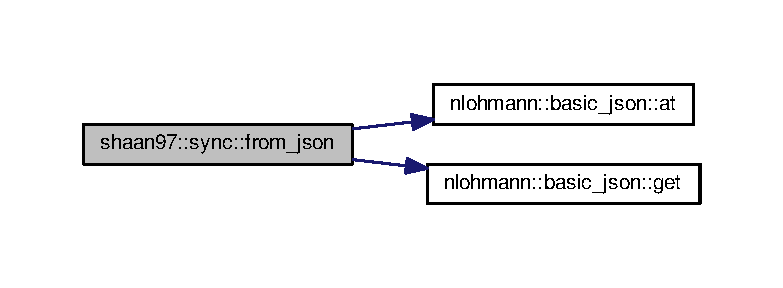
\includegraphics[width=350pt]{group___serialization_gaba06015bb8b13049b093f0bde8e89377_cgraph}
\end{center}
\end{figure}
\mbox{\Hypertarget{group___serialization_ga35dd3deb42a1ec52e00a2980b5c7c842}\label{group___serialization_ga35dd3deb42a1ec52e00a2980b5c7c842}} 
\index{Serialization@{Serialization}!from\+\_\+json@{from\+\_\+json}}
\index{from\+\_\+json@{from\+\_\+json}!Serialization@{Serialization}}
\subsubsection{\texorpdfstring{from\+\_\+json()}{from\_json()}\hspace{0.1cm}{\footnotesize\ttfamily [2/2]}}
{\footnotesize\ttfamily void shaan97\+::sync\+::from\+\_\+json (\begin{DoxyParamCaption}\item[{\hyperlink{namespacenlohmann_a2bfd99e845a2e5cd90aeaf1b1431f474}{nlohmann\+::json} \&}]{j,  }\item[{\hyperlink{classshaan97_1_1sync_1_1_member}{Member} \&}]{m }\end{DoxyParamCaption})}

Converts a {\ttfamily nlohmann\+:json} into a {\ttfamily \hyperlink{classshaan97_1_1sync_1_1_member}{Member}} Here is the call graph for this function\+:
\nopagebreak
\begin{figure}[H]
\begin{center}
\leavevmode
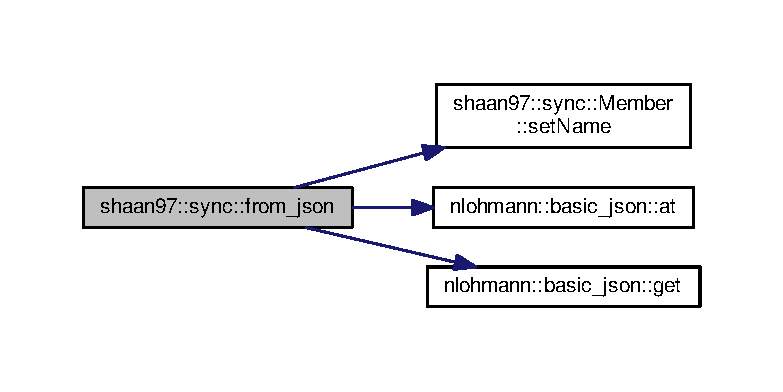
\includegraphics[width=350pt]{group___serialization_ga35dd3deb42a1ec52e00a2980b5c7c842_cgraph}
\end{center}
\end{figure}
\mbox{\Hypertarget{group___serialization_ga213581ca789d5151c699fb4cb30db916}\label{group___serialization_ga213581ca789d5151c699fb4cb30db916}} 
\index{Serialization@{Serialization}!to\+\_\+json@{to\+\_\+json}}
\index{to\+\_\+json@{to\+\_\+json}!Serialization@{Serialization}}
\subsubsection{\texorpdfstring{to\+\_\+json()}{to\_json()}\hspace{0.1cm}{\footnotesize\ttfamily [1/2]}}
{\footnotesize\ttfamily void shaan97\+::sync\+::to\+\_\+json (\begin{DoxyParamCaption}\item[{\hyperlink{namespacenlohmann_a2bfd99e845a2e5cd90aeaf1b1431f474}{nlohmann\+::json} \&}]{j,  }\item[{const \hyperlink{structshaan97_1_1sync_1_1_message}{Message} \&}]{m }\end{DoxyParamCaption})}



Converts a {\ttfamily \hyperlink{structshaan97_1_1sync_1_1_message}{Message}} into a {\ttfamily \hyperlink{namespacenlohmann_a2bfd99e845a2e5cd90aeaf1b1431f474}{nlohmann\+::json} object} 

\mbox{\Hypertarget{group___serialization_gaad90c8bd50725f5382dc2207225f52ee}\label{group___serialization_gaad90c8bd50725f5382dc2207225f52ee}} 
\index{Serialization@{Serialization}!to\+\_\+json@{to\+\_\+json}}
\index{to\+\_\+json@{to\+\_\+json}!Serialization@{Serialization}}
\subsubsection{\texorpdfstring{to\+\_\+json()}{to\_json()}\hspace{0.1cm}{\footnotesize\ttfamily [2/2]}}
{\footnotesize\ttfamily void shaan97\+::sync\+::to\+\_\+json (\begin{DoxyParamCaption}\item[{\hyperlink{namespacenlohmann_a2bfd99e845a2e5cd90aeaf1b1431f474}{nlohmann\+::json} \&}]{j,  }\item[{const \hyperlink{classshaan97_1_1sync_1_1_member}{Member} \&}]{m }\end{DoxyParamCaption})}

Converts a {\ttfamily \hyperlink{classshaan97_1_1sync_1_1_member}{Member}} into a {\ttfamily \hyperlink{namespacenlohmann_a2bfd99e845a2e5cd90aeaf1b1431f474}{nlohmann\+::json}} Here is the call graph for this function\+:\nopagebreak
\begin{figure}[H]
\begin{center}
\leavevmode
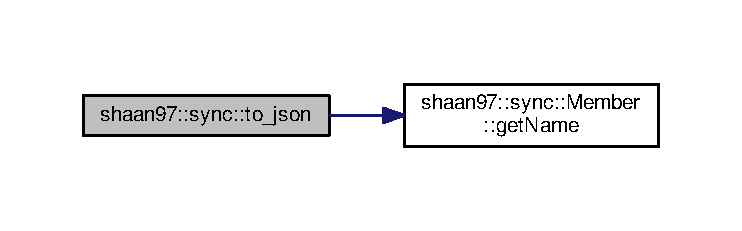
\includegraphics[width=350pt]{group___serialization_gaad90c8bd50725f5382dc2207225f52ee_cgraph}
\end{center}
\end{figure}


\subsection{Friends}
\mbox{\Hypertarget{group___serialization_ga827d73b9e95e7aa59bf1b159251bedf3}\label{group___serialization_ga827d73b9e95e7aa59bf1b159251bedf3}} 
\index{Serialization@{Serialization}!from\+\_\+json@{from\+\_\+json}}
\index{from\+\_\+json@{from\+\_\+json}!Serialization@{Serialization}}
\subsubsection{\texorpdfstring{from\+\_\+json}{from\_json}}
{\footnotesize\ttfamily void from\+\_\+json (\begin{DoxyParamCaption}\item[{\hyperlink{namespacenlohmann_a2bfd99e845a2e5cd90aeaf1b1431f474}{nlohmann\+::json} \&}]{j,  }\item[{\hyperlink{classshaan97_1_1sync_1_1_error}{Error} \&}]{e }\end{DoxyParamCaption})\hspace{0.3cm}{\ttfamily [friend]}}

Converts from {\ttfamily \hyperlink{namespacenlohmann_a2bfd99e845a2e5cd90aeaf1b1431f474}{nlohmann\+::json}} to a {\ttfamily \hyperlink{classshaan97_1_1sync_1_1_error}{Error}} object \mbox{\Hypertarget{group___serialization_ga06e5a619d8d673a3bb00b006e62bbe1e}\label{group___serialization_ga06e5a619d8d673a3bb00b006e62bbe1e}} 
\index{Serialization@{Serialization}!to\+\_\+json@{to\+\_\+json}}
\index{to\+\_\+json@{to\+\_\+json}!Serialization@{Serialization}}
\subsubsection{\texorpdfstring{to\+\_\+json}{to\_json}}
{\footnotesize\ttfamily void to\+\_\+json (\begin{DoxyParamCaption}\item[{\hyperlink{namespacenlohmann_a2bfd99e845a2e5cd90aeaf1b1431f474}{nlohmann\+::json} \&}]{j,  }\item[{const \hyperlink{classshaan97_1_1sync_1_1_error}{Error} \&}]{e }\end{DoxyParamCaption})\hspace{0.3cm}{\ttfamily [friend]}}

Converts from {\ttfamily \hyperlink{classshaan97_1_1sync_1_1_error}{Error}} to a {\ttfamily \hyperlink{namespacenlohmann_a2bfd99e845a2e5cd90aeaf1b1431f474}{nlohmann\+::json}} object 
\hypertarget{group___connection_handling}{}\section{Connection\+Handling}
\label{group___connection_handling}\index{Connection\+Handling@{Connection\+Handling}}
\subsection*{Functions}
\begin{DoxyCompactItemize}
\item 
void \hyperlink{group___connection_handling_gab19cf3e5b775cd1b4eeb6d936340e712}{shaan97\+::sync\+::\+Server\+::start\+\_\+accept} ()
\item 
void \hyperlink{group___connection_handling_ga447569609c9d667ab509e61d1dd1b476}{shaan97\+::sync\+::\+Server\+::handle\+\_\+accept} (std\+::shared\+\_\+ptr$<$ boost\+::asio\+::ip\+::tcp\+::socket $>$ \&socket, const boost\+::system\+::error\+\_\+code \&error)
\end{DoxyCompactItemize}


\subsection{Detailed Description}
Event based system for handling new socket connection.

{\ttfamily \hyperlink{group___connection_handling_gab19cf3e5b775cd1b4eeb6d936340e712}{start\+\_\+accept()}} makes the \hyperlink{classshaan97_1_1sync_1_1_server}{Server} ready for new connections, making {\ttfamily \hyperlink{group___connection_handling_ga447569609c9d667ab509e61d1dd1b476}{handle\+\_\+accept()}} the handler for that asynchronous event. {\ttfamily \hyperlink{group___connection_handling_ga447569609c9d667ab509e61d1dd1b476}{handle\+\_\+accept()}} calls {\ttfamily \hyperlink{group___connection_handling_gab19cf3e5b775cd1b4eeb6d936340e712}{start\+\_\+accept()}} on another thread so that the \hyperlink{classshaan97_1_1sync_1_1_server}{Server} may continue accepting new connections. 

\subsection{Function Documentation}
\mbox{\Hypertarget{group___connection_handling_ga447569609c9d667ab509e61d1dd1b476}\label{group___connection_handling_ga447569609c9d667ab509e61d1dd1b476}} 
\index{Connection\+Handling@{Connection\+Handling}!handle\+\_\+accept@{handle\+\_\+accept}}
\index{handle\+\_\+accept@{handle\+\_\+accept}!Connection\+Handling@{Connection\+Handling}}
\subsubsection{\texorpdfstring{handle\+\_\+accept()}{handle\_accept()}}
{\footnotesize\ttfamily void Server\+::handle\+\_\+accept (\begin{DoxyParamCaption}\item[{std\+::shared\+\_\+ptr$<$ boost\+::asio\+::ip\+::tcp\+::socket $>$ \&}]{socket,  }\item[{const boost\+::system\+::error\+\_\+code \&}]{error }\end{DoxyParamCaption})\hspace{0.3cm}{\ttfamily [private]}}

Handles the connection by reinitiating {\ttfamily \hyperlink{group___connection_handling_gab19cf3e5b775cd1b4eeb6d936340e712}{start\+\_\+accept()}} on another thread and interpreting the message and decides what to do with it. Here is the call graph for this function\+:\nopagebreak
\begin{figure}[H]
\begin{center}
\leavevmode
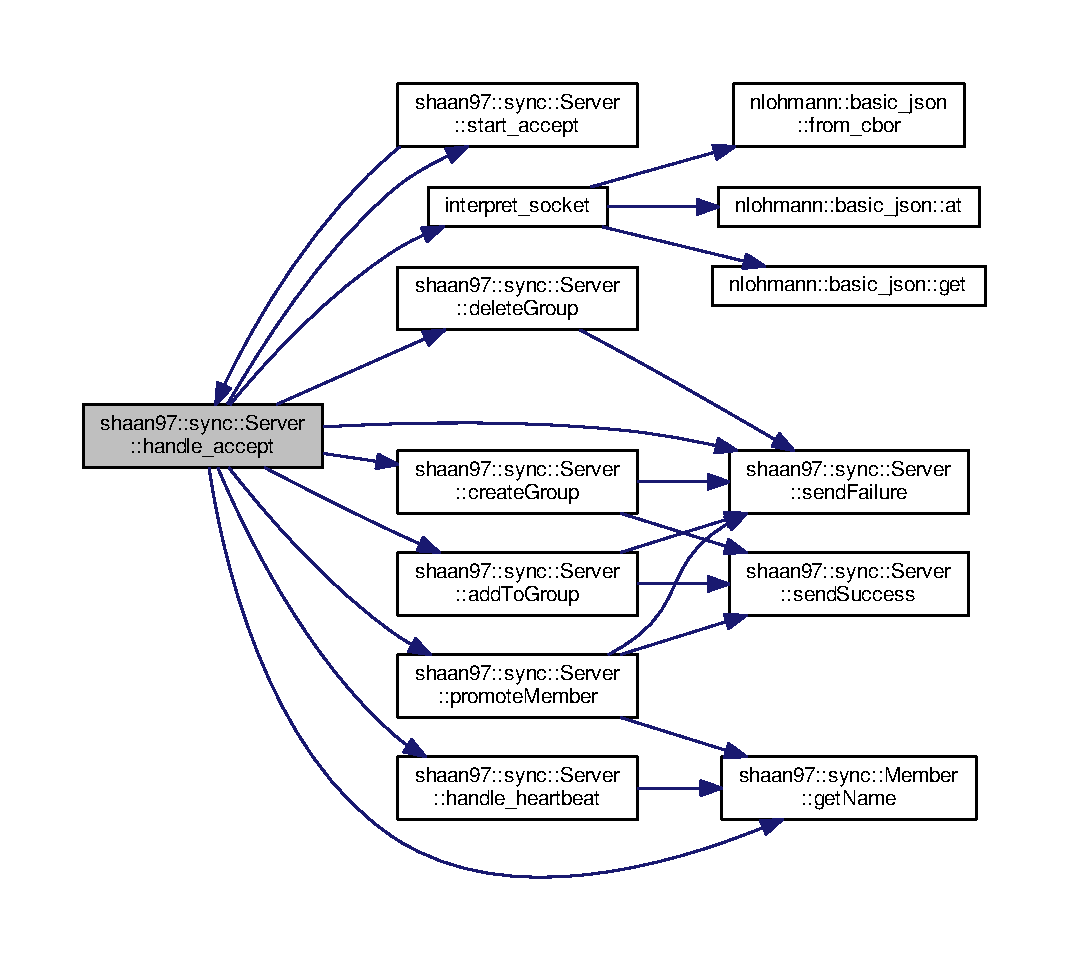
\includegraphics[width=350pt]{group___connection_handling_ga447569609c9d667ab509e61d1dd1b476_cgraph}
\end{center}
\end{figure}
\mbox{\Hypertarget{group___connection_handling_gab19cf3e5b775cd1b4eeb6d936340e712}\label{group___connection_handling_gab19cf3e5b775cd1b4eeb6d936340e712}} 
\index{Connection\+Handling@{Connection\+Handling}!start\+\_\+accept@{start\+\_\+accept}}
\index{start\+\_\+accept@{start\+\_\+accept}!Connection\+Handling@{Connection\+Handling}}
\subsubsection{\texorpdfstring{start\+\_\+accept()}{start\_accept()}}
{\footnotesize\ttfamily void Server\+::start\+\_\+accept (\begin{DoxyParamCaption}{ }\end{DoxyParamCaption})\hspace{0.3cm}{\ttfamily [private]}}

This function prepares the \hyperlink{classshaan97_1_1sync_1_1_server}{Server} for handling new connections. It also sets {\ttfamily handle\+\_\+accept(std\+::shared\+\_\+ptr$<$boost\+::asio\+::ip\+::tcp\+::socket$>$\&, const boost\+::system\+::error\+\_\+code\&)} as the handler for a new connection. Here is the call graph for this function\+:\nopagebreak
\begin{figure}[H]
\begin{center}
\leavevmode
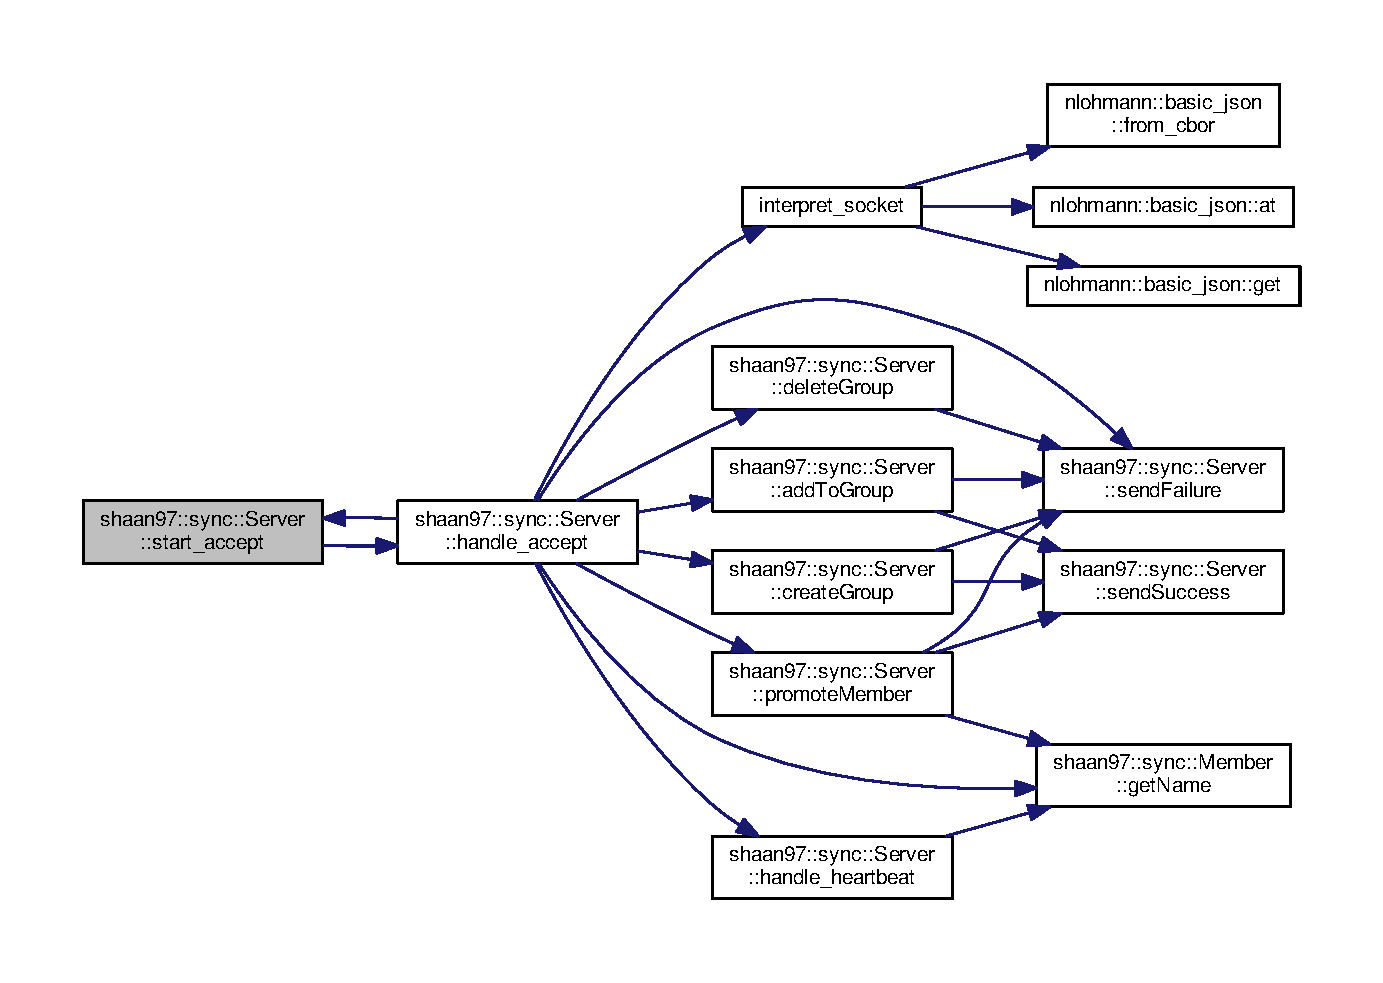
\includegraphics[width=350pt]{group___connection_handling_gab19cf3e5b775cd1b4eeb6d936340e712_cgraph}
\end{center}
\end{figure}

\hypertarget{group___message_handling}{}\section{Message\+Handling}
\label{group___message_handling}\index{Message\+Handling@{Message\+Handling}}
\subsection*{Functions}
\begin{DoxyCompactItemize}
\item 
void \hyperlink{group___message_handling_ga81c419040ae028471a5737c4c0c50e3f}{shaan97\+::sync\+::\+Server\+::create\+Group} (std\+::shared\+\_\+ptr$<$ boost\+::asio\+::ip\+::tcp\+::socket $>$ \&socket, \hyperlink{structshaan97_1_1sync_1_1_message}{Message} \&message)
\item 
void \hyperlink{group___message_handling_gaeb034e1663dff12c80bf7661f6216fe7}{shaan97\+::sync\+::\+Server\+::add\+To\+Group} (std\+::shared\+\_\+ptr$<$ boost\+::asio\+::ip\+::tcp\+::socket $>$ \&socket, \hyperlink{structshaan97_1_1sync_1_1_message}{Message} \&message)
\item 
void \hyperlink{group___message_handling_gaedbdfea1f476a81e5f1ff3b632db9bad}{shaan97\+::sync\+::\+Server\+::delete\+Group} (std\+::shared\+\_\+ptr$<$ boost\+::asio\+::ip\+::tcp\+::socket $>$ \&socket, \hyperlink{structshaan97_1_1sync_1_1_message}{Message} \&message)
\item 
void \hyperlink{group___message_handling_ga56230c5225416d342206232d3f2b8f6e}{shaan97\+::sync\+::\+Server\+::handle\+\_\+heartbeat} (\hyperlink{structshaan97_1_1sync_1_1_message}{Message} \&heartbeat)
\item 
void \hyperlink{group___message_handling_ga46e08d6ffcd45a73aac315e8393e0228}{shaan97\+::sync\+::\+Server\+::promote\+Member} (std\+::shared\+\_\+ptr$<$ boost\+::asio\+::ip\+::tcp\+::socket $>$ \&socket, \hyperlink{structshaan97_1_1sync_1_1_message}{Message} \&message)
\end{DoxyCompactItemize}


\subsection{Detailed Description}
These functions provide the various services that a client can request to the \hyperlink{classshaan97_1_1sync_1_1_server}{Server} These will report success or failure across the socket asynchronously. 

\subsection{Function Documentation}
\mbox{\Hypertarget{group___message_handling_gaeb034e1663dff12c80bf7661f6216fe7}\label{group___message_handling_gaeb034e1663dff12c80bf7661f6216fe7}} 
\index{Message\+Handling@{Message\+Handling}!add\+To\+Group@{add\+To\+Group}}
\index{add\+To\+Group@{add\+To\+Group}!Message\+Handling@{Message\+Handling}}
\subsubsection{\texorpdfstring{add\+To\+Group()}{addToGroup()}}
{\footnotesize\ttfamily void Server\+::add\+To\+Group (\begin{DoxyParamCaption}\item[{std\+::shared\+\_\+ptr$<$ boost\+::asio\+::ip\+::tcp\+::socket $>$ \&}]{socket,  }\item[{\hyperlink{structshaan97_1_1sync_1_1_message}{Message} \&}]{message }\end{DoxyParamCaption})\hspace{0.3cm}{\ttfamily [private]}}

Here is the call graph for this function\+:\nopagebreak
\begin{figure}[H]
\begin{center}
\leavevmode
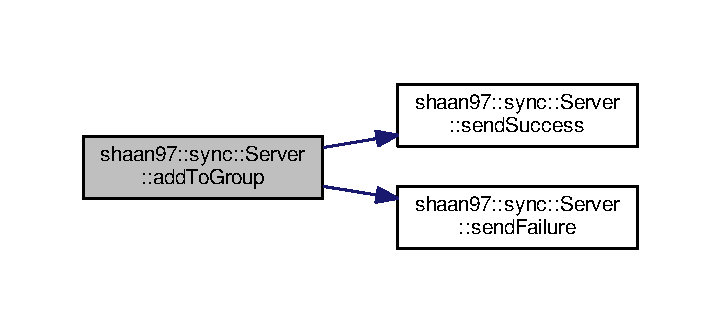
\includegraphics[width=346pt]{group___message_handling_gaeb034e1663dff12c80bf7661f6216fe7_cgraph}
\end{center}
\end{figure}
\mbox{\Hypertarget{group___message_handling_ga81c419040ae028471a5737c4c0c50e3f}\label{group___message_handling_ga81c419040ae028471a5737c4c0c50e3f}} 
\index{Message\+Handling@{Message\+Handling}!create\+Group@{create\+Group}}
\index{create\+Group@{create\+Group}!Message\+Handling@{Message\+Handling}}
\subsubsection{\texorpdfstring{create\+Group()}{createGroup()}}
{\footnotesize\ttfamily void Server\+::create\+Group (\begin{DoxyParamCaption}\item[{std\+::shared\+\_\+ptr$<$ boost\+::asio\+::ip\+::tcp\+::socket $>$ \&}]{socket,  }\item[{\hyperlink{structshaan97_1_1sync_1_1_message}{Message} \&}]{message }\end{DoxyParamCaption})\hspace{0.3cm}{\ttfamily [private]}}

Here is the call graph for this function\+:\nopagebreak
\begin{figure}[H]
\begin{center}
\leavevmode
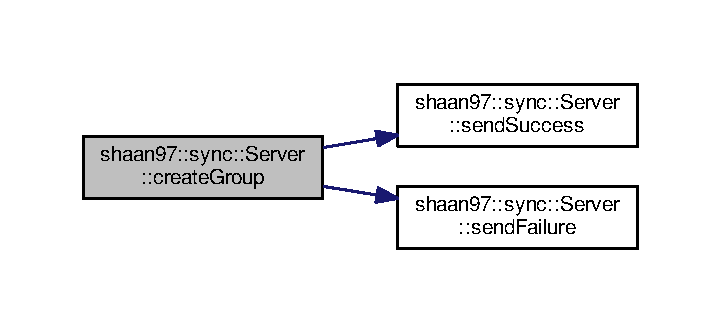
\includegraphics[width=346pt]{group___message_handling_ga81c419040ae028471a5737c4c0c50e3f_cgraph}
\end{center}
\end{figure}
\mbox{\Hypertarget{group___message_handling_gaedbdfea1f476a81e5f1ff3b632db9bad}\label{group___message_handling_gaedbdfea1f476a81e5f1ff3b632db9bad}} 
\index{Message\+Handling@{Message\+Handling}!delete\+Group@{delete\+Group}}
\index{delete\+Group@{delete\+Group}!Message\+Handling@{Message\+Handling}}
\subsubsection{\texorpdfstring{delete\+Group()}{deleteGroup()}}
{\footnotesize\ttfamily void Server\+::delete\+Group (\begin{DoxyParamCaption}\item[{std\+::shared\+\_\+ptr$<$ boost\+::asio\+::ip\+::tcp\+::socket $>$ \&}]{socket,  }\item[{\hyperlink{structshaan97_1_1sync_1_1_message}{Message} \&}]{message }\end{DoxyParamCaption})\hspace{0.3cm}{\ttfamily [private]}}

Here is the call graph for this function\+:\nopagebreak
\begin{figure}[H]
\begin{center}
\leavevmode
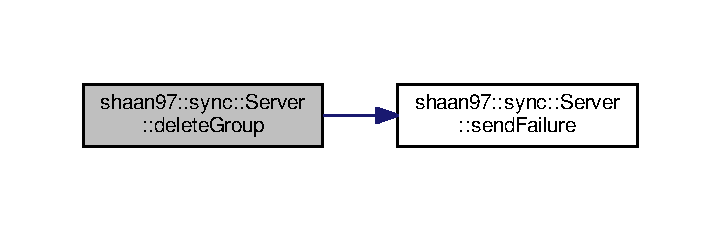
\includegraphics[width=346pt]{group___message_handling_gaedbdfea1f476a81e5f1ff3b632db9bad_cgraph}
\end{center}
\end{figure}
\mbox{\Hypertarget{group___message_handling_ga56230c5225416d342206232d3f2b8f6e}\label{group___message_handling_ga56230c5225416d342206232d3f2b8f6e}} 
\index{Message\+Handling@{Message\+Handling}!handle\+\_\+heartbeat@{handle\+\_\+heartbeat}}
\index{handle\+\_\+heartbeat@{handle\+\_\+heartbeat}!Message\+Handling@{Message\+Handling}}
\subsubsection{\texorpdfstring{handle\+\_\+heartbeat()}{handle\_heartbeat()}}
{\footnotesize\ttfamily void Server\+::handle\+\_\+heartbeat (\begin{DoxyParamCaption}\item[{\hyperlink{structshaan97_1_1sync_1_1_message}{Message} \&}]{heartbeat }\end{DoxyParamCaption})\hspace{0.3cm}{\ttfamily [private]}}

Here is the call graph for this function\+:\nopagebreak
\begin{figure}[H]
\begin{center}
\leavevmode
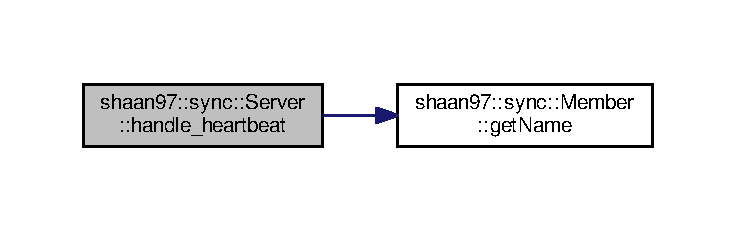
\includegraphics[width=350pt]{group___message_handling_ga56230c5225416d342206232d3f2b8f6e_cgraph}
\end{center}
\end{figure}
\mbox{\Hypertarget{group___message_handling_ga46e08d6ffcd45a73aac315e8393e0228}\label{group___message_handling_ga46e08d6ffcd45a73aac315e8393e0228}} 
\index{Message\+Handling@{Message\+Handling}!promote\+Member@{promote\+Member}}
\index{promote\+Member@{promote\+Member}!Message\+Handling@{Message\+Handling}}
\subsubsection{\texorpdfstring{promote\+Member()}{promoteMember()}}
{\footnotesize\ttfamily void Server\+::promote\+Member (\begin{DoxyParamCaption}\item[{std\+::shared\+\_\+ptr$<$ boost\+::asio\+::ip\+::tcp\+::socket $>$ \&}]{socket,  }\item[{\hyperlink{structshaan97_1_1sync_1_1_message}{Message} \&}]{message }\end{DoxyParamCaption})\hspace{0.3cm}{\ttfamily [private]}}

Here is the call graph for this function\+:\nopagebreak
\begin{figure}[H]
\begin{center}
\leavevmode
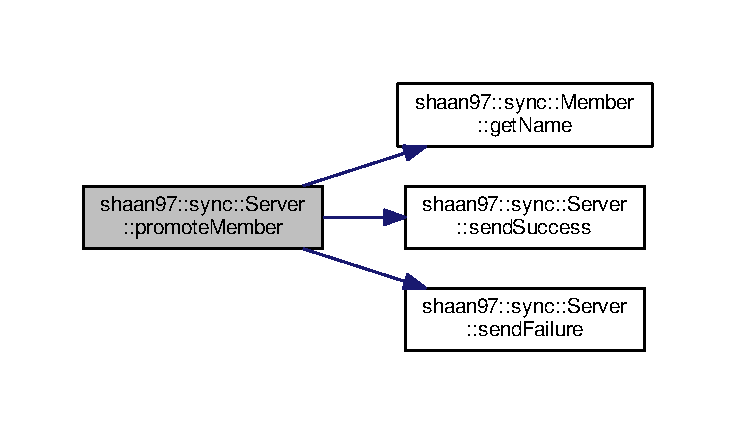
\includegraphics[width=350pt]{group___message_handling_ga46e08d6ffcd45a73aac315e8393e0228_cgraph}
\end{center}
\end{figure}

\hypertarget{group___error_reporting}{}\section{Error\+Reporting}
\label{group___error_reporting}\index{Error\+Reporting@{Error\+Reporting}}
\subsection*{Functions}
\begin{DoxyCompactItemize}
\item 
static void \hyperlink{group___error_reporting_ga360b9e55725804cfba4a86c040001342}{shaan97\+::sync\+::\+Server\+::send\+Failure} (std\+::shared\+\_\+ptr$<$ boost\+::asio\+::ip\+::tcp\+::socket $>$ \&socket, const \hyperlink{classshaan97_1_1sync_1_1_error}{Error} \&error)
\item 
static void \hyperlink{group___error_reporting_gaf606f6afc7f26d76733c7299599dd097}{shaan97\+::sync\+::\+Server\+::send\+Success} (std\+::shared\+\_\+ptr$<$ boost\+::asio\+::ip\+::tcp\+::socket $>$ \&socket)
\item 
static void \hyperlink{group___error_reporting_ga1b81d60d6c76ec6852c73f2749e6e2a4}{shaan97\+::sync\+::\+Server\+::send\+Success} (std\+::shared\+\_\+ptr$<$ boost\+::asio\+::ip\+::tcp\+::socket $>$ \&socket, const \hyperlink{classshaan97_1_1sync_1_1_error}{Error} \&error)
\end{DoxyCompactItemize}


\subsection{Detailed Description}
These functions report success or failure across the socket, (potentially) based upon the value of the {\ttfamily \hyperlink{classshaan97_1_1sync_1_1_error}{shaan97\+::sync\+::\+Error}} object. 

\subsection{Function Documentation}
\mbox{\Hypertarget{group___error_reporting_ga360b9e55725804cfba4a86c040001342}\label{group___error_reporting_ga360b9e55725804cfba4a86c040001342}} 
\index{Error\+Reporting@{Error\+Reporting}!send\+Failure@{send\+Failure}}
\index{send\+Failure@{send\+Failure}!Error\+Reporting@{Error\+Reporting}}
\subsubsection{\texorpdfstring{send\+Failure()}{sendFailure()}}
{\footnotesize\ttfamily void Server\+::send\+Failure (\begin{DoxyParamCaption}\item[{std\+::shared\+\_\+ptr$<$ boost\+::asio\+::ip\+::tcp\+::socket $>$ \&}]{socket,  }\item[{const \hyperlink{classshaan97_1_1sync_1_1_error}{Error} \&}]{error }\end{DoxyParamCaption})\hspace{0.3cm}{\ttfamily [static]}, {\ttfamily [private]}}

\mbox{\Hypertarget{group___error_reporting_gaf606f6afc7f26d76733c7299599dd097}\label{group___error_reporting_gaf606f6afc7f26d76733c7299599dd097}} 
\index{Error\+Reporting@{Error\+Reporting}!send\+Success@{send\+Success}}
\index{send\+Success@{send\+Success}!Error\+Reporting@{Error\+Reporting}}
\subsubsection{\texorpdfstring{send\+Success()}{sendSuccess()}\hspace{0.1cm}{\footnotesize\ttfamily [1/2]}}
{\footnotesize\ttfamily void Server\+::send\+Success (\begin{DoxyParamCaption}\item[{std\+::shared\+\_\+ptr$<$ boost\+::asio\+::ip\+::tcp\+::socket $>$ \&}]{socket }\end{DoxyParamCaption})\hspace{0.3cm}{\ttfamily [static]}, {\ttfamily [private]}}

\mbox{\Hypertarget{group___error_reporting_ga1b81d60d6c76ec6852c73f2749e6e2a4}\label{group___error_reporting_ga1b81d60d6c76ec6852c73f2749e6e2a4}} 
\index{Error\+Reporting@{Error\+Reporting}!send\+Success@{send\+Success}}
\index{send\+Success@{send\+Success}!Error\+Reporting@{Error\+Reporting}}
\subsubsection{\texorpdfstring{send\+Success()}{sendSuccess()}\hspace{0.1cm}{\footnotesize\ttfamily [2/2]}}
{\footnotesize\ttfamily void Server\+::send\+Success (\begin{DoxyParamCaption}\item[{std\+::shared\+\_\+ptr$<$ boost\+::asio\+::ip\+::tcp\+::socket $>$ \&}]{socket,  }\item[{const \hyperlink{classshaan97_1_1sync_1_1_error}{Error} \&}]{error }\end{DoxyParamCaption})\hspace{0.3cm}{\ttfamily [static]}, {\ttfamily [private]}}


\chapter{Namespace Documentation}
\hypertarget{namespacenlohmann}{}\section{nlohmann Namespace Reference}
\label{namespacenlohmann}\index{nlohmann@{nlohmann}}


namespace for Niels Lohmann  


\subsection*{Namespaces}
\begin{DoxyCompactItemize}
\item 
 \hyperlink{namespacenlohmann_1_1detail}{detail}
\begin{DoxyCompactList}\small\item\em unnamed namespace with internal helper functions \end{DoxyCompactList}\end{DoxyCompactItemize}
\subsection*{Classes}
\begin{DoxyCompactItemize}
\item 
struct \hyperlink{structnlohmann_1_1adl__serializer}{adl\+\_\+serializer}
\begin{DoxyCompactList}\small\item\em default J\+S\+O\+N\+Serializer template argument \end{DoxyCompactList}\item 
class \hyperlink{classnlohmann_1_1basic__json}{basic\+\_\+json}
\begin{DoxyCompactList}\small\item\em a class to store J\+S\+ON values \end{DoxyCompactList}\end{DoxyCompactItemize}
\subsection*{Typedefs}
\begin{DoxyCompactItemize}
\item 
using \hyperlink{namespacenlohmann_a2bfd99e845a2e5cd90aeaf1b1431f474}{json} = \hyperlink{classnlohmann_1_1basic__json}{basic\+\_\+json}$<$$>$
\begin{DoxyCompactList}\small\item\em default J\+S\+ON class \end{DoxyCompactList}\end{DoxyCompactItemize}


\subsection{Detailed Description}
namespace for Niels Lohmann 

\begin{DoxySeeAlso}{See also}
\href{https://github.com/nlohmann}{\tt https\+://github.\+com/nlohmann} 
\end{DoxySeeAlso}
\begin{DoxySince}{Since}
version 1.\+0.\+0 
\end{DoxySince}


\subsection{Typedef Documentation}
\mbox{\Hypertarget{namespacenlohmann_a2bfd99e845a2e5cd90aeaf1b1431f474}\label{namespacenlohmann_a2bfd99e845a2e5cd90aeaf1b1431f474}} 
\index{nlohmann@{nlohmann}!json@{json}}
\index{json@{json}!nlohmann@{nlohmann}}
\subsubsection{\texorpdfstring{json}{json}}
{\footnotesize\ttfamily using \hyperlink{namespacenlohmann_a2bfd99e845a2e5cd90aeaf1b1431f474}{nlohmann\+::json} = typedef \hyperlink{classnlohmann_1_1basic__json}{basic\+\_\+json}$<$$>$}



default J\+S\+ON class 

This type is the default specialization of the \hyperlink{classnlohmann_1_1basic__json}{basic\+\_\+json} class which uses the standard template types.

\begin{DoxySince}{Since}
version 1.\+0.\+0 
\end{DoxySince}

\hypertarget{namespacenlohmann_1_1detail}{}\section{nlohmann\+:\+:detail Namespace Reference}
\label{namespacenlohmann_1_1detail}\index{nlohmann\+::detail@{nlohmann\+::detail}}


unnamed namespace with internal helper functions  


\subsection*{Classes}
\begin{DoxyCompactItemize}
\item 
struct \hyperlink{structnlohmann_1_1detail_1_1conjunction}{conjunction}
\item 
struct \hyperlink{structnlohmann_1_1detail_1_1conjunction_3_01_b1_01_4}{conjunction$<$ B1 $>$}
\item 
struct \hyperlink{structnlohmann_1_1detail_1_1conjunction_3_01_b1_00_01_bn_8_8_8_01_4}{conjunction$<$ B1, Bn... $>$}
\item 
struct \hyperlink{structnlohmann_1_1detail_1_1external__constructor}{external\+\_\+constructor}
\item 
struct \hyperlink{structnlohmann_1_1detail_1_1external__constructor_3_01value__t_1_1array_01_4}{external\+\_\+constructor$<$ value\+\_\+t\+::array $>$}
\item 
struct \hyperlink{structnlohmann_1_1detail_1_1external__constructor_3_01value__t_1_1boolean_01_4}{external\+\_\+constructor$<$ value\+\_\+t\+::boolean $>$}
\item 
struct \hyperlink{structnlohmann_1_1detail_1_1external__constructor_3_01value__t_1_1number__float_01_4}{external\+\_\+constructor$<$ value\+\_\+t\+::number\+\_\+float $>$}
\item 
struct \hyperlink{structnlohmann_1_1detail_1_1external__constructor_3_01value__t_1_1number__integer_01_4}{external\+\_\+constructor$<$ value\+\_\+t\+::number\+\_\+integer $>$}
\item 
struct \hyperlink{structnlohmann_1_1detail_1_1external__constructor_3_01value__t_1_1number__unsigned_01_4}{external\+\_\+constructor$<$ value\+\_\+t\+::number\+\_\+unsigned $>$}
\item 
struct \hyperlink{structnlohmann_1_1detail_1_1external__constructor_3_01value__t_1_1object_01_4}{external\+\_\+constructor$<$ value\+\_\+t\+::object $>$}
\item 
struct \hyperlink{structnlohmann_1_1detail_1_1external__constructor_3_01value__t_1_1string_01_4}{external\+\_\+constructor$<$ value\+\_\+t\+::string $>$}
\item 
struct \hyperlink{structnlohmann_1_1detail_1_1from__json__fn}{from\+\_\+json\+\_\+fn}
\item 
struct \hyperlink{structnlohmann_1_1detail_1_1has__from__json}{has\+\_\+from\+\_\+json}
\item 
struct \hyperlink{structnlohmann_1_1detail_1_1has__non__default__from__json}{has\+\_\+non\+\_\+default\+\_\+from\+\_\+json}
\item 
struct \hyperlink{structnlohmann_1_1detail_1_1has__to__json}{has\+\_\+to\+\_\+json}
\item 
struct \hyperlink{structnlohmann_1_1detail_1_1is__basic__json__nested__type}{is\+\_\+basic\+\_\+json\+\_\+nested\+\_\+type}
\item 
struct \hyperlink{structnlohmann_1_1detail_1_1is__compatible__array__type}{is\+\_\+compatible\+\_\+array\+\_\+type}
\item 
struct \hyperlink{structnlohmann_1_1detail_1_1is__compatible__integer__type}{is\+\_\+compatible\+\_\+integer\+\_\+type}
\item 
struct \hyperlink{structnlohmann_1_1detail_1_1is__compatible__integer__type__impl}{is\+\_\+compatible\+\_\+integer\+\_\+type\+\_\+impl}
\item 
struct \hyperlink{structnlohmann_1_1detail_1_1is__compatible__integer__type__impl_3_01true_00_01_real_integer_type78b0ba77f36a8c8169cdb79b01d1a4bf}{is\+\_\+compatible\+\_\+integer\+\_\+type\+\_\+impl$<$ true, Real\+Integer\+Type, Compatible\+Number\+Integer\+Type $>$}
\item 
struct \hyperlink{structnlohmann_1_1detail_1_1is__compatible__object__type}{is\+\_\+compatible\+\_\+object\+\_\+type}
\item 
struct \hyperlink{structnlohmann_1_1detail_1_1is__compatible__object__type__impl}{is\+\_\+compatible\+\_\+object\+\_\+type\+\_\+impl}
\item 
struct \hyperlink{structnlohmann_1_1detail_1_1is__compatible__object__type__impl_3_01true_00_01_real_type_00_01_compatible_object_type_01_4}{is\+\_\+compatible\+\_\+object\+\_\+type\+\_\+impl$<$ true, Real\+Type, Compatible\+Object\+Type $>$}
\item 
struct \hyperlink{structnlohmann_1_1detail_1_1negation}{negation}
\item 
struct \hyperlink{structnlohmann_1_1detail_1_1priority__tag}{priority\+\_\+tag}
\item 
struct \hyperlink{structnlohmann_1_1detail_1_1priority__tag_3_010_01_4}{priority\+\_\+tag$<$ 0 $>$}
\item 
struct \hyperlink{structnlohmann_1_1detail_1_1static__const}{static\+\_\+const}
\item 
struct \hyperlink{structnlohmann_1_1detail_1_1to__json__fn}{to\+\_\+json\+\_\+fn}
\end{DoxyCompactItemize}
\subsection*{Typedefs}
\begin{DoxyCompactItemize}
\item 
{\footnotesize template$<$bool B, typename T  = void$>$ }\\using \hyperlink{namespacenlohmann_1_1detail_a02bcbc878bee413f25b985ada771aa9c}{enable\+\_\+if\+\_\+t} = typename std\+::enable\+\_\+if$<$ B, T $>$\+::type
\item 
{\footnotesize template$<$typename T $>$ }\\using \hyperlink{namespacenlohmann_1_1detail_a53a082eedad9f4729fcd8fed552a21f7}{uncvref\+\_\+t} = typename std\+::remove\+\_\+cv$<$ typename std\+::remove\+\_\+reference$<$ T $>$\+::type $>$\+::type
\item 
{\footnotesize template$<$typename T $>$ }\\using \hyperlink{namespacenlohmann_1_1detail_ab0f6dad10410de436710870e8acc386b}{is\+\_\+unscoped\+\_\+enum} = std\+::integral\+\_\+constant$<$ bool, std\+::is\+\_\+convertible$<$ T, int $>$\+::value and std\+::is\+\_\+enum$<$ T $>$\+::value $>$
\end{DoxyCompactItemize}
\subsection*{Enumerations}
\begin{DoxyCompactItemize}
\item 
enum \hyperlink{namespacenlohmann_1_1detail_a90aa5ef615aa8305e9ea20d8a947980f}{value\+\_\+t} \+: uint8\+\_\+t \{ \newline
\hyperlink{namespacenlohmann_1_1detail_a90aa5ef615aa8305e9ea20d8a947980fa37a6259cc0c1dae299a7866489dff0bd}{value\+\_\+t\+::null}, 
\hyperlink{namespacenlohmann_1_1detail_a90aa5ef615aa8305e9ea20d8a947980faa8cfde6331bd59eb2ac96f8911c4b666}{value\+\_\+t\+::object}, 
\hyperlink{namespacenlohmann_1_1detail_a90aa5ef615aa8305e9ea20d8a947980faf1f713c9e000f5d3f280adbd124df4f5}{value\+\_\+t\+::array}, 
\hyperlink{namespacenlohmann_1_1detail_a90aa5ef615aa8305e9ea20d8a947980fab45cffe084dd3d20d928bee85e7b0f21}{value\+\_\+t\+::string}, 
\newline
\hyperlink{namespacenlohmann_1_1detail_a90aa5ef615aa8305e9ea20d8a947980fa84e2c64f38f78ba3ea5c905ab5a2da27}{value\+\_\+t\+::boolean}, 
\hyperlink{namespacenlohmann_1_1detail_a90aa5ef615aa8305e9ea20d8a947980fa5763da164f8659d94a56e29df64b4bcc}{value\+\_\+t\+::number\+\_\+integer}, 
\hyperlink{namespacenlohmann_1_1detail_a90aa5ef615aa8305e9ea20d8a947980fadce7cc8ec29055c4158828921f2f265e}{value\+\_\+t\+::number\+\_\+unsigned}, 
\hyperlink{namespacenlohmann_1_1detail_a90aa5ef615aa8305e9ea20d8a947980fad9966ecb59667235a57b4b999a649eef}{value\+\_\+t\+::number\+\_\+float}, 
\newline
\hyperlink{namespacenlohmann_1_1detail_a90aa5ef615aa8305e9ea20d8a947980fa94708897ec9db8647dfe695714c98e46}{value\+\_\+t\+::discarded}
 \}\begin{DoxyCompactList}\small\item\em the J\+S\+ON type enumeration \end{DoxyCompactList}
\end{DoxyCompactItemize}
\subsection*{Functions}
\begin{DoxyCompactItemize}
\item 
bool \hyperlink{namespacenlohmann_1_1detail_a09169efff3bd1771fff29bd92cea19e0}{operator$<$} (const \hyperlink{namespacenlohmann_1_1detail_a90aa5ef615aa8305e9ea20d8a947980f}{value\+\_\+t} lhs, const \hyperlink{namespacenlohmann_1_1detail_a90aa5ef615aa8305e9ea20d8a947980f}{value\+\_\+t} rhs) noexcept
\begin{DoxyCompactList}\small\item\em comparison operator for J\+S\+ON types \end{DoxyCompactList}\item 
\hyperlink{namespacenlohmann_1_1detail_a7b2601c238073c43a07862768b319cf8}{N\+L\+O\+H\+M\+A\+N\+N\+\_\+\+J\+S\+O\+N\+\_\+\+H\+A\+S\+\_\+\+H\+E\+L\+P\+ER} (mapped\+\_\+type)
\item 
\hyperlink{namespacenlohmann_1_1detail_ad19328f0c4ffe2890ecafb7c89e0355b}{N\+L\+O\+H\+M\+A\+N\+N\+\_\+\+J\+S\+O\+N\+\_\+\+H\+A\+S\+\_\+\+H\+E\+L\+P\+ER} (key\+\_\+type)
\item 
\hyperlink{namespacenlohmann_1_1detail_af3e900eb1e0b107c812f7babbb94e69e}{N\+L\+O\+H\+M\+A\+N\+N\+\_\+\+J\+S\+O\+N\+\_\+\+H\+A\+S\+\_\+\+H\+E\+L\+P\+ER} (value\+\_\+type)
\item 
\hyperlink{namespacenlohmann_1_1detail_a6648328c4b1466fdc48f1fcfbff23e2f}{N\+L\+O\+H\+M\+A\+N\+N\+\_\+\+J\+S\+O\+N\+\_\+\+H\+A\+S\+\_\+\+H\+E\+L\+P\+ER} (iterator)
\item 
{\footnotesize template$<$typename Basic\+Json\+Type , typename T , enable\+\_\+if\+\_\+t$<$ std\+::is\+\_\+same$<$ T, typename Basic\+Json\+Type\+::boolean\+\_\+t $>$\+::value, int $>$  = 0$>$ }\\void \hyperlink{namespacenlohmann_1_1detail_a1a804b98cbe89b7e44b698f2ca860490}{to\+\_\+json} (Basic\+Json\+Type \&j, T b) noexcept
\item 
{\footnotesize template$<$typename Basic\+Json\+Type , typename Compatible\+String , enable\+\_\+if\+\_\+t$<$ std\+::is\+\_\+constructible$<$ typename Basic\+Json\+Type\+::string\+\_\+t, Compatible\+String $>$\+::value, int $>$  = 0$>$ }\\void \hyperlink{namespacenlohmann_1_1detail_a7356ed05cdbbb080cee80e1211e1c6c9}{to\+\_\+json} (Basic\+Json\+Type \&j, const Compatible\+String \&s)
\item 
{\footnotesize template$<$typename Basic\+Json\+Type , typename Float\+Type , enable\+\_\+if\+\_\+t$<$ std\+::is\+\_\+floating\+\_\+point$<$ Float\+Type $>$\+::value, int $>$  = 0$>$ }\\void \hyperlink{namespacenlohmann_1_1detail_a22bffdc8bc7e43af380ba2050696b230}{to\+\_\+json} (Basic\+Json\+Type \&j, Float\+Type val) noexcept
\item 
{\footnotesize template$<$typename Basic\+Json\+Type , typename Compatible\+Number\+Unsigned\+Type , enable\+\_\+if\+\_\+t$<$ is\+\_\+compatible\+\_\+integer\+\_\+type$<$ typename Basic\+Json\+Type\+::number\+\_\+unsigned\+\_\+t, Compatible\+Number\+Unsigned\+Type $>$\+::value, int $>$  = 0$>$ }\\void \hyperlink{namespacenlohmann_1_1detail_ae5fd66b5517b3b5a6c6b9fd9f29ba8dc}{to\+\_\+json} (Basic\+Json\+Type \&j, Compatible\+Number\+Unsigned\+Type val) noexcept
\item 
{\footnotesize template$<$typename Basic\+Json\+Type , typename Compatible\+Number\+Integer\+Type , enable\+\_\+if\+\_\+t$<$ is\+\_\+compatible\+\_\+integer\+\_\+type$<$ typename Basic\+Json\+Type\+::number\+\_\+integer\+\_\+t, Compatible\+Number\+Integer\+Type $>$\+::value, int $>$  = 0$>$ }\\void \hyperlink{namespacenlohmann_1_1detail_a91fe576be579c8c2fdd14610605c6dd2}{to\+\_\+json} (Basic\+Json\+Type \&j, Compatible\+Number\+Integer\+Type val) noexcept
\item 
{\footnotesize template$<$typename Basic\+Json\+Type , typename Unscoped\+Enum\+Type , enable\+\_\+if\+\_\+t$<$ is\+\_\+unscoped\+\_\+enum$<$ Unscoped\+Enum\+Type $>$\+::value, int $>$  = 0$>$ }\\void \hyperlink{namespacenlohmann_1_1detail_a1f83504de38ee6f440a77ae898b86a18}{to\+\_\+json} (Basic\+Json\+Type \&j, Unscoped\+Enum\+Type e) noexcept
\item 
{\footnotesize template$<$typename Basic\+Json\+Type , typename Compatible\+Array\+Type , enable\+\_\+if\+\_\+t$<$ is\+\_\+compatible\+\_\+array\+\_\+type$<$ Basic\+Json\+Type, Compatible\+Array\+Type $>$\+::value or std\+::is\+\_\+same$<$ typename Basic\+Json\+Type\+::array\+\_\+t, Compatible\+Array\+Type $>$\+::value, int $>$  = 0$>$ }\\void \hyperlink{namespacenlohmann_1_1detail_a3afebc132c5ff83f9cd160e52030fdfd}{to\+\_\+json} (Basic\+Json\+Type \&j, const Compatible\+Array\+Type \&arr)
\item 
{\footnotesize template$<$typename Basic\+Json\+Type , typename Compatible\+Object\+Type , enable\+\_\+if\+\_\+t$<$ is\+\_\+compatible\+\_\+object\+\_\+type$<$ Basic\+Json\+Type, Compatible\+Object\+Type $>$\+::value, int $>$  = 0$>$ }\\void \hyperlink{namespacenlohmann_1_1detail_a6fa2f784014bfc0b62d7a35d51e676c9}{to\+\_\+json} (Basic\+Json\+Type \&j, const Compatible\+Object\+Type \&arr)
\item 
{\footnotesize template$<$typename Basic\+Json\+Type , typename Arithmetic\+Type , enable\+\_\+if\+\_\+t$<$ std\+::is\+\_\+arithmetic$<$ Arithmetic\+Type $>$\+::value and not std\+::is\+\_\+same$<$ Arithmetic\+Type, typename Basic\+Json\+Type\+::boolean\+\_\+t $>$\+::value, int $>$  = 0$>$ }\\void \hyperlink{namespacenlohmann_1_1detail_a85955b9c6dd31846e4b8e891f78614b6}{get\+\_\+arithmetic\+\_\+value} (const Basic\+Json\+Type \&j, Arithmetic\+Type \&val)
\item 
{\footnotesize template$<$typename Basic\+Json\+Type $>$ }\\void \hyperlink{namespacenlohmann_1_1detail_a58117f225f43d03e3a0a4a6f3d77c9d9}{from\+\_\+json} (const Basic\+Json\+Type \&j, typename Basic\+Json\+Type\+::boolean\+\_\+t \&b)
\item 
{\footnotesize template$<$typename Basic\+Json\+Type $>$ }\\void \hyperlink{namespacenlohmann_1_1detail_ad74d89f77ada7a57eff38b43d4bf2335}{from\+\_\+json} (const Basic\+Json\+Type \&j, typename Basic\+Json\+Type\+::string\+\_\+t \&s)
\item 
{\footnotesize template$<$typename Basic\+Json\+Type $>$ }\\void \hyperlink{namespacenlohmann_1_1detail_a7cb5dd7d46a60e65f9a8e0873b3f7dd8}{from\+\_\+json} (const Basic\+Json\+Type \&j, typename Basic\+Json\+Type\+::number\+\_\+float\+\_\+t \&val)
\item 
{\footnotesize template$<$typename Basic\+Json\+Type $>$ }\\void \hyperlink{namespacenlohmann_1_1detail_ace4d5680ba413d9fd897ccb5d9c61a1c}{from\+\_\+json} (const Basic\+Json\+Type \&j, typename Basic\+Json\+Type\+::number\+\_\+unsigned\+\_\+t \&val)
\item 
{\footnotesize template$<$typename Basic\+Json\+Type $>$ }\\void \hyperlink{namespacenlohmann_1_1detail_a047d881e611fcac709dc318f730a1732}{from\+\_\+json} (const Basic\+Json\+Type \&j, typename Basic\+Json\+Type\+::number\+\_\+integer\+\_\+t \&val)
\item 
{\footnotesize template$<$typename Basic\+Json\+Type , typename Unscoped\+Enum\+Type , enable\+\_\+if\+\_\+t$<$ is\+\_\+unscoped\+\_\+enum$<$ Unscoped\+Enum\+Type $>$\+::value, int $>$  = 0$>$ }\\void \hyperlink{namespacenlohmann_1_1detail_acf8dd944c2c7455880dee6f0b355aa01}{from\+\_\+json} (const Basic\+Json\+Type \&j, Unscoped\+Enum\+Type \&e)
\item 
{\footnotesize template$<$typename Basic\+Json\+Type $>$ }\\void \hyperlink{namespacenlohmann_1_1detail_abc62958462b916726b89f25fa381a129}{from\+\_\+json} (const Basic\+Json\+Type \&j, typename Basic\+Json\+Type\+::array\+\_\+t \&arr)
\item 
{\footnotesize template$<$typename Basic\+Json\+Type , typename T , typename Allocator $>$ }\\void \hyperlink{namespacenlohmann_1_1detail_a7fb5b5b8034d347b702d31d7fec4ecd7}{from\+\_\+json} (const Basic\+Json\+Type \&j, std\+::forward\+\_\+list$<$ T, Allocator $>$ \&l)
\item 
{\footnotesize template$<$typename Basic\+Json\+Type , typename Compatible\+Array\+Type $>$ }\\void \hyperlink{namespacenlohmann_1_1detail_ac53673a5ce29fb69b96d41dad33cb3b0}{from\+\_\+json\+\_\+array\+\_\+impl} (const Basic\+Json\+Type \&j, Compatible\+Array\+Type \&arr, \hyperlink{structnlohmann_1_1detail_1_1priority__tag}{priority\+\_\+tag}$<$ 0 $>$)
\item 
{\footnotesize template$<$typename Basic\+Json\+Type , typename Compatible\+Array\+Type $>$ }\\auto \hyperlink{namespacenlohmann_1_1detail_a57f93ed57254a1639087cdc316e0fb83}{from\+\_\+json\+\_\+array\+\_\+impl} (const Basic\+Json\+Type \&j, Compatible\+Array\+Type \&arr, \hyperlink{structnlohmann_1_1detail_1_1priority__tag}{priority\+\_\+tag}$<$ 1 $>$) -\/$>$ decltype(arr.\+reserve(std\+::declval$<$ typename Compatible\+Array\+Type\+::size\+\_\+type $>$()), void())
\item 
{\footnotesize template$<$typename Basic\+Json\+Type , typename Compatible\+Array\+Type , enable\+\_\+if\+\_\+t$<$ is\+\_\+compatible\+\_\+array\+\_\+type$<$ Basic\+Json\+Type, Compatible\+Array\+Type $>$\+::value and not std\+::is\+\_\+same$<$ typename Basic\+Json\+Type\+::array\+\_\+t, Compatible\+Array\+Type $>$\+::value, int $>$  = 0$>$ }\\void \hyperlink{namespacenlohmann_1_1detail_a8dcac00852dbe1f61d1e78135b19d428}{from\+\_\+json} (const Basic\+Json\+Type \&j, Compatible\+Array\+Type \&arr)
\item 
{\footnotesize template$<$typename Basic\+Json\+Type , typename Compatible\+Object\+Type , enable\+\_\+if\+\_\+t$<$ is\+\_\+compatible\+\_\+object\+\_\+type$<$ Basic\+Json\+Type, Compatible\+Object\+Type $>$\+::value, int $>$  = 0$>$ }\\void \hyperlink{namespacenlohmann_1_1detail_a5e7a3674e8ac46f8feebad9712d7c55f}{from\+\_\+json} (const Basic\+Json\+Type \&j, Compatible\+Object\+Type \&obj)
\item 
{\footnotesize template$<$typename Basic\+Json\+Type , typename Arithmetic\+Type , enable\+\_\+if\+\_\+t$<$ std\+::is\+\_\+arithmetic$<$ Arithmetic\+Type $>$\+::value and not std\+::is\+\_\+same$<$ Arithmetic\+Type, typename Basic\+Json\+Type\+::number\+\_\+unsigned\+\_\+t $>$\+::value and not std\+::is\+\_\+same$<$ Arithmetic\+Type, typename Basic\+Json\+Type\+::number\+\_\+integer\+\_\+t $>$\+::value and not std\+::is\+\_\+same$<$ Arithmetic\+Type, typename Basic\+Json\+Type\+::number\+\_\+float\+\_\+t $>$\+::value and not std\+::is\+\_\+same$<$ Arithmetic\+Type, typename Basic\+Json\+Type\+::boolean\+\_\+t $>$\+::value, int $>$  = 0$>$ }\\void \hyperlink{namespacenlohmann_1_1detail_a839b0ab50d2c9bce669068f56bc41202}{from\+\_\+json} (const Basic\+Json\+Type \&j, Arithmetic\+Type \&val)
\end{DoxyCompactItemize}


\subsection{Detailed Description}
unnamed namespace with internal helper functions 

This namespace collects some functions that could not be defined inside the \hyperlink{classnlohmann_1_1basic__json}{basic\+\_\+json} class.

\begin{DoxySince}{Since}
version 2.\+1.\+0 
\end{DoxySince}


\subsection{Typedef Documentation}
\mbox{\Hypertarget{namespacenlohmann_1_1detail_a02bcbc878bee413f25b985ada771aa9c}\label{namespacenlohmann_1_1detail_a02bcbc878bee413f25b985ada771aa9c}} 
\index{nlohmann\+::detail@{nlohmann\+::detail}!enable\+\_\+if\+\_\+t@{enable\+\_\+if\+\_\+t}}
\index{enable\+\_\+if\+\_\+t@{enable\+\_\+if\+\_\+t}!nlohmann\+::detail@{nlohmann\+::detail}}
\subsubsection{\texorpdfstring{enable\+\_\+if\+\_\+t}{enable\_if\_t}}
{\footnotesize\ttfamily template$<$bool B, typename T  = void$>$ \\
using \hyperlink{namespacenlohmann_1_1detail_a02bcbc878bee413f25b985ada771aa9c}{nlohmann\+::detail\+::enable\+\_\+if\+\_\+t} = typedef typename std\+::enable\+\_\+if$<$B, T$>$\+::type}

\mbox{\Hypertarget{namespacenlohmann_1_1detail_ab0f6dad10410de436710870e8acc386b}\label{namespacenlohmann_1_1detail_ab0f6dad10410de436710870e8acc386b}} 
\index{nlohmann\+::detail@{nlohmann\+::detail}!is\+\_\+unscoped\+\_\+enum@{is\+\_\+unscoped\+\_\+enum}}
\index{is\+\_\+unscoped\+\_\+enum@{is\+\_\+unscoped\+\_\+enum}!nlohmann\+::detail@{nlohmann\+::detail}}
\subsubsection{\texorpdfstring{is\+\_\+unscoped\+\_\+enum}{is\_unscoped\_enum}}
{\footnotesize\ttfamily template$<$typename T $>$ \\
using \hyperlink{namespacenlohmann_1_1detail_ab0f6dad10410de436710870e8acc386b}{nlohmann\+::detail\+::is\+\_\+unscoped\+\_\+enum} = typedef std\+::integral\+\_\+constant$<$bool, std\+::is\+\_\+convertible$<$T, int$>$\+::value and std\+::is\+\_\+enum$<$T$>$\+::value$>$}

\mbox{\Hypertarget{namespacenlohmann_1_1detail_a53a082eedad9f4729fcd8fed552a21f7}\label{namespacenlohmann_1_1detail_a53a082eedad9f4729fcd8fed552a21f7}} 
\index{nlohmann\+::detail@{nlohmann\+::detail}!uncvref\+\_\+t@{uncvref\+\_\+t}}
\index{uncvref\+\_\+t@{uncvref\+\_\+t}!nlohmann\+::detail@{nlohmann\+::detail}}
\subsubsection{\texorpdfstring{uncvref\+\_\+t}{uncvref\_t}}
{\footnotesize\ttfamily template$<$typename T $>$ \\
using \hyperlink{namespacenlohmann_1_1detail_a53a082eedad9f4729fcd8fed552a21f7}{nlohmann\+::detail\+::uncvref\+\_\+t} = typedef typename std\+::remove\+\_\+cv$<$typename std\+::remove\+\_\+reference$<$T$>$\+::type$>$\+::type}



\subsection{Enumeration Type Documentation}
\mbox{\Hypertarget{namespacenlohmann_1_1detail_a90aa5ef615aa8305e9ea20d8a947980f}\label{namespacenlohmann_1_1detail_a90aa5ef615aa8305e9ea20d8a947980f}} 
\index{nlohmann\+::detail@{nlohmann\+::detail}!value\+\_\+t@{value\+\_\+t}}
\index{value\+\_\+t@{value\+\_\+t}!nlohmann\+::detail@{nlohmann\+::detail}}
\subsubsection{\texorpdfstring{value\+\_\+t}{value\_t}}
{\footnotesize\ttfamily enum \hyperlink{namespacenlohmann_1_1detail_a90aa5ef615aa8305e9ea20d8a947980f}{nlohmann\+::detail\+::value\+\_\+t} \+: uint8\+\_\+t\hspace{0.3cm}{\ttfamily [strong]}}



the J\+S\+ON type enumeration 

This enumeration collects the different J\+S\+ON types. It is internally used to distinguish the stored values, and the functions \hyperlink{classnlohmann_1_1basic__json_a8faa039ca82427ed29c486ffd00600c3}{basic\+\_\+json\+::is\+\_\+null()}, \hyperlink{classnlohmann_1_1basic__json_af8f511af124e82e4579f444b4175787c}{basic\+\_\+json\+::is\+\_\+object()}, \hyperlink{classnlohmann_1_1basic__json_aef9ce5dd2381caee1f8ddcdb5bdd9c65}{basic\+\_\+json\+::is\+\_\+array()}, \hyperlink{classnlohmann_1_1basic__json_a69b596a4a6683b362095c9a139637396}{basic\+\_\+json\+::is\+\_\+string()}, \hyperlink{classnlohmann_1_1basic__json_a943e8cb182d0f2365c76d64b42eaa6fd}{basic\+\_\+json\+::is\+\_\+boolean()}, \hyperlink{classnlohmann_1_1basic__json_a2b9852390abb4b1ef5fac6984e2fc0f3}{basic\+\_\+json\+::is\+\_\+number()} (with \hyperlink{classnlohmann_1_1basic__json_abac8af76067f1e8fdca9052882c74428}{basic\+\_\+json\+::is\+\_\+number\+\_\+integer()}, \hyperlink{classnlohmann_1_1basic__json_abc7378cba0613a78b9aad1c8e7044bb0}{basic\+\_\+json\+::is\+\_\+number\+\_\+unsigned()}, and \hyperlink{classnlohmann_1_1basic__json_a33b4bf898b857c962e798fc7f6e86e70}{basic\+\_\+json\+::is\+\_\+number\+\_\+float()}), \hyperlink{classnlohmann_1_1basic__json_aabe623bc8304c2ba92d96d91f390fab4}{basic\+\_\+json\+::is\+\_\+discarded()}, \hyperlink{classnlohmann_1_1basic__json_a6362b88718eb5c6d4fed6a61eed44b95}{basic\+\_\+json\+::is\+\_\+primitive()}, and \hyperlink{classnlohmann_1_1basic__json_a9f68a0af820c3ced7f9d17851ce4c22d}{basic\+\_\+json\+::is\+\_\+structured()} rely on it.

\begin{DoxyNote}{Note}
There are three enumeration entries (number\+\_\+integer, number\+\_\+unsigned, and number\+\_\+float), because the library distinguishes these three types for numbers\+: \hyperlink{classnlohmann_1_1basic__json_ab906e29b5d83ac162e823ada2156b989}{basic\+\_\+json\+::number\+\_\+unsigned\+\_\+t} is used for unsigned integers, \hyperlink{classnlohmann_1_1basic__json_a98e611d67b7bd75307de99c9358ab2dc}{basic\+\_\+json\+::number\+\_\+integer\+\_\+t} is used for signed integers, and \hyperlink{classnlohmann_1_1basic__json_a88d6103cb3620410b35200ee8e313d97}{basic\+\_\+json\+::number\+\_\+float\+\_\+t} is used for floating-\/point numbers or to approximate integers which do not fit in the limits of their respective type.
\end{DoxyNote}
\begin{DoxySeeAlso}{See also}
\hyperlink{classnlohmann_1_1basic__json_a32124a16dc80729d964d9caf607c2bc8}{basic\+\_\+json\+::basic\+\_\+json(const value\+\_\+t value\+\_\+type)} -- create a J\+S\+ON value with the default value for a given type
\end{DoxySeeAlso}
\begin{DoxySince}{Since}
version 1.\+0.\+0 
\end{DoxySince}
\begin{DoxyEnumFields}{Enumerator}
\raisebox{\heightof{T}}[0pt][0pt]{\index{null@{null}!nlohmann\+::detail@{nlohmann\+::detail}}\index{nlohmann\+::detail@{nlohmann\+::detail}!null@{null}}}\mbox{\Hypertarget{namespacenlohmann_1_1detail_a90aa5ef615aa8305e9ea20d8a947980fa37a6259cc0c1dae299a7866489dff0bd}\label{namespacenlohmann_1_1detail_a90aa5ef615aa8305e9ea20d8a947980fa37a6259cc0c1dae299a7866489dff0bd}} 
null&null value \\
\hline

\raisebox{\heightof{T}}[0pt][0pt]{\index{object@{object}!nlohmann\+::detail@{nlohmann\+::detail}}\index{nlohmann\+::detail@{nlohmann\+::detail}!object@{object}}}\mbox{\Hypertarget{namespacenlohmann_1_1detail_a90aa5ef615aa8305e9ea20d8a947980faa8cfde6331bd59eb2ac96f8911c4b666}\label{namespacenlohmann_1_1detail_a90aa5ef615aa8305e9ea20d8a947980faa8cfde6331bd59eb2ac96f8911c4b666}} 
object&object (unordered set of name/value pairs) \\
\hline

\raisebox{\heightof{T}}[0pt][0pt]{\index{array@{array}!nlohmann\+::detail@{nlohmann\+::detail}}\index{nlohmann\+::detail@{nlohmann\+::detail}!array@{array}}}\mbox{\Hypertarget{namespacenlohmann_1_1detail_a90aa5ef615aa8305e9ea20d8a947980faf1f713c9e000f5d3f280adbd124df4f5}\label{namespacenlohmann_1_1detail_a90aa5ef615aa8305e9ea20d8a947980faf1f713c9e000f5d3f280adbd124df4f5}} 
array&array (ordered collection of values) \\
\hline

\raisebox{\heightof{T}}[0pt][0pt]{\index{string@{string}!nlohmann\+::detail@{nlohmann\+::detail}}\index{nlohmann\+::detail@{nlohmann\+::detail}!string@{string}}}\mbox{\Hypertarget{namespacenlohmann_1_1detail_a90aa5ef615aa8305e9ea20d8a947980fab45cffe084dd3d20d928bee85e7b0f21}\label{namespacenlohmann_1_1detail_a90aa5ef615aa8305e9ea20d8a947980fab45cffe084dd3d20d928bee85e7b0f21}} 
string&string value \\
\hline

\raisebox{\heightof{T}}[0pt][0pt]{\index{boolean@{boolean}!nlohmann\+::detail@{nlohmann\+::detail}}\index{nlohmann\+::detail@{nlohmann\+::detail}!boolean@{boolean}}}\mbox{\Hypertarget{namespacenlohmann_1_1detail_a90aa5ef615aa8305e9ea20d8a947980fa84e2c64f38f78ba3ea5c905ab5a2da27}\label{namespacenlohmann_1_1detail_a90aa5ef615aa8305e9ea20d8a947980fa84e2c64f38f78ba3ea5c905ab5a2da27}} 
boolean&boolean value \\
\hline

\raisebox{\heightof{T}}[0pt][0pt]{\index{number\+\_\+integer@{number\+\_\+integer}!nlohmann\+::detail@{nlohmann\+::detail}}\index{nlohmann\+::detail@{nlohmann\+::detail}!number\+\_\+integer@{number\+\_\+integer}}}\mbox{\Hypertarget{namespacenlohmann_1_1detail_a90aa5ef615aa8305e9ea20d8a947980fa5763da164f8659d94a56e29df64b4bcc}\label{namespacenlohmann_1_1detail_a90aa5ef615aa8305e9ea20d8a947980fa5763da164f8659d94a56e29df64b4bcc}} 
number\+\_\+integer&number value (signed integer) \\
\hline

\raisebox{\heightof{T}}[0pt][0pt]{\index{number\+\_\+unsigned@{number\+\_\+unsigned}!nlohmann\+::detail@{nlohmann\+::detail}}\index{nlohmann\+::detail@{nlohmann\+::detail}!number\+\_\+unsigned@{number\+\_\+unsigned}}}\mbox{\Hypertarget{namespacenlohmann_1_1detail_a90aa5ef615aa8305e9ea20d8a947980fadce7cc8ec29055c4158828921f2f265e}\label{namespacenlohmann_1_1detail_a90aa5ef615aa8305e9ea20d8a947980fadce7cc8ec29055c4158828921f2f265e}} 
number\+\_\+unsigned&number value (unsigned integer) \\
\hline

\raisebox{\heightof{T}}[0pt][0pt]{\index{number\+\_\+float@{number\+\_\+float}!nlohmann\+::detail@{nlohmann\+::detail}}\index{nlohmann\+::detail@{nlohmann\+::detail}!number\+\_\+float@{number\+\_\+float}}}\mbox{\Hypertarget{namespacenlohmann_1_1detail_a90aa5ef615aa8305e9ea20d8a947980fad9966ecb59667235a57b4b999a649eef}\label{namespacenlohmann_1_1detail_a90aa5ef615aa8305e9ea20d8a947980fad9966ecb59667235a57b4b999a649eef}} 
number\+\_\+float&number value (floating-\/point) \\
\hline

\raisebox{\heightof{T}}[0pt][0pt]{\index{discarded@{discarded}!nlohmann\+::detail@{nlohmann\+::detail}}\index{nlohmann\+::detail@{nlohmann\+::detail}!discarded@{discarded}}}\mbox{\Hypertarget{namespacenlohmann_1_1detail_a90aa5ef615aa8305e9ea20d8a947980fa94708897ec9db8647dfe695714c98e46}\label{namespacenlohmann_1_1detail_a90aa5ef615aa8305e9ea20d8a947980fa94708897ec9db8647dfe695714c98e46}} 
discarded&discarded by the the parser callback function \\
\hline

\end{DoxyEnumFields}


\subsection{Function Documentation}
\mbox{\Hypertarget{namespacenlohmann_1_1detail_a58117f225f43d03e3a0a4a6f3d77c9d9}\label{namespacenlohmann_1_1detail_a58117f225f43d03e3a0a4a6f3d77c9d9}} 
\index{nlohmann\+::detail@{nlohmann\+::detail}!from\+\_\+json@{from\+\_\+json}}
\index{from\+\_\+json@{from\+\_\+json}!nlohmann\+::detail@{nlohmann\+::detail}}
\subsubsection{\texorpdfstring{from\+\_\+json()}{from\_json()}\hspace{0.1cm}{\footnotesize\ttfamily [1/11]}}
{\footnotesize\ttfamily template$<$typename Basic\+Json\+Type $>$ \\
void nlohmann\+::detail\+::from\+\_\+json (\begin{DoxyParamCaption}\item[{const Basic\+Json\+Type \&}]{j,  }\item[{typename Basic\+Json\+Type\+::boolean\+\_\+t \&}]{b }\end{DoxyParamCaption})}

\mbox{\Hypertarget{namespacenlohmann_1_1detail_ad74d89f77ada7a57eff38b43d4bf2335}\label{namespacenlohmann_1_1detail_ad74d89f77ada7a57eff38b43d4bf2335}} 
\index{nlohmann\+::detail@{nlohmann\+::detail}!from\+\_\+json@{from\+\_\+json}}
\index{from\+\_\+json@{from\+\_\+json}!nlohmann\+::detail@{nlohmann\+::detail}}
\subsubsection{\texorpdfstring{from\+\_\+json()}{from\_json()}\hspace{0.1cm}{\footnotesize\ttfamily [2/11]}}
{\footnotesize\ttfamily template$<$typename Basic\+Json\+Type $>$ \\
void nlohmann\+::detail\+::from\+\_\+json (\begin{DoxyParamCaption}\item[{const Basic\+Json\+Type \&}]{j,  }\item[{typename Basic\+Json\+Type\+::string\+\_\+t \&}]{s }\end{DoxyParamCaption})}

\mbox{\Hypertarget{namespacenlohmann_1_1detail_a7cb5dd7d46a60e65f9a8e0873b3f7dd8}\label{namespacenlohmann_1_1detail_a7cb5dd7d46a60e65f9a8e0873b3f7dd8}} 
\index{nlohmann\+::detail@{nlohmann\+::detail}!from\+\_\+json@{from\+\_\+json}}
\index{from\+\_\+json@{from\+\_\+json}!nlohmann\+::detail@{nlohmann\+::detail}}
\subsubsection{\texorpdfstring{from\+\_\+json()}{from\_json()}\hspace{0.1cm}{\footnotesize\ttfamily [3/11]}}
{\footnotesize\ttfamily template$<$typename Basic\+Json\+Type $>$ \\
void nlohmann\+::detail\+::from\+\_\+json (\begin{DoxyParamCaption}\item[{const Basic\+Json\+Type \&}]{j,  }\item[{typename Basic\+Json\+Type\+::number\+\_\+float\+\_\+t \&}]{val }\end{DoxyParamCaption})}

Here is the call graph for this function\+:\nopagebreak
\begin{figure}[H]
\begin{center}
\leavevmode
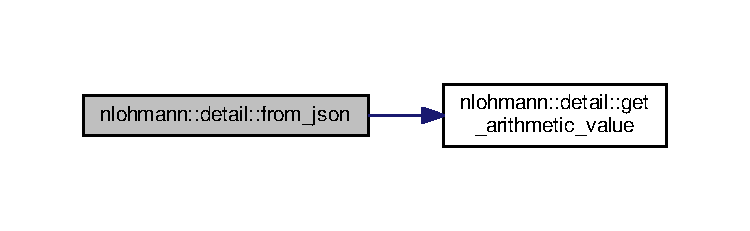
\includegraphics[width=350pt]{namespacenlohmann_1_1detail_a7cb5dd7d46a60e65f9a8e0873b3f7dd8_cgraph}
\end{center}
\end{figure}
\mbox{\Hypertarget{namespacenlohmann_1_1detail_ace4d5680ba413d9fd897ccb5d9c61a1c}\label{namespacenlohmann_1_1detail_ace4d5680ba413d9fd897ccb5d9c61a1c}} 
\index{nlohmann\+::detail@{nlohmann\+::detail}!from\+\_\+json@{from\+\_\+json}}
\index{from\+\_\+json@{from\+\_\+json}!nlohmann\+::detail@{nlohmann\+::detail}}
\subsubsection{\texorpdfstring{from\+\_\+json()}{from\_json()}\hspace{0.1cm}{\footnotesize\ttfamily [4/11]}}
{\footnotesize\ttfamily template$<$typename Basic\+Json\+Type $>$ \\
void nlohmann\+::detail\+::from\+\_\+json (\begin{DoxyParamCaption}\item[{const Basic\+Json\+Type \&}]{j,  }\item[{typename Basic\+Json\+Type\+::number\+\_\+unsigned\+\_\+t \&}]{val }\end{DoxyParamCaption})}

Here is the call graph for this function\+:\nopagebreak
\begin{figure}[H]
\begin{center}
\leavevmode
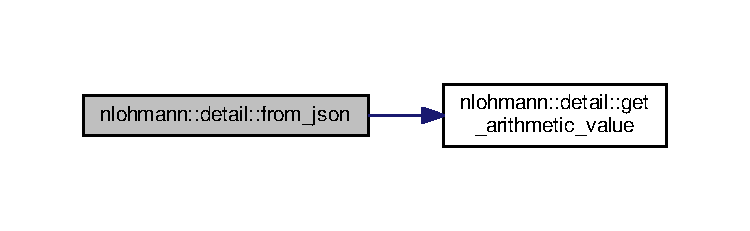
\includegraphics[width=350pt]{namespacenlohmann_1_1detail_ace4d5680ba413d9fd897ccb5d9c61a1c_cgraph}
\end{center}
\end{figure}
\mbox{\Hypertarget{namespacenlohmann_1_1detail_a047d881e611fcac709dc318f730a1732}\label{namespacenlohmann_1_1detail_a047d881e611fcac709dc318f730a1732}} 
\index{nlohmann\+::detail@{nlohmann\+::detail}!from\+\_\+json@{from\+\_\+json}}
\index{from\+\_\+json@{from\+\_\+json}!nlohmann\+::detail@{nlohmann\+::detail}}
\subsubsection{\texorpdfstring{from\+\_\+json()}{from\_json()}\hspace{0.1cm}{\footnotesize\ttfamily [5/11]}}
{\footnotesize\ttfamily template$<$typename Basic\+Json\+Type $>$ \\
void nlohmann\+::detail\+::from\+\_\+json (\begin{DoxyParamCaption}\item[{const Basic\+Json\+Type \&}]{j,  }\item[{typename Basic\+Json\+Type\+::number\+\_\+integer\+\_\+t \&}]{val }\end{DoxyParamCaption})}

Here is the call graph for this function\+:\nopagebreak
\begin{figure}[H]
\begin{center}
\leavevmode
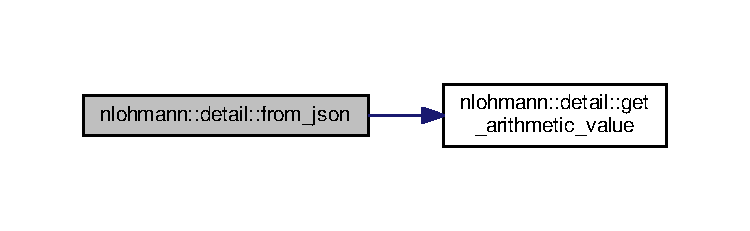
\includegraphics[width=350pt]{namespacenlohmann_1_1detail_a047d881e611fcac709dc318f730a1732_cgraph}
\end{center}
\end{figure}
\mbox{\Hypertarget{namespacenlohmann_1_1detail_acf8dd944c2c7455880dee6f0b355aa01}\label{namespacenlohmann_1_1detail_acf8dd944c2c7455880dee6f0b355aa01}} 
\index{nlohmann\+::detail@{nlohmann\+::detail}!from\+\_\+json@{from\+\_\+json}}
\index{from\+\_\+json@{from\+\_\+json}!nlohmann\+::detail@{nlohmann\+::detail}}
\subsubsection{\texorpdfstring{from\+\_\+json()}{from\_json()}\hspace{0.1cm}{\footnotesize\ttfamily [6/11]}}
{\footnotesize\ttfamily template$<$typename Basic\+Json\+Type , typename Unscoped\+Enum\+Type , enable\+\_\+if\+\_\+t$<$ is\+\_\+unscoped\+\_\+enum$<$ Unscoped\+Enum\+Type $>$\+::value, int $>$  = 0$>$ \\
void nlohmann\+::detail\+::from\+\_\+json (\begin{DoxyParamCaption}\item[{const Basic\+Json\+Type \&}]{j,  }\item[{Unscoped\+Enum\+Type \&}]{e }\end{DoxyParamCaption})}

Here is the call graph for this function\+:\nopagebreak
\begin{figure}[H]
\begin{center}
\leavevmode
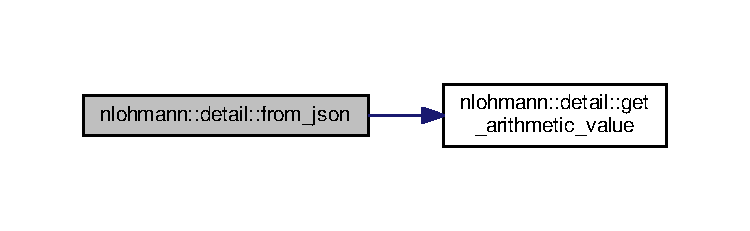
\includegraphics[width=350pt]{namespacenlohmann_1_1detail_acf8dd944c2c7455880dee6f0b355aa01_cgraph}
\end{center}
\end{figure}
\mbox{\Hypertarget{namespacenlohmann_1_1detail_abc62958462b916726b89f25fa381a129}\label{namespacenlohmann_1_1detail_abc62958462b916726b89f25fa381a129}} 
\index{nlohmann\+::detail@{nlohmann\+::detail}!from\+\_\+json@{from\+\_\+json}}
\index{from\+\_\+json@{from\+\_\+json}!nlohmann\+::detail@{nlohmann\+::detail}}
\subsubsection{\texorpdfstring{from\+\_\+json()}{from\_json()}\hspace{0.1cm}{\footnotesize\ttfamily [7/11]}}
{\footnotesize\ttfamily template$<$typename Basic\+Json\+Type $>$ \\
void nlohmann\+::detail\+::from\+\_\+json (\begin{DoxyParamCaption}\item[{const Basic\+Json\+Type \&}]{j,  }\item[{typename Basic\+Json\+Type\+::array\+\_\+t \&}]{arr }\end{DoxyParamCaption})}

\mbox{\Hypertarget{namespacenlohmann_1_1detail_a7fb5b5b8034d347b702d31d7fec4ecd7}\label{namespacenlohmann_1_1detail_a7fb5b5b8034d347b702d31d7fec4ecd7}} 
\index{nlohmann\+::detail@{nlohmann\+::detail}!from\+\_\+json@{from\+\_\+json}}
\index{from\+\_\+json@{from\+\_\+json}!nlohmann\+::detail@{nlohmann\+::detail}}
\subsubsection{\texorpdfstring{from\+\_\+json()}{from\_json()}\hspace{0.1cm}{\footnotesize\ttfamily [8/11]}}
{\footnotesize\ttfamily template$<$typename Basic\+Json\+Type , typename T , typename Allocator $>$ \\
void nlohmann\+::detail\+::from\+\_\+json (\begin{DoxyParamCaption}\item[{const Basic\+Json\+Type \&}]{j,  }\item[{std\+::forward\+\_\+list$<$ T, Allocator $>$ \&}]{l }\end{DoxyParamCaption})}

\mbox{\Hypertarget{namespacenlohmann_1_1detail_a8dcac00852dbe1f61d1e78135b19d428}\label{namespacenlohmann_1_1detail_a8dcac00852dbe1f61d1e78135b19d428}} 
\index{nlohmann\+::detail@{nlohmann\+::detail}!from\+\_\+json@{from\+\_\+json}}
\index{from\+\_\+json@{from\+\_\+json}!nlohmann\+::detail@{nlohmann\+::detail}}
\subsubsection{\texorpdfstring{from\+\_\+json()}{from\_json()}\hspace{0.1cm}{\footnotesize\ttfamily [9/11]}}
{\footnotesize\ttfamily template$<$typename Basic\+Json\+Type , typename Compatible\+Array\+Type , enable\+\_\+if\+\_\+t$<$ is\+\_\+compatible\+\_\+array\+\_\+type$<$ Basic\+Json\+Type, Compatible\+Array\+Type $>$\+::value and not std\+::is\+\_\+same$<$ typename Basic\+Json\+Type\+::array\+\_\+t, Compatible\+Array\+Type $>$\+::value, int $>$  = 0$>$ \\
void nlohmann\+::detail\+::from\+\_\+json (\begin{DoxyParamCaption}\item[{const Basic\+Json\+Type \&}]{j,  }\item[{Compatible\+Array\+Type \&}]{arr }\end{DoxyParamCaption})}

Here is the call graph for this function\+:\nopagebreak
\begin{figure}[H]
\begin{center}
\leavevmode
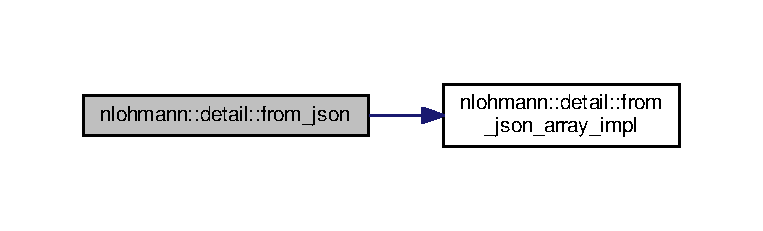
\includegraphics[width=350pt]{namespacenlohmann_1_1detail_a8dcac00852dbe1f61d1e78135b19d428_cgraph}
\end{center}
\end{figure}
\mbox{\Hypertarget{namespacenlohmann_1_1detail_a5e7a3674e8ac46f8feebad9712d7c55f}\label{namespacenlohmann_1_1detail_a5e7a3674e8ac46f8feebad9712d7c55f}} 
\index{nlohmann\+::detail@{nlohmann\+::detail}!from\+\_\+json@{from\+\_\+json}}
\index{from\+\_\+json@{from\+\_\+json}!nlohmann\+::detail@{nlohmann\+::detail}}
\subsubsection{\texorpdfstring{from\+\_\+json()}{from\_json()}\hspace{0.1cm}{\footnotesize\ttfamily [10/11]}}
{\footnotesize\ttfamily template$<$typename Basic\+Json\+Type , typename Compatible\+Object\+Type , enable\+\_\+if\+\_\+t$<$ is\+\_\+compatible\+\_\+object\+\_\+type$<$ Basic\+Json\+Type, Compatible\+Object\+Type $>$\+::value, int $>$  = 0$>$ \\
void nlohmann\+::detail\+::from\+\_\+json (\begin{DoxyParamCaption}\item[{const Basic\+Json\+Type \&}]{j,  }\item[{Compatible\+Object\+Type \&}]{obj }\end{DoxyParamCaption})}

\mbox{\Hypertarget{namespacenlohmann_1_1detail_a839b0ab50d2c9bce669068f56bc41202}\label{namespacenlohmann_1_1detail_a839b0ab50d2c9bce669068f56bc41202}} 
\index{nlohmann\+::detail@{nlohmann\+::detail}!from\+\_\+json@{from\+\_\+json}}
\index{from\+\_\+json@{from\+\_\+json}!nlohmann\+::detail@{nlohmann\+::detail}}
\subsubsection{\texorpdfstring{from\+\_\+json()}{from\_json()}\hspace{0.1cm}{\footnotesize\ttfamily [11/11]}}
{\footnotesize\ttfamily template$<$typename Basic\+Json\+Type , typename Arithmetic\+Type , enable\+\_\+if\+\_\+t$<$ std\+::is\+\_\+arithmetic$<$ Arithmetic\+Type $>$\+::value and not std\+::is\+\_\+same$<$ Arithmetic\+Type, typename Basic\+Json\+Type\+::number\+\_\+unsigned\+\_\+t $>$\+::value and not std\+::is\+\_\+same$<$ Arithmetic\+Type, typename Basic\+Json\+Type\+::number\+\_\+integer\+\_\+t $>$\+::value and not std\+::is\+\_\+same$<$ Arithmetic\+Type, typename Basic\+Json\+Type\+::number\+\_\+float\+\_\+t $>$\+::value and not std\+::is\+\_\+same$<$ Arithmetic\+Type, typename Basic\+Json\+Type\+::boolean\+\_\+t $>$\+::value, int $>$  = 0$>$ \\
void nlohmann\+::detail\+::from\+\_\+json (\begin{DoxyParamCaption}\item[{const Basic\+Json\+Type \&}]{j,  }\item[{Arithmetic\+Type \&}]{val }\end{DoxyParamCaption})}

\mbox{\Hypertarget{namespacenlohmann_1_1detail_ac53673a5ce29fb69b96d41dad33cb3b0}\label{namespacenlohmann_1_1detail_ac53673a5ce29fb69b96d41dad33cb3b0}} 
\index{nlohmann\+::detail@{nlohmann\+::detail}!from\+\_\+json\+\_\+array\+\_\+impl@{from\+\_\+json\+\_\+array\+\_\+impl}}
\index{from\+\_\+json\+\_\+array\+\_\+impl@{from\+\_\+json\+\_\+array\+\_\+impl}!nlohmann\+::detail@{nlohmann\+::detail}}
\subsubsection{\texorpdfstring{from\+\_\+json\+\_\+array\+\_\+impl()}{from\_json\_array\_impl()}\hspace{0.1cm}{\footnotesize\ttfamily [1/2]}}
{\footnotesize\ttfamily template$<$typename Basic\+Json\+Type , typename Compatible\+Array\+Type $>$ \\
void nlohmann\+::detail\+::from\+\_\+json\+\_\+array\+\_\+impl (\begin{DoxyParamCaption}\item[{const Basic\+Json\+Type \&}]{j,  }\item[{Compatible\+Array\+Type \&}]{arr,  }\item[{\hyperlink{structnlohmann_1_1detail_1_1priority__tag}{priority\+\_\+tag}$<$ 0 $>$}]{ }\end{DoxyParamCaption})}

\mbox{\Hypertarget{namespacenlohmann_1_1detail_a57f93ed57254a1639087cdc316e0fb83}\label{namespacenlohmann_1_1detail_a57f93ed57254a1639087cdc316e0fb83}} 
\index{nlohmann\+::detail@{nlohmann\+::detail}!from\+\_\+json\+\_\+array\+\_\+impl@{from\+\_\+json\+\_\+array\+\_\+impl}}
\index{from\+\_\+json\+\_\+array\+\_\+impl@{from\+\_\+json\+\_\+array\+\_\+impl}!nlohmann\+::detail@{nlohmann\+::detail}}
\subsubsection{\texorpdfstring{from\+\_\+json\+\_\+array\+\_\+impl()}{from\_json\_array\_impl()}\hspace{0.1cm}{\footnotesize\ttfamily [2/2]}}
{\footnotesize\ttfamily template$<$typename Basic\+Json\+Type , typename Compatible\+Array\+Type $>$ \\
auto nlohmann\+::detail\+::from\+\_\+json\+\_\+array\+\_\+impl (\begin{DoxyParamCaption}\item[{const Basic\+Json\+Type \&}]{j,  }\item[{Compatible\+Array\+Type \&}]{arr,  }\item[{\hyperlink{structnlohmann_1_1detail_1_1priority__tag}{priority\+\_\+tag}$<$ 1 $>$}]{ }\end{DoxyParamCaption}) -\/$>$ decltype(
    arr.\+reserve(std\+::declval$<$typename Compatible\+Array\+Type\+::size\+\_\+type$>$()),
    void())
}

\mbox{\Hypertarget{namespacenlohmann_1_1detail_a85955b9c6dd31846e4b8e891f78614b6}\label{namespacenlohmann_1_1detail_a85955b9c6dd31846e4b8e891f78614b6}} 
\index{nlohmann\+::detail@{nlohmann\+::detail}!get\+\_\+arithmetic\+\_\+value@{get\+\_\+arithmetic\+\_\+value}}
\index{get\+\_\+arithmetic\+\_\+value@{get\+\_\+arithmetic\+\_\+value}!nlohmann\+::detail@{nlohmann\+::detail}}
\subsubsection{\texorpdfstring{get\+\_\+arithmetic\+\_\+value()}{get\_arithmetic\_value()}}
{\footnotesize\ttfamily template$<$typename Basic\+Json\+Type , typename Arithmetic\+Type , enable\+\_\+if\+\_\+t$<$ std\+::is\+\_\+arithmetic$<$ Arithmetic\+Type $>$\+::value and not std\+::is\+\_\+same$<$ Arithmetic\+Type, typename Basic\+Json\+Type\+::boolean\+\_\+t $>$\+::value, int $>$  = 0$>$ \\
void nlohmann\+::detail\+::get\+\_\+arithmetic\+\_\+value (\begin{DoxyParamCaption}\item[{const Basic\+Json\+Type \&}]{j,  }\item[{Arithmetic\+Type \&}]{val }\end{DoxyParamCaption})}

\mbox{\Hypertarget{namespacenlohmann_1_1detail_a7b2601c238073c43a07862768b319cf8}\label{namespacenlohmann_1_1detail_a7b2601c238073c43a07862768b319cf8}} 
\index{nlohmann\+::detail@{nlohmann\+::detail}!N\+L\+O\+H\+M\+A\+N\+N\+\_\+\+J\+S\+O\+N\+\_\+\+H\+A\+S\+\_\+\+H\+E\+L\+P\+ER@{N\+L\+O\+H\+M\+A\+N\+N\+\_\+\+J\+S\+O\+N\+\_\+\+H\+A\+S\+\_\+\+H\+E\+L\+P\+ER}}
\index{N\+L\+O\+H\+M\+A\+N\+N\+\_\+\+J\+S\+O\+N\+\_\+\+H\+A\+S\+\_\+\+H\+E\+L\+P\+ER@{N\+L\+O\+H\+M\+A\+N\+N\+\_\+\+J\+S\+O\+N\+\_\+\+H\+A\+S\+\_\+\+H\+E\+L\+P\+ER}!nlohmann\+::detail@{nlohmann\+::detail}}
\subsubsection{\texorpdfstring{N\+L\+O\+H\+M\+A\+N\+N\+\_\+\+J\+S\+O\+N\+\_\+\+H\+A\+S\+\_\+\+H\+E\+L\+P\+E\+R()}{NLOHMANN\_JSON\_HAS\_HELPER()}\hspace{0.1cm}{\footnotesize\ttfamily [1/4]}}
{\footnotesize\ttfamily nlohmann\+::detail\+::\+N\+L\+O\+H\+M\+A\+N\+N\+\_\+\+J\+S\+O\+N\+\_\+\+H\+A\+S\+\_\+\+H\+E\+L\+P\+ER (\begin{DoxyParamCaption}\item[{mapped\+\_\+type}]{ }\end{DoxyParamCaption})}

\mbox{\Hypertarget{namespacenlohmann_1_1detail_ad19328f0c4ffe2890ecafb7c89e0355b}\label{namespacenlohmann_1_1detail_ad19328f0c4ffe2890ecafb7c89e0355b}} 
\index{nlohmann\+::detail@{nlohmann\+::detail}!N\+L\+O\+H\+M\+A\+N\+N\+\_\+\+J\+S\+O\+N\+\_\+\+H\+A\+S\+\_\+\+H\+E\+L\+P\+ER@{N\+L\+O\+H\+M\+A\+N\+N\+\_\+\+J\+S\+O\+N\+\_\+\+H\+A\+S\+\_\+\+H\+E\+L\+P\+ER}}
\index{N\+L\+O\+H\+M\+A\+N\+N\+\_\+\+J\+S\+O\+N\+\_\+\+H\+A\+S\+\_\+\+H\+E\+L\+P\+ER@{N\+L\+O\+H\+M\+A\+N\+N\+\_\+\+J\+S\+O\+N\+\_\+\+H\+A\+S\+\_\+\+H\+E\+L\+P\+ER}!nlohmann\+::detail@{nlohmann\+::detail}}
\subsubsection{\texorpdfstring{N\+L\+O\+H\+M\+A\+N\+N\+\_\+\+J\+S\+O\+N\+\_\+\+H\+A\+S\+\_\+\+H\+E\+L\+P\+E\+R()}{NLOHMANN\_JSON\_HAS\_HELPER()}\hspace{0.1cm}{\footnotesize\ttfamily [2/4]}}
{\footnotesize\ttfamily nlohmann\+::detail\+::\+N\+L\+O\+H\+M\+A\+N\+N\+\_\+\+J\+S\+O\+N\+\_\+\+H\+A\+S\+\_\+\+H\+E\+L\+P\+ER (\begin{DoxyParamCaption}\item[{key\+\_\+type}]{ }\end{DoxyParamCaption})}

\mbox{\Hypertarget{namespacenlohmann_1_1detail_af3e900eb1e0b107c812f7babbb94e69e}\label{namespacenlohmann_1_1detail_af3e900eb1e0b107c812f7babbb94e69e}} 
\index{nlohmann\+::detail@{nlohmann\+::detail}!N\+L\+O\+H\+M\+A\+N\+N\+\_\+\+J\+S\+O\+N\+\_\+\+H\+A\+S\+\_\+\+H\+E\+L\+P\+ER@{N\+L\+O\+H\+M\+A\+N\+N\+\_\+\+J\+S\+O\+N\+\_\+\+H\+A\+S\+\_\+\+H\+E\+L\+P\+ER}}
\index{N\+L\+O\+H\+M\+A\+N\+N\+\_\+\+J\+S\+O\+N\+\_\+\+H\+A\+S\+\_\+\+H\+E\+L\+P\+ER@{N\+L\+O\+H\+M\+A\+N\+N\+\_\+\+J\+S\+O\+N\+\_\+\+H\+A\+S\+\_\+\+H\+E\+L\+P\+ER}!nlohmann\+::detail@{nlohmann\+::detail}}
\subsubsection{\texorpdfstring{N\+L\+O\+H\+M\+A\+N\+N\+\_\+\+J\+S\+O\+N\+\_\+\+H\+A\+S\+\_\+\+H\+E\+L\+P\+E\+R()}{NLOHMANN\_JSON\_HAS\_HELPER()}\hspace{0.1cm}{\footnotesize\ttfamily [3/4]}}
{\footnotesize\ttfamily nlohmann\+::detail\+::\+N\+L\+O\+H\+M\+A\+N\+N\+\_\+\+J\+S\+O\+N\+\_\+\+H\+A\+S\+\_\+\+H\+E\+L\+P\+ER (\begin{DoxyParamCaption}\item[{value\+\_\+type}]{ }\end{DoxyParamCaption})}

\mbox{\Hypertarget{namespacenlohmann_1_1detail_a6648328c4b1466fdc48f1fcfbff23e2f}\label{namespacenlohmann_1_1detail_a6648328c4b1466fdc48f1fcfbff23e2f}} 
\index{nlohmann\+::detail@{nlohmann\+::detail}!N\+L\+O\+H\+M\+A\+N\+N\+\_\+\+J\+S\+O\+N\+\_\+\+H\+A\+S\+\_\+\+H\+E\+L\+P\+ER@{N\+L\+O\+H\+M\+A\+N\+N\+\_\+\+J\+S\+O\+N\+\_\+\+H\+A\+S\+\_\+\+H\+E\+L\+P\+ER}}
\index{N\+L\+O\+H\+M\+A\+N\+N\+\_\+\+J\+S\+O\+N\+\_\+\+H\+A\+S\+\_\+\+H\+E\+L\+P\+ER@{N\+L\+O\+H\+M\+A\+N\+N\+\_\+\+J\+S\+O\+N\+\_\+\+H\+A\+S\+\_\+\+H\+E\+L\+P\+ER}!nlohmann\+::detail@{nlohmann\+::detail}}
\subsubsection{\texorpdfstring{N\+L\+O\+H\+M\+A\+N\+N\+\_\+\+J\+S\+O\+N\+\_\+\+H\+A\+S\+\_\+\+H\+E\+L\+P\+E\+R()}{NLOHMANN\_JSON\_HAS\_HELPER()}\hspace{0.1cm}{\footnotesize\ttfamily [4/4]}}
{\footnotesize\ttfamily nlohmann\+::detail\+::\+N\+L\+O\+H\+M\+A\+N\+N\+\_\+\+J\+S\+O\+N\+\_\+\+H\+A\+S\+\_\+\+H\+E\+L\+P\+ER (\begin{DoxyParamCaption}\item[{iterator}]{ }\end{DoxyParamCaption})}

\mbox{\Hypertarget{namespacenlohmann_1_1detail_a09169efff3bd1771fff29bd92cea19e0}\label{namespacenlohmann_1_1detail_a09169efff3bd1771fff29bd92cea19e0}} 
\index{nlohmann\+::detail@{nlohmann\+::detail}!operator$<$@{operator$<$}}
\index{operator$<$@{operator$<$}!nlohmann\+::detail@{nlohmann\+::detail}}
\subsubsection{\texorpdfstring{operator$<$()}{operator<()}}
{\footnotesize\ttfamily bool nlohmann\+::detail\+::operator$<$ (\begin{DoxyParamCaption}\item[{const \hyperlink{namespacenlohmann_1_1detail_a90aa5ef615aa8305e9ea20d8a947980f}{value\+\_\+t}}]{lhs,  }\item[{const \hyperlink{namespacenlohmann_1_1detail_a90aa5ef615aa8305e9ea20d8a947980f}{value\+\_\+t}}]{rhs }\end{DoxyParamCaption})\hspace{0.3cm}{\ttfamily [inline]}, {\ttfamily [noexcept]}}



comparison operator for J\+S\+ON types 

Returns an ordering that is similar to Python\+:
\begin{DoxyItemize}
\item order\+: null $<$ boolean $<$ number $<$ object $<$ array $<$ string
\item furthermore, each type is not smaller than itself
\end{DoxyItemize}

\begin{DoxySince}{Since}
version 1.\+0.\+0 
\end{DoxySince}
\mbox{\Hypertarget{namespacenlohmann_1_1detail_a1a804b98cbe89b7e44b698f2ca860490}\label{namespacenlohmann_1_1detail_a1a804b98cbe89b7e44b698f2ca860490}} 
\index{nlohmann\+::detail@{nlohmann\+::detail}!to\+\_\+json@{to\+\_\+json}}
\index{to\+\_\+json@{to\+\_\+json}!nlohmann\+::detail@{nlohmann\+::detail}}
\subsubsection{\texorpdfstring{to\+\_\+json()}{to\_json()}\hspace{0.1cm}{\footnotesize\ttfamily [1/8]}}
{\footnotesize\ttfamily template$<$typename Basic\+Json\+Type , typename T , enable\+\_\+if\+\_\+t$<$ std\+::is\+\_\+same$<$ T, typename Basic\+Json\+Type\+::boolean\+\_\+t $>$\+::value, int $>$  = 0$>$ \\
void nlohmann\+::detail\+::to\+\_\+json (\begin{DoxyParamCaption}\item[{Basic\+Json\+Type \&}]{j,  }\item[{T}]{b }\end{DoxyParamCaption})\hspace{0.3cm}{\ttfamily [noexcept]}}

\mbox{\Hypertarget{namespacenlohmann_1_1detail_a7356ed05cdbbb080cee80e1211e1c6c9}\label{namespacenlohmann_1_1detail_a7356ed05cdbbb080cee80e1211e1c6c9}} 
\index{nlohmann\+::detail@{nlohmann\+::detail}!to\+\_\+json@{to\+\_\+json}}
\index{to\+\_\+json@{to\+\_\+json}!nlohmann\+::detail@{nlohmann\+::detail}}
\subsubsection{\texorpdfstring{to\+\_\+json()}{to\_json()}\hspace{0.1cm}{\footnotesize\ttfamily [2/8]}}
{\footnotesize\ttfamily template$<$typename Basic\+Json\+Type , typename Compatible\+String , enable\+\_\+if\+\_\+t$<$ std\+::is\+\_\+constructible$<$ typename Basic\+Json\+Type\+::string\+\_\+t, Compatible\+String $>$\+::value, int $>$  = 0$>$ \\
void nlohmann\+::detail\+::to\+\_\+json (\begin{DoxyParamCaption}\item[{Basic\+Json\+Type \&}]{j,  }\item[{const Compatible\+String \&}]{s }\end{DoxyParamCaption})}

\mbox{\Hypertarget{namespacenlohmann_1_1detail_a22bffdc8bc7e43af380ba2050696b230}\label{namespacenlohmann_1_1detail_a22bffdc8bc7e43af380ba2050696b230}} 
\index{nlohmann\+::detail@{nlohmann\+::detail}!to\+\_\+json@{to\+\_\+json}}
\index{to\+\_\+json@{to\+\_\+json}!nlohmann\+::detail@{nlohmann\+::detail}}
\subsubsection{\texorpdfstring{to\+\_\+json()}{to\_json()}\hspace{0.1cm}{\footnotesize\ttfamily [3/8]}}
{\footnotesize\ttfamily template$<$typename Basic\+Json\+Type , typename Float\+Type , enable\+\_\+if\+\_\+t$<$ std\+::is\+\_\+floating\+\_\+point$<$ Float\+Type $>$\+::value, int $>$  = 0$>$ \\
void nlohmann\+::detail\+::to\+\_\+json (\begin{DoxyParamCaption}\item[{Basic\+Json\+Type \&}]{j,  }\item[{Float\+Type}]{val }\end{DoxyParamCaption})\hspace{0.3cm}{\ttfamily [noexcept]}}

\mbox{\Hypertarget{namespacenlohmann_1_1detail_ae5fd66b5517b3b5a6c6b9fd9f29ba8dc}\label{namespacenlohmann_1_1detail_ae5fd66b5517b3b5a6c6b9fd9f29ba8dc}} 
\index{nlohmann\+::detail@{nlohmann\+::detail}!to\+\_\+json@{to\+\_\+json}}
\index{to\+\_\+json@{to\+\_\+json}!nlohmann\+::detail@{nlohmann\+::detail}}
\subsubsection{\texorpdfstring{to\+\_\+json()}{to\_json()}\hspace{0.1cm}{\footnotesize\ttfamily [4/8]}}
{\footnotesize\ttfamily template$<$typename Basic\+Json\+Type , typename Compatible\+Number\+Unsigned\+Type , enable\+\_\+if\+\_\+t$<$ is\+\_\+compatible\+\_\+integer\+\_\+type$<$ typename Basic\+Json\+Type\+::number\+\_\+unsigned\+\_\+t, Compatible\+Number\+Unsigned\+Type $>$\+::value, int $>$  = 0$>$ \\
void nlohmann\+::detail\+::to\+\_\+json (\begin{DoxyParamCaption}\item[{Basic\+Json\+Type \&}]{j,  }\item[{Compatible\+Number\+Unsigned\+Type}]{val }\end{DoxyParamCaption})\hspace{0.3cm}{\ttfamily [noexcept]}}

\mbox{\Hypertarget{namespacenlohmann_1_1detail_a91fe576be579c8c2fdd14610605c6dd2}\label{namespacenlohmann_1_1detail_a91fe576be579c8c2fdd14610605c6dd2}} 
\index{nlohmann\+::detail@{nlohmann\+::detail}!to\+\_\+json@{to\+\_\+json}}
\index{to\+\_\+json@{to\+\_\+json}!nlohmann\+::detail@{nlohmann\+::detail}}
\subsubsection{\texorpdfstring{to\+\_\+json()}{to\_json()}\hspace{0.1cm}{\footnotesize\ttfamily [5/8]}}
{\footnotesize\ttfamily template$<$typename Basic\+Json\+Type , typename Compatible\+Number\+Integer\+Type , enable\+\_\+if\+\_\+t$<$ is\+\_\+compatible\+\_\+integer\+\_\+type$<$ typename Basic\+Json\+Type\+::number\+\_\+integer\+\_\+t, Compatible\+Number\+Integer\+Type $>$\+::value, int $>$  = 0$>$ \\
void nlohmann\+::detail\+::to\+\_\+json (\begin{DoxyParamCaption}\item[{Basic\+Json\+Type \&}]{j,  }\item[{Compatible\+Number\+Integer\+Type}]{val }\end{DoxyParamCaption})\hspace{0.3cm}{\ttfamily [noexcept]}}

\mbox{\Hypertarget{namespacenlohmann_1_1detail_a1f83504de38ee6f440a77ae898b86a18}\label{namespacenlohmann_1_1detail_a1f83504de38ee6f440a77ae898b86a18}} 
\index{nlohmann\+::detail@{nlohmann\+::detail}!to\+\_\+json@{to\+\_\+json}}
\index{to\+\_\+json@{to\+\_\+json}!nlohmann\+::detail@{nlohmann\+::detail}}
\subsubsection{\texorpdfstring{to\+\_\+json()}{to\_json()}\hspace{0.1cm}{\footnotesize\ttfamily [6/8]}}
{\footnotesize\ttfamily template$<$typename Basic\+Json\+Type , typename Unscoped\+Enum\+Type , enable\+\_\+if\+\_\+t$<$ is\+\_\+unscoped\+\_\+enum$<$ Unscoped\+Enum\+Type $>$\+::value, int $>$  = 0$>$ \\
void nlohmann\+::detail\+::to\+\_\+json (\begin{DoxyParamCaption}\item[{Basic\+Json\+Type \&}]{j,  }\item[{Unscoped\+Enum\+Type}]{e }\end{DoxyParamCaption})\hspace{0.3cm}{\ttfamily [noexcept]}}

\mbox{\Hypertarget{namespacenlohmann_1_1detail_a3afebc132c5ff83f9cd160e52030fdfd}\label{namespacenlohmann_1_1detail_a3afebc132c5ff83f9cd160e52030fdfd}} 
\index{nlohmann\+::detail@{nlohmann\+::detail}!to\+\_\+json@{to\+\_\+json}}
\index{to\+\_\+json@{to\+\_\+json}!nlohmann\+::detail@{nlohmann\+::detail}}
\subsubsection{\texorpdfstring{to\+\_\+json()}{to\_json()}\hspace{0.1cm}{\footnotesize\ttfamily [7/8]}}
{\footnotesize\ttfamily template$<$typename Basic\+Json\+Type , typename Compatible\+Array\+Type , enable\+\_\+if\+\_\+t$<$ is\+\_\+compatible\+\_\+array\+\_\+type$<$ Basic\+Json\+Type, Compatible\+Array\+Type $>$\+::value or std\+::is\+\_\+same$<$ typename Basic\+Json\+Type\+::array\+\_\+t, Compatible\+Array\+Type $>$\+::value, int $>$  = 0$>$ \\
void nlohmann\+::detail\+::to\+\_\+json (\begin{DoxyParamCaption}\item[{Basic\+Json\+Type \&}]{j,  }\item[{const Compatible\+Array\+Type \&}]{arr }\end{DoxyParamCaption})}

\mbox{\Hypertarget{namespacenlohmann_1_1detail_a6fa2f784014bfc0b62d7a35d51e676c9}\label{namespacenlohmann_1_1detail_a6fa2f784014bfc0b62d7a35d51e676c9}} 
\index{nlohmann\+::detail@{nlohmann\+::detail}!to\+\_\+json@{to\+\_\+json}}
\index{to\+\_\+json@{to\+\_\+json}!nlohmann\+::detail@{nlohmann\+::detail}}
\subsubsection{\texorpdfstring{to\+\_\+json()}{to\_json()}\hspace{0.1cm}{\footnotesize\ttfamily [8/8]}}
{\footnotesize\ttfamily template$<$typename Basic\+Json\+Type , typename Compatible\+Object\+Type , enable\+\_\+if\+\_\+t$<$ is\+\_\+compatible\+\_\+object\+\_\+type$<$ Basic\+Json\+Type, Compatible\+Object\+Type $>$\+::value, int $>$  = 0$>$ \\
void nlohmann\+::detail\+::to\+\_\+json (\begin{DoxyParamCaption}\item[{Basic\+Json\+Type \&}]{j,  }\item[{const Compatible\+Object\+Type \&}]{arr }\end{DoxyParamCaption})}


\hypertarget{namespaceshaan97}{}\section{shaan97 Namespace Reference}
\label{namespaceshaan97}\index{shaan97@{shaan97}}


The namespace for the github user \hyperlink{namespaceshaan97}{shaan97}.  


\subsection*{Namespaces}
\begin{DoxyCompactItemize}
\item 
 \hyperlink{namespaceshaan97_1_1sync}{sync}
\begin{DoxyCompactList}\small\item\em The namespace for the sync project. \end{DoxyCompactList}\end{DoxyCompactItemize}


\subsection{Detailed Description}
The namespace for the github user \hyperlink{namespaceshaan97}{shaan97}. 
\hypertarget{namespaceshaan97_1_1sync}{}\section{shaan97\+:\+:sync Namespace Reference}
\label{namespaceshaan97_1_1sync}\index{shaan97\+::sync@{shaan97\+::sync}}


The namespace for the sync project.  


\subsection*{Classes}
\begin{DoxyCompactItemize}
\item 
class \hyperlink{classshaan97_1_1sync_1_1_client}{Client}
\item 
class \hyperlink{classshaan97_1_1sync_1_1_error}{Error}
\item 
class \hyperlink{classshaan97_1_1sync_1_1_group}{Group}
\item 
class \hyperlink{classshaan97_1_1sync_1_1_member}{Member}
\begin{DoxyCompactList}\small\item\em {\ttfamily \hyperlink{classshaan97_1_1sync_1_1_member}{Member}}s are always members of a {\ttfamily \hyperlink{classshaan97_1_1sync_1_1_group}{shaan97\+::sync\+::\+Group}}. They are the means of sending and receiving data from clients. \end{DoxyCompactList}\item 
struct \hyperlink{structshaan97_1_1sync_1_1_message}{Message}
\item 
class \hyperlink{classshaan97_1_1sync_1_1_server}{Server}
\end{DoxyCompactItemize}
\subsection*{Typedefs}
\begin{DoxyCompactItemize}
\item 
typedef std\+::string \hyperlink{namespaceshaan97_1_1sync_a34cebf175d27dfc3d82f24608f7043c1}{G\+R\+O\+U\+P\+\_\+\+ID}
\item 
typedef std\+::string \hyperlink{namespaceshaan97_1_1sync_af59c2c9185f7cde547b79fbe0bf8ec71}{Member\+Name}
\end{DoxyCompactItemize}
\subsection*{Enumerations}
\begin{DoxyCompactItemize}
\item 
enum \hyperlink{namespaceshaan97_1_1sync_a69f4d5572314be52626f6a1c8ecc8db9}{E\+R\+R\+O\+R\+\_\+\+T\+Y\+PE} \{ \newline
\hyperlink{namespaceshaan97_1_1sync_a69f4d5572314be52626f6a1c8ecc8db9a52c4a0d7144160a041261253a2a82894}{N\+O\+NE} = 0, 
\hyperlink{namespaceshaan97_1_1sync_a69f4d5572314be52626f6a1c8ecc8db9a826ca9fbc231462e0dae956a8fdc078b}{F\+A\+I\+L\+E\+D\+\_\+\+C\+O\+N\+N\+E\+C\+T\+I\+ON}, 
\hyperlink{namespaceshaan97_1_1sync_a69f4d5572314be52626f6a1c8ecc8db9ac6c293b7f0506d3ee58658539e4e3fc0}{G\+I\+D\+\_\+\+E\+X\+I\+S\+TS}, 
\hyperlink{namespaceshaan97_1_1sync_a69f4d5572314be52626f6a1c8ecc8db9af4f2e82194c014add58de880aeb14bee}{G\+I\+D\+\_\+\+N\+O\+\_\+\+E\+X\+I\+ST}, 
\newline
\hyperlink{namespaceshaan97_1_1sync_a69f4d5572314be52626f6a1c8ecc8db9a8fce264c2465f8d142f4568a833666c7}{O\+T\+H\+ER}, 
\hyperlink{namespaceshaan97_1_1sync_a69f4d5572314be52626f6a1c8ecc8db9ab01cc23469df9566321a2dbfe95283eb}{A\+C\+C\+E\+S\+S\+\_\+\+D\+E\+N\+I\+ED}, 
\hyperlink{namespaceshaan97_1_1sync_a69f4d5572314be52626f6a1c8ecc8db9aa848eafa9f1a60215e209859d3e687c4}{C\+O\+R\+R\+U\+P\+T\+E\+D\+\_\+\+D\+A\+TA}, 
\hyperlink{namespaceshaan97_1_1sync_a69f4d5572314be52626f6a1c8ecc8db9a54f2deaea47604a5b0f6bc7b4e059e83}{M\+E\+M\+B\+E\+R\+\_\+\+E\+X\+I\+S\+TS}, 
\newline
\hyperlink{namespaceshaan97_1_1sync_a69f4d5572314be52626f6a1c8ecc8db9a240795385057c568d066e43d08c5c240}{M\+E\+M\+B\+E\+R\+\_\+\+N\+O\+\_\+\+E\+X\+I\+ST}
 \}
\item 
enum \hyperlink{namespaceshaan97_1_1sync_a902024d98481afc28794167b4524f537}{Message\+Type} \{ \newline
\hyperlink{namespaceshaan97_1_1sync_a902024d98481afc28794167b4524f537a04edc961a82f770aec6cb525f6d3e7e9}{G\+R\+O\+U\+P\+\_\+\+J\+O\+IN} = 0, 
\hyperlink{namespaceshaan97_1_1sync_a902024d98481afc28794167b4524f537ad852dfe5f29536b5807099fd5265d1ae}{G\+R\+O\+U\+P\+\_\+\+C\+R\+E\+A\+TE}, 
\hyperlink{namespaceshaan97_1_1sync_a902024d98481afc28794167b4524f537a3d97f8aa67f41502d7761df9815eb7f0}{H\+E\+A\+R\+T\+B\+E\+AT}, 
\hyperlink{namespaceshaan97_1_1sync_a902024d98481afc28794167b4524f537a8aea50566a25675d0046705e9c248521}{G\+R\+O\+U\+P\+\_\+\+E\+X\+IT}, 
\newline
\hyperlink{namespaceshaan97_1_1sync_a902024d98481afc28794167b4524f537a22f6cfdf41b7ddebad7ddccfb0e53980}{P\+R\+O\+M\+O\+TE}, 
\hyperlink{namespaceshaan97_1_1sync_a902024d98481afc28794167b4524f537a8d7c77c6567e71e9b955fa852ba29878}{E\+R\+R\+OR}
 \}
\item 
enum \hyperlink{namespaceshaan97_1_1sync_a475934f59b3e5af2cfdab7cd20942b6c}{J\+S\+O\+N\+\_\+\+K\+EY} \{ \newline
\hyperlink{namespaceshaan97_1_1sync_a475934f59b3e5af2cfdab7cd20942b6ca6c529427f3e126f6d61d2554857fc00d}{T\+Y\+PE} = 0, 
\hyperlink{namespaceshaan97_1_1sync_a475934f59b3e5af2cfdab7cd20942b6ca7e90cbf50da3205840833faa1093d520}{M\+E\+M\+B\+ER}, 
\hyperlink{namespaceshaan97_1_1sync_a475934f59b3e5af2cfdab7cd20942b6ca1a66b3a888f6bc7c1ab901824009f47c}{G\+ID}, 
\hyperlink{namespaceshaan97_1_1sync_a475934f59b3e5af2cfdab7cd20942b6ca862ce1ab3824757a5fd158575bb693a2}{O\+T\+H\+E\+R\+\_\+\+M\+EM}, 
\newline
\hyperlink{namespaceshaan97_1_1sync_a475934f59b3e5af2cfdab7cd20942b6ca9d51e87b2491fb0fd052b0d26cd3225d}{N\+A\+ME}, 
\hyperlink{namespaceshaan97_1_1sync_a475934f59b3e5af2cfdab7cd20942b6caa68cbff9a74544558a92a490ef0b8fd8}{E\+R\+R\+O\+R\+\_\+\+M\+E\+S\+S\+A\+GE}, 
\hyperlink{namespaceshaan97_1_1sync_a475934f59b3e5af2cfdab7cd20942b6cac8e6b57e5b75aa7001876e5f86d05db4}{D\+E\+T\+A\+I\+LS}, 
\hyperlink{namespaceshaan97_1_1sync_a475934f59b3e5af2cfdab7cd20942b6ca80ede7efddbd087b6d9e11798ccf2d38}{S\+Y\+N\+C\+\_\+\+E\+R\+R\+OR}, 
\newline
\hyperlink{namespaceshaan97_1_1sync_a475934f59b3e5af2cfdab7cd20942b6cae63eff52102acea6456a316714833c9b}{B\+O\+O\+S\+T\+\_\+\+E\+R\+R\+OR}
 \}
\end{DoxyCompactItemize}
\subsection*{Functions}
\begin{DoxyCompactItemize}
\item 
std\+::ostream \& \hyperlink{namespaceshaan97_1_1sync_a734625a59747d9c85857e245a8975bb9}{operator$<$$<$} (std\+::ostream \&out, const \hyperlink{classshaan97_1_1sync_1_1_error}{Error} \&e)
\item 
void \hyperlink{namespaceshaan97_1_1sync_a6ccb9e98c182a3bac3ee37ad64f76bbc}{to\+\_\+json} (\hyperlink{namespacenlohmann_a2bfd99e845a2e5cd90aeaf1b1431f474}{nlohmann\+::json} \&j, const \hyperlink{classshaan97_1_1sync_1_1_error}{Error} \&e)
\item 
void \hyperlink{namespaceshaan97_1_1sync_a9e374973ba3aed17d32efd550318c94c}{from\+\_\+json} (\hyperlink{namespacenlohmann_a2bfd99e845a2e5cd90aeaf1b1431f474}{nlohmann\+::json} \&j, \hyperlink{classshaan97_1_1sync_1_1_error}{Error} \&e)
\item 
void \hyperlink{group___serialization_gaad90c8bd50725f5382dc2207225f52ee}{to\+\_\+json} (\hyperlink{namespacenlohmann_a2bfd99e845a2e5cd90aeaf1b1431f474}{nlohmann\+::json} \&j, const \hyperlink{classshaan97_1_1sync_1_1_member}{Member} \&m)
\item 
void \hyperlink{group___serialization_ga35dd3deb42a1ec52e00a2980b5c7c842}{from\+\_\+json} (\hyperlink{namespacenlohmann_a2bfd99e845a2e5cd90aeaf1b1431f474}{nlohmann\+::json} \&j, \hyperlink{classshaan97_1_1sync_1_1_member}{Member} \&m)
\item 
void \hyperlink{group___serialization_ga213581ca789d5151c699fb4cb30db916}{to\+\_\+json} (\hyperlink{namespacenlohmann_a2bfd99e845a2e5cd90aeaf1b1431f474}{nlohmann\+::json} \&j, const \hyperlink{structshaan97_1_1sync_1_1_message}{Message} \&m)
\begin{DoxyCompactList}\small\item\em Converts a {\ttfamily \hyperlink{structshaan97_1_1sync_1_1_message}{Message}} into a {\ttfamily \hyperlink{namespacenlohmann_a2bfd99e845a2e5cd90aeaf1b1431f474}{nlohmann\+::json} object} \end{DoxyCompactList}\item 
void \hyperlink{group___serialization_gaba06015bb8b13049b093f0bde8e89377}{from\+\_\+json} (\hyperlink{namespacenlohmann_a2bfd99e845a2e5cd90aeaf1b1431f474}{nlohmann\+::json} \&j, \hyperlink{structshaan97_1_1sync_1_1_message}{Message} \&m)
\begin{DoxyCompactList}\small\item\em Converts a {\ttfamily \hyperlink{namespacenlohmann_a2bfd99e845a2e5cd90aeaf1b1431f474}{nlohmann\+::json}} into a {\ttfamily \hyperlink{structshaan97_1_1sync_1_1_message}{Message}} object. \end{DoxyCompactList}\end{DoxyCompactItemize}


\subsection{Detailed Description}
The namespace for the sync project. 

\subsection{Typedef Documentation}
\mbox{\Hypertarget{namespaceshaan97_1_1sync_a34cebf175d27dfc3d82f24608f7043c1}\label{namespaceshaan97_1_1sync_a34cebf175d27dfc3d82f24608f7043c1}} 
\index{shaan97\+::sync@{shaan97\+::sync}!G\+R\+O\+U\+P\+\_\+\+ID@{G\+R\+O\+U\+P\+\_\+\+ID}}
\index{G\+R\+O\+U\+P\+\_\+\+ID@{G\+R\+O\+U\+P\+\_\+\+ID}!shaan97\+::sync@{shaan97\+::sync}}
\subsubsection{\texorpdfstring{G\+R\+O\+U\+P\+\_\+\+ID}{GROUP\_ID}}
{\footnotesize\ttfamily typedef std\+::string \hyperlink{namespaceshaan97_1_1sync_a34cebf175d27dfc3d82f24608f7043c1}{shaan97\+::sync\+::\+G\+R\+O\+U\+P\+\_\+\+ID}}

\mbox{\Hypertarget{namespaceshaan97_1_1sync_af59c2c9185f7cde547b79fbe0bf8ec71}\label{namespaceshaan97_1_1sync_af59c2c9185f7cde547b79fbe0bf8ec71}} 
\index{shaan97\+::sync@{shaan97\+::sync}!Member\+Name@{Member\+Name}}
\index{Member\+Name@{Member\+Name}!shaan97\+::sync@{shaan97\+::sync}}
\subsubsection{\texorpdfstring{Member\+Name}{MemberName}}
{\footnotesize\ttfamily typedef std\+::string \hyperlink{namespaceshaan97_1_1sync_af59c2c9185f7cde547b79fbe0bf8ec71}{shaan97\+::sync\+::\+Member\+Name}}



\subsection{Enumeration Type Documentation}
\mbox{\Hypertarget{namespaceshaan97_1_1sync_a69f4d5572314be52626f6a1c8ecc8db9}\label{namespaceshaan97_1_1sync_a69f4d5572314be52626f6a1c8ecc8db9}} 
\index{shaan97\+::sync@{shaan97\+::sync}!E\+R\+R\+O\+R\+\_\+\+T\+Y\+PE@{E\+R\+R\+O\+R\+\_\+\+T\+Y\+PE}}
\index{E\+R\+R\+O\+R\+\_\+\+T\+Y\+PE@{E\+R\+R\+O\+R\+\_\+\+T\+Y\+PE}!shaan97\+::sync@{shaan97\+::sync}}
\subsubsection{\texorpdfstring{E\+R\+R\+O\+R\+\_\+\+T\+Y\+PE}{ERROR\_TYPE}}
{\footnotesize\ttfamily enum \hyperlink{namespaceshaan97_1_1sync_a69f4d5572314be52626f6a1c8ecc8db9}{shaan97\+::sync\+::\+E\+R\+R\+O\+R\+\_\+\+T\+Y\+PE}}

\begin{DoxyEnumFields}{Enumerator}
\raisebox{\heightof{T}}[0pt][0pt]{\index{N\+O\+NE@{N\+O\+NE}!shaan97\+::sync@{shaan97\+::sync}}\index{shaan97\+::sync@{shaan97\+::sync}!N\+O\+NE@{N\+O\+NE}}}\mbox{\Hypertarget{namespaceshaan97_1_1sync_a69f4d5572314be52626f6a1c8ecc8db9a52c4a0d7144160a041261253a2a82894}\label{namespaceshaan97_1_1sync_a69f4d5572314be52626f6a1c8ecc8db9a52c4a0d7144160a041261253a2a82894}} 
N\+O\+NE&\\
\hline

\raisebox{\heightof{T}}[0pt][0pt]{\index{F\+A\+I\+L\+E\+D\+\_\+\+C\+O\+N\+N\+E\+C\+T\+I\+ON@{F\+A\+I\+L\+E\+D\+\_\+\+C\+O\+N\+N\+E\+C\+T\+I\+ON}!shaan97\+::sync@{shaan97\+::sync}}\index{shaan97\+::sync@{shaan97\+::sync}!F\+A\+I\+L\+E\+D\+\_\+\+C\+O\+N\+N\+E\+C\+T\+I\+ON@{F\+A\+I\+L\+E\+D\+\_\+\+C\+O\+N\+N\+E\+C\+T\+I\+ON}}}\mbox{\Hypertarget{namespaceshaan97_1_1sync_a69f4d5572314be52626f6a1c8ecc8db9a826ca9fbc231462e0dae956a8fdc078b}\label{namespaceshaan97_1_1sync_a69f4d5572314be52626f6a1c8ecc8db9a826ca9fbc231462e0dae956a8fdc078b}} 
F\+A\+I\+L\+E\+D\+\_\+\+C\+O\+N\+N\+E\+C\+T\+I\+ON&\\
\hline

\raisebox{\heightof{T}}[0pt][0pt]{\index{G\+I\+D\+\_\+\+E\+X\+I\+S\+TS@{G\+I\+D\+\_\+\+E\+X\+I\+S\+TS}!shaan97\+::sync@{shaan97\+::sync}}\index{shaan97\+::sync@{shaan97\+::sync}!G\+I\+D\+\_\+\+E\+X\+I\+S\+TS@{G\+I\+D\+\_\+\+E\+X\+I\+S\+TS}}}\mbox{\Hypertarget{namespaceshaan97_1_1sync_a69f4d5572314be52626f6a1c8ecc8db9ac6c293b7f0506d3ee58658539e4e3fc0}\label{namespaceshaan97_1_1sync_a69f4d5572314be52626f6a1c8ecc8db9ac6c293b7f0506d3ee58658539e4e3fc0}} 
G\+I\+D\+\_\+\+E\+X\+I\+S\+TS&\\
\hline

\raisebox{\heightof{T}}[0pt][0pt]{\index{G\+I\+D\+\_\+\+N\+O\+\_\+\+E\+X\+I\+ST@{G\+I\+D\+\_\+\+N\+O\+\_\+\+E\+X\+I\+ST}!shaan97\+::sync@{shaan97\+::sync}}\index{shaan97\+::sync@{shaan97\+::sync}!G\+I\+D\+\_\+\+N\+O\+\_\+\+E\+X\+I\+ST@{G\+I\+D\+\_\+\+N\+O\+\_\+\+E\+X\+I\+ST}}}\mbox{\Hypertarget{namespaceshaan97_1_1sync_a69f4d5572314be52626f6a1c8ecc8db9af4f2e82194c014add58de880aeb14bee}\label{namespaceshaan97_1_1sync_a69f4d5572314be52626f6a1c8ecc8db9af4f2e82194c014add58de880aeb14bee}} 
G\+I\+D\+\_\+\+N\+O\+\_\+\+E\+X\+I\+ST&\\
\hline

\raisebox{\heightof{T}}[0pt][0pt]{\index{O\+T\+H\+ER@{O\+T\+H\+ER}!shaan97\+::sync@{shaan97\+::sync}}\index{shaan97\+::sync@{shaan97\+::sync}!O\+T\+H\+ER@{O\+T\+H\+ER}}}\mbox{\Hypertarget{namespaceshaan97_1_1sync_a69f4d5572314be52626f6a1c8ecc8db9a8fce264c2465f8d142f4568a833666c7}\label{namespaceshaan97_1_1sync_a69f4d5572314be52626f6a1c8ecc8db9a8fce264c2465f8d142f4568a833666c7}} 
O\+T\+H\+ER&\\
\hline

\raisebox{\heightof{T}}[0pt][0pt]{\index{A\+C\+C\+E\+S\+S\+\_\+\+D\+E\+N\+I\+ED@{A\+C\+C\+E\+S\+S\+\_\+\+D\+E\+N\+I\+ED}!shaan97\+::sync@{shaan97\+::sync}}\index{shaan97\+::sync@{shaan97\+::sync}!A\+C\+C\+E\+S\+S\+\_\+\+D\+E\+N\+I\+ED@{A\+C\+C\+E\+S\+S\+\_\+\+D\+E\+N\+I\+ED}}}\mbox{\Hypertarget{namespaceshaan97_1_1sync_a69f4d5572314be52626f6a1c8ecc8db9ab01cc23469df9566321a2dbfe95283eb}\label{namespaceshaan97_1_1sync_a69f4d5572314be52626f6a1c8ecc8db9ab01cc23469df9566321a2dbfe95283eb}} 
A\+C\+C\+E\+S\+S\+\_\+\+D\+E\+N\+I\+ED&\\
\hline

\raisebox{\heightof{T}}[0pt][0pt]{\index{C\+O\+R\+R\+U\+P\+T\+E\+D\+\_\+\+D\+A\+TA@{C\+O\+R\+R\+U\+P\+T\+E\+D\+\_\+\+D\+A\+TA}!shaan97\+::sync@{shaan97\+::sync}}\index{shaan97\+::sync@{shaan97\+::sync}!C\+O\+R\+R\+U\+P\+T\+E\+D\+\_\+\+D\+A\+TA@{C\+O\+R\+R\+U\+P\+T\+E\+D\+\_\+\+D\+A\+TA}}}\mbox{\Hypertarget{namespaceshaan97_1_1sync_a69f4d5572314be52626f6a1c8ecc8db9aa848eafa9f1a60215e209859d3e687c4}\label{namespaceshaan97_1_1sync_a69f4d5572314be52626f6a1c8ecc8db9aa848eafa9f1a60215e209859d3e687c4}} 
C\+O\+R\+R\+U\+P\+T\+E\+D\+\_\+\+D\+A\+TA&\\
\hline

\raisebox{\heightof{T}}[0pt][0pt]{\index{M\+E\+M\+B\+E\+R\+\_\+\+E\+X\+I\+S\+TS@{M\+E\+M\+B\+E\+R\+\_\+\+E\+X\+I\+S\+TS}!shaan97\+::sync@{shaan97\+::sync}}\index{shaan97\+::sync@{shaan97\+::sync}!M\+E\+M\+B\+E\+R\+\_\+\+E\+X\+I\+S\+TS@{M\+E\+M\+B\+E\+R\+\_\+\+E\+X\+I\+S\+TS}}}\mbox{\Hypertarget{namespaceshaan97_1_1sync_a69f4d5572314be52626f6a1c8ecc8db9a54f2deaea47604a5b0f6bc7b4e059e83}\label{namespaceshaan97_1_1sync_a69f4d5572314be52626f6a1c8ecc8db9a54f2deaea47604a5b0f6bc7b4e059e83}} 
M\+E\+M\+B\+E\+R\+\_\+\+E\+X\+I\+S\+TS&\\
\hline

\raisebox{\heightof{T}}[0pt][0pt]{\index{M\+E\+M\+B\+E\+R\+\_\+\+N\+O\+\_\+\+E\+X\+I\+ST@{M\+E\+M\+B\+E\+R\+\_\+\+N\+O\+\_\+\+E\+X\+I\+ST}!shaan97\+::sync@{shaan97\+::sync}}\index{shaan97\+::sync@{shaan97\+::sync}!M\+E\+M\+B\+E\+R\+\_\+\+N\+O\+\_\+\+E\+X\+I\+ST@{M\+E\+M\+B\+E\+R\+\_\+\+N\+O\+\_\+\+E\+X\+I\+ST}}}\mbox{\Hypertarget{namespaceshaan97_1_1sync_a69f4d5572314be52626f6a1c8ecc8db9a240795385057c568d066e43d08c5c240}\label{namespaceshaan97_1_1sync_a69f4d5572314be52626f6a1c8ecc8db9a240795385057c568d066e43d08c5c240}} 
M\+E\+M\+B\+E\+R\+\_\+\+N\+O\+\_\+\+E\+X\+I\+ST&\\
\hline

\end{DoxyEnumFields}
\mbox{\Hypertarget{namespaceshaan97_1_1sync_a475934f59b3e5af2cfdab7cd20942b6c}\label{namespaceshaan97_1_1sync_a475934f59b3e5af2cfdab7cd20942b6c}} 
\index{shaan97\+::sync@{shaan97\+::sync}!J\+S\+O\+N\+\_\+\+K\+EY@{J\+S\+O\+N\+\_\+\+K\+EY}}
\index{J\+S\+O\+N\+\_\+\+K\+EY@{J\+S\+O\+N\+\_\+\+K\+EY}!shaan97\+::sync@{shaan97\+::sync}}
\subsubsection{\texorpdfstring{J\+S\+O\+N\+\_\+\+K\+EY}{JSON\_KEY}}
{\footnotesize\ttfamily enum \hyperlink{namespaceshaan97_1_1sync_a475934f59b3e5af2cfdab7cd20942b6c}{shaan97\+::sync\+::\+J\+S\+O\+N\+\_\+\+K\+EY}}

All possible J\+S\+ON Key Types for our defined A\+PI \begin{DoxyEnumFields}{Enumerator}
\raisebox{\heightof{T}}[0pt][0pt]{\index{T\+Y\+PE@{T\+Y\+PE}!shaan97\+::sync@{shaan97\+::sync}}\index{shaan97\+::sync@{shaan97\+::sync}!T\+Y\+PE@{T\+Y\+PE}}}\mbox{\Hypertarget{namespaceshaan97_1_1sync_a475934f59b3e5af2cfdab7cd20942b6ca6c529427f3e126f6d61d2554857fc00d}\label{namespaceshaan97_1_1sync_a475934f59b3e5af2cfdab7cd20942b6ca6c529427f3e126f6d61d2554857fc00d}} 
T\+Y\+PE&\\
\hline

\raisebox{\heightof{T}}[0pt][0pt]{\index{M\+E\+M\+B\+ER@{M\+E\+M\+B\+ER}!shaan97\+::sync@{shaan97\+::sync}}\index{shaan97\+::sync@{shaan97\+::sync}!M\+E\+M\+B\+ER@{M\+E\+M\+B\+ER}}}\mbox{\Hypertarget{namespaceshaan97_1_1sync_a475934f59b3e5af2cfdab7cd20942b6ca7e90cbf50da3205840833faa1093d520}\label{namespaceshaan97_1_1sync_a475934f59b3e5af2cfdab7cd20942b6ca7e90cbf50da3205840833faa1093d520}} 
M\+E\+M\+B\+ER&\\
\hline

\raisebox{\heightof{T}}[0pt][0pt]{\index{G\+ID@{G\+ID}!shaan97\+::sync@{shaan97\+::sync}}\index{shaan97\+::sync@{shaan97\+::sync}!G\+ID@{G\+ID}}}\mbox{\Hypertarget{namespaceshaan97_1_1sync_a475934f59b3e5af2cfdab7cd20942b6ca1a66b3a888f6bc7c1ab901824009f47c}\label{namespaceshaan97_1_1sync_a475934f59b3e5af2cfdab7cd20942b6ca1a66b3a888f6bc7c1ab901824009f47c}} 
G\+ID&\\
\hline

\raisebox{\heightof{T}}[0pt][0pt]{\index{O\+T\+H\+E\+R\+\_\+\+M\+EM@{O\+T\+H\+E\+R\+\_\+\+M\+EM}!shaan97\+::sync@{shaan97\+::sync}}\index{shaan97\+::sync@{shaan97\+::sync}!O\+T\+H\+E\+R\+\_\+\+M\+EM@{O\+T\+H\+E\+R\+\_\+\+M\+EM}}}\mbox{\Hypertarget{namespaceshaan97_1_1sync_a475934f59b3e5af2cfdab7cd20942b6ca862ce1ab3824757a5fd158575bb693a2}\label{namespaceshaan97_1_1sync_a475934f59b3e5af2cfdab7cd20942b6ca862ce1ab3824757a5fd158575bb693a2}} 
O\+T\+H\+E\+R\+\_\+\+M\+EM&\\
\hline

\raisebox{\heightof{T}}[0pt][0pt]{\index{N\+A\+ME@{N\+A\+ME}!shaan97\+::sync@{shaan97\+::sync}}\index{shaan97\+::sync@{shaan97\+::sync}!N\+A\+ME@{N\+A\+ME}}}\mbox{\Hypertarget{namespaceshaan97_1_1sync_a475934f59b3e5af2cfdab7cd20942b6ca9d51e87b2491fb0fd052b0d26cd3225d}\label{namespaceshaan97_1_1sync_a475934f59b3e5af2cfdab7cd20942b6ca9d51e87b2491fb0fd052b0d26cd3225d}} 
N\+A\+ME&\\
\hline

\raisebox{\heightof{T}}[0pt][0pt]{\index{E\+R\+R\+O\+R\+\_\+\+M\+E\+S\+S\+A\+GE@{E\+R\+R\+O\+R\+\_\+\+M\+E\+S\+S\+A\+GE}!shaan97\+::sync@{shaan97\+::sync}}\index{shaan97\+::sync@{shaan97\+::sync}!E\+R\+R\+O\+R\+\_\+\+M\+E\+S\+S\+A\+GE@{E\+R\+R\+O\+R\+\_\+\+M\+E\+S\+S\+A\+GE}}}\mbox{\Hypertarget{namespaceshaan97_1_1sync_a475934f59b3e5af2cfdab7cd20942b6caa68cbff9a74544558a92a490ef0b8fd8}\label{namespaceshaan97_1_1sync_a475934f59b3e5af2cfdab7cd20942b6caa68cbff9a74544558a92a490ef0b8fd8}} 
E\+R\+R\+O\+R\+\_\+\+M\+E\+S\+S\+A\+GE&\\
\hline

\raisebox{\heightof{T}}[0pt][0pt]{\index{D\+E\+T\+A\+I\+LS@{D\+E\+T\+A\+I\+LS}!shaan97\+::sync@{shaan97\+::sync}}\index{shaan97\+::sync@{shaan97\+::sync}!D\+E\+T\+A\+I\+LS@{D\+E\+T\+A\+I\+LS}}}\mbox{\Hypertarget{namespaceshaan97_1_1sync_a475934f59b3e5af2cfdab7cd20942b6cac8e6b57e5b75aa7001876e5f86d05db4}\label{namespaceshaan97_1_1sync_a475934f59b3e5af2cfdab7cd20942b6cac8e6b57e5b75aa7001876e5f86d05db4}} 
D\+E\+T\+A\+I\+LS&\\
\hline

\raisebox{\heightof{T}}[0pt][0pt]{\index{S\+Y\+N\+C\+\_\+\+E\+R\+R\+OR@{S\+Y\+N\+C\+\_\+\+E\+R\+R\+OR}!shaan97\+::sync@{shaan97\+::sync}}\index{shaan97\+::sync@{shaan97\+::sync}!S\+Y\+N\+C\+\_\+\+E\+R\+R\+OR@{S\+Y\+N\+C\+\_\+\+E\+R\+R\+OR}}}\mbox{\Hypertarget{namespaceshaan97_1_1sync_a475934f59b3e5af2cfdab7cd20942b6ca80ede7efddbd087b6d9e11798ccf2d38}\label{namespaceshaan97_1_1sync_a475934f59b3e5af2cfdab7cd20942b6ca80ede7efddbd087b6d9e11798ccf2d38}} 
S\+Y\+N\+C\+\_\+\+E\+R\+R\+OR&\\
\hline

\raisebox{\heightof{T}}[0pt][0pt]{\index{B\+O\+O\+S\+T\+\_\+\+E\+R\+R\+OR@{B\+O\+O\+S\+T\+\_\+\+E\+R\+R\+OR}!shaan97\+::sync@{shaan97\+::sync}}\index{shaan97\+::sync@{shaan97\+::sync}!B\+O\+O\+S\+T\+\_\+\+E\+R\+R\+OR@{B\+O\+O\+S\+T\+\_\+\+E\+R\+R\+OR}}}\mbox{\Hypertarget{namespaceshaan97_1_1sync_a475934f59b3e5af2cfdab7cd20942b6cae63eff52102acea6456a316714833c9b}\label{namespaceshaan97_1_1sync_a475934f59b3e5af2cfdab7cd20942b6cae63eff52102acea6456a316714833c9b}} 
B\+O\+O\+S\+T\+\_\+\+E\+R\+R\+OR&\\
\hline

\end{DoxyEnumFields}
\mbox{\Hypertarget{namespaceshaan97_1_1sync_a902024d98481afc28794167b4524f537}\label{namespaceshaan97_1_1sync_a902024d98481afc28794167b4524f537}} 
\index{shaan97\+::sync@{shaan97\+::sync}!Message\+Type@{Message\+Type}}
\index{Message\+Type@{Message\+Type}!shaan97\+::sync@{shaan97\+::sync}}
\subsubsection{\texorpdfstring{Message\+Type}{MessageType}}
{\footnotesize\ttfamily enum \hyperlink{namespaceshaan97_1_1sync_a902024d98481afc28794167b4524f537}{shaan97\+::sync\+::\+Message\+Type}}

This denotes what the purpose of this message is. \begin{DoxyEnumFields}{Enumerator}
\raisebox{\heightof{T}}[0pt][0pt]{\index{G\+R\+O\+U\+P\+\_\+\+J\+O\+IN@{G\+R\+O\+U\+P\+\_\+\+J\+O\+IN}!shaan97\+::sync@{shaan97\+::sync}}\index{shaan97\+::sync@{shaan97\+::sync}!G\+R\+O\+U\+P\+\_\+\+J\+O\+IN@{G\+R\+O\+U\+P\+\_\+\+J\+O\+IN}}}\mbox{\Hypertarget{namespaceshaan97_1_1sync_a902024d98481afc28794167b4524f537a04edc961a82f770aec6cb525f6d3e7e9}\label{namespaceshaan97_1_1sync_a902024d98481afc28794167b4524f537a04edc961a82f770aec6cb525f6d3e7e9}} 
G\+R\+O\+U\+P\+\_\+\+J\+O\+IN&\\
\hline

\raisebox{\heightof{T}}[0pt][0pt]{\index{G\+R\+O\+U\+P\+\_\+\+C\+R\+E\+A\+TE@{G\+R\+O\+U\+P\+\_\+\+C\+R\+E\+A\+TE}!shaan97\+::sync@{shaan97\+::sync}}\index{shaan97\+::sync@{shaan97\+::sync}!G\+R\+O\+U\+P\+\_\+\+C\+R\+E\+A\+TE@{G\+R\+O\+U\+P\+\_\+\+C\+R\+E\+A\+TE}}}\mbox{\Hypertarget{namespaceshaan97_1_1sync_a902024d98481afc28794167b4524f537ad852dfe5f29536b5807099fd5265d1ae}\label{namespaceshaan97_1_1sync_a902024d98481afc28794167b4524f537ad852dfe5f29536b5807099fd5265d1ae}} 
G\+R\+O\+U\+P\+\_\+\+C\+R\+E\+A\+TE&\\
\hline

\raisebox{\heightof{T}}[0pt][0pt]{\index{H\+E\+A\+R\+T\+B\+E\+AT@{H\+E\+A\+R\+T\+B\+E\+AT}!shaan97\+::sync@{shaan97\+::sync}}\index{shaan97\+::sync@{shaan97\+::sync}!H\+E\+A\+R\+T\+B\+E\+AT@{H\+E\+A\+R\+T\+B\+E\+AT}}}\mbox{\Hypertarget{namespaceshaan97_1_1sync_a902024d98481afc28794167b4524f537a3d97f8aa67f41502d7761df9815eb7f0}\label{namespaceshaan97_1_1sync_a902024d98481afc28794167b4524f537a3d97f8aa67f41502d7761df9815eb7f0}} 
H\+E\+A\+R\+T\+B\+E\+AT&\\
\hline

\raisebox{\heightof{T}}[0pt][0pt]{\index{G\+R\+O\+U\+P\+\_\+\+E\+X\+IT@{G\+R\+O\+U\+P\+\_\+\+E\+X\+IT}!shaan97\+::sync@{shaan97\+::sync}}\index{shaan97\+::sync@{shaan97\+::sync}!G\+R\+O\+U\+P\+\_\+\+E\+X\+IT@{G\+R\+O\+U\+P\+\_\+\+E\+X\+IT}}}\mbox{\Hypertarget{namespaceshaan97_1_1sync_a902024d98481afc28794167b4524f537a8aea50566a25675d0046705e9c248521}\label{namespaceshaan97_1_1sync_a902024d98481afc28794167b4524f537a8aea50566a25675d0046705e9c248521}} 
G\+R\+O\+U\+P\+\_\+\+E\+X\+IT&\\
\hline

\raisebox{\heightof{T}}[0pt][0pt]{\index{P\+R\+O\+M\+O\+TE@{P\+R\+O\+M\+O\+TE}!shaan97\+::sync@{shaan97\+::sync}}\index{shaan97\+::sync@{shaan97\+::sync}!P\+R\+O\+M\+O\+TE@{P\+R\+O\+M\+O\+TE}}}\mbox{\Hypertarget{namespaceshaan97_1_1sync_a902024d98481afc28794167b4524f537a22f6cfdf41b7ddebad7ddccfb0e53980}\label{namespaceshaan97_1_1sync_a902024d98481afc28794167b4524f537a22f6cfdf41b7ddebad7ddccfb0e53980}} 
P\+R\+O\+M\+O\+TE&\\
\hline

\raisebox{\heightof{T}}[0pt][0pt]{\index{E\+R\+R\+OR@{E\+R\+R\+OR}!shaan97\+::sync@{shaan97\+::sync}}\index{shaan97\+::sync@{shaan97\+::sync}!E\+R\+R\+OR@{E\+R\+R\+OR}}}\mbox{\Hypertarget{namespaceshaan97_1_1sync_a902024d98481afc28794167b4524f537a8d7c77c6567e71e9b955fa852ba29878}\label{namespaceshaan97_1_1sync_a902024d98481afc28794167b4524f537a8d7c77c6567e71e9b955fa852ba29878}} 
E\+R\+R\+OR&\\
\hline

\end{DoxyEnumFields}


\subsection{Function Documentation}
\mbox{\Hypertarget{namespaceshaan97_1_1sync_a9e374973ba3aed17d32efd550318c94c}\label{namespaceshaan97_1_1sync_a9e374973ba3aed17d32efd550318c94c}} 
\index{shaan97\+::sync@{shaan97\+::sync}!from\+\_\+json@{from\+\_\+json}}
\index{from\+\_\+json@{from\+\_\+json}!shaan97\+::sync@{shaan97\+::sync}}
\subsubsection{\texorpdfstring{from\+\_\+json()}{from\_json()}}
{\footnotesize\ttfamily void shaan97\+::sync\+::from\+\_\+json (\begin{DoxyParamCaption}\item[{\hyperlink{namespacenlohmann_a2bfd99e845a2e5cd90aeaf1b1431f474}{nlohmann\+::json} \&}]{j,  }\item[{\hyperlink{classshaan97_1_1sync_1_1_error}{Error} \&}]{e }\end{DoxyParamCaption})}

Converts from {\ttfamily \hyperlink{namespacenlohmann_a2bfd99e845a2e5cd90aeaf1b1431f474}{nlohmann\+::json}} to a {\ttfamily \hyperlink{classshaan97_1_1sync_1_1_error}{Error}} object Here is the call graph for this function\+:\nopagebreak
\begin{figure}[H]
\begin{center}
\leavevmode
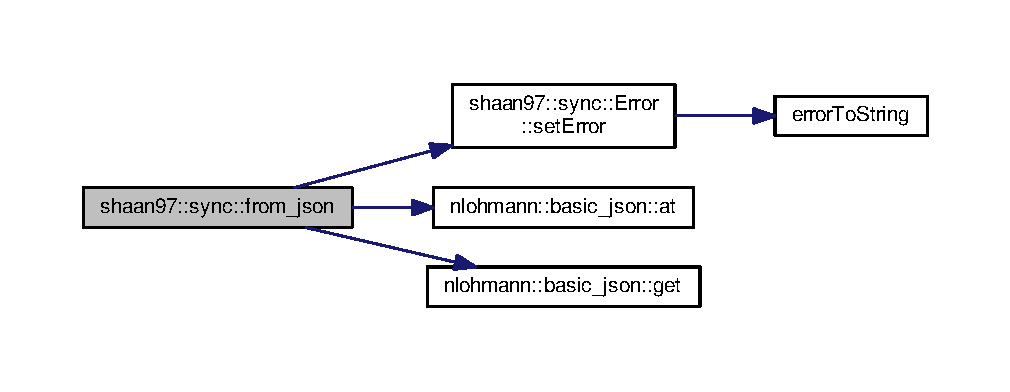
\includegraphics[width=350pt]{namespaceshaan97_1_1sync_a9e374973ba3aed17d32efd550318c94c_cgraph}
\end{center}
\end{figure}
\mbox{\Hypertarget{namespaceshaan97_1_1sync_a734625a59747d9c85857e245a8975bb9}\label{namespaceshaan97_1_1sync_a734625a59747d9c85857e245a8975bb9}} 
\index{shaan97\+::sync@{shaan97\+::sync}!operator$<$$<$@{operator$<$$<$}}
\index{operator$<$$<$@{operator$<$$<$}!shaan97\+::sync@{shaan97\+::sync}}
\subsubsection{\texorpdfstring{operator$<$$<$()}{operator<<()}}
{\footnotesize\ttfamily std\+::ostream \& shaan97\+::sync\+::operator$<$$<$ (\begin{DoxyParamCaption}\item[{std\+::ostream \&}]{out,  }\item[{const \hyperlink{classshaan97_1_1sync_1_1_error}{Error} \&}]{e }\end{DoxyParamCaption})}

\mbox{\Hypertarget{namespaceshaan97_1_1sync_a6ccb9e98c182a3bac3ee37ad64f76bbc}\label{namespaceshaan97_1_1sync_a6ccb9e98c182a3bac3ee37ad64f76bbc}} 
\index{shaan97\+::sync@{shaan97\+::sync}!to\+\_\+json@{to\+\_\+json}}
\index{to\+\_\+json@{to\+\_\+json}!shaan97\+::sync@{shaan97\+::sync}}
\subsubsection{\texorpdfstring{to\+\_\+json()}{to\_json()}}
{\footnotesize\ttfamily void shaan97\+::sync\+::to\+\_\+json (\begin{DoxyParamCaption}\item[{\hyperlink{namespacenlohmann_a2bfd99e845a2e5cd90aeaf1b1431f474}{nlohmann\+::json} \&}]{j,  }\item[{const \hyperlink{classshaan97_1_1sync_1_1_error}{Error} \&}]{e }\end{DoxyParamCaption})}

Converts from {\ttfamily \hyperlink{classshaan97_1_1sync_1_1_error}{Error}} to a {\ttfamily \hyperlink{namespacenlohmann_a2bfd99e845a2e5cd90aeaf1b1431f474}{nlohmann\+::json}} object Here is the call graph for this function\+:\nopagebreak
\begin{figure}[H]
\begin{center}
\leavevmode
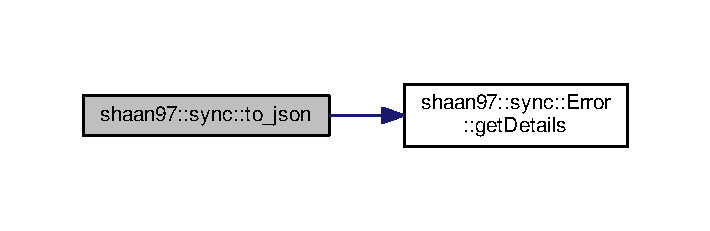
\includegraphics[width=341pt]{namespaceshaan97_1_1sync_a6ccb9e98c182a3bac3ee37ad64f76bbc_cgraph}
\end{center}
\end{figure}

\chapter{Class Documentation}
\hypertarget{structnlohmann_1_1adl__serializer}{}\section{nlohmann\+:\+:adl\+\_\+serializer$<$ typename, typename $>$ Struct Template Reference}
\label{structnlohmann_1_1adl__serializer}\index{nlohmann\+::adl\+\_\+serializer$<$ typename, typename $>$@{nlohmann\+::adl\+\_\+serializer$<$ typename, typename $>$}}


default J\+S\+O\+N\+Serializer template argument  




{\ttfamily \#include $<$json.\+hpp$>$}

\subsection*{Static Public Member Functions}
\begin{DoxyCompactItemize}
\item 
{\footnotesize template$<$typename Basic\+Json\+Type , typename Value\+Type $>$ }\\static void \hyperlink{structnlohmann_1_1adl__serializer_ab39cad07c1a2bf4414d6cae5215b4e7a}{from\+\_\+json} (Basic\+Json\+Type \&\&j, Value\+Type \&val) noexcept(noexcept(\+::nlohmann\+::from\+\_\+json(std\+::forward$<$ Basic\+Json\+Type $>$(j), val)))
\begin{DoxyCompactList}\small\item\em convert a J\+S\+ON value to any value type \end{DoxyCompactList}\item 
{\footnotesize template$<$typename Basic\+Json\+Type , typename Value\+Type $>$ }\\static void \hyperlink{structnlohmann_1_1adl__serializer_adf8cd96afe6ab243b67392dfe35ace89}{to\+\_\+json} (Basic\+Json\+Type \&j, Value\+Type \&\&val) noexcept(noexcept(\+::nlohmann\+::to\+\_\+json(j, std\+::forward$<$ Value\+Type $>$(val))))
\begin{DoxyCompactList}\small\item\em convert any value type to a J\+S\+ON value \end{DoxyCompactList}\end{DoxyCompactItemize}


\subsection{Detailed Description}
\subsubsection*{template$<$typename = void, typename = void$>$\newline
struct nlohmann\+::adl\+\_\+serializer$<$ typename, typename $>$}

default J\+S\+O\+N\+Serializer template argument 

This serializer ignores the template arguments and uses A\+DL (\href{http://en.cppreference.com/w/cpp/language/adl}{\tt argument-\/dependent lookup}) for serialization. 

\subsection{Member Function Documentation}
\mbox{\Hypertarget{structnlohmann_1_1adl__serializer_ab39cad07c1a2bf4414d6cae5215b4e7a}\label{structnlohmann_1_1adl__serializer_ab39cad07c1a2bf4414d6cae5215b4e7a}} 
\index{nlohmann\+::adl\+\_\+serializer@{nlohmann\+::adl\+\_\+serializer}!from\+\_\+json@{from\+\_\+json}}
\index{from\+\_\+json@{from\+\_\+json}!nlohmann\+::adl\+\_\+serializer@{nlohmann\+::adl\+\_\+serializer}}
\subsubsection{\texorpdfstring{from\+\_\+json()}{from\_json()}}
{\footnotesize\ttfamily template$<$typename  = void, typename  = void$>$ \\
template$<$typename Basic\+Json\+Type , typename Value\+Type $>$ \\
static void \hyperlink{structnlohmann_1_1adl__serializer}{nlohmann\+::adl\+\_\+serializer}$<$ typename, typename $>$\+::from\+\_\+json (\begin{DoxyParamCaption}\item[{Basic\+Json\+Type \&\&}]{j,  }\item[{Value\+Type \&}]{val }\end{DoxyParamCaption})\hspace{0.3cm}{\ttfamily [inline]}, {\ttfamily [static]}, {\ttfamily [noexcept]}}



convert a J\+S\+ON value to any value type 

This function is usually called by the {\ttfamily get()} function of the \hyperlink{classnlohmann_1_1basic__json}{basic\+\_\+json} class (either explicit or via conversion operators).


\begin{DoxyParams}[1]{Parameters}
\mbox{\tt in}  & {\em j} & J\+S\+ON value to read from \\
\hline
\mbox{\tt in,out}  & {\em val} & value to write to \\
\hline
\end{DoxyParams}
Here is the call graph for this function\+:\nopagebreak
\begin{figure}[H]
\begin{center}
\leavevmode
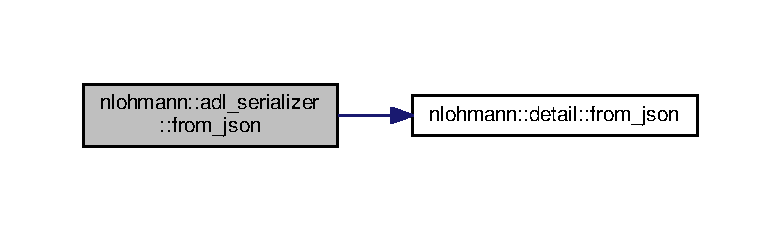
\includegraphics[width=350pt]{structnlohmann_1_1adl__serializer_ab39cad07c1a2bf4414d6cae5215b4e7a_cgraph}
\end{center}
\end{figure}
\mbox{\Hypertarget{structnlohmann_1_1adl__serializer_adf8cd96afe6ab243b67392dfe35ace89}\label{structnlohmann_1_1adl__serializer_adf8cd96afe6ab243b67392dfe35ace89}} 
\index{nlohmann\+::adl\+\_\+serializer@{nlohmann\+::adl\+\_\+serializer}!to\+\_\+json@{to\+\_\+json}}
\index{to\+\_\+json@{to\+\_\+json}!nlohmann\+::adl\+\_\+serializer@{nlohmann\+::adl\+\_\+serializer}}
\subsubsection{\texorpdfstring{to\+\_\+json()}{to\_json()}}
{\footnotesize\ttfamily template$<$typename  = void, typename  = void$>$ \\
template$<$typename Basic\+Json\+Type , typename Value\+Type $>$ \\
static void \hyperlink{structnlohmann_1_1adl__serializer}{nlohmann\+::adl\+\_\+serializer}$<$ typename, typename $>$\+::to\+\_\+json (\begin{DoxyParamCaption}\item[{Basic\+Json\+Type \&}]{j,  }\item[{Value\+Type \&\&}]{val }\end{DoxyParamCaption})\hspace{0.3cm}{\ttfamily [inline]}, {\ttfamily [static]}, {\ttfamily [noexcept]}}



convert any value type to a J\+S\+ON value 

This function is usually called by the constructors of the \hyperlink{classnlohmann_1_1basic__json}{basic\+\_\+json} class.


\begin{DoxyParams}[1]{Parameters}
\mbox{\tt in,out}  & {\em j} & J\+S\+ON value to write to \\
\hline
\mbox{\tt in}  & {\em val} & value to read from \\
\hline
\end{DoxyParams}
Here is the call graph for this function\+:\nopagebreak
\begin{figure}[H]
\begin{center}
\leavevmode
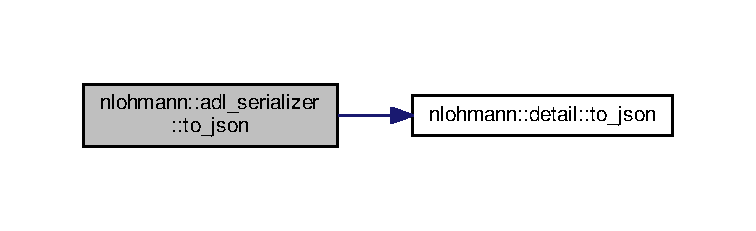
\includegraphics[width=350pt]{structnlohmann_1_1adl__serializer_adf8cd96afe6ab243b67392dfe35ace89_cgraph}
\end{center}
\end{figure}


The documentation for this struct was generated from the following file\+:\begin{DoxyCompactItemize}
\item 
/home/shaan/\+Desktop/\+Computer Science/\+Sync/inc/\hyperlink{json_8hpp}{json.\+hpp}\end{DoxyCompactItemize}

\hypertarget{classnlohmann_1_1basic__json}{}\section{nlohmann\+:\+:basic\+\_\+json$<$ Object\+Type, Array\+Type, String\+Type, Boolean\+Type, Number\+Integer\+Type, Number\+Unsigned\+Type, Number\+Float\+Type, Allocator\+Type, J\+S\+O\+N\+Serializer $>$ Class Template Reference}
\label{classnlohmann_1_1basic__json}\index{nlohmann\+::basic\+\_\+json$<$ Object\+Type, Array\+Type, String\+Type, Boolean\+Type, Number\+Integer\+Type, Number\+Unsigned\+Type, Number\+Float\+Type, Allocator\+Type, J\+S\+O\+N\+Serializer $>$@{nlohmann\+::basic\+\_\+json$<$ Object\+Type, Array\+Type, String\+Type, Boolean\+Type, Number\+Integer\+Type, Number\+Unsigned\+Type, Number\+Float\+Type, Allocator\+Type, J\+S\+O\+N\+Serializer $>$}}


a class to store J\+S\+ON values  




{\ttfamily \#include $<$json.\+hpp$>$}



Collaboration diagram for nlohmann\+:\+:basic\+\_\+json$<$ Object\+Type, Array\+Type, String\+Type, Boolean\+Type, Number\+Integer\+Type, Number\+Unsigned\+Type, Number\+Float\+Type, Allocator\+Type, J\+S\+O\+N\+Serializer $>$\+:\nopagebreak
\begin{figure}[H]
\begin{center}
\leavevmode
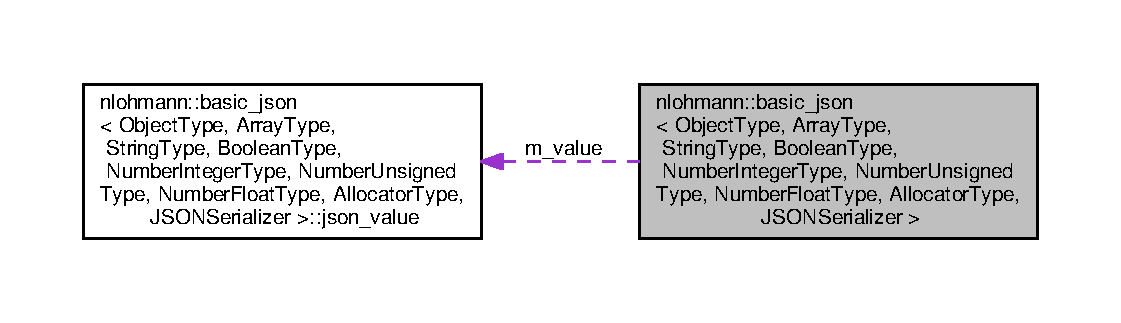
\includegraphics[width=350pt]{classnlohmann_1_1basic__json__coll__graph}
\end{center}
\end{figure}
\subsection*{Classes}
\begin{DoxyCompactItemize}
\item 
struct \hyperlink{structnlohmann_1_1basic__json_1_1internal__iterator}{internal\+\_\+iterator}
\begin{DoxyCompactList}\small\item\em an iterator value \end{DoxyCompactList}\item 
class \hyperlink{classnlohmann_1_1basic__json_1_1iter__impl}{iter\+\_\+impl}
\begin{DoxyCompactList}\small\item\em a template for a random access iterator for the \hyperlink{classnlohmann_1_1basic__json}{basic\+\_\+json} class \end{DoxyCompactList}\item 
class \hyperlink{classnlohmann_1_1basic__json_1_1iteration__proxy}{iteration\+\_\+proxy}
\begin{DoxyCompactList}\small\item\em proxy class for the iterator\+\_\+wrapper functions \end{DoxyCompactList}\item 
class \hyperlink{classnlohmann_1_1basic__json_1_1json__pointer}{json\+\_\+pointer}
\begin{DoxyCompactList}\small\item\em J\+S\+ON Pointer. \end{DoxyCompactList}\item 
class \hyperlink{classnlohmann_1_1basic__json_1_1json__reverse__iterator}{json\+\_\+reverse\+\_\+iterator}
\begin{DoxyCompactList}\small\item\em a template for a reverse iterator class \end{DoxyCompactList}\item 
union \hyperlink{unionnlohmann_1_1basic__json_1_1json__value}{json\+\_\+value}
\begin{DoxyCompactList}\small\item\em a J\+S\+ON value \end{DoxyCompactList}\item 
class \hyperlink{classnlohmann_1_1basic__json_1_1lexer}{lexer}
\begin{DoxyCompactList}\small\item\em lexical analysis \end{DoxyCompactList}\item 
struct \hyperlink{structnlohmann_1_1basic__json_1_1numtostr}{numtostr}
\begin{DoxyCompactList}\small\item\em locale-\/independent serialization for built-\/in arithmetic types \end{DoxyCompactList}\item 
class \hyperlink{classnlohmann_1_1basic__json_1_1parser}{parser}
\begin{DoxyCompactList}\small\item\em syntax analysis \end{DoxyCompactList}\item 
class \hyperlink{classnlohmann_1_1basic__json_1_1primitive__iterator__t}{primitive\+\_\+iterator\+\_\+t}
\begin{DoxyCompactList}\small\item\em an iterator for primitive J\+S\+ON types \end{DoxyCompactList}\end{DoxyCompactItemize}
\subsection*{Public Types}
\begin{DoxyCompactItemize}
\item 
enum \hyperlink{classnlohmann_1_1basic__json_aea1c863b719b4ca5b77188c171bbfafe}{parse\+\_\+event\+\_\+t} \+: uint8\+\_\+t \{ \newline
\hyperlink{classnlohmann_1_1basic__json_aea1c863b719b4ca5b77188c171bbfafeae73f17027cb0acbb537f29d0a6944b26}{parse\+\_\+event\+\_\+t\+::object\+\_\+start}, 
\hyperlink{classnlohmann_1_1basic__json_aea1c863b719b4ca5b77188c171bbfafeaf63e2a2468a37aa4f394fcc3bcb8249c}{parse\+\_\+event\+\_\+t\+::object\+\_\+end}, 
\hyperlink{classnlohmann_1_1basic__json_aea1c863b719b4ca5b77188c171bbfafeaa4388a3d92419edbb1c6efd4d52461f3}{parse\+\_\+event\+\_\+t\+::array\+\_\+start}, 
\hyperlink{classnlohmann_1_1basic__json_aea1c863b719b4ca5b77188c171bbfafea49642fb732aa2e112188fba1f9d3ef7f}{parse\+\_\+event\+\_\+t\+::array\+\_\+end}, 
\newline
\hyperlink{classnlohmann_1_1basic__json_aea1c863b719b4ca5b77188c171bbfafea3c6e0b8a9c15224a8228b9a98ca1531d}{parse\+\_\+event\+\_\+t\+::key}, 
\hyperlink{classnlohmann_1_1basic__json_aea1c863b719b4ca5b77188c171bbfafea2063c1608d6e0baf80249c42e2be5804}{parse\+\_\+event\+\_\+t\+::value}
 \}\begin{DoxyCompactList}\small\item\em J\+S\+ON callback events. \end{DoxyCompactList}
\item 
using \hyperlink{classnlohmann_1_1basic__json_ae8cbef097f7da18a781fc86587de6b90}{value\+\_\+t} = \hyperlink{namespacenlohmann_1_1detail_a90aa5ef615aa8305e9ea20d8a947980f}{detail\+::value\+\_\+t}
\item 
{\footnotesize template$<$typename T , typename S\+F\+I\+N\+AE $>$ }\\using \hyperlink{classnlohmann_1_1basic__json_a7768841baaaa7a21098a401c932efaff}{json\+\_\+serializer} = J\+S\+O\+N\+Serializer$<$ T, S\+F\+I\+N\+AE $>$
\item 
using \hyperlink{classnlohmann_1_1basic__json_aecae491e175f8767c550ae3c59e180e3}{parser\+\_\+callback\+\_\+t} = std\+::function$<$ bool(int depth, \hyperlink{classnlohmann_1_1basic__json_aea1c863b719b4ca5b77188c171bbfafe}{parse\+\_\+event\+\_\+t} event, \hyperlink{classnlohmann_1_1basic__json}{basic\+\_\+json} \&parsed)$>$
\begin{DoxyCompactList}\small\item\em per-\/element parser callback type \end{DoxyCompactList}\end{DoxyCompactItemize}
\subsection*{Public Member Functions}
\begin{DoxyCompactItemize}
\item 
std\+::string \hyperlink{classnlohmann_1_1basic__json_a6b75862bdb4d26650616cf9821430755}{type\+\_\+name} () const
\begin{DoxyCompactList}\small\item\em return the type as string \end{DoxyCompactList}\end{DoxyCompactItemize}
\subsection*{Static Public Member Functions}
\begin{DoxyCompactItemize}
\item 
static \hyperlink{classnlohmann_1_1basic__json_a86ce930490cf7773b26f5ef49c04a350}{allocator\+\_\+type} \hyperlink{classnlohmann_1_1basic__json_af4ac14224fbdd29d3547fcb11bb55c8f}{get\+\_\+allocator} ()
\begin{DoxyCompactList}\small\item\em returns the allocator associated with the container \end{DoxyCompactList}\item 
static \hyperlink{classnlohmann_1_1basic__json}{basic\+\_\+json} \hyperlink{classnlohmann_1_1basic__json_aef6d0eeccee7c5c7e1317c2ea1607fab}{meta} ()
\begin{DoxyCompactList}\small\item\em returns version information on the library \end{DoxyCompactList}\end{DoxyCompactItemize}
\subsection*{Private Types}
\begin{DoxyCompactItemize}
\item 
using \hyperlink{classnlohmann_1_1basic__json_afc4033f5af721feb287b0676723a145f}{basic\+\_\+json\+\_\+t} = \hyperlink{classnlohmann_1_1basic__json}{basic\+\_\+json}$<$ Object\+Type, Array\+Type, String\+Type, Boolean\+Type, Number\+Integer\+Type, Number\+Unsigned\+Type, Number\+Float\+Type, Allocator\+Type, J\+S\+O\+N\+Serializer $>$
\begin{DoxyCompactList}\small\item\em workaround type for M\+S\+VC \end{DoxyCompactList}\end{DoxyCompactItemize}
\subsection*{Private Member Functions}
\begin{DoxyCompactItemize}
\item 
void \hyperlink{classnlohmann_1_1basic__json_a13453ed62f2b771dea9923119beb4f7c}{assert\+\_\+invariant} () const
\begin{DoxyCompactList}\small\item\em checks the class invariants \end{DoxyCompactList}\item 
\hyperlink{classnlohmann_1_1basic__json_a4c919102a9b4fe0d588af64801436082}{boolean\+\_\+t} \hyperlink{classnlohmann_1_1basic__json_ac686d87a2261f85f1df97035b14a6e3a}{get\+\_\+impl} (\hyperlink{classnlohmann_1_1basic__json_a4c919102a9b4fe0d588af64801436082}{boolean\+\_\+t} $\ast$) const
\begin{DoxyCompactList}\small\item\em get a boolean (explicit) \end{DoxyCompactList}\item 
\hyperlink{classnlohmann_1_1basic__json_aa1eb13d5aa86f80cbee6c58e90fbaf49}{object\+\_\+t} $\ast$ \hyperlink{classnlohmann_1_1basic__json_a58b65f595883fb93333423ec5e3bafee}{get\+\_\+impl\+\_\+ptr} (\hyperlink{classnlohmann_1_1basic__json_aa1eb13d5aa86f80cbee6c58e90fbaf49}{object\+\_\+t} $\ast$) noexcept
\begin{DoxyCompactList}\small\item\em get a pointer to the value (object) \end{DoxyCompactList}\item 
constexpr const \hyperlink{classnlohmann_1_1basic__json_aa1eb13d5aa86f80cbee6c58e90fbaf49}{object\+\_\+t} $\ast$ \hyperlink{classnlohmann_1_1basic__json_aff66aa31ef8603d799433b26fe7535c9}{get\+\_\+impl\+\_\+ptr} (const \hyperlink{classnlohmann_1_1basic__json_aa1eb13d5aa86f80cbee6c58e90fbaf49}{object\+\_\+t} $\ast$) const noexcept
\begin{DoxyCompactList}\small\item\em get a pointer to the value (object) \end{DoxyCompactList}\item 
\hyperlink{classnlohmann_1_1basic__json_ae095578e03df97c5b3991787f1056374}{array\+\_\+t} $\ast$ \hyperlink{classnlohmann_1_1basic__json_a0a9c36d4d94ef5d611c0204bc7e4d37f}{get\+\_\+impl\+\_\+ptr} (\hyperlink{classnlohmann_1_1basic__json_ae095578e03df97c5b3991787f1056374}{array\+\_\+t} $\ast$) noexcept
\begin{DoxyCompactList}\small\item\em get a pointer to the value (array) \end{DoxyCompactList}\item 
constexpr const \hyperlink{classnlohmann_1_1basic__json_ae095578e03df97c5b3991787f1056374}{array\+\_\+t} $\ast$ \hyperlink{classnlohmann_1_1basic__json_abefb50a81c9b91106d9ecadfcd1ee2b5}{get\+\_\+impl\+\_\+ptr} (const \hyperlink{classnlohmann_1_1basic__json_ae095578e03df97c5b3991787f1056374}{array\+\_\+t} $\ast$) const noexcept
\begin{DoxyCompactList}\small\item\em get a pointer to the value (array) \end{DoxyCompactList}\item 
\hyperlink{classnlohmann_1_1basic__json_a61f8566a1a85a424c7266fb531dca005}{string\+\_\+t} $\ast$ \hyperlink{classnlohmann_1_1basic__json_a955d7098e5b43ee0dd8cce5f707eeb5c}{get\+\_\+impl\+\_\+ptr} (\hyperlink{classnlohmann_1_1basic__json_a61f8566a1a85a424c7266fb531dca005}{string\+\_\+t} $\ast$) noexcept
\begin{DoxyCompactList}\small\item\em get a pointer to the value (string) \end{DoxyCompactList}\item 
constexpr const \hyperlink{classnlohmann_1_1basic__json_a61f8566a1a85a424c7266fb531dca005}{string\+\_\+t} $\ast$ \hyperlink{classnlohmann_1_1basic__json_a0c0b516e06d10dced993934ba5139cc0}{get\+\_\+impl\+\_\+ptr} (const \hyperlink{classnlohmann_1_1basic__json_a61f8566a1a85a424c7266fb531dca005}{string\+\_\+t} $\ast$) const noexcept
\begin{DoxyCompactList}\small\item\em get a pointer to the value (string) \end{DoxyCompactList}\item 
\hyperlink{classnlohmann_1_1basic__json_a4c919102a9b4fe0d588af64801436082}{boolean\+\_\+t} $\ast$ \hyperlink{classnlohmann_1_1basic__json_ab1678fb6723faf020a15300c4f6b98f5}{get\+\_\+impl\+\_\+ptr} (\hyperlink{classnlohmann_1_1basic__json_a4c919102a9b4fe0d588af64801436082}{boolean\+\_\+t} $\ast$) noexcept
\begin{DoxyCompactList}\small\item\em get a pointer to the value (boolean) \end{DoxyCompactList}\item 
constexpr const \hyperlink{classnlohmann_1_1basic__json_a4c919102a9b4fe0d588af64801436082}{boolean\+\_\+t} $\ast$ \hyperlink{classnlohmann_1_1basic__json_ae068eee75c0a814e19208bae641f866c}{get\+\_\+impl\+\_\+ptr} (const \hyperlink{classnlohmann_1_1basic__json_a4c919102a9b4fe0d588af64801436082}{boolean\+\_\+t} $\ast$) const noexcept
\begin{DoxyCompactList}\small\item\em get a pointer to the value (boolean) \end{DoxyCompactList}\item 
\hyperlink{classnlohmann_1_1basic__json_a98e611d67b7bd75307de99c9358ab2dc}{number\+\_\+integer\+\_\+t} $\ast$ \hyperlink{classnlohmann_1_1basic__json_a32a4c3ccdd09b663614adce1834a0a50}{get\+\_\+impl\+\_\+ptr} (\hyperlink{classnlohmann_1_1basic__json_a98e611d67b7bd75307de99c9358ab2dc}{number\+\_\+integer\+\_\+t} $\ast$) noexcept
\begin{DoxyCompactList}\small\item\em get a pointer to the value (integer number) \end{DoxyCompactList}\item 
constexpr const \hyperlink{classnlohmann_1_1basic__json_a98e611d67b7bd75307de99c9358ab2dc}{number\+\_\+integer\+\_\+t} $\ast$ \hyperlink{classnlohmann_1_1basic__json_a0a01103792cc54e9c8236361e5f7ed90}{get\+\_\+impl\+\_\+ptr} (const \hyperlink{classnlohmann_1_1basic__json_a98e611d67b7bd75307de99c9358ab2dc}{number\+\_\+integer\+\_\+t} $\ast$) const noexcept
\begin{DoxyCompactList}\small\item\em get a pointer to the value (integer number) \end{DoxyCompactList}\item 
\hyperlink{classnlohmann_1_1basic__json_ab906e29b5d83ac162e823ada2156b989}{number\+\_\+unsigned\+\_\+t} $\ast$ \hyperlink{classnlohmann_1_1basic__json_aa9aaed6b92909b263e04b5d25eba8d67}{get\+\_\+impl\+\_\+ptr} (\hyperlink{classnlohmann_1_1basic__json_ab906e29b5d83ac162e823ada2156b989}{number\+\_\+unsigned\+\_\+t} $\ast$) noexcept
\begin{DoxyCompactList}\small\item\em get a pointer to the value (unsigned number) \end{DoxyCompactList}\item 
constexpr const \hyperlink{classnlohmann_1_1basic__json_ab906e29b5d83ac162e823ada2156b989}{number\+\_\+unsigned\+\_\+t} $\ast$ \hyperlink{classnlohmann_1_1basic__json_a52d0c7f354c6155221540baef5b98d0a}{get\+\_\+impl\+\_\+ptr} (const \hyperlink{classnlohmann_1_1basic__json_ab906e29b5d83ac162e823ada2156b989}{number\+\_\+unsigned\+\_\+t} $\ast$) const noexcept
\begin{DoxyCompactList}\small\item\em get a pointer to the value (unsigned number) \end{DoxyCompactList}\item 
\hyperlink{classnlohmann_1_1basic__json_a88d6103cb3620410b35200ee8e313d97}{number\+\_\+float\+\_\+t} $\ast$ \hyperlink{classnlohmann_1_1basic__json_a01e81365c2c6897b39b793530e02aca5}{get\+\_\+impl\+\_\+ptr} (\hyperlink{classnlohmann_1_1basic__json_a88d6103cb3620410b35200ee8e313d97}{number\+\_\+float\+\_\+t} $\ast$) noexcept
\begin{DoxyCompactList}\small\item\em get a pointer to the value (floating-\/point number) \end{DoxyCompactList}\item 
constexpr const \hyperlink{classnlohmann_1_1basic__json_a88d6103cb3620410b35200ee8e313d97}{number\+\_\+float\+\_\+t} $\ast$ \hyperlink{classnlohmann_1_1basic__json_abbec23daef5fbb5b8bff6a481e5a7160}{get\+\_\+impl\+\_\+ptr} (const \hyperlink{classnlohmann_1_1basic__json_a88d6103cb3620410b35200ee8e313d97}{number\+\_\+float\+\_\+t} $\ast$) const noexcept
\begin{DoxyCompactList}\small\item\em get a pointer to the value (floating-\/point number) \end{DoxyCompactList}\item 
void \hyperlink{classnlohmann_1_1basic__json_ade04010df46f1f247623b85191976239}{dump} (std\+::ostream \&o, const bool pretty\+\_\+print, const unsigned int indent\+\_\+step, const unsigned int current\+\_\+indent=0) const
\begin{DoxyCompactList}\small\item\em internal implementation of the serialization function \end{DoxyCompactList}\end{DoxyCompactItemize}
\subsection*{Static Private Member Functions}
\begin{DoxyCompactItemize}
\item 
{\footnotesize template$<$typename T , typename... Args$>$ }\\static T $\ast$ \hyperlink{classnlohmann_1_1basic__json_a81100399cf3e2be457937be7db3f5729}{create} (Args \&\&... args)
\begin{DoxyCompactList}\small\item\em helper for exception-\/safe object creation \end{DoxyCompactList}\item 
{\footnotesize template$<$typename Reference\+Type , typename This\+Type $>$ }\\static Reference\+Type \hyperlink{classnlohmann_1_1basic__json_a040a5feb1eb48da9134924217b25bcf6}{get\+\_\+ref\+\_\+impl} (This\+Type \&obj)
\begin{DoxyCompactList}\small\item\em helper function to implement \hyperlink{classnlohmann_1_1basic__json_afbd800010b67619463c0fce6e74f7878}{get\+\_\+ref()} \end{DoxyCompactList}\item 
static std\+::size\+\_\+t \hyperlink{classnlohmann_1_1basic__json_ab47d5e44bf890f791a597b1f55afb38e}{extra\+\_\+space} (const \hyperlink{classnlohmann_1_1basic__json_a61f8566a1a85a424c7266fb531dca005}{string\+\_\+t} \&s) noexcept
\begin{DoxyCompactList}\small\item\em calculates the extra space to escape a J\+S\+ON string \end{DoxyCompactList}\item 
static \hyperlink{classnlohmann_1_1basic__json_a61f8566a1a85a424c7266fb531dca005}{string\+\_\+t} \hyperlink{classnlohmann_1_1basic__json_af6e1e06b6c274734ccb7de1ef770a915}{escape\+\_\+string} (const \hyperlink{classnlohmann_1_1basic__json_a61f8566a1a85a424c7266fb531dca005}{string\+\_\+t} \&s)
\begin{DoxyCompactList}\small\item\em escape a string \end{DoxyCompactList}\end{DoxyCompactItemize}
\subsection*{Private Attributes}
\begin{DoxyCompactItemize}
\item 
\hyperlink{namespacenlohmann_1_1detail_a90aa5ef615aa8305e9ea20d8a947980f}{value\+\_\+t} \hyperlink{classnlohmann_1_1basic__json_a91990b60d7d4d67968a2c1db677536e7}{m\+\_\+type} = value\+\_\+t\+::null
\begin{DoxyCompactList}\small\item\em the type of the current element \end{DoxyCompactList}\item 
\hyperlink{unionnlohmann_1_1basic__json_1_1json__value}{json\+\_\+value} \hyperlink{classnlohmann_1_1basic__json_aeb0814f76966f99290cb29e127c90a77}{m\+\_\+value} = \{\}
\begin{DoxyCompactList}\small\item\em the value of the current element \end{DoxyCompactList}\end{DoxyCompactItemize}
\subsection*{Friends}
\begin{DoxyCompactItemize}
\item 
{\footnotesize template$<$detail\+::value\+\_\+t $>$ }\\struct \hyperlink{classnlohmann_1_1basic__json_a6275ed57bae6866cdf5db5370a7ad47c}{detail\+::external\+\_\+constructor}
\end{DoxyCompactItemize}
\subsection*{container types}
\label{_amgrp6618fa684bc6d5a05e2c88bfff1c0d66}%
The canonic container types to use \hyperlink{classnlohmann_1_1basic__json}{basic\+\_\+json} like any other S\+TL container. \begin{DoxyCompactItemize}
\item 
using \hyperlink{classnlohmann_1_1basic__json_a2b3297873b70c080837e8eedc4fec32f}{value\+\_\+type} = \hyperlink{classnlohmann_1_1basic__json}{basic\+\_\+json}
\begin{DoxyCompactList}\small\item\em the type of elements in a \hyperlink{classnlohmann_1_1basic__json}{basic\+\_\+json} container \end{DoxyCompactList}\item 
using \hyperlink{classnlohmann_1_1basic__json_ac6a5eddd156c776ac75ff54cfe54a5bc}{reference} = \hyperlink{classnlohmann_1_1basic__json_a2b3297873b70c080837e8eedc4fec32f}{value\+\_\+type} \&
\begin{DoxyCompactList}\small\item\em the type of an element reference \end{DoxyCompactList}\item 
using \hyperlink{classnlohmann_1_1basic__json_a4057c5425f4faacfe39a8046871786ca}{const\+\_\+reference} = const \hyperlink{classnlohmann_1_1basic__json_a2b3297873b70c080837e8eedc4fec32f}{value\+\_\+type} \&
\begin{DoxyCompactList}\small\item\em the type of an element const reference \end{DoxyCompactList}\item 
using \hyperlink{classnlohmann_1_1basic__json_afe7c1303357e19cea9527af4e9a31d8f}{difference\+\_\+type} = std\+::ptrdiff\+\_\+t
\begin{DoxyCompactList}\small\item\em a type to represent differences between iterators \end{DoxyCompactList}\item 
using \hyperlink{classnlohmann_1_1basic__json_a39f2cd0b58106097e0e67bf185cc519b}{size\+\_\+type} = std\+::size\+\_\+t
\begin{DoxyCompactList}\small\item\em a type to represent container sizes \end{DoxyCompactList}\item 
using \hyperlink{classnlohmann_1_1basic__json_a86ce930490cf7773b26f5ef49c04a350}{allocator\+\_\+type} = Allocator\+Type$<$ \hyperlink{classnlohmann_1_1basic__json}{basic\+\_\+json} $>$
\begin{DoxyCompactList}\small\item\em the allocator type \end{DoxyCompactList}\item 
using \hyperlink{classnlohmann_1_1basic__json_aefee1f777198c68724bd127e0c8abbe4}{pointer} = typename std\+::allocator\+\_\+traits$<$ \hyperlink{classnlohmann_1_1basic__json_a86ce930490cf7773b26f5ef49c04a350}{allocator\+\_\+type} $>$\+::\hyperlink{classnlohmann_1_1basic__json_aefee1f777198c68724bd127e0c8abbe4}{pointer}
\begin{DoxyCompactList}\small\item\em the type of an element pointer \end{DoxyCompactList}\item 
using \hyperlink{classnlohmann_1_1basic__json_aff3d5cd2a75612364b888d8693231b58}{const\+\_\+pointer} = typename std\+::allocator\+\_\+traits$<$ \hyperlink{classnlohmann_1_1basic__json_a86ce930490cf7773b26f5ef49c04a350}{allocator\+\_\+type} $>$\+::\hyperlink{classnlohmann_1_1basic__json_aff3d5cd2a75612364b888d8693231b58}{const\+\_\+pointer}
\begin{DoxyCompactList}\small\item\em the type of an element const pointer \end{DoxyCompactList}\item 
using \hyperlink{classnlohmann_1_1basic__json_a099316232c76c034030a38faa6e34dca}{iterator} = \hyperlink{classnlohmann_1_1basic__json_1_1iter__impl}{iter\+\_\+impl}$<$ \hyperlink{classnlohmann_1_1basic__json}{basic\+\_\+json} $>$
\begin{DoxyCompactList}\small\item\em an iterator for a \hyperlink{classnlohmann_1_1basic__json}{basic\+\_\+json} container \end{DoxyCompactList}\item 
using \hyperlink{classnlohmann_1_1basic__json_a41a70cf9993951836d129bb1c2b3126a}{const\+\_\+iterator} = \hyperlink{classnlohmann_1_1basic__json_1_1iter__impl}{iter\+\_\+impl}$<$ const \hyperlink{classnlohmann_1_1basic__json}{basic\+\_\+json} $>$
\begin{DoxyCompactList}\small\item\em a const iterator for a \hyperlink{classnlohmann_1_1basic__json}{basic\+\_\+json} container \end{DoxyCompactList}\item 
using \hyperlink{classnlohmann_1_1basic__json_ac223d5560c2b05a208c88de67376c5f2}{reverse\+\_\+iterator} = \hyperlink{classnlohmann_1_1basic__json_1_1json__reverse__iterator}{json\+\_\+reverse\+\_\+iterator}$<$ typename \hyperlink{classnlohmann_1_1basic__json_a099316232c76c034030a38faa6e34dca}{basic\+\_\+json\+::iterator} $>$
\begin{DoxyCompactList}\small\item\em a reverse iterator for a \hyperlink{classnlohmann_1_1basic__json}{basic\+\_\+json} container \end{DoxyCompactList}\item 
using \hyperlink{classnlohmann_1_1basic__json_a72be3c24bfa24f0993d6c11af03e7404}{const\+\_\+reverse\+\_\+iterator} = \hyperlink{classnlohmann_1_1basic__json_1_1json__reverse__iterator}{json\+\_\+reverse\+\_\+iterator}$<$ typename \hyperlink{classnlohmann_1_1basic__json_a41a70cf9993951836d129bb1c2b3126a}{basic\+\_\+json\+::const\+\_\+iterator} $>$
\begin{DoxyCompactList}\small\item\em a const reverse iterator for a \hyperlink{classnlohmann_1_1basic__json}{basic\+\_\+json} container \end{DoxyCompactList}\end{DoxyCompactItemize}
\subsection*{J\+S\+ON value data types}
\label{_amgrpbddfba6d49869d59bfd397e65b8cba87}%
The data types to store a J\+S\+ON value. These types are derived from the template arguments passed to class \hyperlink{classnlohmann_1_1basic__json}{basic\+\_\+json}. \begin{DoxyCompactItemize}
\item 
using \hyperlink{classnlohmann_1_1basic__json_aa1eb13d5aa86f80cbee6c58e90fbaf49}{object\+\_\+t} = Object\+Type$<$ String\+Type, \hyperlink{classnlohmann_1_1basic__json}{basic\+\_\+json}, std\+::less$<$ String\+Type $>$, Allocator\+Type$<$ std\+::pair$<$ const String\+Type, \hyperlink{classnlohmann_1_1basic__json}{basic\+\_\+json} $>$ $>$$>$
\begin{DoxyCompactList}\small\item\em a type for an object \end{DoxyCompactList}\item 
using \hyperlink{classnlohmann_1_1basic__json_ae095578e03df97c5b3991787f1056374}{array\+\_\+t} = Array\+Type$<$ \hyperlink{classnlohmann_1_1basic__json}{basic\+\_\+json}, Allocator\+Type$<$ \hyperlink{classnlohmann_1_1basic__json}{basic\+\_\+json} $>$ $>$
\begin{DoxyCompactList}\small\item\em a type for an array \end{DoxyCompactList}\item 
using \hyperlink{classnlohmann_1_1basic__json_a61f8566a1a85a424c7266fb531dca005}{string\+\_\+t} = String\+Type
\begin{DoxyCompactList}\small\item\em a type for a string \end{DoxyCompactList}\item 
using \hyperlink{classnlohmann_1_1basic__json_a4c919102a9b4fe0d588af64801436082}{boolean\+\_\+t} = Boolean\+Type
\begin{DoxyCompactList}\small\item\em a type for a boolean \end{DoxyCompactList}\item 
using \hyperlink{classnlohmann_1_1basic__json_a98e611d67b7bd75307de99c9358ab2dc}{number\+\_\+integer\+\_\+t} = Number\+Integer\+Type
\begin{DoxyCompactList}\small\item\em a type for a number (integer) \end{DoxyCompactList}\item 
using \hyperlink{classnlohmann_1_1basic__json_ab906e29b5d83ac162e823ada2156b989}{number\+\_\+unsigned\+\_\+t} = Number\+Unsigned\+Type
\begin{DoxyCompactList}\small\item\em a type for a number (unsigned) \end{DoxyCompactList}\item 
using \hyperlink{classnlohmann_1_1basic__json_a88d6103cb3620410b35200ee8e313d97}{number\+\_\+float\+\_\+t} = Number\+Float\+Type
\begin{DoxyCompactList}\small\item\em a type for a number (floating-\/point) \end{DoxyCompactList}\end{DoxyCompactItemize}
\subsection*{constructors and destructors}
\label{_amgrpd94b4d3d0135946bb7bdf25e48755337}%
Constructors of class \hyperlink{classnlohmann_1_1basic__json}{basic\+\_\+json}, copy/move constructor, copy assignment, static functions creating objects, and the destructor. \begin{DoxyCompactItemize}
\item 
static \hyperlink{classnlohmann_1_1basic__json}{basic\+\_\+json} \hyperlink{classnlohmann_1_1basic__json_a4a4ec75e4d2845d9bcf7a9e5458e4949}{array} (std\+::initializer\+\_\+list$<$ \hyperlink{classnlohmann_1_1basic__json}{basic\+\_\+json} $>$ init=std\+::initializer\+\_\+list$<$ \hyperlink{classnlohmann_1_1basic__json}{basic\+\_\+json} $>$())
\begin{DoxyCompactList}\small\item\em explicitly create an array from an initializer list \end{DoxyCompactList}\item 
static \hyperlink{classnlohmann_1_1basic__json}{basic\+\_\+json} \hyperlink{classnlohmann_1_1basic__json_a9f42ee7d10eee2d5a73fd94ca7f767ca}{object} (std\+::initializer\+\_\+list$<$ \hyperlink{classnlohmann_1_1basic__json}{basic\+\_\+json} $>$ init=std\+::initializer\+\_\+list$<$ \hyperlink{classnlohmann_1_1basic__json}{basic\+\_\+json} $>$())
\begin{DoxyCompactList}\small\item\em explicitly create an object from an initializer list \end{DoxyCompactList}\item 
\hyperlink{classnlohmann_1_1basic__json_a32124a16dc80729d964d9caf607c2bc8}{basic\+\_\+json} (const \hyperlink{namespacenlohmann_1_1detail_a90aa5ef615aa8305e9ea20d8a947980f}{value\+\_\+t} \hyperlink{classnlohmann_1_1basic__json_a2b3297873b70c080837e8eedc4fec32f}{value\+\_\+type})
\begin{DoxyCompactList}\small\item\em create an empty value with a given type \end{DoxyCompactList}\item 
\hyperlink{classnlohmann_1_1basic__json_ae9be9e956bfc4658f35d17c6aa72b063}{basic\+\_\+json} (std\+::nullptr\+\_\+t=nullptr) noexcept
\begin{DoxyCompactList}\small\item\em create a null object \end{DoxyCompactList}\item 
{\footnotesize template$<$typename Compatible\+Type , typename U  = detail\+::uncvref\+\_\+t$<$\+Compatible\+Type$>$, detail\+::enable\+\_\+if\+\_\+t$<$ not std\+::is\+\_\+base\+\_\+of$<$ std\+::istream, U $>$\+::value and not std\+::is\+\_\+same$<$ U, basic\+\_\+json\+\_\+t $>$\+::value and not detail\+::is\+\_\+basic\+\_\+json\+\_\+nested\+\_\+type$<$ basic\+\_\+json\+\_\+t, U $>$\+::value and detail\+::has\+\_\+to\+\_\+json$<$ basic\+\_\+json, U $>$\+::value, int $>$  = 0$>$ }\\\hyperlink{classnlohmann_1_1basic__json_a5a6558bfd1be139a638f91f0e09fc737}{basic\+\_\+json} (Compatible\+Type \&\&val) noexcept(noexcept(J\+S\+O\+N\+Serializer$<$ U $>$\+::\hyperlink{group___serialization_ga213581ca789d5151c699fb4cb30db916}{to\+\_\+json}(std\+::declval$<$ \hyperlink{classnlohmann_1_1basic__json_afc4033f5af721feb287b0676723a145f}{basic\+\_\+json\+\_\+t} \&$>$(), std\+::forward$<$ Compatible\+Type $>$(val))))
\begin{DoxyCompactList}\small\item\em create a J\+S\+ON value \end{DoxyCompactList}\item 
\hyperlink{classnlohmann_1_1basic__json_afbad48316e7cd37366ba3ac5d7e5859e}{basic\+\_\+json} (std\+::initializer\+\_\+list$<$ \hyperlink{classnlohmann_1_1basic__json}{basic\+\_\+json} $>$ init, bool type\+\_\+deduction=true, \hyperlink{namespacenlohmann_1_1detail_a90aa5ef615aa8305e9ea20d8a947980f}{value\+\_\+t} manual\+\_\+type=\hyperlink{namespacenlohmann_1_1detail_a90aa5ef615aa8305e9ea20d8a947980faf1f713c9e000f5d3f280adbd124df4f5}{value\+\_\+t\+::array})
\begin{DoxyCompactList}\small\item\em create a container (array or object) from an initializer list \end{DoxyCompactList}\item 
\hyperlink{classnlohmann_1_1basic__json_ab6816ae5100409254ed0a8bc21c387bb}{basic\+\_\+json} (\hyperlink{classnlohmann_1_1basic__json_a39f2cd0b58106097e0e67bf185cc519b}{size\+\_\+type} cnt, const \hyperlink{classnlohmann_1_1basic__json}{basic\+\_\+json} \&val)
\begin{DoxyCompactList}\small\item\em construct an array with count copies of given value \end{DoxyCompactList}\item 
{\footnotesize template$<$class Input\+IT , typename std\+::enable\+\_\+if$<$ std\+::is\+\_\+same$<$ Input\+I\+T, typename basic\+\_\+json\+\_\+t\+::iterator $>$\+::value or std\+::is\+\_\+same$<$ Input\+I\+T, typename basic\+\_\+json\+\_\+t\+::const\+\_\+iterator $>$\+::value, int $>$\+::type  = 0$>$ }\\\hyperlink{classnlohmann_1_1basic__json_abe197e9f3184487805cfb5bba6fd5938}{basic\+\_\+json} (Input\+IT first, Input\+IT last)
\begin{DoxyCompactList}\small\item\em construct a J\+S\+ON container given an iterator range \end{DoxyCompactList}\item 
\hyperlink{json_8hpp_a584fd8f49cd7f4ecf5baba15b5b53cdd}{J\+S\+O\+N\+\_\+\+D\+E\+P\+R\+E\+C\+A\+T\+ED} \hyperlink{classnlohmann_1_1basic__json_a757e90574a742ae9cc54c97422fb3043}{basic\+\_\+json} (std\+::istream \&i, const \hyperlink{classnlohmann_1_1basic__json_aecae491e175f8767c550ae3c59e180e3}{parser\+\_\+callback\+\_\+t} cb=nullptr)
\begin{DoxyCompactList}\small\item\em construct a J\+S\+ON value given an input stream \end{DoxyCompactList}\item 
\hyperlink{classnlohmann_1_1basic__json_af5de621bcf646c332343f9c1e011126c}{basic\+\_\+json} (const \hyperlink{classnlohmann_1_1basic__json}{basic\+\_\+json} \&other)
\begin{DoxyCompactList}\small\item\em copy constructor \end{DoxyCompactList}\item 
\hyperlink{classnlohmann_1_1basic__json_a9a06d1efd50a00f4889f831f851ce124}{basic\+\_\+json} (\hyperlink{classnlohmann_1_1basic__json}{basic\+\_\+json} \&\&other) noexcept
\begin{DoxyCompactList}\small\item\em move constructor \end{DoxyCompactList}\item 
\hyperlink{classnlohmann_1_1basic__json_ac6a5eddd156c776ac75ff54cfe54a5bc}{reference} \& \hyperlink{classnlohmann_1_1basic__json_aab256df8c5594ec693035822fa1e2904}{operator=} (\hyperlink{classnlohmann_1_1basic__json}{basic\+\_\+json} other) noexcept(std\+::is\+\_\+nothrow\+\_\+move\+\_\+constructible$<$ \hyperlink{namespacenlohmann_1_1detail_a90aa5ef615aa8305e9ea20d8a947980f}{value\+\_\+t} $>$\+::\hyperlink{classnlohmann_1_1basic__json_af9c51328fbe1da75eca750be3009917a}{value} and std\+::is\+\_\+nothrow\+\_\+move\+\_\+assignable$<$ \hyperlink{namespacenlohmann_1_1detail_a90aa5ef615aa8305e9ea20d8a947980f}{value\+\_\+t} $>$\+::\hyperlink{classnlohmann_1_1basic__json_af9c51328fbe1da75eca750be3009917a}{value} and std\+::is\+\_\+nothrow\+\_\+move\+\_\+constructible$<$ \hyperlink{unionnlohmann_1_1basic__json_1_1json__value}{json\+\_\+value} $>$\+::\hyperlink{classnlohmann_1_1basic__json_af9c51328fbe1da75eca750be3009917a}{value} and std\+::is\+\_\+nothrow\+\_\+move\+\_\+assignable$<$ \hyperlink{unionnlohmann_1_1basic__json_1_1json__value}{json\+\_\+value} $>$\+::\hyperlink{classnlohmann_1_1basic__json_af9c51328fbe1da75eca750be3009917a}{value})
\begin{DoxyCompactList}\small\item\em copy assignment \end{DoxyCompactList}\item 
\hyperlink{classnlohmann_1_1basic__json_a42347bbce75ba5571e292a3540af30e0}{$\sim$basic\+\_\+json} ()
\begin{DoxyCompactList}\small\item\em destructor \end{DoxyCompactList}\end{DoxyCompactItemize}
\subsection*{object inspection}
\label{_amgrpbbb01a37b8f261ae5b5799058dcac1a0}%
Functions to inspect the type of a J\+S\+ON value. \begin{DoxyCompactItemize}
\item 
\hyperlink{classnlohmann_1_1basic__json_a61f8566a1a85a424c7266fb531dca005}{string\+\_\+t} \hyperlink{classnlohmann_1_1basic__json_a5319dc1bb9dfe19ce7ff559aaded3422}{dump} (const int indent=-\/1) const
\begin{DoxyCompactList}\small\item\em serialization \end{DoxyCompactList}\item 
constexpr \hyperlink{namespacenlohmann_1_1detail_a90aa5ef615aa8305e9ea20d8a947980f}{value\+\_\+t} \hyperlink{classnlohmann_1_1basic__json_a2b2d781d7f2a4ee41bc0016e931cadf7}{type} () const noexcept
\begin{DoxyCompactList}\small\item\em return the type of the J\+S\+ON value (explicit) \end{DoxyCompactList}\item 
constexpr bool \hyperlink{classnlohmann_1_1basic__json_a6362b88718eb5c6d4fed6a61eed44b95}{is\+\_\+primitive} () const noexcept
\begin{DoxyCompactList}\small\item\em return whether type is primitive \end{DoxyCompactList}\item 
constexpr bool \hyperlink{classnlohmann_1_1basic__json_a9f68a0af820c3ced7f9d17851ce4c22d}{is\+\_\+structured} () const noexcept
\begin{DoxyCompactList}\small\item\em return whether type is structured \end{DoxyCompactList}\item 
constexpr bool \hyperlink{classnlohmann_1_1basic__json_a8faa039ca82427ed29c486ffd00600c3}{is\+\_\+null} () const noexcept
\begin{DoxyCompactList}\small\item\em return whether value is null \end{DoxyCompactList}\item 
constexpr bool \hyperlink{classnlohmann_1_1basic__json_a943e8cb182d0f2365c76d64b42eaa6fd}{is\+\_\+boolean} () const noexcept
\begin{DoxyCompactList}\small\item\em return whether value is a boolean \end{DoxyCompactList}\item 
constexpr bool \hyperlink{classnlohmann_1_1basic__json_a2b9852390abb4b1ef5fac6984e2fc0f3}{is\+\_\+number} () const noexcept
\begin{DoxyCompactList}\small\item\em return whether value is a number \end{DoxyCompactList}\item 
constexpr bool \hyperlink{classnlohmann_1_1basic__json_abac8af76067f1e8fdca9052882c74428}{is\+\_\+number\+\_\+integer} () const noexcept
\begin{DoxyCompactList}\small\item\em return whether value is an integer number \end{DoxyCompactList}\item 
constexpr bool \hyperlink{classnlohmann_1_1basic__json_abc7378cba0613a78b9aad1c8e7044bb0}{is\+\_\+number\+\_\+unsigned} () const noexcept
\begin{DoxyCompactList}\small\item\em return whether value is an unsigned integer number \end{DoxyCompactList}\item 
constexpr bool \hyperlink{classnlohmann_1_1basic__json_a33b4bf898b857c962e798fc7f6e86e70}{is\+\_\+number\+\_\+float} () const noexcept
\begin{DoxyCompactList}\small\item\em return whether value is a floating-\/point number \end{DoxyCompactList}\item 
constexpr bool \hyperlink{classnlohmann_1_1basic__json_af8f511af124e82e4579f444b4175787c}{is\+\_\+object} () const noexcept
\begin{DoxyCompactList}\small\item\em return whether value is an object \end{DoxyCompactList}\item 
constexpr bool \hyperlink{classnlohmann_1_1basic__json_aef9ce5dd2381caee1f8ddcdb5bdd9c65}{is\+\_\+array} () const noexcept
\begin{DoxyCompactList}\small\item\em return whether value is an array \end{DoxyCompactList}\item 
constexpr bool \hyperlink{classnlohmann_1_1basic__json_a69b596a4a6683b362095c9a139637396}{is\+\_\+string} () const noexcept
\begin{DoxyCompactList}\small\item\em return whether value is a string \end{DoxyCompactList}\item 
constexpr bool \hyperlink{classnlohmann_1_1basic__json_aabe623bc8304c2ba92d96d91f390fab4}{is\+\_\+discarded} () const noexcept
\begin{DoxyCompactList}\small\item\em return whether value is discarded \end{DoxyCompactList}\item 
constexpr \hyperlink{classnlohmann_1_1basic__json_a26ef3058e249f82a04f8ec18f7419027}{operator value\+\_\+t} () const noexcept
\begin{DoxyCompactList}\small\item\em return the type of the J\+S\+ON value (implicit) \end{DoxyCompactList}\end{DoxyCompactItemize}
\subsection*{value access}
\label{_amgrpd8f53c9caf18314e5b3f758245606995}%
Direct access to the stored value of a J\+S\+ON value. \begin{DoxyCompactItemize}
\item 
{\footnotesize template$<$typename Basic\+Json\+Type , detail\+::enable\+\_\+if\+\_\+t$<$ std\+::is\+\_\+same$<$ typename std\+::remove\+\_\+const$<$ Basic\+Json\+Type $>$\+::type, basic\+\_\+json\+\_\+t $>$\+::value, int $>$  = 0$>$ }\\\hyperlink{classnlohmann_1_1basic__json}{basic\+\_\+json} \hyperlink{classnlohmann_1_1basic__json_a6b187a22994c12c8cae0dd5ee99dc85e}{get} () const
\begin{DoxyCompactList}\small\item\em get special-\/case overload \end{DoxyCompactList}\item 
{\footnotesize template$<$typename Value\+Type\+CV , typename Value\+Type  = detail\+::uncvref\+\_\+t$<$\+Value\+Type\+C\+V$>$, detail\+::enable\+\_\+if\+\_\+t$<$ not std\+::is\+\_\+same$<$ basic\+\_\+json\+\_\+t, Value\+Type $>$\+::value and detail\+::has\+\_\+from\+\_\+json$<$ basic\+\_\+json\+\_\+t, Value\+Type $>$\+::value and not detail\+::has\+\_\+non\+\_\+default\+\_\+from\+\_\+json$<$ basic\+\_\+json\+\_\+t, Value\+Type $>$\+::value, int $>$  = 0$>$ }\\Value\+Type \hyperlink{classnlohmann_1_1basic__json_a16f9445f7629f634221a42b967cdcd43}{get} () const noexcept(noexcept(J\+S\+O\+N\+Serializer$<$ Value\+Type $>$\+::\hyperlink{group___serialization_gaba06015bb8b13049b093f0bde8e89377}{from\+\_\+json}(std\+::declval$<$ const \hyperlink{classnlohmann_1_1basic__json_afc4033f5af721feb287b0676723a145f}{basic\+\_\+json\+\_\+t} \&$>$(), std\+::declval$<$ Value\+Type \&$>$())))
\begin{DoxyCompactList}\small\item\em get a value (explicit) \end{DoxyCompactList}\item 
{\footnotesize template$<$typename Value\+Type\+CV , typename Value\+Type  = detail\+::uncvref\+\_\+t$<$\+Value\+Type\+C\+V$>$, detail\+::enable\+\_\+if\+\_\+t$<$ not std\+::is\+\_\+same$<$ basic\+\_\+json\+\_\+t, Value\+Type $>$\+::value and detail\+::has\+\_\+non\+\_\+default\+\_\+from\+\_\+json$<$ basic\+\_\+json\+\_\+t, Value\+Type $>$\+::value, int $>$  = 0$>$ }\\Value\+Type \hyperlink{classnlohmann_1_1basic__json_ab728c42baff9d11409d4f99d9f95d6af}{get} () const noexcept(noexcept(J\+S\+O\+N\+Serializer$<$ Value\+Type\+CV $>$\+::\hyperlink{group___serialization_gaba06015bb8b13049b093f0bde8e89377}{from\+\_\+json}(std\+::declval$<$ const \hyperlink{classnlohmann_1_1basic__json_afc4033f5af721feb287b0676723a145f}{basic\+\_\+json\+\_\+t} \&$>$())))
\begin{DoxyCompactList}\small\item\em get a value (explicit); special case \end{DoxyCompactList}\item 
{\footnotesize template$<$typename Pointer\+Type , typename std\+::enable\+\_\+if$<$ std\+::is\+\_\+pointer$<$ Pointer\+Type $>$\+::value, int $>$\+::type  = 0$>$ }\\Pointer\+Type \hyperlink{classnlohmann_1_1basic__json_a64135c19425f00b346d8ed63a23db334}{get} () noexcept
\begin{DoxyCompactList}\small\item\em get a pointer value (explicit) \end{DoxyCompactList}\item 
{\footnotesize template$<$typename Pointer\+Type , typename std\+::enable\+\_\+if$<$ std\+::is\+\_\+pointer$<$ Pointer\+Type $>$\+::value, int $>$\+::type  = 0$>$ }\\constexpr const Pointer\+Type \hyperlink{classnlohmann_1_1basic__json_a44a090c15a67b9f02e579b6e17ef0e1b}{get} () const noexcept
\begin{DoxyCompactList}\small\item\em get a pointer value (explicit) \end{DoxyCompactList}\item 
{\footnotesize template$<$typename Pointer\+Type , typename std\+::enable\+\_\+if$<$ std\+::is\+\_\+pointer$<$ Pointer\+Type $>$\+::value, int $>$\+::type  = 0$>$ }\\Pointer\+Type \hyperlink{classnlohmann_1_1basic__json_aefa46bd2d96bb77a38d1c8b431eab44f}{get\+\_\+ptr} () noexcept
\begin{DoxyCompactList}\small\item\em get a pointer value (implicit) \end{DoxyCompactList}\item 
{\footnotesize template$<$typename Pointer\+Type , typename std\+::enable\+\_\+if$<$ std\+::is\+\_\+pointer$<$ Pointer\+Type $>$\+::value and std\+::is\+\_\+const$<$ typename std\+::remove\+\_\+pointer$<$ Pointer\+Type $>$\+::type $>$\+::value, int $>$\+::type  = 0$>$ }\\constexpr const Pointer\+Type \hyperlink{classnlohmann_1_1basic__json_a14abd48803a8d5447faf5f583fa8e2a1}{get\+\_\+ptr} () const noexcept
\begin{DoxyCompactList}\small\item\em get a pointer value (implicit) \end{DoxyCompactList}\item 
{\footnotesize template$<$typename Reference\+Type , typename std\+::enable\+\_\+if$<$ std\+::is\+\_\+reference$<$ Reference\+Type $>$\+::value, int $>$\+::type  = 0$>$ }\\Reference\+Type \hyperlink{classnlohmann_1_1basic__json_afbd800010b67619463c0fce6e74f7878}{get\+\_\+ref} ()
\begin{DoxyCompactList}\small\item\em get a reference value (implicit) \end{DoxyCompactList}\item 
{\footnotesize template$<$typename Reference\+Type , typename std\+::enable\+\_\+if$<$ std\+::is\+\_\+reference$<$ Reference\+Type $>$\+::value and std\+::is\+\_\+const$<$ typename std\+::remove\+\_\+reference$<$ Reference\+Type $>$\+::type $>$\+::value, int $>$\+::type  = 0$>$ }\\Reference\+Type \hyperlink{classnlohmann_1_1basic__json_ac382f3d2bc6a5d52d936e4e40593f03b}{get\+\_\+ref} () const
\begin{DoxyCompactList}\small\item\em get a reference value (implicit) \end{DoxyCompactList}\item 
{\footnotesize template$<$typename Value\+Type , typename std\+::enable\+\_\+if$<$ not std\+::is\+\_\+pointer$<$ Value\+Type $>$\+::value and not std\+::is\+\_\+same$<$ Value\+Type, typename string\+\_\+t\+::value\+\_\+type $>$\+::value and not std\+::is\+\_\+same$<$ Value\+Type, std\+::initializer\+\_\+list$<$ typename string\+\_\+t\+::value\+\_\+type $>$$>$\+::value, int $>$\+::type  = 0$>$ }\\\hyperlink{classnlohmann_1_1basic__json_a1f1d4bc973c5b866db3d96e14d2c9f3f}{operator Value\+Type} () const
\begin{DoxyCompactList}\small\item\em get a value (implicit) \end{DoxyCompactList}\end{DoxyCompactItemize}
\subsection*{element access}
\label{_amgrpf68418821a90b03a001117a613b131dd}%
Access to the J\+S\+ON value. \begin{DoxyCompactItemize}
\item 
\hyperlink{classnlohmann_1_1basic__json_ac6a5eddd156c776ac75ff54cfe54a5bc}{reference} \hyperlink{classnlohmann_1_1basic__json_a73ae333487310e3302135189ce8ff5d8}{at} (\hyperlink{classnlohmann_1_1basic__json_a39f2cd0b58106097e0e67bf185cc519b}{size\+\_\+type} idx)
\begin{DoxyCompactList}\small\item\em access specified array element with bounds checking \end{DoxyCompactList}\item 
\hyperlink{classnlohmann_1_1basic__json_a4057c5425f4faacfe39a8046871786ca}{const\+\_\+reference} \hyperlink{classnlohmann_1_1basic__json_ab157adb4de8475b452da9ebf04f2de15}{at} (\hyperlink{classnlohmann_1_1basic__json_a39f2cd0b58106097e0e67bf185cc519b}{size\+\_\+type} idx) const
\begin{DoxyCompactList}\small\item\em access specified array element with bounds checking \end{DoxyCompactList}\item 
\hyperlink{classnlohmann_1_1basic__json_ac6a5eddd156c776ac75ff54cfe54a5bc}{reference} \hyperlink{classnlohmann_1_1basic__json_a93403e803947b86f4da2d1fb3345cf2c}{at} (const typename object\+\_\+t\+::key\+\_\+type \&key)
\begin{DoxyCompactList}\small\item\em access specified object element with bounds checking \end{DoxyCompactList}\item 
\hyperlink{classnlohmann_1_1basic__json_a4057c5425f4faacfe39a8046871786ca}{const\+\_\+reference} \hyperlink{classnlohmann_1_1basic__json_acac9d438c9bb12740dcdb01069293a34}{at} (const typename object\+\_\+t\+::key\+\_\+type \&key) const
\begin{DoxyCompactList}\small\item\em access specified object element with bounds checking \end{DoxyCompactList}\item 
\hyperlink{classnlohmann_1_1basic__json_ac6a5eddd156c776ac75ff54cfe54a5bc}{reference} \hyperlink{classnlohmann_1_1basic__json_ac871e3b03fb2eeca9a8de4db2bea760f}{operator\mbox{[}$\,$\mbox{]}} (\hyperlink{classnlohmann_1_1basic__json_a39f2cd0b58106097e0e67bf185cc519b}{size\+\_\+type} idx)
\begin{DoxyCompactList}\small\item\em access specified array element \end{DoxyCompactList}\item 
\hyperlink{classnlohmann_1_1basic__json_a4057c5425f4faacfe39a8046871786ca}{const\+\_\+reference} \hyperlink{classnlohmann_1_1basic__json_a9cb592cd85c14f3e845e30d51cf17efb}{operator\mbox{[}$\,$\mbox{]}} (\hyperlink{classnlohmann_1_1basic__json_a39f2cd0b58106097e0e67bf185cc519b}{size\+\_\+type} idx) const
\begin{DoxyCompactList}\small\item\em access specified array element \end{DoxyCompactList}\item 
\hyperlink{classnlohmann_1_1basic__json_ac6a5eddd156c776ac75ff54cfe54a5bc}{reference} \hyperlink{classnlohmann_1_1basic__json_a233b02b0839ef798942dd46157cc0fe6}{operator\mbox{[}$\,$\mbox{]}} (const typename object\+\_\+t\+::key\+\_\+type \&key)
\begin{DoxyCompactList}\small\item\em access specified object element \end{DoxyCompactList}\item 
\hyperlink{classnlohmann_1_1basic__json_a4057c5425f4faacfe39a8046871786ca}{const\+\_\+reference} \hyperlink{classnlohmann_1_1basic__json_ab2318780e5ae692039e816b6ac32c91e}{operator\mbox{[}$\,$\mbox{]}} (const typename object\+\_\+t\+::key\+\_\+type \&key) const
\begin{DoxyCompactList}\small\item\em read-\/only access specified object element \end{DoxyCompactList}\item 
{\footnotesize template$<$typename T , std\+::size\+\_\+t n$>$ }\\\hyperlink{classnlohmann_1_1basic__json_ac6a5eddd156c776ac75ff54cfe54a5bc}{reference} \hyperlink{classnlohmann_1_1basic__json_a1416bbec9d9a8eeca21c213cf5290868}{operator\mbox{[}$\,$\mbox{]}} (T $\ast$(\&key)\mbox{[}n\mbox{]})
\begin{DoxyCompactList}\small\item\em access specified object element \end{DoxyCompactList}\item 
{\footnotesize template$<$typename T , std\+::size\+\_\+t n$>$ }\\\hyperlink{classnlohmann_1_1basic__json_a4057c5425f4faacfe39a8046871786ca}{const\+\_\+reference} \hyperlink{classnlohmann_1_1basic__json_ab17b18f161ecd014074790e25449094a}{operator\mbox{[}$\,$\mbox{]}} (T $\ast$(\&key)\mbox{[}n\mbox{]}) const
\begin{DoxyCompactList}\small\item\em read-\/only access specified object element \end{DoxyCompactList}\item 
{\footnotesize template$<$typename T $>$ }\\\hyperlink{classnlohmann_1_1basic__json_ac6a5eddd156c776ac75ff54cfe54a5bc}{reference} \hyperlink{classnlohmann_1_1basic__json_abb8eaa633584b5aff9c8fcd242f25ca8}{operator\mbox{[}$\,$\mbox{]}} (T $\ast$key)
\begin{DoxyCompactList}\small\item\em access specified object element \end{DoxyCompactList}\item 
{\footnotesize template$<$typename T $>$ }\\\hyperlink{classnlohmann_1_1basic__json_a4057c5425f4faacfe39a8046871786ca}{const\+\_\+reference} \hyperlink{classnlohmann_1_1basic__json_a26554213cbb1722accc460ce348c860a}{operator\mbox{[}$\,$\mbox{]}} (T $\ast$key) const
\begin{DoxyCompactList}\small\item\em read-\/only access specified object element \end{DoxyCompactList}\item 
{\footnotesize template$<$class Value\+Type , typename std\+::enable\+\_\+if$<$ std\+::is\+\_\+convertible$<$ basic\+\_\+json\+\_\+t, Value\+Type $>$\+::value, int $>$\+::type  = 0$>$ }\\Value\+Type \hyperlink{classnlohmann_1_1basic__json_af9c51328fbe1da75eca750be3009917a}{value} (const typename object\+\_\+t\+::key\+\_\+type \&key, Value\+Type default\+\_\+value) const
\begin{DoxyCompactList}\small\item\em access specified object element with default value \end{DoxyCompactList}\item 
\hyperlink{classnlohmann_1_1basic__json_a61f8566a1a85a424c7266fb531dca005}{string\+\_\+t} \hyperlink{classnlohmann_1_1basic__json_ad6a18403e7fbac9c4efd06facc71fc88}{value} (const typename object\+\_\+t\+::key\+\_\+type \&key, const char $\ast$default\+\_\+value) const
\begin{DoxyCompactList}\small\item\em overload for a default value of type const char$\ast$ \end{DoxyCompactList}\item 
{\footnotesize template$<$class Value\+Type , typename std\+::enable\+\_\+if$<$ std\+::is\+\_\+convertible$<$ basic\+\_\+json\+\_\+t, Value\+Type $>$\+::value, int $>$\+::type  = 0$>$ }\\Value\+Type \hyperlink{classnlohmann_1_1basic__json_ab7df4291dda0a80d86f74427cc3993ba}{value} (const \hyperlink{classnlohmann_1_1basic__json_1_1json__pointer}{json\+\_\+pointer} \&ptr, Value\+Type default\+\_\+value) const
\begin{DoxyCompactList}\small\item\em access specified object element via J\+S\+ON Pointer with default value \end{DoxyCompactList}\item 
\hyperlink{classnlohmann_1_1basic__json_a61f8566a1a85a424c7266fb531dca005}{string\+\_\+t} \hyperlink{classnlohmann_1_1basic__json_a869c900ee02cf1a68988dcce3b375424}{value} (const \hyperlink{classnlohmann_1_1basic__json_1_1json__pointer}{json\+\_\+pointer} \&ptr, const char $\ast$default\+\_\+value) const
\begin{DoxyCompactList}\small\item\em overload for a default value of type const char$\ast$ \end{DoxyCompactList}\item 
\hyperlink{classnlohmann_1_1basic__json_ac6a5eddd156c776ac75ff54cfe54a5bc}{reference} \hyperlink{classnlohmann_1_1basic__json_a3acba9c6ceb7214e565fe08c3ba5b352}{front} ()
\begin{DoxyCompactList}\small\item\em access the first element \end{DoxyCompactList}\item 
\hyperlink{classnlohmann_1_1basic__json_a4057c5425f4faacfe39a8046871786ca}{const\+\_\+reference} \hyperlink{classnlohmann_1_1basic__json_a4b1fb3671ade9afc8d33b2c9510acbfc}{front} () const
\begin{DoxyCompactList}\small\item\em access the first element \end{DoxyCompactList}\item 
\hyperlink{classnlohmann_1_1basic__json_ac6a5eddd156c776ac75ff54cfe54a5bc}{reference} \hyperlink{classnlohmann_1_1basic__json_a011397134847f36db0ed7d7a93753677}{back} ()
\begin{DoxyCompactList}\small\item\em access the last element \end{DoxyCompactList}\item 
\hyperlink{classnlohmann_1_1basic__json_a4057c5425f4faacfe39a8046871786ca}{const\+\_\+reference} \hyperlink{classnlohmann_1_1basic__json_a83fe4a151b3a591f357527d5d9aa1b9f}{back} () const
\begin{DoxyCompactList}\small\item\em access the last element \end{DoxyCompactList}\item 
{\footnotesize template$<$class Iterator\+Type , typename std\+::enable\+\_\+if$<$ std\+::is\+\_\+same$<$ Iterator\+Type, typename basic\+\_\+json\+\_\+t\+::iterator $>$\+::value or std\+::is\+\_\+same$<$ Iterator\+Type, typename basic\+\_\+json\+\_\+t\+::const\+\_\+iterator $>$\+::value, int $>$\+::type  = 0$>$ }\\Iterator\+Type \hyperlink{classnlohmann_1_1basic__json_a068a16e76be178e83da6a192916923ed}{erase} (Iterator\+Type pos)
\begin{DoxyCompactList}\small\item\em remove element given an iterator \end{DoxyCompactList}\item 
{\footnotesize template$<$class Iterator\+Type , typename std\+::enable\+\_\+if$<$ std\+::is\+\_\+same$<$ Iterator\+Type, typename basic\+\_\+json\+\_\+t\+::iterator $>$\+::value or std\+::is\+\_\+same$<$ Iterator\+Type, typename basic\+\_\+json\+\_\+t\+::const\+\_\+iterator $>$\+::value, int $>$\+::type  = 0$>$ }\\Iterator\+Type \hyperlink{classnlohmann_1_1basic__json_a4b3f7eb2d4625d95a51fbbdceb7c5f39}{erase} (Iterator\+Type first, Iterator\+Type last)
\begin{DoxyCompactList}\small\item\em remove elements given an iterator range \end{DoxyCompactList}\item 
\hyperlink{classnlohmann_1_1basic__json_a39f2cd0b58106097e0e67bf185cc519b}{size\+\_\+type} \hyperlink{classnlohmann_1_1basic__json_a2f8484d69c55d8f2a9697a7bec29362a}{erase} (const typename object\+\_\+t\+::key\+\_\+type \&key)
\begin{DoxyCompactList}\small\item\em remove element from a J\+S\+ON object given a key \end{DoxyCompactList}\item 
void \hyperlink{classnlohmann_1_1basic__json_a88cbcefe9a3f4d294bed0653550a5cb9}{erase} (const \hyperlink{classnlohmann_1_1basic__json_a39f2cd0b58106097e0e67bf185cc519b}{size\+\_\+type} idx)
\begin{DoxyCompactList}\small\item\em remove element from a J\+S\+ON array given an index \end{DoxyCompactList}\end{DoxyCompactItemize}
\subsection*{lookup}
\begin{DoxyCompactItemize}
\item 
\hyperlink{classnlohmann_1_1basic__json_a099316232c76c034030a38faa6e34dca}{iterator} \hyperlink{classnlohmann_1_1basic__json_aeed33787bd362c7ead59a4ba945392db}{find} (typename object\+\_\+t\+::key\+\_\+type key)
\begin{DoxyCompactList}\small\item\em find an element in a J\+S\+ON object \end{DoxyCompactList}\item 
\hyperlink{classnlohmann_1_1basic__json_a41a70cf9993951836d129bb1c2b3126a}{const\+\_\+iterator} \hyperlink{classnlohmann_1_1basic__json_a6d2f26a0a84787a43c989c88e2b7023b}{find} (typename object\+\_\+t\+::key\+\_\+type key) const
\begin{DoxyCompactList}\small\item\em find an element in a J\+S\+ON object \end{DoxyCompactList}\item 
\hyperlink{classnlohmann_1_1basic__json_a39f2cd0b58106097e0e67bf185cc519b}{size\+\_\+type} \hyperlink{classnlohmann_1_1basic__json_a5261eba9637f59d17d6cab5f14ce5747}{count} (typename object\+\_\+t\+::key\+\_\+type key) const
\begin{DoxyCompactList}\small\item\em returns the number of occurrences of a key in a J\+S\+ON object \end{DoxyCompactList}\end{DoxyCompactItemize}
\subsection*{iterators}
\begin{DoxyCompactItemize}
\item 
static \hyperlink{classnlohmann_1_1basic__json_1_1iteration__proxy}{iteration\+\_\+proxy}$<$ \hyperlink{classnlohmann_1_1basic__json_a099316232c76c034030a38faa6e34dca}{iterator} $>$ \hyperlink{classnlohmann_1_1basic__json_aea8c06bb8e632f14cd77632519213d75}{iterator\+\_\+wrapper} (\hyperlink{classnlohmann_1_1basic__json_ac6a5eddd156c776ac75ff54cfe54a5bc}{reference} cont)
\begin{DoxyCompactList}\small\item\em wrapper to access iterator member functions in range-\/based for \end{DoxyCompactList}\item 
static \hyperlink{classnlohmann_1_1basic__json_1_1iteration__proxy}{iteration\+\_\+proxy}$<$ \hyperlink{classnlohmann_1_1basic__json_a41a70cf9993951836d129bb1c2b3126a}{const\+\_\+iterator} $>$ \hyperlink{classnlohmann_1_1basic__json_adb4db7abbc5ba12c9273f032a7b89198}{iterator\+\_\+wrapper} (\hyperlink{classnlohmann_1_1basic__json_a4057c5425f4faacfe39a8046871786ca}{const\+\_\+reference} cont)
\begin{DoxyCompactList}\small\item\em wrapper to access iterator member functions in range-\/based for \end{DoxyCompactList}\item 
\hyperlink{classnlohmann_1_1basic__json_a099316232c76c034030a38faa6e34dca}{iterator} \hyperlink{classnlohmann_1_1basic__json_a0ff28dac23f2bdecee9564d07f51dcdc}{begin} () noexcept
\begin{DoxyCompactList}\small\item\em returns an iterator to the first element \end{DoxyCompactList}\item 
\hyperlink{classnlohmann_1_1basic__json_a41a70cf9993951836d129bb1c2b3126a}{const\+\_\+iterator} \hyperlink{classnlohmann_1_1basic__json_a4f0f5dd42b2987ff20306ed78bd31d1d}{begin} () const noexcept
\begin{DoxyCompactList}\small\item\em returns a const iterator to the first element \end{DoxyCompactList}\item 
\hyperlink{classnlohmann_1_1basic__json_a41a70cf9993951836d129bb1c2b3126a}{const\+\_\+iterator} \hyperlink{classnlohmann_1_1basic__json_ad865d6c291b237ae508d5cb2146b5877}{cbegin} () const noexcept
\begin{DoxyCompactList}\small\item\em returns a const iterator to the first element \end{DoxyCompactList}\item 
\hyperlink{classnlohmann_1_1basic__json_a099316232c76c034030a38faa6e34dca}{iterator} \hyperlink{classnlohmann_1_1basic__json_a13e032a02a7fd8a93fdddc2fcbc4763c}{end} () noexcept
\begin{DoxyCompactList}\small\item\em returns an iterator to one past the last element \end{DoxyCompactList}\item 
\hyperlink{classnlohmann_1_1basic__json_a41a70cf9993951836d129bb1c2b3126a}{const\+\_\+iterator} \hyperlink{classnlohmann_1_1basic__json_a1c15707055088cd5436ae91db72cbe67}{end} () const noexcept
\begin{DoxyCompactList}\small\item\em returns a const iterator to one past the last element \end{DoxyCompactList}\item 
\hyperlink{classnlohmann_1_1basic__json_a41a70cf9993951836d129bb1c2b3126a}{const\+\_\+iterator} \hyperlink{classnlohmann_1_1basic__json_a8dba7b7d2f38e6b0c614030aa43983f6}{cend} () const noexcept
\begin{DoxyCompactList}\small\item\em returns a const iterator to one past the last element \end{DoxyCompactList}\item 
\hyperlink{classnlohmann_1_1basic__json_ac223d5560c2b05a208c88de67376c5f2}{reverse\+\_\+iterator} \hyperlink{classnlohmann_1_1basic__json_a1ef93e2006dbe52667294f5ef38b0b10}{rbegin} () noexcept
\begin{DoxyCompactList}\small\item\em returns an iterator to the reverse-\/beginning \end{DoxyCompactList}\item 
\hyperlink{classnlohmann_1_1basic__json_a72be3c24bfa24f0993d6c11af03e7404}{const\+\_\+reverse\+\_\+iterator} \hyperlink{classnlohmann_1_1basic__json_a515e7618392317dbf4b72d3e18bf2ab2}{rbegin} () const noexcept
\begin{DoxyCompactList}\small\item\em returns a const reverse iterator to the last element \end{DoxyCompactList}\item 
\hyperlink{classnlohmann_1_1basic__json_ac223d5560c2b05a208c88de67376c5f2}{reverse\+\_\+iterator} \hyperlink{classnlohmann_1_1basic__json_ac77aed0925d447744676725ab0b6d535}{rend} () noexcept
\begin{DoxyCompactList}\small\item\em returns an iterator to the reverse-\/end \end{DoxyCompactList}\item 
\hyperlink{classnlohmann_1_1basic__json_a72be3c24bfa24f0993d6c11af03e7404}{const\+\_\+reverse\+\_\+iterator} \hyperlink{classnlohmann_1_1basic__json_a4f73d4cee67ea328d785979c22af0ae1}{rend} () const noexcept
\begin{DoxyCompactList}\small\item\em returns a const reverse iterator to one before the first \end{DoxyCompactList}\item 
\hyperlink{classnlohmann_1_1basic__json_a72be3c24bfa24f0993d6c11af03e7404}{const\+\_\+reverse\+\_\+iterator} \hyperlink{classnlohmann_1_1basic__json_a1e0769d22d54573f294da0e5c6abc9de}{crbegin} () const noexcept
\begin{DoxyCompactList}\small\item\em returns a const reverse iterator to the last element \end{DoxyCompactList}\item 
\hyperlink{classnlohmann_1_1basic__json_a72be3c24bfa24f0993d6c11af03e7404}{const\+\_\+reverse\+\_\+iterator} \hyperlink{classnlohmann_1_1basic__json_a5795b029dbf28e0cb2c7a439ec5d0a88}{crend} () const noexcept
\begin{DoxyCompactList}\small\item\em returns a const reverse iterator to one before the first \end{DoxyCompactList}\end{DoxyCompactItemize}
\subsection*{capacity}
\begin{DoxyCompactItemize}
\item 
bool \hyperlink{classnlohmann_1_1basic__json_a1a86d444bfeaa9518d2421aedd74444a}{empty} () const noexcept
\begin{DoxyCompactList}\small\item\em checks whether the container is empty \end{DoxyCompactList}\item 
\hyperlink{classnlohmann_1_1basic__json_a39f2cd0b58106097e0e67bf185cc519b}{size\+\_\+type} \hyperlink{classnlohmann_1_1basic__json_a25e27ad0c6d53c01871c5485e1f75b96}{size} () const noexcept
\begin{DoxyCompactList}\small\item\em returns the number of elements \end{DoxyCompactList}\item 
\hyperlink{classnlohmann_1_1basic__json_a39f2cd0b58106097e0e67bf185cc519b}{size\+\_\+type} \hyperlink{classnlohmann_1_1basic__json_a2f47d3c6a441c57dd2be00449fbb88e1}{max\+\_\+size} () const noexcept
\begin{DoxyCompactList}\small\item\em returns the maximum possible number of elements \end{DoxyCompactList}\end{DoxyCompactItemize}
\subsection*{modifiers}
\begin{DoxyCompactItemize}
\item 
void \hyperlink{classnlohmann_1_1basic__json_abfeba47810ca72f2176419942c4e1952}{clear} () noexcept
\begin{DoxyCompactList}\small\item\em clears the contents \end{DoxyCompactList}\item 
void \hyperlink{classnlohmann_1_1basic__json_ac8e523ddc8c2dd7e5d2daf0d49a9c0d7}{push\+\_\+back} (\hyperlink{classnlohmann_1_1basic__json}{basic\+\_\+json} \&\&val)
\begin{DoxyCompactList}\small\item\em add an object to an array \end{DoxyCompactList}\item 
\hyperlink{classnlohmann_1_1basic__json_ac6a5eddd156c776ac75ff54cfe54a5bc}{reference} \hyperlink{classnlohmann_1_1basic__json_aea1085f2d35cc0e1ce119cf0110119e6}{operator+=} (\hyperlink{classnlohmann_1_1basic__json}{basic\+\_\+json} \&\&val)
\begin{DoxyCompactList}\small\item\em add an object to an array \end{DoxyCompactList}\item 
void \hyperlink{classnlohmann_1_1basic__json_ab4384af330b79de0e5f279576803a2c7}{push\+\_\+back} (const \hyperlink{classnlohmann_1_1basic__json}{basic\+\_\+json} \&val)
\begin{DoxyCompactList}\small\item\em add an object to an array \end{DoxyCompactList}\item 
\hyperlink{classnlohmann_1_1basic__json_ac6a5eddd156c776ac75ff54cfe54a5bc}{reference} \hyperlink{classnlohmann_1_1basic__json_adc29dd6358ff7a9062d7e168c24e7484}{operator+=} (const \hyperlink{classnlohmann_1_1basic__json}{basic\+\_\+json} \&val)
\begin{DoxyCompactList}\small\item\em add an object to an array \end{DoxyCompactList}\item 
void \hyperlink{classnlohmann_1_1basic__json_ae11a3a51782c058fff2f6550cdfb9b3c}{push\+\_\+back} (const typename object\+\_\+t\+::value\+\_\+type \&val)
\begin{DoxyCompactList}\small\item\em add an object to an object \end{DoxyCompactList}\item 
\hyperlink{classnlohmann_1_1basic__json_ac6a5eddd156c776ac75ff54cfe54a5bc}{reference} \hyperlink{classnlohmann_1_1basic__json_abf04978d85a2d5c4754f4806d42f46fd}{operator+=} (const typename object\+\_\+t\+::value\+\_\+type \&val)
\begin{DoxyCompactList}\small\item\em add an object to an object \end{DoxyCompactList}\item 
void \hyperlink{classnlohmann_1_1basic__json_ab2716cbe2e997ab8309926b87f044434}{push\+\_\+back} (std\+::initializer\+\_\+list$<$ \hyperlink{classnlohmann_1_1basic__json}{basic\+\_\+json} $>$ init)
\begin{DoxyCompactList}\small\item\em add an object to an object \end{DoxyCompactList}\item 
\hyperlink{classnlohmann_1_1basic__json_ac6a5eddd156c776ac75ff54cfe54a5bc}{reference} \hyperlink{classnlohmann_1_1basic__json_a0cf23e7d44e78bb9014484971af2f40f}{operator+=} (std\+::initializer\+\_\+list$<$ \hyperlink{classnlohmann_1_1basic__json}{basic\+\_\+json} $>$ init)
\begin{DoxyCompactList}\small\item\em add an object to an object \end{DoxyCompactList}\item 
{\footnotesize template$<$class... Args$>$ }\\void \hyperlink{classnlohmann_1_1basic__json_aacf5eed15a8b66fb1e88910707a5e229}{emplace\+\_\+back} (Args \&\&... args)
\begin{DoxyCompactList}\small\item\em add an object to an array \end{DoxyCompactList}\item 
{\footnotesize template$<$class... Args$>$ }\\std\+::pair$<$ \hyperlink{classnlohmann_1_1basic__json_a099316232c76c034030a38faa6e34dca}{iterator}, bool $>$ \hyperlink{classnlohmann_1_1basic__json_a5338e282d1d02bed389d852dd670d98d}{emplace} (Args \&\&... args)
\begin{DoxyCompactList}\small\item\em add an object to an object if key does not exist \end{DoxyCompactList}\item 
\hyperlink{classnlohmann_1_1basic__json_a099316232c76c034030a38faa6e34dca}{iterator} \hyperlink{classnlohmann_1_1basic__json_a0136728f5db69d4051c77b94307abd6c}{insert} (\hyperlink{classnlohmann_1_1basic__json_a41a70cf9993951836d129bb1c2b3126a}{const\+\_\+iterator} pos, const \hyperlink{classnlohmann_1_1basic__json}{basic\+\_\+json} \&val)
\begin{DoxyCompactList}\small\item\em inserts element \end{DoxyCompactList}\item 
\hyperlink{classnlohmann_1_1basic__json_a099316232c76c034030a38faa6e34dca}{iterator} \hyperlink{classnlohmann_1_1basic__json_a1ecce113ff11dd294689ee4d45cbb855}{insert} (\hyperlink{classnlohmann_1_1basic__json_a41a70cf9993951836d129bb1c2b3126a}{const\+\_\+iterator} pos, \hyperlink{classnlohmann_1_1basic__json}{basic\+\_\+json} \&\&val)
\begin{DoxyCompactList}\small\item\em inserts element \end{DoxyCompactList}\item 
\hyperlink{classnlohmann_1_1basic__json_a099316232c76c034030a38faa6e34dca}{iterator} \hyperlink{classnlohmann_1_1basic__json_a30a7cc24f2931c20ecae37ec4a5e901f}{insert} (\hyperlink{classnlohmann_1_1basic__json_a41a70cf9993951836d129bb1c2b3126a}{const\+\_\+iterator} pos, \hyperlink{classnlohmann_1_1basic__json_a39f2cd0b58106097e0e67bf185cc519b}{size\+\_\+type} cnt, const \hyperlink{classnlohmann_1_1basic__json}{basic\+\_\+json} \&val)
\begin{DoxyCompactList}\small\item\em inserts elements \end{DoxyCompactList}\item 
\hyperlink{classnlohmann_1_1basic__json_a099316232c76c034030a38faa6e34dca}{iterator} \hyperlink{classnlohmann_1_1basic__json_a404cfe1bdbf1dc6b229627fcf2afb95f}{insert} (\hyperlink{classnlohmann_1_1basic__json_a41a70cf9993951836d129bb1c2b3126a}{const\+\_\+iterator} pos, \hyperlink{classnlohmann_1_1basic__json_a41a70cf9993951836d129bb1c2b3126a}{const\+\_\+iterator} first, \hyperlink{classnlohmann_1_1basic__json_a41a70cf9993951836d129bb1c2b3126a}{const\+\_\+iterator} last)
\begin{DoxyCompactList}\small\item\em inserts elements \end{DoxyCompactList}\item 
\hyperlink{classnlohmann_1_1basic__json_a099316232c76c034030a38faa6e34dca}{iterator} \hyperlink{classnlohmann_1_1basic__json_ad154c4228e4867c67b25a6601ced89bd}{insert} (\hyperlink{classnlohmann_1_1basic__json_a41a70cf9993951836d129bb1c2b3126a}{const\+\_\+iterator} pos, std\+::initializer\+\_\+list$<$ \hyperlink{classnlohmann_1_1basic__json}{basic\+\_\+json} $>$ ilist)
\begin{DoxyCompactList}\small\item\em inserts elements \end{DoxyCompactList}\item 
void \hyperlink{classnlohmann_1_1basic__json_a8c9d932353e1ab98a7dc2fc27e002031}{swap} (\hyperlink{classnlohmann_1_1basic__json_ac6a5eddd156c776ac75ff54cfe54a5bc}{reference} other) noexcept(std\+::is\+\_\+nothrow\+\_\+move\+\_\+constructible$<$ \hyperlink{namespacenlohmann_1_1detail_a90aa5ef615aa8305e9ea20d8a947980f}{value\+\_\+t} $>$\+::\hyperlink{classnlohmann_1_1basic__json_af9c51328fbe1da75eca750be3009917a}{value} and std\+::is\+\_\+nothrow\+\_\+move\+\_\+assignable$<$ \hyperlink{namespacenlohmann_1_1detail_a90aa5ef615aa8305e9ea20d8a947980f}{value\+\_\+t} $>$\+::\hyperlink{classnlohmann_1_1basic__json_af9c51328fbe1da75eca750be3009917a}{value} and std\+::is\+\_\+nothrow\+\_\+move\+\_\+constructible$<$ \hyperlink{unionnlohmann_1_1basic__json_1_1json__value}{json\+\_\+value} $>$\+::\hyperlink{classnlohmann_1_1basic__json_af9c51328fbe1da75eca750be3009917a}{value} and std\+::is\+\_\+nothrow\+\_\+move\+\_\+assignable$<$ \hyperlink{unionnlohmann_1_1basic__json_1_1json__value}{json\+\_\+value} $>$\+::\hyperlink{classnlohmann_1_1basic__json_af9c51328fbe1da75eca750be3009917a}{value})
\begin{DoxyCompactList}\small\item\em exchanges the values \end{DoxyCompactList}\item 
void \hyperlink{classnlohmann_1_1basic__json_a65b0a24e1361a030ad0a661de22f6c8e}{swap} (\hyperlink{classnlohmann_1_1basic__json_ae095578e03df97c5b3991787f1056374}{array\+\_\+t} \&other)
\begin{DoxyCompactList}\small\item\em exchanges the values \end{DoxyCompactList}\item 
void \hyperlink{classnlohmann_1_1basic__json_ac31f12587d2f1a3be5ffc394aa9d72a4}{swap} (\hyperlink{classnlohmann_1_1basic__json_aa1eb13d5aa86f80cbee6c58e90fbaf49}{object\+\_\+t} \&other)
\begin{DoxyCompactList}\small\item\em exchanges the values \end{DoxyCompactList}\item 
void \hyperlink{classnlohmann_1_1basic__json_adaa1ed0a889d86c8e0216a3d66980f76}{swap} (\hyperlink{classnlohmann_1_1basic__json_a61f8566a1a85a424c7266fb531dca005}{string\+\_\+t} \&other)
\begin{DoxyCompactList}\small\item\em exchanges the values \end{DoxyCompactList}\end{DoxyCompactItemize}
\subsection*{lexicographical comparison operators}
\begin{DoxyCompactItemize}
\item 
bool \hyperlink{classnlohmann_1_1basic__json_a122640e7e2db1814fc7bbb3c122ec76e}{operator==} (\hyperlink{classnlohmann_1_1basic__json_a4057c5425f4faacfe39a8046871786ca}{const\+\_\+reference} lhs, \hyperlink{classnlohmann_1_1basic__json_a4057c5425f4faacfe39a8046871786ca}{const\+\_\+reference} rhs) noexcept
\begin{DoxyCompactList}\small\item\em comparison\+: equal \end{DoxyCompactList}\item 
{\footnotesize template$<$typename Scalar\+Type , typename std\+::enable\+\_\+if$<$ std\+::is\+\_\+scalar$<$ Scalar\+Type $>$\+::value, int $>$\+::type  = 0$>$ }\\bool \hyperlink{classnlohmann_1_1basic__json_aba21440ea1aff44f718285ed7d6d20d9}{operator==} (\hyperlink{classnlohmann_1_1basic__json_a4057c5425f4faacfe39a8046871786ca}{const\+\_\+reference} lhs, const Scalar\+Type rhs) noexcept
\begin{DoxyCompactList}\small\item\em comparison\+: equal \end{DoxyCompactList}\item 
{\footnotesize template$<$typename Scalar\+Type , typename std\+::enable\+\_\+if$<$ std\+::is\+\_\+scalar$<$ Scalar\+Type $>$\+::value, int $>$\+::type  = 0$>$ }\\bool \hyperlink{classnlohmann_1_1basic__json_aef302e3ae215e46e5035d0e4fdf47235}{operator==} (const Scalar\+Type lhs, \hyperlink{classnlohmann_1_1basic__json_a4057c5425f4faacfe39a8046871786ca}{const\+\_\+reference} rhs) noexcept
\begin{DoxyCompactList}\small\item\em comparison\+: equal \end{DoxyCompactList}\item 
bool \hyperlink{classnlohmann_1_1basic__json_a6e2e21da48f5d9471716cd868a068327}{operator!=} (\hyperlink{classnlohmann_1_1basic__json_a4057c5425f4faacfe39a8046871786ca}{const\+\_\+reference} lhs, \hyperlink{classnlohmann_1_1basic__json_a4057c5425f4faacfe39a8046871786ca}{const\+\_\+reference} rhs) noexcept
\begin{DoxyCompactList}\small\item\em comparison\+: not equal \end{DoxyCompactList}\item 
{\footnotesize template$<$typename Scalar\+Type , typename std\+::enable\+\_\+if$<$ std\+::is\+\_\+scalar$<$ Scalar\+Type $>$\+::value, int $>$\+::type  = 0$>$ }\\bool \hyperlink{classnlohmann_1_1basic__json_afefc38fc08bdb7a9a7474b5ab4a1140f}{operator!=} (\hyperlink{classnlohmann_1_1basic__json_a4057c5425f4faacfe39a8046871786ca}{const\+\_\+reference} lhs, const Scalar\+Type rhs) noexcept
\begin{DoxyCompactList}\small\item\em comparison\+: not equal \end{DoxyCompactList}\item 
{\footnotesize template$<$typename Scalar\+Type , typename std\+::enable\+\_\+if$<$ std\+::is\+\_\+scalar$<$ Scalar\+Type $>$\+::value, int $>$\+::type  = 0$>$ }\\bool \hyperlink{classnlohmann_1_1basic__json_ab0e886db6e9fa91ff9fd853333fed05b}{operator!=} (const Scalar\+Type lhs, \hyperlink{classnlohmann_1_1basic__json_a4057c5425f4faacfe39a8046871786ca}{const\+\_\+reference} rhs) noexcept
\begin{DoxyCompactList}\small\item\em comparison\+: not equal \end{DoxyCompactList}\item 
bool \hyperlink{classnlohmann_1_1basic__json_aacd442b66140c764c594ac8ad7dfd5b3}{operator$<$} (\hyperlink{classnlohmann_1_1basic__json_a4057c5425f4faacfe39a8046871786ca}{const\+\_\+reference} lhs, \hyperlink{classnlohmann_1_1basic__json_a4057c5425f4faacfe39a8046871786ca}{const\+\_\+reference} rhs) noexcept
\begin{DoxyCompactList}\small\item\em comparison\+: less than \end{DoxyCompactList}\item 
bool \hyperlink{classnlohmann_1_1basic__json_a5c8bb5200f5eac10d31e26be46e5b1ac}{operator$<$=} (\hyperlink{classnlohmann_1_1basic__json_a4057c5425f4faacfe39a8046871786ca}{const\+\_\+reference} lhs, \hyperlink{classnlohmann_1_1basic__json_a4057c5425f4faacfe39a8046871786ca}{const\+\_\+reference} rhs) noexcept
\begin{DoxyCompactList}\small\item\em comparison\+: less than or equal \end{DoxyCompactList}\item 
bool \hyperlink{classnlohmann_1_1basic__json_a87db51b6b936fb2ea293cdbc8702dcb8}{operator$>$} (\hyperlink{classnlohmann_1_1basic__json_a4057c5425f4faacfe39a8046871786ca}{const\+\_\+reference} lhs, \hyperlink{classnlohmann_1_1basic__json_a4057c5425f4faacfe39a8046871786ca}{const\+\_\+reference} rhs) noexcept
\begin{DoxyCompactList}\small\item\em comparison\+: greater than \end{DoxyCompactList}\item 
bool \hyperlink{classnlohmann_1_1basic__json_a74a943800c7f103d0990d7eef82c6453}{operator$>$=} (\hyperlink{classnlohmann_1_1basic__json_a4057c5425f4faacfe39a8046871786ca}{const\+\_\+reference} lhs, \hyperlink{classnlohmann_1_1basic__json_a4057c5425f4faacfe39a8046871786ca}{const\+\_\+reference} rhs) noexcept
\begin{DoxyCompactList}\small\item\em comparison\+: greater than or equal \end{DoxyCompactList}\end{DoxyCompactItemize}
\subsection*{serialization}
\begin{DoxyCompactItemize}
\item 
std\+::ostream \& \hyperlink{classnlohmann_1_1basic__json_a5e34c5435e557d0bf666bd7311211405}{operator$<$$<$} (std\+::ostream \&o, const \hyperlink{classnlohmann_1_1basic__json}{basic\+\_\+json} \&j)
\begin{DoxyCompactList}\small\item\em serialize to stream \end{DoxyCompactList}\item 
std\+::ostream \& \hyperlink{classnlohmann_1_1basic__json_a34d6a60dd99e9f33b8273a1c8db5669b}{operator$>$$>$} (const \hyperlink{classnlohmann_1_1basic__json}{basic\+\_\+json} \&j, std\+::ostream \&o)
\begin{DoxyCompactList}\small\item\em serialize to stream \end{DoxyCompactList}\end{DoxyCompactItemize}
\subsection*{deserialization}
\begin{DoxyCompactItemize}
\item 
std\+::istream \& \hyperlink{classnlohmann_1_1basic__json_a60ca396028b8d9714c6e10efbf475af6}{operator$<$$<$} (\hyperlink{classnlohmann_1_1basic__json}{basic\+\_\+json} \&j, std\+::istream \&i)
\begin{DoxyCompactList}\small\item\em deserialize from stream \end{DoxyCompactList}\item 
std\+::istream \& \hyperlink{classnlohmann_1_1basic__json_aaf363408931d76472ded14017e59c9e8}{operator$>$$>$} (std\+::istream \&i, \hyperlink{classnlohmann_1_1basic__json}{basic\+\_\+json} \&j)
\begin{DoxyCompactList}\small\item\em deserialize from stream \end{DoxyCompactList}\item 
{\footnotesize template$<$class T , std\+::size\+\_\+t N$>$ }\\static \hyperlink{classnlohmann_1_1basic__json}{basic\+\_\+json} \hyperlink{classnlohmann_1_1basic__json_a86f339e8449cce96b89e86635a7d389e}{parse} (T(\&\hyperlink{classnlohmann_1_1basic__json_a4a4ec75e4d2845d9bcf7a9e5458e4949}{array})\mbox{[}N\mbox{]}, const \hyperlink{classnlohmann_1_1basic__json_aecae491e175f8767c550ae3c59e180e3}{parser\+\_\+callback\+\_\+t} cb=nullptr)
\begin{DoxyCompactList}\small\item\em deserialize from an array \end{DoxyCompactList}\item 
{\footnotesize template$<$typename CharT , typename std\+::enable\+\_\+if$<$ std\+::is\+\_\+pointer$<$ Char\+T $>$\+::value and std\+::is\+\_\+integral$<$ typename std\+::remove\+\_\+pointer$<$ Char\+T $>$\+::type $>$\+::value and sizeof(typename std\+::remove\+\_\+pointer$<$ Char\+T $>$\+::type)==1, int $>$\+::type  = 0$>$ }\\static \hyperlink{classnlohmann_1_1basic__json}{basic\+\_\+json} \hyperlink{classnlohmann_1_1basic__json_ab275a3e00a40189e96d244de6c8f311a}{parse} (const CharT s, const \hyperlink{classnlohmann_1_1basic__json_aecae491e175f8767c550ae3c59e180e3}{parser\+\_\+callback\+\_\+t} cb=nullptr)
\begin{DoxyCompactList}\small\item\em deserialize from string literal \end{DoxyCompactList}\item 
static \hyperlink{classnlohmann_1_1basic__json}{basic\+\_\+json} \hyperlink{classnlohmann_1_1basic__json_a4cd30efe5c33a7cf73a0c6495bb16054}{parse} (std\+::istream \&i, const \hyperlink{classnlohmann_1_1basic__json_aecae491e175f8767c550ae3c59e180e3}{parser\+\_\+callback\+\_\+t} cb=nullptr)
\begin{DoxyCompactList}\small\item\em deserialize from stream \end{DoxyCompactList}\item 
static \hyperlink{classnlohmann_1_1basic__json}{basic\+\_\+json} \hyperlink{classnlohmann_1_1basic__json_a3bd712a1351ba28e5440fac2359da1cb}{parse} (std\+::istream \&\&i, const \hyperlink{classnlohmann_1_1basic__json_aecae491e175f8767c550ae3c59e180e3}{parser\+\_\+callback\+\_\+t} cb=nullptr)
\begin{DoxyCompactList}\small\item\em deserialize from stream \end{DoxyCompactList}\item 
{\footnotesize template$<$class Iterator\+Type , typename std\+::enable\+\_\+if$<$ std\+::is\+\_\+base\+\_\+of$<$ std\+::random\+\_\+access\+\_\+iterator\+\_\+tag, typename std\+::iterator\+\_\+traits$<$ Iterator\+Type $>$\+::iterator\+\_\+category $>$\+::value, int $>$\+::type  = 0$>$ }\\static \hyperlink{classnlohmann_1_1basic__json}{basic\+\_\+json} \hyperlink{classnlohmann_1_1basic__json_a360d37260add46be89881db2366fe343}{parse} (Iterator\+Type first, Iterator\+Type last, const \hyperlink{classnlohmann_1_1basic__json_aecae491e175f8767c550ae3c59e180e3}{parser\+\_\+callback\+\_\+t} cb=nullptr)
\begin{DoxyCompactList}\small\item\em deserialize from an iterator range with contiguous storage \end{DoxyCompactList}\item 
{\footnotesize template$<$class Contiguous\+Container , typename std\+::enable\+\_\+if$<$ not std\+::is\+\_\+pointer$<$ Contiguous\+Container $>$\+::value and std\+::is\+\_\+base\+\_\+of$<$ std\+::random\+\_\+access\+\_\+iterator\+\_\+tag, typename std\+::iterator\+\_\+traits$<$ decltype(std\+::begin(std\+::declval$<$ Contiguous\+Container const $>$()))$>$\+::iterator\+\_\+category $>$\+::value, int $>$\+::type  = 0$>$ }\\static \hyperlink{classnlohmann_1_1basic__json}{basic\+\_\+json} \hyperlink{classnlohmann_1_1basic__json_a00795fca3388571ba4a56a1ea6e0466b}{parse} (const Contiguous\+Container \&c, const \hyperlink{classnlohmann_1_1basic__json_aecae491e175f8767c550ae3c59e180e3}{parser\+\_\+callback\+\_\+t} cb=nullptr)
\begin{DoxyCompactList}\small\item\em deserialize from a container with contiguous storage \end{DoxyCompactList}\end{DoxyCompactItemize}
\subsection*{binary serialization/deserialization support}
\begin{DoxyCompactItemize}
\item 
static std\+::vector$<$ uint8\+\_\+t $>$ \hyperlink{classnlohmann_1_1basic__json_a09ca1dc273d226afe0ca83a9d7438d9c}{to\+\_\+msgpack} (const \hyperlink{classnlohmann_1_1basic__json}{basic\+\_\+json} \&j)
\begin{DoxyCompactList}\small\item\em create a Message\+Pack serialization of a given J\+S\+ON value \end{DoxyCompactList}\item 
static \hyperlink{classnlohmann_1_1basic__json}{basic\+\_\+json} \hyperlink{classnlohmann_1_1basic__json_a3eafe0b1fb2f2c443f1b3fea55c8a470}{from\+\_\+msgpack} (const std\+::vector$<$ uint8\+\_\+t $>$ \&v, const size\+\_\+t start\+\_\+index=0)
\begin{DoxyCompactList}\small\item\em create a J\+S\+ON value from a byte vector in Message\+Pack format \end{DoxyCompactList}\item 
static std\+::vector$<$ uint8\+\_\+t $>$ \hyperlink{classnlohmann_1_1basic__json_a2566783e190dec524bf3445b322873b8}{to\+\_\+cbor} (const \hyperlink{classnlohmann_1_1basic__json}{basic\+\_\+json} \&j)
\begin{DoxyCompactList}\small\item\em create a Message\+Pack serialization of a given J\+S\+ON value \end{DoxyCompactList}\item 
static \hyperlink{classnlohmann_1_1basic__json}{basic\+\_\+json} \hyperlink{classnlohmann_1_1basic__json_ab5e3e1758c1a52ffe89b1d379ef7fbe1}{from\+\_\+cbor} (const std\+::vector$<$ uint8\+\_\+t $>$ \&v, const size\+\_\+t start\+\_\+index=0)
\begin{DoxyCompactList}\small\item\em create a J\+S\+ON value from a byte vector in C\+B\+OR format \end{DoxyCompactList}\item 
{\footnotesize template$<$typename T $>$ }\\static void \hyperlink{classnlohmann_1_1basic__json_a3fba1efdaca78397efe8ee9e9816b93d}{add\+\_\+to\+\_\+vector} (std\+::vector$<$ uint8\+\_\+t $>$ \&vec, size\+\_\+t bytes, const T number)
\item 
{\footnotesize template$<$typename T $>$ }\\static T \hyperlink{classnlohmann_1_1basic__json_a12ecf6c70e147e27ccb24746a50dba57}{get\+\_\+from\+\_\+vector} (const std\+::vector$<$ uint8\+\_\+t $>$ \&vec, const size\+\_\+t current\+\_\+index)
\begin{DoxyCompactList}\small\item\em take sufficient bytes from a vector to fill an integer variable \end{DoxyCompactList}\item 
static void \hyperlink{classnlohmann_1_1basic__json_af7b03056b7891c59fee1811756b1a856}{to\+\_\+msgpack\+\_\+internal} (const \hyperlink{classnlohmann_1_1basic__json}{basic\+\_\+json} \&j, std\+::vector$<$ uint8\+\_\+t $>$ \&v)
\begin{DoxyCompactList}\small\item\em create a Message\+Pack serialization of a given J\+S\+ON value \end{DoxyCompactList}\item 
static void \hyperlink{classnlohmann_1_1basic__json_a2f208f86f3fafaa8e9bc9374963485e4}{to\+\_\+cbor\+\_\+internal} (const \hyperlink{classnlohmann_1_1basic__json}{basic\+\_\+json} \&j, std\+::vector$<$ uint8\+\_\+t $>$ \&v)
\begin{DoxyCompactList}\small\item\em create a C\+B\+OR serialization of a given J\+S\+ON value \end{DoxyCompactList}\item 
static void \hyperlink{classnlohmann_1_1basic__json_a45e66a3b5e0696e5a984bd4c5a8df7a7}{check\+\_\+length} (const size\+\_\+t \hyperlink{classnlohmann_1_1basic__json_a25e27ad0c6d53c01871c5485e1f75b96}{size}, const size\+\_\+t len, const size\+\_\+t offset)
\item 
static \hyperlink{classnlohmann_1_1basic__json}{basic\+\_\+json} \hyperlink{classnlohmann_1_1basic__json_a2c758bc0a9b61177e4ec0d0c216bfe2b}{from\+\_\+msgpack\+\_\+internal} (const std\+::vector$<$ uint8\+\_\+t $>$ \&v, size\+\_\+t \&idx)
\begin{DoxyCompactList}\small\item\em create a J\+S\+ON value from a given Message\+Pack vector \end{DoxyCompactList}\item 
static \hyperlink{classnlohmann_1_1basic__json}{basic\+\_\+json} \hyperlink{classnlohmann_1_1basic__json_a782368d422aa7bb3dca75361665bfcff}{from\+\_\+cbor\+\_\+internal} (const std\+::vector$<$ uint8\+\_\+t $>$ \&v, size\+\_\+t \&idx)
\begin{DoxyCompactList}\small\item\em create a J\+S\+ON value from a given C\+B\+OR vector \end{DoxyCompactList}\end{DoxyCompactItemize}
\subsection*{J\+S\+ON Pointer functions}
\begin{DoxyCompactItemize}
\item 
\hyperlink{classnlohmann_1_1basic__json_ac6a5eddd156c776ac75ff54cfe54a5bc}{reference} \hyperlink{classnlohmann_1_1basic__json_ac6946dffeb3be5aa173645f0467a44b3}{operator\mbox{[}$\,$\mbox{]}} (const \hyperlink{classnlohmann_1_1basic__json_1_1json__pointer}{json\+\_\+pointer} \&ptr)
\begin{DoxyCompactList}\small\item\em access specified element via J\+S\+ON Pointer \end{DoxyCompactList}\item 
\hyperlink{classnlohmann_1_1basic__json_a4057c5425f4faacfe39a8046871786ca}{const\+\_\+reference} \hyperlink{classnlohmann_1_1basic__json_a9d55e3e63b05e03a2b70cea3761f84cb}{operator\mbox{[}$\,$\mbox{]}} (const \hyperlink{classnlohmann_1_1basic__json_1_1json__pointer}{json\+\_\+pointer} \&ptr) const
\begin{DoxyCompactList}\small\item\em access specified element via J\+S\+ON Pointer \end{DoxyCompactList}\item 
\hyperlink{classnlohmann_1_1basic__json_ac6a5eddd156c776ac75ff54cfe54a5bc}{reference} \hyperlink{classnlohmann_1_1basic__json_a8ab61397c10f18b305520da7073b2b45}{at} (const \hyperlink{classnlohmann_1_1basic__json_1_1json__pointer}{json\+\_\+pointer} \&ptr)
\begin{DoxyCompactList}\small\item\em access specified element via J\+S\+ON Pointer \end{DoxyCompactList}\item 
\hyperlink{classnlohmann_1_1basic__json_a4057c5425f4faacfe39a8046871786ca}{const\+\_\+reference} \hyperlink{classnlohmann_1_1basic__json_a7479d686148c26e252781bb32aa5d5c9}{at} (const \hyperlink{classnlohmann_1_1basic__json_1_1json__pointer}{json\+\_\+pointer} \&ptr) const
\begin{DoxyCompactList}\small\item\em access specified element via J\+S\+ON Pointer \end{DoxyCompactList}\item 
\hyperlink{classnlohmann_1_1basic__json}{basic\+\_\+json} \hyperlink{classnlohmann_1_1basic__json_ab838f000d76662917ffd6ec529569e03}{flatten} () const
\begin{DoxyCompactList}\small\item\em return flattened J\+S\+ON value \end{DoxyCompactList}\item 
\hyperlink{classnlohmann_1_1basic__json}{basic\+\_\+json} \hyperlink{classnlohmann_1_1basic__json_a74fa3ab2003f2f6f2b69deaafed9126d}{unflatten} () const
\begin{DoxyCompactList}\small\item\em unflatten a previously flattened J\+S\+ON value \end{DoxyCompactList}\end{DoxyCompactItemize}
\subsection*{J\+S\+ON Patch functions}
\begin{DoxyCompactItemize}
\item 
static \hyperlink{classnlohmann_1_1basic__json}{basic\+\_\+json} \hyperlink{classnlohmann_1_1basic__json_a543bd5f7490de54c875b2c0912dc9a49}{diff} (const \hyperlink{classnlohmann_1_1basic__json}{basic\+\_\+json} \&source, const \hyperlink{classnlohmann_1_1basic__json}{basic\+\_\+json} \&target, const std\+::string \&path=\char`\"{}\char`\"{})
\begin{DoxyCompactList}\small\item\em creates a diff as a J\+S\+ON patch \end{DoxyCompactList}\item 
\hyperlink{classnlohmann_1_1basic__json}{basic\+\_\+json} \hyperlink{classnlohmann_1_1basic__json_a81e0c41a4a9dff4df2f6973f7f8b2a83}{patch} (const \hyperlink{classnlohmann_1_1basic__json}{basic\+\_\+json} \&json\+\_\+patch) const
\begin{DoxyCompactList}\small\item\em applies a J\+S\+ON patch \end{DoxyCompactList}\end{DoxyCompactItemize}


\subsection{Detailed Description}
\subsubsection*{template$<$template$<$ typename U, typename V, typename... Args $>$ class Object\+Type = std\+::map, template$<$ typename U, typename... Args $>$ class Array\+Type = std\+::vector, class String\+Type = std\+::string, class Boolean\+Type = bool, class Number\+Integer\+Type = std\+::int64\+\_\+t, class Number\+Unsigned\+Type = std\+::uint64\+\_\+t, class Number\+Float\+Type = double, template$<$ typename U $>$ class Allocator\+Type = std\+::allocator, template$<$ typename T, typename S\+F\+I\+N\+A\+E=void $>$ class J\+S\+O\+N\+Serializer = adl\+\_\+serializer$>$\newline
class nlohmann\+::basic\+\_\+json$<$ Object\+Type, Array\+Type, String\+Type, Boolean\+Type, Number\+Integer\+Type, Number\+Unsigned\+Type, Number\+Float\+Type, Allocator\+Type, J\+S\+O\+N\+Serializer $>$}

a class to store J\+S\+ON values 


\begin{DoxyTemplParams}{Template Parameters}
{\em Object\+Type} & type for J\+S\+ON objects ({\ttfamily std\+::map} by default; will be used in \hyperlink{classnlohmann_1_1basic__json_aa1eb13d5aa86f80cbee6c58e90fbaf49}{object\+\_\+t}) \\
\hline
{\em Array\+Type} & type for J\+S\+ON arrays ({\ttfamily std\+::vector} by default; will be used in \hyperlink{classnlohmann_1_1basic__json_ae095578e03df97c5b3991787f1056374}{array\+\_\+t}) \\
\hline
{\em String\+Type} & type for J\+S\+ON strings and object keys ({\ttfamily std\+::string} by default; will be used in \hyperlink{classnlohmann_1_1basic__json_a61f8566a1a85a424c7266fb531dca005}{string\+\_\+t}) \\
\hline
{\em Boolean\+Type} & type for J\+S\+ON booleans ({\ttfamily bool} by default; will be used in \hyperlink{classnlohmann_1_1basic__json_a4c919102a9b4fe0d588af64801436082}{boolean\+\_\+t}) \\
\hline
{\em Number\+Integer\+Type} & type for J\+S\+ON integer numbers ({\ttfamily int64\+\_\+t} by default; will be used in \hyperlink{classnlohmann_1_1basic__json_a98e611d67b7bd75307de99c9358ab2dc}{number\+\_\+integer\+\_\+t}) \\
\hline
{\em Number\+Unsigned\+Type} & type for J\+S\+ON unsigned integer numbers ({\ttfamily {\ttfamily uint64\+\_\+t}} by default; will be used in \hyperlink{classnlohmann_1_1basic__json_ab906e29b5d83ac162e823ada2156b989}{number\+\_\+unsigned\+\_\+t}) \\
\hline
{\em Number\+Float\+Type} & type for J\+S\+ON floating-\/point numbers ({\ttfamily double} by default; will be used in \hyperlink{classnlohmann_1_1basic__json_a88d6103cb3620410b35200ee8e313d97}{number\+\_\+float\+\_\+t}) \\
\hline
{\em Allocator\+Type} & type of the allocator to use ({\ttfamily std\+::allocator} by default) \\
\hline
{\em J\+S\+O\+N\+Serializer} & the serializer to resolve internal calls to {\ttfamily \hyperlink{namespacenlohmann_1_1detail_a6fa2f784014bfc0b62d7a35d51e676c9}{to\+\_\+json()}} and {\ttfamily \hyperlink{namespacenlohmann_1_1detail_a839b0ab50d2c9bce669068f56bc41202}{from\+\_\+json()}} (\hyperlink{structnlohmann_1_1adl__serializer}{adl\+\_\+serializer} by default)\\
\hline
\end{DoxyTemplParams}
The class satisfies the following concept requirements\+:
\begin{DoxyItemize}
\item Basic
\begin{DoxyItemize}
\item \href{http://en.cppreference.com/w/cpp/concept/DefaultConstructible}{\tt Default\+Constructible}\+: J\+S\+ON values can be default constructed. The result will be a J\+S\+ON null value.
\item \href{http://en.cppreference.com/w/cpp/concept/MoveConstructible}{\tt Move\+Constructible}\+: A J\+S\+ON value can be constructed from an rvalue argument.
\item \href{http://en.cppreference.com/w/cpp/concept/CopyConstructible}{\tt Copy\+Constructible}\+: A J\+S\+ON value can be copy-\/constructed from an lvalue expression.
\item \href{http://en.cppreference.com/w/cpp/concept/MoveAssignable}{\tt Move\+Assignable}\+: A J\+S\+ON value van be assigned from an rvalue argument.
\item \href{http://en.cppreference.com/w/cpp/concept/CopyAssignable}{\tt Copy\+Assignable}\+: A J\+S\+ON value can be copy-\/assigned from an lvalue expression.
\item \href{http://en.cppreference.com/w/cpp/concept/Destructible}{\tt Destructible}\+: J\+S\+ON values can be destructed.
\end{DoxyItemize}
\item Layout
\begin{DoxyItemize}
\item \href{http://en.cppreference.com/w/cpp/concept/StandardLayoutType}{\tt Standard\+Layout\+Type}\+: J\+S\+ON values have \href{http://en.cppreference.com/w/cpp/language/data_members#Standard_layout}{\tt standard layout}\+: All non-\/static data members are private and standard layout types, the class has no virtual functions or (virtual) base classes.
\end{DoxyItemize}
\item Library-\/wide
\begin{DoxyItemize}
\item \href{http://en.cppreference.com/w/cpp/concept/EqualityComparable}{\tt Equality\+Comparable}\+: J\+S\+ON values can be compared with {\ttfamily ==}, see \hyperlink{classnlohmann_1_1basic__json_a122640e7e2db1814fc7bbb3c122ec76e}{operator==(const\+\_\+reference,const\+\_\+reference)}.
\item \href{http://en.cppreference.com/w/cpp/concept/LessThanComparable}{\tt Less\+Than\+Comparable}\+: J\+S\+ON values can be compared with {\ttfamily $<$}, see \hyperlink{classnlohmann_1_1basic__json_aacd442b66140c764c594ac8ad7dfd5b3}{operator$<$(const\+\_\+reference,const\+\_\+reference)}.
\item \href{http://en.cppreference.com/w/cpp/concept/Swappable}{\tt Swappable}\+: Any J\+S\+ON lvalue or rvalue of can be swapped with any lvalue or rvalue of other compatible types, using unqualified function call \hyperlink{classnlohmann_1_1basic__json_a8c9d932353e1ab98a7dc2fc27e002031}{swap()}.
\item \href{http://en.cppreference.com/w/cpp/concept/NullablePointer}{\tt Nullable\+Pointer}\+: J\+S\+ON values can be compared against {\ttfamily std\+::nullptr\+\_\+t} objects which are used to model the {\ttfamily null} value.
\end{DoxyItemize}
\item Container
\begin{DoxyItemize}
\item \href{http://en.cppreference.com/w/cpp/concept/Container}{\tt Container}\+: J\+S\+ON values can be used like S\+TL containers and provide iterator access.
\item \href{http://en.cppreference.com/w/cpp/concept/ReversibleContainer}{\tt Reversible\+Container}; J\+S\+ON values can be used like S\+TL containers and provide reverse iterator access.
\end{DoxyItemize}
\end{DoxyItemize}

\begin{DoxyInvariant}{Invariant}
The member variables {\itshape m\+\_\+value} and {\itshape m\+\_\+type} have the following relationship\+:
\begin{DoxyItemize}
\item If {\ttfamily m\+\_\+type == \hyperlink{namespacenlohmann_1_1detail_a90aa5ef615aa8305e9ea20d8a947980faa8cfde6331bd59eb2ac96f8911c4b666}{value\+\_\+t\+::object}}, then {\ttfamily m\+\_\+value.\+object != nullptr}.
\item If {\ttfamily m\+\_\+type == \hyperlink{namespacenlohmann_1_1detail_a90aa5ef615aa8305e9ea20d8a947980faf1f713c9e000f5d3f280adbd124df4f5}{value\+\_\+t\+::array}}, then {\ttfamily m\+\_\+value.\+array != nullptr}.
\item If {\ttfamily m\+\_\+type == \hyperlink{namespacenlohmann_1_1detail_a90aa5ef615aa8305e9ea20d8a947980fab45cffe084dd3d20d928bee85e7b0f21}{value\+\_\+t\+::string}}, then {\ttfamily m\+\_\+value.\+string != nullptr}. The invariants are checked by member function \hyperlink{classnlohmann_1_1basic__json_a13453ed62f2b771dea9923119beb4f7c}{assert\+\_\+invariant()}.
\end{DoxyItemize}
\end{DoxyInvariant}


\begin{DoxySeeAlso}{See also}
\href{http://rfc7159.net/rfc7159}{\tt R\+FC 7159\+: The Java\+Script Object Notation (J\+S\+ON) Data Interchange Format}
\end{DoxySeeAlso}
\begin{DoxySince}{Since}
version 1.\+0.\+0 
\end{DoxySince}


\subsection{Member Typedef Documentation}
\mbox{\Hypertarget{classnlohmann_1_1basic__json_a86ce930490cf7773b26f5ef49c04a350}\label{classnlohmann_1_1basic__json_a86ce930490cf7773b26f5ef49c04a350}} 
\index{nlohmann\+::basic\+\_\+json@{nlohmann\+::basic\+\_\+json}!allocator\+\_\+type@{allocator\+\_\+type}}
\index{allocator\+\_\+type@{allocator\+\_\+type}!nlohmann\+::basic\+\_\+json@{nlohmann\+::basic\+\_\+json}}
\subsubsection{\texorpdfstring{allocator\+\_\+type}{allocator\_type}}
{\footnotesize\ttfamily template$<$template$<$ typename U, typename V, typename... Args $>$ class Object\+Type = std\+::map, template$<$ typename U, typename... Args $>$ class Array\+Type = std\+::vector, class String\+Type  = std\+::string, class Boolean\+Type  = bool, class Number\+Integer\+Type  = std\+::int64\+\_\+t, class Number\+Unsigned\+Type  = std\+::uint64\+\_\+t, class Number\+Float\+Type  = double, template$<$ typename U $>$ class Allocator\+Type = std\+::allocator, template$<$ typename T, typename S\+F\+I\+N\+A\+E=void $>$ class J\+S\+O\+N\+Serializer = adl\+\_\+serializer$>$ \\
using \hyperlink{classnlohmann_1_1basic__json}{nlohmann\+::basic\+\_\+json}$<$ Object\+Type, Array\+Type, String\+Type, Boolean\+Type, Number\+Integer\+Type, Number\+Unsigned\+Type, Number\+Float\+Type, Allocator\+Type, J\+S\+O\+N\+Serializer $>$\+::\hyperlink{classnlohmann_1_1basic__json_a86ce930490cf7773b26f5ef49c04a350}{allocator\+\_\+type} =  Allocator\+Type$<$\hyperlink{classnlohmann_1_1basic__json}{basic\+\_\+json}$>$}



the allocator type 

\mbox{\Hypertarget{classnlohmann_1_1basic__json_ae095578e03df97c5b3991787f1056374}\label{classnlohmann_1_1basic__json_ae095578e03df97c5b3991787f1056374}} 
\index{nlohmann\+::basic\+\_\+json@{nlohmann\+::basic\+\_\+json}!array\+\_\+t@{array\+\_\+t}}
\index{array\+\_\+t@{array\+\_\+t}!nlohmann\+::basic\+\_\+json@{nlohmann\+::basic\+\_\+json}}
\subsubsection{\texorpdfstring{array\+\_\+t}{array\_t}}
{\footnotesize\ttfamily template$<$template$<$ typename U, typename V, typename... Args $>$ class Object\+Type = std\+::map, template$<$ typename U, typename... Args $>$ class Array\+Type = std\+::vector, class String\+Type  = std\+::string, class Boolean\+Type  = bool, class Number\+Integer\+Type  = std\+::int64\+\_\+t, class Number\+Unsigned\+Type  = std\+::uint64\+\_\+t, class Number\+Float\+Type  = double, template$<$ typename U $>$ class Allocator\+Type = std\+::allocator, template$<$ typename T, typename S\+F\+I\+N\+A\+E=void $>$ class J\+S\+O\+N\+Serializer = adl\+\_\+serializer$>$ \\
using \hyperlink{classnlohmann_1_1basic__json}{nlohmann\+::basic\+\_\+json}$<$ Object\+Type, Array\+Type, String\+Type, Boolean\+Type, Number\+Integer\+Type, Number\+Unsigned\+Type, Number\+Float\+Type, Allocator\+Type, J\+S\+O\+N\+Serializer $>$\+::\hyperlink{classnlohmann_1_1basic__json_ae095578e03df97c5b3991787f1056374}{array\+\_\+t} =  Array\+Type$<$\hyperlink{classnlohmann_1_1basic__json}{basic\+\_\+json}, Allocator\+Type$<$\hyperlink{classnlohmann_1_1basic__json}{basic\+\_\+json}$>$ $>$}



a type for an array 

\href{http://rfc7159.net/rfc7159}{\tt R\+FC 7159} describes J\+S\+ON arrays as follows\+: \begin{quote}
An array is an ordered sequence of zero or more values. \end{quote}


To store objects in C++, a type is defined by the template parameters explained below.


\begin{DoxyTemplParams}{Template Parameters}
{\em Array\+Type} & container type to store arrays (e.\+g., {\ttfamily std\+::vector} or {\ttfamily std\+::list}) \\
\hline
{\em Allocator\+Type} & allocator to use for arrays (e.\+g., {\ttfamily std\+::allocator})\\
\hline
\end{DoxyTemplParams}
\subparagraph*{Default type}

With the default values for {\itshape Array\+Type} ({\ttfamily std\+::vector}) and {\itshape Allocator\+Type} ({\ttfamily std\+::allocator}), the default value for {\itshape array\+\_\+t} is\+:


\begin{DoxyCode}
std::vector<
  \hyperlink{classnlohmann_1_1basic__json_a32124a16dc80729d964d9caf607c2bc8}{basic\_json}, \textcolor{comment}{// value\_type}
  std::allocator<basic\_json> \textcolor{comment}{// allocator\_type}
>
\end{DoxyCode}


\subparagraph*{Limits}

\href{http://rfc7159.net/rfc7159}{\tt R\+FC 7159} specifies\+: \begin{quote}
An implementation may set limits on the maximum depth of nesting. \end{quote}


In this class, the array\textquotesingle{}s limit of nesting is not constraint explicitly. However, a maximum depth of nesting may be introduced by the compiler or runtime environment. A theoretical limit can be queried by calling the \hyperlink{classnlohmann_1_1basic__json_a2f47d3c6a441c57dd2be00449fbb88e1}{max\+\_\+size} function of a J\+S\+ON array.

\subparagraph*{Storage}

Arrays are stored as pointers in a \hyperlink{classnlohmann_1_1basic__json}{basic\+\_\+json} type. That is, for any access to array values, a pointer of type {\ttfamily array\+\_\+t$\ast$} must be dereferenced.

\begin{DoxySeeAlso}{See also}
\hyperlink{classnlohmann_1_1basic__json_aa1eb13d5aa86f80cbee6c58e90fbaf49}{object\+\_\+t} -- \hyperlink{classnlohmann_1_1basic__json_a2b2d781d7f2a4ee41bc0016e931cadf7}{type} for an \hyperlink{classnlohmann_1_1basic__json_a9f42ee7d10eee2d5a73fd94ca7f767ca}{object} \hyperlink{classnlohmann_1_1basic__json_af9c51328fbe1da75eca750be3009917a}{value}
\end{DoxySeeAlso}
\begin{DoxySince}{Since}
version 1.\+0.\+0 
\end{DoxySince}
\mbox{\Hypertarget{classnlohmann_1_1basic__json_afc4033f5af721feb287b0676723a145f}\label{classnlohmann_1_1basic__json_afc4033f5af721feb287b0676723a145f}} 
\index{nlohmann\+::basic\+\_\+json@{nlohmann\+::basic\+\_\+json}!basic\+\_\+json\+\_\+t@{basic\+\_\+json\+\_\+t}}
\index{basic\+\_\+json\+\_\+t@{basic\+\_\+json\+\_\+t}!nlohmann\+::basic\+\_\+json@{nlohmann\+::basic\+\_\+json}}
\subsubsection{\texorpdfstring{basic\+\_\+json\+\_\+t}{basic\_json\_t}}
{\footnotesize\ttfamily template$<$template$<$ typename U, typename V, typename... Args $>$ class Object\+Type = std\+::map, template$<$ typename U, typename... Args $>$ class Array\+Type = std\+::vector, class String\+Type  = std\+::string, class Boolean\+Type  = bool, class Number\+Integer\+Type  = std\+::int64\+\_\+t, class Number\+Unsigned\+Type  = std\+::uint64\+\_\+t, class Number\+Float\+Type  = double, template$<$ typename U $>$ class Allocator\+Type = std\+::allocator, template$<$ typename T, typename S\+F\+I\+N\+A\+E=void $>$ class J\+S\+O\+N\+Serializer = adl\+\_\+serializer$>$ \\
using \hyperlink{classnlohmann_1_1basic__json}{nlohmann\+::basic\+\_\+json}$<$ Object\+Type, Array\+Type, String\+Type, Boolean\+Type, Number\+Integer\+Type, Number\+Unsigned\+Type, Number\+Float\+Type, Allocator\+Type, J\+S\+O\+N\+Serializer $>$\+::\hyperlink{classnlohmann_1_1basic__json_afc4033f5af721feb287b0676723a145f}{basic\+\_\+json\+\_\+t} =  \hyperlink{classnlohmann_1_1basic__json}{basic\+\_\+json}$<$Object\+Type, Array\+Type, String\+Type, Boolean\+Type, Number\+Integer\+Type, Number\+Unsigned\+Type, Number\+Float\+Type, Allocator\+Type, J\+S\+O\+N\+Serializer$>$\hspace{0.3cm}{\ttfamily [private]}}



workaround type for M\+S\+VC 

\mbox{\Hypertarget{classnlohmann_1_1basic__json_a4c919102a9b4fe0d588af64801436082}\label{classnlohmann_1_1basic__json_a4c919102a9b4fe0d588af64801436082}} 
\index{nlohmann\+::basic\+\_\+json@{nlohmann\+::basic\+\_\+json}!boolean\+\_\+t@{boolean\+\_\+t}}
\index{boolean\+\_\+t@{boolean\+\_\+t}!nlohmann\+::basic\+\_\+json@{nlohmann\+::basic\+\_\+json}}
\subsubsection{\texorpdfstring{boolean\+\_\+t}{boolean\_t}}
{\footnotesize\ttfamily template$<$template$<$ typename U, typename V, typename... Args $>$ class Object\+Type = std\+::map, template$<$ typename U, typename... Args $>$ class Array\+Type = std\+::vector, class String\+Type  = std\+::string, class Boolean\+Type  = bool, class Number\+Integer\+Type  = std\+::int64\+\_\+t, class Number\+Unsigned\+Type  = std\+::uint64\+\_\+t, class Number\+Float\+Type  = double, template$<$ typename U $>$ class Allocator\+Type = std\+::allocator, template$<$ typename T, typename S\+F\+I\+N\+A\+E=void $>$ class J\+S\+O\+N\+Serializer = adl\+\_\+serializer$>$ \\
using \hyperlink{classnlohmann_1_1basic__json}{nlohmann\+::basic\+\_\+json}$<$ Object\+Type, Array\+Type, String\+Type, Boolean\+Type, Number\+Integer\+Type, Number\+Unsigned\+Type, Number\+Float\+Type, Allocator\+Type, J\+S\+O\+N\+Serializer $>$\+::\hyperlink{classnlohmann_1_1basic__json_a4c919102a9b4fe0d588af64801436082}{boolean\+\_\+t} =  Boolean\+Type}



a type for a boolean 

\href{http://rfc7159.net/rfc7159}{\tt R\+FC 7159} implicitly describes a boolean as a type which differentiates the two literals {\ttfamily true} and {\ttfamily false}.

To store objects in C++, a type is defined by the template parameter {\itshape Boolean\+Type} which chooses the type to use.

\subparagraph*{Default type}

With the default values for {\itshape Boolean\+Type} ({\ttfamily bool}), the default value for {\itshape boolean\+\_\+t} is\+:


\begin{DoxyCode}
\textcolor{keywordtype}{bool}
\end{DoxyCode}


\subparagraph*{Storage}

Boolean values are stored directly inside a \hyperlink{classnlohmann_1_1basic__json}{basic\+\_\+json} type.

\begin{DoxySince}{Since}
version 1.\+0.\+0 
\end{DoxySince}
\mbox{\Hypertarget{classnlohmann_1_1basic__json_a41a70cf9993951836d129bb1c2b3126a}\label{classnlohmann_1_1basic__json_a41a70cf9993951836d129bb1c2b3126a}} 
\index{nlohmann\+::basic\+\_\+json@{nlohmann\+::basic\+\_\+json}!const\+\_\+iterator@{const\+\_\+iterator}}
\index{const\+\_\+iterator@{const\+\_\+iterator}!nlohmann\+::basic\+\_\+json@{nlohmann\+::basic\+\_\+json}}
\subsubsection{\texorpdfstring{const\+\_\+iterator}{const\_iterator}}
{\footnotesize\ttfamily template$<$template$<$ typename U, typename V, typename... Args $>$ class Object\+Type = std\+::map, template$<$ typename U, typename... Args $>$ class Array\+Type = std\+::vector, class String\+Type  = std\+::string, class Boolean\+Type  = bool, class Number\+Integer\+Type  = std\+::int64\+\_\+t, class Number\+Unsigned\+Type  = std\+::uint64\+\_\+t, class Number\+Float\+Type  = double, template$<$ typename U $>$ class Allocator\+Type = std\+::allocator, template$<$ typename T, typename S\+F\+I\+N\+A\+E=void $>$ class J\+S\+O\+N\+Serializer = adl\+\_\+serializer$>$ \\
using \hyperlink{classnlohmann_1_1basic__json}{nlohmann\+::basic\+\_\+json}$<$ Object\+Type, Array\+Type, String\+Type, Boolean\+Type, Number\+Integer\+Type, Number\+Unsigned\+Type, Number\+Float\+Type, Allocator\+Type, J\+S\+O\+N\+Serializer $>$\+::\hyperlink{classnlohmann_1_1basic__json_a41a70cf9993951836d129bb1c2b3126a}{const\+\_\+iterator} =  \hyperlink{classnlohmann_1_1basic__json_1_1iter__impl}{iter\+\_\+impl}$<$const \hyperlink{classnlohmann_1_1basic__json}{basic\+\_\+json}$>$}



a const iterator for a \hyperlink{classnlohmann_1_1basic__json}{basic\+\_\+json} container 

\mbox{\Hypertarget{classnlohmann_1_1basic__json_aff3d5cd2a75612364b888d8693231b58}\label{classnlohmann_1_1basic__json_aff3d5cd2a75612364b888d8693231b58}} 
\index{nlohmann\+::basic\+\_\+json@{nlohmann\+::basic\+\_\+json}!const\+\_\+pointer@{const\+\_\+pointer}}
\index{const\+\_\+pointer@{const\+\_\+pointer}!nlohmann\+::basic\+\_\+json@{nlohmann\+::basic\+\_\+json}}
\subsubsection{\texorpdfstring{const\+\_\+pointer}{const\_pointer}}
{\footnotesize\ttfamily template$<$template$<$ typename U, typename V, typename... Args $>$ class Object\+Type = std\+::map, template$<$ typename U, typename... Args $>$ class Array\+Type = std\+::vector, class String\+Type  = std\+::string, class Boolean\+Type  = bool, class Number\+Integer\+Type  = std\+::int64\+\_\+t, class Number\+Unsigned\+Type  = std\+::uint64\+\_\+t, class Number\+Float\+Type  = double, template$<$ typename U $>$ class Allocator\+Type = std\+::allocator, template$<$ typename T, typename S\+F\+I\+N\+A\+E=void $>$ class J\+S\+O\+N\+Serializer = adl\+\_\+serializer$>$ \\
using \hyperlink{classnlohmann_1_1basic__json}{nlohmann\+::basic\+\_\+json}$<$ Object\+Type, Array\+Type, String\+Type, Boolean\+Type, Number\+Integer\+Type, Number\+Unsigned\+Type, Number\+Float\+Type, Allocator\+Type, J\+S\+O\+N\+Serializer $>$\+::\hyperlink{classnlohmann_1_1basic__json_aff3d5cd2a75612364b888d8693231b58}{const\+\_\+pointer} =  typename std\+::allocator\+\_\+traits$<$\hyperlink{classnlohmann_1_1basic__json_a86ce930490cf7773b26f5ef49c04a350}{allocator\+\_\+type}$>$\+::\hyperlink{classnlohmann_1_1basic__json_aff3d5cd2a75612364b888d8693231b58}{const\+\_\+pointer}}



the type of an element const pointer 

\mbox{\Hypertarget{classnlohmann_1_1basic__json_a4057c5425f4faacfe39a8046871786ca}\label{classnlohmann_1_1basic__json_a4057c5425f4faacfe39a8046871786ca}} 
\index{nlohmann\+::basic\+\_\+json@{nlohmann\+::basic\+\_\+json}!const\+\_\+reference@{const\+\_\+reference}}
\index{const\+\_\+reference@{const\+\_\+reference}!nlohmann\+::basic\+\_\+json@{nlohmann\+::basic\+\_\+json}}
\subsubsection{\texorpdfstring{const\+\_\+reference}{const\_reference}}
{\footnotesize\ttfamily template$<$template$<$ typename U, typename V, typename... Args $>$ class Object\+Type = std\+::map, template$<$ typename U, typename... Args $>$ class Array\+Type = std\+::vector, class String\+Type  = std\+::string, class Boolean\+Type  = bool, class Number\+Integer\+Type  = std\+::int64\+\_\+t, class Number\+Unsigned\+Type  = std\+::uint64\+\_\+t, class Number\+Float\+Type  = double, template$<$ typename U $>$ class Allocator\+Type = std\+::allocator, template$<$ typename T, typename S\+F\+I\+N\+A\+E=void $>$ class J\+S\+O\+N\+Serializer = adl\+\_\+serializer$>$ \\
using \hyperlink{classnlohmann_1_1basic__json}{nlohmann\+::basic\+\_\+json}$<$ Object\+Type, Array\+Type, String\+Type, Boolean\+Type, Number\+Integer\+Type, Number\+Unsigned\+Type, Number\+Float\+Type, Allocator\+Type, J\+S\+O\+N\+Serializer $>$\+::\hyperlink{classnlohmann_1_1basic__json_a4057c5425f4faacfe39a8046871786ca}{const\+\_\+reference} =  const \hyperlink{classnlohmann_1_1basic__json_a2b3297873b70c080837e8eedc4fec32f}{value\+\_\+type}\&}



the type of an element const reference 

\mbox{\Hypertarget{classnlohmann_1_1basic__json_a72be3c24bfa24f0993d6c11af03e7404}\label{classnlohmann_1_1basic__json_a72be3c24bfa24f0993d6c11af03e7404}} 
\index{nlohmann\+::basic\+\_\+json@{nlohmann\+::basic\+\_\+json}!const\+\_\+reverse\+\_\+iterator@{const\+\_\+reverse\+\_\+iterator}}
\index{const\+\_\+reverse\+\_\+iterator@{const\+\_\+reverse\+\_\+iterator}!nlohmann\+::basic\+\_\+json@{nlohmann\+::basic\+\_\+json}}
\subsubsection{\texorpdfstring{const\+\_\+reverse\+\_\+iterator}{const\_reverse\_iterator}}
{\footnotesize\ttfamily template$<$template$<$ typename U, typename V, typename... Args $>$ class Object\+Type = std\+::map, template$<$ typename U, typename... Args $>$ class Array\+Type = std\+::vector, class String\+Type  = std\+::string, class Boolean\+Type  = bool, class Number\+Integer\+Type  = std\+::int64\+\_\+t, class Number\+Unsigned\+Type  = std\+::uint64\+\_\+t, class Number\+Float\+Type  = double, template$<$ typename U $>$ class Allocator\+Type = std\+::allocator, template$<$ typename T, typename S\+F\+I\+N\+A\+E=void $>$ class J\+S\+O\+N\+Serializer = adl\+\_\+serializer$>$ \\
using \hyperlink{classnlohmann_1_1basic__json}{nlohmann\+::basic\+\_\+json}$<$ Object\+Type, Array\+Type, String\+Type, Boolean\+Type, Number\+Integer\+Type, Number\+Unsigned\+Type, Number\+Float\+Type, Allocator\+Type, J\+S\+O\+N\+Serializer $>$\+::\hyperlink{classnlohmann_1_1basic__json_a72be3c24bfa24f0993d6c11af03e7404}{const\+\_\+reverse\+\_\+iterator} =  \hyperlink{classnlohmann_1_1basic__json_1_1json__reverse__iterator}{json\+\_\+reverse\+\_\+iterator}$<$typename \hyperlink{classnlohmann_1_1basic__json_a41a70cf9993951836d129bb1c2b3126a}{basic\+\_\+json\+::const\+\_\+iterator}$>$}



a const reverse iterator for a \hyperlink{classnlohmann_1_1basic__json}{basic\+\_\+json} container 

\mbox{\Hypertarget{classnlohmann_1_1basic__json_afe7c1303357e19cea9527af4e9a31d8f}\label{classnlohmann_1_1basic__json_afe7c1303357e19cea9527af4e9a31d8f}} 
\index{nlohmann\+::basic\+\_\+json@{nlohmann\+::basic\+\_\+json}!difference\+\_\+type@{difference\+\_\+type}}
\index{difference\+\_\+type@{difference\+\_\+type}!nlohmann\+::basic\+\_\+json@{nlohmann\+::basic\+\_\+json}}
\subsubsection{\texorpdfstring{difference\+\_\+type}{difference\_type}}
{\footnotesize\ttfamily template$<$template$<$ typename U, typename V, typename... Args $>$ class Object\+Type = std\+::map, template$<$ typename U, typename... Args $>$ class Array\+Type = std\+::vector, class String\+Type  = std\+::string, class Boolean\+Type  = bool, class Number\+Integer\+Type  = std\+::int64\+\_\+t, class Number\+Unsigned\+Type  = std\+::uint64\+\_\+t, class Number\+Float\+Type  = double, template$<$ typename U $>$ class Allocator\+Type = std\+::allocator, template$<$ typename T, typename S\+F\+I\+N\+A\+E=void $>$ class J\+S\+O\+N\+Serializer = adl\+\_\+serializer$>$ \\
using \hyperlink{classnlohmann_1_1basic__json}{nlohmann\+::basic\+\_\+json}$<$ Object\+Type, Array\+Type, String\+Type, Boolean\+Type, Number\+Integer\+Type, Number\+Unsigned\+Type, Number\+Float\+Type, Allocator\+Type, J\+S\+O\+N\+Serializer $>$\+::\hyperlink{classnlohmann_1_1basic__json_afe7c1303357e19cea9527af4e9a31d8f}{difference\+\_\+type} =  std\+::ptrdiff\+\_\+t}



a type to represent differences between iterators 

\mbox{\Hypertarget{classnlohmann_1_1basic__json_a099316232c76c034030a38faa6e34dca}\label{classnlohmann_1_1basic__json_a099316232c76c034030a38faa6e34dca}} 
\index{nlohmann\+::basic\+\_\+json@{nlohmann\+::basic\+\_\+json}!iterator@{iterator}}
\index{iterator@{iterator}!nlohmann\+::basic\+\_\+json@{nlohmann\+::basic\+\_\+json}}
\subsubsection{\texorpdfstring{iterator}{iterator}}
{\footnotesize\ttfamily template$<$template$<$ typename U, typename V, typename... Args $>$ class Object\+Type = std\+::map, template$<$ typename U, typename... Args $>$ class Array\+Type = std\+::vector, class String\+Type  = std\+::string, class Boolean\+Type  = bool, class Number\+Integer\+Type  = std\+::int64\+\_\+t, class Number\+Unsigned\+Type  = std\+::uint64\+\_\+t, class Number\+Float\+Type  = double, template$<$ typename U $>$ class Allocator\+Type = std\+::allocator, template$<$ typename T, typename S\+F\+I\+N\+A\+E=void $>$ class J\+S\+O\+N\+Serializer = adl\+\_\+serializer$>$ \\
using \hyperlink{classnlohmann_1_1basic__json}{nlohmann\+::basic\+\_\+json}$<$ Object\+Type, Array\+Type, String\+Type, Boolean\+Type, Number\+Integer\+Type, Number\+Unsigned\+Type, Number\+Float\+Type, Allocator\+Type, J\+S\+O\+N\+Serializer $>$\+::\hyperlink{classnlohmann_1_1basic__json_a099316232c76c034030a38faa6e34dca}{iterator} =  \hyperlink{classnlohmann_1_1basic__json_1_1iter__impl}{iter\+\_\+impl}$<$\hyperlink{classnlohmann_1_1basic__json}{basic\+\_\+json}$>$}



an iterator for a \hyperlink{classnlohmann_1_1basic__json}{basic\+\_\+json} container 

\mbox{\Hypertarget{classnlohmann_1_1basic__json_a7768841baaaa7a21098a401c932efaff}\label{classnlohmann_1_1basic__json_a7768841baaaa7a21098a401c932efaff}} 
\index{nlohmann\+::basic\+\_\+json@{nlohmann\+::basic\+\_\+json}!json\+\_\+serializer@{json\+\_\+serializer}}
\index{json\+\_\+serializer@{json\+\_\+serializer}!nlohmann\+::basic\+\_\+json@{nlohmann\+::basic\+\_\+json}}
\subsubsection{\texorpdfstring{json\+\_\+serializer}{json\_serializer}}
{\footnotesize\ttfamily template$<$template$<$ typename U, typename V, typename... Args $>$ class Object\+Type = std\+::map, template$<$ typename U, typename... Args $>$ class Array\+Type = std\+::vector, class String\+Type  = std\+::string, class Boolean\+Type  = bool, class Number\+Integer\+Type  = std\+::int64\+\_\+t, class Number\+Unsigned\+Type  = std\+::uint64\+\_\+t, class Number\+Float\+Type  = double, template$<$ typename U $>$ class Allocator\+Type = std\+::allocator, template$<$ typename T, typename S\+F\+I\+N\+A\+E=void $>$ class J\+S\+O\+N\+Serializer = adl\+\_\+serializer$>$ \\
template$<$typename T , typename S\+F\+I\+N\+AE $>$ \\
using \hyperlink{classnlohmann_1_1basic__json}{nlohmann\+::basic\+\_\+json}$<$ Object\+Type, Array\+Type, String\+Type, Boolean\+Type, Number\+Integer\+Type, Number\+Unsigned\+Type, Number\+Float\+Type, Allocator\+Type, J\+S\+O\+N\+Serializer $>$\+::\hyperlink{classnlohmann_1_1basic__json_a7768841baaaa7a21098a401c932efaff}{json\+\_\+serializer} =  J\+S\+O\+N\+Serializer$<$T, S\+F\+I\+N\+AE$>$}

\mbox{\Hypertarget{classnlohmann_1_1basic__json_a88d6103cb3620410b35200ee8e313d97}\label{classnlohmann_1_1basic__json_a88d6103cb3620410b35200ee8e313d97}} 
\index{nlohmann\+::basic\+\_\+json@{nlohmann\+::basic\+\_\+json}!number\+\_\+float\+\_\+t@{number\+\_\+float\+\_\+t}}
\index{number\+\_\+float\+\_\+t@{number\+\_\+float\+\_\+t}!nlohmann\+::basic\+\_\+json@{nlohmann\+::basic\+\_\+json}}
\subsubsection{\texorpdfstring{number\+\_\+float\+\_\+t}{number\_float\_t}}
{\footnotesize\ttfamily template$<$template$<$ typename U, typename V, typename... Args $>$ class Object\+Type = std\+::map, template$<$ typename U, typename... Args $>$ class Array\+Type = std\+::vector, class String\+Type  = std\+::string, class Boolean\+Type  = bool, class Number\+Integer\+Type  = std\+::int64\+\_\+t, class Number\+Unsigned\+Type  = std\+::uint64\+\_\+t, class Number\+Float\+Type  = double, template$<$ typename U $>$ class Allocator\+Type = std\+::allocator, template$<$ typename T, typename S\+F\+I\+N\+A\+E=void $>$ class J\+S\+O\+N\+Serializer = adl\+\_\+serializer$>$ \\
using \hyperlink{classnlohmann_1_1basic__json}{nlohmann\+::basic\+\_\+json}$<$ Object\+Type, Array\+Type, String\+Type, Boolean\+Type, Number\+Integer\+Type, Number\+Unsigned\+Type, Number\+Float\+Type, Allocator\+Type, J\+S\+O\+N\+Serializer $>$\+::\hyperlink{classnlohmann_1_1basic__json_a88d6103cb3620410b35200ee8e313d97}{number\+\_\+float\+\_\+t} =  Number\+Float\+Type}



a type for a number (floating-\/point) 

\href{http://rfc7159.net/rfc7159}{\tt R\+FC 7159} describes numbers as follows\+: \begin{quote}
The representation of numbers is similar to that used in most programming languages. A number is represented in base 10 using decimal digits. It contains an integer component that may be prefixed with an optional minus sign, which may be followed by a fraction part and/or an exponent part. Leading zeros are not allowed. (...) Numeric values that cannot be represented in the grammar below (such as Infinity and NaN) are not permitted. \end{quote}


This description includes both integer and floating-\/point numbers. However, C++ allows more precise storage if it is known whether the number is a signed integer, an unsigned integer or a floating-\/point number. Therefore, three different types, \hyperlink{classnlohmann_1_1basic__json_a98e611d67b7bd75307de99c9358ab2dc}{number\+\_\+integer\+\_\+t}, \hyperlink{classnlohmann_1_1basic__json_ab906e29b5d83ac162e823ada2156b989}{number\+\_\+unsigned\+\_\+t} and \hyperlink{classnlohmann_1_1basic__json_a88d6103cb3620410b35200ee8e313d97}{number\+\_\+float\+\_\+t} are used.

To store floating-\/point numbers in C++, a type is defined by the template parameter {\itshape Number\+Float\+Type} which chooses the type to use.

\subparagraph*{Default type}

With the default values for {\itshape Number\+Float\+Type} ({\ttfamily double}), the default value for {\itshape number\+\_\+float\+\_\+t} is\+:


\begin{DoxyCode}
\textcolor{keywordtype}{double}
\end{DoxyCode}


\subparagraph*{Default behavior}


\begin{DoxyItemize}
\item The restrictions about leading zeros is not enforced in C++. Instead, leading zeros in floating-\/point literals will be ignored. Internally, the value will be stored as decimal number. For instance, the C++ floating-\/point literal {\ttfamily 01.\+2} will be serialized to {\ttfamily 1.\+2}. During deserialization, leading zeros yield an error.
\item Not-\/a-\/number (NaN) values will be serialized to {\ttfamily null}.
\end{DoxyItemize}

\subparagraph*{Limits}

\href{http://rfc7159.net/rfc7159}{\tt R\+FC 7159} states\+: \begin{quote}
This specification allows implementations to set limits on the range and precision of numbers accepted. Since software that implements I\+E\+EE 754-\/2008 binary64 (double precision) numbers is generally available and widely used, good interoperability can be achieved by implementations that expect no more precision or range than these provide, in the sense that implementations will approximate J\+S\+ON numbers within the expected precision. \end{quote}


This implementation does exactly follow this approach, as it uses double precision floating-\/point numbers. Note values smaller than {\ttfamily -\/1.\+79769313486232e+308} and values greater than {\ttfamily 1.\+79769313486232e+308} will be stored as NaN internally and be serialized to {\ttfamily null}.

\subparagraph*{Storage}

Floating-\/point number values are stored directly inside a \hyperlink{classnlohmann_1_1basic__json}{basic\+\_\+json} type.

\begin{DoxySeeAlso}{See also}
\hyperlink{classnlohmann_1_1basic__json_a98e611d67b7bd75307de99c9358ab2dc}{number\+\_\+integer\+\_\+t} -- \hyperlink{classnlohmann_1_1basic__json_a2b2d781d7f2a4ee41bc0016e931cadf7}{type} for number values (integer)

\hyperlink{classnlohmann_1_1basic__json_ab906e29b5d83ac162e823ada2156b989}{number\+\_\+unsigned\+\_\+t} -- \hyperlink{classnlohmann_1_1basic__json_a2b2d781d7f2a4ee41bc0016e931cadf7}{type} for number values (unsigned integer)
\end{DoxySeeAlso}
\begin{DoxySince}{Since}
version 1.\+0.\+0 
\end{DoxySince}
\mbox{\Hypertarget{classnlohmann_1_1basic__json_a98e611d67b7bd75307de99c9358ab2dc}\label{classnlohmann_1_1basic__json_a98e611d67b7bd75307de99c9358ab2dc}} 
\index{nlohmann\+::basic\+\_\+json@{nlohmann\+::basic\+\_\+json}!number\+\_\+integer\+\_\+t@{number\+\_\+integer\+\_\+t}}
\index{number\+\_\+integer\+\_\+t@{number\+\_\+integer\+\_\+t}!nlohmann\+::basic\+\_\+json@{nlohmann\+::basic\+\_\+json}}
\subsubsection{\texorpdfstring{number\+\_\+integer\+\_\+t}{number\_integer\_t}}
{\footnotesize\ttfamily template$<$template$<$ typename U, typename V, typename... Args $>$ class Object\+Type = std\+::map, template$<$ typename U, typename... Args $>$ class Array\+Type = std\+::vector, class String\+Type  = std\+::string, class Boolean\+Type  = bool, class Number\+Integer\+Type  = std\+::int64\+\_\+t, class Number\+Unsigned\+Type  = std\+::uint64\+\_\+t, class Number\+Float\+Type  = double, template$<$ typename U $>$ class Allocator\+Type = std\+::allocator, template$<$ typename T, typename S\+F\+I\+N\+A\+E=void $>$ class J\+S\+O\+N\+Serializer = adl\+\_\+serializer$>$ \\
using \hyperlink{classnlohmann_1_1basic__json}{nlohmann\+::basic\+\_\+json}$<$ Object\+Type, Array\+Type, String\+Type, Boolean\+Type, Number\+Integer\+Type, Number\+Unsigned\+Type, Number\+Float\+Type, Allocator\+Type, J\+S\+O\+N\+Serializer $>$\+::\hyperlink{classnlohmann_1_1basic__json_a98e611d67b7bd75307de99c9358ab2dc}{number\+\_\+integer\+\_\+t} =  Number\+Integer\+Type}



a type for a number (integer) 

\href{http://rfc7159.net/rfc7159}{\tt R\+FC 7159} describes numbers as follows\+: \begin{quote}
The representation of numbers is similar to that used in most programming languages. A number is represented in base 10 using decimal digits. It contains an integer component that may be prefixed with an optional minus sign, which may be followed by a fraction part and/or an exponent part. Leading zeros are not allowed. (...) Numeric values that cannot be represented in the grammar below (such as Infinity and NaN) are not permitted. \end{quote}


This description includes both integer and floating-\/point numbers. However, C++ allows more precise storage if it is known whether the number is a signed integer, an unsigned integer or a floating-\/point number. Therefore, three different types, \hyperlink{classnlohmann_1_1basic__json_a98e611d67b7bd75307de99c9358ab2dc}{number\+\_\+integer\+\_\+t}, \hyperlink{classnlohmann_1_1basic__json_ab906e29b5d83ac162e823ada2156b989}{number\+\_\+unsigned\+\_\+t} and \hyperlink{classnlohmann_1_1basic__json_a88d6103cb3620410b35200ee8e313d97}{number\+\_\+float\+\_\+t} are used.

To store integer numbers in C++, a type is defined by the template parameter {\itshape Number\+Integer\+Type} which chooses the type to use.

\subparagraph*{Default type}

With the default values for {\itshape Number\+Integer\+Type} ({\ttfamily int64\+\_\+t}), the default value for {\itshape number\+\_\+integer\+\_\+t} is\+:


\begin{DoxyCode}
int64\_t
\end{DoxyCode}


\subparagraph*{Default behavior}


\begin{DoxyItemize}
\item The restrictions about leading zeros is not enforced in C++. Instead, leading zeros in integer literals lead to an interpretation as octal number. Internally, the value will be stored as decimal number. For instance, the C++ integer literal {\ttfamily 010} will be serialized to {\ttfamily 8}. During deserialization, leading zeros yield an error.
\item Not-\/a-\/number (NaN) values will be serialized to {\ttfamily null}.
\end{DoxyItemize}

\subparagraph*{Limits}

\href{http://rfc7159.net/rfc7159}{\tt R\+FC 7159} specifies\+: \begin{quote}
An implementation may set limits on the range and precision of numbers. \end{quote}


When the default type is used, the maximal integer number that can be stored is {\ttfamily 9223372036854775807} (I\+N\+T64\+\_\+\+M\+AX) and the minimal integer number that can be stored is {\ttfamily -\/9223372036854775808} (I\+N\+T64\+\_\+\+M\+IN). Integer numbers that are out of range will yield over/underflow when used in a constructor. During deserialization, too large or small integer numbers will be automatically be stored as \hyperlink{classnlohmann_1_1basic__json_ab906e29b5d83ac162e823ada2156b989}{number\+\_\+unsigned\+\_\+t} or \hyperlink{classnlohmann_1_1basic__json_a88d6103cb3620410b35200ee8e313d97}{number\+\_\+float\+\_\+t}.

\href{http://rfc7159.net/rfc7159}{\tt R\+FC 7159} further states\+: \begin{quote}
Note that when such software is used, numbers that are integers and are in the range $[-2^{53}+1, 2^{53}-1]$ are interoperable in the sense that implementations will agree exactly on their numeric values. \end{quote}


As this range is a subrange of the exactly supported range \mbox{[}I\+N\+T64\+\_\+\+M\+IN, I\+N\+T64\+\_\+\+M\+AX\mbox{]}, this class\textquotesingle{}s integer type is interoperable.

\subparagraph*{Storage}

Integer number values are stored directly inside a \hyperlink{classnlohmann_1_1basic__json}{basic\+\_\+json} type.

\begin{DoxySeeAlso}{See also}
\hyperlink{classnlohmann_1_1basic__json_a88d6103cb3620410b35200ee8e313d97}{number\+\_\+float\+\_\+t} -- \hyperlink{classnlohmann_1_1basic__json_a2b2d781d7f2a4ee41bc0016e931cadf7}{type} for number values (floating-\/point)

\hyperlink{classnlohmann_1_1basic__json_ab906e29b5d83ac162e823ada2156b989}{number\+\_\+unsigned\+\_\+t} -- \hyperlink{classnlohmann_1_1basic__json_a2b2d781d7f2a4ee41bc0016e931cadf7}{type} for number values (unsigned integer)
\end{DoxySeeAlso}
\begin{DoxySince}{Since}
version 1.\+0.\+0 
\end{DoxySince}
\mbox{\Hypertarget{classnlohmann_1_1basic__json_ab906e29b5d83ac162e823ada2156b989}\label{classnlohmann_1_1basic__json_ab906e29b5d83ac162e823ada2156b989}} 
\index{nlohmann\+::basic\+\_\+json@{nlohmann\+::basic\+\_\+json}!number\+\_\+unsigned\+\_\+t@{number\+\_\+unsigned\+\_\+t}}
\index{number\+\_\+unsigned\+\_\+t@{number\+\_\+unsigned\+\_\+t}!nlohmann\+::basic\+\_\+json@{nlohmann\+::basic\+\_\+json}}
\subsubsection{\texorpdfstring{number\+\_\+unsigned\+\_\+t}{number\_unsigned\_t}}
{\footnotesize\ttfamily template$<$template$<$ typename U, typename V, typename... Args $>$ class Object\+Type = std\+::map, template$<$ typename U, typename... Args $>$ class Array\+Type = std\+::vector, class String\+Type  = std\+::string, class Boolean\+Type  = bool, class Number\+Integer\+Type  = std\+::int64\+\_\+t, class Number\+Unsigned\+Type  = std\+::uint64\+\_\+t, class Number\+Float\+Type  = double, template$<$ typename U $>$ class Allocator\+Type = std\+::allocator, template$<$ typename T, typename S\+F\+I\+N\+A\+E=void $>$ class J\+S\+O\+N\+Serializer = adl\+\_\+serializer$>$ \\
using \hyperlink{classnlohmann_1_1basic__json}{nlohmann\+::basic\+\_\+json}$<$ Object\+Type, Array\+Type, String\+Type, Boolean\+Type, Number\+Integer\+Type, Number\+Unsigned\+Type, Number\+Float\+Type, Allocator\+Type, J\+S\+O\+N\+Serializer $>$\+::\hyperlink{classnlohmann_1_1basic__json_ab906e29b5d83ac162e823ada2156b989}{number\+\_\+unsigned\+\_\+t} =  Number\+Unsigned\+Type}



a type for a number (unsigned) 

\href{http://rfc7159.net/rfc7159}{\tt R\+FC 7159} describes numbers as follows\+: \begin{quote}
The representation of numbers is similar to that used in most programming languages. A number is represented in base 10 using decimal digits. It contains an integer component that may be prefixed with an optional minus sign, which may be followed by a fraction part and/or an exponent part. Leading zeros are not allowed. (...) Numeric values that cannot be represented in the grammar below (such as Infinity and NaN) are not permitted. \end{quote}


This description includes both integer and floating-\/point numbers. However, C++ allows more precise storage if it is known whether the number is a signed integer, an unsigned integer or a floating-\/point number. Therefore, three different types, \hyperlink{classnlohmann_1_1basic__json_a98e611d67b7bd75307de99c9358ab2dc}{number\+\_\+integer\+\_\+t}, \hyperlink{classnlohmann_1_1basic__json_ab906e29b5d83ac162e823ada2156b989}{number\+\_\+unsigned\+\_\+t} and \hyperlink{classnlohmann_1_1basic__json_a88d6103cb3620410b35200ee8e313d97}{number\+\_\+float\+\_\+t} are used.

To store unsigned integer numbers in C++, a type is defined by the template parameter {\itshape Number\+Unsigned\+Type} which chooses the type to use.

\subparagraph*{Default type}

With the default values for {\itshape Number\+Unsigned\+Type} ({\ttfamily uint64\+\_\+t}), the default value for {\itshape number\+\_\+unsigned\+\_\+t} is\+:


\begin{DoxyCode}
uint64\_t
\end{DoxyCode}


\subparagraph*{Default behavior}


\begin{DoxyItemize}
\item The restrictions about leading zeros is not enforced in C++. Instead, leading zeros in integer literals lead to an interpretation as octal number. Internally, the value will be stored as decimal number. For instance, the C++ integer literal {\ttfamily 010} will be serialized to {\ttfamily 8}. During deserialization, leading zeros yield an error.
\item Not-\/a-\/number (NaN) values will be serialized to {\ttfamily null}.
\end{DoxyItemize}

\subparagraph*{Limits}

\href{http://rfc7159.net/rfc7159}{\tt R\+FC 7159} specifies\+: \begin{quote}
An implementation may set limits on the range and precision of numbers. \end{quote}


When the default type is used, the maximal integer number that can be stored is {\ttfamily 18446744073709551615} (U\+I\+N\+T64\+\_\+\+M\+AX) and the minimal integer number that can be stored is {\ttfamily 0}. Integer numbers that are out of range will yield over/underflow when used in a constructor. During deserialization, too large or small integer numbers will be automatically be stored as \hyperlink{classnlohmann_1_1basic__json_a98e611d67b7bd75307de99c9358ab2dc}{number\+\_\+integer\+\_\+t} or \hyperlink{classnlohmann_1_1basic__json_a88d6103cb3620410b35200ee8e313d97}{number\+\_\+float\+\_\+t}.

\href{http://rfc7159.net/rfc7159}{\tt R\+FC 7159} further states\+: \begin{quote}
Note that when such software is used, numbers that are integers and are in the range $[-2^{53}+1, 2^{53}-1]$ are interoperable in the sense that implementations will agree exactly on their numeric values. \end{quote}


As this range is a subrange (when considered in conjunction with the number\+\_\+integer\+\_\+t type) of the exactly supported range \mbox{[}0, U\+I\+N\+T64\+\_\+\+M\+AX\mbox{]}, this class\textquotesingle{}s integer type is interoperable.

\subparagraph*{Storage}

Integer number values are stored directly inside a \hyperlink{classnlohmann_1_1basic__json}{basic\+\_\+json} type.

\begin{DoxySeeAlso}{See also}
\hyperlink{classnlohmann_1_1basic__json_a88d6103cb3620410b35200ee8e313d97}{number\+\_\+float\+\_\+t} -- \hyperlink{classnlohmann_1_1basic__json_a2b2d781d7f2a4ee41bc0016e931cadf7}{type} for number values (floating-\/point) 

\hyperlink{classnlohmann_1_1basic__json_a98e611d67b7bd75307de99c9358ab2dc}{number\+\_\+integer\+\_\+t} -- \hyperlink{classnlohmann_1_1basic__json_a2b2d781d7f2a4ee41bc0016e931cadf7}{type} for number values (integer)
\end{DoxySeeAlso}
\begin{DoxySince}{Since}
version 2.\+0.\+0 
\end{DoxySince}
\mbox{\Hypertarget{classnlohmann_1_1basic__json_aa1eb13d5aa86f80cbee6c58e90fbaf49}\label{classnlohmann_1_1basic__json_aa1eb13d5aa86f80cbee6c58e90fbaf49}} 
\index{nlohmann\+::basic\+\_\+json@{nlohmann\+::basic\+\_\+json}!object\+\_\+t@{object\+\_\+t}}
\index{object\+\_\+t@{object\+\_\+t}!nlohmann\+::basic\+\_\+json@{nlohmann\+::basic\+\_\+json}}
\subsubsection{\texorpdfstring{object\+\_\+t}{object\_t}}
{\footnotesize\ttfamily template$<$template$<$ typename U, typename V, typename... Args $>$ class Object\+Type = std\+::map, template$<$ typename U, typename... Args $>$ class Array\+Type = std\+::vector, class String\+Type  = std\+::string, class Boolean\+Type  = bool, class Number\+Integer\+Type  = std\+::int64\+\_\+t, class Number\+Unsigned\+Type  = std\+::uint64\+\_\+t, class Number\+Float\+Type  = double, template$<$ typename U $>$ class Allocator\+Type = std\+::allocator, template$<$ typename T, typename S\+F\+I\+N\+A\+E=void $>$ class J\+S\+O\+N\+Serializer = adl\+\_\+serializer$>$ \\
using \hyperlink{classnlohmann_1_1basic__json}{nlohmann\+::basic\+\_\+json}$<$ Object\+Type, Array\+Type, String\+Type, Boolean\+Type, Number\+Integer\+Type, Number\+Unsigned\+Type, Number\+Float\+Type, Allocator\+Type, J\+S\+O\+N\+Serializer $>$\+::\hyperlink{classnlohmann_1_1basic__json_aa1eb13d5aa86f80cbee6c58e90fbaf49}{object\+\_\+t} =  Object\+Type$<$String\+Type, \hyperlink{classnlohmann_1_1basic__json}{basic\+\_\+json}, std\+::less$<$String\+Type$>$, Allocator\+Type$<$std\+::pair$<$const String\+Type, \hyperlink{classnlohmann_1_1basic__json}{basic\+\_\+json}$>$ $>$$>$}



a type for an object 

\href{http://rfc7159.net/rfc7159}{\tt R\+FC 7159} describes J\+S\+ON objects as follows\+: \begin{quote}
An object is an unordered collection of zero or more name/value pairs, where a name is a string and a value is a string, number, boolean, null, object, or array. \end{quote}


To store objects in C++, a type is defined by the template parameters described below.


\begin{DoxyTemplParams}{Template Parameters}
{\em Object\+Type} & the container to store objects (e.\+g., {\ttfamily std\+::map} or {\ttfamily std\+::unordered\+\_\+map}) \\
\hline
{\em String\+Type} & the type of the keys or names (e.\+g., {\ttfamily std\+::string}). The comparison function {\ttfamily std\+::less$<$String\+Type$>$} is used to order elements inside the container. \\
\hline
{\em Allocator\+Type} & the allocator to use for objects (e.\+g., {\ttfamily std\+::allocator})\\
\hline
\end{DoxyTemplParams}
\subparagraph*{Default type}

With the default values for {\itshape Object\+Type} ({\ttfamily std\+::map}), {\itshape String\+Type} ({\ttfamily std\+::string}), and {\itshape Allocator\+Type} ({\ttfamily std\+::allocator}), the default value for {\itshape object\+\_\+t} is\+:


\begin{DoxyCode}
std::map<
  std::string, \textcolor{comment}{// key\_type}
  \hyperlink{classnlohmann_1_1basic__json_a32124a16dc80729d964d9caf607c2bc8}{basic\_json}, \textcolor{comment}{// value\_type}
  std::less<std::string>, \textcolor{comment}{// key\_compare}
  std::allocator<std::pair<const std::string, basic\_json>> \textcolor{comment}{// allocator\_type}
>
\end{DoxyCode}


\subparagraph*{Behavior}

The choice of {\itshape object\+\_\+t} influences the behavior of the J\+S\+ON class. With the default type, objects have the following behavior\+:


\begin{DoxyItemize}
\item When all names are unique, objects will be interoperable in the sense that all software implementations receiving that object will agree on the name-\/value mappings.
\item When the names within an object are not unique, later stored name/value pairs overwrite previously stored name/value pairs, leaving the used names unique. For instance, {\ttfamily \{\char`\"{}key\char`\"{}\+: 1\}} and {\ttfamily \{\char`\"{}key\char`\"{}\+: 2, \char`\"{}key\char`\"{}\+: 1\}} will be treated as equal and both stored as {\ttfamily \{\char`\"{}key\char`\"{}\+: 1\}}.
\item Internally, name/value pairs are stored in lexicographical order of the names. Objects will also be serialized (see \hyperlink{classnlohmann_1_1basic__json_a5319dc1bb9dfe19ce7ff559aaded3422}{dump}) in this order. For instance, {\ttfamily \{\char`\"{}b\char`\"{}\+: 1, \char`\"{}a\char`\"{}\+: 2\}} and {\ttfamily \{\char`\"{}a\char`\"{}\+: 2, \char`\"{}b\char`\"{}\+: 1\}} will be stored and serialized as {\ttfamily \{\char`\"{}a\char`\"{}\+: 2, \char`\"{}b\char`\"{}\+: 1\}}.
\item When comparing objects, the order of the name/value pairs is irrelevant. This makes objects interoperable in the sense that they will not be affected by these differences. For instance, {\ttfamily \{\char`\"{}b\char`\"{}\+: 1, \char`\"{}a\char`\"{}\+: 2\}} and {\ttfamily \{\char`\"{}a\char`\"{}\+: 2, \char`\"{}b\char`\"{}\+: 1\}} will be treated as equal.
\end{DoxyItemize}

\subparagraph*{Limits}

\href{http://rfc7159.net/rfc7159}{\tt R\+FC 7159} specifies\+: \begin{quote}
An implementation may set limits on the maximum depth of nesting. \end{quote}


In this class, the object\textquotesingle{}s limit of nesting is not constraint explicitly. However, a maximum depth of nesting may be introduced by the compiler or runtime environment. A theoretical limit can be queried by calling the \hyperlink{classnlohmann_1_1basic__json_a2f47d3c6a441c57dd2be00449fbb88e1}{max\+\_\+size} function of a J\+S\+ON object.

\subparagraph*{Storage}

Objects are stored as pointers in a \hyperlink{classnlohmann_1_1basic__json}{basic\+\_\+json} type. That is, for any access to object values, a pointer of type {\ttfamily object\+\_\+t$\ast$} must be dereferenced.

\begin{DoxySeeAlso}{See also}
\hyperlink{classnlohmann_1_1basic__json_ae095578e03df97c5b3991787f1056374}{array\+\_\+t} -- \hyperlink{classnlohmann_1_1basic__json_a2b2d781d7f2a4ee41bc0016e931cadf7}{type} for an \hyperlink{classnlohmann_1_1basic__json_a4a4ec75e4d2845d9bcf7a9e5458e4949}{array} \hyperlink{classnlohmann_1_1basic__json_af9c51328fbe1da75eca750be3009917a}{value}
\end{DoxySeeAlso}
\begin{DoxySince}{Since}
version 1.\+0.\+0
\end{DoxySince}
\begin{DoxyNote}{Note}
The order name/value pairs are added to the object is {\itshape not} preserved by the library. Therefore, iterating an object may return name/value pairs in a different order than they were originally stored. In fact, keys will be traversed in alphabetical order as {\ttfamily std\+::map} with {\ttfamily std\+::less} is used by default. Please note this behavior conforms to \href{http://rfc7159.net/rfc7159}{\tt R\+FC 7159}, because any order implements the specified \char`\"{}unordered\char`\"{} nature of J\+S\+ON objects. 
\end{DoxyNote}
\mbox{\Hypertarget{classnlohmann_1_1basic__json_aecae491e175f8767c550ae3c59e180e3}\label{classnlohmann_1_1basic__json_aecae491e175f8767c550ae3c59e180e3}} 
\index{nlohmann\+::basic\+\_\+json@{nlohmann\+::basic\+\_\+json}!parser\+\_\+callback\+\_\+t@{parser\+\_\+callback\+\_\+t}}
\index{parser\+\_\+callback\+\_\+t@{parser\+\_\+callback\+\_\+t}!nlohmann\+::basic\+\_\+json@{nlohmann\+::basic\+\_\+json}}
\subsubsection{\texorpdfstring{parser\+\_\+callback\+\_\+t}{parser\_callback\_t}}
{\footnotesize\ttfamily template$<$template$<$ typename U, typename V, typename... Args $>$ class Object\+Type = std\+::map, template$<$ typename U, typename... Args $>$ class Array\+Type = std\+::vector, class String\+Type  = std\+::string, class Boolean\+Type  = bool, class Number\+Integer\+Type  = std\+::int64\+\_\+t, class Number\+Unsigned\+Type  = std\+::uint64\+\_\+t, class Number\+Float\+Type  = double, template$<$ typename U $>$ class Allocator\+Type = std\+::allocator, template$<$ typename T, typename S\+F\+I\+N\+A\+E=void $>$ class J\+S\+O\+N\+Serializer = adl\+\_\+serializer$>$ \\
using \hyperlink{classnlohmann_1_1basic__json}{nlohmann\+::basic\+\_\+json}$<$ Object\+Type, Array\+Type, String\+Type, Boolean\+Type, Number\+Integer\+Type, Number\+Unsigned\+Type, Number\+Float\+Type, Allocator\+Type, J\+S\+O\+N\+Serializer $>$\+::\hyperlink{classnlohmann_1_1basic__json_aecae491e175f8767c550ae3c59e180e3}{parser\+\_\+callback\+\_\+t} =  std\+::function$<$bool(int depth, \hyperlink{classnlohmann_1_1basic__json_aea1c863b719b4ca5b77188c171bbfafe}{parse\+\_\+event\+\_\+t} event, \hyperlink{classnlohmann_1_1basic__json}{basic\+\_\+json}\& parsed)$>$}



per-\/element parser callback type 

With a parser callback function, the result of parsing a J\+S\+ON text can be influenced. When passed to \hyperlink{classnlohmann_1_1basic__json_a86f339e8449cce96b89e86635a7d389e}{parse}(std\+::istream\&, const parser\+\_\+callback\+\_\+t) or \hyperlink{classnlohmann_1_1basic__json_ab275a3e00a40189e96d244de6c8f311a}{parse(const Char\+T, const parser\+\_\+callback\+\_\+t)}, it is called on certain events (passed as \hyperlink{classnlohmann_1_1basic__json_aea1c863b719b4ca5b77188c171bbfafe}{parse\+\_\+event\+\_\+t} via parameter {\itshape event}) with a set recursion depth {\itshape depth} and context J\+S\+ON value {\itshape parsed}. The return value of the callback function is a boolean indicating whether the element that emitted the callback shall be kept or not.

We distinguish six scenarios (determined by the event type) in which the callback function can be called. The following table describes the values of the parameters {\itshape depth}, {\itshape event}, and {\itshape parsed}.

\tabulinesep=1mm
\begin{longtabu} spread 0pt [c]{*{4}{|X[-1]}|}
\hline
\rowcolor{\tableheadbgcolor}\textbf{ parameter {\itshape event} }&\textbf{ description }&\textbf{ parameter {\itshape depth} }&\textbf{ parameter {\itshape parsed}  }\\\cline{1-4}
\endfirsthead
\hline
\endfoot
\hline
\rowcolor{\tableheadbgcolor}\textbf{ parameter {\itshape event} }&\textbf{ description }&\textbf{ parameter {\itshape depth} }&\textbf{ parameter {\itshape parsed}  }\\\cline{1-4}
\endhead
\hyperlink{classnlohmann_1_1basic__json_aea1c863b719b4ca5b77188c171bbfafeae73f17027cb0acbb537f29d0a6944b26}{parse\+\_\+event\+\_\+t\+::object\+\_\+start} &the parser read {\ttfamily \{} and started to process a J\+S\+ON object &depth of the parent of the J\+S\+ON object &a J\+S\+ON value with type discarded \\\cline{1-4}
\hyperlink{classnlohmann_1_1basic__json_aea1c863b719b4ca5b77188c171bbfafea3c6e0b8a9c15224a8228b9a98ca1531d}{parse\+\_\+event\+\_\+t\+::key} &the parser read a key of a value in an object &depth of the currently parsed J\+S\+ON object &a J\+S\+ON string containing the key \\\cline{1-4}
\hyperlink{classnlohmann_1_1basic__json_aea1c863b719b4ca5b77188c171bbfafeaf63e2a2468a37aa4f394fcc3bcb8249c}{parse\+\_\+event\+\_\+t\+::object\+\_\+end} &the parser read {\ttfamily \}} and finished processing a J\+S\+ON object &depth of the parent of the J\+S\+ON object &the parsed J\+S\+ON object \\\cline{1-4}
\hyperlink{classnlohmann_1_1basic__json_aea1c863b719b4ca5b77188c171bbfafeaa4388a3d92419edbb1c6efd4d52461f3}{parse\+\_\+event\+\_\+t\+::array\+\_\+start} &the parser read {\ttfamily \mbox{[}} and started to process a J\+S\+ON array &depth of the parent of the J\+S\+ON array &a J\+S\+ON value with type discarded \\\cline{1-4}
\hyperlink{classnlohmann_1_1basic__json_aea1c863b719b4ca5b77188c171bbfafea49642fb732aa2e112188fba1f9d3ef7f}{parse\+\_\+event\+\_\+t\+::array\+\_\+end} &the parser read {\ttfamily \mbox{]}} and finished processing a J\+S\+ON array &depth of the parent of the J\+S\+ON array &the parsed J\+S\+ON array \\\cline{1-4}
\hyperlink{classnlohmann_1_1basic__json_aea1c863b719b4ca5b77188c171bbfafea2063c1608d6e0baf80249c42e2be5804}{parse\+\_\+event\+\_\+t\+::value} &the parser finished reading a J\+S\+ON value &depth of the value &the parsed J\+S\+ON value \\\cline{1-4}
\end{longtabu}
 Discarding a value (i.\+e., returning {\ttfamily false}) has different effects depending on the context in which function was called\+:


\begin{DoxyItemize}
\item Discarded values in structured types are skipped. That is, the parser will behave as if the discarded value was never read.
\item In case a value outside a structured type is skipped, it is replaced with {\ttfamily null}. This case happens if the top-\/level element is skipped.
\end{DoxyItemize}


\begin{DoxyParams}[1]{Parameters}
\mbox{\tt in}  & {\em depth} & the depth of the recursion during parsing\\
\hline
\mbox{\tt in}  & {\em event} & an event of type parse\+\_\+event\+\_\+t indicating the context in the callback function has been called\\
\hline
\mbox{\tt in,out}  & {\em parsed} & the current intermediate parse result; note that writing to this value has no effect for \hyperlink{classnlohmann_1_1basic__json_aea1c863b719b4ca5b77188c171bbfafea3c6e0b8a9c15224a8228b9a98ca1531d}{parse\+\_\+event\+\_\+t\+::key} events\\
\hline
\end{DoxyParams}
\begin{DoxyReturn}{Returns}
Whether the J\+S\+ON value which called the function during parsing should be kept ({\ttfamily true}) or not ({\ttfamily false}). In the latter case, it is either skipped completely or replaced by an empty discarded object.
\end{DoxyReturn}
\begin{DoxySeeAlso}{See also}
\hyperlink{classnlohmann_1_1basic__json_a4cd30efe5c33a7cf73a0c6495bb16054}{parse(std\+::istream\&, parser\+\_\+callback\+\_\+t)} or \hyperlink{classnlohmann_1_1basic__json_ab275a3e00a40189e96d244de6c8f311a}{parse(const Char\+T, const parser\+\_\+callback\+\_\+t)} for examples
\end{DoxySeeAlso}
\begin{DoxySince}{Since}
version 1.\+0.\+0 
\end{DoxySince}
\mbox{\Hypertarget{classnlohmann_1_1basic__json_aefee1f777198c68724bd127e0c8abbe4}\label{classnlohmann_1_1basic__json_aefee1f777198c68724bd127e0c8abbe4}} 
\index{nlohmann\+::basic\+\_\+json@{nlohmann\+::basic\+\_\+json}!pointer@{pointer}}
\index{pointer@{pointer}!nlohmann\+::basic\+\_\+json@{nlohmann\+::basic\+\_\+json}}
\subsubsection{\texorpdfstring{pointer}{pointer}}
{\footnotesize\ttfamily template$<$template$<$ typename U, typename V, typename... Args $>$ class Object\+Type = std\+::map, template$<$ typename U, typename... Args $>$ class Array\+Type = std\+::vector, class String\+Type  = std\+::string, class Boolean\+Type  = bool, class Number\+Integer\+Type  = std\+::int64\+\_\+t, class Number\+Unsigned\+Type  = std\+::uint64\+\_\+t, class Number\+Float\+Type  = double, template$<$ typename U $>$ class Allocator\+Type = std\+::allocator, template$<$ typename T, typename S\+F\+I\+N\+A\+E=void $>$ class J\+S\+O\+N\+Serializer = adl\+\_\+serializer$>$ \\
using \hyperlink{classnlohmann_1_1basic__json}{nlohmann\+::basic\+\_\+json}$<$ Object\+Type, Array\+Type, String\+Type, Boolean\+Type, Number\+Integer\+Type, Number\+Unsigned\+Type, Number\+Float\+Type, Allocator\+Type, J\+S\+O\+N\+Serializer $>$\+::\hyperlink{classnlohmann_1_1basic__json_aefee1f777198c68724bd127e0c8abbe4}{pointer} =  typename std\+::allocator\+\_\+traits$<$\hyperlink{classnlohmann_1_1basic__json_a86ce930490cf7773b26f5ef49c04a350}{allocator\+\_\+type}$>$\+::\hyperlink{classnlohmann_1_1basic__json_aefee1f777198c68724bd127e0c8abbe4}{pointer}}



the type of an element pointer 

\mbox{\Hypertarget{classnlohmann_1_1basic__json_ac6a5eddd156c776ac75ff54cfe54a5bc}\label{classnlohmann_1_1basic__json_ac6a5eddd156c776ac75ff54cfe54a5bc}} 
\index{nlohmann\+::basic\+\_\+json@{nlohmann\+::basic\+\_\+json}!reference@{reference}}
\index{reference@{reference}!nlohmann\+::basic\+\_\+json@{nlohmann\+::basic\+\_\+json}}
\subsubsection{\texorpdfstring{reference}{reference}}
{\footnotesize\ttfamily template$<$template$<$ typename U, typename V, typename... Args $>$ class Object\+Type = std\+::map, template$<$ typename U, typename... Args $>$ class Array\+Type = std\+::vector, class String\+Type  = std\+::string, class Boolean\+Type  = bool, class Number\+Integer\+Type  = std\+::int64\+\_\+t, class Number\+Unsigned\+Type  = std\+::uint64\+\_\+t, class Number\+Float\+Type  = double, template$<$ typename U $>$ class Allocator\+Type = std\+::allocator, template$<$ typename T, typename S\+F\+I\+N\+A\+E=void $>$ class J\+S\+O\+N\+Serializer = adl\+\_\+serializer$>$ \\
using \hyperlink{classnlohmann_1_1basic__json}{nlohmann\+::basic\+\_\+json}$<$ Object\+Type, Array\+Type, String\+Type, Boolean\+Type, Number\+Integer\+Type, Number\+Unsigned\+Type, Number\+Float\+Type, Allocator\+Type, J\+S\+O\+N\+Serializer $>$\+::\hyperlink{classnlohmann_1_1basic__json_ac6a5eddd156c776ac75ff54cfe54a5bc}{reference} =  \hyperlink{classnlohmann_1_1basic__json_a2b3297873b70c080837e8eedc4fec32f}{value\+\_\+type}\&}



the type of an element reference 

\mbox{\Hypertarget{classnlohmann_1_1basic__json_ac223d5560c2b05a208c88de67376c5f2}\label{classnlohmann_1_1basic__json_ac223d5560c2b05a208c88de67376c5f2}} 
\index{nlohmann\+::basic\+\_\+json@{nlohmann\+::basic\+\_\+json}!reverse\+\_\+iterator@{reverse\+\_\+iterator}}
\index{reverse\+\_\+iterator@{reverse\+\_\+iterator}!nlohmann\+::basic\+\_\+json@{nlohmann\+::basic\+\_\+json}}
\subsubsection{\texorpdfstring{reverse\+\_\+iterator}{reverse\_iterator}}
{\footnotesize\ttfamily template$<$template$<$ typename U, typename V, typename... Args $>$ class Object\+Type = std\+::map, template$<$ typename U, typename... Args $>$ class Array\+Type = std\+::vector, class String\+Type  = std\+::string, class Boolean\+Type  = bool, class Number\+Integer\+Type  = std\+::int64\+\_\+t, class Number\+Unsigned\+Type  = std\+::uint64\+\_\+t, class Number\+Float\+Type  = double, template$<$ typename U $>$ class Allocator\+Type = std\+::allocator, template$<$ typename T, typename S\+F\+I\+N\+A\+E=void $>$ class J\+S\+O\+N\+Serializer = adl\+\_\+serializer$>$ \\
using \hyperlink{classnlohmann_1_1basic__json}{nlohmann\+::basic\+\_\+json}$<$ Object\+Type, Array\+Type, String\+Type, Boolean\+Type, Number\+Integer\+Type, Number\+Unsigned\+Type, Number\+Float\+Type, Allocator\+Type, J\+S\+O\+N\+Serializer $>$\+::\hyperlink{classnlohmann_1_1basic__json_ac223d5560c2b05a208c88de67376c5f2}{reverse\+\_\+iterator} =  \hyperlink{classnlohmann_1_1basic__json_1_1json__reverse__iterator}{json\+\_\+reverse\+\_\+iterator}$<$typename \hyperlink{classnlohmann_1_1basic__json_a099316232c76c034030a38faa6e34dca}{basic\+\_\+json\+::iterator}$>$}



a reverse iterator for a \hyperlink{classnlohmann_1_1basic__json}{basic\+\_\+json} container 

\mbox{\Hypertarget{classnlohmann_1_1basic__json_a39f2cd0b58106097e0e67bf185cc519b}\label{classnlohmann_1_1basic__json_a39f2cd0b58106097e0e67bf185cc519b}} 
\index{nlohmann\+::basic\+\_\+json@{nlohmann\+::basic\+\_\+json}!size\+\_\+type@{size\+\_\+type}}
\index{size\+\_\+type@{size\+\_\+type}!nlohmann\+::basic\+\_\+json@{nlohmann\+::basic\+\_\+json}}
\subsubsection{\texorpdfstring{size\+\_\+type}{size\_type}}
{\footnotesize\ttfamily template$<$template$<$ typename U, typename V, typename... Args $>$ class Object\+Type = std\+::map, template$<$ typename U, typename... Args $>$ class Array\+Type = std\+::vector, class String\+Type  = std\+::string, class Boolean\+Type  = bool, class Number\+Integer\+Type  = std\+::int64\+\_\+t, class Number\+Unsigned\+Type  = std\+::uint64\+\_\+t, class Number\+Float\+Type  = double, template$<$ typename U $>$ class Allocator\+Type = std\+::allocator, template$<$ typename T, typename S\+F\+I\+N\+A\+E=void $>$ class J\+S\+O\+N\+Serializer = adl\+\_\+serializer$>$ \\
using \hyperlink{classnlohmann_1_1basic__json}{nlohmann\+::basic\+\_\+json}$<$ Object\+Type, Array\+Type, String\+Type, Boolean\+Type, Number\+Integer\+Type, Number\+Unsigned\+Type, Number\+Float\+Type, Allocator\+Type, J\+S\+O\+N\+Serializer $>$\+::\hyperlink{classnlohmann_1_1basic__json_a39f2cd0b58106097e0e67bf185cc519b}{size\+\_\+type} =  std\+::size\+\_\+t}



a type to represent container sizes 

\mbox{\Hypertarget{classnlohmann_1_1basic__json_a61f8566a1a85a424c7266fb531dca005}\label{classnlohmann_1_1basic__json_a61f8566a1a85a424c7266fb531dca005}} 
\index{nlohmann\+::basic\+\_\+json@{nlohmann\+::basic\+\_\+json}!string\+\_\+t@{string\+\_\+t}}
\index{string\+\_\+t@{string\+\_\+t}!nlohmann\+::basic\+\_\+json@{nlohmann\+::basic\+\_\+json}}
\subsubsection{\texorpdfstring{string\+\_\+t}{string\_t}}
{\footnotesize\ttfamily template$<$template$<$ typename U, typename V, typename... Args $>$ class Object\+Type = std\+::map, template$<$ typename U, typename... Args $>$ class Array\+Type = std\+::vector, class String\+Type  = std\+::string, class Boolean\+Type  = bool, class Number\+Integer\+Type  = std\+::int64\+\_\+t, class Number\+Unsigned\+Type  = std\+::uint64\+\_\+t, class Number\+Float\+Type  = double, template$<$ typename U $>$ class Allocator\+Type = std\+::allocator, template$<$ typename T, typename S\+F\+I\+N\+A\+E=void $>$ class J\+S\+O\+N\+Serializer = adl\+\_\+serializer$>$ \\
using \hyperlink{classnlohmann_1_1basic__json}{nlohmann\+::basic\+\_\+json}$<$ Object\+Type, Array\+Type, String\+Type, Boolean\+Type, Number\+Integer\+Type, Number\+Unsigned\+Type, Number\+Float\+Type, Allocator\+Type, J\+S\+O\+N\+Serializer $>$\+::\hyperlink{classnlohmann_1_1basic__json_a61f8566a1a85a424c7266fb531dca005}{string\+\_\+t} =  String\+Type}



a type for a string 

\href{http://rfc7159.net/rfc7159}{\tt R\+FC 7159} describes J\+S\+ON strings as follows\+: \begin{quote}
A string is a sequence of zero or more Unicode characters. \end{quote}


To store objects in C++, a type is defined by the template parameter described below. Unicode values are split by the J\+S\+ON class into byte-\/sized characters during deserialization.


\begin{DoxyTemplParams}{Template Parameters}
{\em String\+Type} & the container to store strings (e.\+g., {\ttfamily std\+::string}). Note this container is used for keys/names in objects, see \hyperlink{classnlohmann_1_1basic__json_aa1eb13d5aa86f80cbee6c58e90fbaf49}{object\+\_\+t}.\\
\hline
\end{DoxyTemplParams}
\subparagraph*{Default type}

With the default values for {\itshape String\+Type} ({\ttfamily std\+::string}), the default value for {\itshape string\+\_\+t} is\+:


\begin{DoxyCode}
std::string
\end{DoxyCode}


\subparagraph*{Encoding}

Strings are stored in U\+T\+F-\/8 encoding. Therefore, functions like {\ttfamily std\+::string\+::size()} or {\ttfamily std\+::string\+::length()} return the number of bytes in the string rather than the number of characters or glyphs.

\subparagraph*{String comparison}

\href{http://rfc7159.net/rfc7159}{\tt R\+FC 7159} states\+: \begin{quote}
Software implementations are typically required to test names of object members for equality. Implementations that transform the textual representation into sequences of Unicode code units and then perform the comparison numerically, code unit by code unit, are interoperable in the sense that implementations will agree in all cases on equality or inequality of two strings. For example, implementations that compare strings with escaped characters unconverted may incorrectly find that {\ttfamily \char`\"{}a\textbackslash{}\textbackslash{}b\char`\"{}} and {\ttfamily \char`\"{}a\textbackslash{}u005\+Cb\char`\"{}} are not equal. \end{quote}


This implementation is interoperable as it does compare strings code unit by code unit.

\subparagraph*{Storage}

String values are stored as pointers in a \hyperlink{classnlohmann_1_1basic__json}{basic\+\_\+json} type. That is, for any access to string values, a pointer of type {\ttfamily string\+\_\+t$\ast$} must be dereferenced.

\begin{DoxySince}{Since}
version 1.\+0.\+0 
\end{DoxySince}
\mbox{\Hypertarget{classnlohmann_1_1basic__json_ae8cbef097f7da18a781fc86587de6b90}\label{classnlohmann_1_1basic__json_ae8cbef097f7da18a781fc86587de6b90}} 
\index{nlohmann\+::basic\+\_\+json@{nlohmann\+::basic\+\_\+json}!value\+\_\+t@{value\+\_\+t}}
\index{value\+\_\+t@{value\+\_\+t}!nlohmann\+::basic\+\_\+json@{nlohmann\+::basic\+\_\+json}}
\subsubsection{\texorpdfstring{value\+\_\+t}{value\_t}}
{\footnotesize\ttfamily template$<$template$<$ typename U, typename V, typename... Args $>$ class Object\+Type = std\+::map, template$<$ typename U, typename... Args $>$ class Array\+Type = std\+::vector, class String\+Type  = std\+::string, class Boolean\+Type  = bool, class Number\+Integer\+Type  = std\+::int64\+\_\+t, class Number\+Unsigned\+Type  = std\+::uint64\+\_\+t, class Number\+Float\+Type  = double, template$<$ typename U $>$ class Allocator\+Type = std\+::allocator, template$<$ typename T, typename S\+F\+I\+N\+A\+E=void $>$ class J\+S\+O\+N\+Serializer = adl\+\_\+serializer$>$ \\
using \hyperlink{classnlohmann_1_1basic__json}{nlohmann\+::basic\+\_\+json}$<$ Object\+Type, Array\+Type, String\+Type, Boolean\+Type, Number\+Integer\+Type, Number\+Unsigned\+Type, Number\+Float\+Type, Allocator\+Type, J\+S\+O\+N\+Serializer $>$\+::\hyperlink{namespacenlohmann_1_1detail_a90aa5ef615aa8305e9ea20d8a947980f}{value\+\_\+t} =  \hyperlink{namespacenlohmann_1_1detail_a90aa5ef615aa8305e9ea20d8a947980f}{detail\+::value\+\_\+t}}

\mbox{\Hypertarget{classnlohmann_1_1basic__json_a2b3297873b70c080837e8eedc4fec32f}\label{classnlohmann_1_1basic__json_a2b3297873b70c080837e8eedc4fec32f}} 
\index{nlohmann\+::basic\+\_\+json@{nlohmann\+::basic\+\_\+json}!value\+\_\+type@{value\+\_\+type}}
\index{value\+\_\+type@{value\+\_\+type}!nlohmann\+::basic\+\_\+json@{nlohmann\+::basic\+\_\+json}}
\subsubsection{\texorpdfstring{value\+\_\+type}{value\_type}}
{\footnotesize\ttfamily template$<$template$<$ typename U, typename V, typename... Args $>$ class Object\+Type = std\+::map, template$<$ typename U, typename... Args $>$ class Array\+Type = std\+::vector, class String\+Type  = std\+::string, class Boolean\+Type  = bool, class Number\+Integer\+Type  = std\+::int64\+\_\+t, class Number\+Unsigned\+Type  = std\+::uint64\+\_\+t, class Number\+Float\+Type  = double, template$<$ typename U $>$ class Allocator\+Type = std\+::allocator, template$<$ typename T, typename S\+F\+I\+N\+A\+E=void $>$ class J\+S\+O\+N\+Serializer = adl\+\_\+serializer$>$ \\
using \hyperlink{classnlohmann_1_1basic__json}{nlohmann\+::basic\+\_\+json}$<$ Object\+Type, Array\+Type, String\+Type, Boolean\+Type, Number\+Integer\+Type, Number\+Unsigned\+Type, Number\+Float\+Type, Allocator\+Type, J\+S\+O\+N\+Serializer $>$\+::\hyperlink{classnlohmann_1_1basic__json_a2b3297873b70c080837e8eedc4fec32f}{value\+\_\+type} =  \hyperlink{classnlohmann_1_1basic__json}{basic\+\_\+json}}



the type of elements in a \hyperlink{classnlohmann_1_1basic__json}{basic\+\_\+json} container 



\subsection{Member Enumeration Documentation}
\mbox{\Hypertarget{classnlohmann_1_1basic__json_aea1c863b719b4ca5b77188c171bbfafe}\label{classnlohmann_1_1basic__json_aea1c863b719b4ca5b77188c171bbfafe}} 
\index{nlohmann\+::basic\+\_\+json@{nlohmann\+::basic\+\_\+json}!parse\+\_\+event\+\_\+t@{parse\+\_\+event\+\_\+t}}
\index{parse\+\_\+event\+\_\+t@{parse\+\_\+event\+\_\+t}!nlohmann\+::basic\+\_\+json@{nlohmann\+::basic\+\_\+json}}
\subsubsection{\texorpdfstring{parse\+\_\+event\+\_\+t}{parse\_event\_t}}
{\footnotesize\ttfamily template$<$template$<$ typename U, typename V, typename... Args $>$ class Object\+Type = std\+::map, template$<$ typename U, typename... Args $>$ class Array\+Type = std\+::vector, class String\+Type  = std\+::string, class Boolean\+Type  = bool, class Number\+Integer\+Type  = std\+::int64\+\_\+t, class Number\+Unsigned\+Type  = std\+::uint64\+\_\+t, class Number\+Float\+Type  = double, template$<$ typename U $>$ class Allocator\+Type = std\+::allocator, template$<$ typename T, typename S\+F\+I\+N\+A\+E=void $>$ class J\+S\+O\+N\+Serializer = adl\+\_\+serializer$>$ \\
enum \hyperlink{classnlohmann_1_1basic__json_aea1c863b719b4ca5b77188c171bbfafe}{nlohmann\+::basic\+\_\+json\+::parse\+\_\+event\+\_\+t} \+: uint8\+\_\+t\hspace{0.3cm}{\ttfamily [strong]}}



J\+S\+ON callback events. 

This enumeration lists the parser events that can trigger calling a callback function of type \hyperlink{classnlohmann_1_1basic__json_aecae491e175f8767c550ae3c59e180e3}{parser\+\_\+callback\+\_\+t} during parsing.

 \begin{DoxySince}{Since}
version 1.\+0.\+0 
\end{DoxySince}
\begin{DoxyEnumFields}{Enumerator}
\raisebox{\heightof{T}}[0pt][0pt]{\index{object\+\_\+start@{object\+\_\+start}!nlohmann\+::basic\+\_\+json@{nlohmann\+::basic\+\_\+json}}\index{nlohmann\+::basic\+\_\+json@{nlohmann\+::basic\+\_\+json}!object\+\_\+start@{object\+\_\+start}}}\mbox{\Hypertarget{classnlohmann_1_1basic__json_aea1c863b719b4ca5b77188c171bbfafeae73f17027cb0acbb537f29d0a6944b26}\label{classnlohmann_1_1basic__json_aea1c863b719b4ca5b77188c171bbfafeae73f17027cb0acbb537f29d0a6944b26}} 
object\+\_\+start&the parser read {\ttfamily \{} and started to process a J\+S\+ON object \\
\hline

\raisebox{\heightof{T}}[0pt][0pt]{\index{object\+\_\+end@{object\+\_\+end}!nlohmann\+::basic\+\_\+json@{nlohmann\+::basic\+\_\+json}}\index{nlohmann\+::basic\+\_\+json@{nlohmann\+::basic\+\_\+json}!object\+\_\+end@{object\+\_\+end}}}\mbox{\Hypertarget{classnlohmann_1_1basic__json_aea1c863b719b4ca5b77188c171bbfafeaf63e2a2468a37aa4f394fcc3bcb8249c}\label{classnlohmann_1_1basic__json_aea1c863b719b4ca5b77188c171bbfafeaf63e2a2468a37aa4f394fcc3bcb8249c}} 
object\+\_\+end&the parser read {\ttfamily \}} and finished processing a J\+S\+ON object \\
\hline

\raisebox{\heightof{T}}[0pt][0pt]{\index{array\+\_\+start@{array\+\_\+start}!nlohmann\+::basic\+\_\+json@{nlohmann\+::basic\+\_\+json}}\index{nlohmann\+::basic\+\_\+json@{nlohmann\+::basic\+\_\+json}!array\+\_\+start@{array\+\_\+start}}}\mbox{\Hypertarget{classnlohmann_1_1basic__json_aea1c863b719b4ca5b77188c171bbfafeaa4388a3d92419edbb1c6efd4d52461f3}\label{classnlohmann_1_1basic__json_aea1c863b719b4ca5b77188c171bbfafeaa4388a3d92419edbb1c6efd4d52461f3}} 
array\+\_\+start&the parser read {\ttfamily \mbox{[}} and started to process a J\+S\+ON array \\
\hline

\raisebox{\heightof{T}}[0pt][0pt]{\index{array\+\_\+end@{array\+\_\+end}!nlohmann\+::basic\+\_\+json@{nlohmann\+::basic\+\_\+json}}\index{nlohmann\+::basic\+\_\+json@{nlohmann\+::basic\+\_\+json}!array\+\_\+end@{array\+\_\+end}}}\mbox{\Hypertarget{classnlohmann_1_1basic__json_aea1c863b719b4ca5b77188c171bbfafea49642fb732aa2e112188fba1f9d3ef7f}\label{classnlohmann_1_1basic__json_aea1c863b719b4ca5b77188c171bbfafea49642fb732aa2e112188fba1f9d3ef7f}} 
array\+\_\+end&the parser read {\ttfamily \mbox{]}} and finished processing a J\+S\+ON array \\
\hline

\raisebox{\heightof{T}}[0pt][0pt]{\index{key@{key}!nlohmann\+::basic\+\_\+json@{nlohmann\+::basic\+\_\+json}}\index{nlohmann\+::basic\+\_\+json@{nlohmann\+::basic\+\_\+json}!key@{key}}}\mbox{\Hypertarget{classnlohmann_1_1basic__json_aea1c863b719b4ca5b77188c171bbfafea3c6e0b8a9c15224a8228b9a98ca1531d}\label{classnlohmann_1_1basic__json_aea1c863b719b4ca5b77188c171bbfafea3c6e0b8a9c15224a8228b9a98ca1531d}} 
key&the parser read a key of a value in an object \\
\hline

\raisebox{\heightof{T}}[0pt][0pt]{\index{value@{value}!nlohmann\+::basic\+\_\+json@{nlohmann\+::basic\+\_\+json}}\index{nlohmann\+::basic\+\_\+json@{nlohmann\+::basic\+\_\+json}!value@{value}}}\mbox{\Hypertarget{classnlohmann_1_1basic__json_aea1c863b719b4ca5b77188c171bbfafea2063c1608d6e0baf80249c42e2be5804}\label{classnlohmann_1_1basic__json_aea1c863b719b4ca5b77188c171bbfafea2063c1608d6e0baf80249c42e2be5804}} 
value&the parser finished reading a J\+S\+ON value \\
\hline

\end{DoxyEnumFields}


\subsection{Constructor \& Destructor Documentation}
\mbox{\Hypertarget{classnlohmann_1_1basic__json_a32124a16dc80729d964d9caf607c2bc8}\label{classnlohmann_1_1basic__json_a32124a16dc80729d964d9caf607c2bc8}} 
\index{nlohmann\+::basic\+\_\+json@{nlohmann\+::basic\+\_\+json}!basic\+\_\+json@{basic\+\_\+json}}
\index{basic\+\_\+json@{basic\+\_\+json}!nlohmann\+::basic\+\_\+json@{nlohmann\+::basic\+\_\+json}}
\subsubsection{\texorpdfstring{basic\+\_\+json()}{basic\_json()}\hspace{0.1cm}{\footnotesize\ttfamily [1/9]}}
{\footnotesize\ttfamily template$<$template$<$ typename U, typename V, typename... Args $>$ class Object\+Type = std\+::map, template$<$ typename U, typename... Args $>$ class Array\+Type = std\+::vector, class String\+Type  = std\+::string, class Boolean\+Type  = bool, class Number\+Integer\+Type  = std\+::int64\+\_\+t, class Number\+Unsigned\+Type  = std\+::uint64\+\_\+t, class Number\+Float\+Type  = double, template$<$ typename U $>$ class Allocator\+Type = std\+::allocator, template$<$ typename T, typename S\+F\+I\+N\+A\+E=void $>$ class J\+S\+O\+N\+Serializer = adl\+\_\+serializer$>$ \\
\hyperlink{classnlohmann_1_1basic__json}{nlohmann\+::basic\+\_\+json}$<$ Object\+Type, Array\+Type, String\+Type, Boolean\+Type, Number\+Integer\+Type, Number\+Unsigned\+Type, Number\+Float\+Type, Allocator\+Type, J\+S\+O\+N\+Serializer $>$\+::\hyperlink{classnlohmann_1_1basic__json}{basic\+\_\+json} (\begin{DoxyParamCaption}\item[{const \hyperlink{namespacenlohmann_1_1detail_a90aa5ef615aa8305e9ea20d8a947980f}{value\+\_\+t}}]{value\+\_\+type }\end{DoxyParamCaption})\hspace{0.3cm}{\ttfamily [inline]}}



create an empty value with a given type 

Create an empty J\+S\+ON value with a given type. The value will be default initialized with an empty value which depends on the type\+:

\tabulinesep=1mm
\begin{longtabu} spread 0pt [c]{*{2}{|X[-1]}|}
\hline
\rowcolor{\tableheadbgcolor}\textbf{ Value type }&\textbf{ initial value  }\\\cline{1-2}
\endfirsthead
\hline
\endfoot
\hline
\rowcolor{\tableheadbgcolor}\textbf{ Value type }&\textbf{ initial value  }\\\cline{1-2}
\endhead
null &{\ttfamily null} \\\cline{1-2}
boolean &{\ttfamily false} \\\cline{1-2}
string &{\ttfamily \char`\"{}\char`\"{}} \\\cline{1-2}
number &{\ttfamily 0} \\\cline{1-2}
object &{\ttfamily \{\}} \\\cline{1-2}
array &{\ttfamily \mbox{[}\mbox{]}} \\\cline{1-2}
\end{longtabu}

\begin{DoxyParams}[1]{Parameters}
\mbox{\tt in}  & {\em value\+\_\+type} & the type of the value to create\\
\hline
\end{DoxyParams}
Constant.


\begin{DoxyExceptions}{Exceptions}
{\em std\+::bad\+\_\+alloc} & if allocation for object, array, or string value fails\\
\hline
\end{DoxyExceptions}
\{The following code shows the constructor for different \hyperlink{classnlohmann_1_1basic__json_ae8cbef097f7da18a781fc86587de6b90}{value\+\_\+t} values,basic\+\_\+json\+\_\+\+\_\+value\+\_\+t\}

\begin{DoxySince}{Since}
version 1.\+0.\+0 
\end{DoxySince}
\mbox{\Hypertarget{classnlohmann_1_1basic__json_ae9be9e956bfc4658f35d17c6aa72b063}\label{classnlohmann_1_1basic__json_ae9be9e956bfc4658f35d17c6aa72b063}} 
\index{nlohmann\+::basic\+\_\+json@{nlohmann\+::basic\+\_\+json}!basic\+\_\+json@{basic\+\_\+json}}
\index{basic\+\_\+json@{basic\+\_\+json}!nlohmann\+::basic\+\_\+json@{nlohmann\+::basic\+\_\+json}}
\subsubsection{\texorpdfstring{basic\+\_\+json()}{basic\_json()}\hspace{0.1cm}{\footnotesize\ttfamily [2/9]}}
{\footnotesize\ttfamily template$<$template$<$ typename U, typename V, typename... Args $>$ class Object\+Type = std\+::map, template$<$ typename U, typename... Args $>$ class Array\+Type = std\+::vector, class String\+Type  = std\+::string, class Boolean\+Type  = bool, class Number\+Integer\+Type  = std\+::int64\+\_\+t, class Number\+Unsigned\+Type  = std\+::uint64\+\_\+t, class Number\+Float\+Type  = double, template$<$ typename U $>$ class Allocator\+Type = std\+::allocator, template$<$ typename T, typename S\+F\+I\+N\+A\+E=void $>$ class J\+S\+O\+N\+Serializer = adl\+\_\+serializer$>$ \\
\hyperlink{classnlohmann_1_1basic__json}{nlohmann\+::basic\+\_\+json}$<$ Object\+Type, Array\+Type, String\+Type, Boolean\+Type, Number\+Integer\+Type, Number\+Unsigned\+Type, Number\+Float\+Type, Allocator\+Type, J\+S\+O\+N\+Serializer $>$\+::\hyperlink{classnlohmann_1_1basic__json}{basic\+\_\+json} (\begin{DoxyParamCaption}\item[{std\+::nullptr\+\_\+t}]{ = {\ttfamily nullptr} }\end{DoxyParamCaption})\hspace{0.3cm}{\ttfamily [inline]}, {\ttfamily [noexcept]}}



create a null object 

Create a {\ttfamily null} J\+S\+ON value. It either takes a null pointer as parameter (explicitly creating {\ttfamily null}) or no parameter (implicitly creating {\ttfamily null}). The passed null pointer itself is not read -- it is only used to choose the right constructor.

Constant.

No-\/throw guarantee\+: this constructor never throws exceptions.

\{The following code shows the constructor with and without a null pointer parameter.,basic\+\_\+json\+\_\+\+\_\+nullptr\+\_\+t\}

\begin{DoxySince}{Since}
version 1.\+0.\+0 
\end{DoxySince}
\mbox{\Hypertarget{classnlohmann_1_1basic__json_a5a6558bfd1be139a638f91f0e09fc737}\label{classnlohmann_1_1basic__json_a5a6558bfd1be139a638f91f0e09fc737}} 
\index{nlohmann\+::basic\+\_\+json@{nlohmann\+::basic\+\_\+json}!basic\+\_\+json@{basic\+\_\+json}}
\index{basic\+\_\+json@{basic\+\_\+json}!nlohmann\+::basic\+\_\+json@{nlohmann\+::basic\+\_\+json}}
\subsubsection{\texorpdfstring{basic\+\_\+json()}{basic\_json()}\hspace{0.1cm}{\footnotesize\ttfamily [3/9]}}
{\footnotesize\ttfamily template$<$template$<$ typename U, typename V, typename... Args $>$ class Object\+Type = std\+::map, template$<$ typename U, typename... Args $>$ class Array\+Type = std\+::vector, class String\+Type  = std\+::string, class Boolean\+Type  = bool, class Number\+Integer\+Type  = std\+::int64\+\_\+t, class Number\+Unsigned\+Type  = std\+::uint64\+\_\+t, class Number\+Float\+Type  = double, template$<$ typename U $>$ class Allocator\+Type = std\+::allocator, template$<$ typename T, typename S\+F\+I\+N\+A\+E=void $>$ class J\+S\+O\+N\+Serializer = adl\+\_\+serializer$>$ \\
template$<$typename Compatible\+Type , typename U  = detail\+::uncvref\+\_\+t$<$\+Compatible\+Type$>$, detail\+::enable\+\_\+if\+\_\+t$<$ not std\+::is\+\_\+base\+\_\+of$<$ std\+::istream, U $>$\+::value and not std\+::is\+\_\+same$<$ U, basic\+\_\+json\+\_\+t $>$\+::value and not detail\+::is\+\_\+basic\+\_\+json\+\_\+nested\+\_\+type$<$ basic\+\_\+json\+\_\+t, U $>$\+::value and detail\+::has\+\_\+to\+\_\+json$<$ basic\+\_\+json, U $>$\+::value, int $>$  = 0$>$ \\
\hyperlink{classnlohmann_1_1basic__json}{nlohmann\+::basic\+\_\+json}$<$ Object\+Type, Array\+Type, String\+Type, Boolean\+Type, Number\+Integer\+Type, Number\+Unsigned\+Type, Number\+Float\+Type, Allocator\+Type, J\+S\+O\+N\+Serializer $>$\+::\hyperlink{classnlohmann_1_1basic__json}{basic\+\_\+json} (\begin{DoxyParamCaption}\item[{Compatible\+Type \&\&}]{val }\end{DoxyParamCaption})\hspace{0.3cm}{\ttfamily [inline]}, {\ttfamily [noexcept]}}



create a J\+S\+ON value 

This is a \char`\"{}catch all\char`\"{} constructor for all compatible J\+S\+ON types; that is, types for which a {\ttfamily \hyperlink{namespacenlohmann_1_1detail_a6fa2f784014bfc0b62d7a35d51e676c9}{to\+\_\+json()}} method exsits. The constructor forwards the parameter {\itshape val} to that method (to {\ttfamily json\+\_\+serializer$<$U$>$\hyperlink{group___serialization_ga213581ca789d5151c699fb4cb30db916}{to\+\_\+json}} method with {\ttfamily U = uncvref\+\_\+t$<$Compatible\+Type$>$}, to be exact).

Template type {\itshape Compatible\+Type} includes, but is not limited to, the following types\+:
\begin{DoxyItemize}
\item {\bfseries arrays}\+: \hyperlink{classnlohmann_1_1basic__json_ae095578e03df97c5b3991787f1056374}{array\+\_\+t} and all kinds of compatible containers such as {\ttfamily std\+::vector}, {\ttfamily std\+::deque}, {\ttfamily std\+::list}, {\ttfamily std\+::forward\+\_\+list}, {\ttfamily std\+::array}, {\ttfamily std\+::set}, {\ttfamily std\+::unordered\+\_\+set}, {\ttfamily std\+::multiset}, and {\ttfamily unordered\+\_\+multiset} with a {\ttfamily value\+\_\+type} from which a \hyperlink{classnlohmann_1_1basic__json}{basic\+\_\+json} value can be constructed.
\item {\bfseries objects}\+: \hyperlink{classnlohmann_1_1basic__json_aa1eb13d5aa86f80cbee6c58e90fbaf49}{object\+\_\+t} and all kinds of compatible associative containers such as {\ttfamily std\+::map}, {\ttfamily std\+::unordered\+\_\+map}, {\ttfamily std\+::multimap}, and {\ttfamily std\+::unordered\+\_\+multimap} with a {\ttfamily key\+\_\+type} compatible to \hyperlink{classnlohmann_1_1basic__json_a61f8566a1a85a424c7266fb531dca005}{string\+\_\+t} and a {\ttfamily value\+\_\+type} from which a \hyperlink{classnlohmann_1_1basic__json}{basic\+\_\+json} value can be constructed.
\item {\bfseries strings}\+: \hyperlink{classnlohmann_1_1basic__json_a61f8566a1a85a424c7266fb531dca005}{string\+\_\+t}, string literals, and all compatible string containers can be used.
\item {\bfseries numbers}\+: \hyperlink{classnlohmann_1_1basic__json_a98e611d67b7bd75307de99c9358ab2dc}{number\+\_\+integer\+\_\+t}, \hyperlink{classnlohmann_1_1basic__json_ab906e29b5d83ac162e823ada2156b989}{number\+\_\+unsigned\+\_\+t}, \hyperlink{classnlohmann_1_1basic__json_a88d6103cb3620410b35200ee8e313d97}{number\+\_\+float\+\_\+t}, and all convertible number types such as {\ttfamily int}, {\ttfamily size\+\_\+t}, {\ttfamily int64\+\_\+t}, {\ttfamily float} or {\ttfamily double} can be used.
\item {\bfseries boolean}\+: \hyperlink{classnlohmann_1_1basic__json_a4c919102a9b4fe0d588af64801436082}{boolean\+\_\+t} / {\ttfamily bool} can be used.
\end{DoxyItemize}

See the examples below.


\begin{DoxyTemplParams}{Template Parameters}
{\em Compatible\+Type} & a type such that\+:
\begin{DoxyItemize}
\item {\itshape Compatible\+Type} is not derived from {\ttfamily std\+::istream},
\item {\itshape Compatible\+Type} is not \hyperlink{classnlohmann_1_1basic__json}{basic\+\_\+json} (to avoid hijacking copy/move constructors),
\item {\itshape Compatible\+Type} is not a \hyperlink{classnlohmann_1_1basic__json}{basic\+\_\+json} nested type (e.\+g., \hyperlink{classnlohmann_1_1basic__json_1_1json__pointer}{json\+\_\+pointer}, \hyperlink{classnlohmann_1_1basic__json_a099316232c76c034030a38faa6e34dca}{iterator}, etc ...)
\item \hyperlink{classnlohmann_1_1basic__json_a7768841baaaa7a21098a401c932efaff}{json\+\_\+serializer$<$\+U$>$} has a {\ttfamily to\+\_\+json(basic\+\_\+json\+\_\+t\&, Compatible\+Type\&\&)} method
\end{DoxyItemize}\\
\hline
{\em U} & = {\ttfamily uncvref\+\_\+t$<$Compatible\+Type$>$}\\
\hline
\end{DoxyTemplParams}

\begin{DoxyParams}[1]{Parameters}
\mbox{\tt in}  & {\em val} & the value to be forwarded\\
\hline
\end{DoxyParams}
Usually linear in the size of the passed {\itshape val}, also depending on the implementation of the called {\ttfamily \hyperlink{namespacenlohmann_1_1detail_a6fa2f784014bfc0b62d7a35d51e676c9}{to\+\_\+json()}} method.


\begin{DoxyExceptions}{Exceptions}
{\em what} & {\ttfamily json\+\_\+serializer$<$U$>$\hyperlink{namespacenlohmann_1_1detail_a6fa2f784014bfc0b62d7a35d51e676c9}{to\+\_\+json()}} throws\\
\hline
\end{DoxyExceptions}
\{The following code shows the constructor with several compatible types.,basic\+\_\+json\+\_\+\+\_\+\+Compatible\+Type\}

\begin{DoxySince}{Since}
version 2.\+1.\+0 
\end{DoxySince}
Here is the call graph for this function\+:\nopagebreak
\begin{figure}[H]
\begin{center}
\leavevmode
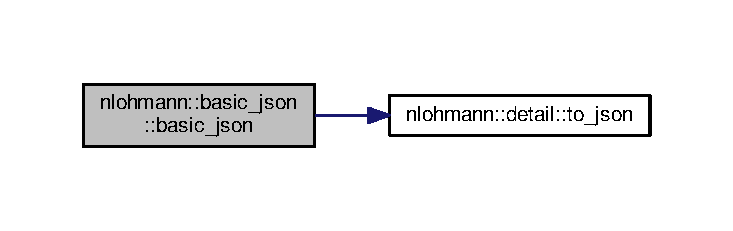
\includegraphics[width=350pt]{classnlohmann_1_1basic__json_a5a6558bfd1be139a638f91f0e09fc737_cgraph}
\end{center}
\end{figure}
\mbox{\Hypertarget{classnlohmann_1_1basic__json_afbad48316e7cd37366ba3ac5d7e5859e}\label{classnlohmann_1_1basic__json_afbad48316e7cd37366ba3ac5d7e5859e}} 
\index{nlohmann\+::basic\+\_\+json@{nlohmann\+::basic\+\_\+json}!basic\+\_\+json@{basic\+\_\+json}}
\index{basic\+\_\+json@{basic\+\_\+json}!nlohmann\+::basic\+\_\+json@{nlohmann\+::basic\+\_\+json}}
\subsubsection{\texorpdfstring{basic\+\_\+json()}{basic\_json()}\hspace{0.1cm}{\footnotesize\ttfamily [4/9]}}
{\footnotesize\ttfamily template$<$template$<$ typename U, typename V, typename... Args $>$ class Object\+Type = std\+::map, template$<$ typename U, typename... Args $>$ class Array\+Type = std\+::vector, class String\+Type  = std\+::string, class Boolean\+Type  = bool, class Number\+Integer\+Type  = std\+::int64\+\_\+t, class Number\+Unsigned\+Type  = std\+::uint64\+\_\+t, class Number\+Float\+Type  = double, template$<$ typename U $>$ class Allocator\+Type = std\+::allocator, template$<$ typename T, typename S\+F\+I\+N\+A\+E=void $>$ class J\+S\+O\+N\+Serializer = adl\+\_\+serializer$>$ \\
\hyperlink{classnlohmann_1_1basic__json}{nlohmann\+::basic\+\_\+json}$<$ Object\+Type, Array\+Type, String\+Type, Boolean\+Type, Number\+Integer\+Type, Number\+Unsigned\+Type, Number\+Float\+Type, Allocator\+Type, J\+S\+O\+N\+Serializer $>$\+::\hyperlink{classnlohmann_1_1basic__json}{basic\+\_\+json} (\begin{DoxyParamCaption}\item[{std\+::initializer\+\_\+list$<$ \hyperlink{classnlohmann_1_1basic__json}{basic\+\_\+json}$<$ Object\+Type, Array\+Type, String\+Type, Boolean\+Type, Number\+Integer\+Type, Number\+Unsigned\+Type, Number\+Float\+Type, Allocator\+Type, J\+S\+O\+N\+Serializer $>$ $>$}]{init,  }\item[{bool}]{type\+\_\+deduction = {\ttfamily true},  }\item[{\hyperlink{namespacenlohmann_1_1detail_a90aa5ef615aa8305e9ea20d8a947980f}{value\+\_\+t}}]{manual\+\_\+type = {\ttfamily \hyperlink{namespacenlohmann_1_1detail_a90aa5ef615aa8305e9ea20d8a947980faf1f713c9e000f5d3f280adbd124df4f5}{value\+\_\+t\+::array}} }\end{DoxyParamCaption})\hspace{0.3cm}{\ttfamily [inline]}}



create a container (array or object) from an initializer list 

Creates a J\+S\+ON value of type array or object from the passed initializer list {\itshape init}. In case {\itshape type\+\_\+deduction} is {\ttfamily true} (default), the type of the J\+S\+ON value to be created is deducted from the initializer list {\itshape init} according to the following rules\+:


\begin{DoxyEnumerate}
\item If the list is empty, an empty J\+S\+ON object value {\ttfamily \{\}} is created.
\item If the list consists of pairs whose first element is a string, a J\+S\+ON object value is created where the first elements of the pairs are treated as keys and the second elements are as values.
\item In all other cases, an array is created.
\end{DoxyEnumerate}

The rules aim to create the best fit between a C++ initializer list and J\+S\+ON values. The rationale is as follows\+:


\begin{DoxyEnumerate}
\item The empty initializer list is written as {\ttfamily \{\}} which is exactly an empty J\+S\+ON object.
\item C++ has now way of describing mapped types other than to list a list of pairs. As J\+S\+ON requires that keys must be of type string, rule 2 is the weakest constraint one can pose on initializer lists to interpret them as an object.
\item In all other cases, the initializer list could not be interpreted as J\+S\+ON object type, so interpreting it as J\+S\+ON array type is safe.
\end{DoxyEnumerate}

With the rules described above, the following J\+S\+ON values cannot be expressed by an initializer list\+:


\begin{DoxyItemize}
\item the empty array ({\ttfamily \mbox{[}\mbox{]}})\+: use \hyperlink{classnlohmann_1_1basic__json_a4a4ec75e4d2845d9bcf7a9e5458e4949}{array(std\+::initializer\+\_\+list$<$basic\+\_\+json$>$)} with an empty initializer list in this case
\item arrays whose elements satisfy rule 2\+: use \hyperlink{classnlohmann_1_1basic__json_a4a4ec75e4d2845d9bcf7a9e5458e4949}{array(std\+::initializer\+\_\+list$<$basic\+\_\+json$>$)} with the same initializer list in this case
\end{DoxyItemize}

\begin{DoxyNote}{Note}
When used without parentheses around an empty initializer list, \hyperlink{classnlohmann_1_1basic__json_a32124a16dc80729d964d9caf607c2bc8}{basic\+\_\+json()} is called instead of this function, yielding the J\+S\+ON null value.
\end{DoxyNote}

\begin{DoxyParams}[1]{Parameters}
\mbox{\tt in}  & {\em init} & initializer list with J\+S\+ON values\\
\hline
\mbox{\tt in}  & {\em type\+\_\+deduction} & internal parameter; when set to {\ttfamily true}, the type of the J\+S\+ON value is deducted from the initializer list {\itshape init}; when set to {\ttfamily false}, the type provided via {\itshape manual\+\_\+type} is forced. This mode is used by the functions \hyperlink{classnlohmann_1_1basic__json_a4a4ec75e4d2845d9bcf7a9e5458e4949}{array(std\+::initializer\+\_\+list$<$basic\+\_\+json$>$)} and \hyperlink{classnlohmann_1_1basic__json_a9f42ee7d10eee2d5a73fd94ca7f767ca}{object(std\+::initializer\+\_\+list$<$basic\+\_\+json$>$)}.\\
\hline
\mbox{\tt in}  & {\em manual\+\_\+type} & internal parameter; when {\itshape type\+\_\+deduction} is set to {\ttfamily false}, the created J\+S\+ON value will use the provided type (only \hyperlink{namespacenlohmann_1_1detail_a90aa5ef615aa8305e9ea20d8a947980faf1f713c9e000f5d3f280adbd124df4f5}{value\+\_\+t\+::array} and \hyperlink{namespacenlohmann_1_1detail_a90aa5ef615aa8305e9ea20d8a947980faa8cfde6331bd59eb2ac96f8911c4b666}{value\+\_\+t\+::object} are valid); when {\itshape type\+\_\+deduction} is set to {\ttfamily true}, this parameter has no effect\\
\hline
\end{DoxyParams}

\begin{DoxyExceptions}{Exceptions}
{\em std\+::domain\+\_\+error} & if {\itshape type\+\_\+deduction} is {\ttfamily false}, {\itshape manual\+\_\+type} is {\ttfamily \hyperlink{namespacenlohmann_1_1detail_a90aa5ef615aa8305e9ea20d8a947980faa8cfde6331bd59eb2ac96f8911c4b666}{value\+\_\+t\+::object}}, but {\itshape init} contains an element which is not a pair whose first element is a string; example\+: {\ttfamily \char`\"{}cannot create object from
initializer list\char`\"{}}\\
\hline
\end{DoxyExceptions}
Linear in the size of the initializer list {\itshape init}.

\{The example below shows how J\+S\+ON values are created from initializer lists.,basic\+\_\+json\+\_\+\+\_\+list\+\_\+init\+\_\+t\}

\begin{DoxySeeAlso}{See also}
\hyperlink{classnlohmann_1_1basic__json_a4a4ec75e4d2845d9bcf7a9e5458e4949}{array(std\+::initializer\+\_\+list$<$basic\+\_\+json$>$)} -- \hyperlink{classnlohmann_1_1basic__json_a81100399cf3e2be457937be7db3f5729}{create} a J\+S\+ON \hyperlink{classnlohmann_1_1basic__json_a4a4ec75e4d2845d9bcf7a9e5458e4949}{array} \hyperlink{classnlohmann_1_1basic__json_af9c51328fbe1da75eca750be3009917a}{value} from an initializer list 

\hyperlink{classnlohmann_1_1basic__json_a9f42ee7d10eee2d5a73fd94ca7f767ca}{object(std\+::initializer\+\_\+list$<$basic\+\_\+json$>$)} -- \hyperlink{classnlohmann_1_1basic__json_a81100399cf3e2be457937be7db3f5729}{create} a J\+S\+ON \hyperlink{classnlohmann_1_1basic__json_a9f42ee7d10eee2d5a73fd94ca7f767ca}{object} \hyperlink{classnlohmann_1_1basic__json_af9c51328fbe1da75eca750be3009917a}{value} from an initializer list
\end{DoxySeeAlso}
\begin{DoxySince}{Since}
version 1.\+0.\+0 
\end{DoxySince}
\mbox{\Hypertarget{classnlohmann_1_1basic__json_ab6816ae5100409254ed0a8bc21c387bb}\label{classnlohmann_1_1basic__json_ab6816ae5100409254ed0a8bc21c387bb}} 
\index{nlohmann\+::basic\+\_\+json@{nlohmann\+::basic\+\_\+json}!basic\+\_\+json@{basic\+\_\+json}}
\index{basic\+\_\+json@{basic\+\_\+json}!nlohmann\+::basic\+\_\+json@{nlohmann\+::basic\+\_\+json}}
\subsubsection{\texorpdfstring{basic\+\_\+json()}{basic\_json()}\hspace{0.1cm}{\footnotesize\ttfamily [5/9]}}
{\footnotesize\ttfamily template$<$template$<$ typename U, typename V, typename... Args $>$ class Object\+Type = std\+::map, template$<$ typename U, typename... Args $>$ class Array\+Type = std\+::vector, class String\+Type  = std\+::string, class Boolean\+Type  = bool, class Number\+Integer\+Type  = std\+::int64\+\_\+t, class Number\+Unsigned\+Type  = std\+::uint64\+\_\+t, class Number\+Float\+Type  = double, template$<$ typename U $>$ class Allocator\+Type = std\+::allocator, template$<$ typename T, typename S\+F\+I\+N\+A\+E=void $>$ class J\+S\+O\+N\+Serializer = adl\+\_\+serializer$>$ \\
\hyperlink{classnlohmann_1_1basic__json}{nlohmann\+::basic\+\_\+json}$<$ Object\+Type, Array\+Type, String\+Type, Boolean\+Type, Number\+Integer\+Type, Number\+Unsigned\+Type, Number\+Float\+Type, Allocator\+Type, J\+S\+O\+N\+Serializer $>$\+::\hyperlink{classnlohmann_1_1basic__json}{basic\+\_\+json} (\begin{DoxyParamCaption}\item[{\hyperlink{classnlohmann_1_1basic__json_a39f2cd0b58106097e0e67bf185cc519b}{size\+\_\+type}}]{cnt,  }\item[{const \hyperlink{classnlohmann_1_1basic__json}{basic\+\_\+json}$<$ Object\+Type, Array\+Type, String\+Type, Boolean\+Type, Number\+Integer\+Type, Number\+Unsigned\+Type, Number\+Float\+Type, Allocator\+Type, J\+S\+O\+N\+Serializer $>$ \&}]{val }\end{DoxyParamCaption})\hspace{0.3cm}{\ttfamily [inline]}}



construct an array with count copies of given value 

Constructs a J\+S\+ON array value by creating {\itshape cnt} copies of a passed value. In case {\itshape cnt} is {\ttfamily 0}, an empty array is created. As postcondition, {\ttfamily std\+::distance(\hyperlink{classnlohmann_1_1basic__json_a0ff28dac23f2bdecee9564d07f51dcdc}{begin()},\hyperlink{classnlohmann_1_1basic__json_a13e032a02a7fd8a93fdddc2fcbc4763c}{end()}) == cnt} holds.


\begin{DoxyParams}[1]{Parameters}
\mbox{\tt in}  & {\em cnt} & the number of J\+S\+ON copies of {\itshape val} to create \\
\hline
\mbox{\tt in}  & {\em val} & the J\+S\+ON value to copy\\
\hline
\end{DoxyParams}
Linear in {\itshape cnt}.

\{The following code shows examples for the \hyperlink{classnlohmann_1_1basic__json}{basic\+\_\+json}(size\+\_\+type\textbackslash{}, const \hyperlink{classnlohmann_1_1basic__json}{basic\+\_\+json}\&) constructor.,basic\+\_\+json\+\_\+\+\_\+size\+\_\+type\+\_\+basic\+\_\+json\}

\begin{DoxySince}{Since}
version 1.\+0.\+0 
\end{DoxySince}
\mbox{\Hypertarget{classnlohmann_1_1basic__json_abe197e9f3184487805cfb5bba6fd5938}\label{classnlohmann_1_1basic__json_abe197e9f3184487805cfb5bba6fd5938}} 
\index{nlohmann\+::basic\+\_\+json@{nlohmann\+::basic\+\_\+json}!basic\+\_\+json@{basic\+\_\+json}}
\index{basic\+\_\+json@{basic\+\_\+json}!nlohmann\+::basic\+\_\+json@{nlohmann\+::basic\+\_\+json}}
\subsubsection{\texorpdfstring{basic\+\_\+json()}{basic\_json()}\hspace{0.1cm}{\footnotesize\ttfamily [6/9]}}
{\footnotesize\ttfamily template$<$template$<$ typename U, typename V, typename... Args $>$ class Object\+Type = std\+::map, template$<$ typename U, typename... Args $>$ class Array\+Type = std\+::vector, class String\+Type  = std\+::string, class Boolean\+Type  = bool, class Number\+Integer\+Type  = std\+::int64\+\_\+t, class Number\+Unsigned\+Type  = std\+::uint64\+\_\+t, class Number\+Float\+Type  = double, template$<$ typename U $>$ class Allocator\+Type = std\+::allocator, template$<$ typename T, typename S\+F\+I\+N\+A\+E=void $>$ class J\+S\+O\+N\+Serializer = adl\+\_\+serializer$>$ \\
template$<$class Input\+IT , typename std\+::enable\+\_\+if$<$ std\+::is\+\_\+same$<$ Input\+I\+T, typename basic\+\_\+json\+\_\+t\+::iterator $>$\+::value or std\+::is\+\_\+same$<$ Input\+I\+T, typename basic\+\_\+json\+\_\+t\+::const\+\_\+iterator $>$\+::value, int $>$\+::type  = 0$>$ \\
\hyperlink{classnlohmann_1_1basic__json}{nlohmann\+::basic\+\_\+json}$<$ Object\+Type, Array\+Type, String\+Type, Boolean\+Type, Number\+Integer\+Type, Number\+Unsigned\+Type, Number\+Float\+Type, Allocator\+Type, J\+S\+O\+N\+Serializer $>$\+::\hyperlink{classnlohmann_1_1basic__json}{basic\+\_\+json} (\begin{DoxyParamCaption}\item[{Input\+IT}]{first,  }\item[{Input\+IT}]{last }\end{DoxyParamCaption})\hspace{0.3cm}{\ttfamily [inline]}}



construct a J\+S\+ON container given an iterator range 

Constructs the J\+S\+ON value with the contents of the range {\ttfamily \mbox{[}first, last)}. The semantics depends on the different types a J\+S\+ON value can have\+:
\begin{DoxyItemize}
\item In case of primitive types (number, boolean, or string), {\itshape first} must be {\ttfamily \hyperlink{classnlohmann_1_1basic__json_a0ff28dac23f2bdecee9564d07f51dcdc}{begin()}} and {\itshape last} must be {\ttfamily \hyperlink{classnlohmann_1_1basic__json_a13e032a02a7fd8a93fdddc2fcbc4763c}{end()}}. In this case, the value is copied. Otherwise, std\+::out\+\_\+of\+\_\+range is thrown.
\item In case of structured types (array, object), the constructor behaves as similar versions for {\ttfamily std\+::vector}.
\item In case of a null type, std\+::domain\+\_\+error is thrown.
\end{DoxyItemize}


\begin{DoxyTemplParams}{Template Parameters}
{\em Input\+IT} & an input iterator type (\hyperlink{classnlohmann_1_1basic__json_a099316232c76c034030a38faa6e34dca}{iterator} or \hyperlink{classnlohmann_1_1basic__json_a41a70cf9993951836d129bb1c2b3126a}{const\+\_\+iterator})\\
\hline
\end{DoxyTemplParams}

\begin{DoxyParams}[1]{Parameters}
\mbox{\tt in}  & {\em first} & begin of the range to copy from (included) \\
\hline
\mbox{\tt in}  & {\em last} & end of the range to copy from (excluded)\\
\hline
\end{DoxyParams}
\begin{DoxyPrecond}{Precondition}
Iterators {\itshape first} and {\itshape last} must be initialized. {\bfseries This precondition is enforced with an assertion.}
\end{DoxyPrecond}

\begin{DoxyExceptions}{Exceptions}
{\em std\+::domain\+\_\+error} & if iterators are not compatible; that is, do not belong to the same J\+S\+ON value; example\+: {\ttfamily \char`\"{}iterators are not compatible\char`\"{}} \\
\hline
{\em std\+::out\+\_\+of\+\_\+range} & if iterators are for a primitive type (number, boolean, or string) where an out of range error can be detected easily; example\+: {\ttfamily \char`\"{}iterators out of range\char`\"{}} \\
\hline
{\em std\+::bad\+\_\+alloc} & if allocation for object, array, or string fails \\
\hline
{\em std\+::domain\+\_\+error} & if called with a null value; example\+: {\ttfamily \char`\"{}cannot
use construct with iterators from null\char`\"{}}\\
\hline
\end{DoxyExceptions}
Linear in distance between {\itshape first} and {\itshape last}.

\{The example below shows several ways to create J\+S\+ON values by specifying a subrange with iterators.,basic\+\_\+json\+\_\+\+\_\+\+Input\+It\+\_\+\+Input\+It\}

\begin{DoxySince}{Since}
version 1.\+0.\+0 
\end{DoxySince}
\mbox{\Hypertarget{classnlohmann_1_1basic__json_a757e90574a742ae9cc54c97422fb3043}\label{classnlohmann_1_1basic__json_a757e90574a742ae9cc54c97422fb3043}} 
\index{nlohmann\+::basic\+\_\+json@{nlohmann\+::basic\+\_\+json}!basic\+\_\+json@{basic\+\_\+json}}
\index{basic\+\_\+json@{basic\+\_\+json}!nlohmann\+::basic\+\_\+json@{nlohmann\+::basic\+\_\+json}}
\subsubsection{\texorpdfstring{basic\+\_\+json()}{basic\_json()}\hspace{0.1cm}{\footnotesize\ttfamily [7/9]}}
{\footnotesize\ttfamily template$<$template$<$ typename U, typename V, typename... Args $>$ class Object\+Type = std\+::map, template$<$ typename U, typename... Args $>$ class Array\+Type = std\+::vector, class String\+Type  = std\+::string, class Boolean\+Type  = bool, class Number\+Integer\+Type  = std\+::int64\+\_\+t, class Number\+Unsigned\+Type  = std\+::uint64\+\_\+t, class Number\+Float\+Type  = double, template$<$ typename U $>$ class Allocator\+Type = std\+::allocator, template$<$ typename T, typename S\+F\+I\+N\+A\+E=void $>$ class J\+S\+O\+N\+Serializer = adl\+\_\+serializer$>$ \\
\hyperlink{json_8hpp_a584fd8f49cd7f4ecf5baba15b5b53cdd}{J\+S\+O\+N\+\_\+\+D\+E\+P\+R\+E\+C\+A\+T\+ED} \hyperlink{classnlohmann_1_1basic__json}{nlohmann\+::basic\+\_\+json}$<$ Object\+Type, Array\+Type, String\+Type, Boolean\+Type, Number\+Integer\+Type, Number\+Unsigned\+Type, Number\+Float\+Type, Allocator\+Type, J\+S\+O\+N\+Serializer $>$\+::\hyperlink{classnlohmann_1_1basic__json}{basic\+\_\+json} (\begin{DoxyParamCaption}\item[{std\+::istream \&}]{i,  }\item[{const \hyperlink{classnlohmann_1_1basic__json_aecae491e175f8767c550ae3c59e180e3}{parser\+\_\+callback\+\_\+t}}]{cb = {\ttfamily nullptr} }\end{DoxyParamCaption})\hspace{0.3cm}{\ttfamily [inline]}, {\ttfamily [explicit]}}



construct a J\+S\+ON value given an input stream 


\begin{DoxyParams}[1]{Parameters}
\mbox{\tt in,out}  & {\em i} & stream to read a serialized J\+S\+ON value from \\
\hline
\mbox{\tt in}  & {\em cb} & a parser callback function of type \hyperlink{classnlohmann_1_1basic__json_aecae491e175f8767c550ae3c59e180e3}{parser\+\_\+callback\+\_\+t} which is used to control the deserialization by filtering unwanted values (optional)\\
\hline
\end{DoxyParams}
Linear in the length of the input. The parser is a predictive L\+L(1) parser. The complexity can be higher if the parser callback function {\itshape cb} has a super-\/linear complexity.

\begin{DoxyNote}{Note}
A U\+T\+F-\/8 byte order mark is silently ignored.
\end{DoxyNote}
\begin{DoxyRefDesc}{Deprecated}
\item[\hyperlink{deprecated__deprecated000001}{Deprecated}]This constructor is deprecated and will be removed in version 3.\+0.\+0 to unify the interface of the library. Deserialization will be done by stream operators or by calling one of the {\ttfamily parse} functions, e.\+g. \hyperlink{classnlohmann_1_1basic__json_a4cd30efe5c33a7cf73a0c6495bb16054}{parse(std\+::istream\&, const parser\+\_\+callback\+\_\+t)}. That is, calls like {\ttfamily json j(i);} for an input stream {\itshape i} need to be replaced by {\ttfamily json j = json\+::parse(i);}. See the example below.\end{DoxyRefDesc}


\{The example below demonstrates constructing a J\+S\+ON value from a {\ttfamily std\+::stringstream} with and without callback function.,basic\+\_\+json\+\_\+\+\_\+istream\}

\begin{DoxySince}{Since}
version 2.\+0.\+0, deprecated in version 2.\+0.\+3, to be removed in version 3.\+0.\+0 
\end{DoxySince}
Here is the call graph for this function\+:\nopagebreak
\begin{figure}[H]
\begin{center}
\leavevmode
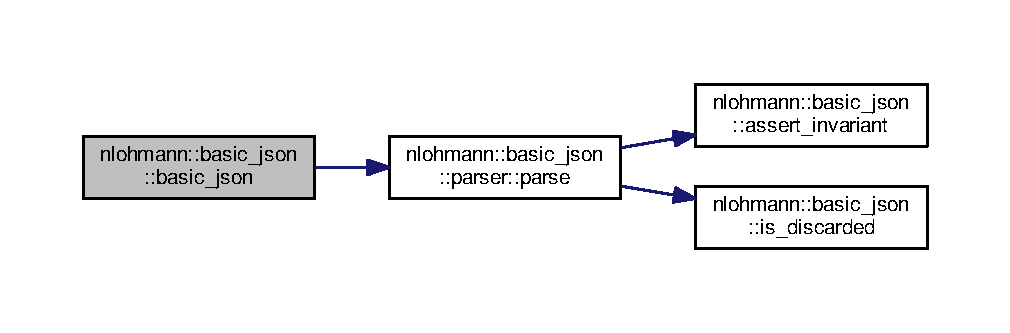
\includegraphics[width=350pt]{classnlohmann_1_1basic__json_a757e90574a742ae9cc54c97422fb3043_cgraph}
\end{center}
\end{figure}
\mbox{\Hypertarget{classnlohmann_1_1basic__json_af5de621bcf646c332343f9c1e011126c}\label{classnlohmann_1_1basic__json_af5de621bcf646c332343f9c1e011126c}} 
\index{nlohmann\+::basic\+\_\+json@{nlohmann\+::basic\+\_\+json}!basic\+\_\+json@{basic\+\_\+json}}
\index{basic\+\_\+json@{basic\+\_\+json}!nlohmann\+::basic\+\_\+json@{nlohmann\+::basic\+\_\+json}}
\subsubsection{\texorpdfstring{basic\+\_\+json()}{basic\_json()}\hspace{0.1cm}{\footnotesize\ttfamily [8/9]}}
{\footnotesize\ttfamily template$<$template$<$ typename U, typename V, typename... Args $>$ class Object\+Type = std\+::map, template$<$ typename U, typename... Args $>$ class Array\+Type = std\+::vector, class String\+Type  = std\+::string, class Boolean\+Type  = bool, class Number\+Integer\+Type  = std\+::int64\+\_\+t, class Number\+Unsigned\+Type  = std\+::uint64\+\_\+t, class Number\+Float\+Type  = double, template$<$ typename U $>$ class Allocator\+Type = std\+::allocator, template$<$ typename T, typename S\+F\+I\+N\+A\+E=void $>$ class J\+S\+O\+N\+Serializer = adl\+\_\+serializer$>$ \\
\hyperlink{classnlohmann_1_1basic__json}{nlohmann\+::basic\+\_\+json}$<$ Object\+Type, Array\+Type, String\+Type, Boolean\+Type, Number\+Integer\+Type, Number\+Unsigned\+Type, Number\+Float\+Type, Allocator\+Type, J\+S\+O\+N\+Serializer $>$\+::\hyperlink{classnlohmann_1_1basic__json}{basic\+\_\+json} (\begin{DoxyParamCaption}\item[{const \hyperlink{classnlohmann_1_1basic__json}{basic\+\_\+json}$<$ Object\+Type, Array\+Type, String\+Type, Boolean\+Type, Number\+Integer\+Type, Number\+Unsigned\+Type, Number\+Float\+Type, Allocator\+Type, J\+S\+O\+N\+Serializer $>$ \&}]{other }\end{DoxyParamCaption})\hspace{0.3cm}{\ttfamily [inline]}}



copy constructor 

Creates a copy of a given J\+S\+ON value.


\begin{DoxyParams}[1]{Parameters}
\mbox{\tt in}  & {\em other} & the J\+S\+ON value to copy\\
\hline
\end{DoxyParams}
Linear in the size of {\itshape other}.

This function helps {\ttfamily \hyperlink{classnlohmann_1_1basic__json}{basic\+\_\+json}} satisfying the \href{http://en.cppreference.com/w/cpp/concept/Container}{\tt Container} requirements\+:
\begin{DoxyItemize}
\item The complexity is linear.
\item As postcondition, it holds\+: {\ttfamily other == basic\+\_\+json(other)}.
\end{DoxyItemize}


\begin{DoxyExceptions}{Exceptions}
{\em std\+::bad\+\_\+alloc} & if allocation for object, array, or string fails.\\
\hline
\end{DoxyExceptions}
\{The following code shows an example for the copy constructor.,basic\+\_\+json\+\_\+\+\_\+basic\+\_\+json\}

\begin{DoxySince}{Since}
version 1.\+0.\+0 
\end{DoxySince}
Here is the call graph for this function\+:\nopagebreak
\begin{figure}[H]
\begin{center}
\leavevmode
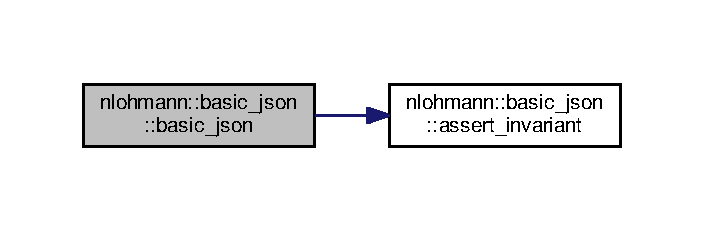
\includegraphics[width=338pt]{classnlohmann_1_1basic__json_af5de621bcf646c332343f9c1e011126c_cgraph}
\end{center}
\end{figure}
\mbox{\Hypertarget{classnlohmann_1_1basic__json_a9a06d1efd50a00f4889f831f851ce124}\label{classnlohmann_1_1basic__json_a9a06d1efd50a00f4889f831f851ce124}} 
\index{nlohmann\+::basic\+\_\+json@{nlohmann\+::basic\+\_\+json}!basic\+\_\+json@{basic\+\_\+json}}
\index{basic\+\_\+json@{basic\+\_\+json}!nlohmann\+::basic\+\_\+json@{nlohmann\+::basic\+\_\+json}}
\subsubsection{\texorpdfstring{basic\+\_\+json()}{basic\_json()}\hspace{0.1cm}{\footnotesize\ttfamily [9/9]}}
{\footnotesize\ttfamily template$<$template$<$ typename U, typename V, typename... Args $>$ class Object\+Type = std\+::map, template$<$ typename U, typename... Args $>$ class Array\+Type = std\+::vector, class String\+Type  = std\+::string, class Boolean\+Type  = bool, class Number\+Integer\+Type  = std\+::int64\+\_\+t, class Number\+Unsigned\+Type  = std\+::uint64\+\_\+t, class Number\+Float\+Type  = double, template$<$ typename U $>$ class Allocator\+Type = std\+::allocator, template$<$ typename T, typename S\+F\+I\+N\+A\+E=void $>$ class J\+S\+O\+N\+Serializer = adl\+\_\+serializer$>$ \\
\hyperlink{classnlohmann_1_1basic__json}{nlohmann\+::basic\+\_\+json}$<$ Object\+Type, Array\+Type, String\+Type, Boolean\+Type, Number\+Integer\+Type, Number\+Unsigned\+Type, Number\+Float\+Type, Allocator\+Type, J\+S\+O\+N\+Serializer $>$\+::\hyperlink{classnlohmann_1_1basic__json}{basic\+\_\+json} (\begin{DoxyParamCaption}\item[{\hyperlink{classnlohmann_1_1basic__json}{basic\+\_\+json}$<$ Object\+Type, Array\+Type, String\+Type, Boolean\+Type, Number\+Integer\+Type, Number\+Unsigned\+Type, Number\+Float\+Type, Allocator\+Type, J\+S\+O\+N\+Serializer $>$ \&\&}]{other }\end{DoxyParamCaption})\hspace{0.3cm}{\ttfamily [inline]}, {\ttfamily [noexcept]}}



move constructor 

Move constructor. Constructs a J\+S\+ON value with the contents of the given value {\itshape other} using move semantics. It \char`\"{}steals\char`\"{} the resources from {\itshape other} and leaves it as J\+S\+ON null value.


\begin{DoxyParams}[1]{Parameters}
\mbox{\tt in,out}  & {\em other} & value to move to this object\\
\hline
\end{DoxyParams}
\begin{DoxyPostcond}{Postcondition}
{\itshape other} is a J\+S\+ON null value
\end{DoxyPostcond}
Constant.

\{The code below shows the move constructor explicitly called via std\+::move.,basic\+\_\+json\+\_\+\+\_\+moveconstructor\}

\begin{DoxySince}{Since}
version 1.\+0.\+0 
\end{DoxySince}
\mbox{\Hypertarget{classnlohmann_1_1basic__json_a42347bbce75ba5571e292a3540af30e0}\label{classnlohmann_1_1basic__json_a42347bbce75ba5571e292a3540af30e0}} 
\index{nlohmann\+::basic\+\_\+json@{nlohmann\+::basic\+\_\+json}!````~basic\+\_\+json@{$\sim$basic\+\_\+json}}
\index{````~basic\+\_\+json@{$\sim$basic\+\_\+json}!nlohmann\+::basic\+\_\+json@{nlohmann\+::basic\+\_\+json}}
\subsubsection{\texorpdfstring{$\sim$basic\+\_\+json()}{~basic\_json()}}
{\footnotesize\ttfamily template$<$template$<$ typename U, typename V, typename... Args $>$ class Object\+Type = std\+::map, template$<$ typename U, typename... Args $>$ class Array\+Type = std\+::vector, class String\+Type  = std\+::string, class Boolean\+Type  = bool, class Number\+Integer\+Type  = std\+::int64\+\_\+t, class Number\+Unsigned\+Type  = std\+::uint64\+\_\+t, class Number\+Float\+Type  = double, template$<$ typename U $>$ class Allocator\+Type = std\+::allocator, template$<$ typename T, typename S\+F\+I\+N\+A\+E=void $>$ class J\+S\+O\+N\+Serializer = adl\+\_\+serializer$>$ \\
\hyperlink{classnlohmann_1_1basic__json}{nlohmann\+::basic\+\_\+json}$<$ Object\+Type, Array\+Type, String\+Type, Boolean\+Type, Number\+Integer\+Type, Number\+Unsigned\+Type, Number\+Float\+Type, Allocator\+Type, J\+S\+O\+N\+Serializer $>$\+::$\sim$\hyperlink{classnlohmann_1_1basic__json}{basic\+\_\+json} (\begin{DoxyParamCaption}{ }\end{DoxyParamCaption})\hspace{0.3cm}{\ttfamily [inline]}}



destructor 

Destroys the J\+S\+ON value and frees all allocated memory.

Linear.

This function helps {\ttfamily \hyperlink{classnlohmann_1_1basic__json}{basic\+\_\+json}} satisfying the \href{http://en.cppreference.com/w/cpp/concept/Container}{\tt Container} requirements\+:
\begin{DoxyItemize}
\item The complexity is linear.
\item All stored elements are destroyed and all memory is freed.
\end{DoxyItemize}

\begin{DoxySince}{Since}
version 1.\+0.\+0 
\end{DoxySince}


\subsection{Member Function Documentation}
\mbox{\Hypertarget{classnlohmann_1_1basic__json_a3fba1efdaca78397efe8ee9e9816b93d}\label{classnlohmann_1_1basic__json_a3fba1efdaca78397efe8ee9e9816b93d}} 
\index{nlohmann\+::basic\+\_\+json@{nlohmann\+::basic\+\_\+json}!add\+\_\+to\+\_\+vector@{add\+\_\+to\+\_\+vector}}
\index{add\+\_\+to\+\_\+vector@{add\+\_\+to\+\_\+vector}!nlohmann\+::basic\+\_\+json@{nlohmann\+::basic\+\_\+json}}
\subsubsection{\texorpdfstring{add\+\_\+to\+\_\+vector()}{add\_to\_vector()}}
{\footnotesize\ttfamily template$<$template$<$ typename U, typename V, typename... Args $>$ class Object\+Type = std\+::map, template$<$ typename U, typename... Args $>$ class Array\+Type = std\+::vector, class String\+Type  = std\+::string, class Boolean\+Type  = bool, class Number\+Integer\+Type  = std\+::int64\+\_\+t, class Number\+Unsigned\+Type  = std\+::uint64\+\_\+t, class Number\+Float\+Type  = double, template$<$ typename U $>$ class Allocator\+Type = std\+::allocator, template$<$ typename T, typename S\+F\+I\+N\+A\+E=void $>$ class J\+S\+O\+N\+Serializer = adl\+\_\+serializer$>$ \\
template$<$typename T $>$ \\
static void \hyperlink{classnlohmann_1_1basic__json}{nlohmann\+::basic\+\_\+json}$<$ Object\+Type, Array\+Type, String\+Type, Boolean\+Type, Number\+Integer\+Type, Number\+Unsigned\+Type, Number\+Float\+Type, Allocator\+Type, J\+S\+O\+N\+Serializer $>$\+::add\+\_\+to\+\_\+vector (\begin{DoxyParamCaption}\item[{std\+::vector$<$ uint8\+\_\+t $>$ \&}]{vec,  }\item[{size\+\_\+t}]{bytes,  }\item[{const T}]{number }\end{DoxyParamCaption})\hspace{0.3cm}{\ttfamily [inline]}, {\ttfamily [static]}, {\ttfamily [private]}}

\begin{DoxyNote}{Note}
Some code in the switch cases has been copied, because otherwise copilers would complain about implicit fallthrough and there is no portable attribute to mute such warnings. 
\end{DoxyNote}
\mbox{\Hypertarget{classnlohmann_1_1basic__json_a4a4ec75e4d2845d9bcf7a9e5458e4949}\label{classnlohmann_1_1basic__json_a4a4ec75e4d2845d9bcf7a9e5458e4949}} 
\index{nlohmann\+::basic\+\_\+json@{nlohmann\+::basic\+\_\+json}!array@{array}}
\index{array@{array}!nlohmann\+::basic\+\_\+json@{nlohmann\+::basic\+\_\+json}}
\subsubsection{\texorpdfstring{array()}{array()}}
{\footnotesize\ttfamily template$<$template$<$ typename U, typename V, typename... Args $>$ class Object\+Type = std\+::map, template$<$ typename U, typename... Args $>$ class Array\+Type = std\+::vector, class String\+Type  = std\+::string, class Boolean\+Type  = bool, class Number\+Integer\+Type  = std\+::int64\+\_\+t, class Number\+Unsigned\+Type  = std\+::uint64\+\_\+t, class Number\+Float\+Type  = double, template$<$ typename U $>$ class Allocator\+Type = std\+::allocator, template$<$ typename T, typename S\+F\+I\+N\+A\+E=void $>$ class J\+S\+O\+N\+Serializer = adl\+\_\+serializer$>$ \\
static \hyperlink{classnlohmann_1_1basic__json}{basic\+\_\+json} \hyperlink{classnlohmann_1_1basic__json}{nlohmann\+::basic\+\_\+json}$<$ Object\+Type, Array\+Type, String\+Type, Boolean\+Type, Number\+Integer\+Type, Number\+Unsigned\+Type, Number\+Float\+Type, Allocator\+Type, J\+S\+O\+N\+Serializer $>$\+::array (\begin{DoxyParamCaption}\item[{std\+::initializer\+\_\+list$<$ \hyperlink{classnlohmann_1_1basic__json}{basic\+\_\+json}$<$ Object\+Type, Array\+Type, String\+Type, Boolean\+Type, Number\+Integer\+Type, Number\+Unsigned\+Type, Number\+Float\+Type, Allocator\+Type, J\+S\+O\+N\+Serializer $>$ $>$}]{init = {\ttfamily std\+:\+:initializer\+\_\+list$<$\hyperlink{classnlohmann_1_1basic__json}{basic\+\_\+json}$<$~ObjectType,~ArrayType,~StringType,~BooleanType,~NumberIntegerType,~NumberUnsignedType,~NumberFloatType,~AllocatorType,~JSONSerializer~$>$$>$()} }\end{DoxyParamCaption})\hspace{0.3cm}{\ttfamily [inline]}, {\ttfamily [static]}}



explicitly create an array from an initializer list 

Creates a J\+S\+ON array value from a given initializer list. That is, given a list of values {\ttfamily a, b, c}, creates the J\+S\+ON value {\ttfamily \mbox{[}a, b, c\mbox{]}}. If the initializer list is empty, the empty array {\ttfamily \mbox{[}\mbox{]}} is created.

\begin{DoxyNote}{Note}
This function is only needed to express two edge cases that cannot be realized with the initializer list constructor (\hyperlink{classnlohmann_1_1basic__json_afbad48316e7cd37366ba3ac5d7e5859e}{basic\+\_\+json(std\+::initializer\+\_\+list$<$basic\+\_\+json$>$, bool, value\+\_\+t)}). These cases are\+:
\begin{DoxyEnumerate}
\item creating an array whose elements are all pairs whose first element is a string -- in this case, the initializer list constructor would create an object, taking the first elements as keys
\item creating an empty array -- passing the empty initializer list to the initializer list constructor yields an empty object
\end{DoxyEnumerate}
\end{DoxyNote}

\begin{DoxyParams}[1]{Parameters}
\mbox{\tt in}  & {\em init} & initializer list with J\+S\+ON values to create an array from (optional)\\
\hline
\end{DoxyParams}
\begin{DoxyReturn}{Returns}
J\+S\+ON array value
\end{DoxyReturn}
Linear in the size of {\itshape init}.

\{The following code shows an example for the {\ttfamily array} function.,array\}

\begin{DoxySeeAlso}{See also}
\hyperlink{classnlohmann_1_1basic__json_afbad48316e7cd37366ba3ac5d7e5859e}{basic\+\_\+json(std\+::initializer\+\_\+list$<$basic\+\_\+json$>$, bool, value\+\_\+t)} -- \hyperlink{classnlohmann_1_1basic__json_a81100399cf3e2be457937be7db3f5729}{create} a J\+S\+ON \hyperlink{classnlohmann_1_1basic__json_af9c51328fbe1da75eca750be3009917a}{value} from an initializer list 

\hyperlink{classnlohmann_1_1basic__json_a9f42ee7d10eee2d5a73fd94ca7f767ca}{object(std\+::initializer\+\_\+list$<$basic\+\_\+json$>$)} -- \hyperlink{classnlohmann_1_1basic__json_a81100399cf3e2be457937be7db3f5729}{create} a J\+S\+ON \hyperlink{classnlohmann_1_1basic__json_a9f42ee7d10eee2d5a73fd94ca7f767ca}{object} \hyperlink{classnlohmann_1_1basic__json_af9c51328fbe1da75eca750be3009917a}{value} from an initializer list
\end{DoxySeeAlso}
\begin{DoxySince}{Since}
version 1.\+0.\+0 
\end{DoxySince}
\mbox{\Hypertarget{classnlohmann_1_1basic__json_a13453ed62f2b771dea9923119beb4f7c}\label{classnlohmann_1_1basic__json_a13453ed62f2b771dea9923119beb4f7c}} 
\index{nlohmann\+::basic\+\_\+json@{nlohmann\+::basic\+\_\+json}!assert\+\_\+invariant@{assert\+\_\+invariant}}
\index{assert\+\_\+invariant@{assert\+\_\+invariant}!nlohmann\+::basic\+\_\+json@{nlohmann\+::basic\+\_\+json}}
\subsubsection{\texorpdfstring{assert\+\_\+invariant()}{assert\_invariant()}}
{\footnotesize\ttfamily template$<$template$<$ typename U, typename V, typename... Args $>$ class Object\+Type = std\+::map, template$<$ typename U, typename... Args $>$ class Array\+Type = std\+::vector, class String\+Type  = std\+::string, class Boolean\+Type  = bool, class Number\+Integer\+Type  = std\+::int64\+\_\+t, class Number\+Unsigned\+Type  = std\+::uint64\+\_\+t, class Number\+Float\+Type  = double, template$<$ typename U $>$ class Allocator\+Type = std\+::allocator, template$<$ typename T, typename S\+F\+I\+N\+A\+E=void $>$ class J\+S\+O\+N\+Serializer = adl\+\_\+serializer$>$ \\
void \hyperlink{classnlohmann_1_1basic__json}{nlohmann\+::basic\+\_\+json}$<$ Object\+Type, Array\+Type, String\+Type, Boolean\+Type, Number\+Integer\+Type, Number\+Unsigned\+Type, Number\+Float\+Type, Allocator\+Type, J\+S\+O\+N\+Serializer $>$\+::assert\+\_\+invariant (\begin{DoxyParamCaption}{ }\end{DoxyParamCaption}) const\hspace{0.3cm}{\ttfamily [inline]}, {\ttfamily [private]}}



checks the class invariants 

This function asserts the class invariants. It needs to be called at the end of every constructor to make sure that created objects respect the invariant. Furthermore, it has to be called each time the type of a J\+S\+ON value is changed, because the invariant expresses a relationship between {\itshape m\+\_\+type} and {\itshape m\+\_\+value}. \mbox{\Hypertarget{classnlohmann_1_1basic__json_a73ae333487310e3302135189ce8ff5d8}\label{classnlohmann_1_1basic__json_a73ae333487310e3302135189ce8ff5d8}} 
\index{nlohmann\+::basic\+\_\+json@{nlohmann\+::basic\+\_\+json}!at@{at}}
\index{at@{at}!nlohmann\+::basic\+\_\+json@{nlohmann\+::basic\+\_\+json}}
\subsubsection{\texorpdfstring{at()}{at()}\hspace{0.1cm}{\footnotesize\ttfamily [1/6]}}
{\footnotesize\ttfamily template$<$template$<$ typename U, typename V, typename... Args $>$ class Object\+Type = std\+::map, template$<$ typename U, typename... Args $>$ class Array\+Type = std\+::vector, class String\+Type  = std\+::string, class Boolean\+Type  = bool, class Number\+Integer\+Type  = std\+::int64\+\_\+t, class Number\+Unsigned\+Type  = std\+::uint64\+\_\+t, class Number\+Float\+Type  = double, template$<$ typename U $>$ class Allocator\+Type = std\+::allocator, template$<$ typename T, typename S\+F\+I\+N\+A\+E=void $>$ class J\+S\+O\+N\+Serializer = adl\+\_\+serializer$>$ \\
\hyperlink{classnlohmann_1_1basic__json_ac6a5eddd156c776ac75ff54cfe54a5bc}{reference} \hyperlink{classnlohmann_1_1basic__json}{nlohmann\+::basic\+\_\+json}$<$ Object\+Type, Array\+Type, String\+Type, Boolean\+Type, Number\+Integer\+Type, Number\+Unsigned\+Type, Number\+Float\+Type, Allocator\+Type, J\+S\+O\+N\+Serializer $>$\+::at (\begin{DoxyParamCaption}\item[{\hyperlink{classnlohmann_1_1basic__json_a39f2cd0b58106097e0e67bf185cc519b}{size\+\_\+type}}]{idx }\end{DoxyParamCaption})\hspace{0.3cm}{\ttfamily [inline]}}



access specified array element with bounds checking 

Returns a reference to the element at specified location {\itshape idx}, with bounds checking.


\begin{DoxyParams}[1]{Parameters}
\mbox{\tt in}  & {\em idx} & index of the element to access\\
\hline
\end{DoxyParams}
\begin{DoxyReturn}{Returns}
reference to the element at index {\itshape idx} 
\end{DoxyReturn}

\begin{DoxyExceptions}{Exceptions}
{\em std\+::domain\+\_\+error} & if the J\+S\+ON value is not an array; example\+: {\ttfamily \char`\"{}cannot use at() with string\char`\"{}} \\
\hline
{\em std\+::out\+\_\+of\+\_\+range} & if the index {\itshape idx} is out of range of the array; that is, {\ttfamily idx $>$= \hyperlink{classnlohmann_1_1basic__json_a25e27ad0c6d53c01871c5485e1f75b96}{size()}}; example\+: {\ttfamily \char`\"{}array index 7 is out of range\char`\"{}}\\
\hline
\end{DoxyExceptions}
Constant.

\{The example below shows how array elements can be read and written using {\ttfamily \hyperlink{classnlohmann_1_1basic__json_a73ae333487310e3302135189ce8ff5d8}{at()}}.,at\+\_\+\+\_\+size\+\_\+type\}

\begin{DoxySince}{Since}
version 1.\+0.\+0 
\end{DoxySince}
\mbox{\Hypertarget{classnlohmann_1_1basic__json_ab157adb4de8475b452da9ebf04f2de15}\label{classnlohmann_1_1basic__json_ab157adb4de8475b452da9ebf04f2de15}} 
\index{nlohmann\+::basic\+\_\+json@{nlohmann\+::basic\+\_\+json}!at@{at}}
\index{at@{at}!nlohmann\+::basic\+\_\+json@{nlohmann\+::basic\+\_\+json}}
\subsubsection{\texorpdfstring{at()}{at()}\hspace{0.1cm}{\footnotesize\ttfamily [2/6]}}
{\footnotesize\ttfamily template$<$template$<$ typename U, typename V, typename... Args $>$ class Object\+Type = std\+::map, template$<$ typename U, typename... Args $>$ class Array\+Type = std\+::vector, class String\+Type  = std\+::string, class Boolean\+Type  = bool, class Number\+Integer\+Type  = std\+::int64\+\_\+t, class Number\+Unsigned\+Type  = std\+::uint64\+\_\+t, class Number\+Float\+Type  = double, template$<$ typename U $>$ class Allocator\+Type = std\+::allocator, template$<$ typename T, typename S\+F\+I\+N\+A\+E=void $>$ class J\+S\+O\+N\+Serializer = adl\+\_\+serializer$>$ \\
\hyperlink{classnlohmann_1_1basic__json_a4057c5425f4faacfe39a8046871786ca}{const\+\_\+reference} \hyperlink{classnlohmann_1_1basic__json}{nlohmann\+::basic\+\_\+json}$<$ Object\+Type, Array\+Type, String\+Type, Boolean\+Type, Number\+Integer\+Type, Number\+Unsigned\+Type, Number\+Float\+Type, Allocator\+Type, J\+S\+O\+N\+Serializer $>$\+::at (\begin{DoxyParamCaption}\item[{\hyperlink{classnlohmann_1_1basic__json_a39f2cd0b58106097e0e67bf185cc519b}{size\+\_\+type}}]{idx }\end{DoxyParamCaption}) const\hspace{0.3cm}{\ttfamily [inline]}}



access specified array element with bounds checking 

Returns a const reference to the element at specified location {\itshape idx}, with bounds checking.


\begin{DoxyParams}[1]{Parameters}
\mbox{\tt in}  & {\em idx} & index of the element to access\\
\hline
\end{DoxyParams}
\begin{DoxyReturn}{Returns}
const reference to the element at index {\itshape idx} 
\end{DoxyReturn}

\begin{DoxyExceptions}{Exceptions}
{\em std\+::domain\+\_\+error} & if the J\+S\+ON value is not an array; example\+: {\ttfamily \char`\"{}cannot use at() with string\char`\"{}} \\
\hline
{\em std\+::out\+\_\+of\+\_\+range} & if the index {\itshape idx} is out of range of the array; that is, {\ttfamily idx $>$= \hyperlink{classnlohmann_1_1basic__json_a25e27ad0c6d53c01871c5485e1f75b96}{size()}}; example\+: {\ttfamily \char`\"{}array index 7 is out of range\char`\"{}}\\
\hline
\end{DoxyExceptions}
Constant.

\{The example below shows how array elements can be read using {\ttfamily \hyperlink{classnlohmann_1_1basic__json_a73ae333487310e3302135189ce8ff5d8}{at()}}.,at\+\_\+\+\_\+size\+\_\+type\+\_\+const\}

\begin{DoxySince}{Since}
version 1.\+0.\+0 
\end{DoxySince}
\mbox{\Hypertarget{classnlohmann_1_1basic__json_a93403e803947b86f4da2d1fb3345cf2c}\label{classnlohmann_1_1basic__json_a93403e803947b86f4da2d1fb3345cf2c}} 
\index{nlohmann\+::basic\+\_\+json@{nlohmann\+::basic\+\_\+json}!at@{at}}
\index{at@{at}!nlohmann\+::basic\+\_\+json@{nlohmann\+::basic\+\_\+json}}
\subsubsection{\texorpdfstring{at()}{at()}\hspace{0.1cm}{\footnotesize\ttfamily [3/6]}}
{\footnotesize\ttfamily template$<$template$<$ typename U, typename V, typename... Args $>$ class Object\+Type = std\+::map, template$<$ typename U, typename... Args $>$ class Array\+Type = std\+::vector, class String\+Type  = std\+::string, class Boolean\+Type  = bool, class Number\+Integer\+Type  = std\+::int64\+\_\+t, class Number\+Unsigned\+Type  = std\+::uint64\+\_\+t, class Number\+Float\+Type  = double, template$<$ typename U $>$ class Allocator\+Type = std\+::allocator, template$<$ typename T, typename S\+F\+I\+N\+A\+E=void $>$ class J\+S\+O\+N\+Serializer = adl\+\_\+serializer$>$ \\
\hyperlink{classnlohmann_1_1basic__json_ac6a5eddd156c776ac75ff54cfe54a5bc}{reference} \hyperlink{classnlohmann_1_1basic__json}{nlohmann\+::basic\+\_\+json}$<$ Object\+Type, Array\+Type, String\+Type, Boolean\+Type, Number\+Integer\+Type, Number\+Unsigned\+Type, Number\+Float\+Type, Allocator\+Type, J\+S\+O\+N\+Serializer $>$\+::at (\begin{DoxyParamCaption}\item[{const typename object\+\_\+t\+::key\+\_\+type \&}]{key }\end{DoxyParamCaption})\hspace{0.3cm}{\ttfamily [inline]}}



access specified object element with bounds checking 

Returns a reference to the element at with specified key {\itshape key}, with bounds checking.


\begin{DoxyParams}[1]{Parameters}
\mbox{\tt in}  & {\em key} & key of the element to access\\
\hline
\end{DoxyParams}
\begin{DoxyReturn}{Returns}
reference to the element at key {\itshape key} 
\end{DoxyReturn}

\begin{DoxyExceptions}{Exceptions}
{\em std\+::domain\+\_\+error} & if the J\+S\+ON value is not an object; example\+: {\ttfamily \char`\"{}cannot use at() with boolean\char`\"{}} \\
\hline
{\em std\+::out\+\_\+of\+\_\+range} & if the key {\itshape key} is is not stored in the object; that is, {\ttfamily find(key) == \hyperlink{classnlohmann_1_1basic__json_a13e032a02a7fd8a93fdddc2fcbc4763c}{end()}}; example\+: {\ttfamily \char`\"{}key \char`\"{}the fast\char`\"{} not found\char`\"{}}\\
\hline
\end{DoxyExceptions}
Logarithmic in the size of the container.

\{The example below shows how object elements can be read and written using {\ttfamily \hyperlink{classnlohmann_1_1basic__json_a73ae333487310e3302135189ce8ff5d8}{at()}}.,at\+\_\+\+\_\+object\+\_\+t\+\_\+key\+\_\+type\}

\begin{DoxySeeAlso}{See also}
\hyperlink{classnlohmann_1_1basic__json_a233b02b0839ef798942dd46157cc0fe6}{operator\mbox{[}$\,$\mbox{]}(const typename object\+\_\+t\+::key\+\_\+type\&)} for unchecked access by \hyperlink{classnlohmann_1_1basic__json_ac6a5eddd156c776ac75ff54cfe54a5bc}{reference} 

\hyperlink{classnlohmann_1_1basic__json_af9c51328fbe1da75eca750be3009917a}{value()} for access by \hyperlink{classnlohmann_1_1basic__json_af9c51328fbe1da75eca750be3009917a}{value} with a default \hyperlink{classnlohmann_1_1basic__json_af9c51328fbe1da75eca750be3009917a}{value}
\end{DoxySeeAlso}
\begin{DoxySince}{Since}
version 1.\+0.\+0 
\end{DoxySince}
\mbox{\Hypertarget{classnlohmann_1_1basic__json_acac9d438c9bb12740dcdb01069293a34}\label{classnlohmann_1_1basic__json_acac9d438c9bb12740dcdb01069293a34}} 
\index{nlohmann\+::basic\+\_\+json@{nlohmann\+::basic\+\_\+json}!at@{at}}
\index{at@{at}!nlohmann\+::basic\+\_\+json@{nlohmann\+::basic\+\_\+json}}
\subsubsection{\texorpdfstring{at()}{at()}\hspace{0.1cm}{\footnotesize\ttfamily [4/6]}}
{\footnotesize\ttfamily template$<$template$<$ typename U, typename V, typename... Args $>$ class Object\+Type = std\+::map, template$<$ typename U, typename... Args $>$ class Array\+Type = std\+::vector, class String\+Type  = std\+::string, class Boolean\+Type  = bool, class Number\+Integer\+Type  = std\+::int64\+\_\+t, class Number\+Unsigned\+Type  = std\+::uint64\+\_\+t, class Number\+Float\+Type  = double, template$<$ typename U $>$ class Allocator\+Type = std\+::allocator, template$<$ typename T, typename S\+F\+I\+N\+A\+E=void $>$ class J\+S\+O\+N\+Serializer = adl\+\_\+serializer$>$ \\
\hyperlink{classnlohmann_1_1basic__json_a4057c5425f4faacfe39a8046871786ca}{const\+\_\+reference} \hyperlink{classnlohmann_1_1basic__json}{nlohmann\+::basic\+\_\+json}$<$ Object\+Type, Array\+Type, String\+Type, Boolean\+Type, Number\+Integer\+Type, Number\+Unsigned\+Type, Number\+Float\+Type, Allocator\+Type, J\+S\+O\+N\+Serializer $>$\+::at (\begin{DoxyParamCaption}\item[{const typename object\+\_\+t\+::key\+\_\+type \&}]{key }\end{DoxyParamCaption}) const\hspace{0.3cm}{\ttfamily [inline]}}



access specified object element with bounds checking 

Returns a const reference to the element at with specified key {\itshape key}, with bounds checking.


\begin{DoxyParams}[1]{Parameters}
\mbox{\tt in}  & {\em key} & key of the element to access\\
\hline
\end{DoxyParams}
\begin{DoxyReturn}{Returns}
const reference to the element at key {\itshape key} 
\end{DoxyReturn}

\begin{DoxyExceptions}{Exceptions}
{\em std\+::domain\+\_\+error} & if the J\+S\+ON value is not an object; example\+: {\ttfamily \char`\"{}cannot use at() with boolean\char`\"{}} \\
\hline
{\em std\+::out\+\_\+of\+\_\+range} & if the key {\itshape key} is is not stored in the object; that is, {\ttfamily find(key) == \hyperlink{classnlohmann_1_1basic__json_a13e032a02a7fd8a93fdddc2fcbc4763c}{end()}}; example\+: {\ttfamily \char`\"{}key \char`\"{}the fast\char`\"{} not found\char`\"{}}\\
\hline
\end{DoxyExceptions}
Logarithmic in the size of the container.

\{The example below shows how object elements can be read using {\ttfamily \hyperlink{classnlohmann_1_1basic__json_a73ae333487310e3302135189ce8ff5d8}{at()}}.,at\+\_\+\+\_\+object\+\_\+t\+\_\+key\+\_\+type\+\_\+const\}

\begin{DoxySeeAlso}{See also}
\hyperlink{classnlohmann_1_1basic__json_a233b02b0839ef798942dd46157cc0fe6}{operator\mbox{[}$\,$\mbox{]}(const typename object\+\_\+t\+::key\+\_\+type\&)} for unchecked access by \hyperlink{classnlohmann_1_1basic__json_ac6a5eddd156c776ac75ff54cfe54a5bc}{reference} 

\hyperlink{classnlohmann_1_1basic__json_af9c51328fbe1da75eca750be3009917a}{value()} for access by \hyperlink{classnlohmann_1_1basic__json_af9c51328fbe1da75eca750be3009917a}{value} with a default \hyperlink{classnlohmann_1_1basic__json_af9c51328fbe1da75eca750be3009917a}{value}
\end{DoxySeeAlso}
\begin{DoxySince}{Since}
version 1.\+0.\+0 
\end{DoxySince}
\mbox{\Hypertarget{classnlohmann_1_1basic__json_a8ab61397c10f18b305520da7073b2b45}\label{classnlohmann_1_1basic__json_a8ab61397c10f18b305520da7073b2b45}} 
\index{nlohmann\+::basic\+\_\+json@{nlohmann\+::basic\+\_\+json}!at@{at}}
\index{at@{at}!nlohmann\+::basic\+\_\+json@{nlohmann\+::basic\+\_\+json}}
\subsubsection{\texorpdfstring{at()}{at()}\hspace{0.1cm}{\footnotesize\ttfamily [5/6]}}
{\footnotesize\ttfamily template$<$template$<$ typename U, typename V, typename... Args $>$ class Object\+Type = std\+::map, template$<$ typename U, typename... Args $>$ class Array\+Type = std\+::vector, class String\+Type  = std\+::string, class Boolean\+Type  = bool, class Number\+Integer\+Type  = std\+::int64\+\_\+t, class Number\+Unsigned\+Type  = std\+::uint64\+\_\+t, class Number\+Float\+Type  = double, template$<$ typename U $>$ class Allocator\+Type = std\+::allocator, template$<$ typename T, typename S\+F\+I\+N\+A\+E=void $>$ class J\+S\+O\+N\+Serializer = adl\+\_\+serializer$>$ \\
\hyperlink{classnlohmann_1_1basic__json_ac6a5eddd156c776ac75ff54cfe54a5bc}{reference} \hyperlink{classnlohmann_1_1basic__json}{nlohmann\+::basic\+\_\+json}$<$ Object\+Type, Array\+Type, String\+Type, Boolean\+Type, Number\+Integer\+Type, Number\+Unsigned\+Type, Number\+Float\+Type, Allocator\+Type, J\+S\+O\+N\+Serializer $>$\+::at (\begin{DoxyParamCaption}\item[{const \hyperlink{classnlohmann_1_1basic__json_1_1json__pointer}{json\+\_\+pointer} \&}]{ptr }\end{DoxyParamCaption})\hspace{0.3cm}{\ttfamily [inline]}}



access specified element via J\+S\+ON Pointer 

Returns a reference to the element at with specified J\+S\+ON pointer {\itshape ptr}, with bounds checking.


\begin{DoxyParams}[1]{Parameters}
\mbox{\tt in}  & {\em ptr} & J\+S\+ON pointer to the desired element\\
\hline
\end{DoxyParams}
\begin{DoxyReturn}{Returns}
reference to the element pointed to by {\itshape ptr} 
\end{DoxyReturn}
Constant.


\begin{DoxyExceptions}{Exceptions}
{\em std\+::out\+\_\+of\+\_\+range} & if the J\+S\+ON pointer can not be resolved \\
\hline
{\em std\+::domain\+\_\+error} & if an array index begins with \textquotesingle{}0\textquotesingle{} \\
\hline
{\em std\+::invalid\+\_\+argument} & if an array index was not a number\\
\hline
\end{DoxyExceptions}
\{The behavior is shown in the example.,at\+\_\+json\+\_\+pointer\}

\begin{DoxySince}{Since}
version 2.\+0.\+0 
\end{DoxySince}
Here is the call graph for this function\+:\nopagebreak
\begin{figure}[H]
\begin{center}
\leavevmode
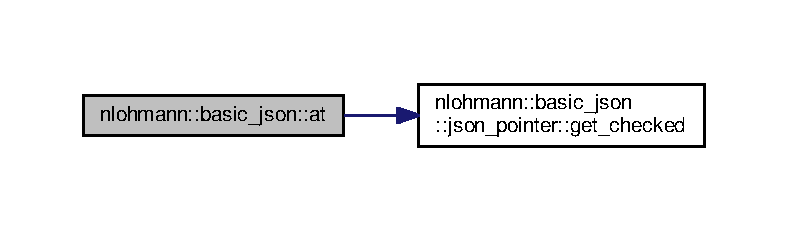
\includegraphics[width=350pt]{classnlohmann_1_1basic__json_a8ab61397c10f18b305520da7073b2b45_cgraph}
\end{center}
\end{figure}
\mbox{\Hypertarget{classnlohmann_1_1basic__json_a7479d686148c26e252781bb32aa5d5c9}\label{classnlohmann_1_1basic__json_a7479d686148c26e252781bb32aa5d5c9}} 
\index{nlohmann\+::basic\+\_\+json@{nlohmann\+::basic\+\_\+json}!at@{at}}
\index{at@{at}!nlohmann\+::basic\+\_\+json@{nlohmann\+::basic\+\_\+json}}
\subsubsection{\texorpdfstring{at()}{at()}\hspace{0.1cm}{\footnotesize\ttfamily [6/6]}}
{\footnotesize\ttfamily template$<$template$<$ typename U, typename V, typename... Args $>$ class Object\+Type = std\+::map, template$<$ typename U, typename... Args $>$ class Array\+Type = std\+::vector, class String\+Type  = std\+::string, class Boolean\+Type  = bool, class Number\+Integer\+Type  = std\+::int64\+\_\+t, class Number\+Unsigned\+Type  = std\+::uint64\+\_\+t, class Number\+Float\+Type  = double, template$<$ typename U $>$ class Allocator\+Type = std\+::allocator, template$<$ typename T, typename S\+F\+I\+N\+A\+E=void $>$ class J\+S\+O\+N\+Serializer = adl\+\_\+serializer$>$ \\
\hyperlink{classnlohmann_1_1basic__json_a4057c5425f4faacfe39a8046871786ca}{const\+\_\+reference} \hyperlink{classnlohmann_1_1basic__json}{nlohmann\+::basic\+\_\+json}$<$ Object\+Type, Array\+Type, String\+Type, Boolean\+Type, Number\+Integer\+Type, Number\+Unsigned\+Type, Number\+Float\+Type, Allocator\+Type, J\+S\+O\+N\+Serializer $>$\+::at (\begin{DoxyParamCaption}\item[{const \hyperlink{classnlohmann_1_1basic__json_1_1json__pointer}{json\+\_\+pointer} \&}]{ptr }\end{DoxyParamCaption}) const\hspace{0.3cm}{\ttfamily [inline]}}



access specified element via J\+S\+ON Pointer 

Returns a const reference to the element at with specified J\+S\+ON pointer {\itshape ptr}, with bounds checking.


\begin{DoxyParams}[1]{Parameters}
\mbox{\tt in}  & {\em ptr} & J\+S\+ON pointer to the desired element\\
\hline
\end{DoxyParams}
\begin{DoxyReturn}{Returns}
reference to the element pointed to by {\itshape ptr} 
\end{DoxyReturn}
Constant.


\begin{DoxyExceptions}{Exceptions}
{\em std\+::out\+\_\+of\+\_\+range} & if the J\+S\+ON pointer can not be resolved \\
\hline
{\em std\+::domain\+\_\+error} & if an array index begins with \textquotesingle{}0\textquotesingle{} \\
\hline
{\em std\+::invalid\+\_\+argument} & if an array index was not a number\\
\hline
\end{DoxyExceptions}
\{The behavior is shown in the example.,at\+\_\+json\+\_\+pointer\+\_\+const\}

\begin{DoxySince}{Since}
version 2.\+0.\+0 
\end{DoxySince}
Here is the call graph for this function\+:\nopagebreak
\begin{figure}[H]
\begin{center}
\leavevmode
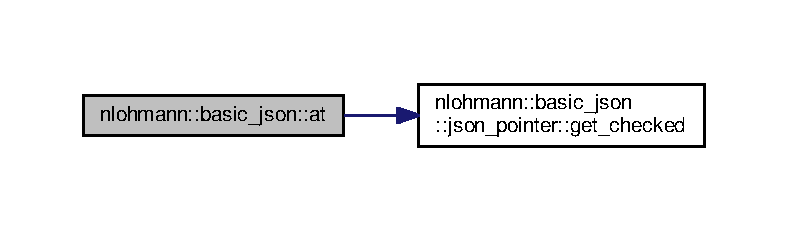
\includegraphics[width=350pt]{classnlohmann_1_1basic__json_a7479d686148c26e252781bb32aa5d5c9_cgraph}
\end{center}
\end{figure}
\mbox{\Hypertarget{classnlohmann_1_1basic__json_a011397134847f36db0ed7d7a93753677}\label{classnlohmann_1_1basic__json_a011397134847f36db0ed7d7a93753677}} 
\index{nlohmann\+::basic\+\_\+json@{nlohmann\+::basic\+\_\+json}!back@{back}}
\index{back@{back}!nlohmann\+::basic\+\_\+json@{nlohmann\+::basic\+\_\+json}}
\subsubsection{\texorpdfstring{back()}{back()}\hspace{0.1cm}{\footnotesize\ttfamily [1/2]}}
{\footnotesize\ttfamily template$<$template$<$ typename U, typename V, typename... Args $>$ class Object\+Type = std\+::map, template$<$ typename U, typename... Args $>$ class Array\+Type = std\+::vector, class String\+Type  = std\+::string, class Boolean\+Type  = bool, class Number\+Integer\+Type  = std\+::int64\+\_\+t, class Number\+Unsigned\+Type  = std\+::uint64\+\_\+t, class Number\+Float\+Type  = double, template$<$ typename U $>$ class Allocator\+Type = std\+::allocator, template$<$ typename T, typename S\+F\+I\+N\+A\+E=void $>$ class J\+S\+O\+N\+Serializer = adl\+\_\+serializer$>$ \\
\hyperlink{classnlohmann_1_1basic__json_ac6a5eddd156c776ac75ff54cfe54a5bc}{reference} \hyperlink{classnlohmann_1_1basic__json}{nlohmann\+::basic\+\_\+json}$<$ Object\+Type, Array\+Type, String\+Type, Boolean\+Type, Number\+Integer\+Type, Number\+Unsigned\+Type, Number\+Float\+Type, Allocator\+Type, J\+S\+O\+N\+Serializer $>$\+::back (\begin{DoxyParamCaption}{ }\end{DoxyParamCaption})\hspace{0.3cm}{\ttfamily [inline]}}



access the last element 

Returns a reference to the last element in the container. For a J\+S\+ON container {\ttfamily c}, the expression {\ttfamily c.\+back()} is equivalent to 
\begin{DoxyCode}
\textcolor{keyword}{auto} tmp = c.end();
--tmp;
\textcolor{keywordflow}{return} *tmp;
\end{DoxyCode}


\begin{DoxyReturn}{Returns}
In case of a structured type (array or object), a reference to the last element is returned. In case of number, string, or boolean values, a reference to the value is returned.
\end{DoxyReturn}
Constant.

\begin{DoxyPrecond}{Precondition}
The J\+S\+ON value must not be {\ttfamily null} (would throw {\ttfamily std\+::out\+\_\+of\+\_\+range}) or an empty array or object (undefined behavior, {\bfseries guarded by assertions}). 
\end{DoxyPrecond}
\begin{DoxyPostcond}{Postcondition}
The J\+S\+ON value remains unchanged.
\end{DoxyPostcond}

\begin{DoxyExceptions}{Exceptions}
{\em std\+::out\+\_\+of\+\_\+range} & when called on {\ttfamily null} value.\\
\hline
\end{DoxyExceptions}
\{The following code shows an example for {\ttfamily \hyperlink{classnlohmann_1_1basic__json_a011397134847f36db0ed7d7a93753677}{back()}}.,back\}

\begin{DoxySeeAlso}{See also}
\hyperlink{classnlohmann_1_1basic__json_a3acba9c6ceb7214e565fe08c3ba5b352}{front()} -- access the first element
\end{DoxySeeAlso}
\begin{DoxySince}{Since}
version 1.\+0.\+0 
\end{DoxySince}
\mbox{\Hypertarget{classnlohmann_1_1basic__json_a83fe4a151b3a591f357527d5d9aa1b9f}\label{classnlohmann_1_1basic__json_a83fe4a151b3a591f357527d5d9aa1b9f}} 
\index{nlohmann\+::basic\+\_\+json@{nlohmann\+::basic\+\_\+json}!back@{back}}
\index{back@{back}!nlohmann\+::basic\+\_\+json@{nlohmann\+::basic\+\_\+json}}
\subsubsection{\texorpdfstring{back()}{back()}\hspace{0.1cm}{\footnotesize\ttfamily [2/2]}}
{\footnotesize\ttfamily template$<$template$<$ typename U, typename V, typename... Args $>$ class Object\+Type = std\+::map, template$<$ typename U, typename... Args $>$ class Array\+Type = std\+::vector, class String\+Type  = std\+::string, class Boolean\+Type  = bool, class Number\+Integer\+Type  = std\+::int64\+\_\+t, class Number\+Unsigned\+Type  = std\+::uint64\+\_\+t, class Number\+Float\+Type  = double, template$<$ typename U $>$ class Allocator\+Type = std\+::allocator, template$<$ typename T, typename S\+F\+I\+N\+A\+E=void $>$ class J\+S\+O\+N\+Serializer = adl\+\_\+serializer$>$ \\
\hyperlink{classnlohmann_1_1basic__json_a4057c5425f4faacfe39a8046871786ca}{const\+\_\+reference} \hyperlink{classnlohmann_1_1basic__json}{nlohmann\+::basic\+\_\+json}$<$ Object\+Type, Array\+Type, String\+Type, Boolean\+Type, Number\+Integer\+Type, Number\+Unsigned\+Type, Number\+Float\+Type, Allocator\+Type, J\+S\+O\+N\+Serializer $>$\+::back (\begin{DoxyParamCaption}{ }\end{DoxyParamCaption}) const\hspace{0.3cm}{\ttfamily [inline]}}



access the last element 

Returns a reference to the last element in the container. For a J\+S\+ON container {\ttfamily c}, the expression {\ttfamily c.\+back()} is equivalent to 
\begin{DoxyCode}
\textcolor{keyword}{auto} tmp = c.end();
--tmp;
\textcolor{keywordflow}{return} *tmp;
\end{DoxyCode}


\begin{DoxyReturn}{Returns}
In case of a structured type (array or object), a reference to the last element is returned. In case of number, string, or boolean values, a reference to the value is returned.
\end{DoxyReturn}
Constant.

\begin{DoxyPrecond}{Precondition}
The J\+S\+ON value must not be {\ttfamily null} (would throw {\ttfamily std\+::out\+\_\+of\+\_\+range}) or an empty array or object (undefined behavior, {\bfseries guarded by assertions}). 
\end{DoxyPrecond}
\begin{DoxyPostcond}{Postcondition}
The J\+S\+ON value remains unchanged.
\end{DoxyPostcond}

\begin{DoxyExceptions}{Exceptions}
{\em std\+::out\+\_\+of\+\_\+range} & when called on {\ttfamily null} value.\\
\hline
\end{DoxyExceptions}
\{The following code shows an example for {\ttfamily \hyperlink{classnlohmann_1_1basic__json_a011397134847f36db0ed7d7a93753677}{back()}}.,back\}

\begin{DoxySeeAlso}{See also}
\hyperlink{classnlohmann_1_1basic__json_a3acba9c6ceb7214e565fe08c3ba5b352}{front()} -- access the first element
\end{DoxySeeAlso}
\begin{DoxySince}{Since}
version 1.\+0.\+0 
\end{DoxySince}
\mbox{\Hypertarget{classnlohmann_1_1basic__json_a0ff28dac23f2bdecee9564d07f51dcdc}\label{classnlohmann_1_1basic__json_a0ff28dac23f2bdecee9564d07f51dcdc}} 
\index{nlohmann\+::basic\+\_\+json@{nlohmann\+::basic\+\_\+json}!begin@{begin}}
\index{begin@{begin}!nlohmann\+::basic\+\_\+json@{nlohmann\+::basic\+\_\+json}}
\subsubsection{\texorpdfstring{begin()}{begin()}\hspace{0.1cm}{\footnotesize\ttfamily [1/2]}}
{\footnotesize\ttfamily template$<$template$<$ typename U, typename V, typename... Args $>$ class Object\+Type = std\+::map, template$<$ typename U, typename... Args $>$ class Array\+Type = std\+::vector, class String\+Type  = std\+::string, class Boolean\+Type  = bool, class Number\+Integer\+Type  = std\+::int64\+\_\+t, class Number\+Unsigned\+Type  = std\+::uint64\+\_\+t, class Number\+Float\+Type  = double, template$<$ typename U $>$ class Allocator\+Type = std\+::allocator, template$<$ typename T, typename S\+F\+I\+N\+A\+E=void $>$ class J\+S\+O\+N\+Serializer = adl\+\_\+serializer$>$ \\
\hyperlink{classnlohmann_1_1basic__json_a099316232c76c034030a38faa6e34dca}{iterator} \hyperlink{classnlohmann_1_1basic__json}{nlohmann\+::basic\+\_\+json}$<$ Object\+Type, Array\+Type, String\+Type, Boolean\+Type, Number\+Integer\+Type, Number\+Unsigned\+Type, Number\+Float\+Type, Allocator\+Type, J\+S\+O\+N\+Serializer $>$\+::begin (\begin{DoxyParamCaption}{ }\end{DoxyParamCaption})\hspace{0.3cm}{\ttfamily [inline]}, {\ttfamily [noexcept]}}



returns an iterator to the first element 

Returns an iterator to the first element.

 \begin{DoxyReturn}{Returns}
iterator to the first element
\end{DoxyReturn}
Constant.

This function helps {\ttfamily \hyperlink{classnlohmann_1_1basic__json}{basic\+\_\+json}} satisfying the \href{http://en.cppreference.com/w/cpp/concept/Container}{\tt Container} requirements\+:
\begin{DoxyItemize}
\item The complexity is constant.
\end{DoxyItemize}

\{The following code shows an example for {\ttfamily \hyperlink{classnlohmann_1_1basic__json_a0ff28dac23f2bdecee9564d07f51dcdc}{begin()}}.,begin\}

\begin{DoxySeeAlso}{See also}
\hyperlink{classnlohmann_1_1basic__json_ad865d6c291b237ae508d5cb2146b5877}{cbegin()} -- returns a const \hyperlink{classnlohmann_1_1basic__json_a099316232c76c034030a38faa6e34dca}{iterator} to the beginning 

\hyperlink{classnlohmann_1_1basic__json_a13e032a02a7fd8a93fdddc2fcbc4763c}{end()} -- returns an \hyperlink{classnlohmann_1_1basic__json_a099316232c76c034030a38faa6e34dca}{iterator} to the \hyperlink{classnlohmann_1_1basic__json_a13e032a02a7fd8a93fdddc2fcbc4763c}{end} 

\hyperlink{classnlohmann_1_1basic__json_a8dba7b7d2f38e6b0c614030aa43983f6}{cend()} -- returns a const \hyperlink{classnlohmann_1_1basic__json_a099316232c76c034030a38faa6e34dca}{iterator} to the \hyperlink{classnlohmann_1_1basic__json_a13e032a02a7fd8a93fdddc2fcbc4763c}{end}
\end{DoxySeeAlso}
\begin{DoxySince}{Since}
version 1.\+0.\+0 
\end{DoxySince}
Here is the call graph for this function\+:\nopagebreak
\begin{figure}[H]
\begin{center}
\leavevmode
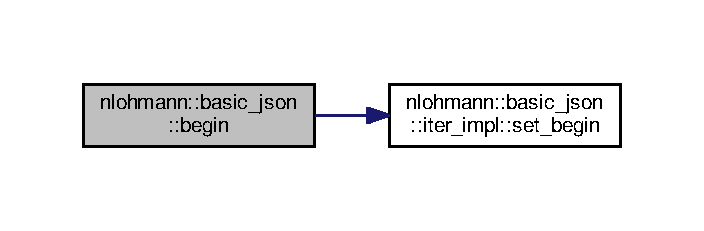
\includegraphics[width=338pt]{classnlohmann_1_1basic__json_a0ff28dac23f2bdecee9564d07f51dcdc_cgraph}
\end{center}
\end{figure}
\mbox{\Hypertarget{classnlohmann_1_1basic__json_a4f0f5dd42b2987ff20306ed78bd31d1d}\label{classnlohmann_1_1basic__json_a4f0f5dd42b2987ff20306ed78bd31d1d}} 
\index{nlohmann\+::basic\+\_\+json@{nlohmann\+::basic\+\_\+json}!begin@{begin}}
\index{begin@{begin}!nlohmann\+::basic\+\_\+json@{nlohmann\+::basic\+\_\+json}}
\subsubsection{\texorpdfstring{begin()}{begin()}\hspace{0.1cm}{\footnotesize\ttfamily [2/2]}}
{\footnotesize\ttfamily template$<$template$<$ typename U, typename V, typename... Args $>$ class Object\+Type = std\+::map, template$<$ typename U, typename... Args $>$ class Array\+Type = std\+::vector, class String\+Type  = std\+::string, class Boolean\+Type  = bool, class Number\+Integer\+Type  = std\+::int64\+\_\+t, class Number\+Unsigned\+Type  = std\+::uint64\+\_\+t, class Number\+Float\+Type  = double, template$<$ typename U $>$ class Allocator\+Type = std\+::allocator, template$<$ typename T, typename S\+F\+I\+N\+A\+E=void $>$ class J\+S\+O\+N\+Serializer = adl\+\_\+serializer$>$ \\
\hyperlink{classnlohmann_1_1basic__json_a41a70cf9993951836d129bb1c2b3126a}{const\+\_\+iterator} \hyperlink{classnlohmann_1_1basic__json}{nlohmann\+::basic\+\_\+json}$<$ Object\+Type, Array\+Type, String\+Type, Boolean\+Type, Number\+Integer\+Type, Number\+Unsigned\+Type, Number\+Float\+Type, Allocator\+Type, J\+S\+O\+N\+Serializer $>$\+::begin (\begin{DoxyParamCaption}{ }\end{DoxyParamCaption}) const\hspace{0.3cm}{\ttfamily [inline]}, {\ttfamily [noexcept]}}



returns a const iterator to the first element 

Returns a const iterator to the first element.

 \begin{DoxyReturn}{Returns}
const iterator to the first element
\end{DoxyReturn}
Constant.

This function helps {\ttfamily \hyperlink{classnlohmann_1_1basic__json}{basic\+\_\+json}} satisfying the \href{http://en.cppreference.com/w/cpp/concept/Container}{\tt Container} requirements\+:
\begin{DoxyItemize}
\item The complexity is constant.
\item Has the semantics of {\ttfamily const\+\_\+cast$<$const \hyperlink{classnlohmann_1_1basic__json}{basic\+\_\+json}\&$>$($\ast$this).\hyperlink{classnlohmann_1_1basic__json_a0ff28dac23f2bdecee9564d07f51dcdc}{begin()}}.
\end{DoxyItemize}

\{The following code shows an example for {\ttfamily \hyperlink{classnlohmann_1_1basic__json_ad865d6c291b237ae508d5cb2146b5877}{cbegin()}}.,cbegin\}

\begin{DoxySeeAlso}{See also}
\hyperlink{classnlohmann_1_1basic__json_a0ff28dac23f2bdecee9564d07f51dcdc}{begin()} -- returns an \hyperlink{classnlohmann_1_1basic__json_a099316232c76c034030a38faa6e34dca}{iterator} to the beginning 

\hyperlink{classnlohmann_1_1basic__json_a13e032a02a7fd8a93fdddc2fcbc4763c}{end()} -- returns an \hyperlink{classnlohmann_1_1basic__json_a099316232c76c034030a38faa6e34dca}{iterator} to the \hyperlink{classnlohmann_1_1basic__json_a13e032a02a7fd8a93fdddc2fcbc4763c}{end} 

\hyperlink{classnlohmann_1_1basic__json_a8dba7b7d2f38e6b0c614030aa43983f6}{cend()} -- returns a const \hyperlink{classnlohmann_1_1basic__json_a099316232c76c034030a38faa6e34dca}{iterator} to the \hyperlink{classnlohmann_1_1basic__json_a13e032a02a7fd8a93fdddc2fcbc4763c}{end}
\end{DoxySeeAlso}
\begin{DoxySince}{Since}
version 1.\+0.\+0 
\end{DoxySince}
\mbox{\Hypertarget{classnlohmann_1_1basic__json_ad865d6c291b237ae508d5cb2146b5877}\label{classnlohmann_1_1basic__json_ad865d6c291b237ae508d5cb2146b5877}} 
\index{nlohmann\+::basic\+\_\+json@{nlohmann\+::basic\+\_\+json}!cbegin@{cbegin}}
\index{cbegin@{cbegin}!nlohmann\+::basic\+\_\+json@{nlohmann\+::basic\+\_\+json}}
\subsubsection{\texorpdfstring{cbegin()}{cbegin()}}
{\footnotesize\ttfamily template$<$template$<$ typename U, typename V, typename... Args $>$ class Object\+Type = std\+::map, template$<$ typename U, typename... Args $>$ class Array\+Type = std\+::vector, class String\+Type  = std\+::string, class Boolean\+Type  = bool, class Number\+Integer\+Type  = std\+::int64\+\_\+t, class Number\+Unsigned\+Type  = std\+::uint64\+\_\+t, class Number\+Float\+Type  = double, template$<$ typename U $>$ class Allocator\+Type = std\+::allocator, template$<$ typename T, typename S\+F\+I\+N\+A\+E=void $>$ class J\+S\+O\+N\+Serializer = adl\+\_\+serializer$>$ \\
\hyperlink{classnlohmann_1_1basic__json_a41a70cf9993951836d129bb1c2b3126a}{const\+\_\+iterator} \hyperlink{classnlohmann_1_1basic__json}{nlohmann\+::basic\+\_\+json}$<$ Object\+Type, Array\+Type, String\+Type, Boolean\+Type, Number\+Integer\+Type, Number\+Unsigned\+Type, Number\+Float\+Type, Allocator\+Type, J\+S\+O\+N\+Serializer $>$\+::cbegin (\begin{DoxyParamCaption}{ }\end{DoxyParamCaption}) const\hspace{0.3cm}{\ttfamily [inline]}, {\ttfamily [noexcept]}}



returns a const iterator to the first element 

Returns a const iterator to the first element.

 \begin{DoxyReturn}{Returns}
const iterator to the first element
\end{DoxyReturn}
Constant.

This function helps {\ttfamily \hyperlink{classnlohmann_1_1basic__json}{basic\+\_\+json}} satisfying the \href{http://en.cppreference.com/w/cpp/concept/Container}{\tt Container} requirements\+:
\begin{DoxyItemize}
\item The complexity is constant.
\item Has the semantics of {\ttfamily const\+\_\+cast$<$const \hyperlink{classnlohmann_1_1basic__json}{basic\+\_\+json}\&$>$($\ast$this).\hyperlink{classnlohmann_1_1basic__json_a0ff28dac23f2bdecee9564d07f51dcdc}{begin()}}.
\end{DoxyItemize}

\{The following code shows an example for {\ttfamily \hyperlink{classnlohmann_1_1basic__json_ad865d6c291b237ae508d5cb2146b5877}{cbegin()}}.,cbegin\}

\begin{DoxySeeAlso}{See also}
\hyperlink{classnlohmann_1_1basic__json_a0ff28dac23f2bdecee9564d07f51dcdc}{begin()} -- returns an \hyperlink{classnlohmann_1_1basic__json_a099316232c76c034030a38faa6e34dca}{iterator} to the beginning 

\hyperlink{classnlohmann_1_1basic__json_a13e032a02a7fd8a93fdddc2fcbc4763c}{end()} -- returns an \hyperlink{classnlohmann_1_1basic__json_a099316232c76c034030a38faa6e34dca}{iterator} to the \hyperlink{classnlohmann_1_1basic__json_a13e032a02a7fd8a93fdddc2fcbc4763c}{end} 

\hyperlink{classnlohmann_1_1basic__json_a8dba7b7d2f38e6b0c614030aa43983f6}{cend()} -- returns a const \hyperlink{classnlohmann_1_1basic__json_a099316232c76c034030a38faa6e34dca}{iterator} to the \hyperlink{classnlohmann_1_1basic__json_a13e032a02a7fd8a93fdddc2fcbc4763c}{end}
\end{DoxySeeAlso}
\begin{DoxySince}{Since}
version 1.\+0.\+0 
\end{DoxySince}
Here is the call graph for this function\+:\nopagebreak
\begin{figure}[H]
\begin{center}
\leavevmode
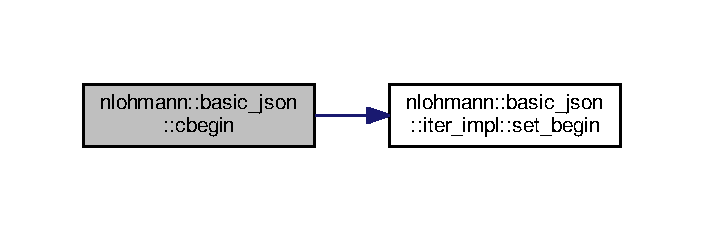
\includegraphics[width=338pt]{classnlohmann_1_1basic__json_ad865d6c291b237ae508d5cb2146b5877_cgraph}
\end{center}
\end{figure}
\mbox{\Hypertarget{classnlohmann_1_1basic__json_a8dba7b7d2f38e6b0c614030aa43983f6}\label{classnlohmann_1_1basic__json_a8dba7b7d2f38e6b0c614030aa43983f6}} 
\index{nlohmann\+::basic\+\_\+json@{nlohmann\+::basic\+\_\+json}!cend@{cend}}
\index{cend@{cend}!nlohmann\+::basic\+\_\+json@{nlohmann\+::basic\+\_\+json}}
\subsubsection{\texorpdfstring{cend()}{cend()}}
{\footnotesize\ttfamily template$<$template$<$ typename U, typename V, typename... Args $>$ class Object\+Type = std\+::map, template$<$ typename U, typename... Args $>$ class Array\+Type = std\+::vector, class String\+Type  = std\+::string, class Boolean\+Type  = bool, class Number\+Integer\+Type  = std\+::int64\+\_\+t, class Number\+Unsigned\+Type  = std\+::uint64\+\_\+t, class Number\+Float\+Type  = double, template$<$ typename U $>$ class Allocator\+Type = std\+::allocator, template$<$ typename T, typename S\+F\+I\+N\+A\+E=void $>$ class J\+S\+O\+N\+Serializer = adl\+\_\+serializer$>$ \\
\hyperlink{classnlohmann_1_1basic__json_a41a70cf9993951836d129bb1c2b3126a}{const\+\_\+iterator} \hyperlink{classnlohmann_1_1basic__json}{nlohmann\+::basic\+\_\+json}$<$ Object\+Type, Array\+Type, String\+Type, Boolean\+Type, Number\+Integer\+Type, Number\+Unsigned\+Type, Number\+Float\+Type, Allocator\+Type, J\+S\+O\+N\+Serializer $>$\+::cend (\begin{DoxyParamCaption}{ }\end{DoxyParamCaption}) const\hspace{0.3cm}{\ttfamily [inline]}, {\ttfamily [noexcept]}}



returns a const iterator to one past the last element 

Returns a const iterator to one past the last element.

 \begin{DoxyReturn}{Returns}
const iterator one past the last element
\end{DoxyReturn}
Constant.

This function helps {\ttfamily \hyperlink{classnlohmann_1_1basic__json}{basic\+\_\+json}} satisfying the \href{http://en.cppreference.com/w/cpp/concept/Container}{\tt Container} requirements\+:
\begin{DoxyItemize}
\item The complexity is constant.
\item Has the semantics of {\ttfamily const\+\_\+cast$<$const \hyperlink{classnlohmann_1_1basic__json}{basic\+\_\+json}\&$>$($\ast$this).\hyperlink{classnlohmann_1_1basic__json_a13e032a02a7fd8a93fdddc2fcbc4763c}{end()}}.
\end{DoxyItemize}

\{The following code shows an example for {\ttfamily \hyperlink{classnlohmann_1_1basic__json_a8dba7b7d2f38e6b0c614030aa43983f6}{cend()}}.,cend\}

\begin{DoxySeeAlso}{See also}
\hyperlink{classnlohmann_1_1basic__json_a13e032a02a7fd8a93fdddc2fcbc4763c}{end()} -- returns an \hyperlink{classnlohmann_1_1basic__json_a099316232c76c034030a38faa6e34dca}{iterator} to the \hyperlink{classnlohmann_1_1basic__json_a13e032a02a7fd8a93fdddc2fcbc4763c}{end} 

\hyperlink{classnlohmann_1_1basic__json_a0ff28dac23f2bdecee9564d07f51dcdc}{begin()} -- returns an \hyperlink{classnlohmann_1_1basic__json_a099316232c76c034030a38faa6e34dca}{iterator} to the beginning 

\hyperlink{classnlohmann_1_1basic__json_ad865d6c291b237ae508d5cb2146b5877}{cbegin()} -- returns a const \hyperlink{classnlohmann_1_1basic__json_a099316232c76c034030a38faa6e34dca}{iterator} to the beginning
\end{DoxySeeAlso}
\begin{DoxySince}{Since}
version 1.\+0.\+0 
\end{DoxySince}
Here is the call graph for this function\+:\nopagebreak
\begin{figure}[H]
\begin{center}
\leavevmode
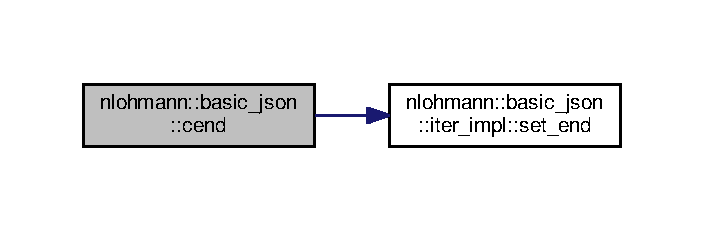
\includegraphics[width=338pt]{classnlohmann_1_1basic__json_a8dba7b7d2f38e6b0c614030aa43983f6_cgraph}
\end{center}
\end{figure}
\mbox{\Hypertarget{classnlohmann_1_1basic__json_a45e66a3b5e0696e5a984bd4c5a8df7a7}\label{classnlohmann_1_1basic__json_a45e66a3b5e0696e5a984bd4c5a8df7a7}} 
\index{nlohmann\+::basic\+\_\+json@{nlohmann\+::basic\+\_\+json}!check\+\_\+length@{check\+\_\+length}}
\index{check\+\_\+length@{check\+\_\+length}!nlohmann\+::basic\+\_\+json@{nlohmann\+::basic\+\_\+json}}
\subsubsection{\texorpdfstring{check\+\_\+length()}{check\_length()}}
{\footnotesize\ttfamily template$<$template$<$ typename U, typename V, typename... Args $>$ class Object\+Type = std\+::map, template$<$ typename U, typename... Args $>$ class Array\+Type = std\+::vector, class String\+Type  = std\+::string, class Boolean\+Type  = bool, class Number\+Integer\+Type  = std\+::int64\+\_\+t, class Number\+Unsigned\+Type  = std\+::uint64\+\_\+t, class Number\+Float\+Type  = double, template$<$ typename U $>$ class Allocator\+Type = std\+::allocator, template$<$ typename T, typename S\+F\+I\+N\+A\+E=void $>$ class J\+S\+O\+N\+Serializer = adl\+\_\+serializer$>$ \\
static void \hyperlink{classnlohmann_1_1basic__json}{nlohmann\+::basic\+\_\+json}$<$ Object\+Type, Array\+Type, String\+Type, Boolean\+Type, Number\+Integer\+Type, Number\+Unsigned\+Type, Number\+Float\+Type, Allocator\+Type, J\+S\+O\+N\+Serializer $>$\+::check\+\_\+length (\begin{DoxyParamCaption}\item[{const size\+\_\+t}]{size,  }\item[{const size\+\_\+t}]{len,  }\item[{const size\+\_\+t}]{offset }\end{DoxyParamCaption})\hspace{0.3cm}{\ttfamily [inline]}, {\ttfamily [static]}, {\ttfamily [private]}}

\mbox{\Hypertarget{classnlohmann_1_1basic__json_abfeba47810ca72f2176419942c4e1952}\label{classnlohmann_1_1basic__json_abfeba47810ca72f2176419942c4e1952}} 
\index{nlohmann\+::basic\+\_\+json@{nlohmann\+::basic\+\_\+json}!clear@{clear}}
\index{clear@{clear}!nlohmann\+::basic\+\_\+json@{nlohmann\+::basic\+\_\+json}}
\subsubsection{\texorpdfstring{clear()}{clear()}}
{\footnotesize\ttfamily template$<$template$<$ typename U, typename V, typename... Args $>$ class Object\+Type = std\+::map, template$<$ typename U, typename... Args $>$ class Array\+Type = std\+::vector, class String\+Type  = std\+::string, class Boolean\+Type  = bool, class Number\+Integer\+Type  = std\+::int64\+\_\+t, class Number\+Unsigned\+Type  = std\+::uint64\+\_\+t, class Number\+Float\+Type  = double, template$<$ typename U $>$ class Allocator\+Type = std\+::allocator, template$<$ typename T, typename S\+F\+I\+N\+A\+E=void $>$ class J\+S\+O\+N\+Serializer = adl\+\_\+serializer$>$ \\
void \hyperlink{classnlohmann_1_1basic__json}{nlohmann\+::basic\+\_\+json}$<$ Object\+Type, Array\+Type, String\+Type, Boolean\+Type, Number\+Integer\+Type, Number\+Unsigned\+Type, Number\+Float\+Type, Allocator\+Type, J\+S\+O\+N\+Serializer $>$\+::clear (\begin{DoxyParamCaption}{ }\end{DoxyParamCaption})\hspace{0.3cm}{\ttfamily [inline]}, {\ttfamily [noexcept]}}



clears the contents 

Clears the content of a J\+S\+ON value and resets it to the default value as if \hyperlink{classnlohmann_1_1basic__json_a32124a16dc80729d964d9caf607c2bc8}{basic\+\_\+json(value\+\_\+t)} would have been called\+:

\tabulinesep=1mm
\begin{longtabu} spread 0pt [c]{*{2}{|X[-1]}|}
\hline
\rowcolor{\tableheadbgcolor}\textbf{ Value type }&\textbf{ initial value  }\\\cline{1-2}
\endfirsthead
\hline
\endfoot
\hline
\rowcolor{\tableheadbgcolor}\textbf{ Value type }&\textbf{ initial value  }\\\cline{1-2}
\endhead
null &{\ttfamily null} \\\cline{1-2}
boolean &{\ttfamily false} \\\cline{1-2}
string &{\ttfamily \char`\"{}\char`\"{}} \\\cline{1-2}
number &{\ttfamily 0} \\\cline{1-2}
object &{\ttfamily \{\}} \\\cline{1-2}
array &{\ttfamily \mbox{[}\mbox{]}} \\\cline{1-2}
\end{longtabu}
Linear in the size of the J\+S\+ON value.

\{The example below shows the effect of {\ttfamily \hyperlink{classnlohmann_1_1basic__json_abfeba47810ca72f2176419942c4e1952}{clear()}} to different J\+S\+ON types.,clear\}

\begin{DoxySince}{Since}
version 1.\+0.\+0 
\end{DoxySince}
\mbox{\Hypertarget{classnlohmann_1_1basic__json_a5261eba9637f59d17d6cab5f14ce5747}\label{classnlohmann_1_1basic__json_a5261eba9637f59d17d6cab5f14ce5747}} 
\index{nlohmann\+::basic\+\_\+json@{nlohmann\+::basic\+\_\+json}!count@{count}}
\index{count@{count}!nlohmann\+::basic\+\_\+json@{nlohmann\+::basic\+\_\+json}}
\subsubsection{\texorpdfstring{count()}{count()}}
{\footnotesize\ttfamily template$<$template$<$ typename U, typename V, typename... Args $>$ class Object\+Type = std\+::map, template$<$ typename U, typename... Args $>$ class Array\+Type = std\+::vector, class String\+Type  = std\+::string, class Boolean\+Type  = bool, class Number\+Integer\+Type  = std\+::int64\+\_\+t, class Number\+Unsigned\+Type  = std\+::uint64\+\_\+t, class Number\+Float\+Type  = double, template$<$ typename U $>$ class Allocator\+Type = std\+::allocator, template$<$ typename T, typename S\+F\+I\+N\+A\+E=void $>$ class J\+S\+O\+N\+Serializer = adl\+\_\+serializer$>$ \\
\hyperlink{classnlohmann_1_1basic__json_a39f2cd0b58106097e0e67bf185cc519b}{size\+\_\+type} \hyperlink{classnlohmann_1_1basic__json}{nlohmann\+::basic\+\_\+json}$<$ Object\+Type, Array\+Type, String\+Type, Boolean\+Type, Number\+Integer\+Type, Number\+Unsigned\+Type, Number\+Float\+Type, Allocator\+Type, J\+S\+O\+N\+Serializer $>$\+::count (\begin{DoxyParamCaption}\item[{typename object\+\_\+t\+::key\+\_\+type}]{key }\end{DoxyParamCaption}) const\hspace{0.3cm}{\ttfamily [inline]}}



returns the number of occurrences of a key in a J\+S\+ON object 

Returns the number of elements with key {\itshape key}. If Object\+Type is the default {\ttfamily std\+::map} type, the return value will always be {\ttfamily 0} ({\itshape key} was not found) or {\ttfamily 1} ({\itshape key} was found).

\begin{DoxyNote}{Note}
This method always returns {\ttfamily 0} when executed on a J\+S\+ON type that is not an object.
\end{DoxyNote}

\begin{DoxyParams}[1]{Parameters}
\mbox{\tt in}  & {\em key} & key value of the element to count\\
\hline
\end{DoxyParams}
\begin{DoxyReturn}{Returns}
Number of elements with key {\itshape key}. If the J\+S\+ON value is not an object, the return value will be {\ttfamily 0}.
\end{DoxyReturn}
Logarithmic in the size of the J\+S\+ON object.

\{The example shows how {\ttfamily \hyperlink{classnlohmann_1_1basic__json_a5261eba9637f59d17d6cab5f14ce5747}{count()}} is used.,count\}

\begin{DoxySince}{Since}
version 1.\+0.\+0 
\end{DoxySince}
\mbox{\Hypertarget{classnlohmann_1_1basic__json_a1e0769d22d54573f294da0e5c6abc9de}\label{classnlohmann_1_1basic__json_a1e0769d22d54573f294da0e5c6abc9de}} 
\index{nlohmann\+::basic\+\_\+json@{nlohmann\+::basic\+\_\+json}!crbegin@{crbegin}}
\index{crbegin@{crbegin}!nlohmann\+::basic\+\_\+json@{nlohmann\+::basic\+\_\+json}}
\subsubsection{\texorpdfstring{crbegin()}{crbegin()}}
{\footnotesize\ttfamily template$<$template$<$ typename U, typename V, typename... Args $>$ class Object\+Type = std\+::map, template$<$ typename U, typename... Args $>$ class Array\+Type = std\+::vector, class String\+Type  = std\+::string, class Boolean\+Type  = bool, class Number\+Integer\+Type  = std\+::int64\+\_\+t, class Number\+Unsigned\+Type  = std\+::uint64\+\_\+t, class Number\+Float\+Type  = double, template$<$ typename U $>$ class Allocator\+Type = std\+::allocator, template$<$ typename T, typename S\+F\+I\+N\+A\+E=void $>$ class J\+S\+O\+N\+Serializer = adl\+\_\+serializer$>$ \\
\hyperlink{classnlohmann_1_1basic__json_a72be3c24bfa24f0993d6c11af03e7404}{const\+\_\+reverse\+\_\+iterator} \hyperlink{classnlohmann_1_1basic__json}{nlohmann\+::basic\+\_\+json}$<$ Object\+Type, Array\+Type, String\+Type, Boolean\+Type, Number\+Integer\+Type, Number\+Unsigned\+Type, Number\+Float\+Type, Allocator\+Type, J\+S\+O\+N\+Serializer $>$\+::crbegin (\begin{DoxyParamCaption}{ }\end{DoxyParamCaption}) const\hspace{0.3cm}{\ttfamily [inline]}, {\ttfamily [noexcept]}}



returns a const reverse iterator to the last element 

Returns a const iterator to the reverse-\/beginning; that is, the last element.

  Constant.

This function helps {\ttfamily \hyperlink{classnlohmann_1_1basic__json}{basic\+\_\+json}} satisfying the \href{http://en.cppreference.com/w/cpp/concept/ReversibleContainer}{\tt Reversible\+Container} requirements\+:
\begin{DoxyItemize}
\item The complexity is constant.
\item Has the semantics of {\ttfamily const\+\_\+cast$<$const \hyperlink{classnlohmann_1_1basic__json}{basic\+\_\+json}\&$>$($\ast$this).\hyperlink{classnlohmann_1_1basic__json_a1ef93e2006dbe52667294f5ef38b0b10}{rbegin()}}.
\end{DoxyItemize}

\{The following code shows an example for {\ttfamily \hyperlink{classnlohmann_1_1basic__json_a1e0769d22d54573f294da0e5c6abc9de}{crbegin()}}.,crbegin\}

\begin{DoxySeeAlso}{See also}
\hyperlink{classnlohmann_1_1basic__json_a1ef93e2006dbe52667294f5ef38b0b10}{rbegin()} -- returns a reverse \hyperlink{classnlohmann_1_1basic__json_a099316232c76c034030a38faa6e34dca}{iterator} to the beginning 

\hyperlink{classnlohmann_1_1basic__json_ac77aed0925d447744676725ab0b6d535}{rend()} -- returns a reverse \hyperlink{classnlohmann_1_1basic__json_a099316232c76c034030a38faa6e34dca}{iterator} to the \hyperlink{classnlohmann_1_1basic__json_a13e032a02a7fd8a93fdddc2fcbc4763c}{end} 

\hyperlink{classnlohmann_1_1basic__json_a5795b029dbf28e0cb2c7a439ec5d0a88}{crend()} -- returns a const reverse \hyperlink{classnlohmann_1_1basic__json_a099316232c76c034030a38faa6e34dca}{iterator} to the \hyperlink{classnlohmann_1_1basic__json_a13e032a02a7fd8a93fdddc2fcbc4763c}{end}
\end{DoxySeeAlso}
\begin{DoxySince}{Since}
version 1.\+0.\+0 
\end{DoxySince}
\mbox{\Hypertarget{classnlohmann_1_1basic__json_a81100399cf3e2be457937be7db3f5729}\label{classnlohmann_1_1basic__json_a81100399cf3e2be457937be7db3f5729}} 
\index{nlohmann\+::basic\+\_\+json@{nlohmann\+::basic\+\_\+json}!create@{create}}
\index{create@{create}!nlohmann\+::basic\+\_\+json@{nlohmann\+::basic\+\_\+json}}
\subsubsection{\texorpdfstring{create()}{create()}}
{\footnotesize\ttfamily template$<$template$<$ typename U, typename V, typename... Args $>$ class Object\+Type = std\+::map, template$<$ typename U, typename... Args $>$ class Array\+Type = std\+::vector, class String\+Type  = std\+::string, class Boolean\+Type  = bool, class Number\+Integer\+Type  = std\+::int64\+\_\+t, class Number\+Unsigned\+Type  = std\+::uint64\+\_\+t, class Number\+Float\+Type  = double, template$<$ typename U $>$ class Allocator\+Type = std\+::allocator, template$<$ typename T, typename S\+F\+I\+N\+A\+E=void $>$ class J\+S\+O\+N\+Serializer = adl\+\_\+serializer$>$ \\
template$<$typename T , typename... Args$>$ \\
static T$\ast$ \hyperlink{classnlohmann_1_1basic__json}{nlohmann\+::basic\+\_\+json}$<$ Object\+Type, Array\+Type, String\+Type, Boolean\+Type, Number\+Integer\+Type, Number\+Unsigned\+Type, Number\+Float\+Type, Allocator\+Type, J\+S\+O\+N\+Serializer $>$\+::create (\begin{DoxyParamCaption}\item[{Args \&\&...}]{args }\end{DoxyParamCaption})\hspace{0.3cm}{\ttfamily [inline]}, {\ttfamily [static]}, {\ttfamily [private]}}



helper for exception-\/safe object creation 

\mbox{\Hypertarget{classnlohmann_1_1basic__json_a5795b029dbf28e0cb2c7a439ec5d0a88}\label{classnlohmann_1_1basic__json_a5795b029dbf28e0cb2c7a439ec5d0a88}} 
\index{nlohmann\+::basic\+\_\+json@{nlohmann\+::basic\+\_\+json}!crend@{crend}}
\index{crend@{crend}!nlohmann\+::basic\+\_\+json@{nlohmann\+::basic\+\_\+json}}
\subsubsection{\texorpdfstring{crend()}{crend()}}
{\footnotesize\ttfamily template$<$template$<$ typename U, typename V, typename... Args $>$ class Object\+Type = std\+::map, template$<$ typename U, typename... Args $>$ class Array\+Type = std\+::vector, class String\+Type  = std\+::string, class Boolean\+Type  = bool, class Number\+Integer\+Type  = std\+::int64\+\_\+t, class Number\+Unsigned\+Type  = std\+::uint64\+\_\+t, class Number\+Float\+Type  = double, template$<$ typename U $>$ class Allocator\+Type = std\+::allocator, template$<$ typename T, typename S\+F\+I\+N\+A\+E=void $>$ class J\+S\+O\+N\+Serializer = adl\+\_\+serializer$>$ \\
\hyperlink{classnlohmann_1_1basic__json_a72be3c24bfa24f0993d6c11af03e7404}{const\+\_\+reverse\+\_\+iterator} \hyperlink{classnlohmann_1_1basic__json}{nlohmann\+::basic\+\_\+json}$<$ Object\+Type, Array\+Type, String\+Type, Boolean\+Type, Number\+Integer\+Type, Number\+Unsigned\+Type, Number\+Float\+Type, Allocator\+Type, J\+S\+O\+N\+Serializer $>$\+::crend (\begin{DoxyParamCaption}{ }\end{DoxyParamCaption}) const\hspace{0.3cm}{\ttfamily [inline]}, {\ttfamily [noexcept]}}



returns a const reverse iterator to one before the first 

Returns a const reverse iterator to the reverse-\/end; that is, one before the first element.

  Constant.

This function helps {\ttfamily \hyperlink{classnlohmann_1_1basic__json}{basic\+\_\+json}} satisfying the \href{http://en.cppreference.com/w/cpp/concept/ReversibleContainer}{\tt Reversible\+Container} requirements\+:
\begin{DoxyItemize}
\item The complexity is constant.
\item Has the semantics of {\ttfamily const\+\_\+cast$<$const \hyperlink{classnlohmann_1_1basic__json}{basic\+\_\+json}\&$>$($\ast$this).\hyperlink{classnlohmann_1_1basic__json_ac77aed0925d447744676725ab0b6d535}{rend()}}.
\end{DoxyItemize}

\{The following code shows an example for {\ttfamily \hyperlink{classnlohmann_1_1basic__json_a5795b029dbf28e0cb2c7a439ec5d0a88}{crend()}}.,crend\}

\begin{DoxySeeAlso}{See also}
\hyperlink{classnlohmann_1_1basic__json_ac77aed0925d447744676725ab0b6d535}{rend()} -- returns a reverse \hyperlink{classnlohmann_1_1basic__json_a099316232c76c034030a38faa6e34dca}{iterator} to the \hyperlink{classnlohmann_1_1basic__json_a13e032a02a7fd8a93fdddc2fcbc4763c}{end} 

\hyperlink{classnlohmann_1_1basic__json_a1ef93e2006dbe52667294f5ef38b0b10}{rbegin()} -- returns a reverse \hyperlink{classnlohmann_1_1basic__json_a099316232c76c034030a38faa6e34dca}{iterator} to the beginning 

\hyperlink{classnlohmann_1_1basic__json_a1e0769d22d54573f294da0e5c6abc9de}{crbegin()} -- returns a const reverse \hyperlink{classnlohmann_1_1basic__json_a099316232c76c034030a38faa6e34dca}{iterator} to the beginning
\end{DoxySeeAlso}
\begin{DoxySince}{Since}
version 1.\+0.\+0 
\end{DoxySince}
\mbox{\Hypertarget{classnlohmann_1_1basic__json_a543bd5f7490de54c875b2c0912dc9a49}\label{classnlohmann_1_1basic__json_a543bd5f7490de54c875b2c0912dc9a49}} 
\index{nlohmann\+::basic\+\_\+json@{nlohmann\+::basic\+\_\+json}!diff@{diff}}
\index{diff@{diff}!nlohmann\+::basic\+\_\+json@{nlohmann\+::basic\+\_\+json}}
\subsubsection{\texorpdfstring{diff()}{diff()}}
{\footnotesize\ttfamily template$<$template$<$ typename U, typename V, typename... Args $>$ class Object\+Type = std\+::map, template$<$ typename U, typename... Args $>$ class Array\+Type = std\+::vector, class String\+Type  = std\+::string, class Boolean\+Type  = bool, class Number\+Integer\+Type  = std\+::int64\+\_\+t, class Number\+Unsigned\+Type  = std\+::uint64\+\_\+t, class Number\+Float\+Type  = double, template$<$ typename U $>$ class Allocator\+Type = std\+::allocator, template$<$ typename T, typename S\+F\+I\+N\+A\+E=void $>$ class J\+S\+O\+N\+Serializer = adl\+\_\+serializer$>$ \\
static \hyperlink{classnlohmann_1_1basic__json}{basic\+\_\+json} \hyperlink{classnlohmann_1_1basic__json}{nlohmann\+::basic\+\_\+json}$<$ Object\+Type, Array\+Type, String\+Type, Boolean\+Type, Number\+Integer\+Type, Number\+Unsigned\+Type, Number\+Float\+Type, Allocator\+Type, J\+S\+O\+N\+Serializer $>$\+::diff (\begin{DoxyParamCaption}\item[{const \hyperlink{classnlohmann_1_1basic__json}{basic\+\_\+json}$<$ Object\+Type, Array\+Type, String\+Type, Boolean\+Type, Number\+Integer\+Type, Number\+Unsigned\+Type, Number\+Float\+Type, Allocator\+Type, J\+S\+O\+N\+Serializer $>$ \&}]{source,  }\item[{const \hyperlink{classnlohmann_1_1basic__json}{basic\+\_\+json}$<$ Object\+Type, Array\+Type, String\+Type, Boolean\+Type, Number\+Integer\+Type, Number\+Unsigned\+Type, Number\+Float\+Type, Allocator\+Type, J\+S\+O\+N\+Serializer $>$ \&}]{target,  }\item[{const std\+::string \&}]{path = {\ttfamily \char`\"{}\char`\"{}} }\end{DoxyParamCaption})\hspace{0.3cm}{\ttfamily [inline]}, {\ttfamily [static]}}



creates a diff as a J\+S\+ON patch 

Creates a \href{http://jsonpatch.com}{\tt J\+S\+ON Patch} so that value {\itshape source} can be changed into the value {\itshape target} by calling \hyperlink{classnlohmann_1_1basic__json_a81e0c41a4a9dff4df2f6973f7f8b2a83}{patch} function.

\begin{DoxyInvariant}{Invariant}
For two J\+S\+ON values {\itshape source} and {\itshape target}, the following code yields always {\ttfamily true}\+: 
\begin{DoxyCode}
source.patch(\hyperlink{classnlohmann_1_1basic__json_a543bd5f7490de54c875b2c0912dc9a49}{diff}(source, target)) == target;
\end{DoxyCode}

\end{DoxyInvariant}
\begin{DoxyNote}{Note}
Currently, only {\ttfamily remove}, {\ttfamily add}, and {\ttfamily replace} operations are generated.
\end{DoxyNote}

\begin{DoxyParams}[1]{Parameters}
\mbox{\tt in}  & {\em source} & J\+S\+ON value to compare from \\
\hline
\mbox{\tt in}  & {\em target} & J\+S\+ON value to compare against \\
\hline
\mbox{\tt in}  & {\em path} & helper value to create J\+S\+ON pointers\\
\hline
\end{DoxyParams}
\begin{DoxyReturn}{Returns}
a J\+S\+ON patch to convert the {\itshape source} to {\itshape target} 
\end{DoxyReturn}
Linear in the lengths of {\itshape source} and {\itshape target}.

\{The following code shows how a J\+S\+ON patch is created as a diff for two J\+S\+ON values.,diff\}

\begin{DoxySeeAlso}{See also}
\hyperlink{classnlohmann_1_1basic__json_a81e0c41a4a9dff4df2f6973f7f8b2a83}{patch} -- apply a J\+S\+ON \hyperlink{classnlohmann_1_1basic__json_a81e0c41a4a9dff4df2f6973f7f8b2a83}{patch}

\href{https://tools.ietf.org/html/rfc6902}{\tt R\+FC 6902 (J\+S\+ON Patch)}
\end{DoxySeeAlso}
\begin{DoxySince}{Since}
version 2.\+0.\+0 
\end{DoxySince}
Here is the call graph for this function\+:\nopagebreak
\begin{figure}[H]
\begin{center}
\leavevmode
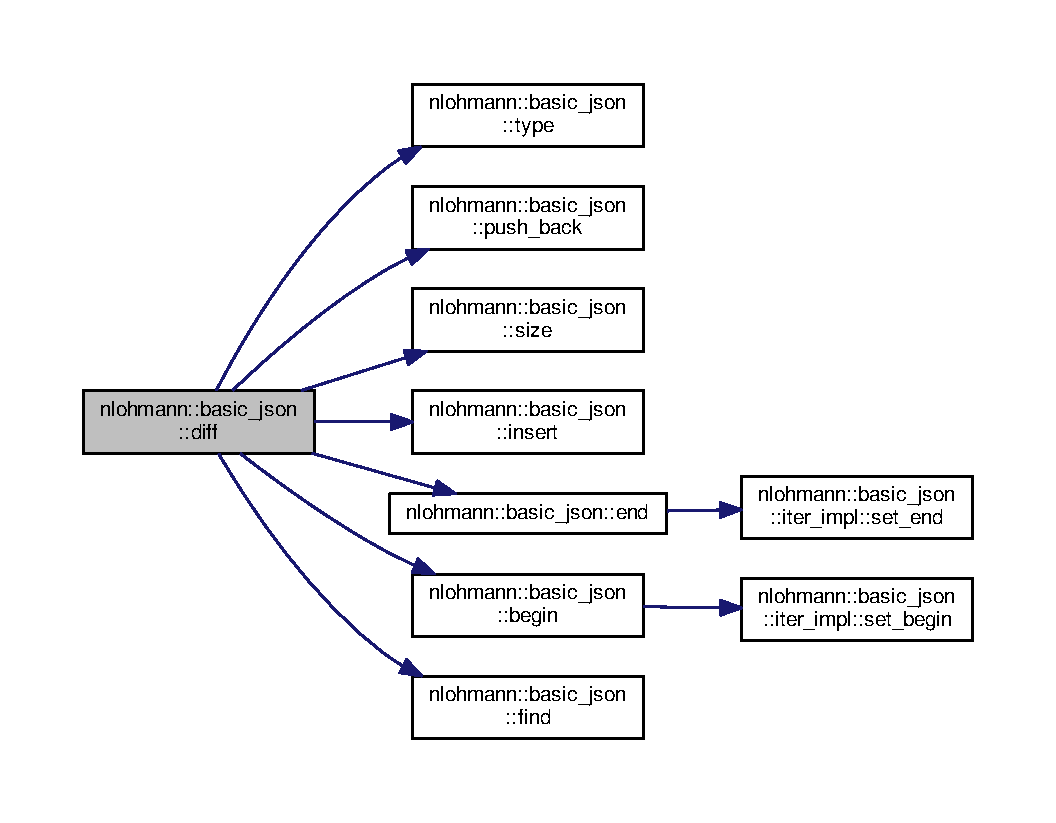
\includegraphics[width=350pt]{classnlohmann_1_1basic__json_a543bd5f7490de54c875b2c0912dc9a49_cgraph}
\end{center}
\end{figure}
\mbox{\Hypertarget{classnlohmann_1_1basic__json_a5319dc1bb9dfe19ce7ff559aaded3422}\label{classnlohmann_1_1basic__json_a5319dc1bb9dfe19ce7ff559aaded3422}} 
\index{nlohmann\+::basic\+\_\+json@{nlohmann\+::basic\+\_\+json}!dump@{dump}}
\index{dump@{dump}!nlohmann\+::basic\+\_\+json@{nlohmann\+::basic\+\_\+json}}
\subsubsection{\texorpdfstring{dump()}{dump()}\hspace{0.1cm}{\footnotesize\ttfamily [1/2]}}
{\footnotesize\ttfamily template$<$template$<$ typename U, typename V, typename... Args $>$ class Object\+Type = std\+::map, template$<$ typename U, typename... Args $>$ class Array\+Type = std\+::vector, class String\+Type  = std\+::string, class Boolean\+Type  = bool, class Number\+Integer\+Type  = std\+::int64\+\_\+t, class Number\+Unsigned\+Type  = std\+::uint64\+\_\+t, class Number\+Float\+Type  = double, template$<$ typename U $>$ class Allocator\+Type = std\+::allocator, template$<$ typename T, typename S\+F\+I\+N\+A\+E=void $>$ class J\+S\+O\+N\+Serializer = adl\+\_\+serializer$>$ \\
\hyperlink{classnlohmann_1_1basic__json_a61f8566a1a85a424c7266fb531dca005}{string\+\_\+t} \hyperlink{classnlohmann_1_1basic__json}{nlohmann\+::basic\+\_\+json}$<$ Object\+Type, Array\+Type, String\+Type, Boolean\+Type, Number\+Integer\+Type, Number\+Unsigned\+Type, Number\+Float\+Type, Allocator\+Type, J\+S\+O\+N\+Serializer $>$\+::dump (\begin{DoxyParamCaption}\item[{const int}]{indent = {\ttfamily -\/1} }\end{DoxyParamCaption}) const\hspace{0.3cm}{\ttfamily [inline]}}



serialization 

Serialization function for J\+S\+ON values. The function tries to mimic Python\textquotesingle{}s {\ttfamily json.\+dumps()} function, and currently supports its {\itshape indent} parameter.


\begin{DoxyParams}[1]{Parameters}
\mbox{\tt in}  & {\em indent} & If indent is nonnegative, then array elements and object members will be pretty-\/printed with that indent level. An indent level of {\ttfamily 0} will only insert newlines. {\ttfamily -\/1} (the default) selects the most compact representation.\\
\hline
\end{DoxyParams}
\begin{DoxyReturn}{Returns}
string containing the serialization of the J\+S\+ON value
\end{DoxyReturn}
Linear.

\{The following example shows the effect of different {\itshape indent} parameters to the result of the serialization.,dump\}

\begin{DoxySeeAlso}{See also}
\href{https://docs.python.org/2/library/json.html#json.dump}{\tt https\+://docs.\+python.\+org/2/library/json.\+html\#json.\+dump}
\end{DoxySeeAlso}
\begin{DoxySince}{Since}
version 1.\+0.\+0 
\end{DoxySince}
\mbox{\Hypertarget{classnlohmann_1_1basic__json_ade04010df46f1f247623b85191976239}\label{classnlohmann_1_1basic__json_ade04010df46f1f247623b85191976239}} 
\index{nlohmann\+::basic\+\_\+json@{nlohmann\+::basic\+\_\+json}!dump@{dump}}
\index{dump@{dump}!nlohmann\+::basic\+\_\+json@{nlohmann\+::basic\+\_\+json}}
\subsubsection{\texorpdfstring{dump()}{dump()}\hspace{0.1cm}{\footnotesize\ttfamily [2/2]}}
{\footnotesize\ttfamily template$<$template$<$ typename U, typename V, typename... Args $>$ class Object\+Type = std\+::map, template$<$ typename U, typename... Args $>$ class Array\+Type = std\+::vector, class String\+Type  = std\+::string, class Boolean\+Type  = bool, class Number\+Integer\+Type  = std\+::int64\+\_\+t, class Number\+Unsigned\+Type  = std\+::uint64\+\_\+t, class Number\+Float\+Type  = double, template$<$ typename U $>$ class Allocator\+Type = std\+::allocator, template$<$ typename T, typename S\+F\+I\+N\+A\+E=void $>$ class J\+S\+O\+N\+Serializer = adl\+\_\+serializer$>$ \\
void \hyperlink{classnlohmann_1_1basic__json}{nlohmann\+::basic\+\_\+json}$<$ Object\+Type, Array\+Type, String\+Type, Boolean\+Type, Number\+Integer\+Type, Number\+Unsigned\+Type, Number\+Float\+Type, Allocator\+Type, J\+S\+O\+N\+Serializer $>$\+::dump (\begin{DoxyParamCaption}\item[{std\+::ostream \&}]{o,  }\item[{const bool}]{pretty\+\_\+print,  }\item[{const unsigned int}]{indent\+\_\+step,  }\item[{const unsigned int}]{current\+\_\+indent = {\ttfamily 0} }\end{DoxyParamCaption}) const\hspace{0.3cm}{\ttfamily [inline]}, {\ttfamily [private]}}



internal implementation of the serialization function 

This function is called by the public member function dump and organizes the serialization internally. The indentation level is propagated as additional parameter. In case of arrays and objects, the function is called recursively. Note that


\begin{DoxyItemize}
\item strings and object keys are escaped using {\ttfamily \hyperlink{classnlohmann_1_1basic__json_af6e1e06b6c274734ccb7de1ef770a915}{escape\+\_\+string()}}
\item integer numbers are converted implicitly via {\ttfamily operator$<$$<$}
\item floating-\/point numbers are converted to a string using {\ttfamily \char`\"{}\%g\char`\"{}} format
\end{DoxyItemize}


\begin{DoxyParams}[1]{Parameters}
\mbox{\tt out}  & {\em o} & stream to write to \\
\hline
\mbox{\tt in}  & {\em pretty\+\_\+print} & whether the output shall be pretty-\/printed \\
\hline
\mbox{\tt in}  & {\em indent\+\_\+step} & the indent level \\
\hline
\mbox{\tt in}  & {\em current\+\_\+indent} & the current indent level (only used internally) \\
\hline
\end{DoxyParams}
Here is the call graph for this function\+:\nopagebreak
\begin{figure}[H]
\begin{center}
\leavevmode
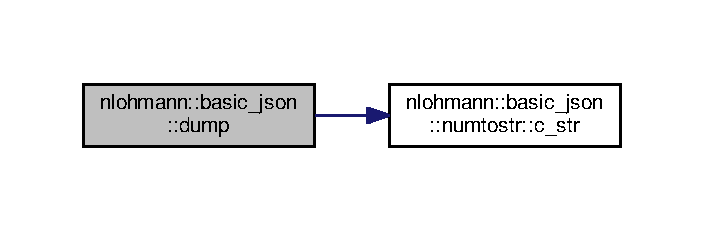
\includegraphics[width=338pt]{classnlohmann_1_1basic__json_ade04010df46f1f247623b85191976239_cgraph}
\end{center}
\end{figure}
\mbox{\Hypertarget{classnlohmann_1_1basic__json_a5338e282d1d02bed389d852dd670d98d}\label{classnlohmann_1_1basic__json_a5338e282d1d02bed389d852dd670d98d}} 
\index{nlohmann\+::basic\+\_\+json@{nlohmann\+::basic\+\_\+json}!emplace@{emplace}}
\index{emplace@{emplace}!nlohmann\+::basic\+\_\+json@{nlohmann\+::basic\+\_\+json}}
\subsubsection{\texorpdfstring{emplace()}{emplace()}}
{\footnotesize\ttfamily template$<$template$<$ typename U, typename V, typename... Args $>$ class Object\+Type = std\+::map, template$<$ typename U, typename... Args $>$ class Array\+Type = std\+::vector, class String\+Type  = std\+::string, class Boolean\+Type  = bool, class Number\+Integer\+Type  = std\+::int64\+\_\+t, class Number\+Unsigned\+Type  = std\+::uint64\+\_\+t, class Number\+Float\+Type  = double, template$<$ typename U $>$ class Allocator\+Type = std\+::allocator, template$<$ typename T, typename S\+F\+I\+N\+A\+E=void $>$ class J\+S\+O\+N\+Serializer = adl\+\_\+serializer$>$ \\
template$<$class... Args$>$ \\
std\+::pair$<$\hyperlink{classnlohmann_1_1basic__json_a099316232c76c034030a38faa6e34dca}{iterator}, bool$>$ \hyperlink{classnlohmann_1_1basic__json}{nlohmann\+::basic\+\_\+json}$<$ Object\+Type, Array\+Type, String\+Type, Boolean\+Type, Number\+Integer\+Type, Number\+Unsigned\+Type, Number\+Float\+Type, Allocator\+Type, J\+S\+O\+N\+Serializer $>$\+::emplace (\begin{DoxyParamCaption}\item[{Args \&\&...}]{args }\end{DoxyParamCaption})\hspace{0.3cm}{\ttfamily [inline]}}



add an object to an object if key does not exist 

Inserts a new element into a J\+S\+ON object constructed in-\/place with the given {\itshape args} if there is no element with the key in the container. If the function is called on a J\+S\+ON null value, an empty object is created before appending the value created from {\itshape args}.


\begin{DoxyParams}[1]{Parameters}
\mbox{\tt in}  & {\em args} & arguments to forward to a constructor of \hyperlink{classnlohmann_1_1basic__json}{basic\+\_\+json} \\
\hline
\end{DoxyParams}

\begin{DoxyTemplParams}{Template Parameters}
{\em Args} & compatible types to create a \hyperlink{classnlohmann_1_1basic__json}{basic\+\_\+json} object\\
\hline
\end{DoxyTemplParams}
\begin{DoxyReturn}{Returns}
a pair consisting of an iterator to the inserted element, or the already-\/existing element if no insertion happened, and a bool denoting whether the insertion took place.
\end{DoxyReturn}

\begin{DoxyExceptions}{Exceptions}
{\em std\+::domain\+\_\+error} & when called on a type other than J\+S\+ON object or null; example\+: {\ttfamily \char`\"{}cannot use emplace() with number\char`\"{}}\\
\hline
\end{DoxyExceptions}
Logarithmic in the size of the container, O(log({\ttfamily \hyperlink{classnlohmann_1_1basic__json_a25e27ad0c6d53c01871c5485e1f75b96}{size()}})).

\{The example shows how {\ttfamily \hyperlink{classnlohmann_1_1basic__json_a5338e282d1d02bed389d852dd670d98d}{emplace()}} can be used to add elements to a J\+S\+ON object. Note how the {\ttfamily null} value was silently converted to a J\+S\+ON object. Further note how no value is added if there was already one value stored with the same key.,emplace\}

\begin{DoxySince}{Since}
version 2.\+0.\+8 
\end{DoxySince}
\mbox{\Hypertarget{classnlohmann_1_1basic__json_aacf5eed15a8b66fb1e88910707a5e229}\label{classnlohmann_1_1basic__json_aacf5eed15a8b66fb1e88910707a5e229}} 
\index{nlohmann\+::basic\+\_\+json@{nlohmann\+::basic\+\_\+json}!emplace\+\_\+back@{emplace\+\_\+back}}
\index{emplace\+\_\+back@{emplace\+\_\+back}!nlohmann\+::basic\+\_\+json@{nlohmann\+::basic\+\_\+json}}
\subsubsection{\texorpdfstring{emplace\+\_\+back()}{emplace\_back()}}
{\footnotesize\ttfamily template$<$template$<$ typename U, typename V, typename... Args $>$ class Object\+Type = std\+::map, template$<$ typename U, typename... Args $>$ class Array\+Type = std\+::vector, class String\+Type  = std\+::string, class Boolean\+Type  = bool, class Number\+Integer\+Type  = std\+::int64\+\_\+t, class Number\+Unsigned\+Type  = std\+::uint64\+\_\+t, class Number\+Float\+Type  = double, template$<$ typename U $>$ class Allocator\+Type = std\+::allocator, template$<$ typename T, typename S\+F\+I\+N\+A\+E=void $>$ class J\+S\+O\+N\+Serializer = adl\+\_\+serializer$>$ \\
template$<$class... Args$>$ \\
void \hyperlink{classnlohmann_1_1basic__json}{nlohmann\+::basic\+\_\+json}$<$ Object\+Type, Array\+Type, String\+Type, Boolean\+Type, Number\+Integer\+Type, Number\+Unsigned\+Type, Number\+Float\+Type, Allocator\+Type, J\+S\+O\+N\+Serializer $>$\+::emplace\+\_\+back (\begin{DoxyParamCaption}\item[{Args \&\&...}]{args }\end{DoxyParamCaption})\hspace{0.3cm}{\ttfamily [inline]}}



add an object to an array 

Creates a J\+S\+ON value from the passed parameters {\itshape args} to the end of the J\+S\+ON value. If the function is called on a J\+S\+ON null value, an empty array is created before appending the value created from {\itshape args}.


\begin{DoxyParams}[1]{Parameters}
\mbox{\tt in}  & {\em args} & arguments to forward to a constructor of \hyperlink{classnlohmann_1_1basic__json}{basic\+\_\+json} \\
\hline
\end{DoxyParams}

\begin{DoxyTemplParams}{Template Parameters}
{\em Args} & compatible types to create a \hyperlink{classnlohmann_1_1basic__json}{basic\+\_\+json} object\\
\hline
\end{DoxyTemplParams}

\begin{DoxyExceptions}{Exceptions}
{\em std\+::domain\+\_\+error} & when called on a type other than J\+S\+ON array or null; example\+: {\ttfamily \char`\"{}cannot use emplace\+\_\+back() with number\char`\"{}}\\
\hline
\end{DoxyExceptions}
Amortized constant.

\{The example shows how {\ttfamily \hyperlink{classnlohmann_1_1basic__json_ac8e523ddc8c2dd7e5d2daf0d49a9c0d7}{push\+\_\+back()}} can be used to add elements to a J\+S\+ON array. Note how the {\ttfamily null} value was silently converted to a J\+S\+ON array.,emplace\+\_\+back\}

\begin{DoxySince}{Since}
version 2.\+0.\+8 
\end{DoxySince}
\mbox{\Hypertarget{classnlohmann_1_1basic__json_a1a86d444bfeaa9518d2421aedd74444a}\label{classnlohmann_1_1basic__json_a1a86d444bfeaa9518d2421aedd74444a}} 
\index{nlohmann\+::basic\+\_\+json@{nlohmann\+::basic\+\_\+json}!empty@{empty}}
\index{empty@{empty}!nlohmann\+::basic\+\_\+json@{nlohmann\+::basic\+\_\+json}}
\subsubsection{\texorpdfstring{empty()}{empty()}}
{\footnotesize\ttfamily template$<$template$<$ typename U, typename V, typename... Args $>$ class Object\+Type = std\+::map, template$<$ typename U, typename... Args $>$ class Array\+Type = std\+::vector, class String\+Type  = std\+::string, class Boolean\+Type  = bool, class Number\+Integer\+Type  = std\+::int64\+\_\+t, class Number\+Unsigned\+Type  = std\+::uint64\+\_\+t, class Number\+Float\+Type  = double, template$<$ typename U $>$ class Allocator\+Type = std\+::allocator, template$<$ typename T, typename S\+F\+I\+N\+A\+E=void $>$ class J\+S\+O\+N\+Serializer = adl\+\_\+serializer$>$ \\
bool \hyperlink{classnlohmann_1_1basic__json}{nlohmann\+::basic\+\_\+json}$<$ Object\+Type, Array\+Type, String\+Type, Boolean\+Type, Number\+Integer\+Type, Number\+Unsigned\+Type, Number\+Float\+Type, Allocator\+Type, J\+S\+O\+N\+Serializer $>$\+::empty (\begin{DoxyParamCaption}{ }\end{DoxyParamCaption}) const\hspace{0.3cm}{\ttfamily [inline]}, {\ttfamily [noexcept]}}



checks whether the container is empty 

Checks if a J\+S\+ON value has no elements.

\begin{DoxyReturn}{Returns}
The return value depends on the different types and is defined as follows\+: \tabulinesep=1mm
\begin{longtabu} spread 0pt [c]{*{2}{|X[-1]}|}
\hline
\rowcolor{\tableheadbgcolor}\textbf{ Value type }&\textbf{ return value  }\\\cline{1-2}
\endfirsthead
\hline
\endfoot
\hline
\rowcolor{\tableheadbgcolor}\textbf{ Value type }&\textbf{ return value  }\\\cline{1-2}
\endhead
null &{\ttfamily true} \\\cline{1-2}
boolean &{\ttfamily false} \\\cline{1-2}
string &{\ttfamily false} \\\cline{1-2}
number &{\ttfamily false} \\\cline{1-2}
object &result of function {\ttfamily object\+\_\+t\+::empty()} \\\cline{1-2}
array &result of function {\ttfamily array\+\_\+t\+::empty()} \\\cline{1-2}
\end{longtabu}

\end{DoxyReturn}
\begin{DoxyNote}{Note}
This function does not return whether a string stored as J\+S\+ON value is empty -\/ it returns whether the J\+S\+ON container itself is empty which is false in the case of a string.
\end{DoxyNote}
Constant, as long as \hyperlink{classnlohmann_1_1basic__json_ae095578e03df97c5b3991787f1056374}{array\+\_\+t} and \hyperlink{classnlohmann_1_1basic__json_aa1eb13d5aa86f80cbee6c58e90fbaf49}{object\+\_\+t} satisfy the Container concept; that is, their {\ttfamily \hyperlink{classnlohmann_1_1basic__json_a1a86d444bfeaa9518d2421aedd74444a}{empty()}} functions have constant complexity.

This function helps {\ttfamily \hyperlink{classnlohmann_1_1basic__json}{basic\+\_\+json}} satisfying the \href{http://en.cppreference.com/w/cpp/concept/Container}{\tt Container} requirements\+:
\begin{DoxyItemize}
\item The complexity is constant.
\item Has the semantics of {\ttfamily \hyperlink{classnlohmann_1_1basic__json_a0ff28dac23f2bdecee9564d07f51dcdc}{begin()} == \hyperlink{classnlohmann_1_1basic__json_a13e032a02a7fd8a93fdddc2fcbc4763c}{end()}}.
\end{DoxyItemize}

\{The following code uses {\ttfamily \hyperlink{classnlohmann_1_1basic__json_a1a86d444bfeaa9518d2421aedd74444a}{empty()}} to check if a J\+S\+ON object contains any elements.,empty\}

\begin{DoxySeeAlso}{See also}
\hyperlink{classnlohmann_1_1basic__json_a25e27ad0c6d53c01871c5485e1f75b96}{size()} -- returns the number of elements
\end{DoxySeeAlso}
\begin{DoxySince}{Since}
version 1.\+0.\+0 
\end{DoxySince}
\mbox{\Hypertarget{classnlohmann_1_1basic__json_a13e032a02a7fd8a93fdddc2fcbc4763c}\label{classnlohmann_1_1basic__json_a13e032a02a7fd8a93fdddc2fcbc4763c}} 
\index{nlohmann\+::basic\+\_\+json@{nlohmann\+::basic\+\_\+json}!end@{end}}
\index{end@{end}!nlohmann\+::basic\+\_\+json@{nlohmann\+::basic\+\_\+json}}
\subsubsection{\texorpdfstring{end()}{end()}\hspace{0.1cm}{\footnotesize\ttfamily [1/2]}}
{\footnotesize\ttfamily template$<$template$<$ typename U, typename V, typename... Args $>$ class Object\+Type = std\+::map, template$<$ typename U, typename... Args $>$ class Array\+Type = std\+::vector, class String\+Type  = std\+::string, class Boolean\+Type  = bool, class Number\+Integer\+Type  = std\+::int64\+\_\+t, class Number\+Unsigned\+Type  = std\+::uint64\+\_\+t, class Number\+Float\+Type  = double, template$<$ typename U $>$ class Allocator\+Type = std\+::allocator, template$<$ typename T, typename S\+F\+I\+N\+A\+E=void $>$ class J\+S\+O\+N\+Serializer = adl\+\_\+serializer$>$ \\
\hyperlink{classnlohmann_1_1basic__json_a099316232c76c034030a38faa6e34dca}{iterator} \hyperlink{classnlohmann_1_1basic__json}{nlohmann\+::basic\+\_\+json}$<$ Object\+Type, Array\+Type, String\+Type, Boolean\+Type, Number\+Integer\+Type, Number\+Unsigned\+Type, Number\+Float\+Type, Allocator\+Type, J\+S\+O\+N\+Serializer $>$\+::end (\begin{DoxyParamCaption}{ }\end{DoxyParamCaption})\hspace{0.3cm}{\ttfamily [inline]}, {\ttfamily [noexcept]}}



returns an iterator to one past the last element 

Returns an iterator to one past the last element.

 \begin{DoxyReturn}{Returns}
iterator one past the last element
\end{DoxyReturn}
Constant.

This function helps {\ttfamily \hyperlink{classnlohmann_1_1basic__json}{basic\+\_\+json}} satisfying the \href{http://en.cppreference.com/w/cpp/concept/Container}{\tt Container} requirements\+:
\begin{DoxyItemize}
\item The complexity is constant.
\end{DoxyItemize}

\{The following code shows an example for {\ttfamily \hyperlink{classnlohmann_1_1basic__json_a13e032a02a7fd8a93fdddc2fcbc4763c}{end()}}.,end\}

\begin{DoxySeeAlso}{See also}
\hyperlink{classnlohmann_1_1basic__json_a8dba7b7d2f38e6b0c614030aa43983f6}{cend()} -- returns a const \hyperlink{classnlohmann_1_1basic__json_a099316232c76c034030a38faa6e34dca}{iterator} to the \hyperlink{classnlohmann_1_1basic__json_a13e032a02a7fd8a93fdddc2fcbc4763c}{end} 

\hyperlink{classnlohmann_1_1basic__json_a0ff28dac23f2bdecee9564d07f51dcdc}{begin()} -- returns an \hyperlink{classnlohmann_1_1basic__json_a099316232c76c034030a38faa6e34dca}{iterator} to the beginning 

\hyperlink{classnlohmann_1_1basic__json_ad865d6c291b237ae508d5cb2146b5877}{cbegin()} -- returns a const \hyperlink{classnlohmann_1_1basic__json_a099316232c76c034030a38faa6e34dca}{iterator} to the beginning
\end{DoxySeeAlso}
\begin{DoxySince}{Since}
version 1.\+0.\+0 
\end{DoxySince}
Here is the call graph for this function\+:\nopagebreak
\begin{figure}[H]
\begin{center}
\leavevmode
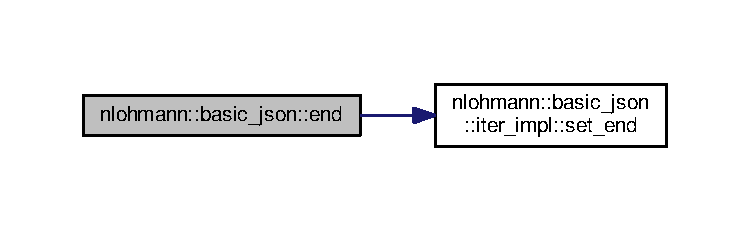
\includegraphics[width=350pt]{classnlohmann_1_1basic__json_a13e032a02a7fd8a93fdddc2fcbc4763c_cgraph}
\end{center}
\end{figure}
\mbox{\Hypertarget{classnlohmann_1_1basic__json_a1c15707055088cd5436ae91db72cbe67}\label{classnlohmann_1_1basic__json_a1c15707055088cd5436ae91db72cbe67}} 
\index{nlohmann\+::basic\+\_\+json@{nlohmann\+::basic\+\_\+json}!end@{end}}
\index{end@{end}!nlohmann\+::basic\+\_\+json@{nlohmann\+::basic\+\_\+json}}
\subsubsection{\texorpdfstring{end()}{end()}\hspace{0.1cm}{\footnotesize\ttfamily [2/2]}}
{\footnotesize\ttfamily template$<$template$<$ typename U, typename V, typename... Args $>$ class Object\+Type = std\+::map, template$<$ typename U, typename... Args $>$ class Array\+Type = std\+::vector, class String\+Type  = std\+::string, class Boolean\+Type  = bool, class Number\+Integer\+Type  = std\+::int64\+\_\+t, class Number\+Unsigned\+Type  = std\+::uint64\+\_\+t, class Number\+Float\+Type  = double, template$<$ typename U $>$ class Allocator\+Type = std\+::allocator, template$<$ typename T, typename S\+F\+I\+N\+A\+E=void $>$ class J\+S\+O\+N\+Serializer = adl\+\_\+serializer$>$ \\
\hyperlink{classnlohmann_1_1basic__json_a41a70cf9993951836d129bb1c2b3126a}{const\+\_\+iterator} \hyperlink{classnlohmann_1_1basic__json}{nlohmann\+::basic\+\_\+json}$<$ Object\+Type, Array\+Type, String\+Type, Boolean\+Type, Number\+Integer\+Type, Number\+Unsigned\+Type, Number\+Float\+Type, Allocator\+Type, J\+S\+O\+N\+Serializer $>$\+::end (\begin{DoxyParamCaption}{ }\end{DoxyParamCaption}) const\hspace{0.3cm}{\ttfamily [inline]}, {\ttfamily [noexcept]}}



returns a const iterator to one past the last element 

Returns a const iterator to one past the last element.

 \begin{DoxyReturn}{Returns}
const iterator one past the last element
\end{DoxyReturn}
Constant.

This function helps {\ttfamily \hyperlink{classnlohmann_1_1basic__json}{basic\+\_\+json}} satisfying the \href{http://en.cppreference.com/w/cpp/concept/Container}{\tt Container} requirements\+:
\begin{DoxyItemize}
\item The complexity is constant.
\item Has the semantics of {\ttfamily const\+\_\+cast$<$const \hyperlink{classnlohmann_1_1basic__json}{basic\+\_\+json}\&$>$($\ast$this).\hyperlink{classnlohmann_1_1basic__json_a13e032a02a7fd8a93fdddc2fcbc4763c}{end()}}.
\end{DoxyItemize}

\{The following code shows an example for {\ttfamily \hyperlink{classnlohmann_1_1basic__json_a8dba7b7d2f38e6b0c614030aa43983f6}{cend()}}.,cend\}

\begin{DoxySeeAlso}{See also}
\hyperlink{classnlohmann_1_1basic__json_a13e032a02a7fd8a93fdddc2fcbc4763c}{end()} -- returns an \hyperlink{classnlohmann_1_1basic__json_a099316232c76c034030a38faa6e34dca}{iterator} to the \hyperlink{classnlohmann_1_1basic__json_a13e032a02a7fd8a93fdddc2fcbc4763c}{end} 

\hyperlink{classnlohmann_1_1basic__json_a0ff28dac23f2bdecee9564d07f51dcdc}{begin()} -- returns an \hyperlink{classnlohmann_1_1basic__json_a099316232c76c034030a38faa6e34dca}{iterator} to the beginning 

\hyperlink{classnlohmann_1_1basic__json_ad865d6c291b237ae508d5cb2146b5877}{cbegin()} -- returns a const \hyperlink{classnlohmann_1_1basic__json_a099316232c76c034030a38faa6e34dca}{iterator} to the beginning
\end{DoxySeeAlso}
\begin{DoxySince}{Since}
version 1.\+0.\+0 
\end{DoxySince}
\mbox{\Hypertarget{classnlohmann_1_1basic__json_a068a16e76be178e83da6a192916923ed}\label{classnlohmann_1_1basic__json_a068a16e76be178e83da6a192916923ed}} 
\index{nlohmann\+::basic\+\_\+json@{nlohmann\+::basic\+\_\+json}!erase@{erase}}
\index{erase@{erase}!nlohmann\+::basic\+\_\+json@{nlohmann\+::basic\+\_\+json}}
\subsubsection{\texorpdfstring{erase()}{erase()}\hspace{0.1cm}{\footnotesize\ttfamily [1/4]}}
{\footnotesize\ttfamily template$<$template$<$ typename U, typename V, typename... Args $>$ class Object\+Type = std\+::map, template$<$ typename U, typename... Args $>$ class Array\+Type = std\+::vector, class String\+Type  = std\+::string, class Boolean\+Type  = bool, class Number\+Integer\+Type  = std\+::int64\+\_\+t, class Number\+Unsigned\+Type  = std\+::uint64\+\_\+t, class Number\+Float\+Type  = double, template$<$ typename U $>$ class Allocator\+Type = std\+::allocator, template$<$ typename T, typename S\+F\+I\+N\+A\+E=void $>$ class J\+S\+O\+N\+Serializer = adl\+\_\+serializer$>$ \\
template$<$class Iterator\+Type , typename std\+::enable\+\_\+if$<$ std\+::is\+\_\+same$<$ Iterator\+Type, typename basic\+\_\+json\+\_\+t\+::iterator $>$\+::value or std\+::is\+\_\+same$<$ Iterator\+Type, typename basic\+\_\+json\+\_\+t\+::const\+\_\+iterator $>$\+::value, int $>$\+::type  = 0$>$ \\
Iterator\+Type \hyperlink{classnlohmann_1_1basic__json}{nlohmann\+::basic\+\_\+json}$<$ Object\+Type, Array\+Type, String\+Type, Boolean\+Type, Number\+Integer\+Type, Number\+Unsigned\+Type, Number\+Float\+Type, Allocator\+Type, J\+S\+O\+N\+Serializer $>$\+::erase (\begin{DoxyParamCaption}\item[{Iterator\+Type}]{pos }\end{DoxyParamCaption})\hspace{0.3cm}{\ttfamily [inline]}}



remove element given an iterator 

Removes the element specified by iterator {\itshape pos}. The iterator {\itshape pos} must be valid and dereferenceable. Thus the {\ttfamily \hyperlink{classnlohmann_1_1basic__json_a13e032a02a7fd8a93fdddc2fcbc4763c}{end()}} iterator (which is valid, but is not dereferenceable) cannot be used as a value for {\itshape pos}.

If called on a primitive type other than {\ttfamily null}, the resulting J\+S\+ON value will be {\ttfamily null}.


\begin{DoxyParams}[1]{Parameters}
\mbox{\tt in}  & {\em pos} & iterator to the element to remove \\
\hline
\end{DoxyParams}
\begin{DoxyReturn}{Returns}
Iterator following the last removed element. If the iterator {\itshape pos} refers to the last element, the {\ttfamily \hyperlink{classnlohmann_1_1basic__json_a13e032a02a7fd8a93fdddc2fcbc4763c}{end()}} iterator is returned.
\end{DoxyReturn}

\begin{DoxyTemplParams}{Template Parameters}
{\em Iterator\+Type} & an \hyperlink{classnlohmann_1_1basic__json_a099316232c76c034030a38faa6e34dca}{iterator} or \hyperlink{classnlohmann_1_1basic__json_a41a70cf9993951836d129bb1c2b3126a}{const\+\_\+iterator}\\
\hline
\end{DoxyTemplParams}
\begin{DoxyPostcond}{Postcondition}
Invalidates iterators and references at or after the point of the erase, including the {\ttfamily \hyperlink{classnlohmann_1_1basic__json_a13e032a02a7fd8a93fdddc2fcbc4763c}{end()}} iterator.
\end{DoxyPostcond}

\begin{DoxyExceptions}{Exceptions}
{\em std\+::domain\+\_\+error} & if called on a {\ttfamily null} value; example\+: {\ttfamily \char`\"{}cannot
use erase() with null\char`\"{}} \\
\hline
{\em std\+::domain\+\_\+error} & if called on an iterator which does not belong to the current J\+S\+ON value; example\+: {\ttfamily \char`\"{}iterator does not fit current value\char`\"{}} \\
\hline
{\em std\+::out\+\_\+of\+\_\+range} & if called on a primitive type with invalid iterator (i.\+e., any iterator which is not {\ttfamily \hyperlink{classnlohmann_1_1basic__json_a0ff28dac23f2bdecee9564d07f51dcdc}{begin()}}); example\+: {\ttfamily \char`\"{}iterator
out of range\char`\"{}}\\
\hline
\end{DoxyExceptions}
The complexity depends on the type\+:
\begin{DoxyItemize}
\item objects\+: amortized constant
\item arrays\+: linear in distance between {\itshape pos} and the end of the container
\item strings\+: linear in the length of the string
\item other types\+: constant
\end{DoxyItemize}

\{The example shows the result of {\ttfamily \hyperlink{classnlohmann_1_1basic__json_a068a16e76be178e83da6a192916923ed}{erase()}} for different J\+S\+ON types.,erase\+\_\+\+\_\+\+Iterator\+Type\}

\begin{DoxySeeAlso}{See also}
\hyperlink{classnlohmann_1_1basic__json_a4b3f7eb2d4625d95a51fbbdceb7c5f39}{erase(\+Iterator\+Type, Iterator\+Type)} -- removes the elements in the given range 

\hyperlink{classnlohmann_1_1basic__json_a2f8484d69c55d8f2a9697a7bec29362a}{erase(const typename object\+\_\+t\+::key\+\_\+type\&)} -- removes the element from an \hyperlink{classnlohmann_1_1basic__json_a9f42ee7d10eee2d5a73fd94ca7f767ca}{object} \hyperlink{classnlohmann_1_1basic__json_a73ae333487310e3302135189ce8ff5d8}{at} the given key 

\hyperlink{classnlohmann_1_1basic__json_a88cbcefe9a3f4d294bed0653550a5cb9}{erase(const size\+\_\+type)} -- removes the element from an \hyperlink{classnlohmann_1_1basic__json_a4a4ec75e4d2845d9bcf7a9e5458e4949}{array} \hyperlink{classnlohmann_1_1basic__json_a73ae333487310e3302135189ce8ff5d8}{at} the given index
\end{DoxySeeAlso}
\begin{DoxySince}{Since}
version 1.\+0.\+0 
\end{DoxySince}
\mbox{\Hypertarget{classnlohmann_1_1basic__json_a4b3f7eb2d4625d95a51fbbdceb7c5f39}\label{classnlohmann_1_1basic__json_a4b3f7eb2d4625d95a51fbbdceb7c5f39}} 
\index{nlohmann\+::basic\+\_\+json@{nlohmann\+::basic\+\_\+json}!erase@{erase}}
\index{erase@{erase}!nlohmann\+::basic\+\_\+json@{nlohmann\+::basic\+\_\+json}}
\subsubsection{\texorpdfstring{erase()}{erase()}\hspace{0.1cm}{\footnotesize\ttfamily [2/4]}}
{\footnotesize\ttfamily template$<$template$<$ typename U, typename V, typename... Args $>$ class Object\+Type = std\+::map, template$<$ typename U, typename... Args $>$ class Array\+Type = std\+::vector, class String\+Type  = std\+::string, class Boolean\+Type  = bool, class Number\+Integer\+Type  = std\+::int64\+\_\+t, class Number\+Unsigned\+Type  = std\+::uint64\+\_\+t, class Number\+Float\+Type  = double, template$<$ typename U $>$ class Allocator\+Type = std\+::allocator, template$<$ typename T, typename S\+F\+I\+N\+A\+E=void $>$ class J\+S\+O\+N\+Serializer = adl\+\_\+serializer$>$ \\
template$<$class Iterator\+Type , typename std\+::enable\+\_\+if$<$ std\+::is\+\_\+same$<$ Iterator\+Type, typename basic\+\_\+json\+\_\+t\+::iterator $>$\+::value or std\+::is\+\_\+same$<$ Iterator\+Type, typename basic\+\_\+json\+\_\+t\+::const\+\_\+iterator $>$\+::value, int $>$\+::type  = 0$>$ \\
Iterator\+Type \hyperlink{classnlohmann_1_1basic__json}{nlohmann\+::basic\+\_\+json}$<$ Object\+Type, Array\+Type, String\+Type, Boolean\+Type, Number\+Integer\+Type, Number\+Unsigned\+Type, Number\+Float\+Type, Allocator\+Type, J\+S\+O\+N\+Serializer $>$\+::erase (\begin{DoxyParamCaption}\item[{Iterator\+Type}]{first,  }\item[{Iterator\+Type}]{last }\end{DoxyParamCaption})\hspace{0.3cm}{\ttfamily [inline]}}



remove elements given an iterator range 

Removes the element specified by the range {\ttfamily \mbox{[}first; last)}. The iterator {\itshape first} does not need to be dereferenceable if {\ttfamily first == last}\+: erasing an empty range is a no-\/op.

If called on a primitive type other than {\ttfamily null}, the resulting J\+S\+ON value will be {\ttfamily null}.


\begin{DoxyParams}[1]{Parameters}
\mbox{\tt in}  & {\em first} & iterator to the beginning of the range to remove \\
\hline
\mbox{\tt in}  & {\em last} & iterator past the end of the range to remove \\
\hline
\end{DoxyParams}
\begin{DoxyReturn}{Returns}
Iterator following the last removed element. If the iterator {\itshape second} refers to the last element, the {\ttfamily \hyperlink{classnlohmann_1_1basic__json_a13e032a02a7fd8a93fdddc2fcbc4763c}{end()}} iterator is returned.
\end{DoxyReturn}

\begin{DoxyTemplParams}{Template Parameters}
{\em Iterator\+Type} & an \hyperlink{classnlohmann_1_1basic__json_a099316232c76c034030a38faa6e34dca}{iterator} or \hyperlink{classnlohmann_1_1basic__json_a41a70cf9993951836d129bb1c2b3126a}{const\+\_\+iterator}\\
\hline
\end{DoxyTemplParams}
\begin{DoxyPostcond}{Postcondition}
Invalidates iterators and references at or after the point of the erase, including the {\ttfamily \hyperlink{classnlohmann_1_1basic__json_a13e032a02a7fd8a93fdddc2fcbc4763c}{end()}} iterator.
\end{DoxyPostcond}

\begin{DoxyExceptions}{Exceptions}
{\em std\+::domain\+\_\+error} & if called on a {\ttfamily null} value; example\+: {\ttfamily \char`\"{}cannot
use erase() with null\char`\"{}} \\
\hline
{\em std\+::domain\+\_\+error} & if called on iterators which does not belong to the current J\+S\+ON value; example\+: {\ttfamily \char`\"{}iterators do not fit current value\char`\"{}} \\
\hline
{\em std\+::out\+\_\+of\+\_\+range} & if called on a primitive type with invalid iterators (i.\+e., if {\ttfamily first != \hyperlink{classnlohmann_1_1basic__json_a0ff28dac23f2bdecee9564d07f51dcdc}{begin()}} and {\ttfamily last != \hyperlink{classnlohmann_1_1basic__json_a13e032a02a7fd8a93fdddc2fcbc4763c}{end()}}); example\+: {\ttfamily \char`\"{}iterators out of range\char`\"{}}\\
\hline
\end{DoxyExceptions}
The complexity depends on the type\+:
\begin{DoxyItemize}
\item objects\+: {\ttfamily log(size()) + std\+::distance(first, last)}
\item arrays\+: linear in the distance between {\itshape first} and {\itshape last}, plus linear in the distance between {\itshape last} and end of the container
\item strings\+: linear in the length of the string
\item other types\+: constant
\end{DoxyItemize}

\{The example shows the result of {\ttfamily \hyperlink{classnlohmann_1_1basic__json_a068a16e76be178e83da6a192916923ed}{erase()}} for different J\+S\+ON types.,erase\+\_\+\+\_\+\+Iterator\+Type\+\_\+\+Iterator\+Type\}

\begin{DoxySeeAlso}{See also}
\hyperlink{classnlohmann_1_1basic__json_a068a16e76be178e83da6a192916923ed}{erase(\+Iterator\+Type)} -- removes the element \hyperlink{classnlohmann_1_1basic__json_a73ae333487310e3302135189ce8ff5d8}{at} a given position 

\hyperlink{classnlohmann_1_1basic__json_a2f8484d69c55d8f2a9697a7bec29362a}{erase(const typename object\+\_\+t\+::key\+\_\+type\&)} -- removes the element from an \hyperlink{classnlohmann_1_1basic__json_a9f42ee7d10eee2d5a73fd94ca7f767ca}{object} \hyperlink{classnlohmann_1_1basic__json_a73ae333487310e3302135189ce8ff5d8}{at} the given key 

\hyperlink{classnlohmann_1_1basic__json_a88cbcefe9a3f4d294bed0653550a5cb9}{erase(const size\+\_\+type)} -- removes the element from an \hyperlink{classnlohmann_1_1basic__json_a4a4ec75e4d2845d9bcf7a9e5458e4949}{array} \hyperlink{classnlohmann_1_1basic__json_a73ae333487310e3302135189ce8ff5d8}{at} the given index
\end{DoxySeeAlso}
\begin{DoxySince}{Since}
version 1.\+0.\+0 
\end{DoxySince}
\mbox{\Hypertarget{classnlohmann_1_1basic__json_a2f8484d69c55d8f2a9697a7bec29362a}\label{classnlohmann_1_1basic__json_a2f8484d69c55d8f2a9697a7bec29362a}} 
\index{nlohmann\+::basic\+\_\+json@{nlohmann\+::basic\+\_\+json}!erase@{erase}}
\index{erase@{erase}!nlohmann\+::basic\+\_\+json@{nlohmann\+::basic\+\_\+json}}
\subsubsection{\texorpdfstring{erase()}{erase()}\hspace{0.1cm}{\footnotesize\ttfamily [3/4]}}
{\footnotesize\ttfamily template$<$template$<$ typename U, typename V, typename... Args $>$ class Object\+Type = std\+::map, template$<$ typename U, typename... Args $>$ class Array\+Type = std\+::vector, class String\+Type  = std\+::string, class Boolean\+Type  = bool, class Number\+Integer\+Type  = std\+::int64\+\_\+t, class Number\+Unsigned\+Type  = std\+::uint64\+\_\+t, class Number\+Float\+Type  = double, template$<$ typename U $>$ class Allocator\+Type = std\+::allocator, template$<$ typename T, typename S\+F\+I\+N\+A\+E=void $>$ class J\+S\+O\+N\+Serializer = adl\+\_\+serializer$>$ \\
\hyperlink{classnlohmann_1_1basic__json_a39f2cd0b58106097e0e67bf185cc519b}{size\+\_\+type} \hyperlink{classnlohmann_1_1basic__json}{nlohmann\+::basic\+\_\+json}$<$ Object\+Type, Array\+Type, String\+Type, Boolean\+Type, Number\+Integer\+Type, Number\+Unsigned\+Type, Number\+Float\+Type, Allocator\+Type, J\+S\+O\+N\+Serializer $>$\+::erase (\begin{DoxyParamCaption}\item[{const typename object\+\_\+t\+::key\+\_\+type \&}]{key }\end{DoxyParamCaption})\hspace{0.3cm}{\ttfamily [inline]}}



remove element from a J\+S\+ON object given a key 

Removes elements from a J\+S\+ON object with the key value {\itshape key}.


\begin{DoxyParams}[1]{Parameters}
\mbox{\tt in}  & {\em key} & value of the elements to remove\\
\hline
\end{DoxyParams}
\begin{DoxyReturn}{Returns}
Number of elements removed. If {\itshape Object\+Type} is the default {\ttfamily std\+::map} type, the return value will always be {\ttfamily 0} ({\itshape key} was not found) or {\ttfamily 1} ({\itshape key} was found).
\end{DoxyReturn}
\begin{DoxyPostcond}{Postcondition}
References and iterators to the erased elements are invalidated. Other references and iterators are not affected.
\end{DoxyPostcond}

\begin{DoxyExceptions}{Exceptions}
{\em std\+::domain\+\_\+error} & when called on a type other than J\+S\+ON object; example\+: {\ttfamily \char`\"{}cannot use erase() with null\char`\"{}}\\
\hline
\end{DoxyExceptions}
{\ttfamily log(size()) + count(key)}

\{The example shows the effect of {\ttfamily \hyperlink{classnlohmann_1_1basic__json_a068a16e76be178e83da6a192916923ed}{erase()}}.,erase\+\_\+\+\_\+key\+\_\+type\}

\begin{DoxySeeAlso}{See also}
\hyperlink{classnlohmann_1_1basic__json_a068a16e76be178e83da6a192916923ed}{erase(\+Iterator\+Type)} -- removes the element \hyperlink{classnlohmann_1_1basic__json_a73ae333487310e3302135189ce8ff5d8}{at} a given position 

\hyperlink{classnlohmann_1_1basic__json_a4b3f7eb2d4625d95a51fbbdceb7c5f39}{erase(\+Iterator\+Type, Iterator\+Type)} -- removes the elements in the given range 

\hyperlink{classnlohmann_1_1basic__json_a88cbcefe9a3f4d294bed0653550a5cb9}{erase(const size\+\_\+type)} -- removes the element from an \hyperlink{classnlohmann_1_1basic__json_a4a4ec75e4d2845d9bcf7a9e5458e4949}{array} \hyperlink{classnlohmann_1_1basic__json_a73ae333487310e3302135189ce8ff5d8}{at} the given index
\end{DoxySeeAlso}
\begin{DoxySince}{Since}
version 1.\+0.\+0 
\end{DoxySince}
\mbox{\Hypertarget{classnlohmann_1_1basic__json_a88cbcefe9a3f4d294bed0653550a5cb9}\label{classnlohmann_1_1basic__json_a88cbcefe9a3f4d294bed0653550a5cb9}} 
\index{nlohmann\+::basic\+\_\+json@{nlohmann\+::basic\+\_\+json}!erase@{erase}}
\index{erase@{erase}!nlohmann\+::basic\+\_\+json@{nlohmann\+::basic\+\_\+json}}
\subsubsection{\texorpdfstring{erase()}{erase()}\hspace{0.1cm}{\footnotesize\ttfamily [4/4]}}
{\footnotesize\ttfamily template$<$template$<$ typename U, typename V, typename... Args $>$ class Object\+Type = std\+::map, template$<$ typename U, typename... Args $>$ class Array\+Type = std\+::vector, class String\+Type  = std\+::string, class Boolean\+Type  = bool, class Number\+Integer\+Type  = std\+::int64\+\_\+t, class Number\+Unsigned\+Type  = std\+::uint64\+\_\+t, class Number\+Float\+Type  = double, template$<$ typename U $>$ class Allocator\+Type = std\+::allocator, template$<$ typename T, typename S\+F\+I\+N\+A\+E=void $>$ class J\+S\+O\+N\+Serializer = adl\+\_\+serializer$>$ \\
void \hyperlink{classnlohmann_1_1basic__json}{nlohmann\+::basic\+\_\+json}$<$ Object\+Type, Array\+Type, String\+Type, Boolean\+Type, Number\+Integer\+Type, Number\+Unsigned\+Type, Number\+Float\+Type, Allocator\+Type, J\+S\+O\+N\+Serializer $>$\+::erase (\begin{DoxyParamCaption}\item[{const \hyperlink{classnlohmann_1_1basic__json_a39f2cd0b58106097e0e67bf185cc519b}{size\+\_\+type}}]{idx }\end{DoxyParamCaption})\hspace{0.3cm}{\ttfamily [inline]}}



remove element from a J\+S\+ON array given an index 

Removes element from a J\+S\+ON array at the index {\itshape idx}.


\begin{DoxyParams}[1]{Parameters}
\mbox{\tt in}  & {\em idx} & index of the element to remove\\
\hline
\end{DoxyParams}

\begin{DoxyExceptions}{Exceptions}
{\em std\+::domain\+\_\+error} & when called on a type other than J\+S\+ON array; example\+: {\ttfamily \char`\"{}cannot use erase() with null\char`\"{}} \\
\hline
{\em std\+::out\+\_\+of\+\_\+range} & when {\ttfamily idx $>$= \hyperlink{classnlohmann_1_1basic__json_a25e27ad0c6d53c01871c5485e1f75b96}{size()}}; example\+: {\ttfamily \char`\"{}array index 17
is out of range\char`\"{}}\\
\hline
\end{DoxyExceptions}
Linear in distance between {\itshape idx} and the end of the container.

\{The example shows the effect of {\ttfamily \hyperlink{classnlohmann_1_1basic__json_a068a16e76be178e83da6a192916923ed}{erase()}}.,erase\+\_\+\+\_\+size\+\_\+type\}

\begin{DoxySeeAlso}{See also}
\hyperlink{classnlohmann_1_1basic__json_a068a16e76be178e83da6a192916923ed}{erase(\+Iterator\+Type)} -- removes the element \hyperlink{classnlohmann_1_1basic__json_a73ae333487310e3302135189ce8ff5d8}{at} a given position 

\hyperlink{classnlohmann_1_1basic__json_a4b3f7eb2d4625d95a51fbbdceb7c5f39}{erase(\+Iterator\+Type, Iterator\+Type)} -- removes the elements in the given range 

\hyperlink{classnlohmann_1_1basic__json_a2f8484d69c55d8f2a9697a7bec29362a}{erase(const typename object\+\_\+t\+::key\+\_\+type\&)} -- removes the element from an \hyperlink{classnlohmann_1_1basic__json_a9f42ee7d10eee2d5a73fd94ca7f767ca}{object} \hyperlink{classnlohmann_1_1basic__json_a73ae333487310e3302135189ce8ff5d8}{at} the given key
\end{DoxySeeAlso}
\begin{DoxySince}{Since}
version 1.\+0.\+0 
\end{DoxySince}
\mbox{\Hypertarget{classnlohmann_1_1basic__json_af6e1e06b6c274734ccb7de1ef770a915}\label{classnlohmann_1_1basic__json_af6e1e06b6c274734ccb7de1ef770a915}} 
\index{nlohmann\+::basic\+\_\+json@{nlohmann\+::basic\+\_\+json}!escape\+\_\+string@{escape\+\_\+string}}
\index{escape\+\_\+string@{escape\+\_\+string}!nlohmann\+::basic\+\_\+json@{nlohmann\+::basic\+\_\+json}}
\subsubsection{\texorpdfstring{escape\+\_\+string()}{escape\_string()}}
{\footnotesize\ttfamily template$<$template$<$ typename U, typename V, typename... Args $>$ class Object\+Type = std\+::map, template$<$ typename U, typename... Args $>$ class Array\+Type = std\+::vector, class String\+Type  = std\+::string, class Boolean\+Type  = bool, class Number\+Integer\+Type  = std\+::int64\+\_\+t, class Number\+Unsigned\+Type  = std\+::uint64\+\_\+t, class Number\+Float\+Type  = double, template$<$ typename U $>$ class Allocator\+Type = std\+::allocator, template$<$ typename T, typename S\+F\+I\+N\+A\+E=void $>$ class J\+S\+O\+N\+Serializer = adl\+\_\+serializer$>$ \\
static \hyperlink{classnlohmann_1_1basic__json_a61f8566a1a85a424c7266fb531dca005}{string\+\_\+t} \hyperlink{classnlohmann_1_1basic__json}{nlohmann\+::basic\+\_\+json}$<$ Object\+Type, Array\+Type, String\+Type, Boolean\+Type, Number\+Integer\+Type, Number\+Unsigned\+Type, Number\+Float\+Type, Allocator\+Type, J\+S\+O\+N\+Serializer $>$\+::escape\+\_\+string (\begin{DoxyParamCaption}\item[{const \hyperlink{classnlohmann_1_1basic__json_a61f8566a1a85a424c7266fb531dca005}{string\+\_\+t} \&}]{s }\end{DoxyParamCaption})\hspace{0.3cm}{\ttfamily [inline]}, {\ttfamily [static]}, {\ttfamily [private]}}



escape a string 

Escape a string by replacing certain special characters by a sequence of an escape character (backslash) and another character and other control characters by a sequence of \char`\"{}\textbackslash{}u\char`\"{} followed by a four-\/digit hex representation.


\begin{DoxyParams}[1]{Parameters}
\mbox{\tt in}  & {\em s} & the string to escape \\
\hline
\end{DoxyParams}
\begin{DoxyReturn}{Returns}
the escaped string
\end{DoxyReturn}
Linear in the length of string {\itshape s}. \mbox{\Hypertarget{classnlohmann_1_1basic__json_ab47d5e44bf890f791a597b1f55afb38e}\label{classnlohmann_1_1basic__json_ab47d5e44bf890f791a597b1f55afb38e}} 
\index{nlohmann\+::basic\+\_\+json@{nlohmann\+::basic\+\_\+json}!extra\+\_\+space@{extra\+\_\+space}}
\index{extra\+\_\+space@{extra\+\_\+space}!nlohmann\+::basic\+\_\+json@{nlohmann\+::basic\+\_\+json}}
\subsubsection{\texorpdfstring{extra\+\_\+space()}{extra\_space()}}
{\footnotesize\ttfamily template$<$template$<$ typename U, typename V, typename... Args $>$ class Object\+Type = std\+::map, template$<$ typename U, typename... Args $>$ class Array\+Type = std\+::vector, class String\+Type  = std\+::string, class Boolean\+Type  = bool, class Number\+Integer\+Type  = std\+::int64\+\_\+t, class Number\+Unsigned\+Type  = std\+::uint64\+\_\+t, class Number\+Float\+Type  = double, template$<$ typename U $>$ class Allocator\+Type = std\+::allocator, template$<$ typename T, typename S\+F\+I\+N\+A\+E=void $>$ class J\+S\+O\+N\+Serializer = adl\+\_\+serializer$>$ \\
static std\+::size\+\_\+t \hyperlink{classnlohmann_1_1basic__json}{nlohmann\+::basic\+\_\+json}$<$ Object\+Type, Array\+Type, String\+Type, Boolean\+Type, Number\+Integer\+Type, Number\+Unsigned\+Type, Number\+Float\+Type, Allocator\+Type, J\+S\+O\+N\+Serializer $>$\+::extra\+\_\+space (\begin{DoxyParamCaption}\item[{const \hyperlink{classnlohmann_1_1basic__json_a61f8566a1a85a424c7266fb531dca005}{string\+\_\+t} \&}]{s }\end{DoxyParamCaption})\hspace{0.3cm}{\ttfamily [inline]}, {\ttfamily [static]}, {\ttfamily [private]}, {\ttfamily [noexcept]}}



calculates the extra space to escape a J\+S\+ON string 


\begin{DoxyParams}[1]{Parameters}
\mbox{\tt in}  & {\em s} & the string to escape \\
\hline
\end{DoxyParams}
\begin{DoxyReturn}{Returns}
the number of characters required to escape string {\itshape s} 
\end{DoxyReturn}
Linear in the length of string {\itshape s}. \mbox{\Hypertarget{classnlohmann_1_1basic__json_aeed33787bd362c7ead59a4ba945392db}\label{classnlohmann_1_1basic__json_aeed33787bd362c7ead59a4ba945392db}} 
\index{nlohmann\+::basic\+\_\+json@{nlohmann\+::basic\+\_\+json}!find@{find}}
\index{find@{find}!nlohmann\+::basic\+\_\+json@{nlohmann\+::basic\+\_\+json}}
\subsubsection{\texorpdfstring{find()}{find()}\hspace{0.1cm}{\footnotesize\ttfamily [1/2]}}
{\footnotesize\ttfamily template$<$template$<$ typename U, typename V, typename... Args $>$ class Object\+Type = std\+::map, template$<$ typename U, typename... Args $>$ class Array\+Type = std\+::vector, class String\+Type  = std\+::string, class Boolean\+Type  = bool, class Number\+Integer\+Type  = std\+::int64\+\_\+t, class Number\+Unsigned\+Type  = std\+::uint64\+\_\+t, class Number\+Float\+Type  = double, template$<$ typename U $>$ class Allocator\+Type = std\+::allocator, template$<$ typename T, typename S\+F\+I\+N\+A\+E=void $>$ class J\+S\+O\+N\+Serializer = adl\+\_\+serializer$>$ \\
\hyperlink{classnlohmann_1_1basic__json_a099316232c76c034030a38faa6e34dca}{iterator} \hyperlink{classnlohmann_1_1basic__json}{nlohmann\+::basic\+\_\+json}$<$ Object\+Type, Array\+Type, String\+Type, Boolean\+Type, Number\+Integer\+Type, Number\+Unsigned\+Type, Number\+Float\+Type, Allocator\+Type, J\+S\+O\+N\+Serializer $>$\+::find (\begin{DoxyParamCaption}\item[{typename object\+\_\+t\+::key\+\_\+type}]{key }\end{DoxyParamCaption})\hspace{0.3cm}{\ttfamily [inline]}}



find an element in a J\+S\+ON object 

Finds an element in a J\+S\+ON object with key equivalent to {\itshape key}. If the element is not found or the J\+S\+ON value is not an object, \hyperlink{classnlohmann_1_1basic__json_a13e032a02a7fd8a93fdddc2fcbc4763c}{end()} is returned.

\begin{DoxyNote}{Note}
This method always returns \hyperlink{classnlohmann_1_1basic__json_a13e032a02a7fd8a93fdddc2fcbc4763c}{end()} when executed on a J\+S\+ON type that is not an object.
\end{DoxyNote}

\begin{DoxyParams}[1]{Parameters}
\mbox{\tt in}  & {\em key} & key value of the element to search for\\
\hline
\end{DoxyParams}
\begin{DoxyReturn}{Returns}
Iterator to an element with key equivalent to {\itshape key}. If no such element is found or the J\+S\+ON value is not an object, past-\/the-\/end (see \hyperlink{classnlohmann_1_1basic__json_a13e032a02a7fd8a93fdddc2fcbc4763c}{end()}) iterator is returned.
\end{DoxyReturn}
Logarithmic in the size of the J\+S\+ON object.

\{The example shows how {\ttfamily \hyperlink{classnlohmann_1_1basic__json_aeed33787bd362c7ead59a4ba945392db}{find()}} is used.,find\+\_\+\+\_\+key\+\_\+type\}

\begin{DoxySince}{Since}
version 1.\+0.\+0 
\end{DoxySince}
\mbox{\Hypertarget{classnlohmann_1_1basic__json_a6d2f26a0a84787a43c989c88e2b7023b}\label{classnlohmann_1_1basic__json_a6d2f26a0a84787a43c989c88e2b7023b}} 
\index{nlohmann\+::basic\+\_\+json@{nlohmann\+::basic\+\_\+json}!find@{find}}
\index{find@{find}!nlohmann\+::basic\+\_\+json@{nlohmann\+::basic\+\_\+json}}
\subsubsection{\texorpdfstring{find()}{find()}\hspace{0.1cm}{\footnotesize\ttfamily [2/2]}}
{\footnotesize\ttfamily template$<$template$<$ typename U, typename V, typename... Args $>$ class Object\+Type = std\+::map, template$<$ typename U, typename... Args $>$ class Array\+Type = std\+::vector, class String\+Type  = std\+::string, class Boolean\+Type  = bool, class Number\+Integer\+Type  = std\+::int64\+\_\+t, class Number\+Unsigned\+Type  = std\+::uint64\+\_\+t, class Number\+Float\+Type  = double, template$<$ typename U $>$ class Allocator\+Type = std\+::allocator, template$<$ typename T, typename S\+F\+I\+N\+A\+E=void $>$ class J\+S\+O\+N\+Serializer = adl\+\_\+serializer$>$ \\
\hyperlink{classnlohmann_1_1basic__json_a41a70cf9993951836d129bb1c2b3126a}{const\+\_\+iterator} \hyperlink{classnlohmann_1_1basic__json}{nlohmann\+::basic\+\_\+json}$<$ Object\+Type, Array\+Type, String\+Type, Boolean\+Type, Number\+Integer\+Type, Number\+Unsigned\+Type, Number\+Float\+Type, Allocator\+Type, J\+S\+O\+N\+Serializer $>$\+::find (\begin{DoxyParamCaption}\item[{typename object\+\_\+t\+::key\+\_\+type}]{key }\end{DoxyParamCaption}) const\hspace{0.3cm}{\ttfamily [inline]}}



find an element in a J\+S\+ON object 

find an element in a J\+S\+ON object Finds an element in a J\+S\+ON object with key equivalent to {\itshape key}. If the element is not found or the J\+S\+ON value is not an object, \hyperlink{classnlohmann_1_1basic__json_a13e032a02a7fd8a93fdddc2fcbc4763c}{end()} is returned.

\begin{DoxyNote}{Note}
This method always returns \hyperlink{classnlohmann_1_1basic__json_a13e032a02a7fd8a93fdddc2fcbc4763c}{end()} when executed on a J\+S\+ON type that is not an object.
\end{DoxyNote}

\begin{DoxyParams}[1]{Parameters}
\mbox{\tt in}  & {\em key} & key value of the element to search for\\
\hline
\end{DoxyParams}
\begin{DoxyReturn}{Returns}
Iterator to an element with key equivalent to {\itshape key}. If no such element is found or the J\+S\+ON value is not an object, past-\/the-\/end (see \hyperlink{classnlohmann_1_1basic__json_a13e032a02a7fd8a93fdddc2fcbc4763c}{end()}) iterator is returned.
\end{DoxyReturn}
Logarithmic in the size of the J\+S\+ON object.

\{The example shows how {\ttfamily \hyperlink{classnlohmann_1_1basic__json_aeed33787bd362c7ead59a4ba945392db}{find()}} is used.,find\+\_\+\+\_\+key\+\_\+type\}

\begin{DoxySince}{Since}
version 1.\+0.\+0 
\end{DoxySince}
\mbox{\Hypertarget{classnlohmann_1_1basic__json_ab838f000d76662917ffd6ec529569e03}\label{classnlohmann_1_1basic__json_ab838f000d76662917ffd6ec529569e03}} 
\index{nlohmann\+::basic\+\_\+json@{nlohmann\+::basic\+\_\+json}!flatten@{flatten}}
\index{flatten@{flatten}!nlohmann\+::basic\+\_\+json@{nlohmann\+::basic\+\_\+json}}
\subsubsection{\texorpdfstring{flatten()}{flatten()}}
{\footnotesize\ttfamily template$<$template$<$ typename U, typename V, typename... Args $>$ class Object\+Type = std\+::map, template$<$ typename U, typename... Args $>$ class Array\+Type = std\+::vector, class String\+Type  = std\+::string, class Boolean\+Type  = bool, class Number\+Integer\+Type  = std\+::int64\+\_\+t, class Number\+Unsigned\+Type  = std\+::uint64\+\_\+t, class Number\+Float\+Type  = double, template$<$ typename U $>$ class Allocator\+Type = std\+::allocator, template$<$ typename T, typename S\+F\+I\+N\+A\+E=void $>$ class J\+S\+O\+N\+Serializer = adl\+\_\+serializer$>$ \\
\hyperlink{classnlohmann_1_1basic__json}{basic\+\_\+json} \hyperlink{classnlohmann_1_1basic__json}{nlohmann\+::basic\+\_\+json}$<$ Object\+Type, Array\+Type, String\+Type, Boolean\+Type, Number\+Integer\+Type, Number\+Unsigned\+Type, Number\+Float\+Type, Allocator\+Type, J\+S\+O\+N\+Serializer $>$\+::flatten (\begin{DoxyParamCaption}{ }\end{DoxyParamCaption}) const\hspace{0.3cm}{\ttfamily [inline]}}



return flattened J\+S\+ON value 

The function creates a J\+S\+ON object whose keys are J\+S\+ON pointers (see \href{https://tools.ietf.org/html/rfc6901}{\tt R\+FC 6901}) and whose values are all primitive. The original J\+S\+ON value can be restored using the \hyperlink{classnlohmann_1_1basic__json_a74fa3ab2003f2f6f2b69deaafed9126d}{unflatten()} function.

\begin{DoxyReturn}{Returns}
an object that maps J\+S\+ON pointers to primitive values
\end{DoxyReturn}
\begin{DoxyNote}{Note}
Empty objects and arrays are flattened to {\ttfamily null} and will not be reconstructed correctly by the \hyperlink{classnlohmann_1_1basic__json_a74fa3ab2003f2f6f2b69deaafed9126d}{unflatten()} function.
\end{DoxyNote}
Linear in the size the J\+S\+ON value.

\{The following code shows how a J\+S\+ON object is flattened to an object whose keys consist of J\+S\+ON pointers.,flatten\}

\begin{DoxySeeAlso}{See also}
\hyperlink{classnlohmann_1_1basic__json_a74fa3ab2003f2f6f2b69deaafed9126d}{unflatten()} for the reverse function
\end{DoxySeeAlso}
\begin{DoxySince}{Since}
version 2.\+0.\+0 
\end{DoxySince}
\mbox{\Hypertarget{classnlohmann_1_1basic__json_ab5e3e1758c1a52ffe89b1d379ef7fbe1}\label{classnlohmann_1_1basic__json_ab5e3e1758c1a52ffe89b1d379ef7fbe1}} 
\index{nlohmann\+::basic\+\_\+json@{nlohmann\+::basic\+\_\+json}!from\+\_\+cbor@{from\+\_\+cbor}}
\index{from\+\_\+cbor@{from\+\_\+cbor}!nlohmann\+::basic\+\_\+json@{nlohmann\+::basic\+\_\+json}}
\subsubsection{\texorpdfstring{from\+\_\+cbor()}{from\_cbor()}}
{\footnotesize\ttfamily template$<$template$<$ typename U, typename V, typename... Args $>$ class Object\+Type = std\+::map, template$<$ typename U, typename... Args $>$ class Array\+Type = std\+::vector, class String\+Type  = std\+::string, class Boolean\+Type  = bool, class Number\+Integer\+Type  = std\+::int64\+\_\+t, class Number\+Unsigned\+Type  = std\+::uint64\+\_\+t, class Number\+Float\+Type  = double, template$<$ typename U $>$ class Allocator\+Type = std\+::allocator, template$<$ typename T, typename S\+F\+I\+N\+A\+E=void $>$ class J\+S\+O\+N\+Serializer = adl\+\_\+serializer$>$ \\
static \hyperlink{classnlohmann_1_1basic__json}{basic\+\_\+json} \hyperlink{classnlohmann_1_1basic__json}{nlohmann\+::basic\+\_\+json}$<$ Object\+Type, Array\+Type, String\+Type, Boolean\+Type, Number\+Integer\+Type, Number\+Unsigned\+Type, Number\+Float\+Type, Allocator\+Type, J\+S\+O\+N\+Serializer $>$\+::from\+\_\+cbor (\begin{DoxyParamCaption}\item[{const std\+::vector$<$ uint8\+\_\+t $>$ \&}]{v,  }\item[{const size\+\_\+t}]{start\+\_\+index = {\ttfamily 0} }\end{DoxyParamCaption})\hspace{0.3cm}{\ttfamily [inline]}, {\ttfamily [static]}}



create a J\+S\+ON value from a byte vector in C\+B\+OR format 

Deserializes a given byte vector {\itshape v} to a J\+S\+ON value using the C\+B\+OR (Concise Binary Object Representation) serialization format.


\begin{DoxyParams}[1]{Parameters}
\mbox{\tt in}  & {\em v} & a byte vector in C\+B\+OR format \\
\hline
\mbox{\tt in}  & {\em start\+\_\+index} & the index to start reading from {\itshape v} (0 by default) \\
\hline
\end{DoxyParams}
\begin{DoxyReturn}{Returns}
deserialized J\+S\+ON value
\end{DoxyReturn}

\begin{DoxyExceptions}{Exceptions}
{\em std\+::invalid\+\_\+argument} & if unsupported features from C\+B\+OR were used in the given vector {\itshape v} or if the input is not valid Message\+Pack \\
\hline
{\em std\+::out\+\_\+of\+\_\+range} & if the given vector ends prematurely\\
\hline
\end{DoxyExceptions}
Linear in the size of the byte vector {\itshape v}.

\{The example shows the deserialization of a byte vector in C\+B\+OR format to a J\+S\+ON value.,from\+\_\+cbor\}

\begin{DoxySeeAlso}{See also}
\href{http://cbor.io}{\tt http\+://cbor.\+io} 

\hyperlink{classnlohmann_1_1basic__json_a2566783e190dec524bf3445b322873b8}{to\+\_\+cbor(const basic\+\_\+json\&)} for the analogous serialization 

\hyperlink{classnlohmann_1_1basic__json_a3eafe0b1fb2f2c443f1b3fea55c8a470}{from\+\_\+msgpack(const std\+::vector$<$uint8\+\_\+t$>$\&, const size\+\_\+t)} for the related Message\+Pack format
\end{DoxySeeAlso}
\begin{DoxySince}{Since}
version 2.\+0.\+9, parameter {\itshape start\+\_\+index} since 2.\+1.\+1 
\end{DoxySince}
\mbox{\Hypertarget{classnlohmann_1_1basic__json_a782368d422aa7bb3dca75361665bfcff}\label{classnlohmann_1_1basic__json_a782368d422aa7bb3dca75361665bfcff}} 
\index{nlohmann\+::basic\+\_\+json@{nlohmann\+::basic\+\_\+json}!from\+\_\+cbor\+\_\+internal@{from\+\_\+cbor\+\_\+internal}}
\index{from\+\_\+cbor\+\_\+internal@{from\+\_\+cbor\+\_\+internal}!nlohmann\+::basic\+\_\+json@{nlohmann\+::basic\+\_\+json}}
\subsubsection{\texorpdfstring{from\+\_\+cbor\+\_\+internal()}{from\_cbor\_internal()}}
{\footnotesize\ttfamily template$<$template$<$ typename U, typename V, typename... Args $>$ class Object\+Type = std\+::map, template$<$ typename U, typename... Args $>$ class Array\+Type = std\+::vector, class String\+Type  = std\+::string, class Boolean\+Type  = bool, class Number\+Integer\+Type  = std\+::int64\+\_\+t, class Number\+Unsigned\+Type  = std\+::uint64\+\_\+t, class Number\+Float\+Type  = double, template$<$ typename U $>$ class Allocator\+Type = std\+::allocator, template$<$ typename T, typename S\+F\+I\+N\+A\+E=void $>$ class J\+S\+O\+N\+Serializer = adl\+\_\+serializer$>$ \\
static \hyperlink{classnlohmann_1_1basic__json}{basic\+\_\+json} \hyperlink{classnlohmann_1_1basic__json}{nlohmann\+::basic\+\_\+json}$<$ Object\+Type, Array\+Type, String\+Type, Boolean\+Type, Number\+Integer\+Type, Number\+Unsigned\+Type, Number\+Float\+Type, Allocator\+Type, J\+S\+O\+N\+Serializer $>$\+::from\+\_\+cbor\+\_\+internal (\begin{DoxyParamCaption}\item[{const std\+::vector$<$ uint8\+\_\+t $>$ \&}]{v,  }\item[{size\+\_\+t \&}]{idx }\end{DoxyParamCaption})\hspace{0.3cm}{\ttfamily [inline]}, {\ttfamily [static]}, {\ttfamily [private]}}



create a J\+S\+ON value from a given C\+B\+OR vector 


\begin{DoxyParams}[1]{Parameters}
\mbox{\tt in}  & {\em v} & C\+B\+OR serialization \\
\hline
\mbox{\tt in}  & {\em idx} & byte index to start reading from {\itshape v} \\
\hline
\end{DoxyParams}
\begin{DoxyReturn}{Returns}
deserialized J\+S\+ON value
\end{DoxyReturn}

\begin{DoxyExceptions}{Exceptions}
{\em std\+::invalid\+\_\+argument} & if unsupported features from C\+B\+OR were used in the given vector {\itshape v} or if the input is not valid C\+B\+OR \\
\hline
{\em std\+::out\+\_\+of\+\_\+range} & if the given vector ends prematurely\\
\hline
\end{DoxyExceptions}
\begin{DoxySeeAlso}{See also}
\href{https://tools.ietf.org/html/rfc7049}{\tt https\+://tools.\+ietf.\+org/html/rfc7049} 
\end{DoxySeeAlso}
Here is the call graph for this function\+:\nopagebreak
\begin{figure}[H]
\begin{center}
\leavevmode
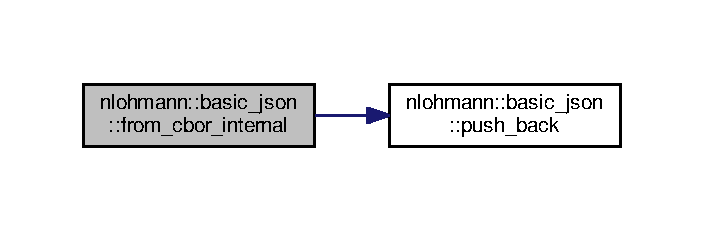
\includegraphics[width=338pt]{classnlohmann_1_1basic__json_a782368d422aa7bb3dca75361665bfcff_cgraph}
\end{center}
\end{figure}
\mbox{\Hypertarget{classnlohmann_1_1basic__json_a3eafe0b1fb2f2c443f1b3fea55c8a470}\label{classnlohmann_1_1basic__json_a3eafe0b1fb2f2c443f1b3fea55c8a470}} 
\index{nlohmann\+::basic\+\_\+json@{nlohmann\+::basic\+\_\+json}!from\+\_\+msgpack@{from\+\_\+msgpack}}
\index{from\+\_\+msgpack@{from\+\_\+msgpack}!nlohmann\+::basic\+\_\+json@{nlohmann\+::basic\+\_\+json}}
\subsubsection{\texorpdfstring{from\+\_\+msgpack()}{from\_msgpack()}}
{\footnotesize\ttfamily template$<$template$<$ typename U, typename V, typename... Args $>$ class Object\+Type = std\+::map, template$<$ typename U, typename... Args $>$ class Array\+Type = std\+::vector, class String\+Type  = std\+::string, class Boolean\+Type  = bool, class Number\+Integer\+Type  = std\+::int64\+\_\+t, class Number\+Unsigned\+Type  = std\+::uint64\+\_\+t, class Number\+Float\+Type  = double, template$<$ typename U $>$ class Allocator\+Type = std\+::allocator, template$<$ typename T, typename S\+F\+I\+N\+A\+E=void $>$ class J\+S\+O\+N\+Serializer = adl\+\_\+serializer$>$ \\
static \hyperlink{classnlohmann_1_1basic__json}{basic\+\_\+json} \hyperlink{classnlohmann_1_1basic__json}{nlohmann\+::basic\+\_\+json}$<$ Object\+Type, Array\+Type, String\+Type, Boolean\+Type, Number\+Integer\+Type, Number\+Unsigned\+Type, Number\+Float\+Type, Allocator\+Type, J\+S\+O\+N\+Serializer $>$\+::from\+\_\+msgpack (\begin{DoxyParamCaption}\item[{const std\+::vector$<$ uint8\+\_\+t $>$ \&}]{v,  }\item[{const size\+\_\+t}]{start\+\_\+index = {\ttfamily 0} }\end{DoxyParamCaption})\hspace{0.3cm}{\ttfamily [inline]}, {\ttfamily [static]}}



create a J\+S\+ON value from a byte vector in Message\+Pack format 

Deserializes a given byte vector {\itshape v} to a J\+S\+ON value using the Message\+Pack serialization format.


\begin{DoxyParams}[1]{Parameters}
\mbox{\tt in}  & {\em v} & a byte vector in Message\+Pack format \\
\hline
\mbox{\tt in}  & {\em start\+\_\+index} & the index to start reading from {\itshape v} (0 by default) \\
\hline
\end{DoxyParams}
\begin{DoxyReturn}{Returns}
deserialized J\+S\+ON value
\end{DoxyReturn}

\begin{DoxyExceptions}{Exceptions}
{\em std\+::invalid\+\_\+argument} & if unsupported features from Message\+Pack were used in the given vector {\itshape v} or if the input is not valid Message\+Pack \\
\hline
{\em std\+::out\+\_\+of\+\_\+range} & if the given vector ends prematurely\\
\hline
\end{DoxyExceptions}
Linear in the size of the byte vector {\itshape v}.

\{The example shows the deserialization of a byte vector in Message\+Pack format to a J\+S\+ON value.,from\+\_\+msgpack\}

\begin{DoxySeeAlso}{See also}
\href{http://msgpack.org}{\tt http\+://msgpack.\+org} 

\hyperlink{classnlohmann_1_1basic__json_a09ca1dc273d226afe0ca83a9d7438d9c}{to\+\_\+msgpack(const basic\+\_\+json\&)} for the analogous serialization 

\hyperlink{classnlohmann_1_1basic__json_ab5e3e1758c1a52ffe89b1d379ef7fbe1}{from\+\_\+cbor(const std\+::vector$<$uint8\+\_\+t$>$\&, const size\+\_\+t)} for the related C\+B\+OR format
\end{DoxySeeAlso}
\begin{DoxySince}{Since}
version 2.\+0.\+9, parameter {\itshape start\+\_\+index} since 2.\+1.\+1 
\end{DoxySince}
\mbox{\Hypertarget{classnlohmann_1_1basic__json_a2c758bc0a9b61177e4ec0d0c216bfe2b}\label{classnlohmann_1_1basic__json_a2c758bc0a9b61177e4ec0d0c216bfe2b}} 
\index{nlohmann\+::basic\+\_\+json@{nlohmann\+::basic\+\_\+json}!from\+\_\+msgpack\+\_\+internal@{from\+\_\+msgpack\+\_\+internal}}
\index{from\+\_\+msgpack\+\_\+internal@{from\+\_\+msgpack\+\_\+internal}!nlohmann\+::basic\+\_\+json@{nlohmann\+::basic\+\_\+json}}
\subsubsection{\texorpdfstring{from\+\_\+msgpack\+\_\+internal()}{from\_msgpack\_internal()}}
{\footnotesize\ttfamily template$<$template$<$ typename U, typename V, typename... Args $>$ class Object\+Type = std\+::map, template$<$ typename U, typename... Args $>$ class Array\+Type = std\+::vector, class String\+Type  = std\+::string, class Boolean\+Type  = bool, class Number\+Integer\+Type  = std\+::int64\+\_\+t, class Number\+Unsigned\+Type  = std\+::uint64\+\_\+t, class Number\+Float\+Type  = double, template$<$ typename U $>$ class Allocator\+Type = std\+::allocator, template$<$ typename T, typename S\+F\+I\+N\+A\+E=void $>$ class J\+S\+O\+N\+Serializer = adl\+\_\+serializer$>$ \\
static \hyperlink{classnlohmann_1_1basic__json}{basic\+\_\+json} \hyperlink{classnlohmann_1_1basic__json}{nlohmann\+::basic\+\_\+json}$<$ Object\+Type, Array\+Type, String\+Type, Boolean\+Type, Number\+Integer\+Type, Number\+Unsigned\+Type, Number\+Float\+Type, Allocator\+Type, J\+S\+O\+N\+Serializer $>$\+::from\+\_\+msgpack\+\_\+internal (\begin{DoxyParamCaption}\item[{const std\+::vector$<$ uint8\+\_\+t $>$ \&}]{v,  }\item[{size\+\_\+t \&}]{idx }\end{DoxyParamCaption})\hspace{0.3cm}{\ttfamily [inline]}, {\ttfamily [static]}, {\ttfamily [private]}}



create a J\+S\+ON value from a given Message\+Pack vector 


\begin{DoxyParams}[1]{Parameters}
\mbox{\tt in}  & {\em v} & Message\+Pack serialization \\
\hline
\mbox{\tt in}  & {\em idx} & byte index to start reading from {\itshape v} \\
\hline
\end{DoxyParams}
\begin{DoxyReturn}{Returns}
deserialized J\+S\+ON value
\end{DoxyReturn}

\begin{DoxyExceptions}{Exceptions}
{\em std\+::invalid\+\_\+argument} & if unsupported features from Message\+Pack were used in the given vector {\itshape v} or if the input is not valid Message\+Pack \\
\hline
{\em std\+::out\+\_\+of\+\_\+range} & if the given vector ends prematurely\\
\hline
\end{DoxyExceptions}
\begin{DoxySeeAlso}{See also}
\href{https://github.com/msgpack/msgpack/blob/master/spec.md}{\tt https\+://github.\+com/msgpack/msgpack/blob/master/spec.\+md} 
\end{DoxySeeAlso}
Here is the call graph for this function\+:\nopagebreak
\begin{figure}[H]
\begin{center}
\leavevmode
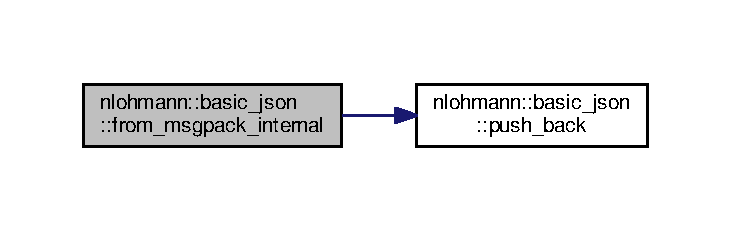
\includegraphics[width=350pt]{classnlohmann_1_1basic__json_a2c758bc0a9b61177e4ec0d0c216bfe2b_cgraph}
\end{center}
\end{figure}
\mbox{\Hypertarget{classnlohmann_1_1basic__json_a3acba9c6ceb7214e565fe08c3ba5b352}\label{classnlohmann_1_1basic__json_a3acba9c6ceb7214e565fe08c3ba5b352}} 
\index{nlohmann\+::basic\+\_\+json@{nlohmann\+::basic\+\_\+json}!front@{front}}
\index{front@{front}!nlohmann\+::basic\+\_\+json@{nlohmann\+::basic\+\_\+json}}
\subsubsection{\texorpdfstring{front()}{front()}\hspace{0.1cm}{\footnotesize\ttfamily [1/2]}}
{\footnotesize\ttfamily template$<$template$<$ typename U, typename V, typename... Args $>$ class Object\+Type = std\+::map, template$<$ typename U, typename... Args $>$ class Array\+Type = std\+::vector, class String\+Type  = std\+::string, class Boolean\+Type  = bool, class Number\+Integer\+Type  = std\+::int64\+\_\+t, class Number\+Unsigned\+Type  = std\+::uint64\+\_\+t, class Number\+Float\+Type  = double, template$<$ typename U $>$ class Allocator\+Type = std\+::allocator, template$<$ typename T, typename S\+F\+I\+N\+A\+E=void $>$ class J\+S\+O\+N\+Serializer = adl\+\_\+serializer$>$ \\
\hyperlink{classnlohmann_1_1basic__json_ac6a5eddd156c776ac75ff54cfe54a5bc}{reference} \hyperlink{classnlohmann_1_1basic__json}{nlohmann\+::basic\+\_\+json}$<$ Object\+Type, Array\+Type, String\+Type, Boolean\+Type, Number\+Integer\+Type, Number\+Unsigned\+Type, Number\+Float\+Type, Allocator\+Type, J\+S\+O\+N\+Serializer $>$\+::front (\begin{DoxyParamCaption}{ }\end{DoxyParamCaption})\hspace{0.3cm}{\ttfamily [inline]}}



access the first element 

Returns a reference to the first element in the container. For a J\+S\+ON container {\ttfamily c}, the expression {\ttfamily c.\+front()} is equivalent to {\ttfamily $\ast$c.\hyperlink{classnlohmann_1_1basic__json_a0ff28dac23f2bdecee9564d07f51dcdc}{begin()}}.

\begin{DoxyReturn}{Returns}
In case of a structured type (array or object), a reference to the first element is returned. In case of number, string, or boolean values, a reference to the value is returned.
\end{DoxyReturn}
Constant.

\begin{DoxyPrecond}{Precondition}
The J\+S\+ON value must not be {\ttfamily null} (would throw {\ttfamily std\+::out\+\_\+of\+\_\+range}) or an empty array or object (undefined behavior, {\bfseries guarded by assertions}). 
\end{DoxyPrecond}
\begin{DoxyPostcond}{Postcondition}
The J\+S\+ON value remains unchanged.
\end{DoxyPostcond}

\begin{DoxyExceptions}{Exceptions}
{\em std\+::out\+\_\+of\+\_\+range} & when called on {\ttfamily null} value\\
\hline
\end{DoxyExceptions}
\{The following code shows an example for {\ttfamily \hyperlink{classnlohmann_1_1basic__json_a3acba9c6ceb7214e565fe08c3ba5b352}{front()}}.,front\}

\begin{DoxySeeAlso}{See also}
\hyperlink{classnlohmann_1_1basic__json_a011397134847f36db0ed7d7a93753677}{back()} -- access the last element
\end{DoxySeeAlso}
\begin{DoxySince}{Since}
version 1.\+0.\+0 
\end{DoxySince}
\mbox{\Hypertarget{classnlohmann_1_1basic__json_a4b1fb3671ade9afc8d33b2c9510acbfc}\label{classnlohmann_1_1basic__json_a4b1fb3671ade9afc8d33b2c9510acbfc}} 
\index{nlohmann\+::basic\+\_\+json@{nlohmann\+::basic\+\_\+json}!front@{front}}
\index{front@{front}!nlohmann\+::basic\+\_\+json@{nlohmann\+::basic\+\_\+json}}
\subsubsection{\texorpdfstring{front()}{front()}\hspace{0.1cm}{\footnotesize\ttfamily [2/2]}}
{\footnotesize\ttfamily template$<$template$<$ typename U, typename V, typename... Args $>$ class Object\+Type = std\+::map, template$<$ typename U, typename... Args $>$ class Array\+Type = std\+::vector, class String\+Type  = std\+::string, class Boolean\+Type  = bool, class Number\+Integer\+Type  = std\+::int64\+\_\+t, class Number\+Unsigned\+Type  = std\+::uint64\+\_\+t, class Number\+Float\+Type  = double, template$<$ typename U $>$ class Allocator\+Type = std\+::allocator, template$<$ typename T, typename S\+F\+I\+N\+A\+E=void $>$ class J\+S\+O\+N\+Serializer = adl\+\_\+serializer$>$ \\
\hyperlink{classnlohmann_1_1basic__json_a4057c5425f4faacfe39a8046871786ca}{const\+\_\+reference} \hyperlink{classnlohmann_1_1basic__json}{nlohmann\+::basic\+\_\+json}$<$ Object\+Type, Array\+Type, String\+Type, Boolean\+Type, Number\+Integer\+Type, Number\+Unsigned\+Type, Number\+Float\+Type, Allocator\+Type, J\+S\+O\+N\+Serializer $>$\+::front (\begin{DoxyParamCaption}{ }\end{DoxyParamCaption}) const\hspace{0.3cm}{\ttfamily [inline]}}



access the first element 

Returns a reference to the first element in the container. For a J\+S\+ON container {\ttfamily c}, the expression {\ttfamily c.\+front()} is equivalent to {\ttfamily $\ast$c.\hyperlink{classnlohmann_1_1basic__json_a0ff28dac23f2bdecee9564d07f51dcdc}{begin()}}.

\begin{DoxyReturn}{Returns}
In case of a structured type (array or object), a reference to the first element is returned. In case of number, string, or boolean values, a reference to the value is returned.
\end{DoxyReturn}
Constant.

\begin{DoxyPrecond}{Precondition}
The J\+S\+ON value must not be {\ttfamily null} (would throw {\ttfamily std\+::out\+\_\+of\+\_\+range}) or an empty array or object (undefined behavior, {\bfseries guarded by assertions}). 
\end{DoxyPrecond}
\begin{DoxyPostcond}{Postcondition}
The J\+S\+ON value remains unchanged.
\end{DoxyPostcond}

\begin{DoxyExceptions}{Exceptions}
{\em std\+::out\+\_\+of\+\_\+range} & when called on {\ttfamily null} value\\
\hline
\end{DoxyExceptions}
\{The following code shows an example for {\ttfamily \hyperlink{classnlohmann_1_1basic__json_a3acba9c6ceb7214e565fe08c3ba5b352}{front()}}.,front\}

\begin{DoxySeeAlso}{See also}
\hyperlink{classnlohmann_1_1basic__json_a011397134847f36db0ed7d7a93753677}{back()} -- access the last element
\end{DoxySeeAlso}
\begin{DoxySince}{Since}
version 1.\+0.\+0 
\end{DoxySince}
\mbox{\Hypertarget{classnlohmann_1_1basic__json_a6b187a22994c12c8cae0dd5ee99dc85e}\label{classnlohmann_1_1basic__json_a6b187a22994c12c8cae0dd5ee99dc85e}} 
\index{nlohmann\+::basic\+\_\+json@{nlohmann\+::basic\+\_\+json}!get@{get}}
\index{get@{get}!nlohmann\+::basic\+\_\+json@{nlohmann\+::basic\+\_\+json}}
\subsubsection{\texorpdfstring{get()}{get()}\hspace{0.1cm}{\footnotesize\ttfamily [1/5]}}
{\footnotesize\ttfamily template$<$template$<$ typename U, typename V, typename... Args $>$ class Object\+Type = std\+::map, template$<$ typename U, typename... Args $>$ class Array\+Type = std\+::vector, class String\+Type  = std\+::string, class Boolean\+Type  = bool, class Number\+Integer\+Type  = std\+::int64\+\_\+t, class Number\+Unsigned\+Type  = std\+::uint64\+\_\+t, class Number\+Float\+Type  = double, template$<$ typename U $>$ class Allocator\+Type = std\+::allocator, template$<$ typename T, typename S\+F\+I\+N\+A\+E=void $>$ class J\+S\+O\+N\+Serializer = adl\+\_\+serializer$>$ \\
template$<$typename Basic\+Json\+Type , detail\+::enable\+\_\+if\+\_\+t$<$ std\+::is\+\_\+same$<$ typename std\+::remove\+\_\+const$<$ Basic\+Json\+Type $>$\+::type, basic\+\_\+json\+\_\+t $>$\+::value, int $>$  = 0$>$ \\
\hyperlink{classnlohmann_1_1basic__json}{basic\+\_\+json} \hyperlink{classnlohmann_1_1basic__json}{nlohmann\+::basic\+\_\+json}$<$ Object\+Type, Array\+Type, String\+Type, Boolean\+Type, Number\+Integer\+Type, Number\+Unsigned\+Type, Number\+Float\+Type, Allocator\+Type, J\+S\+O\+N\+Serializer $>$\+::get (\begin{DoxyParamCaption}{ }\end{DoxyParamCaption}) const\hspace{0.3cm}{\ttfamily [inline]}}



get special-\/case overload 

This overloads avoids a lot of template boilerplate, it can be seen as the identity method


\begin{DoxyTemplParams}{Template Parameters}
{\em Basic\+Json\+Type} & == \hyperlink{classnlohmann_1_1basic__json}{basic\+\_\+json}\\
\hline
\end{DoxyTemplParams}
\begin{DoxyReturn}{Returns}
a copy of $\ast$this
\end{DoxyReturn}
Constant.

\begin{DoxySince}{Since}
version 2.\+1.\+0 
\end{DoxySince}
\mbox{\Hypertarget{classnlohmann_1_1basic__json_a16f9445f7629f634221a42b967cdcd43}\label{classnlohmann_1_1basic__json_a16f9445f7629f634221a42b967cdcd43}} 
\index{nlohmann\+::basic\+\_\+json@{nlohmann\+::basic\+\_\+json}!get@{get}}
\index{get@{get}!nlohmann\+::basic\+\_\+json@{nlohmann\+::basic\+\_\+json}}
\subsubsection{\texorpdfstring{get()}{get()}\hspace{0.1cm}{\footnotesize\ttfamily [2/5]}}
{\footnotesize\ttfamily template$<$template$<$ typename U, typename V, typename... Args $>$ class Object\+Type = std\+::map, template$<$ typename U, typename... Args $>$ class Array\+Type = std\+::vector, class String\+Type  = std\+::string, class Boolean\+Type  = bool, class Number\+Integer\+Type  = std\+::int64\+\_\+t, class Number\+Unsigned\+Type  = std\+::uint64\+\_\+t, class Number\+Float\+Type  = double, template$<$ typename U $>$ class Allocator\+Type = std\+::allocator, template$<$ typename T, typename S\+F\+I\+N\+A\+E=void $>$ class J\+S\+O\+N\+Serializer = adl\+\_\+serializer$>$ \\
template$<$typename Value\+Type\+CV , typename Value\+Type  = detail\+::uncvref\+\_\+t$<$\+Value\+Type\+C\+V$>$, detail\+::enable\+\_\+if\+\_\+t$<$ not std\+::is\+\_\+same$<$ basic\+\_\+json\+\_\+t, Value\+Type $>$\+::value and detail\+::has\+\_\+from\+\_\+json$<$ basic\+\_\+json\+\_\+t, Value\+Type $>$\+::value and not detail\+::has\+\_\+non\+\_\+default\+\_\+from\+\_\+json$<$ basic\+\_\+json\+\_\+t, Value\+Type $>$\+::value, int $>$  = 0$>$ \\
Value\+Type \hyperlink{classnlohmann_1_1basic__json}{nlohmann\+::basic\+\_\+json}$<$ Object\+Type, Array\+Type, String\+Type, Boolean\+Type, Number\+Integer\+Type, Number\+Unsigned\+Type, Number\+Float\+Type, Allocator\+Type, J\+S\+O\+N\+Serializer $>$\+::get (\begin{DoxyParamCaption}{ }\end{DoxyParamCaption}) const\hspace{0.3cm}{\ttfamily [inline]}, {\ttfamily [noexcept]}}



get a value (explicit) 

Explicit type conversion between the J\+S\+ON value and a compatible value which is \href{http://en.cppreference.com/w/cpp/concept/CopyConstructible}{\tt Copy\+Constructible} and \href{http://en.cppreference.com/w/cpp/concept/DefaultConstructible}{\tt Default\+Constructible}. The value is converted by calling the \hyperlink{classnlohmann_1_1basic__json_a7768841baaaa7a21098a401c932efaff}{json\+\_\+serializer$<$\+Value\+Type$>$} {\ttfamily \hyperlink{namespacenlohmann_1_1detail_a839b0ab50d2c9bce669068f56bc41202}{from\+\_\+json()}} method.

The function is equivalent to executing 
\begin{DoxyCode}
ValueType ret;
\hyperlink{namespaceshaan97_1_1sync_a9e374973ba3aed17d32efd550318c94c}{JSONSerializer<ValueType>::from\_json}(*\textcolor{keyword}{this}, ret);
\textcolor{keywordflow}{return} ret;
\end{DoxyCode}


This overloads is chosen if\+:
\begin{DoxyItemize}
\item {\itshape Value\+Type} is not \hyperlink{classnlohmann_1_1basic__json}{basic\+\_\+json},
\item \hyperlink{classnlohmann_1_1basic__json_a7768841baaaa7a21098a401c932efaff}{json\+\_\+serializer$<$\+Value\+Type$>$} has a {\ttfamily \hyperlink{namespacenlohmann_1_1detail_a839b0ab50d2c9bce669068f56bc41202}{from\+\_\+json()}} method of the form {\ttfamily void from\+\_\+json(const @ref \hyperlink{classnlohmann_1_1basic__json}{basic\+\_\+json}\&, Value\+Type\&)}, and
\item \hyperlink{classnlohmann_1_1basic__json_a7768841baaaa7a21098a401c932efaff}{json\+\_\+serializer$<$\+Value\+Type$>$} does not have a {\ttfamily \hyperlink{namespacenlohmann_1_1detail_a839b0ab50d2c9bce669068f56bc41202}{from\+\_\+json()}} method of the form {\ttfamily Value\+Type from\+\_\+json(const @ref \hyperlink{classnlohmann_1_1basic__json}{basic\+\_\+json}\&)}
\end{DoxyItemize}


\begin{DoxyTemplParams}{Template Parameters}
{\em Value\+Type\+CV} & the provided value type \\
\hline
{\em Value\+Type} & the returned value type\\
\hline
\end{DoxyTemplParams}
\begin{DoxyReturn}{Returns}
copy of the J\+S\+ON value, converted to {\itshape Value\+Type} 
\end{DoxyReturn}

\begin{DoxyExceptions}{Exceptions}
{\em what} & \hyperlink{classnlohmann_1_1basic__json_a7768841baaaa7a21098a401c932efaff}{json\+\_\+serializer$<$\+Value\+Type$>$} {\ttfamily \hyperlink{namespacenlohmann_1_1detail_a839b0ab50d2c9bce669068f56bc41202}{from\+\_\+json()}} method throws\\
\hline
\end{DoxyExceptions}
\{The example below shows several conversions from J\+S\+ON values to other types. There a few things to note\+: (1) Floating-\/point numbers can be converted to integers\textbackslash{}, (2) A J\+S\+ON array can be converted to a standard {\ttfamily std\+::vector$<$short$>$}\textbackslash{}, (3) A J\+S\+ON object can be converted to C++ associative containers such as {\ttfamily std\+::unordered\+\_\+map$<$std\+::string\textbackslash{}, json$>$}.,get\+\_\+\+\_\+\+Value\+Type\+\_\+const\}

\begin{DoxySince}{Since}
version 2.\+1.\+0 
\end{DoxySince}
Here is the call graph for this function\+:\nopagebreak
\begin{figure}[H]
\begin{center}
\leavevmode
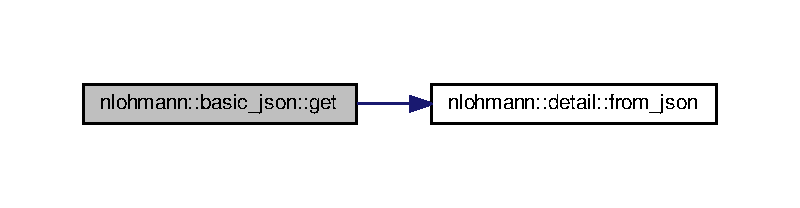
\includegraphics[width=350pt]{classnlohmann_1_1basic__json_a16f9445f7629f634221a42b967cdcd43_cgraph}
\end{center}
\end{figure}
\mbox{\Hypertarget{classnlohmann_1_1basic__json_ab728c42baff9d11409d4f99d9f95d6af}\label{classnlohmann_1_1basic__json_ab728c42baff9d11409d4f99d9f95d6af}} 
\index{nlohmann\+::basic\+\_\+json@{nlohmann\+::basic\+\_\+json}!get@{get}}
\index{get@{get}!nlohmann\+::basic\+\_\+json@{nlohmann\+::basic\+\_\+json}}
\subsubsection{\texorpdfstring{get()}{get()}\hspace{0.1cm}{\footnotesize\ttfamily [3/5]}}
{\footnotesize\ttfamily template$<$template$<$ typename U, typename V, typename... Args $>$ class Object\+Type = std\+::map, template$<$ typename U, typename... Args $>$ class Array\+Type = std\+::vector, class String\+Type  = std\+::string, class Boolean\+Type  = bool, class Number\+Integer\+Type  = std\+::int64\+\_\+t, class Number\+Unsigned\+Type  = std\+::uint64\+\_\+t, class Number\+Float\+Type  = double, template$<$ typename U $>$ class Allocator\+Type = std\+::allocator, template$<$ typename T, typename S\+F\+I\+N\+A\+E=void $>$ class J\+S\+O\+N\+Serializer = adl\+\_\+serializer$>$ \\
template$<$typename Value\+Type\+CV , typename Value\+Type  = detail\+::uncvref\+\_\+t$<$\+Value\+Type\+C\+V$>$, detail\+::enable\+\_\+if\+\_\+t$<$ not std\+::is\+\_\+same$<$ basic\+\_\+json\+\_\+t, Value\+Type $>$\+::value and detail\+::has\+\_\+non\+\_\+default\+\_\+from\+\_\+json$<$ basic\+\_\+json\+\_\+t, Value\+Type $>$\+::value, int $>$  = 0$>$ \\
Value\+Type \hyperlink{classnlohmann_1_1basic__json}{nlohmann\+::basic\+\_\+json}$<$ Object\+Type, Array\+Type, String\+Type, Boolean\+Type, Number\+Integer\+Type, Number\+Unsigned\+Type, Number\+Float\+Type, Allocator\+Type, J\+S\+O\+N\+Serializer $>$\+::get (\begin{DoxyParamCaption}{ }\end{DoxyParamCaption}) const\hspace{0.3cm}{\ttfamily [inline]}, {\ttfamily [noexcept]}}



get a value (explicit); special case 

Explicit type conversion between the J\+S\+ON value and a compatible value which is {\bfseries not} \href{http://en.cppreference.com/w/cpp/concept/CopyConstructible}{\tt Copy\+Constructible} and {\bfseries not} \href{http://en.cppreference.com/w/cpp/concept/DefaultConstructible}{\tt Default\+Constructible}. The value is converted by calling the \hyperlink{classnlohmann_1_1basic__json_a7768841baaaa7a21098a401c932efaff}{json\+\_\+serializer$<$\+Value\+Type$>$} {\ttfamily \hyperlink{namespacenlohmann_1_1detail_a839b0ab50d2c9bce669068f56bc41202}{from\+\_\+json()}} method.

The function is equivalent to executing 
\begin{DoxyCode}
\textcolor{keywordflow}{return} \hyperlink{namespaceshaan97_1_1sync_a9e374973ba3aed17d32efd550318c94c}{JSONSerializer<ValueTypeCV>::from\_json}(*\textcolor{keyword}{this});
\end{DoxyCode}


This overloads is chosen if\+:
\begin{DoxyItemize}
\item {\itshape Value\+Type} is not \hyperlink{classnlohmann_1_1basic__json}{basic\+\_\+json} and
\item \hyperlink{classnlohmann_1_1basic__json_a7768841baaaa7a21098a401c932efaff}{json\+\_\+serializer$<$\+Value\+Type$>$} has a {\ttfamily \hyperlink{namespacenlohmann_1_1detail_a839b0ab50d2c9bce669068f56bc41202}{from\+\_\+json()}} method of the form {\ttfamily Value\+Type from\+\_\+json(const @ref \hyperlink{classnlohmann_1_1basic__json}{basic\+\_\+json}\&)}
\end{DoxyItemize}

\begin{DoxyNote}{Note}
If \hyperlink{classnlohmann_1_1basic__json_a7768841baaaa7a21098a401c932efaff}{json\+\_\+serializer$<$\+Value\+Type$>$} has both overloads of {\ttfamily \hyperlink{namespacenlohmann_1_1detail_a839b0ab50d2c9bce669068f56bc41202}{from\+\_\+json()}}, this one is chosen.
\end{DoxyNote}

\begin{DoxyTemplParams}{Template Parameters}
{\em Value\+Type\+CV} & the provided value type \\
\hline
{\em Value\+Type} & the returned value type\\
\hline
\end{DoxyTemplParams}
\begin{DoxyReturn}{Returns}
copy of the J\+S\+ON value, converted to {\itshape Value\+Type} 
\end{DoxyReturn}

\begin{DoxyExceptions}{Exceptions}
{\em what} & \hyperlink{classnlohmann_1_1basic__json_a7768841baaaa7a21098a401c932efaff}{json\+\_\+serializer$<$\+Value\+Type$>$} {\ttfamily \hyperlink{namespacenlohmann_1_1detail_a839b0ab50d2c9bce669068f56bc41202}{from\+\_\+json()}} method throws\\
\hline
\end{DoxyExceptions}
\begin{DoxySince}{Since}
version 2.\+1.\+0 
\end{DoxySince}
Here is the call graph for this function\+:\nopagebreak
\begin{figure}[H]
\begin{center}
\leavevmode
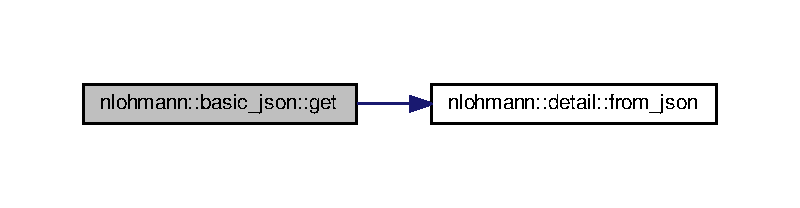
\includegraphics[width=350pt]{classnlohmann_1_1basic__json_ab728c42baff9d11409d4f99d9f95d6af_cgraph}
\end{center}
\end{figure}
\mbox{\Hypertarget{classnlohmann_1_1basic__json_a64135c19425f00b346d8ed63a23db334}\label{classnlohmann_1_1basic__json_a64135c19425f00b346d8ed63a23db334}} 
\index{nlohmann\+::basic\+\_\+json@{nlohmann\+::basic\+\_\+json}!get@{get}}
\index{get@{get}!nlohmann\+::basic\+\_\+json@{nlohmann\+::basic\+\_\+json}}
\subsubsection{\texorpdfstring{get()}{get()}\hspace{0.1cm}{\footnotesize\ttfamily [4/5]}}
{\footnotesize\ttfamily template$<$template$<$ typename U, typename V, typename... Args $>$ class Object\+Type = std\+::map, template$<$ typename U, typename... Args $>$ class Array\+Type = std\+::vector, class String\+Type  = std\+::string, class Boolean\+Type  = bool, class Number\+Integer\+Type  = std\+::int64\+\_\+t, class Number\+Unsigned\+Type  = std\+::uint64\+\_\+t, class Number\+Float\+Type  = double, template$<$ typename U $>$ class Allocator\+Type = std\+::allocator, template$<$ typename T, typename S\+F\+I\+N\+A\+E=void $>$ class J\+S\+O\+N\+Serializer = adl\+\_\+serializer$>$ \\
template$<$typename Pointer\+Type , typename std\+::enable\+\_\+if$<$ std\+::is\+\_\+pointer$<$ Pointer\+Type $>$\+::value, int $>$\+::type  = 0$>$ \\
Pointer\+Type \hyperlink{classnlohmann_1_1basic__json}{nlohmann\+::basic\+\_\+json}$<$ Object\+Type, Array\+Type, String\+Type, Boolean\+Type, Number\+Integer\+Type, Number\+Unsigned\+Type, Number\+Float\+Type, Allocator\+Type, J\+S\+O\+N\+Serializer $>$\+::get (\begin{DoxyParamCaption}{ }\end{DoxyParamCaption})\hspace{0.3cm}{\ttfamily [inline]}, {\ttfamily [noexcept]}}



get a pointer value (explicit) 

Explicit pointer access to the internally stored J\+S\+ON value. No copies are made.

\begin{DoxyWarning}{Warning}
The pointer becomes invalid if the underlying J\+S\+ON object changes.
\end{DoxyWarning}

\begin{DoxyTemplParams}{Template Parameters}
{\em Pointer\+Type} & pointer type; must be a pointer to \hyperlink{classnlohmann_1_1basic__json_ae095578e03df97c5b3991787f1056374}{array\+\_\+t}, \hyperlink{classnlohmann_1_1basic__json_aa1eb13d5aa86f80cbee6c58e90fbaf49}{object\+\_\+t}, \hyperlink{classnlohmann_1_1basic__json_a61f8566a1a85a424c7266fb531dca005}{string\+\_\+t}, \hyperlink{classnlohmann_1_1basic__json_a4c919102a9b4fe0d588af64801436082}{boolean\+\_\+t}, \hyperlink{classnlohmann_1_1basic__json_a98e611d67b7bd75307de99c9358ab2dc}{number\+\_\+integer\+\_\+t}, \hyperlink{classnlohmann_1_1basic__json_ab906e29b5d83ac162e823ada2156b989}{number\+\_\+unsigned\+\_\+t}, or \hyperlink{classnlohmann_1_1basic__json_a88d6103cb3620410b35200ee8e313d97}{number\+\_\+float\+\_\+t}.\\
\hline
\end{DoxyTemplParams}
\begin{DoxyReturn}{Returns}
pointer to the internally stored J\+S\+ON value if the requested pointer type {\itshape Pointer\+Type} fits to the J\+S\+ON value; {\ttfamily nullptr} otherwise
\end{DoxyReturn}
Constant.

\{The example below shows how pointers to internal values of a J\+S\+ON value can be requested. Note that no type conversions are made and a {\ttfamily nullptr} is returned if the value and the requested pointer type does not match.,get\+\_\+\+\_\+\+Pointer\+Type\}

\begin{DoxySeeAlso}{See also}
\hyperlink{classnlohmann_1_1basic__json_aefa46bd2d96bb77a38d1c8b431eab44f}{get\+\_\+ptr()} for explicit pointer-\/member access
\end{DoxySeeAlso}
\begin{DoxySince}{Since}
version 1.\+0.\+0 
\end{DoxySince}
\mbox{\Hypertarget{classnlohmann_1_1basic__json_a44a090c15a67b9f02e579b6e17ef0e1b}\label{classnlohmann_1_1basic__json_a44a090c15a67b9f02e579b6e17ef0e1b}} 
\index{nlohmann\+::basic\+\_\+json@{nlohmann\+::basic\+\_\+json}!get@{get}}
\index{get@{get}!nlohmann\+::basic\+\_\+json@{nlohmann\+::basic\+\_\+json}}
\subsubsection{\texorpdfstring{get()}{get()}\hspace{0.1cm}{\footnotesize\ttfamily [5/5]}}
{\footnotesize\ttfamily template$<$template$<$ typename U, typename V, typename... Args $>$ class Object\+Type = std\+::map, template$<$ typename U, typename... Args $>$ class Array\+Type = std\+::vector, class String\+Type  = std\+::string, class Boolean\+Type  = bool, class Number\+Integer\+Type  = std\+::int64\+\_\+t, class Number\+Unsigned\+Type  = std\+::uint64\+\_\+t, class Number\+Float\+Type  = double, template$<$ typename U $>$ class Allocator\+Type = std\+::allocator, template$<$ typename T, typename S\+F\+I\+N\+A\+E=void $>$ class J\+S\+O\+N\+Serializer = adl\+\_\+serializer$>$ \\
template$<$typename Pointer\+Type , typename std\+::enable\+\_\+if$<$ std\+::is\+\_\+pointer$<$ Pointer\+Type $>$\+::value, int $>$\+::type  = 0$>$ \\
constexpr const Pointer\+Type \hyperlink{classnlohmann_1_1basic__json}{nlohmann\+::basic\+\_\+json}$<$ Object\+Type, Array\+Type, String\+Type, Boolean\+Type, Number\+Integer\+Type, Number\+Unsigned\+Type, Number\+Float\+Type, Allocator\+Type, J\+S\+O\+N\+Serializer $>$\+::get (\begin{DoxyParamCaption}{ }\end{DoxyParamCaption}) const\hspace{0.3cm}{\ttfamily [inline]}, {\ttfamily [noexcept]}}



get a pointer value (explicit) 

get a pointer value (explicit) Explicit pointer access to the internally stored J\+S\+ON value. No copies are made.

\begin{DoxyWarning}{Warning}
The pointer becomes invalid if the underlying J\+S\+ON object changes.
\end{DoxyWarning}

\begin{DoxyTemplParams}{Template Parameters}
{\em Pointer\+Type} & pointer type; must be a pointer to \hyperlink{classnlohmann_1_1basic__json_ae095578e03df97c5b3991787f1056374}{array\+\_\+t}, \hyperlink{classnlohmann_1_1basic__json_aa1eb13d5aa86f80cbee6c58e90fbaf49}{object\+\_\+t}, \hyperlink{classnlohmann_1_1basic__json_a61f8566a1a85a424c7266fb531dca005}{string\+\_\+t}, \hyperlink{classnlohmann_1_1basic__json_a4c919102a9b4fe0d588af64801436082}{boolean\+\_\+t}, \hyperlink{classnlohmann_1_1basic__json_a98e611d67b7bd75307de99c9358ab2dc}{number\+\_\+integer\+\_\+t}, \hyperlink{classnlohmann_1_1basic__json_ab906e29b5d83ac162e823ada2156b989}{number\+\_\+unsigned\+\_\+t}, or \hyperlink{classnlohmann_1_1basic__json_a88d6103cb3620410b35200ee8e313d97}{number\+\_\+float\+\_\+t}.\\
\hline
\end{DoxyTemplParams}
\begin{DoxyReturn}{Returns}
pointer to the internally stored J\+S\+ON value if the requested pointer type {\itshape Pointer\+Type} fits to the J\+S\+ON value; {\ttfamily nullptr} otherwise
\end{DoxyReturn}
Constant.

\{The example below shows how pointers to internal values of a J\+S\+ON value can be requested. Note that no type conversions are made and a {\ttfamily nullptr} is returned if the value and the requested pointer type does not match.,get\+\_\+\+\_\+\+Pointer\+Type\}

\begin{DoxySeeAlso}{See also}
\hyperlink{classnlohmann_1_1basic__json_aefa46bd2d96bb77a38d1c8b431eab44f}{get\+\_\+ptr()} for explicit pointer-\/member access
\end{DoxySeeAlso}
\begin{DoxySince}{Since}
version 1.\+0.\+0 
\end{DoxySince}
\mbox{\Hypertarget{classnlohmann_1_1basic__json_af4ac14224fbdd29d3547fcb11bb55c8f}\label{classnlohmann_1_1basic__json_af4ac14224fbdd29d3547fcb11bb55c8f}} 
\index{nlohmann\+::basic\+\_\+json@{nlohmann\+::basic\+\_\+json}!get\+\_\+allocator@{get\+\_\+allocator}}
\index{get\+\_\+allocator@{get\+\_\+allocator}!nlohmann\+::basic\+\_\+json@{nlohmann\+::basic\+\_\+json}}
\subsubsection{\texorpdfstring{get\+\_\+allocator()}{get\_allocator()}}
{\footnotesize\ttfamily template$<$template$<$ typename U, typename V, typename... Args $>$ class Object\+Type = std\+::map, template$<$ typename U, typename... Args $>$ class Array\+Type = std\+::vector, class String\+Type  = std\+::string, class Boolean\+Type  = bool, class Number\+Integer\+Type  = std\+::int64\+\_\+t, class Number\+Unsigned\+Type  = std\+::uint64\+\_\+t, class Number\+Float\+Type  = double, template$<$ typename U $>$ class Allocator\+Type = std\+::allocator, template$<$ typename T, typename S\+F\+I\+N\+A\+E=void $>$ class J\+S\+O\+N\+Serializer = adl\+\_\+serializer$>$ \\
static \hyperlink{classnlohmann_1_1basic__json_a86ce930490cf7773b26f5ef49c04a350}{allocator\+\_\+type} \hyperlink{classnlohmann_1_1basic__json}{nlohmann\+::basic\+\_\+json}$<$ Object\+Type, Array\+Type, String\+Type, Boolean\+Type, Number\+Integer\+Type, Number\+Unsigned\+Type, Number\+Float\+Type, Allocator\+Type, J\+S\+O\+N\+Serializer $>$\+::get\+\_\+allocator (\begin{DoxyParamCaption}{ }\end{DoxyParamCaption})\hspace{0.3cm}{\ttfamily [inline]}, {\ttfamily [static]}}



returns the allocator associated with the container 

\mbox{\Hypertarget{classnlohmann_1_1basic__json_a12ecf6c70e147e27ccb24746a50dba57}\label{classnlohmann_1_1basic__json_a12ecf6c70e147e27ccb24746a50dba57}} 
\index{nlohmann\+::basic\+\_\+json@{nlohmann\+::basic\+\_\+json}!get\+\_\+from\+\_\+vector@{get\+\_\+from\+\_\+vector}}
\index{get\+\_\+from\+\_\+vector@{get\+\_\+from\+\_\+vector}!nlohmann\+::basic\+\_\+json@{nlohmann\+::basic\+\_\+json}}
\subsubsection{\texorpdfstring{get\+\_\+from\+\_\+vector()}{get\_from\_vector()}}
{\footnotesize\ttfamily template$<$template$<$ typename U, typename V, typename... Args $>$ class Object\+Type = std\+::map, template$<$ typename U, typename... Args $>$ class Array\+Type = std\+::vector, class String\+Type  = std\+::string, class Boolean\+Type  = bool, class Number\+Integer\+Type  = std\+::int64\+\_\+t, class Number\+Unsigned\+Type  = std\+::uint64\+\_\+t, class Number\+Float\+Type  = double, template$<$ typename U $>$ class Allocator\+Type = std\+::allocator, template$<$ typename T, typename S\+F\+I\+N\+A\+E=void $>$ class J\+S\+O\+N\+Serializer = adl\+\_\+serializer$>$ \\
template$<$typename T $>$ \\
static T \hyperlink{classnlohmann_1_1basic__json}{nlohmann\+::basic\+\_\+json}$<$ Object\+Type, Array\+Type, String\+Type, Boolean\+Type, Number\+Integer\+Type, Number\+Unsigned\+Type, Number\+Float\+Type, Allocator\+Type, J\+S\+O\+N\+Serializer $>$\+::get\+\_\+from\+\_\+vector (\begin{DoxyParamCaption}\item[{const std\+::vector$<$ uint8\+\_\+t $>$ \&}]{vec,  }\item[{const size\+\_\+t}]{current\+\_\+index }\end{DoxyParamCaption})\hspace{0.3cm}{\ttfamily [inline]}, {\ttfamily [static]}, {\ttfamily [private]}}



take sufficient bytes from a vector to fill an integer variable 

In the context of binary serialization formats, we need to read several bytes from a byte vector and combine them to multi-\/byte integral data types.


\begin{DoxyParams}[1]{Parameters}
\mbox{\tt in}  & {\em vec} & byte vector to read from \\
\hline
\mbox{\tt in}  & {\em current\+\_\+index} & the position in the vector after which to read\\
\hline
\end{DoxyParams}
\begin{DoxyReturn}{Returns}
the next sizeof(\+T) bytes from {\itshape vec}, in reverse order as T
\end{DoxyReturn}

\begin{DoxyTemplParams}{Template Parameters}
{\em T} & the integral return type\\
\hline
\end{DoxyTemplParams}

\begin{DoxyExceptions}{Exceptions}
{\em std\+::out\+\_\+of\+\_\+range} & if there are less than sizeof(\+T)+1 bytes in the vector {\itshape vec} to read\\
\hline
\end{DoxyExceptions}
In the for loop, the bytes from the vector are copied in reverse order into the return value. In the figures below, let sizeof(\+T)=4 and {\ttfamily i} be the loop variable.

Precondition\+:

vec\+: $\vert$ $\vert$ $\vert$ a $\vert$ b $\vert$ c $\vert$ d $\vert$ T\+: $\vert$ $\vert$ $\vert$ $\vert$ $\vert$ $^\wedge$ $^\wedge$ $^\wedge$ $^\wedge$ current\+\_\+index i ptr sizeof(\+T)

Postcondition\+:

vec\+: $\vert$ $\vert$ $\vert$ a $\vert$ b $\vert$ c $\vert$ d $\vert$ T\+: $\vert$ d $\vert$ c $\vert$ b $\vert$ a $\vert$ $^\wedge$ $^\wedge$ $^\wedge$ $\vert$ i ptr current\+\_\+index

\begin{DoxySeeAlso}{See also}
Code adapted from \href{http://stackoverflow.com/a/41031865/266378}{\tt http\+://stackoverflow.\+com/a/41031865/266378}. 
\end{DoxySeeAlso}
\mbox{\Hypertarget{classnlohmann_1_1basic__json_ac686d87a2261f85f1df97035b14a6e3a}\label{classnlohmann_1_1basic__json_ac686d87a2261f85f1df97035b14a6e3a}} 
\index{nlohmann\+::basic\+\_\+json@{nlohmann\+::basic\+\_\+json}!get\+\_\+impl@{get\+\_\+impl}}
\index{get\+\_\+impl@{get\+\_\+impl}!nlohmann\+::basic\+\_\+json@{nlohmann\+::basic\+\_\+json}}
\subsubsection{\texorpdfstring{get\+\_\+impl()}{get\_impl()}}
{\footnotesize\ttfamily template$<$template$<$ typename U, typename V, typename... Args $>$ class Object\+Type = std\+::map, template$<$ typename U, typename... Args $>$ class Array\+Type = std\+::vector, class String\+Type  = std\+::string, class Boolean\+Type  = bool, class Number\+Integer\+Type  = std\+::int64\+\_\+t, class Number\+Unsigned\+Type  = std\+::uint64\+\_\+t, class Number\+Float\+Type  = double, template$<$ typename U $>$ class Allocator\+Type = std\+::allocator, template$<$ typename T, typename S\+F\+I\+N\+A\+E=void $>$ class J\+S\+O\+N\+Serializer = adl\+\_\+serializer$>$ \\
\hyperlink{classnlohmann_1_1basic__json_a4c919102a9b4fe0d588af64801436082}{boolean\+\_\+t} \hyperlink{classnlohmann_1_1basic__json}{nlohmann\+::basic\+\_\+json}$<$ Object\+Type, Array\+Type, String\+Type, Boolean\+Type, Number\+Integer\+Type, Number\+Unsigned\+Type, Number\+Float\+Type, Allocator\+Type, J\+S\+O\+N\+Serializer $>$\+::get\+\_\+impl (\begin{DoxyParamCaption}\item[{\hyperlink{classnlohmann_1_1basic__json_a4c919102a9b4fe0d588af64801436082}{boolean\+\_\+t} $\ast$}]{ }\end{DoxyParamCaption}) const\hspace{0.3cm}{\ttfamily [inline]}, {\ttfamily [private]}}



get a boolean (explicit) 

\mbox{\Hypertarget{classnlohmann_1_1basic__json_a58b65f595883fb93333423ec5e3bafee}\label{classnlohmann_1_1basic__json_a58b65f595883fb93333423ec5e3bafee}} 
\index{nlohmann\+::basic\+\_\+json@{nlohmann\+::basic\+\_\+json}!get\+\_\+impl\+\_\+ptr@{get\+\_\+impl\+\_\+ptr}}
\index{get\+\_\+impl\+\_\+ptr@{get\+\_\+impl\+\_\+ptr}!nlohmann\+::basic\+\_\+json@{nlohmann\+::basic\+\_\+json}}
\subsubsection{\texorpdfstring{get\+\_\+impl\+\_\+ptr()}{get\_impl\_ptr()}\hspace{0.1cm}{\footnotesize\ttfamily [1/14]}}
{\footnotesize\ttfamily template$<$template$<$ typename U, typename V, typename... Args $>$ class Object\+Type = std\+::map, template$<$ typename U, typename... Args $>$ class Array\+Type = std\+::vector, class String\+Type  = std\+::string, class Boolean\+Type  = bool, class Number\+Integer\+Type  = std\+::int64\+\_\+t, class Number\+Unsigned\+Type  = std\+::uint64\+\_\+t, class Number\+Float\+Type  = double, template$<$ typename U $>$ class Allocator\+Type = std\+::allocator, template$<$ typename T, typename S\+F\+I\+N\+A\+E=void $>$ class J\+S\+O\+N\+Serializer = adl\+\_\+serializer$>$ \\
\hyperlink{classnlohmann_1_1basic__json_aa1eb13d5aa86f80cbee6c58e90fbaf49}{object\+\_\+t}$\ast$ \hyperlink{classnlohmann_1_1basic__json}{nlohmann\+::basic\+\_\+json}$<$ Object\+Type, Array\+Type, String\+Type, Boolean\+Type, Number\+Integer\+Type, Number\+Unsigned\+Type, Number\+Float\+Type, Allocator\+Type, J\+S\+O\+N\+Serializer $>$\+::get\+\_\+impl\+\_\+ptr (\begin{DoxyParamCaption}\item[{\hyperlink{classnlohmann_1_1basic__json_aa1eb13d5aa86f80cbee6c58e90fbaf49}{object\+\_\+t} $\ast$}]{ }\end{DoxyParamCaption})\hspace{0.3cm}{\ttfamily [inline]}, {\ttfamily [private]}, {\ttfamily [noexcept]}}



get a pointer to the value (object) 

\mbox{\Hypertarget{classnlohmann_1_1basic__json_aff66aa31ef8603d799433b26fe7535c9}\label{classnlohmann_1_1basic__json_aff66aa31ef8603d799433b26fe7535c9}} 
\index{nlohmann\+::basic\+\_\+json@{nlohmann\+::basic\+\_\+json}!get\+\_\+impl\+\_\+ptr@{get\+\_\+impl\+\_\+ptr}}
\index{get\+\_\+impl\+\_\+ptr@{get\+\_\+impl\+\_\+ptr}!nlohmann\+::basic\+\_\+json@{nlohmann\+::basic\+\_\+json}}
\subsubsection{\texorpdfstring{get\+\_\+impl\+\_\+ptr()}{get\_impl\_ptr()}\hspace{0.1cm}{\footnotesize\ttfamily [2/14]}}
{\footnotesize\ttfamily template$<$template$<$ typename U, typename V, typename... Args $>$ class Object\+Type = std\+::map, template$<$ typename U, typename... Args $>$ class Array\+Type = std\+::vector, class String\+Type  = std\+::string, class Boolean\+Type  = bool, class Number\+Integer\+Type  = std\+::int64\+\_\+t, class Number\+Unsigned\+Type  = std\+::uint64\+\_\+t, class Number\+Float\+Type  = double, template$<$ typename U $>$ class Allocator\+Type = std\+::allocator, template$<$ typename T, typename S\+F\+I\+N\+A\+E=void $>$ class J\+S\+O\+N\+Serializer = adl\+\_\+serializer$>$ \\
constexpr const \hyperlink{classnlohmann_1_1basic__json_aa1eb13d5aa86f80cbee6c58e90fbaf49}{object\+\_\+t}$\ast$ \hyperlink{classnlohmann_1_1basic__json}{nlohmann\+::basic\+\_\+json}$<$ Object\+Type, Array\+Type, String\+Type, Boolean\+Type, Number\+Integer\+Type, Number\+Unsigned\+Type, Number\+Float\+Type, Allocator\+Type, J\+S\+O\+N\+Serializer $>$\+::get\+\_\+impl\+\_\+ptr (\begin{DoxyParamCaption}\item[{const \hyperlink{classnlohmann_1_1basic__json_aa1eb13d5aa86f80cbee6c58e90fbaf49}{object\+\_\+t} $\ast$}]{ }\end{DoxyParamCaption}) const\hspace{0.3cm}{\ttfamily [inline]}, {\ttfamily [private]}, {\ttfamily [noexcept]}}



get a pointer to the value (object) 

\mbox{\Hypertarget{classnlohmann_1_1basic__json_a0a9c36d4d94ef5d611c0204bc7e4d37f}\label{classnlohmann_1_1basic__json_a0a9c36d4d94ef5d611c0204bc7e4d37f}} 
\index{nlohmann\+::basic\+\_\+json@{nlohmann\+::basic\+\_\+json}!get\+\_\+impl\+\_\+ptr@{get\+\_\+impl\+\_\+ptr}}
\index{get\+\_\+impl\+\_\+ptr@{get\+\_\+impl\+\_\+ptr}!nlohmann\+::basic\+\_\+json@{nlohmann\+::basic\+\_\+json}}
\subsubsection{\texorpdfstring{get\+\_\+impl\+\_\+ptr()}{get\_impl\_ptr()}\hspace{0.1cm}{\footnotesize\ttfamily [3/14]}}
{\footnotesize\ttfamily template$<$template$<$ typename U, typename V, typename... Args $>$ class Object\+Type = std\+::map, template$<$ typename U, typename... Args $>$ class Array\+Type = std\+::vector, class String\+Type  = std\+::string, class Boolean\+Type  = bool, class Number\+Integer\+Type  = std\+::int64\+\_\+t, class Number\+Unsigned\+Type  = std\+::uint64\+\_\+t, class Number\+Float\+Type  = double, template$<$ typename U $>$ class Allocator\+Type = std\+::allocator, template$<$ typename T, typename S\+F\+I\+N\+A\+E=void $>$ class J\+S\+O\+N\+Serializer = adl\+\_\+serializer$>$ \\
\hyperlink{classnlohmann_1_1basic__json_ae095578e03df97c5b3991787f1056374}{array\+\_\+t}$\ast$ \hyperlink{classnlohmann_1_1basic__json}{nlohmann\+::basic\+\_\+json}$<$ Object\+Type, Array\+Type, String\+Type, Boolean\+Type, Number\+Integer\+Type, Number\+Unsigned\+Type, Number\+Float\+Type, Allocator\+Type, J\+S\+O\+N\+Serializer $>$\+::get\+\_\+impl\+\_\+ptr (\begin{DoxyParamCaption}\item[{\hyperlink{classnlohmann_1_1basic__json_ae095578e03df97c5b3991787f1056374}{array\+\_\+t} $\ast$}]{ }\end{DoxyParamCaption})\hspace{0.3cm}{\ttfamily [inline]}, {\ttfamily [private]}, {\ttfamily [noexcept]}}



get a pointer to the value (array) 

\mbox{\Hypertarget{classnlohmann_1_1basic__json_abefb50a81c9b91106d9ecadfcd1ee2b5}\label{classnlohmann_1_1basic__json_abefb50a81c9b91106d9ecadfcd1ee2b5}} 
\index{nlohmann\+::basic\+\_\+json@{nlohmann\+::basic\+\_\+json}!get\+\_\+impl\+\_\+ptr@{get\+\_\+impl\+\_\+ptr}}
\index{get\+\_\+impl\+\_\+ptr@{get\+\_\+impl\+\_\+ptr}!nlohmann\+::basic\+\_\+json@{nlohmann\+::basic\+\_\+json}}
\subsubsection{\texorpdfstring{get\+\_\+impl\+\_\+ptr()}{get\_impl\_ptr()}\hspace{0.1cm}{\footnotesize\ttfamily [4/14]}}
{\footnotesize\ttfamily template$<$template$<$ typename U, typename V, typename... Args $>$ class Object\+Type = std\+::map, template$<$ typename U, typename... Args $>$ class Array\+Type = std\+::vector, class String\+Type  = std\+::string, class Boolean\+Type  = bool, class Number\+Integer\+Type  = std\+::int64\+\_\+t, class Number\+Unsigned\+Type  = std\+::uint64\+\_\+t, class Number\+Float\+Type  = double, template$<$ typename U $>$ class Allocator\+Type = std\+::allocator, template$<$ typename T, typename S\+F\+I\+N\+A\+E=void $>$ class J\+S\+O\+N\+Serializer = adl\+\_\+serializer$>$ \\
constexpr const \hyperlink{classnlohmann_1_1basic__json_ae095578e03df97c5b3991787f1056374}{array\+\_\+t}$\ast$ \hyperlink{classnlohmann_1_1basic__json}{nlohmann\+::basic\+\_\+json}$<$ Object\+Type, Array\+Type, String\+Type, Boolean\+Type, Number\+Integer\+Type, Number\+Unsigned\+Type, Number\+Float\+Type, Allocator\+Type, J\+S\+O\+N\+Serializer $>$\+::get\+\_\+impl\+\_\+ptr (\begin{DoxyParamCaption}\item[{const \hyperlink{classnlohmann_1_1basic__json_ae095578e03df97c5b3991787f1056374}{array\+\_\+t} $\ast$}]{ }\end{DoxyParamCaption}) const\hspace{0.3cm}{\ttfamily [inline]}, {\ttfamily [private]}, {\ttfamily [noexcept]}}



get a pointer to the value (array) 

\mbox{\Hypertarget{classnlohmann_1_1basic__json_a955d7098e5b43ee0dd8cce5f707eeb5c}\label{classnlohmann_1_1basic__json_a955d7098e5b43ee0dd8cce5f707eeb5c}} 
\index{nlohmann\+::basic\+\_\+json@{nlohmann\+::basic\+\_\+json}!get\+\_\+impl\+\_\+ptr@{get\+\_\+impl\+\_\+ptr}}
\index{get\+\_\+impl\+\_\+ptr@{get\+\_\+impl\+\_\+ptr}!nlohmann\+::basic\+\_\+json@{nlohmann\+::basic\+\_\+json}}
\subsubsection{\texorpdfstring{get\+\_\+impl\+\_\+ptr()}{get\_impl\_ptr()}\hspace{0.1cm}{\footnotesize\ttfamily [5/14]}}
{\footnotesize\ttfamily template$<$template$<$ typename U, typename V, typename... Args $>$ class Object\+Type = std\+::map, template$<$ typename U, typename... Args $>$ class Array\+Type = std\+::vector, class String\+Type  = std\+::string, class Boolean\+Type  = bool, class Number\+Integer\+Type  = std\+::int64\+\_\+t, class Number\+Unsigned\+Type  = std\+::uint64\+\_\+t, class Number\+Float\+Type  = double, template$<$ typename U $>$ class Allocator\+Type = std\+::allocator, template$<$ typename T, typename S\+F\+I\+N\+A\+E=void $>$ class J\+S\+O\+N\+Serializer = adl\+\_\+serializer$>$ \\
\hyperlink{classnlohmann_1_1basic__json_a61f8566a1a85a424c7266fb531dca005}{string\+\_\+t}$\ast$ \hyperlink{classnlohmann_1_1basic__json}{nlohmann\+::basic\+\_\+json}$<$ Object\+Type, Array\+Type, String\+Type, Boolean\+Type, Number\+Integer\+Type, Number\+Unsigned\+Type, Number\+Float\+Type, Allocator\+Type, J\+S\+O\+N\+Serializer $>$\+::get\+\_\+impl\+\_\+ptr (\begin{DoxyParamCaption}\item[{\hyperlink{classnlohmann_1_1basic__json_a61f8566a1a85a424c7266fb531dca005}{string\+\_\+t} $\ast$}]{ }\end{DoxyParamCaption})\hspace{0.3cm}{\ttfamily [inline]}, {\ttfamily [private]}, {\ttfamily [noexcept]}}



get a pointer to the value (string) 

\mbox{\Hypertarget{classnlohmann_1_1basic__json_a0c0b516e06d10dced993934ba5139cc0}\label{classnlohmann_1_1basic__json_a0c0b516e06d10dced993934ba5139cc0}} 
\index{nlohmann\+::basic\+\_\+json@{nlohmann\+::basic\+\_\+json}!get\+\_\+impl\+\_\+ptr@{get\+\_\+impl\+\_\+ptr}}
\index{get\+\_\+impl\+\_\+ptr@{get\+\_\+impl\+\_\+ptr}!nlohmann\+::basic\+\_\+json@{nlohmann\+::basic\+\_\+json}}
\subsubsection{\texorpdfstring{get\+\_\+impl\+\_\+ptr()}{get\_impl\_ptr()}\hspace{0.1cm}{\footnotesize\ttfamily [6/14]}}
{\footnotesize\ttfamily template$<$template$<$ typename U, typename V, typename... Args $>$ class Object\+Type = std\+::map, template$<$ typename U, typename... Args $>$ class Array\+Type = std\+::vector, class String\+Type  = std\+::string, class Boolean\+Type  = bool, class Number\+Integer\+Type  = std\+::int64\+\_\+t, class Number\+Unsigned\+Type  = std\+::uint64\+\_\+t, class Number\+Float\+Type  = double, template$<$ typename U $>$ class Allocator\+Type = std\+::allocator, template$<$ typename T, typename S\+F\+I\+N\+A\+E=void $>$ class J\+S\+O\+N\+Serializer = adl\+\_\+serializer$>$ \\
constexpr const \hyperlink{classnlohmann_1_1basic__json_a61f8566a1a85a424c7266fb531dca005}{string\+\_\+t}$\ast$ \hyperlink{classnlohmann_1_1basic__json}{nlohmann\+::basic\+\_\+json}$<$ Object\+Type, Array\+Type, String\+Type, Boolean\+Type, Number\+Integer\+Type, Number\+Unsigned\+Type, Number\+Float\+Type, Allocator\+Type, J\+S\+O\+N\+Serializer $>$\+::get\+\_\+impl\+\_\+ptr (\begin{DoxyParamCaption}\item[{const \hyperlink{classnlohmann_1_1basic__json_a61f8566a1a85a424c7266fb531dca005}{string\+\_\+t} $\ast$}]{ }\end{DoxyParamCaption}) const\hspace{0.3cm}{\ttfamily [inline]}, {\ttfamily [private]}, {\ttfamily [noexcept]}}



get a pointer to the value (string) 

\mbox{\Hypertarget{classnlohmann_1_1basic__json_ab1678fb6723faf020a15300c4f6b98f5}\label{classnlohmann_1_1basic__json_ab1678fb6723faf020a15300c4f6b98f5}} 
\index{nlohmann\+::basic\+\_\+json@{nlohmann\+::basic\+\_\+json}!get\+\_\+impl\+\_\+ptr@{get\+\_\+impl\+\_\+ptr}}
\index{get\+\_\+impl\+\_\+ptr@{get\+\_\+impl\+\_\+ptr}!nlohmann\+::basic\+\_\+json@{nlohmann\+::basic\+\_\+json}}
\subsubsection{\texorpdfstring{get\+\_\+impl\+\_\+ptr()}{get\_impl\_ptr()}\hspace{0.1cm}{\footnotesize\ttfamily [7/14]}}
{\footnotesize\ttfamily template$<$template$<$ typename U, typename V, typename... Args $>$ class Object\+Type = std\+::map, template$<$ typename U, typename... Args $>$ class Array\+Type = std\+::vector, class String\+Type  = std\+::string, class Boolean\+Type  = bool, class Number\+Integer\+Type  = std\+::int64\+\_\+t, class Number\+Unsigned\+Type  = std\+::uint64\+\_\+t, class Number\+Float\+Type  = double, template$<$ typename U $>$ class Allocator\+Type = std\+::allocator, template$<$ typename T, typename S\+F\+I\+N\+A\+E=void $>$ class J\+S\+O\+N\+Serializer = adl\+\_\+serializer$>$ \\
\hyperlink{classnlohmann_1_1basic__json_a4c919102a9b4fe0d588af64801436082}{boolean\+\_\+t}$\ast$ \hyperlink{classnlohmann_1_1basic__json}{nlohmann\+::basic\+\_\+json}$<$ Object\+Type, Array\+Type, String\+Type, Boolean\+Type, Number\+Integer\+Type, Number\+Unsigned\+Type, Number\+Float\+Type, Allocator\+Type, J\+S\+O\+N\+Serializer $>$\+::get\+\_\+impl\+\_\+ptr (\begin{DoxyParamCaption}\item[{\hyperlink{classnlohmann_1_1basic__json_a4c919102a9b4fe0d588af64801436082}{boolean\+\_\+t} $\ast$}]{ }\end{DoxyParamCaption})\hspace{0.3cm}{\ttfamily [inline]}, {\ttfamily [private]}, {\ttfamily [noexcept]}}



get a pointer to the value (boolean) 

\mbox{\Hypertarget{classnlohmann_1_1basic__json_ae068eee75c0a814e19208bae641f866c}\label{classnlohmann_1_1basic__json_ae068eee75c0a814e19208bae641f866c}} 
\index{nlohmann\+::basic\+\_\+json@{nlohmann\+::basic\+\_\+json}!get\+\_\+impl\+\_\+ptr@{get\+\_\+impl\+\_\+ptr}}
\index{get\+\_\+impl\+\_\+ptr@{get\+\_\+impl\+\_\+ptr}!nlohmann\+::basic\+\_\+json@{nlohmann\+::basic\+\_\+json}}
\subsubsection{\texorpdfstring{get\+\_\+impl\+\_\+ptr()}{get\_impl\_ptr()}\hspace{0.1cm}{\footnotesize\ttfamily [8/14]}}
{\footnotesize\ttfamily template$<$template$<$ typename U, typename V, typename... Args $>$ class Object\+Type = std\+::map, template$<$ typename U, typename... Args $>$ class Array\+Type = std\+::vector, class String\+Type  = std\+::string, class Boolean\+Type  = bool, class Number\+Integer\+Type  = std\+::int64\+\_\+t, class Number\+Unsigned\+Type  = std\+::uint64\+\_\+t, class Number\+Float\+Type  = double, template$<$ typename U $>$ class Allocator\+Type = std\+::allocator, template$<$ typename T, typename S\+F\+I\+N\+A\+E=void $>$ class J\+S\+O\+N\+Serializer = adl\+\_\+serializer$>$ \\
constexpr const \hyperlink{classnlohmann_1_1basic__json_a4c919102a9b4fe0d588af64801436082}{boolean\+\_\+t}$\ast$ \hyperlink{classnlohmann_1_1basic__json}{nlohmann\+::basic\+\_\+json}$<$ Object\+Type, Array\+Type, String\+Type, Boolean\+Type, Number\+Integer\+Type, Number\+Unsigned\+Type, Number\+Float\+Type, Allocator\+Type, J\+S\+O\+N\+Serializer $>$\+::get\+\_\+impl\+\_\+ptr (\begin{DoxyParamCaption}\item[{const \hyperlink{classnlohmann_1_1basic__json_a4c919102a9b4fe0d588af64801436082}{boolean\+\_\+t} $\ast$}]{ }\end{DoxyParamCaption}) const\hspace{0.3cm}{\ttfamily [inline]}, {\ttfamily [private]}, {\ttfamily [noexcept]}}



get a pointer to the value (boolean) 

\mbox{\Hypertarget{classnlohmann_1_1basic__json_a32a4c3ccdd09b663614adce1834a0a50}\label{classnlohmann_1_1basic__json_a32a4c3ccdd09b663614adce1834a0a50}} 
\index{nlohmann\+::basic\+\_\+json@{nlohmann\+::basic\+\_\+json}!get\+\_\+impl\+\_\+ptr@{get\+\_\+impl\+\_\+ptr}}
\index{get\+\_\+impl\+\_\+ptr@{get\+\_\+impl\+\_\+ptr}!nlohmann\+::basic\+\_\+json@{nlohmann\+::basic\+\_\+json}}
\subsubsection{\texorpdfstring{get\+\_\+impl\+\_\+ptr()}{get\_impl\_ptr()}\hspace{0.1cm}{\footnotesize\ttfamily [9/14]}}
{\footnotesize\ttfamily template$<$template$<$ typename U, typename V, typename... Args $>$ class Object\+Type = std\+::map, template$<$ typename U, typename... Args $>$ class Array\+Type = std\+::vector, class String\+Type  = std\+::string, class Boolean\+Type  = bool, class Number\+Integer\+Type  = std\+::int64\+\_\+t, class Number\+Unsigned\+Type  = std\+::uint64\+\_\+t, class Number\+Float\+Type  = double, template$<$ typename U $>$ class Allocator\+Type = std\+::allocator, template$<$ typename T, typename S\+F\+I\+N\+A\+E=void $>$ class J\+S\+O\+N\+Serializer = adl\+\_\+serializer$>$ \\
\hyperlink{classnlohmann_1_1basic__json_a98e611d67b7bd75307de99c9358ab2dc}{number\+\_\+integer\+\_\+t}$\ast$ \hyperlink{classnlohmann_1_1basic__json}{nlohmann\+::basic\+\_\+json}$<$ Object\+Type, Array\+Type, String\+Type, Boolean\+Type, Number\+Integer\+Type, Number\+Unsigned\+Type, Number\+Float\+Type, Allocator\+Type, J\+S\+O\+N\+Serializer $>$\+::get\+\_\+impl\+\_\+ptr (\begin{DoxyParamCaption}\item[{\hyperlink{classnlohmann_1_1basic__json_a98e611d67b7bd75307de99c9358ab2dc}{number\+\_\+integer\+\_\+t} $\ast$}]{ }\end{DoxyParamCaption})\hspace{0.3cm}{\ttfamily [inline]}, {\ttfamily [private]}, {\ttfamily [noexcept]}}



get a pointer to the value (integer number) 

\mbox{\Hypertarget{classnlohmann_1_1basic__json_a0a01103792cc54e9c8236361e5f7ed90}\label{classnlohmann_1_1basic__json_a0a01103792cc54e9c8236361e5f7ed90}} 
\index{nlohmann\+::basic\+\_\+json@{nlohmann\+::basic\+\_\+json}!get\+\_\+impl\+\_\+ptr@{get\+\_\+impl\+\_\+ptr}}
\index{get\+\_\+impl\+\_\+ptr@{get\+\_\+impl\+\_\+ptr}!nlohmann\+::basic\+\_\+json@{nlohmann\+::basic\+\_\+json}}
\subsubsection{\texorpdfstring{get\+\_\+impl\+\_\+ptr()}{get\_impl\_ptr()}\hspace{0.1cm}{\footnotesize\ttfamily [10/14]}}
{\footnotesize\ttfamily template$<$template$<$ typename U, typename V, typename... Args $>$ class Object\+Type = std\+::map, template$<$ typename U, typename... Args $>$ class Array\+Type = std\+::vector, class String\+Type  = std\+::string, class Boolean\+Type  = bool, class Number\+Integer\+Type  = std\+::int64\+\_\+t, class Number\+Unsigned\+Type  = std\+::uint64\+\_\+t, class Number\+Float\+Type  = double, template$<$ typename U $>$ class Allocator\+Type = std\+::allocator, template$<$ typename T, typename S\+F\+I\+N\+A\+E=void $>$ class J\+S\+O\+N\+Serializer = adl\+\_\+serializer$>$ \\
constexpr const \hyperlink{classnlohmann_1_1basic__json_a98e611d67b7bd75307de99c9358ab2dc}{number\+\_\+integer\+\_\+t}$\ast$ \hyperlink{classnlohmann_1_1basic__json}{nlohmann\+::basic\+\_\+json}$<$ Object\+Type, Array\+Type, String\+Type, Boolean\+Type, Number\+Integer\+Type, Number\+Unsigned\+Type, Number\+Float\+Type, Allocator\+Type, J\+S\+O\+N\+Serializer $>$\+::get\+\_\+impl\+\_\+ptr (\begin{DoxyParamCaption}\item[{const \hyperlink{classnlohmann_1_1basic__json_a98e611d67b7bd75307de99c9358ab2dc}{number\+\_\+integer\+\_\+t} $\ast$}]{ }\end{DoxyParamCaption}) const\hspace{0.3cm}{\ttfamily [inline]}, {\ttfamily [private]}, {\ttfamily [noexcept]}}



get a pointer to the value (integer number) 

\mbox{\Hypertarget{classnlohmann_1_1basic__json_aa9aaed6b92909b263e04b5d25eba8d67}\label{classnlohmann_1_1basic__json_aa9aaed6b92909b263e04b5d25eba8d67}} 
\index{nlohmann\+::basic\+\_\+json@{nlohmann\+::basic\+\_\+json}!get\+\_\+impl\+\_\+ptr@{get\+\_\+impl\+\_\+ptr}}
\index{get\+\_\+impl\+\_\+ptr@{get\+\_\+impl\+\_\+ptr}!nlohmann\+::basic\+\_\+json@{nlohmann\+::basic\+\_\+json}}
\subsubsection{\texorpdfstring{get\+\_\+impl\+\_\+ptr()}{get\_impl\_ptr()}\hspace{0.1cm}{\footnotesize\ttfamily [11/14]}}
{\footnotesize\ttfamily template$<$template$<$ typename U, typename V, typename... Args $>$ class Object\+Type = std\+::map, template$<$ typename U, typename... Args $>$ class Array\+Type = std\+::vector, class String\+Type  = std\+::string, class Boolean\+Type  = bool, class Number\+Integer\+Type  = std\+::int64\+\_\+t, class Number\+Unsigned\+Type  = std\+::uint64\+\_\+t, class Number\+Float\+Type  = double, template$<$ typename U $>$ class Allocator\+Type = std\+::allocator, template$<$ typename T, typename S\+F\+I\+N\+A\+E=void $>$ class J\+S\+O\+N\+Serializer = adl\+\_\+serializer$>$ \\
\hyperlink{classnlohmann_1_1basic__json_ab906e29b5d83ac162e823ada2156b989}{number\+\_\+unsigned\+\_\+t}$\ast$ \hyperlink{classnlohmann_1_1basic__json}{nlohmann\+::basic\+\_\+json}$<$ Object\+Type, Array\+Type, String\+Type, Boolean\+Type, Number\+Integer\+Type, Number\+Unsigned\+Type, Number\+Float\+Type, Allocator\+Type, J\+S\+O\+N\+Serializer $>$\+::get\+\_\+impl\+\_\+ptr (\begin{DoxyParamCaption}\item[{\hyperlink{classnlohmann_1_1basic__json_ab906e29b5d83ac162e823ada2156b989}{number\+\_\+unsigned\+\_\+t} $\ast$}]{ }\end{DoxyParamCaption})\hspace{0.3cm}{\ttfamily [inline]}, {\ttfamily [private]}, {\ttfamily [noexcept]}}



get a pointer to the value (unsigned number) 

\mbox{\Hypertarget{classnlohmann_1_1basic__json_a52d0c7f354c6155221540baef5b98d0a}\label{classnlohmann_1_1basic__json_a52d0c7f354c6155221540baef5b98d0a}} 
\index{nlohmann\+::basic\+\_\+json@{nlohmann\+::basic\+\_\+json}!get\+\_\+impl\+\_\+ptr@{get\+\_\+impl\+\_\+ptr}}
\index{get\+\_\+impl\+\_\+ptr@{get\+\_\+impl\+\_\+ptr}!nlohmann\+::basic\+\_\+json@{nlohmann\+::basic\+\_\+json}}
\subsubsection{\texorpdfstring{get\+\_\+impl\+\_\+ptr()}{get\_impl\_ptr()}\hspace{0.1cm}{\footnotesize\ttfamily [12/14]}}
{\footnotesize\ttfamily template$<$template$<$ typename U, typename V, typename... Args $>$ class Object\+Type = std\+::map, template$<$ typename U, typename... Args $>$ class Array\+Type = std\+::vector, class String\+Type  = std\+::string, class Boolean\+Type  = bool, class Number\+Integer\+Type  = std\+::int64\+\_\+t, class Number\+Unsigned\+Type  = std\+::uint64\+\_\+t, class Number\+Float\+Type  = double, template$<$ typename U $>$ class Allocator\+Type = std\+::allocator, template$<$ typename T, typename S\+F\+I\+N\+A\+E=void $>$ class J\+S\+O\+N\+Serializer = adl\+\_\+serializer$>$ \\
constexpr const \hyperlink{classnlohmann_1_1basic__json_ab906e29b5d83ac162e823ada2156b989}{number\+\_\+unsigned\+\_\+t}$\ast$ \hyperlink{classnlohmann_1_1basic__json}{nlohmann\+::basic\+\_\+json}$<$ Object\+Type, Array\+Type, String\+Type, Boolean\+Type, Number\+Integer\+Type, Number\+Unsigned\+Type, Number\+Float\+Type, Allocator\+Type, J\+S\+O\+N\+Serializer $>$\+::get\+\_\+impl\+\_\+ptr (\begin{DoxyParamCaption}\item[{const \hyperlink{classnlohmann_1_1basic__json_ab906e29b5d83ac162e823ada2156b989}{number\+\_\+unsigned\+\_\+t} $\ast$}]{ }\end{DoxyParamCaption}) const\hspace{0.3cm}{\ttfamily [inline]}, {\ttfamily [private]}, {\ttfamily [noexcept]}}



get a pointer to the value (unsigned number) 

\mbox{\Hypertarget{classnlohmann_1_1basic__json_a01e81365c2c6897b39b793530e02aca5}\label{classnlohmann_1_1basic__json_a01e81365c2c6897b39b793530e02aca5}} 
\index{nlohmann\+::basic\+\_\+json@{nlohmann\+::basic\+\_\+json}!get\+\_\+impl\+\_\+ptr@{get\+\_\+impl\+\_\+ptr}}
\index{get\+\_\+impl\+\_\+ptr@{get\+\_\+impl\+\_\+ptr}!nlohmann\+::basic\+\_\+json@{nlohmann\+::basic\+\_\+json}}
\subsubsection{\texorpdfstring{get\+\_\+impl\+\_\+ptr()}{get\_impl\_ptr()}\hspace{0.1cm}{\footnotesize\ttfamily [13/14]}}
{\footnotesize\ttfamily template$<$template$<$ typename U, typename V, typename... Args $>$ class Object\+Type = std\+::map, template$<$ typename U, typename... Args $>$ class Array\+Type = std\+::vector, class String\+Type  = std\+::string, class Boolean\+Type  = bool, class Number\+Integer\+Type  = std\+::int64\+\_\+t, class Number\+Unsigned\+Type  = std\+::uint64\+\_\+t, class Number\+Float\+Type  = double, template$<$ typename U $>$ class Allocator\+Type = std\+::allocator, template$<$ typename T, typename S\+F\+I\+N\+A\+E=void $>$ class J\+S\+O\+N\+Serializer = adl\+\_\+serializer$>$ \\
\hyperlink{classnlohmann_1_1basic__json_a88d6103cb3620410b35200ee8e313d97}{number\+\_\+float\+\_\+t}$\ast$ \hyperlink{classnlohmann_1_1basic__json}{nlohmann\+::basic\+\_\+json}$<$ Object\+Type, Array\+Type, String\+Type, Boolean\+Type, Number\+Integer\+Type, Number\+Unsigned\+Type, Number\+Float\+Type, Allocator\+Type, J\+S\+O\+N\+Serializer $>$\+::get\+\_\+impl\+\_\+ptr (\begin{DoxyParamCaption}\item[{\hyperlink{classnlohmann_1_1basic__json_a88d6103cb3620410b35200ee8e313d97}{number\+\_\+float\+\_\+t} $\ast$}]{ }\end{DoxyParamCaption})\hspace{0.3cm}{\ttfamily [inline]}, {\ttfamily [private]}, {\ttfamily [noexcept]}}



get a pointer to the value (floating-\/point number) 

\mbox{\Hypertarget{classnlohmann_1_1basic__json_abbec23daef5fbb5b8bff6a481e5a7160}\label{classnlohmann_1_1basic__json_abbec23daef5fbb5b8bff6a481e5a7160}} 
\index{nlohmann\+::basic\+\_\+json@{nlohmann\+::basic\+\_\+json}!get\+\_\+impl\+\_\+ptr@{get\+\_\+impl\+\_\+ptr}}
\index{get\+\_\+impl\+\_\+ptr@{get\+\_\+impl\+\_\+ptr}!nlohmann\+::basic\+\_\+json@{nlohmann\+::basic\+\_\+json}}
\subsubsection{\texorpdfstring{get\+\_\+impl\+\_\+ptr()}{get\_impl\_ptr()}\hspace{0.1cm}{\footnotesize\ttfamily [14/14]}}
{\footnotesize\ttfamily template$<$template$<$ typename U, typename V, typename... Args $>$ class Object\+Type = std\+::map, template$<$ typename U, typename... Args $>$ class Array\+Type = std\+::vector, class String\+Type  = std\+::string, class Boolean\+Type  = bool, class Number\+Integer\+Type  = std\+::int64\+\_\+t, class Number\+Unsigned\+Type  = std\+::uint64\+\_\+t, class Number\+Float\+Type  = double, template$<$ typename U $>$ class Allocator\+Type = std\+::allocator, template$<$ typename T, typename S\+F\+I\+N\+A\+E=void $>$ class J\+S\+O\+N\+Serializer = adl\+\_\+serializer$>$ \\
constexpr const \hyperlink{classnlohmann_1_1basic__json_a88d6103cb3620410b35200ee8e313d97}{number\+\_\+float\+\_\+t}$\ast$ \hyperlink{classnlohmann_1_1basic__json}{nlohmann\+::basic\+\_\+json}$<$ Object\+Type, Array\+Type, String\+Type, Boolean\+Type, Number\+Integer\+Type, Number\+Unsigned\+Type, Number\+Float\+Type, Allocator\+Type, J\+S\+O\+N\+Serializer $>$\+::get\+\_\+impl\+\_\+ptr (\begin{DoxyParamCaption}\item[{const \hyperlink{classnlohmann_1_1basic__json_a88d6103cb3620410b35200ee8e313d97}{number\+\_\+float\+\_\+t} $\ast$}]{ }\end{DoxyParamCaption}) const\hspace{0.3cm}{\ttfamily [inline]}, {\ttfamily [private]}, {\ttfamily [noexcept]}}



get a pointer to the value (floating-\/point number) 

\mbox{\Hypertarget{classnlohmann_1_1basic__json_aefa46bd2d96bb77a38d1c8b431eab44f}\label{classnlohmann_1_1basic__json_aefa46bd2d96bb77a38d1c8b431eab44f}} 
\index{nlohmann\+::basic\+\_\+json@{nlohmann\+::basic\+\_\+json}!get\+\_\+ptr@{get\+\_\+ptr}}
\index{get\+\_\+ptr@{get\+\_\+ptr}!nlohmann\+::basic\+\_\+json@{nlohmann\+::basic\+\_\+json}}
\subsubsection{\texorpdfstring{get\+\_\+ptr()}{get\_ptr()}\hspace{0.1cm}{\footnotesize\ttfamily [1/2]}}
{\footnotesize\ttfamily template$<$template$<$ typename U, typename V, typename... Args $>$ class Object\+Type = std\+::map, template$<$ typename U, typename... Args $>$ class Array\+Type = std\+::vector, class String\+Type  = std\+::string, class Boolean\+Type  = bool, class Number\+Integer\+Type  = std\+::int64\+\_\+t, class Number\+Unsigned\+Type  = std\+::uint64\+\_\+t, class Number\+Float\+Type  = double, template$<$ typename U $>$ class Allocator\+Type = std\+::allocator, template$<$ typename T, typename S\+F\+I\+N\+A\+E=void $>$ class J\+S\+O\+N\+Serializer = adl\+\_\+serializer$>$ \\
template$<$typename Pointer\+Type , typename std\+::enable\+\_\+if$<$ std\+::is\+\_\+pointer$<$ Pointer\+Type $>$\+::value, int $>$\+::type  = 0$>$ \\
Pointer\+Type \hyperlink{classnlohmann_1_1basic__json}{nlohmann\+::basic\+\_\+json}$<$ Object\+Type, Array\+Type, String\+Type, Boolean\+Type, Number\+Integer\+Type, Number\+Unsigned\+Type, Number\+Float\+Type, Allocator\+Type, J\+S\+O\+N\+Serializer $>$\+::get\+\_\+ptr (\begin{DoxyParamCaption}{ }\end{DoxyParamCaption})\hspace{0.3cm}{\ttfamily [inline]}, {\ttfamily [noexcept]}}



get a pointer value (implicit) 

Implicit pointer access to the internally stored J\+S\+ON value. No copies are made.

\begin{DoxyWarning}{Warning}
Writing data to the pointee of the result yields an undefined state.
\end{DoxyWarning}

\begin{DoxyTemplParams}{Template Parameters}
{\em Pointer\+Type} & pointer type; must be a pointer to \hyperlink{classnlohmann_1_1basic__json_ae095578e03df97c5b3991787f1056374}{array\+\_\+t}, \hyperlink{classnlohmann_1_1basic__json_aa1eb13d5aa86f80cbee6c58e90fbaf49}{object\+\_\+t}, \hyperlink{classnlohmann_1_1basic__json_a61f8566a1a85a424c7266fb531dca005}{string\+\_\+t}, \hyperlink{classnlohmann_1_1basic__json_a4c919102a9b4fe0d588af64801436082}{boolean\+\_\+t}, \hyperlink{classnlohmann_1_1basic__json_a98e611d67b7bd75307de99c9358ab2dc}{number\+\_\+integer\+\_\+t}, \hyperlink{classnlohmann_1_1basic__json_ab906e29b5d83ac162e823ada2156b989}{number\+\_\+unsigned\+\_\+t}, or \hyperlink{classnlohmann_1_1basic__json_a88d6103cb3620410b35200ee8e313d97}{number\+\_\+float\+\_\+t}. Enforced by a static assertion.\\
\hline
\end{DoxyTemplParams}
\begin{DoxyReturn}{Returns}
pointer to the internally stored J\+S\+ON value if the requested pointer type {\itshape Pointer\+Type} fits to the J\+S\+ON value; {\ttfamily nullptr} otherwise
\end{DoxyReturn}
Constant.

\{The example below shows how pointers to internal values of a J\+S\+ON value can be requested. Note that no type conversions are made and a {\ttfamily nullptr} is returned if the value and the requested pointer type does not match.,get\+\_\+ptr\}

\begin{DoxySince}{Since}
version 1.\+0.\+0 
\end{DoxySince}
\mbox{\Hypertarget{classnlohmann_1_1basic__json_a14abd48803a8d5447faf5f583fa8e2a1}\label{classnlohmann_1_1basic__json_a14abd48803a8d5447faf5f583fa8e2a1}} 
\index{nlohmann\+::basic\+\_\+json@{nlohmann\+::basic\+\_\+json}!get\+\_\+ptr@{get\+\_\+ptr}}
\index{get\+\_\+ptr@{get\+\_\+ptr}!nlohmann\+::basic\+\_\+json@{nlohmann\+::basic\+\_\+json}}
\subsubsection{\texorpdfstring{get\+\_\+ptr()}{get\_ptr()}\hspace{0.1cm}{\footnotesize\ttfamily [2/2]}}
{\footnotesize\ttfamily template$<$template$<$ typename U, typename V, typename... Args $>$ class Object\+Type = std\+::map, template$<$ typename U, typename... Args $>$ class Array\+Type = std\+::vector, class String\+Type  = std\+::string, class Boolean\+Type  = bool, class Number\+Integer\+Type  = std\+::int64\+\_\+t, class Number\+Unsigned\+Type  = std\+::uint64\+\_\+t, class Number\+Float\+Type  = double, template$<$ typename U $>$ class Allocator\+Type = std\+::allocator, template$<$ typename T, typename S\+F\+I\+N\+A\+E=void $>$ class J\+S\+O\+N\+Serializer = adl\+\_\+serializer$>$ \\
template$<$typename Pointer\+Type , typename std\+::enable\+\_\+if$<$ std\+::is\+\_\+pointer$<$ Pointer\+Type $>$\+::value and std\+::is\+\_\+const$<$ typename std\+::remove\+\_\+pointer$<$ Pointer\+Type $>$\+::type $>$\+::value, int $>$\+::type  = 0$>$ \\
constexpr const Pointer\+Type \hyperlink{classnlohmann_1_1basic__json}{nlohmann\+::basic\+\_\+json}$<$ Object\+Type, Array\+Type, String\+Type, Boolean\+Type, Number\+Integer\+Type, Number\+Unsigned\+Type, Number\+Float\+Type, Allocator\+Type, J\+S\+O\+N\+Serializer $>$\+::get\+\_\+ptr (\begin{DoxyParamCaption}{ }\end{DoxyParamCaption}) const\hspace{0.3cm}{\ttfamily [inline]}, {\ttfamily [noexcept]}}



get a pointer value (implicit) 

get a pointer value (implicit) Implicit pointer access to the internally stored J\+S\+ON value. No copies are made.

\begin{DoxyWarning}{Warning}
Writing data to the pointee of the result yields an undefined state.
\end{DoxyWarning}

\begin{DoxyTemplParams}{Template Parameters}
{\em Pointer\+Type} & pointer type; must be a pointer to \hyperlink{classnlohmann_1_1basic__json_ae095578e03df97c5b3991787f1056374}{array\+\_\+t}, \hyperlink{classnlohmann_1_1basic__json_aa1eb13d5aa86f80cbee6c58e90fbaf49}{object\+\_\+t}, \hyperlink{classnlohmann_1_1basic__json_a61f8566a1a85a424c7266fb531dca005}{string\+\_\+t}, \hyperlink{classnlohmann_1_1basic__json_a4c919102a9b4fe0d588af64801436082}{boolean\+\_\+t}, \hyperlink{classnlohmann_1_1basic__json_a98e611d67b7bd75307de99c9358ab2dc}{number\+\_\+integer\+\_\+t}, \hyperlink{classnlohmann_1_1basic__json_ab906e29b5d83ac162e823ada2156b989}{number\+\_\+unsigned\+\_\+t}, or \hyperlink{classnlohmann_1_1basic__json_a88d6103cb3620410b35200ee8e313d97}{number\+\_\+float\+\_\+t}. Enforced by a static assertion.\\
\hline
\end{DoxyTemplParams}
\begin{DoxyReturn}{Returns}
pointer to the internally stored J\+S\+ON value if the requested pointer type {\itshape Pointer\+Type} fits to the J\+S\+ON value; {\ttfamily nullptr} otherwise
\end{DoxyReturn}
Constant.

\{The example below shows how pointers to internal values of a J\+S\+ON value can be requested. Note that no type conversions are made and a {\ttfamily nullptr} is returned if the value and the requested pointer type does not match.,get\+\_\+ptr\}

\begin{DoxySince}{Since}
version 1.\+0.\+0 
\end{DoxySince}
\mbox{\Hypertarget{classnlohmann_1_1basic__json_afbd800010b67619463c0fce6e74f7878}\label{classnlohmann_1_1basic__json_afbd800010b67619463c0fce6e74f7878}} 
\index{nlohmann\+::basic\+\_\+json@{nlohmann\+::basic\+\_\+json}!get\+\_\+ref@{get\+\_\+ref}}
\index{get\+\_\+ref@{get\+\_\+ref}!nlohmann\+::basic\+\_\+json@{nlohmann\+::basic\+\_\+json}}
\subsubsection{\texorpdfstring{get\+\_\+ref()}{get\_ref()}\hspace{0.1cm}{\footnotesize\ttfamily [1/2]}}
{\footnotesize\ttfamily template$<$template$<$ typename U, typename V, typename... Args $>$ class Object\+Type = std\+::map, template$<$ typename U, typename... Args $>$ class Array\+Type = std\+::vector, class String\+Type  = std\+::string, class Boolean\+Type  = bool, class Number\+Integer\+Type  = std\+::int64\+\_\+t, class Number\+Unsigned\+Type  = std\+::uint64\+\_\+t, class Number\+Float\+Type  = double, template$<$ typename U $>$ class Allocator\+Type = std\+::allocator, template$<$ typename T, typename S\+F\+I\+N\+A\+E=void $>$ class J\+S\+O\+N\+Serializer = adl\+\_\+serializer$>$ \\
template$<$typename Reference\+Type , typename std\+::enable\+\_\+if$<$ std\+::is\+\_\+reference$<$ Reference\+Type $>$\+::value, int $>$\+::type  = 0$>$ \\
Reference\+Type \hyperlink{classnlohmann_1_1basic__json}{nlohmann\+::basic\+\_\+json}$<$ Object\+Type, Array\+Type, String\+Type, Boolean\+Type, Number\+Integer\+Type, Number\+Unsigned\+Type, Number\+Float\+Type, Allocator\+Type, J\+S\+O\+N\+Serializer $>$\+::get\+\_\+ref (\begin{DoxyParamCaption}{ }\end{DoxyParamCaption})\hspace{0.3cm}{\ttfamily [inline]}}



get a reference value (implicit) 

Implicit reference access to the internally stored J\+S\+ON value. No copies are made.

\begin{DoxyWarning}{Warning}
Writing data to the referee of the result yields an undefined state.
\end{DoxyWarning}

\begin{DoxyTemplParams}{Template Parameters}
{\em Reference\+Type} & reference type; must be a reference to \hyperlink{classnlohmann_1_1basic__json_ae095578e03df97c5b3991787f1056374}{array\+\_\+t}, \hyperlink{classnlohmann_1_1basic__json_aa1eb13d5aa86f80cbee6c58e90fbaf49}{object\+\_\+t}, \hyperlink{classnlohmann_1_1basic__json_a61f8566a1a85a424c7266fb531dca005}{string\+\_\+t}, \hyperlink{classnlohmann_1_1basic__json_a4c919102a9b4fe0d588af64801436082}{boolean\+\_\+t}, \hyperlink{classnlohmann_1_1basic__json_a98e611d67b7bd75307de99c9358ab2dc}{number\+\_\+integer\+\_\+t}, or \hyperlink{classnlohmann_1_1basic__json_a88d6103cb3620410b35200ee8e313d97}{number\+\_\+float\+\_\+t}. Enforced by static assertion.\\
\hline
\end{DoxyTemplParams}
\begin{DoxyReturn}{Returns}
reference to the internally stored J\+S\+ON value if the requested reference type {\itshape Reference\+Type} fits to the J\+S\+ON value; throws std\+::domain\+\_\+error otherwise
\end{DoxyReturn}

\begin{DoxyExceptions}{Exceptions}
{\em std\+::domain\+\_\+error} & in case passed type {\itshape Reference\+Type} is incompatible with the stored J\+S\+ON value\\
\hline
\end{DoxyExceptions}
Constant.

\{The example shows several calls to {\ttfamily \hyperlink{classnlohmann_1_1basic__json_afbd800010b67619463c0fce6e74f7878}{get\+\_\+ref()}}.,get\+\_\+ref\}

\begin{DoxySince}{Since}
version 1.\+1.\+0 
\end{DoxySince}
\mbox{\Hypertarget{classnlohmann_1_1basic__json_ac382f3d2bc6a5d52d936e4e40593f03b}\label{classnlohmann_1_1basic__json_ac382f3d2bc6a5d52d936e4e40593f03b}} 
\index{nlohmann\+::basic\+\_\+json@{nlohmann\+::basic\+\_\+json}!get\+\_\+ref@{get\+\_\+ref}}
\index{get\+\_\+ref@{get\+\_\+ref}!nlohmann\+::basic\+\_\+json@{nlohmann\+::basic\+\_\+json}}
\subsubsection{\texorpdfstring{get\+\_\+ref()}{get\_ref()}\hspace{0.1cm}{\footnotesize\ttfamily [2/2]}}
{\footnotesize\ttfamily template$<$template$<$ typename U, typename V, typename... Args $>$ class Object\+Type = std\+::map, template$<$ typename U, typename... Args $>$ class Array\+Type = std\+::vector, class String\+Type  = std\+::string, class Boolean\+Type  = bool, class Number\+Integer\+Type  = std\+::int64\+\_\+t, class Number\+Unsigned\+Type  = std\+::uint64\+\_\+t, class Number\+Float\+Type  = double, template$<$ typename U $>$ class Allocator\+Type = std\+::allocator, template$<$ typename T, typename S\+F\+I\+N\+A\+E=void $>$ class J\+S\+O\+N\+Serializer = adl\+\_\+serializer$>$ \\
template$<$typename Reference\+Type , typename std\+::enable\+\_\+if$<$ std\+::is\+\_\+reference$<$ Reference\+Type $>$\+::value and std\+::is\+\_\+const$<$ typename std\+::remove\+\_\+reference$<$ Reference\+Type $>$\+::type $>$\+::value, int $>$\+::type  = 0$>$ \\
Reference\+Type \hyperlink{classnlohmann_1_1basic__json}{nlohmann\+::basic\+\_\+json}$<$ Object\+Type, Array\+Type, String\+Type, Boolean\+Type, Number\+Integer\+Type, Number\+Unsigned\+Type, Number\+Float\+Type, Allocator\+Type, J\+S\+O\+N\+Serializer $>$\+::get\+\_\+ref (\begin{DoxyParamCaption}{ }\end{DoxyParamCaption}) const\hspace{0.3cm}{\ttfamily [inline]}}



get a reference value (implicit) 

get a reference value (implicit) Implicit reference access to the internally stored J\+S\+ON value. No copies are made.

\begin{DoxyWarning}{Warning}
Writing data to the referee of the result yields an undefined state.
\end{DoxyWarning}

\begin{DoxyTemplParams}{Template Parameters}
{\em Reference\+Type} & reference type; must be a reference to \hyperlink{classnlohmann_1_1basic__json_ae095578e03df97c5b3991787f1056374}{array\+\_\+t}, \hyperlink{classnlohmann_1_1basic__json_aa1eb13d5aa86f80cbee6c58e90fbaf49}{object\+\_\+t}, \hyperlink{classnlohmann_1_1basic__json_a61f8566a1a85a424c7266fb531dca005}{string\+\_\+t}, \hyperlink{classnlohmann_1_1basic__json_a4c919102a9b4fe0d588af64801436082}{boolean\+\_\+t}, \hyperlink{classnlohmann_1_1basic__json_a98e611d67b7bd75307de99c9358ab2dc}{number\+\_\+integer\+\_\+t}, or \hyperlink{classnlohmann_1_1basic__json_a88d6103cb3620410b35200ee8e313d97}{number\+\_\+float\+\_\+t}. Enforced by static assertion.\\
\hline
\end{DoxyTemplParams}
\begin{DoxyReturn}{Returns}
reference to the internally stored J\+S\+ON value if the requested reference type {\itshape Reference\+Type} fits to the J\+S\+ON value; throws std\+::domain\+\_\+error otherwise
\end{DoxyReturn}

\begin{DoxyExceptions}{Exceptions}
{\em std\+::domain\+\_\+error} & in case passed type {\itshape Reference\+Type} is incompatible with the stored J\+S\+ON value\\
\hline
\end{DoxyExceptions}
Constant.

\{The example shows several calls to {\ttfamily \hyperlink{classnlohmann_1_1basic__json_afbd800010b67619463c0fce6e74f7878}{get\+\_\+ref()}}.,get\+\_\+ref\}

\begin{DoxySince}{Since}
version 1.\+1.\+0 
\end{DoxySince}
\mbox{\Hypertarget{classnlohmann_1_1basic__json_a040a5feb1eb48da9134924217b25bcf6}\label{classnlohmann_1_1basic__json_a040a5feb1eb48da9134924217b25bcf6}} 
\index{nlohmann\+::basic\+\_\+json@{nlohmann\+::basic\+\_\+json}!get\+\_\+ref\+\_\+impl@{get\+\_\+ref\+\_\+impl}}
\index{get\+\_\+ref\+\_\+impl@{get\+\_\+ref\+\_\+impl}!nlohmann\+::basic\+\_\+json@{nlohmann\+::basic\+\_\+json}}
\subsubsection{\texorpdfstring{get\+\_\+ref\+\_\+impl()}{get\_ref\_impl()}}
{\footnotesize\ttfamily template$<$template$<$ typename U, typename V, typename... Args $>$ class Object\+Type = std\+::map, template$<$ typename U, typename... Args $>$ class Array\+Type = std\+::vector, class String\+Type  = std\+::string, class Boolean\+Type  = bool, class Number\+Integer\+Type  = std\+::int64\+\_\+t, class Number\+Unsigned\+Type  = std\+::uint64\+\_\+t, class Number\+Float\+Type  = double, template$<$ typename U $>$ class Allocator\+Type = std\+::allocator, template$<$ typename T, typename S\+F\+I\+N\+A\+E=void $>$ class J\+S\+O\+N\+Serializer = adl\+\_\+serializer$>$ \\
template$<$typename Reference\+Type , typename This\+Type $>$ \\
static Reference\+Type \hyperlink{classnlohmann_1_1basic__json}{nlohmann\+::basic\+\_\+json}$<$ Object\+Type, Array\+Type, String\+Type, Boolean\+Type, Number\+Integer\+Type, Number\+Unsigned\+Type, Number\+Float\+Type, Allocator\+Type, J\+S\+O\+N\+Serializer $>$\+::get\+\_\+ref\+\_\+impl (\begin{DoxyParamCaption}\item[{This\+Type \&}]{obj }\end{DoxyParamCaption})\hspace{0.3cm}{\ttfamily [inline]}, {\ttfamily [static]}, {\ttfamily [private]}}



helper function to implement \hyperlink{classnlohmann_1_1basic__json_afbd800010b67619463c0fce6e74f7878}{get\+\_\+ref()} 

This funcion helps to implement \hyperlink{classnlohmann_1_1basic__json_afbd800010b67619463c0fce6e74f7878}{get\+\_\+ref()} without code duplication for const and non-\/const overloads


\begin{DoxyTemplParams}{Template Parameters}
{\em This\+Type} & will be deduced as {\ttfamily \hyperlink{classnlohmann_1_1basic__json}{basic\+\_\+json}} or {\ttfamily const \hyperlink{classnlohmann_1_1basic__json}{basic\+\_\+json}}\\
\hline
\end{DoxyTemplParams}

\begin{DoxyExceptions}{Exceptions}
{\em std\+::domain\+\_\+error} & if Reference\+Type does not match underlying value type of the current J\+S\+ON \\
\hline
\end{DoxyExceptions}
\mbox{\Hypertarget{classnlohmann_1_1basic__json_a0136728f5db69d4051c77b94307abd6c}\label{classnlohmann_1_1basic__json_a0136728f5db69d4051c77b94307abd6c}} 
\index{nlohmann\+::basic\+\_\+json@{nlohmann\+::basic\+\_\+json}!insert@{insert}}
\index{insert@{insert}!nlohmann\+::basic\+\_\+json@{nlohmann\+::basic\+\_\+json}}
\subsubsection{\texorpdfstring{insert()}{insert()}\hspace{0.1cm}{\footnotesize\ttfamily [1/5]}}
{\footnotesize\ttfamily template$<$template$<$ typename U, typename V, typename... Args $>$ class Object\+Type = std\+::map, template$<$ typename U, typename... Args $>$ class Array\+Type = std\+::vector, class String\+Type  = std\+::string, class Boolean\+Type  = bool, class Number\+Integer\+Type  = std\+::int64\+\_\+t, class Number\+Unsigned\+Type  = std\+::uint64\+\_\+t, class Number\+Float\+Type  = double, template$<$ typename U $>$ class Allocator\+Type = std\+::allocator, template$<$ typename T, typename S\+F\+I\+N\+A\+E=void $>$ class J\+S\+O\+N\+Serializer = adl\+\_\+serializer$>$ \\
\hyperlink{classnlohmann_1_1basic__json_a099316232c76c034030a38faa6e34dca}{iterator} \hyperlink{classnlohmann_1_1basic__json}{nlohmann\+::basic\+\_\+json}$<$ Object\+Type, Array\+Type, String\+Type, Boolean\+Type, Number\+Integer\+Type, Number\+Unsigned\+Type, Number\+Float\+Type, Allocator\+Type, J\+S\+O\+N\+Serializer $>$\+::insert (\begin{DoxyParamCaption}\item[{\hyperlink{classnlohmann_1_1basic__json_a41a70cf9993951836d129bb1c2b3126a}{const\+\_\+iterator}}]{pos,  }\item[{const \hyperlink{classnlohmann_1_1basic__json}{basic\+\_\+json}$<$ Object\+Type, Array\+Type, String\+Type, Boolean\+Type, Number\+Integer\+Type, Number\+Unsigned\+Type, Number\+Float\+Type, Allocator\+Type, J\+S\+O\+N\+Serializer $>$ \&}]{val }\end{DoxyParamCaption})\hspace{0.3cm}{\ttfamily [inline]}}



inserts element 

Inserts element {\itshape val} before iterator {\itshape pos}.


\begin{DoxyParams}[1]{Parameters}
\mbox{\tt in}  & {\em pos} & iterator before which the content will be inserted; may be the \hyperlink{classnlohmann_1_1basic__json_a13e032a02a7fd8a93fdddc2fcbc4763c}{end()} iterator \\
\hline
\mbox{\tt in}  & {\em val} & element to insert \\
\hline
\end{DoxyParams}
\begin{DoxyReturn}{Returns}
iterator pointing to the inserted {\itshape val}.
\end{DoxyReturn}

\begin{DoxyExceptions}{Exceptions}
{\em std\+::domain\+\_\+error} & if called on J\+S\+ON values other than arrays; example\+: {\ttfamily \char`\"{}cannot use insert() with string\char`\"{}} \\
\hline
{\em std\+::domain\+\_\+error} & if {\itshape pos} is not an iterator of $\ast$this; example\+: {\ttfamily \char`\"{}iterator does not fit current value\char`\"{}}\\
\hline
\end{DoxyExceptions}
Constant plus linear in the distance between {\itshape pos} and end of the container.

\{The example shows how {\ttfamily \hyperlink{classnlohmann_1_1basic__json_a0136728f5db69d4051c77b94307abd6c}{insert()}} is used.,insert\}

\begin{DoxySince}{Since}
version 1.\+0.\+0 
\end{DoxySince}
\mbox{\Hypertarget{classnlohmann_1_1basic__json_a1ecce113ff11dd294689ee4d45cbb855}\label{classnlohmann_1_1basic__json_a1ecce113ff11dd294689ee4d45cbb855}} 
\index{nlohmann\+::basic\+\_\+json@{nlohmann\+::basic\+\_\+json}!insert@{insert}}
\index{insert@{insert}!nlohmann\+::basic\+\_\+json@{nlohmann\+::basic\+\_\+json}}
\subsubsection{\texorpdfstring{insert()}{insert()}\hspace{0.1cm}{\footnotesize\ttfamily [2/5]}}
{\footnotesize\ttfamily template$<$template$<$ typename U, typename V, typename... Args $>$ class Object\+Type = std\+::map, template$<$ typename U, typename... Args $>$ class Array\+Type = std\+::vector, class String\+Type  = std\+::string, class Boolean\+Type  = bool, class Number\+Integer\+Type  = std\+::int64\+\_\+t, class Number\+Unsigned\+Type  = std\+::uint64\+\_\+t, class Number\+Float\+Type  = double, template$<$ typename U $>$ class Allocator\+Type = std\+::allocator, template$<$ typename T, typename S\+F\+I\+N\+A\+E=void $>$ class J\+S\+O\+N\+Serializer = adl\+\_\+serializer$>$ \\
\hyperlink{classnlohmann_1_1basic__json_a099316232c76c034030a38faa6e34dca}{iterator} \hyperlink{classnlohmann_1_1basic__json}{nlohmann\+::basic\+\_\+json}$<$ Object\+Type, Array\+Type, String\+Type, Boolean\+Type, Number\+Integer\+Type, Number\+Unsigned\+Type, Number\+Float\+Type, Allocator\+Type, J\+S\+O\+N\+Serializer $>$\+::insert (\begin{DoxyParamCaption}\item[{\hyperlink{classnlohmann_1_1basic__json_a41a70cf9993951836d129bb1c2b3126a}{const\+\_\+iterator}}]{pos,  }\item[{\hyperlink{classnlohmann_1_1basic__json}{basic\+\_\+json}$<$ Object\+Type, Array\+Type, String\+Type, Boolean\+Type, Number\+Integer\+Type, Number\+Unsigned\+Type, Number\+Float\+Type, Allocator\+Type, J\+S\+O\+N\+Serializer $>$ \&\&}]{val }\end{DoxyParamCaption})\hspace{0.3cm}{\ttfamily [inline]}}



inserts element 

inserts element Inserts element {\itshape val} before iterator {\itshape pos}.


\begin{DoxyParams}[1]{Parameters}
\mbox{\tt in}  & {\em pos} & iterator before which the content will be inserted; may be the \hyperlink{classnlohmann_1_1basic__json_a13e032a02a7fd8a93fdddc2fcbc4763c}{end()} iterator \\
\hline
\mbox{\tt in}  & {\em val} & element to insert \\
\hline
\end{DoxyParams}
\begin{DoxyReturn}{Returns}
iterator pointing to the inserted {\itshape val}.
\end{DoxyReturn}

\begin{DoxyExceptions}{Exceptions}
{\em std\+::domain\+\_\+error} & if called on J\+S\+ON values other than arrays; example\+: {\ttfamily \char`\"{}cannot use insert() with string\char`\"{}} \\
\hline
{\em std\+::domain\+\_\+error} & if {\itshape pos} is not an iterator of $\ast$this; example\+: {\ttfamily \char`\"{}iterator does not fit current value\char`\"{}}\\
\hline
\end{DoxyExceptions}
Constant plus linear in the distance between {\itshape pos} and end of the container.

\{The example shows how {\ttfamily \hyperlink{classnlohmann_1_1basic__json_a0136728f5db69d4051c77b94307abd6c}{insert()}} is used.,insert\}

\begin{DoxySince}{Since}
version 1.\+0.\+0 
\end{DoxySince}
\mbox{\Hypertarget{classnlohmann_1_1basic__json_a30a7cc24f2931c20ecae37ec4a5e901f}\label{classnlohmann_1_1basic__json_a30a7cc24f2931c20ecae37ec4a5e901f}} 
\index{nlohmann\+::basic\+\_\+json@{nlohmann\+::basic\+\_\+json}!insert@{insert}}
\index{insert@{insert}!nlohmann\+::basic\+\_\+json@{nlohmann\+::basic\+\_\+json}}
\subsubsection{\texorpdfstring{insert()}{insert()}\hspace{0.1cm}{\footnotesize\ttfamily [3/5]}}
{\footnotesize\ttfamily template$<$template$<$ typename U, typename V, typename... Args $>$ class Object\+Type = std\+::map, template$<$ typename U, typename... Args $>$ class Array\+Type = std\+::vector, class String\+Type  = std\+::string, class Boolean\+Type  = bool, class Number\+Integer\+Type  = std\+::int64\+\_\+t, class Number\+Unsigned\+Type  = std\+::uint64\+\_\+t, class Number\+Float\+Type  = double, template$<$ typename U $>$ class Allocator\+Type = std\+::allocator, template$<$ typename T, typename S\+F\+I\+N\+A\+E=void $>$ class J\+S\+O\+N\+Serializer = adl\+\_\+serializer$>$ \\
\hyperlink{classnlohmann_1_1basic__json_a099316232c76c034030a38faa6e34dca}{iterator} \hyperlink{classnlohmann_1_1basic__json}{nlohmann\+::basic\+\_\+json}$<$ Object\+Type, Array\+Type, String\+Type, Boolean\+Type, Number\+Integer\+Type, Number\+Unsigned\+Type, Number\+Float\+Type, Allocator\+Type, J\+S\+O\+N\+Serializer $>$\+::insert (\begin{DoxyParamCaption}\item[{\hyperlink{classnlohmann_1_1basic__json_a41a70cf9993951836d129bb1c2b3126a}{const\+\_\+iterator}}]{pos,  }\item[{\hyperlink{classnlohmann_1_1basic__json_a39f2cd0b58106097e0e67bf185cc519b}{size\+\_\+type}}]{cnt,  }\item[{const \hyperlink{classnlohmann_1_1basic__json}{basic\+\_\+json}$<$ Object\+Type, Array\+Type, String\+Type, Boolean\+Type, Number\+Integer\+Type, Number\+Unsigned\+Type, Number\+Float\+Type, Allocator\+Type, J\+S\+O\+N\+Serializer $>$ \&}]{val }\end{DoxyParamCaption})\hspace{0.3cm}{\ttfamily [inline]}}



inserts elements 

Inserts {\itshape cnt} copies of {\itshape val} before iterator {\itshape pos}.


\begin{DoxyParams}[1]{Parameters}
\mbox{\tt in}  & {\em pos} & iterator before which the content will be inserted; may be the \hyperlink{classnlohmann_1_1basic__json_a13e032a02a7fd8a93fdddc2fcbc4763c}{end()} iterator \\
\hline
\mbox{\tt in}  & {\em cnt} & number of copies of {\itshape val} to insert \\
\hline
\mbox{\tt in}  & {\em val} & element to insert \\
\hline
\end{DoxyParams}
\begin{DoxyReturn}{Returns}
iterator pointing to the first element inserted, or {\itshape pos} if {\ttfamily cnt==0}
\end{DoxyReturn}

\begin{DoxyExceptions}{Exceptions}
{\em std\+::domain\+\_\+error} & if called on J\+S\+ON values other than arrays; example\+: {\ttfamily \char`\"{}cannot use insert() with string\char`\"{}} \\
\hline
{\em std\+::domain\+\_\+error} & if {\itshape pos} is not an iterator of $\ast$this; example\+: {\ttfamily \char`\"{}iterator does not fit current value\char`\"{}}\\
\hline
\end{DoxyExceptions}
Linear in {\itshape cnt} plus linear in the distance between {\itshape pos} and end of the container.

\{The example shows how {\ttfamily \hyperlink{classnlohmann_1_1basic__json_a0136728f5db69d4051c77b94307abd6c}{insert()}} is used.,insert\+\_\+\+\_\+count\}

\begin{DoxySince}{Since}
version 1.\+0.\+0 
\end{DoxySince}
\mbox{\Hypertarget{classnlohmann_1_1basic__json_a404cfe1bdbf1dc6b229627fcf2afb95f}\label{classnlohmann_1_1basic__json_a404cfe1bdbf1dc6b229627fcf2afb95f}} 
\index{nlohmann\+::basic\+\_\+json@{nlohmann\+::basic\+\_\+json}!insert@{insert}}
\index{insert@{insert}!nlohmann\+::basic\+\_\+json@{nlohmann\+::basic\+\_\+json}}
\subsubsection{\texorpdfstring{insert()}{insert()}\hspace{0.1cm}{\footnotesize\ttfamily [4/5]}}
{\footnotesize\ttfamily template$<$template$<$ typename U, typename V, typename... Args $>$ class Object\+Type = std\+::map, template$<$ typename U, typename... Args $>$ class Array\+Type = std\+::vector, class String\+Type  = std\+::string, class Boolean\+Type  = bool, class Number\+Integer\+Type  = std\+::int64\+\_\+t, class Number\+Unsigned\+Type  = std\+::uint64\+\_\+t, class Number\+Float\+Type  = double, template$<$ typename U $>$ class Allocator\+Type = std\+::allocator, template$<$ typename T, typename S\+F\+I\+N\+A\+E=void $>$ class J\+S\+O\+N\+Serializer = adl\+\_\+serializer$>$ \\
\hyperlink{classnlohmann_1_1basic__json_a099316232c76c034030a38faa6e34dca}{iterator} \hyperlink{classnlohmann_1_1basic__json}{nlohmann\+::basic\+\_\+json}$<$ Object\+Type, Array\+Type, String\+Type, Boolean\+Type, Number\+Integer\+Type, Number\+Unsigned\+Type, Number\+Float\+Type, Allocator\+Type, J\+S\+O\+N\+Serializer $>$\+::insert (\begin{DoxyParamCaption}\item[{\hyperlink{classnlohmann_1_1basic__json_a41a70cf9993951836d129bb1c2b3126a}{const\+\_\+iterator}}]{pos,  }\item[{\hyperlink{classnlohmann_1_1basic__json_a41a70cf9993951836d129bb1c2b3126a}{const\+\_\+iterator}}]{first,  }\item[{\hyperlink{classnlohmann_1_1basic__json_a41a70cf9993951836d129bb1c2b3126a}{const\+\_\+iterator}}]{last }\end{DoxyParamCaption})\hspace{0.3cm}{\ttfamily [inline]}}



inserts elements 

Inserts elements from range {\ttfamily \mbox{[}first, last)} before iterator {\itshape pos}.


\begin{DoxyParams}[1]{Parameters}
\mbox{\tt in}  & {\em pos} & iterator before which the content will be inserted; may be the \hyperlink{classnlohmann_1_1basic__json_a13e032a02a7fd8a93fdddc2fcbc4763c}{end()} iterator \\
\hline
\mbox{\tt in}  & {\em first} & begin of the range of elements to insert \\
\hline
\mbox{\tt in}  & {\em last} & end of the range of elements to insert\\
\hline
\end{DoxyParams}

\begin{DoxyExceptions}{Exceptions}
{\em std\+::domain\+\_\+error} & if called on J\+S\+ON values other than arrays; example\+: {\ttfamily \char`\"{}cannot use insert() with string\char`\"{}} \\
\hline
{\em std\+::domain\+\_\+error} & if {\itshape pos} is not an iterator of $\ast$this; example\+: {\ttfamily \char`\"{}iterator does not fit current value\char`\"{}} \\
\hline
{\em std\+::domain\+\_\+error} & if {\itshape first} and {\itshape last} do not belong to the same J\+S\+ON value; example\+: {\ttfamily \char`\"{}iterators do not fit\char`\"{}} \\
\hline
{\em std\+::domain\+\_\+error} & if {\itshape first} or {\itshape last} are iterators into container for which insert is called; example\+: {\ttfamily \char`\"{}passed iterators may not
belong to container\char`\"{}}\\
\hline
\end{DoxyExceptions}
\begin{DoxyReturn}{Returns}
iterator pointing to the first element inserted, or {\itshape pos} if {\ttfamily first==last}
\end{DoxyReturn}
Linear in {\ttfamily std\+::distance(first, last)} plus linear in the distance between {\itshape pos} and end of the container.

\{The example shows how {\ttfamily \hyperlink{classnlohmann_1_1basic__json_a0136728f5db69d4051c77b94307abd6c}{insert()}} is used.,insert\+\_\+\+\_\+range\}

\begin{DoxySince}{Since}
version 1.\+0.\+0 
\end{DoxySince}
\mbox{\Hypertarget{classnlohmann_1_1basic__json_ad154c4228e4867c67b25a6601ced89bd}\label{classnlohmann_1_1basic__json_ad154c4228e4867c67b25a6601ced89bd}} 
\index{nlohmann\+::basic\+\_\+json@{nlohmann\+::basic\+\_\+json}!insert@{insert}}
\index{insert@{insert}!nlohmann\+::basic\+\_\+json@{nlohmann\+::basic\+\_\+json}}
\subsubsection{\texorpdfstring{insert()}{insert()}\hspace{0.1cm}{\footnotesize\ttfamily [5/5]}}
{\footnotesize\ttfamily template$<$template$<$ typename U, typename V, typename... Args $>$ class Object\+Type = std\+::map, template$<$ typename U, typename... Args $>$ class Array\+Type = std\+::vector, class String\+Type  = std\+::string, class Boolean\+Type  = bool, class Number\+Integer\+Type  = std\+::int64\+\_\+t, class Number\+Unsigned\+Type  = std\+::uint64\+\_\+t, class Number\+Float\+Type  = double, template$<$ typename U $>$ class Allocator\+Type = std\+::allocator, template$<$ typename T, typename S\+F\+I\+N\+A\+E=void $>$ class J\+S\+O\+N\+Serializer = adl\+\_\+serializer$>$ \\
\hyperlink{classnlohmann_1_1basic__json_a099316232c76c034030a38faa6e34dca}{iterator} \hyperlink{classnlohmann_1_1basic__json}{nlohmann\+::basic\+\_\+json}$<$ Object\+Type, Array\+Type, String\+Type, Boolean\+Type, Number\+Integer\+Type, Number\+Unsigned\+Type, Number\+Float\+Type, Allocator\+Type, J\+S\+O\+N\+Serializer $>$\+::insert (\begin{DoxyParamCaption}\item[{\hyperlink{classnlohmann_1_1basic__json_a41a70cf9993951836d129bb1c2b3126a}{const\+\_\+iterator}}]{pos,  }\item[{std\+::initializer\+\_\+list$<$ \hyperlink{classnlohmann_1_1basic__json}{basic\+\_\+json}$<$ Object\+Type, Array\+Type, String\+Type, Boolean\+Type, Number\+Integer\+Type, Number\+Unsigned\+Type, Number\+Float\+Type, Allocator\+Type, J\+S\+O\+N\+Serializer $>$ $>$}]{ilist }\end{DoxyParamCaption})\hspace{0.3cm}{\ttfamily [inline]}}



inserts elements 

Inserts elements from initializer list {\itshape ilist} before iterator {\itshape pos}.


\begin{DoxyParams}[1]{Parameters}
\mbox{\tt in}  & {\em pos} & iterator before which the content will be inserted; may be the \hyperlink{classnlohmann_1_1basic__json_a13e032a02a7fd8a93fdddc2fcbc4763c}{end()} iterator \\
\hline
\mbox{\tt in}  & {\em ilist} & initializer list to insert the values from\\
\hline
\end{DoxyParams}

\begin{DoxyExceptions}{Exceptions}
{\em std\+::domain\+\_\+error} & if called on J\+S\+ON values other than arrays; example\+: {\ttfamily \char`\"{}cannot use insert() with string\char`\"{}} \\
\hline
{\em std\+::domain\+\_\+error} & if {\itshape pos} is not an iterator of $\ast$this; example\+: {\ttfamily \char`\"{}iterator does not fit current value\char`\"{}}\\
\hline
\end{DoxyExceptions}
\begin{DoxyReturn}{Returns}
iterator pointing to the first element inserted, or {\itshape pos} if {\ttfamily ilist} is empty
\end{DoxyReturn}
Linear in {\ttfamily ilist.\+size()} plus linear in the distance between {\itshape pos} and end of the container.

\{The example shows how {\ttfamily \hyperlink{classnlohmann_1_1basic__json_a0136728f5db69d4051c77b94307abd6c}{insert()}} is used.,insert\+\_\+\+\_\+ilist\}

\begin{DoxySince}{Since}
version 1.\+0.\+0 
\end{DoxySince}
\mbox{\Hypertarget{classnlohmann_1_1basic__json_aef9ce5dd2381caee1f8ddcdb5bdd9c65}\label{classnlohmann_1_1basic__json_aef9ce5dd2381caee1f8ddcdb5bdd9c65}} 
\index{nlohmann\+::basic\+\_\+json@{nlohmann\+::basic\+\_\+json}!is\+\_\+array@{is\+\_\+array}}
\index{is\+\_\+array@{is\+\_\+array}!nlohmann\+::basic\+\_\+json@{nlohmann\+::basic\+\_\+json}}
\subsubsection{\texorpdfstring{is\+\_\+array()}{is\_array()}}
{\footnotesize\ttfamily template$<$template$<$ typename U, typename V, typename... Args $>$ class Object\+Type = std\+::map, template$<$ typename U, typename... Args $>$ class Array\+Type = std\+::vector, class String\+Type  = std\+::string, class Boolean\+Type  = bool, class Number\+Integer\+Type  = std\+::int64\+\_\+t, class Number\+Unsigned\+Type  = std\+::uint64\+\_\+t, class Number\+Float\+Type  = double, template$<$ typename U $>$ class Allocator\+Type = std\+::allocator, template$<$ typename T, typename S\+F\+I\+N\+A\+E=void $>$ class J\+S\+O\+N\+Serializer = adl\+\_\+serializer$>$ \\
constexpr bool \hyperlink{classnlohmann_1_1basic__json}{nlohmann\+::basic\+\_\+json}$<$ Object\+Type, Array\+Type, String\+Type, Boolean\+Type, Number\+Integer\+Type, Number\+Unsigned\+Type, Number\+Float\+Type, Allocator\+Type, J\+S\+O\+N\+Serializer $>$\+::is\+\_\+array (\begin{DoxyParamCaption}{ }\end{DoxyParamCaption}) const\hspace{0.3cm}{\ttfamily [inline]}, {\ttfamily [noexcept]}}



return whether value is an array 

This function returns true iff the J\+S\+ON value is an array.

\begin{DoxyReturn}{Returns}
{\ttfamily true} if type is array, {\ttfamily false} otherwise.
\end{DoxyReturn}
Constant.

No-\/throw guarantee\+: this member function never throws exceptions.

\{The following code exemplifies {\ttfamily \hyperlink{classnlohmann_1_1basic__json_aef9ce5dd2381caee1f8ddcdb5bdd9c65}{is\+\_\+array()}} for all J\+S\+ON types.,is\+\_\+array\}

\begin{DoxySince}{Since}
version 1.\+0.\+0 
\end{DoxySince}
\mbox{\Hypertarget{classnlohmann_1_1basic__json_a943e8cb182d0f2365c76d64b42eaa6fd}\label{classnlohmann_1_1basic__json_a943e8cb182d0f2365c76d64b42eaa6fd}} 
\index{nlohmann\+::basic\+\_\+json@{nlohmann\+::basic\+\_\+json}!is\+\_\+boolean@{is\+\_\+boolean}}
\index{is\+\_\+boolean@{is\+\_\+boolean}!nlohmann\+::basic\+\_\+json@{nlohmann\+::basic\+\_\+json}}
\subsubsection{\texorpdfstring{is\+\_\+boolean()}{is\_boolean()}}
{\footnotesize\ttfamily template$<$template$<$ typename U, typename V, typename... Args $>$ class Object\+Type = std\+::map, template$<$ typename U, typename... Args $>$ class Array\+Type = std\+::vector, class String\+Type  = std\+::string, class Boolean\+Type  = bool, class Number\+Integer\+Type  = std\+::int64\+\_\+t, class Number\+Unsigned\+Type  = std\+::uint64\+\_\+t, class Number\+Float\+Type  = double, template$<$ typename U $>$ class Allocator\+Type = std\+::allocator, template$<$ typename T, typename S\+F\+I\+N\+A\+E=void $>$ class J\+S\+O\+N\+Serializer = adl\+\_\+serializer$>$ \\
constexpr bool \hyperlink{classnlohmann_1_1basic__json}{nlohmann\+::basic\+\_\+json}$<$ Object\+Type, Array\+Type, String\+Type, Boolean\+Type, Number\+Integer\+Type, Number\+Unsigned\+Type, Number\+Float\+Type, Allocator\+Type, J\+S\+O\+N\+Serializer $>$\+::is\+\_\+boolean (\begin{DoxyParamCaption}{ }\end{DoxyParamCaption}) const\hspace{0.3cm}{\ttfamily [inline]}, {\ttfamily [noexcept]}}



return whether value is a boolean 

This function returns true iff the J\+S\+ON value is a boolean.

\begin{DoxyReturn}{Returns}
{\ttfamily true} if type is boolean, {\ttfamily false} otherwise.
\end{DoxyReturn}
Constant.

No-\/throw guarantee\+: this member function never throws exceptions.

\{The following code exemplifies {\ttfamily \hyperlink{classnlohmann_1_1basic__json_a943e8cb182d0f2365c76d64b42eaa6fd}{is\+\_\+boolean()}} for all J\+S\+ON types.,is\+\_\+boolean\}

\begin{DoxySince}{Since}
version 1.\+0.\+0 
\end{DoxySince}
\mbox{\Hypertarget{classnlohmann_1_1basic__json_aabe623bc8304c2ba92d96d91f390fab4}\label{classnlohmann_1_1basic__json_aabe623bc8304c2ba92d96d91f390fab4}} 
\index{nlohmann\+::basic\+\_\+json@{nlohmann\+::basic\+\_\+json}!is\+\_\+discarded@{is\+\_\+discarded}}
\index{is\+\_\+discarded@{is\+\_\+discarded}!nlohmann\+::basic\+\_\+json@{nlohmann\+::basic\+\_\+json}}
\subsubsection{\texorpdfstring{is\+\_\+discarded()}{is\_discarded()}}
{\footnotesize\ttfamily template$<$template$<$ typename U, typename V, typename... Args $>$ class Object\+Type = std\+::map, template$<$ typename U, typename... Args $>$ class Array\+Type = std\+::vector, class String\+Type  = std\+::string, class Boolean\+Type  = bool, class Number\+Integer\+Type  = std\+::int64\+\_\+t, class Number\+Unsigned\+Type  = std\+::uint64\+\_\+t, class Number\+Float\+Type  = double, template$<$ typename U $>$ class Allocator\+Type = std\+::allocator, template$<$ typename T, typename S\+F\+I\+N\+A\+E=void $>$ class J\+S\+O\+N\+Serializer = adl\+\_\+serializer$>$ \\
constexpr bool \hyperlink{classnlohmann_1_1basic__json}{nlohmann\+::basic\+\_\+json}$<$ Object\+Type, Array\+Type, String\+Type, Boolean\+Type, Number\+Integer\+Type, Number\+Unsigned\+Type, Number\+Float\+Type, Allocator\+Type, J\+S\+O\+N\+Serializer $>$\+::is\+\_\+discarded (\begin{DoxyParamCaption}{ }\end{DoxyParamCaption}) const\hspace{0.3cm}{\ttfamily [inline]}, {\ttfamily [noexcept]}}



return whether value is discarded 

This function returns true iff the J\+S\+ON value was discarded during parsing with a callback function (see \hyperlink{classnlohmann_1_1basic__json_aecae491e175f8767c550ae3c59e180e3}{parser\+\_\+callback\+\_\+t}).

\begin{DoxyNote}{Note}
This function will always be {\ttfamily false} for J\+S\+ON values after parsing. That is, discarded values can only occur during parsing, but will be removed when inside a structured value or replaced by null in other cases.
\end{DoxyNote}
\begin{DoxyReturn}{Returns}
{\ttfamily true} if type is discarded, {\ttfamily false} otherwise.
\end{DoxyReturn}
Constant.

No-\/throw guarantee\+: this member function never throws exceptions.

\{The following code exemplifies {\ttfamily \hyperlink{classnlohmann_1_1basic__json_aabe623bc8304c2ba92d96d91f390fab4}{is\+\_\+discarded()}} for all J\+S\+ON types.,is\+\_\+discarded\}

\begin{DoxySince}{Since}
version 1.\+0.\+0 
\end{DoxySince}
\mbox{\Hypertarget{classnlohmann_1_1basic__json_a8faa039ca82427ed29c486ffd00600c3}\label{classnlohmann_1_1basic__json_a8faa039ca82427ed29c486ffd00600c3}} 
\index{nlohmann\+::basic\+\_\+json@{nlohmann\+::basic\+\_\+json}!is\+\_\+null@{is\+\_\+null}}
\index{is\+\_\+null@{is\+\_\+null}!nlohmann\+::basic\+\_\+json@{nlohmann\+::basic\+\_\+json}}
\subsubsection{\texorpdfstring{is\+\_\+null()}{is\_null()}}
{\footnotesize\ttfamily template$<$template$<$ typename U, typename V, typename... Args $>$ class Object\+Type = std\+::map, template$<$ typename U, typename... Args $>$ class Array\+Type = std\+::vector, class String\+Type  = std\+::string, class Boolean\+Type  = bool, class Number\+Integer\+Type  = std\+::int64\+\_\+t, class Number\+Unsigned\+Type  = std\+::uint64\+\_\+t, class Number\+Float\+Type  = double, template$<$ typename U $>$ class Allocator\+Type = std\+::allocator, template$<$ typename T, typename S\+F\+I\+N\+A\+E=void $>$ class J\+S\+O\+N\+Serializer = adl\+\_\+serializer$>$ \\
constexpr bool \hyperlink{classnlohmann_1_1basic__json}{nlohmann\+::basic\+\_\+json}$<$ Object\+Type, Array\+Type, String\+Type, Boolean\+Type, Number\+Integer\+Type, Number\+Unsigned\+Type, Number\+Float\+Type, Allocator\+Type, J\+S\+O\+N\+Serializer $>$\+::is\+\_\+null (\begin{DoxyParamCaption}{ }\end{DoxyParamCaption}) const\hspace{0.3cm}{\ttfamily [inline]}, {\ttfamily [noexcept]}}



return whether value is null 

This function returns true iff the J\+S\+ON value is null.

\begin{DoxyReturn}{Returns}
{\ttfamily true} if type is null, {\ttfamily false} otherwise.
\end{DoxyReturn}
Constant.

No-\/throw guarantee\+: this member function never throws exceptions.

\{The following code exemplifies {\ttfamily \hyperlink{classnlohmann_1_1basic__json_a8faa039ca82427ed29c486ffd00600c3}{is\+\_\+null()}} for all J\+S\+ON types.,is\+\_\+null\}

\begin{DoxySince}{Since}
version 1.\+0.\+0 
\end{DoxySince}
\mbox{\Hypertarget{classnlohmann_1_1basic__json_a2b9852390abb4b1ef5fac6984e2fc0f3}\label{classnlohmann_1_1basic__json_a2b9852390abb4b1ef5fac6984e2fc0f3}} 
\index{nlohmann\+::basic\+\_\+json@{nlohmann\+::basic\+\_\+json}!is\+\_\+number@{is\+\_\+number}}
\index{is\+\_\+number@{is\+\_\+number}!nlohmann\+::basic\+\_\+json@{nlohmann\+::basic\+\_\+json}}
\subsubsection{\texorpdfstring{is\+\_\+number()}{is\_number()}}
{\footnotesize\ttfamily template$<$template$<$ typename U, typename V, typename... Args $>$ class Object\+Type = std\+::map, template$<$ typename U, typename... Args $>$ class Array\+Type = std\+::vector, class String\+Type  = std\+::string, class Boolean\+Type  = bool, class Number\+Integer\+Type  = std\+::int64\+\_\+t, class Number\+Unsigned\+Type  = std\+::uint64\+\_\+t, class Number\+Float\+Type  = double, template$<$ typename U $>$ class Allocator\+Type = std\+::allocator, template$<$ typename T, typename S\+F\+I\+N\+A\+E=void $>$ class J\+S\+O\+N\+Serializer = adl\+\_\+serializer$>$ \\
constexpr bool \hyperlink{classnlohmann_1_1basic__json}{nlohmann\+::basic\+\_\+json}$<$ Object\+Type, Array\+Type, String\+Type, Boolean\+Type, Number\+Integer\+Type, Number\+Unsigned\+Type, Number\+Float\+Type, Allocator\+Type, J\+S\+O\+N\+Serializer $>$\+::is\+\_\+number (\begin{DoxyParamCaption}{ }\end{DoxyParamCaption}) const\hspace{0.3cm}{\ttfamily [inline]}, {\ttfamily [noexcept]}}



return whether value is a number 

This function returns true iff the J\+S\+ON value is a number. This includes both integer and floating-\/point values.

\begin{DoxyReturn}{Returns}
{\ttfamily true} if type is number (regardless whether integer, unsigned integer or floating-\/type), {\ttfamily false} otherwise.
\end{DoxyReturn}
Constant.

No-\/throw guarantee\+: this member function never throws exceptions.

\{The following code exemplifies {\ttfamily \hyperlink{classnlohmann_1_1basic__json_a2b9852390abb4b1ef5fac6984e2fc0f3}{is\+\_\+number()}} for all J\+S\+ON types.,is\+\_\+number\}

\begin{DoxySeeAlso}{See also}
\hyperlink{classnlohmann_1_1basic__json_abac8af76067f1e8fdca9052882c74428}{is\+\_\+number\+\_\+integer()} -- check if \hyperlink{classnlohmann_1_1basic__json_af9c51328fbe1da75eca750be3009917a}{value} is an integer or unsigned integer number 

\hyperlink{classnlohmann_1_1basic__json_abc7378cba0613a78b9aad1c8e7044bb0}{is\+\_\+number\+\_\+unsigned()} -- check if \hyperlink{classnlohmann_1_1basic__json_af9c51328fbe1da75eca750be3009917a}{value} is an unsigned integer number 

\hyperlink{classnlohmann_1_1basic__json_a33b4bf898b857c962e798fc7f6e86e70}{is\+\_\+number\+\_\+float()} -- check if \hyperlink{classnlohmann_1_1basic__json_af9c51328fbe1da75eca750be3009917a}{value} is a floating-\/point number
\end{DoxySeeAlso}
\begin{DoxySince}{Since}
version 1.\+0.\+0 
\end{DoxySince}
\mbox{\Hypertarget{classnlohmann_1_1basic__json_a33b4bf898b857c962e798fc7f6e86e70}\label{classnlohmann_1_1basic__json_a33b4bf898b857c962e798fc7f6e86e70}} 
\index{nlohmann\+::basic\+\_\+json@{nlohmann\+::basic\+\_\+json}!is\+\_\+number\+\_\+float@{is\+\_\+number\+\_\+float}}
\index{is\+\_\+number\+\_\+float@{is\+\_\+number\+\_\+float}!nlohmann\+::basic\+\_\+json@{nlohmann\+::basic\+\_\+json}}
\subsubsection{\texorpdfstring{is\+\_\+number\+\_\+float()}{is\_number\_float()}}
{\footnotesize\ttfamily template$<$template$<$ typename U, typename V, typename... Args $>$ class Object\+Type = std\+::map, template$<$ typename U, typename... Args $>$ class Array\+Type = std\+::vector, class String\+Type  = std\+::string, class Boolean\+Type  = bool, class Number\+Integer\+Type  = std\+::int64\+\_\+t, class Number\+Unsigned\+Type  = std\+::uint64\+\_\+t, class Number\+Float\+Type  = double, template$<$ typename U $>$ class Allocator\+Type = std\+::allocator, template$<$ typename T, typename S\+F\+I\+N\+A\+E=void $>$ class J\+S\+O\+N\+Serializer = adl\+\_\+serializer$>$ \\
constexpr bool \hyperlink{classnlohmann_1_1basic__json}{nlohmann\+::basic\+\_\+json}$<$ Object\+Type, Array\+Type, String\+Type, Boolean\+Type, Number\+Integer\+Type, Number\+Unsigned\+Type, Number\+Float\+Type, Allocator\+Type, J\+S\+O\+N\+Serializer $>$\+::is\+\_\+number\+\_\+float (\begin{DoxyParamCaption}{ }\end{DoxyParamCaption}) const\hspace{0.3cm}{\ttfamily [inline]}, {\ttfamily [noexcept]}}



return whether value is a floating-\/point number 

This function returns true iff the J\+S\+ON value is a floating-\/point number. This excludes integer and unsigned integer values.

\begin{DoxyReturn}{Returns}
{\ttfamily true} if type is a floating-\/point number, {\ttfamily false} otherwise.
\end{DoxyReturn}
Constant.

No-\/throw guarantee\+: this member function never throws exceptions.

\{The following code exemplifies {\ttfamily \hyperlink{classnlohmann_1_1basic__json_a33b4bf898b857c962e798fc7f6e86e70}{is\+\_\+number\+\_\+float()}} for all J\+S\+ON types.,is\+\_\+number\+\_\+float\}

\begin{DoxySeeAlso}{See also}
\hyperlink{classnlohmann_1_1basic__json_a2b9852390abb4b1ef5fac6984e2fc0f3}{is\+\_\+number()} -- check if \hyperlink{classnlohmann_1_1basic__json_af9c51328fbe1da75eca750be3009917a}{value} is number 

\hyperlink{classnlohmann_1_1basic__json_abac8af76067f1e8fdca9052882c74428}{is\+\_\+number\+\_\+integer()} -- check if \hyperlink{classnlohmann_1_1basic__json_af9c51328fbe1da75eca750be3009917a}{value} is an integer number 

\hyperlink{classnlohmann_1_1basic__json_abc7378cba0613a78b9aad1c8e7044bb0}{is\+\_\+number\+\_\+unsigned()} -- check if \hyperlink{classnlohmann_1_1basic__json_af9c51328fbe1da75eca750be3009917a}{value} is an unsigned integer number
\end{DoxySeeAlso}
\begin{DoxySince}{Since}
version 1.\+0.\+0 
\end{DoxySince}
\mbox{\Hypertarget{classnlohmann_1_1basic__json_abac8af76067f1e8fdca9052882c74428}\label{classnlohmann_1_1basic__json_abac8af76067f1e8fdca9052882c74428}} 
\index{nlohmann\+::basic\+\_\+json@{nlohmann\+::basic\+\_\+json}!is\+\_\+number\+\_\+integer@{is\+\_\+number\+\_\+integer}}
\index{is\+\_\+number\+\_\+integer@{is\+\_\+number\+\_\+integer}!nlohmann\+::basic\+\_\+json@{nlohmann\+::basic\+\_\+json}}
\subsubsection{\texorpdfstring{is\+\_\+number\+\_\+integer()}{is\_number\_integer()}}
{\footnotesize\ttfamily template$<$template$<$ typename U, typename V, typename... Args $>$ class Object\+Type = std\+::map, template$<$ typename U, typename... Args $>$ class Array\+Type = std\+::vector, class String\+Type  = std\+::string, class Boolean\+Type  = bool, class Number\+Integer\+Type  = std\+::int64\+\_\+t, class Number\+Unsigned\+Type  = std\+::uint64\+\_\+t, class Number\+Float\+Type  = double, template$<$ typename U $>$ class Allocator\+Type = std\+::allocator, template$<$ typename T, typename S\+F\+I\+N\+A\+E=void $>$ class J\+S\+O\+N\+Serializer = adl\+\_\+serializer$>$ \\
constexpr bool \hyperlink{classnlohmann_1_1basic__json}{nlohmann\+::basic\+\_\+json}$<$ Object\+Type, Array\+Type, String\+Type, Boolean\+Type, Number\+Integer\+Type, Number\+Unsigned\+Type, Number\+Float\+Type, Allocator\+Type, J\+S\+O\+N\+Serializer $>$\+::is\+\_\+number\+\_\+integer (\begin{DoxyParamCaption}{ }\end{DoxyParamCaption}) const\hspace{0.3cm}{\ttfamily [inline]}, {\ttfamily [noexcept]}}



return whether value is an integer number 

This function returns true iff the J\+S\+ON value is an integer or unsigned integer number. This excludes floating-\/point values.

\begin{DoxyReturn}{Returns}
{\ttfamily true} if type is an integer or unsigned integer number, {\ttfamily false} otherwise.
\end{DoxyReturn}
Constant.

No-\/throw guarantee\+: this member function never throws exceptions.

\{The following code exemplifies {\ttfamily \hyperlink{classnlohmann_1_1basic__json_abac8af76067f1e8fdca9052882c74428}{is\+\_\+number\+\_\+integer()}} for all J\+S\+ON types.,is\+\_\+number\+\_\+integer\}

\begin{DoxySeeAlso}{See also}
\hyperlink{classnlohmann_1_1basic__json_a2b9852390abb4b1ef5fac6984e2fc0f3}{is\+\_\+number()} -- check if \hyperlink{classnlohmann_1_1basic__json_af9c51328fbe1da75eca750be3009917a}{value} is a number 

\hyperlink{classnlohmann_1_1basic__json_abc7378cba0613a78b9aad1c8e7044bb0}{is\+\_\+number\+\_\+unsigned()} -- check if \hyperlink{classnlohmann_1_1basic__json_af9c51328fbe1da75eca750be3009917a}{value} is an unsigned integer number 

\hyperlink{classnlohmann_1_1basic__json_a33b4bf898b857c962e798fc7f6e86e70}{is\+\_\+number\+\_\+float()} -- check if \hyperlink{classnlohmann_1_1basic__json_af9c51328fbe1da75eca750be3009917a}{value} is a floating-\/point number
\end{DoxySeeAlso}
\begin{DoxySince}{Since}
version 1.\+0.\+0 
\end{DoxySince}
\mbox{\Hypertarget{classnlohmann_1_1basic__json_abc7378cba0613a78b9aad1c8e7044bb0}\label{classnlohmann_1_1basic__json_abc7378cba0613a78b9aad1c8e7044bb0}} 
\index{nlohmann\+::basic\+\_\+json@{nlohmann\+::basic\+\_\+json}!is\+\_\+number\+\_\+unsigned@{is\+\_\+number\+\_\+unsigned}}
\index{is\+\_\+number\+\_\+unsigned@{is\+\_\+number\+\_\+unsigned}!nlohmann\+::basic\+\_\+json@{nlohmann\+::basic\+\_\+json}}
\subsubsection{\texorpdfstring{is\+\_\+number\+\_\+unsigned()}{is\_number\_unsigned()}}
{\footnotesize\ttfamily template$<$template$<$ typename U, typename V, typename... Args $>$ class Object\+Type = std\+::map, template$<$ typename U, typename... Args $>$ class Array\+Type = std\+::vector, class String\+Type  = std\+::string, class Boolean\+Type  = bool, class Number\+Integer\+Type  = std\+::int64\+\_\+t, class Number\+Unsigned\+Type  = std\+::uint64\+\_\+t, class Number\+Float\+Type  = double, template$<$ typename U $>$ class Allocator\+Type = std\+::allocator, template$<$ typename T, typename S\+F\+I\+N\+A\+E=void $>$ class J\+S\+O\+N\+Serializer = adl\+\_\+serializer$>$ \\
constexpr bool \hyperlink{classnlohmann_1_1basic__json}{nlohmann\+::basic\+\_\+json}$<$ Object\+Type, Array\+Type, String\+Type, Boolean\+Type, Number\+Integer\+Type, Number\+Unsigned\+Type, Number\+Float\+Type, Allocator\+Type, J\+S\+O\+N\+Serializer $>$\+::is\+\_\+number\+\_\+unsigned (\begin{DoxyParamCaption}{ }\end{DoxyParamCaption}) const\hspace{0.3cm}{\ttfamily [inline]}, {\ttfamily [noexcept]}}



return whether value is an unsigned integer number 

This function returns true iff the J\+S\+ON value is an unsigned integer number. This excludes floating-\/point and (signed) integer values.

\begin{DoxyReturn}{Returns}
{\ttfamily true} if type is an unsigned integer number, {\ttfamily false} otherwise.
\end{DoxyReturn}
Constant.

No-\/throw guarantee\+: this member function never throws exceptions.

\{The following code exemplifies {\ttfamily \hyperlink{classnlohmann_1_1basic__json_abc7378cba0613a78b9aad1c8e7044bb0}{is\+\_\+number\+\_\+unsigned()}} for all J\+S\+ON types.,is\+\_\+number\+\_\+unsigned\}

\begin{DoxySeeAlso}{See also}
\hyperlink{classnlohmann_1_1basic__json_a2b9852390abb4b1ef5fac6984e2fc0f3}{is\+\_\+number()} -- check if \hyperlink{classnlohmann_1_1basic__json_af9c51328fbe1da75eca750be3009917a}{value} is a number 

\hyperlink{classnlohmann_1_1basic__json_abac8af76067f1e8fdca9052882c74428}{is\+\_\+number\+\_\+integer()} -- check if \hyperlink{classnlohmann_1_1basic__json_af9c51328fbe1da75eca750be3009917a}{value} is an integer or unsigned integer number 

\hyperlink{classnlohmann_1_1basic__json_a33b4bf898b857c962e798fc7f6e86e70}{is\+\_\+number\+\_\+float()} -- check if \hyperlink{classnlohmann_1_1basic__json_af9c51328fbe1da75eca750be3009917a}{value} is a floating-\/point number
\end{DoxySeeAlso}
\begin{DoxySince}{Since}
version 2.\+0.\+0 
\end{DoxySince}
\mbox{\Hypertarget{classnlohmann_1_1basic__json_af8f511af124e82e4579f444b4175787c}\label{classnlohmann_1_1basic__json_af8f511af124e82e4579f444b4175787c}} 
\index{nlohmann\+::basic\+\_\+json@{nlohmann\+::basic\+\_\+json}!is\+\_\+object@{is\+\_\+object}}
\index{is\+\_\+object@{is\+\_\+object}!nlohmann\+::basic\+\_\+json@{nlohmann\+::basic\+\_\+json}}
\subsubsection{\texorpdfstring{is\+\_\+object()}{is\_object()}}
{\footnotesize\ttfamily template$<$template$<$ typename U, typename V, typename... Args $>$ class Object\+Type = std\+::map, template$<$ typename U, typename... Args $>$ class Array\+Type = std\+::vector, class String\+Type  = std\+::string, class Boolean\+Type  = bool, class Number\+Integer\+Type  = std\+::int64\+\_\+t, class Number\+Unsigned\+Type  = std\+::uint64\+\_\+t, class Number\+Float\+Type  = double, template$<$ typename U $>$ class Allocator\+Type = std\+::allocator, template$<$ typename T, typename S\+F\+I\+N\+A\+E=void $>$ class J\+S\+O\+N\+Serializer = adl\+\_\+serializer$>$ \\
constexpr bool \hyperlink{classnlohmann_1_1basic__json}{nlohmann\+::basic\+\_\+json}$<$ Object\+Type, Array\+Type, String\+Type, Boolean\+Type, Number\+Integer\+Type, Number\+Unsigned\+Type, Number\+Float\+Type, Allocator\+Type, J\+S\+O\+N\+Serializer $>$\+::is\+\_\+object (\begin{DoxyParamCaption}{ }\end{DoxyParamCaption}) const\hspace{0.3cm}{\ttfamily [inline]}, {\ttfamily [noexcept]}}



return whether value is an object 

This function returns true iff the J\+S\+ON value is an object.

\begin{DoxyReturn}{Returns}
{\ttfamily true} if type is object, {\ttfamily false} otherwise.
\end{DoxyReturn}
Constant.

No-\/throw guarantee\+: this member function never throws exceptions.

\{The following code exemplifies {\ttfamily \hyperlink{classnlohmann_1_1basic__json_af8f511af124e82e4579f444b4175787c}{is\+\_\+object()}} for all J\+S\+ON types.,is\+\_\+object\}

\begin{DoxySince}{Since}
version 1.\+0.\+0 
\end{DoxySince}
\mbox{\Hypertarget{classnlohmann_1_1basic__json_a6362b88718eb5c6d4fed6a61eed44b95}\label{classnlohmann_1_1basic__json_a6362b88718eb5c6d4fed6a61eed44b95}} 
\index{nlohmann\+::basic\+\_\+json@{nlohmann\+::basic\+\_\+json}!is\+\_\+primitive@{is\+\_\+primitive}}
\index{is\+\_\+primitive@{is\+\_\+primitive}!nlohmann\+::basic\+\_\+json@{nlohmann\+::basic\+\_\+json}}
\subsubsection{\texorpdfstring{is\+\_\+primitive()}{is\_primitive()}}
{\footnotesize\ttfamily template$<$template$<$ typename U, typename V, typename... Args $>$ class Object\+Type = std\+::map, template$<$ typename U, typename... Args $>$ class Array\+Type = std\+::vector, class String\+Type  = std\+::string, class Boolean\+Type  = bool, class Number\+Integer\+Type  = std\+::int64\+\_\+t, class Number\+Unsigned\+Type  = std\+::uint64\+\_\+t, class Number\+Float\+Type  = double, template$<$ typename U $>$ class Allocator\+Type = std\+::allocator, template$<$ typename T, typename S\+F\+I\+N\+A\+E=void $>$ class J\+S\+O\+N\+Serializer = adl\+\_\+serializer$>$ \\
constexpr bool \hyperlink{classnlohmann_1_1basic__json}{nlohmann\+::basic\+\_\+json}$<$ Object\+Type, Array\+Type, String\+Type, Boolean\+Type, Number\+Integer\+Type, Number\+Unsigned\+Type, Number\+Float\+Type, Allocator\+Type, J\+S\+O\+N\+Serializer $>$\+::is\+\_\+primitive (\begin{DoxyParamCaption}{ }\end{DoxyParamCaption}) const\hspace{0.3cm}{\ttfamily [inline]}, {\ttfamily [noexcept]}}



return whether type is primitive 

This function returns true iff the J\+S\+ON type is primitive (string, number, boolean, or null).

\begin{DoxyReturn}{Returns}
{\ttfamily true} if type is primitive (string, number, boolean, or null), {\ttfamily false} otherwise.
\end{DoxyReturn}
Constant.

No-\/throw guarantee\+: this member function never throws exceptions.

\{The following code exemplifies {\ttfamily \hyperlink{classnlohmann_1_1basic__json_a6362b88718eb5c6d4fed6a61eed44b95}{is\+\_\+primitive()}} for all J\+S\+ON types.,is\+\_\+primitive\}

\begin{DoxySeeAlso}{See also}
\hyperlink{classnlohmann_1_1basic__json_a9f68a0af820c3ced7f9d17851ce4c22d}{is\+\_\+structured()} -- returns whether J\+S\+ON \hyperlink{classnlohmann_1_1basic__json_af9c51328fbe1da75eca750be3009917a}{value} is structured 

\hyperlink{classnlohmann_1_1basic__json_a8faa039ca82427ed29c486ffd00600c3}{is\+\_\+null()} -- returns whether J\+S\+ON \hyperlink{classnlohmann_1_1basic__json_af9c51328fbe1da75eca750be3009917a}{value} is {\ttfamily null} 

\hyperlink{classnlohmann_1_1basic__json_a69b596a4a6683b362095c9a139637396}{is\+\_\+string()} -- returns whether J\+S\+ON \hyperlink{classnlohmann_1_1basic__json_af9c51328fbe1da75eca750be3009917a}{value} is a string 

\hyperlink{classnlohmann_1_1basic__json_a943e8cb182d0f2365c76d64b42eaa6fd}{is\+\_\+boolean()} -- returns whether J\+S\+ON \hyperlink{classnlohmann_1_1basic__json_af9c51328fbe1da75eca750be3009917a}{value} is a boolean 

\hyperlink{classnlohmann_1_1basic__json_a2b9852390abb4b1ef5fac6984e2fc0f3}{is\+\_\+number()} -- returns whether J\+S\+ON \hyperlink{classnlohmann_1_1basic__json_af9c51328fbe1da75eca750be3009917a}{value} is a number
\end{DoxySeeAlso}
\begin{DoxySince}{Since}
version 1.\+0.\+0 
\end{DoxySince}
\mbox{\Hypertarget{classnlohmann_1_1basic__json_a69b596a4a6683b362095c9a139637396}\label{classnlohmann_1_1basic__json_a69b596a4a6683b362095c9a139637396}} 
\index{nlohmann\+::basic\+\_\+json@{nlohmann\+::basic\+\_\+json}!is\+\_\+string@{is\+\_\+string}}
\index{is\+\_\+string@{is\+\_\+string}!nlohmann\+::basic\+\_\+json@{nlohmann\+::basic\+\_\+json}}
\subsubsection{\texorpdfstring{is\+\_\+string()}{is\_string()}}
{\footnotesize\ttfamily template$<$template$<$ typename U, typename V, typename... Args $>$ class Object\+Type = std\+::map, template$<$ typename U, typename... Args $>$ class Array\+Type = std\+::vector, class String\+Type  = std\+::string, class Boolean\+Type  = bool, class Number\+Integer\+Type  = std\+::int64\+\_\+t, class Number\+Unsigned\+Type  = std\+::uint64\+\_\+t, class Number\+Float\+Type  = double, template$<$ typename U $>$ class Allocator\+Type = std\+::allocator, template$<$ typename T, typename S\+F\+I\+N\+A\+E=void $>$ class J\+S\+O\+N\+Serializer = adl\+\_\+serializer$>$ \\
constexpr bool \hyperlink{classnlohmann_1_1basic__json}{nlohmann\+::basic\+\_\+json}$<$ Object\+Type, Array\+Type, String\+Type, Boolean\+Type, Number\+Integer\+Type, Number\+Unsigned\+Type, Number\+Float\+Type, Allocator\+Type, J\+S\+O\+N\+Serializer $>$\+::is\+\_\+string (\begin{DoxyParamCaption}{ }\end{DoxyParamCaption}) const\hspace{0.3cm}{\ttfamily [inline]}, {\ttfamily [noexcept]}}



return whether value is a string 

This function returns true iff the J\+S\+ON value is a string.

\begin{DoxyReturn}{Returns}
{\ttfamily true} if type is string, {\ttfamily false} otherwise.
\end{DoxyReturn}
Constant.

No-\/throw guarantee\+: this member function never throws exceptions.

\{The following code exemplifies {\ttfamily \hyperlink{classnlohmann_1_1basic__json_a69b596a4a6683b362095c9a139637396}{is\+\_\+string()}} for all J\+S\+ON types.,is\+\_\+string\}

\begin{DoxySince}{Since}
version 1.\+0.\+0 
\end{DoxySince}
\mbox{\Hypertarget{classnlohmann_1_1basic__json_a9f68a0af820c3ced7f9d17851ce4c22d}\label{classnlohmann_1_1basic__json_a9f68a0af820c3ced7f9d17851ce4c22d}} 
\index{nlohmann\+::basic\+\_\+json@{nlohmann\+::basic\+\_\+json}!is\+\_\+structured@{is\+\_\+structured}}
\index{is\+\_\+structured@{is\+\_\+structured}!nlohmann\+::basic\+\_\+json@{nlohmann\+::basic\+\_\+json}}
\subsubsection{\texorpdfstring{is\+\_\+structured()}{is\_structured()}}
{\footnotesize\ttfamily template$<$template$<$ typename U, typename V, typename... Args $>$ class Object\+Type = std\+::map, template$<$ typename U, typename... Args $>$ class Array\+Type = std\+::vector, class String\+Type  = std\+::string, class Boolean\+Type  = bool, class Number\+Integer\+Type  = std\+::int64\+\_\+t, class Number\+Unsigned\+Type  = std\+::uint64\+\_\+t, class Number\+Float\+Type  = double, template$<$ typename U $>$ class Allocator\+Type = std\+::allocator, template$<$ typename T, typename S\+F\+I\+N\+A\+E=void $>$ class J\+S\+O\+N\+Serializer = adl\+\_\+serializer$>$ \\
constexpr bool \hyperlink{classnlohmann_1_1basic__json}{nlohmann\+::basic\+\_\+json}$<$ Object\+Type, Array\+Type, String\+Type, Boolean\+Type, Number\+Integer\+Type, Number\+Unsigned\+Type, Number\+Float\+Type, Allocator\+Type, J\+S\+O\+N\+Serializer $>$\+::is\+\_\+structured (\begin{DoxyParamCaption}{ }\end{DoxyParamCaption}) const\hspace{0.3cm}{\ttfamily [inline]}, {\ttfamily [noexcept]}}



return whether type is structured 

This function returns true iff the J\+S\+ON type is structured (array or object).

\begin{DoxyReturn}{Returns}
{\ttfamily true} if type is structured (array or object), {\ttfamily false} otherwise.
\end{DoxyReturn}
Constant.

No-\/throw guarantee\+: this member function never throws exceptions.

\{The following code exemplifies {\ttfamily \hyperlink{classnlohmann_1_1basic__json_a9f68a0af820c3ced7f9d17851ce4c22d}{is\+\_\+structured()}} for all J\+S\+ON types.,is\+\_\+structured\}

\begin{DoxySeeAlso}{See also}
\hyperlink{classnlohmann_1_1basic__json_a6362b88718eb5c6d4fed6a61eed44b95}{is\+\_\+primitive()} -- returns whether \hyperlink{classnlohmann_1_1basic__json_af9c51328fbe1da75eca750be3009917a}{value} is primitive 

\hyperlink{classnlohmann_1_1basic__json_aef9ce5dd2381caee1f8ddcdb5bdd9c65}{is\+\_\+array()} -- returns whether \hyperlink{classnlohmann_1_1basic__json_af9c51328fbe1da75eca750be3009917a}{value} is an \hyperlink{classnlohmann_1_1basic__json_a4a4ec75e4d2845d9bcf7a9e5458e4949}{array} 

\hyperlink{classnlohmann_1_1basic__json_af8f511af124e82e4579f444b4175787c}{is\+\_\+object()} -- returns whether \hyperlink{classnlohmann_1_1basic__json_af9c51328fbe1da75eca750be3009917a}{value} is an \hyperlink{classnlohmann_1_1basic__json_a9f42ee7d10eee2d5a73fd94ca7f767ca}{object}
\end{DoxySeeAlso}
\begin{DoxySince}{Since}
version 1.\+0.\+0 
\end{DoxySince}
\mbox{\Hypertarget{classnlohmann_1_1basic__json_aea8c06bb8e632f14cd77632519213d75}\label{classnlohmann_1_1basic__json_aea8c06bb8e632f14cd77632519213d75}} 
\index{nlohmann\+::basic\+\_\+json@{nlohmann\+::basic\+\_\+json}!iterator\+\_\+wrapper@{iterator\+\_\+wrapper}}
\index{iterator\+\_\+wrapper@{iterator\+\_\+wrapper}!nlohmann\+::basic\+\_\+json@{nlohmann\+::basic\+\_\+json}}
\subsubsection{\texorpdfstring{iterator\+\_\+wrapper()}{iterator\_wrapper()}\hspace{0.1cm}{\footnotesize\ttfamily [1/2]}}
{\footnotesize\ttfamily template$<$template$<$ typename U, typename V, typename... Args $>$ class Object\+Type = std\+::map, template$<$ typename U, typename... Args $>$ class Array\+Type = std\+::vector, class String\+Type  = std\+::string, class Boolean\+Type  = bool, class Number\+Integer\+Type  = std\+::int64\+\_\+t, class Number\+Unsigned\+Type  = std\+::uint64\+\_\+t, class Number\+Float\+Type  = double, template$<$ typename U $>$ class Allocator\+Type = std\+::allocator, template$<$ typename T, typename S\+F\+I\+N\+A\+E=void $>$ class J\+S\+O\+N\+Serializer = adl\+\_\+serializer$>$ \\
static \hyperlink{classnlohmann_1_1basic__json_1_1iteration__proxy}{iteration\+\_\+proxy}$<$\hyperlink{classnlohmann_1_1basic__json_a099316232c76c034030a38faa6e34dca}{iterator}$>$ \hyperlink{classnlohmann_1_1basic__json}{nlohmann\+::basic\+\_\+json}$<$ Object\+Type, Array\+Type, String\+Type, Boolean\+Type, Number\+Integer\+Type, Number\+Unsigned\+Type, Number\+Float\+Type, Allocator\+Type, J\+S\+O\+N\+Serializer $>$\+::iterator\+\_\+wrapper (\begin{DoxyParamCaption}\item[{\hyperlink{classnlohmann_1_1basic__json_ac6a5eddd156c776ac75ff54cfe54a5bc}{reference}}]{cont }\end{DoxyParamCaption})\hspace{0.3cm}{\ttfamily [inline]}, {\ttfamily [static]}}



wrapper to access iterator member functions in range-\/based for 

This function allows to access \hyperlink{classnlohmann_1_1basic__json_1_1iter__impl_a030a45b63b70e12b18ad4f6c1c4f1239}{iterator\+::key()} and \hyperlink{classnlohmann_1_1basic__json_1_1iter__impl_a92e849ca687355935c02f492be936b68}{iterator\+::value()} during range-\/based for loops. In these loops, a reference to the J\+S\+ON values is returned, so there is no access to the underlying iterator.

\begin{DoxyNote}{Note}
The name of this function is not yet final and may change in the future. 
\end{DoxyNote}
\mbox{\Hypertarget{classnlohmann_1_1basic__json_adb4db7abbc5ba12c9273f032a7b89198}\label{classnlohmann_1_1basic__json_adb4db7abbc5ba12c9273f032a7b89198}} 
\index{nlohmann\+::basic\+\_\+json@{nlohmann\+::basic\+\_\+json}!iterator\+\_\+wrapper@{iterator\+\_\+wrapper}}
\index{iterator\+\_\+wrapper@{iterator\+\_\+wrapper}!nlohmann\+::basic\+\_\+json@{nlohmann\+::basic\+\_\+json}}
\subsubsection{\texorpdfstring{iterator\+\_\+wrapper()}{iterator\_wrapper()}\hspace{0.1cm}{\footnotesize\ttfamily [2/2]}}
{\footnotesize\ttfamily template$<$template$<$ typename U, typename V, typename... Args $>$ class Object\+Type = std\+::map, template$<$ typename U, typename... Args $>$ class Array\+Type = std\+::vector, class String\+Type  = std\+::string, class Boolean\+Type  = bool, class Number\+Integer\+Type  = std\+::int64\+\_\+t, class Number\+Unsigned\+Type  = std\+::uint64\+\_\+t, class Number\+Float\+Type  = double, template$<$ typename U $>$ class Allocator\+Type = std\+::allocator, template$<$ typename T, typename S\+F\+I\+N\+A\+E=void $>$ class J\+S\+O\+N\+Serializer = adl\+\_\+serializer$>$ \\
static \hyperlink{classnlohmann_1_1basic__json_1_1iteration__proxy}{iteration\+\_\+proxy}$<$\hyperlink{classnlohmann_1_1basic__json_a41a70cf9993951836d129bb1c2b3126a}{const\+\_\+iterator}$>$ \hyperlink{classnlohmann_1_1basic__json}{nlohmann\+::basic\+\_\+json}$<$ Object\+Type, Array\+Type, String\+Type, Boolean\+Type, Number\+Integer\+Type, Number\+Unsigned\+Type, Number\+Float\+Type, Allocator\+Type, J\+S\+O\+N\+Serializer $>$\+::iterator\+\_\+wrapper (\begin{DoxyParamCaption}\item[{\hyperlink{classnlohmann_1_1basic__json_a4057c5425f4faacfe39a8046871786ca}{const\+\_\+reference}}]{cont }\end{DoxyParamCaption})\hspace{0.3cm}{\ttfamily [inline]}, {\ttfamily [static]}}



wrapper to access iterator member functions in range-\/based for 

This function allows to access \hyperlink{classnlohmann_1_1basic__json_1_1iter__impl_a030a45b63b70e12b18ad4f6c1c4f1239}{iterator\+::key()} and \hyperlink{classnlohmann_1_1basic__json_1_1iter__impl_a92e849ca687355935c02f492be936b68}{iterator\+::value()} during range-\/based for loops. In these loops, a reference to the J\+S\+ON values is returned, so there is no access to the underlying iterator.

\begin{DoxyNote}{Note}
The name of this function is not yet final and may change in the future. 
\end{DoxyNote}
\mbox{\Hypertarget{classnlohmann_1_1basic__json_a2f47d3c6a441c57dd2be00449fbb88e1}\label{classnlohmann_1_1basic__json_a2f47d3c6a441c57dd2be00449fbb88e1}} 
\index{nlohmann\+::basic\+\_\+json@{nlohmann\+::basic\+\_\+json}!max\+\_\+size@{max\+\_\+size}}
\index{max\+\_\+size@{max\+\_\+size}!nlohmann\+::basic\+\_\+json@{nlohmann\+::basic\+\_\+json}}
\subsubsection{\texorpdfstring{max\+\_\+size()}{max\_size()}}
{\footnotesize\ttfamily template$<$template$<$ typename U, typename V, typename... Args $>$ class Object\+Type = std\+::map, template$<$ typename U, typename... Args $>$ class Array\+Type = std\+::vector, class String\+Type  = std\+::string, class Boolean\+Type  = bool, class Number\+Integer\+Type  = std\+::int64\+\_\+t, class Number\+Unsigned\+Type  = std\+::uint64\+\_\+t, class Number\+Float\+Type  = double, template$<$ typename U $>$ class Allocator\+Type = std\+::allocator, template$<$ typename T, typename S\+F\+I\+N\+A\+E=void $>$ class J\+S\+O\+N\+Serializer = adl\+\_\+serializer$>$ \\
\hyperlink{classnlohmann_1_1basic__json_a39f2cd0b58106097e0e67bf185cc519b}{size\+\_\+type} \hyperlink{classnlohmann_1_1basic__json}{nlohmann\+::basic\+\_\+json}$<$ Object\+Type, Array\+Type, String\+Type, Boolean\+Type, Number\+Integer\+Type, Number\+Unsigned\+Type, Number\+Float\+Type, Allocator\+Type, J\+S\+O\+N\+Serializer $>$\+::max\+\_\+size (\begin{DoxyParamCaption}{ }\end{DoxyParamCaption}) const\hspace{0.3cm}{\ttfamily [inline]}, {\ttfamily [noexcept]}}



returns the maximum possible number of elements 

Returns the maximum number of elements a J\+S\+ON value is able to hold due to system or library implementation limitations, i.\+e. {\ttfamily std\+::distance(\hyperlink{classnlohmann_1_1basic__json_a0ff28dac23f2bdecee9564d07f51dcdc}{begin()}, \hyperlink{classnlohmann_1_1basic__json_a13e032a02a7fd8a93fdddc2fcbc4763c}{end()})} for the J\+S\+ON value.

\begin{DoxyReturn}{Returns}
The return value depends on the different types and is defined as follows\+: \tabulinesep=1mm
\begin{longtabu} spread 0pt [c]{*{2}{|X[-1]}|}
\hline
\rowcolor{\tableheadbgcolor}\textbf{ Value type }&\textbf{ return value  }\\\cline{1-2}
\endfirsthead
\hline
\endfoot
\hline
\rowcolor{\tableheadbgcolor}\textbf{ Value type }&\textbf{ return value  }\\\cline{1-2}
\endhead
null &{\ttfamily 0} (same as {\ttfamily \hyperlink{classnlohmann_1_1basic__json_a25e27ad0c6d53c01871c5485e1f75b96}{size()}}) \\\cline{1-2}
boolean &{\ttfamily 1} (same as {\ttfamily \hyperlink{classnlohmann_1_1basic__json_a25e27ad0c6d53c01871c5485e1f75b96}{size()}}) \\\cline{1-2}
string &{\ttfamily 1} (same as {\ttfamily \hyperlink{classnlohmann_1_1basic__json_a25e27ad0c6d53c01871c5485e1f75b96}{size()}}) \\\cline{1-2}
number &{\ttfamily 1} (same as {\ttfamily \hyperlink{classnlohmann_1_1basic__json_a25e27ad0c6d53c01871c5485e1f75b96}{size()}}) \\\cline{1-2}
object &result of function {\ttfamily object\+\_\+t\+::max\+\_\+size()} \\\cline{1-2}
array &result of function {\ttfamily array\+\_\+t\+::max\+\_\+size()} \\\cline{1-2}
\end{longtabu}
Constant, as long as \hyperlink{classnlohmann_1_1basic__json_ae095578e03df97c5b3991787f1056374}{array\+\_\+t} and \hyperlink{classnlohmann_1_1basic__json_aa1eb13d5aa86f80cbee6c58e90fbaf49}{object\+\_\+t} satisfy the Container concept; that is, their {\ttfamily \hyperlink{classnlohmann_1_1basic__json_a2f47d3c6a441c57dd2be00449fbb88e1}{max\+\_\+size()}} functions have constant complexity.
\end{DoxyReturn}
This function helps {\ttfamily \hyperlink{classnlohmann_1_1basic__json}{basic\+\_\+json}} satisfying the \href{http://en.cppreference.com/w/cpp/concept/Container}{\tt Container} requirements\+:
\begin{DoxyItemize}
\item The complexity is constant.
\item Has the semantics of returning {\ttfamily b.\+size()} where {\ttfamily b} is the largest possible J\+S\+ON value.
\end{DoxyItemize}

\{The following code calls {\ttfamily \hyperlink{classnlohmann_1_1basic__json_a2f47d3c6a441c57dd2be00449fbb88e1}{max\+\_\+size()}} on the different value types. Note the output is implementation specific.,max\+\_\+size\}

\begin{DoxySeeAlso}{See also}
\hyperlink{classnlohmann_1_1basic__json_a25e27ad0c6d53c01871c5485e1f75b96}{size()} -- returns the number of elements
\end{DoxySeeAlso}
\begin{DoxySince}{Since}
version 1.\+0.\+0 
\end{DoxySince}
\mbox{\Hypertarget{classnlohmann_1_1basic__json_aef6d0eeccee7c5c7e1317c2ea1607fab}\label{classnlohmann_1_1basic__json_aef6d0eeccee7c5c7e1317c2ea1607fab}} 
\index{nlohmann\+::basic\+\_\+json@{nlohmann\+::basic\+\_\+json}!meta@{meta}}
\index{meta@{meta}!nlohmann\+::basic\+\_\+json@{nlohmann\+::basic\+\_\+json}}
\subsubsection{\texorpdfstring{meta()}{meta()}}
{\footnotesize\ttfamily template$<$template$<$ typename U, typename V, typename... Args $>$ class Object\+Type = std\+::map, template$<$ typename U, typename... Args $>$ class Array\+Type = std\+::vector, class String\+Type  = std\+::string, class Boolean\+Type  = bool, class Number\+Integer\+Type  = std\+::int64\+\_\+t, class Number\+Unsigned\+Type  = std\+::uint64\+\_\+t, class Number\+Float\+Type  = double, template$<$ typename U $>$ class Allocator\+Type = std\+::allocator, template$<$ typename T, typename S\+F\+I\+N\+A\+E=void $>$ class J\+S\+O\+N\+Serializer = adl\+\_\+serializer$>$ \\
static \hyperlink{classnlohmann_1_1basic__json}{basic\+\_\+json} \hyperlink{classnlohmann_1_1basic__json}{nlohmann\+::basic\+\_\+json}$<$ Object\+Type, Array\+Type, String\+Type, Boolean\+Type, Number\+Integer\+Type, Number\+Unsigned\+Type, Number\+Float\+Type, Allocator\+Type, J\+S\+O\+N\+Serializer $>$\+::meta (\begin{DoxyParamCaption}{ }\end{DoxyParamCaption})\hspace{0.3cm}{\ttfamily [inline]}, {\ttfamily [static]}}



returns version information on the library 

This function returns a J\+S\+ON object with information about the library, including the version number and information on the platform and compiler.

\begin{DoxyReturn}{Returns}
J\+S\+ON object holding version information \tabulinesep=1mm
\begin{longtabu} spread 0pt [c]{*{2}{|X[-1]}|}
\hline
\rowcolor{\tableheadbgcolor}\textbf{ key }&\textbf{ description  }\\\cline{1-2}
\endfirsthead
\hline
\endfoot
\hline
\rowcolor{\tableheadbgcolor}\textbf{ key }&\textbf{ description  }\\\cline{1-2}
\endhead
{\ttfamily compiler} &Information on the used compiler. It is an object with the following keys\+: {\ttfamily c++} (the used C++ standard), {\ttfamily family} (the compiler family; possible values are {\ttfamily clang}, {\ttfamily icc}, {\ttfamily gcc}, {\ttfamily ilecpp}, {\ttfamily msvc}, {\ttfamily pgcpp}, {\ttfamily sunpro}, and {\ttfamily unknown}), and {\ttfamily version} (the compiler version). \\\cline{1-2}
{\ttfamily copyright} &The copyright line for the library as string. \\\cline{1-2}
{\ttfamily name} &The name of the library as string. \\\cline{1-2}
{\ttfamily platform} &The used platform as string. Possible values are {\ttfamily win32}, {\ttfamily linux}, {\ttfamily apple}, {\ttfamily unix}, and {\ttfamily unknown}. \\\cline{1-2}
{\ttfamily url} &The U\+RL of the project as string. \\\cline{1-2}
{\ttfamily version} &The version of the library. It is an object with the following keys\+: {\ttfamily major}, {\ttfamily minor}, and {\ttfamily patch} as defined by \href{http://semver.org}{\tt Semantic Versioning}, and {\ttfamily string} (the version string). \\\cline{1-2}
\end{longtabu}
\{The following code shows an example output of the {\ttfamily \hyperlink{classnlohmann_1_1basic__json_aef6d0eeccee7c5c7e1317c2ea1607fab}{meta()}} function.,meta\}
\end{DoxyReturn}
Constant.

\begin{DoxySince}{Since}
2.\+1.\+0 
\end{DoxySince}
\mbox{\Hypertarget{classnlohmann_1_1basic__json_a9f42ee7d10eee2d5a73fd94ca7f767ca}\label{classnlohmann_1_1basic__json_a9f42ee7d10eee2d5a73fd94ca7f767ca}} 
\index{nlohmann\+::basic\+\_\+json@{nlohmann\+::basic\+\_\+json}!object@{object}}
\index{object@{object}!nlohmann\+::basic\+\_\+json@{nlohmann\+::basic\+\_\+json}}
\subsubsection{\texorpdfstring{object()}{object()}}
{\footnotesize\ttfamily template$<$template$<$ typename U, typename V, typename... Args $>$ class Object\+Type = std\+::map, template$<$ typename U, typename... Args $>$ class Array\+Type = std\+::vector, class String\+Type  = std\+::string, class Boolean\+Type  = bool, class Number\+Integer\+Type  = std\+::int64\+\_\+t, class Number\+Unsigned\+Type  = std\+::uint64\+\_\+t, class Number\+Float\+Type  = double, template$<$ typename U $>$ class Allocator\+Type = std\+::allocator, template$<$ typename T, typename S\+F\+I\+N\+A\+E=void $>$ class J\+S\+O\+N\+Serializer = adl\+\_\+serializer$>$ \\
static \hyperlink{classnlohmann_1_1basic__json}{basic\+\_\+json} \hyperlink{classnlohmann_1_1basic__json}{nlohmann\+::basic\+\_\+json}$<$ Object\+Type, Array\+Type, String\+Type, Boolean\+Type, Number\+Integer\+Type, Number\+Unsigned\+Type, Number\+Float\+Type, Allocator\+Type, J\+S\+O\+N\+Serializer $>$\+::object (\begin{DoxyParamCaption}\item[{std\+::initializer\+\_\+list$<$ \hyperlink{classnlohmann_1_1basic__json}{basic\+\_\+json}$<$ Object\+Type, Array\+Type, String\+Type, Boolean\+Type, Number\+Integer\+Type, Number\+Unsigned\+Type, Number\+Float\+Type, Allocator\+Type, J\+S\+O\+N\+Serializer $>$ $>$}]{init = {\ttfamily std\+:\+:initializer\+\_\+list$<$\hyperlink{classnlohmann_1_1basic__json}{basic\+\_\+json}$<$~ObjectType,~ArrayType,~StringType,~BooleanType,~NumberIntegerType,~NumberUnsignedType,~NumberFloatType,~AllocatorType,~JSONSerializer~$>$$>$()} }\end{DoxyParamCaption})\hspace{0.3cm}{\ttfamily [inline]}, {\ttfamily [static]}}



explicitly create an object from an initializer list 

Creates a J\+S\+ON object value from a given initializer list. The initializer lists elements must be pairs, and their first elements must be strings. If the initializer list is empty, the empty object {\ttfamily \{\}} is created.

\begin{DoxyNote}{Note}
This function is only added for symmetry reasons. In contrast to the related function \hyperlink{classnlohmann_1_1basic__json_a4a4ec75e4d2845d9bcf7a9e5458e4949}{array(std\+::initializer\+\_\+list$<$basic\+\_\+json$>$)}, there are no cases which can only be expressed by this function. That is, any initializer list {\itshape init} can also be passed to the initializer list constructor \hyperlink{classnlohmann_1_1basic__json}{basic\+\_\+json}(std\+::initializer\+\_\+list$<$basic\+\_\+json$>$, bool, value\+\_\+t).
\end{DoxyNote}

\begin{DoxyParams}[1]{Parameters}
\mbox{\tt in}  & {\em init} & initializer list to create an object from (optional)\\
\hline
\end{DoxyParams}
\begin{DoxyReturn}{Returns}
J\+S\+ON object value
\end{DoxyReturn}

\begin{DoxyExceptions}{Exceptions}
{\em std\+::domain\+\_\+error} & if {\itshape init} is not a pair whose first elements are strings; thrown by \hyperlink{classnlohmann_1_1basic__json_afbad48316e7cd37366ba3ac5d7e5859e}{basic\+\_\+json(std\+::initializer\+\_\+list$<$basic\+\_\+json$>$, bool, value\+\_\+t)}\\
\hline
\end{DoxyExceptions}
Linear in the size of {\itshape init}.

\{The following code shows an example for the {\ttfamily object} function.,object\}

\begin{DoxySeeAlso}{See also}
\hyperlink{classnlohmann_1_1basic__json_afbad48316e7cd37366ba3ac5d7e5859e}{basic\+\_\+json(std\+::initializer\+\_\+list$<$basic\+\_\+json$>$, bool, value\+\_\+t)} -- \hyperlink{classnlohmann_1_1basic__json_a81100399cf3e2be457937be7db3f5729}{create} a J\+S\+ON \hyperlink{classnlohmann_1_1basic__json_af9c51328fbe1da75eca750be3009917a}{value} from an initializer list 

\hyperlink{classnlohmann_1_1basic__json_a4a4ec75e4d2845d9bcf7a9e5458e4949}{array(std\+::initializer\+\_\+list$<$basic\+\_\+json$>$)} -- \hyperlink{classnlohmann_1_1basic__json_a81100399cf3e2be457937be7db3f5729}{create} a J\+S\+ON \hyperlink{classnlohmann_1_1basic__json_a4a4ec75e4d2845d9bcf7a9e5458e4949}{array} \hyperlink{classnlohmann_1_1basic__json_af9c51328fbe1da75eca750be3009917a}{value} from an initializer list
\end{DoxySeeAlso}
\begin{DoxySince}{Since}
version 1.\+0.\+0 
\end{DoxySince}
\mbox{\Hypertarget{classnlohmann_1_1basic__json_a26ef3058e249f82a04f8ec18f7419027}\label{classnlohmann_1_1basic__json_a26ef3058e249f82a04f8ec18f7419027}} 
\index{nlohmann\+::basic\+\_\+json@{nlohmann\+::basic\+\_\+json}!operator value\+\_\+t@{operator value\+\_\+t}}
\index{operator value\+\_\+t@{operator value\+\_\+t}!nlohmann\+::basic\+\_\+json@{nlohmann\+::basic\+\_\+json}}
\subsubsection{\texorpdfstring{operator value\+\_\+t()}{operator value\_t()}}
{\footnotesize\ttfamily template$<$template$<$ typename U, typename V, typename... Args $>$ class Object\+Type = std\+::map, template$<$ typename U, typename... Args $>$ class Array\+Type = std\+::vector, class String\+Type  = std\+::string, class Boolean\+Type  = bool, class Number\+Integer\+Type  = std\+::int64\+\_\+t, class Number\+Unsigned\+Type  = std\+::uint64\+\_\+t, class Number\+Float\+Type  = double, template$<$ typename U $>$ class Allocator\+Type = std\+::allocator, template$<$ typename T, typename S\+F\+I\+N\+A\+E=void $>$ class J\+S\+O\+N\+Serializer = adl\+\_\+serializer$>$ \\
constexpr \hyperlink{classnlohmann_1_1basic__json}{nlohmann\+::basic\+\_\+json}$<$ Object\+Type, Array\+Type, String\+Type, Boolean\+Type, Number\+Integer\+Type, Number\+Unsigned\+Type, Number\+Float\+Type, Allocator\+Type, J\+S\+O\+N\+Serializer $>$\+::operator \hyperlink{namespacenlohmann_1_1detail_a90aa5ef615aa8305e9ea20d8a947980f}{value\+\_\+t} (\begin{DoxyParamCaption}{ }\end{DoxyParamCaption}) const\hspace{0.3cm}{\ttfamily [inline]}, {\ttfamily [noexcept]}}



return the type of the J\+S\+ON value (implicit) 

Implicitly return the type of the J\+S\+ON value as a value from the \hyperlink{classnlohmann_1_1basic__json_ae8cbef097f7da18a781fc86587de6b90}{value\+\_\+t} enumeration.

\begin{DoxyReturn}{Returns}
the type of the J\+S\+ON value
\end{DoxyReturn}
Constant.

No-\/throw guarantee\+: this member function never throws exceptions.

\{The following code exemplifies the \hyperlink{classnlohmann_1_1basic__json_ae8cbef097f7da18a781fc86587de6b90}{value\+\_\+t} operator for all J\+S\+ON types.,operator\+\_\+\+\_\+value\+\_\+t\}

\begin{DoxySince}{Since}
version 1.\+0.\+0 
\end{DoxySince}
\mbox{\Hypertarget{classnlohmann_1_1basic__json_a1f1d4bc973c5b866db3d96e14d2c9f3f}\label{classnlohmann_1_1basic__json_a1f1d4bc973c5b866db3d96e14d2c9f3f}} 
\index{nlohmann\+::basic\+\_\+json@{nlohmann\+::basic\+\_\+json}!operator Value\+Type@{operator Value\+Type}}
\index{operator Value\+Type@{operator Value\+Type}!nlohmann\+::basic\+\_\+json@{nlohmann\+::basic\+\_\+json}}
\subsubsection{\texorpdfstring{operator Value\+Type()}{operator ValueType()}}
{\footnotesize\ttfamily template$<$template$<$ typename U, typename V, typename... Args $>$ class Object\+Type = std\+::map, template$<$ typename U, typename... Args $>$ class Array\+Type = std\+::vector, class String\+Type  = std\+::string, class Boolean\+Type  = bool, class Number\+Integer\+Type  = std\+::int64\+\_\+t, class Number\+Unsigned\+Type  = std\+::uint64\+\_\+t, class Number\+Float\+Type  = double, template$<$ typename U $>$ class Allocator\+Type = std\+::allocator, template$<$ typename T, typename S\+F\+I\+N\+A\+E=void $>$ class J\+S\+O\+N\+Serializer = adl\+\_\+serializer$>$ \\
template$<$typename Value\+Type , typename std\+::enable\+\_\+if$<$ not std\+::is\+\_\+pointer$<$ Value\+Type $>$\+::value and not std\+::is\+\_\+same$<$ Value\+Type, typename string\+\_\+t\+::value\+\_\+type $>$\+::value and not std\+::is\+\_\+same$<$ Value\+Type, std\+::initializer\+\_\+list$<$ typename string\+\_\+t\+::value\+\_\+type $>$$>$\+::value, int $>$\+::type  = 0$>$ \\
\hyperlink{classnlohmann_1_1basic__json}{nlohmann\+::basic\+\_\+json}$<$ Object\+Type, Array\+Type, String\+Type, Boolean\+Type, Number\+Integer\+Type, Number\+Unsigned\+Type, Number\+Float\+Type, Allocator\+Type, J\+S\+O\+N\+Serializer $>$\+::operator Value\+Type (\begin{DoxyParamCaption}{ }\end{DoxyParamCaption}) const\hspace{0.3cm}{\ttfamily [inline]}}



get a value (implicit) 

Implicit type conversion between the J\+S\+ON value and a compatible value. The call is realized by calling \hyperlink{classnlohmann_1_1basic__json_a6b187a22994c12c8cae0dd5ee99dc85e}{get() const}.


\begin{DoxyTemplParams}{Template Parameters}
{\em Value\+Type} & non-\/pointer type compatible to the J\+S\+ON value, for instance {\ttfamily int} for J\+S\+ON integer numbers, {\ttfamily bool} for J\+S\+ON booleans, or {\ttfamily std\+::vector} types for J\+S\+ON arrays. The character type of \hyperlink{classnlohmann_1_1basic__json_a61f8566a1a85a424c7266fb531dca005}{string\+\_\+t} as well as an initializer list of this type is excluded to avoid ambiguities as these types implicitly convert to {\ttfamily std\+::string}.\\
\hline
\end{DoxyTemplParams}
\begin{DoxyReturn}{Returns}
copy of the J\+S\+ON value, converted to type {\itshape Value\+Type} 
\end{DoxyReturn}

\begin{DoxyExceptions}{Exceptions}
{\em std\+::domain\+\_\+error} & in case passed type {\itshape Value\+Type} is incompatible to J\+S\+ON, thrown by \hyperlink{classnlohmann_1_1basic__json_a6b187a22994c12c8cae0dd5ee99dc85e}{get() const}\\
\hline
\end{DoxyExceptions}
Linear in the size of the J\+S\+ON value.

\{The example below shows several conversions from J\+S\+ON values to other types. There a few things to note\+: (1) Floating-\/point numbers can be converted to integers\textbackslash{}, (2) A J\+S\+ON array can be converted to a standard {\ttfamily std\+::vector$<$short$>$}\textbackslash{}, (3) A J\+S\+ON object can be converted to C++ associative containers such as {\ttfamily std\+::unordered\+\_\+map$<$std\+::string\textbackslash{}, json$>$}.,operator\+\_\+\+\_\+\+Value\+Type\}

\begin{DoxySince}{Since}
version 1.\+0.\+0 
\end{DoxySince}
\mbox{\Hypertarget{classnlohmann_1_1basic__json_aea1085f2d35cc0e1ce119cf0110119e6}\label{classnlohmann_1_1basic__json_aea1085f2d35cc0e1ce119cf0110119e6}} 
\index{nlohmann\+::basic\+\_\+json@{nlohmann\+::basic\+\_\+json}!operator+=@{operator+=}}
\index{operator+=@{operator+=}!nlohmann\+::basic\+\_\+json@{nlohmann\+::basic\+\_\+json}}
\subsubsection{\texorpdfstring{operator+=()}{operator+=()}\hspace{0.1cm}{\footnotesize\ttfamily [1/4]}}
{\footnotesize\ttfamily template$<$template$<$ typename U, typename V, typename... Args $>$ class Object\+Type = std\+::map, template$<$ typename U, typename... Args $>$ class Array\+Type = std\+::vector, class String\+Type  = std\+::string, class Boolean\+Type  = bool, class Number\+Integer\+Type  = std\+::int64\+\_\+t, class Number\+Unsigned\+Type  = std\+::uint64\+\_\+t, class Number\+Float\+Type  = double, template$<$ typename U $>$ class Allocator\+Type = std\+::allocator, template$<$ typename T, typename S\+F\+I\+N\+A\+E=void $>$ class J\+S\+O\+N\+Serializer = adl\+\_\+serializer$>$ \\
\hyperlink{classnlohmann_1_1basic__json_ac6a5eddd156c776ac75ff54cfe54a5bc}{reference} \hyperlink{classnlohmann_1_1basic__json}{nlohmann\+::basic\+\_\+json}$<$ Object\+Type, Array\+Type, String\+Type, Boolean\+Type, Number\+Integer\+Type, Number\+Unsigned\+Type, Number\+Float\+Type, Allocator\+Type, J\+S\+O\+N\+Serializer $>$\+::operator+= (\begin{DoxyParamCaption}\item[{\hyperlink{classnlohmann_1_1basic__json}{basic\+\_\+json}$<$ Object\+Type, Array\+Type, String\+Type, Boolean\+Type, Number\+Integer\+Type, Number\+Unsigned\+Type, Number\+Float\+Type, Allocator\+Type, J\+S\+O\+N\+Serializer $>$ \&\&}]{val }\end{DoxyParamCaption})\hspace{0.3cm}{\ttfamily [inline]}}



add an object to an array 

add an object to an array Appends the given element {\itshape val} to the end of the J\+S\+ON value. If the function is called on a J\+S\+ON null value, an empty array is created before appending {\itshape val}.


\begin{DoxyParams}[1]{Parameters}
\mbox{\tt in}  & {\em val} & the value to add to the J\+S\+ON array\\
\hline
\end{DoxyParams}

\begin{DoxyExceptions}{Exceptions}
{\em std\+::domain\+\_\+error} & when called on a type other than J\+S\+ON array or null; example\+: {\ttfamily \char`\"{}cannot use push\+\_\+back() with number\char`\"{}}\\
\hline
\end{DoxyExceptions}
Amortized constant.

\{The example shows how {\ttfamily \hyperlink{classnlohmann_1_1basic__json_ac8e523ddc8c2dd7e5d2daf0d49a9c0d7}{push\+\_\+back()}} and {\ttfamily +=} can be used to add elements to a J\+S\+ON array. Note how the {\ttfamily null} value was silently converted to a J\+S\+ON array.,push\+\_\+back\}

\begin{DoxySince}{Since}
version 1.\+0.\+0 
\end{DoxySince}
\mbox{\Hypertarget{classnlohmann_1_1basic__json_adc29dd6358ff7a9062d7e168c24e7484}\label{classnlohmann_1_1basic__json_adc29dd6358ff7a9062d7e168c24e7484}} 
\index{nlohmann\+::basic\+\_\+json@{nlohmann\+::basic\+\_\+json}!operator+=@{operator+=}}
\index{operator+=@{operator+=}!nlohmann\+::basic\+\_\+json@{nlohmann\+::basic\+\_\+json}}
\subsubsection{\texorpdfstring{operator+=()}{operator+=()}\hspace{0.1cm}{\footnotesize\ttfamily [2/4]}}
{\footnotesize\ttfamily template$<$template$<$ typename U, typename V, typename... Args $>$ class Object\+Type = std\+::map, template$<$ typename U, typename... Args $>$ class Array\+Type = std\+::vector, class String\+Type  = std\+::string, class Boolean\+Type  = bool, class Number\+Integer\+Type  = std\+::int64\+\_\+t, class Number\+Unsigned\+Type  = std\+::uint64\+\_\+t, class Number\+Float\+Type  = double, template$<$ typename U $>$ class Allocator\+Type = std\+::allocator, template$<$ typename T, typename S\+F\+I\+N\+A\+E=void $>$ class J\+S\+O\+N\+Serializer = adl\+\_\+serializer$>$ \\
\hyperlink{classnlohmann_1_1basic__json_ac6a5eddd156c776ac75ff54cfe54a5bc}{reference} \hyperlink{classnlohmann_1_1basic__json}{nlohmann\+::basic\+\_\+json}$<$ Object\+Type, Array\+Type, String\+Type, Boolean\+Type, Number\+Integer\+Type, Number\+Unsigned\+Type, Number\+Float\+Type, Allocator\+Type, J\+S\+O\+N\+Serializer $>$\+::operator+= (\begin{DoxyParamCaption}\item[{const \hyperlink{classnlohmann_1_1basic__json}{basic\+\_\+json}$<$ Object\+Type, Array\+Type, String\+Type, Boolean\+Type, Number\+Integer\+Type, Number\+Unsigned\+Type, Number\+Float\+Type, Allocator\+Type, J\+S\+O\+N\+Serializer $>$ \&}]{val }\end{DoxyParamCaption})\hspace{0.3cm}{\ttfamily [inline]}}



add an object to an array 

add an object to an array Appends the given element {\itshape val} to the end of the J\+S\+ON value. If the function is called on a J\+S\+ON null value, an empty array is created before appending {\itshape val}.


\begin{DoxyParams}[1]{Parameters}
\mbox{\tt in}  & {\em val} & the value to add to the J\+S\+ON array\\
\hline
\end{DoxyParams}

\begin{DoxyExceptions}{Exceptions}
{\em std\+::domain\+\_\+error} & when called on a type other than J\+S\+ON array or null; example\+: {\ttfamily \char`\"{}cannot use push\+\_\+back() with number\char`\"{}}\\
\hline
\end{DoxyExceptions}
Amortized constant.

\{The example shows how {\ttfamily \hyperlink{classnlohmann_1_1basic__json_ac8e523ddc8c2dd7e5d2daf0d49a9c0d7}{push\+\_\+back()}} and {\ttfamily +=} can be used to add elements to a J\+S\+ON array. Note how the {\ttfamily null} value was silently converted to a J\+S\+ON array.,push\+\_\+back\}

\begin{DoxySince}{Since}
version 1.\+0.\+0 
\end{DoxySince}
\mbox{\Hypertarget{classnlohmann_1_1basic__json_abf04978d85a2d5c4754f4806d42f46fd}\label{classnlohmann_1_1basic__json_abf04978d85a2d5c4754f4806d42f46fd}} 
\index{nlohmann\+::basic\+\_\+json@{nlohmann\+::basic\+\_\+json}!operator+=@{operator+=}}
\index{operator+=@{operator+=}!nlohmann\+::basic\+\_\+json@{nlohmann\+::basic\+\_\+json}}
\subsubsection{\texorpdfstring{operator+=()}{operator+=()}\hspace{0.1cm}{\footnotesize\ttfamily [3/4]}}
{\footnotesize\ttfamily template$<$template$<$ typename U, typename V, typename... Args $>$ class Object\+Type = std\+::map, template$<$ typename U, typename... Args $>$ class Array\+Type = std\+::vector, class String\+Type  = std\+::string, class Boolean\+Type  = bool, class Number\+Integer\+Type  = std\+::int64\+\_\+t, class Number\+Unsigned\+Type  = std\+::uint64\+\_\+t, class Number\+Float\+Type  = double, template$<$ typename U $>$ class Allocator\+Type = std\+::allocator, template$<$ typename T, typename S\+F\+I\+N\+A\+E=void $>$ class J\+S\+O\+N\+Serializer = adl\+\_\+serializer$>$ \\
\hyperlink{classnlohmann_1_1basic__json_ac6a5eddd156c776ac75ff54cfe54a5bc}{reference} \hyperlink{classnlohmann_1_1basic__json}{nlohmann\+::basic\+\_\+json}$<$ Object\+Type, Array\+Type, String\+Type, Boolean\+Type, Number\+Integer\+Type, Number\+Unsigned\+Type, Number\+Float\+Type, Allocator\+Type, J\+S\+O\+N\+Serializer $>$\+::operator+= (\begin{DoxyParamCaption}\item[{const typename object\+\_\+t\+::value\+\_\+type \&}]{val }\end{DoxyParamCaption})\hspace{0.3cm}{\ttfamily [inline]}}



add an object to an object 

add an object to an object Inserts the given element {\itshape val} to the J\+S\+ON object. If the function is called on a J\+S\+ON null value, an empty object is created before inserting {\itshape val}.


\begin{DoxyParams}[1]{Parameters}
\mbox{\tt in}  & {\em val} & the value to add to the J\+S\+ON object\\
\hline
\end{DoxyParams}

\begin{DoxyExceptions}{Exceptions}
{\em std\+::domain\+\_\+error} & when called on a type other than J\+S\+ON object or null; example\+: {\ttfamily \char`\"{}cannot use push\+\_\+back() with number\char`\"{}}\\
\hline
\end{DoxyExceptions}
Logarithmic in the size of the container, O(log({\ttfamily \hyperlink{classnlohmann_1_1basic__json_a25e27ad0c6d53c01871c5485e1f75b96}{size()}})).

\{The example shows how {\ttfamily \hyperlink{classnlohmann_1_1basic__json_ac8e523ddc8c2dd7e5d2daf0d49a9c0d7}{push\+\_\+back()}} and {\ttfamily +=} can be used to add elements to a J\+S\+ON object. Note how the {\ttfamily null} value was silently converted to a J\+S\+ON object.,push\+\_\+back\+\_\+\+\_\+object\+\_\+t\+\_\+\+\_\+value\}

\begin{DoxySince}{Since}
version 1.\+0.\+0 
\end{DoxySince}
\mbox{\Hypertarget{classnlohmann_1_1basic__json_a0cf23e7d44e78bb9014484971af2f40f}\label{classnlohmann_1_1basic__json_a0cf23e7d44e78bb9014484971af2f40f}} 
\index{nlohmann\+::basic\+\_\+json@{nlohmann\+::basic\+\_\+json}!operator+=@{operator+=}}
\index{operator+=@{operator+=}!nlohmann\+::basic\+\_\+json@{nlohmann\+::basic\+\_\+json}}
\subsubsection{\texorpdfstring{operator+=()}{operator+=()}\hspace{0.1cm}{\footnotesize\ttfamily [4/4]}}
{\footnotesize\ttfamily template$<$template$<$ typename U, typename V, typename... Args $>$ class Object\+Type = std\+::map, template$<$ typename U, typename... Args $>$ class Array\+Type = std\+::vector, class String\+Type  = std\+::string, class Boolean\+Type  = bool, class Number\+Integer\+Type  = std\+::int64\+\_\+t, class Number\+Unsigned\+Type  = std\+::uint64\+\_\+t, class Number\+Float\+Type  = double, template$<$ typename U $>$ class Allocator\+Type = std\+::allocator, template$<$ typename T, typename S\+F\+I\+N\+A\+E=void $>$ class J\+S\+O\+N\+Serializer = adl\+\_\+serializer$>$ \\
\hyperlink{classnlohmann_1_1basic__json_ac6a5eddd156c776ac75ff54cfe54a5bc}{reference} \hyperlink{classnlohmann_1_1basic__json}{nlohmann\+::basic\+\_\+json}$<$ Object\+Type, Array\+Type, String\+Type, Boolean\+Type, Number\+Integer\+Type, Number\+Unsigned\+Type, Number\+Float\+Type, Allocator\+Type, J\+S\+O\+N\+Serializer $>$\+::operator+= (\begin{DoxyParamCaption}\item[{std\+::initializer\+\_\+list$<$ \hyperlink{classnlohmann_1_1basic__json}{basic\+\_\+json}$<$ Object\+Type, Array\+Type, String\+Type, Boolean\+Type, Number\+Integer\+Type, Number\+Unsigned\+Type, Number\+Float\+Type, Allocator\+Type, J\+S\+O\+N\+Serializer $>$ $>$}]{init }\end{DoxyParamCaption})\hspace{0.3cm}{\ttfamily [inline]}}



add an object to an object 

add an object to an object This function allows to use {\ttfamily push\+\_\+back} with an initializer list. In case


\begin{DoxyEnumerate}
\item the current value is an object,
\item the initializer list {\itshape init} contains only two elements, and
\item the first element of {\itshape init} is a string,
\end{DoxyEnumerate}

{\itshape init} is converted into an object element and added using \hyperlink{classnlohmann_1_1basic__json_ae11a3a51782c058fff2f6550cdfb9b3c}{push\+\_\+back(const typename object\+\_\+t\+::value\+\_\+type\&)}. Otherwise, {\itshape init} is converted to a J\+S\+ON value and added using \hyperlink{classnlohmann_1_1basic__json_ac8e523ddc8c2dd7e5d2daf0d49a9c0d7}{push\+\_\+back(basic\+\_\+json\&\&)}.


\begin{DoxyParams}{Parameters}
{\em init} & an initializer list\\
\hline
\end{DoxyParams}
Linear in the size of the initializer list {\itshape init}.

\begin{DoxyNote}{Note}
This function is required to resolve an ambiguous overload error, because pairs like {\ttfamily \{\char`\"{}key\char`\"{}, \char`\"{}value\char`\"{}\}} can be both interpreted as {\ttfamily object\+\_\+t\+::value\+\_\+type} or {\ttfamily std\+::initializer\+\_\+list$<$\hyperlink{classnlohmann_1_1basic__json}{basic\+\_\+json}$>$}, see \href{https://github.com/nlohmann/json/issues/235}{\tt https\+://github.\+com/nlohmann/json/issues/235} for more information.
\end{DoxyNote}
\{The example shows how initializer lists are treated as objects when possible.,push\+\_\+back\+\_\+\+\_\+initializer\+\_\+list\} \mbox{\Hypertarget{classnlohmann_1_1basic__json_aab256df8c5594ec693035822fa1e2904}\label{classnlohmann_1_1basic__json_aab256df8c5594ec693035822fa1e2904}} 
\index{nlohmann\+::basic\+\_\+json@{nlohmann\+::basic\+\_\+json}!operator=@{operator=}}
\index{operator=@{operator=}!nlohmann\+::basic\+\_\+json@{nlohmann\+::basic\+\_\+json}}
\subsubsection{\texorpdfstring{operator=()}{operator=()}}
{\footnotesize\ttfamily template$<$template$<$ typename U, typename V, typename... Args $>$ class Object\+Type = std\+::map, template$<$ typename U, typename... Args $>$ class Array\+Type = std\+::vector, class String\+Type  = std\+::string, class Boolean\+Type  = bool, class Number\+Integer\+Type  = std\+::int64\+\_\+t, class Number\+Unsigned\+Type  = std\+::uint64\+\_\+t, class Number\+Float\+Type  = double, template$<$ typename U $>$ class Allocator\+Type = std\+::allocator, template$<$ typename T, typename S\+F\+I\+N\+A\+E=void $>$ class J\+S\+O\+N\+Serializer = adl\+\_\+serializer$>$ \\
\hyperlink{classnlohmann_1_1basic__json_ac6a5eddd156c776ac75ff54cfe54a5bc}{reference}\& \hyperlink{classnlohmann_1_1basic__json}{nlohmann\+::basic\+\_\+json}$<$ Object\+Type, Array\+Type, String\+Type, Boolean\+Type, Number\+Integer\+Type, Number\+Unsigned\+Type, Number\+Float\+Type, Allocator\+Type, J\+S\+O\+N\+Serializer $>$\+::operator= (\begin{DoxyParamCaption}\item[{\hyperlink{classnlohmann_1_1basic__json}{basic\+\_\+json}$<$ Object\+Type, Array\+Type, String\+Type, Boolean\+Type, Number\+Integer\+Type, Number\+Unsigned\+Type, Number\+Float\+Type, Allocator\+Type, J\+S\+O\+N\+Serializer $>$}]{other }\end{DoxyParamCaption})\hspace{0.3cm}{\ttfamily [inline]}, {\ttfamily [noexcept]}}



copy assignment 

Copy assignment operator. Copies a J\+S\+ON value via the \char`\"{}copy and swap\char`\"{} strategy\+: It is expressed in terms of the copy constructor, destructor, and the \hyperlink{classnlohmann_1_1basic__json_a8c9d932353e1ab98a7dc2fc27e002031}{swap()} member function.


\begin{DoxyParams}[1]{Parameters}
\mbox{\tt in}  & {\em other} & value to copy from\\
\hline
\end{DoxyParams}
Linear.

This function helps {\ttfamily \hyperlink{classnlohmann_1_1basic__json}{basic\+\_\+json}} satisfying the \href{http://en.cppreference.com/w/cpp/concept/Container}{\tt Container} requirements\+:
\begin{DoxyItemize}
\item The complexity is linear.
\end{DoxyItemize}

\{The code below shows and example for the copy assignment. It creates a copy of value {\ttfamily a} which is then swapped with {\ttfamily b}. Finally\textbackslash{}, the copy of {\ttfamily a} (which is the null value after the swap) is destroyed.,basic\+\_\+json\+\_\+\+\_\+copyassignment\}

\begin{DoxySince}{Since}
version 1.\+0.\+0 
\end{DoxySince}
Here is the call graph for this function\+:\nopagebreak
\begin{figure}[H]
\begin{center}
\leavevmode
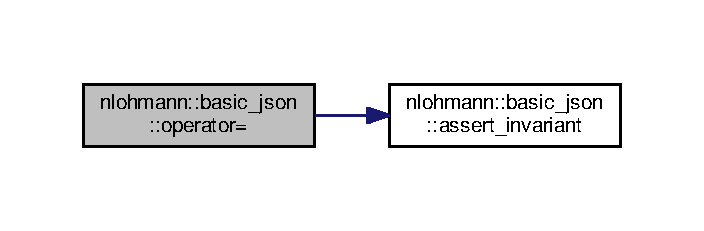
\includegraphics[width=338pt]{classnlohmann_1_1basic__json_aab256df8c5594ec693035822fa1e2904_cgraph}
\end{center}
\end{figure}
\mbox{\Hypertarget{classnlohmann_1_1basic__json_ac871e3b03fb2eeca9a8de4db2bea760f}\label{classnlohmann_1_1basic__json_ac871e3b03fb2eeca9a8de4db2bea760f}} 
\index{nlohmann\+::basic\+\_\+json@{nlohmann\+::basic\+\_\+json}!operator\mbox{[}\mbox{]}@{operator[]}}
\index{operator\mbox{[}\mbox{]}@{operator[]}!nlohmann\+::basic\+\_\+json@{nlohmann\+::basic\+\_\+json}}
\subsubsection{\texorpdfstring{operator[]()}{operator[]()}\hspace{0.1cm}{\footnotesize\ttfamily [1/10]}}
{\footnotesize\ttfamily template$<$template$<$ typename U, typename V, typename... Args $>$ class Object\+Type = std\+::map, template$<$ typename U, typename... Args $>$ class Array\+Type = std\+::vector, class String\+Type  = std\+::string, class Boolean\+Type  = bool, class Number\+Integer\+Type  = std\+::int64\+\_\+t, class Number\+Unsigned\+Type  = std\+::uint64\+\_\+t, class Number\+Float\+Type  = double, template$<$ typename U $>$ class Allocator\+Type = std\+::allocator, template$<$ typename T, typename S\+F\+I\+N\+A\+E=void $>$ class J\+S\+O\+N\+Serializer = adl\+\_\+serializer$>$ \\
\hyperlink{classnlohmann_1_1basic__json_ac6a5eddd156c776ac75ff54cfe54a5bc}{reference} \hyperlink{classnlohmann_1_1basic__json}{nlohmann\+::basic\+\_\+json}$<$ Object\+Type, Array\+Type, String\+Type, Boolean\+Type, Number\+Integer\+Type, Number\+Unsigned\+Type, Number\+Float\+Type, Allocator\+Type, J\+S\+O\+N\+Serializer $>$\+::operator\mbox{[}$\,$\mbox{]} (\begin{DoxyParamCaption}\item[{\hyperlink{classnlohmann_1_1basic__json_a39f2cd0b58106097e0e67bf185cc519b}{size\+\_\+type}}]{idx }\end{DoxyParamCaption})\hspace{0.3cm}{\ttfamily [inline]}}



access specified array element 

Returns a reference to the element at specified location {\itshape idx}.

\begin{DoxyNote}{Note}
If {\itshape idx} is beyond the range of the array (i.\+e., {\ttfamily idx $>$= \hyperlink{classnlohmann_1_1basic__json_a25e27ad0c6d53c01871c5485e1f75b96}{size()}}), then the array is silently filled up with {\ttfamily null} values to make {\ttfamily idx} a valid reference to the last stored element.
\end{DoxyNote}

\begin{DoxyParams}[1]{Parameters}
\mbox{\tt in}  & {\em idx} & index of the element to access\\
\hline
\end{DoxyParams}
\begin{DoxyReturn}{Returns}
reference to the element at index {\itshape idx} 
\end{DoxyReturn}

\begin{DoxyExceptions}{Exceptions}
{\em std\+::domain\+\_\+error} & if J\+S\+ON is not an array or null; example\+: {\ttfamily \char`\"{}cannot use operator\mbox{[}$\,$\mbox{]} with string\char`\"{}}\\
\hline
\end{DoxyExceptions}
Constant if {\itshape idx} is in the range of the array. Otherwise linear in {\ttfamily idx -\/ \hyperlink{classnlohmann_1_1basic__json_a25e27ad0c6d53c01871c5485e1f75b96}{size()}}.

\{The example below shows how array elements can be read and written using {\ttfamily \mbox{[}\mbox{]}} operator. Note the addition of {\ttfamily null} values.,operatorarray\+\_\+\+\_\+size\+\_\+type\}

\begin{DoxySince}{Since}
version 1.\+0.\+0 
\end{DoxySince}
\mbox{\Hypertarget{classnlohmann_1_1basic__json_a9cb592cd85c14f3e845e30d51cf17efb}\label{classnlohmann_1_1basic__json_a9cb592cd85c14f3e845e30d51cf17efb}} 
\index{nlohmann\+::basic\+\_\+json@{nlohmann\+::basic\+\_\+json}!operator\mbox{[}\mbox{]}@{operator[]}}
\index{operator\mbox{[}\mbox{]}@{operator[]}!nlohmann\+::basic\+\_\+json@{nlohmann\+::basic\+\_\+json}}
\subsubsection{\texorpdfstring{operator[]()}{operator[]()}\hspace{0.1cm}{\footnotesize\ttfamily [2/10]}}
{\footnotesize\ttfamily template$<$template$<$ typename U, typename V, typename... Args $>$ class Object\+Type = std\+::map, template$<$ typename U, typename... Args $>$ class Array\+Type = std\+::vector, class String\+Type  = std\+::string, class Boolean\+Type  = bool, class Number\+Integer\+Type  = std\+::int64\+\_\+t, class Number\+Unsigned\+Type  = std\+::uint64\+\_\+t, class Number\+Float\+Type  = double, template$<$ typename U $>$ class Allocator\+Type = std\+::allocator, template$<$ typename T, typename S\+F\+I\+N\+A\+E=void $>$ class J\+S\+O\+N\+Serializer = adl\+\_\+serializer$>$ \\
\hyperlink{classnlohmann_1_1basic__json_a4057c5425f4faacfe39a8046871786ca}{const\+\_\+reference} \hyperlink{classnlohmann_1_1basic__json}{nlohmann\+::basic\+\_\+json}$<$ Object\+Type, Array\+Type, String\+Type, Boolean\+Type, Number\+Integer\+Type, Number\+Unsigned\+Type, Number\+Float\+Type, Allocator\+Type, J\+S\+O\+N\+Serializer $>$\+::operator\mbox{[}$\,$\mbox{]} (\begin{DoxyParamCaption}\item[{\hyperlink{classnlohmann_1_1basic__json_a39f2cd0b58106097e0e67bf185cc519b}{size\+\_\+type}}]{idx }\end{DoxyParamCaption}) const\hspace{0.3cm}{\ttfamily [inline]}}



access specified array element 

Returns a const reference to the element at specified location {\itshape idx}.


\begin{DoxyParams}[1]{Parameters}
\mbox{\tt in}  & {\em idx} & index of the element to access\\
\hline
\end{DoxyParams}
\begin{DoxyReturn}{Returns}
const reference to the element at index {\itshape idx} 
\end{DoxyReturn}

\begin{DoxyExceptions}{Exceptions}
{\em std\+::domain\+\_\+error} & if J\+S\+ON is not an array; example\+: {\ttfamily \char`\"{}cannot use
operator\mbox{[}$\,$\mbox{]} with null\char`\"{}}\\
\hline
\end{DoxyExceptions}
Constant.

\{The example below shows how array elements can be read using the {\ttfamily \mbox{[}\mbox{]}} operator.,operatorarray\+\_\+\+\_\+size\+\_\+type\+\_\+const\}

\begin{DoxySince}{Since}
version 1.\+0.\+0 
\end{DoxySince}
Here is the call graph for this function\+:\nopagebreak
\begin{figure}[H]
\begin{center}
\leavevmode
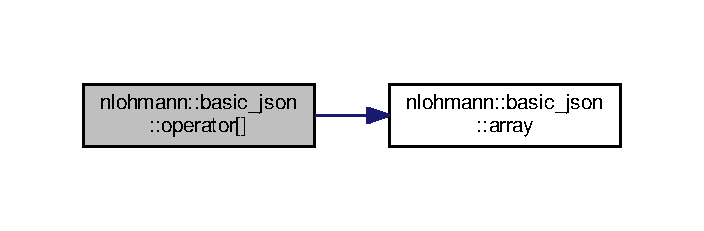
\includegraphics[width=338pt]{classnlohmann_1_1basic__json_a9cb592cd85c14f3e845e30d51cf17efb_cgraph}
\end{center}
\end{figure}
\mbox{\Hypertarget{classnlohmann_1_1basic__json_a233b02b0839ef798942dd46157cc0fe6}\label{classnlohmann_1_1basic__json_a233b02b0839ef798942dd46157cc0fe6}} 
\index{nlohmann\+::basic\+\_\+json@{nlohmann\+::basic\+\_\+json}!operator\mbox{[}\mbox{]}@{operator[]}}
\index{operator\mbox{[}\mbox{]}@{operator[]}!nlohmann\+::basic\+\_\+json@{nlohmann\+::basic\+\_\+json}}
\subsubsection{\texorpdfstring{operator[]()}{operator[]()}\hspace{0.1cm}{\footnotesize\ttfamily [3/10]}}
{\footnotesize\ttfamily template$<$template$<$ typename U, typename V, typename... Args $>$ class Object\+Type = std\+::map, template$<$ typename U, typename... Args $>$ class Array\+Type = std\+::vector, class String\+Type  = std\+::string, class Boolean\+Type  = bool, class Number\+Integer\+Type  = std\+::int64\+\_\+t, class Number\+Unsigned\+Type  = std\+::uint64\+\_\+t, class Number\+Float\+Type  = double, template$<$ typename U $>$ class Allocator\+Type = std\+::allocator, template$<$ typename T, typename S\+F\+I\+N\+A\+E=void $>$ class J\+S\+O\+N\+Serializer = adl\+\_\+serializer$>$ \\
\hyperlink{classnlohmann_1_1basic__json_ac6a5eddd156c776ac75ff54cfe54a5bc}{reference} \hyperlink{classnlohmann_1_1basic__json}{nlohmann\+::basic\+\_\+json}$<$ Object\+Type, Array\+Type, String\+Type, Boolean\+Type, Number\+Integer\+Type, Number\+Unsigned\+Type, Number\+Float\+Type, Allocator\+Type, J\+S\+O\+N\+Serializer $>$\+::operator\mbox{[}$\,$\mbox{]} (\begin{DoxyParamCaption}\item[{const typename object\+\_\+t\+::key\+\_\+type \&}]{key }\end{DoxyParamCaption})\hspace{0.3cm}{\ttfamily [inline]}}



access specified object element 

Returns a reference to the element at with specified key {\itshape key}.

\begin{DoxyNote}{Note}
If {\itshape key} is not found in the object, then it is silently added to the object and filled with a {\ttfamily null} value to make {\ttfamily key} a valid reference. In case the value was {\ttfamily null} before, it is converted to an object.
\end{DoxyNote}

\begin{DoxyParams}[1]{Parameters}
\mbox{\tt in}  & {\em key} & key of the element to access\\
\hline
\end{DoxyParams}
\begin{DoxyReturn}{Returns}
reference to the element at key {\itshape key} 
\end{DoxyReturn}

\begin{DoxyExceptions}{Exceptions}
{\em std\+::domain\+\_\+error} & if J\+S\+ON is not an object or null; example\+: {\ttfamily \char`\"{}cannot use operator\mbox{[}$\,$\mbox{]} with string\char`\"{}}\\
\hline
\end{DoxyExceptions}
Logarithmic in the size of the container.

\{The example below shows how object elements can be read and written using the {\ttfamily \mbox{[}\mbox{]}} operator.,operatorarray\+\_\+\+\_\+key\+\_\+type\}

\begin{DoxySeeAlso}{See also}
\hyperlink{classnlohmann_1_1basic__json_a93403e803947b86f4da2d1fb3345cf2c}{at(const typename object\+\_\+t\+::key\+\_\+type\&)} for access by \hyperlink{classnlohmann_1_1basic__json_ac6a5eddd156c776ac75ff54cfe54a5bc}{reference} with range checking 

\hyperlink{classnlohmann_1_1basic__json_af9c51328fbe1da75eca750be3009917a}{value()} for access by \hyperlink{classnlohmann_1_1basic__json_af9c51328fbe1da75eca750be3009917a}{value} with a default \hyperlink{classnlohmann_1_1basic__json_af9c51328fbe1da75eca750be3009917a}{value}
\end{DoxySeeAlso}
\begin{DoxySince}{Since}
version 1.\+0.\+0 
\end{DoxySince}
\mbox{\Hypertarget{classnlohmann_1_1basic__json_ab2318780e5ae692039e816b6ac32c91e}\label{classnlohmann_1_1basic__json_ab2318780e5ae692039e816b6ac32c91e}} 
\index{nlohmann\+::basic\+\_\+json@{nlohmann\+::basic\+\_\+json}!operator\mbox{[}\mbox{]}@{operator[]}}
\index{operator\mbox{[}\mbox{]}@{operator[]}!nlohmann\+::basic\+\_\+json@{nlohmann\+::basic\+\_\+json}}
\subsubsection{\texorpdfstring{operator[]()}{operator[]()}\hspace{0.1cm}{\footnotesize\ttfamily [4/10]}}
{\footnotesize\ttfamily template$<$template$<$ typename U, typename V, typename... Args $>$ class Object\+Type = std\+::map, template$<$ typename U, typename... Args $>$ class Array\+Type = std\+::vector, class String\+Type  = std\+::string, class Boolean\+Type  = bool, class Number\+Integer\+Type  = std\+::int64\+\_\+t, class Number\+Unsigned\+Type  = std\+::uint64\+\_\+t, class Number\+Float\+Type  = double, template$<$ typename U $>$ class Allocator\+Type = std\+::allocator, template$<$ typename T, typename S\+F\+I\+N\+A\+E=void $>$ class J\+S\+O\+N\+Serializer = adl\+\_\+serializer$>$ \\
\hyperlink{classnlohmann_1_1basic__json_a4057c5425f4faacfe39a8046871786ca}{const\+\_\+reference} \hyperlink{classnlohmann_1_1basic__json}{nlohmann\+::basic\+\_\+json}$<$ Object\+Type, Array\+Type, String\+Type, Boolean\+Type, Number\+Integer\+Type, Number\+Unsigned\+Type, Number\+Float\+Type, Allocator\+Type, J\+S\+O\+N\+Serializer $>$\+::operator\mbox{[}$\,$\mbox{]} (\begin{DoxyParamCaption}\item[{const typename object\+\_\+t\+::key\+\_\+type \&}]{key }\end{DoxyParamCaption}) const\hspace{0.3cm}{\ttfamily [inline]}}



read-\/only access specified object element 

Returns a const reference to the element at with specified key {\itshape key}. No bounds checking is performed.

\begin{DoxyWarning}{Warning}
If the element with key {\itshape key} does not exist, the behavior is undefined.
\end{DoxyWarning}

\begin{DoxyParams}[1]{Parameters}
\mbox{\tt in}  & {\em key} & key of the element to access\\
\hline
\end{DoxyParams}
\begin{DoxyReturn}{Returns}
const reference to the element at key {\itshape key} 
\end{DoxyReturn}
\begin{DoxyPrecond}{Precondition}
The element with key {\itshape key} must exist. {\bfseries This precondition is enforced with an assertion.}
\end{DoxyPrecond}

\begin{DoxyExceptions}{Exceptions}
{\em std\+::domain\+\_\+error} & if J\+S\+ON is not an object; example\+: {\ttfamily \char`\"{}cannot use
operator\mbox{[}$\,$\mbox{]} with null\char`\"{}}\\
\hline
\end{DoxyExceptions}
Logarithmic in the size of the container.

\{The example below shows how object elements can be read using the {\ttfamily \mbox{[}\mbox{]}} operator.,operatorarray\+\_\+\+\_\+key\+\_\+type\+\_\+const\}

\begin{DoxySeeAlso}{See also}
\hyperlink{classnlohmann_1_1basic__json_a93403e803947b86f4da2d1fb3345cf2c}{at(const typename object\+\_\+t\+::key\+\_\+type\&)} for access by \hyperlink{classnlohmann_1_1basic__json_ac6a5eddd156c776ac75ff54cfe54a5bc}{reference} with range checking 

\hyperlink{classnlohmann_1_1basic__json_af9c51328fbe1da75eca750be3009917a}{value()} for access by \hyperlink{classnlohmann_1_1basic__json_af9c51328fbe1da75eca750be3009917a}{value} with a default \hyperlink{classnlohmann_1_1basic__json_af9c51328fbe1da75eca750be3009917a}{value}
\end{DoxySeeAlso}
\begin{DoxySince}{Since}
version 1.\+0.\+0 
\end{DoxySince}
Here is the call graph for this function\+:\nopagebreak
\begin{figure}[H]
\begin{center}
\leavevmode
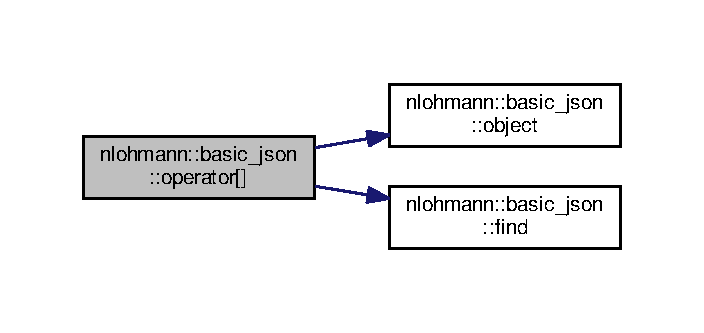
\includegraphics[width=338pt]{classnlohmann_1_1basic__json_ab2318780e5ae692039e816b6ac32c91e_cgraph}
\end{center}
\end{figure}
\mbox{\Hypertarget{classnlohmann_1_1basic__json_a1416bbec9d9a8eeca21c213cf5290868}\label{classnlohmann_1_1basic__json_a1416bbec9d9a8eeca21c213cf5290868}} 
\index{nlohmann\+::basic\+\_\+json@{nlohmann\+::basic\+\_\+json}!operator\mbox{[}\mbox{]}@{operator[]}}
\index{operator\mbox{[}\mbox{]}@{operator[]}!nlohmann\+::basic\+\_\+json@{nlohmann\+::basic\+\_\+json}}
\subsubsection{\texorpdfstring{operator[]()}{operator[]()}\hspace{0.1cm}{\footnotesize\ttfamily [5/10]}}
{\footnotesize\ttfamily template$<$template$<$ typename U, typename V, typename... Args $>$ class Object\+Type = std\+::map, template$<$ typename U, typename... Args $>$ class Array\+Type = std\+::vector, class String\+Type  = std\+::string, class Boolean\+Type  = bool, class Number\+Integer\+Type  = std\+::int64\+\_\+t, class Number\+Unsigned\+Type  = std\+::uint64\+\_\+t, class Number\+Float\+Type  = double, template$<$ typename U $>$ class Allocator\+Type = std\+::allocator, template$<$ typename T, typename S\+F\+I\+N\+A\+E=void $>$ class J\+S\+O\+N\+Serializer = adl\+\_\+serializer$>$ \\
template$<$typename T , std\+::size\+\_\+t n$>$ \\
\hyperlink{classnlohmann_1_1basic__json_ac6a5eddd156c776ac75ff54cfe54a5bc}{reference} \hyperlink{classnlohmann_1_1basic__json}{nlohmann\+::basic\+\_\+json}$<$ Object\+Type, Array\+Type, String\+Type, Boolean\+Type, Number\+Integer\+Type, Number\+Unsigned\+Type, Number\+Float\+Type, Allocator\+Type, J\+S\+O\+N\+Serializer $>$\+::operator\mbox{[}$\,$\mbox{]} (\begin{DoxyParamCaption}\item[{T $\ast$(\&)}]{key\mbox{[}n\mbox{]} }\end{DoxyParamCaption})\hspace{0.3cm}{\ttfamily [inline]}}



access specified object element 

Returns a reference to the element at with specified key {\itshape key}.

\begin{DoxyNote}{Note}
If {\itshape key} is not found in the object, then it is silently added to the object and filled with a {\ttfamily null} value to make {\ttfamily key} a valid reference. In case the value was {\ttfamily null} before, it is converted to an object.
\end{DoxyNote}

\begin{DoxyParams}[1]{Parameters}
\mbox{\tt in}  & {\em key} & key of the element to access\\
\hline
\end{DoxyParams}
\begin{DoxyReturn}{Returns}
reference to the element at key {\itshape key} 
\end{DoxyReturn}

\begin{DoxyExceptions}{Exceptions}
{\em std\+::domain\+\_\+error} & if J\+S\+ON is not an object or null; example\+: {\ttfamily \char`\"{}cannot use operator\mbox{[}$\,$\mbox{]} with string\char`\"{}}\\
\hline
\end{DoxyExceptions}
Logarithmic in the size of the container.

\{The example below shows how object elements can be read and written using the {\ttfamily \mbox{[}\mbox{]}} operator.,operatorarray\+\_\+\+\_\+key\+\_\+type\}

\begin{DoxySeeAlso}{See also}
\hyperlink{classnlohmann_1_1basic__json_a93403e803947b86f4da2d1fb3345cf2c}{at(const typename object\+\_\+t\+::key\+\_\+type\&)} for access by \hyperlink{classnlohmann_1_1basic__json_ac6a5eddd156c776ac75ff54cfe54a5bc}{reference} with range checking 

\hyperlink{classnlohmann_1_1basic__json_af9c51328fbe1da75eca750be3009917a}{value()} for access by \hyperlink{classnlohmann_1_1basic__json_af9c51328fbe1da75eca750be3009917a}{value} with a default \hyperlink{classnlohmann_1_1basic__json_af9c51328fbe1da75eca750be3009917a}{value}
\end{DoxySeeAlso}
\begin{DoxySince}{Since}
version 1.\+0.\+0 
\end{DoxySince}
\mbox{\Hypertarget{classnlohmann_1_1basic__json_ab17b18f161ecd014074790e25449094a}\label{classnlohmann_1_1basic__json_ab17b18f161ecd014074790e25449094a}} 
\index{nlohmann\+::basic\+\_\+json@{nlohmann\+::basic\+\_\+json}!operator\mbox{[}\mbox{]}@{operator[]}}
\index{operator\mbox{[}\mbox{]}@{operator[]}!nlohmann\+::basic\+\_\+json@{nlohmann\+::basic\+\_\+json}}
\subsubsection{\texorpdfstring{operator[]()}{operator[]()}\hspace{0.1cm}{\footnotesize\ttfamily [6/10]}}
{\footnotesize\ttfamily template$<$template$<$ typename U, typename V, typename... Args $>$ class Object\+Type = std\+::map, template$<$ typename U, typename... Args $>$ class Array\+Type = std\+::vector, class String\+Type  = std\+::string, class Boolean\+Type  = bool, class Number\+Integer\+Type  = std\+::int64\+\_\+t, class Number\+Unsigned\+Type  = std\+::uint64\+\_\+t, class Number\+Float\+Type  = double, template$<$ typename U $>$ class Allocator\+Type = std\+::allocator, template$<$ typename T, typename S\+F\+I\+N\+A\+E=void $>$ class J\+S\+O\+N\+Serializer = adl\+\_\+serializer$>$ \\
template$<$typename T , std\+::size\+\_\+t n$>$ \\
\hyperlink{classnlohmann_1_1basic__json_a4057c5425f4faacfe39a8046871786ca}{const\+\_\+reference} \hyperlink{classnlohmann_1_1basic__json}{nlohmann\+::basic\+\_\+json}$<$ Object\+Type, Array\+Type, String\+Type, Boolean\+Type, Number\+Integer\+Type, Number\+Unsigned\+Type, Number\+Float\+Type, Allocator\+Type, J\+S\+O\+N\+Serializer $>$\+::operator\mbox{[}$\,$\mbox{]} (\begin{DoxyParamCaption}\item[{T $\ast$(\&)}]{key\mbox{[}n\mbox{]} }\end{DoxyParamCaption}) const\hspace{0.3cm}{\ttfamily [inline]}}



read-\/only access specified object element 

Returns a const reference to the element at with specified key {\itshape key}. No bounds checking is performed.

\begin{DoxyWarning}{Warning}
If the element with key {\itshape key} does not exist, the behavior is undefined.
\end{DoxyWarning}
\begin{DoxyNote}{Note}
This function is required for compatibility reasons with Clang.
\end{DoxyNote}

\begin{DoxyParams}[1]{Parameters}
\mbox{\tt in}  & {\em key} & key of the element to access\\
\hline
\end{DoxyParams}
\begin{DoxyReturn}{Returns}
const reference to the element at key {\itshape key} 
\end{DoxyReturn}

\begin{DoxyExceptions}{Exceptions}
{\em std\+::domain\+\_\+error} & if J\+S\+ON is not an object; example\+: {\ttfamily \char`\"{}cannot use
operator\mbox{[}$\,$\mbox{]} with null\char`\"{}}\\
\hline
\end{DoxyExceptions}
Logarithmic in the size of the container.

\{The example below shows how object elements can be read using the {\ttfamily \mbox{[}\mbox{]}} operator.,operatorarray\+\_\+\+\_\+key\+\_\+type\+\_\+const\}

\begin{DoxySeeAlso}{See also}
\hyperlink{classnlohmann_1_1basic__json_a93403e803947b86f4da2d1fb3345cf2c}{at(const typename object\+\_\+t\+::key\+\_\+type\&)} for access by \hyperlink{classnlohmann_1_1basic__json_ac6a5eddd156c776ac75ff54cfe54a5bc}{reference} with range checking 

\hyperlink{classnlohmann_1_1basic__json_af9c51328fbe1da75eca750be3009917a}{value()} for access by \hyperlink{classnlohmann_1_1basic__json_af9c51328fbe1da75eca750be3009917a}{value} with a default \hyperlink{classnlohmann_1_1basic__json_af9c51328fbe1da75eca750be3009917a}{value}
\end{DoxySeeAlso}
\begin{DoxySince}{Since}
version 1.\+0.\+0 
\end{DoxySince}
\mbox{\Hypertarget{classnlohmann_1_1basic__json_abb8eaa633584b5aff9c8fcd242f25ca8}\label{classnlohmann_1_1basic__json_abb8eaa633584b5aff9c8fcd242f25ca8}} 
\index{nlohmann\+::basic\+\_\+json@{nlohmann\+::basic\+\_\+json}!operator\mbox{[}\mbox{]}@{operator[]}}
\index{operator\mbox{[}\mbox{]}@{operator[]}!nlohmann\+::basic\+\_\+json@{nlohmann\+::basic\+\_\+json}}
\subsubsection{\texorpdfstring{operator[]()}{operator[]()}\hspace{0.1cm}{\footnotesize\ttfamily [7/10]}}
{\footnotesize\ttfamily template$<$template$<$ typename U, typename V, typename... Args $>$ class Object\+Type = std\+::map, template$<$ typename U, typename... Args $>$ class Array\+Type = std\+::vector, class String\+Type  = std\+::string, class Boolean\+Type  = bool, class Number\+Integer\+Type  = std\+::int64\+\_\+t, class Number\+Unsigned\+Type  = std\+::uint64\+\_\+t, class Number\+Float\+Type  = double, template$<$ typename U $>$ class Allocator\+Type = std\+::allocator, template$<$ typename T, typename S\+F\+I\+N\+A\+E=void $>$ class J\+S\+O\+N\+Serializer = adl\+\_\+serializer$>$ \\
template$<$typename T $>$ \\
\hyperlink{classnlohmann_1_1basic__json_ac6a5eddd156c776ac75ff54cfe54a5bc}{reference} \hyperlink{classnlohmann_1_1basic__json}{nlohmann\+::basic\+\_\+json}$<$ Object\+Type, Array\+Type, String\+Type, Boolean\+Type, Number\+Integer\+Type, Number\+Unsigned\+Type, Number\+Float\+Type, Allocator\+Type, J\+S\+O\+N\+Serializer $>$\+::operator\mbox{[}$\,$\mbox{]} (\begin{DoxyParamCaption}\item[{T $\ast$}]{key }\end{DoxyParamCaption})\hspace{0.3cm}{\ttfamily [inline]}}



access specified object element 

Returns a reference to the element at with specified key {\itshape key}.

\begin{DoxyNote}{Note}
If {\itshape key} is not found in the object, then it is silently added to the object and filled with a {\ttfamily null} value to make {\ttfamily key} a valid reference. In case the value was {\ttfamily null} before, it is converted to an object.
\end{DoxyNote}

\begin{DoxyParams}[1]{Parameters}
\mbox{\tt in}  & {\em key} & key of the element to access\\
\hline
\end{DoxyParams}
\begin{DoxyReturn}{Returns}
reference to the element at key {\itshape key} 
\end{DoxyReturn}

\begin{DoxyExceptions}{Exceptions}
{\em std\+::domain\+\_\+error} & if J\+S\+ON is not an object or null; example\+: {\ttfamily \char`\"{}cannot use operator\mbox{[}$\,$\mbox{]} with string\char`\"{}}\\
\hline
\end{DoxyExceptions}
Logarithmic in the size of the container.

\{The example below shows how object elements can be read and written using the {\ttfamily \mbox{[}\mbox{]}} operator.,operatorarray\+\_\+\+\_\+key\+\_\+type\}

\begin{DoxySeeAlso}{See also}
\hyperlink{classnlohmann_1_1basic__json_a93403e803947b86f4da2d1fb3345cf2c}{at(const typename object\+\_\+t\+::key\+\_\+type\&)} for access by \hyperlink{classnlohmann_1_1basic__json_ac6a5eddd156c776ac75ff54cfe54a5bc}{reference} with range checking 

\hyperlink{classnlohmann_1_1basic__json_af9c51328fbe1da75eca750be3009917a}{value()} for access by \hyperlink{classnlohmann_1_1basic__json_af9c51328fbe1da75eca750be3009917a}{value} with a default \hyperlink{classnlohmann_1_1basic__json_af9c51328fbe1da75eca750be3009917a}{value}
\end{DoxySeeAlso}
\begin{DoxySince}{Since}
version 1.\+1.\+0 
\end{DoxySince}
\mbox{\Hypertarget{classnlohmann_1_1basic__json_a26554213cbb1722accc460ce348c860a}\label{classnlohmann_1_1basic__json_a26554213cbb1722accc460ce348c860a}} 
\index{nlohmann\+::basic\+\_\+json@{nlohmann\+::basic\+\_\+json}!operator\mbox{[}\mbox{]}@{operator[]}}
\index{operator\mbox{[}\mbox{]}@{operator[]}!nlohmann\+::basic\+\_\+json@{nlohmann\+::basic\+\_\+json}}
\subsubsection{\texorpdfstring{operator[]()}{operator[]()}\hspace{0.1cm}{\footnotesize\ttfamily [8/10]}}
{\footnotesize\ttfamily template$<$template$<$ typename U, typename V, typename... Args $>$ class Object\+Type = std\+::map, template$<$ typename U, typename... Args $>$ class Array\+Type = std\+::vector, class String\+Type  = std\+::string, class Boolean\+Type  = bool, class Number\+Integer\+Type  = std\+::int64\+\_\+t, class Number\+Unsigned\+Type  = std\+::uint64\+\_\+t, class Number\+Float\+Type  = double, template$<$ typename U $>$ class Allocator\+Type = std\+::allocator, template$<$ typename T, typename S\+F\+I\+N\+A\+E=void $>$ class J\+S\+O\+N\+Serializer = adl\+\_\+serializer$>$ \\
template$<$typename T $>$ \\
\hyperlink{classnlohmann_1_1basic__json_a4057c5425f4faacfe39a8046871786ca}{const\+\_\+reference} \hyperlink{classnlohmann_1_1basic__json}{nlohmann\+::basic\+\_\+json}$<$ Object\+Type, Array\+Type, String\+Type, Boolean\+Type, Number\+Integer\+Type, Number\+Unsigned\+Type, Number\+Float\+Type, Allocator\+Type, J\+S\+O\+N\+Serializer $>$\+::operator\mbox{[}$\,$\mbox{]} (\begin{DoxyParamCaption}\item[{T $\ast$}]{key }\end{DoxyParamCaption}) const\hspace{0.3cm}{\ttfamily [inline]}}



read-\/only access specified object element 

Returns a const reference to the element at with specified key {\itshape key}. No bounds checking is performed.

\begin{DoxyWarning}{Warning}
If the element with key {\itshape key} does not exist, the behavior is undefined.
\end{DoxyWarning}

\begin{DoxyParams}[1]{Parameters}
\mbox{\tt in}  & {\em key} & key of the element to access\\
\hline
\end{DoxyParams}
\begin{DoxyReturn}{Returns}
const reference to the element at key {\itshape key} 
\end{DoxyReturn}
\begin{DoxyPrecond}{Precondition}
The element with key {\itshape key} must exist. {\bfseries This precondition is enforced with an assertion.}
\end{DoxyPrecond}

\begin{DoxyExceptions}{Exceptions}
{\em std\+::domain\+\_\+error} & if J\+S\+ON is not an object; example\+: {\ttfamily \char`\"{}cannot use
operator\mbox{[}$\,$\mbox{]} with null\char`\"{}}\\
\hline
\end{DoxyExceptions}
Logarithmic in the size of the container.

\{The example below shows how object elements can be read using the {\ttfamily \mbox{[}\mbox{]}} operator.,operatorarray\+\_\+\+\_\+key\+\_\+type\+\_\+const\}

\begin{DoxySeeAlso}{See also}
\hyperlink{classnlohmann_1_1basic__json_a93403e803947b86f4da2d1fb3345cf2c}{at(const typename object\+\_\+t\+::key\+\_\+type\&)} for access by \hyperlink{classnlohmann_1_1basic__json_ac6a5eddd156c776ac75ff54cfe54a5bc}{reference} with range checking 

\hyperlink{classnlohmann_1_1basic__json_af9c51328fbe1da75eca750be3009917a}{value()} for access by \hyperlink{classnlohmann_1_1basic__json_af9c51328fbe1da75eca750be3009917a}{value} with a default \hyperlink{classnlohmann_1_1basic__json_af9c51328fbe1da75eca750be3009917a}{value}
\end{DoxySeeAlso}
\begin{DoxySince}{Since}
version 1.\+1.\+0 
\end{DoxySince}
Here is the call graph for this function\+:\nopagebreak
\begin{figure}[H]
\begin{center}
\leavevmode
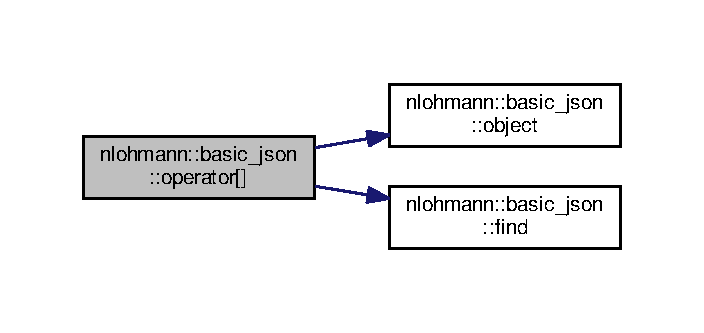
\includegraphics[width=338pt]{classnlohmann_1_1basic__json_a26554213cbb1722accc460ce348c860a_cgraph}
\end{center}
\end{figure}
\mbox{\Hypertarget{classnlohmann_1_1basic__json_ac6946dffeb3be5aa173645f0467a44b3}\label{classnlohmann_1_1basic__json_ac6946dffeb3be5aa173645f0467a44b3}} 
\index{nlohmann\+::basic\+\_\+json@{nlohmann\+::basic\+\_\+json}!operator\mbox{[}\mbox{]}@{operator[]}}
\index{operator\mbox{[}\mbox{]}@{operator[]}!nlohmann\+::basic\+\_\+json@{nlohmann\+::basic\+\_\+json}}
\subsubsection{\texorpdfstring{operator[]()}{operator[]()}\hspace{0.1cm}{\footnotesize\ttfamily [9/10]}}
{\footnotesize\ttfamily template$<$template$<$ typename U, typename V, typename... Args $>$ class Object\+Type = std\+::map, template$<$ typename U, typename... Args $>$ class Array\+Type = std\+::vector, class String\+Type  = std\+::string, class Boolean\+Type  = bool, class Number\+Integer\+Type  = std\+::int64\+\_\+t, class Number\+Unsigned\+Type  = std\+::uint64\+\_\+t, class Number\+Float\+Type  = double, template$<$ typename U $>$ class Allocator\+Type = std\+::allocator, template$<$ typename T, typename S\+F\+I\+N\+A\+E=void $>$ class J\+S\+O\+N\+Serializer = adl\+\_\+serializer$>$ \\
\hyperlink{classnlohmann_1_1basic__json_ac6a5eddd156c776ac75ff54cfe54a5bc}{reference} \hyperlink{classnlohmann_1_1basic__json}{nlohmann\+::basic\+\_\+json}$<$ Object\+Type, Array\+Type, String\+Type, Boolean\+Type, Number\+Integer\+Type, Number\+Unsigned\+Type, Number\+Float\+Type, Allocator\+Type, J\+S\+O\+N\+Serializer $>$\+::operator\mbox{[}$\,$\mbox{]} (\begin{DoxyParamCaption}\item[{const \hyperlink{classnlohmann_1_1basic__json_1_1json__pointer}{json\+\_\+pointer} \&}]{ptr }\end{DoxyParamCaption})\hspace{0.3cm}{\ttfamily [inline]}}



access specified element via J\+S\+ON Pointer 

Uses a J\+S\+ON pointer to retrieve a reference to the respective J\+S\+ON value. No bound checking is performed. Similar to \hyperlink{classnlohmann_1_1basic__json_ac871e3b03fb2eeca9a8de4db2bea760f}{operator\mbox{[}\mbox{]}}(const typename object\+\_\+t\+::key\+\_\+type\&), {\ttfamily null} values are created in arrays and objects if necessary.

In particular\+:
\begin{DoxyItemize}
\item If the J\+S\+ON pointer points to an object key that does not exist, it is created an filled with a {\ttfamily null} value before a reference to it is returned.
\item If the J\+S\+ON pointer points to an array index that does not exist, it is created an filled with a {\ttfamily null} value before a reference to it is returned. All indices between the current maximum and the given index are also filled with {\ttfamily null}.
\item The special value {\ttfamily -\/} is treated as a synonym for the index past the end.
\end{DoxyItemize}


\begin{DoxyParams}[1]{Parameters}
\mbox{\tt in}  & {\em ptr} & a J\+S\+ON pointer\\
\hline
\end{DoxyParams}
\begin{DoxyReturn}{Returns}
reference to the element pointed to by {\itshape ptr} 
\end{DoxyReturn}
Constant.


\begin{DoxyExceptions}{Exceptions}
{\em std\+::out\+\_\+of\+\_\+range} & if the J\+S\+ON pointer can not be resolved \\
\hline
{\em std\+::domain\+\_\+error} & if an array index begins with \textquotesingle{}0\textquotesingle{} \\
\hline
{\em std\+::invalid\+\_\+argument} & if an array index was not a number\\
\hline
\end{DoxyExceptions}
\{The behavior is shown in the example.,operatorjson\+\_\+pointer\}

\begin{DoxySince}{Since}
version 2.\+0.\+0 
\end{DoxySince}
Here is the call graph for this function\+:\nopagebreak
\begin{figure}[H]
\begin{center}
\leavevmode
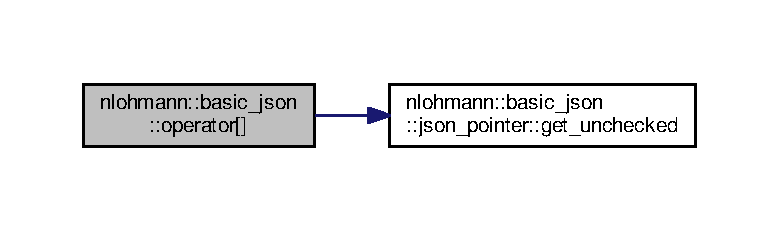
\includegraphics[width=350pt]{classnlohmann_1_1basic__json_ac6946dffeb3be5aa173645f0467a44b3_cgraph}
\end{center}
\end{figure}
\mbox{\Hypertarget{classnlohmann_1_1basic__json_a9d55e3e63b05e03a2b70cea3761f84cb}\label{classnlohmann_1_1basic__json_a9d55e3e63b05e03a2b70cea3761f84cb}} 
\index{nlohmann\+::basic\+\_\+json@{nlohmann\+::basic\+\_\+json}!operator\mbox{[}\mbox{]}@{operator[]}}
\index{operator\mbox{[}\mbox{]}@{operator[]}!nlohmann\+::basic\+\_\+json@{nlohmann\+::basic\+\_\+json}}
\subsubsection{\texorpdfstring{operator[]()}{operator[]()}\hspace{0.1cm}{\footnotesize\ttfamily [10/10]}}
{\footnotesize\ttfamily template$<$template$<$ typename U, typename V, typename... Args $>$ class Object\+Type = std\+::map, template$<$ typename U, typename... Args $>$ class Array\+Type = std\+::vector, class String\+Type  = std\+::string, class Boolean\+Type  = bool, class Number\+Integer\+Type  = std\+::int64\+\_\+t, class Number\+Unsigned\+Type  = std\+::uint64\+\_\+t, class Number\+Float\+Type  = double, template$<$ typename U $>$ class Allocator\+Type = std\+::allocator, template$<$ typename T, typename S\+F\+I\+N\+A\+E=void $>$ class J\+S\+O\+N\+Serializer = adl\+\_\+serializer$>$ \\
\hyperlink{classnlohmann_1_1basic__json_a4057c5425f4faacfe39a8046871786ca}{const\+\_\+reference} \hyperlink{classnlohmann_1_1basic__json}{nlohmann\+::basic\+\_\+json}$<$ Object\+Type, Array\+Type, String\+Type, Boolean\+Type, Number\+Integer\+Type, Number\+Unsigned\+Type, Number\+Float\+Type, Allocator\+Type, J\+S\+O\+N\+Serializer $>$\+::operator\mbox{[}$\,$\mbox{]} (\begin{DoxyParamCaption}\item[{const \hyperlink{classnlohmann_1_1basic__json_1_1json__pointer}{json\+\_\+pointer} \&}]{ptr }\end{DoxyParamCaption}) const\hspace{0.3cm}{\ttfamily [inline]}}



access specified element via J\+S\+ON Pointer 

Uses a J\+S\+ON pointer to retrieve a reference to the respective J\+S\+ON value. No bound checking is performed. The function does not change the J\+S\+ON value; no {\ttfamily null} values are created. In particular, the the special value {\ttfamily -\/} yields an exception.


\begin{DoxyParams}[1]{Parameters}
\mbox{\tt in}  & {\em ptr} & J\+S\+ON pointer to the desired element\\
\hline
\end{DoxyParams}
\begin{DoxyReturn}{Returns}
const reference to the element pointed to by {\itshape ptr} 
\end{DoxyReturn}
Constant.


\begin{DoxyExceptions}{Exceptions}
{\em std\+::out\+\_\+of\+\_\+range} & if the J\+S\+ON pointer can not be resolved \\
\hline
{\em std\+::domain\+\_\+error} & if an array index begins with \textquotesingle{}0\textquotesingle{} \\
\hline
{\em std\+::invalid\+\_\+argument} & if an array index was not a number\\
\hline
\end{DoxyExceptions}
\{The behavior is shown in the example.,operatorjson\+\_\+pointer\+\_\+const\}

\begin{DoxySince}{Since}
version 2.\+0.\+0 
\end{DoxySince}
Here is the call graph for this function\+:\nopagebreak
\begin{figure}[H]
\begin{center}
\leavevmode
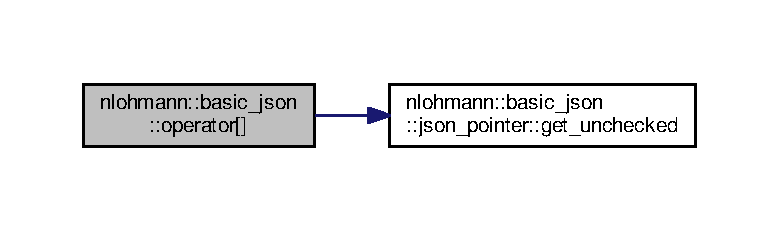
\includegraphics[width=350pt]{classnlohmann_1_1basic__json_a9d55e3e63b05e03a2b70cea3761f84cb_cgraph}
\end{center}
\end{figure}
\mbox{\Hypertarget{classnlohmann_1_1basic__json_a86f339e8449cce96b89e86635a7d389e}\label{classnlohmann_1_1basic__json_a86f339e8449cce96b89e86635a7d389e}} 
\index{nlohmann\+::basic\+\_\+json@{nlohmann\+::basic\+\_\+json}!parse@{parse}}
\index{parse@{parse}!nlohmann\+::basic\+\_\+json@{nlohmann\+::basic\+\_\+json}}
\subsubsection{\texorpdfstring{parse()}{parse()}\hspace{0.1cm}{\footnotesize\ttfamily [1/6]}}
{\footnotesize\ttfamily template$<$template$<$ typename U, typename V, typename... Args $>$ class Object\+Type = std\+::map, template$<$ typename U, typename... Args $>$ class Array\+Type = std\+::vector, class String\+Type  = std\+::string, class Boolean\+Type  = bool, class Number\+Integer\+Type  = std\+::int64\+\_\+t, class Number\+Unsigned\+Type  = std\+::uint64\+\_\+t, class Number\+Float\+Type  = double, template$<$ typename U $>$ class Allocator\+Type = std\+::allocator, template$<$ typename T, typename S\+F\+I\+N\+A\+E=void $>$ class J\+S\+O\+N\+Serializer = adl\+\_\+serializer$>$ \\
template$<$class T , std\+::size\+\_\+t N$>$ \\
static \hyperlink{classnlohmann_1_1basic__json}{basic\+\_\+json} \hyperlink{classnlohmann_1_1basic__json}{nlohmann\+::basic\+\_\+json}$<$ Object\+Type, Array\+Type, String\+Type, Boolean\+Type, Number\+Integer\+Type, Number\+Unsigned\+Type, Number\+Float\+Type, Allocator\+Type, J\+S\+O\+N\+Serializer $>$\+::parse (\begin{DoxyParamCaption}\item[{T(\&)}]{array\mbox{[}\+N\mbox{]},  }\item[{const \hyperlink{classnlohmann_1_1basic__json_aecae491e175f8767c550ae3c59e180e3}{parser\+\_\+callback\+\_\+t}}]{cb = {\ttfamily nullptr} }\end{DoxyParamCaption})\hspace{0.3cm}{\ttfamily [inline]}, {\ttfamily [static]}}



deserialize from an array 

This function reads from an array of 1-\/byte values.

\begin{DoxyPrecond}{Precondition}
Each element of the container has a size of 1 byte. Violating this precondition yields undefined behavior. {\bfseries This precondition is enforced with a static assertion.}
\end{DoxyPrecond}

\begin{DoxyParams}[1]{Parameters}
\mbox{\tt in}  & {\em array} & array to read from \\
\hline
\mbox{\tt in}  & {\em cb} & a parser callback function of type \hyperlink{classnlohmann_1_1basic__json_aecae491e175f8767c550ae3c59e180e3}{parser\+\_\+callback\+\_\+t} which is used to control the deserialization by filtering unwanted values (optional)\\
\hline
\end{DoxyParams}
\begin{DoxyReturn}{Returns}
result of the deserialization
\end{DoxyReturn}
Linear in the length of the input. The parser is a predictive L\+L(1) parser. The complexity can be higher if the parser callback function {\itshape cb} has a super-\/linear complexity.

\begin{DoxyNote}{Note}
A U\+T\+F-\/8 byte order mark is silently ignored.
\end{DoxyNote}
\{The example below demonstrates the {\ttfamily \hyperlink{classnlohmann_1_1basic__json_a86f339e8449cce96b89e86635a7d389e}{parse()}} function reading from an array.,parse\+\_\+\+\_\+array\+\_\+\+\_\+parser\+\_\+callback\+\_\+t\}

\begin{DoxySince}{Since}
version 2.\+0.\+3 
\end{DoxySince}
\mbox{\Hypertarget{classnlohmann_1_1basic__json_ab275a3e00a40189e96d244de6c8f311a}\label{classnlohmann_1_1basic__json_ab275a3e00a40189e96d244de6c8f311a}} 
\index{nlohmann\+::basic\+\_\+json@{nlohmann\+::basic\+\_\+json}!parse@{parse}}
\index{parse@{parse}!nlohmann\+::basic\+\_\+json@{nlohmann\+::basic\+\_\+json}}
\subsubsection{\texorpdfstring{parse()}{parse()}\hspace{0.1cm}{\footnotesize\ttfamily [2/6]}}
{\footnotesize\ttfamily template$<$template$<$ typename U, typename V, typename... Args $>$ class Object\+Type = std\+::map, template$<$ typename U, typename... Args $>$ class Array\+Type = std\+::vector, class String\+Type  = std\+::string, class Boolean\+Type  = bool, class Number\+Integer\+Type  = std\+::int64\+\_\+t, class Number\+Unsigned\+Type  = std\+::uint64\+\_\+t, class Number\+Float\+Type  = double, template$<$ typename U $>$ class Allocator\+Type = std\+::allocator, template$<$ typename T, typename S\+F\+I\+N\+A\+E=void $>$ class J\+S\+O\+N\+Serializer = adl\+\_\+serializer$>$ \\
template$<$typename CharT , typename std\+::enable\+\_\+if$<$ std\+::is\+\_\+pointer$<$ Char\+T $>$\+::value and std\+::is\+\_\+integral$<$ typename std\+::remove\+\_\+pointer$<$ Char\+T $>$\+::type $>$\+::value and sizeof(typename std\+::remove\+\_\+pointer$<$ Char\+T $>$\+::type)==1, int $>$\+::type  = 0$>$ \\
static \hyperlink{classnlohmann_1_1basic__json}{basic\+\_\+json} \hyperlink{classnlohmann_1_1basic__json}{nlohmann\+::basic\+\_\+json}$<$ Object\+Type, Array\+Type, String\+Type, Boolean\+Type, Number\+Integer\+Type, Number\+Unsigned\+Type, Number\+Float\+Type, Allocator\+Type, J\+S\+O\+N\+Serializer $>$\+::parse (\begin{DoxyParamCaption}\item[{const CharT}]{s,  }\item[{const \hyperlink{classnlohmann_1_1basic__json_aecae491e175f8767c550ae3c59e180e3}{parser\+\_\+callback\+\_\+t}}]{cb = {\ttfamily nullptr} }\end{DoxyParamCaption})\hspace{0.3cm}{\ttfamily [inline]}, {\ttfamily [static]}}



deserialize from string literal 


\begin{DoxyTemplParams}{Template Parameters}
{\em CharT} & character/literal type with size of 1 byte \\
\hline
\end{DoxyTemplParams}

\begin{DoxyParams}[1]{Parameters}
\mbox{\tt in}  & {\em s} & string literal to read a serialized J\+S\+ON value from \\
\hline
\mbox{\tt in}  & {\em cb} & a parser callback function of type \hyperlink{classnlohmann_1_1basic__json_aecae491e175f8767c550ae3c59e180e3}{parser\+\_\+callback\+\_\+t} which is used to control the deserialization by filtering unwanted values (optional)\\
\hline
\end{DoxyParams}
\begin{DoxyReturn}{Returns}
result of the deserialization
\end{DoxyReturn}
Linear in the length of the input. The parser is a predictive L\+L(1) parser. The complexity can be higher if the parser callback function {\itshape cb} has a super-\/linear complexity.

\begin{DoxyNote}{Note}
A U\+T\+F-\/8 byte order mark is silently ignored. 

String containers like {\ttfamily std\+::string} or \hyperlink{classnlohmann_1_1basic__json_a61f8566a1a85a424c7266fb531dca005}{string\+\_\+t} can be parsed with \hyperlink{classnlohmann_1_1basic__json_a00795fca3388571ba4a56a1ea6e0466b}{parse(const Contiguous\+Container\&, const parser\+\_\+callback\+\_\+t)}
\end{DoxyNote}
\{The example below demonstrates the {\ttfamily \hyperlink{classnlohmann_1_1basic__json_a86f339e8449cce96b89e86635a7d389e}{parse()}} function with and without callback function.,parse\+\_\+\+\_\+string\+\_\+\+\_\+parser\+\_\+callback\+\_\+t\}

\begin{DoxySeeAlso}{See also}
\hyperlink{classnlohmann_1_1basic__json_a4cd30efe5c33a7cf73a0c6495bb16054}{parse(std\+::istream\&, const parser\+\_\+callback\+\_\+t)} for a version that reads from an input stream
\end{DoxySeeAlso}
\begin{DoxySince}{Since}
version 1.\+0.\+0 (originally for \hyperlink{classnlohmann_1_1basic__json_a61f8566a1a85a424c7266fb531dca005}{string\+\_\+t}) 
\end{DoxySince}
Here is the call graph for this function\+:\nopagebreak
\begin{figure}[H]
\begin{center}
\leavevmode
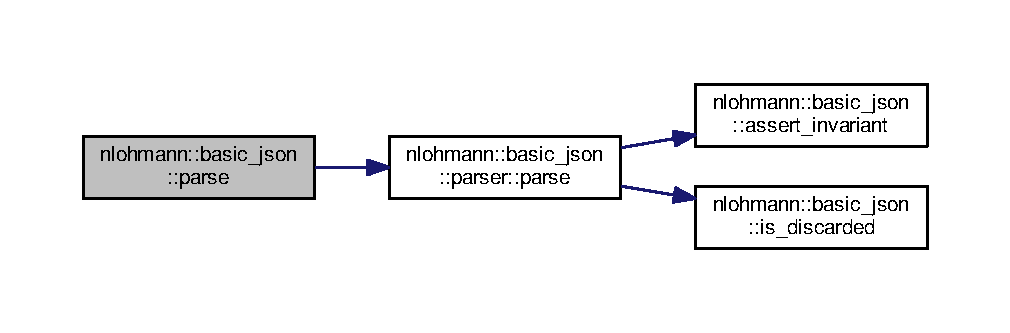
\includegraphics[width=350pt]{classnlohmann_1_1basic__json_ab275a3e00a40189e96d244de6c8f311a_cgraph}
\end{center}
\end{figure}
\mbox{\Hypertarget{classnlohmann_1_1basic__json_a4cd30efe5c33a7cf73a0c6495bb16054}\label{classnlohmann_1_1basic__json_a4cd30efe5c33a7cf73a0c6495bb16054}} 
\index{nlohmann\+::basic\+\_\+json@{nlohmann\+::basic\+\_\+json}!parse@{parse}}
\index{parse@{parse}!nlohmann\+::basic\+\_\+json@{nlohmann\+::basic\+\_\+json}}
\subsubsection{\texorpdfstring{parse()}{parse()}\hspace{0.1cm}{\footnotesize\ttfamily [3/6]}}
{\footnotesize\ttfamily template$<$template$<$ typename U, typename V, typename... Args $>$ class Object\+Type = std\+::map, template$<$ typename U, typename... Args $>$ class Array\+Type = std\+::vector, class String\+Type  = std\+::string, class Boolean\+Type  = bool, class Number\+Integer\+Type  = std\+::int64\+\_\+t, class Number\+Unsigned\+Type  = std\+::uint64\+\_\+t, class Number\+Float\+Type  = double, template$<$ typename U $>$ class Allocator\+Type = std\+::allocator, template$<$ typename T, typename S\+F\+I\+N\+A\+E=void $>$ class J\+S\+O\+N\+Serializer = adl\+\_\+serializer$>$ \\
static \hyperlink{classnlohmann_1_1basic__json}{basic\+\_\+json} \hyperlink{classnlohmann_1_1basic__json}{nlohmann\+::basic\+\_\+json}$<$ Object\+Type, Array\+Type, String\+Type, Boolean\+Type, Number\+Integer\+Type, Number\+Unsigned\+Type, Number\+Float\+Type, Allocator\+Type, J\+S\+O\+N\+Serializer $>$\+::parse (\begin{DoxyParamCaption}\item[{std\+::istream \&}]{i,  }\item[{const \hyperlink{classnlohmann_1_1basic__json_aecae491e175f8767c550ae3c59e180e3}{parser\+\_\+callback\+\_\+t}}]{cb = {\ttfamily nullptr} }\end{DoxyParamCaption})\hspace{0.3cm}{\ttfamily [inline]}, {\ttfamily [static]}}



deserialize from stream 


\begin{DoxyParams}[1]{Parameters}
\mbox{\tt in,out}  & {\em i} & stream to read a serialized J\+S\+ON value from \\
\hline
\mbox{\tt in}  & {\em cb} & a parser callback function of type \hyperlink{classnlohmann_1_1basic__json_aecae491e175f8767c550ae3c59e180e3}{parser\+\_\+callback\+\_\+t} which is used to control the deserialization by filtering unwanted values (optional)\\
\hline
\end{DoxyParams}
\begin{DoxyReturn}{Returns}
result of the deserialization
\end{DoxyReturn}
Linear in the length of the input. The parser is a predictive L\+L(1) parser. The complexity can be higher if the parser callback function {\itshape cb} has a super-\/linear complexity.

\begin{DoxyNote}{Note}
A U\+T\+F-\/8 byte order mark is silently ignored.
\end{DoxyNote}
\{The example below demonstrates the {\ttfamily \hyperlink{classnlohmann_1_1basic__json_a86f339e8449cce96b89e86635a7d389e}{parse()}} function with and without callback function.,parse\+\_\+\+\_\+istream\+\_\+\+\_\+parser\+\_\+callback\+\_\+t\}

\begin{DoxySeeAlso}{See also}
\hyperlink{classnlohmann_1_1basic__json_ab275a3e00a40189e96d244de6c8f311a}{parse(const Char\+T, const parser\+\_\+callback\+\_\+t)} for a version that reads from a string
\end{DoxySeeAlso}
\begin{DoxySince}{Since}
version 1.\+0.\+0 
\end{DoxySince}
Here is the call graph for this function\+:\nopagebreak
\begin{figure}[H]
\begin{center}
\leavevmode
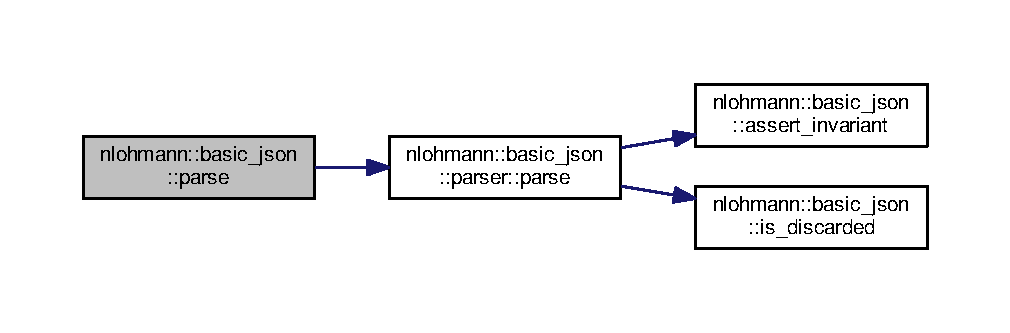
\includegraphics[width=350pt]{classnlohmann_1_1basic__json_a4cd30efe5c33a7cf73a0c6495bb16054_cgraph}
\end{center}
\end{figure}
\mbox{\Hypertarget{classnlohmann_1_1basic__json_a3bd712a1351ba28e5440fac2359da1cb}\label{classnlohmann_1_1basic__json_a3bd712a1351ba28e5440fac2359da1cb}} 
\index{nlohmann\+::basic\+\_\+json@{nlohmann\+::basic\+\_\+json}!parse@{parse}}
\index{parse@{parse}!nlohmann\+::basic\+\_\+json@{nlohmann\+::basic\+\_\+json}}
\subsubsection{\texorpdfstring{parse()}{parse()}\hspace{0.1cm}{\footnotesize\ttfamily [4/6]}}
{\footnotesize\ttfamily template$<$template$<$ typename U, typename V, typename... Args $>$ class Object\+Type = std\+::map, template$<$ typename U, typename... Args $>$ class Array\+Type = std\+::vector, class String\+Type  = std\+::string, class Boolean\+Type  = bool, class Number\+Integer\+Type  = std\+::int64\+\_\+t, class Number\+Unsigned\+Type  = std\+::uint64\+\_\+t, class Number\+Float\+Type  = double, template$<$ typename U $>$ class Allocator\+Type = std\+::allocator, template$<$ typename T, typename S\+F\+I\+N\+A\+E=void $>$ class J\+S\+O\+N\+Serializer = adl\+\_\+serializer$>$ \\
static \hyperlink{classnlohmann_1_1basic__json}{basic\+\_\+json} \hyperlink{classnlohmann_1_1basic__json}{nlohmann\+::basic\+\_\+json}$<$ Object\+Type, Array\+Type, String\+Type, Boolean\+Type, Number\+Integer\+Type, Number\+Unsigned\+Type, Number\+Float\+Type, Allocator\+Type, J\+S\+O\+N\+Serializer $>$\+::parse (\begin{DoxyParamCaption}\item[{std\+::istream \&\&}]{i,  }\item[{const \hyperlink{classnlohmann_1_1basic__json_aecae491e175f8767c550ae3c59e180e3}{parser\+\_\+callback\+\_\+t}}]{cb = {\ttfamily nullptr} }\end{DoxyParamCaption})\hspace{0.3cm}{\ttfamily [inline]}, {\ttfamily [static]}}



deserialize from stream 


\begin{DoxyParams}[1]{Parameters}
\mbox{\tt in,out}  & {\em i} & stream to read a serialized J\+S\+ON value from \\
\hline
\mbox{\tt in}  & {\em cb} & a parser callback function of type \hyperlink{classnlohmann_1_1basic__json_aecae491e175f8767c550ae3c59e180e3}{parser\+\_\+callback\+\_\+t} which is used to control the deserialization by filtering unwanted values (optional)\\
\hline
\end{DoxyParams}
\begin{DoxyReturn}{Returns}
result of the deserialization
\end{DoxyReturn}
Linear in the length of the input. The parser is a predictive L\+L(1) parser. The complexity can be higher if the parser callback function {\itshape cb} has a super-\/linear complexity.

\begin{DoxyNote}{Note}
A U\+T\+F-\/8 byte order mark is silently ignored.
\end{DoxyNote}
\{The example below demonstrates the {\ttfamily \hyperlink{classnlohmann_1_1basic__json_a86f339e8449cce96b89e86635a7d389e}{parse()}} function with and without callback function.,parse\+\_\+\+\_\+istream\+\_\+\+\_\+parser\+\_\+callback\+\_\+t\}

\begin{DoxySeeAlso}{See also}
\hyperlink{classnlohmann_1_1basic__json_ab275a3e00a40189e96d244de6c8f311a}{parse(const Char\+T, const parser\+\_\+callback\+\_\+t)} for a version that reads from a string
\end{DoxySeeAlso}
\begin{DoxySince}{Since}
version 1.\+0.\+0 
\end{DoxySince}
Here is the call graph for this function\+:\nopagebreak
\begin{figure}[H]
\begin{center}
\leavevmode
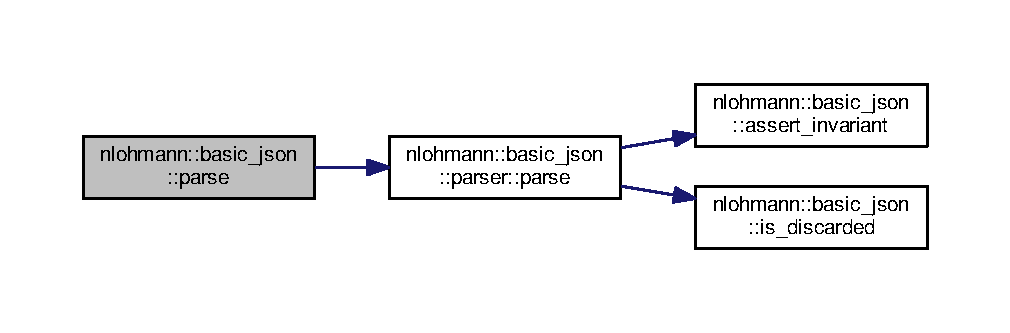
\includegraphics[width=350pt]{classnlohmann_1_1basic__json_a3bd712a1351ba28e5440fac2359da1cb_cgraph}
\end{center}
\end{figure}
\mbox{\Hypertarget{classnlohmann_1_1basic__json_a360d37260add46be89881db2366fe343}\label{classnlohmann_1_1basic__json_a360d37260add46be89881db2366fe343}} 
\index{nlohmann\+::basic\+\_\+json@{nlohmann\+::basic\+\_\+json}!parse@{parse}}
\index{parse@{parse}!nlohmann\+::basic\+\_\+json@{nlohmann\+::basic\+\_\+json}}
\subsubsection{\texorpdfstring{parse()}{parse()}\hspace{0.1cm}{\footnotesize\ttfamily [5/6]}}
{\footnotesize\ttfamily template$<$template$<$ typename U, typename V, typename... Args $>$ class Object\+Type = std\+::map, template$<$ typename U, typename... Args $>$ class Array\+Type = std\+::vector, class String\+Type  = std\+::string, class Boolean\+Type  = bool, class Number\+Integer\+Type  = std\+::int64\+\_\+t, class Number\+Unsigned\+Type  = std\+::uint64\+\_\+t, class Number\+Float\+Type  = double, template$<$ typename U $>$ class Allocator\+Type = std\+::allocator, template$<$ typename T, typename S\+F\+I\+N\+A\+E=void $>$ class J\+S\+O\+N\+Serializer = adl\+\_\+serializer$>$ \\
template$<$class Iterator\+Type , typename std\+::enable\+\_\+if$<$ std\+::is\+\_\+base\+\_\+of$<$ std\+::random\+\_\+access\+\_\+iterator\+\_\+tag, typename std\+::iterator\+\_\+traits$<$ Iterator\+Type $>$\+::iterator\+\_\+category $>$\+::value, int $>$\+::type  = 0$>$ \\
static \hyperlink{classnlohmann_1_1basic__json}{basic\+\_\+json} \hyperlink{classnlohmann_1_1basic__json}{nlohmann\+::basic\+\_\+json}$<$ Object\+Type, Array\+Type, String\+Type, Boolean\+Type, Number\+Integer\+Type, Number\+Unsigned\+Type, Number\+Float\+Type, Allocator\+Type, J\+S\+O\+N\+Serializer $>$\+::parse (\begin{DoxyParamCaption}\item[{Iterator\+Type}]{first,  }\item[{Iterator\+Type}]{last,  }\item[{const \hyperlink{classnlohmann_1_1basic__json_aecae491e175f8767c550ae3c59e180e3}{parser\+\_\+callback\+\_\+t}}]{cb = {\ttfamily nullptr} }\end{DoxyParamCaption})\hspace{0.3cm}{\ttfamily [inline]}, {\ttfamily [static]}}



deserialize from an iterator range with contiguous storage 

This function reads from an iterator range of a container with contiguous storage of 1-\/byte values. Compatible container types include {\ttfamily std\+::vector}, {\ttfamily std\+::string}, {\ttfamily std\+::array}, {\ttfamily std\+::valarray}, and {\ttfamily std\+::initializer\+\_\+list}. Furthermore, C-\/style arrays can be used with {\ttfamily std\+::begin()}/{\ttfamily std\+::end()}. User-\/defined containers can be used as long as they implement random-\/access iterators and a contiguous storage.

\begin{DoxyPrecond}{Precondition}
The iterator range is contiguous. Violating this precondition yields undefined behavior. {\bfseries This precondition is enforced with an assertion.} 

Each element in the range has a size of 1 byte. Violating this precondition yields undefined behavior. {\bfseries This precondition is enforced with a static assertion.}
\end{DoxyPrecond}
\begin{DoxyWarning}{Warning}
There is no way to enforce all preconditions at compile-\/time. If the function is called with noncompliant iterators and with assertions switched off, the behavior is undefined and will most likely yield segmentation violation.
\end{DoxyWarning}

\begin{DoxyTemplParams}{Template Parameters}
{\em Iterator\+Type} & iterator of container with contiguous storage \\
\hline
\end{DoxyTemplParams}

\begin{DoxyParams}[1]{Parameters}
\mbox{\tt in}  & {\em first} & begin of the range to parse (included) \\
\hline
\mbox{\tt in}  & {\em last} & end of the range to parse (excluded) \\
\hline
\mbox{\tt in}  & {\em cb} & a parser callback function of type \hyperlink{classnlohmann_1_1basic__json_aecae491e175f8767c550ae3c59e180e3}{parser\+\_\+callback\+\_\+t} which is used to control the deserialization by filtering unwanted values (optional)\\
\hline
\end{DoxyParams}
\begin{DoxyReturn}{Returns}
result of the deserialization
\end{DoxyReturn}
Linear in the length of the input. The parser is a predictive L\+L(1) parser. The complexity can be higher if the parser callback function {\itshape cb} has a super-\/linear complexity.

\begin{DoxyNote}{Note}
A U\+T\+F-\/8 byte order mark is silently ignored.
\end{DoxyNote}
\{The example below demonstrates the {\ttfamily \hyperlink{classnlohmann_1_1basic__json_a86f339e8449cce96b89e86635a7d389e}{parse()}} function reading from an iterator range.,parse\+\_\+\+\_\+iteratortype\+\_\+\+\_\+parser\+\_\+callback\+\_\+t\}

\begin{DoxySince}{Since}
version 2.\+0.\+3 
\end{DoxySince}
Here is the call graph for this function\+:\nopagebreak
\begin{figure}[H]
\begin{center}
\leavevmode
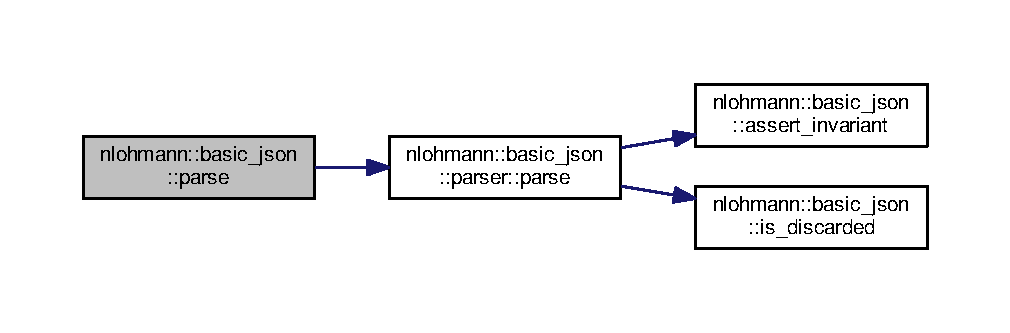
\includegraphics[width=350pt]{classnlohmann_1_1basic__json_a360d37260add46be89881db2366fe343_cgraph}
\end{center}
\end{figure}
\mbox{\Hypertarget{classnlohmann_1_1basic__json_a00795fca3388571ba4a56a1ea6e0466b}\label{classnlohmann_1_1basic__json_a00795fca3388571ba4a56a1ea6e0466b}} 
\index{nlohmann\+::basic\+\_\+json@{nlohmann\+::basic\+\_\+json}!parse@{parse}}
\index{parse@{parse}!nlohmann\+::basic\+\_\+json@{nlohmann\+::basic\+\_\+json}}
\subsubsection{\texorpdfstring{parse()}{parse()}\hspace{0.1cm}{\footnotesize\ttfamily [6/6]}}
{\footnotesize\ttfamily template$<$template$<$ typename U, typename V, typename... Args $>$ class Object\+Type = std\+::map, template$<$ typename U, typename... Args $>$ class Array\+Type = std\+::vector, class String\+Type  = std\+::string, class Boolean\+Type  = bool, class Number\+Integer\+Type  = std\+::int64\+\_\+t, class Number\+Unsigned\+Type  = std\+::uint64\+\_\+t, class Number\+Float\+Type  = double, template$<$ typename U $>$ class Allocator\+Type = std\+::allocator, template$<$ typename T, typename S\+F\+I\+N\+A\+E=void $>$ class J\+S\+O\+N\+Serializer = adl\+\_\+serializer$>$ \\
template$<$class Contiguous\+Container , typename std\+::enable\+\_\+if$<$ not std\+::is\+\_\+pointer$<$ Contiguous\+Container $>$\+::value and std\+::is\+\_\+base\+\_\+of$<$ std\+::random\+\_\+access\+\_\+iterator\+\_\+tag, typename std\+::iterator\+\_\+traits$<$ decltype(std\+::begin(std\+::declval$<$ Contiguous\+Container const $>$()))$>$\+::iterator\+\_\+category $>$\+::value, int $>$\+::type  = 0$>$ \\
static \hyperlink{classnlohmann_1_1basic__json}{basic\+\_\+json} \hyperlink{classnlohmann_1_1basic__json}{nlohmann\+::basic\+\_\+json}$<$ Object\+Type, Array\+Type, String\+Type, Boolean\+Type, Number\+Integer\+Type, Number\+Unsigned\+Type, Number\+Float\+Type, Allocator\+Type, J\+S\+O\+N\+Serializer $>$\+::parse (\begin{DoxyParamCaption}\item[{const Contiguous\+Container \&}]{c,  }\item[{const \hyperlink{classnlohmann_1_1basic__json_aecae491e175f8767c550ae3c59e180e3}{parser\+\_\+callback\+\_\+t}}]{cb = {\ttfamily nullptr} }\end{DoxyParamCaption})\hspace{0.3cm}{\ttfamily [inline]}, {\ttfamily [static]}}



deserialize from a container with contiguous storage 

This function reads from a container with contiguous storage of 1-\/byte values. Compatible container types include {\ttfamily std\+::vector}, {\ttfamily std\+::string}, {\ttfamily std\+::array}, and {\ttfamily std\+::initializer\+\_\+list}. User-\/defined containers can be used as long as they implement random-\/access iterators and a contiguous storage.

\begin{DoxyPrecond}{Precondition}
The container storage is contiguous. Violating this precondition yields undefined behavior. {\bfseries This precondition is enforced with an assertion.} 

Each element of the container has a size of 1 byte. Violating this precondition yields undefined behavior. {\bfseries This precondition is enforced with a static assertion.}
\end{DoxyPrecond}
\begin{DoxyWarning}{Warning}
There is no way to enforce all preconditions at compile-\/time. If the function is called with a noncompliant container and with assertions switched off, the behavior is undefined and will most likely yield segmentation violation.
\end{DoxyWarning}

\begin{DoxyTemplParams}{Template Parameters}
{\em Contiguous\+Container} & container type with contiguous storage \\
\hline
\end{DoxyTemplParams}

\begin{DoxyParams}[1]{Parameters}
\mbox{\tt in}  & {\em c} & container to read from \\
\hline
\mbox{\tt in}  & {\em cb} & a parser callback function of type \hyperlink{classnlohmann_1_1basic__json_aecae491e175f8767c550ae3c59e180e3}{parser\+\_\+callback\+\_\+t} which is used to control the deserialization by filtering unwanted values (optional)\\
\hline
\end{DoxyParams}
\begin{DoxyReturn}{Returns}
result of the deserialization
\end{DoxyReturn}
Linear in the length of the input. The parser is a predictive L\+L(1) parser. The complexity can be higher if the parser callback function {\itshape cb} has a super-\/linear complexity.

\begin{DoxyNote}{Note}
A U\+T\+F-\/8 byte order mark is silently ignored.
\end{DoxyNote}
\{The example below demonstrates the {\ttfamily \hyperlink{classnlohmann_1_1basic__json_a86f339e8449cce96b89e86635a7d389e}{parse()}} function reading from a contiguous container.,parse\+\_\+\+\_\+contiguouscontainer\+\_\+\+\_\+parser\+\_\+callback\+\_\+t\}

\begin{DoxySince}{Since}
version 2.\+0.\+3 
\end{DoxySince}
\mbox{\Hypertarget{classnlohmann_1_1basic__json_a81e0c41a4a9dff4df2f6973f7f8b2a83}\label{classnlohmann_1_1basic__json_a81e0c41a4a9dff4df2f6973f7f8b2a83}} 
\index{nlohmann\+::basic\+\_\+json@{nlohmann\+::basic\+\_\+json}!patch@{patch}}
\index{patch@{patch}!nlohmann\+::basic\+\_\+json@{nlohmann\+::basic\+\_\+json}}
\subsubsection{\texorpdfstring{patch()}{patch()}}
{\footnotesize\ttfamily template$<$template$<$ typename U, typename V, typename... Args $>$ class Object\+Type = std\+::map, template$<$ typename U, typename... Args $>$ class Array\+Type = std\+::vector, class String\+Type  = std\+::string, class Boolean\+Type  = bool, class Number\+Integer\+Type  = std\+::int64\+\_\+t, class Number\+Unsigned\+Type  = std\+::uint64\+\_\+t, class Number\+Float\+Type  = double, template$<$ typename U $>$ class Allocator\+Type = std\+::allocator, template$<$ typename T, typename S\+F\+I\+N\+A\+E=void $>$ class J\+S\+O\+N\+Serializer = adl\+\_\+serializer$>$ \\
\hyperlink{classnlohmann_1_1basic__json}{basic\+\_\+json} \hyperlink{classnlohmann_1_1basic__json}{nlohmann\+::basic\+\_\+json}$<$ Object\+Type, Array\+Type, String\+Type, Boolean\+Type, Number\+Integer\+Type, Number\+Unsigned\+Type, Number\+Float\+Type, Allocator\+Type, J\+S\+O\+N\+Serializer $>$\+::patch (\begin{DoxyParamCaption}\item[{const \hyperlink{classnlohmann_1_1basic__json}{basic\+\_\+json}$<$ Object\+Type, Array\+Type, String\+Type, Boolean\+Type, Number\+Integer\+Type, Number\+Unsigned\+Type, Number\+Float\+Type, Allocator\+Type, J\+S\+O\+N\+Serializer $>$ \&}]{json\+\_\+patch }\end{DoxyParamCaption}) const\hspace{0.3cm}{\ttfamily [inline]}}



applies a J\+S\+ON patch 

\href{http://jsonpatch.com}{\tt J\+S\+ON Patch} defines a J\+S\+ON document structure for expressing a sequence of operations to apply to a J\+S\+ON) document. With this function, a J\+S\+ON Patch is applied to the current J\+S\+ON value by executing all operations from the patch.


\begin{DoxyParams}[1]{Parameters}
\mbox{\tt in}  & {\em json\+\_\+patch} & J\+S\+ON patch document \\
\hline
\end{DoxyParams}
\begin{DoxyReturn}{Returns}
patched document
\end{DoxyReturn}
\begin{DoxyNote}{Note}
The application of a patch is atomic\+: Either all operations succeed and the patched document is returned or an exception is thrown. In any case, the original value is not changed\+: the patch is applied to a copy of the value.
\end{DoxyNote}

\begin{DoxyExceptions}{Exceptions}
{\em std\+::out\+\_\+of\+\_\+range} & if a J\+S\+ON pointer inside the patch could not be resolved successfully in the current J\+S\+ON value; example\+: {\ttfamily \char`\"{}key baz
not found\char`\"{}} \\
\hline
{\em invalid\+\_\+argument} & if the J\+S\+ON patch is malformed (e.\+g., mandatory attributes are missing); example\+: {\ttfamily \char`\"{}operation add must have member path\char`\"{}}\\
\hline
\end{DoxyExceptions}
Linear in the size of the J\+S\+ON value and the length of the J\+S\+ON patch. As usually only a fraction of the J\+S\+ON value is affected by the patch, the complexity can usually be neglected.

\{The following code shows how a J\+S\+ON patch is applied to a value.,patch\}

\begin{DoxySeeAlso}{See also}
\hyperlink{classnlohmann_1_1basic__json_a543bd5f7490de54c875b2c0912dc9a49}{diff} -- \hyperlink{classnlohmann_1_1basic__json_a81100399cf3e2be457937be7db3f5729}{create} a J\+S\+ON \hyperlink{classnlohmann_1_1basic__json_a81e0c41a4a9dff4df2f6973f7f8b2a83}{patch} by comparing two J\+S\+ON values

\href{https://tools.ietf.org/html/rfc6902}{\tt R\+FC 6902 (J\+S\+ON Patch)} 

\href{https://tools.ietf.org/html/rfc6901}{\tt R\+FC 6901 (J\+S\+ON Pointer)}
\end{DoxySeeAlso}
\begin{DoxySince}{Since}
version 2.\+0.\+0 
\end{DoxySince}
Here is the call graph for this function\+:\nopagebreak
\begin{figure}[H]
\begin{center}
\leavevmode
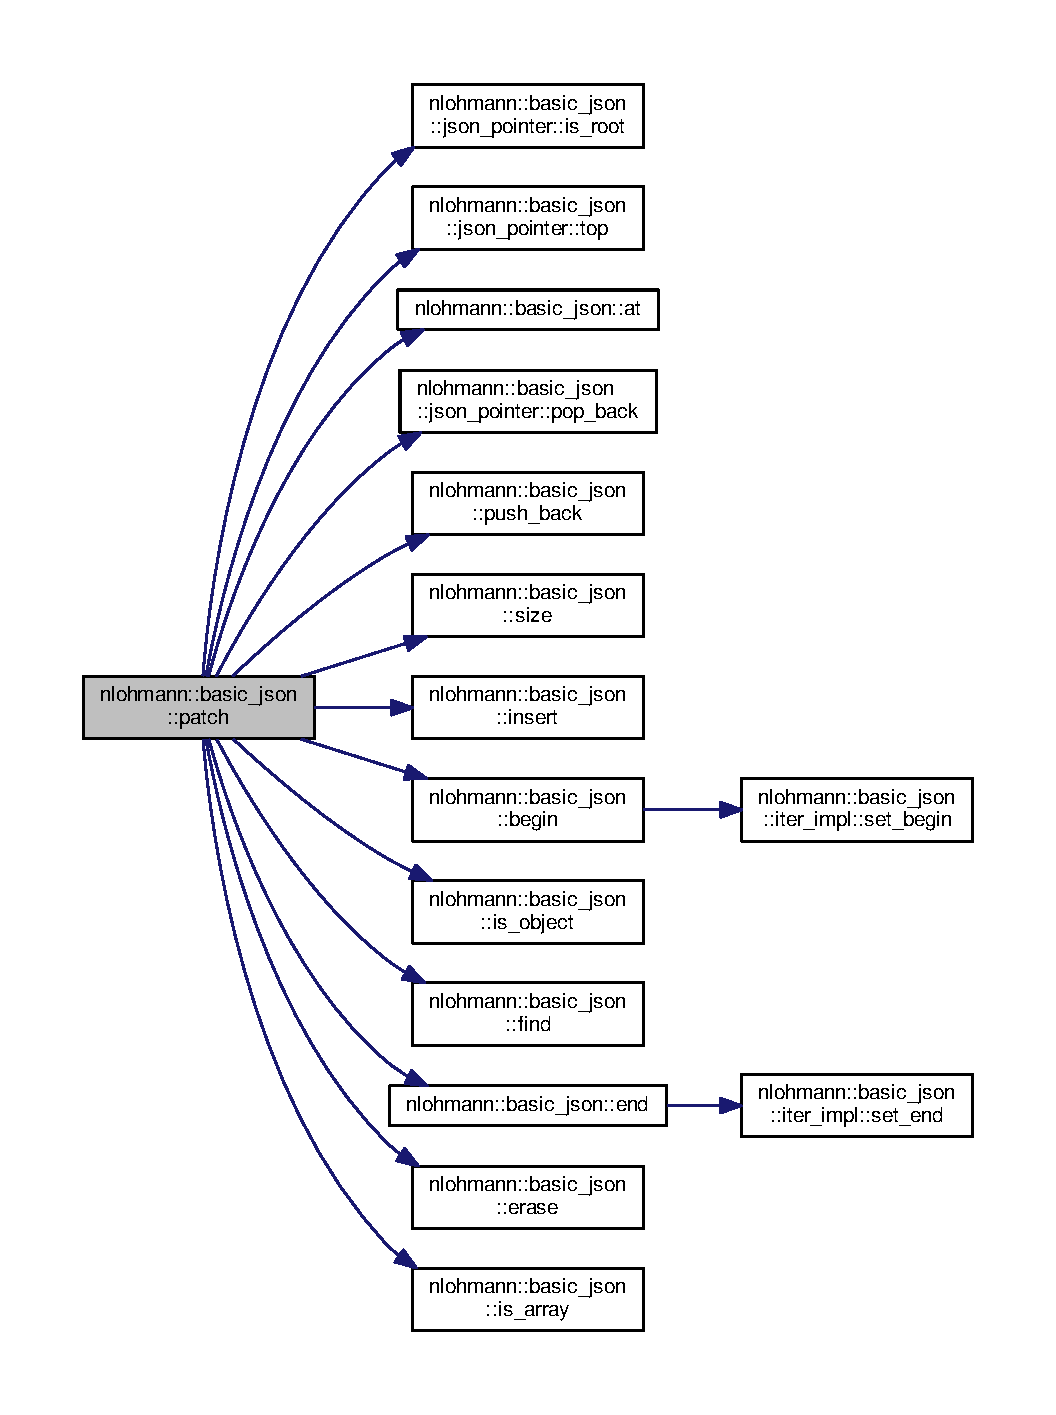
\includegraphics[width=350pt]{classnlohmann_1_1basic__json_a81e0c41a4a9dff4df2f6973f7f8b2a83_cgraph}
\end{center}
\end{figure}
\mbox{\Hypertarget{classnlohmann_1_1basic__json_ac8e523ddc8c2dd7e5d2daf0d49a9c0d7}\label{classnlohmann_1_1basic__json_ac8e523ddc8c2dd7e5d2daf0d49a9c0d7}} 
\index{nlohmann\+::basic\+\_\+json@{nlohmann\+::basic\+\_\+json}!push\+\_\+back@{push\+\_\+back}}
\index{push\+\_\+back@{push\+\_\+back}!nlohmann\+::basic\+\_\+json@{nlohmann\+::basic\+\_\+json}}
\subsubsection{\texorpdfstring{push\+\_\+back()}{push\_back()}\hspace{0.1cm}{\footnotesize\ttfamily [1/4]}}
{\footnotesize\ttfamily template$<$template$<$ typename U, typename V, typename... Args $>$ class Object\+Type = std\+::map, template$<$ typename U, typename... Args $>$ class Array\+Type = std\+::vector, class String\+Type  = std\+::string, class Boolean\+Type  = bool, class Number\+Integer\+Type  = std\+::int64\+\_\+t, class Number\+Unsigned\+Type  = std\+::uint64\+\_\+t, class Number\+Float\+Type  = double, template$<$ typename U $>$ class Allocator\+Type = std\+::allocator, template$<$ typename T, typename S\+F\+I\+N\+A\+E=void $>$ class J\+S\+O\+N\+Serializer = adl\+\_\+serializer$>$ \\
void \hyperlink{classnlohmann_1_1basic__json}{nlohmann\+::basic\+\_\+json}$<$ Object\+Type, Array\+Type, String\+Type, Boolean\+Type, Number\+Integer\+Type, Number\+Unsigned\+Type, Number\+Float\+Type, Allocator\+Type, J\+S\+O\+N\+Serializer $>$\+::push\+\_\+back (\begin{DoxyParamCaption}\item[{\hyperlink{classnlohmann_1_1basic__json}{basic\+\_\+json}$<$ Object\+Type, Array\+Type, String\+Type, Boolean\+Type, Number\+Integer\+Type, Number\+Unsigned\+Type, Number\+Float\+Type, Allocator\+Type, J\+S\+O\+N\+Serializer $>$ \&\&}]{val }\end{DoxyParamCaption})\hspace{0.3cm}{\ttfamily [inline]}}



add an object to an array 

Appends the given element {\itshape val} to the end of the J\+S\+ON value. If the function is called on a J\+S\+ON null value, an empty array is created before appending {\itshape val}.


\begin{DoxyParams}[1]{Parameters}
\mbox{\tt in}  & {\em val} & the value to add to the J\+S\+ON array\\
\hline
\end{DoxyParams}

\begin{DoxyExceptions}{Exceptions}
{\em std\+::domain\+\_\+error} & when called on a type other than J\+S\+ON array or null; example\+: {\ttfamily \char`\"{}cannot use push\+\_\+back() with number\char`\"{}}\\
\hline
\end{DoxyExceptions}
Amortized constant.

\{The example shows how {\ttfamily \hyperlink{classnlohmann_1_1basic__json_ac8e523ddc8c2dd7e5d2daf0d49a9c0d7}{push\+\_\+back()}} and {\ttfamily +=} can be used to add elements to a J\+S\+ON array. Note how the {\ttfamily null} value was silently converted to a J\+S\+ON array.,push\+\_\+back\}

\begin{DoxySince}{Since}
version 1.\+0.\+0 
\end{DoxySince}
\mbox{\Hypertarget{classnlohmann_1_1basic__json_ab4384af330b79de0e5f279576803a2c7}\label{classnlohmann_1_1basic__json_ab4384af330b79de0e5f279576803a2c7}} 
\index{nlohmann\+::basic\+\_\+json@{nlohmann\+::basic\+\_\+json}!push\+\_\+back@{push\+\_\+back}}
\index{push\+\_\+back@{push\+\_\+back}!nlohmann\+::basic\+\_\+json@{nlohmann\+::basic\+\_\+json}}
\subsubsection{\texorpdfstring{push\+\_\+back()}{push\_back()}\hspace{0.1cm}{\footnotesize\ttfamily [2/4]}}
{\footnotesize\ttfamily template$<$template$<$ typename U, typename V, typename... Args $>$ class Object\+Type = std\+::map, template$<$ typename U, typename... Args $>$ class Array\+Type = std\+::vector, class String\+Type  = std\+::string, class Boolean\+Type  = bool, class Number\+Integer\+Type  = std\+::int64\+\_\+t, class Number\+Unsigned\+Type  = std\+::uint64\+\_\+t, class Number\+Float\+Type  = double, template$<$ typename U $>$ class Allocator\+Type = std\+::allocator, template$<$ typename T, typename S\+F\+I\+N\+A\+E=void $>$ class J\+S\+O\+N\+Serializer = adl\+\_\+serializer$>$ \\
void \hyperlink{classnlohmann_1_1basic__json}{nlohmann\+::basic\+\_\+json}$<$ Object\+Type, Array\+Type, String\+Type, Boolean\+Type, Number\+Integer\+Type, Number\+Unsigned\+Type, Number\+Float\+Type, Allocator\+Type, J\+S\+O\+N\+Serializer $>$\+::push\+\_\+back (\begin{DoxyParamCaption}\item[{const \hyperlink{classnlohmann_1_1basic__json}{basic\+\_\+json}$<$ Object\+Type, Array\+Type, String\+Type, Boolean\+Type, Number\+Integer\+Type, Number\+Unsigned\+Type, Number\+Float\+Type, Allocator\+Type, J\+S\+O\+N\+Serializer $>$ \&}]{val }\end{DoxyParamCaption})\hspace{0.3cm}{\ttfamily [inline]}}



add an object to an array 

add an object to an array Appends the given element {\itshape val} to the end of the J\+S\+ON value. If the function is called on a J\+S\+ON null value, an empty array is created before appending {\itshape val}.


\begin{DoxyParams}[1]{Parameters}
\mbox{\tt in}  & {\em val} & the value to add to the J\+S\+ON array\\
\hline
\end{DoxyParams}

\begin{DoxyExceptions}{Exceptions}
{\em std\+::domain\+\_\+error} & when called on a type other than J\+S\+ON array or null; example\+: {\ttfamily \char`\"{}cannot use push\+\_\+back() with number\char`\"{}}\\
\hline
\end{DoxyExceptions}
Amortized constant.

\{The example shows how {\ttfamily \hyperlink{classnlohmann_1_1basic__json_ac8e523ddc8c2dd7e5d2daf0d49a9c0d7}{push\+\_\+back()}} and {\ttfamily +=} can be used to add elements to a J\+S\+ON array. Note how the {\ttfamily null} value was silently converted to a J\+S\+ON array.,push\+\_\+back\}

\begin{DoxySince}{Since}
version 1.\+0.\+0 
\end{DoxySince}
\mbox{\Hypertarget{classnlohmann_1_1basic__json_ae11a3a51782c058fff2f6550cdfb9b3c}\label{classnlohmann_1_1basic__json_ae11a3a51782c058fff2f6550cdfb9b3c}} 
\index{nlohmann\+::basic\+\_\+json@{nlohmann\+::basic\+\_\+json}!push\+\_\+back@{push\+\_\+back}}
\index{push\+\_\+back@{push\+\_\+back}!nlohmann\+::basic\+\_\+json@{nlohmann\+::basic\+\_\+json}}
\subsubsection{\texorpdfstring{push\+\_\+back()}{push\_back()}\hspace{0.1cm}{\footnotesize\ttfamily [3/4]}}
{\footnotesize\ttfamily template$<$template$<$ typename U, typename V, typename... Args $>$ class Object\+Type = std\+::map, template$<$ typename U, typename... Args $>$ class Array\+Type = std\+::vector, class String\+Type  = std\+::string, class Boolean\+Type  = bool, class Number\+Integer\+Type  = std\+::int64\+\_\+t, class Number\+Unsigned\+Type  = std\+::uint64\+\_\+t, class Number\+Float\+Type  = double, template$<$ typename U $>$ class Allocator\+Type = std\+::allocator, template$<$ typename T, typename S\+F\+I\+N\+A\+E=void $>$ class J\+S\+O\+N\+Serializer = adl\+\_\+serializer$>$ \\
void \hyperlink{classnlohmann_1_1basic__json}{nlohmann\+::basic\+\_\+json}$<$ Object\+Type, Array\+Type, String\+Type, Boolean\+Type, Number\+Integer\+Type, Number\+Unsigned\+Type, Number\+Float\+Type, Allocator\+Type, J\+S\+O\+N\+Serializer $>$\+::push\+\_\+back (\begin{DoxyParamCaption}\item[{const typename object\+\_\+t\+::value\+\_\+type \&}]{val }\end{DoxyParamCaption})\hspace{0.3cm}{\ttfamily [inline]}}



add an object to an object 

Inserts the given element {\itshape val} to the J\+S\+ON object. If the function is called on a J\+S\+ON null value, an empty object is created before inserting {\itshape val}.


\begin{DoxyParams}[1]{Parameters}
\mbox{\tt in}  & {\em val} & the value to add to the J\+S\+ON object\\
\hline
\end{DoxyParams}

\begin{DoxyExceptions}{Exceptions}
{\em std\+::domain\+\_\+error} & when called on a type other than J\+S\+ON object or null; example\+: {\ttfamily \char`\"{}cannot use push\+\_\+back() with number\char`\"{}}\\
\hline
\end{DoxyExceptions}
Logarithmic in the size of the container, O(log({\ttfamily \hyperlink{classnlohmann_1_1basic__json_a25e27ad0c6d53c01871c5485e1f75b96}{size()}})).

\{The example shows how {\ttfamily \hyperlink{classnlohmann_1_1basic__json_ac8e523ddc8c2dd7e5d2daf0d49a9c0d7}{push\+\_\+back()}} and {\ttfamily +=} can be used to add elements to a J\+S\+ON object. Note how the {\ttfamily null} value was silently converted to a J\+S\+ON object.,push\+\_\+back\+\_\+\+\_\+object\+\_\+t\+\_\+\+\_\+value\}

\begin{DoxySince}{Since}
version 1.\+0.\+0 
\end{DoxySince}
\mbox{\Hypertarget{classnlohmann_1_1basic__json_ab2716cbe2e997ab8309926b87f044434}\label{classnlohmann_1_1basic__json_ab2716cbe2e997ab8309926b87f044434}} 
\index{nlohmann\+::basic\+\_\+json@{nlohmann\+::basic\+\_\+json}!push\+\_\+back@{push\+\_\+back}}
\index{push\+\_\+back@{push\+\_\+back}!nlohmann\+::basic\+\_\+json@{nlohmann\+::basic\+\_\+json}}
\subsubsection{\texorpdfstring{push\+\_\+back()}{push\_back()}\hspace{0.1cm}{\footnotesize\ttfamily [4/4]}}
{\footnotesize\ttfamily template$<$template$<$ typename U, typename V, typename... Args $>$ class Object\+Type = std\+::map, template$<$ typename U, typename... Args $>$ class Array\+Type = std\+::vector, class String\+Type  = std\+::string, class Boolean\+Type  = bool, class Number\+Integer\+Type  = std\+::int64\+\_\+t, class Number\+Unsigned\+Type  = std\+::uint64\+\_\+t, class Number\+Float\+Type  = double, template$<$ typename U $>$ class Allocator\+Type = std\+::allocator, template$<$ typename T, typename S\+F\+I\+N\+A\+E=void $>$ class J\+S\+O\+N\+Serializer = adl\+\_\+serializer$>$ \\
void \hyperlink{classnlohmann_1_1basic__json}{nlohmann\+::basic\+\_\+json}$<$ Object\+Type, Array\+Type, String\+Type, Boolean\+Type, Number\+Integer\+Type, Number\+Unsigned\+Type, Number\+Float\+Type, Allocator\+Type, J\+S\+O\+N\+Serializer $>$\+::push\+\_\+back (\begin{DoxyParamCaption}\item[{std\+::initializer\+\_\+list$<$ \hyperlink{classnlohmann_1_1basic__json}{basic\+\_\+json}$<$ Object\+Type, Array\+Type, String\+Type, Boolean\+Type, Number\+Integer\+Type, Number\+Unsigned\+Type, Number\+Float\+Type, Allocator\+Type, J\+S\+O\+N\+Serializer $>$ $>$}]{init }\end{DoxyParamCaption})\hspace{0.3cm}{\ttfamily [inline]}}



add an object to an object 

This function allows to use {\ttfamily push\+\_\+back} with an initializer list. In case


\begin{DoxyEnumerate}
\item the current value is an object,
\item the initializer list {\itshape init} contains only two elements, and
\item the first element of {\itshape init} is a string,
\end{DoxyEnumerate}

{\itshape init} is converted into an object element and added using \hyperlink{classnlohmann_1_1basic__json_ae11a3a51782c058fff2f6550cdfb9b3c}{push\+\_\+back(const typename object\+\_\+t\+::value\+\_\+type\&)}. Otherwise, {\itshape init} is converted to a J\+S\+ON value and added using \hyperlink{classnlohmann_1_1basic__json_ac8e523ddc8c2dd7e5d2daf0d49a9c0d7}{push\+\_\+back(basic\+\_\+json\&\&)}.


\begin{DoxyParams}{Parameters}
{\em init} & an initializer list\\
\hline
\end{DoxyParams}
Linear in the size of the initializer list {\itshape init}.

\begin{DoxyNote}{Note}
This function is required to resolve an ambiguous overload error, because pairs like {\ttfamily \{\char`\"{}key\char`\"{}, \char`\"{}value\char`\"{}\}} can be both interpreted as {\ttfamily object\+\_\+t\+::value\+\_\+type} or {\ttfamily std\+::initializer\+\_\+list$<$\hyperlink{classnlohmann_1_1basic__json}{basic\+\_\+json}$>$}, see \href{https://github.com/nlohmann/json/issues/235}{\tt https\+://github.\+com/nlohmann/json/issues/235} for more information.
\end{DoxyNote}
\{The example shows how initializer lists are treated as objects when possible.,push\+\_\+back\+\_\+\+\_\+initializer\+\_\+list\} \mbox{\Hypertarget{classnlohmann_1_1basic__json_a1ef93e2006dbe52667294f5ef38b0b10}\label{classnlohmann_1_1basic__json_a1ef93e2006dbe52667294f5ef38b0b10}} 
\index{nlohmann\+::basic\+\_\+json@{nlohmann\+::basic\+\_\+json}!rbegin@{rbegin}}
\index{rbegin@{rbegin}!nlohmann\+::basic\+\_\+json@{nlohmann\+::basic\+\_\+json}}
\subsubsection{\texorpdfstring{rbegin()}{rbegin()}\hspace{0.1cm}{\footnotesize\ttfamily [1/2]}}
{\footnotesize\ttfamily template$<$template$<$ typename U, typename V, typename... Args $>$ class Object\+Type = std\+::map, template$<$ typename U, typename... Args $>$ class Array\+Type = std\+::vector, class String\+Type  = std\+::string, class Boolean\+Type  = bool, class Number\+Integer\+Type  = std\+::int64\+\_\+t, class Number\+Unsigned\+Type  = std\+::uint64\+\_\+t, class Number\+Float\+Type  = double, template$<$ typename U $>$ class Allocator\+Type = std\+::allocator, template$<$ typename T, typename S\+F\+I\+N\+A\+E=void $>$ class J\+S\+O\+N\+Serializer = adl\+\_\+serializer$>$ \\
\hyperlink{classnlohmann_1_1basic__json_ac223d5560c2b05a208c88de67376c5f2}{reverse\+\_\+iterator} \hyperlink{classnlohmann_1_1basic__json}{nlohmann\+::basic\+\_\+json}$<$ Object\+Type, Array\+Type, String\+Type, Boolean\+Type, Number\+Integer\+Type, Number\+Unsigned\+Type, Number\+Float\+Type, Allocator\+Type, J\+S\+O\+N\+Serializer $>$\+::rbegin (\begin{DoxyParamCaption}{ }\end{DoxyParamCaption})\hspace{0.3cm}{\ttfamily [inline]}, {\ttfamily [noexcept]}}



returns an iterator to the reverse-\/beginning 

Returns an iterator to the reverse-\/beginning; that is, the last element.

  Constant.

This function helps {\ttfamily \hyperlink{classnlohmann_1_1basic__json}{basic\+\_\+json}} satisfying the \href{http://en.cppreference.com/w/cpp/concept/ReversibleContainer}{\tt Reversible\+Container} requirements\+:
\begin{DoxyItemize}
\item The complexity is constant.
\item Has the semantics of {\ttfamily reverse\+\_\+iterator(end())}.
\end{DoxyItemize}

\{The following code shows an example for {\ttfamily \hyperlink{classnlohmann_1_1basic__json_a1ef93e2006dbe52667294f5ef38b0b10}{rbegin()}}.,rbegin\}

\begin{DoxySeeAlso}{See also}
\hyperlink{classnlohmann_1_1basic__json_a1e0769d22d54573f294da0e5c6abc9de}{crbegin()} -- returns a const reverse \hyperlink{classnlohmann_1_1basic__json_a099316232c76c034030a38faa6e34dca}{iterator} to the beginning 

\hyperlink{classnlohmann_1_1basic__json_ac77aed0925d447744676725ab0b6d535}{rend()} -- returns a reverse \hyperlink{classnlohmann_1_1basic__json_a099316232c76c034030a38faa6e34dca}{iterator} to the \hyperlink{classnlohmann_1_1basic__json_a13e032a02a7fd8a93fdddc2fcbc4763c}{end} 

\hyperlink{classnlohmann_1_1basic__json_a5795b029dbf28e0cb2c7a439ec5d0a88}{crend()} -- returns a const reverse \hyperlink{classnlohmann_1_1basic__json_a099316232c76c034030a38faa6e34dca}{iterator} to the \hyperlink{classnlohmann_1_1basic__json_a13e032a02a7fd8a93fdddc2fcbc4763c}{end}
\end{DoxySeeAlso}
\begin{DoxySince}{Since}
version 1.\+0.\+0 
\end{DoxySince}
\mbox{\Hypertarget{classnlohmann_1_1basic__json_a515e7618392317dbf4b72d3e18bf2ab2}\label{classnlohmann_1_1basic__json_a515e7618392317dbf4b72d3e18bf2ab2}} 
\index{nlohmann\+::basic\+\_\+json@{nlohmann\+::basic\+\_\+json}!rbegin@{rbegin}}
\index{rbegin@{rbegin}!nlohmann\+::basic\+\_\+json@{nlohmann\+::basic\+\_\+json}}
\subsubsection{\texorpdfstring{rbegin()}{rbegin()}\hspace{0.1cm}{\footnotesize\ttfamily [2/2]}}
{\footnotesize\ttfamily template$<$template$<$ typename U, typename V, typename... Args $>$ class Object\+Type = std\+::map, template$<$ typename U, typename... Args $>$ class Array\+Type = std\+::vector, class String\+Type  = std\+::string, class Boolean\+Type  = bool, class Number\+Integer\+Type  = std\+::int64\+\_\+t, class Number\+Unsigned\+Type  = std\+::uint64\+\_\+t, class Number\+Float\+Type  = double, template$<$ typename U $>$ class Allocator\+Type = std\+::allocator, template$<$ typename T, typename S\+F\+I\+N\+A\+E=void $>$ class J\+S\+O\+N\+Serializer = adl\+\_\+serializer$>$ \\
\hyperlink{classnlohmann_1_1basic__json_a72be3c24bfa24f0993d6c11af03e7404}{const\+\_\+reverse\+\_\+iterator} \hyperlink{classnlohmann_1_1basic__json}{nlohmann\+::basic\+\_\+json}$<$ Object\+Type, Array\+Type, String\+Type, Boolean\+Type, Number\+Integer\+Type, Number\+Unsigned\+Type, Number\+Float\+Type, Allocator\+Type, J\+S\+O\+N\+Serializer $>$\+::rbegin (\begin{DoxyParamCaption}{ }\end{DoxyParamCaption}) const\hspace{0.3cm}{\ttfamily [inline]}, {\ttfamily [noexcept]}}



returns a const reverse iterator to the last element 

Returns a const iterator to the reverse-\/beginning; that is, the last element.

  Constant.

This function helps {\ttfamily \hyperlink{classnlohmann_1_1basic__json}{basic\+\_\+json}} satisfying the \href{http://en.cppreference.com/w/cpp/concept/ReversibleContainer}{\tt Reversible\+Container} requirements\+:
\begin{DoxyItemize}
\item The complexity is constant.
\item Has the semantics of {\ttfamily const\+\_\+cast$<$const \hyperlink{classnlohmann_1_1basic__json}{basic\+\_\+json}\&$>$($\ast$this).\hyperlink{classnlohmann_1_1basic__json_a1ef93e2006dbe52667294f5ef38b0b10}{rbegin()}}.
\end{DoxyItemize}

\{The following code shows an example for {\ttfamily \hyperlink{classnlohmann_1_1basic__json_a1e0769d22d54573f294da0e5c6abc9de}{crbegin()}}.,crbegin\}

\begin{DoxySeeAlso}{See also}
\hyperlink{classnlohmann_1_1basic__json_a1ef93e2006dbe52667294f5ef38b0b10}{rbegin()} -- returns a reverse \hyperlink{classnlohmann_1_1basic__json_a099316232c76c034030a38faa6e34dca}{iterator} to the beginning 

\hyperlink{classnlohmann_1_1basic__json_ac77aed0925d447744676725ab0b6d535}{rend()} -- returns a reverse \hyperlink{classnlohmann_1_1basic__json_a099316232c76c034030a38faa6e34dca}{iterator} to the \hyperlink{classnlohmann_1_1basic__json_a13e032a02a7fd8a93fdddc2fcbc4763c}{end} 

\hyperlink{classnlohmann_1_1basic__json_a5795b029dbf28e0cb2c7a439ec5d0a88}{crend()} -- returns a const reverse \hyperlink{classnlohmann_1_1basic__json_a099316232c76c034030a38faa6e34dca}{iterator} to the \hyperlink{classnlohmann_1_1basic__json_a13e032a02a7fd8a93fdddc2fcbc4763c}{end}
\end{DoxySeeAlso}
\begin{DoxySince}{Since}
version 1.\+0.\+0 
\end{DoxySince}
\mbox{\Hypertarget{classnlohmann_1_1basic__json_ac77aed0925d447744676725ab0b6d535}\label{classnlohmann_1_1basic__json_ac77aed0925d447744676725ab0b6d535}} 
\index{nlohmann\+::basic\+\_\+json@{nlohmann\+::basic\+\_\+json}!rend@{rend}}
\index{rend@{rend}!nlohmann\+::basic\+\_\+json@{nlohmann\+::basic\+\_\+json}}
\subsubsection{\texorpdfstring{rend()}{rend()}\hspace{0.1cm}{\footnotesize\ttfamily [1/2]}}
{\footnotesize\ttfamily template$<$template$<$ typename U, typename V, typename... Args $>$ class Object\+Type = std\+::map, template$<$ typename U, typename... Args $>$ class Array\+Type = std\+::vector, class String\+Type  = std\+::string, class Boolean\+Type  = bool, class Number\+Integer\+Type  = std\+::int64\+\_\+t, class Number\+Unsigned\+Type  = std\+::uint64\+\_\+t, class Number\+Float\+Type  = double, template$<$ typename U $>$ class Allocator\+Type = std\+::allocator, template$<$ typename T, typename S\+F\+I\+N\+A\+E=void $>$ class J\+S\+O\+N\+Serializer = adl\+\_\+serializer$>$ \\
\hyperlink{classnlohmann_1_1basic__json_ac223d5560c2b05a208c88de67376c5f2}{reverse\+\_\+iterator} \hyperlink{classnlohmann_1_1basic__json}{nlohmann\+::basic\+\_\+json}$<$ Object\+Type, Array\+Type, String\+Type, Boolean\+Type, Number\+Integer\+Type, Number\+Unsigned\+Type, Number\+Float\+Type, Allocator\+Type, J\+S\+O\+N\+Serializer $>$\+::rend (\begin{DoxyParamCaption}{ }\end{DoxyParamCaption})\hspace{0.3cm}{\ttfamily [inline]}, {\ttfamily [noexcept]}}



returns an iterator to the reverse-\/end 

Returns an iterator to the reverse-\/end; that is, one before the first element.

  Constant.

This function helps {\ttfamily \hyperlink{classnlohmann_1_1basic__json}{basic\+\_\+json}} satisfying the \href{http://en.cppreference.com/w/cpp/concept/ReversibleContainer}{\tt Reversible\+Container} requirements\+:
\begin{DoxyItemize}
\item The complexity is constant.
\item Has the semantics of {\ttfamily reverse\+\_\+iterator(begin())}.
\end{DoxyItemize}

\{The following code shows an example for {\ttfamily \hyperlink{classnlohmann_1_1basic__json_ac77aed0925d447744676725ab0b6d535}{rend()}}.,rend\}

\begin{DoxySeeAlso}{See also}
\hyperlink{classnlohmann_1_1basic__json_a5795b029dbf28e0cb2c7a439ec5d0a88}{crend()} -- returns a const reverse \hyperlink{classnlohmann_1_1basic__json_a099316232c76c034030a38faa6e34dca}{iterator} to the \hyperlink{classnlohmann_1_1basic__json_a13e032a02a7fd8a93fdddc2fcbc4763c}{end} 

\hyperlink{classnlohmann_1_1basic__json_a1ef93e2006dbe52667294f5ef38b0b10}{rbegin()} -- returns a reverse \hyperlink{classnlohmann_1_1basic__json_a099316232c76c034030a38faa6e34dca}{iterator} to the beginning 

\hyperlink{classnlohmann_1_1basic__json_a1e0769d22d54573f294da0e5c6abc9de}{crbegin()} -- returns a const reverse \hyperlink{classnlohmann_1_1basic__json_a099316232c76c034030a38faa6e34dca}{iterator} to the beginning
\end{DoxySeeAlso}
\begin{DoxySince}{Since}
version 1.\+0.\+0 
\end{DoxySince}
\mbox{\Hypertarget{classnlohmann_1_1basic__json_a4f73d4cee67ea328d785979c22af0ae1}\label{classnlohmann_1_1basic__json_a4f73d4cee67ea328d785979c22af0ae1}} 
\index{nlohmann\+::basic\+\_\+json@{nlohmann\+::basic\+\_\+json}!rend@{rend}}
\index{rend@{rend}!nlohmann\+::basic\+\_\+json@{nlohmann\+::basic\+\_\+json}}
\subsubsection{\texorpdfstring{rend()}{rend()}\hspace{0.1cm}{\footnotesize\ttfamily [2/2]}}
{\footnotesize\ttfamily template$<$template$<$ typename U, typename V, typename... Args $>$ class Object\+Type = std\+::map, template$<$ typename U, typename... Args $>$ class Array\+Type = std\+::vector, class String\+Type  = std\+::string, class Boolean\+Type  = bool, class Number\+Integer\+Type  = std\+::int64\+\_\+t, class Number\+Unsigned\+Type  = std\+::uint64\+\_\+t, class Number\+Float\+Type  = double, template$<$ typename U $>$ class Allocator\+Type = std\+::allocator, template$<$ typename T, typename S\+F\+I\+N\+A\+E=void $>$ class J\+S\+O\+N\+Serializer = adl\+\_\+serializer$>$ \\
\hyperlink{classnlohmann_1_1basic__json_a72be3c24bfa24f0993d6c11af03e7404}{const\+\_\+reverse\+\_\+iterator} \hyperlink{classnlohmann_1_1basic__json}{nlohmann\+::basic\+\_\+json}$<$ Object\+Type, Array\+Type, String\+Type, Boolean\+Type, Number\+Integer\+Type, Number\+Unsigned\+Type, Number\+Float\+Type, Allocator\+Type, J\+S\+O\+N\+Serializer $>$\+::rend (\begin{DoxyParamCaption}{ }\end{DoxyParamCaption}) const\hspace{0.3cm}{\ttfamily [inline]}, {\ttfamily [noexcept]}}



returns a const reverse iterator to one before the first 

Returns a const reverse iterator to the reverse-\/end; that is, one before the first element.

  Constant.

This function helps {\ttfamily \hyperlink{classnlohmann_1_1basic__json}{basic\+\_\+json}} satisfying the \href{http://en.cppreference.com/w/cpp/concept/ReversibleContainer}{\tt Reversible\+Container} requirements\+:
\begin{DoxyItemize}
\item The complexity is constant.
\item Has the semantics of {\ttfamily const\+\_\+cast$<$const \hyperlink{classnlohmann_1_1basic__json}{basic\+\_\+json}\&$>$($\ast$this).\hyperlink{classnlohmann_1_1basic__json_ac77aed0925d447744676725ab0b6d535}{rend()}}.
\end{DoxyItemize}

\{The following code shows an example for {\ttfamily \hyperlink{classnlohmann_1_1basic__json_a5795b029dbf28e0cb2c7a439ec5d0a88}{crend()}}.,crend\}

\begin{DoxySeeAlso}{See also}
\hyperlink{classnlohmann_1_1basic__json_ac77aed0925d447744676725ab0b6d535}{rend()} -- returns a reverse \hyperlink{classnlohmann_1_1basic__json_a099316232c76c034030a38faa6e34dca}{iterator} to the \hyperlink{classnlohmann_1_1basic__json_a13e032a02a7fd8a93fdddc2fcbc4763c}{end} 

\hyperlink{classnlohmann_1_1basic__json_a1ef93e2006dbe52667294f5ef38b0b10}{rbegin()} -- returns a reverse \hyperlink{classnlohmann_1_1basic__json_a099316232c76c034030a38faa6e34dca}{iterator} to the beginning 

\hyperlink{classnlohmann_1_1basic__json_a1e0769d22d54573f294da0e5c6abc9de}{crbegin()} -- returns a const reverse \hyperlink{classnlohmann_1_1basic__json_a099316232c76c034030a38faa6e34dca}{iterator} to the beginning
\end{DoxySeeAlso}
\begin{DoxySince}{Since}
version 1.\+0.\+0 
\end{DoxySince}
\mbox{\Hypertarget{classnlohmann_1_1basic__json_a25e27ad0c6d53c01871c5485e1f75b96}\label{classnlohmann_1_1basic__json_a25e27ad0c6d53c01871c5485e1f75b96}} 
\index{nlohmann\+::basic\+\_\+json@{nlohmann\+::basic\+\_\+json}!size@{size}}
\index{size@{size}!nlohmann\+::basic\+\_\+json@{nlohmann\+::basic\+\_\+json}}
\subsubsection{\texorpdfstring{size()}{size()}}
{\footnotesize\ttfamily template$<$template$<$ typename U, typename V, typename... Args $>$ class Object\+Type = std\+::map, template$<$ typename U, typename... Args $>$ class Array\+Type = std\+::vector, class String\+Type  = std\+::string, class Boolean\+Type  = bool, class Number\+Integer\+Type  = std\+::int64\+\_\+t, class Number\+Unsigned\+Type  = std\+::uint64\+\_\+t, class Number\+Float\+Type  = double, template$<$ typename U $>$ class Allocator\+Type = std\+::allocator, template$<$ typename T, typename S\+F\+I\+N\+A\+E=void $>$ class J\+S\+O\+N\+Serializer = adl\+\_\+serializer$>$ \\
\hyperlink{classnlohmann_1_1basic__json_a39f2cd0b58106097e0e67bf185cc519b}{size\+\_\+type} \hyperlink{classnlohmann_1_1basic__json}{nlohmann\+::basic\+\_\+json}$<$ Object\+Type, Array\+Type, String\+Type, Boolean\+Type, Number\+Integer\+Type, Number\+Unsigned\+Type, Number\+Float\+Type, Allocator\+Type, J\+S\+O\+N\+Serializer $>$\+::size (\begin{DoxyParamCaption}{ }\end{DoxyParamCaption}) const\hspace{0.3cm}{\ttfamily [inline]}, {\ttfamily [noexcept]}}



returns the number of elements 

Returns the number of elements in a J\+S\+ON value.

\begin{DoxyReturn}{Returns}
The return value depends on the different types and is defined as follows\+: \tabulinesep=1mm
\begin{longtabu} spread 0pt [c]{*{2}{|X[-1]}|}
\hline
\rowcolor{\tableheadbgcolor}\textbf{ Value type }&\textbf{ return value  }\\\cline{1-2}
\endfirsthead
\hline
\endfoot
\hline
\rowcolor{\tableheadbgcolor}\textbf{ Value type }&\textbf{ return value  }\\\cline{1-2}
\endhead
null &{\ttfamily 0} \\\cline{1-2}
boolean &{\ttfamily 1} \\\cline{1-2}
string &{\ttfamily 1} \\\cline{1-2}
number &{\ttfamily 1} \\\cline{1-2}
object &result of function object\+\_\+t\+::size() \\\cline{1-2}
array &result of function array\+\_\+t\+::size() \\\cline{1-2}
\end{longtabu}

\end{DoxyReturn}
\begin{DoxyNote}{Note}
This function does not return the length of a string stored as J\+S\+ON value -\/ it returns the number of elements in the J\+S\+ON value which is 1 in the case of a string.
\end{DoxyNote}
Constant, as long as \hyperlink{classnlohmann_1_1basic__json_ae095578e03df97c5b3991787f1056374}{array\+\_\+t} and \hyperlink{classnlohmann_1_1basic__json_aa1eb13d5aa86f80cbee6c58e90fbaf49}{object\+\_\+t} satisfy the Container concept; that is, their \hyperlink{classnlohmann_1_1basic__json_a25e27ad0c6d53c01871c5485e1f75b96}{size()} functions have constant complexity.

This function helps {\ttfamily \hyperlink{classnlohmann_1_1basic__json}{basic\+\_\+json}} satisfying the \href{http://en.cppreference.com/w/cpp/concept/Container}{\tt Container} requirements\+:
\begin{DoxyItemize}
\item The complexity is constant.
\item Has the semantics of {\ttfamily std\+::distance(\hyperlink{classnlohmann_1_1basic__json_a0ff28dac23f2bdecee9564d07f51dcdc}{begin()}, \hyperlink{classnlohmann_1_1basic__json_a13e032a02a7fd8a93fdddc2fcbc4763c}{end()})}.
\end{DoxyItemize}

\{The following code calls {\ttfamily \hyperlink{classnlohmann_1_1basic__json_a25e27ad0c6d53c01871c5485e1f75b96}{size()}} on the different value types.,size\}

\begin{DoxySeeAlso}{See also}
\hyperlink{classnlohmann_1_1basic__json_a1a86d444bfeaa9518d2421aedd74444a}{empty()} -- checks whether the container is \hyperlink{classnlohmann_1_1basic__json_a1a86d444bfeaa9518d2421aedd74444a}{empty} 

\hyperlink{classnlohmann_1_1basic__json_a2f47d3c6a441c57dd2be00449fbb88e1}{max\+\_\+size()} -- returns the maximal number of elements
\end{DoxySeeAlso}
\begin{DoxySince}{Since}
version 1.\+0.\+0 
\end{DoxySince}
\mbox{\Hypertarget{classnlohmann_1_1basic__json_a8c9d932353e1ab98a7dc2fc27e002031}\label{classnlohmann_1_1basic__json_a8c9d932353e1ab98a7dc2fc27e002031}} 
\index{nlohmann\+::basic\+\_\+json@{nlohmann\+::basic\+\_\+json}!swap@{swap}}
\index{swap@{swap}!nlohmann\+::basic\+\_\+json@{nlohmann\+::basic\+\_\+json}}
\subsubsection{\texorpdfstring{swap()}{swap()}\hspace{0.1cm}{\footnotesize\ttfamily [1/4]}}
{\footnotesize\ttfamily template$<$template$<$ typename U, typename V, typename... Args $>$ class Object\+Type = std\+::map, template$<$ typename U, typename... Args $>$ class Array\+Type = std\+::vector, class String\+Type  = std\+::string, class Boolean\+Type  = bool, class Number\+Integer\+Type  = std\+::int64\+\_\+t, class Number\+Unsigned\+Type  = std\+::uint64\+\_\+t, class Number\+Float\+Type  = double, template$<$ typename U $>$ class Allocator\+Type = std\+::allocator, template$<$ typename T, typename S\+F\+I\+N\+A\+E=void $>$ class J\+S\+O\+N\+Serializer = adl\+\_\+serializer$>$ \\
void \hyperlink{classnlohmann_1_1basic__json}{nlohmann\+::basic\+\_\+json}$<$ Object\+Type, Array\+Type, String\+Type, Boolean\+Type, Number\+Integer\+Type, Number\+Unsigned\+Type, Number\+Float\+Type, Allocator\+Type, J\+S\+O\+N\+Serializer $>$\+::swap (\begin{DoxyParamCaption}\item[{\hyperlink{classnlohmann_1_1basic__json_ac6a5eddd156c776ac75ff54cfe54a5bc}{reference}}]{other }\end{DoxyParamCaption})\hspace{0.3cm}{\ttfamily [inline]}, {\ttfamily [noexcept]}}



exchanges the values 

Exchanges the contents of the J\+S\+ON value with those of {\itshape other}. Does not invoke any move, copy, or swap operations on individual elements. All iterators and references remain valid. The past-\/the-\/end iterator is invalidated.


\begin{DoxyParams}[1]{Parameters}
\mbox{\tt in,out}  & {\em other} & J\+S\+ON value to exchange the contents with\\
\hline
\end{DoxyParams}
Constant.

\{The example below shows how J\+S\+ON values can be swapped with {\ttfamily \hyperlink{classnlohmann_1_1basic__json_a8c9d932353e1ab98a7dc2fc27e002031}{swap()}}.,swap\+\_\+\+\_\+reference\}

\begin{DoxySince}{Since}
version 1.\+0.\+0 
\end{DoxySince}
\mbox{\Hypertarget{classnlohmann_1_1basic__json_a65b0a24e1361a030ad0a661de22f6c8e}\label{classnlohmann_1_1basic__json_a65b0a24e1361a030ad0a661de22f6c8e}} 
\index{nlohmann\+::basic\+\_\+json@{nlohmann\+::basic\+\_\+json}!swap@{swap}}
\index{swap@{swap}!nlohmann\+::basic\+\_\+json@{nlohmann\+::basic\+\_\+json}}
\subsubsection{\texorpdfstring{swap()}{swap()}\hspace{0.1cm}{\footnotesize\ttfamily [2/4]}}
{\footnotesize\ttfamily template$<$template$<$ typename U, typename V, typename... Args $>$ class Object\+Type = std\+::map, template$<$ typename U, typename... Args $>$ class Array\+Type = std\+::vector, class String\+Type  = std\+::string, class Boolean\+Type  = bool, class Number\+Integer\+Type  = std\+::int64\+\_\+t, class Number\+Unsigned\+Type  = std\+::uint64\+\_\+t, class Number\+Float\+Type  = double, template$<$ typename U $>$ class Allocator\+Type = std\+::allocator, template$<$ typename T, typename S\+F\+I\+N\+A\+E=void $>$ class J\+S\+O\+N\+Serializer = adl\+\_\+serializer$>$ \\
void \hyperlink{classnlohmann_1_1basic__json}{nlohmann\+::basic\+\_\+json}$<$ Object\+Type, Array\+Type, String\+Type, Boolean\+Type, Number\+Integer\+Type, Number\+Unsigned\+Type, Number\+Float\+Type, Allocator\+Type, J\+S\+O\+N\+Serializer $>$\+::swap (\begin{DoxyParamCaption}\item[{\hyperlink{classnlohmann_1_1basic__json_ae095578e03df97c5b3991787f1056374}{array\+\_\+t} \&}]{other }\end{DoxyParamCaption})\hspace{0.3cm}{\ttfamily [inline]}}



exchanges the values 

Exchanges the contents of a J\+S\+ON array with those of {\itshape other}. Does not invoke any move, copy, or swap operations on individual elements. All iterators and references remain valid. The past-\/the-\/end iterator is invalidated.


\begin{DoxyParams}[1]{Parameters}
\mbox{\tt in,out}  & {\em other} & array to exchange the contents with\\
\hline
\end{DoxyParams}

\begin{DoxyExceptions}{Exceptions}
{\em std\+::domain\+\_\+error} & when J\+S\+ON value is not an array; example\+: {\ttfamily \char`\"{}cannot use swap() with string\char`\"{}}\\
\hline
\end{DoxyExceptions}
Constant.

\{The example below shows how arrays can be swapped with {\ttfamily \hyperlink{classnlohmann_1_1basic__json_a8c9d932353e1ab98a7dc2fc27e002031}{swap()}}.,swap\+\_\+\+\_\+array\+\_\+t\}

\begin{DoxySince}{Since}
version 1.\+0.\+0 
\end{DoxySince}
\mbox{\Hypertarget{classnlohmann_1_1basic__json_ac31f12587d2f1a3be5ffc394aa9d72a4}\label{classnlohmann_1_1basic__json_ac31f12587d2f1a3be5ffc394aa9d72a4}} 
\index{nlohmann\+::basic\+\_\+json@{nlohmann\+::basic\+\_\+json}!swap@{swap}}
\index{swap@{swap}!nlohmann\+::basic\+\_\+json@{nlohmann\+::basic\+\_\+json}}
\subsubsection{\texorpdfstring{swap()}{swap()}\hspace{0.1cm}{\footnotesize\ttfamily [3/4]}}
{\footnotesize\ttfamily template$<$template$<$ typename U, typename V, typename... Args $>$ class Object\+Type = std\+::map, template$<$ typename U, typename... Args $>$ class Array\+Type = std\+::vector, class String\+Type  = std\+::string, class Boolean\+Type  = bool, class Number\+Integer\+Type  = std\+::int64\+\_\+t, class Number\+Unsigned\+Type  = std\+::uint64\+\_\+t, class Number\+Float\+Type  = double, template$<$ typename U $>$ class Allocator\+Type = std\+::allocator, template$<$ typename T, typename S\+F\+I\+N\+A\+E=void $>$ class J\+S\+O\+N\+Serializer = adl\+\_\+serializer$>$ \\
void \hyperlink{classnlohmann_1_1basic__json}{nlohmann\+::basic\+\_\+json}$<$ Object\+Type, Array\+Type, String\+Type, Boolean\+Type, Number\+Integer\+Type, Number\+Unsigned\+Type, Number\+Float\+Type, Allocator\+Type, J\+S\+O\+N\+Serializer $>$\+::swap (\begin{DoxyParamCaption}\item[{\hyperlink{classnlohmann_1_1basic__json_aa1eb13d5aa86f80cbee6c58e90fbaf49}{object\+\_\+t} \&}]{other }\end{DoxyParamCaption})\hspace{0.3cm}{\ttfamily [inline]}}



exchanges the values 

Exchanges the contents of a J\+S\+ON object with those of {\itshape other}. Does not invoke any move, copy, or swap operations on individual elements. All iterators and references remain valid. The past-\/the-\/end iterator is invalidated.


\begin{DoxyParams}[1]{Parameters}
\mbox{\tt in,out}  & {\em other} & object to exchange the contents with\\
\hline
\end{DoxyParams}

\begin{DoxyExceptions}{Exceptions}
{\em std\+::domain\+\_\+error} & when J\+S\+ON value is not an object; example\+: {\ttfamily \char`\"{}cannot use swap() with string\char`\"{}}\\
\hline
\end{DoxyExceptions}
Constant.

\{The example below shows how objects can be swapped with {\ttfamily \hyperlink{classnlohmann_1_1basic__json_a8c9d932353e1ab98a7dc2fc27e002031}{swap()}}.,swap\+\_\+\+\_\+object\+\_\+t\}

\begin{DoxySince}{Since}
version 1.\+0.\+0 
\end{DoxySince}
\mbox{\Hypertarget{classnlohmann_1_1basic__json_adaa1ed0a889d86c8e0216a3d66980f76}\label{classnlohmann_1_1basic__json_adaa1ed0a889d86c8e0216a3d66980f76}} 
\index{nlohmann\+::basic\+\_\+json@{nlohmann\+::basic\+\_\+json}!swap@{swap}}
\index{swap@{swap}!nlohmann\+::basic\+\_\+json@{nlohmann\+::basic\+\_\+json}}
\subsubsection{\texorpdfstring{swap()}{swap()}\hspace{0.1cm}{\footnotesize\ttfamily [4/4]}}
{\footnotesize\ttfamily template$<$template$<$ typename U, typename V, typename... Args $>$ class Object\+Type = std\+::map, template$<$ typename U, typename... Args $>$ class Array\+Type = std\+::vector, class String\+Type  = std\+::string, class Boolean\+Type  = bool, class Number\+Integer\+Type  = std\+::int64\+\_\+t, class Number\+Unsigned\+Type  = std\+::uint64\+\_\+t, class Number\+Float\+Type  = double, template$<$ typename U $>$ class Allocator\+Type = std\+::allocator, template$<$ typename T, typename S\+F\+I\+N\+A\+E=void $>$ class J\+S\+O\+N\+Serializer = adl\+\_\+serializer$>$ \\
void \hyperlink{classnlohmann_1_1basic__json}{nlohmann\+::basic\+\_\+json}$<$ Object\+Type, Array\+Type, String\+Type, Boolean\+Type, Number\+Integer\+Type, Number\+Unsigned\+Type, Number\+Float\+Type, Allocator\+Type, J\+S\+O\+N\+Serializer $>$\+::swap (\begin{DoxyParamCaption}\item[{\hyperlink{classnlohmann_1_1basic__json_a61f8566a1a85a424c7266fb531dca005}{string\+\_\+t} \&}]{other }\end{DoxyParamCaption})\hspace{0.3cm}{\ttfamily [inline]}}



exchanges the values 

Exchanges the contents of a J\+S\+ON string with those of {\itshape other}. Does not invoke any move, copy, or swap operations on individual elements. All iterators and references remain valid. The past-\/the-\/end iterator is invalidated.


\begin{DoxyParams}[1]{Parameters}
\mbox{\tt in,out}  & {\em other} & string to exchange the contents with\\
\hline
\end{DoxyParams}

\begin{DoxyExceptions}{Exceptions}
{\em std\+::domain\+\_\+error} & when J\+S\+ON value is not a string; example\+: {\ttfamily \char`\"{}cannot
use swap() with boolean\char`\"{}}\\
\hline
\end{DoxyExceptions}
Constant.

\{The example below shows how strings can be swapped with {\ttfamily \hyperlink{classnlohmann_1_1basic__json_a8c9d932353e1ab98a7dc2fc27e002031}{swap()}}.,swap\+\_\+\+\_\+string\+\_\+t\}

\begin{DoxySince}{Since}
version 1.\+0.\+0 
\end{DoxySince}
\mbox{\Hypertarget{classnlohmann_1_1basic__json_a2566783e190dec524bf3445b322873b8}\label{classnlohmann_1_1basic__json_a2566783e190dec524bf3445b322873b8}} 
\index{nlohmann\+::basic\+\_\+json@{nlohmann\+::basic\+\_\+json}!to\+\_\+cbor@{to\+\_\+cbor}}
\index{to\+\_\+cbor@{to\+\_\+cbor}!nlohmann\+::basic\+\_\+json@{nlohmann\+::basic\+\_\+json}}
\subsubsection{\texorpdfstring{to\+\_\+cbor()}{to\_cbor()}}
{\footnotesize\ttfamily template$<$template$<$ typename U, typename V, typename... Args $>$ class Object\+Type = std\+::map, template$<$ typename U, typename... Args $>$ class Array\+Type = std\+::vector, class String\+Type  = std\+::string, class Boolean\+Type  = bool, class Number\+Integer\+Type  = std\+::int64\+\_\+t, class Number\+Unsigned\+Type  = std\+::uint64\+\_\+t, class Number\+Float\+Type  = double, template$<$ typename U $>$ class Allocator\+Type = std\+::allocator, template$<$ typename T, typename S\+F\+I\+N\+A\+E=void $>$ class J\+S\+O\+N\+Serializer = adl\+\_\+serializer$>$ \\
static std\+::vector$<$uint8\+\_\+t$>$ \hyperlink{classnlohmann_1_1basic__json}{nlohmann\+::basic\+\_\+json}$<$ Object\+Type, Array\+Type, String\+Type, Boolean\+Type, Number\+Integer\+Type, Number\+Unsigned\+Type, Number\+Float\+Type, Allocator\+Type, J\+S\+O\+N\+Serializer $>$\+::to\+\_\+cbor (\begin{DoxyParamCaption}\item[{const \hyperlink{classnlohmann_1_1basic__json}{basic\+\_\+json}$<$ Object\+Type, Array\+Type, String\+Type, Boolean\+Type, Number\+Integer\+Type, Number\+Unsigned\+Type, Number\+Float\+Type, Allocator\+Type, J\+S\+O\+N\+Serializer $>$ \&}]{j }\end{DoxyParamCaption})\hspace{0.3cm}{\ttfamily [inline]}, {\ttfamily [static]}}



create a Message\+Pack serialization of a given J\+S\+ON value 

Serializes a given J\+S\+ON value {\itshape j} to a byte vector using the C\+B\+OR (Concise Binary Object Representation) serialization format. C\+B\+OR is a binary serialization format which aims to be more compact than J\+S\+ON itself, yet more efficient to parse.


\begin{DoxyParams}[1]{Parameters}
\mbox{\tt in}  & {\em j} & J\+S\+ON value to serialize \\
\hline
\end{DoxyParams}
\begin{DoxyReturn}{Returns}
Message\+Pack serialization as byte vector
\end{DoxyReturn}
Linear in the size of the J\+S\+ON value {\itshape j}.

\{The example shows the serialization of a J\+S\+ON value to a byte vector in C\+B\+OR format.,to\+\_\+cbor\}

\begin{DoxySeeAlso}{See also}
\href{http://cbor.io}{\tt http\+://cbor.\+io} 

\hyperlink{classnlohmann_1_1basic__json_ab5e3e1758c1a52ffe89b1d379ef7fbe1}{from\+\_\+cbor(const std\+::vector$<$uint8\+\_\+t$>$\&, const size\+\_\+t)} for the analogous deserialization 

\hyperlink{classnlohmann_1_1basic__json_a09ca1dc273d226afe0ca83a9d7438d9c}{to\+\_\+msgpack}(const \hyperlink{classnlohmann_1_1basic__json}{basic\+\_\+json}\& for the related Message\+Pack format
\end{DoxySeeAlso}
\begin{DoxySince}{Since}
version 2.\+0.\+9 
\end{DoxySince}
\mbox{\Hypertarget{classnlohmann_1_1basic__json_a2f208f86f3fafaa8e9bc9374963485e4}\label{classnlohmann_1_1basic__json_a2f208f86f3fafaa8e9bc9374963485e4}} 
\index{nlohmann\+::basic\+\_\+json@{nlohmann\+::basic\+\_\+json}!to\+\_\+cbor\+\_\+internal@{to\+\_\+cbor\+\_\+internal}}
\index{to\+\_\+cbor\+\_\+internal@{to\+\_\+cbor\+\_\+internal}!nlohmann\+::basic\+\_\+json@{nlohmann\+::basic\+\_\+json}}
\subsubsection{\texorpdfstring{to\+\_\+cbor\+\_\+internal()}{to\_cbor\_internal()}}
{\footnotesize\ttfamily template$<$template$<$ typename U, typename V, typename... Args $>$ class Object\+Type = std\+::map, template$<$ typename U, typename... Args $>$ class Array\+Type = std\+::vector, class String\+Type  = std\+::string, class Boolean\+Type  = bool, class Number\+Integer\+Type  = std\+::int64\+\_\+t, class Number\+Unsigned\+Type  = std\+::uint64\+\_\+t, class Number\+Float\+Type  = double, template$<$ typename U $>$ class Allocator\+Type = std\+::allocator, template$<$ typename T, typename S\+F\+I\+N\+A\+E=void $>$ class J\+S\+O\+N\+Serializer = adl\+\_\+serializer$>$ \\
static void \hyperlink{classnlohmann_1_1basic__json}{nlohmann\+::basic\+\_\+json}$<$ Object\+Type, Array\+Type, String\+Type, Boolean\+Type, Number\+Integer\+Type, Number\+Unsigned\+Type, Number\+Float\+Type, Allocator\+Type, J\+S\+O\+N\+Serializer $>$\+::to\+\_\+cbor\+\_\+internal (\begin{DoxyParamCaption}\item[{const \hyperlink{classnlohmann_1_1basic__json}{basic\+\_\+json}$<$ Object\+Type, Array\+Type, String\+Type, Boolean\+Type, Number\+Integer\+Type, Number\+Unsigned\+Type, Number\+Float\+Type, Allocator\+Type, J\+S\+O\+N\+Serializer $>$ \&}]{j,  }\item[{std\+::vector$<$ uint8\+\_\+t $>$ \&}]{v }\end{DoxyParamCaption})\hspace{0.3cm}{\ttfamily [inline]}, {\ttfamily [static]}, {\ttfamily [private]}}



create a C\+B\+OR serialization of a given J\+S\+ON value 

This is a straightforward implementation of the C\+B\+OR specification.


\begin{DoxyParams}[1]{Parameters}
\mbox{\tt in}  & {\em j} & J\+S\+ON value to serialize \\
\hline
\mbox{\tt in,out}  & {\em v} & byte vector to write the serialization to\\
\hline
\end{DoxyParams}
\begin{DoxySeeAlso}{See also}
\href{https://tools.ietf.org/html/rfc7049}{\tt https\+://tools.\+ietf.\+org/html/rfc7049} 
\end{DoxySeeAlso}
Here is the call graph for this function\+:\nopagebreak
\begin{figure}[H]
\begin{center}
\leavevmode
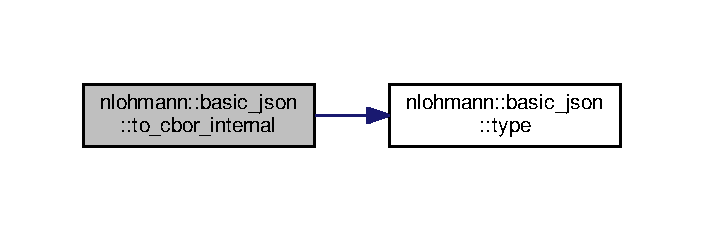
\includegraphics[width=338pt]{classnlohmann_1_1basic__json_a2f208f86f3fafaa8e9bc9374963485e4_cgraph}
\end{center}
\end{figure}
\mbox{\Hypertarget{classnlohmann_1_1basic__json_a09ca1dc273d226afe0ca83a9d7438d9c}\label{classnlohmann_1_1basic__json_a09ca1dc273d226afe0ca83a9d7438d9c}} 
\index{nlohmann\+::basic\+\_\+json@{nlohmann\+::basic\+\_\+json}!to\+\_\+msgpack@{to\+\_\+msgpack}}
\index{to\+\_\+msgpack@{to\+\_\+msgpack}!nlohmann\+::basic\+\_\+json@{nlohmann\+::basic\+\_\+json}}
\subsubsection{\texorpdfstring{to\+\_\+msgpack()}{to\_msgpack()}}
{\footnotesize\ttfamily template$<$template$<$ typename U, typename V, typename... Args $>$ class Object\+Type = std\+::map, template$<$ typename U, typename... Args $>$ class Array\+Type = std\+::vector, class String\+Type  = std\+::string, class Boolean\+Type  = bool, class Number\+Integer\+Type  = std\+::int64\+\_\+t, class Number\+Unsigned\+Type  = std\+::uint64\+\_\+t, class Number\+Float\+Type  = double, template$<$ typename U $>$ class Allocator\+Type = std\+::allocator, template$<$ typename T, typename S\+F\+I\+N\+A\+E=void $>$ class J\+S\+O\+N\+Serializer = adl\+\_\+serializer$>$ \\
static std\+::vector$<$uint8\+\_\+t$>$ \hyperlink{classnlohmann_1_1basic__json}{nlohmann\+::basic\+\_\+json}$<$ Object\+Type, Array\+Type, String\+Type, Boolean\+Type, Number\+Integer\+Type, Number\+Unsigned\+Type, Number\+Float\+Type, Allocator\+Type, J\+S\+O\+N\+Serializer $>$\+::to\+\_\+msgpack (\begin{DoxyParamCaption}\item[{const \hyperlink{classnlohmann_1_1basic__json}{basic\+\_\+json}$<$ Object\+Type, Array\+Type, String\+Type, Boolean\+Type, Number\+Integer\+Type, Number\+Unsigned\+Type, Number\+Float\+Type, Allocator\+Type, J\+S\+O\+N\+Serializer $>$ \&}]{j }\end{DoxyParamCaption})\hspace{0.3cm}{\ttfamily [inline]}, {\ttfamily [static]}}



create a Message\+Pack serialization of a given J\+S\+ON value 

Serializes a given J\+S\+ON value {\itshape j} to a byte vector using the Message\+Pack serialization format. Message\+Pack is a binary serialization format which aims to be more compact than J\+S\+ON itself, yet more efficient to parse.


\begin{DoxyParams}[1]{Parameters}
\mbox{\tt in}  & {\em j} & J\+S\+ON value to serialize \\
\hline
\end{DoxyParams}
\begin{DoxyReturn}{Returns}
Message\+Pack serialization as byte vector
\end{DoxyReturn}
Linear in the size of the J\+S\+ON value {\itshape j}.

\{The example shows the serialization of a J\+S\+ON value to a byte vector in Message\+Pack format.,to\+\_\+msgpack\}

\begin{DoxySeeAlso}{See also}
\href{http://msgpack.org}{\tt http\+://msgpack.\+org} 

\hyperlink{classnlohmann_1_1basic__json_a3eafe0b1fb2f2c443f1b3fea55c8a470}{from\+\_\+msgpack(const std\+::vector$<$uint8\+\_\+t$>$\&, const size\+\_\+t)} for the analogous deserialization 

\hyperlink{classnlohmann_1_1basic__json_a2566783e190dec524bf3445b322873b8}{to\+\_\+cbor}(const \hyperlink{classnlohmann_1_1basic__json}{basic\+\_\+json}\& for the related C\+B\+OR format
\end{DoxySeeAlso}
\begin{DoxySince}{Since}
version 2.\+0.\+9 
\end{DoxySince}
\mbox{\Hypertarget{classnlohmann_1_1basic__json_af7b03056b7891c59fee1811756b1a856}\label{classnlohmann_1_1basic__json_af7b03056b7891c59fee1811756b1a856}} 
\index{nlohmann\+::basic\+\_\+json@{nlohmann\+::basic\+\_\+json}!to\+\_\+msgpack\+\_\+internal@{to\+\_\+msgpack\+\_\+internal}}
\index{to\+\_\+msgpack\+\_\+internal@{to\+\_\+msgpack\+\_\+internal}!nlohmann\+::basic\+\_\+json@{nlohmann\+::basic\+\_\+json}}
\subsubsection{\texorpdfstring{to\+\_\+msgpack\+\_\+internal()}{to\_msgpack\_internal()}}
{\footnotesize\ttfamily template$<$template$<$ typename U, typename V, typename... Args $>$ class Object\+Type = std\+::map, template$<$ typename U, typename... Args $>$ class Array\+Type = std\+::vector, class String\+Type  = std\+::string, class Boolean\+Type  = bool, class Number\+Integer\+Type  = std\+::int64\+\_\+t, class Number\+Unsigned\+Type  = std\+::uint64\+\_\+t, class Number\+Float\+Type  = double, template$<$ typename U $>$ class Allocator\+Type = std\+::allocator, template$<$ typename T, typename S\+F\+I\+N\+A\+E=void $>$ class J\+S\+O\+N\+Serializer = adl\+\_\+serializer$>$ \\
static void \hyperlink{classnlohmann_1_1basic__json}{nlohmann\+::basic\+\_\+json}$<$ Object\+Type, Array\+Type, String\+Type, Boolean\+Type, Number\+Integer\+Type, Number\+Unsigned\+Type, Number\+Float\+Type, Allocator\+Type, J\+S\+O\+N\+Serializer $>$\+::to\+\_\+msgpack\+\_\+internal (\begin{DoxyParamCaption}\item[{const \hyperlink{classnlohmann_1_1basic__json}{basic\+\_\+json}$<$ Object\+Type, Array\+Type, String\+Type, Boolean\+Type, Number\+Integer\+Type, Number\+Unsigned\+Type, Number\+Float\+Type, Allocator\+Type, J\+S\+O\+N\+Serializer $>$ \&}]{j,  }\item[{std\+::vector$<$ uint8\+\_\+t $>$ \&}]{v }\end{DoxyParamCaption})\hspace{0.3cm}{\ttfamily [inline]}, {\ttfamily [static]}, {\ttfamily [private]}}



create a Message\+Pack serialization of a given J\+S\+ON value 

This is a straightforward implementation of the Message\+Pack specification.


\begin{DoxyParams}[1]{Parameters}
\mbox{\tt in}  & {\em j} & J\+S\+ON value to serialize \\
\hline
\mbox{\tt in,out}  & {\em v} & byte vector to write the serialization to\\
\hline
\end{DoxyParams}
\begin{DoxySeeAlso}{See also}
\href{https://github.com/msgpack/msgpack/blob/master/spec.md}{\tt https\+://github.\+com/msgpack/msgpack/blob/master/spec.\+md} 
\end{DoxySeeAlso}
Here is the call graph for this function\+:\nopagebreak
\begin{figure}[H]
\begin{center}
\leavevmode
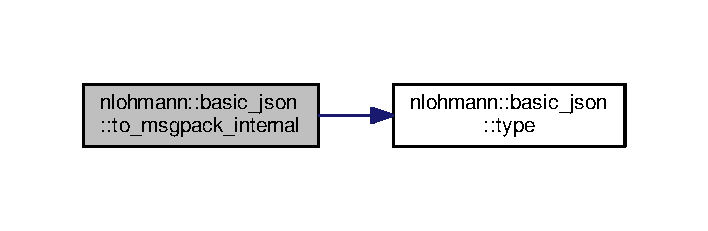
\includegraphics[width=340pt]{classnlohmann_1_1basic__json_af7b03056b7891c59fee1811756b1a856_cgraph}
\end{center}
\end{figure}
\mbox{\Hypertarget{classnlohmann_1_1basic__json_a2b2d781d7f2a4ee41bc0016e931cadf7}\label{classnlohmann_1_1basic__json_a2b2d781d7f2a4ee41bc0016e931cadf7}} 
\index{nlohmann\+::basic\+\_\+json@{nlohmann\+::basic\+\_\+json}!type@{type}}
\index{type@{type}!nlohmann\+::basic\+\_\+json@{nlohmann\+::basic\+\_\+json}}
\subsubsection{\texorpdfstring{type()}{type()}}
{\footnotesize\ttfamily template$<$template$<$ typename U, typename V, typename... Args $>$ class Object\+Type = std\+::map, template$<$ typename U, typename... Args $>$ class Array\+Type = std\+::vector, class String\+Type  = std\+::string, class Boolean\+Type  = bool, class Number\+Integer\+Type  = std\+::int64\+\_\+t, class Number\+Unsigned\+Type  = std\+::uint64\+\_\+t, class Number\+Float\+Type  = double, template$<$ typename U $>$ class Allocator\+Type = std\+::allocator, template$<$ typename T, typename S\+F\+I\+N\+A\+E=void $>$ class J\+S\+O\+N\+Serializer = adl\+\_\+serializer$>$ \\
constexpr \hyperlink{namespacenlohmann_1_1detail_a90aa5ef615aa8305e9ea20d8a947980f}{value\+\_\+t} \hyperlink{classnlohmann_1_1basic__json}{nlohmann\+::basic\+\_\+json}$<$ Object\+Type, Array\+Type, String\+Type, Boolean\+Type, Number\+Integer\+Type, Number\+Unsigned\+Type, Number\+Float\+Type, Allocator\+Type, J\+S\+O\+N\+Serializer $>$\+::type (\begin{DoxyParamCaption}{ }\end{DoxyParamCaption}) const\hspace{0.3cm}{\ttfamily [inline]}, {\ttfamily [noexcept]}}



return the type of the J\+S\+ON value (explicit) 

Return the type of the J\+S\+ON value as a value from the \hyperlink{classnlohmann_1_1basic__json_ae8cbef097f7da18a781fc86587de6b90}{value\+\_\+t} enumeration.

\begin{DoxyReturn}{Returns}
the type of the J\+S\+ON value
\end{DoxyReturn}
Constant.

No-\/throw guarantee\+: this member function never throws exceptions.

\{The following code exemplifies {\ttfamily \hyperlink{classnlohmann_1_1basic__json_a2b2d781d7f2a4ee41bc0016e931cadf7}{type()}} for all J\+S\+ON types.,type\}

\begin{DoxySince}{Since}
version 1.\+0.\+0 
\end{DoxySince}
\mbox{\Hypertarget{classnlohmann_1_1basic__json_a6b75862bdb4d26650616cf9821430755}\label{classnlohmann_1_1basic__json_a6b75862bdb4d26650616cf9821430755}} 
\index{nlohmann\+::basic\+\_\+json@{nlohmann\+::basic\+\_\+json}!type\+\_\+name@{type\+\_\+name}}
\index{type\+\_\+name@{type\+\_\+name}!nlohmann\+::basic\+\_\+json@{nlohmann\+::basic\+\_\+json}}
\subsubsection{\texorpdfstring{type\+\_\+name()}{type\_name()}}
{\footnotesize\ttfamily template$<$template$<$ typename U, typename V, typename... Args $>$ class Object\+Type = std\+::map, template$<$ typename U, typename... Args $>$ class Array\+Type = std\+::vector, class String\+Type  = std\+::string, class Boolean\+Type  = bool, class Number\+Integer\+Type  = std\+::int64\+\_\+t, class Number\+Unsigned\+Type  = std\+::uint64\+\_\+t, class Number\+Float\+Type  = double, template$<$ typename U $>$ class Allocator\+Type = std\+::allocator, template$<$ typename T, typename S\+F\+I\+N\+A\+E=void $>$ class J\+S\+O\+N\+Serializer = adl\+\_\+serializer$>$ \\
std\+::string \hyperlink{classnlohmann_1_1basic__json}{nlohmann\+::basic\+\_\+json}$<$ Object\+Type, Array\+Type, String\+Type, Boolean\+Type, Number\+Integer\+Type, Number\+Unsigned\+Type, Number\+Float\+Type, Allocator\+Type, J\+S\+O\+N\+Serializer $>$\+::type\+\_\+name (\begin{DoxyParamCaption}{ }\end{DoxyParamCaption}) const\hspace{0.3cm}{\ttfamily [inline]}}



return the type as string 

Returns the type name as string to be used in error messages -\/ usually to indicate that a function was called on a wrong J\+S\+ON type.

\begin{DoxyReturn}{Returns}
basically a string representation of a the {\itshape m\+\_\+type} member
\end{DoxyReturn}
Constant.

\{The following code exemplifies {\ttfamily \hyperlink{classnlohmann_1_1basic__json_a6b75862bdb4d26650616cf9821430755}{type\+\_\+name()}} for all J\+S\+ON types.,type\+\_\+name\}

\begin{DoxySince}{Since}
version 1.\+0.\+0, public since 2.\+1.\+0 
\end{DoxySince}
\mbox{\Hypertarget{classnlohmann_1_1basic__json_a74fa3ab2003f2f6f2b69deaafed9126d}\label{classnlohmann_1_1basic__json_a74fa3ab2003f2f6f2b69deaafed9126d}} 
\index{nlohmann\+::basic\+\_\+json@{nlohmann\+::basic\+\_\+json}!unflatten@{unflatten}}
\index{unflatten@{unflatten}!nlohmann\+::basic\+\_\+json@{nlohmann\+::basic\+\_\+json}}
\subsubsection{\texorpdfstring{unflatten()}{unflatten()}}
{\footnotesize\ttfamily template$<$template$<$ typename U, typename V, typename... Args $>$ class Object\+Type = std\+::map, template$<$ typename U, typename... Args $>$ class Array\+Type = std\+::vector, class String\+Type  = std\+::string, class Boolean\+Type  = bool, class Number\+Integer\+Type  = std\+::int64\+\_\+t, class Number\+Unsigned\+Type  = std\+::uint64\+\_\+t, class Number\+Float\+Type  = double, template$<$ typename U $>$ class Allocator\+Type = std\+::allocator, template$<$ typename T, typename S\+F\+I\+N\+A\+E=void $>$ class J\+S\+O\+N\+Serializer = adl\+\_\+serializer$>$ \\
\hyperlink{classnlohmann_1_1basic__json}{basic\+\_\+json} \hyperlink{classnlohmann_1_1basic__json}{nlohmann\+::basic\+\_\+json}$<$ Object\+Type, Array\+Type, String\+Type, Boolean\+Type, Number\+Integer\+Type, Number\+Unsigned\+Type, Number\+Float\+Type, Allocator\+Type, J\+S\+O\+N\+Serializer $>$\+::unflatten (\begin{DoxyParamCaption}{ }\end{DoxyParamCaption}) const\hspace{0.3cm}{\ttfamily [inline]}}



unflatten a previously flattened J\+S\+ON value 

The function restores the arbitrary nesting of a J\+S\+ON value that has been flattened before using the \hyperlink{classnlohmann_1_1basic__json_ab838f000d76662917ffd6ec529569e03}{flatten()} function. The J\+S\+ON value must meet certain constraints\+:
\begin{DoxyEnumerate}
\item The value must be an object.
\item The keys must be J\+S\+ON pointers (see \href{https://tools.ietf.org/html/rfc6901}{\tt R\+FC 6901})
\item The mapped values must be primitive J\+S\+ON types.
\end{DoxyEnumerate}

\begin{DoxyReturn}{Returns}
the original J\+S\+ON from a flattened version
\end{DoxyReturn}
\begin{DoxyNote}{Note}
Empty objects and arrays are flattened by \hyperlink{classnlohmann_1_1basic__json_ab838f000d76662917ffd6ec529569e03}{flatten()} to {\ttfamily null} values and can not unflattened to their original type. Apart from this example, for a J\+S\+ON value {\ttfamily j}, the following is always true\+: {\ttfamily j == j.\+flatten().\hyperlink{classnlohmann_1_1basic__json_a74fa3ab2003f2f6f2b69deaafed9126d}{unflatten()}}.
\end{DoxyNote}
Linear in the size the J\+S\+ON value.

\{The following code shows how a flattened J\+S\+ON object is unflattened into the original nested J\+S\+ON object.,unflatten\}

\begin{DoxySeeAlso}{See also}
\hyperlink{classnlohmann_1_1basic__json_ab838f000d76662917ffd6ec529569e03}{flatten()} for the reverse function
\end{DoxySeeAlso}
\begin{DoxySince}{Since}
version 2.\+0.\+0 
\end{DoxySince}
\mbox{\Hypertarget{classnlohmann_1_1basic__json_af9c51328fbe1da75eca750be3009917a}\label{classnlohmann_1_1basic__json_af9c51328fbe1da75eca750be3009917a}} 
\index{nlohmann\+::basic\+\_\+json@{nlohmann\+::basic\+\_\+json}!value@{value}}
\index{value@{value}!nlohmann\+::basic\+\_\+json@{nlohmann\+::basic\+\_\+json}}
\subsubsection{\texorpdfstring{value()}{value()}\hspace{0.1cm}{\footnotesize\ttfamily [1/4]}}
{\footnotesize\ttfamily template$<$template$<$ typename U, typename V, typename... Args $>$ class Object\+Type = std\+::map, template$<$ typename U, typename... Args $>$ class Array\+Type = std\+::vector, class String\+Type  = std\+::string, class Boolean\+Type  = bool, class Number\+Integer\+Type  = std\+::int64\+\_\+t, class Number\+Unsigned\+Type  = std\+::uint64\+\_\+t, class Number\+Float\+Type  = double, template$<$ typename U $>$ class Allocator\+Type = std\+::allocator, template$<$ typename T, typename S\+F\+I\+N\+A\+E=void $>$ class J\+S\+O\+N\+Serializer = adl\+\_\+serializer$>$ \\
template$<$class Value\+Type , typename std\+::enable\+\_\+if$<$ std\+::is\+\_\+convertible$<$ basic\+\_\+json\+\_\+t, Value\+Type $>$\+::value, int $>$\+::type  = 0$>$ \\
Value\+Type \hyperlink{classnlohmann_1_1basic__json}{nlohmann\+::basic\+\_\+json}$<$ Object\+Type, Array\+Type, String\+Type, Boolean\+Type, Number\+Integer\+Type, Number\+Unsigned\+Type, Number\+Float\+Type, Allocator\+Type, J\+S\+O\+N\+Serializer $>$\+::value (\begin{DoxyParamCaption}\item[{const typename object\+\_\+t\+::key\+\_\+type \&}]{key,  }\item[{Value\+Type}]{default\+\_\+value }\end{DoxyParamCaption}) const\hspace{0.3cm}{\ttfamily [inline]}}



access specified object element with default value 

Returns either a copy of an object\textquotesingle{}s element at the specified key {\itshape key} or a given default value if no element with key {\itshape key} exists.

The function is basically equivalent to executing 
\begin{DoxyCode}
\textcolor{keywordflow}{try} \{
    \textcolor{keywordflow}{return} \hyperlink{classnlohmann_1_1basic__json_a73ae333487310e3302135189ce8ff5d8}{at}(key);
\} \textcolor{keywordflow}{catch}(std::out\_of\_range) \{
    \textcolor{keywordflow}{return} default\_value;
\}
\end{DoxyCode}


\begin{DoxyNote}{Note}
Unlike \hyperlink{classnlohmann_1_1basic__json_a93403e803947b86f4da2d1fb3345cf2c}{at(const typename object\+\_\+t\+::key\+\_\+type\&)}, this function does not throw if the given key {\itshape key} was not found.

Unlike \hyperlink{classnlohmann_1_1basic__json_a233b02b0839ef798942dd46157cc0fe6}{operator\mbox{[}$\,$\mbox{]}(const typename object\+\_\+t\+::key\+\_\+type\& key)}, this function does not implicitly add an element to the position defined by {\itshape key}. This function is furthermore also applicable to const objects.
\end{DoxyNote}

\begin{DoxyParams}[1]{Parameters}
\mbox{\tt in}  & {\em key} & key of the element to access \\
\hline
\mbox{\tt in}  & {\em default\+\_\+value} & the value to return if {\itshape key} is not found\\
\hline
\end{DoxyParams}

\begin{DoxyTemplParams}{Template Parameters}
{\em Value\+Type} & type compatible to J\+S\+ON values, for instance {\ttfamily int} for J\+S\+ON integer numbers, {\ttfamily bool} for J\+S\+ON booleans, or {\ttfamily std\+::vector} types for J\+S\+ON arrays. Note the type of the expected value at {\itshape key} and the default value {\itshape default\+\_\+value} must be compatible.\\
\hline
\end{DoxyTemplParams}
\begin{DoxyReturn}{Returns}
copy of the element at key {\itshape key} or {\itshape default\+\_\+value} if {\itshape key} is not found
\end{DoxyReturn}

\begin{DoxyExceptions}{Exceptions}
{\em std\+::domain\+\_\+error} & if J\+S\+ON is not an object; example\+: {\ttfamily \char`\"{}cannot use
value() with null\char`\"{}}\\
\hline
\end{DoxyExceptions}
Logarithmic in the size of the container.

\{The example below shows how object elements can be queried with a default value.,basic\+\_\+json\+\_\+\+\_\+value\}

\begin{DoxySeeAlso}{See also}
\hyperlink{classnlohmann_1_1basic__json_a93403e803947b86f4da2d1fb3345cf2c}{at(const typename object\+\_\+t\+::key\+\_\+type\&)} for access by \hyperlink{classnlohmann_1_1basic__json_ac6a5eddd156c776ac75ff54cfe54a5bc}{reference} with range checking 

\hyperlink{classnlohmann_1_1basic__json_a233b02b0839ef798942dd46157cc0fe6}{operator\mbox{[}$\,$\mbox{]}(const typename object\+\_\+t\+::key\+\_\+type\&)} for unchecked access by \hyperlink{classnlohmann_1_1basic__json_ac6a5eddd156c776ac75ff54cfe54a5bc}{reference}
\end{DoxySeeAlso}
\begin{DoxySince}{Since}
version 1.\+0.\+0 
\end{DoxySince}
\mbox{\Hypertarget{classnlohmann_1_1basic__json_ad6a18403e7fbac9c4efd06facc71fc88}\label{classnlohmann_1_1basic__json_ad6a18403e7fbac9c4efd06facc71fc88}} 
\index{nlohmann\+::basic\+\_\+json@{nlohmann\+::basic\+\_\+json}!value@{value}}
\index{value@{value}!nlohmann\+::basic\+\_\+json@{nlohmann\+::basic\+\_\+json}}
\subsubsection{\texorpdfstring{value()}{value()}\hspace{0.1cm}{\footnotesize\ttfamily [2/4]}}
{\footnotesize\ttfamily template$<$template$<$ typename U, typename V, typename... Args $>$ class Object\+Type = std\+::map, template$<$ typename U, typename... Args $>$ class Array\+Type = std\+::vector, class String\+Type  = std\+::string, class Boolean\+Type  = bool, class Number\+Integer\+Type  = std\+::int64\+\_\+t, class Number\+Unsigned\+Type  = std\+::uint64\+\_\+t, class Number\+Float\+Type  = double, template$<$ typename U $>$ class Allocator\+Type = std\+::allocator, template$<$ typename T, typename S\+F\+I\+N\+A\+E=void $>$ class J\+S\+O\+N\+Serializer = adl\+\_\+serializer$>$ \\
\hyperlink{classnlohmann_1_1basic__json_a61f8566a1a85a424c7266fb531dca005}{string\+\_\+t} \hyperlink{classnlohmann_1_1basic__json}{nlohmann\+::basic\+\_\+json}$<$ Object\+Type, Array\+Type, String\+Type, Boolean\+Type, Number\+Integer\+Type, Number\+Unsigned\+Type, Number\+Float\+Type, Allocator\+Type, J\+S\+O\+N\+Serializer $>$\+::value (\begin{DoxyParamCaption}\item[{const typename object\+\_\+t\+::key\+\_\+type \&}]{key,  }\item[{const char $\ast$}]{default\+\_\+value }\end{DoxyParamCaption}) const\hspace{0.3cm}{\ttfamily [inline]}}



overload for a default value of type const char$\ast$ 

access specified object element with default value Returns either a copy of an object\textquotesingle{}s element at the specified key {\itshape key} or a given default value if no element with key {\itshape key} exists.

The function is basically equivalent to executing 
\begin{DoxyCode}
\textcolor{keywordflow}{try} \{
    \textcolor{keywordflow}{return} \hyperlink{classnlohmann_1_1basic__json_a73ae333487310e3302135189ce8ff5d8}{at}(key);
\} \textcolor{keywordflow}{catch}(std::out\_of\_range) \{
    \textcolor{keywordflow}{return} default\_value;
\}
\end{DoxyCode}


\begin{DoxyNote}{Note}
Unlike \hyperlink{classnlohmann_1_1basic__json_a93403e803947b86f4da2d1fb3345cf2c}{at(const typename object\+\_\+t\+::key\+\_\+type\&)}, this function does not throw if the given key {\itshape key} was not found.

Unlike \hyperlink{classnlohmann_1_1basic__json_a233b02b0839ef798942dd46157cc0fe6}{operator\mbox{[}$\,$\mbox{]}(const typename object\+\_\+t\+::key\+\_\+type\& key)}, this function does not implicitly add an element to the position defined by {\itshape key}. This function is furthermore also applicable to const objects.
\end{DoxyNote}

\begin{DoxyParams}[1]{Parameters}
\mbox{\tt in}  & {\em key} & key of the element to access \\
\hline
\mbox{\tt in}  & {\em default\+\_\+value} & the value to return if {\itshape key} is not found\\
\hline
\end{DoxyParams}

\begin{DoxyTemplParams}{Template Parameters}
{\em Value\+Type} & type compatible to J\+S\+ON values, for instance {\ttfamily int} for J\+S\+ON integer numbers, {\ttfamily bool} for J\+S\+ON booleans, or {\ttfamily std\+::vector} types for J\+S\+ON arrays. Note the type of the expected value at {\itshape key} and the default value {\itshape default\+\_\+value} must be compatible.\\
\hline
\end{DoxyTemplParams}
\begin{DoxyReturn}{Returns}
copy of the element at key {\itshape key} or {\itshape default\+\_\+value} if {\itshape key} is not found
\end{DoxyReturn}

\begin{DoxyExceptions}{Exceptions}
{\em std\+::domain\+\_\+error} & if J\+S\+ON is not an object; example\+: {\ttfamily \char`\"{}cannot use
value() with null\char`\"{}}\\
\hline
\end{DoxyExceptions}
Logarithmic in the size of the container.

\{The example below shows how object elements can be queried with a default value.,basic\+\_\+json\+\_\+\+\_\+value\}

\begin{DoxySeeAlso}{See also}
\hyperlink{classnlohmann_1_1basic__json_a93403e803947b86f4da2d1fb3345cf2c}{at(const typename object\+\_\+t\+::key\+\_\+type\&)} for access by \hyperlink{classnlohmann_1_1basic__json_ac6a5eddd156c776ac75ff54cfe54a5bc}{reference} with range checking 

\hyperlink{classnlohmann_1_1basic__json_a233b02b0839ef798942dd46157cc0fe6}{operator\mbox{[}$\,$\mbox{]}(const typename object\+\_\+t\+::key\+\_\+type\&)} for unchecked access by \hyperlink{classnlohmann_1_1basic__json_ac6a5eddd156c776ac75ff54cfe54a5bc}{reference}
\end{DoxySeeAlso}
\begin{DoxySince}{Since}
version 1.\+0.\+0 
\end{DoxySince}
\mbox{\Hypertarget{classnlohmann_1_1basic__json_ab7df4291dda0a80d86f74427cc3993ba}\label{classnlohmann_1_1basic__json_ab7df4291dda0a80d86f74427cc3993ba}} 
\index{nlohmann\+::basic\+\_\+json@{nlohmann\+::basic\+\_\+json}!value@{value}}
\index{value@{value}!nlohmann\+::basic\+\_\+json@{nlohmann\+::basic\+\_\+json}}
\subsubsection{\texorpdfstring{value()}{value()}\hspace{0.1cm}{\footnotesize\ttfamily [3/4]}}
{\footnotesize\ttfamily template$<$template$<$ typename U, typename V, typename... Args $>$ class Object\+Type = std\+::map, template$<$ typename U, typename... Args $>$ class Array\+Type = std\+::vector, class String\+Type  = std\+::string, class Boolean\+Type  = bool, class Number\+Integer\+Type  = std\+::int64\+\_\+t, class Number\+Unsigned\+Type  = std\+::uint64\+\_\+t, class Number\+Float\+Type  = double, template$<$ typename U $>$ class Allocator\+Type = std\+::allocator, template$<$ typename T, typename S\+F\+I\+N\+A\+E=void $>$ class J\+S\+O\+N\+Serializer = adl\+\_\+serializer$>$ \\
template$<$class Value\+Type , typename std\+::enable\+\_\+if$<$ std\+::is\+\_\+convertible$<$ basic\+\_\+json\+\_\+t, Value\+Type $>$\+::value, int $>$\+::type  = 0$>$ \\
Value\+Type \hyperlink{classnlohmann_1_1basic__json}{nlohmann\+::basic\+\_\+json}$<$ Object\+Type, Array\+Type, String\+Type, Boolean\+Type, Number\+Integer\+Type, Number\+Unsigned\+Type, Number\+Float\+Type, Allocator\+Type, J\+S\+O\+N\+Serializer $>$\+::value (\begin{DoxyParamCaption}\item[{const \hyperlink{classnlohmann_1_1basic__json_1_1json__pointer}{json\+\_\+pointer} \&}]{ptr,  }\item[{Value\+Type}]{default\+\_\+value }\end{DoxyParamCaption}) const\hspace{0.3cm}{\ttfamily [inline]}}



access specified object element via J\+S\+ON Pointer with default value 

Returns either a copy of an object\textquotesingle{}s element at the specified key {\itshape key} or a given default value if no element with key {\itshape key} exists.

The function is basically equivalent to executing 
\begin{DoxyCode}
\textcolor{keywordflow}{try} \{
    \textcolor{keywordflow}{return} \hyperlink{classnlohmann_1_1basic__json_a73ae333487310e3302135189ce8ff5d8}{at}(ptr);
\} \textcolor{keywordflow}{catch}(std::out\_of\_range) \{
    \textcolor{keywordflow}{return} default\_value;
\}
\end{DoxyCode}


\begin{DoxyNote}{Note}
Unlike \hyperlink{classnlohmann_1_1basic__json_a8ab61397c10f18b305520da7073b2b45}{at(const json\+\_\+pointer\&)}, this function does not throw if the given key {\itshape key} was not found.
\end{DoxyNote}

\begin{DoxyParams}[1]{Parameters}
\mbox{\tt in}  & {\em ptr} & a J\+S\+ON pointer to the element to access \\
\hline
\mbox{\tt in}  & {\em default\+\_\+value} & the value to return if {\itshape ptr} found no value\\
\hline
\end{DoxyParams}

\begin{DoxyTemplParams}{Template Parameters}
{\em Value\+Type} & type compatible to J\+S\+ON values, for instance {\ttfamily int} for J\+S\+ON integer numbers, {\ttfamily bool} for J\+S\+ON booleans, or {\ttfamily std\+::vector} types for J\+S\+ON arrays. Note the type of the expected value at {\itshape key} and the default value {\itshape default\+\_\+value} must be compatible.\\
\hline
\end{DoxyTemplParams}
\begin{DoxyReturn}{Returns}
copy of the element at key {\itshape key} or {\itshape default\+\_\+value} if {\itshape key} is not found
\end{DoxyReturn}

\begin{DoxyExceptions}{Exceptions}
{\em std\+::domain\+\_\+error} & if J\+S\+ON is not an object; example\+: {\ttfamily \char`\"{}cannot use
value() with null\char`\"{}}\\
\hline
\end{DoxyExceptions}
Logarithmic in the size of the container.

\{The example below shows how object elements can be queried with a default value.,basic\+\_\+json\+\_\+\+\_\+value\+\_\+ptr\}

\begin{DoxySeeAlso}{See also}
\hyperlink{classnlohmann_1_1basic__json_ac6946dffeb3be5aa173645f0467a44b3}{operator\mbox{[}$\,$\mbox{]}(const json\+\_\+pointer\&)} for unchecked access by \hyperlink{classnlohmann_1_1basic__json_ac6a5eddd156c776ac75ff54cfe54a5bc}{reference}
\end{DoxySeeAlso}
\begin{DoxySince}{Since}
version 2.\+0.\+2 
\end{DoxySince}
Here is the call graph for this function\+:\nopagebreak
\begin{figure}[H]
\begin{center}
\leavevmode
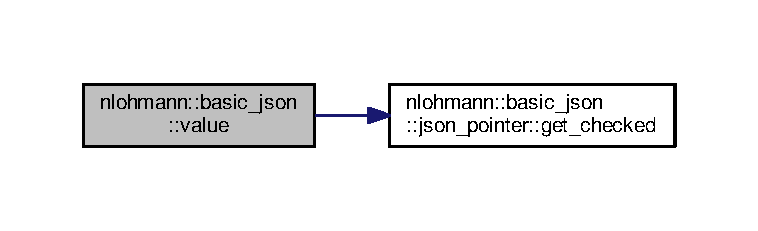
\includegraphics[width=350pt]{classnlohmann_1_1basic__json_ab7df4291dda0a80d86f74427cc3993ba_cgraph}
\end{center}
\end{figure}
\mbox{\Hypertarget{classnlohmann_1_1basic__json_a869c900ee02cf1a68988dcce3b375424}\label{classnlohmann_1_1basic__json_a869c900ee02cf1a68988dcce3b375424}} 
\index{nlohmann\+::basic\+\_\+json@{nlohmann\+::basic\+\_\+json}!value@{value}}
\index{value@{value}!nlohmann\+::basic\+\_\+json@{nlohmann\+::basic\+\_\+json}}
\subsubsection{\texorpdfstring{value()}{value()}\hspace{0.1cm}{\footnotesize\ttfamily [4/4]}}
{\footnotesize\ttfamily template$<$template$<$ typename U, typename V, typename... Args $>$ class Object\+Type = std\+::map, template$<$ typename U, typename... Args $>$ class Array\+Type = std\+::vector, class String\+Type  = std\+::string, class Boolean\+Type  = bool, class Number\+Integer\+Type  = std\+::int64\+\_\+t, class Number\+Unsigned\+Type  = std\+::uint64\+\_\+t, class Number\+Float\+Type  = double, template$<$ typename U $>$ class Allocator\+Type = std\+::allocator, template$<$ typename T, typename S\+F\+I\+N\+A\+E=void $>$ class J\+S\+O\+N\+Serializer = adl\+\_\+serializer$>$ \\
\hyperlink{classnlohmann_1_1basic__json_a61f8566a1a85a424c7266fb531dca005}{string\+\_\+t} \hyperlink{classnlohmann_1_1basic__json}{nlohmann\+::basic\+\_\+json}$<$ Object\+Type, Array\+Type, String\+Type, Boolean\+Type, Number\+Integer\+Type, Number\+Unsigned\+Type, Number\+Float\+Type, Allocator\+Type, J\+S\+O\+N\+Serializer $>$\+::value (\begin{DoxyParamCaption}\item[{const \hyperlink{classnlohmann_1_1basic__json_1_1json__pointer}{json\+\_\+pointer} \&}]{ptr,  }\item[{const char $\ast$}]{default\+\_\+value }\end{DoxyParamCaption}) const\hspace{0.3cm}{\ttfamily [inline]}}



overload for a default value of type const char$\ast$ 

access specified object element via J\+S\+ON Pointer with default value Returns either a copy of an object\textquotesingle{}s element at the specified key {\itshape key} or a given default value if no element with key {\itshape key} exists.

The function is basically equivalent to executing 
\begin{DoxyCode}
\textcolor{keywordflow}{try} \{
    \textcolor{keywordflow}{return} \hyperlink{classnlohmann_1_1basic__json_a73ae333487310e3302135189ce8ff5d8}{at}(ptr);
\} \textcolor{keywordflow}{catch}(std::out\_of\_range) \{
    \textcolor{keywordflow}{return} default\_value;
\}
\end{DoxyCode}


\begin{DoxyNote}{Note}
Unlike \hyperlink{classnlohmann_1_1basic__json_a8ab61397c10f18b305520da7073b2b45}{at(const json\+\_\+pointer\&)}, this function does not throw if the given key {\itshape key} was not found.
\end{DoxyNote}

\begin{DoxyParams}[1]{Parameters}
\mbox{\tt in}  & {\em ptr} & a J\+S\+ON pointer to the element to access \\
\hline
\mbox{\tt in}  & {\em default\+\_\+value} & the value to return if {\itshape ptr} found no value\\
\hline
\end{DoxyParams}

\begin{DoxyTemplParams}{Template Parameters}
{\em Value\+Type} & type compatible to J\+S\+ON values, for instance {\ttfamily int} for J\+S\+ON integer numbers, {\ttfamily bool} for J\+S\+ON booleans, or {\ttfamily std\+::vector} types for J\+S\+ON arrays. Note the type of the expected value at {\itshape key} and the default value {\itshape default\+\_\+value} must be compatible.\\
\hline
\end{DoxyTemplParams}
\begin{DoxyReturn}{Returns}
copy of the element at key {\itshape key} or {\itshape default\+\_\+value} if {\itshape key} is not found
\end{DoxyReturn}

\begin{DoxyExceptions}{Exceptions}
{\em std\+::domain\+\_\+error} & if J\+S\+ON is not an object; example\+: {\ttfamily \char`\"{}cannot use
value() with null\char`\"{}}\\
\hline
\end{DoxyExceptions}
Logarithmic in the size of the container.

\{The example below shows how object elements can be queried with a default value.,basic\+\_\+json\+\_\+\+\_\+value\+\_\+ptr\}

\begin{DoxySeeAlso}{See also}
\hyperlink{classnlohmann_1_1basic__json_ac6946dffeb3be5aa173645f0467a44b3}{operator\mbox{[}$\,$\mbox{]}(const json\+\_\+pointer\&)} for unchecked access by \hyperlink{classnlohmann_1_1basic__json_ac6a5eddd156c776ac75ff54cfe54a5bc}{reference}
\end{DoxySeeAlso}
\begin{DoxySince}{Since}
version 2.\+0.\+2 
\end{DoxySince}


\subsection{Friends And Related Function Documentation}
\mbox{\Hypertarget{classnlohmann_1_1basic__json_a6275ed57bae6866cdf5db5370a7ad47c}\label{classnlohmann_1_1basic__json_a6275ed57bae6866cdf5db5370a7ad47c}} 
\index{nlohmann\+::basic\+\_\+json@{nlohmann\+::basic\+\_\+json}!detail\+::external\+\_\+constructor@{detail\+::external\+\_\+constructor}}
\index{detail\+::external\+\_\+constructor@{detail\+::external\+\_\+constructor}!nlohmann\+::basic\+\_\+json@{nlohmann\+::basic\+\_\+json}}
\subsubsection{\texorpdfstring{detail\+::external\+\_\+constructor}{detail::external\_constructor}}
{\footnotesize\ttfamily template$<$template$<$ typename U, typename V, typename... Args $>$ class Object\+Type = std\+::map, template$<$ typename U, typename... Args $>$ class Array\+Type = std\+::vector, class String\+Type  = std\+::string, class Boolean\+Type  = bool, class Number\+Integer\+Type  = std\+::int64\+\_\+t, class Number\+Unsigned\+Type  = std\+::uint64\+\_\+t, class Number\+Float\+Type  = double, template$<$ typename U $>$ class Allocator\+Type = std\+::allocator, template$<$ typename T, typename S\+F\+I\+N\+A\+E=void $>$ class J\+S\+O\+N\+Serializer = adl\+\_\+serializer$>$ \\
template$<$detail\+::value\+\_\+t $>$ \\
friend struct \hyperlink{structnlohmann_1_1detail_1_1external__constructor}{detail\+::external\+\_\+constructor}\hspace{0.3cm}{\ttfamily [friend]}}

\mbox{\Hypertarget{classnlohmann_1_1basic__json_a6e2e21da48f5d9471716cd868a068327}\label{classnlohmann_1_1basic__json_a6e2e21da48f5d9471716cd868a068327}} 
\index{nlohmann\+::basic\+\_\+json@{nlohmann\+::basic\+\_\+json}!operator"!=@{operator"!=}}
\index{operator"!=@{operator"!=}!nlohmann\+::basic\+\_\+json@{nlohmann\+::basic\+\_\+json}}
\subsubsection{\texorpdfstring{operator"!=}{operator!=}\hspace{0.1cm}{\footnotesize\ttfamily [1/3]}}
{\footnotesize\ttfamily template$<$template$<$ typename U, typename V, typename... Args $>$ class Object\+Type = std\+::map, template$<$ typename U, typename... Args $>$ class Array\+Type = std\+::vector, class String\+Type  = std\+::string, class Boolean\+Type  = bool, class Number\+Integer\+Type  = std\+::int64\+\_\+t, class Number\+Unsigned\+Type  = std\+::uint64\+\_\+t, class Number\+Float\+Type  = double, template$<$ typename U $>$ class Allocator\+Type = std\+::allocator, template$<$ typename T, typename S\+F\+I\+N\+A\+E=void $>$ class J\+S\+O\+N\+Serializer = adl\+\_\+serializer$>$ \\
bool operator!= (\begin{DoxyParamCaption}\item[{\hyperlink{classnlohmann_1_1basic__json_a4057c5425f4faacfe39a8046871786ca}{const\+\_\+reference}}]{lhs,  }\item[{\hyperlink{classnlohmann_1_1basic__json_a4057c5425f4faacfe39a8046871786ca}{const\+\_\+reference}}]{rhs }\end{DoxyParamCaption})\hspace{0.3cm}{\ttfamily [friend]}}



comparison\+: not equal 

Compares two J\+S\+ON values for inequality by calculating {\ttfamily not (lhs == rhs)}.


\begin{DoxyParams}[1]{Parameters}
\mbox{\tt in}  & {\em lhs} & first J\+S\+ON value to consider \\
\hline
\mbox{\tt in}  & {\em rhs} & second J\+S\+ON value to consider \\
\hline
\end{DoxyParams}
\begin{DoxyReturn}{Returns}
whether the values {\itshape lhs} and {\itshape rhs} are not equal
\end{DoxyReturn}
Linear.

\{The example demonstrates comparing several J\+S\+ON types.,operator\+\_\+\+\_\+notequal\}

\begin{DoxySince}{Since}
version 1.\+0.\+0 
\end{DoxySince}
\mbox{\Hypertarget{classnlohmann_1_1basic__json_afefc38fc08bdb7a9a7474b5ab4a1140f}\label{classnlohmann_1_1basic__json_afefc38fc08bdb7a9a7474b5ab4a1140f}} 
\index{nlohmann\+::basic\+\_\+json@{nlohmann\+::basic\+\_\+json}!operator"!=@{operator"!=}}
\index{operator"!=@{operator"!=}!nlohmann\+::basic\+\_\+json@{nlohmann\+::basic\+\_\+json}}
\subsubsection{\texorpdfstring{operator"!=}{operator!=}\hspace{0.1cm}{\footnotesize\ttfamily [2/3]}}
{\footnotesize\ttfamily template$<$template$<$ typename U, typename V, typename... Args $>$ class Object\+Type = std\+::map, template$<$ typename U, typename... Args $>$ class Array\+Type = std\+::vector, class String\+Type  = std\+::string, class Boolean\+Type  = bool, class Number\+Integer\+Type  = std\+::int64\+\_\+t, class Number\+Unsigned\+Type  = std\+::uint64\+\_\+t, class Number\+Float\+Type  = double, template$<$ typename U $>$ class Allocator\+Type = std\+::allocator, template$<$ typename T, typename S\+F\+I\+N\+A\+E=void $>$ class J\+S\+O\+N\+Serializer = adl\+\_\+serializer$>$ \\
template$<$typename Scalar\+Type , typename std\+::enable\+\_\+if$<$ std\+::is\+\_\+scalar$<$ Scalar\+Type $>$\+::value, int $>$\+::type  = 0$>$ \\
bool operator!= (\begin{DoxyParamCaption}\item[{\hyperlink{classnlohmann_1_1basic__json_a4057c5425f4faacfe39a8046871786ca}{const\+\_\+reference}}]{lhs,  }\item[{const Scalar\+Type}]{rhs }\end{DoxyParamCaption})\hspace{0.3cm}{\ttfamily [friend]}}



comparison\+: not equal 

comparison\+: not equal Compares two J\+S\+ON values for inequality by calculating {\ttfamily not (lhs == rhs)}.


\begin{DoxyParams}[1]{Parameters}
\mbox{\tt in}  & {\em lhs} & first J\+S\+ON value to consider \\
\hline
\mbox{\tt in}  & {\em rhs} & second J\+S\+ON value to consider \\
\hline
\end{DoxyParams}
\begin{DoxyReturn}{Returns}
whether the values {\itshape lhs} and {\itshape rhs} are not equal
\end{DoxyReturn}
Linear.

\{The example demonstrates comparing several J\+S\+ON types.,operator\+\_\+\+\_\+notequal\}

\begin{DoxySince}{Since}
version 1.\+0.\+0 
\end{DoxySince}
\mbox{\Hypertarget{classnlohmann_1_1basic__json_ab0e886db6e9fa91ff9fd853333fed05b}\label{classnlohmann_1_1basic__json_ab0e886db6e9fa91ff9fd853333fed05b}} 
\index{nlohmann\+::basic\+\_\+json@{nlohmann\+::basic\+\_\+json}!operator"!=@{operator"!=}}
\index{operator"!=@{operator"!=}!nlohmann\+::basic\+\_\+json@{nlohmann\+::basic\+\_\+json}}
\subsubsection{\texorpdfstring{operator"!=}{operator!=}\hspace{0.1cm}{\footnotesize\ttfamily [3/3]}}
{\footnotesize\ttfamily template$<$template$<$ typename U, typename V, typename... Args $>$ class Object\+Type = std\+::map, template$<$ typename U, typename... Args $>$ class Array\+Type = std\+::vector, class String\+Type  = std\+::string, class Boolean\+Type  = bool, class Number\+Integer\+Type  = std\+::int64\+\_\+t, class Number\+Unsigned\+Type  = std\+::uint64\+\_\+t, class Number\+Float\+Type  = double, template$<$ typename U $>$ class Allocator\+Type = std\+::allocator, template$<$ typename T, typename S\+F\+I\+N\+A\+E=void $>$ class J\+S\+O\+N\+Serializer = adl\+\_\+serializer$>$ \\
template$<$typename Scalar\+Type , typename std\+::enable\+\_\+if$<$ std\+::is\+\_\+scalar$<$ Scalar\+Type $>$\+::value, int $>$\+::type  = 0$>$ \\
bool operator!= (\begin{DoxyParamCaption}\item[{const Scalar\+Type}]{lhs,  }\item[{\hyperlink{classnlohmann_1_1basic__json_a4057c5425f4faacfe39a8046871786ca}{const\+\_\+reference}}]{rhs }\end{DoxyParamCaption})\hspace{0.3cm}{\ttfamily [friend]}}



comparison\+: not equal 

comparison\+: not equal Compares two J\+S\+ON values for inequality by calculating {\ttfamily not (lhs == rhs)}.


\begin{DoxyParams}[1]{Parameters}
\mbox{\tt in}  & {\em lhs} & first J\+S\+ON value to consider \\
\hline
\mbox{\tt in}  & {\em rhs} & second J\+S\+ON value to consider \\
\hline
\end{DoxyParams}
\begin{DoxyReturn}{Returns}
whether the values {\itshape lhs} and {\itshape rhs} are not equal
\end{DoxyReturn}
Linear.

\{The example demonstrates comparing several J\+S\+ON types.,operator\+\_\+\+\_\+notequal\}

\begin{DoxySince}{Since}
version 1.\+0.\+0 
\end{DoxySince}
\mbox{\Hypertarget{classnlohmann_1_1basic__json_aacd442b66140c764c594ac8ad7dfd5b3}\label{classnlohmann_1_1basic__json_aacd442b66140c764c594ac8ad7dfd5b3}} 
\index{nlohmann\+::basic\+\_\+json@{nlohmann\+::basic\+\_\+json}!operator$<$@{operator$<$}}
\index{operator$<$@{operator$<$}!nlohmann\+::basic\+\_\+json@{nlohmann\+::basic\+\_\+json}}
\subsubsection{\texorpdfstring{operator$<$}{operator<}}
{\footnotesize\ttfamily template$<$template$<$ typename U, typename V, typename... Args $>$ class Object\+Type = std\+::map, template$<$ typename U, typename... Args $>$ class Array\+Type = std\+::vector, class String\+Type  = std\+::string, class Boolean\+Type  = bool, class Number\+Integer\+Type  = std\+::int64\+\_\+t, class Number\+Unsigned\+Type  = std\+::uint64\+\_\+t, class Number\+Float\+Type  = double, template$<$ typename U $>$ class Allocator\+Type = std\+::allocator, template$<$ typename T, typename S\+F\+I\+N\+A\+E=void $>$ class J\+S\+O\+N\+Serializer = adl\+\_\+serializer$>$ \\
bool operator$<$ (\begin{DoxyParamCaption}\item[{\hyperlink{classnlohmann_1_1basic__json_a4057c5425f4faacfe39a8046871786ca}{const\+\_\+reference}}]{lhs,  }\item[{\hyperlink{classnlohmann_1_1basic__json_a4057c5425f4faacfe39a8046871786ca}{const\+\_\+reference}}]{rhs }\end{DoxyParamCaption})\hspace{0.3cm}{\ttfamily [friend]}}



comparison\+: less than 

Compares whether one J\+S\+ON value {\itshape lhs} is less than another J\+S\+ON value {\itshape rhs} according to the following rules\+:
\begin{DoxyItemize}
\item If {\itshape lhs} and {\itshape rhs} have the same type, the values are compared using the default {\ttfamily $<$} operator.
\item Integer and floating-\/point numbers are automatically converted before comparison
\item In case {\itshape lhs} and {\itshape rhs} have different types, the values are ignored and the order of the types is considered, see operator$<$(const value\+\_\+t, const value\+\_\+t).
\end{DoxyItemize}


\begin{DoxyParams}[1]{Parameters}
\mbox{\tt in}  & {\em lhs} & first J\+S\+ON value to consider \\
\hline
\mbox{\tt in}  & {\em rhs} & second J\+S\+ON value to consider \\
\hline
\end{DoxyParams}
\begin{DoxyReturn}{Returns}
whether {\itshape lhs} is less than {\itshape rhs} 
\end{DoxyReturn}
Linear.

\{The example demonstrates comparing several J\+S\+ON types.,operator\+\_\+\+\_\+less\}

\begin{DoxySince}{Since}
version 1.\+0.\+0 
\end{DoxySince}
\mbox{\Hypertarget{classnlohmann_1_1basic__json_a5e34c5435e557d0bf666bd7311211405}\label{classnlohmann_1_1basic__json_a5e34c5435e557d0bf666bd7311211405}} 
\index{nlohmann\+::basic\+\_\+json@{nlohmann\+::basic\+\_\+json}!operator$<$$<$@{operator$<$$<$}}
\index{operator$<$$<$@{operator$<$$<$}!nlohmann\+::basic\+\_\+json@{nlohmann\+::basic\+\_\+json}}
\subsubsection{\texorpdfstring{operator$<$$<$}{operator<<}\hspace{0.1cm}{\footnotesize\ttfamily [1/2]}}
{\footnotesize\ttfamily template$<$template$<$ typename U, typename V, typename... Args $>$ class Object\+Type = std\+::map, template$<$ typename U, typename... Args $>$ class Array\+Type = std\+::vector, class String\+Type  = std\+::string, class Boolean\+Type  = bool, class Number\+Integer\+Type  = std\+::int64\+\_\+t, class Number\+Unsigned\+Type  = std\+::uint64\+\_\+t, class Number\+Float\+Type  = double, template$<$ typename U $>$ class Allocator\+Type = std\+::allocator, template$<$ typename T, typename S\+F\+I\+N\+A\+E=void $>$ class J\+S\+O\+N\+Serializer = adl\+\_\+serializer$>$ \\
std\+::ostream\& operator$<$$<$ (\begin{DoxyParamCaption}\item[{std\+::ostream \&}]{o,  }\item[{const \hyperlink{classnlohmann_1_1basic__json}{basic\+\_\+json}$<$ Object\+Type, Array\+Type, String\+Type, Boolean\+Type, Number\+Integer\+Type, Number\+Unsigned\+Type, Number\+Float\+Type, Allocator\+Type, J\+S\+O\+N\+Serializer $>$ \&}]{j }\end{DoxyParamCaption})\hspace{0.3cm}{\ttfamily [friend]}}



serialize to stream 

Serialize the given J\+S\+ON value {\itshape j} to the output stream {\itshape o}. The J\+S\+ON value will be serialized using the \hyperlink{classnlohmann_1_1basic__json_a5319dc1bb9dfe19ce7ff559aaded3422}{dump} member function. The indentation of the output can be controlled with the member variable {\ttfamily width} of the output stream {\itshape o}. For instance, using the manipulator {\ttfamily std\+::setw(4)} on {\itshape o} sets the indentation level to {\ttfamily 4} and the serialization result is the same as calling {\ttfamily dump(4)}.


\begin{DoxyParams}[1]{Parameters}
\mbox{\tt in,out}  & {\em o} & stream to serialize to \\
\hline
\mbox{\tt in}  & {\em j} & J\+S\+ON value to serialize\\
\hline
\end{DoxyParams}
\begin{DoxyReturn}{Returns}
the stream {\itshape o} 
\end{DoxyReturn}
Linear.

\{The example below shows the serialization with different parameters to {\ttfamily width} to adjust the indentation level.,operator\+\_\+serialize\}

\begin{DoxySince}{Since}
version 1.\+0.\+0 
\end{DoxySince}
\mbox{\Hypertarget{classnlohmann_1_1basic__json_a60ca396028b8d9714c6e10efbf475af6}\label{classnlohmann_1_1basic__json_a60ca396028b8d9714c6e10efbf475af6}} 
\index{nlohmann\+::basic\+\_\+json@{nlohmann\+::basic\+\_\+json}!operator$<$$<$@{operator$<$$<$}}
\index{operator$<$$<$@{operator$<$$<$}!nlohmann\+::basic\+\_\+json@{nlohmann\+::basic\+\_\+json}}
\subsubsection{\texorpdfstring{operator$<$$<$}{operator<<}\hspace{0.1cm}{\footnotesize\ttfamily [2/2]}}
{\footnotesize\ttfamily template$<$template$<$ typename U, typename V, typename... Args $>$ class Object\+Type = std\+::map, template$<$ typename U, typename... Args $>$ class Array\+Type = std\+::vector, class String\+Type  = std\+::string, class Boolean\+Type  = bool, class Number\+Integer\+Type  = std\+::int64\+\_\+t, class Number\+Unsigned\+Type  = std\+::uint64\+\_\+t, class Number\+Float\+Type  = double, template$<$ typename U $>$ class Allocator\+Type = std\+::allocator, template$<$ typename T, typename S\+F\+I\+N\+A\+E=void $>$ class J\+S\+O\+N\+Serializer = adl\+\_\+serializer$>$ \\
std\+::istream\& operator$<$$<$ (\begin{DoxyParamCaption}\item[{\hyperlink{classnlohmann_1_1basic__json}{basic\+\_\+json}$<$ Object\+Type, Array\+Type, String\+Type, Boolean\+Type, Number\+Integer\+Type, Number\+Unsigned\+Type, Number\+Float\+Type, Allocator\+Type, J\+S\+O\+N\+Serializer $>$ \&}]{j,  }\item[{std\+::istream \&}]{i }\end{DoxyParamCaption})\hspace{0.3cm}{\ttfamily [friend]}}



deserialize from stream 

Deserializes an input stream to a J\+S\+ON value.


\begin{DoxyParams}[1]{Parameters}
\mbox{\tt in,out}  & {\em i} & input stream to read a serialized J\+S\+ON value from \\
\hline
\mbox{\tt in,out}  & {\em j} & J\+S\+ON value to write the deserialized input to\\
\hline
\end{DoxyParams}

\begin{DoxyExceptions}{Exceptions}
{\em std\+::invalid\+\_\+argument} & in case of parse errors\\
\hline
\end{DoxyExceptions}
Linear in the length of the input. The parser is a predictive L\+L(1) parser.

\begin{DoxyNote}{Note}
A U\+T\+F-\/8 byte order mark is silently ignored.
\end{DoxyNote}
\{The example below shows how a J\+S\+ON value is constructed by reading a serialization from a stream.,operator\+\_\+deserialize\}

\begin{DoxySeeAlso}{See also}
\hyperlink{classnlohmann_1_1basic__json_a4cd30efe5c33a7cf73a0c6495bb16054}{parse(std\+::istream\&, const parser\+\_\+callback\+\_\+t)} for a variant with a \hyperlink{classnlohmann_1_1basic__json_1_1parser}{parser} callback function to filter values while parsing
\end{DoxySeeAlso}
\begin{DoxySince}{Since}
version 1.\+0.\+0 
\end{DoxySince}
\mbox{\Hypertarget{classnlohmann_1_1basic__json_a5c8bb5200f5eac10d31e26be46e5b1ac}\label{classnlohmann_1_1basic__json_a5c8bb5200f5eac10d31e26be46e5b1ac}} 
\index{nlohmann\+::basic\+\_\+json@{nlohmann\+::basic\+\_\+json}!operator$<$=@{operator$<$=}}
\index{operator$<$=@{operator$<$=}!nlohmann\+::basic\+\_\+json@{nlohmann\+::basic\+\_\+json}}
\subsubsection{\texorpdfstring{operator$<$=}{operator<=}}
{\footnotesize\ttfamily template$<$template$<$ typename U, typename V, typename... Args $>$ class Object\+Type = std\+::map, template$<$ typename U, typename... Args $>$ class Array\+Type = std\+::vector, class String\+Type  = std\+::string, class Boolean\+Type  = bool, class Number\+Integer\+Type  = std\+::int64\+\_\+t, class Number\+Unsigned\+Type  = std\+::uint64\+\_\+t, class Number\+Float\+Type  = double, template$<$ typename U $>$ class Allocator\+Type = std\+::allocator, template$<$ typename T, typename S\+F\+I\+N\+A\+E=void $>$ class J\+S\+O\+N\+Serializer = adl\+\_\+serializer$>$ \\
bool operator$<$= (\begin{DoxyParamCaption}\item[{\hyperlink{classnlohmann_1_1basic__json_a4057c5425f4faacfe39a8046871786ca}{const\+\_\+reference}}]{lhs,  }\item[{\hyperlink{classnlohmann_1_1basic__json_a4057c5425f4faacfe39a8046871786ca}{const\+\_\+reference}}]{rhs }\end{DoxyParamCaption})\hspace{0.3cm}{\ttfamily [friend]}}



comparison\+: less than or equal 

Compares whether one J\+S\+ON value {\itshape lhs} is less than or equal to another J\+S\+ON value by calculating {\ttfamily not (rhs $<$ lhs)}.


\begin{DoxyParams}[1]{Parameters}
\mbox{\tt in}  & {\em lhs} & first J\+S\+ON value to consider \\
\hline
\mbox{\tt in}  & {\em rhs} & second J\+S\+ON value to consider \\
\hline
\end{DoxyParams}
\begin{DoxyReturn}{Returns}
whether {\itshape lhs} is less than or equal to {\itshape rhs} 
\end{DoxyReturn}
Linear.

\{The example demonstrates comparing several J\+S\+ON types.,operator\+\_\+\+\_\+greater\}

\begin{DoxySince}{Since}
version 1.\+0.\+0 
\end{DoxySince}
\mbox{\Hypertarget{classnlohmann_1_1basic__json_a122640e7e2db1814fc7bbb3c122ec76e}\label{classnlohmann_1_1basic__json_a122640e7e2db1814fc7bbb3c122ec76e}} 
\index{nlohmann\+::basic\+\_\+json@{nlohmann\+::basic\+\_\+json}!operator==@{operator==}}
\index{operator==@{operator==}!nlohmann\+::basic\+\_\+json@{nlohmann\+::basic\+\_\+json}}
\subsubsection{\texorpdfstring{operator==}{operator==}\hspace{0.1cm}{\footnotesize\ttfamily [1/3]}}
{\footnotesize\ttfamily template$<$template$<$ typename U, typename V, typename... Args $>$ class Object\+Type = std\+::map, template$<$ typename U, typename... Args $>$ class Array\+Type = std\+::vector, class String\+Type  = std\+::string, class Boolean\+Type  = bool, class Number\+Integer\+Type  = std\+::int64\+\_\+t, class Number\+Unsigned\+Type  = std\+::uint64\+\_\+t, class Number\+Float\+Type  = double, template$<$ typename U $>$ class Allocator\+Type = std\+::allocator, template$<$ typename T, typename S\+F\+I\+N\+A\+E=void $>$ class J\+S\+O\+N\+Serializer = adl\+\_\+serializer$>$ \\
bool operator== (\begin{DoxyParamCaption}\item[{\hyperlink{classnlohmann_1_1basic__json_a4057c5425f4faacfe39a8046871786ca}{const\+\_\+reference}}]{lhs,  }\item[{\hyperlink{classnlohmann_1_1basic__json_a4057c5425f4faacfe39a8046871786ca}{const\+\_\+reference}}]{rhs }\end{DoxyParamCaption})\hspace{0.3cm}{\ttfamily [friend]}}



comparison\+: equal 

Compares two J\+S\+ON values for equality according to the following rules\+:
\begin{DoxyItemize}
\item Two J\+S\+ON values are equal if (1) they are from the same type and (2) their stored values are the same.
\item Integer and floating-\/point numbers are automatically converted before comparison. Floating-\/point numbers are compared indirectly\+: two floating-\/point numbers {\ttfamily f1} and {\ttfamily f2} are considered equal if neither {\ttfamily f1 $>$ f2} nor {\ttfamily f2 $>$ f1} holds.
\item Two J\+S\+ON null values are equal.
\end{DoxyItemize}


\begin{DoxyParams}[1]{Parameters}
\mbox{\tt in}  & {\em lhs} & first J\+S\+ON value to consider \\
\hline
\mbox{\tt in}  & {\em rhs} & second J\+S\+ON value to consider \\
\hline
\end{DoxyParams}
\begin{DoxyReturn}{Returns}
whether the values {\itshape lhs} and {\itshape rhs} are equal
\end{DoxyReturn}
Linear.

\{The example demonstrates comparing several J\+S\+ON types.,operator\+\_\+\+\_\+equal\}

\begin{DoxySince}{Since}
version 1.\+0.\+0 
\end{DoxySince}
\mbox{\Hypertarget{classnlohmann_1_1basic__json_aba21440ea1aff44f718285ed7d6d20d9}\label{classnlohmann_1_1basic__json_aba21440ea1aff44f718285ed7d6d20d9}} 
\index{nlohmann\+::basic\+\_\+json@{nlohmann\+::basic\+\_\+json}!operator==@{operator==}}
\index{operator==@{operator==}!nlohmann\+::basic\+\_\+json@{nlohmann\+::basic\+\_\+json}}
\subsubsection{\texorpdfstring{operator==}{operator==}\hspace{0.1cm}{\footnotesize\ttfamily [2/3]}}
{\footnotesize\ttfamily template$<$template$<$ typename U, typename V, typename... Args $>$ class Object\+Type = std\+::map, template$<$ typename U, typename... Args $>$ class Array\+Type = std\+::vector, class String\+Type  = std\+::string, class Boolean\+Type  = bool, class Number\+Integer\+Type  = std\+::int64\+\_\+t, class Number\+Unsigned\+Type  = std\+::uint64\+\_\+t, class Number\+Float\+Type  = double, template$<$ typename U $>$ class Allocator\+Type = std\+::allocator, template$<$ typename T, typename S\+F\+I\+N\+A\+E=void $>$ class J\+S\+O\+N\+Serializer = adl\+\_\+serializer$>$ \\
template$<$typename Scalar\+Type , typename std\+::enable\+\_\+if$<$ std\+::is\+\_\+scalar$<$ Scalar\+Type $>$\+::value, int $>$\+::type  = 0$>$ \\
bool operator== (\begin{DoxyParamCaption}\item[{\hyperlink{classnlohmann_1_1basic__json_a4057c5425f4faacfe39a8046871786ca}{const\+\_\+reference}}]{lhs,  }\item[{const Scalar\+Type}]{rhs }\end{DoxyParamCaption})\hspace{0.3cm}{\ttfamily [friend]}}



comparison\+: equal 

comparison\+: equal Compares two J\+S\+ON values for equality according to the following rules\+:
\begin{DoxyItemize}
\item Two J\+S\+ON values are equal if (1) they are from the same type and (2) their stored values are the same.
\item Integer and floating-\/point numbers are automatically converted before comparison. Floating-\/point numbers are compared indirectly\+: two floating-\/point numbers {\ttfamily f1} and {\ttfamily f2} are considered equal if neither {\ttfamily f1 $>$ f2} nor {\ttfamily f2 $>$ f1} holds.
\item Two J\+S\+ON null values are equal.
\end{DoxyItemize}


\begin{DoxyParams}[1]{Parameters}
\mbox{\tt in}  & {\em lhs} & first J\+S\+ON value to consider \\
\hline
\mbox{\tt in}  & {\em rhs} & second J\+S\+ON value to consider \\
\hline
\end{DoxyParams}
\begin{DoxyReturn}{Returns}
whether the values {\itshape lhs} and {\itshape rhs} are equal
\end{DoxyReturn}
Linear.

\{The example demonstrates comparing several J\+S\+ON types.,operator\+\_\+\+\_\+equal\}

\begin{DoxySince}{Since}
version 1.\+0.\+0 
\end{DoxySince}
\mbox{\Hypertarget{classnlohmann_1_1basic__json_aef302e3ae215e46e5035d0e4fdf47235}\label{classnlohmann_1_1basic__json_aef302e3ae215e46e5035d0e4fdf47235}} 
\index{nlohmann\+::basic\+\_\+json@{nlohmann\+::basic\+\_\+json}!operator==@{operator==}}
\index{operator==@{operator==}!nlohmann\+::basic\+\_\+json@{nlohmann\+::basic\+\_\+json}}
\subsubsection{\texorpdfstring{operator==}{operator==}\hspace{0.1cm}{\footnotesize\ttfamily [3/3]}}
{\footnotesize\ttfamily template$<$template$<$ typename U, typename V, typename... Args $>$ class Object\+Type = std\+::map, template$<$ typename U, typename... Args $>$ class Array\+Type = std\+::vector, class String\+Type  = std\+::string, class Boolean\+Type  = bool, class Number\+Integer\+Type  = std\+::int64\+\_\+t, class Number\+Unsigned\+Type  = std\+::uint64\+\_\+t, class Number\+Float\+Type  = double, template$<$ typename U $>$ class Allocator\+Type = std\+::allocator, template$<$ typename T, typename S\+F\+I\+N\+A\+E=void $>$ class J\+S\+O\+N\+Serializer = adl\+\_\+serializer$>$ \\
template$<$typename Scalar\+Type , typename std\+::enable\+\_\+if$<$ std\+::is\+\_\+scalar$<$ Scalar\+Type $>$\+::value, int $>$\+::type  = 0$>$ \\
bool operator== (\begin{DoxyParamCaption}\item[{const Scalar\+Type}]{lhs,  }\item[{\hyperlink{classnlohmann_1_1basic__json_a4057c5425f4faacfe39a8046871786ca}{const\+\_\+reference}}]{rhs }\end{DoxyParamCaption})\hspace{0.3cm}{\ttfamily [friend]}}



comparison\+: equal 

comparison\+: equal Compares two J\+S\+ON values for equality according to the following rules\+:
\begin{DoxyItemize}
\item Two J\+S\+ON values are equal if (1) they are from the same type and (2) their stored values are the same.
\item Integer and floating-\/point numbers are automatically converted before comparison. Floating-\/point numbers are compared indirectly\+: two floating-\/point numbers {\ttfamily f1} and {\ttfamily f2} are considered equal if neither {\ttfamily f1 $>$ f2} nor {\ttfamily f2 $>$ f1} holds.
\item Two J\+S\+ON null values are equal.
\end{DoxyItemize}


\begin{DoxyParams}[1]{Parameters}
\mbox{\tt in}  & {\em lhs} & first J\+S\+ON value to consider \\
\hline
\mbox{\tt in}  & {\em rhs} & second J\+S\+ON value to consider \\
\hline
\end{DoxyParams}
\begin{DoxyReturn}{Returns}
whether the values {\itshape lhs} and {\itshape rhs} are equal
\end{DoxyReturn}
Linear.

\{The example demonstrates comparing several J\+S\+ON types.,operator\+\_\+\+\_\+equal\}

\begin{DoxySince}{Since}
version 1.\+0.\+0 
\end{DoxySince}
\mbox{\Hypertarget{classnlohmann_1_1basic__json_a87db51b6b936fb2ea293cdbc8702dcb8}\label{classnlohmann_1_1basic__json_a87db51b6b936fb2ea293cdbc8702dcb8}} 
\index{nlohmann\+::basic\+\_\+json@{nlohmann\+::basic\+\_\+json}!operator$>$@{operator$>$}}
\index{operator$>$@{operator$>$}!nlohmann\+::basic\+\_\+json@{nlohmann\+::basic\+\_\+json}}
\subsubsection{\texorpdfstring{operator$>$}{operator>}}
{\footnotesize\ttfamily template$<$template$<$ typename U, typename V, typename... Args $>$ class Object\+Type = std\+::map, template$<$ typename U, typename... Args $>$ class Array\+Type = std\+::vector, class String\+Type  = std\+::string, class Boolean\+Type  = bool, class Number\+Integer\+Type  = std\+::int64\+\_\+t, class Number\+Unsigned\+Type  = std\+::uint64\+\_\+t, class Number\+Float\+Type  = double, template$<$ typename U $>$ class Allocator\+Type = std\+::allocator, template$<$ typename T, typename S\+F\+I\+N\+A\+E=void $>$ class J\+S\+O\+N\+Serializer = adl\+\_\+serializer$>$ \\
bool operator$>$ (\begin{DoxyParamCaption}\item[{\hyperlink{classnlohmann_1_1basic__json_a4057c5425f4faacfe39a8046871786ca}{const\+\_\+reference}}]{lhs,  }\item[{\hyperlink{classnlohmann_1_1basic__json_a4057c5425f4faacfe39a8046871786ca}{const\+\_\+reference}}]{rhs }\end{DoxyParamCaption})\hspace{0.3cm}{\ttfamily [friend]}}



comparison\+: greater than 

Compares whether one J\+S\+ON value {\itshape lhs} is greater than another J\+S\+ON value by calculating {\ttfamily not (lhs $<$= rhs)}.


\begin{DoxyParams}[1]{Parameters}
\mbox{\tt in}  & {\em lhs} & first J\+S\+ON value to consider \\
\hline
\mbox{\tt in}  & {\em rhs} & second J\+S\+ON value to consider \\
\hline
\end{DoxyParams}
\begin{DoxyReturn}{Returns}
whether {\itshape lhs} is greater than to {\itshape rhs} 
\end{DoxyReturn}
Linear.

\{The example demonstrates comparing several J\+S\+ON types.,operator\+\_\+\+\_\+lessequal\}

\begin{DoxySince}{Since}
version 1.\+0.\+0 
\end{DoxySince}
\mbox{\Hypertarget{classnlohmann_1_1basic__json_a74a943800c7f103d0990d7eef82c6453}\label{classnlohmann_1_1basic__json_a74a943800c7f103d0990d7eef82c6453}} 
\index{nlohmann\+::basic\+\_\+json@{nlohmann\+::basic\+\_\+json}!operator$>$=@{operator$>$=}}
\index{operator$>$=@{operator$>$=}!nlohmann\+::basic\+\_\+json@{nlohmann\+::basic\+\_\+json}}
\subsubsection{\texorpdfstring{operator$>$=}{operator>=}}
{\footnotesize\ttfamily template$<$template$<$ typename U, typename V, typename... Args $>$ class Object\+Type = std\+::map, template$<$ typename U, typename... Args $>$ class Array\+Type = std\+::vector, class String\+Type  = std\+::string, class Boolean\+Type  = bool, class Number\+Integer\+Type  = std\+::int64\+\_\+t, class Number\+Unsigned\+Type  = std\+::uint64\+\_\+t, class Number\+Float\+Type  = double, template$<$ typename U $>$ class Allocator\+Type = std\+::allocator, template$<$ typename T, typename S\+F\+I\+N\+A\+E=void $>$ class J\+S\+O\+N\+Serializer = adl\+\_\+serializer$>$ \\
bool operator$>$= (\begin{DoxyParamCaption}\item[{\hyperlink{classnlohmann_1_1basic__json_a4057c5425f4faacfe39a8046871786ca}{const\+\_\+reference}}]{lhs,  }\item[{\hyperlink{classnlohmann_1_1basic__json_a4057c5425f4faacfe39a8046871786ca}{const\+\_\+reference}}]{rhs }\end{DoxyParamCaption})\hspace{0.3cm}{\ttfamily [friend]}}



comparison\+: greater than or equal 

Compares whether one J\+S\+ON value {\itshape lhs} is greater than or equal to another J\+S\+ON value by calculating {\ttfamily not (lhs $<$ rhs)}.


\begin{DoxyParams}[1]{Parameters}
\mbox{\tt in}  & {\em lhs} & first J\+S\+ON value to consider \\
\hline
\mbox{\tt in}  & {\em rhs} & second J\+S\+ON value to consider \\
\hline
\end{DoxyParams}
\begin{DoxyReturn}{Returns}
whether {\itshape lhs} is greater than or equal to {\itshape rhs} 
\end{DoxyReturn}
Linear.

\{The example demonstrates comparing several J\+S\+ON types.,operator\+\_\+\+\_\+greaterequal\}

\begin{DoxySince}{Since}
version 1.\+0.\+0 
\end{DoxySince}
\mbox{\Hypertarget{classnlohmann_1_1basic__json_a34d6a60dd99e9f33b8273a1c8db5669b}\label{classnlohmann_1_1basic__json_a34d6a60dd99e9f33b8273a1c8db5669b}} 
\index{nlohmann\+::basic\+\_\+json@{nlohmann\+::basic\+\_\+json}!operator$>$$>$@{operator$>$$>$}}
\index{operator$>$$>$@{operator$>$$>$}!nlohmann\+::basic\+\_\+json@{nlohmann\+::basic\+\_\+json}}
\subsubsection{\texorpdfstring{operator$>$$>$}{operator>>}\hspace{0.1cm}{\footnotesize\ttfamily [1/2]}}
{\footnotesize\ttfamily template$<$template$<$ typename U, typename V, typename... Args $>$ class Object\+Type = std\+::map, template$<$ typename U, typename... Args $>$ class Array\+Type = std\+::vector, class String\+Type  = std\+::string, class Boolean\+Type  = bool, class Number\+Integer\+Type  = std\+::int64\+\_\+t, class Number\+Unsigned\+Type  = std\+::uint64\+\_\+t, class Number\+Float\+Type  = double, template$<$ typename U $>$ class Allocator\+Type = std\+::allocator, template$<$ typename T, typename S\+F\+I\+N\+A\+E=void $>$ class J\+S\+O\+N\+Serializer = adl\+\_\+serializer$>$ \\
std\+::ostream\& operator$>$$>$ (\begin{DoxyParamCaption}\item[{const \hyperlink{classnlohmann_1_1basic__json}{basic\+\_\+json}$<$ Object\+Type, Array\+Type, String\+Type, Boolean\+Type, Number\+Integer\+Type, Number\+Unsigned\+Type, Number\+Float\+Type, Allocator\+Type, J\+S\+O\+N\+Serializer $>$ \&}]{j,  }\item[{std\+::ostream \&}]{o }\end{DoxyParamCaption})\hspace{0.3cm}{\ttfamily [friend]}}



serialize to stream 

serialize to stream Serialize the given J\+S\+ON value {\itshape j} to the output stream {\itshape o}. The J\+S\+ON value will be serialized using the \hyperlink{classnlohmann_1_1basic__json_a5319dc1bb9dfe19ce7ff559aaded3422}{dump} member function. The indentation of the output can be controlled with the member variable {\ttfamily width} of the output stream {\itshape o}. For instance, using the manipulator {\ttfamily std\+::setw(4)} on {\itshape o} sets the indentation level to {\ttfamily 4} and the serialization result is the same as calling {\ttfamily dump(4)}.


\begin{DoxyParams}[1]{Parameters}
\mbox{\tt in,out}  & {\em o} & stream to serialize to \\
\hline
\mbox{\tt in}  & {\em j} & J\+S\+ON value to serialize\\
\hline
\end{DoxyParams}
\begin{DoxyReturn}{Returns}
the stream {\itshape o} 
\end{DoxyReturn}
Linear.

\{The example below shows the serialization with different parameters to {\ttfamily width} to adjust the indentation level.,operator\+\_\+serialize\}

\begin{DoxySince}{Since}
version 1.\+0.\+0 
\end{DoxySince}
\mbox{\Hypertarget{classnlohmann_1_1basic__json_aaf363408931d76472ded14017e59c9e8}\label{classnlohmann_1_1basic__json_aaf363408931d76472ded14017e59c9e8}} 
\index{nlohmann\+::basic\+\_\+json@{nlohmann\+::basic\+\_\+json}!operator$>$$>$@{operator$>$$>$}}
\index{operator$>$$>$@{operator$>$$>$}!nlohmann\+::basic\+\_\+json@{nlohmann\+::basic\+\_\+json}}
\subsubsection{\texorpdfstring{operator$>$$>$}{operator>>}\hspace{0.1cm}{\footnotesize\ttfamily [2/2]}}
{\footnotesize\ttfamily template$<$template$<$ typename U, typename V, typename... Args $>$ class Object\+Type = std\+::map, template$<$ typename U, typename... Args $>$ class Array\+Type = std\+::vector, class String\+Type  = std\+::string, class Boolean\+Type  = bool, class Number\+Integer\+Type  = std\+::int64\+\_\+t, class Number\+Unsigned\+Type  = std\+::uint64\+\_\+t, class Number\+Float\+Type  = double, template$<$ typename U $>$ class Allocator\+Type = std\+::allocator, template$<$ typename T, typename S\+F\+I\+N\+A\+E=void $>$ class J\+S\+O\+N\+Serializer = adl\+\_\+serializer$>$ \\
std\+::istream\& operator$>$$>$ (\begin{DoxyParamCaption}\item[{std\+::istream \&}]{i,  }\item[{\hyperlink{classnlohmann_1_1basic__json}{basic\+\_\+json}$<$ Object\+Type, Array\+Type, String\+Type, Boolean\+Type, Number\+Integer\+Type, Number\+Unsigned\+Type, Number\+Float\+Type, Allocator\+Type, J\+S\+O\+N\+Serializer $>$ \&}]{j }\end{DoxyParamCaption})\hspace{0.3cm}{\ttfamily [friend]}}



deserialize from stream 

deserialize from stream Deserializes an input stream to a J\+S\+ON value.


\begin{DoxyParams}[1]{Parameters}
\mbox{\tt in,out}  & {\em i} & input stream to read a serialized J\+S\+ON value from \\
\hline
\mbox{\tt in,out}  & {\em j} & J\+S\+ON value to write the deserialized input to\\
\hline
\end{DoxyParams}

\begin{DoxyExceptions}{Exceptions}
{\em std\+::invalid\+\_\+argument} & in case of parse errors\\
\hline
\end{DoxyExceptions}
Linear in the length of the input. The parser is a predictive L\+L(1) parser.

\begin{DoxyNote}{Note}
A U\+T\+F-\/8 byte order mark is silently ignored.
\end{DoxyNote}
\{The example below shows how a J\+S\+ON value is constructed by reading a serialization from a stream.,operator\+\_\+deserialize\}

\begin{DoxySeeAlso}{See also}
\hyperlink{classnlohmann_1_1basic__json_a4cd30efe5c33a7cf73a0c6495bb16054}{parse(std\+::istream\&, const parser\+\_\+callback\+\_\+t)} for a variant with a \hyperlink{classnlohmann_1_1basic__json_1_1parser}{parser} callback function to filter values while parsing
\end{DoxySeeAlso}
\begin{DoxySince}{Since}
version 1.\+0.\+0 
\end{DoxySince}


\subsection{Member Data Documentation}
\mbox{\Hypertarget{classnlohmann_1_1basic__json_a91990b60d7d4d67968a2c1db677536e7}\label{classnlohmann_1_1basic__json_a91990b60d7d4d67968a2c1db677536e7}} 
\index{nlohmann\+::basic\+\_\+json@{nlohmann\+::basic\+\_\+json}!m\+\_\+type@{m\+\_\+type}}
\index{m\+\_\+type@{m\+\_\+type}!nlohmann\+::basic\+\_\+json@{nlohmann\+::basic\+\_\+json}}
\subsubsection{\texorpdfstring{m\+\_\+type}{m\_type}}
{\footnotesize\ttfamily template$<$template$<$ typename U, typename V, typename... Args $>$ class Object\+Type = std\+::map, template$<$ typename U, typename... Args $>$ class Array\+Type = std\+::vector, class String\+Type  = std\+::string, class Boolean\+Type  = bool, class Number\+Integer\+Type  = std\+::int64\+\_\+t, class Number\+Unsigned\+Type  = std\+::uint64\+\_\+t, class Number\+Float\+Type  = double, template$<$ typename U $>$ class Allocator\+Type = std\+::allocator, template$<$ typename T, typename S\+F\+I\+N\+A\+E=void $>$ class J\+S\+O\+N\+Serializer = adl\+\_\+serializer$>$ \\
\hyperlink{namespacenlohmann_1_1detail_a90aa5ef615aa8305e9ea20d8a947980f}{value\+\_\+t} \hyperlink{classnlohmann_1_1basic__json}{nlohmann\+::basic\+\_\+json}$<$ Object\+Type, Array\+Type, String\+Type, Boolean\+Type, Number\+Integer\+Type, Number\+Unsigned\+Type, Number\+Float\+Type, Allocator\+Type, J\+S\+O\+N\+Serializer $>$\+::m\+\_\+type = value\+\_\+t\+::null\hspace{0.3cm}{\ttfamily [private]}}



the type of the current element 

\mbox{\Hypertarget{classnlohmann_1_1basic__json_aeb0814f76966f99290cb29e127c90a77}\label{classnlohmann_1_1basic__json_aeb0814f76966f99290cb29e127c90a77}} 
\index{nlohmann\+::basic\+\_\+json@{nlohmann\+::basic\+\_\+json}!m\+\_\+value@{m\+\_\+value}}
\index{m\+\_\+value@{m\+\_\+value}!nlohmann\+::basic\+\_\+json@{nlohmann\+::basic\+\_\+json}}
\subsubsection{\texorpdfstring{m\+\_\+value}{m\_value}}
{\footnotesize\ttfamily template$<$template$<$ typename U, typename V, typename... Args $>$ class Object\+Type = std\+::map, template$<$ typename U, typename... Args $>$ class Array\+Type = std\+::vector, class String\+Type  = std\+::string, class Boolean\+Type  = bool, class Number\+Integer\+Type  = std\+::int64\+\_\+t, class Number\+Unsigned\+Type  = std\+::uint64\+\_\+t, class Number\+Float\+Type  = double, template$<$ typename U $>$ class Allocator\+Type = std\+::allocator, template$<$ typename T, typename S\+F\+I\+N\+A\+E=void $>$ class J\+S\+O\+N\+Serializer = adl\+\_\+serializer$>$ \\
\hyperlink{unionnlohmann_1_1basic__json_1_1json__value}{json\+\_\+value} \hyperlink{classnlohmann_1_1basic__json}{nlohmann\+::basic\+\_\+json}$<$ Object\+Type, Array\+Type, String\+Type, Boolean\+Type, Number\+Integer\+Type, Number\+Unsigned\+Type, Number\+Float\+Type, Allocator\+Type, J\+S\+O\+N\+Serializer $>$\+::m\+\_\+value = \{\}\hspace{0.3cm}{\ttfamily [private]}}



the value of the current element 



The documentation for this class was generated from the following file\+:\begin{DoxyCompactItemize}
\item 
/home/shaan/\+Desktop/\+Computer Science/\+Sync/inc/\hyperlink{json_8hpp}{json.\+hpp}\end{DoxyCompactItemize}

\hypertarget{classshaan97_1_1sync_1_1_client}{}\section{shaan97\+:\+:sync\+:\+:Client Class Reference}
\label{classshaan97_1_1sync_1_1_client}\index{shaan97\+::sync\+::\+Client@{shaan97\+::sync\+::\+Client}}


{\ttfamily \#include $<$Client.\+h$>$}



Collaboration diagram for shaan97\+:\+:sync\+:\+:Client\+:\nopagebreak
\begin{figure}[H]
\begin{center}
\leavevmode
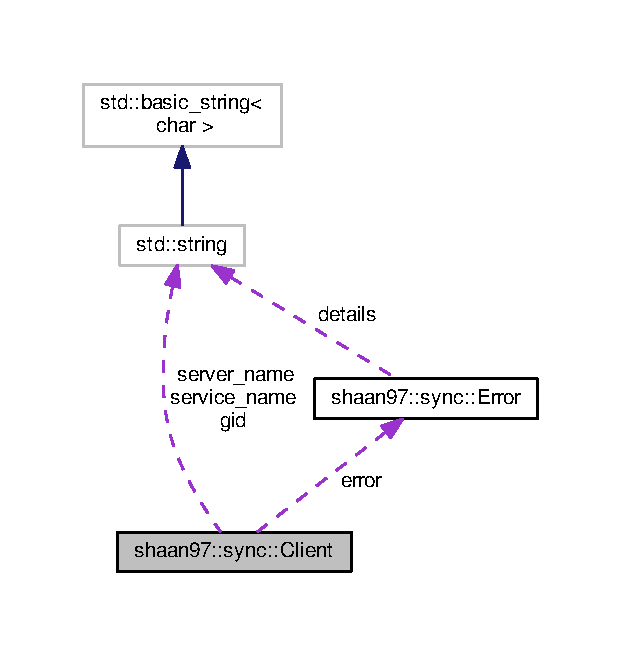
\includegraphics[width=298pt]{classshaan97_1_1sync_1_1_client__coll__graph}
\end{center}
\end{figure}
\subsection*{Public Member Functions}
\begin{DoxyCompactItemize}
\item 
\hyperlink{classshaan97_1_1sync_1_1_client_aa9620e6828907c167babfc66a2926510}{Client} (std\+::string \hyperlink{classshaan97_1_1sync_1_1_client_a8edca95d3206d3c71bf851ad2dea7ec7}{server\+\_\+name}, std\+::string \hyperlink{classshaan97_1_1sync_1_1_client_a80e8c87abf08c599948d6464caa148e7}{service\+\_\+name}=\char`\"{}daytime\char`\"{}, G\+R\+O\+U\+P\+\_\+\+ID \hyperlink{classshaan97_1_1sync_1_1_client_a2708c76151616ac36af4aedecee5beb1}{gid}=\char`\"{}\char`\"{})
\item 
\hyperlink{classshaan97_1_1sync_1_1_client_a89f86d3ee0c7d60930276ff1a49fb203}{Client} (const \hyperlink{classshaan97_1_1sync_1_1_client}{Client} \&c)
\item 
virtual \hyperlink{classshaan97_1_1sync_1_1_client_a840e519ca781888cbd54181572ebe3a7}{$\sim$\+Client} ()
\item 
bool \hyperlink{classshaan97_1_1sync_1_1_client_afa6eb46eb9710b7ee9bbfaec0f70249b}{join\+Group} (\hyperlink{namespaceshaan97_1_1sync_a34cebf175d27dfc3d82f24608f7043c1}{G\+R\+O\+U\+P\+\_\+\+ID} \hyperlink{classshaan97_1_1sync_1_1_client_a2708c76151616ac36af4aedecee5beb1}{gid})
\item 
void \hyperlink{classshaan97_1_1sync_1_1_client_a9822f9f083442f323a8eda5cbe530523}{leave\+Group} ()
\item 
bool \hyperlink{classshaan97_1_1sync_1_1_client_a6afcf79c9a70dc1dee1e357f39343f91}{change\+Group} (\hyperlink{namespaceshaan97_1_1sync_a34cebf175d27dfc3d82f24608f7043c1}{G\+R\+O\+U\+P\+\_\+\+ID} \hyperlink{classshaan97_1_1sync_1_1_client_a2708c76151616ac36af4aedecee5beb1}{gid})
\item 
\hyperlink{namespaceshaan97_1_1sync_a34cebf175d27dfc3d82f24608f7043c1}{G\+R\+O\+U\+P\+\_\+\+ID} \hyperlink{classshaan97_1_1sync_1_1_client_abf8af45f2a8b6bf674357b6fc44fe3cc}{get\+Group} () const
\item 
std\+::pair$<$ \hyperlink{namespaceshaan97_1_1sync_a34cebf175d27dfc3d82f24608f7043c1}{G\+R\+O\+U\+P\+\_\+\+ID}, bool $>$ \hyperlink{classshaan97_1_1sync_1_1_client_a94a60773fd7d212132f44661acac59c7}{make\+Group} (\hyperlink{namespaceshaan97_1_1sync_a34cebf175d27dfc3d82f24608f7043c1}{G\+R\+O\+U\+P\+\_\+\+ID} \hyperlink{classshaan97_1_1sync_1_1_client_a2708c76151616ac36af4aedecee5beb1}{gid}=\char`\"{}\char`\"{})
\item 
bool \hyperlink{classshaan97_1_1sync_1_1_client_a4367779edf080f835087e07b35fa6a38}{is\+Connected} () const
\item 
bool \hyperlink{classshaan97_1_1sync_1_1_client_a603ec6160f76f97fcfb41d099fdea6ab}{propose\+Song} ()
\item 
void \hyperlink{classshaan97_1_1sync_1_1_client_a6429d2c4549c9fd3074f3181923c5906}{swap} (\hyperlink{classshaan97_1_1sync_1_1_client}{Client} \&c)
\item 
\hyperlink{classshaan97_1_1sync_1_1_client}{Client} \& \hyperlink{classshaan97_1_1sync_1_1_client_a807d5ec3cc4cc0bcc3d5dec72fc3af06}{operator=} (const \hyperlink{classshaan97_1_1sync_1_1_client}{Client} \&c)
\end{DoxyCompactItemize}
\subsection*{Private Member Functions}
\begin{DoxyCompactItemize}
\item 
bool \hyperlink{classshaan97_1_1sync_1_1_client_ac3ae19ae773cf3fde376d1d984c10327}{sync\+Group} (std\+::string \hyperlink{classshaan97_1_1sync_1_1_client_a8edca95d3206d3c71bf851ad2dea7ec7}{server\+\_\+name}, std\+::string \hyperlink{classshaan97_1_1sync_1_1_client_a80e8c87abf08c599948d6464caa148e7}{service\+\_\+name}, \hyperlink{namespaceshaan97_1_1sync_a34cebf175d27dfc3d82f24608f7043c1}{G\+R\+O\+U\+P\+\_\+\+ID} \hyperlink{classshaan97_1_1sync_1_1_client_a2708c76151616ac36af4aedecee5beb1}{gid})
\end{DoxyCompactItemize}
\subsection*{Private Attributes}
\begin{DoxyCompactItemize}
\item 
\hyperlink{namespaceshaan97_1_1sync_a34cebf175d27dfc3d82f24608f7043c1}{G\+R\+O\+U\+P\+\_\+\+ID} \hyperlink{classshaan97_1_1sync_1_1_client_a2708c76151616ac36af4aedecee5beb1}{gid}
\item 
bool \hyperlink{classshaan97_1_1sync_1_1_client_a8dc007c6e1c0fb4a20112e8cc10b8b7c}{connected\+To\+Group} = false
\item 
std\+::shared\+\_\+ptr$<$ boost\+::asio\+::io\+\_\+service $>$ \hyperlink{classshaan97_1_1sync_1_1_client_a3012a6e9540155af7245d898bfdd7986}{io\+\_\+service}
\item 
std\+::shared\+\_\+ptr$<$ boost\+::asio\+::ip\+::tcp\+::resolver $>$ \hyperlink{classshaan97_1_1sync_1_1_client_a6e2a1fef479966299280a231815ab6c9}{resolver}
\item 
std\+::shared\+\_\+ptr$<$ boost\+::asio\+::ip\+::tcp\+::resolver\+::query $>$ \hyperlink{classshaan97_1_1sync_1_1_client_a6c37abd3f312836146b4e140b0cf7680}{query}
\item 
std\+::shared\+\_\+ptr$<$ boost\+::asio\+::ip\+::tcp\+::resolver\+::iterator $>$ \hyperlink{classshaan97_1_1sync_1_1_client_a0afe11a920512355f1b23dfff1c42b08}{endpoint\+\_\+iterator}
\item 
std\+::shared\+\_\+ptr$<$ boost\+::asio\+::ip\+::tcp\+::socket $>$ \hyperlink{classshaan97_1_1sync_1_1_client_a55bfc26c9a8e09b61c9075198abd52a6}{socket}
\item 
\hyperlink{classshaan97_1_1sync_1_1_error}{Error} \hyperlink{classshaan97_1_1sync_1_1_client_a302a10619aece387dc9938196740f0c8}{error}
\item 
std\+::string \hyperlink{classshaan97_1_1sync_1_1_client_a8edca95d3206d3c71bf851ad2dea7ec7}{server\+\_\+name}
\item 
std\+::string \hyperlink{classshaan97_1_1sync_1_1_client_a80e8c87abf08c599948d6464caa148e7}{service\+\_\+name}
\end{DoxyCompactItemize}


\subsection{Constructor \& Destructor Documentation}
\mbox{\Hypertarget{classshaan97_1_1sync_1_1_client_aa9620e6828907c167babfc66a2926510}\label{classshaan97_1_1sync_1_1_client_aa9620e6828907c167babfc66a2926510}} 
\index{shaan97\+::sync\+::\+Client@{shaan97\+::sync\+::\+Client}!Client@{Client}}
\index{Client@{Client}!shaan97\+::sync\+::\+Client@{shaan97\+::sync\+::\+Client}}
\subsubsection{\texorpdfstring{Client()}{Client()}\hspace{0.1cm}{\footnotesize\ttfamily [1/2]}}
{\footnotesize\ttfamily Client\+::\+Client (\begin{DoxyParamCaption}\item[{std\+::string}]{server\+\_\+name,  }\item[{std\+::string}]{service\+\_\+name = {\ttfamily \char`\"{}daytime\char`\"{}},  }\item[{\hyperlink{namespaceshaan97_1_1sync_a34cebf175d27dfc3d82f24608f7043c1}{G\+R\+O\+U\+P\+\_\+\+ID}}]{gid = {\ttfamily \char`\"{}\char`\"{}} }\end{DoxyParamCaption})}

Here is the call graph for this function\+:\nopagebreak
\begin{figure}[H]
\begin{center}
\leavevmode
\includegraphics[width=340pt]{classshaan97_1_1sync_1_1_client_aa9620e6828907c167babfc66a2926510_cgraph}
\end{center}
\end{figure}
\mbox{\Hypertarget{classshaan97_1_1sync_1_1_client_a89f86d3ee0c7d60930276ff1a49fb203}\label{classshaan97_1_1sync_1_1_client_a89f86d3ee0c7d60930276ff1a49fb203}} 
\index{shaan97\+::sync\+::\+Client@{shaan97\+::sync\+::\+Client}!Client@{Client}}
\index{Client@{Client}!shaan97\+::sync\+::\+Client@{shaan97\+::sync\+::\+Client}}
\subsubsection{\texorpdfstring{Client()}{Client()}\hspace{0.1cm}{\footnotesize\ttfamily [2/2]}}
{\footnotesize\ttfamily Client\+::\+Client (\begin{DoxyParamCaption}\item[{const \hyperlink{classshaan97_1_1sync_1_1_client}{Client} \&}]{c }\end{DoxyParamCaption})}

\mbox{\Hypertarget{classshaan97_1_1sync_1_1_client_a840e519ca781888cbd54181572ebe3a7}\label{classshaan97_1_1sync_1_1_client_a840e519ca781888cbd54181572ebe3a7}} 
\index{shaan97\+::sync\+::\+Client@{shaan97\+::sync\+::\+Client}!````~Client@{$\sim$\+Client}}
\index{````~Client@{$\sim$\+Client}!shaan97\+::sync\+::\+Client@{shaan97\+::sync\+::\+Client}}
\subsubsection{\texorpdfstring{$\sim$\+Client()}{~Client()}}
{\footnotesize\ttfamily Client\+::$\sim$\+Client (\begin{DoxyParamCaption}{ }\end{DoxyParamCaption})\hspace{0.3cm}{\ttfamily [virtual]}}



\subsection{Member Function Documentation}
\mbox{\Hypertarget{classshaan97_1_1sync_1_1_client_a6afcf79c9a70dc1dee1e357f39343f91}\label{classshaan97_1_1sync_1_1_client_a6afcf79c9a70dc1dee1e357f39343f91}} 
\index{shaan97\+::sync\+::\+Client@{shaan97\+::sync\+::\+Client}!change\+Group@{change\+Group}}
\index{change\+Group@{change\+Group}!shaan97\+::sync\+::\+Client@{shaan97\+::sync\+::\+Client}}
\subsubsection{\texorpdfstring{change\+Group()}{changeGroup()}}
{\footnotesize\ttfamily bool shaan97\+::sync\+::\+Client\+::change\+Group (\begin{DoxyParamCaption}\item[{\hyperlink{namespaceshaan97_1_1sync_a34cebf175d27dfc3d82f24608f7043c1}{G\+R\+O\+U\+P\+\_\+\+ID}}]{gid }\end{DoxyParamCaption})}

\mbox{\Hypertarget{classshaan97_1_1sync_1_1_client_abf8af45f2a8b6bf674357b6fc44fe3cc}\label{classshaan97_1_1sync_1_1_client_abf8af45f2a8b6bf674357b6fc44fe3cc}} 
\index{shaan97\+::sync\+::\+Client@{shaan97\+::sync\+::\+Client}!get\+Group@{get\+Group}}
\index{get\+Group@{get\+Group}!shaan97\+::sync\+::\+Client@{shaan97\+::sync\+::\+Client}}
\subsubsection{\texorpdfstring{get\+Group()}{getGroup()}}
{\footnotesize\ttfamily \hyperlink{namespaceshaan97_1_1sync_a34cebf175d27dfc3d82f24608f7043c1}{G\+R\+O\+U\+P\+\_\+\+ID} shaan97\+::sync\+::\+Client\+::get\+Group (\begin{DoxyParamCaption}{ }\end{DoxyParamCaption}) const\hspace{0.3cm}{\ttfamily [inline]}}

Here is the call graph for this function\+:\nopagebreak
\begin{figure}[H]
\begin{center}
\leavevmode
\includegraphics[width=350pt]{classshaan97_1_1sync_1_1_client_abf8af45f2a8b6bf674357b6fc44fe3cc_cgraph}
\end{center}
\end{figure}
\mbox{\Hypertarget{classshaan97_1_1sync_1_1_client_a4367779edf080f835087e07b35fa6a38}\label{classshaan97_1_1sync_1_1_client_a4367779edf080f835087e07b35fa6a38}} 
\index{shaan97\+::sync\+::\+Client@{shaan97\+::sync\+::\+Client}!is\+Connected@{is\+Connected}}
\index{is\+Connected@{is\+Connected}!shaan97\+::sync\+::\+Client@{shaan97\+::sync\+::\+Client}}
\subsubsection{\texorpdfstring{is\+Connected()}{isConnected()}}
{\footnotesize\ttfamily bool shaan97\+::sync\+::\+Client\+::is\+Connected (\begin{DoxyParamCaption}{ }\end{DoxyParamCaption}) const\hspace{0.3cm}{\ttfamily [inline]}}

Here is the call graph for this function\+:\nopagebreak
\begin{figure}[H]
\begin{center}
\leavevmode
\includegraphics[width=350pt]{classshaan97_1_1sync_1_1_client_a4367779edf080f835087e07b35fa6a38_cgraph}
\end{center}
\end{figure}
\mbox{\Hypertarget{classshaan97_1_1sync_1_1_client_afa6eb46eb9710b7ee9bbfaec0f70249b}\label{classshaan97_1_1sync_1_1_client_afa6eb46eb9710b7ee9bbfaec0f70249b}} 
\index{shaan97\+::sync\+::\+Client@{shaan97\+::sync\+::\+Client}!join\+Group@{join\+Group}}
\index{join\+Group@{join\+Group}!shaan97\+::sync\+::\+Client@{shaan97\+::sync\+::\+Client}}
\subsubsection{\texorpdfstring{join\+Group()}{joinGroup()}}
{\footnotesize\ttfamily bool shaan97\+::sync\+::\+Client\+::join\+Group (\begin{DoxyParamCaption}\item[{\hyperlink{namespaceshaan97_1_1sync_a34cebf175d27dfc3d82f24608f7043c1}{G\+R\+O\+U\+P\+\_\+\+ID}}]{gid }\end{DoxyParamCaption})}

\mbox{\Hypertarget{classshaan97_1_1sync_1_1_client_a9822f9f083442f323a8eda5cbe530523}\label{classshaan97_1_1sync_1_1_client_a9822f9f083442f323a8eda5cbe530523}} 
\index{shaan97\+::sync\+::\+Client@{shaan97\+::sync\+::\+Client}!leave\+Group@{leave\+Group}}
\index{leave\+Group@{leave\+Group}!shaan97\+::sync\+::\+Client@{shaan97\+::sync\+::\+Client}}
\subsubsection{\texorpdfstring{leave\+Group()}{leaveGroup()}}
{\footnotesize\ttfamily void shaan97\+::sync\+::\+Client\+::leave\+Group (\begin{DoxyParamCaption}{ }\end{DoxyParamCaption})}

\mbox{\Hypertarget{classshaan97_1_1sync_1_1_client_a94a60773fd7d212132f44661acac59c7}\label{classshaan97_1_1sync_1_1_client_a94a60773fd7d212132f44661acac59c7}} 
\index{shaan97\+::sync\+::\+Client@{shaan97\+::sync\+::\+Client}!make\+Group@{make\+Group}}
\index{make\+Group@{make\+Group}!shaan97\+::sync\+::\+Client@{shaan97\+::sync\+::\+Client}}
\subsubsection{\texorpdfstring{make\+Group()}{makeGroup()}}
{\footnotesize\ttfamily std\+::pair$<$\hyperlink{namespaceshaan97_1_1sync_a34cebf175d27dfc3d82f24608f7043c1}{G\+R\+O\+U\+P\+\_\+\+ID}, bool$>$ shaan97\+::sync\+::\+Client\+::make\+Group (\begin{DoxyParamCaption}\item[{\hyperlink{namespaceshaan97_1_1sync_a34cebf175d27dfc3d82f24608f7043c1}{G\+R\+O\+U\+P\+\_\+\+ID}}]{gid = {\ttfamily \char`\"{}\char`\"{}} }\end{DoxyParamCaption})}

\mbox{\Hypertarget{classshaan97_1_1sync_1_1_client_a807d5ec3cc4cc0bcc3d5dec72fc3af06}\label{classshaan97_1_1sync_1_1_client_a807d5ec3cc4cc0bcc3d5dec72fc3af06}} 
\index{shaan97\+::sync\+::\+Client@{shaan97\+::sync\+::\+Client}!operator=@{operator=}}
\index{operator=@{operator=}!shaan97\+::sync\+::\+Client@{shaan97\+::sync\+::\+Client}}
\subsubsection{\texorpdfstring{operator=()}{operator=()}}
{\footnotesize\ttfamily \hyperlink{classshaan97_1_1sync_1_1_client}{Client} \& Client\+::operator= (\begin{DoxyParamCaption}\item[{const \hyperlink{classshaan97_1_1sync_1_1_client}{Client} \&}]{c }\end{DoxyParamCaption})}

Here is the call graph for this function\+:\nopagebreak
\begin{figure}[H]
\begin{center}
\leavevmode
\includegraphics[width=340pt]{classshaan97_1_1sync_1_1_client_a807d5ec3cc4cc0bcc3d5dec72fc3af06_cgraph}
\end{center}
\end{figure}
\mbox{\Hypertarget{classshaan97_1_1sync_1_1_client_a603ec6160f76f97fcfb41d099fdea6ab}\label{classshaan97_1_1sync_1_1_client_a603ec6160f76f97fcfb41d099fdea6ab}} 
\index{shaan97\+::sync\+::\+Client@{shaan97\+::sync\+::\+Client}!propose\+Song@{propose\+Song}}
\index{propose\+Song@{propose\+Song}!shaan97\+::sync\+::\+Client@{shaan97\+::sync\+::\+Client}}
\subsubsection{\texorpdfstring{propose\+Song()}{proposeSong()}}
{\footnotesize\ttfamily bool shaan97\+::sync\+::\+Client\+::propose\+Song (\begin{DoxyParamCaption}{ }\end{DoxyParamCaption})}

\mbox{\Hypertarget{classshaan97_1_1sync_1_1_client_a6429d2c4549c9fd3074f3181923c5906}\label{classshaan97_1_1sync_1_1_client_a6429d2c4549c9fd3074f3181923c5906}} 
\index{shaan97\+::sync\+::\+Client@{shaan97\+::sync\+::\+Client}!swap@{swap}}
\index{swap@{swap}!shaan97\+::sync\+::\+Client@{shaan97\+::sync\+::\+Client}}
\subsubsection{\texorpdfstring{swap()}{swap()}}
{\footnotesize\ttfamily void Client\+::swap (\begin{DoxyParamCaption}\item[{\hyperlink{classshaan97_1_1sync_1_1_client}{Client} \&}]{c }\end{DoxyParamCaption})}

\mbox{\Hypertarget{classshaan97_1_1sync_1_1_client_ac3ae19ae773cf3fde376d1d984c10327}\label{classshaan97_1_1sync_1_1_client_ac3ae19ae773cf3fde376d1d984c10327}} 
\index{shaan97\+::sync\+::\+Client@{shaan97\+::sync\+::\+Client}!sync\+Group@{sync\+Group}}
\index{sync\+Group@{sync\+Group}!shaan97\+::sync\+::\+Client@{shaan97\+::sync\+::\+Client}}
\subsubsection{\texorpdfstring{sync\+Group()}{syncGroup()}}
{\footnotesize\ttfamily bool Client\+::sync\+Group (\begin{DoxyParamCaption}\item[{std\+::string}]{server\+\_\+name,  }\item[{std\+::string}]{service\+\_\+name,  }\item[{\hyperlink{namespaceshaan97_1_1sync_a34cebf175d27dfc3d82f24608f7043c1}{G\+R\+O\+U\+P\+\_\+\+ID}}]{gid }\end{DoxyParamCaption})\hspace{0.3cm}{\ttfamily [private]}}



\subsection{Member Data Documentation}
\mbox{\Hypertarget{classshaan97_1_1sync_1_1_client_a8dc007c6e1c0fb4a20112e8cc10b8b7c}\label{classshaan97_1_1sync_1_1_client_a8dc007c6e1c0fb4a20112e8cc10b8b7c}} 
\index{shaan97\+::sync\+::\+Client@{shaan97\+::sync\+::\+Client}!connected\+To\+Group@{connected\+To\+Group}}
\index{connected\+To\+Group@{connected\+To\+Group}!shaan97\+::sync\+::\+Client@{shaan97\+::sync\+::\+Client}}
\subsubsection{\texorpdfstring{connected\+To\+Group}{connectedToGroup}}
{\footnotesize\ttfamily bool shaan97\+::sync\+::\+Client\+::connected\+To\+Group = false\hspace{0.3cm}{\ttfamily [private]}}

\mbox{\Hypertarget{classshaan97_1_1sync_1_1_client_a0afe11a920512355f1b23dfff1c42b08}\label{classshaan97_1_1sync_1_1_client_a0afe11a920512355f1b23dfff1c42b08}} 
\index{shaan97\+::sync\+::\+Client@{shaan97\+::sync\+::\+Client}!endpoint\+\_\+iterator@{endpoint\+\_\+iterator}}
\index{endpoint\+\_\+iterator@{endpoint\+\_\+iterator}!shaan97\+::sync\+::\+Client@{shaan97\+::sync\+::\+Client}}
\subsubsection{\texorpdfstring{endpoint\+\_\+iterator}{endpoint\_iterator}}
{\footnotesize\ttfamily std\+::shared\+\_\+ptr$<$boost\+::asio\+::ip\+::tcp\+::resolver\+::iterator$>$ shaan97\+::sync\+::\+Client\+::endpoint\+\_\+iterator\hspace{0.3cm}{\ttfamily [private]}}

\mbox{\Hypertarget{classshaan97_1_1sync_1_1_client_a302a10619aece387dc9938196740f0c8}\label{classshaan97_1_1sync_1_1_client_a302a10619aece387dc9938196740f0c8}} 
\index{shaan97\+::sync\+::\+Client@{shaan97\+::sync\+::\+Client}!error@{error}}
\index{error@{error}!shaan97\+::sync\+::\+Client@{shaan97\+::sync\+::\+Client}}
\subsubsection{\texorpdfstring{error}{error}}
{\footnotesize\ttfamily \hyperlink{classshaan97_1_1sync_1_1_error}{Error} shaan97\+::sync\+::\+Client\+::error\hspace{0.3cm}{\ttfamily [private]}}

\mbox{\Hypertarget{classshaan97_1_1sync_1_1_client_a2708c76151616ac36af4aedecee5beb1}\label{classshaan97_1_1sync_1_1_client_a2708c76151616ac36af4aedecee5beb1}} 
\index{shaan97\+::sync\+::\+Client@{shaan97\+::sync\+::\+Client}!gid@{gid}}
\index{gid@{gid}!shaan97\+::sync\+::\+Client@{shaan97\+::sync\+::\+Client}}
\subsubsection{\texorpdfstring{gid}{gid}}
{\footnotesize\ttfamily \hyperlink{namespaceshaan97_1_1sync_a34cebf175d27dfc3d82f24608f7043c1}{G\+R\+O\+U\+P\+\_\+\+ID} shaan97\+::sync\+::\+Client\+::gid\hspace{0.3cm}{\ttfamily [private]}}

\mbox{\Hypertarget{classshaan97_1_1sync_1_1_client_a3012a6e9540155af7245d898bfdd7986}\label{classshaan97_1_1sync_1_1_client_a3012a6e9540155af7245d898bfdd7986}} 
\index{shaan97\+::sync\+::\+Client@{shaan97\+::sync\+::\+Client}!io\+\_\+service@{io\+\_\+service}}
\index{io\+\_\+service@{io\+\_\+service}!shaan97\+::sync\+::\+Client@{shaan97\+::sync\+::\+Client}}
\subsubsection{\texorpdfstring{io\+\_\+service}{io\_service}}
{\footnotesize\ttfamily std\+::shared\+\_\+ptr$<$boost\+::asio\+::io\+\_\+service$>$ shaan97\+::sync\+::\+Client\+::io\+\_\+service\hspace{0.3cm}{\ttfamily [private]}}

\mbox{\Hypertarget{classshaan97_1_1sync_1_1_client_a6c37abd3f312836146b4e140b0cf7680}\label{classshaan97_1_1sync_1_1_client_a6c37abd3f312836146b4e140b0cf7680}} 
\index{shaan97\+::sync\+::\+Client@{shaan97\+::sync\+::\+Client}!query@{query}}
\index{query@{query}!shaan97\+::sync\+::\+Client@{shaan97\+::sync\+::\+Client}}
\subsubsection{\texorpdfstring{query}{query}}
{\footnotesize\ttfamily std\+::shared\+\_\+ptr$<$boost\+::asio\+::ip\+::tcp\+::resolver\+::query$>$ shaan97\+::sync\+::\+Client\+::query\hspace{0.3cm}{\ttfamily [private]}}

\mbox{\Hypertarget{classshaan97_1_1sync_1_1_client_a6e2a1fef479966299280a231815ab6c9}\label{classshaan97_1_1sync_1_1_client_a6e2a1fef479966299280a231815ab6c9}} 
\index{shaan97\+::sync\+::\+Client@{shaan97\+::sync\+::\+Client}!resolver@{resolver}}
\index{resolver@{resolver}!shaan97\+::sync\+::\+Client@{shaan97\+::sync\+::\+Client}}
\subsubsection{\texorpdfstring{resolver}{resolver}}
{\footnotesize\ttfamily std\+::shared\+\_\+ptr$<$boost\+::asio\+::ip\+::tcp\+::resolver$>$ shaan97\+::sync\+::\+Client\+::resolver\hspace{0.3cm}{\ttfamily [private]}}

\mbox{\Hypertarget{classshaan97_1_1sync_1_1_client_a8edca95d3206d3c71bf851ad2dea7ec7}\label{classshaan97_1_1sync_1_1_client_a8edca95d3206d3c71bf851ad2dea7ec7}} 
\index{shaan97\+::sync\+::\+Client@{shaan97\+::sync\+::\+Client}!server\+\_\+name@{server\+\_\+name}}
\index{server\+\_\+name@{server\+\_\+name}!shaan97\+::sync\+::\+Client@{shaan97\+::sync\+::\+Client}}
\subsubsection{\texorpdfstring{server\+\_\+name}{server\_name}}
{\footnotesize\ttfamily std\+::string shaan97\+::sync\+::\+Client\+::server\+\_\+name\hspace{0.3cm}{\ttfamily [private]}}

\mbox{\Hypertarget{classshaan97_1_1sync_1_1_client_a80e8c87abf08c599948d6464caa148e7}\label{classshaan97_1_1sync_1_1_client_a80e8c87abf08c599948d6464caa148e7}} 
\index{shaan97\+::sync\+::\+Client@{shaan97\+::sync\+::\+Client}!service\+\_\+name@{service\+\_\+name}}
\index{service\+\_\+name@{service\+\_\+name}!shaan97\+::sync\+::\+Client@{shaan97\+::sync\+::\+Client}}
\subsubsection{\texorpdfstring{service\+\_\+name}{service\_name}}
{\footnotesize\ttfamily std\+::string shaan97\+::sync\+::\+Client\+::service\+\_\+name\hspace{0.3cm}{\ttfamily [private]}}

\mbox{\Hypertarget{classshaan97_1_1sync_1_1_client_a55bfc26c9a8e09b61c9075198abd52a6}\label{classshaan97_1_1sync_1_1_client_a55bfc26c9a8e09b61c9075198abd52a6}} 
\index{shaan97\+::sync\+::\+Client@{shaan97\+::sync\+::\+Client}!socket@{socket}}
\index{socket@{socket}!shaan97\+::sync\+::\+Client@{shaan97\+::sync\+::\+Client}}
\subsubsection{\texorpdfstring{socket}{socket}}
{\footnotesize\ttfamily std\+::shared\+\_\+ptr$<$boost\+::asio\+::ip\+::tcp\+::socket$>$ shaan97\+::sync\+::\+Client\+::socket\hspace{0.3cm}{\ttfamily [private]}}



The documentation for this class was generated from the following files\+:\begin{DoxyCompactItemize}
\item 
/home/shaan/\+Desktop/\+Computer Science/\+Sync/inc/\hyperlink{_client_8h}{Client.\+h}\item 
/home/shaan/\+Desktop/\+Computer Science/\+Sync/src/\hyperlink{_client_8cpp}{Client.\+cpp}\end{DoxyCompactItemize}

\hypertarget{structnlohmann_1_1detail_1_1conjunction}{}\section{nlohmann\+:\+:detail\+:\+:conjunction$<$... $>$ Struct Template Reference}
\label{structnlohmann_1_1detail_1_1conjunction}\index{nlohmann\+::detail\+::conjunction$<$... $>$@{nlohmann\+::detail\+::conjunction$<$... $>$}}


{\ttfamily \#include $<$json.\+hpp$>$}



Inheritance diagram for nlohmann\+:\+:detail\+:\+:conjunction$<$... $>$\+:\nopagebreak
\begin{figure}[H]
\begin{center}
\leavevmode
\includegraphics[width=223pt]{structnlohmann_1_1detail_1_1conjunction__inherit__graph}
\end{center}
\end{figure}


Collaboration diagram for nlohmann\+:\+:detail\+:\+:conjunction$<$... $>$\+:\nopagebreak
\begin{figure}[H]
\begin{center}
\leavevmode
\includegraphics[width=223pt]{structnlohmann_1_1detail_1_1conjunction__coll__graph}
\end{center}
\end{figure}


The documentation for this struct was generated from the following file\+:\begin{DoxyCompactItemize}
\item 
/home/shaan/\+Desktop/\+Computer Science/\+Sync/inc/\hyperlink{json_8hpp}{json.\+hpp}\end{DoxyCompactItemize}

\hypertarget{structnlohmann_1_1detail_1_1conjunction_3_01_b1_01_4}{}\section{nlohmann\+:\+:detail\+:\+:conjunction$<$ B1 $>$ Struct Template Reference}
\label{structnlohmann_1_1detail_1_1conjunction_3_01_b1_01_4}\index{nlohmann\+::detail\+::conjunction$<$ B1 $>$@{nlohmann\+::detail\+::conjunction$<$ B1 $>$}}


{\ttfamily \#include $<$json.\+hpp$>$}



Inheritance diagram for nlohmann\+:\+:detail\+:\+:conjunction$<$ B1 $>$\+:\nopagebreak
\begin{figure}[H]
\begin{center}
\leavevmode
\includegraphics[width=223pt]{structnlohmann_1_1detail_1_1conjunction_3_01_b1_01_4__inherit__graph}
\end{center}
\end{figure}


Collaboration diagram for nlohmann\+:\+:detail\+:\+:conjunction$<$ B1 $>$\+:\nopagebreak
\begin{figure}[H]
\begin{center}
\leavevmode
\includegraphics[width=223pt]{structnlohmann_1_1detail_1_1conjunction_3_01_b1_01_4__coll__graph}
\end{center}
\end{figure}


The documentation for this struct was generated from the following file\+:\begin{DoxyCompactItemize}
\item 
/home/shaan/\+Desktop/\+Computer Science/\+Sync/inc/\hyperlink{json_8hpp}{json.\+hpp}\end{DoxyCompactItemize}

\hypertarget{structnlohmann_1_1detail_1_1conjunction_3_01_b1_00_01_bn_8_8_8_01_4}{}\section{nlohmann\+:\+:detail\+:\+:conjunction$<$ B1, Bn... $>$ Struct Template Reference}
\label{structnlohmann_1_1detail_1_1conjunction_3_01_b1_00_01_bn_8_8_8_01_4}\index{nlohmann\+::detail\+::conjunction$<$ B1, Bn... $>$@{nlohmann\+::detail\+::conjunction$<$ B1, Bn... $>$}}


{\ttfamily \#include $<$json.\+hpp$>$}



Inheritance diagram for nlohmann\+:\+:detail\+:\+:conjunction$<$ B1, Bn... $>$\+:\nopagebreak
\begin{figure}[H]
\begin{center}
\leavevmode
\includegraphics[width=223pt]{structnlohmann_1_1detail_1_1conjunction_3_01_b1_00_01_bn_8_8_8_01_4__inherit__graph}
\end{center}
\end{figure}


Collaboration diagram for nlohmann\+:\+:detail\+:\+:conjunction$<$ B1, Bn... $>$\+:\nopagebreak
\begin{figure}[H]
\begin{center}
\leavevmode
\includegraphics[width=223pt]{structnlohmann_1_1detail_1_1conjunction_3_01_b1_00_01_bn_8_8_8_01_4__coll__graph}
\end{center}
\end{figure}


The documentation for this struct was generated from the following file\+:\begin{DoxyCompactItemize}
\item 
/home/shaan/\+Desktop/\+Computer Science/\+Sync/inc/\hyperlink{json_8hpp}{json.\+hpp}\end{DoxyCompactItemize}

\hypertarget{classshaan97_1_1sync_1_1_error}{}\section{shaan97\+:\+:sync\+:\+:Error Class Reference}
\label{classshaan97_1_1sync_1_1_error}\index{shaan97\+::sync\+::\+Error@{shaan97\+::sync\+::\+Error}}


{\ttfamily \#include $<$Error.\+h$>$}



Collaboration diagram for shaan97\+:\+:sync\+:\+:Error\+:\nopagebreak
\begin{figure}[H]
\begin{center}
\leavevmode
\includegraphics[width=187pt]{classshaan97_1_1sync_1_1_error__coll__graph}
\end{center}
\end{figure}
\subsection*{Public Member Functions}
\begin{DoxyCompactItemize}
\item 
\hyperlink{classshaan97_1_1sync_1_1_error_a8eaff7b62f525d1d33b68438d8ca3b7e}{Error} (const \hyperlink{namespaceshaan97_1_1sync_a69f4d5572314be52626f6a1c8ecc8db9}{E\+R\+R\+O\+R\+\_\+\+T\+Y\+PE} \&e=\hyperlink{namespaceshaan97_1_1sync_a69f4d5572314be52626f6a1c8ecc8db9a52c4a0d7144160a041261253a2a82894}{N\+O\+NE})
\item 
\hyperlink{classshaan97_1_1sync_1_1_error_a23316cc22cfb5377a0d1173ca44066be}{Error} (const boost\+::system\+::error\+\_\+code \&e)
\begin{DoxyCompactList}\small\item\em Constructor initializing via {\ttfamily boost\+::system\+::error\+\_\+code} \end{DoxyCompactList}\item 
\hyperlink{classshaan97_1_1sync_1_1_error_ad98956db1a62bc2269b27e4ba252a598}{Error} (const \hyperlink{namespaceshaan97_1_1sync_a69f4d5572314be52626f6a1c8ecc8db9}{E\+R\+R\+O\+R\+\_\+\+T\+Y\+PE} \&e, const std\+::string \&\hyperlink{classshaan97_1_1sync_1_1_error_a92edb57631c4d7a2f0177f3440111b23}{details})
\item 
\hyperlink{classshaan97_1_1sync_1_1_error_aa8237d2411892451c587189721b7e0c3}{Error} (const boost\+::system\+::error\+\_\+code \&e, const std\+::string \hyperlink{classshaan97_1_1sync_1_1_error_a92edb57631c4d7a2f0177f3440111b23}{details})
\item 
\hyperlink{classshaan97_1_1sync_1_1_error_aef2207b7ee0f2c8105bed5cffda76c68}{Error} (const \hyperlink{classshaan97_1_1sync_1_1_error}{Error} \&\hyperlink{classshaan97_1_1sync_1_1_error_ab84e9af061261009996c1297c5cad5bd}{error})
\begin{DoxyCompactList}\small\item\em Copy constructor. \end{DoxyCompactList}\item 
\hyperlink{classshaan97_1_1sync_1_1_error_a637d6482658ecea21d66ac90e970100b}{Error} (\hyperlink{classshaan97_1_1sync_1_1_error}{Error} \&\&\hyperlink{classshaan97_1_1sync_1_1_error_ab84e9af061261009996c1297c5cad5bd}{error})
\begin{DoxyCompactList}\small\item\em Implement move semantics. \end{DoxyCompactList}\item 
void \hyperlink{classshaan97_1_1sync_1_1_error_abd07d5a3c98e8310160b1c13b1b08049}{set\+Error} (const \hyperlink{namespaceshaan97_1_1sync_a69f4d5572314be52626f6a1c8ecc8db9}{E\+R\+R\+O\+R\+\_\+\+T\+Y\+PE} \&e, const std\+::string \&\hyperlink{classshaan97_1_1sync_1_1_error_a92edb57631c4d7a2f0177f3440111b23}{details}=\char`\"{}\char`\"{})
\item 
void \hyperlink{classshaan97_1_1sync_1_1_error_a6be9dc27fe05da94cdc58fb1e5256e87}{set\+Error} (const boost\+::system\+::error\+\_\+code \&e, const std\+::string \&\hyperlink{classshaan97_1_1sync_1_1_error_a92edb57631c4d7a2f0177f3440111b23}{details}=\char`\"{}\char`\"{})
\item 
std\+::string \hyperlink{classshaan97_1_1sync_1_1_error_a4a805cbe2bd0fb6c3288b7c369f4de61}{get\+Details} () const
\item 
virtual \hyperlink{classshaan97_1_1sync_1_1_error}{Error} \& \hyperlink{classshaan97_1_1sync_1_1_error_aad15762ad2a2e477bcad5e4e0e0f0ca3}{operator=} (\hyperlink{classshaan97_1_1sync_1_1_error}{Error} \&\&\hyperlink{classshaan97_1_1sync_1_1_error_ab84e9af061261009996c1297c5cad5bd}{error})
\begin{DoxyCompactList}\small\item\em Operator= Move Semantics. \end{DoxyCompactList}\item 
void \hyperlink{classshaan97_1_1sync_1_1_error_a84312ccc3b0eecd63945df4b2c7654a0}{swap} (\hyperlink{classshaan97_1_1sync_1_1_error}{Error} \&\hyperlink{classshaan97_1_1sync_1_1_error_ab84e9af061261009996c1297c5cad5bd}{error})
\item 
virtual \hyperlink{classshaan97_1_1sync_1_1_error}{Error} \& \hyperlink{classshaan97_1_1sync_1_1_error_aca9e61b98143dd11af5ddc20e8585641}{operator=} (const \hyperlink{classshaan97_1_1sync_1_1_error}{Error} \&\hyperlink{classshaan97_1_1sync_1_1_error_ab84e9af061261009996c1297c5cad5bd}{error})
\item 
bool \hyperlink{group___syntactic_sugar_ga54d9f727bc1777cb9485765b070f0f97}{operator==} (const \hyperlink{classshaan97_1_1sync_1_1_error}{Error} \&e)
\item 
bool \hyperlink{group___syntactic_sugar_gaece1c258e0e4bcfba00769313c8370ad}{operator==} (const \hyperlink{namespaceshaan97_1_1sync_a69f4d5572314be52626f6a1c8ecc8db9}{E\+R\+R\+O\+R\+\_\+\+T\+Y\+PE} \&e)
\item 
bool \hyperlink{group___syntactic_sugar_ga46d610d78d061c030e562563f947e196}{operator==} (const boost\+::system\+::error\+\_\+code \&e)
\item 
bool \hyperlink{group___syntactic_sugar_ga43ee206eb49d8427e6c85ed7a4e2f62d}{operator!=} (const \hyperlink{classshaan97_1_1sync_1_1_error}{Error} \&e)
\item 
bool \hyperlink{group___syntactic_sugar_ga93d2c3b440e64d2c2e5385989af96d16}{operator!=} (const \hyperlink{namespaceshaan97_1_1sync_a69f4d5572314be52626f6a1c8ecc8db9}{E\+R\+R\+O\+R\+\_\+\+T\+Y\+PE} \&e)
\item 
bool \hyperlink{group___syntactic_sugar_ga67831fc5e4cef9661a5158acdb33da25}{operator!=} (const boost\+::system\+::error\+\_\+code \&e)
\item 
\hyperlink{group___syntactic_sugar_gaba6a2a8da1a2771f4a007020eb27b256}{operator bool} () const
\begin{DoxyCompactList}\small\item\em True if there was an error. \end{DoxyCompactList}\end{DoxyCompactItemize}
\subsection*{Private Attributes}
\begin{DoxyCompactItemize}
\item 
\hyperlink{namespaceshaan97_1_1sync_a69f4d5572314be52626f6a1c8ecc8db9}{E\+R\+R\+O\+R\+\_\+\+T\+Y\+PE} \hyperlink{classshaan97_1_1sync_1_1_error_ab84e9af061261009996c1297c5cad5bd}{error}
\begin{DoxyCompactList}\small\item\em Type of error. \end{DoxyCompactList}\item 
std\+::string \hyperlink{classshaan97_1_1sync_1_1_error_a92edb57631c4d7a2f0177f3440111b23}{details}
\begin{DoxyCompactList}\small\item\em Details of the error (may be empty) \end{DoxyCompactList}\item 
boost\+::system\+::error\+\_\+code \hyperlink{classshaan97_1_1sync_1_1_error_ac5664dc7101fda44de7145dbf17a0923}{boost\+\_\+error}
\item 
bool \hyperlink{classshaan97_1_1sync_1_1_error_afc11f4b04e46329a1317d157d4d92771}{is\+Boost\+Error}
\end{DoxyCompactItemize}
\subsection*{Friends}
\begin{DoxyCompactItemize}
\item 
std\+::ostream \& \hyperlink{group___syntactic_sugar_ga988539f900b9f29d5444b633f0857347}{operator$<$$<$} (std\+::ostream \&out, const \hyperlink{classshaan97_1_1sync_1_1_error}{Error} \&e)
\begin{DoxyCompactList}\small\item\em Can be used to send formatted string to ostream. \end{DoxyCompactList}\item 
void \hyperlink{group___serialization_ga06e5a619d8d673a3bb00b006e62bbe1e}{to\+\_\+json} (\hyperlink{namespacenlohmann_a2bfd99e845a2e5cd90aeaf1b1431f474}{nlohmann\+::json} \&j, const \hyperlink{classshaan97_1_1sync_1_1_error}{Error} \&e)
\item 
void \hyperlink{group___serialization_ga827d73b9e95e7aa59bf1b159251bedf3}{from\+\_\+json} (\hyperlink{namespacenlohmann_a2bfd99e845a2e5cd90aeaf1b1431f474}{nlohmann\+::json} \&j, \hyperlink{classshaan97_1_1sync_1_1_error}{Error} \&e)
\end{DoxyCompactItemize}


\subsection{Constructor \& Destructor Documentation}
\mbox{\Hypertarget{classshaan97_1_1sync_1_1_error_a8eaff7b62f525d1d33b68438d8ca3b7e}\label{classshaan97_1_1sync_1_1_error_a8eaff7b62f525d1d33b68438d8ca3b7e}} 
\index{shaan97\+::sync\+::\+Error@{shaan97\+::sync\+::\+Error}!Error@{Error}}
\index{Error@{Error}!shaan97\+::sync\+::\+Error@{shaan97\+::sync\+::\+Error}}
\subsubsection{\texorpdfstring{Error()}{Error()}\hspace{0.1cm}{\footnotesize\ttfamily [1/6]}}
{\footnotesize\ttfamily Error\+::\+Error (\begin{DoxyParamCaption}\item[{const \hyperlink{namespaceshaan97_1_1sync_a69f4d5572314be52626f6a1c8ecc8db9}{E\+R\+R\+O\+R\+\_\+\+T\+Y\+PE} \&}]{e = {\ttfamily \hyperlink{namespaceshaan97_1_1sync_a69f4d5572314be52626f6a1c8ecc8db9a52c4a0d7144160a041261253a2a82894}{N\+O\+NE}} }\end{DoxyParamCaption})}

Constructor initializing via {\ttfamily E\+R\+R\+O\+R\+\_\+\+T\+Y\+PE} \begin{DoxyNote}{Note}
There is convenience with implicit type casting for E\+R\+R\+O\+R\+\_\+\+T\+Y\+PE 
\end{DoxyNote}
Here is the call graph for this function\+:\nopagebreak
\begin{figure}[H]
\begin{center}
\leavevmode
\includegraphics[width=296pt]{classshaan97_1_1sync_1_1_error_a8eaff7b62f525d1d33b68438d8ca3b7e_cgraph}
\end{center}
\end{figure}
\mbox{\Hypertarget{classshaan97_1_1sync_1_1_error_a23316cc22cfb5377a0d1173ca44066be}\label{classshaan97_1_1sync_1_1_error_a23316cc22cfb5377a0d1173ca44066be}} 
\index{shaan97\+::sync\+::\+Error@{shaan97\+::sync\+::\+Error}!Error@{Error}}
\index{Error@{Error}!shaan97\+::sync\+::\+Error@{shaan97\+::sync\+::\+Error}}
\subsubsection{\texorpdfstring{Error()}{Error()}\hspace{0.1cm}{\footnotesize\ttfamily [2/6]}}
{\footnotesize\ttfamily Error\+::\+Error (\begin{DoxyParamCaption}\item[{const boost\+::system\+::error\+\_\+code \&}]{e }\end{DoxyParamCaption})}



Constructor initializing via {\ttfamily boost\+::system\+::error\+\_\+code} 

\mbox{\Hypertarget{classshaan97_1_1sync_1_1_error_ad98956db1a62bc2269b27e4ba252a598}\label{classshaan97_1_1sync_1_1_error_ad98956db1a62bc2269b27e4ba252a598}} 
\index{shaan97\+::sync\+::\+Error@{shaan97\+::sync\+::\+Error}!Error@{Error}}
\index{Error@{Error}!shaan97\+::sync\+::\+Error@{shaan97\+::sync\+::\+Error}}
\subsubsection{\texorpdfstring{Error()}{Error()}\hspace{0.1cm}{\footnotesize\ttfamily [3/6]}}
{\footnotesize\ttfamily Error\+::\+Error (\begin{DoxyParamCaption}\item[{const \hyperlink{namespaceshaan97_1_1sync_a69f4d5572314be52626f6a1c8ecc8db9}{E\+R\+R\+O\+R\+\_\+\+T\+Y\+PE} \&}]{e,  }\item[{const std\+::string \&}]{details }\end{DoxyParamCaption})}

Constructors with the additional option of adding details about the error 
\begin{DoxyParams}{Parameters}
{\em e} & The type of error \\
\hline
{\em details} & Case specific info on the error \\
\hline
\end{DoxyParams}
Here is the call graph for this function\+:\nopagebreak
\begin{figure}[H]
\begin{center}
\leavevmode
\includegraphics[width=296pt]{classshaan97_1_1sync_1_1_error_ad98956db1a62bc2269b27e4ba252a598_cgraph}
\end{center}
\end{figure}
\mbox{\Hypertarget{classshaan97_1_1sync_1_1_error_aa8237d2411892451c587189721b7e0c3}\label{classshaan97_1_1sync_1_1_error_aa8237d2411892451c587189721b7e0c3}} 
\index{shaan97\+::sync\+::\+Error@{shaan97\+::sync\+::\+Error}!Error@{Error}}
\index{Error@{Error}!shaan97\+::sync\+::\+Error@{shaan97\+::sync\+::\+Error}}
\subsubsection{\texorpdfstring{Error()}{Error()}\hspace{0.1cm}{\footnotesize\ttfamily [4/6]}}
{\footnotesize\ttfamily Error\+::\+Error (\begin{DoxyParamCaption}\item[{const boost\+::system\+::error\+\_\+code \&}]{e,  }\item[{const std\+::string}]{details }\end{DoxyParamCaption})}

\mbox{\Hypertarget{classshaan97_1_1sync_1_1_error_aef2207b7ee0f2c8105bed5cffda76c68}\label{classshaan97_1_1sync_1_1_error_aef2207b7ee0f2c8105bed5cffda76c68}} 
\index{shaan97\+::sync\+::\+Error@{shaan97\+::sync\+::\+Error}!Error@{Error}}
\index{Error@{Error}!shaan97\+::sync\+::\+Error@{shaan97\+::sync\+::\+Error}}
\subsubsection{\texorpdfstring{Error()}{Error()}\hspace{0.1cm}{\footnotesize\ttfamily [5/6]}}
{\footnotesize\ttfamily Error\+::\+Error (\begin{DoxyParamCaption}\item[{const \hyperlink{classshaan97_1_1sync_1_1_error}{Error} \&}]{error }\end{DoxyParamCaption})}



Copy constructor. 

\mbox{\Hypertarget{classshaan97_1_1sync_1_1_error_a637d6482658ecea21d66ac90e970100b}\label{classshaan97_1_1sync_1_1_error_a637d6482658ecea21d66ac90e970100b}} 
\index{shaan97\+::sync\+::\+Error@{shaan97\+::sync\+::\+Error}!Error@{Error}}
\index{Error@{Error}!shaan97\+::sync\+::\+Error@{shaan97\+::sync\+::\+Error}}
\subsubsection{\texorpdfstring{Error()}{Error()}\hspace{0.1cm}{\footnotesize\ttfamily [6/6]}}
{\footnotesize\ttfamily Error\+::\+Error (\begin{DoxyParamCaption}\item[{\hyperlink{classshaan97_1_1sync_1_1_error}{Error} \&\&}]{error }\end{DoxyParamCaption})}



Implement move semantics. 



\subsection{Member Function Documentation}
\mbox{\Hypertarget{classshaan97_1_1sync_1_1_error_a4a805cbe2bd0fb6c3288b7c369f4de61}\label{classshaan97_1_1sync_1_1_error_a4a805cbe2bd0fb6c3288b7c369f4de61}} 
\index{shaan97\+::sync\+::\+Error@{shaan97\+::sync\+::\+Error}!get\+Details@{get\+Details}}
\index{get\+Details@{get\+Details}!shaan97\+::sync\+::\+Error@{shaan97\+::sync\+::\+Error}}
\subsubsection{\texorpdfstring{get\+Details()}{getDetails()}}
{\footnotesize\ttfamily std\+::string Error\+::get\+Details (\begin{DoxyParamCaption}{ }\end{DoxyParamCaption}) const}

\begin{DoxyReturn}{Returns}
Produces formatted string detailing the type of error and potentially a message 
\end{DoxyReturn}
\mbox{\Hypertarget{classshaan97_1_1sync_1_1_error_aad15762ad2a2e477bcad5e4e0e0f0ca3}\label{classshaan97_1_1sync_1_1_error_aad15762ad2a2e477bcad5e4e0e0f0ca3}} 
\index{shaan97\+::sync\+::\+Error@{shaan97\+::sync\+::\+Error}!operator=@{operator=}}
\index{operator=@{operator=}!shaan97\+::sync\+::\+Error@{shaan97\+::sync\+::\+Error}}
\subsubsection{\texorpdfstring{operator=()}{operator=()}\hspace{0.1cm}{\footnotesize\ttfamily [1/2]}}
{\footnotesize\ttfamily \hyperlink{classshaan97_1_1sync_1_1_error}{Error} \& Error\+::operator= (\begin{DoxyParamCaption}\item[{\hyperlink{classshaan97_1_1sync_1_1_error}{Error} \&\&}]{error }\end{DoxyParamCaption})\hspace{0.3cm}{\ttfamily [virtual]}}



Operator= Move Semantics. 

\mbox{\Hypertarget{classshaan97_1_1sync_1_1_error_aca9e61b98143dd11af5ddc20e8585641}\label{classshaan97_1_1sync_1_1_error_aca9e61b98143dd11af5ddc20e8585641}} 
\index{shaan97\+::sync\+::\+Error@{shaan97\+::sync\+::\+Error}!operator=@{operator=}}
\index{operator=@{operator=}!shaan97\+::sync\+::\+Error@{shaan97\+::sync\+::\+Error}}
\subsubsection{\texorpdfstring{operator=()}{operator=()}\hspace{0.1cm}{\footnotesize\ttfamily [2/2]}}
{\footnotesize\ttfamily \hyperlink{classshaan97_1_1sync_1_1_error}{Error} \& Error\+::operator= (\begin{DoxyParamCaption}\item[{const \hyperlink{classshaan97_1_1sync_1_1_error}{Error} \&}]{error }\end{DoxyParamCaption})\hspace{0.3cm}{\ttfamily [virtual]}}

Here is the call graph for this function\+:\nopagebreak
\begin{figure}[H]
\begin{center}
\leavevmode
\includegraphics[width=330pt]{classshaan97_1_1sync_1_1_error_aca9e61b98143dd11af5ddc20e8585641_cgraph}
\end{center}
\end{figure}
\mbox{\Hypertarget{classshaan97_1_1sync_1_1_error_abd07d5a3c98e8310160b1c13b1b08049}\label{classshaan97_1_1sync_1_1_error_abd07d5a3c98e8310160b1c13b1b08049}} 
\index{shaan97\+::sync\+::\+Error@{shaan97\+::sync\+::\+Error}!set\+Error@{set\+Error}}
\index{set\+Error@{set\+Error}!shaan97\+::sync\+::\+Error@{shaan97\+::sync\+::\+Error}}
\subsubsection{\texorpdfstring{set\+Error()}{setError()}\hspace{0.1cm}{\footnotesize\ttfamily [1/2]}}
{\footnotesize\ttfamily void Error\+::set\+Error (\begin{DoxyParamCaption}\item[{const \hyperlink{namespaceshaan97_1_1sync_a69f4d5572314be52626f6a1c8ecc8db9}{E\+R\+R\+O\+R\+\_\+\+T\+Y\+PE} \&}]{e,  }\item[{const std\+::string \&}]{details = {\ttfamily \char`\"{}\char`\"{}} }\end{DoxyParamCaption})}

Mutator for {\ttfamily E\+R\+R\+O\+R\+\_\+\+T\+Y\+PE} \begin{DoxyNote}{Note}
If switching between E\+R\+R\+O\+R\+\_\+\+T\+Y\+PE and boost\+::system\+::error\+\_\+code then the old value is invalidated. 
\end{DoxyNote}
Here is the call graph for this function\+:\nopagebreak
\begin{figure}[H]
\begin{center}
\leavevmode
\includegraphics[width=296pt]{classshaan97_1_1sync_1_1_error_abd07d5a3c98e8310160b1c13b1b08049_cgraph}
\end{center}
\end{figure}
\mbox{\Hypertarget{classshaan97_1_1sync_1_1_error_a6be9dc27fe05da94cdc58fb1e5256e87}\label{classshaan97_1_1sync_1_1_error_a6be9dc27fe05da94cdc58fb1e5256e87}} 
\index{shaan97\+::sync\+::\+Error@{shaan97\+::sync\+::\+Error}!set\+Error@{set\+Error}}
\index{set\+Error@{set\+Error}!shaan97\+::sync\+::\+Error@{shaan97\+::sync\+::\+Error}}
\subsubsection{\texorpdfstring{set\+Error()}{setError()}\hspace{0.1cm}{\footnotesize\ttfamily [2/2]}}
{\footnotesize\ttfamily void Error\+::set\+Error (\begin{DoxyParamCaption}\item[{const boost\+::system\+::error\+\_\+code \&}]{e,  }\item[{const std\+::string \&}]{details = {\ttfamily \char`\"{}\char`\"{}} }\end{DoxyParamCaption})}

Mutator for {\ttfamily boost\+::system\+::error\+\_\+code} \begin{DoxyNote}{Note}
If switching between E\+R\+R\+O\+R\+\_\+\+T\+Y\+PE and boost\+::system\+::error\+\_\+code then the old value is invalidated. 
\end{DoxyNote}
\mbox{\Hypertarget{classshaan97_1_1sync_1_1_error_a84312ccc3b0eecd63945df4b2c7654a0}\label{classshaan97_1_1sync_1_1_error_a84312ccc3b0eecd63945df4b2c7654a0}} 
\index{shaan97\+::sync\+::\+Error@{shaan97\+::sync\+::\+Error}!swap@{swap}}
\index{swap@{swap}!shaan97\+::sync\+::\+Error@{shaan97\+::sync\+::\+Error}}
\subsubsection{\texorpdfstring{swap()}{swap()}}
{\footnotesize\ttfamily void Error\+::swap (\begin{DoxyParamCaption}\item[{\hyperlink{classshaan97_1_1sync_1_1_error}{Error} \&}]{error }\end{DoxyParamCaption})}



\subsection{Member Data Documentation}
\mbox{\Hypertarget{classshaan97_1_1sync_1_1_error_ac5664dc7101fda44de7145dbf17a0923}\label{classshaan97_1_1sync_1_1_error_ac5664dc7101fda44de7145dbf17a0923}} 
\index{shaan97\+::sync\+::\+Error@{shaan97\+::sync\+::\+Error}!boost\+\_\+error@{boost\+\_\+error}}
\index{boost\+\_\+error@{boost\+\_\+error}!shaan97\+::sync\+::\+Error@{shaan97\+::sync\+::\+Error}}
\subsubsection{\texorpdfstring{boost\+\_\+error}{boost\_error}}
{\footnotesize\ttfamily boost\+::system\+::error\+\_\+code shaan97\+::sync\+::\+Error\+::boost\+\_\+error\hspace{0.3cm}{\ttfamily [private]}}

\mbox{\Hypertarget{classshaan97_1_1sync_1_1_error_a92edb57631c4d7a2f0177f3440111b23}\label{classshaan97_1_1sync_1_1_error_a92edb57631c4d7a2f0177f3440111b23}} 
\index{shaan97\+::sync\+::\+Error@{shaan97\+::sync\+::\+Error}!details@{details}}
\index{details@{details}!shaan97\+::sync\+::\+Error@{shaan97\+::sync\+::\+Error}}
\subsubsection{\texorpdfstring{details}{details}}
{\footnotesize\ttfamily std\+::string shaan97\+::sync\+::\+Error\+::details\hspace{0.3cm}{\ttfamily [private]}}



Details of the error (may be empty) 

\mbox{\Hypertarget{classshaan97_1_1sync_1_1_error_ab84e9af061261009996c1297c5cad5bd}\label{classshaan97_1_1sync_1_1_error_ab84e9af061261009996c1297c5cad5bd}} 
\index{shaan97\+::sync\+::\+Error@{shaan97\+::sync\+::\+Error}!error@{error}}
\index{error@{error}!shaan97\+::sync\+::\+Error@{shaan97\+::sync\+::\+Error}}
\subsubsection{\texorpdfstring{error}{error}}
{\footnotesize\ttfamily \hyperlink{namespaceshaan97_1_1sync_a69f4d5572314be52626f6a1c8ecc8db9}{E\+R\+R\+O\+R\+\_\+\+T\+Y\+PE} shaan97\+::sync\+::\+Error\+::error\hspace{0.3cm}{\ttfamily [private]}}



Type of error. 

\mbox{\Hypertarget{classshaan97_1_1sync_1_1_error_afc11f4b04e46329a1317d157d4d92771}\label{classshaan97_1_1sync_1_1_error_afc11f4b04e46329a1317d157d4d92771}} 
\index{shaan97\+::sync\+::\+Error@{shaan97\+::sync\+::\+Error}!is\+Boost\+Error@{is\+Boost\+Error}}
\index{is\+Boost\+Error@{is\+Boost\+Error}!shaan97\+::sync\+::\+Error@{shaan97\+::sync\+::\+Error}}
\subsubsection{\texorpdfstring{is\+Boost\+Error}{isBoostError}}
{\footnotesize\ttfamily bool shaan97\+::sync\+::\+Error\+::is\+Boost\+Error\hspace{0.3cm}{\ttfamily [private]}}



The documentation for this class was generated from the following files\+:\begin{DoxyCompactItemize}
\item 
/home/shaan/\+Desktop/\+Computer Science/\+Sync/inc/\hyperlink{_error_8h}{Error.\+h}\item 
/home/shaan/\+Desktop/\+Computer Science/\+Sync/src/\hyperlink{_error_8cpp}{Error.\+cpp}\end{DoxyCompactItemize}

\hypertarget{structnlohmann_1_1detail_1_1external__constructor}{}\section{nlohmann\+:\+:detail\+:\+:external\+\_\+constructor$<$ value\+\_\+t $>$ Struct Template Reference}
\label{structnlohmann_1_1detail_1_1external__constructor}\index{nlohmann\+::detail\+::external\+\_\+constructor$<$ value\+\_\+t $>$@{nlohmann\+::detail\+::external\+\_\+constructor$<$ value\+\_\+t $>$}}


{\ttfamily \#include $<$json.\+hpp$>$}



The documentation for this struct was generated from the following file\+:\begin{DoxyCompactItemize}
\item 
/home/shaan/\+Desktop/\+Computer Science/\+Sync/inc/\hyperlink{json_8hpp}{json.\+hpp}\end{DoxyCompactItemize}

\hypertarget{structnlohmann_1_1detail_1_1external__constructor_3_01value__t_1_1array_01_4}{}\section{nlohmann\+:\+:detail\+:\+:external\+\_\+constructor$<$ value\+\_\+t\+:\+:array $>$ Struct Template Reference}
\label{structnlohmann_1_1detail_1_1external__constructor_3_01value__t_1_1array_01_4}\index{nlohmann\+::detail\+::external\+\_\+constructor$<$ value\+\_\+t\+::array $>$@{nlohmann\+::detail\+::external\+\_\+constructor$<$ value\+\_\+t\+::array $>$}}


{\ttfamily \#include $<$json.\+hpp$>$}

\subsection*{Static Public Member Functions}
\begin{DoxyCompactItemize}
\item 
{\footnotesize template$<$typename Basic\+Json\+Type $>$ }\\static void \hyperlink{structnlohmann_1_1detail_1_1external__constructor_3_01value__t_1_1array_01_4_abfb2a6eec0bc21e8a7438546aebc55d8}{construct} (Basic\+Json\+Type \&j, const typename Basic\+Json\+Type\+::array\+\_\+t \&arr)
\item 
{\footnotesize template$<$typename Basic\+Json\+Type , typename Compatible\+Array\+Type , enable\+\_\+if\+\_\+t$<$ not std\+::is\+\_\+same$<$ Compatible\+Array\+Type, typename Basic\+Json\+Type\+::array\+\_\+t $>$\+::value, int $>$  = 0$>$ }\\static void \hyperlink{structnlohmann_1_1detail_1_1external__constructor_3_01value__t_1_1array_01_4_a110f50fd5378da876d9a6d6a8d945e37}{construct} (Basic\+Json\+Type \&j, const Compatible\+Array\+Type \&arr)
\end{DoxyCompactItemize}


\subsection{Member Function Documentation}
\mbox{\Hypertarget{structnlohmann_1_1detail_1_1external__constructor_3_01value__t_1_1array_01_4_abfb2a6eec0bc21e8a7438546aebc55d8}\label{structnlohmann_1_1detail_1_1external__constructor_3_01value__t_1_1array_01_4_abfb2a6eec0bc21e8a7438546aebc55d8}} 
\index{nlohmann\+::detail\+::external\+\_\+constructor$<$ value\+\_\+t\+::array $>$@{nlohmann\+::detail\+::external\+\_\+constructor$<$ value\+\_\+t\+::array $>$}!construct@{construct}}
\index{construct@{construct}!nlohmann\+::detail\+::external\+\_\+constructor$<$ value\+\_\+t\+::array $>$@{nlohmann\+::detail\+::external\+\_\+constructor$<$ value\+\_\+t\+::array $>$}}
\subsubsection{\texorpdfstring{construct()}{construct()}\hspace{0.1cm}{\footnotesize\ttfamily [1/2]}}
{\footnotesize\ttfamily template$<$typename Basic\+Json\+Type $>$ \\
static void \hyperlink{structnlohmann_1_1detail_1_1external__constructor}{nlohmann\+::detail\+::external\+\_\+constructor}$<$ \hyperlink{namespacenlohmann_1_1detail_a90aa5ef615aa8305e9ea20d8a947980faf1f713c9e000f5d3f280adbd124df4f5}{value\+\_\+t\+::array} $>$\+::construct (\begin{DoxyParamCaption}\item[{Basic\+Json\+Type \&}]{j,  }\item[{const typename Basic\+Json\+Type\+::array\+\_\+t \&}]{arr }\end{DoxyParamCaption})\hspace{0.3cm}{\ttfamily [inline]}, {\ttfamily [static]}}

\mbox{\Hypertarget{structnlohmann_1_1detail_1_1external__constructor_3_01value__t_1_1array_01_4_a110f50fd5378da876d9a6d6a8d945e37}\label{structnlohmann_1_1detail_1_1external__constructor_3_01value__t_1_1array_01_4_a110f50fd5378da876d9a6d6a8d945e37}} 
\index{nlohmann\+::detail\+::external\+\_\+constructor$<$ value\+\_\+t\+::array $>$@{nlohmann\+::detail\+::external\+\_\+constructor$<$ value\+\_\+t\+::array $>$}!construct@{construct}}
\index{construct@{construct}!nlohmann\+::detail\+::external\+\_\+constructor$<$ value\+\_\+t\+::array $>$@{nlohmann\+::detail\+::external\+\_\+constructor$<$ value\+\_\+t\+::array $>$}}
\subsubsection{\texorpdfstring{construct()}{construct()}\hspace{0.1cm}{\footnotesize\ttfamily [2/2]}}
{\footnotesize\ttfamily template$<$typename Basic\+Json\+Type , typename Compatible\+Array\+Type , enable\+\_\+if\+\_\+t$<$ not std\+::is\+\_\+same$<$ Compatible\+Array\+Type, typename Basic\+Json\+Type\+::array\+\_\+t $>$\+::value, int $>$  = 0$>$ \\
static void \hyperlink{structnlohmann_1_1detail_1_1external__constructor}{nlohmann\+::detail\+::external\+\_\+constructor}$<$ \hyperlink{namespacenlohmann_1_1detail_a90aa5ef615aa8305e9ea20d8a947980faf1f713c9e000f5d3f280adbd124df4f5}{value\+\_\+t\+::array} $>$\+::construct (\begin{DoxyParamCaption}\item[{Basic\+Json\+Type \&}]{j,  }\item[{const Compatible\+Array\+Type \&}]{arr }\end{DoxyParamCaption})\hspace{0.3cm}{\ttfamily [inline]}, {\ttfamily [static]}}



The documentation for this struct was generated from the following file\+:\begin{DoxyCompactItemize}
\item 
/home/shaan/\+Desktop/\+Computer Science/\+Sync/inc/\hyperlink{json_8hpp}{json.\+hpp}\end{DoxyCompactItemize}

\hypertarget{structnlohmann_1_1detail_1_1external__constructor_3_01value__t_1_1boolean_01_4}{}\section{nlohmann\+:\+:detail\+:\+:external\+\_\+constructor$<$ value\+\_\+t\+:\+:boolean $>$ Struct Template Reference}
\label{structnlohmann_1_1detail_1_1external__constructor_3_01value__t_1_1boolean_01_4}\index{nlohmann\+::detail\+::external\+\_\+constructor$<$ value\+\_\+t\+::boolean $>$@{nlohmann\+::detail\+::external\+\_\+constructor$<$ value\+\_\+t\+::boolean $>$}}


{\ttfamily \#include $<$json.\+hpp$>$}

\subsection*{Static Public Member Functions}
\begin{DoxyCompactItemize}
\item 
{\footnotesize template$<$typename Basic\+Json\+Type $>$ }\\static void \hyperlink{structnlohmann_1_1detail_1_1external__constructor_3_01value__t_1_1boolean_01_4_a867122bcf0856c757bd6bcbfb8be74bc}{construct} (Basic\+Json\+Type \&j, typename Basic\+Json\+Type\+::boolean\+\_\+t b) noexcept
\end{DoxyCompactItemize}


\subsection{Member Function Documentation}
\mbox{\Hypertarget{structnlohmann_1_1detail_1_1external__constructor_3_01value__t_1_1boolean_01_4_a867122bcf0856c757bd6bcbfb8be74bc}\label{structnlohmann_1_1detail_1_1external__constructor_3_01value__t_1_1boolean_01_4_a867122bcf0856c757bd6bcbfb8be74bc}} 
\index{nlohmann\+::detail\+::external\+\_\+constructor$<$ value\+\_\+t\+::boolean $>$@{nlohmann\+::detail\+::external\+\_\+constructor$<$ value\+\_\+t\+::boolean $>$}!construct@{construct}}
\index{construct@{construct}!nlohmann\+::detail\+::external\+\_\+constructor$<$ value\+\_\+t\+::boolean $>$@{nlohmann\+::detail\+::external\+\_\+constructor$<$ value\+\_\+t\+::boolean $>$}}
\subsubsection{\texorpdfstring{construct()}{construct()}}
{\footnotesize\ttfamily template$<$typename Basic\+Json\+Type $>$ \\
static void \hyperlink{structnlohmann_1_1detail_1_1external__constructor}{nlohmann\+::detail\+::external\+\_\+constructor}$<$ \hyperlink{namespacenlohmann_1_1detail_a90aa5ef615aa8305e9ea20d8a947980fa84e2c64f38f78ba3ea5c905ab5a2da27}{value\+\_\+t\+::boolean} $>$\+::construct (\begin{DoxyParamCaption}\item[{Basic\+Json\+Type \&}]{j,  }\item[{typename Basic\+Json\+Type\+::boolean\+\_\+t}]{b }\end{DoxyParamCaption})\hspace{0.3cm}{\ttfamily [inline]}, {\ttfamily [static]}, {\ttfamily [noexcept]}}



The documentation for this struct was generated from the following file\+:\begin{DoxyCompactItemize}
\item 
/home/shaan/\+Desktop/\+Computer Science/\+Sync/inc/\hyperlink{json_8hpp}{json.\+hpp}\end{DoxyCompactItemize}

\hypertarget{structnlohmann_1_1detail_1_1external__constructor_3_01value__t_1_1number__float_01_4}{}\section{nlohmann\+:\+:detail\+:\+:external\+\_\+constructor$<$ value\+\_\+t\+:\+:number\+\_\+float $>$ Struct Template Reference}
\label{structnlohmann_1_1detail_1_1external__constructor_3_01value__t_1_1number__float_01_4}\index{nlohmann\+::detail\+::external\+\_\+constructor$<$ value\+\_\+t\+::number\+\_\+float $>$@{nlohmann\+::detail\+::external\+\_\+constructor$<$ value\+\_\+t\+::number\+\_\+float $>$}}


{\ttfamily \#include $<$json.\+hpp$>$}

\subsection*{Static Public Member Functions}
\begin{DoxyCompactItemize}
\item 
{\footnotesize template$<$typename Basic\+Json\+Type $>$ }\\static void \hyperlink{structnlohmann_1_1detail_1_1external__constructor_3_01value__t_1_1number__float_01_4_a669df5a4d258b588e67f747c6d656cdb}{construct} (Basic\+Json\+Type \&j, typename Basic\+Json\+Type\+::number\+\_\+float\+\_\+t val) noexcept
\end{DoxyCompactItemize}


\subsection{Member Function Documentation}
\mbox{\Hypertarget{structnlohmann_1_1detail_1_1external__constructor_3_01value__t_1_1number__float_01_4_a669df5a4d258b588e67f747c6d656cdb}\label{structnlohmann_1_1detail_1_1external__constructor_3_01value__t_1_1number__float_01_4_a669df5a4d258b588e67f747c6d656cdb}} 
\index{nlohmann\+::detail\+::external\+\_\+constructor$<$ value\+\_\+t\+::number\+\_\+float $>$@{nlohmann\+::detail\+::external\+\_\+constructor$<$ value\+\_\+t\+::number\+\_\+float $>$}!construct@{construct}}
\index{construct@{construct}!nlohmann\+::detail\+::external\+\_\+constructor$<$ value\+\_\+t\+::number\+\_\+float $>$@{nlohmann\+::detail\+::external\+\_\+constructor$<$ value\+\_\+t\+::number\+\_\+float $>$}}
\subsubsection{\texorpdfstring{construct()}{construct()}}
{\footnotesize\ttfamily template$<$typename Basic\+Json\+Type $>$ \\
static void \hyperlink{structnlohmann_1_1detail_1_1external__constructor}{nlohmann\+::detail\+::external\+\_\+constructor}$<$ \hyperlink{namespacenlohmann_1_1detail_a90aa5ef615aa8305e9ea20d8a947980fad9966ecb59667235a57b4b999a649eef}{value\+\_\+t\+::number\+\_\+float} $>$\+::construct (\begin{DoxyParamCaption}\item[{Basic\+Json\+Type \&}]{j,  }\item[{typename Basic\+Json\+Type\+::number\+\_\+float\+\_\+t}]{val }\end{DoxyParamCaption})\hspace{0.3cm}{\ttfamily [inline]}, {\ttfamily [static]}, {\ttfamily [noexcept]}}



The documentation for this struct was generated from the following file\+:\begin{DoxyCompactItemize}
\item 
/home/shaan/\+Desktop/\+Computer Science/\+Sync/inc/\hyperlink{json_8hpp}{json.\+hpp}\end{DoxyCompactItemize}

\hypertarget{structnlohmann_1_1detail_1_1external__constructor_3_01value__t_1_1number__integer_01_4}{}\section{nlohmann\+:\+:detail\+:\+:external\+\_\+constructor$<$ value\+\_\+t\+:\+:number\+\_\+integer $>$ Struct Template Reference}
\label{structnlohmann_1_1detail_1_1external__constructor_3_01value__t_1_1number__integer_01_4}\index{nlohmann\+::detail\+::external\+\_\+constructor$<$ value\+\_\+t\+::number\+\_\+integer $>$@{nlohmann\+::detail\+::external\+\_\+constructor$<$ value\+\_\+t\+::number\+\_\+integer $>$}}


{\ttfamily \#include $<$json.\+hpp$>$}

\subsection*{Static Public Member Functions}
\begin{DoxyCompactItemize}
\item 
{\footnotesize template$<$typename Basic\+Json\+Type $>$ }\\static void \hyperlink{structnlohmann_1_1detail_1_1external__constructor_3_01value__t_1_1number__integer_01_4_a7c3949672ddb45095cc2527635feef0b}{construct} (Basic\+Json\+Type \&j, typename Basic\+Json\+Type\+::number\+\_\+integer\+\_\+t val) noexcept
\end{DoxyCompactItemize}


\subsection{Member Function Documentation}
\mbox{\Hypertarget{structnlohmann_1_1detail_1_1external__constructor_3_01value__t_1_1number__integer_01_4_a7c3949672ddb45095cc2527635feef0b}\label{structnlohmann_1_1detail_1_1external__constructor_3_01value__t_1_1number__integer_01_4_a7c3949672ddb45095cc2527635feef0b}} 
\index{nlohmann\+::detail\+::external\+\_\+constructor$<$ value\+\_\+t\+::number\+\_\+integer $>$@{nlohmann\+::detail\+::external\+\_\+constructor$<$ value\+\_\+t\+::number\+\_\+integer $>$}!construct@{construct}}
\index{construct@{construct}!nlohmann\+::detail\+::external\+\_\+constructor$<$ value\+\_\+t\+::number\+\_\+integer $>$@{nlohmann\+::detail\+::external\+\_\+constructor$<$ value\+\_\+t\+::number\+\_\+integer $>$}}
\subsubsection{\texorpdfstring{construct()}{construct()}}
{\footnotesize\ttfamily template$<$typename Basic\+Json\+Type $>$ \\
static void \hyperlink{structnlohmann_1_1detail_1_1external__constructor}{nlohmann\+::detail\+::external\+\_\+constructor}$<$ \hyperlink{namespacenlohmann_1_1detail_a90aa5ef615aa8305e9ea20d8a947980fa5763da164f8659d94a56e29df64b4bcc}{value\+\_\+t\+::number\+\_\+integer} $>$\+::construct (\begin{DoxyParamCaption}\item[{Basic\+Json\+Type \&}]{j,  }\item[{typename Basic\+Json\+Type\+::number\+\_\+integer\+\_\+t}]{val }\end{DoxyParamCaption})\hspace{0.3cm}{\ttfamily [inline]}, {\ttfamily [static]}, {\ttfamily [noexcept]}}



The documentation for this struct was generated from the following file\+:\begin{DoxyCompactItemize}
\item 
/home/shaan/\+Desktop/\+Computer Science/\+Sync/inc/\hyperlink{json_8hpp}{json.\+hpp}\end{DoxyCompactItemize}

\hypertarget{structnlohmann_1_1detail_1_1external__constructor_3_01value__t_1_1number__unsigned_01_4}{}\section{nlohmann\+:\+:detail\+:\+:external\+\_\+constructor$<$ value\+\_\+t\+:\+:number\+\_\+unsigned $>$ Struct Template Reference}
\label{structnlohmann_1_1detail_1_1external__constructor_3_01value__t_1_1number__unsigned_01_4}\index{nlohmann\+::detail\+::external\+\_\+constructor$<$ value\+\_\+t\+::number\+\_\+unsigned $>$@{nlohmann\+::detail\+::external\+\_\+constructor$<$ value\+\_\+t\+::number\+\_\+unsigned $>$}}


{\ttfamily \#include $<$json.\+hpp$>$}

\subsection*{Static Public Member Functions}
\begin{DoxyCompactItemize}
\item 
{\footnotesize template$<$typename Basic\+Json\+Type $>$ }\\static void \hyperlink{structnlohmann_1_1detail_1_1external__constructor_3_01value__t_1_1number__unsigned_01_4_a17969b14852f43e04353858c87b0f539}{construct} (Basic\+Json\+Type \&j, typename Basic\+Json\+Type\+::number\+\_\+unsigned\+\_\+t val) noexcept
\end{DoxyCompactItemize}


\subsection{Member Function Documentation}
\mbox{\Hypertarget{structnlohmann_1_1detail_1_1external__constructor_3_01value__t_1_1number__unsigned_01_4_a17969b14852f43e04353858c87b0f539}\label{structnlohmann_1_1detail_1_1external__constructor_3_01value__t_1_1number__unsigned_01_4_a17969b14852f43e04353858c87b0f539}} 
\index{nlohmann\+::detail\+::external\+\_\+constructor$<$ value\+\_\+t\+::number\+\_\+unsigned $>$@{nlohmann\+::detail\+::external\+\_\+constructor$<$ value\+\_\+t\+::number\+\_\+unsigned $>$}!construct@{construct}}
\index{construct@{construct}!nlohmann\+::detail\+::external\+\_\+constructor$<$ value\+\_\+t\+::number\+\_\+unsigned $>$@{nlohmann\+::detail\+::external\+\_\+constructor$<$ value\+\_\+t\+::number\+\_\+unsigned $>$}}
\subsubsection{\texorpdfstring{construct()}{construct()}}
{\footnotesize\ttfamily template$<$typename Basic\+Json\+Type $>$ \\
static void \hyperlink{structnlohmann_1_1detail_1_1external__constructor}{nlohmann\+::detail\+::external\+\_\+constructor}$<$ \hyperlink{namespacenlohmann_1_1detail_a90aa5ef615aa8305e9ea20d8a947980fadce7cc8ec29055c4158828921f2f265e}{value\+\_\+t\+::number\+\_\+unsigned} $>$\+::construct (\begin{DoxyParamCaption}\item[{Basic\+Json\+Type \&}]{j,  }\item[{typename Basic\+Json\+Type\+::number\+\_\+unsigned\+\_\+t}]{val }\end{DoxyParamCaption})\hspace{0.3cm}{\ttfamily [inline]}, {\ttfamily [static]}, {\ttfamily [noexcept]}}



The documentation for this struct was generated from the following file\+:\begin{DoxyCompactItemize}
\item 
/home/shaan/\+Desktop/\+Computer Science/\+Sync/inc/\hyperlink{json_8hpp}{json.\+hpp}\end{DoxyCompactItemize}

\hypertarget{structnlohmann_1_1detail_1_1external__constructor_3_01value__t_1_1object_01_4}{}\section{nlohmann\+:\+:detail\+:\+:external\+\_\+constructor$<$ value\+\_\+t\+:\+:object $>$ Struct Template Reference}
\label{structnlohmann_1_1detail_1_1external__constructor_3_01value__t_1_1object_01_4}\index{nlohmann\+::detail\+::external\+\_\+constructor$<$ value\+\_\+t\+::object $>$@{nlohmann\+::detail\+::external\+\_\+constructor$<$ value\+\_\+t\+::object $>$}}


{\ttfamily \#include $<$json.\+hpp$>$}

\subsection*{Static Public Member Functions}
\begin{DoxyCompactItemize}
\item 
{\footnotesize template$<$typename Basic\+Json\+Type $>$ }\\static void \hyperlink{structnlohmann_1_1detail_1_1external__constructor_3_01value__t_1_1object_01_4_a3a369c5d49596dd4411e368425f9ac7a}{construct} (Basic\+Json\+Type \&j, const typename Basic\+Json\+Type\+::object\+\_\+t \&obj)
\item 
{\footnotesize template$<$typename Basic\+Json\+Type , typename Compatible\+Object\+Type , enable\+\_\+if\+\_\+t$<$ not std\+::is\+\_\+same$<$ Compatible\+Object\+Type, typename Basic\+Json\+Type\+::object\+\_\+t $>$\+::value, int $>$  = 0$>$ }\\static void \hyperlink{structnlohmann_1_1detail_1_1external__constructor_3_01value__t_1_1object_01_4_a91f89abe0ec4dec59099b691682ff927}{construct} (Basic\+Json\+Type \&j, const Compatible\+Object\+Type \&obj)
\end{DoxyCompactItemize}


\subsection{Member Function Documentation}
\mbox{\Hypertarget{structnlohmann_1_1detail_1_1external__constructor_3_01value__t_1_1object_01_4_a3a369c5d49596dd4411e368425f9ac7a}\label{structnlohmann_1_1detail_1_1external__constructor_3_01value__t_1_1object_01_4_a3a369c5d49596dd4411e368425f9ac7a}} 
\index{nlohmann\+::detail\+::external\+\_\+constructor$<$ value\+\_\+t\+::object $>$@{nlohmann\+::detail\+::external\+\_\+constructor$<$ value\+\_\+t\+::object $>$}!construct@{construct}}
\index{construct@{construct}!nlohmann\+::detail\+::external\+\_\+constructor$<$ value\+\_\+t\+::object $>$@{nlohmann\+::detail\+::external\+\_\+constructor$<$ value\+\_\+t\+::object $>$}}
\subsubsection{\texorpdfstring{construct()}{construct()}\hspace{0.1cm}{\footnotesize\ttfamily [1/2]}}
{\footnotesize\ttfamily template$<$typename Basic\+Json\+Type $>$ \\
static void \hyperlink{structnlohmann_1_1detail_1_1external__constructor}{nlohmann\+::detail\+::external\+\_\+constructor}$<$ \hyperlink{namespacenlohmann_1_1detail_a90aa5ef615aa8305e9ea20d8a947980faa8cfde6331bd59eb2ac96f8911c4b666}{value\+\_\+t\+::object} $>$\+::construct (\begin{DoxyParamCaption}\item[{Basic\+Json\+Type \&}]{j,  }\item[{const typename Basic\+Json\+Type\+::object\+\_\+t \&}]{obj }\end{DoxyParamCaption})\hspace{0.3cm}{\ttfamily [inline]}, {\ttfamily [static]}}

\mbox{\Hypertarget{structnlohmann_1_1detail_1_1external__constructor_3_01value__t_1_1object_01_4_a91f89abe0ec4dec59099b691682ff927}\label{structnlohmann_1_1detail_1_1external__constructor_3_01value__t_1_1object_01_4_a91f89abe0ec4dec59099b691682ff927}} 
\index{nlohmann\+::detail\+::external\+\_\+constructor$<$ value\+\_\+t\+::object $>$@{nlohmann\+::detail\+::external\+\_\+constructor$<$ value\+\_\+t\+::object $>$}!construct@{construct}}
\index{construct@{construct}!nlohmann\+::detail\+::external\+\_\+constructor$<$ value\+\_\+t\+::object $>$@{nlohmann\+::detail\+::external\+\_\+constructor$<$ value\+\_\+t\+::object $>$}}
\subsubsection{\texorpdfstring{construct()}{construct()}\hspace{0.1cm}{\footnotesize\ttfamily [2/2]}}
{\footnotesize\ttfamily template$<$typename Basic\+Json\+Type , typename Compatible\+Object\+Type , enable\+\_\+if\+\_\+t$<$ not std\+::is\+\_\+same$<$ Compatible\+Object\+Type, typename Basic\+Json\+Type\+::object\+\_\+t $>$\+::value, int $>$  = 0$>$ \\
static void \hyperlink{structnlohmann_1_1detail_1_1external__constructor}{nlohmann\+::detail\+::external\+\_\+constructor}$<$ \hyperlink{namespacenlohmann_1_1detail_a90aa5ef615aa8305e9ea20d8a947980faa8cfde6331bd59eb2ac96f8911c4b666}{value\+\_\+t\+::object} $>$\+::construct (\begin{DoxyParamCaption}\item[{Basic\+Json\+Type \&}]{j,  }\item[{const Compatible\+Object\+Type \&}]{obj }\end{DoxyParamCaption})\hspace{0.3cm}{\ttfamily [inline]}, {\ttfamily [static]}}



The documentation for this struct was generated from the following file\+:\begin{DoxyCompactItemize}
\item 
/home/shaan/\+Desktop/\+Computer Science/\+Sync/inc/\hyperlink{json_8hpp}{json.\+hpp}\end{DoxyCompactItemize}

\hypertarget{structnlohmann_1_1detail_1_1external__constructor_3_01value__t_1_1string_01_4}{}\section{nlohmann\+:\+:detail\+:\+:external\+\_\+constructor$<$ value\+\_\+t\+:\+:string $>$ Struct Template Reference}
\label{structnlohmann_1_1detail_1_1external__constructor_3_01value__t_1_1string_01_4}\index{nlohmann\+::detail\+::external\+\_\+constructor$<$ value\+\_\+t\+::string $>$@{nlohmann\+::detail\+::external\+\_\+constructor$<$ value\+\_\+t\+::string $>$}}


{\ttfamily \#include $<$json.\+hpp$>$}

\subsection*{Static Public Member Functions}
\begin{DoxyCompactItemize}
\item 
{\footnotesize template$<$typename Basic\+Json\+Type $>$ }\\static void \hyperlink{structnlohmann_1_1detail_1_1external__constructor_3_01value__t_1_1string_01_4_ad88d0b4b7ea01ea20e12cc1b82fe0d92}{construct} (Basic\+Json\+Type \&j, const typename Basic\+Json\+Type\+::string\+\_\+t \&s)
\end{DoxyCompactItemize}


\subsection{Member Function Documentation}
\mbox{\Hypertarget{structnlohmann_1_1detail_1_1external__constructor_3_01value__t_1_1string_01_4_ad88d0b4b7ea01ea20e12cc1b82fe0d92}\label{structnlohmann_1_1detail_1_1external__constructor_3_01value__t_1_1string_01_4_ad88d0b4b7ea01ea20e12cc1b82fe0d92}} 
\index{nlohmann\+::detail\+::external\+\_\+constructor$<$ value\+\_\+t\+::string $>$@{nlohmann\+::detail\+::external\+\_\+constructor$<$ value\+\_\+t\+::string $>$}!construct@{construct}}
\index{construct@{construct}!nlohmann\+::detail\+::external\+\_\+constructor$<$ value\+\_\+t\+::string $>$@{nlohmann\+::detail\+::external\+\_\+constructor$<$ value\+\_\+t\+::string $>$}}
\subsubsection{\texorpdfstring{construct()}{construct()}}
{\footnotesize\ttfamily template$<$typename Basic\+Json\+Type $>$ \\
static void \hyperlink{structnlohmann_1_1detail_1_1external__constructor}{nlohmann\+::detail\+::external\+\_\+constructor}$<$ \hyperlink{namespacenlohmann_1_1detail_a90aa5ef615aa8305e9ea20d8a947980fab45cffe084dd3d20d928bee85e7b0f21}{value\+\_\+t\+::string} $>$\+::construct (\begin{DoxyParamCaption}\item[{Basic\+Json\+Type \&}]{j,  }\item[{const typename Basic\+Json\+Type\+::string\+\_\+t \&}]{s }\end{DoxyParamCaption})\hspace{0.3cm}{\ttfamily [inline]}, {\ttfamily [static]}}



The documentation for this struct was generated from the following file\+:\begin{DoxyCompactItemize}
\item 
/home/shaan/\+Desktop/\+Computer Science/\+Sync/inc/\hyperlink{json_8hpp}{json.\+hpp}\end{DoxyCompactItemize}

\hypertarget{structnlohmann_1_1detail_1_1from__json__fn}{}\section{nlohmann\+:\+:detail\+:\+:from\+\_\+json\+\_\+fn Struct Reference}
\label{structnlohmann_1_1detail_1_1from__json__fn}\index{nlohmann\+::detail\+::from\+\_\+json\+\_\+fn@{nlohmann\+::detail\+::from\+\_\+json\+\_\+fn}}


{\ttfamily \#include $<$json.\+hpp$>$}

\subsection*{Public Member Functions}
\begin{DoxyCompactItemize}
\item 
{\footnotesize template$<$typename Basic\+Json\+Type , typename T $>$ }\\void \hyperlink{structnlohmann_1_1detail_1_1from__json__fn_a48e82ad9d244fdf249caa970a253e214}{operator()} (const Basic\+Json\+Type \&j, T \&val) const noexcept(noexcept(std\+::declval$<$ \hyperlink{structnlohmann_1_1detail_1_1from__json__fn}{from\+\_\+json\+\_\+fn} $>$().\hyperlink{structnlohmann_1_1detail_1_1from__json__fn_a2d6108c9d0f54e97134203984ed8d3a3}{call}(j, val, \hyperlink{structnlohmann_1_1detail_1_1priority__tag}{priority\+\_\+tag}$<$ 1 $>$ \{\})))
\end{DoxyCompactItemize}
\subsection*{Private Member Functions}
\begin{DoxyCompactItemize}
\item 
{\footnotesize template$<$typename Basic\+Json\+Type , typename T $>$ }\\auto \hyperlink{structnlohmann_1_1detail_1_1from__json__fn_a2d6108c9d0f54e97134203984ed8d3a3}{call} (const Basic\+Json\+Type \&j, T \&val, \hyperlink{structnlohmann_1_1detail_1_1priority__tag}{priority\+\_\+tag}$<$ 1 $>$) const noexcept(noexcept(\hyperlink{namespacenlohmann_1_1detail_a58117f225f43d03e3a0a4a6f3d77c9d9}{from\+\_\+json}(j, val))) -\/$>$ decltype(\hyperlink{namespacenlohmann_1_1detail_a58117f225f43d03e3a0a4a6f3d77c9d9}{from\+\_\+json}(j, val), void())
\item 
{\footnotesize template$<$typename Basic\+Json\+Type , typename T $>$ }\\void \hyperlink{structnlohmann_1_1detail_1_1from__json__fn_a4949ab091885f0958ccff41dc5fa6725}{call} (const Basic\+Json\+Type \&, T \&, \hyperlink{structnlohmann_1_1detail_1_1priority__tag}{priority\+\_\+tag}$<$ 0 $>$) const noexcept
\end{DoxyCompactItemize}


\subsection{Member Function Documentation}
\mbox{\Hypertarget{structnlohmann_1_1detail_1_1from__json__fn_a2d6108c9d0f54e97134203984ed8d3a3}\label{structnlohmann_1_1detail_1_1from__json__fn_a2d6108c9d0f54e97134203984ed8d3a3}} 
\index{nlohmann\+::detail\+::from\+\_\+json\+\_\+fn@{nlohmann\+::detail\+::from\+\_\+json\+\_\+fn}!call@{call}}
\index{call@{call}!nlohmann\+::detail\+::from\+\_\+json\+\_\+fn@{nlohmann\+::detail\+::from\+\_\+json\+\_\+fn}}
\subsubsection{\texorpdfstring{call()}{call()}\hspace{0.1cm}{\footnotesize\ttfamily [1/2]}}
{\footnotesize\ttfamily template$<$typename Basic\+Json\+Type , typename T $>$ \\
auto nlohmann\+::detail\+::from\+\_\+json\+\_\+fn\+::call (\begin{DoxyParamCaption}\item[{const Basic\+Json\+Type \&}]{j,  }\item[{T \&}]{val,  }\item[{\hyperlink{structnlohmann_1_1detail_1_1priority__tag}{priority\+\_\+tag}$<$ 1 $>$}]{ }\end{DoxyParamCaption}) const -\/$>$ decltype(\hyperlink{namespacenlohmann_1_1detail_a58117f225f43d03e3a0a4a6f3d77c9d9}{from\+\_\+json}(j, val), void())
    \hspace{0.3cm}{\ttfamily [inline]}, {\ttfamily [private]}, {\ttfamily [noexcept]}}

Here is the call graph for this function\+:\nopagebreak
\begin{figure}[H]
\begin{center}
\leavevmode
\includegraphics[width=350pt]{structnlohmann_1_1detail_1_1from__json__fn_a2d6108c9d0f54e97134203984ed8d3a3_cgraph}
\end{center}
\end{figure}
\mbox{\Hypertarget{structnlohmann_1_1detail_1_1from__json__fn_a4949ab091885f0958ccff41dc5fa6725}\label{structnlohmann_1_1detail_1_1from__json__fn_a4949ab091885f0958ccff41dc5fa6725}} 
\index{nlohmann\+::detail\+::from\+\_\+json\+\_\+fn@{nlohmann\+::detail\+::from\+\_\+json\+\_\+fn}!call@{call}}
\index{call@{call}!nlohmann\+::detail\+::from\+\_\+json\+\_\+fn@{nlohmann\+::detail\+::from\+\_\+json\+\_\+fn}}
\subsubsection{\texorpdfstring{call()}{call()}\hspace{0.1cm}{\footnotesize\ttfamily [2/2]}}
{\footnotesize\ttfamily template$<$typename Basic\+Json\+Type , typename T $>$ \\
void nlohmann\+::detail\+::from\+\_\+json\+\_\+fn\+::call (\begin{DoxyParamCaption}\item[{const Basic\+Json\+Type \&}]{,  }\item[{T \&}]{,  }\item[{\hyperlink{structnlohmann_1_1detail_1_1priority__tag}{priority\+\_\+tag}$<$ 0 $>$}]{ }\end{DoxyParamCaption}) const\hspace{0.3cm}{\ttfamily [inline]}, {\ttfamily [private]}, {\ttfamily [noexcept]}}

\mbox{\Hypertarget{structnlohmann_1_1detail_1_1from__json__fn_a48e82ad9d244fdf249caa970a253e214}\label{structnlohmann_1_1detail_1_1from__json__fn_a48e82ad9d244fdf249caa970a253e214}} 
\index{nlohmann\+::detail\+::from\+\_\+json\+\_\+fn@{nlohmann\+::detail\+::from\+\_\+json\+\_\+fn}!operator()@{operator()}}
\index{operator()@{operator()}!nlohmann\+::detail\+::from\+\_\+json\+\_\+fn@{nlohmann\+::detail\+::from\+\_\+json\+\_\+fn}}
\subsubsection{\texorpdfstring{operator()()}{operator()()}}
{\footnotesize\ttfamily template$<$typename Basic\+Json\+Type , typename T $>$ \\
void nlohmann\+::detail\+::from\+\_\+json\+\_\+fn\+::operator() (\begin{DoxyParamCaption}\item[{const Basic\+Json\+Type \&}]{j,  }\item[{T \&}]{val }\end{DoxyParamCaption}) const\hspace{0.3cm}{\ttfamily [inline]}, {\ttfamily [noexcept]}}



The documentation for this struct was generated from the following file\+:\begin{DoxyCompactItemize}
\item 
/home/shaan/\+Desktop/\+Computer Science/\+Sync/inc/\hyperlink{json_8hpp}{json.\+hpp}\end{DoxyCompactItemize}

\hypertarget{classshaan97_1_1sync_1_1_group}{}\section{shaan97\+:\+:sync\+:\+:Group Class Reference}
\label{classshaan97_1_1sync_1_1_group}\index{shaan97\+::sync\+::\+Group@{shaan97\+::sync\+::\+Group}}


{\ttfamily \#include $<$Group.\+h$>$}



Collaboration diagram for shaan97\+:\+:sync\+:\+:Group\+:
\nopagebreak
\begin{figure}[H]
\begin{center}
\leavevmode
\includegraphics[width=317pt]{classshaan97_1_1sync_1_1_group__coll__graph}
\end{center}
\end{figure}
\subsection*{Public Member Functions}
\begin{DoxyCompactItemize}
\item 
\hyperlink{classshaan97_1_1sync_1_1_group_a3f71060b1125acf84c8a6038a38caa5a}{Group} (const \hyperlink{namespaceshaan97_1_1sync_a34cebf175d27dfc3d82f24608f7043c1}{G\+R\+O\+U\+P\+\_\+\+ID} \&\hyperlink{classshaan97_1_1sync_1_1_group_a91de861ecc3bde21758b99e98ec08112}{gid}, \hyperlink{classshaan97_1_1sync_1_1_member}{Member} \&\&member)
\item 
\hyperlink{classshaan97_1_1sync_1_1_group_a959091a93465841d564abd3bdfa6a2d5}{Group} (const \hyperlink{classshaan97_1_1sync_1_1_group}{Group} \&g)=delete
\begin{DoxyCompactList}\small\item\em This would incur too much overhead, so we explicitly delete it. \end{DoxyCompactList}\item 
\hyperlink{classshaan97_1_1sync_1_1_group_af43934a8317bce6f5e397ffd8db3beef}{Group} (\hyperlink{classshaan97_1_1sync_1_1_group}{Group} \&\&g)
\begin{DoxyCompactList}\small\item\em Move constructors are more affordable, so we leverage this when needed. \end{DoxyCompactList}\item 
virtual \hyperlink{classshaan97_1_1sync_1_1_group_a2c2875d3cdf23d27031c362cfb123f96}{$\sim$\+Group} ()
\begin{DoxyCompactList}\small\item\em Declared in case future releases feature inheritance. \end{DoxyCompactList}\item 
bool \hyperlink{classshaan97_1_1sync_1_1_group_a68562104689d868509a0368675a7b51d}{add\+Member} (\hyperlink{classshaan97_1_1sync_1_1_member}{Member} \&\&member)
\item 
bool \hyperlink{classshaan97_1_1sync_1_1_group_ac780b07e1058acd909c0ffc3b8008da8}{add\+Member} (\hyperlink{classshaan97_1_1sync_1_1_member}{Member} \&\&member, \hyperlink{classshaan97_1_1sync_1_1_error}{Error} \&e)
\item 
bool \hyperlink{classshaan97_1_1sync_1_1_group_a16ad0f69a940568e36caad49b6401ae4}{delete\+Member} (const \hyperlink{namespaceshaan97_1_1sync_af59c2c9185f7cde547b79fbe0bf8ec71}{Member\+Name} \&member)
\item 
bool \hyperlink{classshaan97_1_1sync_1_1_group_a3dc73fcdebd5cbdb1203b16946e283e7}{delete\+Member} (const \hyperlink{namespaceshaan97_1_1sync_af59c2c9185f7cde547b79fbe0bf8ec71}{Member\+Name} \&member, \hyperlink{classshaan97_1_1sync_1_1_error}{Error} \&e)
\item 
bool \hyperlink{classshaan97_1_1sync_1_1_group_a30933945f82c16ef06d93d6aa2f39147}{promote\+Member} (const \hyperlink{namespaceshaan97_1_1sync_af59c2c9185f7cde547b79fbe0bf8ec71}{Member\+Name} \&member, \hyperlink{classshaan97_1_1sync_1_1_error}{Error} \&e)
\item 
std\+::size\+\_\+t \hyperlink{classshaan97_1_1sync_1_1_group_ad887e0961f8c1abe04db7c73b1d4bcd2}{num\+Members} () const
\begin{DoxyCompactList}\small\item\em Get number of members. \end{DoxyCompactList}\item 
const \hyperlink{classshaan97_1_1sync_1_1_member}{Member} \& \hyperlink{classshaan97_1_1sync_1_1_group_a3d6110a503531f2179ed290b20242bf5}{get\+Owner} () const
\begin{DoxyCompactList}\small\item\em Get owner of the \hyperlink{classshaan97_1_1sync_1_1_group}{Group}. \end{DoxyCompactList}\item 
\hyperlink{classshaan97_1_1sync_1_1_group}{Group} \& \hyperlink{classshaan97_1_1sync_1_1_group_a76250fe9ddae378fd684b12b9f9b6172}{operator=} (const \hyperlink{classshaan97_1_1sync_1_1_group}{Group} \&g)=delete
\begin{DoxyCompactList}\small\item\em This would incur too much overhead, so we explicitly delete it. \end{DoxyCompactList}\end{DoxyCompactItemize}
\subsection*{Private Member Functions}
\begin{DoxyCompactItemize}
\item 
void \hyperlink{classshaan97_1_1sync_1_1_group_a916b46aaf2fecb3694089a83850f061a}{run} ()
\item 
void \hyperlink{classshaan97_1_1sync_1_1_group_a4925f72201a7c780581220aa404fdab9}{resolve\+Owner} ()
\begin{DoxyCompactList}\small\item\em Redetermine who the owner is. If the owner has left, then a new owner should be chosen. \end{DoxyCompactList}\end{DoxyCompactItemize}
\subsection*{Private Attributes}
\begin{DoxyCompactItemize}
\item 
\hyperlink{namespaceshaan97_1_1sync_a34cebf175d27dfc3d82f24608f7043c1}{G\+R\+O\+U\+P\+\_\+\+ID} \hyperlink{classshaan97_1_1sync_1_1_group_a91de861ecc3bde21758b99e98ec08112}{gid}
\begin{DoxyCompactList}\small\item\em \hyperlink{classshaan97_1_1sync_1_1_group}{Group} ID for this {\ttfamily \hyperlink{classshaan97_1_1sync_1_1_group}{Group}} instance. \end{DoxyCompactList}\item 
\hyperlink{namespaceshaan97_1_1sync_af59c2c9185f7cde547b79fbe0bf8ec71}{Member\+Name} \hyperlink{classshaan97_1_1sync_1_1_group_a730370c59bdfa2bf793c677825e29acf}{owner}
\begin{DoxyCompactList}\small\item\em Name of the current owner. \end{DoxyCompactList}\item 
std\+::unordered\+\_\+map$<$ \hyperlink{namespaceshaan97_1_1sync_af59c2c9185f7cde547b79fbe0bf8ec71}{Member\+Name}, \hyperlink{classshaan97_1_1sync_1_1_member}{Member} $>$ \hyperlink{classshaan97_1_1sync_1_1_group_ac285f584893e954872679670c2092fda}{members}
\end{DoxyCompactItemize}


\subsection{Detailed Description}
This represents a group of clients who want to synchronize music amongst themselves. In some sense, this is an encapsulation of a collection of {\ttfamily \hyperlink{classshaan97_1_1sync_1_1_member}{Member}}s

\begin{DoxySeeAlso}{See also}
\hyperlink{classshaan97_1_1sync_1_1_member}{shaan97\+::sync\+::\+Member}
\end{DoxySeeAlso}
\begin{DoxyNote}{Note}
A {\ttfamily \hyperlink{classshaan97_1_1sync_1_1_group}{Group}} must always have at least one member. If there is no member, it is a wasted resource, and should thus be handled responsibly. 
\end{DoxyNote}


\subsection{Constructor \& Destructor Documentation}
\mbox{\Hypertarget{classshaan97_1_1sync_1_1_group_a3f71060b1125acf84c8a6038a38caa5a}\label{classshaan97_1_1sync_1_1_group_a3f71060b1125acf84c8a6038a38caa5a}} 
\index{shaan97\+::sync\+::\+Group@{shaan97\+::sync\+::\+Group}!Group@{Group}}
\index{Group@{Group}!shaan97\+::sync\+::\+Group@{shaan97\+::sync\+::\+Group}}
\subsubsection{\texorpdfstring{Group()}{Group()}\hspace{0.1cm}{\footnotesize\ttfamily [1/3]}}
{\footnotesize\ttfamily Group\+::\+Group (\begin{DoxyParamCaption}\item[{const \hyperlink{namespaceshaan97_1_1sync_a34cebf175d27dfc3d82f24608f7043c1}{G\+R\+O\+U\+P\+\_\+\+ID} \&}]{gid,  }\item[{\hyperlink{classshaan97_1_1sync_1_1_member}{Member} \&\&}]{member }\end{DoxyParamCaption})}

Constructor to create a \hyperlink{classshaan97_1_1sync_1_1_group}{Group} 
\begin{DoxyParams}{Parameters}
{\em gid} & The name of the \hyperlink{classshaan97_1_1sync_1_1_group}{Group} created \\
\hline
{\em member} & The first member (whose resources will be moved to here) \\
\hline
\end{DoxyParams}
\begin{DoxyNote}{Note}
The first member is made the owner of the group, since the assumption is that this member requested to make the group 
\end{DoxyNote}
\mbox{\Hypertarget{classshaan97_1_1sync_1_1_group_a959091a93465841d564abd3bdfa6a2d5}\label{classshaan97_1_1sync_1_1_group_a959091a93465841d564abd3bdfa6a2d5}} 
\index{shaan97\+::sync\+::\+Group@{shaan97\+::sync\+::\+Group}!Group@{Group}}
\index{Group@{Group}!shaan97\+::sync\+::\+Group@{shaan97\+::sync\+::\+Group}}
\subsubsection{\texorpdfstring{Group()}{Group()}\hspace{0.1cm}{\footnotesize\ttfamily [2/3]}}
{\footnotesize\ttfamily shaan97\+::sync\+::\+Group\+::\+Group (\begin{DoxyParamCaption}\item[{const \hyperlink{classshaan97_1_1sync_1_1_group}{Group} \&}]{g }\end{DoxyParamCaption})\hspace{0.3cm}{\ttfamily [delete]}}



This would incur too much overhead, so we explicitly delete it. 

\mbox{\Hypertarget{classshaan97_1_1sync_1_1_group_af43934a8317bce6f5e397ffd8db3beef}\label{classshaan97_1_1sync_1_1_group_af43934a8317bce6f5e397ffd8db3beef}} 
\index{shaan97\+::sync\+::\+Group@{shaan97\+::sync\+::\+Group}!Group@{Group}}
\index{Group@{Group}!shaan97\+::sync\+::\+Group@{shaan97\+::sync\+::\+Group}}
\subsubsection{\texorpdfstring{Group()}{Group()}\hspace{0.1cm}{\footnotesize\ttfamily [3/3]}}
{\footnotesize\ttfamily Group\+::\+Group (\begin{DoxyParamCaption}\item[{\hyperlink{classshaan97_1_1sync_1_1_group}{Group} \&\&}]{g }\end{DoxyParamCaption})}



Move constructors are more affordable, so we leverage this when needed. 

\mbox{\Hypertarget{classshaan97_1_1sync_1_1_group_a2c2875d3cdf23d27031c362cfb123f96}\label{classshaan97_1_1sync_1_1_group_a2c2875d3cdf23d27031c362cfb123f96}} 
\index{shaan97\+::sync\+::\+Group@{shaan97\+::sync\+::\+Group}!````~Group@{$\sim$\+Group}}
\index{````~Group@{$\sim$\+Group}!shaan97\+::sync\+::\+Group@{shaan97\+::sync\+::\+Group}}
\subsubsection{\texorpdfstring{$\sim$\+Group()}{~Group()}}
{\footnotesize\ttfamily virtual shaan97\+::sync\+::\+Group\+::$\sim$\+Group (\begin{DoxyParamCaption}{ }\end{DoxyParamCaption})\hspace{0.3cm}{\ttfamily [virtual]}}



Declared in case future releases feature inheritance. 



\subsection{Member Function Documentation}
\mbox{\Hypertarget{classshaan97_1_1sync_1_1_group_a68562104689d868509a0368675a7b51d}\label{classshaan97_1_1sync_1_1_group_a68562104689d868509a0368675a7b51d}} 
\index{shaan97\+::sync\+::\+Group@{shaan97\+::sync\+::\+Group}!add\+Member@{add\+Member}}
\index{add\+Member@{add\+Member}!shaan97\+::sync\+::\+Group@{shaan97\+::sync\+::\+Group}}
\subsubsection{\texorpdfstring{add\+Member()}{addMember()}\hspace{0.1cm}{\footnotesize\ttfamily [1/2]}}
{\footnotesize\ttfamily bool Group\+::add\+Member (\begin{DoxyParamCaption}\item[{\hyperlink{classshaan97_1_1sync_1_1_member}{Member} \&\&}]{member }\end{DoxyParamCaption})}

Add a member to this group


\begin{DoxyParams}{Parameters}
{\em member} & The \hyperlink{classshaan97_1_1sync_1_1_member}{Member} to be added \\
\hline
\end{DoxyParams}
\mbox{\Hypertarget{classshaan97_1_1sync_1_1_group_ac780b07e1058acd909c0ffc3b8008da8}\label{classshaan97_1_1sync_1_1_group_ac780b07e1058acd909c0ffc3b8008da8}} 
\index{shaan97\+::sync\+::\+Group@{shaan97\+::sync\+::\+Group}!add\+Member@{add\+Member}}
\index{add\+Member@{add\+Member}!shaan97\+::sync\+::\+Group@{shaan97\+::sync\+::\+Group}}
\subsubsection{\texorpdfstring{add\+Member()}{addMember()}\hspace{0.1cm}{\footnotesize\ttfamily [2/2]}}
{\footnotesize\ttfamily bool Group\+::add\+Member (\begin{DoxyParamCaption}\item[{\hyperlink{classshaan97_1_1sync_1_1_member}{Member} \&\&}]{member,  }\item[{\hyperlink{classshaan97_1_1sync_1_1_error}{Error} \&}]{e }\end{DoxyParamCaption})}





Add a member to this group


\begin{DoxyParams}{Parameters}
{\em member} & The \hyperlink{classshaan97_1_1sync_1_1_member}{Member} to be added \\
\hline
{\em e} & Gives errors, if any occurred \\
\hline
\end{DoxyParams}
\mbox{\Hypertarget{classshaan97_1_1sync_1_1_group_a16ad0f69a940568e36caad49b6401ae4}\label{classshaan97_1_1sync_1_1_group_a16ad0f69a940568e36caad49b6401ae4}} 
\index{shaan97\+::sync\+::\+Group@{shaan97\+::sync\+::\+Group}!delete\+Member@{delete\+Member}}
\index{delete\+Member@{delete\+Member}!shaan97\+::sync\+::\+Group@{shaan97\+::sync\+::\+Group}}
\subsubsection{\texorpdfstring{delete\+Member()}{deleteMember()}\hspace{0.1cm}{\footnotesize\ttfamily [1/2]}}
{\footnotesize\ttfamily bool Group\+::delete\+Member (\begin{DoxyParamCaption}\item[{const \hyperlink{namespaceshaan97_1_1sync_af59c2c9185f7cde547b79fbe0bf8ec71}{Member\+Name} \&}]{member }\end{DoxyParamCaption})}

Remove a member from this group. 
\begin{DoxyParams}{Parameters}
{\em member} & The name of the member to be removed \\
\hline
\end{DoxyParams}
\mbox{\Hypertarget{classshaan97_1_1sync_1_1_group_a3dc73fcdebd5cbdb1203b16946e283e7}\label{classshaan97_1_1sync_1_1_group_a3dc73fcdebd5cbdb1203b16946e283e7}} 
\index{shaan97\+::sync\+::\+Group@{shaan97\+::sync\+::\+Group}!delete\+Member@{delete\+Member}}
\index{delete\+Member@{delete\+Member}!shaan97\+::sync\+::\+Group@{shaan97\+::sync\+::\+Group}}
\subsubsection{\texorpdfstring{delete\+Member()}{deleteMember()}\hspace{0.1cm}{\footnotesize\ttfamily [2/2]}}
{\footnotesize\ttfamily bool Group\+::delete\+Member (\begin{DoxyParamCaption}\item[{const \hyperlink{namespaceshaan97_1_1sync_af59c2c9185f7cde547b79fbe0bf8ec71}{Member\+Name} \&}]{member,  }\item[{\hyperlink{classshaan97_1_1sync_1_1_error}{Error} \&}]{e }\end{DoxyParamCaption})}





Remove a member from this group. 
\begin{DoxyParams}{Parameters}
{\em member} & The name of the member to be removed\\
\hline
{\em e} & Gives errors, if any occurred \\
\hline
\end{DoxyParams}
Here is the call graph for this function\+:\nopagebreak
\begin{figure}[H]
\begin{center}
\leavevmode
\includegraphics[width=342pt]{classshaan97_1_1sync_1_1_group_a3dc73fcdebd5cbdb1203b16946e283e7_cgraph}
\end{center}
\end{figure}
\mbox{\Hypertarget{classshaan97_1_1sync_1_1_group_a3d6110a503531f2179ed290b20242bf5}\label{classshaan97_1_1sync_1_1_group_a3d6110a503531f2179ed290b20242bf5}} 
\index{shaan97\+::sync\+::\+Group@{shaan97\+::sync\+::\+Group}!get\+Owner@{get\+Owner}}
\index{get\+Owner@{get\+Owner}!shaan97\+::sync\+::\+Group@{shaan97\+::sync\+::\+Group}}
\subsubsection{\texorpdfstring{get\+Owner()}{getOwner()}}
{\footnotesize\ttfamily const \hyperlink{classshaan97_1_1sync_1_1_member}{Member} \& Group\+::get\+Owner (\begin{DoxyParamCaption}{ }\end{DoxyParamCaption}) const}



Get owner of the \hyperlink{classshaan97_1_1sync_1_1_group}{Group}. 

\mbox{\Hypertarget{classshaan97_1_1sync_1_1_group_ad887e0961f8c1abe04db7c73b1d4bcd2}\label{classshaan97_1_1sync_1_1_group_ad887e0961f8c1abe04db7c73b1d4bcd2}} 
\index{shaan97\+::sync\+::\+Group@{shaan97\+::sync\+::\+Group}!num\+Members@{num\+Members}}
\index{num\+Members@{num\+Members}!shaan97\+::sync\+::\+Group@{shaan97\+::sync\+::\+Group}}
\subsubsection{\texorpdfstring{num\+Members()}{numMembers()}}
{\footnotesize\ttfamily std\+::size\+\_\+t Group\+::num\+Members (\begin{DoxyParamCaption}{ }\end{DoxyParamCaption}) const}



Get number of members. 

\mbox{\Hypertarget{classshaan97_1_1sync_1_1_group_a76250fe9ddae378fd684b12b9f9b6172}\label{classshaan97_1_1sync_1_1_group_a76250fe9ddae378fd684b12b9f9b6172}} 
\index{shaan97\+::sync\+::\+Group@{shaan97\+::sync\+::\+Group}!operator=@{operator=}}
\index{operator=@{operator=}!shaan97\+::sync\+::\+Group@{shaan97\+::sync\+::\+Group}}
\subsubsection{\texorpdfstring{operator=()}{operator=()}}
{\footnotesize\ttfamily \hyperlink{classshaan97_1_1sync_1_1_group}{Group}\& shaan97\+::sync\+::\+Group\+::operator= (\begin{DoxyParamCaption}\item[{const \hyperlink{classshaan97_1_1sync_1_1_group}{Group} \&}]{g }\end{DoxyParamCaption})\hspace{0.3cm}{\ttfamily [delete]}}



This would incur too much overhead, so we explicitly delete it. 

\mbox{\Hypertarget{classshaan97_1_1sync_1_1_group_a30933945f82c16ef06d93d6aa2f39147}\label{classshaan97_1_1sync_1_1_group_a30933945f82c16ef06d93d6aa2f39147}} 
\index{shaan97\+::sync\+::\+Group@{shaan97\+::sync\+::\+Group}!promote\+Member@{promote\+Member}}
\index{promote\+Member@{promote\+Member}!shaan97\+::sync\+::\+Group@{shaan97\+::sync\+::\+Group}}
\subsubsection{\texorpdfstring{promote\+Member()}{promoteMember()}}
{\footnotesize\ttfamily bool Group\+::promote\+Member (\begin{DoxyParamCaption}\item[{const \hyperlink{namespaceshaan97_1_1sync_af59c2c9185f7cde547b79fbe0bf8ec71}{Member\+Name} \&}]{member,  }\item[{\hyperlink{classshaan97_1_1sync_1_1_error}{Error} \&}]{e }\end{DoxyParamCaption})}

Promotes a member to owner of the group.


\begin{DoxyParams}{Parameters}
{\em member} & Name of the member who will be promoted \\
\hline
{\em e} & Gives errors, if any occurred\\
\hline
\end{DoxyParams}
\begin{DoxyPrecond}{Precondition}
It is expected that the caller has already verified that this operation can happen (e.\+g. the current owner promoted him/her, or we are resolving the owner) 
\end{DoxyPrecond}
\begin{DoxySeeAlso}{See also}
\hyperlink{classshaan97_1_1sync_1_1_group_a4925f72201a7c780581220aa404fdab9}{resolve\+Owner()} 
\end{DoxySeeAlso}
\mbox{\Hypertarget{classshaan97_1_1sync_1_1_group_a4925f72201a7c780581220aa404fdab9}\label{classshaan97_1_1sync_1_1_group_a4925f72201a7c780581220aa404fdab9}} 
\index{shaan97\+::sync\+::\+Group@{shaan97\+::sync\+::\+Group}!resolve\+Owner@{resolve\+Owner}}
\index{resolve\+Owner@{resolve\+Owner}!shaan97\+::sync\+::\+Group@{shaan97\+::sync\+::\+Group}}
\subsubsection{\texorpdfstring{resolve\+Owner()}{resolveOwner()}}
{\footnotesize\ttfamily void Group\+::resolve\+Owner (\begin{DoxyParamCaption}{ }\end{DoxyParamCaption})\hspace{0.3cm}{\ttfamily [inline]}, {\ttfamily [private]}}



Redetermine who the owner is. If the owner has left, then a new owner should be chosen. 

\mbox{\Hypertarget{classshaan97_1_1sync_1_1_group_a916b46aaf2fecb3694089a83850f061a}\label{classshaan97_1_1sync_1_1_group_a916b46aaf2fecb3694089a83850f061a}} 
\index{shaan97\+::sync\+::\+Group@{shaan97\+::sync\+::\+Group}!run@{run}}
\index{run@{run}!shaan97\+::sync\+::\+Group@{shaan97\+::sync\+::\+Group}}
\subsubsection{\texorpdfstring{run()}{run()}}
{\footnotesize\ttfamily void Group\+::run (\begin{DoxyParamCaption}{ }\end{DoxyParamCaption})\hspace{0.3cm}{\ttfamily [private]}}

This is function that will manage the \hyperlink{classshaan97_1_1sync_1_1_group}{Group}. \begin{DoxyNote}{Note}
This {\bfseries M\+U\+ST BE C\+A\+L\+L\+ED A\+S\+Y\+N\+C\+H\+R\+O\+N\+O\+U\+S\+LY}, because it will {\bfseries B\+L\+O\+CK I\+N\+D\+E\+F\+I\+N\+I\+T\+E\+LY} 
\end{DoxyNote}


\subsection{Member Data Documentation}
\mbox{\Hypertarget{classshaan97_1_1sync_1_1_group_a91de861ecc3bde21758b99e98ec08112}\label{classshaan97_1_1sync_1_1_group_a91de861ecc3bde21758b99e98ec08112}} 
\index{shaan97\+::sync\+::\+Group@{shaan97\+::sync\+::\+Group}!gid@{gid}}
\index{gid@{gid}!shaan97\+::sync\+::\+Group@{shaan97\+::sync\+::\+Group}}
\subsubsection{\texorpdfstring{gid}{gid}}
{\footnotesize\ttfamily \hyperlink{namespaceshaan97_1_1sync_a34cebf175d27dfc3d82f24608f7043c1}{G\+R\+O\+U\+P\+\_\+\+ID} shaan97\+::sync\+::\+Group\+::gid\hspace{0.3cm}{\ttfamily [private]}}



\hyperlink{classshaan97_1_1sync_1_1_group}{Group} ID for this {\ttfamily \hyperlink{classshaan97_1_1sync_1_1_group}{Group}} instance. 

\mbox{\Hypertarget{classshaan97_1_1sync_1_1_group_ac285f584893e954872679670c2092fda}\label{classshaan97_1_1sync_1_1_group_ac285f584893e954872679670c2092fda}} 
\index{shaan97\+::sync\+::\+Group@{shaan97\+::sync\+::\+Group}!members@{members}}
\index{members@{members}!shaan97\+::sync\+::\+Group@{shaan97\+::sync\+::\+Group}}
\subsubsection{\texorpdfstring{members}{members}}
{\footnotesize\ttfamily std\+::unordered\+\_\+map$<$\hyperlink{namespaceshaan97_1_1sync_af59c2c9185f7cde547b79fbe0bf8ec71}{Member\+Name}, \hyperlink{classshaan97_1_1sync_1_1_member}{Member}$>$ shaan97\+::sync\+::\+Group\+::members\hspace{0.3cm}{\ttfamily [private]}}

Mapping from \hyperlink{classshaan97_1_1sync_1_1_member}{Member} names to \hyperlink{classshaan97_1_1sync_1_1_member}{Member}

\begin{DoxyNote}{Note}
A map was chosen because it is easier to remember just the Member\+Name, so we can use it as a handle for a \hyperlink{classshaan97_1_1sync_1_1_member}{Member}. 
\end{DoxyNote}
\mbox{\Hypertarget{classshaan97_1_1sync_1_1_group_a730370c59bdfa2bf793c677825e29acf}\label{classshaan97_1_1sync_1_1_group_a730370c59bdfa2bf793c677825e29acf}} 
\index{shaan97\+::sync\+::\+Group@{shaan97\+::sync\+::\+Group}!owner@{owner}}
\index{owner@{owner}!shaan97\+::sync\+::\+Group@{shaan97\+::sync\+::\+Group}}
\subsubsection{\texorpdfstring{owner}{owner}}
{\footnotesize\ttfamily \hyperlink{namespaceshaan97_1_1sync_af59c2c9185f7cde547b79fbe0bf8ec71}{Member\+Name} shaan97\+::sync\+::\+Group\+::owner\hspace{0.3cm}{\ttfamily [private]}}



Name of the current owner. 



The documentation for this class was generated from the following files\+:\begin{DoxyCompactItemize}
\item 
/home/shaan/\+Desktop/\+Computer Science/\+Sync/inc/\hyperlink{_group_8h}{Group.\+h}\item 
/home/shaan/\+Desktop/\+Computer Science/\+Sync/src/\hyperlink{_group_8cpp}{Group.\+cpp}\end{DoxyCompactItemize}

\hypertarget{structnlohmann_1_1detail_1_1has__from__json}{}\section{nlohmann\+:\+:detail\+:\+:has\+\_\+from\+\_\+json$<$ Basic\+Json\+Type, T $>$ Struct Template Reference}
\label{structnlohmann_1_1detail_1_1has__from__json}\index{nlohmann\+::detail\+::has\+\_\+from\+\_\+json$<$ Basic\+Json\+Type, T $>$@{nlohmann\+::detail\+::has\+\_\+from\+\_\+json$<$ Basic\+Json\+Type, T $>$}}


{\ttfamily \#include $<$json.\+hpp$>$}

\subsection*{Static Public Attributes}
\begin{DoxyCompactItemize}
\item 
static constexpr bool \hyperlink{structnlohmann_1_1detail_1_1has__from__json_a16701d806343c58ae7e884024dd14955}{value}
\end{DoxyCompactItemize}
\subsection*{Static Private Member Functions}
\begin{DoxyCompactItemize}
\item 
{\footnotesize template$<$typename U , typename  = enable\+\_\+if\+\_\+t$<$std\+::is\+\_\+same$<$void, decltype(uncvref\+\_\+t$<$\+U$>$\+::from\+\_\+json(                 std\+::declval$<$\+Basic\+Json\+Type$>$(), std\+::declval$<$\+T\&$>$()))$>$\+::value$>$$>$ }\\static int \hyperlink{structnlohmann_1_1detail_1_1has__from__json_a94e93c638429df773f948f5243fd304b}{detect} (U \&\&)
\item 
static void \hyperlink{structnlohmann_1_1detail_1_1has__from__json_a6894294c2b238bd02364ba1943e759dd}{detect} (...)
\end{DoxyCompactItemize}


\subsection{Member Function Documentation}
\mbox{\Hypertarget{structnlohmann_1_1detail_1_1has__from__json_a94e93c638429df773f948f5243fd304b}\label{structnlohmann_1_1detail_1_1has__from__json_a94e93c638429df773f948f5243fd304b}} 
\index{nlohmann\+::detail\+::has\+\_\+from\+\_\+json@{nlohmann\+::detail\+::has\+\_\+from\+\_\+json}!detect@{detect}}
\index{detect@{detect}!nlohmann\+::detail\+::has\+\_\+from\+\_\+json@{nlohmann\+::detail\+::has\+\_\+from\+\_\+json}}
\subsubsection{\texorpdfstring{detect()}{detect()}\hspace{0.1cm}{\footnotesize\ttfamily [1/2]}}
{\footnotesize\ttfamily template$<$typename Basic\+Json\+Type , typename T $>$ \\
template$<$typename U , typename  = enable\+\_\+if\+\_\+t$<$std\+::is\+\_\+same$<$void, decltype(uncvref\+\_\+t$<$\+U$>$\+::from\+\_\+json(                 std\+::declval$<$\+Basic\+Json\+Type$>$(), std\+::declval$<$\+T\&$>$()))$>$\+::value$>$$>$ \\
static int \hyperlink{structnlohmann_1_1detail_1_1has__from__json}{nlohmann\+::detail\+::has\+\_\+from\+\_\+json}$<$ Basic\+Json\+Type, T $>$\+::detect (\begin{DoxyParamCaption}\item[{U \&\&}]{ }\end{DoxyParamCaption})\hspace{0.3cm}{\ttfamily [static]}, {\ttfamily [private]}}

\mbox{\Hypertarget{structnlohmann_1_1detail_1_1has__from__json_a6894294c2b238bd02364ba1943e759dd}\label{structnlohmann_1_1detail_1_1has__from__json_a6894294c2b238bd02364ba1943e759dd}} 
\index{nlohmann\+::detail\+::has\+\_\+from\+\_\+json@{nlohmann\+::detail\+::has\+\_\+from\+\_\+json}!detect@{detect}}
\index{detect@{detect}!nlohmann\+::detail\+::has\+\_\+from\+\_\+json@{nlohmann\+::detail\+::has\+\_\+from\+\_\+json}}
\subsubsection{\texorpdfstring{detect()}{detect()}\hspace{0.1cm}{\footnotesize\ttfamily [2/2]}}
{\footnotesize\ttfamily template$<$typename Basic\+Json\+Type , typename T $>$ \\
static void \hyperlink{structnlohmann_1_1detail_1_1has__from__json}{nlohmann\+::detail\+::has\+\_\+from\+\_\+json}$<$ Basic\+Json\+Type, T $>$\+::detect (\begin{DoxyParamCaption}\item[{}]{... }\end{DoxyParamCaption})\hspace{0.3cm}{\ttfamily [static]}, {\ttfamily [private]}}



\subsection{Member Data Documentation}
\mbox{\Hypertarget{structnlohmann_1_1detail_1_1has__from__json_a16701d806343c58ae7e884024dd14955}\label{structnlohmann_1_1detail_1_1has__from__json_a16701d806343c58ae7e884024dd14955}} 
\index{nlohmann\+::detail\+::has\+\_\+from\+\_\+json@{nlohmann\+::detail\+::has\+\_\+from\+\_\+json}!value@{value}}
\index{value@{value}!nlohmann\+::detail\+::has\+\_\+from\+\_\+json@{nlohmann\+::detail\+::has\+\_\+from\+\_\+json}}
\subsubsection{\texorpdfstring{value}{value}}
{\footnotesize\ttfamily template$<$typename Basic\+Json\+Type , typename T $>$ \\
constexpr bool \hyperlink{structnlohmann_1_1detail_1_1has__from__json}{nlohmann\+::detail\+::has\+\_\+from\+\_\+json}$<$ Basic\+Json\+Type, T $>$\+::value\hspace{0.3cm}{\ttfamily [static]}}

{\bfseries Initial value\+:}
\begin{DoxyCode}
= std::is\_integral<decltype(
                                      \hyperlink{structnlohmann_1_1detail_1_1has__from__json_a94e93c638429df773f948f5243fd304b}{detect}(std::declval<\textcolor{keyword}{typename} BasicJsonType::template 
      json\_serializer<T, void>>()))>\hyperlink{structnlohmann_1_1detail_1_1has__from__json_a16701d806343c58ae7e884024dd14955}{::value}
\end{DoxyCode}


The documentation for this struct was generated from the following file\+:\begin{DoxyCompactItemize}
\item 
/home/shaan/\+Desktop/\+Computer Science/\+Sync/inc/\hyperlink{json_8hpp}{json.\+hpp}\end{DoxyCompactItemize}

\hypertarget{structnlohmann_1_1detail_1_1has__non__default__from__json}{}\section{nlohmann\+:\+:detail\+:\+:has\+\_\+non\+\_\+default\+\_\+from\+\_\+json$<$ Basic\+Json\+Type, T $>$ Struct Template Reference}
\label{structnlohmann_1_1detail_1_1has__non__default__from__json}\index{nlohmann\+::detail\+::has\+\_\+non\+\_\+default\+\_\+from\+\_\+json$<$ Basic\+Json\+Type, T $>$@{nlohmann\+::detail\+::has\+\_\+non\+\_\+default\+\_\+from\+\_\+json$<$ Basic\+Json\+Type, T $>$}}


{\ttfamily \#include $<$json.\+hpp$>$}

\subsection*{Static Public Attributes}
\begin{DoxyCompactItemize}
\item 
static constexpr bool \hyperlink{structnlohmann_1_1detail_1_1has__non__default__from__json_ad34bb7cd3961fcafc2c5047a9782e931}{value}
\end{DoxyCompactItemize}
\subsection*{Static Private Member Functions}
\begin{DoxyCompactItemize}
\item 
{\footnotesize template$<$typename U , typename  = enable\+\_\+if\+\_\+t$<$std\+::is\+\_\+same$<$                                   T, decltype(uncvref\+\_\+t$<$\+U$>$\+::from\+\_\+json(std\+::declval$<$\+Basic\+Json\+Type$>$()))$>$\+::value $>$$>$ }\\static int \hyperlink{structnlohmann_1_1detail_1_1has__non__default__from__json_a87428058d4e01d8f034ec5b2574795a3}{detect} (U \&\&)
\item 
static void \hyperlink{structnlohmann_1_1detail_1_1has__non__default__from__json_aa9d6fc482c9b96cf5ffbba95d4afd01a}{detect} (...)
\end{DoxyCompactItemize}


\subsection{Member Function Documentation}
\mbox{\Hypertarget{structnlohmann_1_1detail_1_1has__non__default__from__json_a87428058d4e01d8f034ec5b2574795a3}\label{structnlohmann_1_1detail_1_1has__non__default__from__json_a87428058d4e01d8f034ec5b2574795a3}} 
\index{nlohmann\+::detail\+::has\+\_\+non\+\_\+default\+\_\+from\+\_\+json@{nlohmann\+::detail\+::has\+\_\+non\+\_\+default\+\_\+from\+\_\+json}!detect@{detect}}
\index{detect@{detect}!nlohmann\+::detail\+::has\+\_\+non\+\_\+default\+\_\+from\+\_\+json@{nlohmann\+::detail\+::has\+\_\+non\+\_\+default\+\_\+from\+\_\+json}}
\subsubsection{\texorpdfstring{detect()}{detect()}\hspace{0.1cm}{\footnotesize\ttfamily [1/2]}}
{\footnotesize\ttfamily template$<$typename Basic\+Json\+Type , typename T $>$ \\
template$<$typename U , typename  = enable\+\_\+if\+\_\+t$<$std\+::is\+\_\+same$<$                                   T, decltype(uncvref\+\_\+t$<$\+U$>$\+::from\+\_\+json(std\+::declval$<$\+Basic\+Json\+Type$>$()))$>$\+::value $>$$>$ \\
static int \hyperlink{structnlohmann_1_1detail_1_1has__non__default__from__json}{nlohmann\+::detail\+::has\+\_\+non\+\_\+default\+\_\+from\+\_\+json}$<$ Basic\+Json\+Type, T $>$\+::detect (\begin{DoxyParamCaption}\item[{U \&\&}]{ }\end{DoxyParamCaption})\hspace{0.3cm}{\ttfamily [static]}, {\ttfamily [private]}}

\mbox{\Hypertarget{structnlohmann_1_1detail_1_1has__non__default__from__json_aa9d6fc482c9b96cf5ffbba95d4afd01a}\label{structnlohmann_1_1detail_1_1has__non__default__from__json_aa9d6fc482c9b96cf5ffbba95d4afd01a}} 
\index{nlohmann\+::detail\+::has\+\_\+non\+\_\+default\+\_\+from\+\_\+json@{nlohmann\+::detail\+::has\+\_\+non\+\_\+default\+\_\+from\+\_\+json}!detect@{detect}}
\index{detect@{detect}!nlohmann\+::detail\+::has\+\_\+non\+\_\+default\+\_\+from\+\_\+json@{nlohmann\+::detail\+::has\+\_\+non\+\_\+default\+\_\+from\+\_\+json}}
\subsubsection{\texorpdfstring{detect()}{detect()}\hspace{0.1cm}{\footnotesize\ttfamily [2/2]}}
{\footnotesize\ttfamily template$<$typename Basic\+Json\+Type , typename T $>$ \\
static void \hyperlink{structnlohmann_1_1detail_1_1has__non__default__from__json}{nlohmann\+::detail\+::has\+\_\+non\+\_\+default\+\_\+from\+\_\+json}$<$ Basic\+Json\+Type, T $>$\+::detect (\begin{DoxyParamCaption}\item[{}]{... }\end{DoxyParamCaption})\hspace{0.3cm}{\ttfamily [static]}, {\ttfamily [private]}}



\subsection{Member Data Documentation}
\mbox{\Hypertarget{structnlohmann_1_1detail_1_1has__non__default__from__json_ad34bb7cd3961fcafc2c5047a9782e931}\label{structnlohmann_1_1detail_1_1has__non__default__from__json_ad34bb7cd3961fcafc2c5047a9782e931}} 
\index{nlohmann\+::detail\+::has\+\_\+non\+\_\+default\+\_\+from\+\_\+json@{nlohmann\+::detail\+::has\+\_\+non\+\_\+default\+\_\+from\+\_\+json}!value@{value}}
\index{value@{value}!nlohmann\+::detail\+::has\+\_\+non\+\_\+default\+\_\+from\+\_\+json@{nlohmann\+::detail\+::has\+\_\+non\+\_\+default\+\_\+from\+\_\+json}}
\subsubsection{\texorpdfstring{value}{value}}
{\footnotesize\ttfamily template$<$typename Basic\+Json\+Type , typename T $>$ \\
constexpr bool \hyperlink{structnlohmann_1_1detail_1_1has__non__default__from__json}{nlohmann\+::detail\+::has\+\_\+non\+\_\+default\+\_\+from\+\_\+json}$<$ Basic\+Json\+Type, T $>$\+::value\hspace{0.3cm}{\ttfamily [static]}}

{\bfseries Initial value\+:}
\begin{DoxyCode}
= std::is\_integral<decltype(\hyperlink{structnlohmann_1_1detail_1_1has__non__default__from__json_a87428058d4e01d8f034ec5b2574795a3}{detect}(
                                      std::declval<\textcolor{keyword}{typename} BasicJsonType::template json\_serializer<T,
       void>>()))>\hyperlink{structnlohmann_1_1detail_1_1has__non__default__from__json_ad34bb7cd3961fcafc2c5047a9782e931}{::value}
\end{DoxyCode}


The documentation for this struct was generated from the following file\+:\begin{DoxyCompactItemize}
\item 
/home/shaan/\+Desktop/\+Computer Science/\+Sync/inc/\hyperlink{json_8hpp}{json.\+hpp}\end{DoxyCompactItemize}

\hypertarget{structnlohmann_1_1detail_1_1has__to__json}{}\section{nlohmann\+:\+:detail\+:\+:has\+\_\+to\+\_\+json$<$ Basic\+Json\+Type, T $>$ Struct Template Reference}
\label{structnlohmann_1_1detail_1_1has__to__json}\index{nlohmann\+::detail\+::has\+\_\+to\+\_\+json$<$ Basic\+Json\+Type, T $>$@{nlohmann\+::detail\+::has\+\_\+to\+\_\+json$<$ Basic\+Json\+Type, T $>$}}


{\ttfamily \#include $<$json.\+hpp$>$}

\subsection*{Static Public Attributes}
\begin{DoxyCompactItemize}
\item 
static constexpr bool \hyperlink{structnlohmann_1_1detail_1_1has__to__json_a18e260c3c6f10328637c4427d3cb3a31}{value}
\end{DoxyCompactItemize}
\subsection*{Static Private Member Functions}
\begin{DoxyCompactItemize}
\item 
{\footnotesize template$<$typename U , typename  = decltype(uncvref\+\_\+t$<$\+U$>$\+::to\+\_\+json(                 std\+::declval$<$\+Basic\+Json\+Type\&$>$(), std\+::declval$<$\+T$>$()))$>$ }\\static int \hyperlink{structnlohmann_1_1detail_1_1has__to__json_af087d9dfdab8443f2b95e8b6c8612742}{detect} (U \&\&)
\item 
static void \hyperlink{structnlohmann_1_1detail_1_1has__to__json_a133e6ab785874a224508769d960b1ab0}{detect} (...)
\end{DoxyCompactItemize}


\subsection{Member Function Documentation}
\mbox{\Hypertarget{structnlohmann_1_1detail_1_1has__to__json_af087d9dfdab8443f2b95e8b6c8612742}\label{structnlohmann_1_1detail_1_1has__to__json_af087d9dfdab8443f2b95e8b6c8612742}} 
\index{nlohmann\+::detail\+::has\+\_\+to\+\_\+json@{nlohmann\+::detail\+::has\+\_\+to\+\_\+json}!detect@{detect}}
\index{detect@{detect}!nlohmann\+::detail\+::has\+\_\+to\+\_\+json@{nlohmann\+::detail\+::has\+\_\+to\+\_\+json}}
\subsubsection{\texorpdfstring{detect()}{detect()}\hspace{0.1cm}{\footnotesize\ttfamily [1/2]}}
{\footnotesize\ttfamily template$<$typename Basic\+Json\+Type , typename T $>$ \\
template$<$typename U , typename  = decltype(uncvref\+\_\+t$<$\+U$>$\+::to\+\_\+json(                 std\+::declval$<$\+Basic\+Json\+Type\&$>$(), std\+::declval$<$\+T$>$()))$>$ \\
static int \hyperlink{structnlohmann_1_1detail_1_1has__to__json}{nlohmann\+::detail\+::has\+\_\+to\+\_\+json}$<$ Basic\+Json\+Type, T $>$\+::detect (\begin{DoxyParamCaption}\item[{U \&\&}]{ }\end{DoxyParamCaption})\hspace{0.3cm}{\ttfamily [static]}, {\ttfamily [private]}}

\mbox{\Hypertarget{structnlohmann_1_1detail_1_1has__to__json_a133e6ab785874a224508769d960b1ab0}\label{structnlohmann_1_1detail_1_1has__to__json_a133e6ab785874a224508769d960b1ab0}} 
\index{nlohmann\+::detail\+::has\+\_\+to\+\_\+json@{nlohmann\+::detail\+::has\+\_\+to\+\_\+json}!detect@{detect}}
\index{detect@{detect}!nlohmann\+::detail\+::has\+\_\+to\+\_\+json@{nlohmann\+::detail\+::has\+\_\+to\+\_\+json}}
\subsubsection{\texorpdfstring{detect()}{detect()}\hspace{0.1cm}{\footnotesize\ttfamily [2/2]}}
{\footnotesize\ttfamily template$<$typename Basic\+Json\+Type , typename T $>$ \\
static void \hyperlink{structnlohmann_1_1detail_1_1has__to__json}{nlohmann\+::detail\+::has\+\_\+to\+\_\+json}$<$ Basic\+Json\+Type, T $>$\+::detect (\begin{DoxyParamCaption}\item[{}]{... }\end{DoxyParamCaption})\hspace{0.3cm}{\ttfamily [static]}, {\ttfamily [private]}}



\subsection{Member Data Documentation}
\mbox{\Hypertarget{structnlohmann_1_1detail_1_1has__to__json_a18e260c3c6f10328637c4427d3cb3a31}\label{structnlohmann_1_1detail_1_1has__to__json_a18e260c3c6f10328637c4427d3cb3a31}} 
\index{nlohmann\+::detail\+::has\+\_\+to\+\_\+json@{nlohmann\+::detail\+::has\+\_\+to\+\_\+json}!value@{value}}
\index{value@{value}!nlohmann\+::detail\+::has\+\_\+to\+\_\+json@{nlohmann\+::detail\+::has\+\_\+to\+\_\+json}}
\subsubsection{\texorpdfstring{value}{value}}
{\footnotesize\ttfamily template$<$typename Basic\+Json\+Type , typename T $>$ \\
constexpr bool \hyperlink{structnlohmann_1_1detail_1_1has__to__json}{nlohmann\+::detail\+::has\+\_\+to\+\_\+json}$<$ Basic\+Json\+Type, T $>$\+::value\hspace{0.3cm}{\ttfamily [static]}}

{\bfseries Initial value\+:}
\begin{DoxyCode}
= std::is\_integral<decltype(\hyperlink{structnlohmann_1_1detail_1_1has__to__json_af087d9dfdab8443f2b95e8b6c8612742}{detect}(
                                      std::declval<\textcolor{keyword}{typename} BasicJsonType::template json\_serializer<T,
       void>>()))>\hyperlink{structnlohmann_1_1detail_1_1has__to__json_a18e260c3c6f10328637c4427d3cb3a31}{::value}
\end{DoxyCode}


The documentation for this struct was generated from the following file\+:\begin{DoxyCompactItemize}
\item 
/home/shaan/\+Desktop/\+Computer Science/\+Sync/inc/\hyperlink{json_8hpp}{json.\+hpp}\end{DoxyCompactItemize}

\hypertarget{structstd_1_1hash_3_01nlohmann_1_1json_01_4}{}\section{std\+:\+:hash$<$ nlohmann\+:\+:json $>$ Struct Template Reference}
\label{structstd_1_1hash_3_01nlohmann_1_1json_01_4}\index{std\+::hash$<$ nlohmann\+::json $>$@{std\+::hash$<$ nlohmann\+::json $>$}}


hash value for J\+S\+ON objects  




{\ttfamily \#include $<$json.\+hpp$>$}

\subsection*{Public Member Functions}
\begin{DoxyCompactItemize}
\item 
std\+::size\+\_\+t \hyperlink{structstd_1_1hash_3_01nlohmann_1_1json_01_4_aec1567d1fa47dbe5b77954dce3a55b64}{operator()} (const \hyperlink{namespacenlohmann_a2bfd99e845a2e5cd90aeaf1b1431f474}{nlohmann\+::json} \&j) const
\begin{DoxyCompactList}\small\item\em return a hash value for a J\+S\+ON object \end{DoxyCompactList}\end{DoxyCompactItemize}


\subsection{Detailed Description}
\subsubsection*{template$<$$>$\newline
struct std\+::hash$<$ nlohmann\+::json $>$}

hash value for J\+S\+ON objects 

\subsection{Member Function Documentation}
\mbox{\Hypertarget{structstd_1_1hash_3_01nlohmann_1_1json_01_4_aec1567d1fa47dbe5b77954dce3a55b64}\label{structstd_1_1hash_3_01nlohmann_1_1json_01_4_aec1567d1fa47dbe5b77954dce3a55b64}} 
\index{std\+::hash$<$ nlohmann\+::json $>$@{std\+::hash$<$ nlohmann\+::json $>$}!operator()@{operator()}}
\index{operator()@{operator()}!std\+::hash$<$ nlohmann\+::json $>$@{std\+::hash$<$ nlohmann\+::json $>$}}
\subsubsection{\texorpdfstring{operator()()}{operator()()}}
{\footnotesize\ttfamily std\+::size\+\_\+t std\+::hash$<$ \hyperlink{namespacenlohmann_a2bfd99e845a2e5cd90aeaf1b1431f474}{nlohmann\+::json} $>$\+::operator() (\begin{DoxyParamCaption}\item[{const \hyperlink{namespacenlohmann_a2bfd99e845a2e5cd90aeaf1b1431f474}{nlohmann\+::json} \&}]{j }\end{DoxyParamCaption}) const\hspace{0.3cm}{\ttfamily [inline]}}



return a hash value for a J\+S\+ON object 

\begin{DoxySince}{Since}
version 1.\+0.\+0 
\end{DoxySince}
Here is the call graph for this function\+:\nopagebreak
\begin{figure}[H]
\begin{center}
\leavevmode
\includegraphics[width=335pt]{structstd_1_1hash_3_01nlohmann_1_1json_01_4_aec1567d1fa47dbe5b77954dce3a55b64_cgraph}
\end{center}
\end{figure}


The documentation for this struct was generated from the following file\+:\begin{DoxyCompactItemize}
\item 
/home/shaan/\+Desktop/\+Computer Science/\+Sync/inc/\hyperlink{json_8hpp}{json.\+hpp}\end{DoxyCompactItemize}

\hypertarget{structnlohmann_1_1basic__json_1_1internal__iterator}{}\section{nlohmann\+:\+:basic\+\_\+json$<$ Object\+Type, Array\+Type, String\+Type, Boolean\+Type, Number\+Integer\+Type, Number\+Unsigned\+Type, Number\+Float\+Type, Allocator\+Type, J\+S\+O\+N\+Serializer $>$\+:\+:internal\+\_\+iterator Struct Reference}
\label{structnlohmann_1_1basic__json_1_1internal__iterator}\index{nlohmann\+::basic\+\_\+json$<$ Object\+Type, Array\+Type, String\+Type, Boolean\+Type, Number\+Integer\+Type, Number\+Unsigned\+Type, Number\+Float\+Type, Allocator\+Type, J\+S\+O\+N\+Serializer $>$\+::internal\+\_\+iterator@{nlohmann\+::basic\+\_\+json$<$ Object\+Type, Array\+Type, String\+Type, Boolean\+Type, Number\+Integer\+Type, Number\+Unsigned\+Type, Number\+Float\+Type, Allocator\+Type, J\+S\+O\+N\+Serializer $>$\+::internal\+\_\+iterator}}


an iterator value  




Collaboration diagram for nlohmann\+:\+:basic\+\_\+json$<$ Object\+Type, Array\+Type, String\+Type, Boolean\+Type, Number\+Integer\+Type, Number\+Unsigned\+Type, Number\+Float\+Type, Allocator\+Type, J\+S\+O\+N\+Serializer $>$\+:\+:internal\+\_\+iterator\+:\nopagebreak
\begin{figure}[H]
\begin{center}
\leavevmode
\includegraphics[width=350pt]{structnlohmann_1_1basic__json_1_1internal__iterator__coll__graph}
\end{center}
\end{figure}
\subsection*{Public Member Functions}
\begin{DoxyCompactItemize}
\item 
\hyperlink{structnlohmann_1_1basic__json_1_1internal__iterator_a95db88d1f886d5b86d34c507af5b3170}{internal\+\_\+iterator} () noexcept
\begin{DoxyCompactList}\small\item\em create an uninitialized \hyperlink{structnlohmann_1_1basic__json_1_1internal__iterator}{internal\+\_\+iterator} \end{DoxyCompactList}\end{DoxyCompactItemize}
\subsection*{Public Attributes}
\begin{DoxyCompactItemize}
\item 
object\+\_\+t\+::iterator \hyperlink{structnlohmann_1_1basic__json_1_1internal__iterator_a737aaeccb3a9de3301b5e363c7cbd52f}{object\+\_\+iterator}
\begin{DoxyCompactList}\small\item\em iterator for J\+S\+ON objects \end{DoxyCompactList}\item 
array\+\_\+t\+::iterator \hyperlink{structnlohmann_1_1basic__json_1_1internal__iterator_ac2ffb13621ff7e261362624c4b790049}{array\+\_\+iterator}
\begin{DoxyCompactList}\small\item\em iterator for J\+S\+ON arrays \end{DoxyCompactList}\item 
\hyperlink{classnlohmann_1_1basic__json_1_1primitive__iterator__t}{primitive\+\_\+iterator\+\_\+t} \hyperlink{structnlohmann_1_1basic__json_1_1internal__iterator_ac1938c3d3d3d713b68a7a82d7cb569eb}{primitive\+\_\+iterator}
\begin{DoxyCompactList}\small\item\em generic iterator for all other types \end{DoxyCompactList}\end{DoxyCompactItemize}


\subsection{Detailed Description}
\subsubsection*{template$<$template$<$ typename U, typename V, typename... Args $>$ class Object\+Type = std\+::map, template$<$ typename U, typename... Args $>$ class Array\+Type = std\+::vector, class String\+Type = std\+::string, class Boolean\+Type = bool, class Number\+Integer\+Type = std\+::int64\+\_\+t, class Number\+Unsigned\+Type = std\+::uint64\+\_\+t, class Number\+Float\+Type = double, template$<$ typename U $>$ class Allocator\+Type = std\+::allocator, template$<$ typename T, typename S\+F\+I\+N\+A\+E=void $>$ class J\+S\+O\+N\+Serializer = adl\+\_\+serializer$>$\newline
struct nlohmann\+::basic\+\_\+json$<$ Object\+Type, Array\+Type, String\+Type, Boolean\+Type, Number\+Integer\+Type, Number\+Unsigned\+Type, Number\+Float\+Type, Allocator\+Type, J\+S\+O\+N\+Serializer $>$\+::internal\+\_\+iterator}

an iterator value 

\begin{DoxyNote}{Note}
This structure could easily be a union, but M\+S\+VC currently does not allow unions members with complex constructors, see \href{https://github.com/nlohmann/json/pull/105}{\tt https\+://github.\+com/nlohmann/json/pull/105}. 
\end{DoxyNote}


\subsection{Constructor \& Destructor Documentation}
\mbox{\Hypertarget{structnlohmann_1_1basic__json_1_1internal__iterator_a95db88d1f886d5b86d34c507af5b3170}\label{structnlohmann_1_1basic__json_1_1internal__iterator_a95db88d1f886d5b86d34c507af5b3170}} 
\index{nlohmann\+::basic\+\_\+json\+::internal\+\_\+iterator@{nlohmann\+::basic\+\_\+json\+::internal\+\_\+iterator}!internal\+\_\+iterator@{internal\+\_\+iterator}}
\index{internal\+\_\+iterator@{internal\+\_\+iterator}!nlohmann\+::basic\+\_\+json\+::internal\+\_\+iterator@{nlohmann\+::basic\+\_\+json\+::internal\+\_\+iterator}}
\subsubsection{\texorpdfstring{internal\+\_\+iterator()}{internal\_iterator()}}
{\footnotesize\ttfamily template$<$template$<$ typename U, typename V, typename... Args $>$ class Object\+Type = std\+::map, template$<$ typename U, typename... Args $>$ class Array\+Type = std\+::vector, class String\+Type  = std\+::string, class Boolean\+Type  = bool, class Number\+Integer\+Type  = std\+::int64\+\_\+t, class Number\+Unsigned\+Type  = std\+::uint64\+\_\+t, class Number\+Float\+Type  = double, template$<$ typename U $>$ class Allocator\+Type = std\+::allocator, template$<$ typename T, typename S\+F\+I\+N\+A\+E=void $>$ class J\+S\+O\+N\+Serializer = adl\+\_\+serializer$>$ \\
\hyperlink{classnlohmann_1_1basic__json}{nlohmann\+::basic\+\_\+json}$<$ Object\+Type, Array\+Type, String\+Type, Boolean\+Type, Number\+Integer\+Type, Number\+Unsigned\+Type, Number\+Float\+Type, Allocator\+Type, J\+S\+O\+N\+Serializer $>$\+::internal\+\_\+iterator\+::internal\+\_\+iterator (\begin{DoxyParamCaption}{ }\end{DoxyParamCaption})\hspace{0.3cm}{\ttfamily [inline]}, {\ttfamily [noexcept]}}



create an uninitialized \hyperlink{structnlohmann_1_1basic__json_1_1internal__iterator}{internal\+\_\+iterator} 



\subsection{Member Data Documentation}
\mbox{\Hypertarget{structnlohmann_1_1basic__json_1_1internal__iterator_ac2ffb13621ff7e261362624c4b790049}\label{structnlohmann_1_1basic__json_1_1internal__iterator_ac2ffb13621ff7e261362624c4b790049}} 
\index{nlohmann\+::basic\+\_\+json\+::internal\+\_\+iterator@{nlohmann\+::basic\+\_\+json\+::internal\+\_\+iterator}!array\+\_\+iterator@{array\+\_\+iterator}}
\index{array\+\_\+iterator@{array\+\_\+iterator}!nlohmann\+::basic\+\_\+json\+::internal\+\_\+iterator@{nlohmann\+::basic\+\_\+json\+::internal\+\_\+iterator}}
\subsubsection{\texorpdfstring{array\+\_\+iterator}{array\_iterator}}
{\footnotesize\ttfamily template$<$template$<$ typename U, typename V, typename... Args $>$ class Object\+Type = std\+::map, template$<$ typename U, typename... Args $>$ class Array\+Type = std\+::vector, class String\+Type  = std\+::string, class Boolean\+Type  = bool, class Number\+Integer\+Type  = std\+::int64\+\_\+t, class Number\+Unsigned\+Type  = std\+::uint64\+\_\+t, class Number\+Float\+Type  = double, template$<$ typename U $>$ class Allocator\+Type = std\+::allocator, template$<$ typename T, typename S\+F\+I\+N\+A\+E=void $>$ class J\+S\+O\+N\+Serializer = adl\+\_\+serializer$>$ \\
array\+\_\+t\+::iterator \hyperlink{classnlohmann_1_1basic__json}{nlohmann\+::basic\+\_\+json}$<$ Object\+Type, Array\+Type, String\+Type, Boolean\+Type, Number\+Integer\+Type, Number\+Unsigned\+Type, Number\+Float\+Type, Allocator\+Type, J\+S\+O\+N\+Serializer $>$\+::internal\+\_\+iterator\+::array\+\_\+iterator}



iterator for J\+S\+ON arrays 

\mbox{\Hypertarget{structnlohmann_1_1basic__json_1_1internal__iterator_a737aaeccb3a9de3301b5e363c7cbd52f}\label{structnlohmann_1_1basic__json_1_1internal__iterator_a737aaeccb3a9de3301b5e363c7cbd52f}} 
\index{nlohmann\+::basic\+\_\+json\+::internal\+\_\+iterator@{nlohmann\+::basic\+\_\+json\+::internal\+\_\+iterator}!object\+\_\+iterator@{object\+\_\+iterator}}
\index{object\+\_\+iterator@{object\+\_\+iterator}!nlohmann\+::basic\+\_\+json\+::internal\+\_\+iterator@{nlohmann\+::basic\+\_\+json\+::internal\+\_\+iterator}}
\subsubsection{\texorpdfstring{object\+\_\+iterator}{object\_iterator}}
{\footnotesize\ttfamily template$<$template$<$ typename U, typename V, typename... Args $>$ class Object\+Type = std\+::map, template$<$ typename U, typename... Args $>$ class Array\+Type = std\+::vector, class String\+Type  = std\+::string, class Boolean\+Type  = bool, class Number\+Integer\+Type  = std\+::int64\+\_\+t, class Number\+Unsigned\+Type  = std\+::uint64\+\_\+t, class Number\+Float\+Type  = double, template$<$ typename U $>$ class Allocator\+Type = std\+::allocator, template$<$ typename T, typename S\+F\+I\+N\+A\+E=void $>$ class J\+S\+O\+N\+Serializer = adl\+\_\+serializer$>$ \\
object\+\_\+t\+::iterator \hyperlink{classnlohmann_1_1basic__json}{nlohmann\+::basic\+\_\+json}$<$ Object\+Type, Array\+Type, String\+Type, Boolean\+Type, Number\+Integer\+Type, Number\+Unsigned\+Type, Number\+Float\+Type, Allocator\+Type, J\+S\+O\+N\+Serializer $>$\+::internal\+\_\+iterator\+::object\+\_\+iterator}



iterator for J\+S\+ON objects 

\mbox{\Hypertarget{structnlohmann_1_1basic__json_1_1internal__iterator_ac1938c3d3d3d713b68a7a82d7cb569eb}\label{structnlohmann_1_1basic__json_1_1internal__iterator_ac1938c3d3d3d713b68a7a82d7cb569eb}} 
\index{nlohmann\+::basic\+\_\+json\+::internal\+\_\+iterator@{nlohmann\+::basic\+\_\+json\+::internal\+\_\+iterator}!primitive\+\_\+iterator@{primitive\+\_\+iterator}}
\index{primitive\+\_\+iterator@{primitive\+\_\+iterator}!nlohmann\+::basic\+\_\+json\+::internal\+\_\+iterator@{nlohmann\+::basic\+\_\+json\+::internal\+\_\+iterator}}
\subsubsection{\texorpdfstring{primitive\+\_\+iterator}{primitive\_iterator}}
{\footnotesize\ttfamily template$<$template$<$ typename U, typename V, typename... Args $>$ class Object\+Type = std\+::map, template$<$ typename U, typename... Args $>$ class Array\+Type = std\+::vector, class String\+Type  = std\+::string, class Boolean\+Type  = bool, class Number\+Integer\+Type  = std\+::int64\+\_\+t, class Number\+Unsigned\+Type  = std\+::uint64\+\_\+t, class Number\+Float\+Type  = double, template$<$ typename U $>$ class Allocator\+Type = std\+::allocator, template$<$ typename T, typename S\+F\+I\+N\+A\+E=void $>$ class J\+S\+O\+N\+Serializer = adl\+\_\+serializer$>$ \\
\hyperlink{classnlohmann_1_1basic__json_1_1primitive__iterator__t}{primitive\+\_\+iterator\+\_\+t} \hyperlink{classnlohmann_1_1basic__json}{nlohmann\+::basic\+\_\+json}$<$ Object\+Type, Array\+Type, String\+Type, Boolean\+Type, Number\+Integer\+Type, Number\+Unsigned\+Type, Number\+Float\+Type, Allocator\+Type, J\+S\+O\+N\+Serializer $>$\+::internal\+\_\+iterator\+::primitive\+\_\+iterator}



generic iterator for all other types 



The documentation for this struct was generated from the following file\+:\begin{DoxyCompactItemize}
\item 
/home/shaan/\+Desktop/\+Computer Science/\+Sync/inc/\hyperlink{json_8hpp}{json.\+hpp}\end{DoxyCompactItemize}

\hypertarget{structnlohmann_1_1detail_1_1is__basic__json__nested__type}{}\section{nlohmann\+:\+:detail\+:\+:is\+\_\+basic\+\_\+json\+\_\+nested\+\_\+type$<$ Basic\+Json\+Type, T $>$ Struct Template Reference}
\label{structnlohmann_1_1detail_1_1is__basic__json__nested__type}\index{nlohmann\+::detail\+::is\+\_\+basic\+\_\+json\+\_\+nested\+\_\+type$<$ Basic\+Json\+Type, T $>$@{nlohmann\+::detail\+::is\+\_\+basic\+\_\+json\+\_\+nested\+\_\+type$<$ Basic\+Json\+Type, T $>$}}


{\ttfamily \#include $<$json.\+hpp$>$}

\subsection*{Static Public Attributes}
\begin{DoxyCompactItemize}
\item 
static auto constexpr \hyperlink{structnlohmann_1_1detail_1_1is__basic__json__nested__type_aee5fee744e5298a78d557f2ee5f090db}{value}
\end{DoxyCompactItemize}


\subsection{Member Data Documentation}
\mbox{\Hypertarget{structnlohmann_1_1detail_1_1is__basic__json__nested__type_aee5fee744e5298a78d557f2ee5f090db}\label{structnlohmann_1_1detail_1_1is__basic__json__nested__type_aee5fee744e5298a78d557f2ee5f090db}} 
\index{nlohmann\+::detail\+::is\+\_\+basic\+\_\+json\+\_\+nested\+\_\+type@{nlohmann\+::detail\+::is\+\_\+basic\+\_\+json\+\_\+nested\+\_\+type}!value@{value}}
\index{value@{value}!nlohmann\+::detail\+::is\+\_\+basic\+\_\+json\+\_\+nested\+\_\+type@{nlohmann\+::detail\+::is\+\_\+basic\+\_\+json\+\_\+nested\+\_\+type}}
\subsubsection{\texorpdfstring{value}{value}}
{\footnotesize\ttfamily template$<$typename Basic\+Json\+Type , typename T $>$ \\
auto constexpr \hyperlink{structnlohmann_1_1detail_1_1is__basic__json__nested__type}{nlohmann\+::detail\+::is\+\_\+basic\+\_\+json\+\_\+nested\+\_\+type}$<$ Basic\+Json\+Type, T $>$\+::value\hspace{0.3cm}{\ttfamily [static]}}

{\bfseries Initial value\+:}
\begin{DoxyCode}
= std::is\_same<T, typename BasicJsonType::iterator>::value or
                                  std::is\_same<T, typename BasicJsonType::const\_iterator>::value or
                                  std::is\_same<T, typename BasicJsonType::reverse\_iterator>::value or
                                  std::is\_same<T, typename BasicJsonType::const\_reverse\_iterator>::value or
                                  std::is\_same<T, typename BasicJsonType::json\_pointer>::value
\end{DoxyCode}


The documentation for this struct was generated from the following file\+:\begin{DoxyCompactItemize}
\item 
/home/shaan/\+Desktop/\+Computer Science/\+Sync/inc/\hyperlink{json_8hpp}{json.\+hpp}\end{DoxyCompactItemize}

\hypertarget{structnlohmann_1_1detail_1_1is__compatible__array__type}{}\section{nlohmann\+:\+:detail\+:\+:is\+\_\+compatible\+\_\+array\+\_\+type$<$ Basic\+Json\+Type, Compatible\+Array\+Type $>$ Struct Template Reference}
\label{structnlohmann_1_1detail_1_1is__compatible__array__type}\index{nlohmann\+::detail\+::is\+\_\+compatible\+\_\+array\+\_\+type$<$ Basic\+Json\+Type, Compatible\+Array\+Type $>$@{nlohmann\+::detail\+::is\+\_\+compatible\+\_\+array\+\_\+type$<$ Basic\+Json\+Type, Compatible\+Array\+Type $>$}}


{\ttfamily \#include $<$json.\+hpp$>$}

\subsection*{Static Public Attributes}
\begin{DoxyCompactItemize}
\item 
static auto constexpr \hyperlink{structnlohmann_1_1detail_1_1is__compatible__array__type_a01bc2274c22746bbb2cefd2acee8b572}{value}
\end{DoxyCompactItemize}


\subsection{Member Data Documentation}
\mbox{\Hypertarget{structnlohmann_1_1detail_1_1is__compatible__array__type_a01bc2274c22746bbb2cefd2acee8b572}\label{structnlohmann_1_1detail_1_1is__compatible__array__type_a01bc2274c22746bbb2cefd2acee8b572}} 
\index{nlohmann\+::detail\+::is\+\_\+compatible\+\_\+array\+\_\+type@{nlohmann\+::detail\+::is\+\_\+compatible\+\_\+array\+\_\+type}!value@{value}}
\index{value@{value}!nlohmann\+::detail\+::is\+\_\+compatible\+\_\+array\+\_\+type@{nlohmann\+::detail\+::is\+\_\+compatible\+\_\+array\+\_\+type}}
\subsubsection{\texorpdfstring{value}{value}}
{\footnotesize\ttfamily template$<$class Basic\+Json\+Type , class Compatible\+Array\+Type $>$ \\
auto constexpr \hyperlink{structnlohmann_1_1detail_1_1is__compatible__array__type}{nlohmann\+::detail\+::is\+\_\+compatible\+\_\+array\+\_\+type}$<$ Basic\+Json\+Type, Compatible\+Array\+Type $>$\+::value\hspace{0.3cm}{\ttfamily [static]}}

{\bfseries Initial value\+:}
\begin{DoxyCode}
=
        conjunction<negation<std::is\_same<void, CompatibleArrayType>>,
        negation<is\_compatible\_object\_type<
        BasicJsonType, CompatibleArrayType>>,
        negation<std::is\_constructible<\textcolor{keyword}{typename} BasicJsonType::string\_t,
        CompatibleArrayType>>,
        negation<is\_basic\_json\_nested\_type<BasicJsonType, CompatibleArrayType>>,
        has\_value\_type<CompatibleArrayType>,
        has\_iterator<CompatibleArrayType>>\hyperlink{structnlohmann_1_1detail_1_1is__compatible__array__type_a01bc2274c22746bbb2cefd2acee8b572}{::value}
\end{DoxyCode}


The documentation for this struct was generated from the following file\+:\begin{DoxyCompactItemize}
\item 
/home/shaan/\+Desktop/\+Computer Science/\+Sync/inc/\hyperlink{json_8hpp}{json.\+hpp}\end{DoxyCompactItemize}

\hypertarget{structnlohmann_1_1detail_1_1is__compatible__integer__type}{}\section{nlohmann\+:\+:detail\+:\+:is\+\_\+compatible\+\_\+integer\+\_\+type$<$ Real\+Integer\+Type, Compatible\+Number\+Integer\+Type $>$ Struct Template Reference}
\label{structnlohmann_1_1detail_1_1is__compatible__integer__type}\index{nlohmann\+::detail\+::is\+\_\+compatible\+\_\+integer\+\_\+type$<$ Real\+Integer\+Type, Compatible\+Number\+Integer\+Type $>$@{nlohmann\+::detail\+::is\+\_\+compatible\+\_\+integer\+\_\+type$<$ Real\+Integer\+Type, Compatible\+Number\+Integer\+Type $>$}}


{\ttfamily \#include $<$json.\+hpp$>$}

\subsection*{Static Public Attributes}
\begin{DoxyCompactItemize}
\item 
static constexpr auto \hyperlink{structnlohmann_1_1detail_1_1is__compatible__integer__type_ac5e5bd39773676564c73d3dd2a9c6e0a}{value}
\end{DoxyCompactItemize}


\subsection{Member Data Documentation}
\mbox{\Hypertarget{structnlohmann_1_1detail_1_1is__compatible__integer__type_ac5e5bd39773676564c73d3dd2a9c6e0a}\label{structnlohmann_1_1detail_1_1is__compatible__integer__type_ac5e5bd39773676564c73d3dd2a9c6e0a}} 
\index{nlohmann\+::detail\+::is\+\_\+compatible\+\_\+integer\+\_\+type@{nlohmann\+::detail\+::is\+\_\+compatible\+\_\+integer\+\_\+type}!value@{value}}
\index{value@{value}!nlohmann\+::detail\+::is\+\_\+compatible\+\_\+integer\+\_\+type@{nlohmann\+::detail\+::is\+\_\+compatible\+\_\+integer\+\_\+type}}
\subsubsection{\texorpdfstring{value}{value}}
{\footnotesize\ttfamily template$<$typename Real\+Integer\+Type , typename Compatible\+Number\+Integer\+Type $>$ \\
constexpr auto \hyperlink{structnlohmann_1_1detail_1_1is__compatible__integer__type}{nlohmann\+::detail\+::is\+\_\+compatible\+\_\+integer\+\_\+type}$<$ Real\+Integer\+Type, Compatible\+Number\+Integer\+Type $>$\+::value\hspace{0.3cm}{\ttfamily [static]}}

{\bfseries Initial value\+:}
\begin{DoxyCode}
=
        is\_compatible\_integer\_type\_impl <
        std::is\_integral<CompatibleNumberIntegerType>::value and
        not std::is\_same<bool, CompatibleNumberIntegerType>::value,
        RealIntegerType, CompatibleNumberIntegerType > \hyperlink{structnlohmann_1_1detail_1_1is__compatible__integer__type_ac5e5bd39773676564c73d3dd2a9c6e0a}{::value}
\end{DoxyCode}


The documentation for this struct was generated from the following file\+:\begin{DoxyCompactItemize}
\item 
/home/shaan/\+Desktop/\+Computer Science/\+Sync/inc/\hyperlink{json_8hpp}{json.\+hpp}\end{DoxyCompactItemize}

\hypertarget{structnlohmann_1_1detail_1_1is__compatible__integer__type__impl}{}\section{nlohmann\+:\+:detail\+:\+:is\+\_\+compatible\+\_\+integer\+\_\+type\+\_\+impl$<$ bool, typename, typename $>$ Struct Template Reference}
\label{structnlohmann_1_1detail_1_1is__compatible__integer__type__impl}\index{nlohmann\+::detail\+::is\+\_\+compatible\+\_\+integer\+\_\+type\+\_\+impl$<$ bool, typename, typename $>$@{nlohmann\+::detail\+::is\+\_\+compatible\+\_\+integer\+\_\+type\+\_\+impl$<$ bool, typename, typename $>$}}


{\ttfamily \#include $<$json.\+hpp$>$}



Inheritance diagram for nlohmann\+:\+:detail\+:\+:is\+\_\+compatible\+\_\+integer\+\_\+type\+\_\+impl$<$ bool, typename, typename $>$\+:\nopagebreak
\begin{figure}[H]
\begin{center}
\leavevmode
\includegraphics[width=253pt]{structnlohmann_1_1detail_1_1is__compatible__integer__type__impl__inherit__graph}
\end{center}
\end{figure}


Collaboration diagram for nlohmann\+:\+:detail\+:\+:is\+\_\+compatible\+\_\+integer\+\_\+type\+\_\+impl$<$ bool, typename, typename $>$\+:\nopagebreak
\begin{figure}[H]
\begin{center}
\leavevmode
\includegraphics[width=253pt]{structnlohmann_1_1detail_1_1is__compatible__integer__type__impl__coll__graph}
\end{center}
\end{figure}


The documentation for this struct was generated from the following file\+:\begin{DoxyCompactItemize}
\item 
/home/shaan/\+Desktop/\+Computer Science/\+Sync/inc/\hyperlink{json_8hpp}{json.\+hpp}\end{DoxyCompactItemize}

\hypertarget{structnlohmann_1_1detail_1_1is__compatible__integer__type__impl_3_01true_00_01_real_integer_type78b0ba77f36a8c8169cdb79b01d1a4bf}{}\section{nlohmann\+:\+:detail\+:\+:is\+\_\+compatible\+\_\+integer\+\_\+type\+\_\+impl$<$ true, Real\+Integer\+Type, Compatible\+Number\+Integer\+Type $>$ Struct Template Reference}
\label{structnlohmann_1_1detail_1_1is__compatible__integer__type__impl_3_01true_00_01_real_integer_type78b0ba77f36a8c8169cdb79b01d1a4bf}\index{nlohmann\+::detail\+::is\+\_\+compatible\+\_\+integer\+\_\+type\+\_\+impl$<$ true, Real\+Integer\+Type, Compatible\+Number\+Integer\+Type $>$@{nlohmann\+::detail\+::is\+\_\+compatible\+\_\+integer\+\_\+type\+\_\+impl$<$ true, Real\+Integer\+Type, Compatible\+Number\+Integer\+Type $>$}}


{\ttfamily \#include $<$json.\+hpp$>$}

\subsection*{Public Types}
\begin{DoxyCompactItemize}
\item 
using \hyperlink{structnlohmann_1_1detail_1_1is__compatible__integer__type__impl_3_01true_00_01_real_integer_type78b0ba77f36a8c8169cdb79b01d1a4bf_a1bad172320cd124997a3d68990f50a75}{Real\+Limits} = std\+::numeric\+\_\+limits$<$ Real\+Integer\+Type $>$
\item 
using \hyperlink{structnlohmann_1_1detail_1_1is__compatible__integer__type__impl_3_01true_00_01_real_integer_type78b0ba77f36a8c8169cdb79b01d1a4bf_a3bf8ee2f76e74f997258c9ba40c64bc4}{Compatible\+Limits} = std\+::numeric\+\_\+limits$<$ Compatible\+Number\+Integer\+Type $>$
\end{DoxyCompactItemize}
\subsection*{Static Public Attributes}
\begin{DoxyCompactItemize}
\item 
static constexpr auto \hyperlink{structnlohmann_1_1detail_1_1is__compatible__integer__type__impl_3_01true_00_01_real_integer_type78b0ba77f36a8c8169cdb79b01d1a4bf_a4c27142452b43418b1d5c0aad01bff50}{value}
\end{DoxyCompactItemize}


\subsection{Member Typedef Documentation}
\mbox{\Hypertarget{structnlohmann_1_1detail_1_1is__compatible__integer__type__impl_3_01true_00_01_real_integer_type78b0ba77f36a8c8169cdb79b01d1a4bf_a3bf8ee2f76e74f997258c9ba40c64bc4}\label{structnlohmann_1_1detail_1_1is__compatible__integer__type__impl_3_01true_00_01_real_integer_type78b0ba77f36a8c8169cdb79b01d1a4bf_a3bf8ee2f76e74f997258c9ba40c64bc4}} 
\index{nlohmann\+::detail\+::is\+\_\+compatible\+\_\+integer\+\_\+type\+\_\+impl$<$ true, Real\+Integer\+Type, Compatible\+Number\+Integer\+Type $>$@{nlohmann\+::detail\+::is\+\_\+compatible\+\_\+integer\+\_\+type\+\_\+impl$<$ true, Real\+Integer\+Type, Compatible\+Number\+Integer\+Type $>$}!Compatible\+Limits@{Compatible\+Limits}}
\index{Compatible\+Limits@{Compatible\+Limits}!nlohmann\+::detail\+::is\+\_\+compatible\+\_\+integer\+\_\+type\+\_\+impl$<$ true, Real\+Integer\+Type, Compatible\+Number\+Integer\+Type $>$@{nlohmann\+::detail\+::is\+\_\+compatible\+\_\+integer\+\_\+type\+\_\+impl$<$ true, Real\+Integer\+Type, Compatible\+Number\+Integer\+Type $>$}}
\subsubsection{\texorpdfstring{Compatible\+Limits}{CompatibleLimits}}
{\footnotesize\ttfamily template$<$typename Real\+Integer\+Type , typename Compatible\+Number\+Integer\+Type $>$ \\
using \hyperlink{structnlohmann_1_1detail_1_1is__compatible__integer__type__impl}{nlohmann\+::detail\+::is\+\_\+compatible\+\_\+integer\+\_\+type\+\_\+impl}$<$ true, Real\+Integer\+Type, Compatible\+Number\+Integer\+Type $>$\+::\hyperlink{structnlohmann_1_1detail_1_1is__compatible__integer__type__impl_3_01true_00_01_real_integer_type78b0ba77f36a8c8169cdb79b01d1a4bf_a3bf8ee2f76e74f997258c9ba40c64bc4}{Compatible\+Limits} =  std\+::numeric\+\_\+limits$<$Compatible\+Number\+Integer\+Type$>$}

\mbox{\Hypertarget{structnlohmann_1_1detail_1_1is__compatible__integer__type__impl_3_01true_00_01_real_integer_type78b0ba77f36a8c8169cdb79b01d1a4bf_a1bad172320cd124997a3d68990f50a75}\label{structnlohmann_1_1detail_1_1is__compatible__integer__type__impl_3_01true_00_01_real_integer_type78b0ba77f36a8c8169cdb79b01d1a4bf_a1bad172320cd124997a3d68990f50a75}} 
\index{nlohmann\+::detail\+::is\+\_\+compatible\+\_\+integer\+\_\+type\+\_\+impl$<$ true, Real\+Integer\+Type, Compatible\+Number\+Integer\+Type $>$@{nlohmann\+::detail\+::is\+\_\+compatible\+\_\+integer\+\_\+type\+\_\+impl$<$ true, Real\+Integer\+Type, Compatible\+Number\+Integer\+Type $>$}!Real\+Limits@{Real\+Limits}}
\index{Real\+Limits@{Real\+Limits}!nlohmann\+::detail\+::is\+\_\+compatible\+\_\+integer\+\_\+type\+\_\+impl$<$ true, Real\+Integer\+Type, Compatible\+Number\+Integer\+Type $>$@{nlohmann\+::detail\+::is\+\_\+compatible\+\_\+integer\+\_\+type\+\_\+impl$<$ true, Real\+Integer\+Type, Compatible\+Number\+Integer\+Type $>$}}
\subsubsection{\texorpdfstring{Real\+Limits}{RealLimits}}
{\footnotesize\ttfamily template$<$typename Real\+Integer\+Type , typename Compatible\+Number\+Integer\+Type $>$ \\
using \hyperlink{structnlohmann_1_1detail_1_1is__compatible__integer__type__impl}{nlohmann\+::detail\+::is\+\_\+compatible\+\_\+integer\+\_\+type\+\_\+impl}$<$ true, Real\+Integer\+Type, Compatible\+Number\+Integer\+Type $>$\+::\hyperlink{structnlohmann_1_1detail_1_1is__compatible__integer__type__impl_3_01true_00_01_real_integer_type78b0ba77f36a8c8169cdb79b01d1a4bf_a1bad172320cd124997a3d68990f50a75}{Real\+Limits} =  std\+::numeric\+\_\+limits$<$Real\+Integer\+Type$>$}



\subsection{Member Data Documentation}
\mbox{\Hypertarget{structnlohmann_1_1detail_1_1is__compatible__integer__type__impl_3_01true_00_01_real_integer_type78b0ba77f36a8c8169cdb79b01d1a4bf_a4c27142452b43418b1d5c0aad01bff50}\label{structnlohmann_1_1detail_1_1is__compatible__integer__type__impl_3_01true_00_01_real_integer_type78b0ba77f36a8c8169cdb79b01d1a4bf_a4c27142452b43418b1d5c0aad01bff50}} 
\index{nlohmann\+::detail\+::is\+\_\+compatible\+\_\+integer\+\_\+type\+\_\+impl$<$ true, Real\+Integer\+Type, Compatible\+Number\+Integer\+Type $>$@{nlohmann\+::detail\+::is\+\_\+compatible\+\_\+integer\+\_\+type\+\_\+impl$<$ true, Real\+Integer\+Type, Compatible\+Number\+Integer\+Type $>$}!value@{value}}
\index{value@{value}!nlohmann\+::detail\+::is\+\_\+compatible\+\_\+integer\+\_\+type\+\_\+impl$<$ true, Real\+Integer\+Type, Compatible\+Number\+Integer\+Type $>$@{nlohmann\+::detail\+::is\+\_\+compatible\+\_\+integer\+\_\+type\+\_\+impl$<$ true, Real\+Integer\+Type, Compatible\+Number\+Integer\+Type $>$}}
\subsubsection{\texorpdfstring{value}{value}}
{\footnotesize\ttfamily template$<$typename Real\+Integer\+Type , typename Compatible\+Number\+Integer\+Type $>$ \\
constexpr auto \hyperlink{structnlohmann_1_1detail_1_1is__compatible__integer__type__impl}{nlohmann\+::detail\+::is\+\_\+compatible\+\_\+integer\+\_\+type\+\_\+impl}$<$ true, Real\+Integer\+Type, Compatible\+Number\+Integer\+Type $>$\+::value\hspace{0.3cm}{\ttfamily [static]}}

{\bfseries Initial value\+:}
\begin{DoxyCode}
=
        std::is\_constructible<RealIntegerType,
        CompatibleNumberIntegerType>\hyperlink{structnlohmann_1_1detail_1_1is__compatible__integer__type__impl_3_01true_00_01_real_integer_type78b0ba77f36a8c8169cdb79b01d1a4bf_a4c27142452b43418b1d5c0aad01bff50}{::value} and
        CompatibleLimits::is\_integer and
        RealLimits::is\_signed == CompatibleLimits::is\_signed
\end{DoxyCode}


The documentation for this struct was generated from the following file\+:\begin{DoxyCompactItemize}
\item 
/home/shaan/\+Desktop/\+Computer Science/\+Sync/inc/\hyperlink{json_8hpp}{json.\+hpp}\end{DoxyCompactItemize}

\hypertarget{structnlohmann_1_1detail_1_1is__compatible__object__type}{}\section{nlohmann\+:\+:detail\+:\+:is\+\_\+compatible\+\_\+object\+\_\+type$<$ Basic\+Json\+Type, Compatible\+Object\+Type $>$ Struct Template Reference}
\label{structnlohmann_1_1detail_1_1is__compatible__object__type}\index{nlohmann\+::detail\+::is\+\_\+compatible\+\_\+object\+\_\+type$<$ Basic\+Json\+Type, Compatible\+Object\+Type $>$@{nlohmann\+::detail\+::is\+\_\+compatible\+\_\+object\+\_\+type$<$ Basic\+Json\+Type, Compatible\+Object\+Type $>$}}


{\ttfamily \#include $<$json.\+hpp$>$}

\subsection*{Static Public Attributes}
\begin{DoxyCompactItemize}
\item 
static auto constexpr \hyperlink{structnlohmann_1_1detail_1_1is__compatible__object__type_a87cce7bcdcd22cc8517f171705f6a7c7}{value}
\end{DoxyCompactItemize}


\subsection{Member Data Documentation}
\mbox{\Hypertarget{structnlohmann_1_1detail_1_1is__compatible__object__type_a87cce7bcdcd22cc8517f171705f6a7c7}\label{structnlohmann_1_1detail_1_1is__compatible__object__type_a87cce7bcdcd22cc8517f171705f6a7c7}} 
\index{nlohmann\+::detail\+::is\+\_\+compatible\+\_\+object\+\_\+type@{nlohmann\+::detail\+::is\+\_\+compatible\+\_\+object\+\_\+type}!value@{value}}
\index{value@{value}!nlohmann\+::detail\+::is\+\_\+compatible\+\_\+object\+\_\+type@{nlohmann\+::detail\+::is\+\_\+compatible\+\_\+object\+\_\+type}}
\subsubsection{\texorpdfstring{value}{value}}
{\footnotesize\ttfamily template$<$class Basic\+Json\+Type , class Compatible\+Object\+Type $>$ \\
auto constexpr \hyperlink{structnlohmann_1_1detail_1_1is__compatible__object__type}{nlohmann\+::detail\+::is\+\_\+compatible\+\_\+object\+\_\+type}$<$ Basic\+Json\+Type, Compatible\+Object\+Type $>$\+::value\hspace{0.3cm}{\ttfamily [static]}}

{\bfseries Initial value\+:}
\begin{DoxyCode}
= is\_compatible\_object\_type\_impl <
                                  conjunction<negation<std::is\_same<void, CompatibleObjectType>>,
                                  has\_mapped\_type<CompatibleObjectType>,
                                  has\_key\_type<CompatibleObjectType>>\hyperlink{structnlohmann_1_1detail_1_1is__compatible__object__type_a87cce7bcdcd22cc8517f171705f6a7c7}{::value},
                                  \textcolor{keyword}{typename} BasicJsonType::object\_t, CompatibleObjectType >
      \hyperlink{structnlohmann_1_1detail_1_1is__compatible__object__type_a87cce7bcdcd22cc8517f171705f6a7c7}{::value}
\end{DoxyCode}


The documentation for this struct was generated from the following file\+:\begin{DoxyCompactItemize}
\item 
/home/shaan/\+Desktop/\+Computer Science/\+Sync/inc/\hyperlink{json_8hpp}{json.\+hpp}\end{DoxyCompactItemize}

\hypertarget{structnlohmann_1_1detail_1_1is__compatible__object__type__impl}{}\section{nlohmann\+:\+:detail\+:\+:is\+\_\+compatible\+\_\+object\+\_\+type\+\_\+impl$<$ B, Real\+Type, Compatible\+Object\+Type $>$ Struct Template Reference}
\label{structnlohmann_1_1detail_1_1is__compatible__object__type__impl}\index{nlohmann\+::detail\+::is\+\_\+compatible\+\_\+object\+\_\+type\+\_\+impl$<$ B, Real\+Type, Compatible\+Object\+Type $>$@{nlohmann\+::detail\+::is\+\_\+compatible\+\_\+object\+\_\+type\+\_\+impl$<$ B, Real\+Type, Compatible\+Object\+Type $>$}}


{\ttfamily \#include $<$json.\+hpp$>$}



Inheritance diagram for nlohmann\+:\+:detail\+:\+:is\+\_\+compatible\+\_\+object\+\_\+type\+\_\+impl$<$ B, Real\+Type, Compatible\+Object\+Type $>$\+:\nopagebreak
\begin{figure}[H]
\begin{center}
\leavevmode
\includegraphics[width=239pt]{structnlohmann_1_1detail_1_1is__compatible__object__type__impl__inherit__graph}
\end{center}
\end{figure}


Collaboration diagram for nlohmann\+:\+:detail\+:\+:is\+\_\+compatible\+\_\+object\+\_\+type\+\_\+impl$<$ B, Real\+Type, Compatible\+Object\+Type $>$\+:\nopagebreak
\begin{figure}[H]
\begin{center}
\leavevmode
\includegraphics[width=239pt]{structnlohmann_1_1detail_1_1is__compatible__object__type__impl__coll__graph}
\end{center}
\end{figure}


The documentation for this struct was generated from the following file\+:\begin{DoxyCompactItemize}
\item 
/home/shaan/\+Desktop/\+Computer Science/\+Sync/inc/\hyperlink{json_8hpp}{json.\+hpp}\end{DoxyCompactItemize}

\hypertarget{structnlohmann_1_1detail_1_1is__compatible__object__type__impl_3_01true_00_01_real_type_00_01_compatible_object_type_01_4}{}\section{nlohmann\+:\+:detail\+:\+:is\+\_\+compatible\+\_\+object\+\_\+type\+\_\+impl$<$ true, Real\+Type, Compatible\+Object\+Type $>$ Struct Template Reference}
\label{structnlohmann_1_1detail_1_1is__compatible__object__type__impl_3_01true_00_01_real_type_00_01_compatible_object_type_01_4}\index{nlohmann\+::detail\+::is\+\_\+compatible\+\_\+object\+\_\+type\+\_\+impl$<$ true, Real\+Type, Compatible\+Object\+Type $>$@{nlohmann\+::detail\+::is\+\_\+compatible\+\_\+object\+\_\+type\+\_\+impl$<$ true, Real\+Type, Compatible\+Object\+Type $>$}}


{\ttfamily \#include $<$json.\+hpp$>$}

\subsection*{Static Public Attributes}
\begin{DoxyCompactItemize}
\item 
static constexpr auto \hyperlink{structnlohmann_1_1detail_1_1is__compatible__object__type__impl_3_01true_00_01_real_type_00_01_compatible_object_type_01_4_afa131fcd3a4fc1881dd350a04589e6cf}{value}
\end{DoxyCompactItemize}


\subsection{Member Data Documentation}
\mbox{\Hypertarget{structnlohmann_1_1detail_1_1is__compatible__object__type__impl_3_01true_00_01_real_type_00_01_compatible_object_type_01_4_afa131fcd3a4fc1881dd350a04589e6cf}\label{structnlohmann_1_1detail_1_1is__compatible__object__type__impl_3_01true_00_01_real_type_00_01_compatible_object_type_01_4_afa131fcd3a4fc1881dd350a04589e6cf}} 
\index{nlohmann\+::detail\+::is\+\_\+compatible\+\_\+object\+\_\+type\+\_\+impl$<$ true, Real\+Type, Compatible\+Object\+Type $>$@{nlohmann\+::detail\+::is\+\_\+compatible\+\_\+object\+\_\+type\+\_\+impl$<$ true, Real\+Type, Compatible\+Object\+Type $>$}!value@{value}}
\index{value@{value}!nlohmann\+::detail\+::is\+\_\+compatible\+\_\+object\+\_\+type\+\_\+impl$<$ true, Real\+Type, Compatible\+Object\+Type $>$@{nlohmann\+::detail\+::is\+\_\+compatible\+\_\+object\+\_\+type\+\_\+impl$<$ true, Real\+Type, Compatible\+Object\+Type $>$}}
\subsubsection{\texorpdfstring{value}{value}}
{\footnotesize\ttfamily template$<$class Real\+Type , class Compatible\+Object\+Type $>$ \\
constexpr auto \hyperlink{structnlohmann_1_1detail_1_1is__compatible__object__type__impl}{nlohmann\+::detail\+::is\+\_\+compatible\+\_\+object\+\_\+type\+\_\+impl}$<$ true, Real\+Type, Compatible\+Object\+Type $>$\+::value\hspace{0.3cm}{\ttfamily [static]}}

{\bfseries Initial value\+:}
\begin{DoxyCode}
=
        std::is\_constructible<\textcolor{keyword}{typename} RealType::key\_type,
        \textcolor{keyword}{typename} CompatibleObjectType::key\_type>\hyperlink{structnlohmann_1_1detail_1_1is__compatible__object__type__impl_3_01true_00_01_real_type_00_01_compatible_object_type_01_4_afa131fcd3a4fc1881dd350a04589e6cf}{::value} and
        std::is\_constructible<\textcolor{keyword}{typename} RealType::mapped\_type,
        \textcolor{keyword}{typename} CompatibleObjectType::mapped\_type>\hyperlink{structnlohmann_1_1detail_1_1is__compatible__object__type__impl_3_01true_00_01_real_type_00_01_compatible_object_type_01_4_afa131fcd3a4fc1881dd350a04589e6cf}{::value}
\end{DoxyCode}


The documentation for this struct was generated from the following file\+:\begin{DoxyCompactItemize}
\item 
/home/shaan/\+Desktop/\+Computer Science/\+Sync/inc/\hyperlink{json_8hpp}{json.\+hpp}\end{DoxyCompactItemize}

\hypertarget{classnlohmann_1_1basic__json_1_1iter__impl}{}\section{nlohmann\+:\+:basic\+\_\+json$<$ Object\+Type, Array\+Type, String\+Type, Boolean\+Type, Number\+Integer\+Type, Number\+Unsigned\+Type, Number\+Float\+Type, Allocator\+Type, J\+S\+O\+N\+Serializer $>$\+:\+:iter\+\_\+impl$<$ U $>$ Class Template Reference}
\label{classnlohmann_1_1basic__json_1_1iter__impl}\index{nlohmann\+::basic\+\_\+json$<$ Object\+Type, Array\+Type, String\+Type, Boolean\+Type, Number\+Integer\+Type, Number\+Unsigned\+Type, Number\+Float\+Type, Allocator\+Type, J\+S\+O\+N\+Serializer $>$\+::iter\+\_\+impl$<$ U $>$@{nlohmann\+::basic\+\_\+json$<$ Object\+Type, Array\+Type, String\+Type, Boolean\+Type, Number\+Integer\+Type, Number\+Unsigned\+Type, Number\+Float\+Type, Allocator\+Type, J\+S\+O\+N\+Serializer $>$\+::iter\+\_\+impl$<$ U $>$}}


a template for a random access iterator for the \hyperlink{classnlohmann_1_1basic__json}{basic\+\_\+json} class  




{\ttfamily \#include $<$json.\+hpp$>$}



Inheritance diagram for nlohmann\+:\+:basic\+\_\+json$<$ Object\+Type, Array\+Type, String\+Type, Boolean\+Type, Number\+Integer\+Type, Number\+Unsigned\+Type, Number\+Float\+Type, Allocator\+Type, J\+S\+O\+N\+Serializer $>$\+:\+:iter\+\_\+impl$<$ U $>$\+:\nopagebreak
\begin{figure}[H]
\begin{center}
\leavevmode
\includegraphics[width=271pt]{classnlohmann_1_1basic__json_1_1iter__impl__inherit__graph}
\end{center}
\end{figure}


Collaboration diagram for nlohmann\+:\+:basic\+\_\+json$<$ Object\+Type, Array\+Type, String\+Type, Boolean\+Type, Number\+Integer\+Type, Number\+Unsigned\+Type, Number\+Float\+Type, Allocator\+Type, J\+S\+O\+N\+Serializer $>$\+:\+:iter\+\_\+impl$<$ U $>$\+:\nopagebreak
\begin{figure}[H]
\begin{center}
\leavevmode
\includegraphics[width=350pt]{classnlohmann_1_1basic__json_1_1iter__impl__coll__graph}
\end{center}
\end{figure}
\subsection*{Public Types}
\begin{DoxyCompactItemize}
\item 
using \hyperlink{classnlohmann_1_1basic__json_1_1iter__impl_a4d0518f3f2edae9dbaf7ef02f4f20add}{value\+\_\+type} = typename \hyperlink{classnlohmann_1_1basic__json_a2b3297873b70c080837e8eedc4fec32f}{basic\+\_\+json\+::value\+\_\+type}
\begin{DoxyCompactList}\small\item\em the type of the values when the iterator is dereferenced \end{DoxyCompactList}\item 
using \hyperlink{classnlohmann_1_1basic__json_1_1iter__impl_aa3d908ee643e5938d32e5f6d261d7715}{difference\+\_\+type} = typename \hyperlink{classnlohmann_1_1basic__json_afe7c1303357e19cea9527af4e9a31d8f}{basic\+\_\+json\+::difference\+\_\+type}
\begin{DoxyCompactList}\small\item\em a type to represent differences between iterators \end{DoxyCompactList}\item 
using \hyperlink{classnlohmann_1_1basic__json_1_1iter__impl_a3dddd7fa38b36e2531700ceb4a1ce9a8}{pointer} = typename std\+::conditional$<$ std\+::is\+\_\+const$<$ U $>$\+::\hyperlink{classnlohmann_1_1basic__json_1_1iter__impl_a92e849ca687355935c02f492be936b68}{value}, typename \hyperlink{classnlohmann_1_1basic__json_aff3d5cd2a75612364b888d8693231b58}{basic\+\_\+json\+::const\+\_\+pointer}, typename \hyperlink{classnlohmann_1_1basic__json_aefee1f777198c68724bd127e0c8abbe4}{basic\+\_\+json\+::pointer} $>$\+::\hyperlink{classnlohmann_1_1basic__json_a2b2d781d7f2a4ee41bc0016e931cadf7}{type}
\begin{DoxyCompactList}\small\item\em defines a pointer to the type iterated over (value\+\_\+type) \end{DoxyCompactList}\item 
using \hyperlink{classnlohmann_1_1basic__json_1_1iter__impl_ae09599e9cb4a947020a0265c0c4f3d5e}{reference} = typename std\+::conditional$<$ std\+::is\+\_\+const$<$ U $>$\+::\hyperlink{classnlohmann_1_1basic__json_1_1iter__impl_a92e849ca687355935c02f492be936b68}{value}, typename \hyperlink{classnlohmann_1_1basic__json_a4057c5425f4faacfe39a8046871786ca}{basic\+\_\+json\+::const\+\_\+reference}, typename \hyperlink{classnlohmann_1_1basic__json_ac6a5eddd156c776ac75ff54cfe54a5bc}{basic\+\_\+json\+::reference} $>$\+::\hyperlink{classnlohmann_1_1basic__json_a2b2d781d7f2a4ee41bc0016e931cadf7}{type}
\begin{DoxyCompactList}\small\item\em defines a reference to the type iterated over (value\+\_\+type) \end{DoxyCompactList}\item 
using \hyperlink{classnlohmann_1_1basic__json_1_1iter__impl_adbe1b700b9cdc38f6991fc68683a9c2c}{iterator\+\_\+category} = std\+::bidirectional\+\_\+iterator\+\_\+tag
\begin{DoxyCompactList}\small\item\em the category of the iterator \end{DoxyCompactList}\end{DoxyCompactItemize}
\subsection*{Public Member Functions}
\begin{DoxyCompactItemize}
\item 
\hyperlink{classnlohmann_1_1basic__json_1_1iter__impl_a3e45be67e4384b3eacb72bd6147a6a91}{iter\+\_\+impl} ()=default
\begin{DoxyCompactList}\small\item\em default constructor \end{DoxyCompactList}\item 
\hyperlink{classnlohmann_1_1basic__json_1_1iter__impl_aa496f5348569e75d65592f25e1664770}{iter\+\_\+impl} (\hyperlink{classnlohmann_1_1basic__json_1_1iter__impl_a3dddd7fa38b36e2531700ceb4a1ce9a8}{pointer} \hyperlink{classnlohmann_1_1basic__json_a9f42ee7d10eee2d5a73fd94ca7f767ca}{object}) noexcept
\begin{DoxyCompactList}\small\item\em constructor for a given J\+S\+ON instance \end{DoxyCompactList}\item 
\hyperlink{classnlohmann_1_1basic__json_1_1iter__impl_af1963645f99993ac5d0d2f8516e07212}{operator const\+\_\+iterator} () const
\item 
\hyperlink{classnlohmann_1_1basic__json_1_1iter__impl_a94c010c069b5aed9e064e0579eac9a64}{iter\+\_\+impl} (const \hyperlink{classnlohmann_1_1basic__json_1_1iter__impl}{iter\+\_\+impl} \&other) noexcept
\begin{DoxyCompactList}\small\item\em copy constructor \end{DoxyCompactList}\item 
\hyperlink{classnlohmann_1_1basic__json_1_1iter__impl}{iter\+\_\+impl} \& \hyperlink{classnlohmann_1_1basic__json_1_1iter__impl_a083d9d5465de7ddfb6108f404ce54be3}{operator=} (\hyperlink{classnlohmann_1_1basic__json_1_1iter__impl}{iter\+\_\+impl} other) noexcept(std\+::is\+\_\+nothrow\+\_\+move\+\_\+constructible$<$ \hyperlink{classnlohmann_1_1basic__json_1_1iter__impl_a3dddd7fa38b36e2531700ceb4a1ce9a8}{pointer} $>$\+::\hyperlink{classnlohmann_1_1basic__json_1_1iter__impl_a92e849ca687355935c02f492be936b68}{value} and std\+::is\+\_\+nothrow\+\_\+move\+\_\+assignable$<$ \hyperlink{classnlohmann_1_1basic__json_1_1iter__impl_a3dddd7fa38b36e2531700ceb4a1ce9a8}{pointer} $>$\+::\hyperlink{classnlohmann_1_1basic__json_1_1iter__impl_a92e849ca687355935c02f492be936b68}{value} and std\+::is\+\_\+nothrow\+\_\+move\+\_\+constructible$<$ \hyperlink{structnlohmann_1_1basic__json_1_1internal__iterator}{internal\+\_\+iterator} $>$\+::\hyperlink{classnlohmann_1_1basic__json_1_1iter__impl_a92e849ca687355935c02f492be936b68}{value} and std\+::is\+\_\+nothrow\+\_\+move\+\_\+assignable$<$ \hyperlink{structnlohmann_1_1basic__json_1_1internal__iterator}{internal\+\_\+iterator} $>$\+::\hyperlink{classnlohmann_1_1basic__json_1_1iter__impl_a92e849ca687355935c02f492be936b68}{value})
\begin{DoxyCompactList}\small\item\em copy assignment \end{DoxyCompactList}\item 
\hyperlink{classnlohmann_1_1basic__json_1_1iter__impl_ae09599e9cb4a947020a0265c0c4f3d5e}{reference} \hyperlink{classnlohmann_1_1basic__json_1_1iter__impl_ae0a628811b09b9adea6d68c3a5c4ca2a}{operator$\ast$} () const
\begin{DoxyCompactList}\small\item\em return a reference to the value pointed to by the iterator \end{DoxyCompactList}\item 
\hyperlink{classnlohmann_1_1basic__json_1_1iter__impl_a3dddd7fa38b36e2531700ceb4a1ce9a8}{pointer} \hyperlink{classnlohmann_1_1basic__json_1_1iter__impl_afd0d209ef3a07a8aa3ee46e03538ffa6}{operator-\/$>$} () const
\begin{DoxyCompactList}\small\item\em dereference the iterator \end{DoxyCompactList}\item 
\hyperlink{classnlohmann_1_1basic__json_1_1iter__impl}{iter\+\_\+impl} \hyperlink{classnlohmann_1_1basic__json_1_1iter__impl_a74e26f187519bc7181b825b8f38a4e93}{operator++} (int)
\begin{DoxyCompactList}\small\item\em post-\/increment (it++) \end{DoxyCompactList}\item 
\hyperlink{classnlohmann_1_1basic__json_1_1iter__impl}{iter\+\_\+impl} \& \hyperlink{classnlohmann_1_1basic__json_1_1iter__impl_a60e2723dae1c6d537fc914c664f1a81c}{operator++} ()
\begin{DoxyCompactList}\small\item\em pre-\/increment (++it) \end{DoxyCompactList}\item 
\hyperlink{classnlohmann_1_1basic__json_1_1iter__impl}{iter\+\_\+impl} \hyperlink{classnlohmann_1_1basic__json_1_1iter__impl_a0c3a102ac61d4c6f869fe9a5d065e91e}{operator-\/-\/} (int)
\begin{DoxyCompactList}\small\item\em post-\/decrement (it--) \end{DoxyCompactList}\item 
\hyperlink{classnlohmann_1_1basic__json_1_1iter__impl}{iter\+\_\+impl} \& \hyperlink{classnlohmann_1_1basic__json_1_1iter__impl_a50c5d20f733bfe2b13d67366102ba3fe}{operator-\/-\/} ()
\begin{DoxyCompactList}\small\item\em pre-\/decrement (--it) \end{DoxyCompactList}\item 
bool \hyperlink{classnlohmann_1_1basic__json_1_1iter__impl_af3beb0d08550188082ea64d8becd12fb}{operator==} (const \hyperlink{classnlohmann_1_1basic__json_1_1iter__impl}{iter\+\_\+impl} \&other) const
\begin{DoxyCompactList}\small\item\em comparison\+: equal \end{DoxyCompactList}\item 
bool \hyperlink{classnlohmann_1_1basic__json_1_1iter__impl_af6f10c91f59565b6c6e7205ab6969a89}{operator!=} (const \hyperlink{classnlohmann_1_1basic__json_1_1iter__impl}{iter\+\_\+impl} \&other) const
\begin{DoxyCompactList}\small\item\em comparison\+: not equal \end{DoxyCompactList}\item 
bool \hyperlink{classnlohmann_1_1basic__json_1_1iter__impl_a63c655881b0b7b7499a333ba77a7e4d1}{operator$<$} (const \hyperlink{classnlohmann_1_1basic__json_1_1iter__impl}{iter\+\_\+impl} \&other) const
\begin{DoxyCompactList}\small\item\em comparison\+: smaller \end{DoxyCompactList}\item 
bool \hyperlink{classnlohmann_1_1basic__json_1_1iter__impl_a5ed57d38f57f669f5788cea881772403}{operator$<$=} (const \hyperlink{classnlohmann_1_1basic__json_1_1iter__impl}{iter\+\_\+impl} \&other) const
\begin{DoxyCompactList}\small\item\em comparison\+: less than or equal \end{DoxyCompactList}\item 
bool \hyperlink{classnlohmann_1_1basic__json_1_1iter__impl_ae6c8e672ff064e0b92073b4dd939ada6}{operator$>$} (const \hyperlink{classnlohmann_1_1basic__json_1_1iter__impl}{iter\+\_\+impl} \&other) const
\begin{DoxyCompactList}\small\item\em comparison\+: greater than \end{DoxyCompactList}\item 
bool \hyperlink{classnlohmann_1_1basic__json_1_1iter__impl_a53a239bddcbd557f335d275c806535c1}{operator$>$=} (const \hyperlink{classnlohmann_1_1basic__json_1_1iter__impl}{iter\+\_\+impl} \&other) const
\begin{DoxyCompactList}\small\item\em comparison\+: greater than or equal \end{DoxyCompactList}\item 
\hyperlink{classnlohmann_1_1basic__json_1_1iter__impl}{iter\+\_\+impl} \& \hyperlink{classnlohmann_1_1basic__json_1_1iter__impl_a170970e99b7a6d124da0fffa4cb76dba}{operator+=} (\hyperlink{classnlohmann_1_1basic__json_1_1iter__impl_aa3d908ee643e5938d32e5f6d261d7715}{difference\+\_\+type} i)
\begin{DoxyCompactList}\small\item\em add to iterator \end{DoxyCompactList}\item 
\hyperlink{classnlohmann_1_1basic__json_1_1iter__impl}{iter\+\_\+impl} \& \hyperlink{classnlohmann_1_1basic__json_1_1iter__impl_a9fd84e884e8474c000dc966d331a4854}{operator-\/=} (\hyperlink{classnlohmann_1_1basic__json_1_1iter__impl_aa3d908ee643e5938d32e5f6d261d7715}{difference\+\_\+type} i)
\begin{DoxyCompactList}\small\item\em subtract from iterator \end{DoxyCompactList}\item 
\hyperlink{classnlohmann_1_1basic__json_1_1iter__impl}{iter\+\_\+impl} \hyperlink{classnlohmann_1_1basic__json_1_1iter__impl_a3b4cd7db9a93609f8e05f1759d38d633}{operator+} (\hyperlink{classnlohmann_1_1basic__json_1_1iter__impl_aa3d908ee643e5938d32e5f6d261d7715}{difference\+\_\+type} i)
\begin{DoxyCompactList}\small\item\em add to iterator \end{DoxyCompactList}\item 
\hyperlink{classnlohmann_1_1basic__json_1_1iter__impl}{iter\+\_\+impl} \hyperlink{classnlohmann_1_1basic__json_1_1iter__impl_a926f2f9189403e72e4f694a06d4d021a}{operator-\/} (\hyperlink{classnlohmann_1_1basic__json_1_1iter__impl_aa3d908ee643e5938d32e5f6d261d7715}{difference\+\_\+type} i)
\begin{DoxyCompactList}\small\item\em subtract from iterator \end{DoxyCompactList}\item 
\hyperlink{classnlohmann_1_1basic__json_1_1iter__impl_aa3d908ee643e5938d32e5f6d261d7715}{difference\+\_\+type} \hyperlink{classnlohmann_1_1basic__json_1_1iter__impl_a3bedce4ada748251e86c7924be54e210}{operator-\/} (const \hyperlink{classnlohmann_1_1basic__json_1_1iter__impl}{iter\+\_\+impl} \&other) const
\begin{DoxyCompactList}\small\item\em return difference \end{DoxyCompactList}\item 
\hyperlink{classnlohmann_1_1basic__json_1_1iter__impl_ae09599e9cb4a947020a0265c0c4f3d5e}{reference} \hyperlink{classnlohmann_1_1basic__json_1_1iter__impl_ab58eb87c2362183da21c70be74c2b38c}{operator\mbox{[}$\,$\mbox{]}} (\hyperlink{classnlohmann_1_1basic__json_1_1iter__impl_aa3d908ee643e5938d32e5f6d261d7715}{difference\+\_\+type} n) const
\begin{DoxyCompactList}\small\item\em access to successor \end{DoxyCompactList}\item 
object\+\_\+t\+::key\+\_\+type \hyperlink{classnlohmann_1_1basic__json_1_1iter__impl_a030a45b63b70e12b18ad4f6c1c4f1239}{key} () const
\begin{DoxyCompactList}\small\item\em return the key of an object iterator \end{DoxyCompactList}\item 
\hyperlink{classnlohmann_1_1basic__json_1_1iter__impl_ae09599e9cb4a947020a0265c0c4f3d5e}{reference} \hyperlink{classnlohmann_1_1basic__json_1_1iter__impl_a92e849ca687355935c02f492be936b68}{value} () const
\begin{DoxyCompactList}\small\item\em return the value of an iterator \end{DoxyCompactList}\end{DoxyCompactItemize}
\subsection*{Private Member Functions}
\begin{DoxyCompactItemize}
\item 
void \hyperlink{classnlohmann_1_1basic__json_1_1iter__impl_a7f88e3d6564b7d7497b39460b51d2743}{set\+\_\+begin} () noexcept
\begin{DoxyCompactList}\small\item\em set the iterator to the first value \end{DoxyCompactList}\item 
void \hyperlink{classnlohmann_1_1basic__json_1_1iter__impl_a18eb0144dc65b6387a9d8a0be7e9e05c}{set\+\_\+end} () noexcept
\begin{DoxyCompactList}\small\item\em set the iterator past the last value \end{DoxyCompactList}\end{DoxyCompactItemize}
\subsection*{Private Attributes}
\begin{DoxyCompactItemize}
\item 
\hyperlink{classnlohmann_1_1basic__json_1_1iter__impl_a3dddd7fa38b36e2531700ceb4a1ce9a8}{pointer} \hyperlink{classnlohmann_1_1basic__json_1_1iter__impl_a252df5be3fdd0b6aaa770b5929c7addc}{m\+\_\+object} = nullptr
\begin{DoxyCompactList}\small\item\em associated J\+S\+ON instance \end{DoxyCompactList}\item 
\hyperlink{structnlohmann_1_1basic__json_1_1internal__iterator}{internal\+\_\+iterator} \hyperlink{classnlohmann_1_1basic__json_1_1iter__impl_a15e9b7b591b09fe7945a2b41bf3de0c1}{m\+\_\+it} = \hyperlink{structnlohmann_1_1basic__json_1_1internal__iterator}{internal\+\_\+iterator}()
\begin{DoxyCompactList}\small\item\em the actual iterator of the associated instance \end{DoxyCompactList}\end{DoxyCompactItemize}
\subsection*{Friends}
\begin{DoxyCompactItemize}
\item 
class \hyperlink{classnlohmann_1_1basic__json_1_1iter__impl_ada3100cdb8700566051828f1355fa745}{basic\+\_\+json}
\begin{DoxyCompactList}\small\item\em allow \hyperlink{classnlohmann_1_1basic__json}{basic\+\_\+json} to access private members \end{DoxyCompactList}\end{DoxyCompactItemize}


\subsection{Detailed Description}
\subsubsection*{template$<$template$<$ typename U, typename V, typename... Args $>$ class Object\+Type = std\+::map, template$<$ typename U, typename... Args $>$ class Array\+Type = std\+::vector, class String\+Type = std\+::string, class Boolean\+Type = bool, class Number\+Integer\+Type = std\+::int64\+\_\+t, class Number\+Unsigned\+Type = std\+::uint64\+\_\+t, class Number\+Float\+Type = double, template$<$ typename U $>$ class Allocator\+Type = std\+::allocator, template$<$ typename T, typename S\+F\+I\+N\+A\+E=void $>$ class J\+S\+O\+N\+Serializer = adl\+\_\+serializer$>$\newline
template$<$typename U$>$\newline
class nlohmann\+::basic\+\_\+json$<$ Object\+Type, Array\+Type, String\+Type, Boolean\+Type, Number\+Integer\+Type, Number\+Unsigned\+Type, Number\+Float\+Type, Allocator\+Type, J\+S\+O\+N\+Serializer $>$\+::iter\+\_\+impl$<$ U $>$}

a template for a random access iterator for the \hyperlink{classnlohmann_1_1basic__json}{basic\+\_\+json} class 

This class implements a both iterators (iterator and const\+\_\+iterator) for the \hyperlink{classnlohmann_1_1basic__json}{basic\+\_\+json} class.

\begin{DoxyNote}{Note}
An iterator is called {\itshape initialized} when a pointer to a J\+S\+ON value has been set (e.\+g., by a constructor or a copy assignment). If the iterator is default-\/constructed, it is {\itshape uninitialized} and most methods are undefined. {\bfseries The library uses assertions to detect calls on uninitialized iterators.}
\end{DoxyNote}
The class satisfies the following concept requirements\+:
\begin{DoxyItemize}
\item \href{http://en.cppreference.com/w/cpp/concept/RandomAccessIterator}{\tt Random\+Access\+Iterator}\+: The iterator that can be moved to point (forward and backward) to any element in constant time.
\end{DoxyItemize}

\begin{DoxySince}{Since}
version 1.\+0.\+0, simplified in version 2.\+0.\+9 
\end{DoxySince}


\subsection{Member Typedef Documentation}
\mbox{\Hypertarget{classnlohmann_1_1basic__json_1_1iter__impl_aa3d908ee643e5938d32e5f6d261d7715}\label{classnlohmann_1_1basic__json_1_1iter__impl_aa3d908ee643e5938d32e5f6d261d7715}} 
\index{nlohmann\+::basic\+\_\+json\+::iter\+\_\+impl@{nlohmann\+::basic\+\_\+json\+::iter\+\_\+impl}!difference\+\_\+type@{difference\+\_\+type}}
\index{difference\+\_\+type@{difference\+\_\+type}!nlohmann\+::basic\+\_\+json\+::iter\+\_\+impl@{nlohmann\+::basic\+\_\+json\+::iter\+\_\+impl}}
\subsubsection{\texorpdfstring{difference\+\_\+type}{difference\_type}}
{\footnotesize\ttfamily template$<$template$<$ typename U, typename V, typename... Args $>$ class Object\+Type = std\+::map, template$<$ typename U, typename... Args $>$ class Array\+Type = std\+::vector, class String\+Type  = std\+::string, class Boolean\+Type  = bool, class Number\+Integer\+Type  = std\+::int64\+\_\+t, class Number\+Unsigned\+Type  = std\+::uint64\+\_\+t, class Number\+Float\+Type  = double, template$<$ typename U $>$ class Allocator\+Type = std\+::allocator, template$<$ typename T, typename S\+F\+I\+N\+A\+E=void $>$ class J\+S\+O\+N\+Serializer = adl\+\_\+serializer$>$ \\
template$<$typename U $>$ \\
using \hyperlink{classnlohmann_1_1basic__json}{nlohmann\+::basic\+\_\+json}$<$ Object\+Type, Array\+Type, String\+Type, Boolean\+Type, Number\+Integer\+Type, Number\+Unsigned\+Type, Number\+Float\+Type, Allocator\+Type, J\+S\+O\+N\+Serializer $>$\+::\hyperlink{classnlohmann_1_1basic__json_1_1iter__impl}{iter\+\_\+impl}$<$ U $>$\+::\hyperlink{classnlohmann_1_1basic__json_1_1iter__impl_aa3d908ee643e5938d32e5f6d261d7715}{difference\+\_\+type} =  typename \hyperlink{classnlohmann_1_1basic__json_afe7c1303357e19cea9527af4e9a31d8f}{basic\+\_\+json\+::difference\+\_\+type}}



a type to represent differences between iterators 

\mbox{\Hypertarget{classnlohmann_1_1basic__json_1_1iter__impl_adbe1b700b9cdc38f6991fc68683a9c2c}\label{classnlohmann_1_1basic__json_1_1iter__impl_adbe1b700b9cdc38f6991fc68683a9c2c}} 
\index{nlohmann\+::basic\+\_\+json\+::iter\+\_\+impl@{nlohmann\+::basic\+\_\+json\+::iter\+\_\+impl}!iterator\+\_\+category@{iterator\+\_\+category}}
\index{iterator\+\_\+category@{iterator\+\_\+category}!nlohmann\+::basic\+\_\+json\+::iter\+\_\+impl@{nlohmann\+::basic\+\_\+json\+::iter\+\_\+impl}}
\subsubsection{\texorpdfstring{iterator\+\_\+category}{iterator\_category}}
{\footnotesize\ttfamily template$<$template$<$ typename U, typename V, typename... Args $>$ class Object\+Type = std\+::map, template$<$ typename U, typename... Args $>$ class Array\+Type = std\+::vector, class String\+Type  = std\+::string, class Boolean\+Type  = bool, class Number\+Integer\+Type  = std\+::int64\+\_\+t, class Number\+Unsigned\+Type  = std\+::uint64\+\_\+t, class Number\+Float\+Type  = double, template$<$ typename U $>$ class Allocator\+Type = std\+::allocator, template$<$ typename T, typename S\+F\+I\+N\+A\+E=void $>$ class J\+S\+O\+N\+Serializer = adl\+\_\+serializer$>$ \\
template$<$typename U $>$ \\
using \hyperlink{classnlohmann_1_1basic__json}{nlohmann\+::basic\+\_\+json}$<$ Object\+Type, Array\+Type, String\+Type, Boolean\+Type, Number\+Integer\+Type, Number\+Unsigned\+Type, Number\+Float\+Type, Allocator\+Type, J\+S\+O\+N\+Serializer $>$\+::\hyperlink{classnlohmann_1_1basic__json_1_1iter__impl}{iter\+\_\+impl}$<$ U $>$\+::\hyperlink{classnlohmann_1_1basic__json_1_1iter__impl_adbe1b700b9cdc38f6991fc68683a9c2c}{iterator\+\_\+category} =  std\+::bidirectional\+\_\+iterator\+\_\+tag}



the category of the iterator 

\mbox{\Hypertarget{classnlohmann_1_1basic__json_1_1iter__impl_a3dddd7fa38b36e2531700ceb4a1ce9a8}\label{classnlohmann_1_1basic__json_1_1iter__impl_a3dddd7fa38b36e2531700ceb4a1ce9a8}} 
\index{nlohmann\+::basic\+\_\+json\+::iter\+\_\+impl@{nlohmann\+::basic\+\_\+json\+::iter\+\_\+impl}!pointer@{pointer}}
\index{pointer@{pointer}!nlohmann\+::basic\+\_\+json\+::iter\+\_\+impl@{nlohmann\+::basic\+\_\+json\+::iter\+\_\+impl}}
\subsubsection{\texorpdfstring{pointer}{pointer}}
{\footnotesize\ttfamily template$<$template$<$ typename U, typename V, typename... Args $>$ class Object\+Type = std\+::map, template$<$ typename U, typename... Args $>$ class Array\+Type = std\+::vector, class String\+Type  = std\+::string, class Boolean\+Type  = bool, class Number\+Integer\+Type  = std\+::int64\+\_\+t, class Number\+Unsigned\+Type  = std\+::uint64\+\_\+t, class Number\+Float\+Type  = double, template$<$ typename U $>$ class Allocator\+Type = std\+::allocator, template$<$ typename T, typename S\+F\+I\+N\+A\+E=void $>$ class J\+S\+O\+N\+Serializer = adl\+\_\+serializer$>$ \\
template$<$typename U $>$ \\
using \hyperlink{classnlohmann_1_1basic__json}{nlohmann\+::basic\+\_\+json}$<$ Object\+Type, Array\+Type, String\+Type, Boolean\+Type, Number\+Integer\+Type, Number\+Unsigned\+Type, Number\+Float\+Type, Allocator\+Type, J\+S\+O\+N\+Serializer $>$\+::\hyperlink{classnlohmann_1_1basic__json_1_1iter__impl}{iter\+\_\+impl}$<$ U $>$\+::\hyperlink{classnlohmann_1_1basic__json_1_1iter__impl_a3dddd7fa38b36e2531700ceb4a1ce9a8}{pointer} =  typename std\+::conditional$<$std\+::is\+\_\+const$<$U$>$\+::\hyperlink{classnlohmann_1_1basic__json_1_1iter__impl_a92e849ca687355935c02f492be936b68}{value}, typename \hyperlink{classnlohmann_1_1basic__json_aff3d5cd2a75612364b888d8693231b58}{basic\+\_\+json\+::const\+\_\+pointer}, typename \hyperlink{classnlohmann_1_1basic__json_aefee1f777198c68724bd127e0c8abbe4}{basic\+\_\+json\+::pointer}$>$\+::\hyperlink{classnlohmann_1_1basic__json_a2b2d781d7f2a4ee41bc0016e931cadf7}{type}}



defines a pointer to the type iterated over (value\+\_\+type) 

\mbox{\Hypertarget{classnlohmann_1_1basic__json_1_1iter__impl_ae09599e9cb4a947020a0265c0c4f3d5e}\label{classnlohmann_1_1basic__json_1_1iter__impl_ae09599e9cb4a947020a0265c0c4f3d5e}} 
\index{nlohmann\+::basic\+\_\+json\+::iter\+\_\+impl@{nlohmann\+::basic\+\_\+json\+::iter\+\_\+impl}!reference@{reference}}
\index{reference@{reference}!nlohmann\+::basic\+\_\+json\+::iter\+\_\+impl@{nlohmann\+::basic\+\_\+json\+::iter\+\_\+impl}}
\subsubsection{\texorpdfstring{reference}{reference}}
{\footnotesize\ttfamily template$<$template$<$ typename U, typename V, typename... Args $>$ class Object\+Type = std\+::map, template$<$ typename U, typename... Args $>$ class Array\+Type = std\+::vector, class String\+Type  = std\+::string, class Boolean\+Type  = bool, class Number\+Integer\+Type  = std\+::int64\+\_\+t, class Number\+Unsigned\+Type  = std\+::uint64\+\_\+t, class Number\+Float\+Type  = double, template$<$ typename U $>$ class Allocator\+Type = std\+::allocator, template$<$ typename T, typename S\+F\+I\+N\+A\+E=void $>$ class J\+S\+O\+N\+Serializer = adl\+\_\+serializer$>$ \\
template$<$typename U $>$ \\
using \hyperlink{classnlohmann_1_1basic__json}{nlohmann\+::basic\+\_\+json}$<$ Object\+Type, Array\+Type, String\+Type, Boolean\+Type, Number\+Integer\+Type, Number\+Unsigned\+Type, Number\+Float\+Type, Allocator\+Type, J\+S\+O\+N\+Serializer $>$\+::\hyperlink{classnlohmann_1_1basic__json_1_1iter__impl}{iter\+\_\+impl}$<$ U $>$\+::\hyperlink{classnlohmann_1_1basic__json_1_1iter__impl_ae09599e9cb4a947020a0265c0c4f3d5e}{reference} =  typename std\+::conditional$<$std\+::is\+\_\+const$<$U$>$\+::\hyperlink{classnlohmann_1_1basic__json_1_1iter__impl_a92e849ca687355935c02f492be936b68}{value}, typename \hyperlink{classnlohmann_1_1basic__json_a4057c5425f4faacfe39a8046871786ca}{basic\+\_\+json\+::const\+\_\+reference}, typename \hyperlink{classnlohmann_1_1basic__json_ac6a5eddd156c776ac75ff54cfe54a5bc}{basic\+\_\+json\+::reference}$>$\+::\hyperlink{classnlohmann_1_1basic__json_a2b2d781d7f2a4ee41bc0016e931cadf7}{type}}



defines a reference to the type iterated over (value\+\_\+type) 

\mbox{\Hypertarget{classnlohmann_1_1basic__json_1_1iter__impl_a4d0518f3f2edae9dbaf7ef02f4f20add}\label{classnlohmann_1_1basic__json_1_1iter__impl_a4d0518f3f2edae9dbaf7ef02f4f20add}} 
\index{nlohmann\+::basic\+\_\+json\+::iter\+\_\+impl@{nlohmann\+::basic\+\_\+json\+::iter\+\_\+impl}!value\+\_\+type@{value\+\_\+type}}
\index{value\+\_\+type@{value\+\_\+type}!nlohmann\+::basic\+\_\+json\+::iter\+\_\+impl@{nlohmann\+::basic\+\_\+json\+::iter\+\_\+impl}}
\subsubsection{\texorpdfstring{value\+\_\+type}{value\_type}}
{\footnotesize\ttfamily template$<$template$<$ typename U, typename V, typename... Args $>$ class Object\+Type = std\+::map, template$<$ typename U, typename... Args $>$ class Array\+Type = std\+::vector, class String\+Type  = std\+::string, class Boolean\+Type  = bool, class Number\+Integer\+Type  = std\+::int64\+\_\+t, class Number\+Unsigned\+Type  = std\+::uint64\+\_\+t, class Number\+Float\+Type  = double, template$<$ typename U $>$ class Allocator\+Type = std\+::allocator, template$<$ typename T, typename S\+F\+I\+N\+A\+E=void $>$ class J\+S\+O\+N\+Serializer = adl\+\_\+serializer$>$ \\
template$<$typename U $>$ \\
using \hyperlink{classnlohmann_1_1basic__json}{nlohmann\+::basic\+\_\+json}$<$ Object\+Type, Array\+Type, String\+Type, Boolean\+Type, Number\+Integer\+Type, Number\+Unsigned\+Type, Number\+Float\+Type, Allocator\+Type, J\+S\+O\+N\+Serializer $>$\+::\hyperlink{classnlohmann_1_1basic__json_1_1iter__impl}{iter\+\_\+impl}$<$ U $>$\+::\hyperlink{classnlohmann_1_1basic__json_1_1iter__impl_a4d0518f3f2edae9dbaf7ef02f4f20add}{value\+\_\+type} =  typename \hyperlink{classnlohmann_1_1basic__json_a2b3297873b70c080837e8eedc4fec32f}{basic\+\_\+json\+::value\+\_\+type}}



the type of the values when the iterator is dereferenced 



\subsection{Constructor \& Destructor Documentation}
\mbox{\Hypertarget{classnlohmann_1_1basic__json_1_1iter__impl_a3e45be67e4384b3eacb72bd6147a6a91}\label{classnlohmann_1_1basic__json_1_1iter__impl_a3e45be67e4384b3eacb72bd6147a6a91}} 
\index{nlohmann\+::basic\+\_\+json\+::iter\+\_\+impl@{nlohmann\+::basic\+\_\+json\+::iter\+\_\+impl}!iter\+\_\+impl@{iter\+\_\+impl}}
\index{iter\+\_\+impl@{iter\+\_\+impl}!nlohmann\+::basic\+\_\+json\+::iter\+\_\+impl@{nlohmann\+::basic\+\_\+json\+::iter\+\_\+impl}}
\subsubsection{\texorpdfstring{iter\+\_\+impl()}{iter\_impl()}\hspace{0.1cm}{\footnotesize\ttfamily [1/3]}}
{\footnotesize\ttfamily template$<$template$<$ typename U, typename V, typename... Args $>$ class Object\+Type = std\+::map, template$<$ typename U, typename... Args $>$ class Array\+Type = std\+::vector, class String\+Type  = std\+::string, class Boolean\+Type  = bool, class Number\+Integer\+Type  = std\+::int64\+\_\+t, class Number\+Unsigned\+Type  = std\+::uint64\+\_\+t, class Number\+Float\+Type  = double, template$<$ typename U $>$ class Allocator\+Type = std\+::allocator, template$<$ typename T, typename S\+F\+I\+N\+A\+E=void $>$ class J\+S\+O\+N\+Serializer = adl\+\_\+serializer$>$ \\
template$<$typename U $>$ \\
\hyperlink{classnlohmann_1_1basic__json}{nlohmann\+::basic\+\_\+json}$<$ Object\+Type, Array\+Type, String\+Type, Boolean\+Type, Number\+Integer\+Type, Number\+Unsigned\+Type, Number\+Float\+Type, Allocator\+Type, J\+S\+O\+N\+Serializer $>$\+::\hyperlink{classnlohmann_1_1basic__json_1_1iter__impl}{iter\+\_\+impl}$<$ U $>$\+::\hyperlink{classnlohmann_1_1basic__json_1_1iter__impl}{iter\+\_\+impl} (\begin{DoxyParamCaption}{ }\end{DoxyParamCaption})\hspace{0.3cm}{\ttfamily [default]}}



default constructor 

\mbox{\Hypertarget{classnlohmann_1_1basic__json_1_1iter__impl_aa496f5348569e75d65592f25e1664770}\label{classnlohmann_1_1basic__json_1_1iter__impl_aa496f5348569e75d65592f25e1664770}} 
\index{nlohmann\+::basic\+\_\+json\+::iter\+\_\+impl@{nlohmann\+::basic\+\_\+json\+::iter\+\_\+impl}!iter\+\_\+impl@{iter\+\_\+impl}}
\index{iter\+\_\+impl@{iter\+\_\+impl}!nlohmann\+::basic\+\_\+json\+::iter\+\_\+impl@{nlohmann\+::basic\+\_\+json\+::iter\+\_\+impl}}
\subsubsection{\texorpdfstring{iter\+\_\+impl()}{iter\_impl()}\hspace{0.1cm}{\footnotesize\ttfamily [2/3]}}
{\footnotesize\ttfamily template$<$template$<$ typename U, typename V, typename... Args $>$ class Object\+Type = std\+::map, template$<$ typename U, typename... Args $>$ class Array\+Type = std\+::vector, class String\+Type  = std\+::string, class Boolean\+Type  = bool, class Number\+Integer\+Type  = std\+::int64\+\_\+t, class Number\+Unsigned\+Type  = std\+::uint64\+\_\+t, class Number\+Float\+Type  = double, template$<$ typename U $>$ class Allocator\+Type = std\+::allocator, template$<$ typename T, typename S\+F\+I\+N\+A\+E=void $>$ class J\+S\+O\+N\+Serializer = adl\+\_\+serializer$>$ \\
template$<$typename U $>$ \\
\hyperlink{classnlohmann_1_1basic__json}{nlohmann\+::basic\+\_\+json}$<$ Object\+Type, Array\+Type, String\+Type, Boolean\+Type, Number\+Integer\+Type, Number\+Unsigned\+Type, Number\+Float\+Type, Allocator\+Type, J\+S\+O\+N\+Serializer $>$\+::\hyperlink{classnlohmann_1_1basic__json_1_1iter__impl}{iter\+\_\+impl}$<$ U $>$\+::\hyperlink{classnlohmann_1_1basic__json_1_1iter__impl}{iter\+\_\+impl} (\begin{DoxyParamCaption}\item[{\hyperlink{classnlohmann_1_1basic__json_1_1iter__impl_a3dddd7fa38b36e2531700ceb4a1ce9a8}{pointer}}]{object }\end{DoxyParamCaption})\hspace{0.3cm}{\ttfamily [inline]}, {\ttfamily [explicit]}, {\ttfamily [noexcept]}}



constructor for a given J\+S\+ON instance 


\begin{DoxyParams}[1]{Parameters}
\mbox{\tt in}  & {\em object} & pointer to a J\+S\+ON object for this iterator \\
\hline
\end{DoxyParams}
\begin{DoxyPrecond}{Precondition}
object != nullptr 
\end{DoxyPrecond}
\begin{DoxyPostcond}{Postcondition}
The iterator is initialized; i.\+e. {\ttfamily m\+\_\+object != nullptr}. 
\end{DoxyPostcond}
\mbox{\Hypertarget{classnlohmann_1_1basic__json_1_1iter__impl_a94c010c069b5aed9e064e0579eac9a64}\label{classnlohmann_1_1basic__json_1_1iter__impl_a94c010c069b5aed9e064e0579eac9a64}} 
\index{nlohmann\+::basic\+\_\+json\+::iter\+\_\+impl@{nlohmann\+::basic\+\_\+json\+::iter\+\_\+impl}!iter\+\_\+impl@{iter\+\_\+impl}}
\index{iter\+\_\+impl@{iter\+\_\+impl}!nlohmann\+::basic\+\_\+json\+::iter\+\_\+impl@{nlohmann\+::basic\+\_\+json\+::iter\+\_\+impl}}
\subsubsection{\texorpdfstring{iter\+\_\+impl()}{iter\_impl()}\hspace{0.1cm}{\footnotesize\ttfamily [3/3]}}
{\footnotesize\ttfamily template$<$template$<$ typename U, typename V, typename... Args $>$ class Object\+Type = std\+::map, template$<$ typename U, typename... Args $>$ class Array\+Type = std\+::vector, class String\+Type  = std\+::string, class Boolean\+Type  = bool, class Number\+Integer\+Type  = std\+::int64\+\_\+t, class Number\+Unsigned\+Type  = std\+::uint64\+\_\+t, class Number\+Float\+Type  = double, template$<$ typename U $>$ class Allocator\+Type = std\+::allocator, template$<$ typename T, typename S\+F\+I\+N\+A\+E=void $>$ class J\+S\+O\+N\+Serializer = adl\+\_\+serializer$>$ \\
template$<$typename U $>$ \\
\hyperlink{classnlohmann_1_1basic__json}{nlohmann\+::basic\+\_\+json}$<$ Object\+Type, Array\+Type, String\+Type, Boolean\+Type, Number\+Integer\+Type, Number\+Unsigned\+Type, Number\+Float\+Type, Allocator\+Type, J\+S\+O\+N\+Serializer $>$\+::\hyperlink{classnlohmann_1_1basic__json_1_1iter__impl}{iter\+\_\+impl}$<$ U $>$\+::\hyperlink{classnlohmann_1_1basic__json_1_1iter__impl}{iter\+\_\+impl} (\begin{DoxyParamCaption}\item[{const \hyperlink{classnlohmann_1_1basic__json_1_1iter__impl}{iter\+\_\+impl}$<$ U $>$ \&}]{other }\end{DoxyParamCaption})\hspace{0.3cm}{\ttfamily [inline]}, {\ttfamily [noexcept]}}



copy constructor 


\begin{DoxyParams}[1]{Parameters}
\mbox{\tt in}  & {\em other} & iterator to copy from \\
\hline
\end{DoxyParams}
\begin{DoxyNote}{Note}
It is not checked whether {\itshape other} is initialized. 
\end{DoxyNote}


\subsection{Member Function Documentation}
\mbox{\Hypertarget{classnlohmann_1_1basic__json_1_1iter__impl_a030a45b63b70e12b18ad4f6c1c4f1239}\label{classnlohmann_1_1basic__json_1_1iter__impl_a030a45b63b70e12b18ad4f6c1c4f1239}} 
\index{nlohmann\+::basic\+\_\+json\+::iter\+\_\+impl@{nlohmann\+::basic\+\_\+json\+::iter\+\_\+impl}!key@{key}}
\index{key@{key}!nlohmann\+::basic\+\_\+json\+::iter\+\_\+impl@{nlohmann\+::basic\+\_\+json\+::iter\+\_\+impl}}
\subsubsection{\texorpdfstring{key()}{key()}}
{\footnotesize\ttfamily template$<$template$<$ typename U, typename V, typename... Args $>$ class Object\+Type = std\+::map, template$<$ typename U, typename... Args $>$ class Array\+Type = std\+::vector, class String\+Type  = std\+::string, class Boolean\+Type  = bool, class Number\+Integer\+Type  = std\+::int64\+\_\+t, class Number\+Unsigned\+Type  = std\+::uint64\+\_\+t, class Number\+Float\+Type  = double, template$<$ typename U $>$ class Allocator\+Type = std\+::allocator, template$<$ typename T, typename S\+F\+I\+N\+A\+E=void $>$ class J\+S\+O\+N\+Serializer = adl\+\_\+serializer$>$ \\
template$<$typename U $>$ \\
object\+\_\+t\+::key\+\_\+type \hyperlink{classnlohmann_1_1basic__json}{nlohmann\+::basic\+\_\+json}$<$ Object\+Type, Array\+Type, String\+Type, Boolean\+Type, Number\+Integer\+Type, Number\+Unsigned\+Type, Number\+Float\+Type, Allocator\+Type, J\+S\+O\+N\+Serializer $>$\+::\hyperlink{classnlohmann_1_1basic__json_1_1iter__impl}{iter\+\_\+impl}$<$ U $>$\+::key (\begin{DoxyParamCaption}{ }\end{DoxyParamCaption}) const\hspace{0.3cm}{\ttfamily [inline]}}



return the key of an object iterator 

\begin{DoxyPrecond}{Precondition}
The iterator is initialized; i.\+e. {\ttfamily m\+\_\+object != nullptr}. 
\end{DoxyPrecond}
\mbox{\Hypertarget{classnlohmann_1_1basic__json_1_1iter__impl_af1963645f99993ac5d0d2f8516e07212}\label{classnlohmann_1_1basic__json_1_1iter__impl_af1963645f99993ac5d0d2f8516e07212}} 
\index{nlohmann\+::basic\+\_\+json\+::iter\+\_\+impl@{nlohmann\+::basic\+\_\+json\+::iter\+\_\+impl}!operator const\+\_\+iterator@{operator const\+\_\+iterator}}
\index{operator const\+\_\+iterator@{operator const\+\_\+iterator}!nlohmann\+::basic\+\_\+json\+::iter\+\_\+impl@{nlohmann\+::basic\+\_\+json\+::iter\+\_\+impl}}
\subsubsection{\texorpdfstring{operator const\+\_\+iterator()}{operator const\_iterator()}}
{\footnotesize\ttfamily template$<$template$<$ typename U, typename V, typename... Args $>$ class Object\+Type = std\+::map, template$<$ typename U, typename... Args $>$ class Array\+Type = std\+::vector, class String\+Type  = std\+::string, class Boolean\+Type  = bool, class Number\+Integer\+Type  = std\+::int64\+\_\+t, class Number\+Unsigned\+Type  = std\+::uint64\+\_\+t, class Number\+Float\+Type  = double, template$<$ typename U $>$ class Allocator\+Type = std\+::allocator, template$<$ typename T, typename S\+F\+I\+N\+A\+E=void $>$ class J\+S\+O\+N\+Serializer = adl\+\_\+serializer$>$ \\
template$<$typename U $>$ \\
\hyperlink{classnlohmann_1_1basic__json}{nlohmann\+::basic\+\_\+json}$<$ Object\+Type, Array\+Type, String\+Type, Boolean\+Type, Number\+Integer\+Type, Number\+Unsigned\+Type, Number\+Float\+Type, Allocator\+Type, J\+S\+O\+N\+Serializer $>$\+::\hyperlink{classnlohmann_1_1basic__json_1_1iter__impl}{iter\+\_\+impl}$<$ U $>$\+::operator \hyperlink{classnlohmann_1_1basic__json_a41a70cf9993951836d129bb1c2b3126a}{const\+\_\+iterator} (\begin{DoxyParamCaption}{ }\end{DoxyParamCaption}) const\hspace{0.3cm}{\ttfamily [inline]}}

\mbox{\Hypertarget{classnlohmann_1_1basic__json_1_1iter__impl_af6f10c91f59565b6c6e7205ab6969a89}\label{classnlohmann_1_1basic__json_1_1iter__impl_af6f10c91f59565b6c6e7205ab6969a89}} 
\index{nlohmann\+::basic\+\_\+json\+::iter\+\_\+impl@{nlohmann\+::basic\+\_\+json\+::iter\+\_\+impl}!operator"!=@{operator"!=}}
\index{operator"!=@{operator"!=}!nlohmann\+::basic\+\_\+json\+::iter\+\_\+impl@{nlohmann\+::basic\+\_\+json\+::iter\+\_\+impl}}
\subsubsection{\texorpdfstring{operator"!=()}{operator!=()}}
{\footnotesize\ttfamily template$<$template$<$ typename U, typename V, typename... Args $>$ class Object\+Type = std\+::map, template$<$ typename U, typename... Args $>$ class Array\+Type = std\+::vector, class String\+Type  = std\+::string, class Boolean\+Type  = bool, class Number\+Integer\+Type  = std\+::int64\+\_\+t, class Number\+Unsigned\+Type  = std\+::uint64\+\_\+t, class Number\+Float\+Type  = double, template$<$ typename U $>$ class Allocator\+Type = std\+::allocator, template$<$ typename T, typename S\+F\+I\+N\+A\+E=void $>$ class J\+S\+O\+N\+Serializer = adl\+\_\+serializer$>$ \\
template$<$typename U $>$ \\
bool \hyperlink{classnlohmann_1_1basic__json}{nlohmann\+::basic\+\_\+json}$<$ Object\+Type, Array\+Type, String\+Type, Boolean\+Type, Number\+Integer\+Type, Number\+Unsigned\+Type, Number\+Float\+Type, Allocator\+Type, J\+S\+O\+N\+Serializer $>$\+::\hyperlink{classnlohmann_1_1basic__json_1_1iter__impl}{iter\+\_\+impl}$<$ U $>$\+::operator!= (\begin{DoxyParamCaption}\item[{const \hyperlink{classnlohmann_1_1basic__json_1_1iter__impl}{iter\+\_\+impl}$<$ U $>$ \&}]{other }\end{DoxyParamCaption}) const\hspace{0.3cm}{\ttfamily [inline]}}



comparison\+: not equal 

\begin{DoxyPrecond}{Precondition}
The iterator is initialized; i.\+e. {\ttfamily m\+\_\+object != nullptr}. 
\end{DoxyPrecond}
\mbox{\Hypertarget{classnlohmann_1_1basic__json_1_1iter__impl_ae0a628811b09b9adea6d68c3a5c4ca2a}\label{classnlohmann_1_1basic__json_1_1iter__impl_ae0a628811b09b9adea6d68c3a5c4ca2a}} 
\index{nlohmann\+::basic\+\_\+json\+::iter\+\_\+impl@{nlohmann\+::basic\+\_\+json\+::iter\+\_\+impl}!operator$\ast$@{operator$\ast$}}
\index{operator$\ast$@{operator$\ast$}!nlohmann\+::basic\+\_\+json\+::iter\+\_\+impl@{nlohmann\+::basic\+\_\+json\+::iter\+\_\+impl}}
\subsubsection{\texorpdfstring{operator$\ast$()}{operator*()}}
{\footnotesize\ttfamily template$<$template$<$ typename U, typename V, typename... Args $>$ class Object\+Type = std\+::map, template$<$ typename U, typename... Args $>$ class Array\+Type = std\+::vector, class String\+Type  = std\+::string, class Boolean\+Type  = bool, class Number\+Integer\+Type  = std\+::int64\+\_\+t, class Number\+Unsigned\+Type  = std\+::uint64\+\_\+t, class Number\+Float\+Type  = double, template$<$ typename U $>$ class Allocator\+Type = std\+::allocator, template$<$ typename T, typename S\+F\+I\+N\+A\+E=void $>$ class J\+S\+O\+N\+Serializer = adl\+\_\+serializer$>$ \\
template$<$typename U $>$ \\
\hyperlink{classnlohmann_1_1basic__json_1_1iter__impl_ae09599e9cb4a947020a0265c0c4f3d5e}{reference} \hyperlink{classnlohmann_1_1basic__json}{nlohmann\+::basic\+\_\+json}$<$ Object\+Type, Array\+Type, String\+Type, Boolean\+Type, Number\+Integer\+Type, Number\+Unsigned\+Type, Number\+Float\+Type, Allocator\+Type, J\+S\+O\+N\+Serializer $>$\+::\hyperlink{classnlohmann_1_1basic__json_1_1iter__impl}{iter\+\_\+impl}$<$ U $>$\+::operator$\ast$ (\begin{DoxyParamCaption}{ }\end{DoxyParamCaption}) const\hspace{0.3cm}{\ttfamily [inline]}}



return a reference to the value pointed to by the iterator 

\begin{DoxyPrecond}{Precondition}
The iterator is initialized; i.\+e. {\ttfamily m\+\_\+object != nullptr}. 
\end{DoxyPrecond}
\mbox{\Hypertarget{classnlohmann_1_1basic__json_1_1iter__impl_a3b4cd7db9a93609f8e05f1759d38d633}\label{classnlohmann_1_1basic__json_1_1iter__impl_a3b4cd7db9a93609f8e05f1759d38d633}} 
\index{nlohmann\+::basic\+\_\+json\+::iter\+\_\+impl@{nlohmann\+::basic\+\_\+json\+::iter\+\_\+impl}!operator+@{operator+}}
\index{operator+@{operator+}!nlohmann\+::basic\+\_\+json\+::iter\+\_\+impl@{nlohmann\+::basic\+\_\+json\+::iter\+\_\+impl}}
\subsubsection{\texorpdfstring{operator+()}{operator+()}}
{\footnotesize\ttfamily template$<$template$<$ typename U, typename V, typename... Args $>$ class Object\+Type = std\+::map, template$<$ typename U, typename... Args $>$ class Array\+Type = std\+::vector, class String\+Type  = std\+::string, class Boolean\+Type  = bool, class Number\+Integer\+Type  = std\+::int64\+\_\+t, class Number\+Unsigned\+Type  = std\+::uint64\+\_\+t, class Number\+Float\+Type  = double, template$<$ typename U $>$ class Allocator\+Type = std\+::allocator, template$<$ typename T, typename S\+F\+I\+N\+A\+E=void $>$ class J\+S\+O\+N\+Serializer = adl\+\_\+serializer$>$ \\
template$<$typename U $>$ \\
\hyperlink{classnlohmann_1_1basic__json_1_1iter__impl}{iter\+\_\+impl} \hyperlink{classnlohmann_1_1basic__json}{nlohmann\+::basic\+\_\+json}$<$ Object\+Type, Array\+Type, String\+Type, Boolean\+Type, Number\+Integer\+Type, Number\+Unsigned\+Type, Number\+Float\+Type, Allocator\+Type, J\+S\+O\+N\+Serializer $>$\+::\hyperlink{classnlohmann_1_1basic__json_1_1iter__impl}{iter\+\_\+impl}$<$ U $>$\+::operator+ (\begin{DoxyParamCaption}\item[{\hyperlink{classnlohmann_1_1basic__json_1_1iter__impl_aa3d908ee643e5938d32e5f6d261d7715}{difference\+\_\+type}}]{i }\end{DoxyParamCaption})\hspace{0.3cm}{\ttfamily [inline]}}



add to iterator 

\begin{DoxyPrecond}{Precondition}
The iterator is initialized; i.\+e. {\ttfamily m\+\_\+object != nullptr}. 
\end{DoxyPrecond}
\mbox{\Hypertarget{classnlohmann_1_1basic__json_1_1iter__impl_a74e26f187519bc7181b825b8f38a4e93}\label{classnlohmann_1_1basic__json_1_1iter__impl_a74e26f187519bc7181b825b8f38a4e93}} 
\index{nlohmann\+::basic\+\_\+json\+::iter\+\_\+impl@{nlohmann\+::basic\+\_\+json\+::iter\+\_\+impl}!operator++@{operator++}}
\index{operator++@{operator++}!nlohmann\+::basic\+\_\+json\+::iter\+\_\+impl@{nlohmann\+::basic\+\_\+json\+::iter\+\_\+impl}}
\subsubsection{\texorpdfstring{operator++()}{operator++()}\hspace{0.1cm}{\footnotesize\ttfamily [1/2]}}
{\footnotesize\ttfamily template$<$template$<$ typename U, typename V, typename... Args $>$ class Object\+Type = std\+::map, template$<$ typename U, typename... Args $>$ class Array\+Type = std\+::vector, class String\+Type  = std\+::string, class Boolean\+Type  = bool, class Number\+Integer\+Type  = std\+::int64\+\_\+t, class Number\+Unsigned\+Type  = std\+::uint64\+\_\+t, class Number\+Float\+Type  = double, template$<$ typename U $>$ class Allocator\+Type = std\+::allocator, template$<$ typename T, typename S\+F\+I\+N\+A\+E=void $>$ class J\+S\+O\+N\+Serializer = adl\+\_\+serializer$>$ \\
template$<$typename U $>$ \\
\hyperlink{classnlohmann_1_1basic__json_1_1iter__impl}{iter\+\_\+impl} \hyperlink{classnlohmann_1_1basic__json}{nlohmann\+::basic\+\_\+json}$<$ Object\+Type, Array\+Type, String\+Type, Boolean\+Type, Number\+Integer\+Type, Number\+Unsigned\+Type, Number\+Float\+Type, Allocator\+Type, J\+S\+O\+N\+Serializer $>$\+::\hyperlink{classnlohmann_1_1basic__json_1_1iter__impl}{iter\+\_\+impl}$<$ U $>$\+::operator++ (\begin{DoxyParamCaption}\item[{int}]{ }\end{DoxyParamCaption})\hspace{0.3cm}{\ttfamily [inline]}}



post-\/increment (it++) 

\begin{DoxyPrecond}{Precondition}
The iterator is initialized; i.\+e. {\ttfamily m\+\_\+object != nullptr}. 
\end{DoxyPrecond}
\mbox{\Hypertarget{classnlohmann_1_1basic__json_1_1iter__impl_a60e2723dae1c6d537fc914c664f1a81c}\label{classnlohmann_1_1basic__json_1_1iter__impl_a60e2723dae1c6d537fc914c664f1a81c}} 
\index{nlohmann\+::basic\+\_\+json\+::iter\+\_\+impl@{nlohmann\+::basic\+\_\+json\+::iter\+\_\+impl}!operator++@{operator++}}
\index{operator++@{operator++}!nlohmann\+::basic\+\_\+json\+::iter\+\_\+impl@{nlohmann\+::basic\+\_\+json\+::iter\+\_\+impl}}
\subsubsection{\texorpdfstring{operator++()}{operator++()}\hspace{0.1cm}{\footnotesize\ttfamily [2/2]}}
{\footnotesize\ttfamily template$<$template$<$ typename U, typename V, typename... Args $>$ class Object\+Type = std\+::map, template$<$ typename U, typename... Args $>$ class Array\+Type = std\+::vector, class String\+Type  = std\+::string, class Boolean\+Type  = bool, class Number\+Integer\+Type  = std\+::int64\+\_\+t, class Number\+Unsigned\+Type  = std\+::uint64\+\_\+t, class Number\+Float\+Type  = double, template$<$ typename U $>$ class Allocator\+Type = std\+::allocator, template$<$ typename T, typename S\+F\+I\+N\+A\+E=void $>$ class J\+S\+O\+N\+Serializer = adl\+\_\+serializer$>$ \\
template$<$typename U $>$ \\
\hyperlink{classnlohmann_1_1basic__json_1_1iter__impl}{iter\+\_\+impl}\& \hyperlink{classnlohmann_1_1basic__json}{nlohmann\+::basic\+\_\+json}$<$ Object\+Type, Array\+Type, String\+Type, Boolean\+Type, Number\+Integer\+Type, Number\+Unsigned\+Type, Number\+Float\+Type, Allocator\+Type, J\+S\+O\+N\+Serializer $>$\+::\hyperlink{classnlohmann_1_1basic__json_1_1iter__impl}{iter\+\_\+impl}$<$ U $>$\+::operator++ (\begin{DoxyParamCaption}{ }\end{DoxyParamCaption})\hspace{0.3cm}{\ttfamily [inline]}}



pre-\/increment (++it) 

\begin{DoxyPrecond}{Precondition}
The iterator is initialized; i.\+e. {\ttfamily m\+\_\+object != nullptr}. 
\end{DoxyPrecond}
\mbox{\Hypertarget{classnlohmann_1_1basic__json_1_1iter__impl_a170970e99b7a6d124da0fffa4cb76dba}\label{classnlohmann_1_1basic__json_1_1iter__impl_a170970e99b7a6d124da0fffa4cb76dba}} 
\index{nlohmann\+::basic\+\_\+json\+::iter\+\_\+impl@{nlohmann\+::basic\+\_\+json\+::iter\+\_\+impl}!operator+=@{operator+=}}
\index{operator+=@{operator+=}!nlohmann\+::basic\+\_\+json\+::iter\+\_\+impl@{nlohmann\+::basic\+\_\+json\+::iter\+\_\+impl}}
\subsubsection{\texorpdfstring{operator+=()}{operator+=()}}
{\footnotesize\ttfamily template$<$template$<$ typename U, typename V, typename... Args $>$ class Object\+Type = std\+::map, template$<$ typename U, typename... Args $>$ class Array\+Type = std\+::vector, class String\+Type  = std\+::string, class Boolean\+Type  = bool, class Number\+Integer\+Type  = std\+::int64\+\_\+t, class Number\+Unsigned\+Type  = std\+::uint64\+\_\+t, class Number\+Float\+Type  = double, template$<$ typename U $>$ class Allocator\+Type = std\+::allocator, template$<$ typename T, typename S\+F\+I\+N\+A\+E=void $>$ class J\+S\+O\+N\+Serializer = adl\+\_\+serializer$>$ \\
template$<$typename U $>$ \\
\hyperlink{classnlohmann_1_1basic__json_1_1iter__impl}{iter\+\_\+impl}\& \hyperlink{classnlohmann_1_1basic__json}{nlohmann\+::basic\+\_\+json}$<$ Object\+Type, Array\+Type, String\+Type, Boolean\+Type, Number\+Integer\+Type, Number\+Unsigned\+Type, Number\+Float\+Type, Allocator\+Type, J\+S\+O\+N\+Serializer $>$\+::\hyperlink{classnlohmann_1_1basic__json_1_1iter__impl}{iter\+\_\+impl}$<$ U $>$\+::operator+= (\begin{DoxyParamCaption}\item[{\hyperlink{classnlohmann_1_1basic__json_1_1iter__impl_aa3d908ee643e5938d32e5f6d261d7715}{difference\+\_\+type}}]{i }\end{DoxyParamCaption})\hspace{0.3cm}{\ttfamily [inline]}}



add to iterator 

\begin{DoxyPrecond}{Precondition}
The iterator is initialized; i.\+e. {\ttfamily m\+\_\+object != nullptr}. 
\end{DoxyPrecond}
\mbox{\Hypertarget{classnlohmann_1_1basic__json_1_1iter__impl_a926f2f9189403e72e4f694a06d4d021a}\label{classnlohmann_1_1basic__json_1_1iter__impl_a926f2f9189403e72e4f694a06d4d021a}} 
\index{nlohmann\+::basic\+\_\+json\+::iter\+\_\+impl@{nlohmann\+::basic\+\_\+json\+::iter\+\_\+impl}!operator-\/@{operator-\/}}
\index{operator-\/@{operator-\/}!nlohmann\+::basic\+\_\+json\+::iter\+\_\+impl@{nlohmann\+::basic\+\_\+json\+::iter\+\_\+impl}}
\subsubsection{\texorpdfstring{operator-\/()}{operator-()}\hspace{0.1cm}{\footnotesize\ttfamily [1/2]}}
{\footnotesize\ttfamily template$<$template$<$ typename U, typename V, typename... Args $>$ class Object\+Type = std\+::map, template$<$ typename U, typename... Args $>$ class Array\+Type = std\+::vector, class String\+Type  = std\+::string, class Boolean\+Type  = bool, class Number\+Integer\+Type  = std\+::int64\+\_\+t, class Number\+Unsigned\+Type  = std\+::uint64\+\_\+t, class Number\+Float\+Type  = double, template$<$ typename U $>$ class Allocator\+Type = std\+::allocator, template$<$ typename T, typename S\+F\+I\+N\+A\+E=void $>$ class J\+S\+O\+N\+Serializer = adl\+\_\+serializer$>$ \\
template$<$typename U $>$ \\
\hyperlink{classnlohmann_1_1basic__json_1_1iter__impl}{iter\+\_\+impl} \hyperlink{classnlohmann_1_1basic__json}{nlohmann\+::basic\+\_\+json}$<$ Object\+Type, Array\+Type, String\+Type, Boolean\+Type, Number\+Integer\+Type, Number\+Unsigned\+Type, Number\+Float\+Type, Allocator\+Type, J\+S\+O\+N\+Serializer $>$\+::\hyperlink{classnlohmann_1_1basic__json_1_1iter__impl}{iter\+\_\+impl}$<$ U $>$\+::operator-\/ (\begin{DoxyParamCaption}\item[{\hyperlink{classnlohmann_1_1basic__json_1_1iter__impl_aa3d908ee643e5938d32e5f6d261d7715}{difference\+\_\+type}}]{i }\end{DoxyParamCaption})\hspace{0.3cm}{\ttfamily [inline]}}



subtract from iterator 

\begin{DoxyPrecond}{Precondition}
The iterator is initialized; i.\+e. {\ttfamily m\+\_\+object != nullptr}. 
\end{DoxyPrecond}
\mbox{\Hypertarget{classnlohmann_1_1basic__json_1_1iter__impl_a3bedce4ada748251e86c7924be54e210}\label{classnlohmann_1_1basic__json_1_1iter__impl_a3bedce4ada748251e86c7924be54e210}} 
\index{nlohmann\+::basic\+\_\+json\+::iter\+\_\+impl@{nlohmann\+::basic\+\_\+json\+::iter\+\_\+impl}!operator-\/@{operator-\/}}
\index{operator-\/@{operator-\/}!nlohmann\+::basic\+\_\+json\+::iter\+\_\+impl@{nlohmann\+::basic\+\_\+json\+::iter\+\_\+impl}}
\subsubsection{\texorpdfstring{operator-\/()}{operator-()}\hspace{0.1cm}{\footnotesize\ttfamily [2/2]}}
{\footnotesize\ttfamily template$<$template$<$ typename U, typename V, typename... Args $>$ class Object\+Type = std\+::map, template$<$ typename U, typename... Args $>$ class Array\+Type = std\+::vector, class String\+Type  = std\+::string, class Boolean\+Type  = bool, class Number\+Integer\+Type  = std\+::int64\+\_\+t, class Number\+Unsigned\+Type  = std\+::uint64\+\_\+t, class Number\+Float\+Type  = double, template$<$ typename U $>$ class Allocator\+Type = std\+::allocator, template$<$ typename T, typename S\+F\+I\+N\+A\+E=void $>$ class J\+S\+O\+N\+Serializer = adl\+\_\+serializer$>$ \\
template$<$typename U $>$ \\
\hyperlink{classnlohmann_1_1basic__json_1_1iter__impl_aa3d908ee643e5938d32e5f6d261d7715}{difference\+\_\+type} \hyperlink{classnlohmann_1_1basic__json}{nlohmann\+::basic\+\_\+json}$<$ Object\+Type, Array\+Type, String\+Type, Boolean\+Type, Number\+Integer\+Type, Number\+Unsigned\+Type, Number\+Float\+Type, Allocator\+Type, J\+S\+O\+N\+Serializer $>$\+::\hyperlink{classnlohmann_1_1basic__json_1_1iter__impl}{iter\+\_\+impl}$<$ U $>$\+::operator-\/ (\begin{DoxyParamCaption}\item[{const \hyperlink{classnlohmann_1_1basic__json_1_1iter__impl}{iter\+\_\+impl}$<$ U $>$ \&}]{other }\end{DoxyParamCaption}) const\hspace{0.3cm}{\ttfamily [inline]}}



return difference 

\begin{DoxyPrecond}{Precondition}
The iterator is initialized; i.\+e. {\ttfamily m\+\_\+object != nullptr}. 
\end{DoxyPrecond}
\mbox{\Hypertarget{classnlohmann_1_1basic__json_1_1iter__impl_a0c3a102ac61d4c6f869fe9a5d065e91e}\label{classnlohmann_1_1basic__json_1_1iter__impl_a0c3a102ac61d4c6f869fe9a5d065e91e}} 
\index{nlohmann\+::basic\+\_\+json\+::iter\+\_\+impl@{nlohmann\+::basic\+\_\+json\+::iter\+\_\+impl}!operator-\/-\/@{operator-\/-\/}}
\index{operator-\/-\/@{operator-\/-\/}!nlohmann\+::basic\+\_\+json\+::iter\+\_\+impl@{nlohmann\+::basic\+\_\+json\+::iter\+\_\+impl}}
\subsubsection{\texorpdfstring{operator-\/-\/()}{operator--()}\hspace{0.1cm}{\footnotesize\ttfamily [1/2]}}
{\footnotesize\ttfamily template$<$template$<$ typename U, typename V, typename... Args $>$ class Object\+Type = std\+::map, template$<$ typename U, typename... Args $>$ class Array\+Type = std\+::vector, class String\+Type  = std\+::string, class Boolean\+Type  = bool, class Number\+Integer\+Type  = std\+::int64\+\_\+t, class Number\+Unsigned\+Type  = std\+::uint64\+\_\+t, class Number\+Float\+Type  = double, template$<$ typename U $>$ class Allocator\+Type = std\+::allocator, template$<$ typename T, typename S\+F\+I\+N\+A\+E=void $>$ class J\+S\+O\+N\+Serializer = adl\+\_\+serializer$>$ \\
template$<$typename U $>$ \\
\hyperlink{classnlohmann_1_1basic__json_1_1iter__impl}{iter\+\_\+impl} \hyperlink{classnlohmann_1_1basic__json}{nlohmann\+::basic\+\_\+json}$<$ Object\+Type, Array\+Type, String\+Type, Boolean\+Type, Number\+Integer\+Type, Number\+Unsigned\+Type, Number\+Float\+Type, Allocator\+Type, J\+S\+O\+N\+Serializer $>$\+::\hyperlink{classnlohmann_1_1basic__json_1_1iter__impl}{iter\+\_\+impl}$<$ U $>$\+::operator-\/-\/ (\begin{DoxyParamCaption}\item[{int}]{ }\end{DoxyParamCaption})\hspace{0.3cm}{\ttfamily [inline]}}



post-\/decrement (it--) 

\begin{DoxyPrecond}{Precondition}
The iterator is initialized; i.\+e. {\ttfamily m\+\_\+object != nullptr}. 
\end{DoxyPrecond}
\mbox{\Hypertarget{classnlohmann_1_1basic__json_1_1iter__impl_a50c5d20f733bfe2b13d67366102ba3fe}\label{classnlohmann_1_1basic__json_1_1iter__impl_a50c5d20f733bfe2b13d67366102ba3fe}} 
\index{nlohmann\+::basic\+\_\+json\+::iter\+\_\+impl@{nlohmann\+::basic\+\_\+json\+::iter\+\_\+impl}!operator-\/-\/@{operator-\/-\/}}
\index{operator-\/-\/@{operator-\/-\/}!nlohmann\+::basic\+\_\+json\+::iter\+\_\+impl@{nlohmann\+::basic\+\_\+json\+::iter\+\_\+impl}}
\subsubsection{\texorpdfstring{operator-\/-\/()}{operator--()}\hspace{0.1cm}{\footnotesize\ttfamily [2/2]}}
{\footnotesize\ttfamily template$<$template$<$ typename U, typename V, typename... Args $>$ class Object\+Type = std\+::map, template$<$ typename U, typename... Args $>$ class Array\+Type = std\+::vector, class String\+Type  = std\+::string, class Boolean\+Type  = bool, class Number\+Integer\+Type  = std\+::int64\+\_\+t, class Number\+Unsigned\+Type  = std\+::uint64\+\_\+t, class Number\+Float\+Type  = double, template$<$ typename U $>$ class Allocator\+Type = std\+::allocator, template$<$ typename T, typename S\+F\+I\+N\+A\+E=void $>$ class J\+S\+O\+N\+Serializer = adl\+\_\+serializer$>$ \\
template$<$typename U $>$ \\
\hyperlink{classnlohmann_1_1basic__json_1_1iter__impl}{iter\+\_\+impl}\& \hyperlink{classnlohmann_1_1basic__json}{nlohmann\+::basic\+\_\+json}$<$ Object\+Type, Array\+Type, String\+Type, Boolean\+Type, Number\+Integer\+Type, Number\+Unsigned\+Type, Number\+Float\+Type, Allocator\+Type, J\+S\+O\+N\+Serializer $>$\+::\hyperlink{classnlohmann_1_1basic__json_1_1iter__impl}{iter\+\_\+impl}$<$ U $>$\+::operator-\/-\/ (\begin{DoxyParamCaption}{ }\end{DoxyParamCaption})\hspace{0.3cm}{\ttfamily [inline]}}



pre-\/decrement (--it) 

\begin{DoxyPrecond}{Precondition}
The iterator is initialized; i.\+e. {\ttfamily m\+\_\+object != nullptr}. 
\end{DoxyPrecond}
\mbox{\Hypertarget{classnlohmann_1_1basic__json_1_1iter__impl_a9fd84e884e8474c000dc966d331a4854}\label{classnlohmann_1_1basic__json_1_1iter__impl_a9fd84e884e8474c000dc966d331a4854}} 
\index{nlohmann\+::basic\+\_\+json\+::iter\+\_\+impl@{nlohmann\+::basic\+\_\+json\+::iter\+\_\+impl}!operator-\/=@{operator-\/=}}
\index{operator-\/=@{operator-\/=}!nlohmann\+::basic\+\_\+json\+::iter\+\_\+impl@{nlohmann\+::basic\+\_\+json\+::iter\+\_\+impl}}
\subsubsection{\texorpdfstring{operator-\/=()}{operator-=()}}
{\footnotesize\ttfamily template$<$template$<$ typename U, typename V, typename... Args $>$ class Object\+Type = std\+::map, template$<$ typename U, typename... Args $>$ class Array\+Type = std\+::vector, class String\+Type  = std\+::string, class Boolean\+Type  = bool, class Number\+Integer\+Type  = std\+::int64\+\_\+t, class Number\+Unsigned\+Type  = std\+::uint64\+\_\+t, class Number\+Float\+Type  = double, template$<$ typename U $>$ class Allocator\+Type = std\+::allocator, template$<$ typename T, typename S\+F\+I\+N\+A\+E=void $>$ class J\+S\+O\+N\+Serializer = adl\+\_\+serializer$>$ \\
template$<$typename U $>$ \\
\hyperlink{classnlohmann_1_1basic__json_1_1iter__impl}{iter\+\_\+impl}\& \hyperlink{classnlohmann_1_1basic__json}{nlohmann\+::basic\+\_\+json}$<$ Object\+Type, Array\+Type, String\+Type, Boolean\+Type, Number\+Integer\+Type, Number\+Unsigned\+Type, Number\+Float\+Type, Allocator\+Type, J\+S\+O\+N\+Serializer $>$\+::\hyperlink{classnlohmann_1_1basic__json_1_1iter__impl}{iter\+\_\+impl}$<$ U $>$\+::operator-\/= (\begin{DoxyParamCaption}\item[{\hyperlink{classnlohmann_1_1basic__json_1_1iter__impl_aa3d908ee643e5938d32e5f6d261d7715}{difference\+\_\+type}}]{i }\end{DoxyParamCaption})\hspace{0.3cm}{\ttfamily [inline]}}



subtract from iterator 

\begin{DoxyPrecond}{Precondition}
The iterator is initialized; i.\+e. {\ttfamily m\+\_\+object != nullptr}. 
\end{DoxyPrecond}
\mbox{\Hypertarget{classnlohmann_1_1basic__json_1_1iter__impl_afd0d209ef3a07a8aa3ee46e03538ffa6}\label{classnlohmann_1_1basic__json_1_1iter__impl_afd0d209ef3a07a8aa3ee46e03538ffa6}} 
\index{nlohmann\+::basic\+\_\+json\+::iter\+\_\+impl@{nlohmann\+::basic\+\_\+json\+::iter\+\_\+impl}!operator-\/$>$@{operator-\/$>$}}
\index{operator-\/$>$@{operator-\/$>$}!nlohmann\+::basic\+\_\+json\+::iter\+\_\+impl@{nlohmann\+::basic\+\_\+json\+::iter\+\_\+impl}}
\subsubsection{\texorpdfstring{operator-\/$>$()}{operator->()}}
{\footnotesize\ttfamily template$<$template$<$ typename U, typename V, typename... Args $>$ class Object\+Type = std\+::map, template$<$ typename U, typename... Args $>$ class Array\+Type = std\+::vector, class String\+Type  = std\+::string, class Boolean\+Type  = bool, class Number\+Integer\+Type  = std\+::int64\+\_\+t, class Number\+Unsigned\+Type  = std\+::uint64\+\_\+t, class Number\+Float\+Type  = double, template$<$ typename U $>$ class Allocator\+Type = std\+::allocator, template$<$ typename T, typename S\+F\+I\+N\+A\+E=void $>$ class J\+S\+O\+N\+Serializer = adl\+\_\+serializer$>$ \\
template$<$typename U $>$ \\
\hyperlink{classnlohmann_1_1basic__json_1_1iter__impl_a3dddd7fa38b36e2531700ceb4a1ce9a8}{pointer} \hyperlink{classnlohmann_1_1basic__json}{nlohmann\+::basic\+\_\+json}$<$ Object\+Type, Array\+Type, String\+Type, Boolean\+Type, Number\+Integer\+Type, Number\+Unsigned\+Type, Number\+Float\+Type, Allocator\+Type, J\+S\+O\+N\+Serializer $>$\+::\hyperlink{classnlohmann_1_1basic__json_1_1iter__impl}{iter\+\_\+impl}$<$ U $>$\+::operator-\/$>$ (\begin{DoxyParamCaption}{ }\end{DoxyParamCaption}) const\hspace{0.3cm}{\ttfamily [inline]}}



dereference the iterator 

\begin{DoxyPrecond}{Precondition}
The iterator is initialized; i.\+e. {\ttfamily m\+\_\+object != nullptr}. 
\end{DoxyPrecond}
\mbox{\Hypertarget{classnlohmann_1_1basic__json_1_1iter__impl_a63c655881b0b7b7499a333ba77a7e4d1}\label{classnlohmann_1_1basic__json_1_1iter__impl_a63c655881b0b7b7499a333ba77a7e4d1}} 
\index{nlohmann\+::basic\+\_\+json\+::iter\+\_\+impl@{nlohmann\+::basic\+\_\+json\+::iter\+\_\+impl}!operator$<$@{operator$<$}}
\index{operator$<$@{operator$<$}!nlohmann\+::basic\+\_\+json\+::iter\+\_\+impl@{nlohmann\+::basic\+\_\+json\+::iter\+\_\+impl}}
\subsubsection{\texorpdfstring{operator$<$()}{operator<()}}
{\footnotesize\ttfamily template$<$template$<$ typename U, typename V, typename... Args $>$ class Object\+Type = std\+::map, template$<$ typename U, typename... Args $>$ class Array\+Type = std\+::vector, class String\+Type  = std\+::string, class Boolean\+Type  = bool, class Number\+Integer\+Type  = std\+::int64\+\_\+t, class Number\+Unsigned\+Type  = std\+::uint64\+\_\+t, class Number\+Float\+Type  = double, template$<$ typename U $>$ class Allocator\+Type = std\+::allocator, template$<$ typename T, typename S\+F\+I\+N\+A\+E=void $>$ class J\+S\+O\+N\+Serializer = adl\+\_\+serializer$>$ \\
template$<$typename U $>$ \\
bool \hyperlink{classnlohmann_1_1basic__json}{nlohmann\+::basic\+\_\+json}$<$ Object\+Type, Array\+Type, String\+Type, Boolean\+Type, Number\+Integer\+Type, Number\+Unsigned\+Type, Number\+Float\+Type, Allocator\+Type, J\+S\+O\+N\+Serializer $>$\+::\hyperlink{classnlohmann_1_1basic__json_1_1iter__impl}{iter\+\_\+impl}$<$ U $>$\+::operator$<$ (\begin{DoxyParamCaption}\item[{const \hyperlink{classnlohmann_1_1basic__json_1_1iter__impl}{iter\+\_\+impl}$<$ U $>$ \&}]{other }\end{DoxyParamCaption}) const\hspace{0.3cm}{\ttfamily [inline]}}



comparison\+: smaller 

\begin{DoxyPrecond}{Precondition}
The iterator is initialized; i.\+e. {\ttfamily m\+\_\+object != nullptr}. 
\end{DoxyPrecond}
\mbox{\Hypertarget{classnlohmann_1_1basic__json_1_1iter__impl_a5ed57d38f57f669f5788cea881772403}\label{classnlohmann_1_1basic__json_1_1iter__impl_a5ed57d38f57f669f5788cea881772403}} 
\index{nlohmann\+::basic\+\_\+json\+::iter\+\_\+impl@{nlohmann\+::basic\+\_\+json\+::iter\+\_\+impl}!operator$<$=@{operator$<$=}}
\index{operator$<$=@{operator$<$=}!nlohmann\+::basic\+\_\+json\+::iter\+\_\+impl@{nlohmann\+::basic\+\_\+json\+::iter\+\_\+impl}}
\subsubsection{\texorpdfstring{operator$<$=()}{operator<=()}}
{\footnotesize\ttfamily template$<$template$<$ typename U, typename V, typename... Args $>$ class Object\+Type = std\+::map, template$<$ typename U, typename... Args $>$ class Array\+Type = std\+::vector, class String\+Type  = std\+::string, class Boolean\+Type  = bool, class Number\+Integer\+Type  = std\+::int64\+\_\+t, class Number\+Unsigned\+Type  = std\+::uint64\+\_\+t, class Number\+Float\+Type  = double, template$<$ typename U $>$ class Allocator\+Type = std\+::allocator, template$<$ typename T, typename S\+F\+I\+N\+A\+E=void $>$ class J\+S\+O\+N\+Serializer = adl\+\_\+serializer$>$ \\
template$<$typename U $>$ \\
bool \hyperlink{classnlohmann_1_1basic__json}{nlohmann\+::basic\+\_\+json}$<$ Object\+Type, Array\+Type, String\+Type, Boolean\+Type, Number\+Integer\+Type, Number\+Unsigned\+Type, Number\+Float\+Type, Allocator\+Type, J\+S\+O\+N\+Serializer $>$\+::\hyperlink{classnlohmann_1_1basic__json_1_1iter__impl}{iter\+\_\+impl}$<$ U $>$\+::operator$<$= (\begin{DoxyParamCaption}\item[{const \hyperlink{classnlohmann_1_1basic__json_1_1iter__impl}{iter\+\_\+impl}$<$ U $>$ \&}]{other }\end{DoxyParamCaption}) const\hspace{0.3cm}{\ttfamily [inline]}}



comparison\+: less than or equal 

\begin{DoxyPrecond}{Precondition}
The iterator is initialized; i.\+e. {\ttfamily m\+\_\+object != nullptr}. 
\end{DoxyPrecond}
\mbox{\Hypertarget{classnlohmann_1_1basic__json_1_1iter__impl_a083d9d5465de7ddfb6108f404ce54be3}\label{classnlohmann_1_1basic__json_1_1iter__impl_a083d9d5465de7ddfb6108f404ce54be3}} 
\index{nlohmann\+::basic\+\_\+json\+::iter\+\_\+impl@{nlohmann\+::basic\+\_\+json\+::iter\+\_\+impl}!operator=@{operator=}}
\index{operator=@{operator=}!nlohmann\+::basic\+\_\+json\+::iter\+\_\+impl@{nlohmann\+::basic\+\_\+json\+::iter\+\_\+impl}}
\subsubsection{\texorpdfstring{operator=()}{operator=()}}
{\footnotesize\ttfamily template$<$template$<$ typename U, typename V, typename... Args $>$ class Object\+Type = std\+::map, template$<$ typename U, typename... Args $>$ class Array\+Type = std\+::vector, class String\+Type  = std\+::string, class Boolean\+Type  = bool, class Number\+Integer\+Type  = std\+::int64\+\_\+t, class Number\+Unsigned\+Type  = std\+::uint64\+\_\+t, class Number\+Float\+Type  = double, template$<$ typename U $>$ class Allocator\+Type = std\+::allocator, template$<$ typename T, typename S\+F\+I\+N\+A\+E=void $>$ class J\+S\+O\+N\+Serializer = adl\+\_\+serializer$>$ \\
template$<$typename U $>$ \\
\hyperlink{classnlohmann_1_1basic__json_1_1iter__impl}{iter\+\_\+impl}\& \hyperlink{classnlohmann_1_1basic__json}{nlohmann\+::basic\+\_\+json}$<$ Object\+Type, Array\+Type, String\+Type, Boolean\+Type, Number\+Integer\+Type, Number\+Unsigned\+Type, Number\+Float\+Type, Allocator\+Type, J\+S\+O\+N\+Serializer $>$\+::\hyperlink{classnlohmann_1_1basic__json_1_1iter__impl}{iter\+\_\+impl}$<$ U $>$\+::operator= (\begin{DoxyParamCaption}\item[{\hyperlink{classnlohmann_1_1basic__json_1_1iter__impl}{iter\+\_\+impl}$<$ U $>$}]{other }\end{DoxyParamCaption})\hspace{0.3cm}{\ttfamily [inline]}, {\ttfamily [noexcept]}}



copy assignment 


\begin{DoxyParams}[1]{Parameters}
\mbox{\tt in,out}  & {\em other} & iterator to copy from \\
\hline
\end{DoxyParams}
\begin{DoxyNote}{Note}
It is not checked whether {\itshape other} is initialized. 
\end{DoxyNote}
\mbox{\Hypertarget{classnlohmann_1_1basic__json_1_1iter__impl_af3beb0d08550188082ea64d8becd12fb}\label{classnlohmann_1_1basic__json_1_1iter__impl_af3beb0d08550188082ea64d8becd12fb}} 
\index{nlohmann\+::basic\+\_\+json\+::iter\+\_\+impl@{nlohmann\+::basic\+\_\+json\+::iter\+\_\+impl}!operator==@{operator==}}
\index{operator==@{operator==}!nlohmann\+::basic\+\_\+json\+::iter\+\_\+impl@{nlohmann\+::basic\+\_\+json\+::iter\+\_\+impl}}
\subsubsection{\texorpdfstring{operator==()}{operator==()}}
{\footnotesize\ttfamily template$<$template$<$ typename U, typename V, typename... Args $>$ class Object\+Type = std\+::map, template$<$ typename U, typename... Args $>$ class Array\+Type = std\+::vector, class String\+Type  = std\+::string, class Boolean\+Type  = bool, class Number\+Integer\+Type  = std\+::int64\+\_\+t, class Number\+Unsigned\+Type  = std\+::uint64\+\_\+t, class Number\+Float\+Type  = double, template$<$ typename U $>$ class Allocator\+Type = std\+::allocator, template$<$ typename T, typename S\+F\+I\+N\+A\+E=void $>$ class J\+S\+O\+N\+Serializer = adl\+\_\+serializer$>$ \\
template$<$typename U $>$ \\
bool \hyperlink{classnlohmann_1_1basic__json}{nlohmann\+::basic\+\_\+json}$<$ Object\+Type, Array\+Type, String\+Type, Boolean\+Type, Number\+Integer\+Type, Number\+Unsigned\+Type, Number\+Float\+Type, Allocator\+Type, J\+S\+O\+N\+Serializer $>$\+::\hyperlink{classnlohmann_1_1basic__json_1_1iter__impl}{iter\+\_\+impl}$<$ U $>$\+::operator== (\begin{DoxyParamCaption}\item[{const \hyperlink{classnlohmann_1_1basic__json_1_1iter__impl}{iter\+\_\+impl}$<$ U $>$ \&}]{other }\end{DoxyParamCaption}) const\hspace{0.3cm}{\ttfamily [inline]}}



comparison\+: equal 

\begin{DoxyPrecond}{Precondition}
The iterator is initialized; i.\+e. {\ttfamily m\+\_\+object != nullptr}. 
\end{DoxyPrecond}
\mbox{\Hypertarget{classnlohmann_1_1basic__json_1_1iter__impl_ae6c8e672ff064e0b92073b4dd939ada6}\label{classnlohmann_1_1basic__json_1_1iter__impl_ae6c8e672ff064e0b92073b4dd939ada6}} 
\index{nlohmann\+::basic\+\_\+json\+::iter\+\_\+impl@{nlohmann\+::basic\+\_\+json\+::iter\+\_\+impl}!operator$>$@{operator$>$}}
\index{operator$>$@{operator$>$}!nlohmann\+::basic\+\_\+json\+::iter\+\_\+impl@{nlohmann\+::basic\+\_\+json\+::iter\+\_\+impl}}
\subsubsection{\texorpdfstring{operator$>$()}{operator>()}}
{\footnotesize\ttfamily template$<$template$<$ typename U, typename V, typename... Args $>$ class Object\+Type = std\+::map, template$<$ typename U, typename... Args $>$ class Array\+Type = std\+::vector, class String\+Type  = std\+::string, class Boolean\+Type  = bool, class Number\+Integer\+Type  = std\+::int64\+\_\+t, class Number\+Unsigned\+Type  = std\+::uint64\+\_\+t, class Number\+Float\+Type  = double, template$<$ typename U $>$ class Allocator\+Type = std\+::allocator, template$<$ typename T, typename S\+F\+I\+N\+A\+E=void $>$ class J\+S\+O\+N\+Serializer = adl\+\_\+serializer$>$ \\
template$<$typename U $>$ \\
bool \hyperlink{classnlohmann_1_1basic__json}{nlohmann\+::basic\+\_\+json}$<$ Object\+Type, Array\+Type, String\+Type, Boolean\+Type, Number\+Integer\+Type, Number\+Unsigned\+Type, Number\+Float\+Type, Allocator\+Type, J\+S\+O\+N\+Serializer $>$\+::\hyperlink{classnlohmann_1_1basic__json_1_1iter__impl}{iter\+\_\+impl}$<$ U $>$\+::operator$>$ (\begin{DoxyParamCaption}\item[{const \hyperlink{classnlohmann_1_1basic__json_1_1iter__impl}{iter\+\_\+impl}$<$ U $>$ \&}]{other }\end{DoxyParamCaption}) const\hspace{0.3cm}{\ttfamily [inline]}}



comparison\+: greater than 

\begin{DoxyPrecond}{Precondition}
The iterator is initialized; i.\+e. {\ttfamily m\+\_\+object != nullptr}. 
\end{DoxyPrecond}
\mbox{\Hypertarget{classnlohmann_1_1basic__json_1_1iter__impl_a53a239bddcbd557f335d275c806535c1}\label{classnlohmann_1_1basic__json_1_1iter__impl_a53a239bddcbd557f335d275c806535c1}} 
\index{nlohmann\+::basic\+\_\+json\+::iter\+\_\+impl@{nlohmann\+::basic\+\_\+json\+::iter\+\_\+impl}!operator$>$=@{operator$>$=}}
\index{operator$>$=@{operator$>$=}!nlohmann\+::basic\+\_\+json\+::iter\+\_\+impl@{nlohmann\+::basic\+\_\+json\+::iter\+\_\+impl}}
\subsubsection{\texorpdfstring{operator$>$=()}{operator>=()}}
{\footnotesize\ttfamily template$<$template$<$ typename U, typename V, typename... Args $>$ class Object\+Type = std\+::map, template$<$ typename U, typename... Args $>$ class Array\+Type = std\+::vector, class String\+Type  = std\+::string, class Boolean\+Type  = bool, class Number\+Integer\+Type  = std\+::int64\+\_\+t, class Number\+Unsigned\+Type  = std\+::uint64\+\_\+t, class Number\+Float\+Type  = double, template$<$ typename U $>$ class Allocator\+Type = std\+::allocator, template$<$ typename T, typename S\+F\+I\+N\+A\+E=void $>$ class J\+S\+O\+N\+Serializer = adl\+\_\+serializer$>$ \\
template$<$typename U $>$ \\
bool \hyperlink{classnlohmann_1_1basic__json}{nlohmann\+::basic\+\_\+json}$<$ Object\+Type, Array\+Type, String\+Type, Boolean\+Type, Number\+Integer\+Type, Number\+Unsigned\+Type, Number\+Float\+Type, Allocator\+Type, J\+S\+O\+N\+Serializer $>$\+::\hyperlink{classnlohmann_1_1basic__json_1_1iter__impl}{iter\+\_\+impl}$<$ U $>$\+::operator$>$= (\begin{DoxyParamCaption}\item[{const \hyperlink{classnlohmann_1_1basic__json_1_1iter__impl}{iter\+\_\+impl}$<$ U $>$ \&}]{other }\end{DoxyParamCaption}) const\hspace{0.3cm}{\ttfamily [inline]}}



comparison\+: greater than or equal 

\begin{DoxyPrecond}{Precondition}
The iterator is initialized; i.\+e. {\ttfamily m\+\_\+object != nullptr}. 
\end{DoxyPrecond}
Here is the call graph for this function\+:\nopagebreak
\begin{figure}[H]
\begin{center}
\leavevmode
\includegraphics[width=350pt]{classnlohmann_1_1basic__json_1_1iter__impl_a53a239bddcbd557f335d275c806535c1_cgraph}
\end{center}
\end{figure}
\mbox{\Hypertarget{classnlohmann_1_1basic__json_1_1iter__impl_ab58eb87c2362183da21c70be74c2b38c}\label{classnlohmann_1_1basic__json_1_1iter__impl_ab58eb87c2362183da21c70be74c2b38c}} 
\index{nlohmann\+::basic\+\_\+json\+::iter\+\_\+impl@{nlohmann\+::basic\+\_\+json\+::iter\+\_\+impl}!operator\mbox{[}\mbox{]}@{operator[]}}
\index{operator\mbox{[}\mbox{]}@{operator[]}!nlohmann\+::basic\+\_\+json\+::iter\+\_\+impl@{nlohmann\+::basic\+\_\+json\+::iter\+\_\+impl}}
\subsubsection{\texorpdfstring{operator[]()}{operator[]()}}
{\footnotesize\ttfamily template$<$template$<$ typename U, typename V, typename... Args $>$ class Object\+Type = std\+::map, template$<$ typename U, typename... Args $>$ class Array\+Type = std\+::vector, class String\+Type  = std\+::string, class Boolean\+Type  = bool, class Number\+Integer\+Type  = std\+::int64\+\_\+t, class Number\+Unsigned\+Type  = std\+::uint64\+\_\+t, class Number\+Float\+Type  = double, template$<$ typename U $>$ class Allocator\+Type = std\+::allocator, template$<$ typename T, typename S\+F\+I\+N\+A\+E=void $>$ class J\+S\+O\+N\+Serializer = adl\+\_\+serializer$>$ \\
template$<$typename U $>$ \\
\hyperlink{classnlohmann_1_1basic__json_1_1iter__impl_ae09599e9cb4a947020a0265c0c4f3d5e}{reference} \hyperlink{classnlohmann_1_1basic__json}{nlohmann\+::basic\+\_\+json}$<$ Object\+Type, Array\+Type, String\+Type, Boolean\+Type, Number\+Integer\+Type, Number\+Unsigned\+Type, Number\+Float\+Type, Allocator\+Type, J\+S\+O\+N\+Serializer $>$\+::\hyperlink{classnlohmann_1_1basic__json_1_1iter__impl}{iter\+\_\+impl}$<$ U $>$\+::operator\mbox{[}$\,$\mbox{]} (\begin{DoxyParamCaption}\item[{\hyperlink{classnlohmann_1_1basic__json_1_1iter__impl_aa3d908ee643e5938d32e5f6d261d7715}{difference\+\_\+type}}]{n }\end{DoxyParamCaption}) const\hspace{0.3cm}{\ttfamily [inline]}}



access to successor 

\begin{DoxyPrecond}{Precondition}
The iterator is initialized; i.\+e. {\ttfamily m\+\_\+object != nullptr}. 
\end{DoxyPrecond}
\mbox{\Hypertarget{classnlohmann_1_1basic__json_1_1iter__impl_a7f88e3d6564b7d7497b39460b51d2743}\label{classnlohmann_1_1basic__json_1_1iter__impl_a7f88e3d6564b7d7497b39460b51d2743}} 
\index{nlohmann\+::basic\+\_\+json\+::iter\+\_\+impl@{nlohmann\+::basic\+\_\+json\+::iter\+\_\+impl}!set\+\_\+begin@{set\+\_\+begin}}
\index{set\+\_\+begin@{set\+\_\+begin}!nlohmann\+::basic\+\_\+json\+::iter\+\_\+impl@{nlohmann\+::basic\+\_\+json\+::iter\+\_\+impl}}
\subsubsection{\texorpdfstring{set\+\_\+begin()}{set\_begin()}}
{\footnotesize\ttfamily template$<$template$<$ typename U, typename V, typename... Args $>$ class Object\+Type = std\+::map, template$<$ typename U, typename... Args $>$ class Array\+Type = std\+::vector, class String\+Type  = std\+::string, class Boolean\+Type  = bool, class Number\+Integer\+Type  = std\+::int64\+\_\+t, class Number\+Unsigned\+Type  = std\+::uint64\+\_\+t, class Number\+Float\+Type  = double, template$<$ typename U $>$ class Allocator\+Type = std\+::allocator, template$<$ typename T, typename S\+F\+I\+N\+A\+E=void $>$ class J\+S\+O\+N\+Serializer = adl\+\_\+serializer$>$ \\
template$<$typename U $>$ \\
void \hyperlink{classnlohmann_1_1basic__json}{nlohmann\+::basic\+\_\+json}$<$ Object\+Type, Array\+Type, String\+Type, Boolean\+Type, Number\+Integer\+Type, Number\+Unsigned\+Type, Number\+Float\+Type, Allocator\+Type, J\+S\+O\+N\+Serializer $>$\+::\hyperlink{classnlohmann_1_1basic__json_1_1iter__impl}{iter\+\_\+impl}$<$ U $>$\+::set\+\_\+begin (\begin{DoxyParamCaption}{ }\end{DoxyParamCaption})\hspace{0.3cm}{\ttfamily [inline]}, {\ttfamily [private]}, {\ttfamily [noexcept]}}



set the iterator to the first value 

\begin{DoxyPrecond}{Precondition}
The iterator is initialized; i.\+e. {\ttfamily m\+\_\+object != nullptr}. 
\end{DoxyPrecond}
\mbox{\Hypertarget{classnlohmann_1_1basic__json_1_1iter__impl_a18eb0144dc65b6387a9d8a0be7e9e05c}\label{classnlohmann_1_1basic__json_1_1iter__impl_a18eb0144dc65b6387a9d8a0be7e9e05c}} 
\index{nlohmann\+::basic\+\_\+json\+::iter\+\_\+impl@{nlohmann\+::basic\+\_\+json\+::iter\+\_\+impl}!set\+\_\+end@{set\+\_\+end}}
\index{set\+\_\+end@{set\+\_\+end}!nlohmann\+::basic\+\_\+json\+::iter\+\_\+impl@{nlohmann\+::basic\+\_\+json\+::iter\+\_\+impl}}
\subsubsection{\texorpdfstring{set\+\_\+end()}{set\_end()}}
{\footnotesize\ttfamily template$<$template$<$ typename U, typename V, typename... Args $>$ class Object\+Type = std\+::map, template$<$ typename U, typename... Args $>$ class Array\+Type = std\+::vector, class String\+Type  = std\+::string, class Boolean\+Type  = bool, class Number\+Integer\+Type  = std\+::int64\+\_\+t, class Number\+Unsigned\+Type  = std\+::uint64\+\_\+t, class Number\+Float\+Type  = double, template$<$ typename U $>$ class Allocator\+Type = std\+::allocator, template$<$ typename T, typename S\+F\+I\+N\+A\+E=void $>$ class J\+S\+O\+N\+Serializer = adl\+\_\+serializer$>$ \\
template$<$typename U $>$ \\
void \hyperlink{classnlohmann_1_1basic__json}{nlohmann\+::basic\+\_\+json}$<$ Object\+Type, Array\+Type, String\+Type, Boolean\+Type, Number\+Integer\+Type, Number\+Unsigned\+Type, Number\+Float\+Type, Allocator\+Type, J\+S\+O\+N\+Serializer $>$\+::\hyperlink{classnlohmann_1_1basic__json_1_1iter__impl}{iter\+\_\+impl}$<$ U $>$\+::set\+\_\+end (\begin{DoxyParamCaption}{ }\end{DoxyParamCaption})\hspace{0.3cm}{\ttfamily [inline]}, {\ttfamily [private]}, {\ttfamily [noexcept]}}



set the iterator past the last value 

\begin{DoxyPrecond}{Precondition}
The iterator is initialized; i.\+e. {\ttfamily m\+\_\+object != nullptr}. 
\end{DoxyPrecond}
\mbox{\Hypertarget{classnlohmann_1_1basic__json_1_1iter__impl_a92e849ca687355935c02f492be936b68}\label{classnlohmann_1_1basic__json_1_1iter__impl_a92e849ca687355935c02f492be936b68}} 
\index{nlohmann\+::basic\+\_\+json\+::iter\+\_\+impl@{nlohmann\+::basic\+\_\+json\+::iter\+\_\+impl}!value@{value}}
\index{value@{value}!nlohmann\+::basic\+\_\+json\+::iter\+\_\+impl@{nlohmann\+::basic\+\_\+json\+::iter\+\_\+impl}}
\subsubsection{\texorpdfstring{value()}{value()}}
{\footnotesize\ttfamily template$<$template$<$ typename U, typename V, typename... Args $>$ class Object\+Type = std\+::map, template$<$ typename U, typename... Args $>$ class Array\+Type = std\+::vector, class String\+Type  = std\+::string, class Boolean\+Type  = bool, class Number\+Integer\+Type  = std\+::int64\+\_\+t, class Number\+Unsigned\+Type  = std\+::uint64\+\_\+t, class Number\+Float\+Type  = double, template$<$ typename U $>$ class Allocator\+Type = std\+::allocator, template$<$ typename T, typename S\+F\+I\+N\+A\+E=void $>$ class J\+S\+O\+N\+Serializer = adl\+\_\+serializer$>$ \\
template$<$typename U $>$ \\
\hyperlink{classnlohmann_1_1basic__json_1_1iter__impl_ae09599e9cb4a947020a0265c0c4f3d5e}{reference} \hyperlink{classnlohmann_1_1basic__json}{nlohmann\+::basic\+\_\+json}$<$ Object\+Type, Array\+Type, String\+Type, Boolean\+Type, Number\+Integer\+Type, Number\+Unsigned\+Type, Number\+Float\+Type, Allocator\+Type, J\+S\+O\+N\+Serializer $>$\+::\hyperlink{classnlohmann_1_1basic__json_1_1iter__impl}{iter\+\_\+impl}$<$ U $>$\+::value (\begin{DoxyParamCaption}{ }\end{DoxyParamCaption}) const\hspace{0.3cm}{\ttfamily [inline]}}



return the value of an iterator 

\begin{DoxyPrecond}{Precondition}
The iterator is initialized; i.\+e. {\ttfamily m\+\_\+object != nullptr}. 
\end{DoxyPrecond}


\subsection{Friends And Related Function Documentation}
\mbox{\Hypertarget{classnlohmann_1_1basic__json_1_1iter__impl_ada3100cdb8700566051828f1355fa745}\label{classnlohmann_1_1basic__json_1_1iter__impl_ada3100cdb8700566051828f1355fa745}} 
\index{nlohmann\+::basic\+\_\+json\+::iter\+\_\+impl@{nlohmann\+::basic\+\_\+json\+::iter\+\_\+impl}!basic\+\_\+json@{basic\+\_\+json}}
\index{basic\+\_\+json@{basic\+\_\+json}!nlohmann\+::basic\+\_\+json\+::iter\+\_\+impl@{nlohmann\+::basic\+\_\+json\+::iter\+\_\+impl}}
\subsubsection{\texorpdfstring{basic\+\_\+json}{basic\_json}}
{\footnotesize\ttfamily template$<$template$<$ typename U, typename V, typename... Args $>$ class Object\+Type = std\+::map, template$<$ typename U, typename... Args $>$ class Array\+Type = std\+::vector, class String\+Type  = std\+::string, class Boolean\+Type  = bool, class Number\+Integer\+Type  = std\+::int64\+\_\+t, class Number\+Unsigned\+Type  = std\+::uint64\+\_\+t, class Number\+Float\+Type  = double, template$<$ typename U $>$ class Allocator\+Type = std\+::allocator, template$<$ typename T, typename S\+F\+I\+N\+A\+E=void $>$ class J\+S\+O\+N\+Serializer = adl\+\_\+serializer$>$ \\
template$<$typename U $>$ \\
friend class \hyperlink{classnlohmann_1_1basic__json}{basic\+\_\+json}\hspace{0.3cm}{\ttfamily [friend]}}



allow \hyperlink{classnlohmann_1_1basic__json}{basic\+\_\+json} to access private members 



\subsection{Member Data Documentation}
\mbox{\Hypertarget{classnlohmann_1_1basic__json_1_1iter__impl_a15e9b7b591b09fe7945a2b41bf3de0c1}\label{classnlohmann_1_1basic__json_1_1iter__impl_a15e9b7b591b09fe7945a2b41bf3de0c1}} 
\index{nlohmann\+::basic\+\_\+json\+::iter\+\_\+impl@{nlohmann\+::basic\+\_\+json\+::iter\+\_\+impl}!m\+\_\+it@{m\+\_\+it}}
\index{m\+\_\+it@{m\+\_\+it}!nlohmann\+::basic\+\_\+json\+::iter\+\_\+impl@{nlohmann\+::basic\+\_\+json\+::iter\+\_\+impl}}
\subsubsection{\texorpdfstring{m\+\_\+it}{m\_it}}
{\footnotesize\ttfamily template$<$template$<$ typename U, typename V, typename... Args $>$ class Object\+Type = std\+::map, template$<$ typename U, typename... Args $>$ class Array\+Type = std\+::vector, class String\+Type  = std\+::string, class Boolean\+Type  = bool, class Number\+Integer\+Type  = std\+::int64\+\_\+t, class Number\+Unsigned\+Type  = std\+::uint64\+\_\+t, class Number\+Float\+Type  = double, template$<$ typename U $>$ class Allocator\+Type = std\+::allocator, template$<$ typename T, typename S\+F\+I\+N\+A\+E=void $>$ class J\+S\+O\+N\+Serializer = adl\+\_\+serializer$>$ \\
template$<$typename U $>$ \\
\hyperlink{structnlohmann_1_1basic__json_1_1internal__iterator}{internal\+\_\+iterator} \hyperlink{classnlohmann_1_1basic__json}{nlohmann\+::basic\+\_\+json}$<$ Object\+Type, Array\+Type, String\+Type, Boolean\+Type, Number\+Integer\+Type, Number\+Unsigned\+Type, Number\+Float\+Type, Allocator\+Type, J\+S\+O\+N\+Serializer $>$\+::\hyperlink{classnlohmann_1_1basic__json_1_1iter__impl}{iter\+\_\+impl}$<$ U $>$\+::m\+\_\+it = \hyperlink{structnlohmann_1_1basic__json_1_1internal__iterator}{internal\+\_\+iterator}()\hspace{0.3cm}{\ttfamily [private]}}



the actual iterator of the associated instance 

\mbox{\Hypertarget{classnlohmann_1_1basic__json_1_1iter__impl_a252df5be3fdd0b6aaa770b5929c7addc}\label{classnlohmann_1_1basic__json_1_1iter__impl_a252df5be3fdd0b6aaa770b5929c7addc}} 
\index{nlohmann\+::basic\+\_\+json\+::iter\+\_\+impl@{nlohmann\+::basic\+\_\+json\+::iter\+\_\+impl}!m\+\_\+object@{m\+\_\+object}}
\index{m\+\_\+object@{m\+\_\+object}!nlohmann\+::basic\+\_\+json\+::iter\+\_\+impl@{nlohmann\+::basic\+\_\+json\+::iter\+\_\+impl}}
\subsubsection{\texorpdfstring{m\+\_\+object}{m\_object}}
{\footnotesize\ttfamily template$<$template$<$ typename U, typename V, typename... Args $>$ class Object\+Type = std\+::map, template$<$ typename U, typename... Args $>$ class Array\+Type = std\+::vector, class String\+Type  = std\+::string, class Boolean\+Type  = bool, class Number\+Integer\+Type  = std\+::int64\+\_\+t, class Number\+Unsigned\+Type  = std\+::uint64\+\_\+t, class Number\+Float\+Type  = double, template$<$ typename U $>$ class Allocator\+Type = std\+::allocator, template$<$ typename T, typename S\+F\+I\+N\+A\+E=void $>$ class J\+S\+O\+N\+Serializer = adl\+\_\+serializer$>$ \\
template$<$typename U $>$ \\
\hyperlink{classnlohmann_1_1basic__json_1_1iter__impl_a3dddd7fa38b36e2531700ceb4a1ce9a8}{pointer} \hyperlink{classnlohmann_1_1basic__json}{nlohmann\+::basic\+\_\+json}$<$ Object\+Type, Array\+Type, String\+Type, Boolean\+Type, Number\+Integer\+Type, Number\+Unsigned\+Type, Number\+Float\+Type, Allocator\+Type, J\+S\+O\+N\+Serializer $>$\+::\hyperlink{classnlohmann_1_1basic__json_1_1iter__impl}{iter\+\_\+impl}$<$ U $>$\+::m\+\_\+object = nullptr\hspace{0.3cm}{\ttfamily [private]}}



associated J\+S\+ON instance 



The documentation for this class was generated from the following file\+:\begin{DoxyCompactItemize}
\item 
/home/shaan/\+Desktop/\+Computer Science/\+Sync/inc/\hyperlink{json_8hpp}{json.\+hpp}\end{DoxyCompactItemize}

\hypertarget{classnlohmann_1_1basic__json_1_1iteration__proxy}{}\section{nlohmann\+:\+:basic\+\_\+json$<$ Object\+Type, Array\+Type, String\+Type, Boolean\+Type, Number\+Integer\+Type, Number\+Unsigned\+Type, Number\+Float\+Type, Allocator\+Type, J\+S\+O\+N\+Serializer $>$\+:\+:iteration\+\_\+proxy$<$ Iterator\+Type $>$ Class Template Reference}
\label{classnlohmann_1_1basic__json_1_1iteration__proxy}\index{nlohmann\+::basic\+\_\+json$<$ Object\+Type, Array\+Type, String\+Type, Boolean\+Type, Number\+Integer\+Type, Number\+Unsigned\+Type, Number\+Float\+Type, Allocator\+Type, J\+S\+O\+N\+Serializer $>$\+::iteration\+\_\+proxy$<$ Iterator\+Type $>$@{nlohmann\+::basic\+\_\+json$<$ Object\+Type, Array\+Type, String\+Type, Boolean\+Type, Number\+Integer\+Type, Number\+Unsigned\+Type, Number\+Float\+Type, Allocator\+Type, J\+S\+O\+N\+Serializer $>$\+::iteration\+\_\+proxy$<$ Iterator\+Type $>$}}


proxy class for the iterator\+\_\+wrapper functions  


\subsection*{Classes}
\begin{DoxyCompactItemize}
\item 
class \hyperlink{classnlohmann_1_1basic__json_1_1iteration__proxy_1_1iteration__proxy__internal}{iteration\+\_\+proxy\+\_\+internal}
\begin{DoxyCompactList}\small\item\em helper class for iteration \end{DoxyCompactList}\end{DoxyCompactItemize}
\subsection*{Public Member Functions}
\begin{DoxyCompactItemize}
\item 
\hyperlink{classnlohmann_1_1basic__json_1_1iteration__proxy_af698dda4c921ee4a56ce9235310ca29c}{iteration\+\_\+proxy} (typename Iterator\+Type\+::reference cont)
\begin{DoxyCompactList}\small\item\em construct iteration proxy from a container \end{DoxyCompactList}\item 
\hyperlink{classnlohmann_1_1basic__json_1_1iteration__proxy_1_1iteration__proxy__internal}{iteration\+\_\+proxy\+\_\+internal} \hyperlink{classnlohmann_1_1basic__json_1_1iteration__proxy_a98cb29b336b99768602f73883a9e4dff}{begin} () noexcept
\begin{DoxyCompactList}\small\item\em return iterator begin (needed for range-\/based for) \end{DoxyCompactList}\item 
\hyperlink{classnlohmann_1_1basic__json_1_1iteration__proxy_1_1iteration__proxy__internal}{iteration\+\_\+proxy\+\_\+internal} \hyperlink{classnlohmann_1_1basic__json_1_1iteration__proxy_a96373fd95d730d50c78974cf7fa8c3a8}{end} () noexcept
\begin{DoxyCompactList}\small\item\em return iterator end (needed for range-\/based for) \end{DoxyCompactList}\end{DoxyCompactItemize}
\subsection*{Private Attributes}
\begin{DoxyCompactItemize}
\item 
Iterator\+Type\+::reference \hyperlink{classnlohmann_1_1basic__json_1_1iteration__proxy_acedcb3422746ac0672d359407a1be56c}{container}
\begin{DoxyCompactList}\small\item\em the container to iterate \end{DoxyCompactList}\end{DoxyCompactItemize}


\subsection{Detailed Description}
\subsubsection*{template$<$template$<$ typename U, typename V, typename... Args $>$ class Object\+Type = std\+::map, template$<$ typename U, typename... Args $>$ class Array\+Type = std\+::vector, class String\+Type = std\+::string, class Boolean\+Type = bool, class Number\+Integer\+Type = std\+::int64\+\_\+t, class Number\+Unsigned\+Type = std\+::uint64\+\_\+t, class Number\+Float\+Type = double, template$<$ typename U $>$ class Allocator\+Type = std\+::allocator, template$<$ typename T, typename S\+F\+I\+N\+A\+E=void $>$ class J\+S\+O\+N\+Serializer = adl\+\_\+serializer$>$\newline
template$<$typename Iterator\+Type$>$\newline
class nlohmann\+::basic\+\_\+json$<$ Object\+Type, Array\+Type, String\+Type, Boolean\+Type, Number\+Integer\+Type, Number\+Unsigned\+Type, Number\+Float\+Type, Allocator\+Type, J\+S\+O\+N\+Serializer $>$\+::iteration\+\_\+proxy$<$ Iterator\+Type $>$}

proxy class for the iterator\+\_\+wrapper functions 

\subsection{Constructor \& Destructor Documentation}
\mbox{\Hypertarget{classnlohmann_1_1basic__json_1_1iteration__proxy_af698dda4c921ee4a56ce9235310ca29c}\label{classnlohmann_1_1basic__json_1_1iteration__proxy_af698dda4c921ee4a56ce9235310ca29c}} 
\index{nlohmann\+::basic\+\_\+json\+::iteration\+\_\+proxy@{nlohmann\+::basic\+\_\+json\+::iteration\+\_\+proxy}!iteration\+\_\+proxy@{iteration\+\_\+proxy}}
\index{iteration\+\_\+proxy@{iteration\+\_\+proxy}!nlohmann\+::basic\+\_\+json\+::iteration\+\_\+proxy@{nlohmann\+::basic\+\_\+json\+::iteration\+\_\+proxy}}
\subsubsection{\texorpdfstring{iteration\+\_\+proxy()}{iteration\_proxy()}}
{\footnotesize\ttfamily template$<$template$<$ typename U, typename V, typename... Args $>$ class Object\+Type = std\+::map, template$<$ typename U, typename... Args $>$ class Array\+Type = std\+::vector, class String\+Type  = std\+::string, class Boolean\+Type  = bool, class Number\+Integer\+Type  = std\+::int64\+\_\+t, class Number\+Unsigned\+Type  = std\+::uint64\+\_\+t, class Number\+Float\+Type  = double, template$<$ typename U $>$ class Allocator\+Type = std\+::allocator, template$<$ typename T, typename S\+F\+I\+N\+A\+E=void $>$ class J\+S\+O\+N\+Serializer = adl\+\_\+serializer$>$ \\
template$<$typename Iterator\+Type $>$ \\
\hyperlink{classnlohmann_1_1basic__json}{nlohmann\+::basic\+\_\+json}$<$ Object\+Type, Array\+Type, String\+Type, Boolean\+Type, Number\+Integer\+Type, Number\+Unsigned\+Type, Number\+Float\+Type, Allocator\+Type, J\+S\+O\+N\+Serializer $>$\+::\hyperlink{classnlohmann_1_1basic__json_1_1iteration__proxy}{iteration\+\_\+proxy}$<$ Iterator\+Type $>$\+::\hyperlink{classnlohmann_1_1basic__json_1_1iteration__proxy}{iteration\+\_\+proxy} (\begin{DoxyParamCaption}\item[{typename Iterator\+Type\+::reference}]{cont }\end{DoxyParamCaption})\hspace{0.3cm}{\ttfamily [inline]}, {\ttfamily [explicit]}}



construct iteration proxy from a container 



\subsection{Member Function Documentation}
\mbox{\Hypertarget{classnlohmann_1_1basic__json_1_1iteration__proxy_a98cb29b336b99768602f73883a9e4dff}\label{classnlohmann_1_1basic__json_1_1iteration__proxy_a98cb29b336b99768602f73883a9e4dff}} 
\index{nlohmann\+::basic\+\_\+json\+::iteration\+\_\+proxy@{nlohmann\+::basic\+\_\+json\+::iteration\+\_\+proxy}!begin@{begin}}
\index{begin@{begin}!nlohmann\+::basic\+\_\+json\+::iteration\+\_\+proxy@{nlohmann\+::basic\+\_\+json\+::iteration\+\_\+proxy}}
\subsubsection{\texorpdfstring{begin()}{begin()}}
{\footnotesize\ttfamily template$<$template$<$ typename U, typename V, typename... Args $>$ class Object\+Type = std\+::map, template$<$ typename U, typename... Args $>$ class Array\+Type = std\+::vector, class String\+Type  = std\+::string, class Boolean\+Type  = bool, class Number\+Integer\+Type  = std\+::int64\+\_\+t, class Number\+Unsigned\+Type  = std\+::uint64\+\_\+t, class Number\+Float\+Type  = double, template$<$ typename U $>$ class Allocator\+Type = std\+::allocator, template$<$ typename T, typename S\+F\+I\+N\+A\+E=void $>$ class J\+S\+O\+N\+Serializer = adl\+\_\+serializer$>$ \\
template$<$typename Iterator\+Type $>$ \\
\hyperlink{classnlohmann_1_1basic__json_1_1iteration__proxy_1_1iteration__proxy__internal}{iteration\+\_\+proxy\+\_\+internal} \hyperlink{classnlohmann_1_1basic__json}{nlohmann\+::basic\+\_\+json}$<$ Object\+Type, Array\+Type, String\+Type, Boolean\+Type, Number\+Integer\+Type, Number\+Unsigned\+Type, Number\+Float\+Type, Allocator\+Type, J\+S\+O\+N\+Serializer $>$\+::\hyperlink{classnlohmann_1_1basic__json_1_1iteration__proxy}{iteration\+\_\+proxy}$<$ Iterator\+Type $>$\+::begin (\begin{DoxyParamCaption}{ }\end{DoxyParamCaption})\hspace{0.3cm}{\ttfamily [inline]}, {\ttfamily [noexcept]}}



return iterator begin (needed for range-\/based for) 

\mbox{\Hypertarget{classnlohmann_1_1basic__json_1_1iteration__proxy_a96373fd95d730d50c78974cf7fa8c3a8}\label{classnlohmann_1_1basic__json_1_1iteration__proxy_a96373fd95d730d50c78974cf7fa8c3a8}} 
\index{nlohmann\+::basic\+\_\+json\+::iteration\+\_\+proxy@{nlohmann\+::basic\+\_\+json\+::iteration\+\_\+proxy}!end@{end}}
\index{end@{end}!nlohmann\+::basic\+\_\+json\+::iteration\+\_\+proxy@{nlohmann\+::basic\+\_\+json\+::iteration\+\_\+proxy}}
\subsubsection{\texorpdfstring{end()}{end()}}
{\footnotesize\ttfamily template$<$template$<$ typename U, typename V, typename... Args $>$ class Object\+Type = std\+::map, template$<$ typename U, typename... Args $>$ class Array\+Type = std\+::vector, class String\+Type  = std\+::string, class Boolean\+Type  = bool, class Number\+Integer\+Type  = std\+::int64\+\_\+t, class Number\+Unsigned\+Type  = std\+::uint64\+\_\+t, class Number\+Float\+Type  = double, template$<$ typename U $>$ class Allocator\+Type = std\+::allocator, template$<$ typename T, typename S\+F\+I\+N\+A\+E=void $>$ class J\+S\+O\+N\+Serializer = adl\+\_\+serializer$>$ \\
template$<$typename Iterator\+Type $>$ \\
\hyperlink{classnlohmann_1_1basic__json_1_1iteration__proxy_1_1iteration__proxy__internal}{iteration\+\_\+proxy\+\_\+internal} \hyperlink{classnlohmann_1_1basic__json}{nlohmann\+::basic\+\_\+json}$<$ Object\+Type, Array\+Type, String\+Type, Boolean\+Type, Number\+Integer\+Type, Number\+Unsigned\+Type, Number\+Float\+Type, Allocator\+Type, J\+S\+O\+N\+Serializer $>$\+::\hyperlink{classnlohmann_1_1basic__json_1_1iteration__proxy}{iteration\+\_\+proxy}$<$ Iterator\+Type $>$\+::end (\begin{DoxyParamCaption}{ }\end{DoxyParamCaption})\hspace{0.3cm}{\ttfamily [inline]}, {\ttfamily [noexcept]}}



return iterator end (needed for range-\/based for) 



\subsection{Member Data Documentation}
\mbox{\Hypertarget{classnlohmann_1_1basic__json_1_1iteration__proxy_acedcb3422746ac0672d359407a1be56c}\label{classnlohmann_1_1basic__json_1_1iteration__proxy_acedcb3422746ac0672d359407a1be56c}} 
\index{nlohmann\+::basic\+\_\+json\+::iteration\+\_\+proxy@{nlohmann\+::basic\+\_\+json\+::iteration\+\_\+proxy}!container@{container}}
\index{container@{container}!nlohmann\+::basic\+\_\+json\+::iteration\+\_\+proxy@{nlohmann\+::basic\+\_\+json\+::iteration\+\_\+proxy}}
\subsubsection{\texorpdfstring{container}{container}}
{\footnotesize\ttfamily template$<$template$<$ typename U, typename V, typename... Args $>$ class Object\+Type = std\+::map, template$<$ typename U, typename... Args $>$ class Array\+Type = std\+::vector, class String\+Type  = std\+::string, class Boolean\+Type  = bool, class Number\+Integer\+Type  = std\+::int64\+\_\+t, class Number\+Unsigned\+Type  = std\+::uint64\+\_\+t, class Number\+Float\+Type  = double, template$<$ typename U $>$ class Allocator\+Type = std\+::allocator, template$<$ typename T, typename S\+F\+I\+N\+A\+E=void $>$ class J\+S\+O\+N\+Serializer = adl\+\_\+serializer$>$ \\
template$<$typename Iterator\+Type $>$ \\
Iterator\+Type\+::reference \hyperlink{classnlohmann_1_1basic__json}{nlohmann\+::basic\+\_\+json}$<$ Object\+Type, Array\+Type, String\+Type, Boolean\+Type, Number\+Integer\+Type, Number\+Unsigned\+Type, Number\+Float\+Type, Allocator\+Type, J\+S\+O\+N\+Serializer $>$\+::\hyperlink{classnlohmann_1_1basic__json_1_1iteration__proxy}{iteration\+\_\+proxy}$<$ Iterator\+Type $>$\+::container\hspace{0.3cm}{\ttfamily [private]}}



the container to iterate 



The documentation for this class was generated from the following file\+:\begin{DoxyCompactItemize}
\item 
/home/shaan/\+Desktop/\+Computer Science/\+Sync/inc/\hyperlink{json_8hpp}{json.\+hpp}\end{DoxyCompactItemize}

\hypertarget{classnlohmann_1_1basic__json_1_1iteration__proxy_1_1iteration__proxy__internal}{}\section{nlohmann\+:\+:basic\+\_\+json$<$ Object\+Type, Array\+Type, String\+Type, Boolean\+Type, Number\+Integer\+Type, Number\+Unsigned\+Type, Number\+Float\+Type, Allocator\+Type, J\+S\+O\+N\+Serializer $>$\+:\+:iteration\+\_\+proxy$<$ Iterator\+Type $>$\+:\+:iteration\+\_\+proxy\+\_\+internal Class Reference}
\label{classnlohmann_1_1basic__json_1_1iteration__proxy_1_1iteration__proxy__internal}\index{nlohmann\+::basic\+\_\+json$<$ Object\+Type, Array\+Type, String\+Type, Boolean\+Type, Number\+Integer\+Type, Number\+Unsigned\+Type, Number\+Float\+Type, Allocator\+Type, J\+S\+O\+N\+Serializer $>$\+::iteration\+\_\+proxy$<$ Iterator\+Type $>$\+::iteration\+\_\+proxy\+\_\+internal@{nlohmann\+::basic\+\_\+json$<$ Object\+Type, Array\+Type, String\+Type, Boolean\+Type, Number\+Integer\+Type, Number\+Unsigned\+Type, Number\+Float\+Type, Allocator\+Type, J\+S\+O\+N\+Serializer $>$\+::iteration\+\_\+proxy$<$ Iterator\+Type $>$\+::iteration\+\_\+proxy\+\_\+internal}}


helper class for iteration  


\subsection*{Public Member Functions}
\begin{DoxyCompactItemize}
\item 
\hyperlink{classnlohmann_1_1basic__json_1_1iteration__proxy_1_1iteration__proxy__internal_aa622d1520df5e19013eeec55c9dfe01e}{iteration\+\_\+proxy\+\_\+internal} (Iterator\+Type it) noexcept
\item 
\hyperlink{classnlohmann_1_1basic__json_1_1iteration__proxy_1_1iteration__proxy__internal}{iteration\+\_\+proxy\+\_\+internal} \& \hyperlink{classnlohmann_1_1basic__json_1_1iteration__proxy_1_1iteration__proxy__internal_a6c3fea9291d981433c6be1691242be4b}{operator$\ast$} ()
\begin{DoxyCompactList}\small\item\em dereference operator (needed for range-\/based for) \end{DoxyCompactList}\item 
\hyperlink{classnlohmann_1_1basic__json_1_1iteration__proxy_1_1iteration__proxy__internal}{iteration\+\_\+proxy\+\_\+internal} \& \hyperlink{classnlohmann_1_1basic__json_1_1iteration__proxy_1_1iteration__proxy__internal_a54aa384e30ee304e347d3b046f1dc6f8}{operator++} ()
\begin{DoxyCompactList}\small\item\em increment operator (needed for range-\/based for) \end{DoxyCompactList}\item 
bool \hyperlink{classnlohmann_1_1basic__json_1_1iteration__proxy_1_1iteration__proxy__internal_ac0c280ff3ade3a04e6ffe5fa57ed7359}{operator!=} (const \hyperlink{classnlohmann_1_1basic__json_1_1iteration__proxy_1_1iteration__proxy__internal}{iteration\+\_\+proxy\+\_\+internal} \&o) const
\begin{DoxyCompactList}\small\item\em inequality operator (needed for range-\/based for) \end{DoxyCompactList}\item 
\hyperlink{classnlohmann_1_1basic__json_a61f8566a1a85a424c7266fb531dca005}{basic\+\_\+json\+::string\+\_\+t} \hyperlink{classnlohmann_1_1basic__json_1_1iteration__proxy_1_1iteration__proxy__internal_abe2efa90ad735148537144a043a58f97}{key} () const
\begin{DoxyCompactList}\small\item\em return key of the iterator \end{DoxyCompactList}\item 
Iterator\+Type\+::reference \hyperlink{classnlohmann_1_1basic__json_1_1iteration__proxy_1_1iteration__proxy__internal_a1d1310beb3327c5c54c4bc1c4a1c62b8}{value} () const
\begin{DoxyCompactList}\small\item\em return value of the iterator \end{DoxyCompactList}\end{DoxyCompactItemize}
\subsection*{Private Attributes}
\begin{DoxyCompactItemize}
\item 
Iterator\+Type \hyperlink{classnlohmann_1_1basic__json_1_1iteration__proxy_1_1iteration__proxy__internal_ab551ab326378a035cedb9aa9e3c7bda4}{anchor}
\begin{DoxyCompactList}\small\item\em the iterator \end{DoxyCompactList}\item 
size\+\_\+t \hyperlink{classnlohmann_1_1basic__json_1_1iteration__proxy_1_1iteration__proxy__internal_a80587417690d6b2cabc8edee491cf1ba}{array\+\_\+index} = 0
\begin{DoxyCompactList}\small\item\em an index for arrays (used to create key names) \end{DoxyCompactList}\end{DoxyCompactItemize}


\subsection{Detailed Description}
\subsubsection*{template$<$template$<$ typename U, typename V, typename... Args $>$ class Object\+Type = std\+::map, template$<$ typename U, typename... Args $>$ class Array\+Type = std\+::vector, class String\+Type = std\+::string, class Boolean\+Type = bool, class Number\+Integer\+Type = std\+::int64\+\_\+t, class Number\+Unsigned\+Type = std\+::uint64\+\_\+t, class Number\+Float\+Type = double, template$<$ typename U $>$ class Allocator\+Type = std\+::allocator, template$<$ typename T, typename S\+F\+I\+N\+A\+E=void $>$ class J\+S\+O\+N\+Serializer = adl\+\_\+serializer$>$\newline
template$<$typename Iterator\+Type$>$\newline
class nlohmann\+::basic\+\_\+json$<$ Object\+Type, Array\+Type, String\+Type, Boolean\+Type, Number\+Integer\+Type, Number\+Unsigned\+Type, Number\+Float\+Type, Allocator\+Type, J\+S\+O\+N\+Serializer $>$\+::iteration\+\_\+proxy$<$ Iterator\+Type $>$\+::iteration\+\_\+proxy\+\_\+internal}

helper class for iteration 

\subsection{Constructor \& Destructor Documentation}
\mbox{\Hypertarget{classnlohmann_1_1basic__json_1_1iteration__proxy_1_1iteration__proxy__internal_aa622d1520df5e19013eeec55c9dfe01e}\label{classnlohmann_1_1basic__json_1_1iteration__proxy_1_1iteration__proxy__internal_aa622d1520df5e19013eeec55c9dfe01e}} 
\index{nlohmann\+::basic\+\_\+json\+::iteration\+\_\+proxy\+::iteration\+\_\+proxy\+\_\+internal@{nlohmann\+::basic\+\_\+json\+::iteration\+\_\+proxy\+::iteration\+\_\+proxy\+\_\+internal}!iteration\+\_\+proxy\+\_\+internal@{iteration\+\_\+proxy\+\_\+internal}}
\index{iteration\+\_\+proxy\+\_\+internal@{iteration\+\_\+proxy\+\_\+internal}!nlohmann\+::basic\+\_\+json\+::iteration\+\_\+proxy\+::iteration\+\_\+proxy\+\_\+internal@{nlohmann\+::basic\+\_\+json\+::iteration\+\_\+proxy\+::iteration\+\_\+proxy\+\_\+internal}}
\subsubsection{\texorpdfstring{iteration\+\_\+proxy\+\_\+internal()}{iteration\_proxy\_internal()}}
{\footnotesize\ttfamily template$<$template$<$ typename U, typename V, typename... Args $>$ class Object\+Type = std\+::map, template$<$ typename U, typename... Args $>$ class Array\+Type = std\+::vector, class String\+Type  = std\+::string, class Boolean\+Type  = bool, class Number\+Integer\+Type  = std\+::int64\+\_\+t, class Number\+Unsigned\+Type  = std\+::uint64\+\_\+t, class Number\+Float\+Type  = double, template$<$ typename U $>$ class Allocator\+Type = std\+::allocator, template$<$ typename T, typename S\+F\+I\+N\+A\+E=void $>$ class J\+S\+O\+N\+Serializer = adl\+\_\+serializer$>$ \\
template$<$typename Iterator\+Type $>$ \\
\hyperlink{classnlohmann_1_1basic__json}{nlohmann\+::basic\+\_\+json}$<$ Object\+Type, Array\+Type, String\+Type, Boolean\+Type, Number\+Integer\+Type, Number\+Unsigned\+Type, Number\+Float\+Type, Allocator\+Type, J\+S\+O\+N\+Serializer $>$\+::\hyperlink{classnlohmann_1_1basic__json_1_1iteration__proxy}{iteration\+\_\+proxy}$<$ Iterator\+Type $>$\+::iteration\+\_\+proxy\+\_\+internal\+::iteration\+\_\+proxy\+\_\+internal (\begin{DoxyParamCaption}\item[{Iterator\+Type}]{it }\end{DoxyParamCaption})\hspace{0.3cm}{\ttfamily [inline]}, {\ttfamily [explicit]}, {\ttfamily [noexcept]}}



\subsection{Member Function Documentation}
\mbox{\Hypertarget{classnlohmann_1_1basic__json_1_1iteration__proxy_1_1iteration__proxy__internal_abe2efa90ad735148537144a043a58f97}\label{classnlohmann_1_1basic__json_1_1iteration__proxy_1_1iteration__proxy__internal_abe2efa90ad735148537144a043a58f97}} 
\index{nlohmann\+::basic\+\_\+json\+::iteration\+\_\+proxy\+::iteration\+\_\+proxy\+\_\+internal@{nlohmann\+::basic\+\_\+json\+::iteration\+\_\+proxy\+::iteration\+\_\+proxy\+\_\+internal}!key@{key}}
\index{key@{key}!nlohmann\+::basic\+\_\+json\+::iteration\+\_\+proxy\+::iteration\+\_\+proxy\+\_\+internal@{nlohmann\+::basic\+\_\+json\+::iteration\+\_\+proxy\+::iteration\+\_\+proxy\+\_\+internal}}
\subsubsection{\texorpdfstring{key()}{key()}}
{\footnotesize\ttfamily template$<$template$<$ typename U, typename V, typename... Args $>$ class Object\+Type = std\+::map, template$<$ typename U, typename... Args $>$ class Array\+Type = std\+::vector, class String\+Type  = std\+::string, class Boolean\+Type  = bool, class Number\+Integer\+Type  = std\+::int64\+\_\+t, class Number\+Unsigned\+Type  = std\+::uint64\+\_\+t, class Number\+Float\+Type  = double, template$<$ typename U $>$ class Allocator\+Type = std\+::allocator, template$<$ typename T, typename S\+F\+I\+N\+A\+E=void $>$ class J\+S\+O\+N\+Serializer = adl\+\_\+serializer$>$ \\
template$<$typename Iterator\+Type $>$ \\
\hyperlink{classnlohmann_1_1basic__json_a61f8566a1a85a424c7266fb531dca005}{basic\+\_\+json\+::string\+\_\+t} \hyperlink{classnlohmann_1_1basic__json}{nlohmann\+::basic\+\_\+json}$<$ Object\+Type, Array\+Type, String\+Type, Boolean\+Type, Number\+Integer\+Type, Number\+Unsigned\+Type, Number\+Float\+Type, Allocator\+Type, J\+S\+O\+N\+Serializer $>$\+::\hyperlink{classnlohmann_1_1basic__json_1_1iteration__proxy}{iteration\+\_\+proxy}$<$ Iterator\+Type $>$\+::iteration\+\_\+proxy\+\_\+internal\+::key (\begin{DoxyParamCaption}{ }\end{DoxyParamCaption}) const\hspace{0.3cm}{\ttfamily [inline]}}



return key of the iterator 

\mbox{\Hypertarget{classnlohmann_1_1basic__json_1_1iteration__proxy_1_1iteration__proxy__internal_ac0c280ff3ade3a04e6ffe5fa57ed7359}\label{classnlohmann_1_1basic__json_1_1iteration__proxy_1_1iteration__proxy__internal_ac0c280ff3ade3a04e6ffe5fa57ed7359}} 
\index{nlohmann\+::basic\+\_\+json\+::iteration\+\_\+proxy\+::iteration\+\_\+proxy\+\_\+internal@{nlohmann\+::basic\+\_\+json\+::iteration\+\_\+proxy\+::iteration\+\_\+proxy\+\_\+internal}!operator"!=@{operator"!=}}
\index{operator"!=@{operator"!=}!nlohmann\+::basic\+\_\+json\+::iteration\+\_\+proxy\+::iteration\+\_\+proxy\+\_\+internal@{nlohmann\+::basic\+\_\+json\+::iteration\+\_\+proxy\+::iteration\+\_\+proxy\+\_\+internal}}
\subsubsection{\texorpdfstring{operator"!=()}{operator!=()}}
{\footnotesize\ttfamily template$<$template$<$ typename U, typename V, typename... Args $>$ class Object\+Type = std\+::map, template$<$ typename U, typename... Args $>$ class Array\+Type = std\+::vector, class String\+Type  = std\+::string, class Boolean\+Type  = bool, class Number\+Integer\+Type  = std\+::int64\+\_\+t, class Number\+Unsigned\+Type  = std\+::uint64\+\_\+t, class Number\+Float\+Type  = double, template$<$ typename U $>$ class Allocator\+Type = std\+::allocator, template$<$ typename T, typename S\+F\+I\+N\+A\+E=void $>$ class J\+S\+O\+N\+Serializer = adl\+\_\+serializer$>$ \\
template$<$typename Iterator\+Type $>$ \\
bool \hyperlink{classnlohmann_1_1basic__json}{nlohmann\+::basic\+\_\+json}$<$ Object\+Type, Array\+Type, String\+Type, Boolean\+Type, Number\+Integer\+Type, Number\+Unsigned\+Type, Number\+Float\+Type, Allocator\+Type, J\+S\+O\+N\+Serializer $>$\+::\hyperlink{classnlohmann_1_1basic__json_1_1iteration__proxy}{iteration\+\_\+proxy}$<$ Iterator\+Type $>$\+::iteration\+\_\+proxy\+\_\+internal\+::operator!= (\begin{DoxyParamCaption}\item[{const \hyperlink{classnlohmann_1_1basic__json_1_1iteration__proxy_1_1iteration__proxy__internal}{iteration\+\_\+proxy\+\_\+internal} \&}]{o }\end{DoxyParamCaption}) const\hspace{0.3cm}{\ttfamily [inline]}}



inequality operator (needed for range-\/based for) 

\mbox{\Hypertarget{classnlohmann_1_1basic__json_1_1iteration__proxy_1_1iteration__proxy__internal_a6c3fea9291d981433c6be1691242be4b}\label{classnlohmann_1_1basic__json_1_1iteration__proxy_1_1iteration__proxy__internal_a6c3fea9291d981433c6be1691242be4b}} 
\index{nlohmann\+::basic\+\_\+json\+::iteration\+\_\+proxy\+::iteration\+\_\+proxy\+\_\+internal@{nlohmann\+::basic\+\_\+json\+::iteration\+\_\+proxy\+::iteration\+\_\+proxy\+\_\+internal}!operator$\ast$@{operator$\ast$}}
\index{operator$\ast$@{operator$\ast$}!nlohmann\+::basic\+\_\+json\+::iteration\+\_\+proxy\+::iteration\+\_\+proxy\+\_\+internal@{nlohmann\+::basic\+\_\+json\+::iteration\+\_\+proxy\+::iteration\+\_\+proxy\+\_\+internal}}
\subsubsection{\texorpdfstring{operator$\ast$()}{operator*()}}
{\footnotesize\ttfamily template$<$template$<$ typename U, typename V, typename... Args $>$ class Object\+Type = std\+::map, template$<$ typename U, typename... Args $>$ class Array\+Type = std\+::vector, class String\+Type  = std\+::string, class Boolean\+Type  = bool, class Number\+Integer\+Type  = std\+::int64\+\_\+t, class Number\+Unsigned\+Type  = std\+::uint64\+\_\+t, class Number\+Float\+Type  = double, template$<$ typename U $>$ class Allocator\+Type = std\+::allocator, template$<$ typename T, typename S\+F\+I\+N\+A\+E=void $>$ class J\+S\+O\+N\+Serializer = adl\+\_\+serializer$>$ \\
template$<$typename Iterator\+Type $>$ \\
\hyperlink{classnlohmann_1_1basic__json_1_1iteration__proxy_1_1iteration__proxy__internal}{iteration\+\_\+proxy\+\_\+internal}\& \hyperlink{classnlohmann_1_1basic__json}{nlohmann\+::basic\+\_\+json}$<$ Object\+Type, Array\+Type, String\+Type, Boolean\+Type, Number\+Integer\+Type, Number\+Unsigned\+Type, Number\+Float\+Type, Allocator\+Type, J\+S\+O\+N\+Serializer $>$\+::\hyperlink{classnlohmann_1_1basic__json_1_1iteration__proxy}{iteration\+\_\+proxy}$<$ Iterator\+Type $>$\+::iteration\+\_\+proxy\+\_\+internal\+::operator$\ast$ (\begin{DoxyParamCaption}{ }\end{DoxyParamCaption})\hspace{0.3cm}{\ttfamily [inline]}}



dereference operator (needed for range-\/based for) 

\mbox{\Hypertarget{classnlohmann_1_1basic__json_1_1iteration__proxy_1_1iteration__proxy__internal_a54aa384e30ee304e347d3b046f1dc6f8}\label{classnlohmann_1_1basic__json_1_1iteration__proxy_1_1iteration__proxy__internal_a54aa384e30ee304e347d3b046f1dc6f8}} 
\index{nlohmann\+::basic\+\_\+json\+::iteration\+\_\+proxy\+::iteration\+\_\+proxy\+\_\+internal@{nlohmann\+::basic\+\_\+json\+::iteration\+\_\+proxy\+::iteration\+\_\+proxy\+\_\+internal}!operator++@{operator++}}
\index{operator++@{operator++}!nlohmann\+::basic\+\_\+json\+::iteration\+\_\+proxy\+::iteration\+\_\+proxy\+\_\+internal@{nlohmann\+::basic\+\_\+json\+::iteration\+\_\+proxy\+::iteration\+\_\+proxy\+\_\+internal}}
\subsubsection{\texorpdfstring{operator++()}{operator++()}}
{\footnotesize\ttfamily template$<$template$<$ typename U, typename V, typename... Args $>$ class Object\+Type = std\+::map, template$<$ typename U, typename... Args $>$ class Array\+Type = std\+::vector, class String\+Type  = std\+::string, class Boolean\+Type  = bool, class Number\+Integer\+Type  = std\+::int64\+\_\+t, class Number\+Unsigned\+Type  = std\+::uint64\+\_\+t, class Number\+Float\+Type  = double, template$<$ typename U $>$ class Allocator\+Type = std\+::allocator, template$<$ typename T, typename S\+F\+I\+N\+A\+E=void $>$ class J\+S\+O\+N\+Serializer = adl\+\_\+serializer$>$ \\
template$<$typename Iterator\+Type $>$ \\
\hyperlink{classnlohmann_1_1basic__json_1_1iteration__proxy_1_1iteration__proxy__internal}{iteration\+\_\+proxy\+\_\+internal}\& \hyperlink{classnlohmann_1_1basic__json}{nlohmann\+::basic\+\_\+json}$<$ Object\+Type, Array\+Type, String\+Type, Boolean\+Type, Number\+Integer\+Type, Number\+Unsigned\+Type, Number\+Float\+Type, Allocator\+Type, J\+S\+O\+N\+Serializer $>$\+::\hyperlink{classnlohmann_1_1basic__json_1_1iteration__proxy}{iteration\+\_\+proxy}$<$ Iterator\+Type $>$\+::iteration\+\_\+proxy\+\_\+internal\+::operator++ (\begin{DoxyParamCaption}{ }\end{DoxyParamCaption})\hspace{0.3cm}{\ttfamily [inline]}}



increment operator (needed for range-\/based for) 

\mbox{\Hypertarget{classnlohmann_1_1basic__json_1_1iteration__proxy_1_1iteration__proxy__internal_a1d1310beb3327c5c54c4bc1c4a1c62b8}\label{classnlohmann_1_1basic__json_1_1iteration__proxy_1_1iteration__proxy__internal_a1d1310beb3327c5c54c4bc1c4a1c62b8}} 
\index{nlohmann\+::basic\+\_\+json\+::iteration\+\_\+proxy\+::iteration\+\_\+proxy\+\_\+internal@{nlohmann\+::basic\+\_\+json\+::iteration\+\_\+proxy\+::iteration\+\_\+proxy\+\_\+internal}!value@{value}}
\index{value@{value}!nlohmann\+::basic\+\_\+json\+::iteration\+\_\+proxy\+::iteration\+\_\+proxy\+\_\+internal@{nlohmann\+::basic\+\_\+json\+::iteration\+\_\+proxy\+::iteration\+\_\+proxy\+\_\+internal}}
\subsubsection{\texorpdfstring{value()}{value()}}
{\footnotesize\ttfamily template$<$template$<$ typename U, typename V, typename... Args $>$ class Object\+Type = std\+::map, template$<$ typename U, typename... Args $>$ class Array\+Type = std\+::vector, class String\+Type  = std\+::string, class Boolean\+Type  = bool, class Number\+Integer\+Type  = std\+::int64\+\_\+t, class Number\+Unsigned\+Type  = std\+::uint64\+\_\+t, class Number\+Float\+Type  = double, template$<$ typename U $>$ class Allocator\+Type = std\+::allocator, template$<$ typename T, typename S\+F\+I\+N\+A\+E=void $>$ class J\+S\+O\+N\+Serializer = adl\+\_\+serializer$>$ \\
template$<$typename Iterator\+Type $>$ \\
Iterator\+Type\+::reference \hyperlink{classnlohmann_1_1basic__json}{nlohmann\+::basic\+\_\+json}$<$ Object\+Type, Array\+Type, String\+Type, Boolean\+Type, Number\+Integer\+Type, Number\+Unsigned\+Type, Number\+Float\+Type, Allocator\+Type, J\+S\+O\+N\+Serializer $>$\+::\hyperlink{classnlohmann_1_1basic__json_1_1iteration__proxy}{iteration\+\_\+proxy}$<$ Iterator\+Type $>$\+::iteration\+\_\+proxy\+\_\+internal\+::value (\begin{DoxyParamCaption}{ }\end{DoxyParamCaption}) const\hspace{0.3cm}{\ttfamily [inline]}}



return value of the iterator 



\subsection{Member Data Documentation}
\mbox{\Hypertarget{classnlohmann_1_1basic__json_1_1iteration__proxy_1_1iteration__proxy__internal_ab551ab326378a035cedb9aa9e3c7bda4}\label{classnlohmann_1_1basic__json_1_1iteration__proxy_1_1iteration__proxy__internal_ab551ab326378a035cedb9aa9e3c7bda4}} 
\index{nlohmann\+::basic\+\_\+json\+::iteration\+\_\+proxy\+::iteration\+\_\+proxy\+\_\+internal@{nlohmann\+::basic\+\_\+json\+::iteration\+\_\+proxy\+::iteration\+\_\+proxy\+\_\+internal}!anchor@{anchor}}
\index{anchor@{anchor}!nlohmann\+::basic\+\_\+json\+::iteration\+\_\+proxy\+::iteration\+\_\+proxy\+\_\+internal@{nlohmann\+::basic\+\_\+json\+::iteration\+\_\+proxy\+::iteration\+\_\+proxy\+\_\+internal}}
\subsubsection{\texorpdfstring{anchor}{anchor}}
{\footnotesize\ttfamily template$<$template$<$ typename U, typename V, typename... Args $>$ class Object\+Type = std\+::map, template$<$ typename U, typename... Args $>$ class Array\+Type = std\+::vector, class String\+Type  = std\+::string, class Boolean\+Type  = bool, class Number\+Integer\+Type  = std\+::int64\+\_\+t, class Number\+Unsigned\+Type  = std\+::uint64\+\_\+t, class Number\+Float\+Type  = double, template$<$ typename U $>$ class Allocator\+Type = std\+::allocator, template$<$ typename T, typename S\+F\+I\+N\+A\+E=void $>$ class J\+S\+O\+N\+Serializer = adl\+\_\+serializer$>$ \\
template$<$typename Iterator\+Type $>$ \\
Iterator\+Type \hyperlink{classnlohmann_1_1basic__json}{nlohmann\+::basic\+\_\+json}$<$ Object\+Type, Array\+Type, String\+Type, Boolean\+Type, Number\+Integer\+Type, Number\+Unsigned\+Type, Number\+Float\+Type, Allocator\+Type, J\+S\+O\+N\+Serializer $>$\+::\hyperlink{classnlohmann_1_1basic__json_1_1iteration__proxy}{iteration\+\_\+proxy}$<$ Iterator\+Type $>$\+::iteration\+\_\+proxy\+\_\+internal\+::anchor\hspace{0.3cm}{\ttfamily [private]}}



the iterator 

\mbox{\Hypertarget{classnlohmann_1_1basic__json_1_1iteration__proxy_1_1iteration__proxy__internal_a80587417690d6b2cabc8edee491cf1ba}\label{classnlohmann_1_1basic__json_1_1iteration__proxy_1_1iteration__proxy__internal_a80587417690d6b2cabc8edee491cf1ba}} 
\index{nlohmann\+::basic\+\_\+json\+::iteration\+\_\+proxy\+::iteration\+\_\+proxy\+\_\+internal@{nlohmann\+::basic\+\_\+json\+::iteration\+\_\+proxy\+::iteration\+\_\+proxy\+\_\+internal}!array\+\_\+index@{array\+\_\+index}}
\index{array\+\_\+index@{array\+\_\+index}!nlohmann\+::basic\+\_\+json\+::iteration\+\_\+proxy\+::iteration\+\_\+proxy\+\_\+internal@{nlohmann\+::basic\+\_\+json\+::iteration\+\_\+proxy\+::iteration\+\_\+proxy\+\_\+internal}}
\subsubsection{\texorpdfstring{array\+\_\+index}{array\_index}}
{\footnotesize\ttfamily template$<$template$<$ typename U, typename V, typename... Args $>$ class Object\+Type = std\+::map, template$<$ typename U, typename... Args $>$ class Array\+Type = std\+::vector, class String\+Type  = std\+::string, class Boolean\+Type  = bool, class Number\+Integer\+Type  = std\+::int64\+\_\+t, class Number\+Unsigned\+Type  = std\+::uint64\+\_\+t, class Number\+Float\+Type  = double, template$<$ typename U $>$ class Allocator\+Type = std\+::allocator, template$<$ typename T, typename S\+F\+I\+N\+A\+E=void $>$ class J\+S\+O\+N\+Serializer = adl\+\_\+serializer$>$ \\
template$<$typename Iterator\+Type $>$ \\
size\+\_\+t \hyperlink{classnlohmann_1_1basic__json}{nlohmann\+::basic\+\_\+json}$<$ Object\+Type, Array\+Type, String\+Type, Boolean\+Type, Number\+Integer\+Type, Number\+Unsigned\+Type, Number\+Float\+Type, Allocator\+Type, J\+S\+O\+N\+Serializer $>$\+::\hyperlink{classnlohmann_1_1basic__json_1_1iteration__proxy}{iteration\+\_\+proxy}$<$ Iterator\+Type $>$\+::iteration\+\_\+proxy\+\_\+internal\+::array\+\_\+index = 0\hspace{0.3cm}{\ttfamily [private]}}



an index for arrays (used to create key names) 



The documentation for this class was generated from the following file\+:\begin{DoxyCompactItemize}
\item 
/home/shaan/\+Desktop/\+Computer Science/\+Sync/inc/\hyperlink{json_8hpp}{json.\+hpp}\end{DoxyCompactItemize}

\hypertarget{classnlohmann_1_1basic__json_1_1json__pointer}{}\section{nlohmann\+:\+:basic\+\_\+json$<$ Object\+Type, Array\+Type, String\+Type, Boolean\+Type, Number\+Integer\+Type, Number\+Unsigned\+Type, Number\+Float\+Type, Allocator\+Type, J\+S\+O\+N\+Serializer $>$\+:\+:json\+\_\+pointer Class Reference}
\label{classnlohmann_1_1basic__json_1_1json__pointer}\index{nlohmann\+::basic\+\_\+json$<$ Object\+Type, Array\+Type, String\+Type, Boolean\+Type, Number\+Integer\+Type, Number\+Unsigned\+Type, Number\+Float\+Type, Allocator\+Type, J\+S\+O\+N\+Serializer $>$\+::json\+\_\+pointer@{nlohmann\+::basic\+\_\+json$<$ Object\+Type, Array\+Type, String\+Type, Boolean\+Type, Number\+Integer\+Type, Number\+Unsigned\+Type, Number\+Float\+Type, Allocator\+Type, J\+S\+O\+N\+Serializer $>$\+::json\+\_\+pointer}}


J\+S\+ON Pointer.  




{\ttfamily \#include $<$json.\+hpp$>$}



Collaboration diagram for nlohmann\+:\+:basic\+\_\+json$<$ Object\+Type, Array\+Type, String\+Type, Boolean\+Type, Number\+Integer\+Type, Number\+Unsigned\+Type, Number\+Float\+Type, Allocator\+Type, J\+S\+O\+N\+Serializer $>$\+:\+:json\+\_\+pointer\+:\nopagebreak
\begin{figure}[H]
\begin{center}
\leavevmode
\includegraphics[width=271pt]{classnlohmann_1_1basic__json_1_1json__pointer__coll__graph}
\end{center}
\end{figure}
\subsection*{Public Member Functions}
\begin{DoxyCompactItemize}
\item 
\hyperlink{classnlohmann_1_1basic__json_1_1json__pointer_abaa66b0d30811b8a8670a673c686b75a}{json\+\_\+pointer} (const std\+::string \&s=\char`\"{}\char`\"{})
\begin{DoxyCompactList}\small\item\em create J\+S\+ON pointer \end{DoxyCompactList}\item 
std\+::string \hyperlink{classnlohmann_1_1basic__json_1_1json__pointer_adf63cdde9493796d8aa61bd948984b6d}{to\+\_\+string} () const noexcept
\begin{DoxyCompactList}\small\item\em return a string representation of the J\+S\+ON pointer \end{DoxyCompactList}\item 
\hyperlink{classnlohmann_1_1basic__json_1_1json__pointer_aa2583b66886218c1a035e3e507a5f931}{operator std\+::string} () const
\begin{DoxyCompactList}\small\item\em return a string representation of the J\+S\+ON pointer \end{DoxyCompactList}\end{DoxyCompactItemize}
\subsection*{Private Member Functions}
\begin{DoxyCompactItemize}
\item 
std\+::string \hyperlink{classnlohmann_1_1basic__json_1_1json__pointer_ad4ccd113ac7edcdb6c3aaa8f5978db59}{pop\+\_\+back} ()
\begin{DoxyCompactList}\small\item\em remove and return last reference pointer \end{DoxyCompactList}\item 
bool \hyperlink{classnlohmann_1_1basic__json_1_1json__pointer_a86445a14d8df77f507bdbd775c8fe281}{is\+\_\+root} () const
\begin{DoxyCompactList}\small\item\em return whether pointer points to the root document \end{DoxyCompactList}\item 
\hyperlink{classnlohmann_1_1basic__json_1_1json__pointer}{json\+\_\+pointer} \hyperlink{classnlohmann_1_1basic__json_1_1json__pointer_a848995b795ef3d1b9d6f55e7e04946a4}{top} () const
\item 
\hyperlink{classnlohmann_1_1basic__json_ac6a5eddd156c776ac75ff54cfe54a5bc}{reference} \hyperlink{classnlohmann_1_1basic__json_1_1json__pointer_a94a221cb577cba6f4043562c7d3748d9}{get\+\_\+and\+\_\+create} (\hyperlink{classnlohmann_1_1basic__json_ac6a5eddd156c776ac75ff54cfe54a5bc}{reference} j) const
\begin{DoxyCompactList}\small\item\em create and return a reference to the pointed to value \end{DoxyCompactList}\item 
\hyperlink{classnlohmann_1_1basic__json_ac6a5eddd156c776ac75ff54cfe54a5bc}{reference} \hyperlink{classnlohmann_1_1basic__json_1_1json__pointer_a3d8f9524a1f16eae37e21a14d7bf214f}{get\+\_\+unchecked} (\hyperlink{classnlohmann_1_1basic__json_aefee1f777198c68724bd127e0c8abbe4}{pointer} ptr) const
\begin{DoxyCompactList}\small\item\em return a reference to the pointed to value \end{DoxyCompactList}\item 
\hyperlink{classnlohmann_1_1basic__json_ac6a5eddd156c776ac75ff54cfe54a5bc}{reference} \hyperlink{classnlohmann_1_1basic__json_1_1json__pointer_ab0180184e7a6989386ec386f49b27b5a}{get\+\_\+checked} (\hyperlink{classnlohmann_1_1basic__json_aefee1f777198c68724bd127e0c8abbe4}{pointer} ptr) const
\item 
\hyperlink{classnlohmann_1_1basic__json_a4057c5425f4faacfe39a8046871786ca}{const\+\_\+reference} \hyperlink{classnlohmann_1_1basic__json_1_1json__pointer_a90ece68e379ee223cf90d8dc6c875098}{get\+\_\+unchecked} (\hyperlink{classnlohmann_1_1basic__json_aff3d5cd2a75612364b888d8693231b58}{const\+\_\+pointer} ptr) const
\begin{DoxyCompactList}\small\item\em return a const reference to the pointed to value \end{DoxyCompactList}\item 
\hyperlink{classnlohmann_1_1basic__json_a4057c5425f4faacfe39a8046871786ca}{const\+\_\+reference} \hyperlink{classnlohmann_1_1basic__json_1_1json__pointer_a3923ecf8c3d783f96db3fb3cc0239530}{get\+\_\+checked} (\hyperlink{classnlohmann_1_1basic__json_aff3d5cd2a75612364b888d8693231b58}{const\+\_\+pointer} ptr) const
\end{DoxyCompactItemize}
\subsection*{Static Private Member Functions}
\begin{DoxyCompactItemize}
\item 
static std\+::vector$<$ std\+::string $>$ \hyperlink{classnlohmann_1_1basic__json_1_1json__pointer_a9ad9f3ed25e1e3cf82b05973d3ecafac}{split} (const std\+::string \&reference\+\_\+string)
\begin{DoxyCompactList}\small\item\em split the string input to reference tokens \end{DoxyCompactList}\item 
static void \hyperlink{classnlohmann_1_1basic__json_1_1json__pointer_afc5dd65e2855e09f46bad1882b2b7ce0}{replace\+\_\+substring} (std\+::string \&s, const std\+::string \&f, const std\+::string \&t)
\begin{DoxyCompactList}\small\item\em replace all occurrences of a substring by another string \end{DoxyCompactList}\item 
static std\+::string \hyperlink{classnlohmann_1_1basic__json_1_1json__pointer_a7d41132aab61ed2fe8a6b05d53016a70}{escape} (std\+::string s)
\begin{DoxyCompactList}\small\item\em escape tilde and slash \end{DoxyCompactList}\item 
static void \hyperlink{classnlohmann_1_1basic__json_1_1json__pointer_a412a0baf28b38a77cfb44ebb8c8daecc}{unescape} (std\+::string \&s)
\begin{DoxyCompactList}\small\item\em unescape tilde and slash \end{DoxyCompactList}\item 
static void \hyperlink{classnlohmann_1_1basic__json_1_1json__pointer_adc3a9cbcb4ce12bf4661caf48cd2b30c}{flatten} (const std\+::string \&reference\+\_\+string, const \hyperlink{classnlohmann_1_1basic__json}{basic\+\_\+json} \&\hyperlink{classnlohmann_1_1basic__json_af9c51328fbe1da75eca750be3009917a}{value}, \hyperlink{classnlohmann_1_1basic__json}{basic\+\_\+json} \&result)
\item 
static \hyperlink{classnlohmann_1_1basic__json}{basic\+\_\+json} \hyperlink{classnlohmann_1_1basic__json_1_1json__pointer_a81c5b2e1721430c1bcd2a1fb76a6046e}{unflatten} (const \hyperlink{classnlohmann_1_1basic__json}{basic\+\_\+json} \&\hyperlink{classnlohmann_1_1basic__json_af9c51328fbe1da75eca750be3009917a}{value})
\end{DoxyCompactItemize}
\subsection*{Private Attributes}
\begin{DoxyCompactItemize}
\item 
std\+::vector$<$ std\+::string $>$ \hyperlink{classnlohmann_1_1basic__json_1_1json__pointer_a04832c52ff9b4237ec15d437390f7637}{reference\+\_\+tokens} \{\}
\begin{DoxyCompactList}\small\item\em the reference tokens \end{DoxyCompactList}\end{DoxyCompactItemize}
\subsection*{Friends}
\begin{DoxyCompactItemize}
\item 
class \hyperlink{classnlohmann_1_1basic__json_1_1json__pointer_ada3100cdb8700566051828f1355fa745}{basic\+\_\+json}
\begin{DoxyCompactList}\small\item\em allow \hyperlink{classnlohmann_1_1basic__json}{basic\+\_\+json} to access private members \end{DoxyCompactList}\item 
bool \hyperlink{classnlohmann_1_1basic__json_1_1json__pointer_a4667ef558c8c3f8a646bfda0c6654653}{operator==} (\hyperlink{classnlohmann_1_1basic__json_1_1json__pointer}{json\+\_\+pointer} const \&lhs, \hyperlink{classnlohmann_1_1basic__json_1_1json__pointer}{json\+\_\+pointer} const \&rhs) noexcept
\item 
bool \hyperlink{classnlohmann_1_1basic__json_1_1json__pointer_a6779edcf28e6f018a3bbb29c0b4b5e1e}{operator!=} (\hyperlink{classnlohmann_1_1basic__json_1_1json__pointer}{json\+\_\+pointer} const \&lhs, \hyperlink{classnlohmann_1_1basic__json_1_1json__pointer}{json\+\_\+pointer} const \&rhs) noexcept
\end{DoxyCompactItemize}


\subsection{Detailed Description}
\subsubsection*{template$<$template$<$ typename U, typename V, typename... Args $>$ class Object\+Type = std\+::map, template$<$ typename U, typename... Args $>$ class Array\+Type = std\+::vector, class String\+Type = std\+::string, class Boolean\+Type = bool, class Number\+Integer\+Type = std\+::int64\+\_\+t, class Number\+Unsigned\+Type = std\+::uint64\+\_\+t, class Number\+Float\+Type = double, template$<$ typename U $>$ class Allocator\+Type = std\+::allocator, template$<$ typename T, typename S\+F\+I\+N\+A\+E=void $>$ class J\+S\+O\+N\+Serializer = adl\+\_\+serializer$>$\newline
class nlohmann\+::basic\+\_\+json$<$ Object\+Type, Array\+Type, String\+Type, Boolean\+Type, Number\+Integer\+Type, Number\+Unsigned\+Type, Number\+Float\+Type, Allocator\+Type, J\+S\+O\+N\+Serializer $>$\+::json\+\_\+pointer}

J\+S\+ON Pointer. 

A J\+S\+ON pointer defines a string syntax for identifying a specific value within a J\+S\+ON document. It can be used with functions {\ttfamily at} and {\ttfamily operator\mbox{[}\mbox{]}}. Furthermore, J\+S\+ON pointers are the base for J\+S\+ON patches.

\begin{DoxySeeAlso}{See also}
\href{https://tools.ietf.org/html/rfc6901}{\tt R\+FC 6901}
\end{DoxySeeAlso}
\begin{DoxySince}{Since}
version 2.\+0.\+0 
\end{DoxySince}


\subsection{Constructor \& Destructor Documentation}
\mbox{\Hypertarget{classnlohmann_1_1basic__json_1_1json__pointer_abaa66b0d30811b8a8670a673c686b75a}\label{classnlohmann_1_1basic__json_1_1json__pointer_abaa66b0d30811b8a8670a673c686b75a}} 
\index{nlohmann\+::basic\+\_\+json\+::json\+\_\+pointer@{nlohmann\+::basic\+\_\+json\+::json\+\_\+pointer}!json\+\_\+pointer@{json\+\_\+pointer}}
\index{json\+\_\+pointer@{json\+\_\+pointer}!nlohmann\+::basic\+\_\+json\+::json\+\_\+pointer@{nlohmann\+::basic\+\_\+json\+::json\+\_\+pointer}}
\subsubsection{\texorpdfstring{json\+\_\+pointer()}{json\_pointer()}}
{\footnotesize\ttfamily template$<$template$<$ typename U, typename V, typename... Args $>$ class Object\+Type = std\+::map, template$<$ typename U, typename... Args $>$ class Array\+Type = std\+::vector, class String\+Type  = std\+::string, class Boolean\+Type  = bool, class Number\+Integer\+Type  = std\+::int64\+\_\+t, class Number\+Unsigned\+Type  = std\+::uint64\+\_\+t, class Number\+Float\+Type  = double, template$<$ typename U $>$ class Allocator\+Type = std\+::allocator, template$<$ typename T, typename S\+F\+I\+N\+A\+E=void $>$ class J\+S\+O\+N\+Serializer = adl\+\_\+serializer$>$ \\
\hyperlink{classnlohmann_1_1basic__json}{nlohmann\+::basic\+\_\+json}$<$ Object\+Type, Array\+Type, String\+Type, Boolean\+Type, Number\+Integer\+Type, Number\+Unsigned\+Type, Number\+Float\+Type, Allocator\+Type, J\+S\+O\+N\+Serializer $>$\+::json\+\_\+pointer\+::json\+\_\+pointer (\begin{DoxyParamCaption}\item[{const std\+::string \&}]{s = {\ttfamily \char`\"{}\char`\"{}} }\end{DoxyParamCaption})\hspace{0.3cm}{\ttfamily [inline]}, {\ttfamily [explicit]}}



create J\+S\+ON pointer 

Create a J\+S\+ON pointer according to the syntax described in \href{https://tools.ietf.org/html/rfc6901#section-3}{\tt Section 3 of R\+F\+C6901}.


\begin{DoxyParams}[1]{Parameters}
\mbox{\tt in}  & {\em s} & string representing the J\+S\+ON pointer; if omitted, the empty string is assumed which references the whole J\+S\+ON value\\
\hline
\end{DoxyParams}

\begin{DoxyExceptions}{Exceptions}
{\em std\+::domain\+\_\+error} & if reference token is nonempty and does not begin with a slash ({\ttfamily /}); example\+: {\ttfamily \char`\"{}\+J\+S\+O\+N pointer must be empty or
begin with /\char`\"{}} \\
\hline
{\em std\+::domain\+\_\+error} & if a tilde ({\ttfamily $\sim$}) is not followed by {\ttfamily 0} (representing {\ttfamily $\sim$}) or {\ttfamily 1} (representing {\ttfamily /}); example\+: {\ttfamily \char`\"{}escape error\+:
$\sim$ must be followed with 0 or 1\char`\"{}}\\
\hline
\end{DoxyExceptions}
\{The example shows the construction several valid J\+S\+ON pointers as well as the exceptional behavior.,\hyperlink{classnlohmann_1_1basic__json_1_1json__pointer}{json\+\_\+pointer}\}

\begin{DoxySince}{Since}
version 2.\+0.\+0 
\end{DoxySince}


\subsection{Member Function Documentation}
\mbox{\Hypertarget{classnlohmann_1_1basic__json_1_1json__pointer_a7d41132aab61ed2fe8a6b05d53016a70}\label{classnlohmann_1_1basic__json_1_1json__pointer_a7d41132aab61ed2fe8a6b05d53016a70}} 
\index{nlohmann\+::basic\+\_\+json\+::json\+\_\+pointer@{nlohmann\+::basic\+\_\+json\+::json\+\_\+pointer}!escape@{escape}}
\index{escape@{escape}!nlohmann\+::basic\+\_\+json\+::json\+\_\+pointer@{nlohmann\+::basic\+\_\+json\+::json\+\_\+pointer}}
\subsubsection{\texorpdfstring{escape()}{escape()}}
{\footnotesize\ttfamily template$<$template$<$ typename U, typename V, typename... Args $>$ class Object\+Type = std\+::map, template$<$ typename U, typename... Args $>$ class Array\+Type = std\+::vector, class String\+Type  = std\+::string, class Boolean\+Type  = bool, class Number\+Integer\+Type  = std\+::int64\+\_\+t, class Number\+Unsigned\+Type  = std\+::uint64\+\_\+t, class Number\+Float\+Type  = double, template$<$ typename U $>$ class Allocator\+Type = std\+::allocator, template$<$ typename T, typename S\+F\+I\+N\+A\+E=void $>$ class J\+S\+O\+N\+Serializer = adl\+\_\+serializer$>$ \\
static std\+::string \hyperlink{classnlohmann_1_1basic__json}{nlohmann\+::basic\+\_\+json}$<$ Object\+Type, Array\+Type, String\+Type, Boolean\+Type, Number\+Integer\+Type, Number\+Unsigned\+Type, Number\+Float\+Type, Allocator\+Type, J\+S\+O\+N\+Serializer $>$\+::json\+\_\+pointer\+::escape (\begin{DoxyParamCaption}\item[{std\+::string}]{s }\end{DoxyParamCaption})\hspace{0.3cm}{\ttfamily [inline]}, {\ttfamily [static]}, {\ttfamily [private]}}



escape tilde and slash 

\mbox{\Hypertarget{classnlohmann_1_1basic__json_1_1json__pointer_adc3a9cbcb4ce12bf4661caf48cd2b30c}\label{classnlohmann_1_1basic__json_1_1json__pointer_adc3a9cbcb4ce12bf4661caf48cd2b30c}} 
\index{nlohmann\+::basic\+\_\+json\+::json\+\_\+pointer@{nlohmann\+::basic\+\_\+json\+::json\+\_\+pointer}!flatten@{flatten}}
\index{flatten@{flatten}!nlohmann\+::basic\+\_\+json\+::json\+\_\+pointer@{nlohmann\+::basic\+\_\+json\+::json\+\_\+pointer}}
\subsubsection{\texorpdfstring{flatten()}{flatten()}}
{\footnotesize\ttfamily template$<$template$<$ typename U, typename V, typename... Args $>$ class Object\+Type = std\+::map, template$<$ typename U, typename... Args $>$ class Array\+Type = std\+::vector, class String\+Type  = std\+::string, class Boolean\+Type  = bool, class Number\+Integer\+Type  = std\+::int64\+\_\+t, class Number\+Unsigned\+Type  = std\+::uint64\+\_\+t, class Number\+Float\+Type  = double, template$<$ typename U $>$ class Allocator\+Type = std\+::allocator, template$<$ typename T, typename S\+F\+I\+N\+A\+E=void $>$ class J\+S\+O\+N\+Serializer = adl\+\_\+serializer$>$ \\
static void \hyperlink{classnlohmann_1_1basic__json}{nlohmann\+::basic\+\_\+json}$<$ Object\+Type, Array\+Type, String\+Type, Boolean\+Type, Number\+Integer\+Type, Number\+Unsigned\+Type, Number\+Float\+Type, Allocator\+Type, J\+S\+O\+N\+Serializer $>$\+::json\+\_\+pointer\+::flatten (\begin{DoxyParamCaption}\item[{const std\+::string \&}]{reference\+\_\+string,  }\item[{const \hyperlink{classnlohmann_1_1basic__json}{basic\+\_\+json} \&}]{value,  }\item[{\hyperlink{classnlohmann_1_1basic__json}{basic\+\_\+json} \&}]{result }\end{DoxyParamCaption})\hspace{0.3cm}{\ttfamily [inline]}, {\ttfamily [static]}, {\ttfamily [private]}}


\begin{DoxyParams}[1]{Parameters}
\mbox{\tt in}  & {\em reference\+\_\+string} & the reference string to the current value \\
\hline
\mbox{\tt in}  & {\em value} & the value to consider \\
\hline
\mbox{\tt in,out}  & {\em result} & the result object to insert values to\\
\hline
\end{DoxyParams}
\begin{DoxyNote}{Note}
Empty objects or arrays are flattened to {\ttfamily null}. 
\end{DoxyNote}
\mbox{\Hypertarget{classnlohmann_1_1basic__json_1_1json__pointer_a94a221cb577cba6f4043562c7d3748d9}\label{classnlohmann_1_1basic__json_1_1json__pointer_a94a221cb577cba6f4043562c7d3748d9}} 
\index{nlohmann\+::basic\+\_\+json\+::json\+\_\+pointer@{nlohmann\+::basic\+\_\+json\+::json\+\_\+pointer}!get\+\_\+and\+\_\+create@{get\+\_\+and\+\_\+create}}
\index{get\+\_\+and\+\_\+create@{get\+\_\+and\+\_\+create}!nlohmann\+::basic\+\_\+json\+::json\+\_\+pointer@{nlohmann\+::basic\+\_\+json\+::json\+\_\+pointer}}
\subsubsection{\texorpdfstring{get\+\_\+and\+\_\+create()}{get\_and\_create()}}
{\footnotesize\ttfamily template$<$template$<$ typename U, typename V, typename... Args $>$ class Object\+Type = std\+::map, template$<$ typename U, typename... Args $>$ class Array\+Type = std\+::vector, class String\+Type  = std\+::string, class Boolean\+Type  = bool, class Number\+Integer\+Type  = std\+::int64\+\_\+t, class Number\+Unsigned\+Type  = std\+::uint64\+\_\+t, class Number\+Float\+Type  = double, template$<$ typename U $>$ class Allocator\+Type = std\+::allocator, template$<$ typename T, typename S\+F\+I\+N\+A\+E=void $>$ class J\+S\+O\+N\+Serializer = adl\+\_\+serializer$>$ \\
\hyperlink{classnlohmann_1_1basic__json_ac6a5eddd156c776ac75ff54cfe54a5bc}{reference} \hyperlink{classnlohmann_1_1basic__json}{nlohmann\+::basic\+\_\+json}$<$ Object\+Type, Array\+Type, String\+Type, Boolean\+Type, Number\+Integer\+Type, Number\+Unsigned\+Type, Number\+Float\+Type, Allocator\+Type, J\+S\+O\+N\+Serializer $>$\+::json\+\_\+pointer\+::get\+\_\+and\+\_\+create (\begin{DoxyParamCaption}\item[{\hyperlink{classnlohmann_1_1basic__json_ac6a5eddd156c776ac75ff54cfe54a5bc}{reference}}]{j }\end{DoxyParamCaption}) const\hspace{0.3cm}{\ttfamily [inline]}, {\ttfamily [private]}}



create and return a reference to the pointed to value 

Linear in the number of reference tokens. \mbox{\Hypertarget{classnlohmann_1_1basic__json_1_1json__pointer_ab0180184e7a6989386ec386f49b27b5a}\label{classnlohmann_1_1basic__json_1_1json__pointer_ab0180184e7a6989386ec386f49b27b5a}} 
\index{nlohmann\+::basic\+\_\+json\+::json\+\_\+pointer@{nlohmann\+::basic\+\_\+json\+::json\+\_\+pointer}!get\+\_\+checked@{get\+\_\+checked}}
\index{get\+\_\+checked@{get\+\_\+checked}!nlohmann\+::basic\+\_\+json\+::json\+\_\+pointer@{nlohmann\+::basic\+\_\+json\+::json\+\_\+pointer}}
\subsubsection{\texorpdfstring{get\+\_\+checked()}{get\_checked()}\hspace{0.1cm}{\footnotesize\ttfamily [1/2]}}
{\footnotesize\ttfamily template$<$template$<$ typename U, typename V, typename... Args $>$ class Object\+Type = std\+::map, template$<$ typename U, typename... Args $>$ class Array\+Type = std\+::vector, class String\+Type  = std\+::string, class Boolean\+Type  = bool, class Number\+Integer\+Type  = std\+::int64\+\_\+t, class Number\+Unsigned\+Type  = std\+::uint64\+\_\+t, class Number\+Float\+Type  = double, template$<$ typename U $>$ class Allocator\+Type = std\+::allocator, template$<$ typename T, typename S\+F\+I\+N\+A\+E=void $>$ class J\+S\+O\+N\+Serializer = adl\+\_\+serializer$>$ \\
\hyperlink{classnlohmann_1_1basic__json_ac6a5eddd156c776ac75ff54cfe54a5bc}{reference} \hyperlink{classnlohmann_1_1basic__json}{nlohmann\+::basic\+\_\+json}$<$ Object\+Type, Array\+Type, String\+Type, Boolean\+Type, Number\+Integer\+Type, Number\+Unsigned\+Type, Number\+Float\+Type, Allocator\+Type, J\+S\+O\+N\+Serializer $>$\+::json\+\_\+pointer\+::get\+\_\+checked (\begin{DoxyParamCaption}\item[{\hyperlink{classnlohmann_1_1basic__json_aefee1f777198c68724bd127e0c8abbe4}{pointer}}]{ptr }\end{DoxyParamCaption}) const\hspace{0.3cm}{\ttfamily [inline]}, {\ttfamily [private]}}

\mbox{\Hypertarget{classnlohmann_1_1basic__json_1_1json__pointer_a3923ecf8c3d783f96db3fb3cc0239530}\label{classnlohmann_1_1basic__json_1_1json__pointer_a3923ecf8c3d783f96db3fb3cc0239530}} 
\index{nlohmann\+::basic\+\_\+json\+::json\+\_\+pointer@{nlohmann\+::basic\+\_\+json\+::json\+\_\+pointer}!get\+\_\+checked@{get\+\_\+checked}}
\index{get\+\_\+checked@{get\+\_\+checked}!nlohmann\+::basic\+\_\+json\+::json\+\_\+pointer@{nlohmann\+::basic\+\_\+json\+::json\+\_\+pointer}}
\subsubsection{\texorpdfstring{get\+\_\+checked()}{get\_checked()}\hspace{0.1cm}{\footnotesize\ttfamily [2/2]}}
{\footnotesize\ttfamily template$<$template$<$ typename U, typename V, typename... Args $>$ class Object\+Type = std\+::map, template$<$ typename U, typename... Args $>$ class Array\+Type = std\+::vector, class String\+Type  = std\+::string, class Boolean\+Type  = bool, class Number\+Integer\+Type  = std\+::int64\+\_\+t, class Number\+Unsigned\+Type  = std\+::uint64\+\_\+t, class Number\+Float\+Type  = double, template$<$ typename U $>$ class Allocator\+Type = std\+::allocator, template$<$ typename T, typename S\+F\+I\+N\+A\+E=void $>$ class J\+S\+O\+N\+Serializer = adl\+\_\+serializer$>$ \\
\hyperlink{classnlohmann_1_1basic__json_a4057c5425f4faacfe39a8046871786ca}{const\+\_\+reference} \hyperlink{classnlohmann_1_1basic__json}{nlohmann\+::basic\+\_\+json}$<$ Object\+Type, Array\+Type, String\+Type, Boolean\+Type, Number\+Integer\+Type, Number\+Unsigned\+Type, Number\+Float\+Type, Allocator\+Type, J\+S\+O\+N\+Serializer $>$\+::json\+\_\+pointer\+::get\+\_\+checked (\begin{DoxyParamCaption}\item[{\hyperlink{classnlohmann_1_1basic__json_aff3d5cd2a75612364b888d8693231b58}{const\+\_\+pointer}}]{ptr }\end{DoxyParamCaption}) const\hspace{0.3cm}{\ttfamily [inline]}, {\ttfamily [private]}}

\mbox{\Hypertarget{classnlohmann_1_1basic__json_1_1json__pointer_a3d8f9524a1f16eae37e21a14d7bf214f}\label{classnlohmann_1_1basic__json_1_1json__pointer_a3d8f9524a1f16eae37e21a14d7bf214f}} 
\index{nlohmann\+::basic\+\_\+json\+::json\+\_\+pointer@{nlohmann\+::basic\+\_\+json\+::json\+\_\+pointer}!get\+\_\+unchecked@{get\+\_\+unchecked}}
\index{get\+\_\+unchecked@{get\+\_\+unchecked}!nlohmann\+::basic\+\_\+json\+::json\+\_\+pointer@{nlohmann\+::basic\+\_\+json\+::json\+\_\+pointer}}
\subsubsection{\texorpdfstring{get\+\_\+unchecked()}{get\_unchecked()}\hspace{0.1cm}{\footnotesize\ttfamily [1/2]}}
{\footnotesize\ttfamily template$<$template$<$ typename U, typename V, typename... Args $>$ class Object\+Type = std\+::map, template$<$ typename U, typename... Args $>$ class Array\+Type = std\+::vector, class String\+Type  = std\+::string, class Boolean\+Type  = bool, class Number\+Integer\+Type  = std\+::int64\+\_\+t, class Number\+Unsigned\+Type  = std\+::uint64\+\_\+t, class Number\+Float\+Type  = double, template$<$ typename U $>$ class Allocator\+Type = std\+::allocator, template$<$ typename T, typename S\+F\+I\+N\+A\+E=void $>$ class J\+S\+O\+N\+Serializer = adl\+\_\+serializer$>$ \\
\hyperlink{classnlohmann_1_1basic__json_ac6a5eddd156c776ac75ff54cfe54a5bc}{reference} \hyperlink{classnlohmann_1_1basic__json}{nlohmann\+::basic\+\_\+json}$<$ Object\+Type, Array\+Type, String\+Type, Boolean\+Type, Number\+Integer\+Type, Number\+Unsigned\+Type, Number\+Float\+Type, Allocator\+Type, J\+S\+O\+N\+Serializer $>$\+::json\+\_\+pointer\+::get\+\_\+unchecked (\begin{DoxyParamCaption}\item[{\hyperlink{classnlohmann_1_1basic__json_aefee1f777198c68724bd127e0c8abbe4}{pointer}}]{ptr }\end{DoxyParamCaption}) const\hspace{0.3cm}{\ttfamily [inline]}, {\ttfamily [private]}}



return a reference to the pointed to value 

\begin{DoxyNote}{Note}
This version does not throw if a value is not present, but tries to create nested values instead. For instance, calling this function with pointer {\ttfamily \char`\"{}/this/that\char`\"{}} on a null value is equivalent to calling {\ttfamily operator\mbox{[}\mbox{]}(\char`\"{}this\char`\"{}).operator\mbox{[}\mbox{]}(\char`\"{}that\char`\"{})} on that value, effectively changing the null value to an object.
\end{DoxyNote}

\begin{DoxyParams}[1]{Parameters}
\mbox{\tt in}  & {\em ptr} & a J\+S\+ON value\\
\hline
\end{DoxyParams}
\begin{DoxyReturn}{Returns}
reference to the J\+S\+ON value pointed to by the J\+S\+ON pointer
\end{DoxyReturn}
Linear in the length of the J\+S\+ON pointer.


\begin{DoxyExceptions}{Exceptions}
{\em std\+::out\+\_\+of\+\_\+range} & if the J\+S\+ON pointer can not be resolved \\
\hline
{\em std\+::domain\+\_\+error} & if an array index begins with \textquotesingle{}0\textquotesingle{} \\
\hline
{\em std\+::invalid\+\_\+argument} & if an array index was not a number \\
\hline
\end{DoxyExceptions}
\mbox{\Hypertarget{classnlohmann_1_1basic__json_1_1json__pointer_a90ece68e379ee223cf90d8dc6c875098}\label{classnlohmann_1_1basic__json_1_1json__pointer_a90ece68e379ee223cf90d8dc6c875098}} 
\index{nlohmann\+::basic\+\_\+json\+::json\+\_\+pointer@{nlohmann\+::basic\+\_\+json\+::json\+\_\+pointer}!get\+\_\+unchecked@{get\+\_\+unchecked}}
\index{get\+\_\+unchecked@{get\+\_\+unchecked}!nlohmann\+::basic\+\_\+json\+::json\+\_\+pointer@{nlohmann\+::basic\+\_\+json\+::json\+\_\+pointer}}
\subsubsection{\texorpdfstring{get\+\_\+unchecked()}{get\_unchecked()}\hspace{0.1cm}{\footnotesize\ttfamily [2/2]}}
{\footnotesize\ttfamily template$<$template$<$ typename U, typename V, typename... Args $>$ class Object\+Type = std\+::map, template$<$ typename U, typename... Args $>$ class Array\+Type = std\+::vector, class String\+Type  = std\+::string, class Boolean\+Type  = bool, class Number\+Integer\+Type  = std\+::int64\+\_\+t, class Number\+Unsigned\+Type  = std\+::uint64\+\_\+t, class Number\+Float\+Type  = double, template$<$ typename U $>$ class Allocator\+Type = std\+::allocator, template$<$ typename T, typename S\+F\+I\+N\+A\+E=void $>$ class J\+S\+O\+N\+Serializer = adl\+\_\+serializer$>$ \\
\hyperlink{classnlohmann_1_1basic__json_a4057c5425f4faacfe39a8046871786ca}{const\+\_\+reference} \hyperlink{classnlohmann_1_1basic__json}{nlohmann\+::basic\+\_\+json}$<$ Object\+Type, Array\+Type, String\+Type, Boolean\+Type, Number\+Integer\+Type, Number\+Unsigned\+Type, Number\+Float\+Type, Allocator\+Type, J\+S\+O\+N\+Serializer $>$\+::json\+\_\+pointer\+::get\+\_\+unchecked (\begin{DoxyParamCaption}\item[{\hyperlink{classnlohmann_1_1basic__json_aff3d5cd2a75612364b888d8693231b58}{const\+\_\+pointer}}]{ptr }\end{DoxyParamCaption}) const\hspace{0.3cm}{\ttfamily [inline]}, {\ttfamily [private]}}



return a const reference to the pointed to value 


\begin{DoxyParams}[1]{Parameters}
\mbox{\tt in}  & {\em ptr} & a J\+S\+ON value\\
\hline
\end{DoxyParams}
\begin{DoxyReturn}{Returns}
const reference to the J\+S\+ON value pointed to by the J\+S\+ON pointer 
\end{DoxyReturn}
\mbox{\Hypertarget{classnlohmann_1_1basic__json_1_1json__pointer_a86445a14d8df77f507bdbd775c8fe281}\label{classnlohmann_1_1basic__json_1_1json__pointer_a86445a14d8df77f507bdbd775c8fe281}} 
\index{nlohmann\+::basic\+\_\+json\+::json\+\_\+pointer@{nlohmann\+::basic\+\_\+json\+::json\+\_\+pointer}!is\+\_\+root@{is\+\_\+root}}
\index{is\+\_\+root@{is\+\_\+root}!nlohmann\+::basic\+\_\+json\+::json\+\_\+pointer@{nlohmann\+::basic\+\_\+json\+::json\+\_\+pointer}}
\subsubsection{\texorpdfstring{is\+\_\+root()}{is\_root()}}
{\footnotesize\ttfamily template$<$template$<$ typename U, typename V, typename... Args $>$ class Object\+Type = std\+::map, template$<$ typename U, typename... Args $>$ class Array\+Type = std\+::vector, class String\+Type  = std\+::string, class Boolean\+Type  = bool, class Number\+Integer\+Type  = std\+::int64\+\_\+t, class Number\+Unsigned\+Type  = std\+::uint64\+\_\+t, class Number\+Float\+Type  = double, template$<$ typename U $>$ class Allocator\+Type = std\+::allocator, template$<$ typename T, typename S\+F\+I\+N\+A\+E=void $>$ class J\+S\+O\+N\+Serializer = adl\+\_\+serializer$>$ \\
bool \hyperlink{classnlohmann_1_1basic__json}{nlohmann\+::basic\+\_\+json}$<$ Object\+Type, Array\+Type, String\+Type, Boolean\+Type, Number\+Integer\+Type, Number\+Unsigned\+Type, Number\+Float\+Type, Allocator\+Type, J\+S\+O\+N\+Serializer $>$\+::json\+\_\+pointer\+::is\+\_\+root (\begin{DoxyParamCaption}{ }\end{DoxyParamCaption}) const\hspace{0.3cm}{\ttfamily [inline]}, {\ttfamily [private]}}



return whether pointer points to the root document 

\mbox{\Hypertarget{classnlohmann_1_1basic__json_1_1json__pointer_aa2583b66886218c1a035e3e507a5f931}\label{classnlohmann_1_1basic__json_1_1json__pointer_aa2583b66886218c1a035e3e507a5f931}} 
\index{nlohmann\+::basic\+\_\+json\+::json\+\_\+pointer@{nlohmann\+::basic\+\_\+json\+::json\+\_\+pointer}!operator std\+::string@{operator std\+::string}}
\index{operator std\+::string@{operator std\+::string}!nlohmann\+::basic\+\_\+json\+::json\+\_\+pointer@{nlohmann\+::basic\+\_\+json\+::json\+\_\+pointer}}
\subsubsection{\texorpdfstring{operator std\+::string()}{operator std::string()}}
{\footnotesize\ttfamily template$<$template$<$ typename U, typename V, typename... Args $>$ class Object\+Type = std\+::map, template$<$ typename U, typename... Args $>$ class Array\+Type = std\+::vector, class String\+Type  = std\+::string, class Boolean\+Type  = bool, class Number\+Integer\+Type  = std\+::int64\+\_\+t, class Number\+Unsigned\+Type  = std\+::uint64\+\_\+t, class Number\+Float\+Type  = double, template$<$ typename U $>$ class Allocator\+Type = std\+::allocator, template$<$ typename T, typename S\+F\+I\+N\+A\+E=void $>$ class J\+S\+O\+N\+Serializer = adl\+\_\+serializer$>$ \\
\hyperlink{classnlohmann_1_1basic__json}{nlohmann\+::basic\+\_\+json}$<$ Object\+Type, Array\+Type, String\+Type, Boolean\+Type, Number\+Integer\+Type, Number\+Unsigned\+Type, Number\+Float\+Type, Allocator\+Type, J\+S\+O\+N\+Serializer $>$\+::json\+\_\+pointer\+::operator std\+::string (\begin{DoxyParamCaption}{ }\end{DoxyParamCaption}) const\hspace{0.3cm}{\ttfamily [inline]}}



return a string representation of the J\+S\+ON pointer 

\begin{DoxyInvariant}{Invariant}
For each J\+S\+ON pointer {\ttfamily ptr}, it holds\+: 
\begin{DoxyCode}
ptr == \hyperlink{classnlohmann_1_1basic__json_1_1json__pointer_abaa66b0d30811b8a8670a673c686b75a}{json\_pointer}(ptr.to\_string());
\end{DoxyCode}

\end{DoxyInvariant}
\begin{DoxyReturn}{Returns}
a string representation of the J\+S\+ON pointer
\end{DoxyReturn}
\{The example shows the result of {\ttfamily to\+\_\+string}., json\+\_\+pointer\+\_\+\+\_\+to\+\_\+string\}

\begin{DoxySince}{Since}
version 2.\+0.\+0 
\end{DoxySince}
\mbox{\Hypertarget{classnlohmann_1_1basic__json_1_1json__pointer_ad4ccd113ac7edcdb6c3aaa8f5978db59}\label{classnlohmann_1_1basic__json_1_1json__pointer_ad4ccd113ac7edcdb6c3aaa8f5978db59}} 
\index{nlohmann\+::basic\+\_\+json\+::json\+\_\+pointer@{nlohmann\+::basic\+\_\+json\+::json\+\_\+pointer}!pop\+\_\+back@{pop\+\_\+back}}
\index{pop\+\_\+back@{pop\+\_\+back}!nlohmann\+::basic\+\_\+json\+::json\+\_\+pointer@{nlohmann\+::basic\+\_\+json\+::json\+\_\+pointer}}
\subsubsection{\texorpdfstring{pop\+\_\+back()}{pop\_back()}}
{\footnotesize\ttfamily template$<$template$<$ typename U, typename V, typename... Args $>$ class Object\+Type = std\+::map, template$<$ typename U, typename... Args $>$ class Array\+Type = std\+::vector, class String\+Type  = std\+::string, class Boolean\+Type  = bool, class Number\+Integer\+Type  = std\+::int64\+\_\+t, class Number\+Unsigned\+Type  = std\+::uint64\+\_\+t, class Number\+Float\+Type  = double, template$<$ typename U $>$ class Allocator\+Type = std\+::allocator, template$<$ typename T, typename S\+F\+I\+N\+A\+E=void $>$ class J\+S\+O\+N\+Serializer = adl\+\_\+serializer$>$ \\
std\+::string \hyperlink{classnlohmann_1_1basic__json}{nlohmann\+::basic\+\_\+json}$<$ Object\+Type, Array\+Type, String\+Type, Boolean\+Type, Number\+Integer\+Type, Number\+Unsigned\+Type, Number\+Float\+Type, Allocator\+Type, J\+S\+O\+N\+Serializer $>$\+::json\+\_\+pointer\+::pop\+\_\+back (\begin{DoxyParamCaption}{ }\end{DoxyParamCaption})\hspace{0.3cm}{\ttfamily [inline]}, {\ttfamily [private]}}



remove and return last reference pointer 

\mbox{\Hypertarget{classnlohmann_1_1basic__json_1_1json__pointer_afc5dd65e2855e09f46bad1882b2b7ce0}\label{classnlohmann_1_1basic__json_1_1json__pointer_afc5dd65e2855e09f46bad1882b2b7ce0}} 
\index{nlohmann\+::basic\+\_\+json\+::json\+\_\+pointer@{nlohmann\+::basic\+\_\+json\+::json\+\_\+pointer}!replace\+\_\+substring@{replace\+\_\+substring}}
\index{replace\+\_\+substring@{replace\+\_\+substring}!nlohmann\+::basic\+\_\+json\+::json\+\_\+pointer@{nlohmann\+::basic\+\_\+json\+::json\+\_\+pointer}}
\subsubsection{\texorpdfstring{replace\+\_\+substring()}{replace\_substring()}}
{\footnotesize\ttfamily template$<$template$<$ typename U, typename V, typename... Args $>$ class Object\+Type = std\+::map, template$<$ typename U, typename... Args $>$ class Array\+Type = std\+::vector, class String\+Type  = std\+::string, class Boolean\+Type  = bool, class Number\+Integer\+Type  = std\+::int64\+\_\+t, class Number\+Unsigned\+Type  = std\+::uint64\+\_\+t, class Number\+Float\+Type  = double, template$<$ typename U $>$ class Allocator\+Type = std\+::allocator, template$<$ typename T, typename S\+F\+I\+N\+A\+E=void $>$ class J\+S\+O\+N\+Serializer = adl\+\_\+serializer$>$ \\
static void \hyperlink{classnlohmann_1_1basic__json}{nlohmann\+::basic\+\_\+json}$<$ Object\+Type, Array\+Type, String\+Type, Boolean\+Type, Number\+Integer\+Type, Number\+Unsigned\+Type, Number\+Float\+Type, Allocator\+Type, J\+S\+O\+N\+Serializer $>$\+::json\+\_\+pointer\+::replace\+\_\+substring (\begin{DoxyParamCaption}\item[{std\+::string \&}]{s,  }\item[{const std\+::string \&}]{f,  }\item[{const std\+::string \&}]{t }\end{DoxyParamCaption})\hspace{0.3cm}{\ttfamily [inline]}, {\ttfamily [static]}, {\ttfamily [private]}}



replace all occurrences of a substring by another string 


\begin{DoxyParams}[1]{Parameters}
\mbox{\tt in,out}  & {\em s} & the string to manipulate; changed so that all occurrences of {\itshape f} are replaced with {\itshape t} \\
\hline
\mbox{\tt in}  & {\em f} & the substring to replace with {\itshape t} \\
\hline
\mbox{\tt in}  & {\em t} & the string to replace {\itshape f} \\
\hline
\end{DoxyParams}
\begin{DoxyPrecond}{Precondition}
The search string {\itshape f} must not be empty.
\end{DoxyPrecond}
\begin{DoxySince}{Since}
version 2.\+0.\+0 
\end{DoxySince}
\mbox{\Hypertarget{classnlohmann_1_1basic__json_1_1json__pointer_a9ad9f3ed25e1e3cf82b05973d3ecafac}\label{classnlohmann_1_1basic__json_1_1json__pointer_a9ad9f3ed25e1e3cf82b05973d3ecafac}} 
\index{nlohmann\+::basic\+\_\+json\+::json\+\_\+pointer@{nlohmann\+::basic\+\_\+json\+::json\+\_\+pointer}!split@{split}}
\index{split@{split}!nlohmann\+::basic\+\_\+json\+::json\+\_\+pointer@{nlohmann\+::basic\+\_\+json\+::json\+\_\+pointer}}
\subsubsection{\texorpdfstring{split()}{split()}}
{\footnotesize\ttfamily template$<$template$<$ typename U, typename V, typename... Args $>$ class Object\+Type = std\+::map, template$<$ typename U, typename... Args $>$ class Array\+Type = std\+::vector, class String\+Type  = std\+::string, class Boolean\+Type  = bool, class Number\+Integer\+Type  = std\+::int64\+\_\+t, class Number\+Unsigned\+Type  = std\+::uint64\+\_\+t, class Number\+Float\+Type  = double, template$<$ typename U $>$ class Allocator\+Type = std\+::allocator, template$<$ typename T, typename S\+F\+I\+N\+A\+E=void $>$ class J\+S\+O\+N\+Serializer = adl\+\_\+serializer$>$ \\
static std\+::vector$<$std\+::string$>$ \hyperlink{classnlohmann_1_1basic__json}{nlohmann\+::basic\+\_\+json}$<$ Object\+Type, Array\+Type, String\+Type, Boolean\+Type, Number\+Integer\+Type, Number\+Unsigned\+Type, Number\+Float\+Type, Allocator\+Type, J\+S\+O\+N\+Serializer $>$\+::json\+\_\+pointer\+::split (\begin{DoxyParamCaption}\item[{const std\+::string \&}]{reference\+\_\+string }\end{DoxyParamCaption})\hspace{0.3cm}{\ttfamily [inline]}, {\ttfamily [static]}, {\ttfamily [private]}}



split the string input to reference tokens 

\mbox{\Hypertarget{classnlohmann_1_1basic__json_1_1json__pointer_adf63cdde9493796d8aa61bd948984b6d}\label{classnlohmann_1_1basic__json_1_1json__pointer_adf63cdde9493796d8aa61bd948984b6d}} 
\index{nlohmann\+::basic\+\_\+json\+::json\+\_\+pointer@{nlohmann\+::basic\+\_\+json\+::json\+\_\+pointer}!to\+\_\+string@{to\+\_\+string}}
\index{to\+\_\+string@{to\+\_\+string}!nlohmann\+::basic\+\_\+json\+::json\+\_\+pointer@{nlohmann\+::basic\+\_\+json\+::json\+\_\+pointer}}
\subsubsection{\texorpdfstring{to\+\_\+string()}{to\_string()}}
{\footnotesize\ttfamily template$<$template$<$ typename U, typename V, typename... Args $>$ class Object\+Type = std\+::map, template$<$ typename U, typename... Args $>$ class Array\+Type = std\+::vector, class String\+Type  = std\+::string, class Boolean\+Type  = bool, class Number\+Integer\+Type  = std\+::int64\+\_\+t, class Number\+Unsigned\+Type  = std\+::uint64\+\_\+t, class Number\+Float\+Type  = double, template$<$ typename U $>$ class Allocator\+Type = std\+::allocator, template$<$ typename T, typename S\+F\+I\+N\+A\+E=void $>$ class J\+S\+O\+N\+Serializer = adl\+\_\+serializer$>$ \\
std\+::string \hyperlink{classnlohmann_1_1basic__json}{nlohmann\+::basic\+\_\+json}$<$ Object\+Type, Array\+Type, String\+Type, Boolean\+Type, Number\+Integer\+Type, Number\+Unsigned\+Type, Number\+Float\+Type, Allocator\+Type, J\+S\+O\+N\+Serializer $>$\+::json\+\_\+pointer\+::to\+\_\+string (\begin{DoxyParamCaption}{ }\end{DoxyParamCaption}) const\hspace{0.3cm}{\ttfamily [inline]}, {\ttfamily [noexcept]}}



return a string representation of the J\+S\+ON pointer 

\begin{DoxyInvariant}{Invariant}
For each J\+S\+ON pointer {\ttfamily ptr}, it holds\+: 
\begin{DoxyCode}
ptr == \hyperlink{classnlohmann_1_1basic__json_1_1json__pointer_abaa66b0d30811b8a8670a673c686b75a}{json\_pointer}(ptr.to\_string());
\end{DoxyCode}

\end{DoxyInvariant}
\begin{DoxyReturn}{Returns}
a string representation of the J\+S\+ON pointer
\end{DoxyReturn}
\{The example shows the result of {\ttfamily to\+\_\+string}., json\+\_\+pointer\+\_\+\+\_\+to\+\_\+string\}

\begin{DoxySince}{Since}
version 2.\+0.\+0 
\end{DoxySince}
\mbox{\Hypertarget{classnlohmann_1_1basic__json_1_1json__pointer_a848995b795ef3d1b9d6f55e7e04946a4}\label{classnlohmann_1_1basic__json_1_1json__pointer_a848995b795ef3d1b9d6f55e7e04946a4}} 
\index{nlohmann\+::basic\+\_\+json\+::json\+\_\+pointer@{nlohmann\+::basic\+\_\+json\+::json\+\_\+pointer}!top@{top}}
\index{top@{top}!nlohmann\+::basic\+\_\+json\+::json\+\_\+pointer@{nlohmann\+::basic\+\_\+json\+::json\+\_\+pointer}}
\subsubsection{\texorpdfstring{top()}{top()}}
{\footnotesize\ttfamily template$<$template$<$ typename U, typename V, typename... Args $>$ class Object\+Type = std\+::map, template$<$ typename U, typename... Args $>$ class Array\+Type = std\+::vector, class String\+Type  = std\+::string, class Boolean\+Type  = bool, class Number\+Integer\+Type  = std\+::int64\+\_\+t, class Number\+Unsigned\+Type  = std\+::uint64\+\_\+t, class Number\+Float\+Type  = double, template$<$ typename U $>$ class Allocator\+Type = std\+::allocator, template$<$ typename T, typename S\+F\+I\+N\+A\+E=void $>$ class J\+S\+O\+N\+Serializer = adl\+\_\+serializer$>$ \\
\hyperlink{classnlohmann_1_1basic__json_1_1json__pointer}{json\+\_\+pointer} \hyperlink{classnlohmann_1_1basic__json}{nlohmann\+::basic\+\_\+json}$<$ Object\+Type, Array\+Type, String\+Type, Boolean\+Type, Number\+Integer\+Type, Number\+Unsigned\+Type, Number\+Float\+Type, Allocator\+Type, J\+S\+O\+N\+Serializer $>$\+::json\+\_\+pointer\+::top (\begin{DoxyParamCaption}{ }\end{DoxyParamCaption}) const\hspace{0.3cm}{\ttfamily [inline]}, {\ttfamily [private]}}

\mbox{\Hypertarget{classnlohmann_1_1basic__json_1_1json__pointer_a412a0baf28b38a77cfb44ebb8c8daecc}\label{classnlohmann_1_1basic__json_1_1json__pointer_a412a0baf28b38a77cfb44ebb8c8daecc}} 
\index{nlohmann\+::basic\+\_\+json\+::json\+\_\+pointer@{nlohmann\+::basic\+\_\+json\+::json\+\_\+pointer}!unescape@{unescape}}
\index{unescape@{unescape}!nlohmann\+::basic\+\_\+json\+::json\+\_\+pointer@{nlohmann\+::basic\+\_\+json\+::json\+\_\+pointer}}
\subsubsection{\texorpdfstring{unescape()}{unescape()}}
{\footnotesize\ttfamily template$<$template$<$ typename U, typename V, typename... Args $>$ class Object\+Type = std\+::map, template$<$ typename U, typename... Args $>$ class Array\+Type = std\+::vector, class String\+Type  = std\+::string, class Boolean\+Type  = bool, class Number\+Integer\+Type  = std\+::int64\+\_\+t, class Number\+Unsigned\+Type  = std\+::uint64\+\_\+t, class Number\+Float\+Type  = double, template$<$ typename U $>$ class Allocator\+Type = std\+::allocator, template$<$ typename T, typename S\+F\+I\+N\+A\+E=void $>$ class J\+S\+O\+N\+Serializer = adl\+\_\+serializer$>$ \\
static void \hyperlink{classnlohmann_1_1basic__json}{nlohmann\+::basic\+\_\+json}$<$ Object\+Type, Array\+Type, String\+Type, Boolean\+Type, Number\+Integer\+Type, Number\+Unsigned\+Type, Number\+Float\+Type, Allocator\+Type, J\+S\+O\+N\+Serializer $>$\+::json\+\_\+pointer\+::unescape (\begin{DoxyParamCaption}\item[{std\+::string \&}]{s }\end{DoxyParamCaption})\hspace{0.3cm}{\ttfamily [inline]}, {\ttfamily [static]}, {\ttfamily [private]}}



unescape tilde and slash 

\mbox{\Hypertarget{classnlohmann_1_1basic__json_1_1json__pointer_a81c5b2e1721430c1bcd2a1fb76a6046e}\label{classnlohmann_1_1basic__json_1_1json__pointer_a81c5b2e1721430c1bcd2a1fb76a6046e}} 
\index{nlohmann\+::basic\+\_\+json\+::json\+\_\+pointer@{nlohmann\+::basic\+\_\+json\+::json\+\_\+pointer}!unflatten@{unflatten}}
\index{unflatten@{unflatten}!nlohmann\+::basic\+\_\+json\+::json\+\_\+pointer@{nlohmann\+::basic\+\_\+json\+::json\+\_\+pointer}}
\subsubsection{\texorpdfstring{unflatten()}{unflatten()}}
{\footnotesize\ttfamily template$<$template$<$ typename U, typename V, typename... Args $>$ class Object\+Type = std\+::map, template$<$ typename U, typename... Args $>$ class Array\+Type = std\+::vector, class String\+Type  = std\+::string, class Boolean\+Type  = bool, class Number\+Integer\+Type  = std\+::int64\+\_\+t, class Number\+Unsigned\+Type  = std\+::uint64\+\_\+t, class Number\+Float\+Type  = double, template$<$ typename U $>$ class Allocator\+Type = std\+::allocator, template$<$ typename T, typename S\+F\+I\+N\+A\+E=void $>$ class J\+S\+O\+N\+Serializer = adl\+\_\+serializer$>$ \\
static \hyperlink{classnlohmann_1_1basic__json}{basic\+\_\+json} \hyperlink{classnlohmann_1_1basic__json}{nlohmann\+::basic\+\_\+json}$<$ Object\+Type, Array\+Type, String\+Type, Boolean\+Type, Number\+Integer\+Type, Number\+Unsigned\+Type, Number\+Float\+Type, Allocator\+Type, J\+S\+O\+N\+Serializer $>$\+::json\+\_\+pointer\+::unflatten (\begin{DoxyParamCaption}\item[{const \hyperlink{classnlohmann_1_1basic__json}{basic\+\_\+json} \&}]{value }\end{DoxyParamCaption})\hspace{0.3cm}{\ttfamily [inline]}, {\ttfamily [static]}, {\ttfamily [private]}}


\begin{DoxyParams}[1]{Parameters}
\mbox{\tt in}  & {\em value} & flattened J\+S\+ON\\
\hline
\end{DoxyParams}
\begin{DoxyReturn}{Returns}
unflattened J\+S\+ON 
\end{DoxyReturn}
Here is the call graph for this function\+:\nopagebreak
\begin{figure}[H]
\begin{center}
\leavevmode
\includegraphics[width=350pt]{classnlohmann_1_1basic__json_1_1json__pointer_a81c5b2e1721430c1bcd2a1fb76a6046e_cgraph}
\end{center}
\end{figure}


\subsection{Friends And Related Function Documentation}
\mbox{\Hypertarget{classnlohmann_1_1basic__json_1_1json__pointer_ada3100cdb8700566051828f1355fa745}\label{classnlohmann_1_1basic__json_1_1json__pointer_ada3100cdb8700566051828f1355fa745}} 
\index{nlohmann\+::basic\+\_\+json\+::json\+\_\+pointer@{nlohmann\+::basic\+\_\+json\+::json\+\_\+pointer}!basic\+\_\+json@{basic\+\_\+json}}
\index{basic\+\_\+json@{basic\+\_\+json}!nlohmann\+::basic\+\_\+json\+::json\+\_\+pointer@{nlohmann\+::basic\+\_\+json\+::json\+\_\+pointer}}
\subsubsection{\texorpdfstring{basic\+\_\+json}{basic\_json}}
{\footnotesize\ttfamily template$<$template$<$ typename U, typename V, typename... Args $>$ class Object\+Type = std\+::map, template$<$ typename U, typename... Args $>$ class Array\+Type = std\+::vector, class String\+Type  = std\+::string, class Boolean\+Type  = bool, class Number\+Integer\+Type  = std\+::int64\+\_\+t, class Number\+Unsigned\+Type  = std\+::uint64\+\_\+t, class Number\+Float\+Type  = double, template$<$ typename U $>$ class Allocator\+Type = std\+::allocator, template$<$ typename T, typename S\+F\+I\+N\+A\+E=void $>$ class J\+S\+O\+N\+Serializer = adl\+\_\+serializer$>$ \\
friend class \hyperlink{classnlohmann_1_1basic__json}{basic\+\_\+json}\hspace{0.3cm}{\ttfamily [friend]}}



allow \hyperlink{classnlohmann_1_1basic__json}{basic\+\_\+json} to access private members 

\mbox{\Hypertarget{classnlohmann_1_1basic__json_1_1json__pointer_a6779edcf28e6f018a3bbb29c0b4b5e1e}\label{classnlohmann_1_1basic__json_1_1json__pointer_a6779edcf28e6f018a3bbb29c0b4b5e1e}} 
\index{nlohmann\+::basic\+\_\+json\+::json\+\_\+pointer@{nlohmann\+::basic\+\_\+json\+::json\+\_\+pointer}!operator"!=@{operator"!=}}
\index{operator"!=@{operator"!=}!nlohmann\+::basic\+\_\+json\+::json\+\_\+pointer@{nlohmann\+::basic\+\_\+json\+::json\+\_\+pointer}}
\subsubsection{\texorpdfstring{operator"!=}{operator!=}}
{\footnotesize\ttfamily template$<$template$<$ typename U, typename V, typename... Args $>$ class Object\+Type = std\+::map, template$<$ typename U, typename... Args $>$ class Array\+Type = std\+::vector, class String\+Type  = std\+::string, class Boolean\+Type  = bool, class Number\+Integer\+Type  = std\+::int64\+\_\+t, class Number\+Unsigned\+Type  = std\+::uint64\+\_\+t, class Number\+Float\+Type  = double, template$<$ typename U $>$ class Allocator\+Type = std\+::allocator, template$<$ typename T, typename S\+F\+I\+N\+A\+E=void $>$ class J\+S\+O\+N\+Serializer = adl\+\_\+serializer$>$ \\
bool operator!= (\begin{DoxyParamCaption}\item[{\hyperlink{classnlohmann_1_1basic__json_1_1json__pointer}{json\+\_\+pointer} const \&}]{lhs,  }\item[{\hyperlink{classnlohmann_1_1basic__json_1_1json__pointer}{json\+\_\+pointer} const \&}]{rhs }\end{DoxyParamCaption})\hspace{0.3cm}{\ttfamily [friend]}}

\mbox{\Hypertarget{classnlohmann_1_1basic__json_1_1json__pointer_a4667ef558c8c3f8a646bfda0c6654653}\label{classnlohmann_1_1basic__json_1_1json__pointer_a4667ef558c8c3f8a646bfda0c6654653}} 
\index{nlohmann\+::basic\+\_\+json\+::json\+\_\+pointer@{nlohmann\+::basic\+\_\+json\+::json\+\_\+pointer}!operator==@{operator==}}
\index{operator==@{operator==}!nlohmann\+::basic\+\_\+json\+::json\+\_\+pointer@{nlohmann\+::basic\+\_\+json\+::json\+\_\+pointer}}
\subsubsection{\texorpdfstring{operator==}{operator==}}
{\footnotesize\ttfamily template$<$template$<$ typename U, typename V, typename... Args $>$ class Object\+Type = std\+::map, template$<$ typename U, typename... Args $>$ class Array\+Type = std\+::vector, class String\+Type  = std\+::string, class Boolean\+Type  = bool, class Number\+Integer\+Type  = std\+::int64\+\_\+t, class Number\+Unsigned\+Type  = std\+::uint64\+\_\+t, class Number\+Float\+Type  = double, template$<$ typename U $>$ class Allocator\+Type = std\+::allocator, template$<$ typename T, typename S\+F\+I\+N\+A\+E=void $>$ class J\+S\+O\+N\+Serializer = adl\+\_\+serializer$>$ \\
bool operator== (\begin{DoxyParamCaption}\item[{\hyperlink{classnlohmann_1_1basic__json_1_1json__pointer}{json\+\_\+pointer} const \&}]{lhs,  }\item[{\hyperlink{classnlohmann_1_1basic__json_1_1json__pointer}{json\+\_\+pointer} const \&}]{rhs }\end{DoxyParamCaption})\hspace{0.3cm}{\ttfamily [friend]}}



\subsection{Member Data Documentation}
\mbox{\Hypertarget{classnlohmann_1_1basic__json_1_1json__pointer_a04832c52ff9b4237ec15d437390f7637}\label{classnlohmann_1_1basic__json_1_1json__pointer_a04832c52ff9b4237ec15d437390f7637}} 
\index{nlohmann\+::basic\+\_\+json\+::json\+\_\+pointer@{nlohmann\+::basic\+\_\+json\+::json\+\_\+pointer}!reference\+\_\+tokens@{reference\+\_\+tokens}}
\index{reference\+\_\+tokens@{reference\+\_\+tokens}!nlohmann\+::basic\+\_\+json\+::json\+\_\+pointer@{nlohmann\+::basic\+\_\+json\+::json\+\_\+pointer}}
\subsubsection{\texorpdfstring{reference\+\_\+tokens}{reference\_tokens}}
{\footnotesize\ttfamily template$<$template$<$ typename U, typename V, typename... Args $>$ class Object\+Type = std\+::map, template$<$ typename U, typename... Args $>$ class Array\+Type = std\+::vector, class String\+Type  = std\+::string, class Boolean\+Type  = bool, class Number\+Integer\+Type  = std\+::int64\+\_\+t, class Number\+Unsigned\+Type  = std\+::uint64\+\_\+t, class Number\+Float\+Type  = double, template$<$ typename U $>$ class Allocator\+Type = std\+::allocator, template$<$ typename T, typename S\+F\+I\+N\+A\+E=void $>$ class J\+S\+O\+N\+Serializer = adl\+\_\+serializer$>$ \\
std\+::vector$<$std\+::string$>$ \hyperlink{classnlohmann_1_1basic__json}{nlohmann\+::basic\+\_\+json}$<$ Object\+Type, Array\+Type, String\+Type, Boolean\+Type, Number\+Integer\+Type, Number\+Unsigned\+Type, Number\+Float\+Type, Allocator\+Type, J\+S\+O\+N\+Serializer $>$\+::json\+\_\+pointer\+::reference\+\_\+tokens \{\}\hspace{0.3cm}{\ttfamily [private]}}



the reference tokens 



The documentation for this class was generated from the following file\+:\begin{DoxyCompactItemize}
\item 
/home/shaan/\+Desktop/\+Computer Science/\+Sync/inc/\hyperlink{json_8hpp}{json.\+hpp}\end{DoxyCompactItemize}

\hypertarget{classnlohmann_1_1basic__json_1_1json__reverse__iterator}{}\section{nlohmann\+:\+:basic\+\_\+json$<$ Object\+Type, Array\+Type, String\+Type, Boolean\+Type, Number\+Integer\+Type, Number\+Unsigned\+Type, Number\+Float\+Type, Allocator\+Type, J\+S\+O\+N\+Serializer $>$\+:\+:json\+\_\+reverse\+\_\+iterator$<$ Base $>$ Class Template Reference}
\label{classnlohmann_1_1basic__json_1_1json__reverse__iterator}\index{nlohmann\+::basic\+\_\+json$<$ Object\+Type, Array\+Type, String\+Type, Boolean\+Type, Number\+Integer\+Type, Number\+Unsigned\+Type, Number\+Float\+Type, Allocator\+Type, J\+S\+O\+N\+Serializer $>$\+::json\+\_\+reverse\+\_\+iterator$<$ Base $>$@{nlohmann\+::basic\+\_\+json$<$ Object\+Type, Array\+Type, String\+Type, Boolean\+Type, Number\+Integer\+Type, Number\+Unsigned\+Type, Number\+Float\+Type, Allocator\+Type, J\+S\+O\+N\+Serializer $>$\+::json\+\_\+reverse\+\_\+iterator$<$ Base $>$}}


a template for a reverse iterator class  




{\ttfamily \#include $<$json.\+hpp$>$}



Inheritance diagram for nlohmann\+:\+:basic\+\_\+json$<$ Object\+Type, Array\+Type, String\+Type, Boolean\+Type, Number\+Integer\+Type, Number\+Unsigned\+Type, Number\+Float\+Type, Allocator\+Type, J\+S\+O\+N\+Serializer $>$\+:\+:json\+\_\+reverse\+\_\+iterator$<$ Base $>$\+:\nopagebreak
\begin{figure}[H]
\begin{center}
\leavevmode
\includegraphics[width=313pt]{classnlohmann_1_1basic__json_1_1json__reverse__iterator__inherit__graph}
\end{center}
\end{figure}


Collaboration diagram for nlohmann\+:\+:basic\+\_\+json$<$ Object\+Type, Array\+Type, String\+Type, Boolean\+Type, Number\+Integer\+Type, Number\+Unsigned\+Type, Number\+Float\+Type, Allocator\+Type, J\+S\+O\+N\+Serializer $>$\+:\+:json\+\_\+reverse\+\_\+iterator$<$ Base $>$\+:\nopagebreak
\begin{figure}[H]
\begin{center}
\leavevmode
\includegraphics[width=313pt]{classnlohmann_1_1basic__json_1_1json__reverse__iterator__coll__graph}
\end{center}
\end{figure}
\subsection*{Public Types}
\begin{DoxyCompactItemize}
\item 
using \hyperlink{classnlohmann_1_1basic__json_1_1json__reverse__iterator_a5b7f3c5d86fe89a65d9552c1cac37261}{base\+\_\+iterator} = std\+::reverse\+\_\+iterator$<$ Base $>$
\begin{DoxyCompactList}\small\item\em shortcut to the reverse iterator adaptor \end{DoxyCompactList}\item 
using \hyperlink{classnlohmann_1_1basic__json_1_1json__reverse__iterator_ab0021ef2007fd338615360af404dcd4e}{reference} = typename Base\+::reference
\begin{DoxyCompactList}\small\item\em the reference type for the pointed-\/to element \end{DoxyCompactList}\end{DoxyCompactItemize}
\subsection*{Public Member Functions}
\begin{DoxyCompactItemize}
\item 
\hyperlink{classnlohmann_1_1basic__json_1_1json__reverse__iterator_a1270fe04d4801caf51e7464273305ba8}{json\+\_\+reverse\+\_\+iterator} (const typename base\+\_\+iterator\+::iterator\+\_\+type \&it) noexcept
\begin{DoxyCompactList}\small\item\em create reverse iterator from iterator \end{DoxyCompactList}\item 
\hyperlink{classnlohmann_1_1basic__json_1_1json__reverse__iterator_af04099cd32946ab37cfa6004ad5a7863}{json\+\_\+reverse\+\_\+iterator} (const \hyperlink{classnlohmann_1_1basic__json_1_1json__reverse__iterator_a5b7f3c5d86fe89a65d9552c1cac37261}{base\+\_\+iterator} \&it) noexcept
\begin{DoxyCompactList}\small\item\em create reverse iterator from base class \end{DoxyCompactList}\item 
\hyperlink{classnlohmann_1_1basic__json_1_1json__reverse__iterator}{json\+\_\+reverse\+\_\+iterator} \hyperlink{classnlohmann_1_1basic__json_1_1json__reverse__iterator_a060bdfaef94d3ca21dd6e7034980ea9c}{operator++} (int)
\begin{DoxyCompactList}\small\item\em post-\/increment (it++) \end{DoxyCompactList}\item 
\hyperlink{classnlohmann_1_1basic__json_1_1json__reverse__iterator}{json\+\_\+reverse\+\_\+iterator} \& \hyperlink{classnlohmann_1_1basic__json_1_1json__reverse__iterator_aa10b55b0c57a849cfe0cba15e7818e97}{operator++} ()
\begin{DoxyCompactList}\small\item\em pre-\/increment (++it) \end{DoxyCompactList}\item 
\hyperlink{classnlohmann_1_1basic__json_1_1json__reverse__iterator}{json\+\_\+reverse\+\_\+iterator} \hyperlink{classnlohmann_1_1basic__json_1_1json__reverse__iterator_abc37aca3fee5d832f254c94e1cd2f216}{operator-\/-\/} (int)
\begin{DoxyCompactList}\small\item\em post-\/decrement (it--) \end{DoxyCompactList}\item 
\hyperlink{classnlohmann_1_1basic__json_1_1json__reverse__iterator}{json\+\_\+reverse\+\_\+iterator} \& \hyperlink{classnlohmann_1_1basic__json_1_1json__reverse__iterator_ae446e535faf6bf4a20d75ffc8525d20d}{operator-\/-\/} ()
\begin{DoxyCompactList}\small\item\em pre-\/decrement (--it) \end{DoxyCompactList}\item 
\hyperlink{classnlohmann_1_1basic__json_1_1json__reverse__iterator}{json\+\_\+reverse\+\_\+iterator} \& \hyperlink{classnlohmann_1_1basic__json_1_1json__reverse__iterator_a3b884d9fc5de7013be144b304df9c068}{operator+=} (\hyperlink{classnlohmann_1_1basic__json_afe7c1303357e19cea9527af4e9a31d8f}{difference\+\_\+type} i)
\begin{DoxyCompactList}\small\item\em add to iterator \end{DoxyCompactList}\item 
\hyperlink{classnlohmann_1_1basic__json_1_1json__reverse__iterator}{json\+\_\+reverse\+\_\+iterator} \hyperlink{classnlohmann_1_1basic__json_1_1json__reverse__iterator_a87a33e1b5bf42674ebe9c43ac41f8660}{operator+} (\hyperlink{classnlohmann_1_1basic__json_afe7c1303357e19cea9527af4e9a31d8f}{difference\+\_\+type} i) const
\begin{DoxyCompactList}\small\item\em add to iterator \end{DoxyCompactList}\item 
\hyperlink{classnlohmann_1_1basic__json_1_1json__reverse__iterator}{json\+\_\+reverse\+\_\+iterator} \hyperlink{classnlohmann_1_1basic__json_1_1json__reverse__iterator_a99b0f5e39f0edc9311e28d06e4f28db8}{operator-\/} (\hyperlink{classnlohmann_1_1basic__json_afe7c1303357e19cea9527af4e9a31d8f}{difference\+\_\+type} i) const
\begin{DoxyCompactList}\small\item\em subtract from iterator \end{DoxyCompactList}\item 
\hyperlink{classnlohmann_1_1basic__json_afe7c1303357e19cea9527af4e9a31d8f}{difference\+\_\+type} \hyperlink{classnlohmann_1_1basic__json_1_1json__reverse__iterator_a344164ae696f1c5e672d1e7d3ac20fd9}{operator-\/} (const \hyperlink{classnlohmann_1_1basic__json_1_1json__reverse__iterator}{json\+\_\+reverse\+\_\+iterator} \&other) const
\begin{DoxyCompactList}\small\item\em return difference \end{DoxyCompactList}\item 
\hyperlink{classnlohmann_1_1basic__json_1_1json__reverse__iterator_ab0021ef2007fd338615360af404dcd4e}{reference} \hyperlink{classnlohmann_1_1basic__json_1_1json__reverse__iterator_af4879af64a0f24bd308b13b859808f84}{operator\mbox{[}$\,$\mbox{]}} (\hyperlink{classnlohmann_1_1basic__json_afe7c1303357e19cea9527af4e9a31d8f}{difference\+\_\+type} n) const
\begin{DoxyCompactList}\small\item\em access to successor \end{DoxyCompactList}\item 
object\+\_\+t\+::key\+\_\+type \hyperlink{classnlohmann_1_1basic__json_1_1json__reverse__iterator_a26c551e1cee90ee52be00b5165804598}{key} () const
\begin{DoxyCompactList}\small\item\em return the key of an object iterator \end{DoxyCompactList}\item 
\hyperlink{classnlohmann_1_1basic__json_1_1json__reverse__iterator_ab0021ef2007fd338615360af404dcd4e}{reference} \hyperlink{classnlohmann_1_1basic__json_1_1json__reverse__iterator_af51506d91ecf911c97521e10a047c841}{value} () const
\begin{DoxyCompactList}\small\item\em return the value of an iterator \end{DoxyCompactList}\end{DoxyCompactItemize}


\subsection{Detailed Description}
\subsubsection*{template$<$template$<$ typename U, typename V, typename... Args $>$ class Object\+Type = std\+::map, template$<$ typename U, typename... Args $>$ class Array\+Type = std\+::vector, class String\+Type = std\+::string, class Boolean\+Type = bool, class Number\+Integer\+Type = std\+::int64\+\_\+t, class Number\+Unsigned\+Type = std\+::uint64\+\_\+t, class Number\+Float\+Type = double, template$<$ typename U $>$ class Allocator\+Type = std\+::allocator, template$<$ typename T, typename S\+F\+I\+N\+A\+E=void $>$ class J\+S\+O\+N\+Serializer = adl\+\_\+serializer$>$\newline
template$<$typename Base$>$\newline
class nlohmann\+::basic\+\_\+json$<$ Object\+Type, Array\+Type, String\+Type, Boolean\+Type, Number\+Integer\+Type, Number\+Unsigned\+Type, Number\+Float\+Type, Allocator\+Type, J\+S\+O\+N\+Serializer $>$\+::json\+\_\+reverse\+\_\+iterator$<$ Base $>$}

a template for a reverse iterator class 


\begin{DoxyTemplParams}{Template Parameters}
{\em Base} & the base iterator type to reverse. Valid types are \hyperlink{classnlohmann_1_1basic__json_a099316232c76c034030a38faa6e34dca}{iterator} (to create \hyperlink{classnlohmann_1_1basic__json_ac223d5560c2b05a208c88de67376c5f2}{reverse\+\_\+iterator}) and \hyperlink{classnlohmann_1_1basic__json_a41a70cf9993951836d129bb1c2b3126a}{const\+\_\+iterator} (to create \hyperlink{classnlohmann_1_1basic__json_a72be3c24bfa24f0993d6c11af03e7404}{const\+\_\+reverse\+\_\+iterator}).\\
\hline
\end{DoxyTemplParams}
The class satisfies the following concept requirements\+:
\begin{DoxyItemize}
\item \href{http://en.cppreference.com/w/cpp/concept/RandomAccessIterator}{\tt Random\+Access\+Iterator}\+: The iterator that can be moved to point (forward and backward) to any element in constant time.
\item \href{http://en.cppreference.com/w/cpp/concept/OutputIterator}{\tt Output\+Iterator}\+: It is possible to write to the pointed-\/to element (only if {\itshape Base} is \hyperlink{classnlohmann_1_1basic__json_a099316232c76c034030a38faa6e34dca}{iterator}).
\end{DoxyItemize}

\begin{DoxySince}{Since}
version 1.\+0.\+0 
\end{DoxySince}


\subsection{Member Typedef Documentation}
\mbox{\Hypertarget{classnlohmann_1_1basic__json_1_1json__reverse__iterator_a5b7f3c5d86fe89a65d9552c1cac37261}\label{classnlohmann_1_1basic__json_1_1json__reverse__iterator_a5b7f3c5d86fe89a65d9552c1cac37261}} 
\index{nlohmann\+::basic\+\_\+json\+::json\+\_\+reverse\+\_\+iterator@{nlohmann\+::basic\+\_\+json\+::json\+\_\+reverse\+\_\+iterator}!base\+\_\+iterator@{base\+\_\+iterator}}
\index{base\+\_\+iterator@{base\+\_\+iterator}!nlohmann\+::basic\+\_\+json\+::json\+\_\+reverse\+\_\+iterator@{nlohmann\+::basic\+\_\+json\+::json\+\_\+reverse\+\_\+iterator}}
\subsubsection{\texorpdfstring{base\+\_\+iterator}{base\_iterator}}
{\footnotesize\ttfamily template$<$template$<$ typename U, typename V, typename... Args $>$ class Object\+Type = std\+::map, template$<$ typename U, typename... Args $>$ class Array\+Type = std\+::vector, class String\+Type  = std\+::string, class Boolean\+Type  = bool, class Number\+Integer\+Type  = std\+::int64\+\_\+t, class Number\+Unsigned\+Type  = std\+::uint64\+\_\+t, class Number\+Float\+Type  = double, template$<$ typename U $>$ class Allocator\+Type = std\+::allocator, template$<$ typename T, typename S\+F\+I\+N\+A\+E=void $>$ class J\+S\+O\+N\+Serializer = adl\+\_\+serializer$>$ \\
template$<$typename Base $>$ \\
using \hyperlink{classnlohmann_1_1basic__json}{nlohmann\+::basic\+\_\+json}$<$ Object\+Type, Array\+Type, String\+Type, Boolean\+Type, Number\+Integer\+Type, Number\+Unsigned\+Type, Number\+Float\+Type, Allocator\+Type, J\+S\+O\+N\+Serializer $>$\+::\hyperlink{classnlohmann_1_1basic__json_1_1json__reverse__iterator}{json\+\_\+reverse\+\_\+iterator}$<$ Base $>$\+::\hyperlink{classnlohmann_1_1basic__json_1_1json__reverse__iterator_a5b7f3c5d86fe89a65d9552c1cac37261}{base\+\_\+iterator} =  std\+::reverse\+\_\+iterator$<$Base$>$}



shortcut to the reverse iterator adaptor 

\mbox{\Hypertarget{classnlohmann_1_1basic__json_1_1json__reverse__iterator_ab0021ef2007fd338615360af404dcd4e}\label{classnlohmann_1_1basic__json_1_1json__reverse__iterator_ab0021ef2007fd338615360af404dcd4e}} 
\index{nlohmann\+::basic\+\_\+json\+::json\+\_\+reverse\+\_\+iterator@{nlohmann\+::basic\+\_\+json\+::json\+\_\+reverse\+\_\+iterator}!reference@{reference}}
\index{reference@{reference}!nlohmann\+::basic\+\_\+json\+::json\+\_\+reverse\+\_\+iterator@{nlohmann\+::basic\+\_\+json\+::json\+\_\+reverse\+\_\+iterator}}
\subsubsection{\texorpdfstring{reference}{reference}}
{\footnotesize\ttfamily template$<$template$<$ typename U, typename V, typename... Args $>$ class Object\+Type = std\+::map, template$<$ typename U, typename... Args $>$ class Array\+Type = std\+::vector, class String\+Type  = std\+::string, class Boolean\+Type  = bool, class Number\+Integer\+Type  = std\+::int64\+\_\+t, class Number\+Unsigned\+Type  = std\+::uint64\+\_\+t, class Number\+Float\+Type  = double, template$<$ typename U $>$ class Allocator\+Type = std\+::allocator, template$<$ typename T, typename S\+F\+I\+N\+A\+E=void $>$ class J\+S\+O\+N\+Serializer = adl\+\_\+serializer$>$ \\
template$<$typename Base $>$ \\
using \hyperlink{classnlohmann_1_1basic__json}{nlohmann\+::basic\+\_\+json}$<$ Object\+Type, Array\+Type, String\+Type, Boolean\+Type, Number\+Integer\+Type, Number\+Unsigned\+Type, Number\+Float\+Type, Allocator\+Type, J\+S\+O\+N\+Serializer $>$\+::\hyperlink{classnlohmann_1_1basic__json_1_1json__reverse__iterator}{json\+\_\+reverse\+\_\+iterator}$<$ Base $>$\+::\hyperlink{classnlohmann_1_1basic__json_1_1json__reverse__iterator_ab0021ef2007fd338615360af404dcd4e}{reference} =  typename Base\+::reference}



the reference type for the pointed-\/to element 



\subsection{Constructor \& Destructor Documentation}
\mbox{\Hypertarget{classnlohmann_1_1basic__json_1_1json__reverse__iterator_a1270fe04d4801caf51e7464273305ba8}\label{classnlohmann_1_1basic__json_1_1json__reverse__iterator_a1270fe04d4801caf51e7464273305ba8}} 
\index{nlohmann\+::basic\+\_\+json\+::json\+\_\+reverse\+\_\+iterator@{nlohmann\+::basic\+\_\+json\+::json\+\_\+reverse\+\_\+iterator}!json\+\_\+reverse\+\_\+iterator@{json\+\_\+reverse\+\_\+iterator}}
\index{json\+\_\+reverse\+\_\+iterator@{json\+\_\+reverse\+\_\+iterator}!nlohmann\+::basic\+\_\+json\+::json\+\_\+reverse\+\_\+iterator@{nlohmann\+::basic\+\_\+json\+::json\+\_\+reverse\+\_\+iterator}}
\subsubsection{\texorpdfstring{json\+\_\+reverse\+\_\+iterator()}{json\_reverse\_iterator()}\hspace{0.1cm}{\footnotesize\ttfamily [1/2]}}
{\footnotesize\ttfamily template$<$template$<$ typename U, typename V, typename... Args $>$ class Object\+Type = std\+::map, template$<$ typename U, typename... Args $>$ class Array\+Type = std\+::vector, class String\+Type  = std\+::string, class Boolean\+Type  = bool, class Number\+Integer\+Type  = std\+::int64\+\_\+t, class Number\+Unsigned\+Type  = std\+::uint64\+\_\+t, class Number\+Float\+Type  = double, template$<$ typename U $>$ class Allocator\+Type = std\+::allocator, template$<$ typename T, typename S\+F\+I\+N\+A\+E=void $>$ class J\+S\+O\+N\+Serializer = adl\+\_\+serializer$>$ \\
template$<$typename Base $>$ \\
\hyperlink{classnlohmann_1_1basic__json}{nlohmann\+::basic\+\_\+json}$<$ Object\+Type, Array\+Type, String\+Type, Boolean\+Type, Number\+Integer\+Type, Number\+Unsigned\+Type, Number\+Float\+Type, Allocator\+Type, J\+S\+O\+N\+Serializer $>$\+::\hyperlink{classnlohmann_1_1basic__json_1_1json__reverse__iterator}{json\+\_\+reverse\+\_\+iterator}$<$ Base $>$\+::\hyperlink{classnlohmann_1_1basic__json_1_1json__reverse__iterator}{json\+\_\+reverse\+\_\+iterator} (\begin{DoxyParamCaption}\item[{const typename base\+\_\+iterator\+::iterator\+\_\+type \&}]{it }\end{DoxyParamCaption})\hspace{0.3cm}{\ttfamily [inline]}, {\ttfamily [noexcept]}}



create reverse iterator from iterator 

\mbox{\Hypertarget{classnlohmann_1_1basic__json_1_1json__reverse__iterator_af04099cd32946ab37cfa6004ad5a7863}\label{classnlohmann_1_1basic__json_1_1json__reverse__iterator_af04099cd32946ab37cfa6004ad5a7863}} 
\index{nlohmann\+::basic\+\_\+json\+::json\+\_\+reverse\+\_\+iterator@{nlohmann\+::basic\+\_\+json\+::json\+\_\+reverse\+\_\+iterator}!json\+\_\+reverse\+\_\+iterator@{json\+\_\+reverse\+\_\+iterator}}
\index{json\+\_\+reverse\+\_\+iterator@{json\+\_\+reverse\+\_\+iterator}!nlohmann\+::basic\+\_\+json\+::json\+\_\+reverse\+\_\+iterator@{nlohmann\+::basic\+\_\+json\+::json\+\_\+reverse\+\_\+iterator}}
\subsubsection{\texorpdfstring{json\+\_\+reverse\+\_\+iterator()}{json\_reverse\_iterator()}\hspace{0.1cm}{\footnotesize\ttfamily [2/2]}}
{\footnotesize\ttfamily template$<$template$<$ typename U, typename V, typename... Args $>$ class Object\+Type = std\+::map, template$<$ typename U, typename... Args $>$ class Array\+Type = std\+::vector, class String\+Type  = std\+::string, class Boolean\+Type  = bool, class Number\+Integer\+Type  = std\+::int64\+\_\+t, class Number\+Unsigned\+Type  = std\+::uint64\+\_\+t, class Number\+Float\+Type  = double, template$<$ typename U $>$ class Allocator\+Type = std\+::allocator, template$<$ typename T, typename S\+F\+I\+N\+A\+E=void $>$ class J\+S\+O\+N\+Serializer = adl\+\_\+serializer$>$ \\
template$<$typename Base $>$ \\
\hyperlink{classnlohmann_1_1basic__json}{nlohmann\+::basic\+\_\+json}$<$ Object\+Type, Array\+Type, String\+Type, Boolean\+Type, Number\+Integer\+Type, Number\+Unsigned\+Type, Number\+Float\+Type, Allocator\+Type, J\+S\+O\+N\+Serializer $>$\+::\hyperlink{classnlohmann_1_1basic__json_1_1json__reverse__iterator}{json\+\_\+reverse\+\_\+iterator}$<$ Base $>$\+::\hyperlink{classnlohmann_1_1basic__json_1_1json__reverse__iterator}{json\+\_\+reverse\+\_\+iterator} (\begin{DoxyParamCaption}\item[{const \hyperlink{classnlohmann_1_1basic__json_1_1json__reverse__iterator_a5b7f3c5d86fe89a65d9552c1cac37261}{base\+\_\+iterator} \&}]{it }\end{DoxyParamCaption})\hspace{0.3cm}{\ttfamily [inline]}, {\ttfamily [noexcept]}}



create reverse iterator from base class 



\subsection{Member Function Documentation}
\mbox{\Hypertarget{classnlohmann_1_1basic__json_1_1json__reverse__iterator_a26c551e1cee90ee52be00b5165804598}\label{classnlohmann_1_1basic__json_1_1json__reverse__iterator_a26c551e1cee90ee52be00b5165804598}} 
\index{nlohmann\+::basic\+\_\+json\+::json\+\_\+reverse\+\_\+iterator@{nlohmann\+::basic\+\_\+json\+::json\+\_\+reverse\+\_\+iterator}!key@{key}}
\index{key@{key}!nlohmann\+::basic\+\_\+json\+::json\+\_\+reverse\+\_\+iterator@{nlohmann\+::basic\+\_\+json\+::json\+\_\+reverse\+\_\+iterator}}
\subsubsection{\texorpdfstring{key()}{key()}}
{\footnotesize\ttfamily template$<$template$<$ typename U, typename V, typename... Args $>$ class Object\+Type = std\+::map, template$<$ typename U, typename... Args $>$ class Array\+Type = std\+::vector, class String\+Type  = std\+::string, class Boolean\+Type  = bool, class Number\+Integer\+Type  = std\+::int64\+\_\+t, class Number\+Unsigned\+Type  = std\+::uint64\+\_\+t, class Number\+Float\+Type  = double, template$<$ typename U $>$ class Allocator\+Type = std\+::allocator, template$<$ typename T, typename S\+F\+I\+N\+A\+E=void $>$ class J\+S\+O\+N\+Serializer = adl\+\_\+serializer$>$ \\
template$<$typename Base $>$ \\
object\+\_\+t\+::key\+\_\+type \hyperlink{classnlohmann_1_1basic__json}{nlohmann\+::basic\+\_\+json}$<$ Object\+Type, Array\+Type, String\+Type, Boolean\+Type, Number\+Integer\+Type, Number\+Unsigned\+Type, Number\+Float\+Type, Allocator\+Type, J\+S\+O\+N\+Serializer $>$\+::\hyperlink{classnlohmann_1_1basic__json_1_1json__reverse__iterator}{json\+\_\+reverse\+\_\+iterator}$<$ Base $>$\+::key (\begin{DoxyParamCaption}{ }\end{DoxyParamCaption}) const\hspace{0.3cm}{\ttfamily [inline]}}



return the key of an object iterator 

\mbox{\Hypertarget{classnlohmann_1_1basic__json_1_1json__reverse__iterator_a87a33e1b5bf42674ebe9c43ac41f8660}\label{classnlohmann_1_1basic__json_1_1json__reverse__iterator_a87a33e1b5bf42674ebe9c43ac41f8660}} 
\index{nlohmann\+::basic\+\_\+json\+::json\+\_\+reverse\+\_\+iterator@{nlohmann\+::basic\+\_\+json\+::json\+\_\+reverse\+\_\+iterator}!operator+@{operator+}}
\index{operator+@{operator+}!nlohmann\+::basic\+\_\+json\+::json\+\_\+reverse\+\_\+iterator@{nlohmann\+::basic\+\_\+json\+::json\+\_\+reverse\+\_\+iterator}}
\subsubsection{\texorpdfstring{operator+()}{operator+()}}
{\footnotesize\ttfamily template$<$template$<$ typename U, typename V, typename... Args $>$ class Object\+Type = std\+::map, template$<$ typename U, typename... Args $>$ class Array\+Type = std\+::vector, class String\+Type  = std\+::string, class Boolean\+Type  = bool, class Number\+Integer\+Type  = std\+::int64\+\_\+t, class Number\+Unsigned\+Type  = std\+::uint64\+\_\+t, class Number\+Float\+Type  = double, template$<$ typename U $>$ class Allocator\+Type = std\+::allocator, template$<$ typename T, typename S\+F\+I\+N\+A\+E=void $>$ class J\+S\+O\+N\+Serializer = adl\+\_\+serializer$>$ \\
template$<$typename Base $>$ \\
\hyperlink{classnlohmann_1_1basic__json_1_1json__reverse__iterator}{json\+\_\+reverse\+\_\+iterator} \hyperlink{classnlohmann_1_1basic__json}{nlohmann\+::basic\+\_\+json}$<$ Object\+Type, Array\+Type, String\+Type, Boolean\+Type, Number\+Integer\+Type, Number\+Unsigned\+Type, Number\+Float\+Type, Allocator\+Type, J\+S\+O\+N\+Serializer $>$\+::\hyperlink{classnlohmann_1_1basic__json_1_1json__reverse__iterator}{json\+\_\+reverse\+\_\+iterator}$<$ Base $>$\+::operator+ (\begin{DoxyParamCaption}\item[{\hyperlink{classnlohmann_1_1basic__json_afe7c1303357e19cea9527af4e9a31d8f}{difference\+\_\+type}}]{i }\end{DoxyParamCaption}) const\hspace{0.3cm}{\ttfamily [inline]}}



add to iterator 

\mbox{\Hypertarget{classnlohmann_1_1basic__json_1_1json__reverse__iterator_a060bdfaef94d3ca21dd6e7034980ea9c}\label{classnlohmann_1_1basic__json_1_1json__reverse__iterator_a060bdfaef94d3ca21dd6e7034980ea9c}} 
\index{nlohmann\+::basic\+\_\+json\+::json\+\_\+reverse\+\_\+iterator@{nlohmann\+::basic\+\_\+json\+::json\+\_\+reverse\+\_\+iterator}!operator++@{operator++}}
\index{operator++@{operator++}!nlohmann\+::basic\+\_\+json\+::json\+\_\+reverse\+\_\+iterator@{nlohmann\+::basic\+\_\+json\+::json\+\_\+reverse\+\_\+iterator}}
\subsubsection{\texorpdfstring{operator++()}{operator++()}\hspace{0.1cm}{\footnotesize\ttfamily [1/2]}}
{\footnotesize\ttfamily template$<$template$<$ typename U, typename V, typename... Args $>$ class Object\+Type = std\+::map, template$<$ typename U, typename... Args $>$ class Array\+Type = std\+::vector, class String\+Type  = std\+::string, class Boolean\+Type  = bool, class Number\+Integer\+Type  = std\+::int64\+\_\+t, class Number\+Unsigned\+Type  = std\+::uint64\+\_\+t, class Number\+Float\+Type  = double, template$<$ typename U $>$ class Allocator\+Type = std\+::allocator, template$<$ typename T, typename S\+F\+I\+N\+A\+E=void $>$ class J\+S\+O\+N\+Serializer = adl\+\_\+serializer$>$ \\
template$<$typename Base $>$ \\
\hyperlink{classnlohmann_1_1basic__json_1_1json__reverse__iterator}{json\+\_\+reverse\+\_\+iterator} \hyperlink{classnlohmann_1_1basic__json}{nlohmann\+::basic\+\_\+json}$<$ Object\+Type, Array\+Type, String\+Type, Boolean\+Type, Number\+Integer\+Type, Number\+Unsigned\+Type, Number\+Float\+Type, Allocator\+Type, J\+S\+O\+N\+Serializer $>$\+::\hyperlink{classnlohmann_1_1basic__json_1_1json__reverse__iterator}{json\+\_\+reverse\+\_\+iterator}$<$ Base $>$\+::operator++ (\begin{DoxyParamCaption}\item[{int}]{ }\end{DoxyParamCaption})\hspace{0.3cm}{\ttfamily [inline]}}



post-\/increment (it++) 

\mbox{\Hypertarget{classnlohmann_1_1basic__json_1_1json__reverse__iterator_aa10b55b0c57a849cfe0cba15e7818e97}\label{classnlohmann_1_1basic__json_1_1json__reverse__iterator_aa10b55b0c57a849cfe0cba15e7818e97}} 
\index{nlohmann\+::basic\+\_\+json\+::json\+\_\+reverse\+\_\+iterator@{nlohmann\+::basic\+\_\+json\+::json\+\_\+reverse\+\_\+iterator}!operator++@{operator++}}
\index{operator++@{operator++}!nlohmann\+::basic\+\_\+json\+::json\+\_\+reverse\+\_\+iterator@{nlohmann\+::basic\+\_\+json\+::json\+\_\+reverse\+\_\+iterator}}
\subsubsection{\texorpdfstring{operator++()}{operator++()}\hspace{0.1cm}{\footnotesize\ttfamily [2/2]}}
{\footnotesize\ttfamily template$<$template$<$ typename U, typename V, typename... Args $>$ class Object\+Type = std\+::map, template$<$ typename U, typename... Args $>$ class Array\+Type = std\+::vector, class String\+Type  = std\+::string, class Boolean\+Type  = bool, class Number\+Integer\+Type  = std\+::int64\+\_\+t, class Number\+Unsigned\+Type  = std\+::uint64\+\_\+t, class Number\+Float\+Type  = double, template$<$ typename U $>$ class Allocator\+Type = std\+::allocator, template$<$ typename T, typename S\+F\+I\+N\+A\+E=void $>$ class J\+S\+O\+N\+Serializer = adl\+\_\+serializer$>$ \\
template$<$typename Base $>$ \\
\hyperlink{classnlohmann_1_1basic__json_1_1json__reverse__iterator}{json\+\_\+reverse\+\_\+iterator}\& \hyperlink{classnlohmann_1_1basic__json}{nlohmann\+::basic\+\_\+json}$<$ Object\+Type, Array\+Type, String\+Type, Boolean\+Type, Number\+Integer\+Type, Number\+Unsigned\+Type, Number\+Float\+Type, Allocator\+Type, J\+S\+O\+N\+Serializer $>$\+::\hyperlink{classnlohmann_1_1basic__json_1_1json__reverse__iterator}{json\+\_\+reverse\+\_\+iterator}$<$ Base $>$\+::operator++ (\begin{DoxyParamCaption}{ }\end{DoxyParamCaption})\hspace{0.3cm}{\ttfamily [inline]}}



pre-\/increment (++it) 

\mbox{\Hypertarget{classnlohmann_1_1basic__json_1_1json__reverse__iterator_a3b884d9fc5de7013be144b304df9c068}\label{classnlohmann_1_1basic__json_1_1json__reverse__iterator_a3b884d9fc5de7013be144b304df9c068}} 
\index{nlohmann\+::basic\+\_\+json\+::json\+\_\+reverse\+\_\+iterator@{nlohmann\+::basic\+\_\+json\+::json\+\_\+reverse\+\_\+iterator}!operator+=@{operator+=}}
\index{operator+=@{operator+=}!nlohmann\+::basic\+\_\+json\+::json\+\_\+reverse\+\_\+iterator@{nlohmann\+::basic\+\_\+json\+::json\+\_\+reverse\+\_\+iterator}}
\subsubsection{\texorpdfstring{operator+=()}{operator+=()}}
{\footnotesize\ttfamily template$<$template$<$ typename U, typename V, typename... Args $>$ class Object\+Type = std\+::map, template$<$ typename U, typename... Args $>$ class Array\+Type = std\+::vector, class String\+Type  = std\+::string, class Boolean\+Type  = bool, class Number\+Integer\+Type  = std\+::int64\+\_\+t, class Number\+Unsigned\+Type  = std\+::uint64\+\_\+t, class Number\+Float\+Type  = double, template$<$ typename U $>$ class Allocator\+Type = std\+::allocator, template$<$ typename T, typename S\+F\+I\+N\+A\+E=void $>$ class J\+S\+O\+N\+Serializer = adl\+\_\+serializer$>$ \\
template$<$typename Base $>$ \\
\hyperlink{classnlohmann_1_1basic__json_1_1json__reverse__iterator}{json\+\_\+reverse\+\_\+iterator}\& \hyperlink{classnlohmann_1_1basic__json}{nlohmann\+::basic\+\_\+json}$<$ Object\+Type, Array\+Type, String\+Type, Boolean\+Type, Number\+Integer\+Type, Number\+Unsigned\+Type, Number\+Float\+Type, Allocator\+Type, J\+S\+O\+N\+Serializer $>$\+::\hyperlink{classnlohmann_1_1basic__json_1_1json__reverse__iterator}{json\+\_\+reverse\+\_\+iterator}$<$ Base $>$\+::operator+= (\begin{DoxyParamCaption}\item[{\hyperlink{classnlohmann_1_1basic__json_afe7c1303357e19cea9527af4e9a31d8f}{difference\+\_\+type}}]{i }\end{DoxyParamCaption})\hspace{0.3cm}{\ttfamily [inline]}}



add to iterator 

\mbox{\Hypertarget{classnlohmann_1_1basic__json_1_1json__reverse__iterator_a99b0f5e39f0edc9311e28d06e4f28db8}\label{classnlohmann_1_1basic__json_1_1json__reverse__iterator_a99b0f5e39f0edc9311e28d06e4f28db8}} 
\index{nlohmann\+::basic\+\_\+json\+::json\+\_\+reverse\+\_\+iterator@{nlohmann\+::basic\+\_\+json\+::json\+\_\+reverse\+\_\+iterator}!operator-\/@{operator-\/}}
\index{operator-\/@{operator-\/}!nlohmann\+::basic\+\_\+json\+::json\+\_\+reverse\+\_\+iterator@{nlohmann\+::basic\+\_\+json\+::json\+\_\+reverse\+\_\+iterator}}
\subsubsection{\texorpdfstring{operator-\/()}{operator-()}\hspace{0.1cm}{\footnotesize\ttfamily [1/2]}}
{\footnotesize\ttfamily template$<$template$<$ typename U, typename V, typename... Args $>$ class Object\+Type = std\+::map, template$<$ typename U, typename... Args $>$ class Array\+Type = std\+::vector, class String\+Type  = std\+::string, class Boolean\+Type  = bool, class Number\+Integer\+Type  = std\+::int64\+\_\+t, class Number\+Unsigned\+Type  = std\+::uint64\+\_\+t, class Number\+Float\+Type  = double, template$<$ typename U $>$ class Allocator\+Type = std\+::allocator, template$<$ typename T, typename S\+F\+I\+N\+A\+E=void $>$ class J\+S\+O\+N\+Serializer = adl\+\_\+serializer$>$ \\
template$<$typename Base $>$ \\
\hyperlink{classnlohmann_1_1basic__json_1_1json__reverse__iterator}{json\+\_\+reverse\+\_\+iterator} \hyperlink{classnlohmann_1_1basic__json}{nlohmann\+::basic\+\_\+json}$<$ Object\+Type, Array\+Type, String\+Type, Boolean\+Type, Number\+Integer\+Type, Number\+Unsigned\+Type, Number\+Float\+Type, Allocator\+Type, J\+S\+O\+N\+Serializer $>$\+::\hyperlink{classnlohmann_1_1basic__json_1_1json__reverse__iterator}{json\+\_\+reverse\+\_\+iterator}$<$ Base $>$\+::operator-\/ (\begin{DoxyParamCaption}\item[{\hyperlink{classnlohmann_1_1basic__json_afe7c1303357e19cea9527af4e9a31d8f}{difference\+\_\+type}}]{i }\end{DoxyParamCaption}) const\hspace{0.3cm}{\ttfamily [inline]}}



subtract from iterator 

\mbox{\Hypertarget{classnlohmann_1_1basic__json_1_1json__reverse__iterator_a344164ae696f1c5e672d1e7d3ac20fd9}\label{classnlohmann_1_1basic__json_1_1json__reverse__iterator_a344164ae696f1c5e672d1e7d3ac20fd9}} 
\index{nlohmann\+::basic\+\_\+json\+::json\+\_\+reverse\+\_\+iterator@{nlohmann\+::basic\+\_\+json\+::json\+\_\+reverse\+\_\+iterator}!operator-\/@{operator-\/}}
\index{operator-\/@{operator-\/}!nlohmann\+::basic\+\_\+json\+::json\+\_\+reverse\+\_\+iterator@{nlohmann\+::basic\+\_\+json\+::json\+\_\+reverse\+\_\+iterator}}
\subsubsection{\texorpdfstring{operator-\/()}{operator-()}\hspace{0.1cm}{\footnotesize\ttfamily [2/2]}}
{\footnotesize\ttfamily template$<$template$<$ typename U, typename V, typename... Args $>$ class Object\+Type = std\+::map, template$<$ typename U, typename... Args $>$ class Array\+Type = std\+::vector, class String\+Type  = std\+::string, class Boolean\+Type  = bool, class Number\+Integer\+Type  = std\+::int64\+\_\+t, class Number\+Unsigned\+Type  = std\+::uint64\+\_\+t, class Number\+Float\+Type  = double, template$<$ typename U $>$ class Allocator\+Type = std\+::allocator, template$<$ typename T, typename S\+F\+I\+N\+A\+E=void $>$ class J\+S\+O\+N\+Serializer = adl\+\_\+serializer$>$ \\
template$<$typename Base $>$ \\
\hyperlink{classnlohmann_1_1basic__json_afe7c1303357e19cea9527af4e9a31d8f}{difference\+\_\+type} \hyperlink{classnlohmann_1_1basic__json}{nlohmann\+::basic\+\_\+json}$<$ Object\+Type, Array\+Type, String\+Type, Boolean\+Type, Number\+Integer\+Type, Number\+Unsigned\+Type, Number\+Float\+Type, Allocator\+Type, J\+S\+O\+N\+Serializer $>$\+::\hyperlink{classnlohmann_1_1basic__json_1_1json__reverse__iterator}{json\+\_\+reverse\+\_\+iterator}$<$ Base $>$\+::operator-\/ (\begin{DoxyParamCaption}\item[{const \hyperlink{classnlohmann_1_1basic__json_1_1json__reverse__iterator}{json\+\_\+reverse\+\_\+iterator}$<$ Base $>$ \&}]{other }\end{DoxyParamCaption}) const\hspace{0.3cm}{\ttfamily [inline]}}



return difference 

\mbox{\Hypertarget{classnlohmann_1_1basic__json_1_1json__reverse__iterator_abc37aca3fee5d832f254c94e1cd2f216}\label{classnlohmann_1_1basic__json_1_1json__reverse__iterator_abc37aca3fee5d832f254c94e1cd2f216}} 
\index{nlohmann\+::basic\+\_\+json\+::json\+\_\+reverse\+\_\+iterator@{nlohmann\+::basic\+\_\+json\+::json\+\_\+reverse\+\_\+iterator}!operator-\/-\/@{operator-\/-\/}}
\index{operator-\/-\/@{operator-\/-\/}!nlohmann\+::basic\+\_\+json\+::json\+\_\+reverse\+\_\+iterator@{nlohmann\+::basic\+\_\+json\+::json\+\_\+reverse\+\_\+iterator}}
\subsubsection{\texorpdfstring{operator-\/-\/()}{operator--()}\hspace{0.1cm}{\footnotesize\ttfamily [1/2]}}
{\footnotesize\ttfamily template$<$template$<$ typename U, typename V, typename... Args $>$ class Object\+Type = std\+::map, template$<$ typename U, typename... Args $>$ class Array\+Type = std\+::vector, class String\+Type  = std\+::string, class Boolean\+Type  = bool, class Number\+Integer\+Type  = std\+::int64\+\_\+t, class Number\+Unsigned\+Type  = std\+::uint64\+\_\+t, class Number\+Float\+Type  = double, template$<$ typename U $>$ class Allocator\+Type = std\+::allocator, template$<$ typename T, typename S\+F\+I\+N\+A\+E=void $>$ class J\+S\+O\+N\+Serializer = adl\+\_\+serializer$>$ \\
template$<$typename Base $>$ \\
\hyperlink{classnlohmann_1_1basic__json_1_1json__reverse__iterator}{json\+\_\+reverse\+\_\+iterator} \hyperlink{classnlohmann_1_1basic__json}{nlohmann\+::basic\+\_\+json}$<$ Object\+Type, Array\+Type, String\+Type, Boolean\+Type, Number\+Integer\+Type, Number\+Unsigned\+Type, Number\+Float\+Type, Allocator\+Type, J\+S\+O\+N\+Serializer $>$\+::\hyperlink{classnlohmann_1_1basic__json_1_1json__reverse__iterator}{json\+\_\+reverse\+\_\+iterator}$<$ Base $>$\+::operator-\/-\/ (\begin{DoxyParamCaption}\item[{int}]{ }\end{DoxyParamCaption})\hspace{0.3cm}{\ttfamily [inline]}}



post-\/decrement (it--) 

\mbox{\Hypertarget{classnlohmann_1_1basic__json_1_1json__reverse__iterator_ae446e535faf6bf4a20d75ffc8525d20d}\label{classnlohmann_1_1basic__json_1_1json__reverse__iterator_ae446e535faf6bf4a20d75ffc8525d20d}} 
\index{nlohmann\+::basic\+\_\+json\+::json\+\_\+reverse\+\_\+iterator@{nlohmann\+::basic\+\_\+json\+::json\+\_\+reverse\+\_\+iterator}!operator-\/-\/@{operator-\/-\/}}
\index{operator-\/-\/@{operator-\/-\/}!nlohmann\+::basic\+\_\+json\+::json\+\_\+reverse\+\_\+iterator@{nlohmann\+::basic\+\_\+json\+::json\+\_\+reverse\+\_\+iterator}}
\subsubsection{\texorpdfstring{operator-\/-\/()}{operator--()}\hspace{0.1cm}{\footnotesize\ttfamily [2/2]}}
{\footnotesize\ttfamily template$<$template$<$ typename U, typename V, typename... Args $>$ class Object\+Type = std\+::map, template$<$ typename U, typename... Args $>$ class Array\+Type = std\+::vector, class String\+Type  = std\+::string, class Boolean\+Type  = bool, class Number\+Integer\+Type  = std\+::int64\+\_\+t, class Number\+Unsigned\+Type  = std\+::uint64\+\_\+t, class Number\+Float\+Type  = double, template$<$ typename U $>$ class Allocator\+Type = std\+::allocator, template$<$ typename T, typename S\+F\+I\+N\+A\+E=void $>$ class J\+S\+O\+N\+Serializer = adl\+\_\+serializer$>$ \\
template$<$typename Base $>$ \\
\hyperlink{classnlohmann_1_1basic__json_1_1json__reverse__iterator}{json\+\_\+reverse\+\_\+iterator}\& \hyperlink{classnlohmann_1_1basic__json}{nlohmann\+::basic\+\_\+json}$<$ Object\+Type, Array\+Type, String\+Type, Boolean\+Type, Number\+Integer\+Type, Number\+Unsigned\+Type, Number\+Float\+Type, Allocator\+Type, J\+S\+O\+N\+Serializer $>$\+::\hyperlink{classnlohmann_1_1basic__json_1_1json__reverse__iterator}{json\+\_\+reverse\+\_\+iterator}$<$ Base $>$\+::operator-\/-\/ (\begin{DoxyParamCaption}{ }\end{DoxyParamCaption})\hspace{0.3cm}{\ttfamily [inline]}}



pre-\/decrement (--it) 

\mbox{\Hypertarget{classnlohmann_1_1basic__json_1_1json__reverse__iterator_af4879af64a0f24bd308b13b859808f84}\label{classnlohmann_1_1basic__json_1_1json__reverse__iterator_af4879af64a0f24bd308b13b859808f84}} 
\index{nlohmann\+::basic\+\_\+json\+::json\+\_\+reverse\+\_\+iterator@{nlohmann\+::basic\+\_\+json\+::json\+\_\+reverse\+\_\+iterator}!operator\mbox{[}\mbox{]}@{operator[]}}
\index{operator\mbox{[}\mbox{]}@{operator[]}!nlohmann\+::basic\+\_\+json\+::json\+\_\+reverse\+\_\+iterator@{nlohmann\+::basic\+\_\+json\+::json\+\_\+reverse\+\_\+iterator}}
\subsubsection{\texorpdfstring{operator[]()}{operator[]()}}
{\footnotesize\ttfamily template$<$template$<$ typename U, typename V, typename... Args $>$ class Object\+Type = std\+::map, template$<$ typename U, typename... Args $>$ class Array\+Type = std\+::vector, class String\+Type  = std\+::string, class Boolean\+Type  = bool, class Number\+Integer\+Type  = std\+::int64\+\_\+t, class Number\+Unsigned\+Type  = std\+::uint64\+\_\+t, class Number\+Float\+Type  = double, template$<$ typename U $>$ class Allocator\+Type = std\+::allocator, template$<$ typename T, typename S\+F\+I\+N\+A\+E=void $>$ class J\+S\+O\+N\+Serializer = adl\+\_\+serializer$>$ \\
template$<$typename Base $>$ \\
\hyperlink{classnlohmann_1_1basic__json_1_1json__reverse__iterator_ab0021ef2007fd338615360af404dcd4e}{reference} \hyperlink{classnlohmann_1_1basic__json}{nlohmann\+::basic\+\_\+json}$<$ Object\+Type, Array\+Type, String\+Type, Boolean\+Type, Number\+Integer\+Type, Number\+Unsigned\+Type, Number\+Float\+Type, Allocator\+Type, J\+S\+O\+N\+Serializer $>$\+::\hyperlink{classnlohmann_1_1basic__json_1_1json__reverse__iterator}{json\+\_\+reverse\+\_\+iterator}$<$ Base $>$\+::operator\mbox{[}$\,$\mbox{]} (\begin{DoxyParamCaption}\item[{\hyperlink{classnlohmann_1_1basic__json_afe7c1303357e19cea9527af4e9a31d8f}{difference\+\_\+type}}]{n }\end{DoxyParamCaption}) const\hspace{0.3cm}{\ttfamily [inline]}}



access to successor 

\mbox{\Hypertarget{classnlohmann_1_1basic__json_1_1json__reverse__iterator_af51506d91ecf911c97521e10a047c841}\label{classnlohmann_1_1basic__json_1_1json__reverse__iterator_af51506d91ecf911c97521e10a047c841}} 
\index{nlohmann\+::basic\+\_\+json\+::json\+\_\+reverse\+\_\+iterator@{nlohmann\+::basic\+\_\+json\+::json\+\_\+reverse\+\_\+iterator}!value@{value}}
\index{value@{value}!nlohmann\+::basic\+\_\+json\+::json\+\_\+reverse\+\_\+iterator@{nlohmann\+::basic\+\_\+json\+::json\+\_\+reverse\+\_\+iterator}}
\subsubsection{\texorpdfstring{value()}{value()}}
{\footnotesize\ttfamily template$<$template$<$ typename U, typename V, typename... Args $>$ class Object\+Type = std\+::map, template$<$ typename U, typename... Args $>$ class Array\+Type = std\+::vector, class String\+Type  = std\+::string, class Boolean\+Type  = bool, class Number\+Integer\+Type  = std\+::int64\+\_\+t, class Number\+Unsigned\+Type  = std\+::uint64\+\_\+t, class Number\+Float\+Type  = double, template$<$ typename U $>$ class Allocator\+Type = std\+::allocator, template$<$ typename T, typename S\+F\+I\+N\+A\+E=void $>$ class J\+S\+O\+N\+Serializer = adl\+\_\+serializer$>$ \\
template$<$typename Base $>$ \\
\hyperlink{classnlohmann_1_1basic__json_1_1json__reverse__iterator_ab0021ef2007fd338615360af404dcd4e}{reference} \hyperlink{classnlohmann_1_1basic__json}{nlohmann\+::basic\+\_\+json}$<$ Object\+Type, Array\+Type, String\+Type, Boolean\+Type, Number\+Integer\+Type, Number\+Unsigned\+Type, Number\+Float\+Type, Allocator\+Type, J\+S\+O\+N\+Serializer $>$\+::\hyperlink{classnlohmann_1_1basic__json_1_1json__reverse__iterator}{json\+\_\+reverse\+\_\+iterator}$<$ Base $>$\+::value (\begin{DoxyParamCaption}{ }\end{DoxyParamCaption}) const\hspace{0.3cm}{\ttfamily [inline]}}



return the value of an iterator 



The documentation for this class was generated from the following file\+:\begin{DoxyCompactItemize}
\item 
/home/shaan/\+Desktop/\+Computer Science/\+Sync/inc/\hyperlink{json_8hpp}{json.\+hpp}\end{DoxyCompactItemize}

\hypertarget{unionnlohmann_1_1basic__json_1_1json__value}{}\section{nlohmann\+:\+:basic\+\_\+json$<$ Object\+Type, Array\+Type, String\+Type, Boolean\+Type, Number\+Integer\+Type, Number\+Unsigned\+Type, Number\+Float\+Type, Allocator\+Type, J\+S\+O\+N\+Serializer $>$\+:\+:json\+\_\+value Union Reference}
\label{unionnlohmann_1_1basic__json_1_1json__value}\index{nlohmann\+::basic\+\_\+json$<$ Object\+Type, Array\+Type, String\+Type, Boolean\+Type, Number\+Integer\+Type, Number\+Unsigned\+Type, Number\+Float\+Type, Allocator\+Type, J\+S\+O\+N\+Serializer $>$\+::json\+\_\+value@{nlohmann\+::basic\+\_\+json$<$ Object\+Type, Array\+Type, String\+Type, Boolean\+Type, Number\+Integer\+Type, Number\+Unsigned\+Type, Number\+Float\+Type, Allocator\+Type, J\+S\+O\+N\+Serializer $>$\+::json\+\_\+value}}


a J\+S\+ON value  


\subsection*{Public Member Functions}
\begin{DoxyCompactItemize}
\item 
\hyperlink{unionnlohmann_1_1basic__json_1_1json__value_a3507013b18c19fcf945618fe97a69f0f}{json\+\_\+value} ()=default
\begin{DoxyCompactList}\small\item\em default constructor (for null values) \end{DoxyCompactList}\item 
\hyperlink{unionnlohmann_1_1basic__json_1_1json__value_a2538617eb31ab405a3d4dd7b4a824654}{json\+\_\+value} (\hyperlink{classnlohmann_1_1basic__json_a4c919102a9b4fe0d588af64801436082}{boolean\+\_\+t} v) noexcept
\begin{DoxyCompactList}\small\item\em constructor for booleans \end{DoxyCompactList}\item 
\hyperlink{unionnlohmann_1_1basic__json_1_1json__value_a590de5a8704d5e3f0dba1cc47b8314a5}{json\+\_\+value} (\hyperlink{classnlohmann_1_1basic__json_a98e611d67b7bd75307de99c9358ab2dc}{number\+\_\+integer\+\_\+t} v) noexcept
\begin{DoxyCompactList}\small\item\em constructor for numbers (integer) \end{DoxyCompactList}\item 
\hyperlink{unionnlohmann_1_1basic__json_1_1json__value_a0bac352145b02ec3dd280bbfef997a55}{json\+\_\+value} (\hyperlink{classnlohmann_1_1basic__json_ab906e29b5d83ac162e823ada2156b989}{number\+\_\+unsigned\+\_\+t} v) noexcept
\begin{DoxyCompactList}\small\item\em constructor for numbers (unsigned) \end{DoxyCompactList}\item 
\hyperlink{unionnlohmann_1_1basic__json_1_1json__value_a39a41858abe635623710e1b0ce827593}{json\+\_\+value} (\hyperlink{classnlohmann_1_1basic__json_a88d6103cb3620410b35200ee8e313d97}{number\+\_\+float\+\_\+t} v) noexcept
\begin{DoxyCompactList}\small\item\em constructor for numbers (floating-\/point) \end{DoxyCompactList}\item 
\hyperlink{unionnlohmann_1_1basic__json_1_1json__value_a34114e47b2d6391ba97678cefef700c4}{json\+\_\+value} (\hyperlink{namespacenlohmann_1_1detail_a90aa5ef615aa8305e9ea20d8a947980f}{value\+\_\+t} t)
\begin{DoxyCompactList}\small\item\em constructor for empty values of a given type \end{DoxyCompactList}\item 
\hyperlink{unionnlohmann_1_1basic__json_1_1json__value_a8f75abc358ee45b9bbdc601c974d6c91}{json\+\_\+value} (const \hyperlink{classnlohmann_1_1basic__json_a61f8566a1a85a424c7266fb531dca005}{string\+\_\+t} \&\hyperlink{classnlohmann_1_1basic__json_af9c51328fbe1da75eca750be3009917a}{value})
\begin{DoxyCompactList}\small\item\em constructor for strings \end{DoxyCompactList}\item 
\hyperlink{unionnlohmann_1_1basic__json_1_1json__value_a74330ab1bc8ce1d0c6e2ee711c150563}{json\+\_\+value} (const \hyperlink{classnlohmann_1_1basic__json_aa1eb13d5aa86f80cbee6c58e90fbaf49}{object\+\_\+t} \&\hyperlink{classnlohmann_1_1basic__json_af9c51328fbe1da75eca750be3009917a}{value})
\begin{DoxyCompactList}\small\item\em constructor for objects \end{DoxyCompactList}\item 
\hyperlink{unionnlohmann_1_1basic__json_1_1json__value_a23a4858ed8fc824e5544edaf8a01a974}{json\+\_\+value} (const \hyperlink{classnlohmann_1_1basic__json_ae095578e03df97c5b3991787f1056374}{array\+\_\+t} \&\hyperlink{classnlohmann_1_1basic__json_af9c51328fbe1da75eca750be3009917a}{value})
\begin{DoxyCompactList}\small\item\em constructor for arrays \end{DoxyCompactList}\end{DoxyCompactItemize}
\subsection*{Public Attributes}
\begin{DoxyCompactItemize}
\item 
\hyperlink{classnlohmann_1_1basic__json_aa1eb13d5aa86f80cbee6c58e90fbaf49}{object\+\_\+t} $\ast$ \hyperlink{unionnlohmann_1_1basic__json_1_1json__value_a4a2209bb26e7088cd36bf24824ab5521}{object}
\begin{DoxyCompactList}\small\item\em object (stored with pointer to save storage) \end{DoxyCompactList}\item 
\hyperlink{classnlohmann_1_1basic__json_ae095578e03df97c5b3991787f1056374}{array\+\_\+t} $\ast$ \hyperlink{unionnlohmann_1_1basic__json_1_1json__value_a7947687f3ae1911d6e9847e2b3226157}{array}
\begin{DoxyCompactList}\small\item\em array (stored with pointer to save storage) \end{DoxyCompactList}\item 
\hyperlink{classnlohmann_1_1basic__json_a61f8566a1a85a424c7266fb531dca005}{string\+\_\+t} $\ast$ \hyperlink{unionnlohmann_1_1basic__json_1_1json__value_a9856fb4271b50d738e14c5a9a2f05118}{string}
\begin{DoxyCompactList}\small\item\em string (stored with pointer to save storage) \end{DoxyCompactList}\item 
\hyperlink{classnlohmann_1_1basic__json_a4c919102a9b4fe0d588af64801436082}{boolean\+\_\+t} \hyperlink{unionnlohmann_1_1basic__json_1_1json__value_afd0f8ec00c40301efffd01a276959371}{boolean}
\begin{DoxyCompactList}\small\item\em boolean \end{DoxyCompactList}\item 
\hyperlink{classnlohmann_1_1basic__json_a98e611d67b7bd75307de99c9358ab2dc}{number\+\_\+integer\+\_\+t} \hyperlink{unionnlohmann_1_1basic__json_1_1json__value_afa3c414445aeffb56a7c6926f9420941}{number\+\_\+integer}
\begin{DoxyCompactList}\small\item\em number (integer) \end{DoxyCompactList}\item 
\hyperlink{classnlohmann_1_1basic__json_ab906e29b5d83ac162e823ada2156b989}{number\+\_\+unsigned\+\_\+t} \hyperlink{unionnlohmann_1_1basic__json_1_1json__value_a0299a6aa3bc4d45d54130e52970f73d3}{number\+\_\+unsigned}
\begin{DoxyCompactList}\small\item\em number (unsigned integer) \end{DoxyCompactList}\item 
\hyperlink{classnlohmann_1_1basic__json_a88d6103cb3620410b35200ee8e313d97}{number\+\_\+float\+\_\+t} \hyperlink{unionnlohmann_1_1basic__json_1_1json__value_ad003495e39e78b8096e0b6fc690d146f}{number\+\_\+float}
\begin{DoxyCompactList}\small\item\em number (floating-\/point) \end{DoxyCompactList}\end{DoxyCompactItemize}


\subsection{Detailed Description}
\subsubsection*{template$<$template$<$ typename U, typename V, typename... Args $>$ class Object\+Type = std\+::map, template$<$ typename U, typename... Args $>$ class Array\+Type = std\+::vector, class String\+Type = std\+::string, class Boolean\+Type = bool, class Number\+Integer\+Type = std\+::int64\+\_\+t, class Number\+Unsigned\+Type = std\+::uint64\+\_\+t, class Number\+Float\+Type = double, template$<$ typename U $>$ class Allocator\+Type = std\+::allocator, template$<$ typename T, typename S\+F\+I\+N\+A\+E=void $>$ class J\+S\+O\+N\+Serializer = adl\+\_\+serializer$>$\newline
union nlohmann\+::basic\+\_\+json$<$ Object\+Type, Array\+Type, String\+Type, Boolean\+Type, Number\+Integer\+Type, Number\+Unsigned\+Type, Number\+Float\+Type, Allocator\+Type, J\+S\+O\+N\+Serializer $>$\+::json\+\_\+value}

a J\+S\+ON value 

The actual storage for a J\+S\+ON value of the \hyperlink{classnlohmann_1_1basic__json}{basic\+\_\+json} class. This union combines the different storage types for the J\+S\+ON value types defined in \hyperlink{classnlohmann_1_1basic__json_ae8cbef097f7da18a781fc86587de6b90}{value\+\_\+t}.

\tabulinesep=1mm
\begin{longtabu} spread 0pt [c]{*{3}{|X[-1]}|}
\hline
\rowcolor{\tableheadbgcolor}\textbf{ J\+S\+ON type }&\textbf{ value\+\_\+t type }&\textbf{ used type  }\\\cline{1-3}
\endfirsthead
\hline
\endfoot
\hline
\rowcolor{\tableheadbgcolor}\textbf{ J\+S\+ON type }&\textbf{ value\+\_\+t type }&\textbf{ used type  }\\\cline{1-3}
\endhead
object &object &pointer to \hyperlink{classnlohmann_1_1basic__json_aa1eb13d5aa86f80cbee6c58e90fbaf49}{object\+\_\+t} \\\cline{1-3}
array &array &pointer to \hyperlink{classnlohmann_1_1basic__json_ae095578e03df97c5b3991787f1056374}{array\+\_\+t} \\\cline{1-3}
string &string &pointer to \hyperlink{classnlohmann_1_1basic__json_a61f8566a1a85a424c7266fb531dca005}{string\+\_\+t} \\\cline{1-3}
boolean &boolean &\hyperlink{classnlohmann_1_1basic__json_a4c919102a9b4fe0d588af64801436082}{boolean\+\_\+t} \\\cline{1-3}
number &number\+\_\+integer &\hyperlink{classnlohmann_1_1basic__json_a98e611d67b7bd75307de99c9358ab2dc}{number\+\_\+integer\+\_\+t} \\\cline{1-3}
number &number\+\_\+unsigned &\hyperlink{classnlohmann_1_1basic__json_ab906e29b5d83ac162e823ada2156b989}{number\+\_\+unsigned\+\_\+t} \\\cline{1-3}
number &number\+\_\+float &\hyperlink{classnlohmann_1_1basic__json_a88d6103cb3620410b35200ee8e313d97}{number\+\_\+float\+\_\+t} \\\cline{1-3}
null &null &{\itshape no value is stored} \\\cline{1-3}
\end{longtabu}
\begin{DoxyNote}{Note}
Variable-\/length types (objects, arrays, and strings) are stored as pointers. The size of the union should not exceed 64 bits if the default value types are used.
\end{DoxyNote}
\begin{DoxySince}{Since}
version 1.\+0.\+0 
\end{DoxySince}


\subsection{Constructor \& Destructor Documentation}
\mbox{\Hypertarget{unionnlohmann_1_1basic__json_1_1json__value_a3507013b18c19fcf945618fe97a69f0f}\label{unionnlohmann_1_1basic__json_1_1json__value_a3507013b18c19fcf945618fe97a69f0f}} 
\index{nlohmann\+::basic\+\_\+json\+::json\+\_\+value@{nlohmann\+::basic\+\_\+json\+::json\+\_\+value}!json\+\_\+value@{json\+\_\+value}}
\index{json\+\_\+value@{json\+\_\+value}!nlohmann\+::basic\+\_\+json\+::json\+\_\+value@{nlohmann\+::basic\+\_\+json\+::json\+\_\+value}}
\subsubsection{\texorpdfstring{json\+\_\+value()}{json\_value()}\hspace{0.1cm}{\footnotesize\ttfamily [1/9]}}
{\footnotesize\ttfamily template$<$template$<$ typename U, typename V, typename... Args $>$ class Object\+Type = std\+::map, template$<$ typename U, typename... Args $>$ class Array\+Type = std\+::vector, class String\+Type  = std\+::string, class Boolean\+Type  = bool, class Number\+Integer\+Type  = std\+::int64\+\_\+t, class Number\+Unsigned\+Type  = std\+::uint64\+\_\+t, class Number\+Float\+Type  = double, template$<$ typename U $>$ class Allocator\+Type = std\+::allocator, template$<$ typename T, typename S\+F\+I\+N\+A\+E=void $>$ class J\+S\+O\+N\+Serializer = adl\+\_\+serializer$>$ \\
\hyperlink{classnlohmann_1_1basic__json}{nlohmann\+::basic\+\_\+json}$<$ Object\+Type, Array\+Type, String\+Type, Boolean\+Type, Number\+Integer\+Type, Number\+Unsigned\+Type, Number\+Float\+Type, Allocator\+Type, J\+S\+O\+N\+Serializer $>$\+::json\+\_\+value\+::json\+\_\+value (\begin{DoxyParamCaption}{ }\end{DoxyParamCaption})\hspace{0.3cm}{\ttfamily [default]}}



default constructor (for null values) 

\mbox{\Hypertarget{unionnlohmann_1_1basic__json_1_1json__value_a2538617eb31ab405a3d4dd7b4a824654}\label{unionnlohmann_1_1basic__json_1_1json__value_a2538617eb31ab405a3d4dd7b4a824654}} 
\index{nlohmann\+::basic\+\_\+json\+::json\+\_\+value@{nlohmann\+::basic\+\_\+json\+::json\+\_\+value}!json\+\_\+value@{json\+\_\+value}}
\index{json\+\_\+value@{json\+\_\+value}!nlohmann\+::basic\+\_\+json\+::json\+\_\+value@{nlohmann\+::basic\+\_\+json\+::json\+\_\+value}}
\subsubsection{\texorpdfstring{json\+\_\+value()}{json\_value()}\hspace{0.1cm}{\footnotesize\ttfamily [2/9]}}
{\footnotesize\ttfamily template$<$template$<$ typename U, typename V, typename... Args $>$ class Object\+Type = std\+::map, template$<$ typename U, typename... Args $>$ class Array\+Type = std\+::vector, class String\+Type  = std\+::string, class Boolean\+Type  = bool, class Number\+Integer\+Type  = std\+::int64\+\_\+t, class Number\+Unsigned\+Type  = std\+::uint64\+\_\+t, class Number\+Float\+Type  = double, template$<$ typename U $>$ class Allocator\+Type = std\+::allocator, template$<$ typename T, typename S\+F\+I\+N\+A\+E=void $>$ class J\+S\+O\+N\+Serializer = adl\+\_\+serializer$>$ \\
\hyperlink{classnlohmann_1_1basic__json}{nlohmann\+::basic\+\_\+json}$<$ Object\+Type, Array\+Type, String\+Type, Boolean\+Type, Number\+Integer\+Type, Number\+Unsigned\+Type, Number\+Float\+Type, Allocator\+Type, J\+S\+O\+N\+Serializer $>$\+::json\+\_\+value\+::json\+\_\+value (\begin{DoxyParamCaption}\item[{\hyperlink{classnlohmann_1_1basic__json_a4c919102a9b4fe0d588af64801436082}{boolean\+\_\+t}}]{v }\end{DoxyParamCaption})\hspace{0.3cm}{\ttfamily [inline]}, {\ttfamily [noexcept]}}



constructor for booleans 

\mbox{\Hypertarget{unionnlohmann_1_1basic__json_1_1json__value_a590de5a8704d5e3f0dba1cc47b8314a5}\label{unionnlohmann_1_1basic__json_1_1json__value_a590de5a8704d5e3f0dba1cc47b8314a5}} 
\index{nlohmann\+::basic\+\_\+json\+::json\+\_\+value@{nlohmann\+::basic\+\_\+json\+::json\+\_\+value}!json\+\_\+value@{json\+\_\+value}}
\index{json\+\_\+value@{json\+\_\+value}!nlohmann\+::basic\+\_\+json\+::json\+\_\+value@{nlohmann\+::basic\+\_\+json\+::json\+\_\+value}}
\subsubsection{\texorpdfstring{json\+\_\+value()}{json\_value()}\hspace{0.1cm}{\footnotesize\ttfamily [3/9]}}
{\footnotesize\ttfamily template$<$template$<$ typename U, typename V, typename... Args $>$ class Object\+Type = std\+::map, template$<$ typename U, typename... Args $>$ class Array\+Type = std\+::vector, class String\+Type  = std\+::string, class Boolean\+Type  = bool, class Number\+Integer\+Type  = std\+::int64\+\_\+t, class Number\+Unsigned\+Type  = std\+::uint64\+\_\+t, class Number\+Float\+Type  = double, template$<$ typename U $>$ class Allocator\+Type = std\+::allocator, template$<$ typename T, typename S\+F\+I\+N\+A\+E=void $>$ class J\+S\+O\+N\+Serializer = adl\+\_\+serializer$>$ \\
\hyperlink{classnlohmann_1_1basic__json}{nlohmann\+::basic\+\_\+json}$<$ Object\+Type, Array\+Type, String\+Type, Boolean\+Type, Number\+Integer\+Type, Number\+Unsigned\+Type, Number\+Float\+Type, Allocator\+Type, J\+S\+O\+N\+Serializer $>$\+::json\+\_\+value\+::json\+\_\+value (\begin{DoxyParamCaption}\item[{\hyperlink{classnlohmann_1_1basic__json_a98e611d67b7bd75307de99c9358ab2dc}{number\+\_\+integer\+\_\+t}}]{v }\end{DoxyParamCaption})\hspace{0.3cm}{\ttfamily [inline]}, {\ttfamily [noexcept]}}



constructor for numbers (integer) 

\mbox{\Hypertarget{unionnlohmann_1_1basic__json_1_1json__value_a0bac352145b02ec3dd280bbfef997a55}\label{unionnlohmann_1_1basic__json_1_1json__value_a0bac352145b02ec3dd280bbfef997a55}} 
\index{nlohmann\+::basic\+\_\+json\+::json\+\_\+value@{nlohmann\+::basic\+\_\+json\+::json\+\_\+value}!json\+\_\+value@{json\+\_\+value}}
\index{json\+\_\+value@{json\+\_\+value}!nlohmann\+::basic\+\_\+json\+::json\+\_\+value@{nlohmann\+::basic\+\_\+json\+::json\+\_\+value}}
\subsubsection{\texorpdfstring{json\+\_\+value()}{json\_value()}\hspace{0.1cm}{\footnotesize\ttfamily [4/9]}}
{\footnotesize\ttfamily template$<$template$<$ typename U, typename V, typename... Args $>$ class Object\+Type = std\+::map, template$<$ typename U, typename... Args $>$ class Array\+Type = std\+::vector, class String\+Type  = std\+::string, class Boolean\+Type  = bool, class Number\+Integer\+Type  = std\+::int64\+\_\+t, class Number\+Unsigned\+Type  = std\+::uint64\+\_\+t, class Number\+Float\+Type  = double, template$<$ typename U $>$ class Allocator\+Type = std\+::allocator, template$<$ typename T, typename S\+F\+I\+N\+A\+E=void $>$ class J\+S\+O\+N\+Serializer = adl\+\_\+serializer$>$ \\
\hyperlink{classnlohmann_1_1basic__json}{nlohmann\+::basic\+\_\+json}$<$ Object\+Type, Array\+Type, String\+Type, Boolean\+Type, Number\+Integer\+Type, Number\+Unsigned\+Type, Number\+Float\+Type, Allocator\+Type, J\+S\+O\+N\+Serializer $>$\+::json\+\_\+value\+::json\+\_\+value (\begin{DoxyParamCaption}\item[{\hyperlink{classnlohmann_1_1basic__json_ab906e29b5d83ac162e823ada2156b989}{number\+\_\+unsigned\+\_\+t}}]{v }\end{DoxyParamCaption})\hspace{0.3cm}{\ttfamily [inline]}, {\ttfamily [noexcept]}}



constructor for numbers (unsigned) 

\mbox{\Hypertarget{unionnlohmann_1_1basic__json_1_1json__value_a39a41858abe635623710e1b0ce827593}\label{unionnlohmann_1_1basic__json_1_1json__value_a39a41858abe635623710e1b0ce827593}} 
\index{nlohmann\+::basic\+\_\+json\+::json\+\_\+value@{nlohmann\+::basic\+\_\+json\+::json\+\_\+value}!json\+\_\+value@{json\+\_\+value}}
\index{json\+\_\+value@{json\+\_\+value}!nlohmann\+::basic\+\_\+json\+::json\+\_\+value@{nlohmann\+::basic\+\_\+json\+::json\+\_\+value}}
\subsubsection{\texorpdfstring{json\+\_\+value()}{json\_value()}\hspace{0.1cm}{\footnotesize\ttfamily [5/9]}}
{\footnotesize\ttfamily template$<$template$<$ typename U, typename V, typename... Args $>$ class Object\+Type = std\+::map, template$<$ typename U, typename... Args $>$ class Array\+Type = std\+::vector, class String\+Type  = std\+::string, class Boolean\+Type  = bool, class Number\+Integer\+Type  = std\+::int64\+\_\+t, class Number\+Unsigned\+Type  = std\+::uint64\+\_\+t, class Number\+Float\+Type  = double, template$<$ typename U $>$ class Allocator\+Type = std\+::allocator, template$<$ typename T, typename S\+F\+I\+N\+A\+E=void $>$ class J\+S\+O\+N\+Serializer = adl\+\_\+serializer$>$ \\
\hyperlink{classnlohmann_1_1basic__json}{nlohmann\+::basic\+\_\+json}$<$ Object\+Type, Array\+Type, String\+Type, Boolean\+Type, Number\+Integer\+Type, Number\+Unsigned\+Type, Number\+Float\+Type, Allocator\+Type, J\+S\+O\+N\+Serializer $>$\+::json\+\_\+value\+::json\+\_\+value (\begin{DoxyParamCaption}\item[{\hyperlink{classnlohmann_1_1basic__json_a88d6103cb3620410b35200ee8e313d97}{number\+\_\+float\+\_\+t}}]{v }\end{DoxyParamCaption})\hspace{0.3cm}{\ttfamily [inline]}, {\ttfamily [noexcept]}}



constructor for numbers (floating-\/point) 

\mbox{\Hypertarget{unionnlohmann_1_1basic__json_1_1json__value_a34114e47b2d6391ba97678cefef700c4}\label{unionnlohmann_1_1basic__json_1_1json__value_a34114e47b2d6391ba97678cefef700c4}} 
\index{nlohmann\+::basic\+\_\+json\+::json\+\_\+value@{nlohmann\+::basic\+\_\+json\+::json\+\_\+value}!json\+\_\+value@{json\+\_\+value}}
\index{json\+\_\+value@{json\+\_\+value}!nlohmann\+::basic\+\_\+json\+::json\+\_\+value@{nlohmann\+::basic\+\_\+json\+::json\+\_\+value}}
\subsubsection{\texorpdfstring{json\+\_\+value()}{json\_value()}\hspace{0.1cm}{\footnotesize\ttfamily [6/9]}}
{\footnotesize\ttfamily template$<$template$<$ typename U, typename V, typename... Args $>$ class Object\+Type = std\+::map, template$<$ typename U, typename... Args $>$ class Array\+Type = std\+::vector, class String\+Type  = std\+::string, class Boolean\+Type  = bool, class Number\+Integer\+Type  = std\+::int64\+\_\+t, class Number\+Unsigned\+Type  = std\+::uint64\+\_\+t, class Number\+Float\+Type  = double, template$<$ typename U $>$ class Allocator\+Type = std\+::allocator, template$<$ typename T, typename S\+F\+I\+N\+A\+E=void $>$ class J\+S\+O\+N\+Serializer = adl\+\_\+serializer$>$ \\
\hyperlink{classnlohmann_1_1basic__json}{nlohmann\+::basic\+\_\+json}$<$ Object\+Type, Array\+Type, String\+Type, Boolean\+Type, Number\+Integer\+Type, Number\+Unsigned\+Type, Number\+Float\+Type, Allocator\+Type, J\+S\+O\+N\+Serializer $>$\+::json\+\_\+value\+::json\+\_\+value (\begin{DoxyParamCaption}\item[{\hyperlink{namespacenlohmann_1_1detail_a90aa5ef615aa8305e9ea20d8a947980f}{value\+\_\+t}}]{t }\end{DoxyParamCaption})\hspace{0.3cm}{\ttfamily [inline]}}



constructor for empty values of a given type 

\mbox{\Hypertarget{unionnlohmann_1_1basic__json_1_1json__value_a8f75abc358ee45b9bbdc601c974d6c91}\label{unionnlohmann_1_1basic__json_1_1json__value_a8f75abc358ee45b9bbdc601c974d6c91}} 
\index{nlohmann\+::basic\+\_\+json\+::json\+\_\+value@{nlohmann\+::basic\+\_\+json\+::json\+\_\+value}!json\+\_\+value@{json\+\_\+value}}
\index{json\+\_\+value@{json\+\_\+value}!nlohmann\+::basic\+\_\+json\+::json\+\_\+value@{nlohmann\+::basic\+\_\+json\+::json\+\_\+value}}
\subsubsection{\texorpdfstring{json\+\_\+value()}{json\_value()}\hspace{0.1cm}{\footnotesize\ttfamily [7/9]}}
{\footnotesize\ttfamily template$<$template$<$ typename U, typename V, typename... Args $>$ class Object\+Type = std\+::map, template$<$ typename U, typename... Args $>$ class Array\+Type = std\+::vector, class String\+Type  = std\+::string, class Boolean\+Type  = bool, class Number\+Integer\+Type  = std\+::int64\+\_\+t, class Number\+Unsigned\+Type  = std\+::uint64\+\_\+t, class Number\+Float\+Type  = double, template$<$ typename U $>$ class Allocator\+Type = std\+::allocator, template$<$ typename T, typename S\+F\+I\+N\+A\+E=void $>$ class J\+S\+O\+N\+Serializer = adl\+\_\+serializer$>$ \\
\hyperlink{classnlohmann_1_1basic__json}{nlohmann\+::basic\+\_\+json}$<$ Object\+Type, Array\+Type, String\+Type, Boolean\+Type, Number\+Integer\+Type, Number\+Unsigned\+Type, Number\+Float\+Type, Allocator\+Type, J\+S\+O\+N\+Serializer $>$\+::json\+\_\+value\+::json\+\_\+value (\begin{DoxyParamCaption}\item[{const \hyperlink{classnlohmann_1_1basic__json_a61f8566a1a85a424c7266fb531dca005}{string\+\_\+t} \&}]{value }\end{DoxyParamCaption})\hspace{0.3cm}{\ttfamily [inline]}}



constructor for strings 

\mbox{\Hypertarget{unionnlohmann_1_1basic__json_1_1json__value_a74330ab1bc8ce1d0c6e2ee711c150563}\label{unionnlohmann_1_1basic__json_1_1json__value_a74330ab1bc8ce1d0c6e2ee711c150563}} 
\index{nlohmann\+::basic\+\_\+json\+::json\+\_\+value@{nlohmann\+::basic\+\_\+json\+::json\+\_\+value}!json\+\_\+value@{json\+\_\+value}}
\index{json\+\_\+value@{json\+\_\+value}!nlohmann\+::basic\+\_\+json\+::json\+\_\+value@{nlohmann\+::basic\+\_\+json\+::json\+\_\+value}}
\subsubsection{\texorpdfstring{json\+\_\+value()}{json\_value()}\hspace{0.1cm}{\footnotesize\ttfamily [8/9]}}
{\footnotesize\ttfamily template$<$template$<$ typename U, typename V, typename... Args $>$ class Object\+Type = std\+::map, template$<$ typename U, typename... Args $>$ class Array\+Type = std\+::vector, class String\+Type  = std\+::string, class Boolean\+Type  = bool, class Number\+Integer\+Type  = std\+::int64\+\_\+t, class Number\+Unsigned\+Type  = std\+::uint64\+\_\+t, class Number\+Float\+Type  = double, template$<$ typename U $>$ class Allocator\+Type = std\+::allocator, template$<$ typename T, typename S\+F\+I\+N\+A\+E=void $>$ class J\+S\+O\+N\+Serializer = adl\+\_\+serializer$>$ \\
\hyperlink{classnlohmann_1_1basic__json}{nlohmann\+::basic\+\_\+json}$<$ Object\+Type, Array\+Type, String\+Type, Boolean\+Type, Number\+Integer\+Type, Number\+Unsigned\+Type, Number\+Float\+Type, Allocator\+Type, J\+S\+O\+N\+Serializer $>$\+::json\+\_\+value\+::json\+\_\+value (\begin{DoxyParamCaption}\item[{const \hyperlink{classnlohmann_1_1basic__json_aa1eb13d5aa86f80cbee6c58e90fbaf49}{object\+\_\+t} \&}]{value }\end{DoxyParamCaption})\hspace{0.3cm}{\ttfamily [inline]}}



constructor for objects 

\mbox{\Hypertarget{unionnlohmann_1_1basic__json_1_1json__value_a23a4858ed8fc824e5544edaf8a01a974}\label{unionnlohmann_1_1basic__json_1_1json__value_a23a4858ed8fc824e5544edaf8a01a974}} 
\index{nlohmann\+::basic\+\_\+json\+::json\+\_\+value@{nlohmann\+::basic\+\_\+json\+::json\+\_\+value}!json\+\_\+value@{json\+\_\+value}}
\index{json\+\_\+value@{json\+\_\+value}!nlohmann\+::basic\+\_\+json\+::json\+\_\+value@{nlohmann\+::basic\+\_\+json\+::json\+\_\+value}}
\subsubsection{\texorpdfstring{json\+\_\+value()}{json\_value()}\hspace{0.1cm}{\footnotesize\ttfamily [9/9]}}
{\footnotesize\ttfamily template$<$template$<$ typename U, typename V, typename... Args $>$ class Object\+Type = std\+::map, template$<$ typename U, typename... Args $>$ class Array\+Type = std\+::vector, class String\+Type  = std\+::string, class Boolean\+Type  = bool, class Number\+Integer\+Type  = std\+::int64\+\_\+t, class Number\+Unsigned\+Type  = std\+::uint64\+\_\+t, class Number\+Float\+Type  = double, template$<$ typename U $>$ class Allocator\+Type = std\+::allocator, template$<$ typename T, typename S\+F\+I\+N\+A\+E=void $>$ class J\+S\+O\+N\+Serializer = adl\+\_\+serializer$>$ \\
\hyperlink{classnlohmann_1_1basic__json}{nlohmann\+::basic\+\_\+json}$<$ Object\+Type, Array\+Type, String\+Type, Boolean\+Type, Number\+Integer\+Type, Number\+Unsigned\+Type, Number\+Float\+Type, Allocator\+Type, J\+S\+O\+N\+Serializer $>$\+::json\+\_\+value\+::json\+\_\+value (\begin{DoxyParamCaption}\item[{const \hyperlink{classnlohmann_1_1basic__json_ae095578e03df97c5b3991787f1056374}{array\+\_\+t} \&}]{value }\end{DoxyParamCaption})\hspace{0.3cm}{\ttfamily [inline]}}



constructor for arrays 



\subsection{Member Data Documentation}
\mbox{\Hypertarget{unionnlohmann_1_1basic__json_1_1json__value_a7947687f3ae1911d6e9847e2b3226157}\label{unionnlohmann_1_1basic__json_1_1json__value_a7947687f3ae1911d6e9847e2b3226157}} 
\index{nlohmann\+::basic\+\_\+json\+::json\+\_\+value@{nlohmann\+::basic\+\_\+json\+::json\+\_\+value}!array@{array}}
\index{array@{array}!nlohmann\+::basic\+\_\+json\+::json\+\_\+value@{nlohmann\+::basic\+\_\+json\+::json\+\_\+value}}
\subsubsection{\texorpdfstring{array}{array}}
{\footnotesize\ttfamily template$<$template$<$ typename U, typename V, typename... Args $>$ class Object\+Type = std\+::map, template$<$ typename U, typename... Args $>$ class Array\+Type = std\+::vector, class String\+Type  = std\+::string, class Boolean\+Type  = bool, class Number\+Integer\+Type  = std\+::int64\+\_\+t, class Number\+Unsigned\+Type  = std\+::uint64\+\_\+t, class Number\+Float\+Type  = double, template$<$ typename U $>$ class Allocator\+Type = std\+::allocator, template$<$ typename T, typename S\+F\+I\+N\+A\+E=void $>$ class J\+S\+O\+N\+Serializer = adl\+\_\+serializer$>$ \\
\hyperlink{classnlohmann_1_1basic__json_ae095578e03df97c5b3991787f1056374}{array\+\_\+t}$\ast$ \hyperlink{classnlohmann_1_1basic__json}{nlohmann\+::basic\+\_\+json}$<$ Object\+Type, Array\+Type, String\+Type, Boolean\+Type, Number\+Integer\+Type, Number\+Unsigned\+Type, Number\+Float\+Type, Allocator\+Type, J\+S\+O\+N\+Serializer $>$\+::json\+\_\+value\+::array}



array (stored with pointer to save storage) 

\mbox{\Hypertarget{unionnlohmann_1_1basic__json_1_1json__value_afd0f8ec00c40301efffd01a276959371}\label{unionnlohmann_1_1basic__json_1_1json__value_afd0f8ec00c40301efffd01a276959371}} 
\index{nlohmann\+::basic\+\_\+json\+::json\+\_\+value@{nlohmann\+::basic\+\_\+json\+::json\+\_\+value}!boolean@{boolean}}
\index{boolean@{boolean}!nlohmann\+::basic\+\_\+json\+::json\+\_\+value@{nlohmann\+::basic\+\_\+json\+::json\+\_\+value}}
\subsubsection{\texorpdfstring{boolean}{boolean}}
{\footnotesize\ttfamily template$<$template$<$ typename U, typename V, typename... Args $>$ class Object\+Type = std\+::map, template$<$ typename U, typename... Args $>$ class Array\+Type = std\+::vector, class String\+Type  = std\+::string, class Boolean\+Type  = bool, class Number\+Integer\+Type  = std\+::int64\+\_\+t, class Number\+Unsigned\+Type  = std\+::uint64\+\_\+t, class Number\+Float\+Type  = double, template$<$ typename U $>$ class Allocator\+Type = std\+::allocator, template$<$ typename T, typename S\+F\+I\+N\+A\+E=void $>$ class J\+S\+O\+N\+Serializer = adl\+\_\+serializer$>$ \\
\hyperlink{classnlohmann_1_1basic__json_a4c919102a9b4fe0d588af64801436082}{boolean\+\_\+t} \hyperlink{classnlohmann_1_1basic__json}{nlohmann\+::basic\+\_\+json}$<$ Object\+Type, Array\+Type, String\+Type, Boolean\+Type, Number\+Integer\+Type, Number\+Unsigned\+Type, Number\+Float\+Type, Allocator\+Type, J\+S\+O\+N\+Serializer $>$\+::json\+\_\+value\+::boolean}



boolean 

\mbox{\Hypertarget{unionnlohmann_1_1basic__json_1_1json__value_ad003495e39e78b8096e0b6fc690d146f}\label{unionnlohmann_1_1basic__json_1_1json__value_ad003495e39e78b8096e0b6fc690d146f}} 
\index{nlohmann\+::basic\+\_\+json\+::json\+\_\+value@{nlohmann\+::basic\+\_\+json\+::json\+\_\+value}!number\+\_\+float@{number\+\_\+float}}
\index{number\+\_\+float@{number\+\_\+float}!nlohmann\+::basic\+\_\+json\+::json\+\_\+value@{nlohmann\+::basic\+\_\+json\+::json\+\_\+value}}
\subsubsection{\texorpdfstring{number\+\_\+float}{number\_float}}
{\footnotesize\ttfamily template$<$template$<$ typename U, typename V, typename... Args $>$ class Object\+Type = std\+::map, template$<$ typename U, typename... Args $>$ class Array\+Type = std\+::vector, class String\+Type  = std\+::string, class Boolean\+Type  = bool, class Number\+Integer\+Type  = std\+::int64\+\_\+t, class Number\+Unsigned\+Type  = std\+::uint64\+\_\+t, class Number\+Float\+Type  = double, template$<$ typename U $>$ class Allocator\+Type = std\+::allocator, template$<$ typename T, typename S\+F\+I\+N\+A\+E=void $>$ class J\+S\+O\+N\+Serializer = adl\+\_\+serializer$>$ \\
\hyperlink{classnlohmann_1_1basic__json_a88d6103cb3620410b35200ee8e313d97}{number\+\_\+float\+\_\+t} \hyperlink{classnlohmann_1_1basic__json}{nlohmann\+::basic\+\_\+json}$<$ Object\+Type, Array\+Type, String\+Type, Boolean\+Type, Number\+Integer\+Type, Number\+Unsigned\+Type, Number\+Float\+Type, Allocator\+Type, J\+S\+O\+N\+Serializer $>$\+::json\+\_\+value\+::number\+\_\+float}



number (floating-\/point) 

\mbox{\Hypertarget{unionnlohmann_1_1basic__json_1_1json__value_afa3c414445aeffb56a7c6926f9420941}\label{unionnlohmann_1_1basic__json_1_1json__value_afa3c414445aeffb56a7c6926f9420941}} 
\index{nlohmann\+::basic\+\_\+json\+::json\+\_\+value@{nlohmann\+::basic\+\_\+json\+::json\+\_\+value}!number\+\_\+integer@{number\+\_\+integer}}
\index{number\+\_\+integer@{number\+\_\+integer}!nlohmann\+::basic\+\_\+json\+::json\+\_\+value@{nlohmann\+::basic\+\_\+json\+::json\+\_\+value}}
\subsubsection{\texorpdfstring{number\+\_\+integer}{number\_integer}}
{\footnotesize\ttfamily template$<$template$<$ typename U, typename V, typename... Args $>$ class Object\+Type = std\+::map, template$<$ typename U, typename... Args $>$ class Array\+Type = std\+::vector, class String\+Type  = std\+::string, class Boolean\+Type  = bool, class Number\+Integer\+Type  = std\+::int64\+\_\+t, class Number\+Unsigned\+Type  = std\+::uint64\+\_\+t, class Number\+Float\+Type  = double, template$<$ typename U $>$ class Allocator\+Type = std\+::allocator, template$<$ typename T, typename S\+F\+I\+N\+A\+E=void $>$ class J\+S\+O\+N\+Serializer = adl\+\_\+serializer$>$ \\
\hyperlink{classnlohmann_1_1basic__json_a98e611d67b7bd75307de99c9358ab2dc}{number\+\_\+integer\+\_\+t} \hyperlink{classnlohmann_1_1basic__json}{nlohmann\+::basic\+\_\+json}$<$ Object\+Type, Array\+Type, String\+Type, Boolean\+Type, Number\+Integer\+Type, Number\+Unsigned\+Type, Number\+Float\+Type, Allocator\+Type, J\+S\+O\+N\+Serializer $>$\+::json\+\_\+value\+::number\+\_\+integer}



number (integer) 

\mbox{\Hypertarget{unionnlohmann_1_1basic__json_1_1json__value_a0299a6aa3bc4d45d54130e52970f73d3}\label{unionnlohmann_1_1basic__json_1_1json__value_a0299a6aa3bc4d45d54130e52970f73d3}} 
\index{nlohmann\+::basic\+\_\+json\+::json\+\_\+value@{nlohmann\+::basic\+\_\+json\+::json\+\_\+value}!number\+\_\+unsigned@{number\+\_\+unsigned}}
\index{number\+\_\+unsigned@{number\+\_\+unsigned}!nlohmann\+::basic\+\_\+json\+::json\+\_\+value@{nlohmann\+::basic\+\_\+json\+::json\+\_\+value}}
\subsubsection{\texorpdfstring{number\+\_\+unsigned}{number\_unsigned}}
{\footnotesize\ttfamily template$<$template$<$ typename U, typename V, typename... Args $>$ class Object\+Type = std\+::map, template$<$ typename U, typename... Args $>$ class Array\+Type = std\+::vector, class String\+Type  = std\+::string, class Boolean\+Type  = bool, class Number\+Integer\+Type  = std\+::int64\+\_\+t, class Number\+Unsigned\+Type  = std\+::uint64\+\_\+t, class Number\+Float\+Type  = double, template$<$ typename U $>$ class Allocator\+Type = std\+::allocator, template$<$ typename T, typename S\+F\+I\+N\+A\+E=void $>$ class J\+S\+O\+N\+Serializer = adl\+\_\+serializer$>$ \\
\hyperlink{classnlohmann_1_1basic__json_ab906e29b5d83ac162e823ada2156b989}{number\+\_\+unsigned\+\_\+t} \hyperlink{classnlohmann_1_1basic__json}{nlohmann\+::basic\+\_\+json}$<$ Object\+Type, Array\+Type, String\+Type, Boolean\+Type, Number\+Integer\+Type, Number\+Unsigned\+Type, Number\+Float\+Type, Allocator\+Type, J\+S\+O\+N\+Serializer $>$\+::json\+\_\+value\+::number\+\_\+unsigned}



number (unsigned integer) 

\mbox{\Hypertarget{unionnlohmann_1_1basic__json_1_1json__value_a4a2209bb26e7088cd36bf24824ab5521}\label{unionnlohmann_1_1basic__json_1_1json__value_a4a2209bb26e7088cd36bf24824ab5521}} 
\index{nlohmann\+::basic\+\_\+json\+::json\+\_\+value@{nlohmann\+::basic\+\_\+json\+::json\+\_\+value}!object@{object}}
\index{object@{object}!nlohmann\+::basic\+\_\+json\+::json\+\_\+value@{nlohmann\+::basic\+\_\+json\+::json\+\_\+value}}
\subsubsection{\texorpdfstring{object}{object}}
{\footnotesize\ttfamily template$<$template$<$ typename U, typename V, typename... Args $>$ class Object\+Type = std\+::map, template$<$ typename U, typename... Args $>$ class Array\+Type = std\+::vector, class String\+Type  = std\+::string, class Boolean\+Type  = bool, class Number\+Integer\+Type  = std\+::int64\+\_\+t, class Number\+Unsigned\+Type  = std\+::uint64\+\_\+t, class Number\+Float\+Type  = double, template$<$ typename U $>$ class Allocator\+Type = std\+::allocator, template$<$ typename T, typename S\+F\+I\+N\+A\+E=void $>$ class J\+S\+O\+N\+Serializer = adl\+\_\+serializer$>$ \\
\hyperlink{classnlohmann_1_1basic__json_aa1eb13d5aa86f80cbee6c58e90fbaf49}{object\+\_\+t}$\ast$ \hyperlink{classnlohmann_1_1basic__json}{nlohmann\+::basic\+\_\+json}$<$ Object\+Type, Array\+Type, String\+Type, Boolean\+Type, Number\+Integer\+Type, Number\+Unsigned\+Type, Number\+Float\+Type, Allocator\+Type, J\+S\+O\+N\+Serializer $>$\+::json\+\_\+value\+::object}



object (stored with pointer to save storage) 

\mbox{\Hypertarget{unionnlohmann_1_1basic__json_1_1json__value_a9856fb4271b50d738e14c5a9a2f05118}\label{unionnlohmann_1_1basic__json_1_1json__value_a9856fb4271b50d738e14c5a9a2f05118}} 
\index{nlohmann\+::basic\+\_\+json\+::json\+\_\+value@{nlohmann\+::basic\+\_\+json\+::json\+\_\+value}!string@{string}}
\index{string@{string}!nlohmann\+::basic\+\_\+json\+::json\+\_\+value@{nlohmann\+::basic\+\_\+json\+::json\+\_\+value}}
\subsubsection{\texorpdfstring{string}{string}}
{\footnotesize\ttfamily template$<$template$<$ typename U, typename V, typename... Args $>$ class Object\+Type = std\+::map, template$<$ typename U, typename... Args $>$ class Array\+Type = std\+::vector, class String\+Type  = std\+::string, class Boolean\+Type  = bool, class Number\+Integer\+Type  = std\+::int64\+\_\+t, class Number\+Unsigned\+Type  = std\+::uint64\+\_\+t, class Number\+Float\+Type  = double, template$<$ typename U $>$ class Allocator\+Type = std\+::allocator, template$<$ typename T, typename S\+F\+I\+N\+A\+E=void $>$ class J\+S\+O\+N\+Serializer = adl\+\_\+serializer$>$ \\
\hyperlink{classnlohmann_1_1basic__json_a61f8566a1a85a424c7266fb531dca005}{string\+\_\+t}$\ast$ \hyperlink{classnlohmann_1_1basic__json}{nlohmann\+::basic\+\_\+json}$<$ Object\+Type, Array\+Type, String\+Type, Boolean\+Type, Number\+Integer\+Type, Number\+Unsigned\+Type, Number\+Float\+Type, Allocator\+Type, J\+S\+O\+N\+Serializer $>$\+::json\+\_\+value\+::string}



string (stored with pointer to save storage) 



The documentation for this union was generated from the following file\+:\begin{DoxyCompactItemize}
\item 
/home/shaan/\+Desktop/\+Computer Science/\+Sync/inc/\hyperlink{json_8hpp}{json.\+hpp}\end{DoxyCompactItemize}

\hypertarget{classnlohmann_1_1basic__json_1_1lexer}{}\section{nlohmann\+:\+:basic\+\_\+json$<$ Object\+Type, Array\+Type, String\+Type, Boolean\+Type, Number\+Integer\+Type, Number\+Unsigned\+Type, Number\+Float\+Type, Allocator\+Type, J\+S\+O\+N\+Serializer $>$\+:\+:lexer Class Reference}
\label{classnlohmann_1_1basic__json_1_1lexer}\index{nlohmann\+::basic\+\_\+json$<$ Object\+Type, Array\+Type, String\+Type, Boolean\+Type, Number\+Integer\+Type, Number\+Unsigned\+Type, Number\+Float\+Type, Allocator\+Type, J\+S\+O\+N\+Serializer $>$\+::lexer@{nlohmann\+::basic\+\_\+json$<$ Object\+Type, Array\+Type, String\+Type, Boolean\+Type, Number\+Integer\+Type, Number\+Unsigned\+Type, Number\+Float\+Type, Allocator\+Type, J\+S\+O\+N\+Serializer $>$\+::lexer}}


lexical analysis  




Collaboration diagram for nlohmann\+:\+:basic\+\_\+json$<$ Object\+Type, Array\+Type, String\+Type, Boolean\+Type, Number\+Integer\+Type, Number\+Unsigned\+Type, Number\+Float\+Type, Allocator\+Type, J\+S\+O\+N\+Serializer $>$\+:\+:lexer\+:\nopagebreak
\begin{figure}[H]
\begin{center}
\leavevmode
\includegraphics[width=271pt]{classnlohmann_1_1basic__json_1_1lexer__coll__graph}
\end{center}
\end{figure}
\subsection*{Classes}
\begin{DoxyCompactItemize}
\item 
struct \hyperlink{structnlohmann_1_1basic__json_1_1lexer_1_1strtonum}{strtonum}
\begin{DoxyCompactList}\small\item\em parse string into a built-\/in arithmetic type as if the current locale is P\+O\+S\+IX. \end{DoxyCompactList}\end{DoxyCompactItemize}
\subsection*{Public Types}
\begin{DoxyCompactItemize}
\item 
enum \hyperlink{classnlohmann_1_1basic__json_1_1lexer_a96887d6cd131e3d3a85a9d71fbdbcdf7}{token\+\_\+type} \{ \newline
\hyperlink{classnlohmann_1_1basic__json_1_1lexer_a96887d6cd131e3d3a85a9d71fbdbcdf7a42dd1a73d072bb6bf3f494f22b15db8e}{token\+\_\+type\+::uninitialized}, 
\hyperlink{classnlohmann_1_1basic__json_1_1lexer_a96887d6cd131e3d3a85a9d71fbdbcdf7a85cc1a37b0aaa52de40e72f0ed4e0c0d}{token\+\_\+type\+::literal\+\_\+true}, 
\hyperlink{classnlohmann_1_1basic__json_1_1lexer_a96887d6cd131e3d3a85a9d71fbdbcdf7afab1694b1b3937a079f4625fe0b6108b}{token\+\_\+type\+::literal\+\_\+false}, 
\hyperlink{classnlohmann_1_1basic__json_1_1lexer_a96887d6cd131e3d3a85a9d71fbdbcdf7ab7ae4c0e46d86f884677768160b26e9e}{token\+\_\+type\+::literal\+\_\+null}, 
\newline
\hyperlink{classnlohmann_1_1basic__json_1_1lexer_a96887d6cd131e3d3a85a9d71fbdbcdf7a2b490e8bf366b4cbe3ebd99b26ce15ce}{token\+\_\+type\+::value\+\_\+string}, 
\hyperlink{classnlohmann_1_1basic__json_1_1lexer_a96887d6cd131e3d3a85a9d71fbdbcdf7aaf1f040fcd2f674d2e5893d7a731078f}{token\+\_\+type\+::value\+\_\+unsigned}, 
\hyperlink{classnlohmann_1_1basic__json_1_1lexer_a96887d6cd131e3d3a85a9d71fbdbcdf7a5064b6655d88a50ae16665cf7751c0ee}{token\+\_\+type\+::value\+\_\+integer}, 
\hyperlink{classnlohmann_1_1basic__json_1_1lexer_a96887d6cd131e3d3a85a9d71fbdbcdf7a0d2671a6f81efb91e77f6ac3bdb11443}{token\+\_\+type\+::value\+\_\+float}, 
\newline
\hyperlink{classnlohmann_1_1basic__json_1_1lexer_a96887d6cd131e3d3a85a9d71fbdbcdf7a16c226b4425b68560fea322b46dabe01}{token\+\_\+type\+::begin\+\_\+array}, 
\hyperlink{classnlohmann_1_1basic__json_1_1lexer_a96887d6cd131e3d3a85a9d71fbdbcdf7a9a9ffd53b6869d4eca271b1ed5b57fe8}{token\+\_\+type\+::begin\+\_\+object}, 
\hyperlink{classnlohmann_1_1basic__json_1_1lexer_a96887d6cd131e3d3a85a9d71fbdbcdf7a2f3e68e7f111a1e5c7728742b3ca2b7f}{token\+\_\+type\+::end\+\_\+array}, 
\hyperlink{classnlohmann_1_1basic__json_1_1lexer_a96887d6cd131e3d3a85a9d71fbdbcdf7a7d5b4427866814de4d8f132721d59c87}{token\+\_\+type\+::end\+\_\+object}, 
\newline
\hyperlink{classnlohmann_1_1basic__json_1_1lexer_a96887d6cd131e3d3a85a9d71fbdbcdf7acc3c64f8ae08c00de1b33f19a4d2913a}{token\+\_\+type\+::name\+\_\+separator}, 
\hyperlink{classnlohmann_1_1basic__json_1_1lexer_a96887d6cd131e3d3a85a9d71fbdbcdf7a745373036100d7392ad62c617cab59af}{token\+\_\+type\+::value\+\_\+separator}, 
\hyperlink{classnlohmann_1_1basic__json_1_1lexer_a96887d6cd131e3d3a85a9d71fbdbcdf7a456e19aeafa334241c7ff3f589547f9d}{token\+\_\+type\+::parse\+\_\+error}, 
\hyperlink{classnlohmann_1_1basic__json_1_1lexer_a96887d6cd131e3d3a85a9d71fbdbcdf7aca11f56dd477c09e06583dbdcda0985f}{token\+\_\+type\+::end\+\_\+of\+\_\+input}
 \}\begin{DoxyCompactList}\small\item\em token types for the parser \end{DoxyCompactList}
\item 
using \hyperlink{classnlohmann_1_1basic__json_1_1lexer_abe04be04d0575249f8806c334bacbc80}{lexer\+\_\+char\+\_\+t} = unsigned char
\begin{DoxyCompactList}\small\item\em the char type to use in the lexer \end{DoxyCompactList}\end{DoxyCompactItemize}
\subsection*{Public Member Functions}
\begin{DoxyCompactItemize}
\item 
\hyperlink{classnlohmann_1_1basic__json_1_1lexer_a6f8eac8d6d2b95ce3f10b04104ecda8d}{lexer} (const \hyperlink{classnlohmann_1_1basic__json_1_1lexer_abe04be04d0575249f8806c334bacbc80}{lexer\+\_\+char\+\_\+t} $\ast$buff, const size\+\_\+t len) noexcept
\begin{DoxyCompactList}\small\item\em a lexer from a buffer with given length \end{DoxyCompactList}\item 
\hyperlink{classnlohmann_1_1basic__json_1_1lexer_aa85fafea3a014e6226be866d33112c49}{lexer} (std\+::istream \&s)
\begin{DoxyCompactList}\small\item\em a lexer from an input stream \end{DoxyCompactList}\item 
\hyperlink{classnlohmann_1_1basic__json_1_1lexer_a45c85aa63e95ac8640449e6643c61414}{lexer} ()=delete
\item 
\hyperlink{classnlohmann_1_1basic__json_1_1lexer_a771415d8d7ef845c1969fa67b67877c2}{lexer} (const \hyperlink{classnlohmann_1_1basic__json_1_1lexer}{lexer} \&)=delete
\item 
\hyperlink{classnlohmann_1_1basic__json_1_1lexer}{lexer} \hyperlink{classnlohmann_1_1basic__json_1_1lexer_aec615034104f3b6b68343f14908df04d}{operator=} (const \hyperlink{classnlohmann_1_1basic__json_1_1lexer}{lexer} \&)=delete
\item 
\hyperlink{classnlohmann_1_1basic__json_1_1lexer_a96887d6cd131e3d3a85a9d71fbdbcdf7}{token\+\_\+type} \hyperlink{classnlohmann_1_1basic__json_1_1lexer_aa2bf285bc6ee37e2af87dfd627224b41}{scan} ()
\item 
void \hyperlink{classnlohmann_1_1basic__json_1_1lexer_a0b137b9457f558c4b2352259b12ed5ff}{fill\+\_\+line\+\_\+buffer} (size\+\_\+t n=0)
\begin{DoxyCompactList}\small\item\em append data from the stream to the line buffer \end{DoxyCompactList}\item 
\hyperlink{classnlohmann_1_1basic__json_a61f8566a1a85a424c7266fb531dca005}{string\+\_\+t} \hyperlink{classnlohmann_1_1basic__json_1_1lexer_afa23a2d0ad20b047487d388fd4e75657}{get\+\_\+token\+\_\+string} () const
\begin{DoxyCompactList}\small\item\em return string representation of last read token \end{DoxyCompactList}\item 
\hyperlink{classnlohmann_1_1basic__json_a61f8566a1a85a424c7266fb531dca005}{string\+\_\+t} \hyperlink{classnlohmann_1_1basic__json_1_1lexer_aec16b20aa92501da285967296204f32a}{get\+\_\+string} () const
\begin{DoxyCompactList}\small\item\em return string value for string tokens \end{DoxyCompactList}\item 
bool \hyperlink{classnlohmann_1_1basic__json_1_1lexer_a53a951162c3efbb881b4a31e1f4d6f67}{get\+\_\+number} (\hyperlink{classnlohmann_1_1basic__json}{basic\+\_\+json} \&result, const \hyperlink{classnlohmann_1_1basic__json_1_1lexer_a96887d6cd131e3d3a85a9d71fbdbcdf7}{token\+\_\+type} token) const
\begin{DoxyCompactList}\small\item\em return number value for number tokens \end{DoxyCompactList}\end{DoxyCompactItemize}
\subsection*{Static Public Member Functions}
\begin{DoxyCompactItemize}
\item 
static \hyperlink{classnlohmann_1_1basic__json_a61f8566a1a85a424c7266fb531dca005}{string\+\_\+t} \hyperlink{classnlohmann_1_1basic__json_1_1lexer_acdda4a686d6b4fdd4fd995d0ff62b27e}{to\+\_\+unicode} (const std\+::size\+\_\+t codepoint1, const std\+::size\+\_\+t codepoint2=0)
\begin{DoxyCompactList}\small\item\em create a string from one or two Unicode code points \end{DoxyCompactList}\item 
static std\+::string \hyperlink{classnlohmann_1_1basic__json_1_1lexer_a381fb4f4ec1501fd8327c317c9085628}{token\+\_\+type\+\_\+name} (const \hyperlink{classnlohmann_1_1basic__json_1_1lexer_a96887d6cd131e3d3a85a9d71fbdbcdf7}{token\+\_\+type} t)
\begin{DoxyCompactList}\small\item\em return name of values of type token\+\_\+type (only used for errors) \end{DoxyCompactList}\end{DoxyCompactItemize}
\subsection*{Private Attributes}
\begin{DoxyCompactItemize}
\item 
std\+::istream $\ast$ \hyperlink{classnlohmann_1_1basic__json_1_1lexer_af71aa97e4a1f04c2b891856228f57cc4}{m\+\_\+stream} = nullptr
\begin{DoxyCompactList}\small\item\em optional input stream \end{DoxyCompactList}\item 
\hyperlink{classnlohmann_1_1basic__json_a61f8566a1a85a424c7266fb531dca005}{string\+\_\+t} \hyperlink{classnlohmann_1_1basic__json_1_1lexer_aeba256e545e3362795f90bf3aafe18d5}{m\+\_\+line\+\_\+buffer} \{\}
\begin{DoxyCompactList}\small\item\em line buffer buffer for m\+\_\+stream \end{DoxyCompactList}\item 
\hyperlink{classnlohmann_1_1basic__json_a61f8566a1a85a424c7266fb531dca005}{string\+\_\+t} \hyperlink{classnlohmann_1_1basic__json_1_1lexer_a6cab4622ed1fb6525a11e86ef789581d}{m\+\_\+line\+\_\+buffer\+\_\+tmp} \{\}
\begin{DoxyCompactList}\small\item\em used for filling m\+\_\+line\+\_\+buffer \end{DoxyCompactList}\item 
const \hyperlink{classnlohmann_1_1basic__json_1_1lexer_abe04be04d0575249f8806c334bacbc80}{lexer\+\_\+char\+\_\+t} $\ast$ \hyperlink{classnlohmann_1_1basic__json_1_1lexer_a3fdf69ff3f266c23ee351cde2ce44ad6}{m\+\_\+content} = nullptr
\begin{DoxyCompactList}\small\item\em the buffer pointer \end{DoxyCompactList}\item 
const \hyperlink{classnlohmann_1_1basic__json_1_1lexer_abe04be04d0575249f8806c334bacbc80}{lexer\+\_\+char\+\_\+t} $\ast$ \hyperlink{classnlohmann_1_1basic__json_1_1lexer_ace4ad69e8cd3f4686260b6e504f6a37e}{m\+\_\+start} = nullptr
\begin{DoxyCompactList}\small\item\em pointer to the beginning of the current symbol \end{DoxyCompactList}\item 
const \hyperlink{classnlohmann_1_1basic__json_1_1lexer_abe04be04d0575249f8806c334bacbc80}{lexer\+\_\+char\+\_\+t} $\ast$ \hyperlink{classnlohmann_1_1basic__json_1_1lexer_a1a9ad4e31a33a32943f1c102f1fa7d59}{m\+\_\+marker} = nullptr
\begin{DoxyCompactList}\small\item\em pointer for backtracking information \end{DoxyCompactList}\item 
const \hyperlink{classnlohmann_1_1basic__json_1_1lexer_abe04be04d0575249f8806c334bacbc80}{lexer\+\_\+char\+\_\+t} $\ast$ \hyperlink{classnlohmann_1_1basic__json_1_1lexer_a13872f4378b6a140e1125160bfa8e92e}{m\+\_\+cursor} = nullptr
\begin{DoxyCompactList}\small\item\em pointer to the current symbol \end{DoxyCompactList}\item 
const \hyperlink{classnlohmann_1_1basic__json_1_1lexer_abe04be04d0575249f8806c334bacbc80}{lexer\+\_\+char\+\_\+t} $\ast$ \hyperlink{classnlohmann_1_1basic__json_1_1lexer_a460d53a59d243782845ab6571e53dcc1}{m\+\_\+limit} = nullptr
\begin{DoxyCompactList}\small\item\em pointer to the end of the buffer \end{DoxyCompactList}\item 
\hyperlink{classnlohmann_1_1basic__json_1_1lexer_a96887d6cd131e3d3a85a9d71fbdbcdf7}{token\+\_\+type} \hyperlink{classnlohmann_1_1basic__json_1_1lexer_a2ad8bad3a2224be7fdd4e4bb0f757a0e}{last\+\_\+token\+\_\+type} = \hyperlink{classnlohmann_1_1basic__json_1_1lexer_a96887d6cd131e3d3a85a9d71fbdbcdf7aca11f56dd477c09e06583dbdcda0985f}{token\+\_\+type\+::end\+\_\+of\+\_\+input}
\begin{DoxyCompactList}\small\item\em the last token type \end{DoxyCompactList}\end{DoxyCompactItemize}


\subsection{Detailed Description}
\subsubsection*{template$<$template$<$ typename U, typename V, typename... Args $>$ class Object\+Type = std\+::map, template$<$ typename U, typename... Args $>$ class Array\+Type = std\+::vector, class String\+Type = std\+::string, class Boolean\+Type = bool, class Number\+Integer\+Type = std\+::int64\+\_\+t, class Number\+Unsigned\+Type = std\+::uint64\+\_\+t, class Number\+Float\+Type = double, template$<$ typename U $>$ class Allocator\+Type = std\+::allocator, template$<$ typename T, typename S\+F\+I\+N\+A\+E=void $>$ class J\+S\+O\+N\+Serializer = adl\+\_\+serializer$>$\newline
class nlohmann\+::basic\+\_\+json$<$ Object\+Type, Array\+Type, String\+Type, Boolean\+Type, Number\+Integer\+Type, Number\+Unsigned\+Type, Number\+Float\+Type, Allocator\+Type, J\+S\+O\+N\+Serializer $>$\+::lexer}

lexical analysis 

This class organizes the lexical analysis during J\+S\+ON deserialization. The core of it is a scanner generated by \href{http://re2c.org}{\tt re2c} that processes a buffer and recognizes tokens according to R\+FC 7159. 

\subsection{Member Typedef Documentation}
\mbox{\Hypertarget{classnlohmann_1_1basic__json_1_1lexer_abe04be04d0575249f8806c334bacbc80}\label{classnlohmann_1_1basic__json_1_1lexer_abe04be04d0575249f8806c334bacbc80}} 
\index{nlohmann\+::basic\+\_\+json\+::lexer@{nlohmann\+::basic\+\_\+json\+::lexer}!lexer\+\_\+char\+\_\+t@{lexer\+\_\+char\+\_\+t}}
\index{lexer\+\_\+char\+\_\+t@{lexer\+\_\+char\+\_\+t}!nlohmann\+::basic\+\_\+json\+::lexer@{nlohmann\+::basic\+\_\+json\+::lexer}}
\subsubsection{\texorpdfstring{lexer\+\_\+char\+\_\+t}{lexer\_char\_t}}
{\footnotesize\ttfamily template$<$template$<$ typename U, typename V, typename... Args $>$ class Object\+Type = std\+::map, template$<$ typename U, typename... Args $>$ class Array\+Type = std\+::vector, class String\+Type  = std\+::string, class Boolean\+Type  = bool, class Number\+Integer\+Type  = std\+::int64\+\_\+t, class Number\+Unsigned\+Type  = std\+::uint64\+\_\+t, class Number\+Float\+Type  = double, template$<$ typename U $>$ class Allocator\+Type = std\+::allocator, template$<$ typename T, typename S\+F\+I\+N\+A\+E=void $>$ class J\+S\+O\+N\+Serializer = adl\+\_\+serializer$>$ \\
using \hyperlink{classnlohmann_1_1basic__json}{nlohmann\+::basic\+\_\+json}$<$ Object\+Type, Array\+Type, String\+Type, Boolean\+Type, Number\+Integer\+Type, Number\+Unsigned\+Type, Number\+Float\+Type, Allocator\+Type, J\+S\+O\+N\+Serializer $>$\+::\hyperlink{classnlohmann_1_1basic__json_1_1lexer_abe04be04d0575249f8806c334bacbc80}{lexer\+::lexer\+\_\+char\+\_\+t} =  unsigned char}



the char type to use in the lexer 



\subsection{Member Enumeration Documentation}
\mbox{\Hypertarget{classnlohmann_1_1basic__json_1_1lexer_a96887d6cd131e3d3a85a9d71fbdbcdf7}\label{classnlohmann_1_1basic__json_1_1lexer_a96887d6cd131e3d3a85a9d71fbdbcdf7}} 
\index{nlohmann\+::basic\+\_\+json\+::lexer@{nlohmann\+::basic\+\_\+json\+::lexer}!token\+\_\+type@{token\+\_\+type}}
\index{token\+\_\+type@{token\+\_\+type}!nlohmann\+::basic\+\_\+json\+::lexer@{nlohmann\+::basic\+\_\+json\+::lexer}}
\subsubsection{\texorpdfstring{token\+\_\+type}{token\_type}}
{\footnotesize\ttfamily template$<$template$<$ typename U, typename V, typename... Args $>$ class Object\+Type = std\+::map, template$<$ typename U, typename... Args $>$ class Array\+Type = std\+::vector, class String\+Type  = std\+::string, class Boolean\+Type  = bool, class Number\+Integer\+Type  = std\+::int64\+\_\+t, class Number\+Unsigned\+Type  = std\+::uint64\+\_\+t, class Number\+Float\+Type  = double, template$<$ typename U $>$ class Allocator\+Type = std\+::allocator, template$<$ typename T, typename S\+F\+I\+N\+A\+E=void $>$ class J\+S\+O\+N\+Serializer = adl\+\_\+serializer$>$ \\
enum \hyperlink{classnlohmann_1_1basic__json_1_1lexer_a96887d6cd131e3d3a85a9d71fbdbcdf7}{nlohmann\+::basic\+\_\+json\+::lexer\+::token\+\_\+type}\hspace{0.3cm}{\ttfamily [strong]}}



token types for the parser 

\begin{DoxyEnumFields}{Enumerator}
\raisebox{\heightof{T}}[0pt][0pt]{\index{uninitialized@{uninitialized}!nlohmann\+::basic\+\_\+json\+::lexer@{nlohmann\+::basic\+\_\+json\+::lexer}}\index{nlohmann\+::basic\+\_\+json\+::lexer@{nlohmann\+::basic\+\_\+json\+::lexer}!uninitialized@{uninitialized}}}\mbox{\Hypertarget{classnlohmann_1_1basic__json_1_1lexer_a96887d6cd131e3d3a85a9d71fbdbcdf7a42dd1a73d072bb6bf3f494f22b15db8e}\label{classnlohmann_1_1basic__json_1_1lexer_a96887d6cd131e3d3a85a9d71fbdbcdf7a42dd1a73d072bb6bf3f494f22b15db8e}} 
uninitialized&indicating the scanner is uninitialized \\
\hline

\raisebox{\heightof{T}}[0pt][0pt]{\index{literal\+\_\+true@{literal\+\_\+true}!nlohmann\+::basic\+\_\+json\+::lexer@{nlohmann\+::basic\+\_\+json\+::lexer}}\index{nlohmann\+::basic\+\_\+json\+::lexer@{nlohmann\+::basic\+\_\+json\+::lexer}!literal\+\_\+true@{literal\+\_\+true}}}\mbox{\Hypertarget{classnlohmann_1_1basic__json_1_1lexer_a96887d6cd131e3d3a85a9d71fbdbcdf7a85cc1a37b0aaa52de40e72f0ed4e0c0d}\label{classnlohmann_1_1basic__json_1_1lexer_a96887d6cd131e3d3a85a9d71fbdbcdf7a85cc1a37b0aaa52de40e72f0ed4e0c0d}} 
literal\+\_\+true&the {\ttfamily true} literal \\
\hline

\raisebox{\heightof{T}}[0pt][0pt]{\index{literal\+\_\+false@{literal\+\_\+false}!nlohmann\+::basic\+\_\+json\+::lexer@{nlohmann\+::basic\+\_\+json\+::lexer}}\index{nlohmann\+::basic\+\_\+json\+::lexer@{nlohmann\+::basic\+\_\+json\+::lexer}!literal\+\_\+false@{literal\+\_\+false}}}\mbox{\Hypertarget{classnlohmann_1_1basic__json_1_1lexer_a96887d6cd131e3d3a85a9d71fbdbcdf7afab1694b1b3937a079f4625fe0b6108b}\label{classnlohmann_1_1basic__json_1_1lexer_a96887d6cd131e3d3a85a9d71fbdbcdf7afab1694b1b3937a079f4625fe0b6108b}} 
literal\+\_\+false&the {\ttfamily false} literal \\
\hline

\raisebox{\heightof{T}}[0pt][0pt]{\index{literal\+\_\+null@{literal\+\_\+null}!nlohmann\+::basic\+\_\+json\+::lexer@{nlohmann\+::basic\+\_\+json\+::lexer}}\index{nlohmann\+::basic\+\_\+json\+::lexer@{nlohmann\+::basic\+\_\+json\+::lexer}!literal\+\_\+null@{literal\+\_\+null}}}\mbox{\Hypertarget{classnlohmann_1_1basic__json_1_1lexer_a96887d6cd131e3d3a85a9d71fbdbcdf7ab7ae4c0e46d86f884677768160b26e9e}\label{classnlohmann_1_1basic__json_1_1lexer_a96887d6cd131e3d3a85a9d71fbdbcdf7ab7ae4c0e46d86f884677768160b26e9e}} 
literal\+\_\+null&the {\ttfamily null} literal \\
\hline

\raisebox{\heightof{T}}[0pt][0pt]{\index{value\+\_\+string@{value\+\_\+string}!nlohmann\+::basic\+\_\+json\+::lexer@{nlohmann\+::basic\+\_\+json\+::lexer}}\index{nlohmann\+::basic\+\_\+json\+::lexer@{nlohmann\+::basic\+\_\+json\+::lexer}!value\+\_\+string@{value\+\_\+string}}}\mbox{\Hypertarget{classnlohmann_1_1basic__json_1_1lexer_a96887d6cd131e3d3a85a9d71fbdbcdf7a2b490e8bf366b4cbe3ebd99b26ce15ce}\label{classnlohmann_1_1basic__json_1_1lexer_a96887d6cd131e3d3a85a9d71fbdbcdf7a2b490e8bf366b4cbe3ebd99b26ce15ce}} 
value\+\_\+string&a string -- use \hyperlink{classnlohmann_1_1basic__json_1_1lexer_aec16b20aa92501da285967296204f32a}{get\+\_\+string()} for actual value \\
\hline

\raisebox{\heightof{T}}[0pt][0pt]{\index{value\+\_\+unsigned@{value\+\_\+unsigned}!nlohmann\+::basic\+\_\+json\+::lexer@{nlohmann\+::basic\+\_\+json\+::lexer}}\index{nlohmann\+::basic\+\_\+json\+::lexer@{nlohmann\+::basic\+\_\+json\+::lexer}!value\+\_\+unsigned@{value\+\_\+unsigned}}}\mbox{\Hypertarget{classnlohmann_1_1basic__json_1_1lexer_a96887d6cd131e3d3a85a9d71fbdbcdf7aaf1f040fcd2f674d2e5893d7a731078f}\label{classnlohmann_1_1basic__json_1_1lexer_a96887d6cd131e3d3a85a9d71fbdbcdf7aaf1f040fcd2f674d2e5893d7a731078f}} 
value\+\_\+unsigned&an unsigned integer -- use \hyperlink{classnlohmann_1_1basic__json_1_1lexer_a53a951162c3efbb881b4a31e1f4d6f67}{get\+\_\+number()} for actual value \\
\hline

\raisebox{\heightof{T}}[0pt][0pt]{\index{value\+\_\+integer@{value\+\_\+integer}!nlohmann\+::basic\+\_\+json\+::lexer@{nlohmann\+::basic\+\_\+json\+::lexer}}\index{nlohmann\+::basic\+\_\+json\+::lexer@{nlohmann\+::basic\+\_\+json\+::lexer}!value\+\_\+integer@{value\+\_\+integer}}}\mbox{\Hypertarget{classnlohmann_1_1basic__json_1_1lexer_a96887d6cd131e3d3a85a9d71fbdbcdf7a5064b6655d88a50ae16665cf7751c0ee}\label{classnlohmann_1_1basic__json_1_1lexer_a96887d6cd131e3d3a85a9d71fbdbcdf7a5064b6655d88a50ae16665cf7751c0ee}} 
value\+\_\+integer&a signed integer -- use \hyperlink{classnlohmann_1_1basic__json_1_1lexer_a53a951162c3efbb881b4a31e1f4d6f67}{get\+\_\+number()} for actual value \\
\hline

\raisebox{\heightof{T}}[0pt][0pt]{\index{value\+\_\+float@{value\+\_\+float}!nlohmann\+::basic\+\_\+json\+::lexer@{nlohmann\+::basic\+\_\+json\+::lexer}}\index{nlohmann\+::basic\+\_\+json\+::lexer@{nlohmann\+::basic\+\_\+json\+::lexer}!value\+\_\+float@{value\+\_\+float}}}\mbox{\Hypertarget{classnlohmann_1_1basic__json_1_1lexer_a96887d6cd131e3d3a85a9d71fbdbcdf7a0d2671a6f81efb91e77f6ac3bdb11443}\label{classnlohmann_1_1basic__json_1_1lexer_a96887d6cd131e3d3a85a9d71fbdbcdf7a0d2671a6f81efb91e77f6ac3bdb11443}} 
value\+\_\+float&an floating point number -- use \hyperlink{classnlohmann_1_1basic__json_1_1lexer_a53a951162c3efbb881b4a31e1f4d6f67}{get\+\_\+number()} for actual value \\
\hline

\raisebox{\heightof{T}}[0pt][0pt]{\index{begin\+\_\+array@{begin\+\_\+array}!nlohmann\+::basic\+\_\+json\+::lexer@{nlohmann\+::basic\+\_\+json\+::lexer}}\index{nlohmann\+::basic\+\_\+json\+::lexer@{nlohmann\+::basic\+\_\+json\+::lexer}!begin\+\_\+array@{begin\+\_\+array}}}\mbox{\Hypertarget{classnlohmann_1_1basic__json_1_1lexer_a96887d6cd131e3d3a85a9d71fbdbcdf7a16c226b4425b68560fea322b46dabe01}\label{classnlohmann_1_1basic__json_1_1lexer_a96887d6cd131e3d3a85a9d71fbdbcdf7a16c226b4425b68560fea322b46dabe01}} 
begin\+\_\+array&the character for array begin {\ttfamily \mbox{[}} \\
\hline

\raisebox{\heightof{T}}[0pt][0pt]{\index{begin\+\_\+object@{begin\+\_\+object}!nlohmann\+::basic\+\_\+json\+::lexer@{nlohmann\+::basic\+\_\+json\+::lexer}}\index{nlohmann\+::basic\+\_\+json\+::lexer@{nlohmann\+::basic\+\_\+json\+::lexer}!begin\+\_\+object@{begin\+\_\+object}}}\mbox{\Hypertarget{classnlohmann_1_1basic__json_1_1lexer_a96887d6cd131e3d3a85a9d71fbdbcdf7a9a9ffd53b6869d4eca271b1ed5b57fe8}\label{classnlohmann_1_1basic__json_1_1lexer_a96887d6cd131e3d3a85a9d71fbdbcdf7a9a9ffd53b6869d4eca271b1ed5b57fe8}} 
begin\+\_\+object&the character for object begin {\ttfamily \{} \\
\hline

\raisebox{\heightof{T}}[0pt][0pt]{\index{end\+\_\+array@{end\+\_\+array}!nlohmann\+::basic\+\_\+json\+::lexer@{nlohmann\+::basic\+\_\+json\+::lexer}}\index{nlohmann\+::basic\+\_\+json\+::lexer@{nlohmann\+::basic\+\_\+json\+::lexer}!end\+\_\+array@{end\+\_\+array}}}\mbox{\Hypertarget{classnlohmann_1_1basic__json_1_1lexer_a96887d6cd131e3d3a85a9d71fbdbcdf7a2f3e68e7f111a1e5c7728742b3ca2b7f}\label{classnlohmann_1_1basic__json_1_1lexer_a96887d6cd131e3d3a85a9d71fbdbcdf7a2f3e68e7f111a1e5c7728742b3ca2b7f}} 
end\+\_\+array&the character for array end {\ttfamily \mbox{]}} \\
\hline

\raisebox{\heightof{T}}[0pt][0pt]{\index{end\+\_\+object@{end\+\_\+object}!nlohmann\+::basic\+\_\+json\+::lexer@{nlohmann\+::basic\+\_\+json\+::lexer}}\index{nlohmann\+::basic\+\_\+json\+::lexer@{nlohmann\+::basic\+\_\+json\+::lexer}!end\+\_\+object@{end\+\_\+object}}}\mbox{\Hypertarget{classnlohmann_1_1basic__json_1_1lexer_a96887d6cd131e3d3a85a9d71fbdbcdf7a7d5b4427866814de4d8f132721d59c87}\label{classnlohmann_1_1basic__json_1_1lexer_a96887d6cd131e3d3a85a9d71fbdbcdf7a7d5b4427866814de4d8f132721d59c87}} 
end\+\_\+object&the character for object end {\ttfamily \}} \\
\hline

\raisebox{\heightof{T}}[0pt][0pt]{\index{name\+\_\+separator@{name\+\_\+separator}!nlohmann\+::basic\+\_\+json\+::lexer@{nlohmann\+::basic\+\_\+json\+::lexer}}\index{nlohmann\+::basic\+\_\+json\+::lexer@{nlohmann\+::basic\+\_\+json\+::lexer}!name\+\_\+separator@{name\+\_\+separator}}}\mbox{\Hypertarget{classnlohmann_1_1basic__json_1_1lexer_a96887d6cd131e3d3a85a9d71fbdbcdf7acc3c64f8ae08c00de1b33f19a4d2913a}\label{classnlohmann_1_1basic__json_1_1lexer_a96887d6cd131e3d3a85a9d71fbdbcdf7acc3c64f8ae08c00de1b33f19a4d2913a}} 
name\+\_\+separator&the name separator {\ttfamily \+:} \\
\hline

\raisebox{\heightof{T}}[0pt][0pt]{\index{value\+\_\+separator@{value\+\_\+separator}!nlohmann\+::basic\+\_\+json\+::lexer@{nlohmann\+::basic\+\_\+json\+::lexer}}\index{nlohmann\+::basic\+\_\+json\+::lexer@{nlohmann\+::basic\+\_\+json\+::lexer}!value\+\_\+separator@{value\+\_\+separator}}}\mbox{\Hypertarget{classnlohmann_1_1basic__json_1_1lexer_a96887d6cd131e3d3a85a9d71fbdbcdf7a745373036100d7392ad62c617cab59af}\label{classnlohmann_1_1basic__json_1_1lexer_a96887d6cd131e3d3a85a9d71fbdbcdf7a745373036100d7392ad62c617cab59af}} 
value\+\_\+separator&the value separator {\ttfamily ,} \\
\hline

\raisebox{\heightof{T}}[0pt][0pt]{\index{parse\+\_\+error@{parse\+\_\+error}!nlohmann\+::basic\+\_\+json\+::lexer@{nlohmann\+::basic\+\_\+json\+::lexer}}\index{nlohmann\+::basic\+\_\+json\+::lexer@{nlohmann\+::basic\+\_\+json\+::lexer}!parse\+\_\+error@{parse\+\_\+error}}}\mbox{\Hypertarget{classnlohmann_1_1basic__json_1_1lexer_a96887d6cd131e3d3a85a9d71fbdbcdf7a456e19aeafa334241c7ff3f589547f9d}\label{classnlohmann_1_1basic__json_1_1lexer_a96887d6cd131e3d3a85a9d71fbdbcdf7a456e19aeafa334241c7ff3f589547f9d}} 
parse\+\_\+error&indicating a parse error \\
\hline

\raisebox{\heightof{T}}[0pt][0pt]{\index{end\+\_\+of\+\_\+input@{end\+\_\+of\+\_\+input}!nlohmann\+::basic\+\_\+json\+::lexer@{nlohmann\+::basic\+\_\+json\+::lexer}}\index{nlohmann\+::basic\+\_\+json\+::lexer@{nlohmann\+::basic\+\_\+json\+::lexer}!end\+\_\+of\+\_\+input@{end\+\_\+of\+\_\+input}}}\mbox{\Hypertarget{classnlohmann_1_1basic__json_1_1lexer_a96887d6cd131e3d3a85a9d71fbdbcdf7aca11f56dd477c09e06583dbdcda0985f}\label{classnlohmann_1_1basic__json_1_1lexer_a96887d6cd131e3d3a85a9d71fbdbcdf7aca11f56dd477c09e06583dbdcda0985f}} 
end\+\_\+of\+\_\+input&indicating the end of the input buffer \\
\hline

\end{DoxyEnumFields}


\subsection{Constructor \& Destructor Documentation}
\mbox{\Hypertarget{classnlohmann_1_1basic__json_1_1lexer_a6f8eac8d6d2b95ce3f10b04104ecda8d}\label{classnlohmann_1_1basic__json_1_1lexer_a6f8eac8d6d2b95ce3f10b04104ecda8d}} 
\index{nlohmann\+::basic\+\_\+json\+::lexer@{nlohmann\+::basic\+\_\+json\+::lexer}!lexer@{lexer}}
\index{lexer@{lexer}!nlohmann\+::basic\+\_\+json\+::lexer@{nlohmann\+::basic\+\_\+json\+::lexer}}
\subsubsection{\texorpdfstring{lexer()}{lexer()}\hspace{0.1cm}{\footnotesize\ttfamily [1/4]}}
{\footnotesize\ttfamily template$<$template$<$ typename U, typename V, typename... Args $>$ class Object\+Type = std\+::map, template$<$ typename U, typename... Args $>$ class Array\+Type = std\+::vector, class String\+Type  = std\+::string, class Boolean\+Type  = bool, class Number\+Integer\+Type  = std\+::int64\+\_\+t, class Number\+Unsigned\+Type  = std\+::uint64\+\_\+t, class Number\+Float\+Type  = double, template$<$ typename U $>$ class Allocator\+Type = std\+::allocator, template$<$ typename T, typename S\+F\+I\+N\+A\+E=void $>$ class J\+S\+O\+N\+Serializer = adl\+\_\+serializer$>$ \\
\hyperlink{classnlohmann_1_1basic__json}{nlohmann\+::basic\+\_\+json}$<$ Object\+Type, Array\+Type, String\+Type, Boolean\+Type, Number\+Integer\+Type, Number\+Unsigned\+Type, Number\+Float\+Type, Allocator\+Type, J\+S\+O\+N\+Serializer $>$\+::lexer\+::lexer (\begin{DoxyParamCaption}\item[{const \hyperlink{classnlohmann_1_1basic__json_1_1lexer_abe04be04d0575249f8806c334bacbc80}{lexer\+\_\+char\+\_\+t} $\ast$}]{buff,  }\item[{const size\+\_\+t}]{len }\end{DoxyParamCaption})\hspace{0.3cm}{\ttfamily [inline]}, {\ttfamily [noexcept]}}



a lexer from a buffer with given length 

\mbox{\Hypertarget{classnlohmann_1_1basic__json_1_1lexer_aa85fafea3a014e6226be866d33112c49}\label{classnlohmann_1_1basic__json_1_1lexer_aa85fafea3a014e6226be866d33112c49}} 
\index{nlohmann\+::basic\+\_\+json\+::lexer@{nlohmann\+::basic\+\_\+json\+::lexer}!lexer@{lexer}}
\index{lexer@{lexer}!nlohmann\+::basic\+\_\+json\+::lexer@{nlohmann\+::basic\+\_\+json\+::lexer}}
\subsubsection{\texorpdfstring{lexer()}{lexer()}\hspace{0.1cm}{\footnotesize\ttfamily [2/4]}}
{\footnotesize\ttfamily template$<$template$<$ typename U, typename V, typename... Args $>$ class Object\+Type = std\+::map, template$<$ typename U, typename... Args $>$ class Array\+Type = std\+::vector, class String\+Type  = std\+::string, class Boolean\+Type  = bool, class Number\+Integer\+Type  = std\+::int64\+\_\+t, class Number\+Unsigned\+Type  = std\+::uint64\+\_\+t, class Number\+Float\+Type  = double, template$<$ typename U $>$ class Allocator\+Type = std\+::allocator, template$<$ typename T, typename S\+F\+I\+N\+A\+E=void $>$ class J\+S\+O\+N\+Serializer = adl\+\_\+serializer$>$ \\
\hyperlink{classnlohmann_1_1basic__json}{nlohmann\+::basic\+\_\+json}$<$ Object\+Type, Array\+Type, String\+Type, Boolean\+Type, Number\+Integer\+Type, Number\+Unsigned\+Type, Number\+Float\+Type, Allocator\+Type, J\+S\+O\+N\+Serializer $>$\+::lexer\+::lexer (\begin{DoxyParamCaption}\item[{std\+::istream \&}]{s }\end{DoxyParamCaption})\hspace{0.3cm}{\ttfamily [inline]}, {\ttfamily [explicit]}}



a lexer from an input stream 

\mbox{\Hypertarget{classnlohmann_1_1basic__json_1_1lexer_a45c85aa63e95ac8640449e6643c61414}\label{classnlohmann_1_1basic__json_1_1lexer_a45c85aa63e95ac8640449e6643c61414}} 
\index{nlohmann\+::basic\+\_\+json\+::lexer@{nlohmann\+::basic\+\_\+json\+::lexer}!lexer@{lexer}}
\index{lexer@{lexer}!nlohmann\+::basic\+\_\+json\+::lexer@{nlohmann\+::basic\+\_\+json\+::lexer}}
\subsubsection{\texorpdfstring{lexer()}{lexer()}\hspace{0.1cm}{\footnotesize\ttfamily [3/4]}}
{\footnotesize\ttfamily template$<$template$<$ typename U, typename V, typename... Args $>$ class Object\+Type = std\+::map, template$<$ typename U, typename... Args $>$ class Array\+Type = std\+::vector, class String\+Type  = std\+::string, class Boolean\+Type  = bool, class Number\+Integer\+Type  = std\+::int64\+\_\+t, class Number\+Unsigned\+Type  = std\+::uint64\+\_\+t, class Number\+Float\+Type  = double, template$<$ typename U $>$ class Allocator\+Type = std\+::allocator, template$<$ typename T, typename S\+F\+I\+N\+A\+E=void $>$ class J\+S\+O\+N\+Serializer = adl\+\_\+serializer$>$ \\
\hyperlink{classnlohmann_1_1basic__json}{nlohmann\+::basic\+\_\+json}$<$ Object\+Type, Array\+Type, String\+Type, Boolean\+Type, Number\+Integer\+Type, Number\+Unsigned\+Type, Number\+Float\+Type, Allocator\+Type, J\+S\+O\+N\+Serializer $>$\+::lexer\+::lexer (\begin{DoxyParamCaption}{ }\end{DoxyParamCaption})\hspace{0.3cm}{\ttfamily [delete]}}

\mbox{\Hypertarget{classnlohmann_1_1basic__json_1_1lexer_a771415d8d7ef845c1969fa67b67877c2}\label{classnlohmann_1_1basic__json_1_1lexer_a771415d8d7ef845c1969fa67b67877c2}} 
\index{nlohmann\+::basic\+\_\+json\+::lexer@{nlohmann\+::basic\+\_\+json\+::lexer}!lexer@{lexer}}
\index{lexer@{lexer}!nlohmann\+::basic\+\_\+json\+::lexer@{nlohmann\+::basic\+\_\+json\+::lexer}}
\subsubsection{\texorpdfstring{lexer()}{lexer()}\hspace{0.1cm}{\footnotesize\ttfamily [4/4]}}
{\footnotesize\ttfamily template$<$template$<$ typename U, typename V, typename... Args $>$ class Object\+Type = std\+::map, template$<$ typename U, typename... Args $>$ class Array\+Type = std\+::vector, class String\+Type  = std\+::string, class Boolean\+Type  = bool, class Number\+Integer\+Type  = std\+::int64\+\_\+t, class Number\+Unsigned\+Type  = std\+::uint64\+\_\+t, class Number\+Float\+Type  = double, template$<$ typename U $>$ class Allocator\+Type = std\+::allocator, template$<$ typename T, typename S\+F\+I\+N\+A\+E=void $>$ class J\+S\+O\+N\+Serializer = adl\+\_\+serializer$>$ \\
\hyperlink{classnlohmann_1_1basic__json}{nlohmann\+::basic\+\_\+json}$<$ Object\+Type, Array\+Type, String\+Type, Boolean\+Type, Number\+Integer\+Type, Number\+Unsigned\+Type, Number\+Float\+Type, Allocator\+Type, J\+S\+O\+N\+Serializer $>$\+::lexer\+::lexer (\begin{DoxyParamCaption}\item[{const \hyperlink{classnlohmann_1_1basic__json_1_1lexer}{lexer} \&}]{ }\end{DoxyParamCaption})\hspace{0.3cm}{\ttfamily [delete]}}



\subsection{Member Function Documentation}
\mbox{\Hypertarget{classnlohmann_1_1basic__json_1_1lexer_a0b137b9457f558c4b2352259b12ed5ff}\label{classnlohmann_1_1basic__json_1_1lexer_a0b137b9457f558c4b2352259b12ed5ff}} 
\index{nlohmann\+::basic\+\_\+json\+::lexer@{nlohmann\+::basic\+\_\+json\+::lexer}!fill\+\_\+line\+\_\+buffer@{fill\+\_\+line\+\_\+buffer}}
\index{fill\+\_\+line\+\_\+buffer@{fill\+\_\+line\+\_\+buffer}!nlohmann\+::basic\+\_\+json\+::lexer@{nlohmann\+::basic\+\_\+json\+::lexer}}
\subsubsection{\texorpdfstring{fill\+\_\+line\+\_\+buffer()}{fill\_line\_buffer()}}
{\footnotesize\ttfamily template$<$template$<$ typename U, typename V, typename... Args $>$ class Object\+Type = std\+::map, template$<$ typename U, typename... Args $>$ class Array\+Type = std\+::vector, class String\+Type  = std\+::string, class Boolean\+Type  = bool, class Number\+Integer\+Type  = std\+::int64\+\_\+t, class Number\+Unsigned\+Type  = std\+::uint64\+\_\+t, class Number\+Float\+Type  = double, template$<$ typename U $>$ class Allocator\+Type = std\+::allocator, template$<$ typename T, typename S\+F\+I\+N\+A\+E=void $>$ class J\+S\+O\+N\+Serializer = adl\+\_\+serializer$>$ \\
void \hyperlink{classnlohmann_1_1basic__json}{nlohmann\+::basic\+\_\+json}$<$ Object\+Type, Array\+Type, String\+Type, Boolean\+Type, Number\+Integer\+Type, Number\+Unsigned\+Type, Number\+Float\+Type, Allocator\+Type, J\+S\+O\+N\+Serializer $>$\+::lexer\+::fill\+\_\+line\+\_\+buffer (\begin{DoxyParamCaption}\item[{size\+\_\+t}]{n = {\ttfamily 0} }\end{DoxyParamCaption})\hspace{0.3cm}{\ttfamily [inline]}}



append data from the stream to the line buffer 

This function is called by the \hyperlink{classnlohmann_1_1basic__json_1_1lexer_aa2bf285bc6ee37e2af87dfd627224b41}{scan()} function when the end of the buffer ({\ttfamily m\+\_\+limit}) is reached and the {\ttfamily m\+\_\+cursor} pointer cannot be incremented without leaving the limits of the line buffer. Note re2c decides when to call this function.

If the lexer reads from contiguous storage, there is no trailing null byte. Therefore, this function must make sure to add these padding null bytes.

If the lexer reads from an input stream, this function reads the next line of the input.

\begin{DoxyPrecond}{Precondition}
p p p p p p u u u u u x . . . . . . $^\wedge$ $^\wedge$ $^\wedge$ $^\wedge$ m\+\_\+content m\+\_\+start $\vert$ m\+\_\+limit m\+\_\+cursor
\end{DoxyPrecond}
\begin{DoxyPostcond}{Postcondition}
u u u u u x x x x x x x . . . . . . $^\wedge$ $^\wedge$ $^\wedge$ $\vert$ m\+\_\+cursor m\+\_\+limit m\+\_\+start m\+\_\+content 
\end{DoxyPostcond}
\mbox{\Hypertarget{classnlohmann_1_1basic__json_1_1lexer_a53a951162c3efbb881b4a31e1f4d6f67}\label{classnlohmann_1_1basic__json_1_1lexer_a53a951162c3efbb881b4a31e1f4d6f67}} 
\index{nlohmann\+::basic\+\_\+json\+::lexer@{nlohmann\+::basic\+\_\+json\+::lexer}!get\+\_\+number@{get\+\_\+number}}
\index{get\+\_\+number@{get\+\_\+number}!nlohmann\+::basic\+\_\+json\+::lexer@{nlohmann\+::basic\+\_\+json\+::lexer}}
\subsubsection{\texorpdfstring{get\+\_\+number()}{get\_number()}}
{\footnotesize\ttfamily template$<$template$<$ typename U, typename V, typename... Args $>$ class Object\+Type = std\+::map, template$<$ typename U, typename... Args $>$ class Array\+Type = std\+::vector, class String\+Type  = std\+::string, class Boolean\+Type  = bool, class Number\+Integer\+Type  = std\+::int64\+\_\+t, class Number\+Unsigned\+Type  = std\+::uint64\+\_\+t, class Number\+Float\+Type  = double, template$<$ typename U $>$ class Allocator\+Type = std\+::allocator, template$<$ typename T, typename S\+F\+I\+N\+A\+E=void $>$ class J\+S\+O\+N\+Serializer = adl\+\_\+serializer$>$ \\
bool \hyperlink{classnlohmann_1_1basic__json}{nlohmann\+::basic\+\_\+json}$<$ Object\+Type, Array\+Type, String\+Type, Boolean\+Type, Number\+Integer\+Type, Number\+Unsigned\+Type, Number\+Float\+Type, Allocator\+Type, J\+S\+O\+N\+Serializer $>$\+::lexer\+::get\+\_\+number (\begin{DoxyParamCaption}\item[{\hyperlink{classnlohmann_1_1basic__json}{basic\+\_\+json} \&}]{result,  }\item[{const \hyperlink{classnlohmann_1_1basic__json_1_1lexer_a96887d6cd131e3d3a85a9d71fbdbcdf7}{token\+\_\+type}}]{token }\end{DoxyParamCaption}) const\hspace{0.3cm}{\ttfamily [inline]}}



return number value for number tokens 

This function translates the last token into the most appropriate number type (either integer, unsigned integer or floating point), which is passed back to the caller via the result parameter.

integral numbers that don\textquotesingle{}t fit into the the range of the respective type are parsed as number\+\_\+float\+\_\+t

floating-\/point values do not satisfy std\+::isfinite predicate are converted to value\+\_\+t\+::null

throws if the entire string \mbox{[}m\+\_\+start .. m\+\_\+cursor) cannot be interpreted as a number


\begin{DoxyParams}[1]{Parameters}
\mbox{\tt out}  & {\em result} & \hyperlink{classnlohmann_1_1basic__json}{basic\+\_\+json} object to receive the number. \\
\hline
\mbox{\tt in}  & {\em token} & the type of the number token \\
\hline
\end{DoxyParams}
Here is the call graph for this function\+:\nopagebreak
\begin{figure}[H]
\begin{center}
\leavevmode
\includegraphics[width=338pt]{classnlohmann_1_1basic__json_1_1lexer_a53a951162c3efbb881b4a31e1f4d6f67_cgraph}
\end{center}
\end{figure}
\mbox{\Hypertarget{classnlohmann_1_1basic__json_1_1lexer_aec16b20aa92501da285967296204f32a}\label{classnlohmann_1_1basic__json_1_1lexer_aec16b20aa92501da285967296204f32a}} 
\index{nlohmann\+::basic\+\_\+json\+::lexer@{nlohmann\+::basic\+\_\+json\+::lexer}!get\+\_\+string@{get\+\_\+string}}
\index{get\+\_\+string@{get\+\_\+string}!nlohmann\+::basic\+\_\+json\+::lexer@{nlohmann\+::basic\+\_\+json\+::lexer}}
\subsubsection{\texorpdfstring{get\+\_\+string()}{get\_string()}}
{\footnotesize\ttfamily template$<$template$<$ typename U, typename V, typename... Args $>$ class Object\+Type = std\+::map, template$<$ typename U, typename... Args $>$ class Array\+Type = std\+::vector, class String\+Type  = std\+::string, class Boolean\+Type  = bool, class Number\+Integer\+Type  = std\+::int64\+\_\+t, class Number\+Unsigned\+Type  = std\+::uint64\+\_\+t, class Number\+Float\+Type  = double, template$<$ typename U $>$ class Allocator\+Type = std\+::allocator, template$<$ typename T, typename S\+F\+I\+N\+A\+E=void $>$ class J\+S\+O\+N\+Serializer = adl\+\_\+serializer$>$ \\
\hyperlink{classnlohmann_1_1basic__json_a61f8566a1a85a424c7266fb531dca005}{string\+\_\+t} \hyperlink{classnlohmann_1_1basic__json}{nlohmann\+::basic\+\_\+json}$<$ Object\+Type, Array\+Type, String\+Type, Boolean\+Type, Number\+Integer\+Type, Number\+Unsigned\+Type, Number\+Float\+Type, Allocator\+Type, J\+S\+O\+N\+Serializer $>$\+::lexer\+::get\+\_\+string (\begin{DoxyParamCaption}{ }\end{DoxyParamCaption}) const\hspace{0.3cm}{\ttfamily [inline]}}



return string value for string tokens 

The function iterates the characters between the opening and closing quotes of the string value. The complete string is the range \mbox{[}m\+\_\+start,m\+\_\+cursor). Consequently, we iterate from m\+\_\+start+1 to m\+\_\+cursor-\/1.

We differentiate two cases\+:


\begin{DoxyEnumerate}
\item Escaped characters. In this case, a new character is constructed according to the nature of the escape. Some escapes create new characters (e.\+g., {\ttfamily \char`\"{}\textbackslash{}\textbackslash{}n\char`\"{}} is replaced by {\ttfamily \char`\"{}\textbackslash{}n\char`\"{}}), some are copied as is (e.\+g., {\ttfamily \char`\"{}\textbackslash{}\textbackslash{}\textbackslash{}\textbackslash{}\char`\"{}}). Furthermore, Unicode escapes of the shape {\ttfamily \char`\"{}\textbackslash{}\textbackslash{}uxxxx\char`\"{}} need special care. In this case, to\+\_\+unicode takes care of the construction of the values.
\item Unescaped characters are copied as is.
\end{DoxyEnumerate}

\begin{DoxyPrecond}{Precondition}
{\ttfamily m\+\_\+cursor -\/ m\+\_\+start $>$= 2}, meaning the length of the last token is at least 2 bytes which is trivially true for any string (which consists of at least two quotes). \begin{DoxyVerb}" c1 c2 c3 ... "
^                ^
m_start          m_cursor
\end{DoxyVerb}

\end{DoxyPrecond}
Linear in the length of the string.~\newline
 Lemma\+: The loop body will always terminate.~\newline
 Proof (by contradiction)\+: Assume the loop body does not terminate. As the loop body does not contain another loop, one of the called functions must never return. The called functions are {\ttfamily std\+::strtoul} and to\+\_\+unicode. Neither function can loop forever, so the loop body will never loop forever which contradicts the assumption that the loop body does not terminate, q.\+e.\+d.~\newline
 Lemma\+: The loop condition for the for loop is eventually false.~\newline
 Proof (by contradiction)\+: Assume the loop does not terminate. Due to the above lemma, this can only be due to a tautological loop condition; that is, the loop condition i $<$ m\+\_\+cursor -\/ 1 must always be true. Let x be the change of i for any loop iteration. Then m\+\_\+start + 1 + x $<$ m\+\_\+cursor -\/ 1 must hold to loop indefinitely. This can be rephrased to m\+\_\+cursor -\/ m\+\_\+start -\/ 2 $>$ x. With the precondition, we x $<$= 0, meaning that the loop condition holds indefinitely if i is always decreased. However, observe that the value of i is strictly increasing with each iteration, as it is incremented by 1 in the iteration expression and never decremented inside the loop body. Hence, the loop condition will eventually be false which contradicts the assumption that the loop condition is a tautology, q.\+e.\+d.

\begin{DoxyReturn}{Returns}
string value of current token without opening and closing quotes 
\end{DoxyReturn}

\begin{DoxyExceptions}{Exceptions}
{\em std\+::out\+\_\+of\+\_\+range} & if to\+\_\+unicode fails \\
\hline
\end{DoxyExceptions}
\mbox{\Hypertarget{classnlohmann_1_1basic__json_1_1lexer_afa23a2d0ad20b047487d388fd4e75657}\label{classnlohmann_1_1basic__json_1_1lexer_afa23a2d0ad20b047487d388fd4e75657}} 
\index{nlohmann\+::basic\+\_\+json\+::lexer@{nlohmann\+::basic\+\_\+json\+::lexer}!get\+\_\+token\+\_\+string@{get\+\_\+token\+\_\+string}}
\index{get\+\_\+token\+\_\+string@{get\+\_\+token\+\_\+string}!nlohmann\+::basic\+\_\+json\+::lexer@{nlohmann\+::basic\+\_\+json\+::lexer}}
\subsubsection{\texorpdfstring{get\+\_\+token\+\_\+string()}{get\_token\_string()}}
{\footnotesize\ttfamily template$<$template$<$ typename U, typename V, typename... Args $>$ class Object\+Type = std\+::map, template$<$ typename U, typename... Args $>$ class Array\+Type = std\+::vector, class String\+Type  = std\+::string, class Boolean\+Type  = bool, class Number\+Integer\+Type  = std\+::int64\+\_\+t, class Number\+Unsigned\+Type  = std\+::uint64\+\_\+t, class Number\+Float\+Type  = double, template$<$ typename U $>$ class Allocator\+Type = std\+::allocator, template$<$ typename T, typename S\+F\+I\+N\+A\+E=void $>$ class J\+S\+O\+N\+Serializer = adl\+\_\+serializer$>$ \\
\hyperlink{classnlohmann_1_1basic__json_a61f8566a1a85a424c7266fb531dca005}{string\+\_\+t} \hyperlink{classnlohmann_1_1basic__json}{nlohmann\+::basic\+\_\+json}$<$ Object\+Type, Array\+Type, String\+Type, Boolean\+Type, Number\+Integer\+Type, Number\+Unsigned\+Type, Number\+Float\+Type, Allocator\+Type, J\+S\+O\+N\+Serializer $>$\+::lexer\+::get\+\_\+token\+\_\+string (\begin{DoxyParamCaption}{ }\end{DoxyParamCaption}) const\hspace{0.3cm}{\ttfamily [inline]}}



return string representation of last read token 

\mbox{\Hypertarget{classnlohmann_1_1basic__json_1_1lexer_aec615034104f3b6b68343f14908df04d}\label{classnlohmann_1_1basic__json_1_1lexer_aec615034104f3b6b68343f14908df04d}} 
\index{nlohmann\+::basic\+\_\+json\+::lexer@{nlohmann\+::basic\+\_\+json\+::lexer}!operator=@{operator=}}
\index{operator=@{operator=}!nlohmann\+::basic\+\_\+json\+::lexer@{nlohmann\+::basic\+\_\+json\+::lexer}}
\subsubsection{\texorpdfstring{operator=()}{operator=()}}
{\footnotesize\ttfamily template$<$template$<$ typename U, typename V, typename... Args $>$ class Object\+Type = std\+::map, template$<$ typename U, typename... Args $>$ class Array\+Type = std\+::vector, class String\+Type  = std\+::string, class Boolean\+Type  = bool, class Number\+Integer\+Type  = std\+::int64\+\_\+t, class Number\+Unsigned\+Type  = std\+::uint64\+\_\+t, class Number\+Float\+Type  = double, template$<$ typename U $>$ class Allocator\+Type = std\+::allocator, template$<$ typename T, typename S\+F\+I\+N\+A\+E=void $>$ class J\+S\+O\+N\+Serializer = adl\+\_\+serializer$>$ \\
\hyperlink{classnlohmann_1_1basic__json_1_1lexer}{lexer} \hyperlink{classnlohmann_1_1basic__json}{nlohmann\+::basic\+\_\+json}$<$ Object\+Type, Array\+Type, String\+Type, Boolean\+Type, Number\+Integer\+Type, Number\+Unsigned\+Type, Number\+Float\+Type, Allocator\+Type, J\+S\+O\+N\+Serializer $>$\+::lexer\+::operator= (\begin{DoxyParamCaption}\item[{const \hyperlink{classnlohmann_1_1basic__json_1_1lexer}{lexer} \&}]{ }\end{DoxyParamCaption})\hspace{0.3cm}{\ttfamily [delete]}}

\mbox{\Hypertarget{classnlohmann_1_1basic__json_1_1lexer_aa2bf285bc6ee37e2af87dfd627224b41}\label{classnlohmann_1_1basic__json_1_1lexer_aa2bf285bc6ee37e2af87dfd627224b41}} 
\index{nlohmann\+::basic\+\_\+json\+::lexer@{nlohmann\+::basic\+\_\+json\+::lexer}!scan@{scan}}
\index{scan@{scan}!nlohmann\+::basic\+\_\+json\+::lexer@{nlohmann\+::basic\+\_\+json\+::lexer}}
\subsubsection{\texorpdfstring{scan()}{scan()}}
{\footnotesize\ttfamily template$<$template$<$ typename U, typename V, typename... Args $>$ class Object\+Type = std\+::map, template$<$ typename U, typename... Args $>$ class Array\+Type = std\+::vector, class String\+Type  = std\+::string, class Boolean\+Type  = bool, class Number\+Integer\+Type  = std\+::int64\+\_\+t, class Number\+Unsigned\+Type  = std\+::uint64\+\_\+t, class Number\+Float\+Type  = double, template$<$ typename U $>$ class Allocator\+Type = std\+::allocator, template$<$ typename T, typename S\+F\+I\+N\+A\+E=void $>$ class J\+S\+O\+N\+Serializer = adl\+\_\+serializer$>$ \\
\hyperlink{classnlohmann_1_1basic__json_1_1lexer_a96887d6cd131e3d3a85a9d71fbdbcdf7}{token\+\_\+type} \hyperlink{classnlohmann_1_1basic__json}{nlohmann\+::basic\+\_\+json}$<$ Object\+Type, Array\+Type, String\+Type, Boolean\+Type, Number\+Integer\+Type, Number\+Unsigned\+Type, Number\+Float\+Type, Allocator\+Type, J\+S\+O\+N\+Serializer $>$\+::lexer\+::scan (\begin{DoxyParamCaption}{ }\end{DoxyParamCaption})\hspace{0.3cm}{\ttfamily [inline]}}

This function implements a scanner for J\+S\+ON. It is specified using regular expressions that try to follow R\+FC 7159 as close as possible. These regular expressions are then translated into a minimized deterministic finite automaton (D\+FA) by the tool \href{http://re2c.org}{\tt re2c}. As a result, the translated code for this function consists of a large block of code with {\ttfamily goto} jumps.

\begin{DoxyReturn}{Returns}
the class of the next token read from the buffer
\end{DoxyReturn}
Linear in the length of the input.~\newline
 Proposition\+: The loop below will always terminate for finite input.~\newline
 Proof (by contradiction)\+: Assume a finite input. To loop forever, the loop must never hit code with a {\ttfamily break} statement. The only code snippets without a {\ttfamily break} statement are the continue statements for whitespace and byte-\/order-\/marks. To loop forever, the input must be an infinite sequence of whitespace or byte-\/order-\/marks. This contradicts the assumption of finite input, q.\+e.\+d. \mbox{\Hypertarget{classnlohmann_1_1basic__json_1_1lexer_acdda4a686d6b4fdd4fd995d0ff62b27e}\label{classnlohmann_1_1basic__json_1_1lexer_acdda4a686d6b4fdd4fd995d0ff62b27e}} 
\index{nlohmann\+::basic\+\_\+json\+::lexer@{nlohmann\+::basic\+\_\+json\+::lexer}!to\+\_\+unicode@{to\+\_\+unicode}}
\index{to\+\_\+unicode@{to\+\_\+unicode}!nlohmann\+::basic\+\_\+json\+::lexer@{nlohmann\+::basic\+\_\+json\+::lexer}}
\subsubsection{\texorpdfstring{to\+\_\+unicode()}{to\_unicode()}}
{\footnotesize\ttfamily template$<$template$<$ typename U, typename V, typename... Args $>$ class Object\+Type = std\+::map, template$<$ typename U, typename... Args $>$ class Array\+Type = std\+::vector, class String\+Type  = std\+::string, class Boolean\+Type  = bool, class Number\+Integer\+Type  = std\+::int64\+\_\+t, class Number\+Unsigned\+Type  = std\+::uint64\+\_\+t, class Number\+Float\+Type  = double, template$<$ typename U $>$ class Allocator\+Type = std\+::allocator, template$<$ typename T, typename S\+F\+I\+N\+A\+E=void $>$ class J\+S\+O\+N\+Serializer = adl\+\_\+serializer$>$ \\
static \hyperlink{classnlohmann_1_1basic__json_a61f8566a1a85a424c7266fb531dca005}{string\+\_\+t} \hyperlink{classnlohmann_1_1basic__json}{nlohmann\+::basic\+\_\+json}$<$ Object\+Type, Array\+Type, String\+Type, Boolean\+Type, Number\+Integer\+Type, Number\+Unsigned\+Type, Number\+Float\+Type, Allocator\+Type, J\+S\+O\+N\+Serializer $>$\+::lexer\+::to\+\_\+unicode (\begin{DoxyParamCaption}\item[{const std\+::size\+\_\+t}]{codepoint1,  }\item[{const std\+::size\+\_\+t}]{codepoint2 = {\ttfamily 0} }\end{DoxyParamCaption})\hspace{0.3cm}{\ttfamily [inline]}, {\ttfamily [static]}}



create a string from one or two Unicode code points 

There are two cases\+: (1) {\itshape codepoint1} is in the Basic Multilingual Plane (U+0000 through U+\+F\+F\+FF) and {\itshape codepoint2} is 0, or (2) {\itshape codepoint1} and {\itshape codepoint2} are a U\+T\+F-\/16 surrogate pair to represent a code point above U+\+F\+F\+FF.


\begin{DoxyParams}[1]{Parameters}
\mbox{\tt in}  & {\em codepoint1} & the code point (can be high surrogate) \\
\hline
\mbox{\tt in}  & {\em codepoint2} & the code point (can be low surrogate or 0)\\
\hline
\end{DoxyParams}
\begin{DoxyReturn}{Returns}
string representation of the code point; the length of the result string is between 1 and 4 characters.
\end{DoxyReturn}

\begin{DoxyExceptions}{Exceptions}
{\em std\+::out\+\_\+of\+\_\+range} & if code point is $>$ 0x10ffff; example\+: {\ttfamily \char`\"{}code
points above 0x10\+F\+F\+F\+F are invalid\char`\"{}} \\
\hline
{\em std\+::invalid\+\_\+argument} & if the low surrogate is invalid; example\+: {\ttfamily \char`\"{}\char`\"{}missing or wrong low surrogate\char`\"{}\char`\"{}}\\
\hline
\end{DoxyExceptions}
Constant.

\begin{DoxySeeAlso}{See also}
\href{http://en.wikipedia.org/wiki/UTF-8#Sample_code}{\tt http\+://en.\+wikipedia.\+org/wiki/\+U\+T\+F-\/8\#\+Sample\+\_\+code} 
\end{DoxySeeAlso}
\mbox{\Hypertarget{classnlohmann_1_1basic__json_1_1lexer_a381fb4f4ec1501fd8327c317c9085628}\label{classnlohmann_1_1basic__json_1_1lexer_a381fb4f4ec1501fd8327c317c9085628}} 
\index{nlohmann\+::basic\+\_\+json\+::lexer@{nlohmann\+::basic\+\_\+json\+::lexer}!token\+\_\+type\+\_\+name@{token\+\_\+type\+\_\+name}}
\index{token\+\_\+type\+\_\+name@{token\+\_\+type\+\_\+name}!nlohmann\+::basic\+\_\+json\+::lexer@{nlohmann\+::basic\+\_\+json\+::lexer}}
\subsubsection{\texorpdfstring{token\+\_\+type\+\_\+name()}{token\_type\_name()}}
{\footnotesize\ttfamily template$<$template$<$ typename U, typename V, typename... Args $>$ class Object\+Type = std\+::map, template$<$ typename U, typename... Args $>$ class Array\+Type = std\+::vector, class String\+Type  = std\+::string, class Boolean\+Type  = bool, class Number\+Integer\+Type  = std\+::int64\+\_\+t, class Number\+Unsigned\+Type  = std\+::uint64\+\_\+t, class Number\+Float\+Type  = double, template$<$ typename U $>$ class Allocator\+Type = std\+::allocator, template$<$ typename T, typename S\+F\+I\+N\+A\+E=void $>$ class J\+S\+O\+N\+Serializer = adl\+\_\+serializer$>$ \\
static std\+::string \hyperlink{classnlohmann_1_1basic__json}{nlohmann\+::basic\+\_\+json}$<$ Object\+Type, Array\+Type, String\+Type, Boolean\+Type, Number\+Integer\+Type, Number\+Unsigned\+Type, Number\+Float\+Type, Allocator\+Type, J\+S\+O\+N\+Serializer $>$\+::lexer\+::token\+\_\+type\+\_\+name (\begin{DoxyParamCaption}\item[{const \hyperlink{classnlohmann_1_1basic__json_1_1lexer_a96887d6cd131e3d3a85a9d71fbdbcdf7}{token\+\_\+type}}]{t }\end{DoxyParamCaption})\hspace{0.3cm}{\ttfamily [inline]}, {\ttfamily [static]}}



return name of values of type token\+\_\+type (only used for errors) 



\subsection{Member Data Documentation}
\mbox{\Hypertarget{classnlohmann_1_1basic__json_1_1lexer_a2ad8bad3a2224be7fdd4e4bb0f757a0e}\label{classnlohmann_1_1basic__json_1_1lexer_a2ad8bad3a2224be7fdd4e4bb0f757a0e}} 
\index{nlohmann\+::basic\+\_\+json\+::lexer@{nlohmann\+::basic\+\_\+json\+::lexer}!last\+\_\+token\+\_\+type@{last\+\_\+token\+\_\+type}}
\index{last\+\_\+token\+\_\+type@{last\+\_\+token\+\_\+type}!nlohmann\+::basic\+\_\+json\+::lexer@{nlohmann\+::basic\+\_\+json\+::lexer}}
\subsubsection{\texorpdfstring{last\+\_\+token\+\_\+type}{last\_token\_type}}
{\footnotesize\ttfamily template$<$template$<$ typename U, typename V, typename... Args $>$ class Object\+Type = std\+::map, template$<$ typename U, typename... Args $>$ class Array\+Type = std\+::vector, class String\+Type  = std\+::string, class Boolean\+Type  = bool, class Number\+Integer\+Type  = std\+::int64\+\_\+t, class Number\+Unsigned\+Type  = std\+::uint64\+\_\+t, class Number\+Float\+Type  = double, template$<$ typename U $>$ class Allocator\+Type = std\+::allocator, template$<$ typename T, typename S\+F\+I\+N\+A\+E=void $>$ class J\+S\+O\+N\+Serializer = adl\+\_\+serializer$>$ \\
\hyperlink{classnlohmann_1_1basic__json_1_1lexer_a96887d6cd131e3d3a85a9d71fbdbcdf7}{token\+\_\+type} \hyperlink{classnlohmann_1_1basic__json}{nlohmann\+::basic\+\_\+json}$<$ Object\+Type, Array\+Type, String\+Type, Boolean\+Type, Number\+Integer\+Type, Number\+Unsigned\+Type, Number\+Float\+Type, Allocator\+Type, J\+S\+O\+N\+Serializer $>$\+::lexer\+::last\+\_\+token\+\_\+type = \hyperlink{classnlohmann_1_1basic__json_1_1lexer_a96887d6cd131e3d3a85a9d71fbdbcdf7aca11f56dd477c09e06583dbdcda0985f}{token\+\_\+type\+::end\+\_\+of\+\_\+input}\hspace{0.3cm}{\ttfamily [private]}}



the last token type 

\mbox{\Hypertarget{classnlohmann_1_1basic__json_1_1lexer_a3fdf69ff3f266c23ee351cde2ce44ad6}\label{classnlohmann_1_1basic__json_1_1lexer_a3fdf69ff3f266c23ee351cde2ce44ad6}} 
\index{nlohmann\+::basic\+\_\+json\+::lexer@{nlohmann\+::basic\+\_\+json\+::lexer}!m\+\_\+content@{m\+\_\+content}}
\index{m\+\_\+content@{m\+\_\+content}!nlohmann\+::basic\+\_\+json\+::lexer@{nlohmann\+::basic\+\_\+json\+::lexer}}
\subsubsection{\texorpdfstring{m\+\_\+content}{m\_content}}
{\footnotesize\ttfamily template$<$template$<$ typename U, typename V, typename... Args $>$ class Object\+Type = std\+::map, template$<$ typename U, typename... Args $>$ class Array\+Type = std\+::vector, class String\+Type  = std\+::string, class Boolean\+Type  = bool, class Number\+Integer\+Type  = std\+::int64\+\_\+t, class Number\+Unsigned\+Type  = std\+::uint64\+\_\+t, class Number\+Float\+Type  = double, template$<$ typename U $>$ class Allocator\+Type = std\+::allocator, template$<$ typename T, typename S\+F\+I\+N\+A\+E=void $>$ class J\+S\+O\+N\+Serializer = adl\+\_\+serializer$>$ \\
const \hyperlink{classnlohmann_1_1basic__json_1_1lexer_abe04be04d0575249f8806c334bacbc80}{lexer\+\_\+char\+\_\+t}$\ast$ \hyperlink{classnlohmann_1_1basic__json}{nlohmann\+::basic\+\_\+json}$<$ Object\+Type, Array\+Type, String\+Type, Boolean\+Type, Number\+Integer\+Type, Number\+Unsigned\+Type, Number\+Float\+Type, Allocator\+Type, J\+S\+O\+N\+Serializer $>$\+::lexer\+::m\+\_\+content = nullptr\hspace{0.3cm}{\ttfamily [private]}}



the buffer pointer 

\mbox{\Hypertarget{classnlohmann_1_1basic__json_1_1lexer_a13872f4378b6a140e1125160bfa8e92e}\label{classnlohmann_1_1basic__json_1_1lexer_a13872f4378b6a140e1125160bfa8e92e}} 
\index{nlohmann\+::basic\+\_\+json\+::lexer@{nlohmann\+::basic\+\_\+json\+::lexer}!m\+\_\+cursor@{m\+\_\+cursor}}
\index{m\+\_\+cursor@{m\+\_\+cursor}!nlohmann\+::basic\+\_\+json\+::lexer@{nlohmann\+::basic\+\_\+json\+::lexer}}
\subsubsection{\texorpdfstring{m\+\_\+cursor}{m\_cursor}}
{\footnotesize\ttfamily template$<$template$<$ typename U, typename V, typename... Args $>$ class Object\+Type = std\+::map, template$<$ typename U, typename... Args $>$ class Array\+Type = std\+::vector, class String\+Type  = std\+::string, class Boolean\+Type  = bool, class Number\+Integer\+Type  = std\+::int64\+\_\+t, class Number\+Unsigned\+Type  = std\+::uint64\+\_\+t, class Number\+Float\+Type  = double, template$<$ typename U $>$ class Allocator\+Type = std\+::allocator, template$<$ typename T, typename S\+F\+I\+N\+A\+E=void $>$ class J\+S\+O\+N\+Serializer = adl\+\_\+serializer$>$ \\
const \hyperlink{classnlohmann_1_1basic__json_1_1lexer_abe04be04d0575249f8806c334bacbc80}{lexer\+\_\+char\+\_\+t}$\ast$ \hyperlink{classnlohmann_1_1basic__json}{nlohmann\+::basic\+\_\+json}$<$ Object\+Type, Array\+Type, String\+Type, Boolean\+Type, Number\+Integer\+Type, Number\+Unsigned\+Type, Number\+Float\+Type, Allocator\+Type, J\+S\+O\+N\+Serializer $>$\+::lexer\+::m\+\_\+cursor = nullptr\hspace{0.3cm}{\ttfamily [private]}}



pointer to the current symbol 

\mbox{\Hypertarget{classnlohmann_1_1basic__json_1_1lexer_a460d53a59d243782845ab6571e53dcc1}\label{classnlohmann_1_1basic__json_1_1lexer_a460d53a59d243782845ab6571e53dcc1}} 
\index{nlohmann\+::basic\+\_\+json\+::lexer@{nlohmann\+::basic\+\_\+json\+::lexer}!m\+\_\+limit@{m\+\_\+limit}}
\index{m\+\_\+limit@{m\+\_\+limit}!nlohmann\+::basic\+\_\+json\+::lexer@{nlohmann\+::basic\+\_\+json\+::lexer}}
\subsubsection{\texorpdfstring{m\+\_\+limit}{m\_limit}}
{\footnotesize\ttfamily template$<$template$<$ typename U, typename V, typename... Args $>$ class Object\+Type = std\+::map, template$<$ typename U, typename... Args $>$ class Array\+Type = std\+::vector, class String\+Type  = std\+::string, class Boolean\+Type  = bool, class Number\+Integer\+Type  = std\+::int64\+\_\+t, class Number\+Unsigned\+Type  = std\+::uint64\+\_\+t, class Number\+Float\+Type  = double, template$<$ typename U $>$ class Allocator\+Type = std\+::allocator, template$<$ typename T, typename S\+F\+I\+N\+A\+E=void $>$ class J\+S\+O\+N\+Serializer = adl\+\_\+serializer$>$ \\
const \hyperlink{classnlohmann_1_1basic__json_1_1lexer_abe04be04d0575249f8806c334bacbc80}{lexer\+\_\+char\+\_\+t}$\ast$ \hyperlink{classnlohmann_1_1basic__json}{nlohmann\+::basic\+\_\+json}$<$ Object\+Type, Array\+Type, String\+Type, Boolean\+Type, Number\+Integer\+Type, Number\+Unsigned\+Type, Number\+Float\+Type, Allocator\+Type, J\+S\+O\+N\+Serializer $>$\+::lexer\+::m\+\_\+limit = nullptr\hspace{0.3cm}{\ttfamily [private]}}



pointer to the end of the buffer 

\mbox{\Hypertarget{classnlohmann_1_1basic__json_1_1lexer_aeba256e545e3362795f90bf3aafe18d5}\label{classnlohmann_1_1basic__json_1_1lexer_aeba256e545e3362795f90bf3aafe18d5}} 
\index{nlohmann\+::basic\+\_\+json\+::lexer@{nlohmann\+::basic\+\_\+json\+::lexer}!m\+\_\+line\+\_\+buffer@{m\+\_\+line\+\_\+buffer}}
\index{m\+\_\+line\+\_\+buffer@{m\+\_\+line\+\_\+buffer}!nlohmann\+::basic\+\_\+json\+::lexer@{nlohmann\+::basic\+\_\+json\+::lexer}}
\subsubsection{\texorpdfstring{m\+\_\+line\+\_\+buffer}{m\_line\_buffer}}
{\footnotesize\ttfamily template$<$template$<$ typename U, typename V, typename... Args $>$ class Object\+Type = std\+::map, template$<$ typename U, typename... Args $>$ class Array\+Type = std\+::vector, class String\+Type  = std\+::string, class Boolean\+Type  = bool, class Number\+Integer\+Type  = std\+::int64\+\_\+t, class Number\+Unsigned\+Type  = std\+::uint64\+\_\+t, class Number\+Float\+Type  = double, template$<$ typename U $>$ class Allocator\+Type = std\+::allocator, template$<$ typename T, typename S\+F\+I\+N\+A\+E=void $>$ class J\+S\+O\+N\+Serializer = adl\+\_\+serializer$>$ \\
\hyperlink{classnlohmann_1_1basic__json_a61f8566a1a85a424c7266fb531dca005}{string\+\_\+t} \hyperlink{classnlohmann_1_1basic__json}{nlohmann\+::basic\+\_\+json}$<$ Object\+Type, Array\+Type, String\+Type, Boolean\+Type, Number\+Integer\+Type, Number\+Unsigned\+Type, Number\+Float\+Type, Allocator\+Type, J\+S\+O\+N\+Serializer $>$\+::lexer\+::m\+\_\+line\+\_\+buffer \{\}\hspace{0.3cm}{\ttfamily [private]}}



line buffer buffer for m\+\_\+stream 

\mbox{\Hypertarget{classnlohmann_1_1basic__json_1_1lexer_a6cab4622ed1fb6525a11e86ef789581d}\label{classnlohmann_1_1basic__json_1_1lexer_a6cab4622ed1fb6525a11e86ef789581d}} 
\index{nlohmann\+::basic\+\_\+json\+::lexer@{nlohmann\+::basic\+\_\+json\+::lexer}!m\+\_\+line\+\_\+buffer\+\_\+tmp@{m\+\_\+line\+\_\+buffer\+\_\+tmp}}
\index{m\+\_\+line\+\_\+buffer\+\_\+tmp@{m\+\_\+line\+\_\+buffer\+\_\+tmp}!nlohmann\+::basic\+\_\+json\+::lexer@{nlohmann\+::basic\+\_\+json\+::lexer}}
\subsubsection{\texorpdfstring{m\+\_\+line\+\_\+buffer\+\_\+tmp}{m\_line\_buffer\_tmp}}
{\footnotesize\ttfamily template$<$template$<$ typename U, typename V, typename... Args $>$ class Object\+Type = std\+::map, template$<$ typename U, typename... Args $>$ class Array\+Type = std\+::vector, class String\+Type  = std\+::string, class Boolean\+Type  = bool, class Number\+Integer\+Type  = std\+::int64\+\_\+t, class Number\+Unsigned\+Type  = std\+::uint64\+\_\+t, class Number\+Float\+Type  = double, template$<$ typename U $>$ class Allocator\+Type = std\+::allocator, template$<$ typename T, typename S\+F\+I\+N\+A\+E=void $>$ class J\+S\+O\+N\+Serializer = adl\+\_\+serializer$>$ \\
\hyperlink{classnlohmann_1_1basic__json_a61f8566a1a85a424c7266fb531dca005}{string\+\_\+t} \hyperlink{classnlohmann_1_1basic__json}{nlohmann\+::basic\+\_\+json}$<$ Object\+Type, Array\+Type, String\+Type, Boolean\+Type, Number\+Integer\+Type, Number\+Unsigned\+Type, Number\+Float\+Type, Allocator\+Type, J\+S\+O\+N\+Serializer $>$\+::lexer\+::m\+\_\+line\+\_\+buffer\+\_\+tmp \{\}\hspace{0.3cm}{\ttfamily [private]}}



used for filling m\+\_\+line\+\_\+buffer 

\mbox{\Hypertarget{classnlohmann_1_1basic__json_1_1lexer_a1a9ad4e31a33a32943f1c102f1fa7d59}\label{classnlohmann_1_1basic__json_1_1lexer_a1a9ad4e31a33a32943f1c102f1fa7d59}} 
\index{nlohmann\+::basic\+\_\+json\+::lexer@{nlohmann\+::basic\+\_\+json\+::lexer}!m\+\_\+marker@{m\+\_\+marker}}
\index{m\+\_\+marker@{m\+\_\+marker}!nlohmann\+::basic\+\_\+json\+::lexer@{nlohmann\+::basic\+\_\+json\+::lexer}}
\subsubsection{\texorpdfstring{m\+\_\+marker}{m\_marker}}
{\footnotesize\ttfamily template$<$template$<$ typename U, typename V, typename... Args $>$ class Object\+Type = std\+::map, template$<$ typename U, typename... Args $>$ class Array\+Type = std\+::vector, class String\+Type  = std\+::string, class Boolean\+Type  = bool, class Number\+Integer\+Type  = std\+::int64\+\_\+t, class Number\+Unsigned\+Type  = std\+::uint64\+\_\+t, class Number\+Float\+Type  = double, template$<$ typename U $>$ class Allocator\+Type = std\+::allocator, template$<$ typename T, typename S\+F\+I\+N\+A\+E=void $>$ class J\+S\+O\+N\+Serializer = adl\+\_\+serializer$>$ \\
const \hyperlink{classnlohmann_1_1basic__json_1_1lexer_abe04be04d0575249f8806c334bacbc80}{lexer\+\_\+char\+\_\+t}$\ast$ \hyperlink{classnlohmann_1_1basic__json}{nlohmann\+::basic\+\_\+json}$<$ Object\+Type, Array\+Type, String\+Type, Boolean\+Type, Number\+Integer\+Type, Number\+Unsigned\+Type, Number\+Float\+Type, Allocator\+Type, J\+S\+O\+N\+Serializer $>$\+::lexer\+::m\+\_\+marker = nullptr\hspace{0.3cm}{\ttfamily [private]}}



pointer for backtracking information 

\mbox{\Hypertarget{classnlohmann_1_1basic__json_1_1lexer_ace4ad69e8cd3f4686260b6e504f6a37e}\label{classnlohmann_1_1basic__json_1_1lexer_ace4ad69e8cd3f4686260b6e504f6a37e}} 
\index{nlohmann\+::basic\+\_\+json\+::lexer@{nlohmann\+::basic\+\_\+json\+::lexer}!m\+\_\+start@{m\+\_\+start}}
\index{m\+\_\+start@{m\+\_\+start}!nlohmann\+::basic\+\_\+json\+::lexer@{nlohmann\+::basic\+\_\+json\+::lexer}}
\subsubsection{\texorpdfstring{m\+\_\+start}{m\_start}}
{\footnotesize\ttfamily template$<$template$<$ typename U, typename V, typename... Args $>$ class Object\+Type = std\+::map, template$<$ typename U, typename... Args $>$ class Array\+Type = std\+::vector, class String\+Type  = std\+::string, class Boolean\+Type  = bool, class Number\+Integer\+Type  = std\+::int64\+\_\+t, class Number\+Unsigned\+Type  = std\+::uint64\+\_\+t, class Number\+Float\+Type  = double, template$<$ typename U $>$ class Allocator\+Type = std\+::allocator, template$<$ typename T, typename S\+F\+I\+N\+A\+E=void $>$ class J\+S\+O\+N\+Serializer = adl\+\_\+serializer$>$ \\
const \hyperlink{classnlohmann_1_1basic__json_1_1lexer_abe04be04d0575249f8806c334bacbc80}{lexer\+\_\+char\+\_\+t}$\ast$ \hyperlink{classnlohmann_1_1basic__json}{nlohmann\+::basic\+\_\+json}$<$ Object\+Type, Array\+Type, String\+Type, Boolean\+Type, Number\+Integer\+Type, Number\+Unsigned\+Type, Number\+Float\+Type, Allocator\+Type, J\+S\+O\+N\+Serializer $>$\+::lexer\+::m\+\_\+start = nullptr\hspace{0.3cm}{\ttfamily [private]}}



pointer to the beginning of the current symbol 

\mbox{\Hypertarget{classnlohmann_1_1basic__json_1_1lexer_af71aa97e4a1f04c2b891856228f57cc4}\label{classnlohmann_1_1basic__json_1_1lexer_af71aa97e4a1f04c2b891856228f57cc4}} 
\index{nlohmann\+::basic\+\_\+json\+::lexer@{nlohmann\+::basic\+\_\+json\+::lexer}!m\+\_\+stream@{m\+\_\+stream}}
\index{m\+\_\+stream@{m\+\_\+stream}!nlohmann\+::basic\+\_\+json\+::lexer@{nlohmann\+::basic\+\_\+json\+::lexer}}
\subsubsection{\texorpdfstring{m\+\_\+stream}{m\_stream}}
{\footnotesize\ttfamily template$<$template$<$ typename U, typename V, typename... Args $>$ class Object\+Type = std\+::map, template$<$ typename U, typename... Args $>$ class Array\+Type = std\+::vector, class String\+Type  = std\+::string, class Boolean\+Type  = bool, class Number\+Integer\+Type  = std\+::int64\+\_\+t, class Number\+Unsigned\+Type  = std\+::uint64\+\_\+t, class Number\+Float\+Type  = double, template$<$ typename U $>$ class Allocator\+Type = std\+::allocator, template$<$ typename T, typename S\+F\+I\+N\+A\+E=void $>$ class J\+S\+O\+N\+Serializer = adl\+\_\+serializer$>$ \\
std\+::istream$\ast$ \hyperlink{classnlohmann_1_1basic__json}{nlohmann\+::basic\+\_\+json}$<$ Object\+Type, Array\+Type, String\+Type, Boolean\+Type, Number\+Integer\+Type, Number\+Unsigned\+Type, Number\+Float\+Type, Allocator\+Type, J\+S\+O\+N\+Serializer $>$\+::lexer\+::m\+\_\+stream = nullptr\hspace{0.3cm}{\ttfamily [private]}}



optional input stream 



The documentation for this class was generated from the following file\+:\begin{DoxyCompactItemize}
\item 
/home/shaan/\+Desktop/\+Computer Science/\+Sync/inc/\hyperlink{json_8hpp}{json.\+hpp}\end{DoxyCompactItemize}

\hypertarget{classshaan97_1_1sync_1_1_member}{}\section{shaan97\+:\+:sync\+:\+:Member Class Reference}
\label{classshaan97_1_1sync_1_1_member}\index{shaan97\+::sync\+::\+Member@{shaan97\+::sync\+::\+Member}}


{\ttfamily \hyperlink{classshaan97_1_1sync_1_1_member}{Member}}s are always members of a {\ttfamily \hyperlink{classshaan97_1_1sync_1_1_group}{shaan97\+::sync\+::\+Group}}. They are the means of sending and receiving data from clients.  




{\ttfamily \#include $<$Member.\+h$>$}



Collaboration diagram for shaan97\+:\+:sync\+:\+:Member\+:\nopagebreak
\begin{figure}[H]
\begin{center}
\leavevmode
\includegraphics[width=202pt]{classshaan97_1_1sync_1_1_member__coll__graph}
\end{center}
\end{figure}
\subsection*{Public Member Functions}
\begin{DoxyCompactItemize}
\item 
\hyperlink{classshaan97_1_1sync_1_1_member_a91815e1d9917567048adae8945dabc3a}{Member} (const \hyperlink{namespaceshaan97_1_1sync_af59c2c9185f7cde547b79fbe0bf8ec71}{Member\+Name} \&\hyperlink{classshaan97_1_1sync_1_1_member_a42e3bc15f330702c4deac3dab4220c9b}{name}, const std\+::shared\+\_\+ptr$<$ boost\+::asio\+::ip\+::tcp\+::socket $>$ \&socket)
\begin{DoxyCompactList}\small\item\em Constructor requiring the \hyperlink{classshaan97_1_1sync_1_1_member}{Member}\textquotesingle{}s name and a socket over which to communicate. \end{DoxyCompactList}\item 
\hyperlink{classshaan97_1_1sync_1_1_member_abc7be29728dcc0e24be2f6d0f07f74f5}{Member} (const \hyperlink{classshaan97_1_1sync_1_1_member}{Member} \&m)=delete
\begin{DoxyCompactList}\small\item\em No copy constructor \+: we don\textquotesingle{}t want two references to the same socket. \end{DoxyCompactList}\item 
\hyperlink{classshaan97_1_1sync_1_1_member_a1a431ee2c09919b3f0243999078814ce}{Member} (\hyperlink{classshaan97_1_1sync_1_1_member}{Member} \&\&m)
\begin{DoxyCompactList}\small\item\em Move constructor so that we can at least move resources across functions. \end{DoxyCompactList}\item 
virtual \hyperlink{classshaan97_1_1sync_1_1_member_a4f5d7cb8788247f65f10b5b81be4a4ab}{$\sim$\+Member} ()
\begin{DoxyCompactList}\small\item\em Put just in case future releases include inheritance (e.\+g. different types of {\ttfamily \hyperlink{classshaan97_1_1sync_1_1_member}{Member}}s) \end{DoxyCompactList}\item 
\hyperlink{namespaceshaan97_1_1sync_af59c2c9185f7cde547b79fbe0bf8ec71}{Member\+Name} \hyperlink{classshaan97_1_1sync_1_1_member_a6da04a28e6295aecaf57676f7139a2a2}{get\+Name} () const
\item 
bool \hyperlink{classshaan97_1_1sync_1_1_member_a0155629541879dc52bfd332701a3aff5}{set\+Name} (const \hyperlink{namespaceshaan97_1_1sync_af59c2c9185f7cde547b79fbe0bf8ec71}{Member\+Name} \&\hyperlink{classshaan97_1_1sync_1_1_member_a42e3bc15f330702c4deac3dab4220c9b}{name})
\item 
void \hyperlink{classshaan97_1_1sync_1_1_member_acf773707b31068738756d9afabe39aea}{set\+Name} (const \hyperlink{namespaceshaan97_1_1sync_af59c2c9185f7cde547b79fbe0bf8ec71}{Member\+Name} \&\hyperlink{classshaan97_1_1sync_1_1_member_a42e3bc15f330702c4deac3dab4220c9b}{name}, \hyperlink{classshaan97_1_1sync_1_1_error}{Error} \&e)
\item 
bool \hyperlink{classshaan97_1_1sync_1_1_member_a9b6eb1387361250d01764797f89bdc1a}{change\+Socket} (const std\+::shared\+\_\+ptr$<$ boost\+::asio\+::ip\+::tcp\+::socket $>$ \&socket)
\item 
void \hyperlink{classshaan97_1_1sync_1_1_member_a7efb120c7f0020990ec0bb481053370a}{change\+Socket} (const std\+::shared\+\_\+ptr$<$ boost\+::asio\+::ip\+::tcp\+::socket $>$ \&socket, \hyperlink{classshaan97_1_1sync_1_1_error}{Error} \&e)
\item 
{\footnotesize template$<$class Buffer $>$ }\\std\+::size\+\_\+t \hyperlink{classshaan97_1_1sync_1_1_member_a94b2fe3391cadf9f0ac713fab86c792c}{write} (Buffer b, std\+::size\+\_\+t len, \hyperlink{classshaan97_1_1sync_1_1_error}{Error} \&e)
\item 
{\footnotesize template$<$class Buffer $>$ }\\std\+::size\+\_\+t \hyperlink{classshaan97_1_1sync_1_1_member_a258cd0c6ae7617ce17f7a36e78b95b85}{read} (Buffer b, std\+::size\+\_\+t len, \hyperlink{classshaan97_1_1sync_1_1_error}{Error} \&e) const
\item 
{\footnotesize template$<$class Buffer $>$ }\\std\+::size\+\_\+t \hyperlink{classshaan97_1_1sync_1_1_member_ab45388cff5245ca5afc2945a000b23ab}{read} (Buffer b, \hyperlink{classshaan97_1_1sync_1_1_error}{Error} \&e) const
\item 
\hyperlink{classshaan97_1_1sync_1_1_member}{Member} \& \hyperlink{classshaan97_1_1sync_1_1_member_aac54a26114acb5d975f162ab69bce538}{operator=} (const \hyperlink{classshaan97_1_1sync_1_1_member}{Member} \&m)=delete
\begin{DoxyCompactList}\small\item\em No assignment operator. We don\textquotesingle{}t want two references to the same socket. \end{DoxyCompactList}\item 
\hyperlink{classshaan97_1_1sync_1_1_member}{Member} \& \hyperlink{classshaan97_1_1sync_1_1_member_a50f34f14f5325ec2dc9d05ddfca3ee3f}{operator=} (\hyperlink{classshaan97_1_1sync_1_1_member}{Member} \&\&m)
\begin{DoxyCompactList}\small\item\em No move assignment operator. We don\textquotesingle{}t want two references to the same socket. \end{DoxyCompactList}\item 
bool \hyperlink{classshaan97_1_1sync_1_1_member_ae7e47ef4b175dfc44e396ae7ede465e0}{operator==} (const \hyperlink{classshaan97_1_1sync_1_1_member}{Member} \&m) const
\begin{DoxyCompactList}\small\item\em Tests to see if two Members are the same. \end{DoxyCompactList}\item 
{\footnotesize template$<$class Buffer $>$ }\\std\+::size\+\_\+t \hyperlink{classshaan97_1_1sync_1_1_member_a58a9c4dad0338a4101ed36ee710ed8f2}{read} (Buffer b, size\+\_\+t len, \hyperlink{classshaan97_1_1sync_1_1_error}{Error} \&e) const
\end{DoxyCompactItemize}
\subsection*{Protected Attributes}
\begin{DoxyCompactItemize}
\item 
\hyperlink{namespaceshaan97_1_1sync_af59c2c9185f7cde547b79fbe0bf8ec71}{Member\+Name} \hyperlink{classshaan97_1_1sync_1_1_member_a42e3bc15f330702c4deac3dab4220c9b}{name}
\item 
std\+::shared\+\_\+ptr$<$ boost\+::asio\+::ip\+::tcp\+::socket $>$ \hyperlink{classshaan97_1_1sync_1_1_member_a1ff8d00f3f0f0bebc79aec31429719c7}{client\+\_\+socket}
\end{DoxyCompactItemize}


\subsection{Detailed Description}
{\ttfamily \hyperlink{classshaan97_1_1sync_1_1_member}{Member}}s are always members of a {\ttfamily \hyperlink{classshaan97_1_1sync_1_1_group}{shaan97\+::sync\+::\+Group}}. They are the means of sending and receiving data from clients. 

Server-\/side representation of a client. 

\subsection{Constructor \& Destructor Documentation}
\mbox{\Hypertarget{classshaan97_1_1sync_1_1_member_a91815e1d9917567048adae8945dabc3a}\label{classshaan97_1_1sync_1_1_member_a91815e1d9917567048adae8945dabc3a}} 
\index{shaan97\+::sync\+::\+Member@{shaan97\+::sync\+::\+Member}!Member@{Member}}
\index{Member@{Member}!shaan97\+::sync\+::\+Member@{shaan97\+::sync\+::\+Member}}
\subsubsection{\texorpdfstring{Member()}{Member()}\hspace{0.1cm}{\footnotesize\ttfamily [1/3]}}
{\footnotesize\ttfamily Member\+::\+Member (\begin{DoxyParamCaption}\item[{const \hyperlink{namespaceshaan97_1_1sync_af59c2c9185f7cde547b79fbe0bf8ec71}{Member\+Name} \&}]{name,  }\item[{const std\+::shared\+\_\+ptr$<$ boost\+::asio\+::ip\+::tcp\+::socket $>$ \&}]{socket }\end{DoxyParamCaption})}



Constructor requiring the \hyperlink{classshaan97_1_1sync_1_1_member}{Member}\textquotesingle{}s name and a socket over which to communicate. 

\mbox{\Hypertarget{classshaan97_1_1sync_1_1_member_abc7be29728dcc0e24be2f6d0f07f74f5}\label{classshaan97_1_1sync_1_1_member_abc7be29728dcc0e24be2f6d0f07f74f5}} 
\index{shaan97\+::sync\+::\+Member@{shaan97\+::sync\+::\+Member}!Member@{Member}}
\index{Member@{Member}!shaan97\+::sync\+::\+Member@{shaan97\+::sync\+::\+Member}}
\subsubsection{\texorpdfstring{Member()}{Member()}\hspace{0.1cm}{\footnotesize\ttfamily [2/3]}}
{\footnotesize\ttfamily shaan97\+::sync\+::\+Member\+::\+Member (\begin{DoxyParamCaption}\item[{const \hyperlink{classshaan97_1_1sync_1_1_member}{Member} \&}]{m }\end{DoxyParamCaption})\hspace{0.3cm}{\ttfamily [delete]}}



No copy constructor \+: we don\textquotesingle{}t want two references to the same socket. 

\mbox{\Hypertarget{classshaan97_1_1sync_1_1_member_a1a431ee2c09919b3f0243999078814ce}\label{classshaan97_1_1sync_1_1_member_a1a431ee2c09919b3f0243999078814ce}} 
\index{shaan97\+::sync\+::\+Member@{shaan97\+::sync\+::\+Member}!Member@{Member}}
\index{Member@{Member}!shaan97\+::sync\+::\+Member@{shaan97\+::sync\+::\+Member}}
\subsubsection{\texorpdfstring{Member()}{Member()}\hspace{0.1cm}{\footnotesize\ttfamily [3/3]}}
{\footnotesize\ttfamily Member\+::\+Member (\begin{DoxyParamCaption}\item[{\hyperlink{classshaan97_1_1sync_1_1_member}{Member} \&\&}]{m }\end{DoxyParamCaption})}



Move constructor so that we can at least move resources across functions. 

\mbox{\Hypertarget{classshaan97_1_1sync_1_1_member_a4f5d7cb8788247f65f10b5b81be4a4ab}\label{classshaan97_1_1sync_1_1_member_a4f5d7cb8788247f65f10b5b81be4a4ab}} 
\index{shaan97\+::sync\+::\+Member@{shaan97\+::sync\+::\+Member}!````~Member@{$\sim$\+Member}}
\index{````~Member@{$\sim$\+Member}!shaan97\+::sync\+::\+Member@{shaan97\+::sync\+::\+Member}}
\subsubsection{\texorpdfstring{$\sim$\+Member()}{~Member()}}
{\footnotesize\ttfamily Member\+::$\sim$\+Member (\begin{DoxyParamCaption}{ }\end{DoxyParamCaption})\hspace{0.3cm}{\ttfamily [virtual]}}



Put just in case future releases include inheritance (e.\+g. different types of {\ttfamily \hyperlink{classshaan97_1_1sync_1_1_member}{Member}}s) 



\subsection{Member Function Documentation}
\mbox{\Hypertarget{classshaan97_1_1sync_1_1_member_a9b6eb1387361250d01764797f89bdc1a}\label{classshaan97_1_1sync_1_1_member_a9b6eb1387361250d01764797f89bdc1a}} 
\index{shaan97\+::sync\+::\+Member@{shaan97\+::sync\+::\+Member}!change\+Socket@{change\+Socket}}
\index{change\+Socket@{change\+Socket}!shaan97\+::sync\+::\+Member@{shaan97\+::sync\+::\+Member}}
\subsubsection{\texorpdfstring{change\+Socket()}{changeSocket()}\hspace{0.1cm}{\footnotesize\ttfamily [1/2]}}
{\footnotesize\ttfamily bool Member\+::change\+Socket (\begin{DoxyParamCaption}\item[{const std\+::shared\+\_\+ptr$<$ boost\+::asio\+::ip\+::tcp\+::socket $>$ \&}]{socket }\end{DoxyParamCaption})}

\mbox{\Hypertarget{classshaan97_1_1sync_1_1_member_a7efb120c7f0020990ec0bb481053370a}\label{classshaan97_1_1sync_1_1_member_a7efb120c7f0020990ec0bb481053370a}} 
\index{shaan97\+::sync\+::\+Member@{shaan97\+::sync\+::\+Member}!change\+Socket@{change\+Socket}}
\index{change\+Socket@{change\+Socket}!shaan97\+::sync\+::\+Member@{shaan97\+::sync\+::\+Member}}
\subsubsection{\texorpdfstring{change\+Socket()}{changeSocket()}\hspace{0.1cm}{\footnotesize\ttfamily [2/2]}}
{\footnotesize\ttfamily void Member\+::change\+Socket (\begin{DoxyParamCaption}\item[{const std\+::shared\+\_\+ptr$<$ boost\+::asio\+::ip\+::tcp\+::socket $>$ \&}]{socket,  }\item[{\hyperlink{classshaan97_1_1sync_1_1_error}{Error} \&}]{e }\end{DoxyParamCaption})}

\mbox{\Hypertarget{classshaan97_1_1sync_1_1_member_a6da04a28e6295aecaf57676f7139a2a2}\label{classshaan97_1_1sync_1_1_member_a6da04a28e6295aecaf57676f7139a2a2}} 
\index{shaan97\+::sync\+::\+Member@{shaan97\+::sync\+::\+Member}!get\+Name@{get\+Name}}
\index{get\+Name@{get\+Name}!shaan97\+::sync\+::\+Member@{shaan97\+::sync\+::\+Member}}
\subsubsection{\texorpdfstring{get\+Name()}{getName()}}
{\footnotesize\ttfamily \hyperlink{namespaceshaan97_1_1sync_af59c2c9185f7cde547b79fbe0bf8ec71}{Member\+Name} Member\+::get\+Name (\begin{DoxyParamCaption}{ }\end{DoxyParamCaption}) const}

\begin{DoxyReturn}{Returns}
Returns the name of the {\ttfamily \hyperlink{classshaan97_1_1sync_1_1_member}{Member}} 
\end{DoxyReturn}
\mbox{\Hypertarget{classshaan97_1_1sync_1_1_member_aac54a26114acb5d975f162ab69bce538}\label{classshaan97_1_1sync_1_1_member_aac54a26114acb5d975f162ab69bce538}} 
\index{shaan97\+::sync\+::\+Member@{shaan97\+::sync\+::\+Member}!operator=@{operator=}}
\index{operator=@{operator=}!shaan97\+::sync\+::\+Member@{shaan97\+::sync\+::\+Member}}
\subsubsection{\texorpdfstring{operator=()}{operator=()}\hspace{0.1cm}{\footnotesize\ttfamily [1/2]}}
{\footnotesize\ttfamily \hyperlink{classshaan97_1_1sync_1_1_member}{Member}\& shaan97\+::sync\+::\+Member\+::operator= (\begin{DoxyParamCaption}\item[{const \hyperlink{classshaan97_1_1sync_1_1_member}{Member} \&}]{m }\end{DoxyParamCaption})\hspace{0.3cm}{\ttfamily [delete]}}



No assignment operator. We don\textquotesingle{}t want two references to the same socket. 

\mbox{\Hypertarget{classshaan97_1_1sync_1_1_member_a50f34f14f5325ec2dc9d05ddfca3ee3f}\label{classshaan97_1_1sync_1_1_member_a50f34f14f5325ec2dc9d05ddfca3ee3f}} 
\index{shaan97\+::sync\+::\+Member@{shaan97\+::sync\+::\+Member}!operator=@{operator=}}
\index{operator=@{operator=}!shaan97\+::sync\+::\+Member@{shaan97\+::sync\+::\+Member}}
\subsubsection{\texorpdfstring{operator=()}{operator=()}\hspace{0.1cm}{\footnotesize\ttfamily [2/2]}}
{\footnotesize\ttfamily \hyperlink{classshaan97_1_1sync_1_1_member}{Member}\& shaan97\+::sync\+::\+Member\+::operator= (\begin{DoxyParamCaption}\item[{\hyperlink{classshaan97_1_1sync_1_1_member}{Member} \&\&}]{m }\end{DoxyParamCaption})}



No move assignment operator. We don\textquotesingle{}t want two references to the same socket. 

\mbox{\Hypertarget{classshaan97_1_1sync_1_1_member_ae7e47ef4b175dfc44e396ae7ede465e0}\label{classshaan97_1_1sync_1_1_member_ae7e47ef4b175dfc44e396ae7ede465e0}} 
\index{shaan97\+::sync\+::\+Member@{shaan97\+::sync\+::\+Member}!operator==@{operator==}}
\index{operator==@{operator==}!shaan97\+::sync\+::\+Member@{shaan97\+::sync\+::\+Member}}
\subsubsection{\texorpdfstring{operator==()}{operator==()}}
{\footnotesize\ttfamily bool Member\+::operator== (\begin{DoxyParamCaption}\item[{const \hyperlink{classshaan97_1_1sync_1_1_member}{Member} \&}]{m }\end{DoxyParamCaption}) const}



Tests to see if two Members are the same. 

\mbox{\Hypertarget{classshaan97_1_1sync_1_1_member_a58a9c4dad0338a4101ed36ee710ed8f2}\label{classshaan97_1_1sync_1_1_member_a58a9c4dad0338a4101ed36ee710ed8f2}} 
\index{shaan97\+::sync\+::\+Member@{shaan97\+::sync\+::\+Member}!read@{read}}
\index{read@{read}!shaan97\+::sync\+::\+Member@{shaan97\+::sync\+::\+Member}}
\subsubsection{\texorpdfstring{read()}{read()}\hspace{0.1cm}{\footnotesize\ttfamily [1/3]}}
{\footnotesize\ttfamily template$<$class Buffer $>$ \\
std\+::size\+\_\+t shaan97\+::sync\+::\+Member\+::read (\begin{DoxyParamCaption}\item[{Buffer}]{b,  }\item[{size\+\_\+t}]{len,  }\item[{\hyperlink{classshaan97_1_1sync_1_1_error}{Error} \&}]{e }\end{DoxyParamCaption}) const}

\mbox{\Hypertarget{classshaan97_1_1sync_1_1_member_a258cd0c6ae7617ce17f7a36e78b95b85}\label{classshaan97_1_1sync_1_1_member_a258cd0c6ae7617ce17f7a36e78b95b85}} 
\index{shaan97\+::sync\+::\+Member@{shaan97\+::sync\+::\+Member}!read@{read}}
\index{read@{read}!shaan97\+::sync\+::\+Member@{shaan97\+::sync\+::\+Member}}
\subsubsection{\texorpdfstring{read()}{read()}\hspace{0.1cm}{\footnotesize\ttfamily [2/3]}}
{\footnotesize\ttfamily template$<$class Buffer $>$ \\
std\+::size\+\_\+t shaan97\+::sync\+::\+Member\+::read (\begin{DoxyParamCaption}\item[{Buffer}]{b,  }\item[{std\+::size\+\_\+t}]{len,  }\item[{\hyperlink{classshaan97_1_1sync_1_1_error}{Error} \&}]{e }\end{DoxyParamCaption}) const}

Read the contents of the socket into the Buffer 
\begin{DoxyParams}{Parameters}
{\em Buffer} & Reference to the first space in the buffer \\
\hline
{\em len} & Size of the buffer \\
\hline
{\em e} & Set to an boost\+::system\+::error\+\_\+code value in case it occurs \\
\hline
\end{DoxyParams}
\begin{DoxyReturn}{Returns}
std\+::size\+\_\+t Number of elements in buffer after reading the socket 
\end{DoxyReturn}
\mbox{\Hypertarget{classshaan97_1_1sync_1_1_member_ab45388cff5245ca5afc2945a000b23ab}\label{classshaan97_1_1sync_1_1_member_ab45388cff5245ca5afc2945a000b23ab}} 
\index{shaan97\+::sync\+::\+Member@{shaan97\+::sync\+::\+Member}!read@{read}}
\index{read@{read}!shaan97\+::sync\+::\+Member@{shaan97\+::sync\+::\+Member}}
\subsubsection{\texorpdfstring{read()}{read()}\hspace{0.1cm}{\footnotesize\ttfamily [3/3]}}
{\footnotesize\ttfamily template$<$class Buffer $>$ \\
std\+::size\+\_\+t Member\+::read (\begin{DoxyParamCaption}\item[{Buffer}]{b,  }\item[{\hyperlink{classshaan97_1_1sync_1_1_error}{Error} \&}]{e }\end{DoxyParamCaption}) const}

Read the contents of the socket into the Buffer 
\begin{DoxyParams}{Parameters}
{\em Buffer} & Reference to the first space in the buffer \\
\hline
{\em e} & Set to an boost\+::system\+::error\+\_\+code value in case it occurs \\
\hline
\end{DoxyParams}
\begin{DoxyReturn}{Returns}
std\+::size\+\_\+t Number of elements in buffer after reading the socket 
\end{DoxyReturn}
\begin{DoxyNote}{Note}
In this overload, the Buffer must behave like a boost\+::asio\+::buffer 
\end{DoxyNote}
\mbox{\Hypertarget{classshaan97_1_1sync_1_1_member_a0155629541879dc52bfd332701a3aff5}\label{classshaan97_1_1sync_1_1_member_a0155629541879dc52bfd332701a3aff5}} 
\index{shaan97\+::sync\+::\+Member@{shaan97\+::sync\+::\+Member}!set\+Name@{set\+Name}}
\index{set\+Name@{set\+Name}!shaan97\+::sync\+::\+Member@{shaan97\+::sync\+::\+Member}}
\subsubsection{\texorpdfstring{set\+Name()}{setName()}\hspace{0.1cm}{\footnotesize\ttfamily [1/2]}}
{\footnotesize\ttfamily bool Member\+::set\+Name (\begin{DoxyParamCaption}\item[{const \hyperlink{namespaceshaan97_1_1sync_af59c2c9185f7cde547b79fbe0bf8ec71}{Member\+Name} \&}]{name }\end{DoxyParamCaption})}


\begin{DoxyParams}{Parameters}
{\em name} & The proposed new name for the {\ttfamily \hyperlink{classshaan97_1_1sync_1_1_member}{Member}} \\
\hline
\end{DoxyParams}
\begin{DoxyReturn}{Returns}
Returns true if successful change 
\end{DoxyReturn}
\mbox{\Hypertarget{classshaan97_1_1sync_1_1_member_acf773707b31068738756d9afabe39aea}\label{classshaan97_1_1sync_1_1_member_acf773707b31068738756d9afabe39aea}} 
\index{shaan97\+::sync\+::\+Member@{shaan97\+::sync\+::\+Member}!set\+Name@{set\+Name}}
\index{set\+Name@{set\+Name}!shaan97\+::sync\+::\+Member@{shaan97\+::sync\+::\+Member}}
\subsubsection{\texorpdfstring{set\+Name()}{setName()}\hspace{0.1cm}{\footnotesize\ttfamily [2/2]}}
{\footnotesize\ttfamily void Member\+::set\+Name (\begin{DoxyParamCaption}\item[{const \hyperlink{namespaceshaan97_1_1sync_af59c2c9185f7cde547b79fbe0bf8ec71}{Member\+Name} \&}]{name,  }\item[{\hyperlink{classshaan97_1_1sync_1_1_error}{Error} \&}]{e }\end{DoxyParamCaption})}


\begin{DoxyParams}{Parameters}
{\em name} & The proposed new name for the {\ttfamily \hyperlink{classshaan97_1_1sync_1_1_member}{Member}} \\
\hline
{\em e} & Indication of error, if it occurs \\
\hline
\end{DoxyParams}
\mbox{\Hypertarget{classshaan97_1_1sync_1_1_member_a94b2fe3391cadf9f0ac713fab86c792c}\label{classshaan97_1_1sync_1_1_member_a94b2fe3391cadf9f0ac713fab86c792c}} 
\index{shaan97\+::sync\+::\+Member@{shaan97\+::sync\+::\+Member}!write@{write}}
\index{write@{write}!shaan97\+::sync\+::\+Member@{shaan97\+::sync\+::\+Member}}
\subsubsection{\texorpdfstring{write()}{write()}}
{\footnotesize\ttfamily template$<$class Buffer $>$ \\
std\+::size\+\_\+t Member\+::write (\begin{DoxyParamCaption}\item[{Buffer}]{b,  }\item[{std\+::size\+\_\+t}]{len,  }\item[{\hyperlink{classshaan97_1_1sync_1_1_error}{Error} \&}]{e }\end{DoxyParamCaption})}

Write the contents of the Buffer into the socket 
\begin{DoxyParams}{Parameters}
{\em Buffer} & Reference to the first element in the buffer \\
\hline
{\em len} & Size of the buffer \\
\hline
{\em e} & Set to an boost\+::system\+::error\+\_\+code value in case it occurs \\
\hline
\end{DoxyParams}
\begin{DoxyReturn}{Returns}
std\+::size\+\_\+t Number of elements in buffer written over the socket 
\end{DoxyReturn}


\subsection{Member Data Documentation}
\mbox{\Hypertarget{classshaan97_1_1sync_1_1_member_a1ff8d00f3f0f0bebc79aec31429719c7}\label{classshaan97_1_1sync_1_1_member_a1ff8d00f3f0f0bebc79aec31429719c7}} 
\index{shaan97\+::sync\+::\+Member@{shaan97\+::sync\+::\+Member}!client\+\_\+socket@{client\+\_\+socket}}
\index{client\+\_\+socket@{client\+\_\+socket}!shaan97\+::sync\+::\+Member@{shaan97\+::sync\+::\+Member}}
\subsubsection{\texorpdfstring{client\+\_\+socket}{client\_socket}}
{\footnotesize\ttfamily std\+::shared\+\_\+ptr$<$boost\+::asio\+::ip\+::tcp\+::socket$>$ shaan97\+::sync\+::\+Member\+::client\+\_\+socket\hspace{0.3cm}{\ttfamily [protected]}}

\mbox{\Hypertarget{classshaan97_1_1sync_1_1_member_a42e3bc15f330702c4deac3dab4220c9b}\label{classshaan97_1_1sync_1_1_member_a42e3bc15f330702c4deac3dab4220c9b}} 
\index{shaan97\+::sync\+::\+Member@{shaan97\+::sync\+::\+Member}!name@{name}}
\index{name@{name}!shaan97\+::sync\+::\+Member@{shaan97\+::sync\+::\+Member}}
\subsubsection{\texorpdfstring{name}{name}}
{\footnotesize\ttfamily \hyperlink{namespaceshaan97_1_1sync_af59c2c9185f7cde547b79fbe0bf8ec71}{Member\+Name} shaan97\+::sync\+::\+Member\+::name\hspace{0.3cm}{\ttfamily [protected]}}



The documentation for this class was generated from the following files\+:\begin{DoxyCompactItemize}
\item 
/home/shaan/\+Desktop/\+Computer Science/\+Sync/inc/\hyperlink{_member_8h}{Member.\+h}\item 
/home/shaan/\+Desktop/\+Computer Science/\+Sync/src/\hyperlink{_member_8cpp}{Member.\+cpp}\end{DoxyCompactItemize}

\hypertarget{structshaan97_1_1sync_1_1_message}{}\section{shaan97\+:\+:sync\+:\+:Message Struct Reference}
\label{structshaan97_1_1sync_1_1_message}\index{shaan97\+::sync\+::\+Message@{shaan97\+::sync\+::\+Message}}


{\ttfamily \#include $<$Message.\+h$>$}



Collaboration diagram for shaan97\+:\+:sync\+:\+:Message\+:
\nopagebreak
\begin{figure}[H]
\begin{center}
\leavevmode
\includegraphics[width=350pt]{structshaan97_1_1sync_1_1_message__coll__graph}
\end{center}
\end{figure}
\subsection*{Public Attributes}
\begin{DoxyCompactItemize}
\item 
\hyperlink{namespaceshaan97_1_1sync_a902024d98481afc28794167b4524f537}{Message\+Type} \hyperlink{structshaan97_1_1sync_1_1_message_a690d35bec280963fc0a20d71dcd53b46}{type}
\begin{DoxyCompactList}\small\item\em Nature of the message. \end{DoxyCompactList}\item 
\hyperlink{classshaan97_1_1sync_1_1_member}{Member} \hyperlink{structshaan97_1_1sync_1_1_message_a7abc98c88212d6ad6b0f613957489ad3}{member}
\begin{DoxyCompactList}\small\item\em Sender of the message. \end{DoxyCompactList}\item 
\hyperlink{namespaceshaan97_1_1sync_a34cebf175d27dfc3d82f24608f7043c1}{G\+R\+O\+U\+P\+\_\+\+ID} \hyperlink{structshaan97_1_1sync_1_1_message_a43e7dbbfb505261b1d9432ecafbc8699}{gid}
\begin{DoxyCompactList}\small\item\em \hyperlink{classshaan97_1_1sync_1_1_group}{Group} of interest (if necessary) \end{DoxyCompactList}\item 
\hyperlink{classshaan97_1_1sync_1_1_member}{Member} \hyperlink{structshaan97_1_1sync_1_1_message_a1b27154c48628e01d12d4290244c4918}{other}
\begin{DoxyCompactList}\small\item\em Other member of interest (if necessary) \end{DoxyCompactList}\item 
\hyperlink{classshaan97_1_1sync_1_1_error}{Error} \hyperlink{structshaan97_1_1sync_1_1_message_a92f154226ebe0ff83eaec8885927c605}{error}
\begin{DoxyCompactList}\small\item\em \hyperlink{classshaan97_1_1sync_1_1_error}{Error} messages. \end{DoxyCompactList}\end{DoxyCompactItemize}
\subsection*{Friends}
\begin{DoxyCompactItemize}
\item 
std\+::ostream \& \hyperlink{structshaan97_1_1sync_1_1_message_abb79787d78c9a91699bd7841005df5f7}{operator$<$$<$} (std\+::ostream \&out, const \hyperlink{structshaan97_1_1sync_1_1_message}{Message} \&message)
\begin{DoxyCompactList}\small\item\em Prints out details of the message, should only be used for debugging or error logging. \end{DoxyCompactList}\end{DoxyCompactItemize}


\subsection{Detailed Description}
Structured data from socket compatible with server-\/side code \begin{DoxyNote}{Note}
This is the \textquotesingle{}deserialized\textquotesingle{} version of the data. This will be serialized via another protocol (C\+B\+OR), when we move towards a distributed system 
\end{DoxyNote}


\subsection{Friends And Related Function Documentation}
\mbox{\Hypertarget{structshaan97_1_1sync_1_1_message_abb79787d78c9a91699bd7841005df5f7}\label{structshaan97_1_1sync_1_1_message_abb79787d78c9a91699bd7841005df5f7}} 
\index{shaan97\+::sync\+::\+Message@{shaan97\+::sync\+::\+Message}!operator$<$$<$@{operator$<$$<$}}
\index{operator$<$$<$@{operator$<$$<$}!shaan97\+::sync\+::\+Message@{shaan97\+::sync\+::\+Message}}
\subsubsection{\texorpdfstring{operator$<$$<$}{operator<<}}
{\footnotesize\ttfamily std\+::ostream\& operator$<$$<$ (\begin{DoxyParamCaption}\item[{std\+::ostream \&}]{out,  }\item[{const \hyperlink{structshaan97_1_1sync_1_1_message}{Message} \&}]{message }\end{DoxyParamCaption})\hspace{0.3cm}{\ttfamily [friend]}}



Prints out details of the message, should only be used for debugging or error logging. 



\subsection{Member Data Documentation}
\mbox{\Hypertarget{structshaan97_1_1sync_1_1_message_a92f154226ebe0ff83eaec8885927c605}\label{structshaan97_1_1sync_1_1_message_a92f154226ebe0ff83eaec8885927c605}} 
\index{shaan97\+::sync\+::\+Message@{shaan97\+::sync\+::\+Message}!error@{error}}
\index{error@{error}!shaan97\+::sync\+::\+Message@{shaan97\+::sync\+::\+Message}}
\subsubsection{\texorpdfstring{error}{error}}
{\footnotesize\ttfamily \hyperlink{classshaan97_1_1sync_1_1_error}{Error} shaan97\+::sync\+::\+Message\+::error}



\hyperlink{classshaan97_1_1sync_1_1_error}{Error} messages. 

\mbox{\Hypertarget{structshaan97_1_1sync_1_1_message_a43e7dbbfb505261b1d9432ecafbc8699}\label{structshaan97_1_1sync_1_1_message_a43e7dbbfb505261b1d9432ecafbc8699}} 
\index{shaan97\+::sync\+::\+Message@{shaan97\+::sync\+::\+Message}!gid@{gid}}
\index{gid@{gid}!shaan97\+::sync\+::\+Message@{shaan97\+::sync\+::\+Message}}
\subsubsection{\texorpdfstring{gid}{gid}}
{\footnotesize\ttfamily \hyperlink{namespaceshaan97_1_1sync_a34cebf175d27dfc3d82f24608f7043c1}{G\+R\+O\+U\+P\+\_\+\+ID} shaan97\+::sync\+::\+Message\+::gid}



\hyperlink{classshaan97_1_1sync_1_1_group}{Group} of interest (if necessary) 

\mbox{\Hypertarget{structshaan97_1_1sync_1_1_message_a7abc98c88212d6ad6b0f613957489ad3}\label{structshaan97_1_1sync_1_1_message_a7abc98c88212d6ad6b0f613957489ad3}} 
\index{shaan97\+::sync\+::\+Message@{shaan97\+::sync\+::\+Message}!member@{member}}
\index{member@{member}!shaan97\+::sync\+::\+Message@{shaan97\+::sync\+::\+Message}}
\subsubsection{\texorpdfstring{member}{member}}
{\footnotesize\ttfamily \hyperlink{classshaan97_1_1sync_1_1_member}{Member} shaan97\+::sync\+::\+Message\+::member}



Sender of the message. 

\mbox{\Hypertarget{structshaan97_1_1sync_1_1_message_a1b27154c48628e01d12d4290244c4918}\label{structshaan97_1_1sync_1_1_message_a1b27154c48628e01d12d4290244c4918}} 
\index{shaan97\+::sync\+::\+Message@{shaan97\+::sync\+::\+Message}!other@{other}}
\index{other@{other}!shaan97\+::sync\+::\+Message@{shaan97\+::sync\+::\+Message}}
\subsubsection{\texorpdfstring{other}{other}}
{\footnotesize\ttfamily \hyperlink{classshaan97_1_1sync_1_1_member}{Member} shaan97\+::sync\+::\+Message\+::other}



Other member of interest (if necessary) 

\mbox{\Hypertarget{structshaan97_1_1sync_1_1_message_a690d35bec280963fc0a20d71dcd53b46}\label{structshaan97_1_1sync_1_1_message_a690d35bec280963fc0a20d71dcd53b46}} 
\index{shaan97\+::sync\+::\+Message@{shaan97\+::sync\+::\+Message}!type@{type}}
\index{type@{type}!shaan97\+::sync\+::\+Message@{shaan97\+::sync\+::\+Message}}
\subsubsection{\texorpdfstring{type}{type}}
{\footnotesize\ttfamily \hyperlink{namespaceshaan97_1_1sync_a902024d98481afc28794167b4524f537}{Message\+Type} shaan97\+::sync\+::\+Message\+::type}



Nature of the message. 



The documentation for this struct was generated from the following file\+:\begin{DoxyCompactItemize}
\item 
/home/shaan/\+Desktop/\+Computer Science/\+Sync/inc/\hyperlink{_message_8h}{Message.\+h}\end{DoxyCompactItemize}

\hypertarget{structnlohmann_1_1detail_1_1negation}{}\section{nlohmann\+:\+:detail\+:\+:negation$<$ B $>$ Struct Template Reference}
\label{structnlohmann_1_1detail_1_1negation}\index{nlohmann\+::detail\+::negation$<$ B $>$@{nlohmann\+::detail\+::negation$<$ B $>$}}


{\ttfamily \#include $<$json.\+hpp$>$}



Inheritance diagram for nlohmann\+:\+:detail\+:\+:negation$<$ B $>$\+:\nopagebreak
\begin{figure}[H]
\begin{center}
\leavevmode
\includegraphics[width=235pt]{structnlohmann_1_1detail_1_1negation__inherit__graph}
\end{center}
\end{figure}


Collaboration diagram for nlohmann\+:\+:detail\+:\+:negation$<$ B $>$\+:\nopagebreak
\begin{figure}[H]
\begin{center}
\leavevmode
\includegraphics[width=235pt]{structnlohmann_1_1detail_1_1negation__coll__graph}
\end{center}
\end{figure}


The documentation for this struct was generated from the following file\+:\begin{DoxyCompactItemize}
\item 
/home/shaan/\+Desktop/\+Computer Science/\+Sync/inc/\hyperlink{json_8hpp}{json.\+hpp}\end{DoxyCompactItemize}

\hypertarget{structnlohmann_1_1basic__json_1_1numtostr}{}\section{nlohmann\+:\+:basic\+\_\+json$<$ Object\+Type, Array\+Type, String\+Type, Boolean\+Type, Number\+Integer\+Type, Number\+Unsigned\+Type, Number\+Float\+Type, Allocator\+Type, J\+S\+O\+N\+Serializer $>$\+:\+:numtostr Struct Reference}
\label{structnlohmann_1_1basic__json_1_1numtostr}\index{nlohmann\+::basic\+\_\+json$<$ Object\+Type, Array\+Type, String\+Type, Boolean\+Type, Number\+Integer\+Type, Number\+Unsigned\+Type, Number\+Float\+Type, Allocator\+Type, J\+S\+O\+N\+Serializer $>$\+::numtostr@{nlohmann\+::basic\+\_\+json$<$ Object\+Type, Array\+Type, String\+Type, Boolean\+Type, Number\+Integer\+Type, Number\+Unsigned\+Type, Number\+Float\+Type, Allocator\+Type, J\+S\+O\+N\+Serializer $>$\+::numtostr}}


locale-\/independent serialization for built-\/in arithmetic types  




Collaboration diagram for nlohmann\+:\+:basic\+\_\+json$<$ Object\+Type, Array\+Type, String\+Type, Boolean\+Type, Number\+Integer\+Type, Number\+Unsigned\+Type, Number\+Float\+Type, Allocator\+Type, J\+S\+O\+N\+Serializer $>$\+:\+:numtostr\+:\nopagebreak
\begin{figure}[H]
\begin{center}
\leavevmode
\includegraphics[width=271pt]{structnlohmann_1_1basic__json_1_1numtostr__coll__graph}
\end{center}
\end{figure}
\subsection*{Public Member Functions}
\begin{DoxyCompactItemize}
\item 
{\footnotesize template$<$typename Number\+Type $>$ }\\\hyperlink{structnlohmann_1_1basic__json_1_1numtostr_aae1838cf4f7bb8057a895348b8e56920}{numtostr} (Number\+Type \hyperlink{classnlohmann_1_1basic__json_af9c51328fbe1da75eca750be3009917a}{value})
\item 
const char $\ast$ \hyperlink{structnlohmann_1_1basic__json_1_1numtostr_aefbc540c4892642540a7f232fcb81448}{c\+\_\+str} () const
\end{DoxyCompactItemize}
\subsection*{Private Member Functions}
\begin{DoxyCompactItemize}
\item 
{\footnotesize template$<$typename Number\+Type $>$ }\\void \hyperlink{structnlohmann_1_1basic__json_1_1numtostr_aadc027c4daff6c4a9fd51a58ff16e53c}{x\+\_\+write} (Number\+Type x, std\+::true\+\_\+type)
\item 
{\footnotesize template$<$typename Number\+Type $>$ }\\void \hyperlink{structnlohmann_1_1basic__json_1_1numtostr_a91a7a5b4311422f1ad298245501a05d1}{x\+\_\+write} (Number\+Type x, std\+::false\+\_\+type)
\end{DoxyCompactItemize}
\subsection*{Private Attributes}
\begin{DoxyCompactItemize}
\item 
std\+::array$<$ char, 64 $>$ \hyperlink{structnlohmann_1_1basic__json_1_1numtostr_afc0e65fa9ade391900fdc658fa1c65ab}{m\+\_\+buf} \{\{\}\}
\begin{DoxyCompactList}\small\item\em a (hopefully) large enough character buffer \end{DoxyCompactList}\end{DoxyCompactItemize}


\subsection{Detailed Description}
\subsubsection*{template$<$template$<$ typename U, typename V, typename... Args $>$ class Object\+Type = std\+::map, template$<$ typename U, typename... Args $>$ class Array\+Type = std\+::vector, class String\+Type = std\+::string, class Boolean\+Type = bool, class Number\+Integer\+Type = std\+::int64\+\_\+t, class Number\+Unsigned\+Type = std\+::uint64\+\_\+t, class Number\+Float\+Type = double, template$<$ typename U $>$ class Allocator\+Type = std\+::allocator, template$<$ typename T, typename S\+F\+I\+N\+A\+E=void $>$ class J\+S\+O\+N\+Serializer = adl\+\_\+serializer$>$\newline
struct nlohmann\+::basic\+\_\+json$<$ Object\+Type, Array\+Type, String\+Type, Boolean\+Type, Number\+Integer\+Type, Number\+Unsigned\+Type, Number\+Float\+Type, Allocator\+Type, J\+S\+O\+N\+Serializer $>$\+::numtostr}

locale-\/independent serialization for built-\/in arithmetic types 

\subsection{Constructor \& Destructor Documentation}
\mbox{\Hypertarget{structnlohmann_1_1basic__json_1_1numtostr_aae1838cf4f7bb8057a895348b8e56920}\label{structnlohmann_1_1basic__json_1_1numtostr_aae1838cf4f7bb8057a895348b8e56920}} 
\index{nlohmann\+::basic\+\_\+json\+::numtostr@{nlohmann\+::basic\+\_\+json\+::numtostr}!numtostr@{numtostr}}
\index{numtostr@{numtostr}!nlohmann\+::basic\+\_\+json\+::numtostr@{nlohmann\+::basic\+\_\+json\+::numtostr}}
\subsubsection{\texorpdfstring{numtostr()}{numtostr()}}
{\footnotesize\ttfamily template$<$template$<$ typename U, typename V, typename... Args $>$ class Object\+Type = std\+::map, template$<$ typename U, typename... Args $>$ class Array\+Type = std\+::vector, class String\+Type  = std\+::string, class Boolean\+Type  = bool, class Number\+Integer\+Type  = std\+::int64\+\_\+t, class Number\+Unsigned\+Type  = std\+::uint64\+\_\+t, class Number\+Float\+Type  = double, template$<$ typename U $>$ class Allocator\+Type = std\+::allocator, template$<$ typename T, typename S\+F\+I\+N\+A\+E=void $>$ class J\+S\+O\+N\+Serializer = adl\+\_\+serializer$>$ \\
template$<$typename Number\+Type $>$ \\
\hyperlink{classnlohmann_1_1basic__json}{nlohmann\+::basic\+\_\+json}$<$ Object\+Type, Array\+Type, String\+Type, Boolean\+Type, Number\+Integer\+Type, Number\+Unsigned\+Type, Number\+Float\+Type, Allocator\+Type, J\+S\+O\+N\+Serializer $>$\+::numtostr\+::numtostr (\begin{DoxyParamCaption}\item[{Number\+Type}]{value }\end{DoxyParamCaption})\hspace{0.3cm}{\ttfamily [inline]}}



\subsection{Member Function Documentation}
\mbox{\Hypertarget{structnlohmann_1_1basic__json_1_1numtostr_aefbc540c4892642540a7f232fcb81448}\label{structnlohmann_1_1basic__json_1_1numtostr_aefbc540c4892642540a7f232fcb81448}} 
\index{nlohmann\+::basic\+\_\+json\+::numtostr@{nlohmann\+::basic\+\_\+json\+::numtostr}!c\+\_\+str@{c\+\_\+str}}
\index{c\+\_\+str@{c\+\_\+str}!nlohmann\+::basic\+\_\+json\+::numtostr@{nlohmann\+::basic\+\_\+json\+::numtostr}}
\subsubsection{\texorpdfstring{c\+\_\+str()}{c\_str()}}
{\footnotesize\ttfamily template$<$template$<$ typename U, typename V, typename... Args $>$ class Object\+Type = std\+::map, template$<$ typename U, typename... Args $>$ class Array\+Type = std\+::vector, class String\+Type  = std\+::string, class Boolean\+Type  = bool, class Number\+Integer\+Type  = std\+::int64\+\_\+t, class Number\+Unsigned\+Type  = std\+::uint64\+\_\+t, class Number\+Float\+Type  = double, template$<$ typename U $>$ class Allocator\+Type = std\+::allocator, template$<$ typename T, typename S\+F\+I\+N\+A\+E=void $>$ class J\+S\+O\+N\+Serializer = adl\+\_\+serializer$>$ \\
const char$\ast$ \hyperlink{classnlohmann_1_1basic__json}{nlohmann\+::basic\+\_\+json}$<$ Object\+Type, Array\+Type, String\+Type, Boolean\+Type, Number\+Integer\+Type, Number\+Unsigned\+Type, Number\+Float\+Type, Allocator\+Type, J\+S\+O\+N\+Serializer $>$\+::numtostr\+::c\+\_\+str (\begin{DoxyParamCaption}{ }\end{DoxyParamCaption}) const\hspace{0.3cm}{\ttfamily [inline]}}

\mbox{\Hypertarget{structnlohmann_1_1basic__json_1_1numtostr_aadc027c4daff6c4a9fd51a58ff16e53c}\label{structnlohmann_1_1basic__json_1_1numtostr_aadc027c4daff6c4a9fd51a58ff16e53c}} 
\index{nlohmann\+::basic\+\_\+json\+::numtostr@{nlohmann\+::basic\+\_\+json\+::numtostr}!x\+\_\+write@{x\+\_\+write}}
\index{x\+\_\+write@{x\+\_\+write}!nlohmann\+::basic\+\_\+json\+::numtostr@{nlohmann\+::basic\+\_\+json\+::numtostr}}
\subsubsection{\texorpdfstring{x\+\_\+write()}{x\_write()}\hspace{0.1cm}{\footnotesize\ttfamily [1/2]}}
{\footnotesize\ttfamily template$<$template$<$ typename U, typename V, typename... Args $>$ class Object\+Type = std\+::map, template$<$ typename U, typename... Args $>$ class Array\+Type = std\+::vector, class String\+Type  = std\+::string, class Boolean\+Type  = bool, class Number\+Integer\+Type  = std\+::int64\+\_\+t, class Number\+Unsigned\+Type  = std\+::uint64\+\_\+t, class Number\+Float\+Type  = double, template$<$ typename U $>$ class Allocator\+Type = std\+::allocator, template$<$ typename T, typename S\+F\+I\+N\+A\+E=void $>$ class J\+S\+O\+N\+Serializer = adl\+\_\+serializer$>$ \\
template$<$typename Number\+Type $>$ \\
void \hyperlink{classnlohmann_1_1basic__json}{nlohmann\+::basic\+\_\+json}$<$ Object\+Type, Array\+Type, String\+Type, Boolean\+Type, Number\+Integer\+Type, Number\+Unsigned\+Type, Number\+Float\+Type, Allocator\+Type, J\+S\+O\+N\+Serializer $>$\+::numtostr\+::x\+\_\+write (\begin{DoxyParamCaption}\item[{Number\+Type}]{x,  }\item[{std\+::true\+\_\+type}]{ }\end{DoxyParamCaption})\hspace{0.3cm}{\ttfamily [inline]}, {\ttfamily [private]}}

\mbox{\Hypertarget{structnlohmann_1_1basic__json_1_1numtostr_a91a7a5b4311422f1ad298245501a05d1}\label{structnlohmann_1_1basic__json_1_1numtostr_a91a7a5b4311422f1ad298245501a05d1}} 
\index{nlohmann\+::basic\+\_\+json\+::numtostr@{nlohmann\+::basic\+\_\+json\+::numtostr}!x\+\_\+write@{x\+\_\+write}}
\index{x\+\_\+write@{x\+\_\+write}!nlohmann\+::basic\+\_\+json\+::numtostr@{nlohmann\+::basic\+\_\+json\+::numtostr}}
\subsubsection{\texorpdfstring{x\+\_\+write()}{x\_write()}\hspace{0.1cm}{\footnotesize\ttfamily [2/2]}}
{\footnotesize\ttfamily template$<$template$<$ typename U, typename V, typename... Args $>$ class Object\+Type = std\+::map, template$<$ typename U, typename... Args $>$ class Array\+Type = std\+::vector, class String\+Type  = std\+::string, class Boolean\+Type  = bool, class Number\+Integer\+Type  = std\+::int64\+\_\+t, class Number\+Unsigned\+Type  = std\+::uint64\+\_\+t, class Number\+Float\+Type  = double, template$<$ typename U $>$ class Allocator\+Type = std\+::allocator, template$<$ typename T, typename S\+F\+I\+N\+A\+E=void $>$ class J\+S\+O\+N\+Serializer = adl\+\_\+serializer$>$ \\
template$<$typename Number\+Type $>$ \\
void \hyperlink{classnlohmann_1_1basic__json}{nlohmann\+::basic\+\_\+json}$<$ Object\+Type, Array\+Type, String\+Type, Boolean\+Type, Number\+Integer\+Type, Number\+Unsigned\+Type, Number\+Float\+Type, Allocator\+Type, J\+S\+O\+N\+Serializer $>$\+::numtostr\+::x\+\_\+write (\begin{DoxyParamCaption}\item[{Number\+Type}]{x,  }\item[{std\+::false\+\_\+type}]{ }\end{DoxyParamCaption})\hspace{0.3cm}{\ttfamily [inline]}, {\ttfamily [private]}}



\subsection{Member Data Documentation}
\mbox{\Hypertarget{structnlohmann_1_1basic__json_1_1numtostr_afc0e65fa9ade391900fdc658fa1c65ab}\label{structnlohmann_1_1basic__json_1_1numtostr_afc0e65fa9ade391900fdc658fa1c65ab}} 
\index{nlohmann\+::basic\+\_\+json\+::numtostr@{nlohmann\+::basic\+\_\+json\+::numtostr}!m\+\_\+buf@{m\+\_\+buf}}
\index{m\+\_\+buf@{m\+\_\+buf}!nlohmann\+::basic\+\_\+json\+::numtostr@{nlohmann\+::basic\+\_\+json\+::numtostr}}
\subsubsection{\texorpdfstring{m\+\_\+buf}{m\_buf}}
{\footnotesize\ttfamily template$<$template$<$ typename U, typename V, typename... Args $>$ class Object\+Type = std\+::map, template$<$ typename U, typename... Args $>$ class Array\+Type = std\+::vector, class String\+Type  = std\+::string, class Boolean\+Type  = bool, class Number\+Integer\+Type  = std\+::int64\+\_\+t, class Number\+Unsigned\+Type  = std\+::uint64\+\_\+t, class Number\+Float\+Type  = double, template$<$ typename U $>$ class Allocator\+Type = std\+::allocator, template$<$ typename T, typename S\+F\+I\+N\+A\+E=void $>$ class J\+S\+O\+N\+Serializer = adl\+\_\+serializer$>$ \\
std\+::array$<$ char, 64 $>$ \hyperlink{classnlohmann_1_1basic__json}{nlohmann\+::basic\+\_\+json}$<$ Object\+Type, Array\+Type, String\+Type, Boolean\+Type, Number\+Integer\+Type, Number\+Unsigned\+Type, Number\+Float\+Type, Allocator\+Type, J\+S\+O\+N\+Serializer $>$\+::numtostr\+::m\+\_\+buf \{\{\}\}\hspace{0.3cm}{\ttfamily [private]}}



a (hopefully) large enough character buffer 



The documentation for this struct was generated from the following file\+:\begin{DoxyCompactItemize}
\item 
/home/shaan/\+Desktop/\+Computer Science/\+Sync/inc/\hyperlink{json_8hpp}{json.\+hpp}\end{DoxyCompactItemize}

\hypertarget{classnlohmann_1_1basic__json_1_1parser}{}\section{nlohmann\+:\+:basic\+\_\+json$<$ Object\+Type, Array\+Type, String\+Type, Boolean\+Type, Number\+Integer\+Type, Number\+Unsigned\+Type, Number\+Float\+Type, Allocator\+Type, J\+S\+O\+N\+Serializer $>$\+:\+:parser Class Reference}
\label{classnlohmann_1_1basic__json_1_1parser}\index{nlohmann\+::basic\+\_\+json$<$ Object\+Type, Array\+Type, String\+Type, Boolean\+Type, Number\+Integer\+Type, Number\+Unsigned\+Type, Number\+Float\+Type, Allocator\+Type, J\+S\+O\+N\+Serializer $>$\+::parser@{nlohmann\+::basic\+\_\+json$<$ Object\+Type, Array\+Type, String\+Type, Boolean\+Type, Number\+Integer\+Type, Number\+Unsigned\+Type, Number\+Float\+Type, Allocator\+Type, J\+S\+O\+N\+Serializer $>$\+::parser}}


syntax analysis  




Collaboration diagram for nlohmann\+:\+:basic\+\_\+json$<$ Object\+Type, Array\+Type, String\+Type, Boolean\+Type, Number\+Integer\+Type, Number\+Unsigned\+Type, Number\+Float\+Type, Allocator\+Type, J\+S\+O\+N\+Serializer $>$\+:\+:parser\+:\nopagebreak
\begin{figure}[H]
\begin{center}
\leavevmode
\includegraphics[width=350pt]{classnlohmann_1_1basic__json_1_1parser__coll__graph}
\end{center}
\end{figure}
\subsection*{Public Member Functions}
\begin{DoxyCompactItemize}
\item 
\hyperlink{classnlohmann_1_1basic__json_1_1parser_aac563319f4df894ab542a2b6d19209ae}{parser} (const char $\ast$buff, const \hyperlink{classnlohmann_1_1basic__json_aecae491e175f8767c550ae3c59e180e3}{parser\+\_\+callback\+\_\+t} cb=nullptr)
\begin{DoxyCompactList}\small\item\em a parser reading from a string literal \end{DoxyCompactList}\item 
\hyperlink{classnlohmann_1_1basic__json_1_1parser_a2fb8e838d9d27dd7fc0dc3f7935a0ad8}{parser} (std\+::istream \&is, const \hyperlink{classnlohmann_1_1basic__json_aecae491e175f8767c550ae3c59e180e3}{parser\+\_\+callback\+\_\+t} cb=nullptr)
\begin{DoxyCompactList}\small\item\em a parser reading from an input stream \end{DoxyCompactList}\item 
{\footnotesize template$<$class Iterator\+Type , typename std\+::enable\+\_\+if$<$ std\+::is\+\_\+same$<$ typename std\+::iterator\+\_\+traits$<$ Iterator\+Type $>$\+::iterator\+\_\+category, std\+::random\+\_\+access\+\_\+iterator\+\_\+tag $>$\+::value, int $>$\+::type  = 0$>$ }\\\hyperlink{classnlohmann_1_1basic__json_1_1parser_a25e0dba43264cb2e57beba2d5757f9f0}{parser} (Iterator\+Type first, Iterator\+Type last, const \hyperlink{classnlohmann_1_1basic__json_aecae491e175f8767c550ae3c59e180e3}{parser\+\_\+callback\+\_\+t} cb=nullptr)
\begin{DoxyCompactList}\small\item\em a parser reading from an iterator range with contiguous storage \end{DoxyCompactList}\item 
\hyperlink{classnlohmann_1_1basic__json}{basic\+\_\+json} \hyperlink{classnlohmann_1_1basic__json_1_1parser_ad93c24f1a1b0ac2f557e6ea34deffd63}{parse} ()
\begin{DoxyCompactList}\small\item\em public parser interface \end{DoxyCompactList}\end{DoxyCompactItemize}
\subsection*{Private Member Functions}
\begin{DoxyCompactItemize}
\item 
\hyperlink{classnlohmann_1_1basic__json}{basic\+\_\+json} \hyperlink{classnlohmann_1_1basic__json_1_1parser_a86e95a2b7b47c89135c41295949bcf0a}{parse\+\_\+internal} (bool keep)
\begin{DoxyCompactList}\small\item\em the actual parser \end{DoxyCompactList}\item 
\hyperlink{classnlohmann_1_1basic__json_1_1lexer_a96887d6cd131e3d3a85a9d71fbdbcdf7}{lexer\+::token\+\_\+type} \hyperlink{classnlohmann_1_1basic__json_1_1parser_ab00b85e650dc89c39ae02539ec5f41d4}{get\+\_\+token} ()
\begin{DoxyCompactList}\small\item\em get next token from lexer \end{DoxyCompactList}\item 
void \hyperlink{classnlohmann_1_1basic__json_1_1parser_aa0403d27b84db70cc5ea0ab8fd4509af}{expect} (typename \hyperlink{classnlohmann_1_1basic__json_1_1lexer_a96887d6cd131e3d3a85a9d71fbdbcdf7}{lexer\+::token\+\_\+type} t) const
\item 
void \hyperlink{classnlohmann_1_1basic__json_1_1parser_a08e23e71af8623c8371c251480071f73}{unexpect} (typename \hyperlink{classnlohmann_1_1basic__json_1_1lexer_a96887d6cd131e3d3a85a9d71fbdbcdf7}{lexer\+::token\+\_\+type} t) const
\end{DoxyCompactItemize}
\subsection*{Private Attributes}
\begin{DoxyCompactItemize}
\item 
int \hyperlink{classnlohmann_1_1basic__json_1_1parser_af10c872a9549a4d5aa3775ffdbb09e4c}{depth} = 0
\begin{DoxyCompactList}\small\item\em current level of recursion \end{DoxyCompactList}\item 
const \hyperlink{classnlohmann_1_1basic__json_aecae491e175f8767c550ae3c59e180e3}{parser\+\_\+callback\+\_\+t} \hyperlink{classnlohmann_1_1basic__json_1_1parser_a8ea1870aa64698f46b777e2863fde801}{callback} = nullptr
\begin{DoxyCompactList}\small\item\em callback function \end{DoxyCompactList}\item 
\hyperlink{classnlohmann_1_1basic__json_1_1lexer_a96887d6cd131e3d3a85a9d71fbdbcdf7}{lexer\+::token\+\_\+type} \hyperlink{classnlohmann_1_1basic__json_1_1parser_ace0babedd22742bbb5f31d35d1d5baa9}{last\+\_\+token} = \hyperlink{classnlohmann_1_1basic__json_1_1lexer_a96887d6cd131e3d3a85a9d71fbdbcdf7a42dd1a73d072bb6bf3f494f22b15db8e}{lexer\+::token\+\_\+type\+::uninitialized}
\begin{DoxyCompactList}\small\item\em the type of the last read token \end{DoxyCompactList}\item 
\hyperlink{classnlohmann_1_1basic__json_1_1lexer}{lexer} \hyperlink{classnlohmann_1_1basic__json_1_1parser_a8419745c712b365ccf3d87abc7586e08}{m\+\_\+lexer}
\begin{DoxyCompactList}\small\item\em the lexer \end{DoxyCompactList}\end{DoxyCompactItemize}


\subsection{Detailed Description}
\subsubsection*{template$<$template$<$ typename U, typename V, typename... Args $>$ class Object\+Type = std\+::map, template$<$ typename U, typename... Args $>$ class Array\+Type = std\+::vector, class String\+Type = std\+::string, class Boolean\+Type = bool, class Number\+Integer\+Type = std\+::int64\+\_\+t, class Number\+Unsigned\+Type = std\+::uint64\+\_\+t, class Number\+Float\+Type = double, template$<$ typename U $>$ class Allocator\+Type = std\+::allocator, template$<$ typename T, typename S\+F\+I\+N\+A\+E=void $>$ class J\+S\+O\+N\+Serializer = adl\+\_\+serializer$>$\newline
class nlohmann\+::basic\+\_\+json$<$ Object\+Type, Array\+Type, String\+Type, Boolean\+Type, Number\+Integer\+Type, Number\+Unsigned\+Type, Number\+Float\+Type, Allocator\+Type, J\+S\+O\+N\+Serializer $>$\+::parser}

syntax analysis 

This class implements a recursive decent parser. 

\subsection{Constructor \& Destructor Documentation}
\mbox{\Hypertarget{classnlohmann_1_1basic__json_1_1parser_aac563319f4df894ab542a2b6d19209ae}\label{classnlohmann_1_1basic__json_1_1parser_aac563319f4df894ab542a2b6d19209ae}} 
\index{nlohmann\+::basic\+\_\+json\+::parser@{nlohmann\+::basic\+\_\+json\+::parser}!parser@{parser}}
\index{parser@{parser}!nlohmann\+::basic\+\_\+json\+::parser@{nlohmann\+::basic\+\_\+json\+::parser}}
\subsubsection{\texorpdfstring{parser()}{parser()}\hspace{0.1cm}{\footnotesize\ttfamily [1/3]}}
{\footnotesize\ttfamily template$<$template$<$ typename U, typename V, typename... Args $>$ class Object\+Type = std\+::map, template$<$ typename U, typename... Args $>$ class Array\+Type = std\+::vector, class String\+Type  = std\+::string, class Boolean\+Type  = bool, class Number\+Integer\+Type  = std\+::int64\+\_\+t, class Number\+Unsigned\+Type  = std\+::uint64\+\_\+t, class Number\+Float\+Type  = double, template$<$ typename U $>$ class Allocator\+Type = std\+::allocator, template$<$ typename T, typename S\+F\+I\+N\+A\+E=void $>$ class J\+S\+O\+N\+Serializer = adl\+\_\+serializer$>$ \\
\hyperlink{classnlohmann_1_1basic__json}{nlohmann\+::basic\+\_\+json}$<$ Object\+Type, Array\+Type, String\+Type, Boolean\+Type, Number\+Integer\+Type, Number\+Unsigned\+Type, Number\+Float\+Type, Allocator\+Type, J\+S\+O\+N\+Serializer $>$\+::parser\+::parser (\begin{DoxyParamCaption}\item[{const char $\ast$}]{buff,  }\item[{const \hyperlink{classnlohmann_1_1basic__json_aecae491e175f8767c550ae3c59e180e3}{parser\+\_\+callback\+\_\+t}}]{cb = {\ttfamily nullptr} }\end{DoxyParamCaption})\hspace{0.3cm}{\ttfamily [inline]}}



a parser reading from a string literal 

\mbox{\Hypertarget{classnlohmann_1_1basic__json_1_1parser_a2fb8e838d9d27dd7fc0dc3f7935a0ad8}\label{classnlohmann_1_1basic__json_1_1parser_a2fb8e838d9d27dd7fc0dc3f7935a0ad8}} 
\index{nlohmann\+::basic\+\_\+json\+::parser@{nlohmann\+::basic\+\_\+json\+::parser}!parser@{parser}}
\index{parser@{parser}!nlohmann\+::basic\+\_\+json\+::parser@{nlohmann\+::basic\+\_\+json\+::parser}}
\subsubsection{\texorpdfstring{parser()}{parser()}\hspace{0.1cm}{\footnotesize\ttfamily [2/3]}}
{\footnotesize\ttfamily template$<$template$<$ typename U, typename V, typename... Args $>$ class Object\+Type = std\+::map, template$<$ typename U, typename... Args $>$ class Array\+Type = std\+::vector, class String\+Type  = std\+::string, class Boolean\+Type  = bool, class Number\+Integer\+Type  = std\+::int64\+\_\+t, class Number\+Unsigned\+Type  = std\+::uint64\+\_\+t, class Number\+Float\+Type  = double, template$<$ typename U $>$ class Allocator\+Type = std\+::allocator, template$<$ typename T, typename S\+F\+I\+N\+A\+E=void $>$ class J\+S\+O\+N\+Serializer = adl\+\_\+serializer$>$ \\
\hyperlink{classnlohmann_1_1basic__json}{nlohmann\+::basic\+\_\+json}$<$ Object\+Type, Array\+Type, String\+Type, Boolean\+Type, Number\+Integer\+Type, Number\+Unsigned\+Type, Number\+Float\+Type, Allocator\+Type, J\+S\+O\+N\+Serializer $>$\+::parser\+::parser (\begin{DoxyParamCaption}\item[{std\+::istream \&}]{is,  }\item[{const \hyperlink{classnlohmann_1_1basic__json_aecae491e175f8767c550ae3c59e180e3}{parser\+\_\+callback\+\_\+t}}]{cb = {\ttfamily nullptr} }\end{DoxyParamCaption})\hspace{0.3cm}{\ttfamily [inline]}}



a parser reading from an input stream 

\mbox{\Hypertarget{classnlohmann_1_1basic__json_1_1parser_a25e0dba43264cb2e57beba2d5757f9f0}\label{classnlohmann_1_1basic__json_1_1parser_a25e0dba43264cb2e57beba2d5757f9f0}} 
\index{nlohmann\+::basic\+\_\+json\+::parser@{nlohmann\+::basic\+\_\+json\+::parser}!parser@{parser}}
\index{parser@{parser}!nlohmann\+::basic\+\_\+json\+::parser@{nlohmann\+::basic\+\_\+json\+::parser}}
\subsubsection{\texorpdfstring{parser()}{parser()}\hspace{0.1cm}{\footnotesize\ttfamily [3/3]}}
{\footnotesize\ttfamily template$<$template$<$ typename U, typename V, typename... Args $>$ class Object\+Type = std\+::map, template$<$ typename U, typename... Args $>$ class Array\+Type = std\+::vector, class String\+Type  = std\+::string, class Boolean\+Type  = bool, class Number\+Integer\+Type  = std\+::int64\+\_\+t, class Number\+Unsigned\+Type  = std\+::uint64\+\_\+t, class Number\+Float\+Type  = double, template$<$ typename U $>$ class Allocator\+Type = std\+::allocator, template$<$ typename T, typename S\+F\+I\+N\+A\+E=void $>$ class J\+S\+O\+N\+Serializer = adl\+\_\+serializer$>$ \\
template$<$class Iterator\+Type , typename std\+::enable\+\_\+if$<$ std\+::is\+\_\+same$<$ typename std\+::iterator\+\_\+traits$<$ Iterator\+Type $>$\+::iterator\+\_\+category, std\+::random\+\_\+access\+\_\+iterator\+\_\+tag $>$\+::value, int $>$\+::type  = 0$>$ \\
\hyperlink{classnlohmann_1_1basic__json}{nlohmann\+::basic\+\_\+json}$<$ Object\+Type, Array\+Type, String\+Type, Boolean\+Type, Number\+Integer\+Type, Number\+Unsigned\+Type, Number\+Float\+Type, Allocator\+Type, J\+S\+O\+N\+Serializer $>$\+::parser\+::parser (\begin{DoxyParamCaption}\item[{Iterator\+Type}]{first,  }\item[{Iterator\+Type}]{last,  }\item[{const \hyperlink{classnlohmann_1_1basic__json_aecae491e175f8767c550ae3c59e180e3}{parser\+\_\+callback\+\_\+t}}]{cb = {\ttfamily nullptr} }\end{DoxyParamCaption})\hspace{0.3cm}{\ttfamily [inline]}}



a parser reading from an iterator range with contiguous storage 



\subsection{Member Function Documentation}
\mbox{\Hypertarget{classnlohmann_1_1basic__json_1_1parser_aa0403d27b84db70cc5ea0ab8fd4509af}\label{classnlohmann_1_1basic__json_1_1parser_aa0403d27b84db70cc5ea0ab8fd4509af}} 
\index{nlohmann\+::basic\+\_\+json\+::parser@{nlohmann\+::basic\+\_\+json\+::parser}!expect@{expect}}
\index{expect@{expect}!nlohmann\+::basic\+\_\+json\+::parser@{nlohmann\+::basic\+\_\+json\+::parser}}
\subsubsection{\texorpdfstring{expect()}{expect()}}
{\footnotesize\ttfamily template$<$template$<$ typename U, typename V, typename... Args $>$ class Object\+Type = std\+::map, template$<$ typename U, typename... Args $>$ class Array\+Type = std\+::vector, class String\+Type  = std\+::string, class Boolean\+Type  = bool, class Number\+Integer\+Type  = std\+::int64\+\_\+t, class Number\+Unsigned\+Type  = std\+::uint64\+\_\+t, class Number\+Float\+Type  = double, template$<$ typename U $>$ class Allocator\+Type = std\+::allocator, template$<$ typename T, typename S\+F\+I\+N\+A\+E=void $>$ class J\+S\+O\+N\+Serializer = adl\+\_\+serializer$>$ \\
void \hyperlink{classnlohmann_1_1basic__json}{nlohmann\+::basic\+\_\+json}$<$ Object\+Type, Array\+Type, String\+Type, Boolean\+Type, Number\+Integer\+Type, Number\+Unsigned\+Type, Number\+Float\+Type, Allocator\+Type, J\+S\+O\+N\+Serializer $>$\+::parser\+::expect (\begin{DoxyParamCaption}\item[{typename \hyperlink{classnlohmann_1_1basic__json_1_1lexer_a96887d6cd131e3d3a85a9d71fbdbcdf7}{lexer\+::token\+\_\+type}}]{t }\end{DoxyParamCaption}) const\hspace{0.3cm}{\ttfamily [inline]}, {\ttfamily [private]}}

\mbox{\Hypertarget{classnlohmann_1_1basic__json_1_1parser_ab00b85e650dc89c39ae02539ec5f41d4}\label{classnlohmann_1_1basic__json_1_1parser_ab00b85e650dc89c39ae02539ec5f41d4}} 
\index{nlohmann\+::basic\+\_\+json\+::parser@{nlohmann\+::basic\+\_\+json\+::parser}!get\+\_\+token@{get\+\_\+token}}
\index{get\+\_\+token@{get\+\_\+token}!nlohmann\+::basic\+\_\+json\+::parser@{nlohmann\+::basic\+\_\+json\+::parser}}
\subsubsection{\texorpdfstring{get\+\_\+token()}{get\_token()}}
{\footnotesize\ttfamily template$<$template$<$ typename U, typename V, typename... Args $>$ class Object\+Type = std\+::map, template$<$ typename U, typename... Args $>$ class Array\+Type = std\+::vector, class String\+Type  = std\+::string, class Boolean\+Type  = bool, class Number\+Integer\+Type  = std\+::int64\+\_\+t, class Number\+Unsigned\+Type  = std\+::uint64\+\_\+t, class Number\+Float\+Type  = double, template$<$ typename U $>$ class Allocator\+Type = std\+::allocator, template$<$ typename T, typename S\+F\+I\+N\+A\+E=void $>$ class J\+S\+O\+N\+Serializer = adl\+\_\+serializer$>$ \\
\hyperlink{classnlohmann_1_1basic__json_1_1lexer_a96887d6cd131e3d3a85a9d71fbdbcdf7}{lexer\+::token\+\_\+type} \hyperlink{classnlohmann_1_1basic__json}{nlohmann\+::basic\+\_\+json}$<$ Object\+Type, Array\+Type, String\+Type, Boolean\+Type, Number\+Integer\+Type, Number\+Unsigned\+Type, Number\+Float\+Type, Allocator\+Type, J\+S\+O\+N\+Serializer $>$\+::parser\+::get\+\_\+token (\begin{DoxyParamCaption}{ }\end{DoxyParamCaption})\hspace{0.3cm}{\ttfamily [inline]}, {\ttfamily [private]}}



get next token from lexer 

\mbox{\Hypertarget{classnlohmann_1_1basic__json_1_1parser_ad93c24f1a1b0ac2f557e6ea34deffd63}\label{classnlohmann_1_1basic__json_1_1parser_ad93c24f1a1b0ac2f557e6ea34deffd63}} 
\index{nlohmann\+::basic\+\_\+json\+::parser@{nlohmann\+::basic\+\_\+json\+::parser}!parse@{parse}}
\index{parse@{parse}!nlohmann\+::basic\+\_\+json\+::parser@{nlohmann\+::basic\+\_\+json\+::parser}}
\subsubsection{\texorpdfstring{parse()}{parse()}}
{\footnotesize\ttfamily template$<$template$<$ typename U, typename V, typename... Args $>$ class Object\+Type = std\+::map, template$<$ typename U, typename... Args $>$ class Array\+Type = std\+::vector, class String\+Type  = std\+::string, class Boolean\+Type  = bool, class Number\+Integer\+Type  = std\+::int64\+\_\+t, class Number\+Unsigned\+Type  = std\+::uint64\+\_\+t, class Number\+Float\+Type  = double, template$<$ typename U $>$ class Allocator\+Type = std\+::allocator, template$<$ typename T, typename S\+F\+I\+N\+A\+E=void $>$ class J\+S\+O\+N\+Serializer = adl\+\_\+serializer$>$ \\
\hyperlink{classnlohmann_1_1basic__json}{basic\+\_\+json} \hyperlink{classnlohmann_1_1basic__json}{nlohmann\+::basic\+\_\+json}$<$ Object\+Type, Array\+Type, String\+Type, Boolean\+Type, Number\+Integer\+Type, Number\+Unsigned\+Type, Number\+Float\+Type, Allocator\+Type, J\+S\+O\+N\+Serializer $>$\+::parser\+::parse (\begin{DoxyParamCaption}{ }\end{DoxyParamCaption})\hspace{0.3cm}{\ttfamily [inline]}}



public parser interface 

Here is the call graph for this function\+:\nopagebreak
\begin{figure}[H]
\begin{center}
\leavevmode
\includegraphics[width=338pt]{classnlohmann_1_1basic__json_1_1parser_ad93c24f1a1b0ac2f557e6ea34deffd63_cgraph}
\end{center}
\end{figure}
\mbox{\Hypertarget{classnlohmann_1_1basic__json_1_1parser_a86e95a2b7b47c89135c41295949bcf0a}\label{classnlohmann_1_1basic__json_1_1parser_a86e95a2b7b47c89135c41295949bcf0a}} 
\index{nlohmann\+::basic\+\_\+json\+::parser@{nlohmann\+::basic\+\_\+json\+::parser}!parse\+\_\+internal@{parse\+\_\+internal}}
\index{parse\+\_\+internal@{parse\+\_\+internal}!nlohmann\+::basic\+\_\+json\+::parser@{nlohmann\+::basic\+\_\+json\+::parser}}
\subsubsection{\texorpdfstring{parse\+\_\+internal()}{parse\_internal()}}
{\footnotesize\ttfamily template$<$template$<$ typename U, typename V, typename... Args $>$ class Object\+Type = std\+::map, template$<$ typename U, typename... Args $>$ class Array\+Type = std\+::vector, class String\+Type  = std\+::string, class Boolean\+Type  = bool, class Number\+Integer\+Type  = std\+::int64\+\_\+t, class Number\+Unsigned\+Type  = std\+::uint64\+\_\+t, class Number\+Float\+Type  = double, template$<$ typename U $>$ class Allocator\+Type = std\+::allocator, template$<$ typename T, typename S\+F\+I\+N\+A\+E=void $>$ class J\+S\+O\+N\+Serializer = adl\+\_\+serializer$>$ \\
\hyperlink{classnlohmann_1_1basic__json}{basic\+\_\+json} \hyperlink{classnlohmann_1_1basic__json}{nlohmann\+::basic\+\_\+json}$<$ Object\+Type, Array\+Type, String\+Type, Boolean\+Type, Number\+Integer\+Type, Number\+Unsigned\+Type, Number\+Float\+Type, Allocator\+Type, J\+S\+O\+N\+Serializer $>$\+::parser\+::parse\+\_\+internal (\begin{DoxyParamCaption}\item[{bool}]{keep }\end{DoxyParamCaption})\hspace{0.3cm}{\ttfamily [inline]}, {\ttfamily [private]}}



the actual parser 

\mbox{\Hypertarget{classnlohmann_1_1basic__json_1_1parser_a08e23e71af8623c8371c251480071f73}\label{classnlohmann_1_1basic__json_1_1parser_a08e23e71af8623c8371c251480071f73}} 
\index{nlohmann\+::basic\+\_\+json\+::parser@{nlohmann\+::basic\+\_\+json\+::parser}!unexpect@{unexpect}}
\index{unexpect@{unexpect}!nlohmann\+::basic\+\_\+json\+::parser@{nlohmann\+::basic\+\_\+json\+::parser}}
\subsubsection{\texorpdfstring{unexpect()}{unexpect()}}
{\footnotesize\ttfamily template$<$template$<$ typename U, typename V, typename... Args $>$ class Object\+Type = std\+::map, template$<$ typename U, typename... Args $>$ class Array\+Type = std\+::vector, class String\+Type  = std\+::string, class Boolean\+Type  = bool, class Number\+Integer\+Type  = std\+::int64\+\_\+t, class Number\+Unsigned\+Type  = std\+::uint64\+\_\+t, class Number\+Float\+Type  = double, template$<$ typename U $>$ class Allocator\+Type = std\+::allocator, template$<$ typename T, typename S\+F\+I\+N\+A\+E=void $>$ class J\+S\+O\+N\+Serializer = adl\+\_\+serializer$>$ \\
void \hyperlink{classnlohmann_1_1basic__json}{nlohmann\+::basic\+\_\+json}$<$ Object\+Type, Array\+Type, String\+Type, Boolean\+Type, Number\+Integer\+Type, Number\+Unsigned\+Type, Number\+Float\+Type, Allocator\+Type, J\+S\+O\+N\+Serializer $>$\+::parser\+::unexpect (\begin{DoxyParamCaption}\item[{typename \hyperlink{classnlohmann_1_1basic__json_1_1lexer_a96887d6cd131e3d3a85a9d71fbdbcdf7}{lexer\+::token\+\_\+type}}]{t }\end{DoxyParamCaption}) const\hspace{0.3cm}{\ttfamily [inline]}, {\ttfamily [private]}}



\subsection{Member Data Documentation}
\mbox{\Hypertarget{classnlohmann_1_1basic__json_1_1parser_a8ea1870aa64698f46b777e2863fde801}\label{classnlohmann_1_1basic__json_1_1parser_a8ea1870aa64698f46b777e2863fde801}} 
\index{nlohmann\+::basic\+\_\+json\+::parser@{nlohmann\+::basic\+\_\+json\+::parser}!callback@{callback}}
\index{callback@{callback}!nlohmann\+::basic\+\_\+json\+::parser@{nlohmann\+::basic\+\_\+json\+::parser}}
\subsubsection{\texorpdfstring{callback}{callback}}
{\footnotesize\ttfamily template$<$template$<$ typename U, typename V, typename... Args $>$ class Object\+Type = std\+::map, template$<$ typename U, typename... Args $>$ class Array\+Type = std\+::vector, class String\+Type  = std\+::string, class Boolean\+Type  = bool, class Number\+Integer\+Type  = std\+::int64\+\_\+t, class Number\+Unsigned\+Type  = std\+::uint64\+\_\+t, class Number\+Float\+Type  = double, template$<$ typename U $>$ class Allocator\+Type = std\+::allocator, template$<$ typename T, typename S\+F\+I\+N\+A\+E=void $>$ class J\+S\+O\+N\+Serializer = adl\+\_\+serializer$>$ \\
const \hyperlink{classnlohmann_1_1basic__json_aecae491e175f8767c550ae3c59e180e3}{parser\+\_\+callback\+\_\+t} \hyperlink{classnlohmann_1_1basic__json}{nlohmann\+::basic\+\_\+json}$<$ Object\+Type, Array\+Type, String\+Type, Boolean\+Type, Number\+Integer\+Type, Number\+Unsigned\+Type, Number\+Float\+Type, Allocator\+Type, J\+S\+O\+N\+Serializer $>$\+::parser\+::callback = nullptr\hspace{0.3cm}{\ttfamily [private]}}



callback function 

\mbox{\Hypertarget{classnlohmann_1_1basic__json_1_1parser_af10c872a9549a4d5aa3775ffdbb09e4c}\label{classnlohmann_1_1basic__json_1_1parser_af10c872a9549a4d5aa3775ffdbb09e4c}} 
\index{nlohmann\+::basic\+\_\+json\+::parser@{nlohmann\+::basic\+\_\+json\+::parser}!depth@{depth}}
\index{depth@{depth}!nlohmann\+::basic\+\_\+json\+::parser@{nlohmann\+::basic\+\_\+json\+::parser}}
\subsubsection{\texorpdfstring{depth}{depth}}
{\footnotesize\ttfamily template$<$template$<$ typename U, typename V, typename... Args $>$ class Object\+Type = std\+::map, template$<$ typename U, typename... Args $>$ class Array\+Type = std\+::vector, class String\+Type  = std\+::string, class Boolean\+Type  = bool, class Number\+Integer\+Type  = std\+::int64\+\_\+t, class Number\+Unsigned\+Type  = std\+::uint64\+\_\+t, class Number\+Float\+Type  = double, template$<$ typename U $>$ class Allocator\+Type = std\+::allocator, template$<$ typename T, typename S\+F\+I\+N\+A\+E=void $>$ class J\+S\+O\+N\+Serializer = adl\+\_\+serializer$>$ \\
int \hyperlink{classnlohmann_1_1basic__json}{nlohmann\+::basic\+\_\+json}$<$ Object\+Type, Array\+Type, String\+Type, Boolean\+Type, Number\+Integer\+Type, Number\+Unsigned\+Type, Number\+Float\+Type, Allocator\+Type, J\+S\+O\+N\+Serializer $>$\+::parser\+::depth = 0\hspace{0.3cm}{\ttfamily [private]}}



current level of recursion 

\mbox{\Hypertarget{classnlohmann_1_1basic__json_1_1parser_ace0babedd22742bbb5f31d35d1d5baa9}\label{classnlohmann_1_1basic__json_1_1parser_ace0babedd22742bbb5f31d35d1d5baa9}} 
\index{nlohmann\+::basic\+\_\+json\+::parser@{nlohmann\+::basic\+\_\+json\+::parser}!last\+\_\+token@{last\+\_\+token}}
\index{last\+\_\+token@{last\+\_\+token}!nlohmann\+::basic\+\_\+json\+::parser@{nlohmann\+::basic\+\_\+json\+::parser}}
\subsubsection{\texorpdfstring{last\+\_\+token}{last\_token}}
{\footnotesize\ttfamily template$<$template$<$ typename U, typename V, typename... Args $>$ class Object\+Type = std\+::map, template$<$ typename U, typename... Args $>$ class Array\+Type = std\+::vector, class String\+Type  = std\+::string, class Boolean\+Type  = bool, class Number\+Integer\+Type  = std\+::int64\+\_\+t, class Number\+Unsigned\+Type  = std\+::uint64\+\_\+t, class Number\+Float\+Type  = double, template$<$ typename U $>$ class Allocator\+Type = std\+::allocator, template$<$ typename T, typename S\+F\+I\+N\+A\+E=void $>$ class J\+S\+O\+N\+Serializer = adl\+\_\+serializer$>$ \\
\hyperlink{classnlohmann_1_1basic__json_1_1lexer_a96887d6cd131e3d3a85a9d71fbdbcdf7}{lexer\+::token\+\_\+type} \hyperlink{classnlohmann_1_1basic__json}{nlohmann\+::basic\+\_\+json}$<$ Object\+Type, Array\+Type, String\+Type, Boolean\+Type, Number\+Integer\+Type, Number\+Unsigned\+Type, Number\+Float\+Type, Allocator\+Type, J\+S\+O\+N\+Serializer $>$\+::parser\+::last\+\_\+token = \hyperlink{classnlohmann_1_1basic__json_1_1lexer_a96887d6cd131e3d3a85a9d71fbdbcdf7a42dd1a73d072bb6bf3f494f22b15db8e}{lexer\+::token\+\_\+type\+::uninitialized}\hspace{0.3cm}{\ttfamily [private]}}



the type of the last read token 

\mbox{\Hypertarget{classnlohmann_1_1basic__json_1_1parser_a8419745c712b365ccf3d87abc7586e08}\label{classnlohmann_1_1basic__json_1_1parser_a8419745c712b365ccf3d87abc7586e08}} 
\index{nlohmann\+::basic\+\_\+json\+::parser@{nlohmann\+::basic\+\_\+json\+::parser}!m\+\_\+lexer@{m\+\_\+lexer}}
\index{m\+\_\+lexer@{m\+\_\+lexer}!nlohmann\+::basic\+\_\+json\+::parser@{nlohmann\+::basic\+\_\+json\+::parser}}
\subsubsection{\texorpdfstring{m\+\_\+lexer}{m\_lexer}}
{\footnotesize\ttfamily template$<$template$<$ typename U, typename V, typename... Args $>$ class Object\+Type = std\+::map, template$<$ typename U, typename... Args $>$ class Array\+Type = std\+::vector, class String\+Type  = std\+::string, class Boolean\+Type  = bool, class Number\+Integer\+Type  = std\+::int64\+\_\+t, class Number\+Unsigned\+Type  = std\+::uint64\+\_\+t, class Number\+Float\+Type  = double, template$<$ typename U $>$ class Allocator\+Type = std\+::allocator, template$<$ typename T, typename S\+F\+I\+N\+A\+E=void $>$ class J\+S\+O\+N\+Serializer = adl\+\_\+serializer$>$ \\
\hyperlink{classnlohmann_1_1basic__json_1_1lexer}{lexer} \hyperlink{classnlohmann_1_1basic__json}{nlohmann\+::basic\+\_\+json}$<$ Object\+Type, Array\+Type, String\+Type, Boolean\+Type, Number\+Integer\+Type, Number\+Unsigned\+Type, Number\+Float\+Type, Allocator\+Type, J\+S\+O\+N\+Serializer $>$\+::parser\+::m\+\_\+lexer\hspace{0.3cm}{\ttfamily [private]}}



the lexer 



The documentation for this class was generated from the following file\+:\begin{DoxyCompactItemize}
\item 
/home/shaan/\+Desktop/\+Computer Science/\+Sync/inc/\hyperlink{json_8hpp}{json.\+hpp}\end{DoxyCompactItemize}

\hypertarget{classnlohmann_1_1basic__json_1_1primitive__iterator__t}{}\section{nlohmann\+:\+:basic\+\_\+json$<$ Object\+Type, Array\+Type, String\+Type, Boolean\+Type, Number\+Integer\+Type, Number\+Unsigned\+Type, Number\+Float\+Type, Allocator\+Type, J\+S\+O\+N\+Serializer $>$\+:\+:primitive\+\_\+iterator\+\_\+t Class Reference}
\label{classnlohmann_1_1basic__json_1_1primitive__iterator__t}\index{nlohmann\+::basic\+\_\+json$<$ Object\+Type, Array\+Type, String\+Type, Boolean\+Type, Number\+Integer\+Type, Number\+Unsigned\+Type, Number\+Float\+Type, Allocator\+Type, J\+S\+O\+N\+Serializer $>$\+::primitive\+\_\+iterator\+\_\+t@{nlohmann\+::basic\+\_\+json$<$ Object\+Type, Array\+Type, String\+Type, Boolean\+Type, Number\+Integer\+Type, Number\+Unsigned\+Type, Number\+Float\+Type, Allocator\+Type, J\+S\+O\+N\+Serializer $>$\+::primitive\+\_\+iterator\+\_\+t}}


an iterator for primitive J\+S\+ON types  


\subsection*{Public Member Functions}
\begin{DoxyCompactItemize}
\item 
\hyperlink{classnlohmann_1_1basic__json_afe7c1303357e19cea9527af4e9a31d8f}{difference\+\_\+type} \hyperlink{classnlohmann_1_1basic__json_1_1primitive__iterator__t_a2839e2447370eb34f5db9d4e2a81c757}{get\+\_\+value} () const noexcept
\item 
void \hyperlink{classnlohmann_1_1basic__json_1_1primitive__iterator__t_ad1022740034c5cce15436ecb4620259d}{set\+\_\+begin} () noexcept
\begin{DoxyCompactList}\small\item\em set iterator to a defined beginning \end{DoxyCompactList}\item 
void \hyperlink{classnlohmann_1_1basic__json_1_1primitive__iterator__t_a2f42b499859a1d76d206bcdf0ed8a194}{set\+\_\+end} () noexcept
\begin{DoxyCompactList}\small\item\em set iterator to a defined past the end \end{DoxyCompactList}\item 
constexpr bool \hyperlink{classnlohmann_1_1basic__json_1_1primitive__iterator__t_a4a619406da55cf7bee028770ad02f26c}{is\+\_\+begin} () const noexcept
\begin{DoxyCompactList}\small\item\em return whether the iterator can be dereferenced \end{DoxyCompactList}\item 
constexpr bool \hyperlink{classnlohmann_1_1basic__json_1_1primitive__iterator__t_acab269d2efcbc29135f77f456ce2c3d2}{is\+\_\+end} () const noexcept
\begin{DoxyCompactList}\small\item\em return whether the iterator is at end \end{DoxyCompactList}\item 
\hyperlink{classnlohmann_1_1basic__json_1_1primitive__iterator__t}{primitive\+\_\+iterator\+\_\+t} \hyperlink{classnlohmann_1_1basic__json_1_1primitive__iterator__t_a08f5a9109131643f0227fe5fb9591c9b}{operator+} (\hyperlink{classnlohmann_1_1basic__json_afe7c1303357e19cea9527af4e9a31d8f}{difference\+\_\+type} i)
\item 
\hyperlink{classnlohmann_1_1basic__json_1_1primitive__iterator__t}{primitive\+\_\+iterator\+\_\+t} \& \hyperlink{classnlohmann_1_1basic__json_1_1primitive__iterator__t_a6963279f59254aada0eb71877d44d729}{operator++} ()
\item 
\hyperlink{classnlohmann_1_1basic__json_1_1primitive__iterator__t}{primitive\+\_\+iterator\+\_\+t} \hyperlink{classnlohmann_1_1basic__json_1_1primitive__iterator__t_a6037e167f0306a815ae6b53b290c39a7}{operator++} (int)
\item 
\hyperlink{classnlohmann_1_1basic__json_1_1primitive__iterator__t}{primitive\+\_\+iterator\+\_\+t} \& \hyperlink{classnlohmann_1_1basic__json_1_1primitive__iterator__t_a914f3b7b83db7fc4208afd9dd4f216fb}{operator-\/-\/} ()
\item 
\hyperlink{classnlohmann_1_1basic__json_1_1primitive__iterator__t}{primitive\+\_\+iterator\+\_\+t} \hyperlink{classnlohmann_1_1basic__json_1_1primitive__iterator__t_a93f7ba811fe77cc070aff46e0dabffb3}{operator-\/-\/} (int)
\item 
\hyperlink{classnlohmann_1_1basic__json_1_1primitive__iterator__t}{primitive\+\_\+iterator\+\_\+t} \& \hyperlink{classnlohmann_1_1basic__json_1_1primitive__iterator__t_a1bcc58a5506cd8a4ee864f59c2ea4942}{operator+=} (\hyperlink{classnlohmann_1_1basic__json_afe7c1303357e19cea9527af4e9a31d8f}{difference\+\_\+type} n)
\item 
\hyperlink{classnlohmann_1_1basic__json_1_1primitive__iterator__t}{primitive\+\_\+iterator\+\_\+t} \& \hyperlink{classnlohmann_1_1basic__json_1_1primitive__iterator__t_a602e4a8601791b3a436db37cc2531c22}{operator-\/=} (\hyperlink{classnlohmann_1_1basic__json_afe7c1303357e19cea9527af4e9a31d8f}{difference\+\_\+type} n)
\end{DoxyCompactItemize}
\subsection*{Private Attributes}
\begin{DoxyCompactItemize}
\item 
\hyperlink{classnlohmann_1_1basic__json_afe7c1303357e19cea9527af4e9a31d8f}{difference\+\_\+type} \hyperlink{classnlohmann_1_1basic__json_1_1primitive__iterator__t_abe60fb63dd56044712ece9d9826a4af6}{m\+\_\+it} = std\+::numeric\+\_\+limits$<$std\+::ptrdiff\+\_\+t$>$\+::denorm\+\_\+min()
\begin{DoxyCompactList}\small\item\em iterator as signed integer type \end{DoxyCompactList}\end{DoxyCompactItemize}
\subsection*{Static Private Attributes}
\begin{DoxyCompactItemize}
\item 
static constexpr \hyperlink{classnlohmann_1_1basic__json_afe7c1303357e19cea9527af4e9a31d8f}{difference\+\_\+type} \hyperlink{classnlohmann_1_1basic__json_1_1primitive__iterator__t_ac6aac2e2de4c7e5a10694ff173ac5f31}{begin\+\_\+value} = 0
\item 
static constexpr \hyperlink{classnlohmann_1_1basic__json_afe7c1303357e19cea9527af4e9a31d8f}{difference\+\_\+type} \hyperlink{classnlohmann_1_1basic__json_1_1primitive__iterator__t_af911926f73b6c1f697e68eda3b3e2047}{end\+\_\+value} = \hyperlink{classnlohmann_1_1basic__json_1_1primitive__iterator__t_ac6aac2e2de4c7e5a10694ff173ac5f31}{begin\+\_\+value} + 1
\end{DoxyCompactItemize}
\subsection*{Friends}
\begin{DoxyCompactItemize}
\item 
constexpr bool \hyperlink{classnlohmann_1_1basic__json_1_1primitive__iterator__t_aae1e1e2ec0e229d1291d69de57d76bbe}{operator==} (\hyperlink{classnlohmann_1_1basic__json_1_1primitive__iterator__t}{primitive\+\_\+iterator\+\_\+t} lhs, \hyperlink{classnlohmann_1_1basic__json_1_1primitive__iterator__t}{primitive\+\_\+iterator\+\_\+t} rhs) noexcept
\item 
constexpr bool \hyperlink{classnlohmann_1_1basic__json_1_1primitive__iterator__t_a1897889271e3fff10792d86baf1dbfdc}{operator!=} (\hyperlink{classnlohmann_1_1basic__json_1_1primitive__iterator__t}{primitive\+\_\+iterator\+\_\+t} lhs, \hyperlink{classnlohmann_1_1basic__json_1_1primitive__iterator__t}{primitive\+\_\+iterator\+\_\+t} rhs) noexcept
\item 
constexpr bool \hyperlink{classnlohmann_1_1basic__json_1_1primitive__iterator__t_a901a95e6d73c9509d3dcde914f6c8a9d}{operator$<$} (\hyperlink{classnlohmann_1_1basic__json_1_1primitive__iterator__t}{primitive\+\_\+iterator\+\_\+t} lhs, \hyperlink{classnlohmann_1_1basic__json_1_1primitive__iterator__t}{primitive\+\_\+iterator\+\_\+t} rhs) noexcept
\item 
constexpr bool \hyperlink{classnlohmann_1_1basic__json_1_1primitive__iterator__t_a7e620963ea069fd987d941c61ec4af0c}{operator$<$=} (\hyperlink{classnlohmann_1_1basic__json_1_1primitive__iterator__t}{primitive\+\_\+iterator\+\_\+t} lhs, \hyperlink{classnlohmann_1_1basic__json_1_1primitive__iterator__t}{primitive\+\_\+iterator\+\_\+t} rhs) noexcept
\item 
constexpr bool \hyperlink{classnlohmann_1_1basic__json_1_1primitive__iterator__t_a680c471188e46854d7b78a7c2a0c1122}{operator$>$} (\hyperlink{classnlohmann_1_1basic__json_1_1primitive__iterator__t}{primitive\+\_\+iterator\+\_\+t} lhs, \hyperlink{classnlohmann_1_1basic__json_1_1primitive__iterator__t}{primitive\+\_\+iterator\+\_\+t} rhs) noexcept
\item 
constexpr bool \hyperlink{classnlohmann_1_1basic__json_1_1primitive__iterator__t_aadc054c066f8d117695113ddceb8c46e}{operator$>$=} (\hyperlink{classnlohmann_1_1basic__json_1_1primitive__iterator__t}{primitive\+\_\+iterator\+\_\+t} lhs, \hyperlink{classnlohmann_1_1basic__json_1_1primitive__iterator__t}{primitive\+\_\+iterator\+\_\+t} rhs) noexcept
\item 
constexpr \hyperlink{classnlohmann_1_1basic__json_afe7c1303357e19cea9527af4e9a31d8f}{difference\+\_\+type} \hyperlink{classnlohmann_1_1basic__json_1_1primitive__iterator__t_ac6d902d6ec9a02dabed5452d3ae78f7e}{operator-\/} (\hyperlink{classnlohmann_1_1basic__json_1_1primitive__iterator__t}{primitive\+\_\+iterator\+\_\+t} lhs, \hyperlink{classnlohmann_1_1basic__json_1_1primitive__iterator__t}{primitive\+\_\+iterator\+\_\+t} rhs) noexcept
\item 
std\+::ostream \& \hyperlink{classnlohmann_1_1basic__json_1_1primitive__iterator__t_a653e8be3b4fb047e8b4460cd932f2b52}{operator$<$$<$} (std\+::ostream \&os, \hyperlink{classnlohmann_1_1basic__json_1_1primitive__iterator__t}{primitive\+\_\+iterator\+\_\+t} it)
\end{DoxyCompactItemize}


\subsection{Detailed Description}
\subsubsection*{template$<$template$<$ typename U, typename V, typename... Args $>$ class Object\+Type = std\+::map, template$<$ typename U, typename... Args $>$ class Array\+Type = std\+::vector, class String\+Type = std\+::string, class Boolean\+Type = bool, class Number\+Integer\+Type = std\+::int64\+\_\+t, class Number\+Unsigned\+Type = std\+::uint64\+\_\+t, class Number\+Float\+Type = double, template$<$ typename U $>$ class Allocator\+Type = std\+::allocator, template$<$ typename T, typename S\+F\+I\+N\+A\+E=void $>$ class J\+S\+O\+N\+Serializer = adl\+\_\+serializer$>$\newline
class nlohmann\+::basic\+\_\+json$<$ Object\+Type, Array\+Type, String\+Type, Boolean\+Type, Number\+Integer\+Type, Number\+Unsigned\+Type, Number\+Float\+Type, Allocator\+Type, J\+S\+O\+N\+Serializer $>$\+::primitive\+\_\+iterator\+\_\+t}

an iterator for primitive J\+S\+ON types 

This class models an iterator for primitive J\+S\+ON types (boolean, number, string). It\textquotesingle{}s only purpose is to allow the iterator/const\+\_\+iterator classes to \char`\"{}iterate\char`\"{} over primitive values. Internally, the iterator is modeled by a {\ttfamily difference\+\_\+type} variable. Value begin\+\_\+value ({\ttfamily 0}) models the begin, end\+\_\+value ({\ttfamily 1}) models past the end. 

\subsection{Member Function Documentation}
\mbox{\Hypertarget{classnlohmann_1_1basic__json_1_1primitive__iterator__t_a2839e2447370eb34f5db9d4e2a81c757}\label{classnlohmann_1_1basic__json_1_1primitive__iterator__t_a2839e2447370eb34f5db9d4e2a81c757}} 
\index{nlohmann\+::basic\+\_\+json\+::primitive\+\_\+iterator\+\_\+t@{nlohmann\+::basic\+\_\+json\+::primitive\+\_\+iterator\+\_\+t}!get\+\_\+value@{get\+\_\+value}}
\index{get\+\_\+value@{get\+\_\+value}!nlohmann\+::basic\+\_\+json\+::primitive\+\_\+iterator\+\_\+t@{nlohmann\+::basic\+\_\+json\+::primitive\+\_\+iterator\+\_\+t}}
\subsubsection{\texorpdfstring{get\+\_\+value()}{get\_value()}}
{\footnotesize\ttfamily template$<$template$<$ typename U, typename V, typename... Args $>$ class Object\+Type = std\+::map, template$<$ typename U, typename... Args $>$ class Array\+Type = std\+::vector, class String\+Type  = std\+::string, class Boolean\+Type  = bool, class Number\+Integer\+Type  = std\+::int64\+\_\+t, class Number\+Unsigned\+Type  = std\+::uint64\+\_\+t, class Number\+Float\+Type  = double, template$<$ typename U $>$ class Allocator\+Type = std\+::allocator, template$<$ typename T, typename S\+F\+I\+N\+A\+E=void $>$ class J\+S\+O\+N\+Serializer = adl\+\_\+serializer$>$ \\
\hyperlink{classnlohmann_1_1basic__json_afe7c1303357e19cea9527af4e9a31d8f}{difference\+\_\+type} \hyperlink{classnlohmann_1_1basic__json}{nlohmann\+::basic\+\_\+json}$<$ Object\+Type, Array\+Type, String\+Type, Boolean\+Type, Number\+Integer\+Type, Number\+Unsigned\+Type, Number\+Float\+Type, Allocator\+Type, J\+S\+O\+N\+Serializer $>$\+::primitive\+\_\+iterator\+\_\+t\+::get\+\_\+value (\begin{DoxyParamCaption}{ }\end{DoxyParamCaption}) const\hspace{0.3cm}{\ttfamily [inline]}, {\ttfamily [noexcept]}}

\mbox{\Hypertarget{classnlohmann_1_1basic__json_1_1primitive__iterator__t_a4a619406da55cf7bee028770ad02f26c}\label{classnlohmann_1_1basic__json_1_1primitive__iterator__t_a4a619406da55cf7bee028770ad02f26c}} 
\index{nlohmann\+::basic\+\_\+json\+::primitive\+\_\+iterator\+\_\+t@{nlohmann\+::basic\+\_\+json\+::primitive\+\_\+iterator\+\_\+t}!is\+\_\+begin@{is\+\_\+begin}}
\index{is\+\_\+begin@{is\+\_\+begin}!nlohmann\+::basic\+\_\+json\+::primitive\+\_\+iterator\+\_\+t@{nlohmann\+::basic\+\_\+json\+::primitive\+\_\+iterator\+\_\+t}}
\subsubsection{\texorpdfstring{is\+\_\+begin()}{is\_begin()}}
{\footnotesize\ttfamily template$<$template$<$ typename U, typename V, typename... Args $>$ class Object\+Type = std\+::map, template$<$ typename U, typename... Args $>$ class Array\+Type = std\+::vector, class String\+Type  = std\+::string, class Boolean\+Type  = bool, class Number\+Integer\+Type  = std\+::int64\+\_\+t, class Number\+Unsigned\+Type  = std\+::uint64\+\_\+t, class Number\+Float\+Type  = double, template$<$ typename U $>$ class Allocator\+Type = std\+::allocator, template$<$ typename T, typename S\+F\+I\+N\+A\+E=void $>$ class J\+S\+O\+N\+Serializer = adl\+\_\+serializer$>$ \\
constexpr bool \hyperlink{classnlohmann_1_1basic__json}{nlohmann\+::basic\+\_\+json}$<$ Object\+Type, Array\+Type, String\+Type, Boolean\+Type, Number\+Integer\+Type, Number\+Unsigned\+Type, Number\+Float\+Type, Allocator\+Type, J\+S\+O\+N\+Serializer $>$\+::primitive\+\_\+iterator\+\_\+t\+::is\+\_\+begin (\begin{DoxyParamCaption}{ }\end{DoxyParamCaption}) const\hspace{0.3cm}{\ttfamily [inline]}, {\ttfamily [noexcept]}}



return whether the iterator can be dereferenced 

\mbox{\Hypertarget{classnlohmann_1_1basic__json_1_1primitive__iterator__t_acab269d2efcbc29135f77f456ce2c3d2}\label{classnlohmann_1_1basic__json_1_1primitive__iterator__t_acab269d2efcbc29135f77f456ce2c3d2}} 
\index{nlohmann\+::basic\+\_\+json\+::primitive\+\_\+iterator\+\_\+t@{nlohmann\+::basic\+\_\+json\+::primitive\+\_\+iterator\+\_\+t}!is\+\_\+end@{is\+\_\+end}}
\index{is\+\_\+end@{is\+\_\+end}!nlohmann\+::basic\+\_\+json\+::primitive\+\_\+iterator\+\_\+t@{nlohmann\+::basic\+\_\+json\+::primitive\+\_\+iterator\+\_\+t}}
\subsubsection{\texorpdfstring{is\+\_\+end()}{is\_end()}}
{\footnotesize\ttfamily template$<$template$<$ typename U, typename V, typename... Args $>$ class Object\+Type = std\+::map, template$<$ typename U, typename... Args $>$ class Array\+Type = std\+::vector, class String\+Type  = std\+::string, class Boolean\+Type  = bool, class Number\+Integer\+Type  = std\+::int64\+\_\+t, class Number\+Unsigned\+Type  = std\+::uint64\+\_\+t, class Number\+Float\+Type  = double, template$<$ typename U $>$ class Allocator\+Type = std\+::allocator, template$<$ typename T, typename S\+F\+I\+N\+A\+E=void $>$ class J\+S\+O\+N\+Serializer = adl\+\_\+serializer$>$ \\
constexpr bool \hyperlink{classnlohmann_1_1basic__json}{nlohmann\+::basic\+\_\+json}$<$ Object\+Type, Array\+Type, String\+Type, Boolean\+Type, Number\+Integer\+Type, Number\+Unsigned\+Type, Number\+Float\+Type, Allocator\+Type, J\+S\+O\+N\+Serializer $>$\+::primitive\+\_\+iterator\+\_\+t\+::is\+\_\+end (\begin{DoxyParamCaption}{ }\end{DoxyParamCaption}) const\hspace{0.3cm}{\ttfamily [inline]}, {\ttfamily [noexcept]}}



return whether the iterator is at end 

\mbox{\Hypertarget{classnlohmann_1_1basic__json_1_1primitive__iterator__t_a08f5a9109131643f0227fe5fb9591c9b}\label{classnlohmann_1_1basic__json_1_1primitive__iterator__t_a08f5a9109131643f0227fe5fb9591c9b}} 
\index{nlohmann\+::basic\+\_\+json\+::primitive\+\_\+iterator\+\_\+t@{nlohmann\+::basic\+\_\+json\+::primitive\+\_\+iterator\+\_\+t}!operator+@{operator+}}
\index{operator+@{operator+}!nlohmann\+::basic\+\_\+json\+::primitive\+\_\+iterator\+\_\+t@{nlohmann\+::basic\+\_\+json\+::primitive\+\_\+iterator\+\_\+t}}
\subsubsection{\texorpdfstring{operator+()}{operator+()}}
{\footnotesize\ttfamily template$<$template$<$ typename U, typename V, typename... Args $>$ class Object\+Type = std\+::map, template$<$ typename U, typename... Args $>$ class Array\+Type = std\+::vector, class String\+Type  = std\+::string, class Boolean\+Type  = bool, class Number\+Integer\+Type  = std\+::int64\+\_\+t, class Number\+Unsigned\+Type  = std\+::uint64\+\_\+t, class Number\+Float\+Type  = double, template$<$ typename U $>$ class Allocator\+Type = std\+::allocator, template$<$ typename T, typename S\+F\+I\+N\+A\+E=void $>$ class J\+S\+O\+N\+Serializer = adl\+\_\+serializer$>$ \\
\hyperlink{classnlohmann_1_1basic__json_1_1primitive__iterator__t}{primitive\+\_\+iterator\+\_\+t} \hyperlink{classnlohmann_1_1basic__json}{nlohmann\+::basic\+\_\+json}$<$ Object\+Type, Array\+Type, String\+Type, Boolean\+Type, Number\+Integer\+Type, Number\+Unsigned\+Type, Number\+Float\+Type, Allocator\+Type, J\+S\+O\+N\+Serializer $>$\+::primitive\+\_\+iterator\+\_\+t\+::operator+ (\begin{DoxyParamCaption}\item[{\hyperlink{classnlohmann_1_1basic__json_afe7c1303357e19cea9527af4e9a31d8f}{difference\+\_\+type}}]{i }\end{DoxyParamCaption})\hspace{0.3cm}{\ttfamily [inline]}}

\mbox{\Hypertarget{classnlohmann_1_1basic__json_1_1primitive__iterator__t_a6963279f59254aada0eb71877d44d729}\label{classnlohmann_1_1basic__json_1_1primitive__iterator__t_a6963279f59254aada0eb71877d44d729}} 
\index{nlohmann\+::basic\+\_\+json\+::primitive\+\_\+iterator\+\_\+t@{nlohmann\+::basic\+\_\+json\+::primitive\+\_\+iterator\+\_\+t}!operator++@{operator++}}
\index{operator++@{operator++}!nlohmann\+::basic\+\_\+json\+::primitive\+\_\+iterator\+\_\+t@{nlohmann\+::basic\+\_\+json\+::primitive\+\_\+iterator\+\_\+t}}
\subsubsection{\texorpdfstring{operator++()}{operator++()}\hspace{0.1cm}{\footnotesize\ttfamily [1/2]}}
{\footnotesize\ttfamily template$<$template$<$ typename U, typename V, typename... Args $>$ class Object\+Type = std\+::map, template$<$ typename U, typename... Args $>$ class Array\+Type = std\+::vector, class String\+Type  = std\+::string, class Boolean\+Type  = bool, class Number\+Integer\+Type  = std\+::int64\+\_\+t, class Number\+Unsigned\+Type  = std\+::uint64\+\_\+t, class Number\+Float\+Type  = double, template$<$ typename U $>$ class Allocator\+Type = std\+::allocator, template$<$ typename T, typename S\+F\+I\+N\+A\+E=void $>$ class J\+S\+O\+N\+Serializer = adl\+\_\+serializer$>$ \\
\hyperlink{classnlohmann_1_1basic__json_1_1primitive__iterator__t}{primitive\+\_\+iterator\+\_\+t}\& \hyperlink{classnlohmann_1_1basic__json}{nlohmann\+::basic\+\_\+json}$<$ Object\+Type, Array\+Type, String\+Type, Boolean\+Type, Number\+Integer\+Type, Number\+Unsigned\+Type, Number\+Float\+Type, Allocator\+Type, J\+S\+O\+N\+Serializer $>$\+::primitive\+\_\+iterator\+\_\+t\+::operator++ (\begin{DoxyParamCaption}{ }\end{DoxyParamCaption})\hspace{0.3cm}{\ttfamily [inline]}}

\mbox{\Hypertarget{classnlohmann_1_1basic__json_1_1primitive__iterator__t_a6037e167f0306a815ae6b53b290c39a7}\label{classnlohmann_1_1basic__json_1_1primitive__iterator__t_a6037e167f0306a815ae6b53b290c39a7}} 
\index{nlohmann\+::basic\+\_\+json\+::primitive\+\_\+iterator\+\_\+t@{nlohmann\+::basic\+\_\+json\+::primitive\+\_\+iterator\+\_\+t}!operator++@{operator++}}
\index{operator++@{operator++}!nlohmann\+::basic\+\_\+json\+::primitive\+\_\+iterator\+\_\+t@{nlohmann\+::basic\+\_\+json\+::primitive\+\_\+iterator\+\_\+t}}
\subsubsection{\texorpdfstring{operator++()}{operator++()}\hspace{0.1cm}{\footnotesize\ttfamily [2/2]}}
{\footnotesize\ttfamily template$<$template$<$ typename U, typename V, typename... Args $>$ class Object\+Type = std\+::map, template$<$ typename U, typename... Args $>$ class Array\+Type = std\+::vector, class String\+Type  = std\+::string, class Boolean\+Type  = bool, class Number\+Integer\+Type  = std\+::int64\+\_\+t, class Number\+Unsigned\+Type  = std\+::uint64\+\_\+t, class Number\+Float\+Type  = double, template$<$ typename U $>$ class Allocator\+Type = std\+::allocator, template$<$ typename T, typename S\+F\+I\+N\+A\+E=void $>$ class J\+S\+O\+N\+Serializer = adl\+\_\+serializer$>$ \\
\hyperlink{classnlohmann_1_1basic__json_1_1primitive__iterator__t}{primitive\+\_\+iterator\+\_\+t} \hyperlink{classnlohmann_1_1basic__json}{nlohmann\+::basic\+\_\+json}$<$ Object\+Type, Array\+Type, String\+Type, Boolean\+Type, Number\+Integer\+Type, Number\+Unsigned\+Type, Number\+Float\+Type, Allocator\+Type, J\+S\+O\+N\+Serializer $>$\+::primitive\+\_\+iterator\+\_\+t\+::operator++ (\begin{DoxyParamCaption}\item[{int}]{ }\end{DoxyParamCaption})\hspace{0.3cm}{\ttfamily [inline]}}

\mbox{\Hypertarget{classnlohmann_1_1basic__json_1_1primitive__iterator__t_a1bcc58a5506cd8a4ee864f59c2ea4942}\label{classnlohmann_1_1basic__json_1_1primitive__iterator__t_a1bcc58a5506cd8a4ee864f59c2ea4942}} 
\index{nlohmann\+::basic\+\_\+json\+::primitive\+\_\+iterator\+\_\+t@{nlohmann\+::basic\+\_\+json\+::primitive\+\_\+iterator\+\_\+t}!operator+=@{operator+=}}
\index{operator+=@{operator+=}!nlohmann\+::basic\+\_\+json\+::primitive\+\_\+iterator\+\_\+t@{nlohmann\+::basic\+\_\+json\+::primitive\+\_\+iterator\+\_\+t}}
\subsubsection{\texorpdfstring{operator+=()}{operator+=()}}
{\footnotesize\ttfamily template$<$template$<$ typename U, typename V, typename... Args $>$ class Object\+Type = std\+::map, template$<$ typename U, typename... Args $>$ class Array\+Type = std\+::vector, class String\+Type  = std\+::string, class Boolean\+Type  = bool, class Number\+Integer\+Type  = std\+::int64\+\_\+t, class Number\+Unsigned\+Type  = std\+::uint64\+\_\+t, class Number\+Float\+Type  = double, template$<$ typename U $>$ class Allocator\+Type = std\+::allocator, template$<$ typename T, typename S\+F\+I\+N\+A\+E=void $>$ class J\+S\+O\+N\+Serializer = adl\+\_\+serializer$>$ \\
\hyperlink{classnlohmann_1_1basic__json_1_1primitive__iterator__t}{primitive\+\_\+iterator\+\_\+t}\& \hyperlink{classnlohmann_1_1basic__json}{nlohmann\+::basic\+\_\+json}$<$ Object\+Type, Array\+Type, String\+Type, Boolean\+Type, Number\+Integer\+Type, Number\+Unsigned\+Type, Number\+Float\+Type, Allocator\+Type, J\+S\+O\+N\+Serializer $>$\+::primitive\+\_\+iterator\+\_\+t\+::operator+= (\begin{DoxyParamCaption}\item[{\hyperlink{classnlohmann_1_1basic__json_afe7c1303357e19cea9527af4e9a31d8f}{difference\+\_\+type}}]{n }\end{DoxyParamCaption})\hspace{0.3cm}{\ttfamily [inline]}}

\mbox{\Hypertarget{classnlohmann_1_1basic__json_1_1primitive__iterator__t_a914f3b7b83db7fc4208afd9dd4f216fb}\label{classnlohmann_1_1basic__json_1_1primitive__iterator__t_a914f3b7b83db7fc4208afd9dd4f216fb}} 
\index{nlohmann\+::basic\+\_\+json\+::primitive\+\_\+iterator\+\_\+t@{nlohmann\+::basic\+\_\+json\+::primitive\+\_\+iterator\+\_\+t}!operator-\/-\/@{operator-\/-\/}}
\index{operator-\/-\/@{operator-\/-\/}!nlohmann\+::basic\+\_\+json\+::primitive\+\_\+iterator\+\_\+t@{nlohmann\+::basic\+\_\+json\+::primitive\+\_\+iterator\+\_\+t}}
\subsubsection{\texorpdfstring{operator-\/-\/()}{operator--()}\hspace{0.1cm}{\footnotesize\ttfamily [1/2]}}
{\footnotesize\ttfamily template$<$template$<$ typename U, typename V, typename... Args $>$ class Object\+Type = std\+::map, template$<$ typename U, typename... Args $>$ class Array\+Type = std\+::vector, class String\+Type  = std\+::string, class Boolean\+Type  = bool, class Number\+Integer\+Type  = std\+::int64\+\_\+t, class Number\+Unsigned\+Type  = std\+::uint64\+\_\+t, class Number\+Float\+Type  = double, template$<$ typename U $>$ class Allocator\+Type = std\+::allocator, template$<$ typename T, typename S\+F\+I\+N\+A\+E=void $>$ class J\+S\+O\+N\+Serializer = adl\+\_\+serializer$>$ \\
\hyperlink{classnlohmann_1_1basic__json_1_1primitive__iterator__t}{primitive\+\_\+iterator\+\_\+t}\& \hyperlink{classnlohmann_1_1basic__json}{nlohmann\+::basic\+\_\+json}$<$ Object\+Type, Array\+Type, String\+Type, Boolean\+Type, Number\+Integer\+Type, Number\+Unsigned\+Type, Number\+Float\+Type, Allocator\+Type, J\+S\+O\+N\+Serializer $>$\+::primitive\+\_\+iterator\+\_\+t\+::operator-\/-\/ (\begin{DoxyParamCaption}{ }\end{DoxyParamCaption})\hspace{0.3cm}{\ttfamily [inline]}}

\mbox{\Hypertarget{classnlohmann_1_1basic__json_1_1primitive__iterator__t_a93f7ba811fe77cc070aff46e0dabffb3}\label{classnlohmann_1_1basic__json_1_1primitive__iterator__t_a93f7ba811fe77cc070aff46e0dabffb3}} 
\index{nlohmann\+::basic\+\_\+json\+::primitive\+\_\+iterator\+\_\+t@{nlohmann\+::basic\+\_\+json\+::primitive\+\_\+iterator\+\_\+t}!operator-\/-\/@{operator-\/-\/}}
\index{operator-\/-\/@{operator-\/-\/}!nlohmann\+::basic\+\_\+json\+::primitive\+\_\+iterator\+\_\+t@{nlohmann\+::basic\+\_\+json\+::primitive\+\_\+iterator\+\_\+t}}
\subsubsection{\texorpdfstring{operator-\/-\/()}{operator--()}\hspace{0.1cm}{\footnotesize\ttfamily [2/2]}}
{\footnotesize\ttfamily template$<$template$<$ typename U, typename V, typename... Args $>$ class Object\+Type = std\+::map, template$<$ typename U, typename... Args $>$ class Array\+Type = std\+::vector, class String\+Type  = std\+::string, class Boolean\+Type  = bool, class Number\+Integer\+Type  = std\+::int64\+\_\+t, class Number\+Unsigned\+Type  = std\+::uint64\+\_\+t, class Number\+Float\+Type  = double, template$<$ typename U $>$ class Allocator\+Type = std\+::allocator, template$<$ typename T, typename S\+F\+I\+N\+A\+E=void $>$ class J\+S\+O\+N\+Serializer = adl\+\_\+serializer$>$ \\
\hyperlink{classnlohmann_1_1basic__json_1_1primitive__iterator__t}{primitive\+\_\+iterator\+\_\+t} \hyperlink{classnlohmann_1_1basic__json}{nlohmann\+::basic\+\_\+json}$<$ Object\+Type, Array\+Type, String\+Type, Boolean\+Type, Number\+Integer\+Type, Number\+Unsigned\+Type, Number\+Float\+Type, Allocator\+Type, J\+S\+O\+N\+Serializer $>$\+::primitive\+\_\+iterator\+\_\+t\+::operator-\/-\/ (\begin{DoxyParamCaption}\item[{int}]{ }\end{DoxyParamCaption})\hspace{0.3cm}{\ttfamily [inline]}}

\mbox{\Hypertarget{classnlohmann_1_1basic__json_1_1primitive__iterator__t_a602e4a8601791b3a436db37cc2531c22}\label{classnlohmann_1_1basic__json_1_1primitive__iterator__t_a602e4a8601791b3a436db37cc2531c22}} 
\index{nlohmann\+::basic\+\_\+json\+::primitive\+\_\+iterator\+\_\+t@{nlohmann\+::basic\+\_\+json\+::primitive\+\_\+iterator\+\_\+t}!operator-\/=@{operator-\/=}}
\index{operator-\/=@{operator-\/=}!nlohmann\+::basic\+\_\+json\+::primitive\+\_\+iterator\+\_\+t@{nlohmann\+::basic\+\_\+json\+::primitive\+\_\+iterator\+\_\+t}}
\subsubsection{\texorpdfstring{operator-\/=()}{operator-=()}}
{\footnotesize\ttfamily template$<$template$<$ typename U, typename V, typename... Args $>$ class Object\+Type = std\+::map, template$<$ typename U, typename... Args $>$ class Array\+Type = std\+::vector, class String\+Type  = std\+::string, class Boolean\+Type  = bool, class Number\+Integer\+Type  = std\+::int64\+\_\+t, class Number\+Unsigned\+Type  = std\+::uint64\+\_\+t, class Number\+Float\+Type  = double, template$<$ typename U $>$ class Allocator\+Type = std\+::allocator, template$<$ typename T, typename S\+F\+I\+N\+A\+E=void $>$ class J\+S\+O\+N\+Serializer = adl\+\_\+serializer$>$ \\
\hyperlink{classnlohmann_1_1basic__json_1_1primitive__iterator__t}{primitive\+\_\+iterator\+\_\+t}\& \hyperlink{classnlohmann_1_1basic__json}{nlohmann\+::basic\+\_\+json}$<$ Object\+Type, Array\+Type, String\+Type, Boolean\+Type, Number\+Integer\+Type, Number\+Unsigned\+Type, Number\+Float\+Type, Allocator\+Type, J\+S\+O\+N\+Serializer $>$\+::primitive\+\_\+iterator\+\_\+t\+::operator-\/= (\begin{DoxyParamCaption}\item[{\hyperlink{classnlohmann_1_1basic__json_afe7c1303357e19cea9527af4e9a31d8f}{difference\+\_\+type}}]{n }\end{DoxyParamCaption})\hspace{0.3cm}{\ttfamily [inline]}}

\mbox{\Hypertarget{classnlohmann_1_1basic__json_1_1primitive__iterator__t_ad1022740034c5cce15436ecb4620259d}\label{classnlohmann_1_1basic__json_1_1primitive__iterator__t_ad1022740034c5cce15436ecb4620259d}} 
\index{nlohmann\+::basic\+\_\+json\+::primitive\+\_\+iterator\+\_\+t@{nlohmann\+::basic\+\_\+json\+::primitive\+\_\+iterator\+\_\+t}!set\+\_\+begin@{set\+\_\+begin}}
\index{set\+\_\+begin@{set\+\_\+begin}!nlohmann\+::basic\+\_\+json\+::primitive\+\_\+iterator\+\_\+t@{nlohmann\+::basic\+\_\+json\+::primitive\+\_\+iterator\+\_\+t}}
\subsubsection{\texorpdfstring{set\+\_\+begin()}{set\_begin()}}
{\footnotesize\ttfamily template$<$template$<$ typename U, typename V, typename... Args $>$ class Object\+Type = std\+::map, template$<$ typename U, typename... Args $>$ class Array\+Type = std\+::vector, class String\+Type  = std\+::string, class Boolean\+Type  = bool, class Number\+Integer\+Type  = std\+::int64\+\_\+t, class Number\+Unsigned\+Type  = std\+::uint64\+\_\+t, class Number\+Float\+Type  = double, template$<$ typename U $>$ class Allocator\+Type = std\+::allocator, template$<$ typename T, typename S\+F\+I\+N\+A\+E=void $>$ class J\+S\+O\+N\+Serializer = adl\+\_\+serializer$>$ \\
void \hyperlink{classnlohmann_1_1basic__json}{nlohmann\+::basic\+\_\+json}$<$ Object\+Type, Array\+Type, String\+Type, Boolean\+Type, Number\+Integer\+Type, Number\+Unsigned\+Type, Number\+Float\+Type, Allocator\+Type, J\+S\+O\+N\+Serializer $>$\+::primitive\+\_\+iterator\+\_\+t\+::set\+\_\+begin (\begin{DoxyParamCaption}{ }\end{DoxyParamCaption})\hspace{0.3cm}{\ttfamily [inline]}, {\ttfamily [noexcept]}}



set iterator to a defined beginning 

\mbox{\Hypertarget{classnlohmann_1_1basic__json_1_1primitive__iterator__t_a2f42b499859a1d76d206bcdf0ed8a194}\label{classnlohmann_1_1basic__json_1_1primitive__iterator__t_a2f42b499859a1d76d206bcdf0ed8a194}} 
\index{nlohmann\+::basic\+\_\+json\+::primitive\+\_\+iterator\+\_\+t@{nlohmann\+::basic\+\_\+json\+::primitive\+\_\+iterator\+\_\+t}!set\+\_\+end@{set\+\_\+end}}
\index{set\+\_\+end@{set\+\_\+end}!nlohmann\+::basic\+\_\+json\+::primitive\+\_\+iterator\+\_\+t@{nlohmann\+::basic\+\_\+json\+::primitive\+\_\+iterator\+\_\+t}}
\subsubsection{\texorpdfstring{set\+\_\+end()}{set\_end()}}
{\footnotesize\ttfamily template$<$template$<$ typename U, typename V, typename... Args $>$ class Object\+Type = std\+::map, template$<$ typename U, typename... Args $>$ class Array\+Type = std\+::vector, class String\+Type  = std\+::string, class Boolean\+Type  = bool, class Number\+Integer\+Type  = std\+::int64\+\_\+t, class Number\+Unsigned\+Type  = std\+::uint64\+\_\+t, class Number\+Float\+Type  = double, template$<$ typename U $>$ class Allocator\+Type = std\+::allocator, template$<$ typename T, typename S\+F\+I\+N\+A\+E=void $>$ class J\+S\+O\+N\+Serializer = adl\+\_\+serializer$>$ \\
void \hyperlink{classnlohmann_1_1basic__json}{nlohmann\+::basic\+\_\+json}$<$ Object\+Type, Array\+Type, String\+Type, Boolean\+Type, Number\+Integer\+Type, Number\+Unsigned\+Type, Number\+Float\+Type, Allocator\+Type, J\+S\+O\+N\+Serializer $>$\+::primitive\+\_\+iterator\+\_\+t\+::set\+\_\+end (\begin{DoxyParamCaption}{ }\end{DoxyParamCaption})\hspace{0.3cm}{\ttfamily [inline]}, {\ttfamily [noexcept]}}



set iterator to a defined past the end 



\subsection{Friends And Related Function Documentation}
\mbox{\Hypertarget{classnlohmann_1_1basic__json_1_1primitive__iterator__t_a1897889271e3fff10792d86baf1dbfdc}\label{classnlohmann_1_1basic__json_1_1primitive__iterator__t_a1897889271e3fff10792d86baf1dbfdc}} 
\index{nlohmann\+::basic\+\_\+json\+::primitive\+\_\+iterator\+\_\+t@{nlohmann\+::basic\+\_\+json\+::primitive\+\_\+iterator\+\_\+t}!operator"!=@{operator"!=}}
\index{operator"!=@{operator"!=}!nlohmann\+::basic\+\_\+json\+::primitive\+\_\+iterator\+\_\+t@{nlohmann\+::basic\+\_\+json\+::primitive\+\_\+iterator\+\_\+t}}
\subsubsection{\texorpdfstring{operator"!=}{operator!=}}
{\footnotesize\ttfamily template$<$template$<$ typename U, typename V, typename... Args $>$ class Object\+Type = std\+::map, template$<$ typename U, typename... Args $>$ class Array\+Type = std\+::vector, class String\+Type  = std\+::string, class Boolean\+Type  = bool, class Number\+Integer\+Type  = std\+::int64\+\_\+t, class Number\+Unsigned\+Type  = std\+::uint64\+\_\+t, class Number\+Float\+Type  = double, template$<$ typename U $>$ class Allocator\+Type = std\+::allocator, template$<$ typename T, typename S\+F\+I\+N\+A\+E=void $>$ class J\+S\+O\+N\+Serializer = adl\+\_\+serializer$>$ \\
constexpr bool operator!= (\begin{DoxyParamCaption}\item[{\hyperlink{classnlohmann_1_1basic__json_1_1primitive__iterator__t}{primitive\+\_\+iterator\+\_\+t}}]{lhs,  }\item[{\hyperlink{classnlohmann_1_1basic__json_1_1primitive__iterator__t}{primitive\+\_\+iterator\+\_\+t}}]{rhs }\end{DoxyParamCaption})\hspace{0.3cm}{\ttfamily [friend]}}

\mbox{\Hypertarget{classnlohmann_1_1basic__json_1_1primitive__iterator__t_ac6d902d6ec9a02dabed5452d3ae78f7e}\label{classnlohmann_1_1basic__json_1_1primitive__iterator__t_ac6d902d6ec9a02dabed5452d3ae78f7e}} 
\index{nlohmann\+::basic\+\_\+json\+::primitive\+\_\+iterator\+\_\+t@{nlohmann\+::basic\+\_\+json\+::primitive\+\_\+iterator\+\_\+t}!operator-\/@{operator-\/}}
\index{operator-\/@{operator-\/}!nlohmann\+::basic\+\_\+json\+::primitive\+\_\+iterator\+\_\+t@{nlohmann\+::basic\+\_\+json\+::primitive\+\_\+iterator\+\_\+t}}
\subsubsection{\texorpdfstring{operator-\/}{operator-}}
{\footnotesize\ttfamily template$<$template$<$ typename U, typename V, typename... Args $>$ class Object\+Type = std\+::map, template$<$ typename U, typename... Args $>$ class Array\+Type = std\+::vector, class String\+Type  = std\+::string, class Boolean\+Type  = bool, class Number\+Integer\+Type  = std\+::int64\+\_\+t, class Number\+Unsigned\+Type  = std\+::uint64\+\_\+t, class Number\+Float\+Type  = double, template$<$ typename U $>$ class Allocator\+Type = std\+::allocator, template$<$ typename T, typename S\+F\+I\+N\+A\+E=void $>$ class J\+S\+O\+N\+Serializer = adl\+\_\+serializer$>$ \\
constexpr \hyperlink{classnlohmann_1_1basic__json_afe7c1303357e19cea9527af4e9a31d8f}{difference\+\_\+type} operator-\/ (\begin{DoxyParamCaption}\item[{\hyperlink{classnlohmann_1_1basic__json_1_1primitive__iterator__t}{primitive\+\_\+iterator\+\_\+t}}]{lhs,  }\item[{\hyperlink{classnlohmann_1_1basic__json_1_1primitive__iterator__t}{primitive\+\_\+iterator\+\_\+t}}]{rhs }\end{DoxyParamCaption})\hspace{0.3cm}{\ttfamily [friend]}}

\mbox{\Hypertarget{classnlohmann_1_1basic__json_1_1primitive__iterator__t_a901a95e6d73c9509d3dcde914f6c8a9d}\label{classnlohmann_1_1basic__json_1_1primitive__iterator__t_a901a95e6d73c9509d3dcde914f6c8a9d}} 
\index{nlohmann\+::basic\+\_\+json\+::primitive\+\_\+iterator\+\_\+t@{nlohmann\+::basic\+\_\+json\+::primitive\+\_\+iterator\+\_\+t}!operator$<$@{operator$<$}}
\index{operator$<$@{operator$<$}!nlohmann\+::basic\+\_\+json\+::primitive\+\_\+iterator\+\_\+t@{nlohmann\+::basic\+\_\+json\+::primitive\+\_\+iterator\+\_\+t}}
\subsubsection{\texorpdfstring{operator$<$}{operator<}}
{\footnotesize\ttfamily template$<$template$<$ typename U, typename V, typename... Args $>$ class Object\+Type = std\+::map, template$<$ typename U, typename... Args $>$ class Array\+Type = std\+::vector, class String\+Type  = std\+::string, class Boolean\+Type  = bool, class Number\+Integer\+Type  = std\+::int64\+\_\+t, class Number\+Unsigned\+Type  = std\+::uint64\+\_\+t, class Number\+Float\+Type  = double, template$<$ typename U $>$ class Allocator\+Type = std\+::allocator, template$<$ typename T, typename S\+F\+I\+N\+A\+E=void $>$ class J\+S\+O\+N\+Serializer = adl\+\_\+serializer$>$ \\
constexpr bool operator$<$ (\begin{DoxyParamCaption}\item[{\hyperlink{classnlohmann_1_1basic__json_1_1primitive__iterator__t}{primitive\+\_\+iterator\+\_\+t}}]{lhs,  }\item[{\hyperlink{classnlohmann_1_1basic__json_1_1primitive__iterator__t}{primitive\+\_\+iterator\+\_\+t}}]{rhs }\end{DoxyParamCaption})\hspace{0.3cm}{\ttfamily [friend]}}

\mbox{\Hypertarget{classnlohmann_1_1basic__json_1_1primitive__iterator__t_a653e8be3b4fb047e8b4460cd932f2b52}\label{classnlohmann_1_1basic__json_1_1primitive__iterator__t_a653e8be3b4fb047e8b4460cd932f2b52}} 
\index{nlohmann\+::basic\+\_\+json\+::primitive\+\_\+iterator\+\_\+t@{nlohmann\+::basic\+\_\+json\+::primitive\+\_\+iterator\+\_\+t}!operator$<$$<$@{operator$<$$<$}}
\index{operator$<$$<$@{operator$<$$<$}!nlohmann\+::basic\+\_\+json\+::primitive\+\_\+iterator\+\_\+t@{nlohmann\+::basic\+\_\+json\+::primitive\+\_\+iterator\+\_\+t}}
\subsubsection{\texorpdfstring{operator$<$$<$}{operator<<}}
{\footnotesize\ttfamily template$<$template$<$ typename U, typename V, typename... Args $>$ class Object\+Type = std\+::map, template$<$ typename U, typename... Args $>$ class Array\+Type = std\+::vector, class String\+Type  = std\+::string, class Boolean\+Type  = bool, class Number\+Integer\+Type  = std\+::int64\+\_\+t, class Number\+Unsigned\+Type  = std\+::uint64\+\_\+t, class Number\+Float\+Type  = double, template$<$ typename U $>$ class Allocator\+Type = std\+::allocator, template$<$ typename T, typename S\+F\+I\+N\+A\+E=void $>$ class J\+S\+O\+N\+Serializer = adl\+\_\+serializer$>$ \\
std\+::ostream\& operator$<$$<$ (\begin{DoxyParamCaption}\item[{std\+::ostream \&}]{os,  }\item[{\hyperlink{classnlohmann_1_1basic__json_1_1primitive__iterator__t}{primitive\+\_\+iterator\+\_\+t}}]{it }\end{DoxyParamCaption})\hspace{0.3cm}{\ttfamily [friend]}}

\mbox{\Hypertarget{classnlohmann_1_1basic__json_1_1primitive__iterator__t_a7e620963ea069fd987d941c61ec4af0c}\label{classnlohmann_1_1basic__json_1_1primitive__iterator__t_a7e620963ea069fd987d941c61ec4af0c}} 
\index{nlohmann\+::basic\+\_\+json\+::primitive\+\_\+iterator\+\_\+t@{nlohmann\+::basic\+\_\+json\+::primitive\+\_\+iterator\+\_\+t}!operator$<$=@{operator$<$=}}
\index{operator$<$=@{operator$<$=}!nlohmann\+::basic\+\_\+json\+::primitive\+\_\+iterator\+\_\+t@{nlohmann\+::basic\+\_\+json\+::primitive\+\_\+iterator\+\_\+t}}
\subsubsection{\texorpdfstring{operator$<$=}{operator<=}}
{\footnotesize\ttfamily template$<$template$<$ typename U, typename V, typename... Args $>$ class Object\+Type = std\+::map, template$<$ typename U, typename... Args $>$ class Array\+Type = std\+::vector, class String\+Type  = std\+::string, class Boolean\+Type  = bool, class Number\+Integer\+Type  = std\+::int64\+\_\+t, class Number\+Unsigned\+Type  = std\+::uint64\+\_\+t, class Number\+Float\+Type  = double, template$<$ typename U $>$ class Allocator\+Type = std\+::allocator, template$<$ typename T, typename S\+F\+I\+N\+A\+E=void $>$ class J\+S\+O\+N\+Serializer = adl\+\_\+serializer$>$ \\
constexpr bool operator$<$= (\begin{DoxyParamCaption}\item[{\hyperlink{classnlohmann_1_1basic__json_1_1primitive__iterator__t}{primitive\+\_\+iterator\+\_\+t}}]{lhs,  }\item[{\hyperlink{classnlohmann_1_1basic__json_1_1primitive__iterator__t}{primitive\+\_\+iterator\+\_\+t}}]{rhs }\end{DoxyParamCaption})\hspace{0.3cm}{\ttfamily [friend]}}

\mbox{\Hypertarget{classnlohmann_1_1basic__json_1_1primitive__iterator__t_aae1e1e2ec0e229d1291d69de57d76bbe}\label{classnlohmann_1_1basic__json_1_1primitive__iterator__t_aae1e1e2ec0e229d1291d69de57d76bbe}} 
\index{nlohmann\+::basic\+\_\+json\+::primitive\+\_\+iterator\+\_\+t@{nlohmann\+::basic\+\_\+json\+::primitive\+\_\+iterator\+\_\+t}!operator==@{operator==}}
\index{operator==@{operator==}!nlohmann\+::basic\+\_\+json\+::primitive\+\_\+iterator\+\_\+t@{nlohmann\+::basic\+\_\+json\+::primitive\+\_\+iterator\+\_\+t}}
\subsubsection{\texorpdfstring{operator==}{operator==}}
{\footnotesize\ttfamily template$<$template$<$ typename U, typename V, typename... Args $>$ class Object\+Type = std\+::map, template$<$ typename U, typename... Args $>$ class Array\+Type = std\+::vector, class String\+Type  = std\+::string, class Boolean\+Type  = bool, class Number\+Integer\+Type  = std\+::int64\+\_\+t, class Number\+Unsigned\+Type  = std\+::uint64\+\_\+t, class Number\+Float\+Type  = double, template$<$ typename U $>$ class Allocator\+Type = std\+::allocator, template$<$ typename T, typename S\+F\+I\+N\+A\+E=void $>$ class J\+S\+O\+N\+Serializer = adl\+\_\+serializer$>$ \\
constexpr bool operator== (\begin{DoxyParamCaption}\item[{\hyperlink{classnlohmann_1_1basic__json_1_1primitive__iterator__t}{primitive\+\_\+iterator\+\_\+t}}]{lhs,  }\item[{\hyperlink{classnlohmann_1_1basic__json_1_1primitive__iterator__t}{primitive\+\_\+iterator\+\_\+t}}]{rhs }\end{DoxyParamCaption})\hspace{0.3cm}{\ttfamily [friend]}}

\mbox{\Hypertarget{classnlohmann_1_1basic__json_1_1primitive__iterator__t_a680c471188e46854d7b78a7c2a0c1122}\label{classnlohmann_1_1basic__json_1_1primitive__iterator__t_a680c471188e46854d7b78a7c2a0c1122}} 
\index{nlohmann\+::basic\+\_\+json\+::primitive\+\_\+iterator\+\_\+t@{nlohmann\+::basic\+\_\+json\+::primitive\+\_\+iterator\+\_\+t}!operator$>$@{operator$>$}}
\index{operator$>$@{operator$>$}!nlohmann\+::basic\+\_\+json\+::primitive\+\_\+iterator\+\_\+t@{nlohmann\+::basic\+\_\+json\+::primitive\+\_\+iterator\+\_\+t}}
\subsubsection{\texorpdfstring{operator$>$}{operator>}}
{\footnotesize\ttfamily template$<$template$<$ typename U, typename V, typename... Args $>$ class Object\+Type = std\+::map, template$<$ typename U, typename... Args $>$ class Array\+Type = std\+::vector, class String\+Type  = std\+::string, class Boolean\+Type  = bool, class Number\+Integer\+Type  = std\+::int64\+\_\+t, class Number\+Unsigned\+Type  = std\+::uint64\+\_\+t, class Number\+Float\+Type  = double, template$<$ typename U $>$ class Allocator\+Type = std\+::allocator, template$<$ typename T, typename S\+F\+I\+N\+A\+E=void $>$ class J\+S\+O\+N\+Serializer = adl\+\_\+serializer$>$ \\
constexpr bool operator$>$ (\begin{DoxyParamCaption}\item[{\hyperlink{classnlohmann_1_1basic__json_1_1primitive__iterator__t}{primitive\+\_\+iterator\+\_\+t}}]{lhs,  }\item[{\hyperlink{classnlohmann_1_1basic__json_1_1primitive__iterator__t}{primitive\+\_\+iterator\+\_\+t}}]{rhs }\end{DoxyParamCaption})\hspace{0.3cm}{\ttfamily [friend]}}

\mbox{\Hypertarget{classnlohmann_1_1basic__json_1_1primitive__iterator__t_aadc054c066f8d117695113ddceb8c46e}\label{classnlohmann_1_1basic__json_1_1primitive__iterator__t_aadc054c066f8d117695113ddceb8c46e}} 
\index{nlohmann\+::basic\+\_\+json\+::primitive\+\_\+iterator\+\_\+t@{nlohmann\+::basic\+\_\+json\+::primitive\+\_\+iterator\+\_\+t}!operator$>$=@{operator$>$=}}
\index{operator$>$=@{operator$>$=}!nlohmann\+::basic\+\_\+json\+::primitive\+\_\+iterator\+\_\+t@{nlohmann\+::basic\+\_\+json\+::primitive\+\_\+iterator\+\_\+t}}
\subsubsection{\texorpdfstring{operator$>$=}{operator>=}}
{\footnotesize\ttfamily template$<$template$<$ typename U, typename V, typename... Args $>$ class Object\+Type = std\+::map, template$<$ typename U, typename... Args $>$ class Array\+Type = std\+::vector, class String\+Type  = std\+::string, class Boolean\+Type  = bool, class Number\+Integer\+Type  = std\+::int64\+\_\+t, class Number\+Unsigned\+Type  = std\+::uint64\+\_\+t, class Number\+Float\+Type  = double, template$<$ typename U $>$ class Allocator\+Type = std\+::allocator, template$<$ typename T, typename S\+F\+I\+N\+A\+E=void $>$ class J\+S\+O\+N\+Serializer = adl\+\_\+serializer$>$ \\
constexpr bool operator$>$= (\begin{DoxyParamCaption}\item[{\hyperlink{classnlohmann_1_1basic__json_1_1primitive__iterator__t}{primitive\+\_\+iterator\+\_\+t}}]{lhs,  }\item[{\hyperlink{classnlohmann_1_1basic__json_1_1primitive__iterator__t}{primitive\+\_\+iterator\+\_\+t}}]{rhs }\end{DoxyParamCaption})\hspace{0.3cm}{\ttfamily [friend]}}



\subsection{Member Data Documentation}
\mbox{\Hypertarget{classnlohmann_1_1basic__json_1_1primitive__iterator__t_ac6aac2e2de4c7e5a10694ff173ac5f31}\label{classnlohmann_1_1basic__json_1_1primitive__iterator__t_ac6aac2e2de4c7e5a10694ff173ac5f31}} 
\index{nlohmann\+::basic\+\_\+json\+::primitive\+\_\+iterator\+\_\+t@{nlohmann\+::basic\+\_\+json\+::primitive\+\_\+iterator\+\_\+t}!begin\+\_\+value@{begin\+\_\+value}}
\index{begin\+\_\+value@{begin\+\_\+value}!nlohmann\+::basic\+\_\+json\+::primitive\+\_\+iterator\+\_\+t@{nlohmann\+::basic\+\_\+json\+::primitive\+\_\+iterator\+\_\+t}}
\subsubsection{\texorpdfstring{begin\+\_\+value}{begin\_value}}
{\footnotesize\ttfamily template$<$template$<$ typename U, typename V, typename... Args $>$ class Object\+Type = std\+::map, template$<$ typename U, typename... Args $>$ class Array\+Type = std\+::vector, class String\+Type  = std\+::string, class Boolean\+Type  = bool, class Number\+Integer\+Type  = std\+::int64\+\_\+t, class Number\+Unsigned\+Type  = std\+::uint64\+\_\+t, class Number\+Float\+Type  = double, template$<$ typename U $>$ class Allocator\+Type = std\+::allocator, template$<$ typename T, typename S\+F\+I\+N\+A\+E=void $>$ class J\+S\+O\+N\+Serializer = adl\+\_\+serializer$>$ \\
constexpr \hyperlink{classnlohmann_1_1basic__json_afe7c1303357e19cea9527af4e9a31d8f}{difference\+\_\+type} \hyperlink{classnlohmann_1_1basic__json}{nlohmann\+::basic\+\_\+json}$<$ Object\+Type, Array\+Type, String\+Type, Boolean\+Type, Number\+Integer\+Type, Number\+Unsigned\+Type, Number\+Float\+Type, Allocator\+Type, J\+S\+O\+N\+Serializer $>$\+::primitive\+\_\+iterator\+\_\+t\+::begin\+\_\+value = 0\hspace{0.3cm}{\ttfamily [static]}, {\ttfamily [private]}}

\mbox{\Hypertarget{classnlohmann_1_1basic__json_1_1primitive__iterator__t_af911926f73b6c1f697e68eda3b3e2047}\label{classnlohmann_1_1basic__json_1_1primitive__iterator__t_af911926f73b6c1f697e68eda3b3e2047}} 
\index{nlohmann\+::basic\+\_\+json\+::primitive\+\_\+iterator\+\_\+t@{nlohmann\+::basic\+\_\+json\+::primitive\+\_\+iterator\+\_\+t}!end\+\_\+value@{end\+\_\+value}}
\index{end\+\_\+value@{end\+\_\+value}!nlohmann\+::basic\+\_\+json\+::primitive\+\_\+iterator\+\_\+t@{nlohmann\+::basic\+\_\+json\+::primitive\+\_\+iterator\+\_\+t}}
\subsubsection{\texorpdfstring{end\+\_\+value}{end\_value}}
{\footnotesize\ttfamily template$<$template$<$ typename U, typename V, typename... Args $>$ class Object\+Type = std\+::map, template$<$ typename U, typename... Args $>$ class Array\+Type = std\+::vector, class String\+Type  = std\+::string, class Boolean\+Type  = bool, class Number\+Integer\+Type  = std\+::int64\+\_\+t, class Number\+Unsigned\+Type  = std\+::uint64\+\_\+t, class Number\+Float\+Type  = double, template$<$ typename U $>$ class Allocator\+Type = std\+::allocator, template$<$ typename T, typename S\+F\+I\+N\+A\+E=void $>$ class J\+S\+O\+N\+Serializer = adl\+\_\+serializer$>$ \\
constexpr \hyperlink{classnlohmann_1_1basic__json_afe7c1303357e19cea9527af4e9a31d8f}{difference\+\_\+type} \hyperlink{classnlohmann_1_1basic__json}{nlohmann\+::basic\+\_\+json}$<$ Object\+Type, Array\+Type, String\+Type, Boolean\+Type, Number\+Integer\+Type, Number\+Unsigned\+Type, Number\+Float\+Type, Allocator\+Type, J\+S\+O\+N\+Serializer $>$\+::primitive\+\_\+iterator\+\_\+t\+::end\+\_\+value = \hyperlink{classnlohmann_1_1basic__json_1_1primitive__iterator__t_ac6aac2e2de4c7e5a10694ff173ac5f31}{begin\+\_\+value} + 1\hspace{0.3cm}{\ttfamily [static]}, {\ttfamily [private]}}

\mbox{\Hypertarget{classnlohmann_1_1basic__json_1_1primitive__iterator__t_abe60fb63dd56044712ece9d9826a4af6}\label{classnlohmann_1_1basic__json_1_1primitive__iterator__t_abe60fb63dd56044712ece9d9826a4af6}} 
\index{nlohmann\+::basic\+\_\+json\+::primitive\+\_\+iterator\+\_\+t@{nlohmann\+::basic\+\_\+json\+::primitive\+\_\+iterator\+\_\+t}!m\+\_\+it@{m\+\_\+it}}
\index{m\+\_\+it@{m\+\_\+it}!nlohmann\+::basic\+\_\+json\+::primitive\+\_\+iterator\+\_\+t@{nlohmann\+::basic\+\_\+json\+::primitive\+\_\+iterator\+\_\+t}}
\subsubsection{\texorpdfstring{m\+\_\+it}{m\_it}}
{\footnotesize\ttfamily template$<$template$<$ typename U, typename V, typename... Args $>$ class Object\+Type = std\+::map, template$<$ typename U, typename... Args $>$ class Array\+Type = std\+::vector, class String\+Type  = std\+::string, class Boolean\+Type  = bool, class Number\+Integer\+Type  = std\+::int64\+\_\+t, class Number\+Unsigned\+Type  = std\+::uint64\+\_\+t, class Number\+Float\+Type  = double, template$<$ typename U $>$ class Allocator\+Type = std\+::allocator, template$<$ typename T, typename S\+F\+I\+N\+A\+E=void $>$ class J\+S\+O\+N\+Serializer = adl\+\_\+serializer$>$ \\
\hyperlink{classnlohmann_1_1basic__json_afe7c1303357e19cea9527af4e9a31d8f}{difference\+\_\+type} \hyperlink{classnlohmann_1_1basic__json}{nlohmann\+::basic\+\_\+json}$<$ Object\+Type, Array\+Type, String\+Type, Boolean\+Type, Number\+Integer\+Type, Number\+Unsigned\+Type, Number\+Float\+Type, Allocator\+Type, J\+S\+O\+N\+Serializer $>$\+::primitive\+\_\+iterator\+\_\+t\+::m\+\_\+it = std\+::numeric\+\_\+limits$<$std\+::ptrdiff\+\_\+t$>$\+::denorm\+\_\+min()\hspace{0.3cm}{\ttfamily [private]}}



iterator as signed integer type 



The documentation for this class was generated from the following file\+:\begin{DoxyCompactItemize}
\item 
/home/shaan/\+Desktop/\+Computer Science/\+Sync/inc/\hyperlink{json_8hpp}{json.\+hpp}\end{DoxyCompactItemize}

\hypertarget{structnlohmann_1_1detail_1_1priority__tag}{}\section{nlohmann\+:\+:detail\+:\+:priority\+\_\+tag$<$ N $>$ Struct Template Reference}
\label{structnlohmann_1_1detail_1_1priority__tag}\index{nlohmann\+::detail\+::priority\+\_\+tag$<$ N $>$@{nlohmann\+::detail\+::priority\+\_\+tag$<$ N $>$}}


{\ttfamily \#include $<$json.\+hpp$>$}



The documentation for this struct was generated from the following file\+:\begin{DoxyCompactItemize}
\item 
/home/shaan/\+Desktop/\+Computer Science/\+Sync/inc/\hyperlink{json_8hpp}{json.\+hpp}\end{DoxyCompactItemize}

\hypertarget{structnlohmann_1_1detail_1_1priority__tag_3_010_01_4}{}\section{nlohmann\+:\+:detail\+:\+:priority\+\_\+tag$<$ 0 $>$ Struct Template Reference}
\label{structnlohmann_1_1detail_1_1priority__tag_3_010_01_4}\index{nlohmann\+::detail\+::priority\+\_\+tag$<$ 0 $>$@{nlohmann\+::detail\+::priority\+\_\+tag$<$ 0 $>$}}


{\ttfamily \#include $<$json.\+hpp$>$}



The documentation for this struct was generated from the following file\+:\begin{DoxyCompactItemize}
\item 
/home/shaan/\+Desktop/\+Computer Science/\+Sync/inc/\hyperlink{json_8hpp}{json.\+hpp}\end{DoxyCompactItemize}

\hypertarget{classshaan97_1_1sync_1_1_server}{}\section{shaan97\+:\+:sync\+:\+:Server Class Reference}
\label{classshaan97_1_1sync_1_1_server}\index{shaan97\+::sync\+::\+Server@{shaan97\+::sync\+::\+Server}}


{\ttfamily \#include $<$Server.\+h$>$}



Collaboration diagram for shaan97\+:\+:sync\+:\+:Server\+:
\nopagebreak
\begin{figure}[H]
\begin{center}
\leavevmode
\includegraphics[width=350pt]{classshaan97_1_1sync_1_1_server__coll__graph}
\end{center}
\end{figure}
\subsection*{Public Member Functions}
\begin{DoxyCompactItemize}
\item 
\hyperlink{classshaan97_1_1sync_1_1_server_ac9ad7c8bb7fe2f5da5101da1297c9ae1}{Server} (boost\+::asio\+::io\+\_\+service \&io\+\_\+service)
\item 
virtual \hyperlink{classshaan97_1_1sync_1_1_server_a4b3aa2579cb1c8cd1d069582c14d0fa6}{$\sim$\+Server} ()
\begin{DoxyCompactList}\small\item\em A virtual destructor, declared only in case the future releases feature inheritance. \end{DoxyCompactList}\item 
\hyperlink{classshaan97_1_1sync_1_1_server_a8b4a5707430edcd54c02b940bc95bc30}{Server} (const \hyperlink{classshaan97_1_1sync_1_1_server}{Server} \&s)=delete
\item 
\hyperlink{classshaan97_1_1sync_1_1_server}{Server} \& \hyperlink{classshaan97_1_1sync_1_1_server_ae5e4a1ad89562429b73ab4c398d5d2fb}{operator=} (const \hyperlink{classshaan97_1_1sync_1_1_server}{Server} \&s)=delete
\end{DoxyCompactItemize}
\subsection*{Private Member Functions}
\begin{DoxyCompactItemize}
\item 
void \hyperlink{group___connection_handling_gab19cf3e5b775cd1b4eeb6d936340e712}{start\+\_\+accept} ()
\item 
void \hyperlink{group___connection_handling_ga447569609c9d667ab509e61d1dd1b476}{handle\+\_\+accept} (std\+::shared\+\_\+ptr$<$ boost\+::asio\+::ip\+::tcp\+::socket $>$ \&socket, const boost\+::system\+::error\+\_\+code \&error)
\item 
void \hyperlink{group___message_handling_ga81c419040ae028471a5737c4c0c50e3f}{create\+Group} (std\+::shared\+\_\+ptr$<$ boost\+::asio\+::ip\+::tcp\+::socket $>$ \&socket, \hyperlink{structshaan97_1_1sync_1_1_message}{Message} \&message)
\item 
void \hyperlink{group___message_handling_gaeb034e1663dff12c80bf7661f6216fe7}{add\+To\+Group} (std\+::shared\+\_\+ptr$<$ boost\+::asio\+::ip\+::tcp\+::socket $>$ \&socket, \hyperlink{structshaan97_1_1sync_1_1_message}{Message} \&message)
\item 
void \hyperlink{group___message_handling_gaedbdfea1f476a81e5f1ff3b632db9bad}{delete\+Group} (std\+::shared\+\_\+ptr$<$ boost\+::asio\+::ip\+::tcp\+::socket $>$ \&socket, \hyperlink{structshaan97_1_1sync_1_1_message}{Message} \&message)
\item 
void \hyperlink{group___message_handling_ga56230c5225416d342206232d3f2b8f6e}{handle\+\_\+heartbeat} (\hyperlink{structshaan97_1_1sync_1_1_message}{Message} \&heartbeat)
\item 
void \hyperlink{group___message_handling_ga46e08d6ffcd45a73aac315e8393e0228}{promote\+Member} (std\+::shared\+\_\+ptr$<$ boost\+::asio\+::ip\+::tcp\+::socket $>$ \&socket, \hyperlink{structshaan97_1_1sync_1_1_message}{Message} \&message)
\end{DoxyCompactItemize}
\subsection*{Static Private Member Functions}
\begin{DoxyCompactItemize}
\item 
static void \hyperlink{group___error_reporting_ga360b9e55725804cfba4a86c040001342}{send\+Failure} (std\+::shared\+\_\+ptr$<$ boost\+::asio\+::ip\+::tcp\+::socket $>$ \&socket, const \hyperlink{classshaan97_1_1sync_1_1_error}{Error} \&error)
\item 
static void \hyperlink{group___error_reporting_gaf606f6afc7f26d76733c7299599dd097}{send\+Success} (std\+::shared\+\_\+ptr$<$ boost\+::asio\+::ip\+::tcp\+::socket $>$ \&socket)
\item 
static void \hyperlink{group___error_reporting_ga1b81d60d6c76ec6852c73f2749e6e2a4}{send\+Success} (std\+::shared\+\_\+ptr$<$ boost\+::asio\+::ip\+::tcp\+::socket $>$ \&socket, const \hyperlink{classshaan97_1_1sync_1_1_error}{Error} \&error)
\end{DoxyCompactItemize}
\subsection*{Private Attributes}
\begin{DoxyCompactItemize}
\item 
std\+::unordered\+\_\+map$<$ \hyperlink{namespaceshaan97_1_1sync_a34cebf175d27dfc3d82f24608f7043c1}{G\+R\+O\+U\+P\+\_\+\+ID}, \hyperlink{classshaan97_1_1sync_1_1_group}{Group} $>$ \hyperlink{classshaan97_1_1sync_1_1_server_a9c7e24eecc094689890f9dd97df3dd50}{groups}
\item 
std\+::unordered\+\_\+map$<$ \hyperlink{namespaceshaan97_1_1sync_a34cebf175d27dfc3d82f24608f7043c1}{G\+R\+O\+U\+P\+\_\+\+ID}, std\+::pair$<$ std\+::time\+\_\+t, std\+::mutex $>$ $>$ \hyperlink{classshaan97_1_1sync_1_1_server_a031f6b51241c6440b6bc452ddcd124f5}{heartbeats}
\item 
std\+::mutex \hyperlink{classshaan97_1_1sync_1_1_server_a613155fba91990f1c9e2b0852a752110}{group\+Size\+Lock}
\item 
boost\+::asio\+::ip\+::tcp\+::acceptor \hyperlink{classshaan97_1_1sync_1_1_server_abcdfb6bb878a7996b144b15415640b8e}{acceptor}
\begin{DoxyCompactList}\small\item\em Used to accept incoming connections (asynchronously) \end{DoxyCompactList}\end{DoxyCompactItemize}


\subsection{Detailed Description}
This is one of the most important components as it represents the \hyperlink{classshaan97_1_1sync_1_1_server}{Server} In particular, this \hyperlink{classshaan97_1_1sync_1_1_server}{Server} manages the various Groups, and takes incoming connections and forwards them to the appropriate \hyperlink{classshaan97_1_1sync_1_1_group}{Group}. 

\subsection{Constructor \& Destructor Documentation}
\mbox{\Hypertarget{classshaan97_1_1sync_1_1_server_ac9ad7c8bb7fe2f5da5101da1297c9ae1}\label{classshaan97_1_1sync_1_1_server_ac9ad7c8bb7fe2f5da5101da1297c9ae1}} 
\index{shaan97\+::sync\+::\+Server@{shaan97\+::sync\+::\+Server}!Server@{Server}}
\index{Server@{Server}!shaan97\+::sync\+::\+Server@{shaan97\+::sync\+::\+Server}}
\subsubsection{\texorpdfstring{Server()}{Server()}\hspace{0.1cm}{\footnotesize\ttfamily [1/2]}}
{\footnotesize\ttfamily Server\+::\+Server (\begin{DoxyParamCaption}\item[{boost\+::asio\+::io\+\_\+service \&}]{io\+\_\+service }\end{DoxyParamCaption})}

The main constructor for the \hyperlink{classshaan97_1_1sync_1_1_server}{Server}, which sets up the network capabilities using a {\ttfamily boost\+::asio\+::io\+\_\+service} object.


\begin{DoxyParams}{Parameters}
{\em io\+\_\+service} & This parameter is necessary for conducting all boost\+::asio services. \\
\hline
\end{DoxyParams}
Here is the call graph for this function\+:\nopagebreak
\begin{figure}[H]
\begin{center}
\leavevmode
\includegraphics[width=350pt]{classshaan97_1_1sync_1_1_server_ac9ad7c8bb7fe2f5da5101da1297c9ae1_cgraph}
\end{center}
\end{figure}
\mbox{\Hypertarget{classshaan97_1_1sync_1_1_server_a4b3aa2579cb1c8cd1d069582c14d0fa6}\label{classshaan97_1_1sync_1_1_server_a4b3aa2579cb1c8cd1d069582c14d0fa6}} 
\index{shaan97\+::sync\+::\+Server@{shaan97\+::sync\+::\+Server}!````~Server@{$\sim$\+Server}}
\index{````~Server@{$\sim$\+Server}!shaan97\+::sync\+::\+Server@{shaan97\+::sync\+::\+Server}}
\subsubsection{\texorpdfstring{$\sim$\+Server()}{~Server()}}
{\footnotesize\ttfamily Server\+::$\sim$\+Server (\begin{DoxyParamCaption}{ }\end{DoxyParamCaption})\hspace{0.3cm}{\ttfamily [virtual]}}



A virtual destructor, declared only in case the future releases feature inheritance. 

\mbox{\Hypertarget{classshaan97_1_1sync_1_1_server_a8b4a5707430edcd54c02b940bc95bc30}\label{classshaan97_1_1sync_1_1_server_a8b4a5707430edcd54c02b940bc95bc30}} 
\index{shaan97\+::sync\+::\+Server@{shaan97\+::sync\+::\+Server}!Server@{Server}}
\index{Server@{Server}!shaan97\+::sync\+::\+Server@{shaan97\+::sync\+::\+Server}}
\subsubsection{\texorpdfstring{Server()}{Server()}\hspace{0.1cm}{\footnotesize\ttfamily [2/2]}}
{\footnotesize\ttfamily shaan97\+::sync\+::\+Server\+::\+Server (\begin{DoxyParamCaption}\item[{const \hyperlink{classshaan97_1_1sync_1_1_server}{Server} \&}]{s }\end{DoxyParamCaption})\hspace{0.3cm}{\ttfamily [delete]}}

There should be no reason to copy a server exactly, since we wouldn\textquotesingle{}t want two servers trying to conduct the exact same I/O service. Thus we explicitly delete this capability. 

\subsection{Member Function Documentation}
\mbox{\Hypertarget{classshaan97_1_1sync_1_1_server_ae5e4a1ad89562429b73ab4c398d5d2fb}\label{classshaan97_1_1sync_1_1_server_ae5e4a1ad89562429b73ab4c398d5d2fb}} 
\index{shaan97\+::sync\+::\+Server@{shaan97\+::sync\+::\+Server}!operator=@{operator=}}
\index{operator=@{operator=}!shaan97\+::sync\+::\+Server@{shaan97\+::sync\+::\+Server}}
\subsubsection{\texorpdfstring{operator=()}{operator=()}}
{\footnotesize\ttfamily \hyperlink{classshaan97_1_1sync_1_1_server}{Server}\& shaan97\+::sync\+::\+Server\+::operator= (\begin{DoxyParamCaption}\item[{const \hyperlink{classshaan97_1_1sync_1_1_server}{Server} \&}]{s }\end{DoxyParamCaption})\hspace{0.3cm}{\ttfamily [delete]}}





There should be no reason to copy a server exactly, since we wouldn\textquotesingle{}t want two servers trying to conduct the exact same I/O service. Thus we explicitly delete this capability. 

\subsection{Member Data Documentation}
\mbox{\Hypertarget{classshaan97_1_1sync_1_1_server_abcdfb6bb878a7996b144b15415640b8e}\label{classshaan97_1_1sync_1_1_server_abcdfb6bb878a7996b144b15415640b8e}} 
\index{shaan97\+::sync\+::\+Server@{shaan97\+::sync\+::\+Server}!acceptor@{acceptor}}
\index{acceptor@{acceptor}!shaan97\+::sync\+::\+Server@{shaan97\+::sync\+::\+Server}}
\subsubsection{\texorpdfstring{acceptor}{acceptor}}
{\footnotesize\ttfamily boost\+::asio\+::ip\+::tcp\+::acceptor shaan97\+::sync\+::\+Server\+::acceptor\hspace{0.3cm}{\ttfamily [private]}}



Used to accept incoming connections (asynchronously) 

\mbox{\Hypertarget{classshaan97_1_1sync_1_1_server_a9c7e24eecc094689890f9dd97df3dd50}\label{classshaan97_1_1sync_1_1_server_a9c7e24eecc094689890f9dd97df3dd50}} 
\index{shaan97\+::sync\+::\+Server@{shaan97\+::sync\+::\+Server}!groups@{groups}}
\index{groups@{groups}!shaan97\+::sync\+::\+Server@{shaan97\+::sync\+::\+Server}}
\subsubsection{\texorpdfstring{groups}{groups}}
{\footnotesize\ttfamily std\+::unordered\+\_\+map$<$\hyperlink{namespaceshaan97_1_1sync_a34cebf175d27dfc3d82f24608f7043c1}{G\+R\+O\+U\+P\+\_\+\+ID}, \hyperlink{classshaan97_1_1sync_1_1_group}{Group}$>$ shaan97\+::sync\+::\+Server\+::groups\hspace{0.3cm}{\ttfamily [private]}}

Map keeping track of the various Groups based on their ID\textquotesingle{}s. Can be used to help forward clients to the appropriate group since queries involve G\+ID \mbox{\Hypertarget{classshaan97_1_1sync_1_1_server_a613155fba91990f1c9e2b0852a752110}\label{classshaan97_1_1sync_1_1_server_a613155fba91990f1c9e2b0852a752110}} 
\index{shaan97\+::sync\+::\+Server@{shaan97\+::sync\+::\+Server}!group\+Size\+Lock@{group\+Size\+Lock}}
\index{group\+Size\+Lock@{group\+Size\+Lock}!shaan97\+::sync\+::\+Server@{shaan97\+::sync\+::\+Server}}
\subsubsection{\texorpdfstring{group\+Size\+Lock}{groupSizeLock}}
{\footnotesize\ttfamily std\+::mutex shaan97\+::sync\+::\+Server\+::group\+Size\+Lock\hspace{0.3cm}{\ttfamily [private]}}

Grab this lock whenever
\begin{DoxyEnumerate}
\item You are using an iterator for the groups (they only stay valid so long as the size is the same).
\item You are inserting/deleting/replacing a \hyperlink{classshaan97_1_1sync_1_1_group}{Group} 
\end{DoxyEnumerate}\mbox{\Hypertarget{classshaan97_1_1sync_1_1_server_a031f6b51241c6440b6bc452ddcd124f5}\label{classshaan97_1_1sync_1_1_server_a031f6b51241c6440b6bc452ddcd124f5}} 
\index{shaan97\+::sync\+::\+Server@{shaan97\+::sync\+::\+Server}!heartbeats@{heartbeats}}
\index{heartbeats@{heartbeats}!shaan97\+::sync\+::\+Server@{shaan97\+::sync\+::\+Server}}
\subsubsection{\texorpdfstring{heartbeats}{heartbeats}}
{\footnotesize\ttfamily std\+::unordered\+\_\+map$<$\hyperlink{namespaceshaan97_1_1sync_a34cebf175d27dfc3d82f24608f7043c1}{G\+R\+O\+U\+P\+\_\+\+ID}, std\+::pair$<$std\+::time\+\_\+t, std\+::mutex$>$ $>$ shaan97\+::sync\+::\+Server\+::heartbeats\hspace{0.3cm}{\ttfamily [private]}}

We map gid to a time\+\_\+t and it\textquotesingle{}s respective mutex (finer grained concurrency, and prevents heartbeat overload attacks).

\begin{DoxyNote}{Note}
Make sure to follow the ordering specified for lock acquisition to prevent deadlocks 
\end{DoxyNote}


The documentation for this class was generated from the following files\+:\begin{DoxyCompactItemize}
\item 
/home/shaan/\+Desktop/\+Computer Science/\+Sync/inc/\hyperlink{_server_8h}{Server.\+h}\item 
/home/shaan/\+Desktop/\+Computer Science/\+Sync/src/\hyperlink{_server_8cpp}{Server.\+cpp}\end{DoxyCompactItemize}

\hypertarget{structnlohmann_1_1detail_1_1static__const}{}\section{nlohmann\+:\+:detail\+:\+:static\+\_\+const$<$ T $>$ Struct Template Reference}
\label{structnlohmann_1_1detail_1_1static__const}\index{nlohmann\+::detail\+::static\+\_\+const$<$ T $>$@{nlohmann\+::detail\+::static\+\_\+const$<$ T $>$}}


{\ttfamily \#include $<$json.\+hpp$>$}

\subsection*{Static Public Attributes}
\begin{DoxyCompactItemize}
\item 
static constexpr T \hyperlink{structnlohmann_1_1detail_1_1static__const_a6bb7ab2ddd6abc41fb4ffb7c6dfa237e}{value} \{\}
\end{DoxyCompactItemize}


\subsection{Member Data Documentation}
\mbox{\Hypertarget{structnlohmann_1_1detail_1_1static__const_a6bb7ab2ddd6abc41fb4ffb7c6dfa237e}\label{structnlohmann_1_1detail_1_1static__const_a6bb7ab2ddd6abc41fb4ffb7c6dfa237e}} 
\index{nlohmann\+::detail\+::static\+\_\+const@{nlohmann\+::detail\+::static\+\_\+const}!value@{value}}
\index{value@{value}!nlohmann\+::detail\+::static\+\_\+const@{nlohmann\+::detail\+::static\+\_\+const}}
\subsubsection{\texorpdfstring{value}{value}}
{\footnotesize\ttfamily template$<$typename T $>$ \\
constexpr T \hyperlink{structnlohmann_1_1detail_1_1static__const}{nlohmann\+::detail\+::static\+\_\+const}$<$ T $>$\+::value \{\}\hspace{0.3cm}{\ttfamily [static]}}



The documentation for this struct was generated from the following file\+:\begin{DoxyCompactItemize}
\item 
/home/shaan/\+Desktop/\+Computer Science/\+Sync/inc/\hyperlink{json_8hpp}{json.\+hpp}\end{DoxyCompactItemize}

\hypertarget{structnlohmann_1_1basic__json_1_1lexer_1_1strtonum}{}\section{nlohmann\+:\+:basic\+\_\+json$<$ Object\+Type, Array\+Type, String\+Type, Boolean\+Type, Number\+Integer\+Type, Number\+Unsigned\+Type, Number\+Float\+Type, Allocator\+Type, J\+S\+O\+N\+Serializer $>$\+:\+:lexer\+:\+:strtonum Struct Reference}
\label{structnlohmann_1_1basic__json_1_1lexer_1_1strtonum}\index{nlohmann\+::basic\+\_\+json$<$ Object\+Type, Array\+Type, String\+Type, Boolean\+Type, Number\+Integer\+Type, Number\+Unsigned\+Type, Number\+Float\+Type, Allocator\+Type, J\+S\+O\+N\+Serializer $>$\+::lexer\+::strtonum@{nlohmann\+::basic\+\_\+json$<$ Object\+Type, Array\+Type, String\+Type, Boolean\+Type, Number\+Integer\+Type, Number\+Unsigned\+Type, Number\+Float\+Type, Allocator\+Type, J\+S\+O\+N\+Serializer $>$\+::lexer\+::strtonum}}


parse string into a built-\/in arithmetic type as if the current locale is P\+O\+S\+IX.  




{\ttfamily \#include $<$json.\+hpp$>$}

\subsection*{Public Member Functions}
\begin{DoxyCompactItemize}
\item 
\hyperlink{structnlohmann_1_1basic__json_1_1lexer_1_1strtonum_ae065098e24b08ea79a359950190006d8}{strtonum} (const char $\ast$start, const char $\ast$\hyperlink{classnlohmann_1_1basic__json_a13e032a02a7fd8a93fdddc2fcbc4763c}{end})
\item 
{\footnotesize template$<$typename T , typename  = typename std\+::enable\+\_\+if$<$std\+::is\+\_\+arithmetic$<$\+T$>$\+::value$>$\+::type$>$ }\\bool \hyperlink{structnlohmann_1_1basic__json_1_1lexer_1_1strtonum_af1b3dc99a67a854750437a60a22f4989}{to} (T \&val) const
\end{DoxyCompactItemize}
\subsection*{Private Member Functions}
\begin{DoxyCompactItemize}
\item 
{\footnotesize template$<$typename T $>$ }\\bool \hyperlink{structnlohmann_1_1basic__json_1_1lexer_1_1strtonum_a1b8ad9fbc203c178fa8a7fcaebf396b7}{parse} (T \&\hyperlink{classnlohmann_1_1basic__json_af9c51328fbe1da75eca750be3009917a}{value}, std\+::false\+\_\+type) const
\item 
signed long long \hyperlink{structnlohmann_1_1basic__json_1_1lexer_1_1strtonum_a3c5beafdf848370feedbb7792b6cb397}{parse\+\_\+integral} (char $\ast$$\ast$endptr, std\+::true\+\_\+type) const
\item 
unsigned long long \hyperlink{structnlohmann_1_1basic__json_1_1lexer_1_1strtonum_a8c3aa1c91358f647f90157de9e025f09}{parse\+\_\+integral} (char $\ast$$\ast$endptr, std\+::false\+\_\+type) const
\item 
{\footnotesize template$<$typename T $>$ }\\bool \hyperlink{structnlohmann_1_1basic__json_1_1lexer_1_1strtonum_a3f225f7e285eda15af4fd1a6754b6fe7}{parse} (T \&\hyperlink{classnlohmann_1_1basic__json_af9c51328fbe1da75eca750be3009917a}{value}, std\+::true\+\_\+type) const
\end{DoxyCompactItemize}
\subsection*{Static Private Member Functions}
\begin{DoxyCompactItemize}
\item 
static void \hyperlink{structnlohmann_1_1basic__json_1_1lexer_1_1strtonum_ad6996c1546ef27c8a241d2326dd46455}{strtof} (float \&f, const char $\ast$str, char $\ast$$\ast$endptr)
\item 
static void \hyperlink{structnlohmann_1_1basic__json_1_1lexer_1_1strtonum_ad0978eee3e7d2e0478a5f15e584fdb2f}{strtof} (double \&f, const char $\ast$str, char $\ast$$\ast$endptr)
\item 
static void \hyperlink{structnlohmann_1_1basic__json_1_1lexer_1_1strtonum_a454daac40de04902038556764a69d6f2}{strtof} (long double \&f, const char $\ast$str, char $\ast$$\ast$endptr)
\end{DoxyCompactItemize}
\subsection*{Private Attributes}
\begin{DoxyCompactItemize}
\item 
const char $\ast$const \hyperlink{structnlohmann_1_1basic__json_1_1lexer_1_1strtonum_a325d967d65cab640cabbea12c8531c28}{m\+\_\+start} = nullptr
\item 
const char $\ast$const \hyperlink{structnlohmann_1_1basic__json_1_1lexer_1_1strtonum_a4878c8bc7756e8ff1cde8b7aa50c85c8}{m\+\_\+end} = nullptr
\end{DoxyCompactItemize}


\subsection{Detailed Description}
\subsubsection*{template$<$template$<$ typename U, typename V, typename... Args $>$ class Object\+Type = std\+::map, template$<$ typename U, typename... Args $>$ class Array\+Type = std\+::vector, class String\+Type = std\+::string, class Boolean\+Type = bool, class Number\+Integer\+Type = std\+::int64\+\_\+t, class Number\+Unsigned\+Type = std\+::uint64\+\_\+t, class Number\+Float\+Type = double, template$<$ typename U $>$ class Allocator\+Type = std\+::allocator, template$<$ typename T, typename S\+F\+I\+N\+A\+E=void $>$ class J\+S\+O\+N\+Serializer = adl\+\_\+serializer$>$\newline
struct nlohmann\+::basic\+\_\+json$<$ Object\+Type, Array\+Type, String\+Type, Boolean\+Type, Number\+Integer\+Type, Number\+Unsigned\+Type, Number\+Float\+Type, Allocator\+Type, J\+S\+O\+N\+Serializer $>$\+::lexer\+::strtonum}

parse string into a built-\/in arithmetic type as if the current locale is P\+O\+S\+IX. 

\begin{DoxyNote}{Note}
in floating-\/point case strtod may parse past the token\textquotesingle{}s end -\/ this is not an error

any leading blanks are not handled 
\end{DoxyNote}


\subsection{Constructor \& Destructor Documentation}
\mbox{\Hypertarget{structnlohmann_1_1basic__json_1_1lexer_1_1strtonum_ae065098e24b08ea79a359950190006d8}\label{structnlohmann_1_1basic__json_1_1lexer_1_1strtonum_ae065098e24b08ea79a359950190006d8}} 
\index{nlohmann\+::basic\+\_\+json\+::lexer\+::strtonum@{nlohmann\+::basic\+\_\+json\+::lexer\+::strtonum}!strtonum@{strtonum}}
\index{strtonum@{strtonum}!nlohmann\+::basic\+\_\+json\+::lexer\+::strtonum@{nlohmann\+::basic\+\_\+json\+::lexer\+::strtonum}}
\subsubsection{\texorpdfstring{strtonum()}{strtonum()}}
{\footnotesize\ttfamily template$<$template$<$ typename U, typename V, typename... Args $>$ class Object\+Type = std\+::map, template$<$ typename U, typename... Args $>$ class Array\+Type = std\+::vector, class String\+Type  = std\+::string, class Boolean\+Type  = bool, class Number\+Integer\+Type  = std\+::int64\+\_\+t, class Number\+Unsigned\+Type  = std\+::uint64\+\_\+t, class Number\+Float\+Type  = double, template$<$ typename U $>$ class Allocator\+Type = std\+::allocator, template$<$ typename T, typename S\+F\+I\+N\+A\+E=void $>$ class J\+S\+O\+N\+Serializer = adl\+\_\+serializer$>$ \\
\hyperlink{classnlohmann_1_1basic__json}{nlohmann\+::basic\+\_\+json}$<$ Object\+Type, Array\+Type, String\+Type, Boolean\+Type, Number\+Integer\+Type, Number\+Unsigned\+Type, Number\+Float\+Type, Allocator\+Type, J\+S\+O\+N\+Serializer $>$\+::lexer\+::strtonum\+::strtonum (\begin{DoxyParamCaption}\item[{const char $\ast$}]{start,  }\item[{const char $\ast$}]{end }\end{DoxyParamCaption})\hspace{0.3cm}{\ttfamily [inline]}}



\subsection{Member Function Documentation}
\mbox{\Hypertarget{structnlohmann_1_1basic__json_1_1lexer_1_1strtonum_a1b8ad9fbc203c178fa8a7fcaebf396b7}\label{structnlohmann_1_1basic__json_1_1lexer_1_1strtonum_a1b8ad9fbc203c178fa8a7fcaebf396b7}} 
\index{nlohmann\+::basic\+\_\+json\+::lexer\+::strtonum@{nlohmann\+::basic\+\_\+json\+::lexer\+::strtonum}!parse@{parse}}
\index{parse@{parse}!nlohmann\+::basic\+\_\+json\+::lexer\+::strtonum@{nlohmann\+::basic\+\_\+json\+::lexer\+::strtonum}}
\subsubsection{\texorpdfstring{parse()}{parse()}\hspace{0.1cm}{\footnotesize\ttfamily [1/2]}}
{\footnotesize\ttfamily template$<$template$<$ typename U, typename V, typename... Args $>$ class Object\+Type = std\+::map, template$<$ typename U, typename... Args $>$ class Array\+Type = std\+::vector, class String\+Type  = std\+::string, class Boolean\+Type  = bool, class Number\+Integer\+Type  = std\+::int64\+\_\+t, class Number\+Unsigned\+Type  = std\+::uint64\+\_\+t, class Number\+Float\+Type  = double, template$<$ typename U $>$ class Allocator\+Type = std\+::allocator, template$<$ typename T, typename S\+F\+I\+N\+A\+E=void $>$ class J\+S\+O\+N\+Serializer = adl\+\_\+serializer$>$ \\
template$<$typename T $>$ \\
bool \hyperlink{classnlohmann_1_1basic__json}{nlohmann\+::basic\+\_\+json}$<$ Object\+Type, Array\+Type, String\+Type, Boolean\+Type, Number\+Integer\+Type, Number\+Unsigned\+Type, Number\+Float\+Type, Allocator\+Type, J\+S\+O\+N\+Serializer $>$\+::lexer\+::strtonum\+::parse (\begin{DoxyParamCaption}\item[{T \&}]{value,  }\item[{std\+::false\+\_\+type}]{ }\end{DoxyParamCaption}) const\hspace{0.3cm}{\ttfamily [inline]}, {\ttfamily [private]}}

\mbox{\Hypertarget{structnlohmann_1_1basic__json_1_1lexer_1_1strtonum_a3f225f7e285eda15af4fd1a6754b6fe7}\label{structnlohmann_1_1basic__json_1_1lexer_1_1strtonum_a3f225f7e285eda15af4fd1a6754b6fe7}} 
\index{nlohmann\+::basic\+\_\+json\+::lexer\+::strtonum@{nlohmann\+::basic\+\_\+json\+::lexer\+::strtonum}!parse@{parse}}
\index{parse@{parse}!nlohmann\+::basic\+\_\+json\+::lexer\+::strtonum@{nlohmann\+::basic\+\_\+json\+::lexer\+::strtonum}}
\subsubsection{\texorpdfstring{parse()}{parse()}\hspace{0.1cm}{\footnotesize\ttfamily [2/2]}}
{\footnotesize\ttfamily template$<$template$<$ typename U, typename V, typename... Args $>$ class Object\+Type = std\+::map, template$<$ typename U, typename... Args $>$ class Array\+Type = std\+::vector, class String\+Type  = std\+::string, class Boolean\+Type  = bool, class Number\+Integer\+Type  = std\+::int64\+\_\+t, class Number\+Unsigned\+Type  = std\+::uint64\+\_\+t, class Number\+Float\+Type  = double, template$<$ typename U $>$ class Allocator\+Type = std\+::allocator, template$<$ typename T, typename S\+F\+I\+N\+A\+E=void $>$ class J\+S\+O\+N\+Serializer = adl\+\_\+serializer$>$ \\
template$<$typename T $>$ \\
bool \hyperlink{classnlohmann_1_1basic__json}{nlohmann\+::basic\+\_\+json}$<$ Object\+Type, Array\+Type, String\+Type, Boolean\+Type, Number\+Integer\+Type, Number\+Unsigned\+Type, Number\+Float\+Type, Allocator\+Type, J\+S\+O\+N\+Serializer $>$\+::lexer\+::strtonum\+::parse (\begin{DoxyParamCaption}\item[{T \&}]{value,  }\item[{std\+::true\+\_\+type}]{ }\end{DoxyParamCaption}) const\hspace{0.3cm}{\ttfamily [inline]}, {\ttfamily [private]}}

\mbox{\Hypertarget{structnlohmann_1_1basic__json_1_1lexer_1_1strtonum_a3c5beafdf848370feedbb7792b6cb397}\label{structnlohmann_1_1basic__json_1_1lexer_1_1strtonum_a3c5beafdf848370feedbb7792b6cb397}} 
\index{nlohmann\+::basic\+\_\+json\+::lexer\+::strtonum@{nlohmann\+::basic\+\_\+json\+::lexer\+::strtonum}!parse\+\_\+integral@{parse\+\_\+integral}}
\index{parse\+\_\+integral@{parse\+\_\+integral}!nlohmann\+::basic\+\_\+json\+::lexer\+::strtonum@{nlohmann\+::basic\+\_\+json\+::lexer\+::strtonum}}
\subsubsection{\texorpdfstring{parse\+\_\+integral()}{parse\_integral()}\hspace{0.1cm}{\footnotesize\ttfamily [1/2]}}
{\footnotesize\ttfamily template$<$template$<$ typename U, typename V, typename... Args $>$ class Object\+Type = std\+::map, template$<$ typename U, typename... Args $>$ class Array\+Type = std\+::vector, class String\+Type  = std\+::string, class Boolean\+Type  = bool, class Number\+Integer\+Type  = std\+::int64\+\_\+t, class Number\+Unsigned\+Type  = std\+::uint64\+\_\+t, class Number\+Float\+Type  = double, template$<$ typename U $>$ class Allocator\+Type = std\+::allocator, template$<$ typename T, typename S\+F\+I\+N\+A\+E=void $>$ class J\+S\+O\+N\+Serializer = adl\+\_\+serializer$>$ \\
signed long long \hyperlink{classnlohmann_1_1basic__json}{nlohmann\+::basic\+\_\+json}$<$ Object\+Type, Array\+Type, String\+Type, Boolean\+Type, Number\+Integer\+Type, Number\+Unsigned\+Type, Number\+Float\+Type, Allocator\+Type, J\+S\+O\+N\+Serializer $>$\+::lexer\+::strtonum\+::parse\+\_\+integral (\begin{DoxyParamCaption}\item[{char $\ast$$\ast$}]{endptr,  }\item[{std\+::true\+\_\+type}]{ }\end{DoxyParamCaption}) const\hspace{0.3cm}{\ttfamily [inline]}, {\ttfamily [private]}}

\mbox{\Hypertarget{structnlohmann_1_1basic__json_1_1lexer_1_1strtonum_a8c3aa1c91358f647f90157de9e025f09}\label{structnlohmann_1_1basic__json_1_1lexer_1_1strtonum_a8c3aa1c91358f647f90157de9e025f09}} 
\index{nlohmann\+::basic\+\_\+json\+::lexer\+::strtonum@{nlohmann\+::basic\+\_\+json\+::lexer\+::strtonum}!parse\+\_\+integral@{parse\+\_\+integral}}
\index{parse\+\_\+integral@{parse\+\_\+integral}!nlohmann\+::basic\+\_\+json\+::lexer\+::strtonum@{nlohmann\+::basic\+\_\+json\+::lexer\+::strtonum}}
\subsubsection{\texorpdfstring{parse\+\_\+integral()}{parse\_integral()}\hspace{0.1cm}{\footnotesize\ttfamily [2/2]}}
{\footnotesize\ttfamily template$<$template$<$ typename U, typename V, typename... Args $>$ class Object\+Type = std\+::map, template$<$ typename U, typename... Args $>$ class Array\+Type = std\+::vector, class String\+Type  = std\+::string, class Boolean\+Type  = bool, class Number\+Integer\+Type  = std\+::int64\+\_\+t, class Number\+Unsigned\+Type  = std\+::uint64\+\_\+t, class Number\+Float\+Type  = double, template$<$ typename U $>$ class Allocator\+Type = std\+::allocator, template$<$ typename T, typename S\+F\+I\+N\+A\+E=void $>$ class J\+S\+O\+N\+Serializer = adl\+\_\+serializer$>$ \\
unsigned long long \hyperlink{classnlohmann_1_1basic__json}{nlohmann\+::basic\+\_\+json}$<$ Object\+Type, Array\+Type, String\+Type, Boolean\+Type, Number\+Integer\+Type, Number\+Unsigned\+Type, Number\+Float\+Type, Allocator\+Type, J\+S\+O\+N\+Serializer $>$\+::lexer\+::strtonum\+::parse\+\_\+integral (\begin{DoxyParamCaption}\item[{char $\ast$$\ast$}]{endptr,  }\item[{std\+::false\+\_\+type}]{ }\end{DoxyParamCaption}) const\hspace{0.3cm}{\ttfamily [inline]}, {\ttfamily [private]}}

\mbox{\Hypertarget{structnlohmann_1_1basic__json_1_1lexer_1_1strtonum_ad6996c1546ef27c8a241d2326dd46455}\label{structnlohmann_1_1basic__json_1_1lexer_1_1strtonum_ad6996c1546ef27c8a241d2326dd46455}} 
\index{nlohmann\+::basic\+\_\+json\+::lexer\+::strtonum@{nlohmann\+::basic\+\_\+json\+::lexer\+::strtonum}!strtof@{strtof}}
\index{strtof@{strtof}!nlohmann\+::basic\+\_\+json\+::lexer\+::strtonum@{nlohmann\+::basic\+\_\+json\+::lexer\+::strtonum}}
\subsubsection{\texorpdfstring{strtof()}{strtof()}\hspace{0.1cm}{\footnotesize\ttfamily [1/3]}}
{\footnotesize\ttfamily template$<$template$<$ typename U, typename V, typename... Args $>$ class Object\+Type = std\+::map, template$<$ typename U, typename... Args $>$ class Array\+Type = std\+::vector, class String\+Type  = std\+::string, class Boolean\+Type  = bool, class Number\+Integer\+Type  = std\+::int64\+\_\+t, class Number\+Unsigned\+Type  = std\+::uint64\+\_\+t, class Number\+Float\+Type  = double, template$<$ typename U $>$ class Allocator\+Type = std\+::allocator, template$<$ typename T, typename S\+F\+I\+N\+A\+E=void $>$ class J\+S\+O\+N\+Serializer = adl\+\_\+serializer$>$ \\
static void \hyperlink{classnlohmann_1_1basic__json}{nlohmann\+::basic\+\_\+json}$<$ Object\+Type, Array\+Type, String\+Type, Boolean\+Type, Number\+Integer\+Type, Number\+Unsigned\+Type, Number\+Float\+Type, Allocator\+Type, J\+S\+O\+N\+Serializer $>$\+::lexer\+::strtonum\+::strtof (\begin{DoxyParamCaption}\item[{float \&}]{f,  }\item[{const char $\ast$}]{str,  }\item[{char $\ast$$\ast$}]{endptr }\end{DoxyParamCaption})\hspace{0.3cm}{\ttfamily [inline]}, {\ttfamily [static]}, {\ttfamily [private]}}

\mbox{\Hypertarget{structnlohmann_1_1basic__json_1_1lexer_1_1strtonum_ad0978eee3e7d2e0478a5f15e584fdb2f}\label{structnlohmann_1_1basic__json_1_1lexer_1_1strtonum_ad0978eee3e7d2e0478a5f15e584fdb2f}} 
\index{nlohmann\+::basic\+\_\+json\+::lexer\+::strtonum@{nlohmann\+::basic\+\_\+json\+::lexer\+::strtonum}!strtof@{strtof}}
\index{strtof@{strtof}!nlohmann\+::basic\+\_\+json\+::lexer\+::strtonum@{nlohmann\+::basic\+\_\+json\+::lexer\+::strtonum}}
\subsubsection{\texorpdfstring{strtof()}{strtof()}\hspace{0.1cm}{\footnotesize\ttfamily [2/3]}}
{\footnotesize\ttfamily template$<$template$<$ typename U, typename V, typename... Args $>$ class Object\+Type = std\+::map, template$<$ typename U, typename... Args $>$ class Array\+Type = std\+::vector, class String\+Type  = std\+::string, class Boolean\+Type  = bool, class Number\+Integer\+Type  = std\+::int64\+\_\+t, class Number\+Unsigned\+Type  = std\+::uint64\+\_\+t, class Number\+Float\+Type  = double, template$<$ typename U $>$ class Allocator\+Type = std\+::allocator, template$<$ typename T, typename S\+F\+I\+N\+A\+E=void $>$ class J\+S\+O\+N\+Serializer = adl\+\_\+serializer$>$ \\
static void \hyperlink{classnlohmann_1_1basic__json}{nlohmann\+::basic\+\_\+json}$<$ Object\+Type, Array\+Type, String\+Type, Boolean\+Type, Number\+Integer\+Type, Number\+Unsigned\+Type, Number\+Float\+Type, Allocator\+Type, J\+S\+O\+N\+Serializer $>$\+::lexer\+::strtonum\+::strtof (\begin{DoxyParamCaption}\item[{double \&}]{f,  }\item[{const char $\ast$}]{str,  }\item[{char $\ast$$\ast$}]{endptr }\end{DoxyParamCaption})\hspace{0.3cm}{\ttfamily [inline]}, {\ttfamily [static]}, {\ttfamily [private]}}

\mbox{\Hypertarget{structnlohmann_1_1basic__json_1_1lexer_1_1strtonum_a454daac40de04902038556764a69d6f2}\label{structnlohmann_1_1basic__json_1_1lexer_1_1strtonum_a454daac40de04902038556764a69d6f2}} 
\index{nlohmann\+::basic\+\_\+json\+::lexer\+::strtonum@{nlohmann\+::basic\+\_\+json\+::lexer\+::strtonum}!strtof@{strtof}}
\index{strtof@{strtof}!nlohmann\+::basic\+\_\+json\+::lexer\+::strtonum@{nlohmann\+::basic\+\_\+json\+::lexer\+::strtonum}}
\subsubsection{\texorpdfstring{strtof()}{strtof()}\hspace{0.1cm}{\footnotesize\ttfamily [3/3]}}
{\footnotesize\ttfamily template$<$template$<$ typename U, typename V, typename... Args $>$ class Object\+Type = std\+::map, template$<$ typename U, typename... Args $>$ class Array\+Type = std\+::vector, class String\+Type  = std\+::string, class Boolean\+Type  = bool, class Number\+Integer\+Type  = std\+::int64\+\_\+t, class Number\+Unsigned\+Type  = std\+::uint64\+\_\+t, class Number\+Float\+Type  = double, template$<$ typename U $>$ class Allocator\+Type = std\+::allocator, template$<$ typename T, typename S\+F\+I\+N\+A\+E=void $>$ class J\+S\+O\+N\+Serializer = adl\+\_\+serializer$>$ \\
static void \hyperlink{classnlohmann_1_1basic__json}{nlohmann\+::basic\+\_\+json}$<$ Object\+Type, Array\+Type, String\+Type, Boolean\+Type, Number\+Integer\+Type, Number\+Unsigned\+Type, Number\+Float\+Type, Allocator\+Type, J\+S\+O\+N\+Serializer $>$\+::lexer\+::strtonum\+::strtof (\begin{DoxyParamCaption}\item[{long double \&}]{f,  }\item[{const char $\ast$}]{str,  }\item[{char $\ast$$\ast$}]{endptr }\end{DoxyParamCaption})\hspace{0.3cm}{\ttfamily [inline]}, {\ttfamily [static]}, {\ttfamily [private]}}

\mbox{\Hypertarget{structnlohmann_1_1basic__json_1_1lexer_1_1strtonum_af1b3dc99a67a854750437a60a22f4989}\label{structnlohmann_1_1basic__json_1_1lexer_1_1strtonum_af1b3dc99a67a854750437a60a22f4989}} 
\index{nlohmann\+::basic\+\_\+json\+::lexer\+::strtonum@{nlohmann\+::basic\+\_\+json\+::lexer\+::strtonum}!to@{to}}
\index{to@{to}!nlohmann\+::basic\+\_\+json\+::lexer\+::strtonum@{nlohmann\+::basic\+\_\+json\+::lexer\+::strtonum}}
\subsubsection{\texorpdfstring{to()}{to()}}
{\footnotesize\ttfamily template$<$template$<$ typename U, typename V, typename... Args $>$ class Object\+Type = std\+::map, template$<$ typename U, typename... Args $>$ class Array\+Type = std\+::vector, class String\+Type  = std\+::string, class Boolean\+Type  = bool, class Number\+Integer\+Type  = std\+::int64\+\_\+t, class Number\+Unsigned\+Type  = std\+::uint64\+\_\+t, class Number\+Float\+Type  = double, template$<$ typename U $>$ class Allocator\+Type = std\+::allocator, template$<$ typename T, typename S\+F\+I\+N\+A\+E=void $>$ class J\+S\+O\+N\+Serializer = adl\+\_\+serializer$>$ \\
template$<$typename T , typename  = typename std\+::enable\+\_\+if$<$std\+::is\+\_\+arithmetic$<$\+T$>$\+::value$>$\+::type$>$ \\
bool \hyperlink{classnlohmann_1_1basic__json}{nlohmann\+::basic\+\_\+json}$<$ Object\+Type, Array\+Type, String\+Type, Boolean\+Type, Number\+Integer\+Type, Number\+Unsigned\+Type, Number\+Float\+Type, Allocator\+Type, J\+S\+O\+N\+Serializer $>$\+::lexer\+::strtonum\+::to (\begin{DoxyParamCaption}\item[{T \&}]{val }\end{DoxyParamCaption}) const\hspace{0.3cm}{\ttfamily [inline]}}

\begin{DoxyReturn}{Returns}
true iff parsed successfully as number of type T
\end{DoxyReturn}

\begin{DoxyParams}[1]{Parameters}
\mbox{\tt in,out}  & {\em val} & shall contain parsed value, or undefined value if could not parse \\
\hline
\end{DoxyParams}


\subsection{Member Data Documentation}
\mbox{\Hypertarget{structnlohmann_1_1basic__json_1_1lexer_1_1strtonum_a4878c8bc7756e8ff1cde8b7aa50c85c8}\label{structnlohmann_1_1basic__json_1_1lexer_1_1strtonum_a4878c8bc7756e8ff1cde8b7aa50c85c8}} 
\index{nlohmann\+::basic\+\_\+json\+::lexer\+::strtonum@{nlohmann\+::basic\+\_\+json\+::lexer\+::strtonum}!m\+\_\+end@{m\+\_\+end}}
\index{m\+\_\+end@{m\+\_\+end}!nlohmann\+::basic\+\_\+json\+::lexer\+::strtonum@{nlohmann\+::basic\+\_\+json\+::lexer\+::strtonum}}
\subsubsection{\texorpdfstring{m\+\_\+end}{m\_end}}
{\footnotesize\ttfamily template$<$template$<$ typename U, typename V, typename... Args $>$ class Object\+Type = std\+::map, template$<$ typename U, typename... Args $>$ class Array\+Type = std\+::vector, class String\+Type  = std\+::string, class Boolean\+Type  = bool, class Number\+Integer\+Type  = std\+::int64\+\_\+t, class Number\+Unsigned\+Type  = std\+::uint64\+\_\+t, class Number\+Float\+Type  = double, template$<$ typename U $>$ class Allocator\+Type = std\+::allocator, template$<$ typename T, typename S\+F\+I\+N\+A\+E=void $>$ class J\+S\+O\+N\+Serializer = adl\+\_\+serializer$>$ \\
const char$\ast$ const \hyperlink{classnlohmann_1_1basic__json}{nlohmann\+::basic\+\_\+json}$<$ Object\+Type, Array\+Type, String\+Type, Boolean\+Type, Number\+Integer\+Type, Number\+Unsigned\+Type, Number\+Float\+Type, Allocator\+Type, J\+S\+O\+N\+Serializer $>$\+::lexer\+::strtonum\+::m\+\_\+end = nullptr\hspace{0.3cm}{\ttfamily [private]}}

\mbox{\Hypertarget{structnlohmann_1_1basic__json_1_1lexer_1_1strtonum_a325d967d65cab640cabbea12c8531c28}\label{structnlohmann_1_1basic__json_1_1lexer_1_1strtonum_a325d967d65cab640cabbea12c8531c28}} 
\index{nlohmann\+::basic\+\_\+json\+::lexer\+::strtonum@{nlohmann\+::basic\+\_\+json\+::lexer\+::strtonum}!m\+\_\+start@{m\+\_\+start}}
\index{m\+\_\+start@{m\+\_\+start}!nlohmann\+::basic\+\_\+json\+::lexer\+::strtonum@{nlohmann\+::basic\+\_\+json\+::lexer\+::strtonum}}
\subsubsection{\texorpdfstring{m\+\_\+start}{m\_start}}
{\footnotesize\ttfamily template$<$template$<$ typename U, typename V, typename... Args $>$ class Object\+Type = std\+::map, template$<$ typename U, typename... Args $>$ class Array\+Type = std\+::vector, class String\+Type  = std\+::string, class Boolean\+Type  = bool, class Number\+Integer\+Type  = std\+::int64\+\_\+t, class Number\+Unsigned\+Type  = std\+::uint64\+\_\+t, class Number\+Float\+Type  = double, template$<$ typename U $>$ class Allocator\+Type = std\+::allocator, template$<$ typename T, typename S\+F\+I\+N\+A\+E=void $>$ class J\+S\+O\+N\+Serializer = adl\+\_\+serializer$>$ \\
const char$\ast$ const \hyperlink{classnlohmann_1_1basic__json}{nlohmann\+::basic\+\_\+json}$<$ Object\+Type, Array\+Type, String\+Type, Boolean\+Type, Number\+Integer\+Type, Number\+Unsigned\+Type, Number\+Float\+Type, Allocator\+Type, J\+S\+O\+N\+Serializer $>$\+::lexer\+::strtonum\+::m\+\_\+start = nullptr\hspace{0.3cm}{\ttfamily [private]}}



The documentation for this struct was generated from the following file\+:\begin{DoxyCompactItemize}
\item 
/home/shaan/\+Desktop/\+Computer Science/\+Sync/inc/\hyperlink{json_8hpp}{json.\+hpp}\end{DoxyCompactItemize}

\hypertarget{structnlohmann_1_1detail_1_1to__json__fn}{}\section{nlohmann\+:\+:detail\+:\+:to\+\_\+json\+\_\+fn Struct Reference}
\label{structnlohmann_1_1detail_1_1to__json__fn}\index{nlohmann\+::detail\+::to\+\_\+json\+\_\+fn@{nlohmann\+::detail\+::to\+\_\+json\+\_\+fn}}


{\ttfamily \#include $<$json.\+hpp$>$}

\subsection*{Public Member Functions}
\begin{DoxyCompactItemize}
\item 
{\footnotesize template$<$typename Basic\+Json\+Type , typename T $>$ }\\void \hyperlink{structnlohmann_1_1detail_1_1to__json__fn_ac63f82d3eed085522f1cbe99a521a4d4}{operator()} (Basic\+Json\+Type \&j, T \&\&val) const noexcept(noexcept(std\+::declval$<$ \hyperlink{structnlohmann_1_1detail_1_1to__json__fn}{to\+\_\+json\+\_\+fn} $>$().\hyperlink{structnlohmann_1_1detail_1_1to__json__fn_ada2ce804ebf3b55f6e3e46ff3a055394}{call}(j, std\+::forward$<$ T $>$(val), \hyperlink{structnlohmann_1_1detail_1_1priority__tag}{priority\+\_\+tag}$<$ 1 $>$ \{\})))
\end{DoxyCompactItemize}
\subsection*{Private Member Functions}
\begin{DoxyCompactItemize}
\item 
{\footnotesize template$<$typename Basic\+Json\+Type , typename T $>$ }\\auto \hyperlink{structnlohmann_1_1detail_1_1to__json__fn_ada2ce804ebf3b55f6e3e46ff3a055394}{call} (Basic\+Json\+Type \&j, T \&\&val, \hyperlink{structnlohmann_1_1detail_1_1priority__tag}{priority\+\_\+tag}$<$ 1 $>$) const noexcept(noexcept(\hyperlink{namespacenlohmann_1_1detail_a1a804b98cbe89b7e44b698f2ca860490}{to\+\_\+json}(j, std\+::forward$<$ T $>$(val)))) -\/$>$ decltype(\hyperlink{namespacenlohmann_1_1detail_a1a804b98cbe89b7e44b698f2ca860490}{to\+\_\+json}(j, std\+::forward$<$ T $>$(val)), void())
\item 
{\footnotesize template$<$typename Basic\+Json\+Type , typename T $>$ }\\void \hyperlink{structnlohmann_1_1detail_1_1to__json__fn_adbd2247cecd3cdd072f9a28ef84e85f4}{call} (Basic\+Json\+Type \&, T \&\&, \hyperlink{structnlohmann_1_1detail_1_1priority__tag}{priority\+\_\+tag}$<$ 0 $>$) const noexcept
\end{DoxyCompactItemize}


\subsection{Member Function Documentation}
\mbox{\Hypertarget{structnlohmann_1_1detail_1_1to__json__fn_ada2ce804ebf3b55f6e3e46ff3a055394}\label{structnlohmann_1_1detail_1_1to__json__fn_ada2ce804ebf3b55f6e3e46ff3a055394}} 
\index{nlohmann\+::detail\+::to\+\_\+json\+\_\+fn@{nlohmann\+::detail\+::to\+\_\+json\+\_\+fn}!call@{call}}
\index{call@{call}!nlohmann\+::detail\+::to\+\_\+json\+\_\+fn@{nlohmann\+::detail\+::to\+\_\+json\+\_\+fn}}
\subsubsection{\texorpdfstring{call()}{call()}\hspace{0.1cm}{\footnotesize\ttfamily [1/2]}}
{\footnotesize\ttfamily template$<$typename Basic\+Json\+Type , typename T $>$ \\
auto nlohmann\+::detail\+::to\+\_\+json\+\_\+fn\+::call (\begin{DoxyParamCaption}\item[{Basic\+Json\+Type \&}]{j,  }\item[{T \&\&}]{val,  }\item[{\hyperlink{structnlohmann_1_1detail_1_1priority__tag}{priority\+\_\+tag}$<$ 1 $>$}]{ }\end{DoxyParamCaption}) const -\/$>$ decltype(\hyperlink{namespacenlohmann_1_1detail_a1a804b98cbe89b7e44b698f2ca860490}{to\+\_\+json}(j, std\+::forward$<$T$>$(val)), void())
    \hspace{0.3cm}{\ttfamily [inline]}, {\ttfamily [private]}, {\ttfamily [noexcept]}}

Here is the call graph for this function\+:\nopagebreak
\begin{figure}[H]
\begin{center}
\leavevmode
\includegraphics[width=343pt]{structnlohmann_1_1detail_1_1to__json__fn_ada2ce804ebf3b55f6e3e46ff3a055394_cgraph}
\end{center}
\end{figure}
\mbox{\Hypertarget{structnlohmann_1_1detail_1_1to__json__fn_adbd2247cecd3cdd072f9a28ef84e85f4}\label{structnlohmann_1_1detail_1_1to__json__fn_adbd2247cecd3cdd072f9a28ef84e85f4}} 
\index{nlohmann\+::detail\+::to\+\_\+json\+\_\+fn@{nlohmann\+::detail\+::to\+\_\+json\+\_\+fn}!call@{call}}
\index{call@{call}!nlohmann\+::detail\+::to\+\_\+json\+\_\+fn@{nlohmann\+::detail\+::to\+\_\+json\+\_\+fn}}
\subsubsection{\texorpdfstring{call()}{call()}\hspace{0.1cm}{\footnotesize\ttfamily [2/2]}}
{\footnotesize\ttfamily template$<$typename Basic\+Json\+Type , typename T $>$ \\
void nlohmann\+::detail\+::to\+\_\+json\+\_\+fn\+::call (\begin{DoxyParamCaption}\item[{Basic\+Json\+Type \&}]{,  }\item[{T \&\&}]{,  }\item[{\hyperlink{structnlohmann_1_1detail_1_1priority__tag}{priority\+\_\+tag}$<$ 0 $>$}]{ }\end{DoxyParamCaption}) const\hspace{0.3cm}{\ttfamily [inline]}, {\ttfamily [private]}, {\ttfamily [noexcept]}}

\mbox{\Hypertarget{structnlohmann_1_1detail_1_1to__json__fn_ac63f82d3eed085522f1cbe99a521a4d4}\label{structnlohmann_1_1detail_1_1to__json__fn_ac63f82d3eed085522f1cbe99a521a4d4}} 
\index{nlohmann\+::detail\+::to\+\_\+json\+\_\+fn@{nlohmann\+::detail\+::to\+\_\+json\+\_\+fn}!operator()@{operator()}}
\index{operator()@{operator()}!nlohmann\+::detail\+::to\+\_\+json\+\_\+fn@{nlohmann\+::detail\+::to\+\_\+json\+\_\+fn}}
\subsubsection{\texorpdfstring{operator()()}{operator()()}}
{\footnotesize\ttfamily template$<$typename Basic\+Json\+Type , typename T $>$ \\
void nlohmann\+::detail\+::to\+\_\+json\+\_\+fn\+::operator() (\begin{DoxyParamCaption}\item[{Basic\+Json\+Type \&}]{j,  }\item[{T \&\&}]{val }\end{DoxyParamCaption}) const\hspace{0.3cm}{\ttfamily [inline]}, {\ttfamily [noexcept]}}



The documentation for this struct was generated from the following file\+:\begin{DoxyCompactItemize}
\item 
/home/shaan/\+Desktop/\+Computer Science/\+Sync/inc/\hyperlink{json_8hpp}{json.\+hpp}\end{DoxyCompactItemize}

\chapter{File Documentation}
\hypertarget{_client_8h}{}\section{/home/shaan/\+Desktop/\+Computer Science/\+Sync/inc/\+Client.h File Reference}
\label{_client_8h}\index{/home/shaan/\+Desktop/\+Computer Science/\+Sync/inc/\+Client.\+h@{/home/shaan/\+Desktop/\+Computer Science/\+Sync/inc/\+Client.\+h}}
{\ttfamily \#include $<$memory$>$}\newline
{\ttfamily \#include $<$boost/asio.\+hpp$>$}\newline
{\ttfamily \#include $<$string$>$}\newline
{\ttfamily \#include \char`\"{}Group.\+h\char`\"{}}\newline
{\ttfamily \#include \char`\"{}Error.\+h\char`\"{}}\newline
Include dependency graph for Client.\+h\+:
\nopagebreak
\begin{figure}[H]
\begin{center}
\leavevmode
\includegraphics[width=350pt]{_client_8h__incl}
\end{center}
\end{figure}
This graph shows which files directly or indirectly include this file\+:
\nopagebreak
\begin{figure}[H]
\begin{center}
\leavevmode
\includegraphics[width=206pt]{_client_8h__dep__incl}
\end{center}
\end{figure}
\subsection*{Classes}
\begin{DoxyCompactItemize}
\item 
class \hyperlink{classshaan97_1_1sync_1_1_client}{shaan97\+::sync\+::\+Client}
\end{DoxyCompactItemize}
\subsection*{Namespaces}
\begin{DoxyCompactItemize}
\item 
 \hyperlink{namespaceshaan97}{shaan97}
\begin{DoxyCompactList}\small\item\em The namespace for the github user \hyperlink{namespaceshaan97}{shaan97}. \end{DoxyCompactList}\item 
 \hyperlink{namespaceshaan97_1_1sync}{shaan97\+::sync}
\begin{DoxyCompactList}\small\item\em The namespace for the sync project. \end{DoxyCompactList}\end{DoxyCompactItemize}

\hypertarget{_error_8h}{}\section{/home/shaan/\+Desktop/\+Computer Science/\+Sync/inc/\+Error.h File Reference}
\label{_error_8h}\index{/home/shaan/\+Desktop/\+Computer Science/\+Sync/inc/\+Error.\+h@{/home/shaan/\+Desktop/\+Computer Science/\+Sync/inc/\+Error.\+h}}
{\ttfamily \#include $<$string$>$}\newline
{\ttfamily \#include $<$iostream$>$}\newline
{\ttfamily \#include $<$boost/asio.\+hpp$>$}\newline
{\ttfamily \#include \char`\"{}json.\+hpp\char`\"{}}\newline
Include dependency graph for Error.\+h\+:
\nopagebreak
\begin{figure}[H]
\begin{center}
\leavevmode
\includegraphics[width=350pt]{_error_8h__incl}
\end{center}
\end{figure}
This graph shows which files directly or indirectly include this file\+:
\nopagebreak
\begin{figure}[H]
\begin{center}
\leavevmode
\includegraphics[width=350pt]{_error_8h__dep__incl}
\end{center}
\end{figure}
\subsection*{Classes}
\begin{DoxyCompactItemize}
\item 
class \hyperlink{classshaan97_1_1sync_1_1_error}{shaan97\+::sync\+::\+Error}
\end{DoxyCompactItemize}
\subsection*{Namespaces}
\begin{DoxyCompactItemize}
\item 
 \hyperlink{namespaceshaan97}{shaan97}
\begin{DoxyCompactList}\small\item\em The namespace for the github user \hyperlink{namespaceshaan97}{shaan97}. \end{DoxyCompactList}\item 
 \hyperlink{namespaceshaan97_1_1sync}{shaan97\+::sync}
\begin{DoxyCompactList}\small\item\em The namespace for the sync project. \end{DoxyCompactList}\end{DoxyCompactItemize}
\subsection*{Enumerations}
\begin{DoxyCompactItemize}
\item 
enum \hyperlink{namespaceshaan97_1_1sync_a69f4d5572314be52626f6a1c8ecc8db9}{shaan97\+::sync\+::\+E\+R\+R\+O\+R\+\_\+\+T\+Y\+PE} \{ \newline
\hyperlink{namespaceshaan97_1_1sync_a69f4d5572314be52626f6a1c8ecc8db9a52c4a0d7144160a041261253a2a82894}{shaan97\+::sync\+::\+N\+O\+NE} = 0, 
\hyperlink{namespaceshaan97_1_1sync_a69f4d5572314be52626f6a1c8ecc8db9a826ca9fbc231462e0dae956a8fdc078b}{shaan97\+::sync\+::\+F\+A\+I\+L\+E\+D\+\_\+\+C\+O\+N\+N\+E\+C\+T\+I\+ON}, 
\hyperlink{namespaceshaan97_1_1sync_a69f4d5572314be52626f6a1c8ecc8db9ac6c293b7f0506d3ee58658539e4e3fc0}{shaan97\+::sync\+::\+G\+I\+D\+\_\+\+E\+X\+I\+S\+TS}, 
\hyperlink{namespaceshaan97_1_1sync_a69f4d5572314be52626f6a1c8ecc8db9af4f2e82194c014add58de880aeb14bee}{shaan97\+::sync\+::\+G\+I\+D\+\_\+\+N\+O\+\_\+\+E\+X\+I\+ST}, 
\newline
\hyperlink{namespaceshaan97_1_1sync_a69f4d5572314be52626f6a1c8ecc8db9a8fce264c2465f8d142f4568a833666c7}{shaan97\+::sync\+::\+O\+T\+H\+ER}, 
\hyperlink{namespaceshaan97_1_1sync_a69f4d5572314be52626f6a1c8ecc8db9ab01cc23469df9566321a2dbfe95283eb}{shaan97\+::sync\+::\+A\+C\+C\+E\+S\+S\+\_\+\+D\+E\+N\+I\+ED}, 
\hyperlink{namespaceshaan97_1_1sync_a69f4d5572314be52626f6a1c8ecc8db9aa848eafa9f1a60215e209859d3e687c4}{shaan97\+::sync\+::\+C\+O\+R\+R\+U\+P\+T\+E\+D\+\_\+\+D\+A\+TA}, 
\hyperlink{namespaceshaan97_1_1sync_a69f4d5572314be52626f6a1c8ecc8db9a54f2deaea47604a5b0f6bc7b4e059e83}{shaan97\+::sync\+::\+M\+E\+M\+B\+E\+R\+\_\+\+E\+X\+I\+S\+TS}, 
\newline
\hyperlink{namespaceshaan97_1_1sync_a69f4d5572314be52626f6a1c8ecc8db9a240795385057c568d066e43d08c5c240}{shaan97\+::sync\+::\+M\+E\+M\+B\+E\+R\+\_\+\+N\+O\+\_\+\+E\+X\+I\+ST}
 \}
\end{DoxyCompactItemize}
\subsection*{Functions}
\begin{DoxyCompactItemize}
\item 
std\+::ostream \& \hyperlink{namespaceshaan97_1_1sync_a734625a59747d9c85857e245a8975bb9}{shaan97\+::sync\+::operator$<$$<$} (std\+::ostream \&out, const \hyperlink{classshaan97_1_1sync_1_1_error}{Error} \&e)
\item 
void \hyperlink{namespaceshaan97_1_1sync_a6ccb9e98c182a3bac3ee37ad64f76bbc}{shaan97\+::sync\+::to\+\_\+json} (\hyperlink{namespacenlohmann_a2bfd99e845a2e5cd90aeaf1b1431f474}{nlohmann\+::json} \&j, const \hyperlink{classshaan97_1_1sync_1_1_error}{Error} \&e)
\item 
void \hyperlink{namespaceshaan97_1_1sync_a9e374973ba3aed17d32efd550318c94c}{shaan97\+::sync\+::from\+\_\+json} (\hyperlink{namespacenlohmann_a2bfd99e845a2e5cd90aeaf1b1431f474}{nlohmann\+::json} \&j, \hyperlink{classshaan97_1_1sync_1_1_error}{Error} \&e)
\end{DoxyCompactItemize}

\hypertarget{_group_8h}{}\section{/home/shaan/\+Desktop/\+Computer Science/\+Sync/inc/\+Group.h File Reference}
\label{_group_8h}\index{/home/shaan/\+Desktop/\+Computer Science/\+Sync/inc/\+Group.\+h@{/home/shaan/\+Desktop/\+Computer Science/\+Sync/inc/\+Group.\+h}}
{\ttfamily \#include \char`\"{}Member.\+h\char`\"{}}\newline
{\ttfamily \#include \char`\"{}Error.\+h\char`\"{}}\newline
{\ttfamily \#include $<$unordered\+\_\+map$>$}\newline
{\ttfamily \#include $<$exception$>$}\newline
Include dependency graph for Group.\+h\+:
\nopagebreak
\begin{figure}[H]
\begin{center}
\leavevmode
\includegraphics[width=350pt]{_group_8h__incl}
\end{center}
\end{figure}
This graph shows which files directly or indirectly include this file\+:
\nopagebreak
\begin{figure}[H]
\begin{center}
\leavevmode
\includegraphics[width=350pt]{_group_8h__dep__incl}
\end{center}
\end{figure}
\subsection*{Classes}
\begin{DoxyCompactItemize}
\item 
class \hyperlink{classshaan97_1_1sync_1_1_group}{shaan97\+::sync\+::\+Group}
\end{DoxyCompactItemize}
\subsection*{Namespaces}
\begin{DoxyCompactItemize}
\item 
 \hyperlink{namespaceshaan97}{shaan97}
\begin{DoxyCompactList}\small\item\em The namespace for the github user \hyperlink{namespaceshaan97}{shaan97}. \end{DoxyCompactList}\item 
 \hyperlink{namespaceshaan97_1_1sync}{shaan97\+::sync}
\begin{DoxyCompactList}\small\item\em The namespace for the sync project. \end{DoxyCompactList}\end{DoxyCompactItemize}
\subsection*{Typedefs}
\begin{DoxyCompactItemize}
\item 
typedef std\+::string \hyperlink{namespaceshaan97_1_1sync_a34cebf175d27dfc3d82f24608f7043c1}{shaan97\+::sync\+::\+G\+R\+O\+U\+P\+\_\+\+ID}
\end{DoxyCompactItemize}

\hypertarget{json_8hpp}{}\section{/home/shaan/\+Desktop/\+Computer Science/\+Sync/inc/json.hpp File Reference}
\label{json_8hpp}\index{/home/shaan/\+Desktop/\+Computer Science/\+Sync/inc/json.\+hpp@{/home/shaan/\+Desktop/\+Computer Science/\+Sync/inc/json.\+hpp}}
{\ttfamily \#include $<$algorithm$>$}\newline
{\ttfamily \#include $<$array$>$}\newline
{\ttfamily \#include $<$cassert$>$}\newline
{\ttfamily \#include $<$cctype$>$}\newline
{\ttfamily \#include $<$ciso646$>$}\newline
{\ttfamily \#include $<$cmath$>$}\newline
{\ttfamily \#include $<$cstddef$>$}\newline
{\ttfamily \#include $<$cstdint$>$}\newline
{\ttfamily \#include $<$cstdlib$>$}\newline
{\ttfamily \#include $<$cstring$>$}\newline
{\ttfamily \#include $<$forward\+\_\+list$>$}\newline
{\ttfamily \#include $<$functional$>$}\newline
{\ttfamily \#include $<$initializer\+\_\+list$>$}\newline
{\ttfamily \#include $<$iomanip$>$}\newline
{\ttfamily \#include $<$iostream$>$}\newline
{\ttfamily \#include $<$iterator$>$}\newline
{\ttfamily \#include $<$limits$>$}\newline
{\ttfamily \#include $<$locale$>$}\newline
{\ttfamily \#include $<$map$>$}\newline
{\ttfamily \#include $<$memory$>$}\newline
{\ttfamily \#include $<$numeric$>$}\newline
{\ttfamily \#include $<$sstream$>$}\newline
{\ttfamily \#include $<$stdexcept$>$}\newline
{\ttfamily \#include $<$string$>$}\newline
{\ttfamily \#include $<$type\+\_\+traits$>$}\newline
{\ttfamily \#include $<$utility$>$}\newline
{\ttfamily \#include $<$vector$>$}\newline
Include dependency graph for json.\+hpp\+:
\nopagebreak
\begin{figure}[H]
\begin{center}
\leavevmode
\includegraphics[width=350pt]{json_8hpp__incl}
\end{center}
\end{figure}
This graph shows which files directly or indirectly include this file\+:
\nopagebreak
\begin{figure}[H]
\begin{center}
\leavevmode
\includegraphics[width=350pt]{json_8hpp__dep__incl}
\end{center}
\end{figure}
\subsection*{Classes}
\begin{DoxyCompactItemize}
\item 
struct \hyperlink{structnlohmann_1_1detail_1_1conjunction}{nlohmann\+::detail\+::conjunction$<$... $>$}
\item 
struct \hyperlink{structnlohmann_1_1detail_1_1conjunction_3_01_b1_01_4}{nlohmann\+::detail\+::conjunction$<$ B1 $>$}
\item 
struct \hyperlink{structnlohmann_1_1detail_1_1conjunction_3_01_b1_00_01_bn_8_8_8_01_4}{nlohmann\+::detail\+::conjunction$<$ B1, Bn... $>$}
\item 
struct \hyperlink{structnlohmann_1_1detail_1_1negation}{nlohmann\+::detail\+::negation$<$ B $>$}
\item 
struct \hyperlink{structnlohmann_1_1detail_1_1priority__tag}{nlohmann\+::detail\+::priority\+\_\+tag$<$ N $>$}
\item 
struct \hyperlink{structnlohmann_1_1detail_1_1priority__tag_3_010_01_4}{nlohmann\+::detail\+::priority\+\_\+tag$<$ 0 $>$}
\item 
struct \hyperlink{structnlohmann_1_1detail_1_1external__constructor}{nlohmann\+::detail\+::external\+\_\+constructor$<$ value\+\_\+t $>$}
\item 
struct \hyperlink{structnlohmann_1_1detail_1_1external__constructor_3_01value__t_1_1boolean_01_4}{nlohmann\+::detail\+::external\+\_\+constructor$<$ value\+\_\+t\+::boolean $>$}
\item 
struct \hyperlink{structnlohmann_1_1detail_1_1external__constructor_3_01value__t_1_1string_01_4}{nlohmann\+::detail\+::external\+\_\+constructor$<$ value\+\_\+t\+::string $>$}
\item 
struct \hyperlink{structnlohmann_1_1detail_1_1external__constructor_3_01value__t_1_1number__float_01_4}{nlohmann\+::detail\+::external\+\_\+constructor$<$ value\+\_\+t\+::number\+\_\+float $>$}
\item 
struct \hyperlink{structnlohmann_1_1detail_1_1external__constructor_3_01value__t_1_1number__unsigned_01_4}{nlohmann\+::detail\+::external\+\_\+constructor$<$ value\+\_\+t\+::number\+\_\+unsigned $>$}
\item 
struct \hyperlink{structnlohmann_1_1detail_1_1external__constructor_3_01value__t_1_1number__integer_01_4}{nlohmann\+::detail\+::external\+\_\+constructor$<$ value\+\_\+t\+::number\+\_\+integer $>$}
\item 
struct \hyperlink{structnlohmann_1_1detail_1_1external__constructor_3_01value__t_1_1array_01_4}{nlohmann\+::detail\+::external\+\_\+constructor$<$ value\+\_\+t\+::array $>$}
\item 
struct \hyperlink{structnlohmann_1_1detail_1_1external__constructor_3_01value__t_1_1object_01_4}{nlohmann\+::detail\+::external\+\_\+constructor$<$ value\+\_\+t\+::object $>$}
\item 
struct \hyperlink{structnlohmann_1_1detail_1_1is__compatible__object__type__impl}{nlohmann\+::detail\+::is\+\_\+compatible\+\_\+object\+\_\+type\+\_\+impl$<$ B, Real\+Type, Compatible\+Object\+Type $>$}
\item 
struct \hyperlink{structnlohmann_1_1detail_1_1is__compatible__object__type__impl_3_01true_00_01_real_type_00_01_compatible_object_type_01_4}{nlohmann\+::detail\+::is\+\_\+compatible\+\_\+object\+\_\+type\+\_\+impl$<$ true, Real\+Type, Compatible\+Object\+Type $>$}
\item 
struct \hyperlink{structnlohmann_1_1detail_1_1is__compatible__object__type}{nlohmann\+::detail\+::is\+\_\+compatible\+\_\+object\+\_\+type$<$ Basic\+Json\+Type, Compatible\+Object\+Type $>$}
\item 
struct \hyperlink{structnlohmann_1_1detail_1_1is__basic__json__nested__type}{nlohmann\+::detail\+::is\+\_\+basic\+\_\+json\+\_\+nested\+\_\+type$<$ Basic\+Json\+Type, T $>$}
\item 
struct \hyperlink{structnlohmann_1_1detail_1_1is__compatible__array__type}{nlohmann\+::detail\+::is\+\_\+compatible\+\_\+array\+\_\+type$<$ Basic\+Json\+Type, Compatible\+Array\+Type $>$}
\item 
struct \hyperlink{structnlohmann_1_1detail_1_1is__compatible__integer__type__impl}{nlohmann\+::detail\+::is\+\_\+compatible\+\_\+integer\+\_\+type\+\_\+impl$<$ bool, typename, typename $>$}
\item 
struct \hyperlink{structnlohmann_1_1detail_1_1is__compatible__integer__type__impl_3_01true_00_01_real_integer_type78b0ba77f36a8c8169cdb79b01d1a4bf}{nlohmann\+::detail\+::is\+\_\+compatible\+\_\+integer\+\_\+type\+\_\+impl$<$ true, Real\+Integer\+Type, Compatible\+Number\+Integer\+Type $>$}
\item 
struct \hyperlink{structnlohmann_1_1detail_1_1is__compatible__integer__type}{nlohmann\+::detail\+::is\+\_\+compatible\+\_\+integer\+\_\+type$<$ Real\+Integer\+Type, Compatible\+Number\+Integer\+Type $>$}
\item 
struct \hyperlink{structnlohmann_1_1detail_1_1has__from__json}{nlohmann\+::detail\+::has\+\_\+from\+\_\+json$<$ Basic\+Json\+Type, T $>$}
\item 
struct \hyperlink{structnlohmann_1_1detail_1_1has__non__default__from__json}{nlohmann\+::detail\+::has\+\_\+non\+\_\+default\+\_\+from\+\_\+json$<$ Basic\+Json\+Type, T $>$}
\item 
struct \hyperlink{structnlohmann_1_1detail_1_1has__to__json}{nlohmann\+::detail\+::has\+\_\+to\+\_\+json$<$ Basic\+Json\+Type, T $>$}
\item 
struct \hyperlink{structnlohmann_1_1detail_1_1to__json__fn}{nlohmann\+::detail\+::to\+\_\+json\+\_\+fn}
\item 
struct \hyperlink{structnlohmann_1_1detail_1_1from__json__fn}{nlohmann\+::detail\+::from\+\_\+json\+\_\+fn}
\item 
struct \hyperlink{structnlohmann_1_1detail_1_1static__const}{nlohmann\+::detail\+::static\+\_\+const$<$ T $>$}
\item 
struct \hyperlink{structnlohmann_1_1adl__serializer}{nlohmann\+::adl\+\_\+serializer$<$ typename, typename $>$}
\begin{DoxyCompactList}\small\item\em default J\+S\+O\+N\+Serializer template argument \end{DoxyCompactList}\item 
class \hyperlink{classnlohmann_1_1basic__json}{nlohmann\+::basic\+\_\+json$<$ Object\+Type, Array\+Type, String\+Type, Boolean\+Type, Number\+Integer\+Type, Number\+Unsigned\+Type, Number\+Float\+Type, Allocator\+Type, J\+S\+O\+N\+Serializer $>$}
\begin{DoxyCompactList}\small\item\em a class to store J\+S\+ON values \end{DoxyCompactList}\item 
class \hyperlink{classnlohmann_1_1basic__json_1_1iter__impl}{nlohmann\+::basic\+\_\+json$<$ Object\+Type, Array\+Type, String\+Type, Boolean\+Type, Number\+Integer\+Type, Number\+Unsigned\+Type, Number\+Float\+Type, Allocator\+Type, J\+S\+O\+N\+Serializer $>$\+::iter\+\_\+impl$<$ U $>$}
\begin{DoxyCompactList}\small\item\em a template for a random access iterator for the \hyperlink{classnlohmann_1_1basic__json}{basic\+\_\+json} class \end{DoxyCompactList}\item 
class \hyperlink{classnlohmann_1_1basic__json_1_1json__reverse__iterator}{nlohmann\+::basic\+\_\+json$<$ Object\+Type, Array\+Type, String\+Type, Boolean\+Type, Number\+Integer\+Type, Number\+Unsigned\+Type, Number\+Float\+Type, Allocator\+Type, J\+S\+O\+N\+Serializer $>$\+::json\+\_\+reverse\+\_\+iterator$<$ Base $>$}
\begin{DoxyCompactList}\small\item\em a template for a reverse iterator class \end{DoxyCompactList}\item 
union \hyperlink{unionnlohmann_1_1basic__json_1_1json__value}{nlohmann\+::basic\+\_\+json$<$ Object\+Type, Array\+Type, String\+Type, Boolean\+Type, Number\+Integer\+Type, Number\+Unsigned\+Type, Number\+Float\+Type, Allocator\+Type, J\+S\+O\+N\+Serializer $>$\+::json\+\_\+value}
\begin{DoxyCompactList}\small\item\em a J\+S\+ON value \end{DoxyCompactList}\item 
class \hyperlink{classnlohmann_1_1basic__json_1_1iteration__proxy}{nlohmann\+::basic\+\_\+json$<$ Object\+Type, Array\+Type, String\+Type, Boolean\+Type, Number\+Integer\+Type, Number\+Unsigned\+Type, Number\+Float\+Type, Allocator\+Type, J\+S\+O\+N\+Serializer $>$\+::iteration\+\_\+proxy$<$ Iterator\+Type $>$}
\begin{DoxyCompactList}\small\item\em proxy class for the iterator\+\_\+wrapper functions \end{DoxyCompactList}\item 
struct \hyperlink{structnlohmann_1_1basic__json_1_1numtostr}{nlohmann\+::basic\+\_\+json$<$ Object\+Type, Array\+Type, String\+Type, Boolean\+Type, Number\+Integer\+Type, Number\+Unsigned\+Type, Number\+Float\+Type, Allocator\+Type, J\+S\+O\+N\+Serializer $>$\+::numtostr}
\begin{DoxyCompactList}\small\item\em locale-\/independent serialization for built-\/in arithmetic types \end{DoxyCompactList}\item 
class \hyperlink{classnlohmann_1_1basic__json_1_1primitive__iterator__t}{nlohmann\+::basic\+\_\+json$<$ Object\+Type, Array\+Type, String\+Type, Boolean\+Type, Number\+Integer\+Type, Number\+Unsigned\+Type, Number\+Float\+Type, Allocator\+Type, J\+S\+O\+N\+Serializer $>$\+::primitive\+\_\+iterator\+\_\+t}
\begin{DoxyCompactList}\small\item\em an iterator for primitive J\+S\+ON types \end{DoxyCompactList}\item 
struct \hyperlink{structnlohmann_1_1basic__json_1_1internal__iterator}{nlohmann\+::basic\+\_\+json$<$ Object\+Type, Array\+Type, String\+Type, Boolean\+Type, Number\+Integer\+Type, Number\+Unsigned\+Type, Number\+Float\+Type, Allocator\+Type, J\+S\+O\+N\+Serializer $>$\+::internal\+\_\+iterator}
\begin{DoxyCompactList}\small\item\em an iterator value \end{DoxyCompactList}\item 
class \hyperlink{classnlohmann_1_1basic__json_1_1iteration__proxy}{nlohmann\+::basic\+\_\+json$<$ Object\+Type, Array\+Type, String\+Type, Boolean\+Type, Number\+Integer\+Type, Number\+Unsigned\+Type, Number\+Float\+Type, Allocator\+Type, J\+S\+O\+N\+Serializer $>$\+::iteration\+\_\+proxy$<$ Iterator\+Type $>$}
\begin{DoxyCompactList}\small\item\em proxy class for the iterator\+\_\+wrapper functions \end{DoxyCompactList}\item 
class \hyperlink{classnlohmann_1_1basic__json_1_1iteration__proxy_1_1iteration__proxy__internal}{nlohmann\+::basic\+\_\+json$<$ Object\+Type, Array\+Type, String\+Type, Boolean\+Type, Number\+Integer\+Type, Number\+Unsigned\+Type, Number\+Float\+Type, Allocator\+Type, J\+S\+O\+N\+Serializer $>$\+::iteration\+\_\+proxy$<$ Iterator\+Type $>$\+::iteration\+\_\+proxy\+\_\+internal}
\begin{DoxyCompactList}\small\item\em helper class for iteration \end{DoxyCompactList}\item 
class \hyperlink{classnlohmann_1_1basic__json_1_1iter__impl}{nlohmann\+::basic\+\_\+json$<$ Object\+Type, Array\+Type, String\+Type, Boolean\+Type, Number\+Integer\+Type, Number\+Unsigned\+Type, Number\+Float\+Type, Allocator\+Type, J\+S\+O\+N\+Serializer $>$\+::iter\+\_\+impl$<$ U $>$}
\begin{DoxyCompactList}\small\item\em a template for a random access iterator for the \hyperlink{classnlohmann_1_1basic__json}{basic\+\_\+json} class \end{DoxyCompactList}\item 
class \hyperlink{classnlohmann_1_1basic__json_1_1json__reverse__iterator}{nlohmann\+::basic\+\_\+json$<$ Object\+Type, Array\+Type, String\+Type, Boolean\+Type, Number\+Integer\+Type, Number\+Unsigned\+Type, Number\+Float\+Type, Allocator\+Type, J\+S\+O\+N\+Serializer $>$\+::json\+\_\+reverse\+\_\+iterator$<$ Base $>$}
\begin{DoxyCompactList}\small\item\em a template for a reverse iterator class \end{DoxyCompactList}\item 
class \hyperlink{classnlohmann_1_1basic__json_1_1lexer}{nlohmann\+::basic\+\_\+json$<$ Object\+Type, Array\+Type, String\+Type, Boolean\+Type, Number\+Integer\+Type, Number\+Unsigned\+Type, Number\+Float\+Type, Allocator\+Type, J\+S\+O\+N\+Serializer $>$\+::lexer}
\begin{DoxyCompactList}\small\item\em lexical analysis \end{DoxyCompactList}\item 
struct \hyperlink{structnlohmann_1_1basic__json_1_1lexer_1_1strtonum}{nlohmann\+::basic\+\_\+json$<$ Object\+Type, Array\+Type, String\+Type, Boolean\+Type, Number\+Integer\+Type, Number\+Unsigned\+Type, Number\+Float\+Type, Allocator\+Type, J\+S\+O\+N\+Serializer $>$\+::lexer\+::strtonum}
\begin{DoxyCompactList}\small\item\em parse string into a built-\/in arithmetic type as if the current locale is P\+O\+S\+IX. \end{DoxyCompactList}\item 
class \hyperlink{classnlohmann_1_1basic__json_1_1parser}{nlohmann\+::basic\+\_\+json$<$ Object\+Type, Array\+Type, String\+Type, Boolean\+Type, Number\+Integer\+Type, Number\+Unsigned\+Type, Number\+Float\+Type, Allocator\+Type, J\+S\+O\+N\+Serializer $>$\+::parser}
\begin{DoxyCompactList}\small\item\em syntax analysis \end{DoxyCompactList}\item 
class \hyperlink{classnlohmann_1_1basic__json_1_1json__pointer}{nlohmann\+::basic\+\_\+json$<$ Object\+Type, Array\+Type, String\+Type, Boolean\+Type, Number\+Integer\+Type, Number\+Unsigned\+Type, Number\+Float\+Type, Allocator\+Type, J\+S\+O\+N\+Serializer $>$\+::json\+\_\+pointer}
\begin{DoxyCompactList}\small\item\em J\+S\+ON Pointer. \end{DoxyCompactList}\item 
struct \hyperlink{structstd_1_1hash_3_01nlohmann_1_1json_01_4}{std\+::hash$<$ nlohmann\+::json $>$}
\begin{DoxyCompactList}\small\item\em hash value for J\+S\+ON objects \end{DoxyCompactList}\end{DoxyCompactItemize}
\subsection*{Namespaces}
\begin{DoxyCompactItemize}
\item 
 \hyperlink{namespacenlohmann}{nlohmann}
\begin{DoxyCompactList}\small\item\em namespace for Niels Lohmann \end{DoxyCompactList}\item 
 \hyperlink{namespacenlohmann_1_1detail}{nlohmann\+::detail}
\begin{DoxyCompactList}\small\item\em unnamed namespace with internal helper functions \end{DoxyCompactList}\end{DoxyCompactItemize}
\subsection*{Macros}
\begin{DoxyCompactItemize}
\item 
\#define \hyperlink{json_8hpp_a584fd8f49cd7f4ecf5baba15b5b53cdd}{J\+S\+O\+N\+\_\+\+D\+E\+P\+R\+E\+C\+A\+T\+ED}
\item 
\#define \hyperlink{json_8hpp_a6c274f6db2e65c1b66c7d41b06ad690f}{J\+S\+O\+N\+\_\+\+T\+H\+R\+OW}(exception)~std\+::abort()
\item 
\#define \hyperlink{json_8hpp_a985d3b82445302c57257f6432f261fe9}{J\+S\+O\+N\+\_\+\+T\+RY}~if(true)
\item 
\#define \hyperlink{json_8hpp_a6954bec49ed2a2dfb938c1131c82740a}{J\+S\+O\+N\+\_\+\+C\+A\+T\+CH}(exception)~if(false)
\item 
\#define \hyperlink{json_8hpp_ac0c80a819c5b9029a9344b3841f1cfd7}{N\+L\+O\+H\+M\+A\+N\+N\+\_\+\+J\+S\+O\+N\+\_\+\+H\+A\+S\+\_\+\+H\+E\+L\+P\+ER}(type)
\begin{DoxyCompactList}\small\item\em Helper to determine whether there\textquotesingle{}s a key\+\_\+type for T. \end{DoxyCompactList}\end{DoxyCompactItemize}
\subsection*{Typedefs}
\begin{DoxyCompactItemize}
\item 
{\footnotesize template$<$bool B, typename T  = void$>$ }\\using \hyperlink{namespacenlohmann_1_1detail_a02bcbc878bee413f25b985ada771aa9c}{nlohmann\+::detail\+::enable\+\_\+if\+\_\+t} = typename std\+::enable\+\_\+if$<$ B, T $>$\+::type
\item 
{\footnotesize template$<$typename T $>$ }\\using \hyperlink{namespacenlohmann_1_1detail_a53a082eedad9f4729fcd8fed552a21f7}{nlohmann\+::detail\+::uncvref\+\_\+t} = typename std\+::remove\+\_\+cv$<$ typename std\+::remove\+\_\+reference$<$ T $>$\+::type $>$\+::type
\item 
{\footnotesize template$<$typename T $>$ }\\using \hyperlink{namespacenlohmann_1_1detail_ab0f6dad10410de436710870e8acc386b}{nlohmann\+::detail\+::is\+\_\+unscoped\+\_\+enum} = std\+::integral\+\_\+constant$<$ bool, std\+::is\+\_\+convertible$<$ T, int $>$\+::value and std\+::is\+\_\+enum$<$ T $>$\+::value $>$
\item 
using \hyperlink{namespacenlohmann_a2bfd99e845a2e5cd90aeaf1b1431f474}{nlohmann\+::json} = basic\+\_\+json$<$$>$
\begin{DoxyCompactList}\small\item\em default J\+S\+ON class \end{DoxyCompactList}\end{DoxyCompactItemize}
\subsection*{Enumerations}
\begin{DoxyCompactItemize}
\item 
enum \hyperlink{namespacenlohmann_1_1detail_a90aa5ef615aa8305e9ea20d8a947980f}{nlohmann\+::detail\+::value\+\_\+t} \+: uint8\+\_\+t \{ \newline
\hyperlink{namespacenlohmann_1_1detail_a90aa5ef615aa8305e9ea20d8a947980fa37a6259cc0c1dae299a7866489dff0bd}{nlohmann\+::detail\+::value\+\_\+t\+::null}, 
\hyperlink{namespacenlohmann_1_1detail_a90aa5ef615aa8305e9ea20d8a947980faa8cfde6331bd59eb2ac96f8911c4b666}{nlohmann\+::detail\+::value\+\_\+t\+::object}, 
\hyperlink{namespacenlohmann_1_1detail_a90aa5ef615aa8305e9ea20d8a947980faf1f713c9e000f5d3f280adbd124df4f5}{nlohmann\+::detail\+::value\+\_\+t\+::array}, 
\hyperlink{namespacenlohmann_1_1detail_a90aa5ef615aa8305e9ea20d8a947980fab45cffe084dd3d20d928bee85e7b0f21}{nlohmann\+::detail\+::value\+\_\+t\+::string}, 
\newline
\hyperlink{namespacenlohmann_1_1detail_a90aa5ef615aa8305e9ea20d8a947980fa84e2c64f38f78ba3ea5c905ab5a2da27}{nlohmann\+::detail\+::value\+\_\+t\+::boolean}, 
\hyperlink{namespacenlohmann_1_1detail_a90aa5ef615aa8305e9ea20d8a947980fa5763da164f8659d94a56e29df64b4bcc}{nlohmann\+::detail\+::value\+\_\+t\+::number\+\_\+integer}, 
\hyperlink{namespacenlohmann_1_1detail_a90aa5ef615aa8305e9ea20d8a947980fadce7cc8ec29055c4158828921f2f265e}{nlohmann\+::detail\+::value\+\_\+t\+::number\+\_\+unsigned}, 
\hyperlink{namespacenlohmann_1_1detail_a90aa5ef615aa8305e9ea20d8a947980fad9966ecb59667235a57b4b999a649eef}{nlohmann\+::detail\+::value\+\_\+t\+::number\+\_\+float}, 
\newline
\hyperlink{namespacenlohmann_1_1detail_a90aa5ef615aa8305e9ea20d8a947980fa94708897ec9db8647dfe695714c98e46}{nlohmann\+::detail\+::value\+\_\+t\+::discarded}
 \}\begin{DoxyCompactList}\small\item\em the J\+S\+ON type enumeration \end{DoxyCompactList}
\end{DoxyCompactItemize}
\subsection*{Functions}
\begin{DoxyCompactItemize}
\item 
bool \hyperlink{namespacenlohmann_1_1detail_a09169efff3bd1771fff29bd92cea19e0}{nlohmann\+::detail\+::operator$<$} (const value\+\_\+t lhs, const value\+\_\+t rhs) noexcept
\begin{DoxyCompactList}\small\item\em comparison operator for J\+S\+ON types \end{DoxyCompactList}\item 
\hyperlink{namespacenlohmann_1_1detail_a7b2601c238073c43a07862768b319cf8}{nlohmann\+::detail\+::\+N\+L\+O\+H\+M\+A\+N\+N\+\_\+\+J\+S\+O\+N\+\_\+\+H\+A\+S\+\_\+\+H\+E\+L\+P\+ER} (mapped\+\_\+type)
\item 
\hyperlink{namespacenlohmann_1_1detail_ad19328f0c4ffe2890ecafb7c89e0355b}{nlohmann\+::detail\+::\+N\+L\+O\+H\+M\+A\+N\+N\+\_\+\+J\+S\+O\+N\+\_\+\+H\+A\+S\+\_\+\+H\+E\+L\+P\+ER} (key\+\_\+type)
\item 
\hyperlink{namespacenlohmann_1_1detail_af3e900eb1e0b107c812f7babbb94e69e}{nlohmann\+::detail\+::\+N\+L\+O\+H\+M\+A\+N\+N\+\_\+\+J\+S\+O\+N\+\_\+\+H\+A\+S\+\_\+\+H\+E\+L\+P\+ER} (value\+\_\+type)
\item 
\hyperlink{namespacenlohmann_1_1detail_a6648328c4b1466fdc48f1fcfbff23e2f}{nlohmann\+::detail\+::\+N\+L\+O\+H\+M\+A\+N\+N\+\_\+\+J\+S\+O\+N\+\_\+\+H\+A\+S\+\_\+\+H\+E\+L\+P\+ER} (iterator)
\item 
{\footnotesize template$<$typename Basic\+Json\+Type , typename T , enable\+\_\+if\+\_\+t$<$ std\+::is\+\_\+same$<$ T, typename Basic\+Json\+Type\+::boolean\+\_\+t $>$\+::value, int $>$  = 0$>$ }\\void \hyperlink{namespacenlohmann_1_1detail_a1a804b98cbe89b7e44b698f2ca860490}{nlohmann\+::detail\+::to\+\_\+json} (Basic\+Json\+Type \&j, T b) noexcept
\item 
{\footnotesize template$<$typename Basic\+Json\+Type , typename Compatible\+String , enable\+\_\+if\+\_\+t$<$ std\+::is\+\_\+constructible$<$ typename Basic\+Json\+Type\+::string\+\_\+t, Compatible\+String $>$\+::value, int $>$  = 0$>$ }\\void \hyperlink{namespacenlohmann_1_1detail_a7356ed05cdbbb080cee80e1211e1c6c9}{nlohmann\+::detail\+::to\+\_\+json} (Basic\+Json\+Type \&j, const Compatible\+String \&s)
\item 
{\footnotesize template$<$typename Basic\+Json\+Type , typename Float\+Type , enable\+\_\+if\+\_\+t$<$ std\+::is\+\_\+floating\+\_\+point$<$ Float\+Type $>$\+::value, int $>$  = 0$>$ }\\void \hyperlink{namespacenlohmann_1_1detail_a22bffdc8bc7e43af380ba2050696b230}{nlohmann\+::detail\+::to\+\_\+json} (Basic\+Json\+Type \&j, Float\+Type val) noexcept
\item 
{\footnotesize template$<$typename Basic\+Json\+Type , typename Compatible\+Number\+Unsigned\+Type , enable\+\_\+if\+\_\+t$<$ is\+\_\+compatible\+\_\+integer\+\_\+type$<$ typename Basic\+Json\+Type\+::number\+\_\+unsigned\+\_\+t, Compatible\+Number\+Unsigned\+Type $>$\+::value, int $>$  = 0$>$ }\\void \hyperlink{namespacenlohmann_1_1detail_ae5fd66b5517b3b5a6c6b9fd9f29ba8dc}{nlohmann\+::detail\+::to\+\_\+json} (Basic\+Json\+Type \&j, Compatible\+Number\+Unsigned\+Type val) noexcept
\item 
{\footnotesize template$<$typename Basic\+Json\+Type , typename Compatible\+Number\+Integer\+Type , enable\+\_\+if\+\_\+t$<$ is\+\_\+compatible\+\_\+integer\+\_\+type$<$ typename Basic\+Json\+Type\+::number\+\_\+integer\+\_\+t, Compatible\+Number\+Integer\+Type $>$\+::value, int $>$  = 0$>$ }\\void \hyperlink{namespacenlohmann_1_1detail_a91fe576be579c8c2fdd14610605c6dd2}{nlohmann\+::detail\+::to\+\_\+json} (Basic\+Json\+Type \&j, Compatible\+Number\+Integer\+Type val) noexcept
\item 
{\footnotesize template$<$typename Basic\+Json\+Type , typename Unscoped\+Enum\+Type , enable\+\_\+if\+\_\+t$<$ is\+\_\+unscoped\+\_\+enum$<$ Unscoped\+Enum\+Type $>$\+::value, int $>$  = 0$>$ }\\void \hyperlink{namespacenlohmann_1_1detail_a1f83504de38ee6f440a77ae898b86a18}{nlohmann\+::detail\+::to\+\_\+json} (Basic\+Json\+Type \&j, Unscoped\+Enum\+Type e) noexcept
\item 
{\footnotesize template$<$typename Basic\+Json\+Type , typename Compatible\+Array\+Type , enable\+\_\+if\+\_\+t$<$ is\+\_\+compatible\+\_\+array\+\_\+type$<$ Basic\+Json\+Type, Compatible\+Array\+Type $>$\+::value or std\+::is\+\_\+same$<$ typename Basic\+Json\+Type\+::array\+\_\+t, Compatible\+Array\+Type $>$\+::value, int $>$  = 0$>$ }\\void \hyperlink{namespacenlohmann_1_1detail_a3afebc132c5ff83f9cd160e52030fdfd}{nlohmann\+::detail\+::to\+\_\+json} (Basic\+Json\+Type \&j, const Compatible\+Array\+Type \&arr)
\item 
{\footnotesize template$<$typename Basic\+Json\+Type , typename Compatible\+Object\+Type , enable\+\_\+if\+\_\+t$<$ is\+\_\+compatible\+\_\+object\+\_\+type$<$ Basic\+Json\+Type, Compatible\+Object\+Type $>$\+::value, int $>$  = 0$>$ }\\void \hyperlink{namespacenlohmann_1_1detail_a6fa2f784014bfc0b62d7a35d51e676c9}{nlohmann\+::detail\+::to\+\_\+json} (Basic\+Json\+Type \&j, const Compatible\+Object\+Type \&arr)
\item 
{\footnotesize template$<$typename Basic\+Json\+Type , typename Arithmetic\+Type , enable\+\_\+if\+\_\+t$<$ std\+::is\+\_\+arithmetic$<$ Arithmetic\+Type $>$\+::value and not std\+::is\+\_\+same$<$ Arithmetic\+Type, typename Basic\+Json\+Type\+::boolean\+\_\+t $>$\+::value, int $>$  = 0$>$ }\\void \hyperlink{namespacenlohmann_1_1detail_a85955b9c6dd31846e4b8e891f78614b6}{nlohmann\+::detail\+::get\+\_\+arithmetic\+\_\+value} (const Basic\+Json\+Type \&j, Arithmetic\+Type \&val)
\item 
{\footnotesize template$<$typename Basic\+Json\+Type $>$ }\\void \hyperlink{namespacenlohmann_1_1detail_a58117f225f43d03e3a0a4a6f3d77c9d9}{nlohmann\+::detail\+::from\+\_\+json} (const Basic\+Json\+Type \&j, typename Basic\+Json\+Type\+::boolean\+\_\+t \&b)
\item 
{\footnotesize template$<$typename Basic\+Json\+Type $>$ }\\void \hyperlink{namespacenlohmann_1_1detail_ad74d89f77ada7a57eff38b43d4bf2335}{nlohmann\+::detail\+::from\+\_\+json} (const Basic\+Json\+Type \&j, typename Basic\+Json\+Type\+::string\+\_\+t \&s)
\item 
{\footnotesize template$<$typename Basic\+Json\+Type $>$ }\\void \hyperlink{namespacenlohmann_1_1detail_a7cb5dd7d46a60e65f9a8e0873b3f7dd8}{nlohmann\+::detail\+::from\+\_\+json} (const Basic\+Json\+Type \&j, typename Basic\+Json\+Type\+::number\+\_\+float\+\_\+t \&val)
\item 
{\footnotesize template$<$typename Basic\+Json\+Type $>$ }\\void \hyperlink{namespacenlohmann_1_1detail_ace4d5680ba413d9fd897ccb5d9c61a1c}{nlohmann\+::detail\+::from\+\_\+json} (const Basic\+Json\+Type \&j, typename Basic\+Json\+Type\+::number\+\_\+unsigned\+\_\+t \&val)
\item 
{\footnotesize template$<$typename Basic\+Json\+Type $>$ }\\void \hyperlink{namespacenlohmann_1_1detail_a047d881e611fcac709dc318f730a1732}{nlohmann\+::detail\+::from\+\_\+json} (const Basic\+Json\+Type \&j, typename Basic\+Json\+Type\+::number\+\_\+integer\+\_\+t \&val)
\item 
{\footnotesize template$<$typename Basic\+Json\+Type , typename Unscoped\+Enum\+Type , enable\+\_\+if\+\_\+t$<$ is\+\_\+unscoped\+\_\+enum$<$ Unscoped\+Enum\+Type $>$\+::value, int $>$  = 0$>$ }\\void \hyperlink{namespacenlohmann_1_1detail_acf8dd944c2c7455880dee6f0b355aa01}{nlohmann\+::detail\+::from\+\_\+json} (const Basic\+Json\+Type \&j, Unscoped\+Enum\+Type \&e)
\item 
{\footnotesize template$<$typename Basic\+Json\+Type $>$ }\\void \hyperlink{namespacenlohmann_1_1detail_abc62958462b916726b89f25fa381a129}{nlohmann\+::detail\+::from\+\_\+json} (const Basic\+Json\+Type \&j, typename Basic\+Json\+Type\+::array\+\_\+t \&arr)
\item 
{\footnotesize template$<$typename Basic\+Json\+Type , typename T , typename Allocator $>$ }\\void \hyperlink{namespacenlohmann_1_1detail_a7fb5b5b8034d347b702d31d7fec4ecd7}{nlohmann\+::detail\+::from\+\_\+json} (const Basic\+Json\+Type \&j, std\+::forward\+\_\+list$<$ T, Allocator $>$ \&l)
\item 
{\footnotesize template$<$typename Basic\+Json\+Type , typename Compatible\+Array\+Type $>$ }\\void \hyperlink{namespacenlohmann_1_1detail_ac53673a5ce29fb69b96d41dad33cb3b0}{nlohmann\+::detail\+::from\+\_\+json\+\_\+array\+\_\+impl} (const Basic\+Json\+Type \&j, Compatible\+Array\+Type \&arr, priority\+\_\+tag$<$ 0 $>$)
\item 
{\footnotesize template$<$typename Basic\+Json\+Type , typename Compatible\+Array\+Type $>$ }\\auto \hyperlink{namespacenlohmann_1_1detail_a57f93ed57254a1639087cdc316e0fb83}{nlohmann\+::detail\+::from\+\_\+json\+\_\+array\+\_\+impl} (const Basic\+Json\+Type \&j, Compatible\+Array\+Type \&arr, priority\+\_\+tag$<$ 1 $>$) -\/$>$ decltype(arr.\+reserve(std\+::declval$<$ typename Compatible\+Array\+Type\+::size\+\_\+type $>$()), void())
\item 
{\footnotesize template$<$typename Basic\+Json\+Type , typename Compatible\+Array\+Type , enable\+\_\+if\+\_\+t$<$ is\+\_\+compatible\+\_\+array\+\_\+type$<$ Basic\+Json\+Type, Compatible\+Array\+Type $>$\+::value and not std\+::is\+\_\+same$<$ typename Basic\+Json\+Type\+::array\+\_\+t, Compatible\+Array\+Type $>$\+::value, int $>$  = 0$>$ }\\void \hyperlink{namespacenlohmann_1_1detail_a8dcac00852dbe1f61d1e78135b19d428}{nlohmann\+::detail\+::from\+\_\+json} (const Basic\+Json\+Type \&j, Compatible\+Array\+Type \&arr)
\item 
{\footnotesize template$<$typename Basic\+Json\+Type , typename Compatible\+Object\+Type , enable\+\_\+if\+\_\+t$<$ is\+\_\+compatible\+\_\+object\+\_\+type$<$ Basic\+Json\+Type, Compatible\+Object\+Type $>$\+::value, int $>$  = 0$>$ }\\void \hyperlink{namespacenlohmann_1_1detail_a5e7a3674e8ac46f8feebad9712d7c55f}{nlohmann\+::detail\+::from\+\_\+json} (const Basic\+Json\+Type \&j, Compatible\+Object\+Type \&obj)
\item 
{\footnotesize template$<$typename Basic\+Json\+Type , typename Arithmetic\+Type , enable\+\_\+if\+\_\+t$<$ std\+::is\+\_\+arithmetic$<$ Arithmetic\+Type $>$\+::value and not std\+::is\+\_\+same$<$ Arithmetic\+Type, typename Basic\+Json\+Type\+::number\+\_\+unsigned\+\_\+t $>$\+::value and not std\+::is\+\_\+same$<$ Arithmetic\+Type, typename Basic\+Json\+Type\+::number\+\_\+integer\+\_\+t $>$\+::value and not std\+::is\+\_\+same$<$ Arithmetic\+Type, typename Basic\+Json\+Type\+::number\+\_\+float\+\_\+t $>$\+::value and not std\+::is\+\_\+same$<$ Arithmetic\+Type, typename Basic\+Json\+Type\+::boolean\+\_\+t $>$\+::value, int $>$  = 0$>$ }\\void \hyperlink{namespacenlohmann_1_1detail_a839b0ab50d2c9bce669068f56bc41202}{nlohmann\+::detail\+::from\+\_\+json} (const Basic\+Json\+Type \&j, Arithmetic\+Type \&val)
\item 
{\footnotesize template$<$$>$ }\\void \hyperlink{json_8hpp_a907191b7578e209391ce938e3b2afdf7}{std\+::swap} (\hyperlink{namespacenlohmann_a2bfd99e845a2e5cd90aeaf1b1431f474}{nlohmann\+::json} \&j1, \hyperlink{namespacenlohmann_a2bfd99e845a2e5cd90aeaf1b1431f474}{nlohmann\+::json} \&j2) noexcept(is\+\_\+nothrow\+\_\+move\+\_\+constructible$<$ \hyperlink{namespacenlohmann_a2bfd99e845a2e5cd90aeaf1b1431f474}{nlohmann\+::json} $>$\+::value and is\+\_\+nothrow\+\_\+move\+\_\+assignable$<$ \hyperlink{namespacenlohmann_a2bfd99e845a2e5cd90aeaf1b1431f474}{nlohmann\+::json} $>$\+::value)
\begin{DoxyCompactList}\small\item\em exchanges the values of two J\+S\+ON objects \end{DoxyCompactList}\item 
\hyperlink{namespacenlohmann_a2bfd99e845a2e5cd90aeaf1b1431f474}{nlohmann\+::json} \hyperlink{json_8hpp_a106b949d848bb8243a7cf94f11bcebf1}{operator\char`\"{}\char`\"{} \+\_\+json} (const char $\ast$s, std\+::size\+\_\+t n)
\begin{DoxyCompactList}\small\item\em user-\/defined string literal for J\+S\+ON values \end{DoxyCompactList}\item 
\hyperlink{classnlohmann_1_1basic__json_1_1json__pointer}{nlohmann\+::json\+::json\+\_\+pointer} \hyperlink{json_8hpp_aa2015c6dc3a0fb76fc526cfecef2286a}{operator\char`\"{}\char`\"{} \+\_\+json\+\_\+pointer} (const char $\ast$s, std\+::size\+\_\+t n)
\begin{DoxyCompactList}\small\item\em user-\/defined string literal for J\+S\+ON pointer \end{DoxyCompactList}\end{DoxyCompactItemize}


\subsection{Macro Definition Documentation}
\mbox{\Hypertarget{json_8hpp_a6954bec49ed2a2dfb938c1131c82740a}\label{json_8hpp_a6954bec49ed2a2dfb938c1131c82740a}} 
\index{json.\+hpp@{json.\+hpp}!J\+S\+O\+N\+\_\+\+C\+A\+T\+CH@{J\+S\+O\+N\+\_\+\+C\+A\+T\+CH}}
\index{J\+S\+O\+N\+\_\+\+C\+A\+T\+CH@{J\+S\+O\+N\+\_\+\+C\+A\+T\+CH}!json.\+hpp@{json.\+hpp}}
\subsubsection{\texorpdfstring{J\+S\+O\+N\+\_\+\+C\+A\+T\+CH}{JSON\_CATCH}}
{\footnotesize\ttfamily \#define J\+S\+O\+N\+\_\+\+C\+A\+T\+CH(\begin{DoxyParamCaption}\item[{}]{exception }\end{DoxyParamCaption})~if(false)}

\mbox{\Hypertarget{json_8hpp_a584fd8f49cd7f4ecf5baba15b5b53cdd}\label{json_8hpp_a584fd8f49cd7f4ecf5baba15b5b53cdd}} 
\index{json.\+hpp@{json.\+hpp}!J\+S\+O\+N\+\_\+\+D\+E\+P\+R\+E\+C\+A\+T\+ED@{J\+S\+O\+N\+\_\+\+D\+E\+P\+R\+E\+C\+A\+T\+ED}}
\index{J\+S\+O\+N\+\_\+\+D\+E\+P\+R\+E\+C\+A\+T\+ED@{J\+S\+O\+N\+\_\+\+D\+E\+P\+R\+E\+C\+A\+T\+ED}!json.\+hpp@{json.\+hpp}}
\subsubsection{\texorpdfstring{J\+S\+O\+N\+\_\+\+D\+E\+P\+R\+E\+C\+A\+T\+ED}{JSON\_DEPRECATED}}
{\footnotesize\ttfamily \#define J\+S\+O\+N\+\_\+\+D\+E\+P\+R\+E\+C\+A\+T\+ED}

\mbox{\Hypertarget{json_8hpp_a6c274f6db2e65c1b66c7d41b06ad690f}\label{json_8hpp_a6c274f6db2e65c1b66c7d41b06ad690f}} 
\index{json.\+hpp@{json.\+hpp}!J\+S\+O\+N\+\_\+\+T\+H\+R\+OW@{J\+S\+O\+N\+\_\+\+T\+H\+R\+OW}}
\index{J\+S\+O\+N\+\_\+\+T\+H\+R\+OW@{J\+S\+O\+N\+\_\+\+T\+H\+R\+OW}!json.\+hpp@{json.\+hpp}}
\subsubsection{\texorpdfstring{J\+S\+O\+N\+\_\+\+T\+H\+R\+OW}{JSON\_THROW}}
{\footnotesize\ttfamily \#define J\+S\+O\+N\+\_\+\+T\+H\+R\+OW(\begin{DoxyParamCaption}\item[{}]{exception }\end{DoxyParamCaption})~std\+::abort()}

\mbox{\Hypertarget{json_8hpp_a985d3b82445302c57257f6432f261fe9}\label{json_8hpp_a985d3b82445302c57257f6432f261fe9}} 
\index{json.\+hpp@{json.\+hpp}!J\+S\+O\+N\+\_\+\+T\+RY@{J\+S\+O\+N\+\_\+\+T\+RY}}
\index{J\+S\+O\+N\+\_\+\+T\+RY@{J\+S\+O\+N\+\_\+\+T\+RY}!json.\+hpp@{json.\+hpp}}
\subsubsection{\texorpdfstring{J\+S\+O\+N\+\_\+\+T\+RY}{JSON\_TRY}}
{\footnotesize\ttfamily \#define J\+S\+O\+N\+\_\+\+T\+RY~if(true)}

\mbox{\Hypertarget{json_8hpp_ac0c80a819c5b9029a9344b3841f1cfd7}\label{json_8hpp_ac0c80a819c5b9029a9344b3841f1cfd7}} 
\index{json.\+hpp@{json.\+hpp}!N\+L\+O\+H\+M\+A\+N\+N\+\_\+\+J\+S\+O\+N\+\_\+\+H\+A\+S\+\_\+\+H\+E\+L\+P\+ER@{N\+L\+O\+H\+M\+A\+N\+N\+\_\+\+J\+S\+O\+N\+\_\+\+H\+A\+S\+\_\+\+H\+E\+L\+P\+ER}}
\index{N\+L\+O\+H\+M\+A\+N\+N\+\_\+\+J\+S\+O\+N\+\_\+\+H\+A\+S\+\_\+\+H\+E\+L\+P\+ER@{N\+L\+O\+H\+M\+A\+N\+N\+\_\+\+J\+S\+O\+N\+\_\+\+H\+A\+S\+\_\+\+H\+E\+L\+P\+ER}!json.\+hpp@{json.\+hpp}}
\subsubsection{\texorpdfstring{N\+L\+O\+H\+M\+A\+N\+N\+\_\+\+J\+S\+O\+N\+\_\+\+H\+A\+S\+\_\+\+H\+E\+L\+P\+ER}{NLOHMANN\_JSON\_HAS\_HELPER}}
{\footnotesize\ttfamily \#define N\+L\+O\+H\+M\+A\+N\+N\+\_\+\+J\+S\+O\+N\+\_\+\+H\+A\+S\+\_\+\+H\+E\+L\+P\+ER(\begin{DoxyParamCaption}\item[{}]{type }\end{DoxyParamCaption})}

{\bfseries Value\+:}
\begin{DoxyCode}
\textcolor{keyword}{template}<\textcolor{keyword}{typename} T> \textcolor{keyword}{struct }has\_##type \{                                  \(\backslash\)
    private:                                                                  \(\backslash\)
        template<typename U, typename = typename U::type>                     \(\backslash\)
        static \textcolor{keywordtype}{int} detect(U &&);                                              \(\backslash\)
        static \textcolor{keywordtype}{void} detect(...);                                              \(\backslash\)
    public:                                                                   \(\backslash\)
        static constexpr \textcolor{keywordtype}{bool} value =                                         \(\backslash\)
                std::is\_integral<decltype(detect(std::declval<T>()))>::value; \(\backslash\)
    \}
\end{DoxyCode}


Helper to determine whether there\textquotesingle{}s a key\+\_\+type for T. 

This helper is used to tell associative containers apart from other containers such as sequence containers. For instance, {\ttfamily std\+::map} passes the test as it contains a {\ttfamily mapped\+\_\+type}, whereas {\ttfamily std\+::vector} fails the test.

\begin{DoxySeeAlso}{See also}
\href{http://stackoverflow.com/a/7728728/266378}{\tt http\+://stackoverflow.\+com/a/7728728/266378} 
\end{DoxySeeAlso}
\begin{DoxySince}{Since}
version 1.\+0.\+0, overworked in version 2.\+0.\+6 
\end{DoxySince}


\subsection{Function Documentation}
\mbox{\Hypertarget{json_8hpp_a106b949d848bb8243a7cf94f11bcebf1}\label{json_8hpp_a106b949d848bb8243a7cf94f11bcebf1}} 
\index{json.\+hpp@{json.\+hpp}!operator\char`\"{}\char`\"{} \+\_\+json@{operator"""" \+\_\+json}}
\index{operator\char`\"{}\char`\"{} \+\_\+json@{operator"""" \+\_\+json}!json.\+hpp@{json.\+hpp}}
\subsubsection{\texorpdfstring{operator"""" \+\_\+json()}{operator"" \_json()}}
{\footnotesize\ttfamily \hyperlink{namespacenlohmann_a2bfd99e845a2e5cd90aeaf1b1431f474}{nlohmann\+::json} operator\char`\"{}\char`\"{} \+\_\+json (\begin{DoxyParamCaption}\item[{const char $\ast$}]{s,  }\item[{std\+::size\+\_\+t}]{n }\end{DoxyParamCaption})\hspace{0.3cm}{\ttfamily [inline]}}



user-\/defined string literal for J\+S\+ON values 

This operator implements a user-\/defined string literal for J\+S\+ON objects. It can be used by adding {\ttfamily \char`\"{}\+\_\+json\char`\"{}} to a string literal and returns a J\+S\+ON object if no parse error occurred.


\begin{DoxyParams}[1]{Parameters}
\mbox{\tt in}  & {\em s} & a string representation of a J\+S\+ON object \\
\hline
\mbox{\tt in}  & {\em n} & the length of string {\itshape s} \\
\hline
\end{DoxyParams}
\begin{DoxyReturn}{Returns}
a J\+S\+ON object
\end{DoxyReturn}
\begin{DoxySince}{Since}
version 1.\+0.\+0 
\end{DoxySince}
Here is the call graph for this function\+:\nopagebreak
\begin{figure}[H]
\begin{center}
\leavevmode
\includegraphics[width=313pt]{json_8hpp_a106b949d848bb8243a7cf94f11bcebf1_cgraph}
\end{center}
\end{figure}
\mbox{\Hypertarget{json_8hpp_aa2015c6dc3a0fb76fc526cfecef2286a}\label{json_8hpp_aa2015c6dc3a0fb76fc526cfecef2286a}} 
\index{json.\+hpp@{json.\+hpp}!operator\char`\"{}\char`\"{} \+\_\+json\+\_\+pointer@{operator"""" \+\_\+json\+\_\+pointer}}
\index{operator\char`\"{}\char`\"{} \+\_\+json\+\_\+pointer@{operator"""" \+\_\+json\+\_\+pointer}!json.\+hpp@{json.\+hpp}}
\subsubsection{\texorpdfstring{operator"""" \+\_\+json\+\_\+pointer()}{operator"" \_json\_pointer()}}
{\footnotesize\ttfamily \hyperlink{classnlohmann_1_1basic__json_1_1json__pointer}{nlohmann\+::json\+::json\+\_\+pointer} operator\char`\"{}\char`\"{} \+\_\+json\+\_\+pointer (\begin{DoxyParamCaption}\item[{const char $\ast$}]{s,  }\item[{std\+::size\+\_\+t}]{n }\end{DoxyParamCaption})\hspace{0.3cm}{\ttfamily [inline]}}



user-\/defined string literal for J\+S\+ON pointer 

This operator implements a user-\/defined string literal for J\+S\+ON Pointers. It can be used by adding {\ttfamily \char`\"{}\+\_\+json\+\_\+pointer\char`\"{}} to a string literal and returns a J\+S\+ON pointer object if no parse error occurred.


\begin{DoxyParams}[1]{Parameters}
\mbox{\tt in}  & {\em s} & a string representation of a J\+S\+ON Pointer \\
\hline
\mbox{\tt in}  & {\em n} & the length of string {\itshape s} \\
\hline
\end{DoxyParams}
\begin{DoxyReturn}{Returns}
a J\+S\+ON pointer object
\end{DoxyReturn}
\begin{DoxySince}{Since}
version 2.\+0.\+0 
\end{DoxySince}
\mbox{\Hypertarget{json_8hpp_file_a907191b7578e209391ce938e3b2afdf7}\label{json_8hpp_file_a907191b7578e209391ce938e3b2afdf7}} 
\index{json.\+hpp@{json.\+hpp}!swap@{swap}}
\index{swap@{swap}!json.\+hpp@{json.\+hpp}}
\subsubsection{\texorpdfstring{swap()}{swap()}}
{\footnotesize\ttfamily template$<$$>$ \\
void std\+::swap (\begin{DoxyParamCaption}\item[{\hyperlink{namespacenlohmann_a2bfd99e845a2e5cd90aeaf1b1431f474}{nlohmann\+::json} \&}]{j1,  }\item[{\hyperlink{namespacenlohmann_a2bfd99e845a2e5cd90aeaf1b1431f474}{nlohmann\+::json} \&}]{j2 }\end{DoxyParamCaption})\hspace{0.3cm}{\ttfamily [inline]}, {\ttfamily [noexcept]}}



exchanges the values of two J\+S\+ON objects 

\begin{DoxySince}{Since}
version 1.\+0.\+0 
\end{DoxySince}
Here is the call graph for this function\+:\nopagebreak
\begin{figure}[H]
\begin{center}
\leavevmode
\includegraphics[width=139pt]{json_8hpp_a907191b7578e209391ce938e3b2afdf7_cgraph}
\end{center}
\end{figure}

\hypertarget{_member_8h}{}\section{/home/shaan/\+Desktop/\+Computer Science/\+Sync/inc/\+Member.h File Reference}
\label{_member_8h}\index{/home/shaan/\+Desktop/\+Computer Science/\+Sync/inc/\+Member.\+h@{/home/shaan/\+Desktop/\+Computer Science/\+Sync/inc/\+Member.\+h}}
{\ttfamily \#include $<$string$>$}\newline
{\ttfamily \#include $<$memory$>$}\newline
{\ttfamily \#include $<$boost/asio.\+hpp$>$}\newline
{\ttfamily \#include $<$unordered\+\_\+set$>$}\newline
{\ttfamily \#include \char`\"{}Error.\+h\char`\"{}}\newline
{\ttfamily \#include \char`\"{}json.\+hpp\char`\"{}}\newline
Include dependency graph for Member.\+h\+:
\nopagebreak
\begin{figure}[H]
\begin{center}
\leavevmode
\includegraphics[width=350pt]{_member_8h__incl}
\end{center}
\end{figure}
This graph shows which files directly or indirectly include this file\+:
\nopagebreak
\begin{figure}[H]
\begin{center}
\leavevmode
\includegraphics[width=350pt]{_member_8h__dep__incl}
\end{center}
\end{figure}
\subsection*{Classes}
\begin{DoxyCompactItemize}
\item 
class \hyperlink{classshaan97_1_1sync_1_1_member}{shaan97\+::sync\+::\+Member}
\begin{DoxyCompactList}\small\item\em {\ttfamily \hyperlink{classshaan97_1_1sync_1_1_member}{Member}}s are always members of a {\ttfamily \hyperlink{classshaan97_1_1sync_1_1_group}{shaan97\+::sync\+::\+Group}}. They are the means of sending and receiving data from clients. \end{DoxyCompactList}\end{DoxyCompactItemize}
\subsection*{Namespaces}
\begin{DoxyCompactItemize}
\item 
 \hyperlink{namespaceshaan97}{shaan97}
\begin{DoxyCompactList}\small\item\em The namespace for the github user \hyperlink{namespaceshaan97}{shaan97}. \end{DoxyCompactList}\item 
 \hyperlink{namespaceshaan97_1_1sync}{shaan97\+::sync}
\begin{DoxyCompactList}\small\item\em The namespace for the sync project. \end{DoxyCompactList}\end{DoxyCompactItemize}
\subsection*{Typedefs}
\begin{DoxyCompactItemize}
\item 
typedef std\+::string \hyperlink{namespaceshaan97_1_1sync_af59c2c9185f7cde547b79fbe0bf8ec71}{shaan97\+::sync\+::\+Member\+Name}
\end{DoxyCompactItemize}
\subsection*{Functions}
\begin{DoxyCompactItemize}
\item 
void \hyperlink{group___serialization_gaad90c8bd50725f5382dc2207225f52ee}{shaan97\+::sync\+::to\+\_\+json} (\hyperlink{namespacenlohmann_a2bfd99e845a2e5cd90aeaf1b1431f474}{nlohmann\+::json} \&j, const \hyperlink{classshaan97_1_1sync_1_1_member}{Member} \&m)
\item 
void \hyperlink{group___serialization_ga35dd3deb42a1ec52e00a2980b5c7c842}{shaan97\+::sync\+::from\+\_\+json} (\hyperlink{namespacenlohmann_a2bfd99e845a2e5cd90aeaf1b1431f474}{nlohmann\+::json} \&j, \hyperlink{classshaan97_1_1sync_1_1_member}{Member} \&m)
\end{DoxyCompactItemize}

\hypertarget{_message_8h}{}\section{/home/shaan/\+Desktop/\+Computer Science/\+Sync/inc/\+Message.h File Reference}
\label{_message_8h}\index{/home/shaan/\+Desktop/\+Computer Science/\+Sync/inc/\+Message.\+h@{/home/shaan/\+Desktop/\+Computer Science/\+Sync/inc/\+Message.\+h}}
{\ttfamily \#include $<$string$>$}\newline
{\ttfamily \#include $<$ostream$>$}\newline
{\ttfamily \#include \char`\"{}Member.\+h\char`\"{}}\newline
{\ttfamily \#include \char`\"{}Group.\+h\char`\"{}}\newline
{\ttfamily \#include \char`\"{}json.\+hpp\char`\"{}}\newline
Include dependency graph for Message.\+h\+:
\nopagebreak
\begin{figure}[H]
\begin{center}
\leavevmode
\includegraphics[width=350pt]{_message_8h__incl}
\end{center}
\end{figure}
This graph shows which files directly or indirectly include this file\+:
\nopagebreak
\begin{figure}[H]
\begin{center}
\leavevmode
\includegraphics[width=350pt]{_message_8h__dep__incl}
\end{center}
\end{figure}
\subsection*{Classes}
\begin{DoxyCompactItemize}
\item 
struct \hyperlink{structshaan97_1_1sync_1_1_message}{shaan97\+::sync\+::\+Message}
\end{DoxyCompactItemize}
\subsection*{Namespaces}
\begin{DoxyCompactItemize}
\item 
 \hyperlink{namespaceshaan97}{shaan97}
\begin{DoxyCompactList}\small\item\em The namespace for the github user \hyperlink{namespaceshaan97}{shaan97}. \end{DoxyCompactList}\item 
 \hyperlink{namespaceshaan97_1_1sync}{shaan97\+::sync}
\begin{DoxyCompactList}\small\item\em The namespace for the sync project. \end{DoxyCompactList}\end{DoxyCompactItemize}
\subsection*{Enumerations}
\begin{DoxyCompactItemize}
\item 
enum \hyperlink{namespaceshaan97_1_1sync_a902024d98481afc28794167b4524f537}{shaan97\+::sync\+::\+Message\+Type} \{ \newline
\hyperlink{namespaceshaan97_1_1sync_a902024d98481afc28794167b4524f537a04edc961a82f770aec6cb525f6d3e7e9}{shaan97\+::sync\+::\+G\+R\+O\+U\+P\+\_\+\+J\+O\+IN} = 0, 
\hyperlink{namespaceshaan97_1_1sync_a902024d98481afc28794167b4524f537ad852dfe5f29536b5807099fd5265d1ae}{shaan97\+::sync\+::\+G\+R\+O\+U\+P\+\_\+\+C\+R\+E\+A\+TE}, 
\hyperlink{namespaceshaan97_1_1sync_a902024d98481afc28794167b4524f537a3d97f8aa67f41502d7761df9815eb7f0}{shaan97\+::sync\+::\+H\+E\+A\+R\+T\+B\+E\+AT}, 
\hyperlink{namespaceshaan97_1_1sync_a902024d98481afc28794167b4524f537a8aea50566a25675d0046705e9c248521}{shaan97\+::sync\+::\+G\+R\+O\+U\+P\+\_\+\+E\+X\+IT}, 
\newline
\hyperlink{namespaceshaan97_1_1sync_a902024d98481afc28794167b4524f537a22f6cfdf41b7ddebad7ddccfb0e53980}{shaan97\+::sync\+::\+P\+R\+O\+M\+O\+TE}, 
\hyperlink{namespaceshaan97_1_1sync_a902024d98481afc28794167b4524f537a8d7c77c6567e71e9b955fa852ba29878}{shaan97\+::sync\+::\+E\+R\+R\+OR}
 \}
\item 
enum \hyperlink{namespaceshaan97_1_1sync_a475934f59b3e5af2cfdab7cd20942b6c}{shaan97\+::sync\+::\+J\+S\+O\+N\+\_\+\+K\+EY} \{ \newline
\hyperlink{namespaceshaan97_1_1sync_a475934f59b3e5af2cfdab7cd20942b6ca6c529427f3e126f6d61d2554857fc00d}{shaan97\+::sync\+::\+T\+Y\+PE} = 0, 
\hyperlink{namespaceshaan97_1_1sync_a475934f59b3e5af2cfdab7cd20942b6ca7e90cbf50da3205840833faa1093d520}{shaan97\+::sync\+::\+M\+E\+M\+B\+ER}, 
\hyperlink{namespaceshaan97_1_1sync_a475934f59b3e5af2cfdab7cd20942b6ca1a66b3a888f6bc7c1ab901824009f47c}{shaan97\+::sync\+::\+G\+ID}, 
\hyperlink{namespaceshaan97_1_1sync_a475934f59b3e5af2cfdab7cd20942b6ca862ce1ab3824757a5fd158575bb693a2}{shaan97\+::sync\+::\+O\+T\+H\+E\+R\+\_\+\+M\+EM}, 
\newline
\hyperlink{namespaceshaan97_1_1sync_a475934f59b3e5af2cfdab7cd20942b6ca9d51e87b2491fb0fd052b0d26cd3225d}{shaan97\+::sync\+::\+N\+A\+ME}, 
\hyperlink{namespaceshaan97_1_1sync_a475934f59b3e5af2cfdab7cd20942b6caa68cbff9a74544558a92a490ef0b8fd8}{shaan97\+::sync\+::\+E\+R\+R\+O\+R\+\_\+\+M\+E\+S\+S\+A\+GE}, 
\hyperlink{namespaceshaan97_1_1sync_a475934f59b3e5af2cfdab7cd20942b6cac8e6b57e5b75aa7001876e5f86d05db4}{shaan97\+::sync\+::\+D\+E\+T\+A\+I\+LS}, 
\hyperlink{namespaceshaan97_1_1sync_a475934f59b3e5af2cfdab7cd20942b6ca80ede7efddbd087b6d9e11798ccf2d38}{shaan97\+::sync\+::\+S\+Y\+N\+C\+\_\+\+E\+R\+R\+OR}, 
\newline
\hyperlink{namespaceshaan97_1_1sync_a475934f59b3e5af2cfdab7cd20942b6cae63eff52102acea6456a316714833c9b}{shaan97\+::sync\+::\+B\+O\+O\+S\+T\+\_\+\+E\+R\+R\+OR}
 \}
\end{DoxyCompactItemize}
\subsection*{Functions}
\begin{DoxyCompactItemize}
\item 
void \hyperlink{group___serialization_ga213581ca789d5151c699fb4cb30db916}{shaan97\+::sync\+::to\+\_\+json} (\hyperlink{namespacenlohmann_a2bfd99e845a2e5cd90aeaf1b1431f474}{nlohmann\+::json} \&j, const \hyperlink{structshaan97_1_1sync_1_1_message}{Message} \&m)
\begin{DoxyCompactList}\small\item\em Converts a {\ttfamily \hyperlink{structshaan97_1_1sync_1_1_message}{Message}} into a {\ttfamily \hyperlink{namespacenlohmann_a2bfd99e845a2e5cd90aeaf1b1431f474}{nlohmann\+::json} object} \end{DoxyCompactList}\item 
void \hyperlink{group___serialization_gaba06015bb8b13049b093f0bde8e89377}{shaan97\+::sync\+::from\+\_\+json} (\hyperlink{namespacenlohmann_a2bfd99e845a2e5cd90aeaf1b1431f474}{nlohmann\+::json} \&j, \hyperlink{structshaan97_1_1sync_1_1_message}{Message} \&m)
\begin{DoxyCompactList}\small\item\em Converts a {\ttfamily \hyperlink{namespacenlohmann_a2bfd99e845a2e5cd90aeaf1b1431f474}{nlohmann\+::json}} into a {\ttfamily \hyperlink{structshaan97_1_1sync_1_1_message}{Message}} object. \end{DoxyCompactList}\end{DoxyCompactItemize}

\hypertarget{_server_8h}{}\section{/home/shaan/\+Desktop/\+Computer Science/\+Sync/inc/\+Server.h File Reference}
\label{_server_8h}\index{/home/shaan/\+Desktop/\+Computer Science/\+Sync/inc/\+Server.\+h@{/home/shaan/\+Desktop/\+Computer Science/\+Sync/inc/\+Server.\+h}}
{\ttfamily \#include $<$unordered\+\_\+map$>$}\newline
{\ttfamily \#include \char`\"{}Group.\+h\char`\"{}}\newline
{\ttfamily \#include \char`\"{}Member.\+h\char`\"{}}\newline
{\ttfamily \#include \char`\"{}Message.\+h\char`\"{}}\newline
{\ttfamily \#include $<$mutex$>$}\newline
Include dependency graph for Server.\+h\+:
\nopagebreak
\begin{figure}[H]
\begin{center}
\leavevmode
\includegraphics[width=350pt]{_server_8h__incl}
\end{center}
\end{figure}
This graph shows which files directly or indirectly include this file\+:
\nopagebreak
\begin{figure}[H]
\begin{center}
\leavevmode
\includegraphics[width=206pt]{_server_8h__dep__incl}
\end{center}
\end{figure}
\subsection*{Classes}
\begin{DoxyCompactItemize}
\item 
class \hyperlink{classshaan97_1_1sync_1_1_server}{shaan97\+::sync\+::\+Server}
\end{DoxyCompactItemize}
\subsection*{Namespaces}
\begin{DoxyCompactItemize}
\item 
 \hyperlink{namespaceshaan97}{shaan97}
\begin{DoxyCompactList}\small\item\em The namespace for the github user \hyperlink{namespaceshaan97}{shaan97}. \end{DoxyCompactList}\item 
 \hyperlink{namespaceshaan97_1_1sync}{shaan97\+::sync}
\begin{DoxyCompactList}\small\item\em The namespace for the sync project. \end{DoxyCompactList}\end{DoxyCompactItemize}
\subsection*{Macros}
\begin{DoxyCompactItemize}
\item 
\#define \hyperlink{_server_8h_a13dae059206df8d2d9b9b42e694b3f9c}{D\+E\+F\+A\+U\+L\+T\+\_\+\+V\+E\+R\+S\+I\+ON}~boost\+::asio\+::ip\+::tcp\+::v4()
\item 
\#define \hyperlink{_server_8h_a16b710f592bf8f7900666392adc444dc}{D\+E\+F\+A\+U\+L\+T\+\_\+\+P\+O\+RT}~13
\end{DoxyCompactItemize}


\subsection{Macro Definition Documentation}
\mbox{\Hypertarget{_server_8h_a16b710f592bf8f7900666392adc444dc}\label{_server_8h_a16b710f592bf8f7900666392adc444dc}} 
\index{Server.\+h@{Server.\+h}!D\+E\+F\+A\+U\+L\+T\+\_\+\+P\+O\+RT@{D\+E\+F\+A\+U\+L\+T\+\_\+\+P\+O\+RT}}
\index{D\+E\+F\+A\+U\+L\+T\+\_\+\+P\+O\+RT@{D\+E\+F\+A\+U\+L\+T\+\_\+\+P\+O\+RT}!Server.\+h@{Server.\+h}}
\subsubsection{\texorpdfstring{D\+E\+F\+A\+U\+L\+T\+\_\+\+P\+O\+RT}{DEFAULT\_PORT}}
{\footnotesize\ttfamily \#define D\+E\+F\+A\+U\+L\+T\+\_\+\+P\+O\+RT~13}

\mbox{\Hypertarget{_server_8h_a13dae059206df8d2d9b9b42e694b3f9c}\label{_server_8h_a13dae059206df8d2d9b9b42e694b3f9c}} 
\index{Server.\+h@{Server.\+h}!D\+E\+F\+A\+U\+L\+T\+\_\+\+V\+E\+R\+S\+I\+ON@{D\+E\+F\+A\+U\+L\+T\+\_\+\+V\+E\+R\+S\+I\+ON}}
\index{D\+E\+F\+A\+U\+L\+T\+\_\+\+V\+E\+R\+S\+I\+ON@{D\+E\+F\+A\+U\+L\+T\+\_\+\+V\+E\+R\+S\+I\+ON}!Server.\+h@{Server.\+h}}
\subsubsection{\texorpdfstring{D\+E\+F\+A\+U\+L\+T\+\_\+\+V\+E\+R\+S\+I\+ON}{DEFAULT\_VERSION}}
{\footnotesize\ttfamily \#define D\+E\+F\+A\+U\+L\+T\+\_\+\+V\+E\+R\+S\+I\+ON~boost\+::asio\+::ip\+::tcp\+::v4()}


\hypertarget{_client_8cpp}{}\section{/home/shaan/\+Desktop/\+Computer Science/\+Sync/src/\+Client.cpp File Reference}
\label{_client_8cpp}\index{/home/shaan/\+Desktop/\+Computer Science/\+Sync/src/\+Client.\+cpp@{/home/shaan/\+Desktop/\+Computer Science/\+Sync/src/\+Client.\+cpp}}
{\ttfamily \#include \char`\"{}../inc/\+Client.\+h\char`\"{}}\newline
{\ttfamily \#include $<$algorithm$>$}\newline
{\ttfamily \#include $<$future$>$}\newline
{\ttfamily \#include $<$boost/asio.\+hpp$>$}\newline
{\ttfamily \#include $<$exception$>$}\newline
Include dependency graph for Client.\+cpp\+:
\nopagebreak
\begin{figure}[H]
\begin{center}
\leavevmode
\includegraphics[width=350pt]{_client_8cpp__incl}
\end{center}
\end{figure}

\hypertarget{_error_8cpp}{}\section{/home/shaan/\+Desktop/\+Computer Science/\+Sync/src/\+Error.cpp File Reference}
\label{_error_8cpp}\index{/home/shaan/\+Desktop/\+Computer Science/\+Sync/src/\+Error.\+cpp@{/home/shaan/\+Desktop/\+Computer Science/\+Sync/src/\+Error.\+cpp}}
{\ttfamily \#include \char`\"{}../inc/\+Error.\+h\char`\"{}}\newline
{\ttfamily \#include \char`\"{}../inc/\+Message.\+h\char`\"{}}\newline
{\ttfamily \#include $<$sstream$>$}\newline
Include dependency graph for Error.\+cpp\+:
\nopagebreak
\begin{figure}[H]
\begin{center}
\leavevmode
\includegraphics[width=350pt]{_error_8cpp__incl}
\end{center}
\end{figure}
\subsection*{Functions}
\begin{DoxyCompactItemize}
\item 
std\+::string \hyperlink{_error_8cpp_ae53b9d43bad8e70cd00d5f2532df281a}{error\+To\+String} (const \hyperlink{namespaceshaan97_1_1sync_a69f4d5572314be52626f6a1c8ecc8db9}{E\+R\+R\+O\+R\+\_\+\+T\+Y\+PE} \&error)
\end{DoxyCompactItemize}


\subsection{Function Documentation}
\mbox{\Hypertarget{_error_8cpp_ae53b9d43bad8e70cd00d5f2532df281a}\label{_error_8cpp_ae53b9d43bad8e70cd00d5f2532df281a}} 
\index{Error.\+cpp@{Error.\+cpp}!error\+To\+String@{error\+To\+String}}
\index{error\+To\+String@{error\+To\+String}!Error.\+cpp@{Error.\+cpp}}
\subsubsection{\texorpdfstring{error\+To\+String()}{errorToString()}}
{\footnotesize\ttfamily std\+::string error\+To\+String (\begin{DoxyParamCaption}\item[{const \hyperlink{namespaceshaan97_1_1sync_a69f4d5572314be52626f6a1c8ecc8db9}{E\+R\+R\+O\+R\+\_\+\+T\+Y\+PE} \&}]{error }\end{DoxyParamCaption})\hspace{0.3cm}{\ttfamily [inline]}}


\hypertarget{_group_8cpp}{}\section{/home/shaan/\+Desktop/\+Computer Science/\+Sync/src/\+Group.cpp File Reference}
\label{_group_8cpp}\index{/home/shaan/\+Desktop/\+Computer Science/\+Sync/src/\+Group.\+cpp@{/home/shaan/\+Desktop/\+Computer Science/\+Sync/src/\+Group.\+cpp}}
{\ttfamily \#include \char`\"{}../inc/\+Group.\+h\char`\"{}}\newline
Include dependency graph for Group.\+cpp\+:
\nopagebreak
\begin{figure}[H]
\begin{center}
\leavevmode
\includegraphics[width=350pt]{_group_8cpp__incl}
\end{center}
\end{figure}

\hypertarget{_member_8cpp}{}\section{/home/shaan/\+Desktop/\+Computer Science/\+Sync/src/\+Member.cpp File Reference}
\label{_member_8cpp}\index{/home/shaan/\+Desktop/\+Computer Science/\+Sync/src/\+Member.\+cpp@{/home/shaan/\+Desktop/\+Computer Science/\+Sync/src/\+Member.\+cpp}}
{\ttfamily \#include \char`\"{}../inc/\+Member.\+h\char`\"{}}\newline
{\ttfamily \#include \char`\"{}../inc/\+Message.\+h\char`\"{}}\newline
Include dependency graph for Member.\+cpp\+:
\nopagebreak
\begin{figure}[H]
\begin{center}
\leavevmode
\includegraphics[width=350pt]{_member_8cpp__incl}
\end{center}
\end{figure}
\subsection*{Functions}
\begin{DoxyCompactItemize}
\item 
void \hyperlink{group___serialization_gaad90c8bd50725f5382dc2207225f52ee}{to\+\_\+json} (\hyperlink{namespacenlohmann_a2bfd99e845a2e5cd90aeaf1b1431f474}{nlohmann\+::json} \&j, const \hyperlink{classshaan97_1_1sync_1_1_member}{Member} \&m)
\item 
void \hyperlink{group___serialization_ga35dd3deb42a1ec52e00a2980b5c7c842}{from\+\_\+json} (\hyperlink{namespacenlohmann_a2bfd99e845a2e5cd90aeaf1b1431f474}{nlohmann\+::json} \&j, \hyperlink{classshaan97_1_1sync_1_1_member}{Member} \&m)
\end{DoxyCompactItemize}

\hypertarget{_message_8cpp}{}\section{/home/shaan/\+Desktop/\+Computer Science/\+Sync/src/\+Message.cpp File Reference}
\label{_message_8cpp}\index{/home/shaan/\+Desktop/\+Computer Science/\+Sync/src/\+Message.\+cpp@{/home/shaan/\+Desktop/\+Computer Science/\+Sync/src/\+Message.\+cpp}}
{\ttfamily \#include \char`\"{}../inc/\+Message.\+h\char`\"{}}\newline
Include dependency graph for Message.\+cpp\+:
\nopagebreak
\begin{figure}[H]
\begin{center}
\leavevmode
\includegraphics[width=350pt]{_message_8cpp__incl}
\end{center}
\end{figure}
\subsection*{Functions}
\begin{DoxyCompactItemize}
\item 
void \hyperlink{_message_8cpp_a99d6a77f5bbf3d31e09ac90ac8bf0a56}{print\+Message\+Type} (std\+::ostream \&out, const \hyperlink{structshaan97_1_1sync_1_1_message}{Message} \&message)
\item 
std\+::ostream \& \hyperlink{_message_8cpp_abb79787d78c9a91699bd7841005df5f7}{operator$<$$<$} (std\+::ostream \&out, const \hyperlink{structshaan97_1_1sync_1_1_message}{Message} \&message)
\item 
void \hyperlink{group___serialization_ga213581ca789d5151c699fb4cb30db916}{to\+\_\+json} (\hyperlink{namespacenlohmann_a2bfd99e845a2e5cd90aeaf1b1431f474}{nlohmann\+::json} \&j, const \hyperlink{structshaan97_1_1sync_1_1_message}{Message} \&m)
\begin{DoxyCompactList}\small\item\em Converts a {\ttfamily Message} into a {\ttfamily \hyperlink{namespacenlohmann_a2bfd99e845a2e5cd90aeaf1b1431f474}{nlohmann\+::json} object} \end{DoxyCompactList}\item 
void \hyperlink{group___serialization_gaba06015bb8b13049b093f0bde8e89377}{from\+\_\+json} (\hyperlink{namespacenlohmann_a2bfd99e845a2e5cd90aeaf1b1431f474}{nlohmann\+::json} \&j, \hyperlink{structshaan97_1_1sync_1_1_message}{Message} \&m)
\begin{DoxyCompactList}\small\item\em Converts a {\ttfamily \hyperlink{namespacenlohmann_a2bfd99e845a2e5cd90aeaf1b1431f474}{nlohmann\+::json}} into a {\ttfamily Message} object. \end{DoxyCompactList}\end{DoxyCompactItemize}


\subsection{Function Documentation}
\mbox{\Hypertarget{_message_8cpp_abb79787d78c9a91699bd7841005df5f7}\label{_message_8cpp_abb79787d78c9a91699bd7841005df5f7}} 
\index{Message.\+cpp@{Message.\+cpp}!operator$<$$<$@{operator$<$$<$}}
\index{operator$<$$<$@{operator$<$$<$}!Message.\+cpp@{Message.\+cpp}}
\subsubsection{\texorpdfstring{operator$<$$<$()}{operator<<()}}
{\footnotesize\ttfamily std\+::ostream\& operator$<$$<$ (\begin{DoxyParamCaption}\item[{std\+::ostream \&}]{out,  }\item[{const \hyperlink{structshaan97_1_1sync_1_1_message}{Message} \&}]{message }\end{DoxyParamCaption})}

Here is the call graph for this function\+:\nopagebreak
\begin{figure}[H]
\begin{center}
\leavevmode
\includegraphics[width=302pt]{_message_8cpp_abb79787d78c9a91699bd7841005df5f7_cgraph}
\end{center}
\end{figure}
\mbox{\Hypertarget{_message_8cpp_a99d6a77f5bbf3d31e09ac90ac8bf0a56}\label{_message_8cpp_a99d6a77f5bbf3d31e09ac90ac8bf0a56}} 
\index{Message.\+cpp@{Message.\+cpp}!print\+Message\+Type@{print\+Message\+Type}}
\index{print\+Message\+Type@{print\+Message\+Type}!Message.\+cpp@{Message.\+cpp}}
\subsubsection{\texorpdfstring{print\+Message\+Type()}{printMessageType()}}
{\footnotesize\ttfamily void print\+Message\+Type (\begin{DoxyParamCaption}\item[{std\+::ostream \&}]{out,  }\item[{const \hyperlink{structshaan97_1_1sync_1_1_message}{Message} \&}]{message }\end{DoxyParamCaption})}


\hypertarget{_server_8cpp}{}\section{/home/shaan/\+Desktop/\+Computer Science/\+Sync/src/\+Server.cpp File Reference}
\label{_server_8cpp}\index{/home/shaan/\+Desktop/\+Computer Science/\+Sync/src/\+Server.\+cpp@{/home/shaan/\+Desktop/\+Computer Science/\+Sync/src/\+Server.\+cpp}}
{\ttfamily \#include \char`\"{}../inc/\+Server.\+h\char`\"{}}\newline
{\ttfamily \#include $<$boost/bind.\+hpp$>$}\newline
{\ttfamily \#include $<$iostream$>$}\newline
{\ttfamily \#include $<$future$>$}\newline
{\ttfamily \#include \char`\"{}../inc/json.\+hpp\char`\"{}}\newline
Include dependency graph for Server.\+cpp\+:
\nopagebreak
\begin{figure}[H]
\begin{center}
\leavevmode
\includegraphics[width=350pt]{_server_8cpp__incl}
\end{center}
\end{figure}
\subsection*{Typedefs}
\begin{DoxyCompactItemize}
\item 
using \hyperlink{_server_8cpp_ab701e3ac61a85b337ec5c1abaad6742d}{json} = \hyperlink{namespacenlohmann_a2bfd99e845a2e5cd90aeaf1b1431f474}{nlohmann\+::json}
\end{DoxyCompactItemize}
\subsection*{Functions}
\begin{DoxyCompactItemize}
\item 
\hyperlink{structshaan97_1_1sync_1_1_message}{Message} \hyperlink{_server_8cpp_aa8c89429066777dfd4fa7aed60ee796f}{interpret\+\_\+socket} (std\+::shared\+\_\+ptr$<$ boost\+::asio\+::ip\+::tcp\+::socket $>$ \&socket, \hyperlink{classshaan97_1_1sync_1_1_error}{Error} \&e)
\end{DoxyCompactItemize}


\subsection{Typedef Documentation}
\mbox{\Hypertarget{_server_8cpp_ab701e3ac61a85b337ec5c1abaad6742d}\label{_server_8cpp_ab701e3ac61a85b337ec5c1abaad6742d}} 
\index{Server.\+cpp@{Server.\+cpp}!json@{json}}
\index{json@{json}!Server.\+cpp@{Server.\+cpp}}
\subsubsection{\texorpdfstring{json}{json}}
{\footnotesize\ttfamily using \hyperlink{_server_8cpp_ab701e3ac61a85b337ec5c1abaad6742d}{json} =  \hyperlink{namespacenlohmann_a2bfd99e845a2e5cd90aeaf1b1431f474}{nlohmann\+::json}}



\subsection{Function Documentation}
\mbox{\Hypertarget{_server_8cpp_aa8c89429066777dfd4fa7aed60ee796f}\label{_server_8cpp_aa8c89429066777dfd4fa7aed60ee796f}} 
\index{Server.\+cpp@{Server.\+cpp}!interpret\+\_\+socket@{interpret\+\_\+socket}}
\index{interpret\+\_\+socket@{interpret\+\_\+socket}!Server.\+cpp@{Server.\+cpp}}
\subsubsection{\texorpdfstring{interpret\+\_\+socket()}{interpret\_socket()}}
{\footnotesize\ttfamily \hyperlink{structshaan97_1_1sync_1_1_message}{Message} interpret\+\_\+socket (\begin{DoxyParamCaption}\item[{std\+::shared\+\_\+ptr$<$ boost\+::asio\+::ip\+::tcp\+::socket $>$ \&}]{socket,  }\item[{\hyperlink{classshaan97_1_1sync_1_1_error}{Error} \&}]{e }\end{DoxyParamCaption})}

Here is the call graph for this function\+:\nopagebreak
\begin{figure}[H]
\begin{center}
\leavevmode
\includegraphics[width=333pt]{_server_8cpp_aa8c89429066777dfd4fa7aed60ee796f_cgraph}
\end{center}
\end{figure}

\hypertarget{server__main_8cpp}{}\section{/home/shaan/\+Desktop/\+Computer Science/\+Sync/src/server\+\_\+main.cpp File Reference}
\label{server__main_8cpp}\index{/home/shaan/\+Desktop/\+Computer Science/\+Sync/src/server\+\_\+main.\+cpp@{/home/shaan/\+Desktop/\+Computer Science/\+Sync/src/server\+\_\+main.\+cpp}}
{\ttfamily \#include $<$iostream$>$}\newline
{\ttfamily \#include $<$boost/asio.\+hpp$>$}\newline
Include dependency graph for server\+\_\+main.\+cpp\+:
\nopagebreak
\begin{figure}[H]
\begin{center}
\leavevmode
\includegraphics[width=232pt]{server__main_8cpp__incl}
\end{center}
\end{figure}
\subsection*{Functions}
\begin{DoxyCompactItemize}
\item 
int \hyperlink{server__main_8cpp_ae66f6b31b5ad750f1fe042a706a4e3d4}{main} ()
\end{DoxyCompactItemize}


\subsection{Function Documentation}
\mbox{\Hypertarget{server__main_8cpp_ae66f6b31b5ad750f1fe042a706a4e3d4}\label{server__main_8cpp_ae66f6b31b5ad750f1fe042a706a4e3d4}} 
\index{server\+\_\+main.\+cpp@{server\+\_\+main.\+cpp}!main@{main}}
\index{main@{main}!server\+\_\+main.\+cpp@{server\+\_\+main.\+cpp}}
\subsubsection{\texorpdfstring{main()}{main()}}
{\footnotesize\ttfamily int main (\begin{DoxyParamCaption}{ }\end{DoxyParamCaption})}


%--- End generated contents ---

% Index
\backmatter
\newpage
\phantomsection
\clearemptydoublepage
\addcontentsline{toc}{chapter}{Index}
\printindex

\end{document}
